\documentclass[a4paper]{book}
\usepackage{a4wide}
\usepackage{makeidx}
\usepackage{graphicx}
\usepackage{multicol}
\usepackage{float}
\usepackage{listings}
\usepackage{color}
\usepackage{textcomp}
\usepackage{alltt}
\usepackage{times}
\usepackage{ifpdf}
\ifpdf
\usepackage[pdftex,
            pagebackref=true,
            colorlinks=true,
            linkcolor=blue,
            unicode
           ]{hyperref}
\else
\usepackage[ps2pdf,
            pagebackref=true,
            colorlinks=true,
            linkcolor=blue,
            unicode
           ]{hyperref}
\usepackage{pspicture}
\fi
\usepackage[utf8]{inputenc}
\usepackage{doxygen}
\lstset{language=C++,inputencoding=utf8,basicstyle=\footnotesize,breaklines=true,breakatwhitespace=true,tabsize=8,numbers=left }
\makeindex
\setcounter{tocdepth}{3}
\renewcommand{\footrulewidth}{0.4pt}
\begin{document}
\hypersetup{pageanchor=false}
\begin{titlepage}
\vspace*{7cm}
\begin{center}
{\Large MVC }\\
\vspace*{1cm}
{\large Generated by Doxygen 1.6.3}\\
\vspace*{0.5cm}
{\small Thu Jun 10 20:54:07 2010}\\
\end{center}
\end{titlepage}
\clearemptydoublepage
\pagenumbering{roman}
\tableofcontents
\clearemptydoublepage
\pagenumbering{arabic}
\hypersetup{pageanchor=true}
\chapter{Namespace Index}
\input{namespaces}
\chapter{Class Index}
\section{Class Hierarchy}
This inheritance list is sorted roughly, but not completely, alphabetically:\begin{DoxyCompactList}
\item \contentsline{section}{AFrameController}{\pageref{class_a_frame_controller}}{}
\begin{DoxyCompactList}
\item \contentsline{section}{FrameController\_\-Parallel}{\pageref{class_frame_controller___parallel}}{}
\end{DoxyCompactList}
\item \contentsline{section}{ArrayList$<$ T $>$}{\pageref{class_array_list}}{}
\item \contentsline{section}{Bitstream}{\pageref{struct_bitstream}}{}
\item \contentsline{section}{BitstreamData}{\pageref{class_bitstream_data}}{}
\item \contentsline{section}{BlockDebug}{\pageref{class_block_debug}}{}
\item \contentsline{section}{CodecInfo}{\pageref{class_codec_info}}{}
\item \contentsline{section}{CodingPictInfo}{\pageref{struct_coding_pict_info}}{}
\item \contentsline{section}{Configure}{\pageref{class_configure}}{}
\item \contentsline{section}{ConfigureSlave}{\pageref{class_configure_slave}}{}
\item \contentsline{section}{CurrentHeap}{\pageref{class_current_heap}}{}
\item \contentsline{section}{exmacroblockdata}{\pageref{structexmacroblockdata}}{}
\item \contentsline{section}{hrd\_\-parameters}{\pageref{structhrd__parameters}}{}
\item \contentsline{section}{InStream}{\pageref{class_in_stream}}{}
\item \contentsline{section}{macroblockdata}{\pageref{structmacroblockdata}}{}
\item \contentsline{section}{macroblockInfo}{\pageref{structmacroblock_info}}{}
\item \contentsline{section}{Pair$<$ T1, T2 $>$}{\pageref{class_pair}}{}
\item \contentsline{section}{PBPredictInfo}{\pageref{struct_p_b_predict_info}}{}
\item \contentsline{section}{PictureParametersSet}{\pageref{struct_picture_parameters_set}}{}
\item \contentsline{section}{predictInfo}{\pageref{structpredict_info}}{}
\item \contentsline{section}{RawData}{\pageref{class_raw_data}}{}
\item \contentsline{section}{refVector}{\pageref{structref_vector}}{}
\item \contentsline{section}{SequenceParametersSet}{\pageref{struct_sequence_parameters_set}}{}
\item \contentsline{section}{SliceInfo}{\pageref{struct_slice_info}}{}
\item \contentsline{section}{SliceInfoP}{\pageref{struct_slice_info_p}}{}
\item \contentsline{section}{SliceParameters}{\pageref{struct_slice_parameters}}{}
\item \contentsline{section}{SlidingWindow}{\pageref{class_sliding_window}}{}
\item \contentsline{section}{tag\_\-cavlc\_\-ref}{\pageref{structtag__cavlc__ref}}{}
\item \contentsline{section}{tag\_\-cavlc\_\-ref\_\-list}{\pageref{structtag__cavlc__ref__list}}{}
\item \contentsline{section}{tag\_\-macroblock\_\-info}{\pageref{structtag__macroblock__info}}{}
\item \contentsline{section}{tagSlidingItem}{\pageref{structtag_sliding_item}}{}
\item \contentsline{section}{tagSPUSTATUS}{\pageref{structtag_s_p_u_s_t_a_t_u_s}}{}
\item \contentsline{section}{VideoStreamInfo\_\-\_\-}{\pageref{struct_video_stream_info____}}{}
\item \contentsline{section}{vlc\_\-coeff\_\-token\_\-t}{\pageref{structvlc__coeff__token__t}}{}
\item \contentsline{section}{vlc\_\-t}{\pageref{structvlc__t}}{}
\item \contentsline{section}{vui\_\-parameters}{\pageref{structvui__parameters}}{}
\item \contentsline{section}{WorkingStatus}{\pageref{struct_working_status}}{}
\item \contentsline{section}{zero\_\-count\_\-t}{\pageref{structzero__count__t}}{}
\end{DoxyCompactList}

\chapter{Class Index}
\section{Class List}
Here are the classes, structs, unions and interfaces with brief descriptions:\begin{DoxyCompactList}
\item\contentsline{section}{\hyperlink{struct___nv___stereo___image___header}{\_\-Nv\_\-Stereo\_\-Image\_\-Header} }{\pageref{struct___nv___stereo___image___header}}{}
\item\contentsline{section}{\hyperlink{class_my_timer}{MyTimer} }{\pageref{class_my_timer}}{}
\end{DoxyCompactList}

\chapter{File Index}
\section{File List}
Here is a list of all files with brief descriptions:\begin{DoxyCompactList}
\item\contentsline{section}{MVCCommonLib/\hyperlink{_array_list_8h}{ArrayList.h} }{\pageref{_array_list_8h}}{}
\item\contentsline{section}{MVCCommonLib/\hyperlink{_common_8h}{Common.h} }{\pageref{_common_8h}}{}
\item\contentsline{section}{MVCCommonLib/\hyperlink{_debug_8cpp}{Debug.cpp} }{\pageref{_debug_8cpp}}{}
\item\contentsline{section}{MVCCommonLib/\hyperlink{_debug_8h}{Debug.h} }{\pageref{_debug_8h}}{}
\item\contentsline{section}{MVCCommonLib/\hyperlink{_macros_8h}{Macros.h} }{\pageref{_macros_8h}}{}
\item\contentsline{section}{MVCCommonLib/\hyperlink{_pair_8h}{Pair.h} }{\pageref{_pair_8h}}{}
\item\contentsline{section}{MVCCommonLib/\hyperlink{_picture_info_8h}{PictureInfo.h} }{\pageref{_picture_info_8h}}{}
\item\contentsline{section}{MVCCommonLib/\hyperlink{_sliding_window_8cpp}{SlidingWindow.cpp} }{\pageref{_sliding_window_8cpp}}{}
\item\contentsline{section}{MVCCommonLib/\hyperlink{_sliding_window_8h}{SlidingWindow.h} }{\pageref{_sliding_window_8h}}{}
\item\contentsline{section}{MVCCommonLib/\hyperlink{_types_8h}{Types.h} }{\pageref{_types_8h}}{}
\item\contentsline{section}{MVCCommonLib/Arch/\hyperlink{_arch_8h}{Arch.h} }{\pageref{_arch_8h}}{}
\item\contentsline{section}{MVCCommonLib/Arch/Linux/\hyperlink{_arch_linux_8cpp}{ArchLinux.cpp} }{\pageref{_arch_linux_8cpp}}{}
\item\contentsline{section}{MVCCommonLib/Arch/Linux/\hyperlink{_arch_linux_8h}{ArchLinux.h} }{\pageref{_arch_linux_8h}}{}
\item\contentsline{section}{MVCCommonLib/Arch/LinuxCELL/\hyperlink{_arch_c_e_l_l_8cpp}{ArchCELL.cpp} }{\pageref{_arch_c_e_l_l_8cpp}}{}
\item\contentsline{section}{MVCCommonLib/Arch/LinuxCELL/\hyperlink{_arch_c_e_l_l_8h}{ArchCELL.h} }{\pageref{_arch_c_e_l_l_8h}}{}
\item\contentsline{section}{MVCCommonLib/Arch/LinuxCELL/\hyperlink{_arch_p_p_u_8cpp}{ArchPPU.cpp} }{\pageref{_arch_p_p_u_8cpp}}{}
\item\contentsline{section}{MVCCommonLib/Arch/LinuxCELL/\hyperlink{_arch_p_p_u_8h}{ArchPPU.h} }{\pageref{_arch_p_p_u_8h}}{}
\item\contentsline{section}{MVCCommonLib/Arch/LinuxCELL/\hyperlink{_arch_s_p_u_8cpp}{ArchSPU.cpp} }{\pageref{_arch_s_p_u_8cpp}}{}
\item\contentsline{section}{MVCCommonLib/Arch/LinuxCELL/\hyperlink{_arch_s_p_u_8h}{ArchSPU.h} }{\pageref{_arch_s_p_u_8h}}{}
\item\contentsline{section}{MVCCommonLib/Arch/Windows/\hyperlink{_arch_windows_8cpp}{ArchWindows.cpp} }{\pageref{_arch_windows_8cpp}}{}
\item\contentsline{section}{MVCCommonLib/Arch/Windows/\hyperlink{_arch_windows_8h}{ArchWindows.h} }{\pageref{_arch_windows_8h}}{}
\item\contentsline{section}{MVCCommonLib/Codec/\hyperlink{_bitstream_8h}{Bitstream.h} }{\pageref{_bitstream_8h}}{}
\item\contentsline{section}{MVCCommonLib/Codec/\hyperlink{_consts4_standard_8h}{Consts4Standard.h} }{\pageref{_consts4_standard_8h}}{}
\item\contentsline{section}{MVCCommonLib/Codec/\hyperlink{_loop_filter_8cpp}{LoopFilter.cpp} }{\pageref{_loop_filter_8cpp}}{}
\item\contentsline{section}{MVCCommonLib/Codec/\hyperlink{_loop_filter_8h}{LoopFilter.h} }{\pageref{_loop_filter_8h}}{}
\item\contentsline{section}{MVCCommonLib/Codec/\hyperlink{_m_v_c_common_lib_2_codec_2_p_b_predict_8cpp}{PBPredict.cpp} }{\pageref{_m_v_c_common_lib_2_codec_2_p_b_predict_8cpp}}{}
\item\contentsline{section}{MVCCommonLib/Codec/\hyperlink{_m_v_c_common_lib_2_codec_2_p_b_predict_8h}{PBPredict.h} }{\pageref{_m_v_c_common_lib_2_codec_2_p_b_predict_8h}}{}
\item\contentsline{section}{MVCCommonLib/Codec/\hyperlink{_picture_param_8h}{PictureParam.h} }{\pageref{_picture_param_8h}}{}
\item\contentsline{section}{MVCCommonLib/Codec/\hyperlink{_sequence_param_8h}{SequenceParam.h} }{\pageref{_sequence_param_8h}}{}
\item\contentsline{section}{MVCCommonLib/Codec/\hyperlink{_slice_param_8h}{SliceParam.h} }{\pageref{_slice_param_8h}}{}
\item\contentsline{section}{MVCCommonLib/Codec/\hyperlink{vlc_8h}{vlc.h} }{\pageref{vlc_8h}}{}
\item\contentsline{section}{MVCCommonLib/Codec/\hyperlink{vlc_pred_8cpp}{vlcPred.cpp} }{\pageref{vlc_pred_8cpp}}{}
\item\contentsline{section}{MVCCommonLib/Codec/\hyperlink{vlc_pred_8h}{vlcPred.h} }{\pageref{vlc_pred_8h}}{}
\item\contentsline{section}{MVCCommonLib/Codec/IFrame/\hyperlink{_i_predict_8cpp}{IPredict.cpp} }{\pageref{_i_predict_8cpp}}{}
\item\contentsline{section}{MVCCommonLib/Codec/IFrame/\hyperlink{_i_predict_8h}{IPredict.h} }{\pageref{_i_predict_8h}}{}
\item\contentsline{section}{MVCDecoder/\hyperlink{_bitstream_data_8h}{BitstreamData.h} }{\pageref{_bitstream_data_8h}}{}
\item\contentsline{section}{MVCDecoder/\hyperlink{_codec_info_8cpp}{CodecInfo.cpp} }{\pageref{_codec_info_8cpp}}{}
\item\contentsline{section}{MVCDecoder/\hyperlink{_codec_info_8h}{CodecInfo.h} }{\pageref{_codec_info_8h}}{}
\item\contentsline{section}{MVCDecoder/\hyperlink{_configure_8cpp}{Configure.cpp} }{\pageref{_configure_8cpp}}{}
\item\contentsline{section}{MVCDecoder/\hyperlink{_configure_8h}{Configure.h} }{\pageref{_configure_8h}}{}
\item\contentsline{section}{MVCDecoder/\hyperlink{_mvc_decoder_8cpp}{MvcDecoder.cpp} }{\pageref{_mvc_decoder_8cpp}}{}
\item\contentsline{section}{MVCDecoder/\hyperlink{_raw_data_8h}{RawData.h} }{\pageref{_raw_data_8h}}{}
\item\contentsline{section}{MVCDecoder/\hyperlink{_task_dispatcher_8cpp}{TaskDispatcher.cpp} }{\pageref{_task_dispatcher_8cpp}}{}
\item\contentsline{section}{MVCDecoder/\hyperlink{_task_dispatcher_8h}{TaskDispatcher.h} }{\pageref{_task_dispatcher_8h}}{}
\item\contentsline{section}{MVCDecoder/Codec/\hyperlink{_c_a_v_l_c_8cpp}{CAVLC.cpp} }{\pageref{_c_a_v_l_c_8cpp}}{}
\item\contentsline{section}{MVCDecoder/Codec/\hyperlink{_c_a_v_l_c_8h}{CAVLC.h} }{\pageref{_c_a_v_l_c_8h}}{}
\item\contentsline{section}{MVCDecoder/Codec/\hyperlink{_configure_slave_8cpp}{ConfigureSlave.cpp} }{\pageref{_configure_slave_8cpp}}{}
\item\contentsline{section}{MVCDecoder/Codec/\hyperlink{_configure_slave_8h}{ConfigureSlave.h} }{\pageref{_configure_slave_8h}}{}
\item\contentsline{section}{MVCDecoder/Codec/\hyperlink{_d_c_t_transform_8cpp}{DCTTransform.cpp} }{\pageref{_d_c_t_transform_8cpp}}{}
\item\contentsline{section}{MVCDecoder/Codec/\hyperlink{_d_c_t_transform_8h}{DCTTransform.h} }{\pageref{_d_c_t_transform_8h}}{}
\item\contentsline{section}{MVCDecoder/Codec/\hyperlink{_quantisation_8cpp}{Quantisation.cpp} }{\pageref{_quantisation_8cpp}}{}
\item\contentsline{section}{MVCDecoder/Codec/\hyperlink{_quantisation_8h}{Quantisation.h} }{\pageref{_quantisation_8h}}{}
\item\contentsline{section}{MVCDecoder/Codec/\hyperlink{_scanner_8h}{Scanner.h} }{\pageref{_scanner_8h}}{}
\item\contentsline{section}{MVCDecoder/Codec/IFrame/\hyperlink{_i_c_a_v_l_c_8cpp}{ICAVLC.cpp} }{\pageref{_i_c_a_v_l_c_8cpp}}{}
\item\contentsline{section}{MVCDecoder/Codec/IFrame/\hyperlink{_i_c_a_v_l_c_8h}{ICAVLC.h} }{\pageref{_i_c_a_v_l_c_8h}}{}
\item\contentsline{section}{MVCDecoder/Codec/IFrame/\hyperlink{_i_macroblock_codec_8cpp}{IMacroblockCodec.cpp} }{\pageref{_i_macroblock_codec_8cpp}}{}
\item\contentsline{section}{MVCDecoder/Codec/IFrame/\hyperlink{_i_macroblock_codec_8h}{IMacroblockCodec.h} }{\pageref{_i_macroblock_codec_8h}}{}
\item\contentsline{section}{MVCDecoder/Codec/IFrame/\hyperlink{_i_slice_8cpp}{ISlice.cpp} }{\pageref{_i_slice_8cpp}}{}
\item\contentsline{section}{MVCDecoder/Codec/IFrame/\hyperlink{_i_slice_8h}{ISlice.h} }{\pageref{_i_slice_8h}}{}
\item\contentsline{section}{MVCDecoder/Codec/PBFrame/\hyperlink{_p_b_c_a_v_l_c_8cpp}{PBCAVLC.cpp} }{\pageref{_p_b_c_a_v_l_c_8cpp}}{}
\item\contentsline{section}{MVCDecoder/Codec/PBFrame/\hyperlink{_p_b_c_a_v_l_c_8h}{PBCAVLC.h} }{\pageref{_p_b_c_a_v_l_c_8h}}{}
\item\contentsline{section}{MVCDecoder/Codec/PBFrame/\hyperlink{_p_b_macroblock_codec_8cpp}{PBMacroblockCodec.cpp} }{\pageref{_p_b_macroblock_codec_8cpp}}{}
\item\contentsline{section}{MVCDecoder/Codec/PBFrame/\hyperlink{_p_b_macroblock_codec_8h}{PBMacroblockCodec.h} }{\pageref{_p_b_macroblock_codec_8h}}{}
\item\contentsline{section}{MVCDecoder/Codec/PBFrame/\hyperlink{_m_v_c_decoder_2_codec_2_p_b_frame_2_p_b_predict_8cpp}{PBPredict.cpp} }{\pageref{_m_v_c_decoder_2_codec_2_p_b_frame_2_p_b_predict_8cpp}}{}
\item\contentsline{section}{MVCDecoder/Codec/PBFrame/\hyperlink{_m_v_c_decoder_2_codec_2_p_b_frame_2_p_b_predict_8h}{PBPredict.h} }{\pageref{_m_v_c_decoder_2_codec_2_p_b_frame_2_p_b_predict_8h}}{}
\item\contentsline{section}{MVCDecoder/Codec/PBFrame/\hyperlink{_p_slice_8cpp}{PSlice.cpp} }{\pageref{_p_slice_8cpp}}{}
\item\contentsline{section}{MVCDecoder/Codec/PBFrame/\hyperlink{_p_slice_8h}{PSlice.h} }{\pageref{_p_slice_8h}}{}
\item\contentsline{section}{MVCDecoder/Controller/\hyperlink{_a_frame_controller_8h}{AFrameController.h} }{\pageref{_a_frame_controller_8h}}{}
\item\contentsline{section}{MVCDecoder/Controller/\hyperlink{_frame_controller___parallel_8cpp}{FrameController\_\-Parallel.cpp} }{\pageref{_frame_controller___parallel_8cpp}}{}
\item\contentsline{section}{MVCDecoder/Controller/\hyperlink{_frame_controller___parallel_8h}{FrameController\_\-Parallel.h} }{\pageref{_frame_controller___parallel_8h}}{}
\item\contentsline{section}{MVCDecoder/spu/decodeframe\_\-b/\hyperlink{decodeframe__b_8cpp}{decodeframe\_\-b.cpp} }{\pageref{decodeframe__b_8cpp}}{}
\item\contentsline{section}{MVCDecoder/spu/decodeframe\_\-b/\hyperlink{decodeframe__b_8h}{decodeframe\_\-b.h} }{\pageref{decodeframe__b_8h}}{}
\item\contentsline{section}{MVCDecoder/spu/decodeframe\_\-i/\hyperlink{decodeframe__i_8cpp}{decodeframe\_\-i.cpp} }{\pageref{decodeframe__i_8cpp}}{}
\item\contentsline{section}{MVCDecoder/spu/decodeframe\_\-i/\hyperlink{decodeframe__i_8h}{decodeframe\_\-i.h} }{\pageref{decodeframe__i_8h}}{}
\item\contentsline{section}{MVCDecoder/spu/decodeframe\_\-p/\hyperlink{decodeframe__p_8cpp}{decodeframe\_\-p.cpp} }{\pageref{decodeframe__p_8cpp}}{}
\item\contentsline{section}{MVCDecoder/spu/decodeframe\_\-p/\hyperlink{decodeframe__p_8h}{decodeframe\_\-p.h} }{\pageref{decodeframe__p_8h}}{}
\item\contentsline{section}{MVCDecoder/Stream/\hyperlink{_in_stream_8cpp}{InStream.cpp} }{\pageref{_in_stream_8cpp}}{}
\item\contentsline{section}{MVCDecoder/Stream/\hyperlink{_in_stream_8h}{InStream.h} }{\pageref{_in_stream_8h}}{}
\end{DoxyCompactList}

\chapter{Namespace Documentation}
\hypertarget{namespace_err}{
\section{Err Namespace Reference}
\label{namespace_err}\index{Err@{Err}}
}
\subsection*{Variables}
\begin{DoxyCompactItemize}
\item 
const int \hyperlink{namespace_err_a19e5fc005060ccd444b11dc94efd1470}{m\_\-nOK} = 0
\item 
const int \hyperlink{namespace_err_a52c79905a21af22a158f45325c6275cb}{m\_\-nERR} = 1
\end{DoxyCompactItemize}


\subsection{Variable Documentation}
\hypertarget{namespace_err_a52c79905a21af22a158f45325c6275cb}{
\index{Err@{Err}!m\_\-nERR@{m\_\-nERR}}
\index{m\_\-nERR@{m\_\-nERR}!Err@{Err}}
\subsubsection[{m\_\-nERR}]{\setlength{\rightskip}{0pt plus 5cm}const int {\bf Err::m\_\-nERR} = 1}}
\label{namespace_err_a52c79905a21af22a158f45325c6275cb}
\hypertarget{namespace_err_a19e5fc005060ccd444b11dc94efd1470}{
\index{Err@{Err}!m\_\-nOK@{m\_\-nOK}}
\index{m\_\-nOK@{m\_\-nOK}!Err@{Err}}
\subsubsection[{m\_\-nOK}]{\setlength{\rightskip}{0pt plus 5cm}const int {\bf Err::m\_\-nOK} = 0}}
\label{namespace_err_a19e5fc005060ccd444b11dc94efd1470}

\chapter{Class Documentation}
\hypertarget{class_a_frame_controller}{
\section{AFrameController Class Reference}
\label{class_a_frame_controller}\index{AFrameController@{AFrameController}}
}


{\ttfamily \#include $<$AFrameController.h$>$}



Inheritance diagram for AFrameController:\nopagebreak
\begin{figure}[H]
\begin{center}
\leavevmode
\includegraphics[height=400pt]{class_a_frame_controller__inherit__graph}
\end{center}
\end{figure}


Collaboration diagram for AFrameController:\nopagebreak
\begin{figure}[H]
\begin{center}
\leavevmode
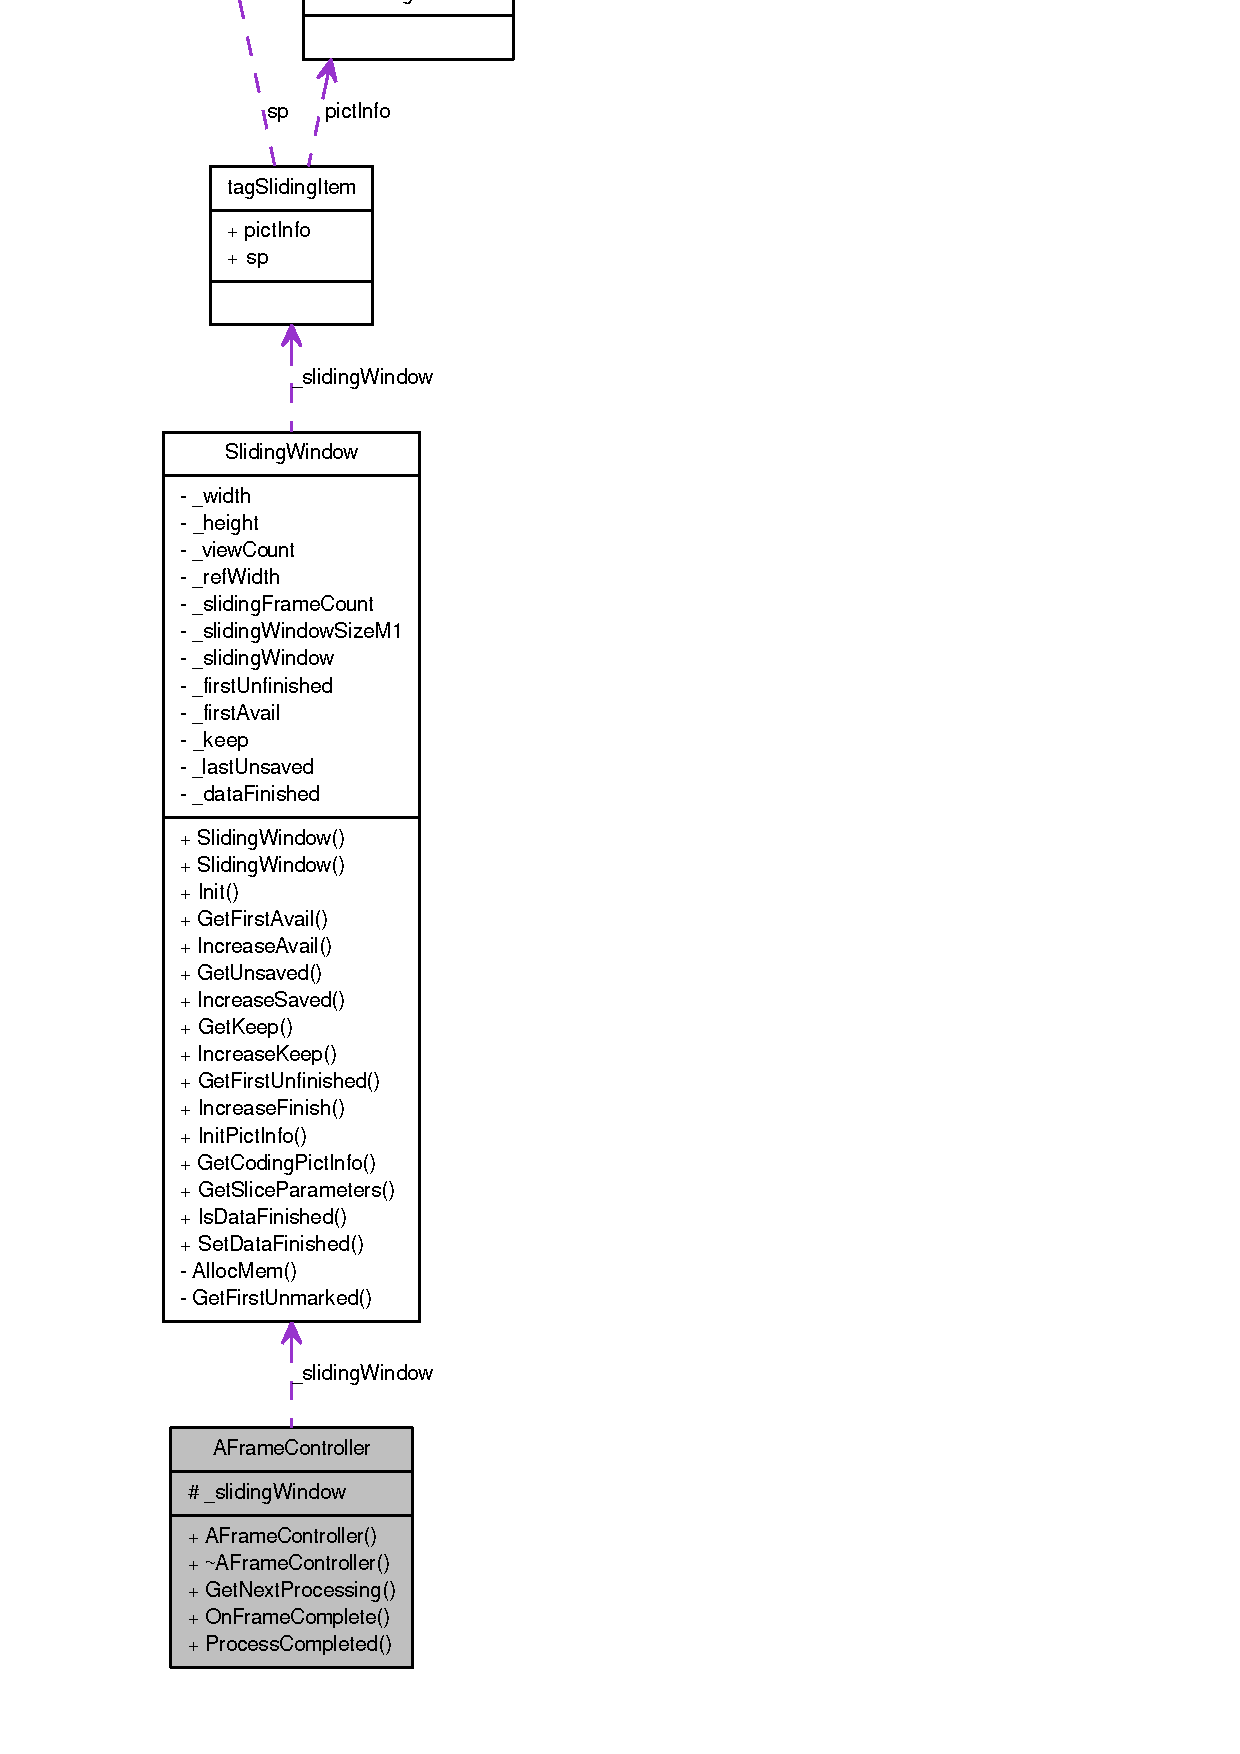
\includegraphics[height=400pt]{class_a_frame_controller__coll__graph}
\end{center}
\end{figure}
\subsection*{Public Member Functions}
\begin{DoxyCompactItemize}
\item 
\hyperlink{class_a_frame_controller_a448319ad03f91eebc5da7fdf8a43516c}{AFrameController} (\hyperlink{class_sliding_window}{SlidingWindow} $\ast$slidingWindow)
\item 
virtual \hyperlink{class_a_frame_controller_a71b793347efaa6e35b494ae728739ad0}{$\sim$AFrameController} ()
\item 
virtual \hyperlink{struct_coding_pict_info}{CodingPictInfo} $\ast$ \hyperlink{class_a_frame_controller_acc142fa10ce535ee171698af719c4d27}{GetNextProcessing} ()=0
\item 
virtual void \hyperlink{class_a_frame_controller_afd4834463eebfc33536fed009bfb966c}{OnFrameComplete} (\hyperlink{struct_coding_pict_info}{CodingPictInfo} $\ast$cpi)=0
\item 
virtual bool \hyperlink{class_a_frame_controller_a92ba4b7f8c0c84fff8be7203fae5221d}{ProcessCompleted} ()=0
\end{DoxyCompactItemize}
\subsection*{Protected Attributes}
\begin{DoxyCompactItemize}
\item 
\hyperlink{class_sliding_window}{SlidingWindow} $\ast$ \hyperlink{class_a_frame_controller_aca7790494d5c5d114171269ddaabd568}{\_\-slidingWindow}
\end{DoxyCompactItemize}


\subsection{Constructor \& Destructor Documentation}
\hypertarget{class_a_frame_controller_a448319ad03f91eebc5da7fdf8a43516c}{
\index{AFrameController@{AFrameController}!AFrameController@{AFrameController}}
\index{AFrameController@{AFrameController}!AFrameController@{AFrameController}}
\subsubsection[{AFrameController}]{\setlength{\rightskip}{0pt plus 5cm}AFrameController::AFrameController ({\bf SlidingWindow} $\ast$ {\em slidingWindow})\hspace{0.3cm}{\ttfamily  \mbox{[}inline\mbox{]}}}}
\label{class_a_frame_controller_a448319ad03f91eebc5da7fdf8a43516c}




\begin{footnotesize}\begin{alltt}
00029                                                        : \hyperlink{class_a_frame_controller_aca7790494d5c5d114171269ddaabd568}{_slidingWindow}(slidingWi
      ndow)
00030         \{
00031 
00032         \}
\end{alltt}\end{footnotesize}


\hypertarget{class_a_frame_controller_a71b793347efaa6e35b494ae728739ad0}{
\index{AFrameController@{AFrameController}!$\sim$AFrameController@{$\sim$AFrameController}}
\index{$\sim$AFrameController@{$\sim$AFrameController}!AFrameController@{AFrameController}}
\subsubsection[{$\sim$AFrameController}]{\setlength{\rightskip}{0pt plus 5cm}virtual AFrameController::$\sim$AFrameController ()\hspace{0.3cm}{\ttfamily  \mbox{[}inline, virtual\mbox{]}}}}
\label{class_a_frame_controller_a71b793347efaa6e35b494ae728739ad0}




\begin{footnotesize}\begin{alltt}
00034         \{
00035         \}
\end{alltt}\end{footnotesize}




\subsection{Member Function Documentation}
\hypertarget{class_a_frame_controller_acc142fa10ce535ee171698af719c4d27}{
\index{AFrameController@{AFrameController}!GetNextProcessing@{GetNextProcessing}}
\index{GetNextProcessing@{GetNextProcessing}!AFrameController@{AFrameController}}
\subsubsection[{GetNextProcessing}]{\setlength{\rightskip}{0pt plus 5cm}virtual {\bf CodingPictInfo}$\ast$ AFrameController::GetNextProcessing ()\hspace{0.3cm}{\ttfamily  \mbox{[}pure virtual\mbox{]}}}}
\label{class_a_frame_controller_acc142fa10ce535ee171698af719c4d27}


Implemented in \hyperlink{class_frame_controller___parallel_a51792b5fe70db6d99be59c110dbc3041}{FrameController\_\-Parallel}.



Here is the caller graph for this function:\nopagebreak
\begin{figure}[H]
\begin{center}
\leavevmode
\includegraphics[width=212pt]{class_a_frame_controller_acc142fa10ce535ee171698af719c4d27_icgraph}
\end{center}
\end{figure}


\hypertarget{class_a_frame_controller_afd4834463eebfc33536fed009bfb966c}{
\index{AFrameController@{AFrameController}!OnFrameComplete@{OnFrameComplete}}
\index{OnFrameComplete@{OnFrameComplete}!AFrameController@{AFrameController}}
\subsubsection[{OnFrameComplete}]{\setlength{\rightskip}{0pt plus 5cm}virtual void AFrameController::OnFrameComplete ({\bf CodingPictInfo} $\ast$ {\em cpi})\hspace{0.3cm}{\ttfamily  \mbox{[}pure virtual\mbox{]}}}}
\label{class_a_frame_controller_afd4834463eebfc33536fed009bfb966c}


Implemented in \hyperlink{class_frame_controller___parallel_a26429e70ddf3aa68cc2d28000a4935e1}{FrameController\_\-Parallel}.



Here is the caller graph for this function:\nopagebreak
\begin{figure}[H]
\begin{center}
\leavevmode
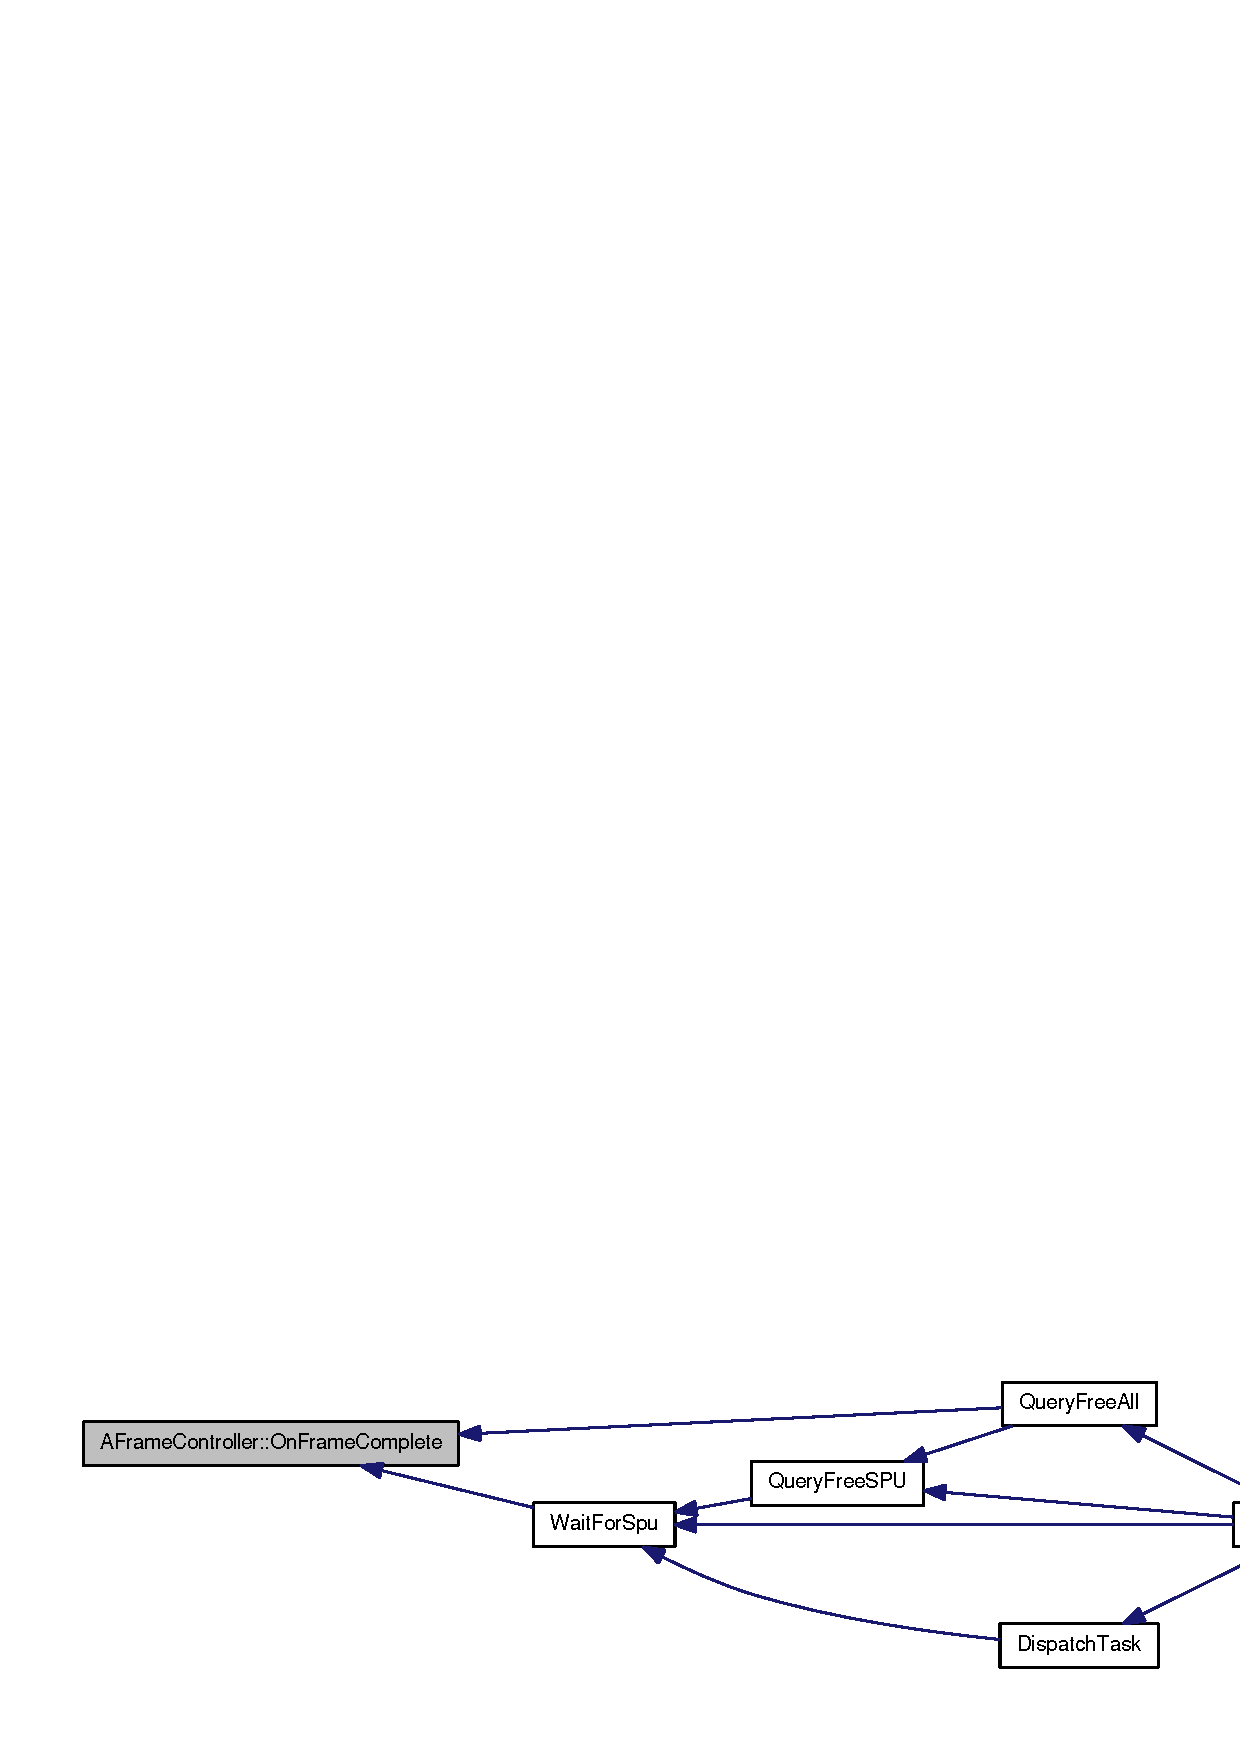
\includegraphics[width=378pt]{class_a_frame_controller_afd4834463eebfc33536fed009bfb966c_icgraph}
\end{center}
\end{figure}


\hypertarget{class_a_frame_controller_a92ba4b7f8c0c84fff8be7203fae5221d}{
\index{AFrameController@{AFrameController}!ProcessCompleted@{ProcessCompleted}}
\index{ProcessCompleted@{ProcessCompleted}!AFrameController@{AFrameController}}
\subsubsection[{ProcessCompleted}]{\setlength{\rightskip}{0pt plus 5cm}virtual bool AFrameController::ProcessCompleted ()\hspace{0.3cm}{\ttfamily  \mbox{[}pure virtual\mbox{]}}}}
\label{class_a_frame_controller_a92ba4b7f8c0c84fff8be7203fae5221d}


Implemented in \hyperlink{class_frame_controller___parallel_ac778eb523c6725a9e4da4e4239a88b2a}{FrameController\_\-Parallel}.



Here is the caller graph for this function:\nopagebreak
\begin{figure}[H]
\begin{center}
\leavevmode
\includegraphics[width=211pt]{class_a_frame_controller_a92ba4b7f8c0c84fff8be7203fae5221d_icgraph}
\end{center}
\end{figure}




\subsection{Member Data Documentation}
\hypertarget{class_a_frame_controller_aca7790494d5c5d114171269ddaabd568}{
\index{AFrameController@{AFrameController}!\_\-slidingWindow@{\_\-slidingWindow}}
\index{\_\-slidingWindow@{\_\-slidingWindow}!AFrameController@{AFrameController}}
\subsubsection[{\_\-slidingWindow}]{\setlength{\rightskip}{0pt plus 5cm}{\bf SlidingWindow}$\ast$ {\bf AFrameController::\_\-slidingWindow}\hspace{0.3cm}{\ttfamily  \mbox{[}protected\mbox{]}}}}
\label{class_a_frame_controller_aca7790494d5c5d114171269ddaabd568}


The documentation for this class was generated from the following file:\begin{DoxyCompactItemize}
\item 
MVCDecoder/Controller/\hyperlink{_a_frame_controller_8h}{AFrameController.h}\end{DoxyCompactItemize}

\hypertarget{class_array_list}{
\section{ArrayList$<$ T $>$ Class Template Reference}
\label{class_array_list}\index{ArrayList@{ArrayList}}
}


{\ttfamily \#include $<$ArrayList.h$>$}

\subsection*{Public Member Functions}
\begin{DoxyCompactItemize}
\item 
\hyperlink{class_array_list_a77ba51ae82bb2246563af5c4d64d438e}{ArrayList} ()
\item 
\hyperlink{class_array_list_aa4936cd0b9423eba7a9f38f3c62cfc7c}{ArrayList} (const \hyperlink{class_array_list}{ArrayList} \&right)
\item 
\hyperlink{class_array_list_a4af637822f64b61267b1e0ed4d4fca33}{$\sim$ArrayList} ()
\item 
\hyperlink{class_array_list}{ArrayList} \& \hyperlink{class_array_list_ae27782de18cb09f54fffba59f3f77d92}{operator=} (const \hyperlink{class_array_list}{ArrayList} \&right)
\item 
const T \& \hyperlink{class_array_list_a627f1cc60e0b9a85d869957a839bc064}{operator\mbox{[}$\,$\mbox{]}} (int index) const 
\item 
T \& \hyperlink{class_array_list_aaf3e10ff2125cc396e3c5d357bf94f1e}{operator\mbox{[}$\,$\mbox{]}} (int index)
\item 
int \hyperlink{class_array_list_aff9c6ac40886044e4653174950d23e74}{size} () const 
\item 
void \hyperlink{class_array_list_a7b5376678a9b5af0e0ed913fbe04b902}{push\_\-back} (const T \&value)
\item 
void \hyperlink{class_array_list_ad98cc674ef8dcc42f53b4836416a289c}{pop\_\-back} ()
\item 
void \hyperlink{class_array_list_a18695cf2c26e9c6ef585ec77afc19fc6}{erase} (int index)
\item 
void \hyperlink{class_array_list_addb12a5554260fa1f386160ce8534db0}{insert} (int index, const T \&value)
\item 
void \hyperlink{class_array_list_acb53d54675318c94332d0ec8b6819eb3}{clear} ()
\end{DoxyCompactItemize}
\subsubsection*{template$<$class T$>$ class ArrayList$<$ T $>$}



\subsection{Constructor \& Destructor Documentation}
\hypertarget{class_array_list_a77ba51ae82bb2246563af5c4d64d438e}{
\index{ArrayList@{ArrayList}!ArrayList@{ArrayList}}
\index{ArrayList@{ArrayList}!ArrayList@{ArrayList}}
\subsubsection[{ArrayList}]{\setlength{\rightskip}{0pt plus 5cm}template$<$class T$>$ {\bf ArrayList}$<$ T $>$::{\bf ArrayList} ()\hspace{0.3cm}{\ttfamily  \mbox{[}inline\mbox{]}}}}
\label{class_array_list_a77ba51ae82bb2246563af5c4d64d438e}




\begin{footnotesize}\begin{alltt}
00038                     : \_values(0), \_count(0), \_capacity(0)
00039         \{
00040         \}
\end{alltt}\end{footnotesize}


\hypertarget{class_array_list_aa4936cd0b9423eba7a9f38f3c62cfc7c}{
\index{ArrayList@{ArrayList}!ArrayList@{ArrayList}}
\index{ArrayList@{ArrayList}!ArrayList@{ArrayList}}
\subsubsection[{ArrayList}]{\setlength{\rightskip}{0pt plus 5cm}template$<$class T$>$ {\bf ArrayList}$<$ T $>$::{\bf ArrayList} (const {\bf ArrayList}$<$ T $>$ \& {\em right})\hspace{0.3cm}{\ttfamily  \mbox{[}inline\mbox{]}}}}
\label{class_array_list_aa4936cd0b9423eba7a9f38f3c62cfc7c}




\begin{footnotesize}\begin{alltt}
00042                                           : \_values(0), \_count(0), \_capacity(0)
00043         \{
00044                 *\textcolor{keyword}{this} = right;
00045         \}
\end{alltt}\end{footnotesize}


\hypertarget{class_array_list_a4af637822f64b61267b1e0ed4d4fca33}{
\index{ArrayList@{ArrayList}!$\sim$ArrayList@{$\sim$ArrayList}}
\index{$\sim$ArrayList@{$\sim$ArrayList}!ArrayList@{ArrayList}}
\subsubsection[{$\sim$ArrayList}]{\setlength{\rightskip}{0pt plus 5cm}template$<$class T$>$ {\bf ArrayList}$<$ T $>$::$\sim${\bf ArrayList} ()\hspace{0.3cm}{\ttfamily  \mbox{[}inline\mbox{]}}}}
\label{class_array_list_a4af637822f64b61267b1e0ed4d4fca33}




\begin{footnotesize}\begin{alltt}
00047                      \{
00048                 \textcolor{keyword}{delete}[] \_values;
00049         \}
\end{alltt}\end{footnotesize}




\subsection{Member Function Documentation}
\hypertarget{class_array_list_acb53d54675318c94332d0ec8b6819eb3}{
\index{ArrayList@{ArrayList}!clear@{clear}}
\index{clear@{clear}!ArrayList@{ArrayList}}
\subsubsection[{clear}]{\setlength{\rightskip}{0pt plus 5cm}template$<$class T$>$ void {\bf ArrayList}$<$ T $>$::clear ()\hspace{0.3cm}{\ttfamily  \mbox{[}inline\mbox{]}}}}
\label{class_array_list_acb53d54675318c94332d0ec8b6819eb3}




\begin{footnotesize}\begin{alltt}
00103         \{
00104                 \_count = 0;
00105         \}
\end{alltt}\end{footnotesize}




Here is the caller graph for this function:\nopagebreak
\begin{figure}[H]
\begin{center}
\leavevmode
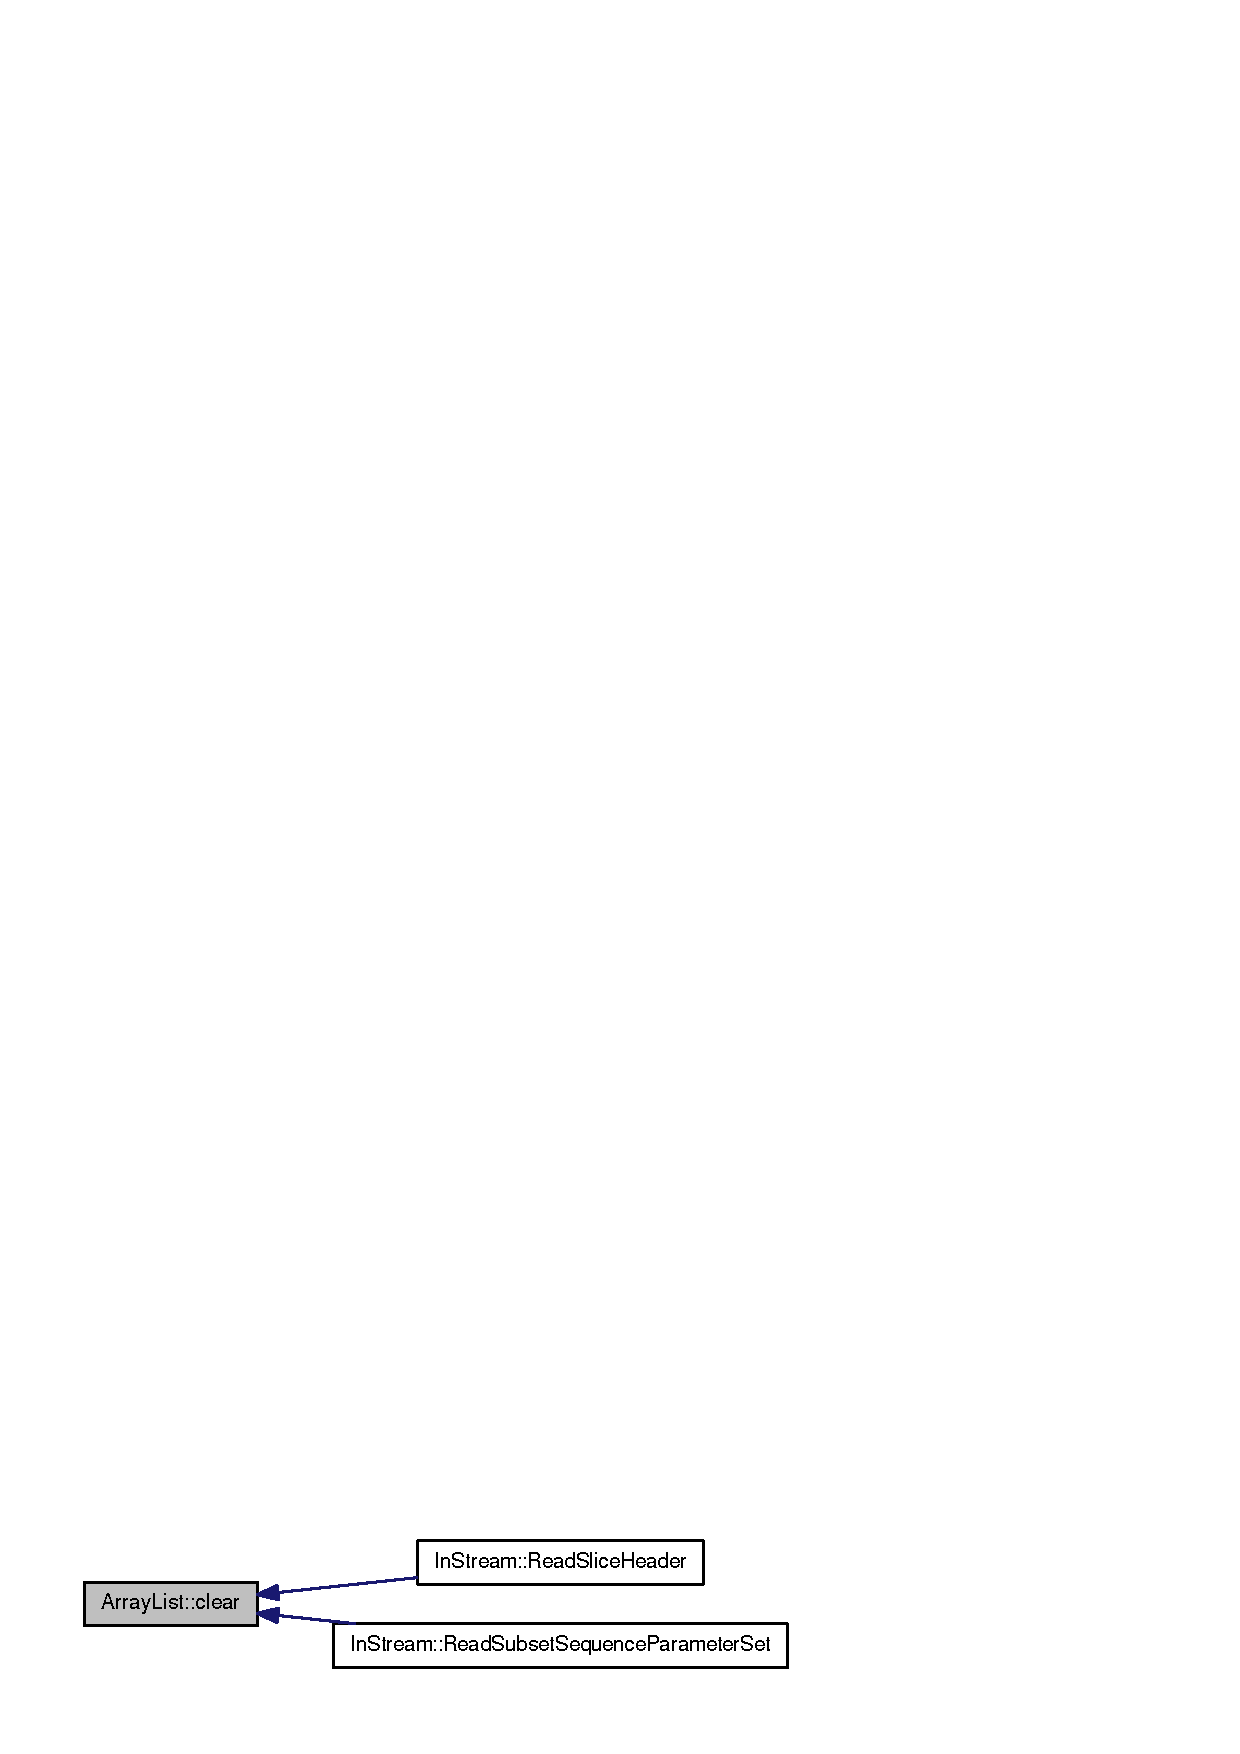
\includegraphics[width=191pt]{class_array_list_acb53d54675318c94332d0ec8b6819eb3_icgraph}
\end{center}
\end{figure}


\hypertarget{class_array_list_a18695cf2c26e9c6ef585ec77afc19fc6}{
\index{ArrayList@{ArrayList}!erase@{erase}}
\index{erase@{erase}!ArrayList@{ArrayList}}
\subsubsection[{erase}]{\setlength{\rightskip}{0pt plus 5cm}template$<$class T$>$ void {\bf ArrayList}$<$ T $>$::erase (int {\em index})\hspace{0.3cm}{\ttfamily  \mbox{[}inline\mbox{]}}}}
\label{class_array_list_a18695cf2c26e9c6ef585ec77afc19fc6}




\begin{footnotesize}\begin{alltt}
00087         \{
00088                 \textcolor{keywordflow}{for} (\textcolor{keywordtype}{int} i = index; i + 1 < \_count; ++i)
00089                         \_values[i] = \_values[i + 1];
00090                 --\_count;
00091         \}
\end{alltt}\end{footnotesize}




Here is the caller graph for this function:\nopagebreak
\begin{figure}[H]
\begin{center}
\leavevmode
\includegraphics[width=152pt]{class_array_list_a18695cf2c26e9c6ef585ec77afc19fc6_icgraph}
\end{center}
\end{figure}


\hypertarget{class_array_list_addb12a5554260fa1f386160ce8534db0}{
\index{ArrayList@{ArrayList}!insert@{insert}}
\index{insert@{insert}!ArrayList@{ArrayList}}
\subsubsection[{insert}]{\setlength{\rightskip}{0pt plus 5cm}template$<$class T$>$ void {\bf ArrayList}$<$ T $>$::insert (int {\em index}, \/  const T \& {\em value})\hspace{0.3cm}{\ttfamily  \mbox{[}inline\mbox{]}}}}
\label{class_array_list_addb12a5554260fa1f386160ce8534db0}




\begin{footnotesize}\begin{alltt}
00094         \{
00095                 RequireCapacity(\_count + 1);
00096                 \textcolor{keywordflow}{for} (\textcolor{keywordtype}{int} i = \_count; i > index; --i)
00097                         \_values[i] = \_values[i - 1];
00098                 \_values[index] = value;
00099                 ++\_count;
00100         \}
\end{alltt}\end{footnotesize}




Here is the caller graph for this function:\nopagebreak
\begin{figure}[H]
\begin{center}
\leavevmode
\includegraphics[width=152pt]{class_array_list_addb12a5554260fa1f386160ce8534db0_icgraph}
\end{center}
\end{figure}


\hypertarget{class_array_list_ae27782de18cb09f54fffba59f3f77d92}{
\index{ArrayList@{ArrayList}!operator=@{operator=}}
\index{operator=@{operator=}!ArrayList@{ArrayList}}
\subsubsection[{operator=}]{\setlength{\rightskip}{0pt plus 5cm}template$<$class T$>$ {\bf ArrayList}\& {\bf ArrayList}$<$ T $>$::operator= (const {\bf ArrayList}$<$ T $>$ \& {\em right})\hspace{0.3cm}{\ttfamily  \mbox{[}inline\mbox{]}}}}
\label{class_array_list_ae27782de18cb09f54fffba59f3f77d92}




\begin{footnotesize}\begin{alltt}
00052         \{
00053                 RequireCapacity(right.\_count);
00054                 \_count = right.\_count;
00055                 \textcolor{keywordflow}{for} (\textcolor{keywordtype}{int} i = 0; i < \_count; ++i)
00056                         \_values[i] = right.\_values[i];
00057                 \textcolor{keywordflow}{return} *\textcolor{keyword}{this};
00058         \}
\end{alltt}\end{footnotesize}


\hypertarget{class_array_list_aaf3e10ff2125cc396e3c5d357bf94f1e}{
\index{ArrayList@{ArrayList}!operator\mbox{[}\mbox{]}@{operator[]}}
\index{operator\mbox{[}\mbox{]}@{operator[]}!ArrayList@{ArrayList}}
\subsubsection[{operator[]}]{\setlength{\rightskip}{0pt plus 5cm}template$<$class T$>$ T\& {\bf ArrayList}$<$ T $>$::operator\mbox{[}$\,$\mbox{]} (int {\em index})\hspace{0.3cm}{\ttfamily  \mbox{[}inline\mbox{]}}}}
\label{class_array_list_aaf3e10ff2125cc396e3c5d357bf94f1e}




\begin{footnotesize}\begin{alltt}
00066         \{
00067                 \textcolor{keywordflow}{return} \_values[index];
00068         \}
\end{alltt}\end{footnotesize}


\hypertarget{class_array_list_a627f1cc60e0b9a85d869957a839bc064}{
\index{ArrayList@{ArrayList}!operator\mbox{[}\mbox{]}@{operator[]}}
\index{operator\mbox{[}\mbox{]}@{operator[]}!ArrayList@{ArrayList}}
\subsubsection[{operator[]}]{\setlength{\rightskip}{0pt plus 5cm}template$<$class T$>$ const T\& {\bf ArrayList}$<$ T $>$::operator\mbox{[}$\,$\mbox{]} (int {\em index}) const\hspace{0.3cm}{\ttfamily  \mbox{[}inline\mbox{]}}}}
\label{class_array_list_a627f1cc60e0b9a85d869957a839bc064}




\begin{footnotesize}\begin{alltt}
00061         \{
00062                 \textcolor{keywordflow}{return} \_values[index];
00063         \}
\end{alltt}\end{footnotesize}


\hypertarget{class_array_list_ad98cc674ef8dcc42f53b4836416a289c}{
\index{ArrayList@{ArrayList}!pop\_\-back@{pop\_\-back}}
\index{pop\_\-back@{pop\_\-back}!ArrayList@{ArrayList}}
\subsubsection[{pop\_\-back}]{\setlength{\rightskip}{0pt plus 5cm}template$<$class T$>$ void {\bf ArrayList}$<$ T $>$::pop\_\-back ()\hspace{0.3cm}{\ttfamily  \mbox{[}inline\mbox{]}}}}
\label{class_array_list_ad98cc674ef8dcc42f53b4836416a289c}




\begin{footnotesize}\begin{alltt}
00082         \{
00083                 --\_count;
00084         \}
\end{alltt}\end{footnotesize}




Here is the caller graph for this function:\nopagebreak
\begin{figure}[H]
\begin{center}
\leavevmode
\includegraphics[width=161pt]{class_array_list_ad98cc674ef8dcc42f53b4836416a289c_icgraph}
\end{center}
\end{figure}


\hypertarget{class_array_list_a7b5376678a9b5af0e0ed913fbe04b902}{
\index{ArrayList@{ArrayList}!push\_\-back@{push\_\-back}}
\index{push\_\-back@{push\_\-back}!ArrayList@{ArrayList}}
\subsubsection[{push\_\-back}]{\setlength{\rightskip}{0pt plus 5cm}template$<$class T$>$ void {\bf ArrayList}$<$ T $>$::push\_\-back (const T \& {\em value})\hspace{0.3cm}{\ttfamily  \mbox{[}inline\mbox{]}}}}
\label{class_array_list_a7b5376678a9b5af0e0ed913fbe04b902}




\begin{footnotesize}\begin{alltt}
00076         \{
00077                 RequireCapacity(\_count + 1);
00078                 \_values[\_count++] = value;
00079         \}
\end{alltt}\end{footnotesize}




Here is the caller graph for this function:\nopagebreak
\begin{figure}[H]
\begin{center}
\leavevmode
\includegraphics[width=204pt]{class_array_list_a7b5376678a9b5af0e0ed913fbe04b902_icgraph}
\end{center}
\end{figure}


\hypertarget{class_array_list_aff9c6ac40886044e4653174950d23e74}{
\index{ArrayList@{ArrayList}!size@{size}}
\index{size@{size}!ArrayList@{ArrayList}}
\subsubsection[{size}]{\setlength{\rightskip}{0pt plus 5cm}template$<$class T$>$ int {\bf ArrayList}$<$ T $>$::size () const\hspace{0.3cm}{\ttfamily  \mbox{[}inline\mbox{]}}}}
\label{class_array_list_aff9c6ac40886044e4653174950d23e74}




\begin{footnotesize}\begin{alltt}
00071         \{
00072                 \textcolor{keywordflow}{return} \_count;
00073         \}
\end{alltt}\end{footnotesize}




Here is the caller graph for this function:\nopagebreak
\begin{figure}[H]
\begin{center}
\leavevmode
\includegraphics[width=149pt]{class_array_list_aff9c6ac40886044e4653174950d23e74_icgraph}
\end{center}
\end{figure}




The documentation for this class was generated from the following file:\begin{DoxyCompactItemize}
\item 
MVCCommonLib/\hyperlink{_array_list_8h}{ArrayList.h}\end{DoxyCompactItemize}

\hypertarget{struct_bitstream}{
\section{Bitstream Struct Reference}
\label{struct_bitstream}\index{Bitstream@{Bitstream}}
}


{\ttfamily \#include $<$Bitstream.h$>$}

\subsection*{Public Attributes}
\begin{DoxyCompactItemize}
\item 
\hyperlink{_types_8h_a04909d1366bb244ff2482beb51635f37}{uint32\_\-t} \hyperlink{struct_bitstream_a2b3b7e703efb5f16a9b122862f6342ff}{bufa}
\item 
\hyperlink{_types_8h_a04909d1366bb244ff2482beb51635f37}{uint32\_\-t} \hyperlink{struct_bitstream_af88938159f6b589af03d736e9fe8119e}{bufb}
\item 
\hyperlink{_types_8h_a04909d1366bb244ff2482beb51635f37}{uint32\_\-t} \hyperlink{struct_bitstream_aa6e7d5fa7c3bcfaac4cda5c4b07f8aa1}{buf}
\item 
\hyperlink{_types_8h_a04909d1366bb244ff2482beb51635f37}{uint32\_\-t} \hyperlink{struct_bitstream_ac7479c4c4e57d10bbfdd90baf6e731a4}{pos}
\item 
\hyperlink{_types_8h_a04909d1366bb244ff2482beb51635f37}{uint32\_\-t} $\ast$ \hyperlink{struct_bitstream_addd740548c260796cf01e55597f749c6}{tail}
\item 
\hyperlink{_types_8h_a04909d1366bb244ff2482beb51635f37}{uint32\_\-t} $\ast$ \hyperlink{struct_bitstream_a4c2cb09a4fee7ed90d05f8b40914911e}{start}
\item 
\hyperlink{_types_8h_a04909d1366bb244ff2482beb51635f37}{uint32\_\-t} \hyperlink{struct_bitstream_a56ea589bea2ad26a4512ff556b055fd8}{length}
\item 
\hyperlink{_types_8h_a04909d1366bb244ff2482beb51635f37}{uint32\_\-t} \hyperlink{struct_bitstream_a3234ef24b4ec8a9d06731d4f2db67418}{initpos}
\end{DoxyCompactItemize}


\subsection{Member Data Documentation}
\hypertarget{struct_bitstream_aa6e7d5fa7c3bcfaac4cda5c4b07f8aa1}{
\index{Bitstream@{Bitstream}!buf@{buf}}
\index{buf@{buf}!Bitstream@{Bitstream}}
\subsubsection[{buf}]{\setlength{\rightskip}{0pt plus 5cm}{\bf uint32\_\-t} {\bf Bitstream::buf}}}
\label{struct_bitstream_aa6e7d5fa7c3bcfaac4cda5c4b07f8aa1}
\hypertarget{struct_bitstream_a2b3b7e703efb5f16a9b122862f6342ff}{
\index{Bitstream@{Bitstream}!bufa@{bufa}}
\index{bufa@{bufa}!Bitstream@{Bitstream}}
\subsubsection[{bufa}]{\setlength{\rightskip}{0pt plus 5cm}{\bf uint32\_\-t} {\bf Bitstream::bufa}}}
\label{struct_bitstream_a2b3b7e703efb5f16a9b122862f6342ff}
\hypertarget{struct_bitstream_af88938159f6b589af03d736e9fe8119e}{
\index{Bitstream@{Bitstream}!bufb@{bufb}}
\index{bufb@{bufb}!Bitstream@{Bitstream}}
\subsubsection[{bufb}]{\setlength{\rightskip}{0pt plus 5cm}{\bf uint32\_\-t} {\bf Bitstream::bufb}}}
\label{struct_bitstream_af88938159f6b589af03d736e9fe8119e}
\hypertarget{struct_bitstream_a3234ef24b4ec8a9d06731d4f2db67418}{
\index{Bitstream@{Bitstream}!initpos@{initpos}}
\index{initpos@{initpos}!Bitstream@{Bitstream}}
\subsubsection[{initpos}]{\setlength{\rightskip}{0pt plus 5cm}{\bf uint32\_\-t} {\bf Bitstream::initpos}}}
\label{struct_bitstream_a3234ef24b4ec8a9d06731d4f2db67418}
\hypertarget{struct_bitstream_a56ea589bea2ad26a4512ff556b055fd8}{
\index{Bitstream@{Bitstream}!length@{length}}
\index{length@{length}!Bitstream@{Bitstream}}
\subsubsection[{length}]{\setlength{\rightskip}{0pt plus 5cm}{\bf uint32\_\-t} {\bf Bitstream::length}}}
\label{struct_bitstream_a56ea589bea2ad26a4512ff556b055fd8}
\hypertarget{struct_bitstream_ac7479c4c4e57d10bbfdd90baf6e731a4}{
\index{Bitstream@{Bitstream}!pos@{pos}}
\index{pos@{pos}!Bitstream@{Bitstream}}
\subsubsection[{pos}]{\setlength{\rightskip}{0pt plus 5cm}{\bf uint32\_\-t} {\bf Bitstream::pos}}}
\label{struct_bitstream_ac7479c4c4e57d10bbfdd90baf6e731a4}
\hypertarget{struct_bitstream_a4c2cb09a4fee7ed90d05f8b40914911e}{
\index{Bitstream@{Bitstream}!start@{start}}
\index{start@{start}!Bitstream@{Bitstream}}
\subsubsection[{start}]{\setlength{\rightskip}{0pt plus 5cm}{\bf uint32\_\-t}$\ast$ {\bf Bitstream::start}}}
\label{struct_bitstream_a4c2cb09a4fee7ed90d05f8b40914911e}
\hypertarget{struct_bitstream_addd740548c260796cf01e55597f749c6}{
\index{Bitstream@{Bitstream}!tail@{tail}}
\index{tail@{tail}!Bitstream@{Bitstream}}
\subsubsection[{tail}]{\setlength{\rightskip}{0pt plus 5cm}{\bf uint32\_\-t}$\ast$ {\bf Bitstream::tail}}}
\label{struct_bitstream_addd740548c260796cf01e55597f749c6}


The documentation for this struct was generated from the following file:\begin{DoxyCompactItemize}
\item 
MVCCommonLib/Codec/\hyperlink{_bitstream_8h}{Bitstream.h}\end{DoxyCompactItemize}

\include{class_bitstream_data}
\hypertarget{class_block_debug}{
\section{BlockDebug Class Reference}
\label{class_block_debug}\index{BlockDebug@{BlockDebug}}
}


{\ttfamily \#include $<$Debug.h$>$}

\subsection*{Public Member Functions}
\begin{DoxyCompactItemize}
\item 
\hyperlink{class_block_debug_ad0b4c92c068d6a2c8c89df860df29b02}{BlockDebug} (const char $\ast$filename, int linenumber, int level)
\item 
\hyperlink{class_block_debug_ab104ecf455577f36f9f5ef176d53d8ae}{BlockDebug} (const char $\ast$filename, int linenumber, const char $\ast$info, int level)
\item 
\hyperlink{class_block_debug_a82a6d59776c3191a56b532ec23f6174e}{$\sim$BlockDebug} ()
\end{DoxyCompactItemize}


\subsection{Constructor \& Destructor Documentation}
\hypertarget{class_block_debug_ad0b4c92c068d6a2c8c89df860df29b02}{
\index{BlockDebug@{BlockDebug}!BlockDebug@{BlockDebug}}
\index{BlockDebug@{BlockDebug}!BlockDebug@{BlockDebug}}
\subsubsection[{BlockDebug}]{\setlength{\rightskip}{0pt plus 5cm}BlockDebug::BlockDebug (const char $\ast$ {\em filename}, \/  int {\em linenumber}, \/  int {\em level})\hspace{0.3cm}{\ttfamily  \mbox{[}inline\mbox{]}}}}
\label{class_block_debug_ad0b4c92c068d6a2c8c89df860df29b02}




\begin{footnotesize}\begin{alltt}
00075         \{
00076                 setinfo(filename, linenumber, \textcolor{stringliteral}{""}, level);
00077         \}
\end{alltt}\end{footnotesize}


\hypertarget{class_block_debug_ab104ecf455577f36f9f5ef176d53d8ae}{
\index{BlockDebug@{BlockDebug}!BlockDebug@{BlockDebug}}
\index{BlockDebug@{BlockDebug}!BlockDebug@{BlockDebug}}
\subsubsection[{BlockDebug}]{\setlength{\rightskip}{0pt plus 5cm}BlockDebug::BlockDebug (const char $\ast$ {\em filename}, \/  int {\em linenumber}, \/  const char $\ast$ {\em info}, \/  int {\em level})\hspace{0.3cm}{\ttfamily  \mbox{[}inline\mbox{]}}}}
\label{class_block_debug_ab104ecf455577f36f9f5ef176d53d8ae}




\begin{footnotesize}\begin{alltt}
00079         \{
00080                 setinfo(filename, linenumber, info, level);
00081         \}
\end{alltt}\end{footnotesize}


\hypertarget{class_block_debug_a82a6d59776c3191a56b532ec23f6174e}{
\index{BlockDebug@{BlockDebug}!$\sim$BlockDebug@{$\sim$BlockDebug}}
\index{$\sim$BlockDebug@{$\sim$BlockDebug}!BlockDebug@{BlockDebug}}
\subsubsection[{$\sim$BlockDebug}]{\setlength{\rightskip}{0pt plus 5cm}BlockDebug::$\sim$BlockDebug ()\hspace{0.3cm}{\ttfamily  \mbox{[}inline\mbox{]}}}}
\label{class_block_debug_a82a6d59776c3191a56b532ec23f6174e}




\begin{footnotesize}\begin{alltt}
00083         \{
00084                 \textcolor{keywordflow}{if} (lev >= \hyperlink{_debug_8h_a77b6b5782a3099e95b552c23366ace9b}{CURLEVEL})
00085                 \{
00086                         --\hyperlink{class_current_heap_a810bf94894ae33cb375e353219e6a209}{CurrentHeap::curHeap};
00087                         \hyperlink{_debug_8cpp_a5c2d38f133d73274898b1dd5844a1880}{printHeaps}();
00088                         printf(\textcolor{stringliteral}{"Leave Block %s(%d): %s\(\backslash\)n"}, filename, linenumber, 
      info);
00089                 \}
00090                 \textcolor{keyword}{delete}[] filename;
00091                 \textcolor{keyword}{delete}[] info;
00092         \}
\end{alltt}\end{footnotesize}




Here is the call graph for this function:\nopagebreak
\begin{figure}[H]
\begin{center}
\leavevmode
\includegraphics[width=139pt]{class_block_debug_a82a6d59776c3191a56b532ec23f6174e_cgraph}
\end{center}
\end{figure}




The documentation for this class was generated from the following file:\begin{DoxyCompactItemize}
\item 
MVCCommonLib/\hyperlink{_debug_8h}{Debug.h}\end{DoxyCompactItemize}

\hypertarget{class_codec_info}{
\section{CodecInfo Class Reference}
\label{class_codec_info}\index{CodecInfo@{CodecInfo}}
}


{\ttfamily \#include $<$CodecInfo.h$>$}



Collaboration diagram for CodecInfo:\nopagebreak
\begin{figure}[H]
\begin{center}
\leavevmode
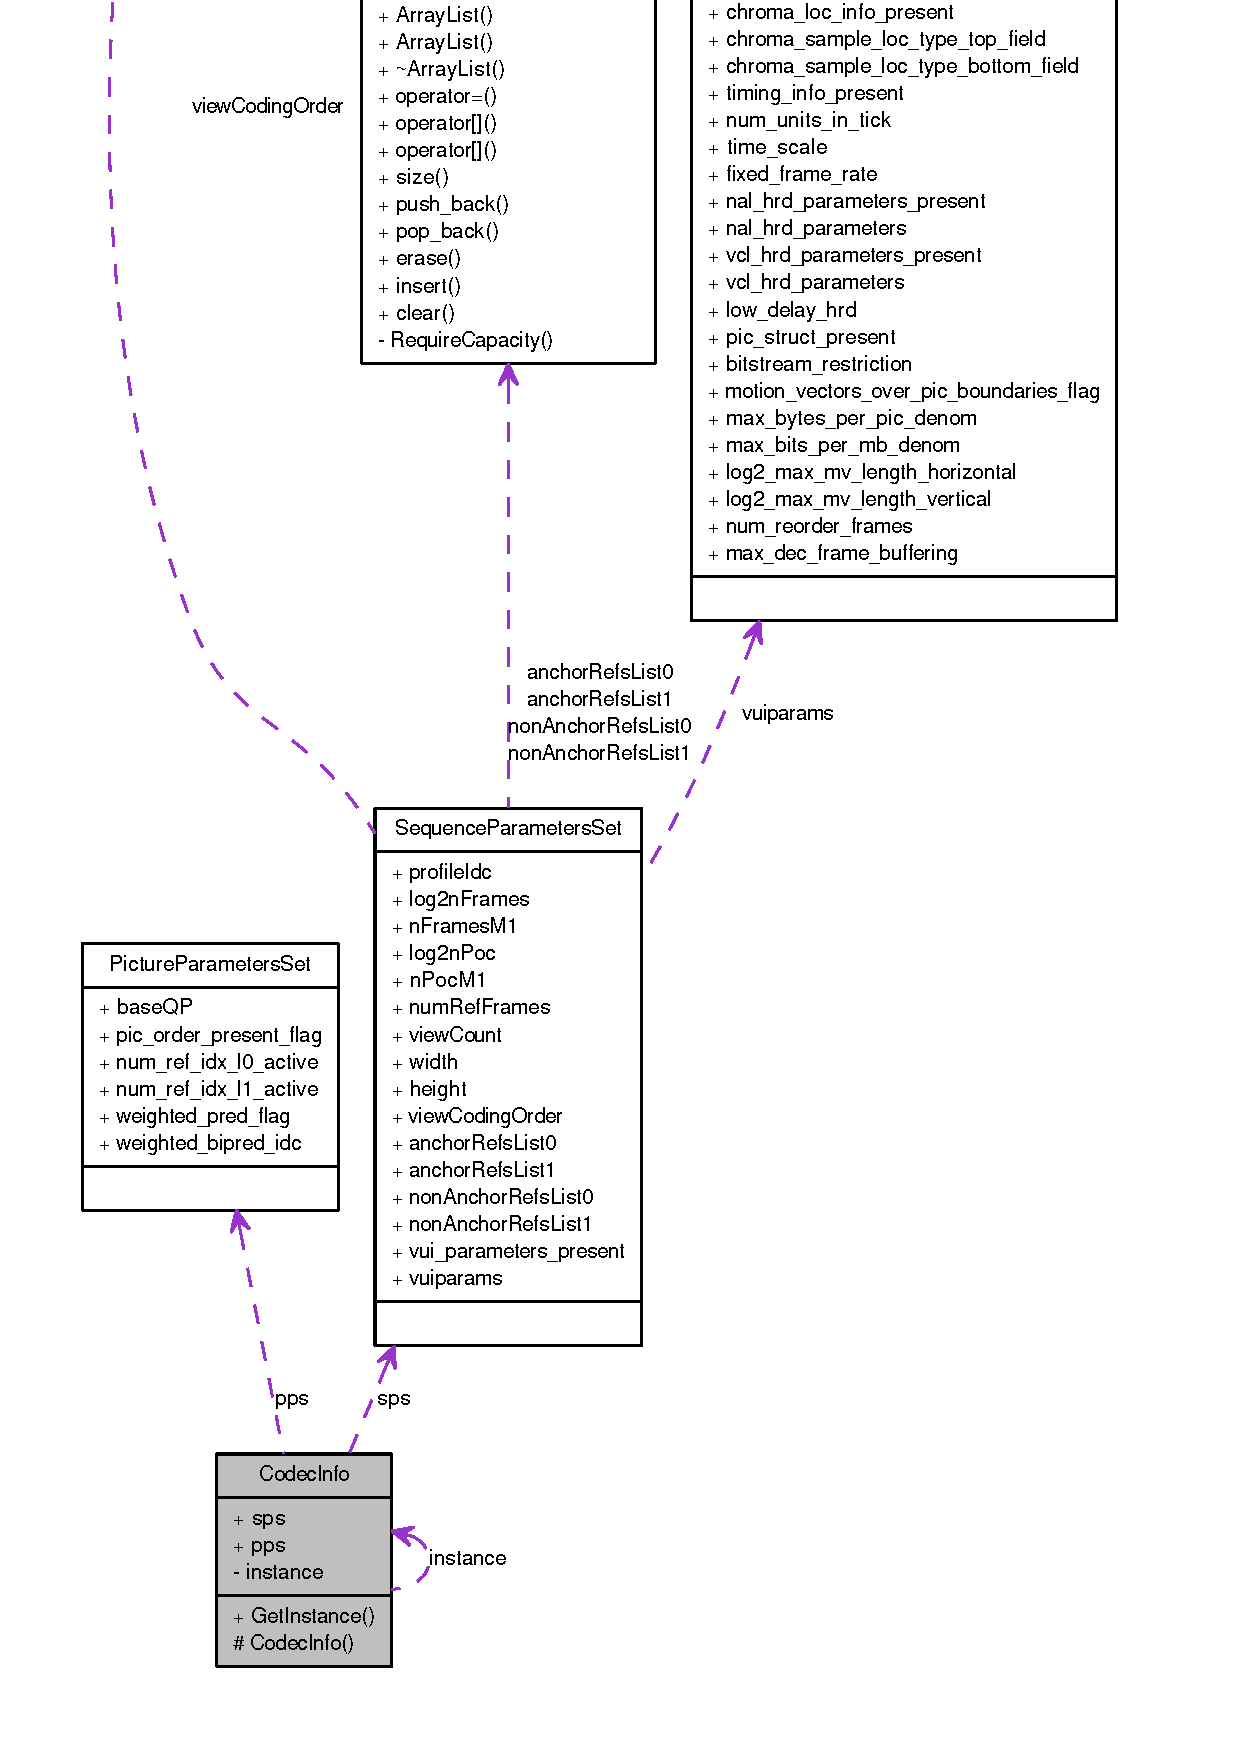
\includegraphics[width=400pt]{class_codec_info__coll__graph}
\end{center}
\end{figure}
\subsection*{Static Public Member Functions}
\begin{DoxyCompactItemize}
\item 
static \hyperlink{class_codec_info}{CodecInfo} \& \hyperlink{class_codec_info_ad439fd8062a03d868dfe9c9b615b747e}{GetInstance} ()
\end{DoxyCompactItemize}
\subsection*{Public Attributes}
\begin{DoxyCompactItemize}
\item 
\hyperlink{struct_sequence_parameters_set}{SequenceParametersSet} \hyperlink{class_codec_info_aee785011cec77ff3c0c646b498fe1e7d}{sps}
\item 
\hyperlink{struct_picture_parameters_set}{PictureParametersSet} \hyperlink{class_codec_info_abaa8d84a7d4045129ee64d91eaac4481}{pps}
\end{DoxyCompactItemize}
\subsection*{Protected Member Functions}
\begin{DoxyCompactItemize}
\item 
\hyperlink{class_codec_info_ab2ecf673aaa2480fafb0b3d22896e4b6}{CodecInfo} ()
\end{DoxyCompactItemize}


\subsection{Constructor \& Destructor Documentation}
\hypertarget{class_codec_info_ab2ecf673aaa2480fafb0b3d22896e4b6}{
\index{CodecInfo@{CodecInfo}!CodecInfo@{CodecInfo}}
\index{CodecInfo@{CodecInfo}!CodecInfo@{CodecInfo}}
\subsubsection[{CodecInfo}]{\setlength{\rightskip}{0pt plus 5cm}CodecInfo::CodecInfo ()\hspace{0.3cm}{\ttfamily  \mbox{[}inline, protected\mbox{]}}}}
\label{class_codec_info_ab2ecf673aaa2480fafb0b3d22896e4b6}




\begin{footnotesize}\begin{alltt}
00025                     \{
00026                 memset(&\hyperlink{class_codec_info_aee785011cec77ff3c0c646b498fe1e7d}{sps}, 0, \textcolor{keyword}{sizeof}(\hyperlink{class_codec_info_aee785011cec77ff3c0c646b498fe1e7d}{sps}));
00027                 memset(&\hyperlink{class_codec_info_abaa8d84a7d4045129ee64d91eaac4481}{pps}, 0, \textcolor{keyword}{sizeof}(\hyperlink{class_codec_info_abaa8d84a7d4045129ee64d91eaac4481}{pps}));
00028         \}
\end{alltt}\end{footnotesize}




Here is the caller graph for this function:\nopagebreak
\begin{figure}[H]
\begin{center}
\leavevmode
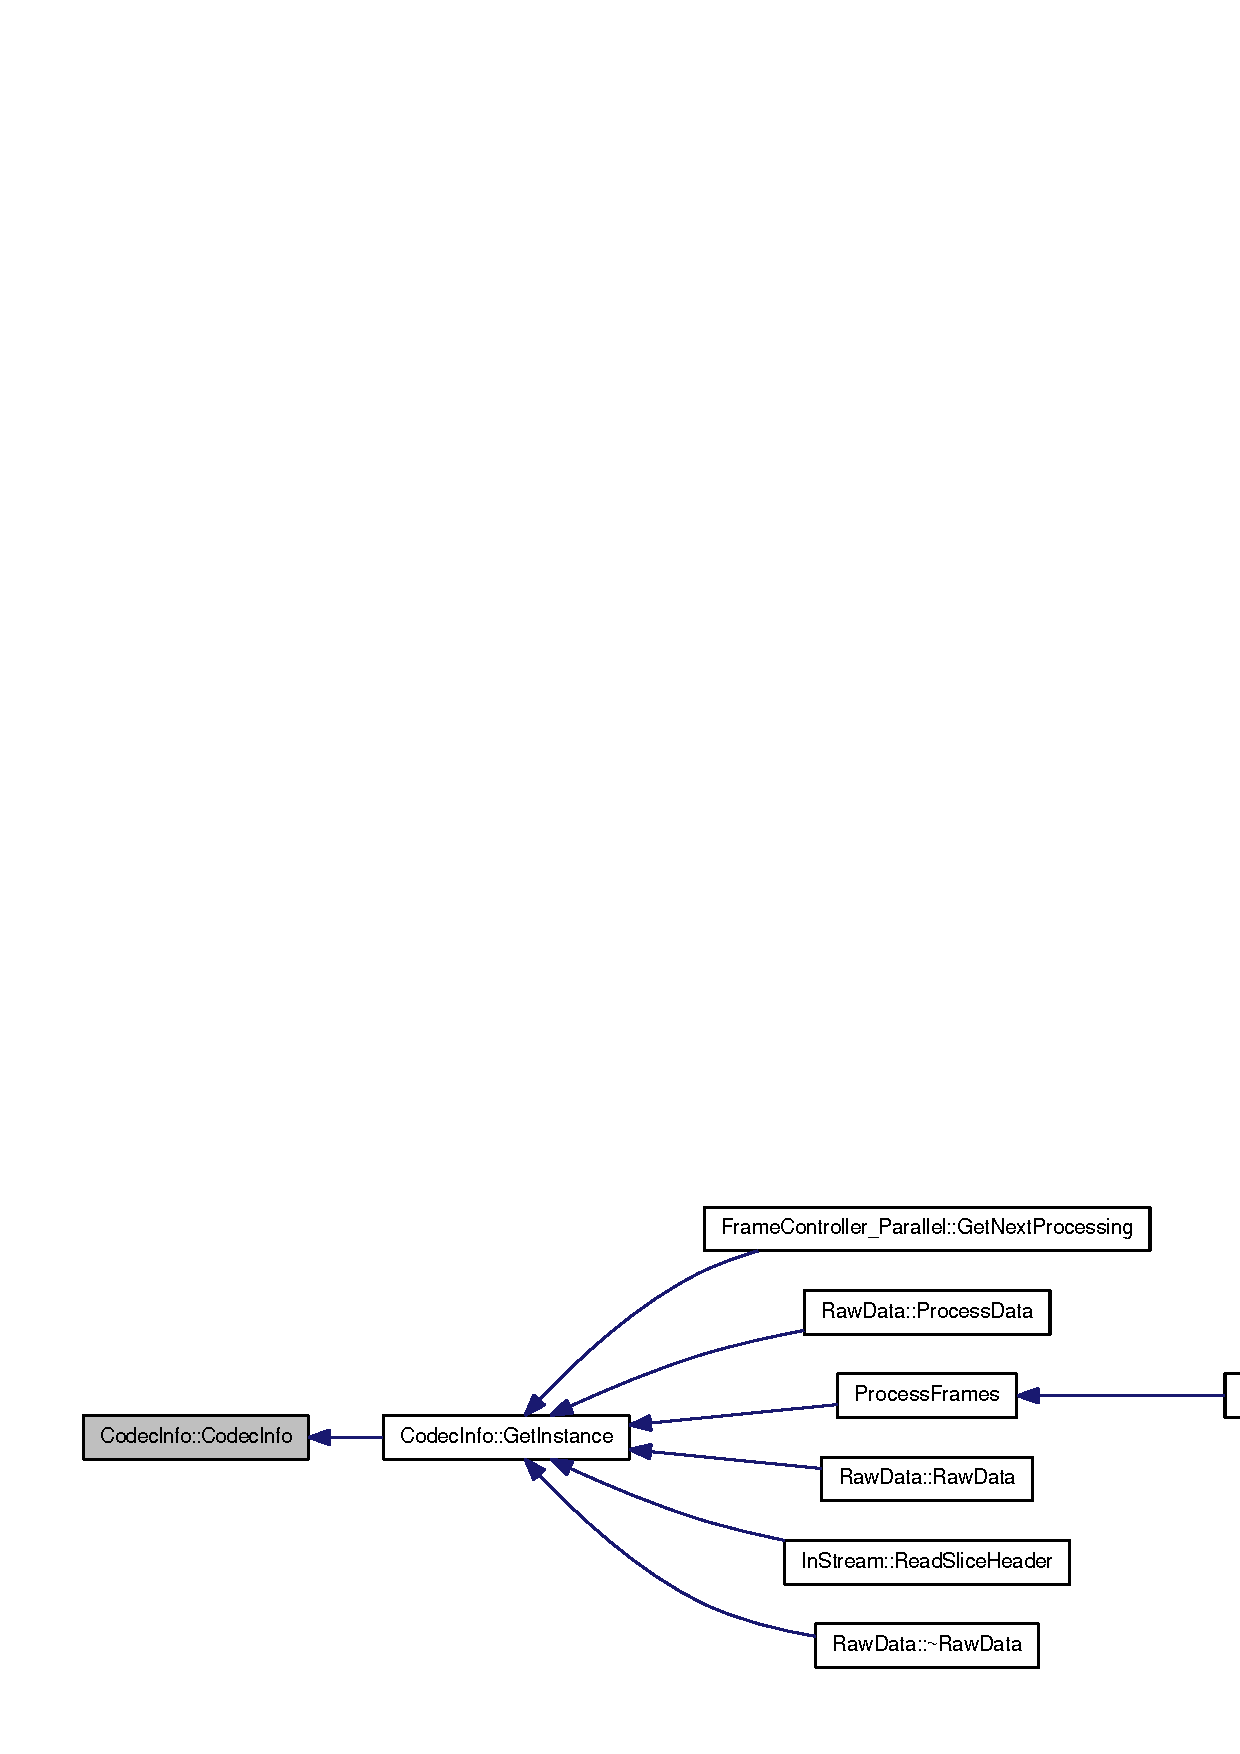
\includegraphics[width=315pt]{class_codec_info_ab2ecf673aaa2480fafb0b3d22896e4b6_icgraph}
\end{center}
\end{figure}




\subsection{Member Function Documentation}
\hypertarget{class_codec_info_ad439fd8062a03d868dfe9c9b615b747e}{
\index{CodecInfo@{CodecInfo}!GetInstance@{GetInstance}}
\index{GetInstance@{GetInstance}!CodecInfo@{CodecInfo}}
\subsubsection[{GetInstance}]{\setlength{\rightskip}{0pt plus 5cm}static {\bf CodecInfo}\& CodecInfo::GetInstance ()\hspace{0.3cm}{\ttfamily  \mbox{[}inline, static\mbox{]}}}}
\label{class_codec_info_ad439fd8062a03d868dfe9c9b615b747e}




\begin{footnotesize}\begin{alltt}
00031         \{
00032                 \textcolor{keywordflow}{if} (!instance)
00033                         instance = \textcolor{keyword}{new} \hyperlink{class_codec_info_ab2ecf673aaa2480fafb0b3d22896e4b6}{CodecInfo}();
00034                 \textcolor{keywordflow}{return} *instance;
00035         \}
\end{alltt}\end{footnotesize}




Here is the call graph for this function:\nopagebreak
\begin{figure}[H]
\begin{center}
\leavevmode
\includegraphics[width=153pt]{class_codec_info_ad439fd8062a03d868dfe9c9b615b747e_cgraph}
\end{center}
\end{figure}




Here is the caller graph for this function:\nopagebreak
\begin{figure}[H]
\begin{center}
\leavevmode
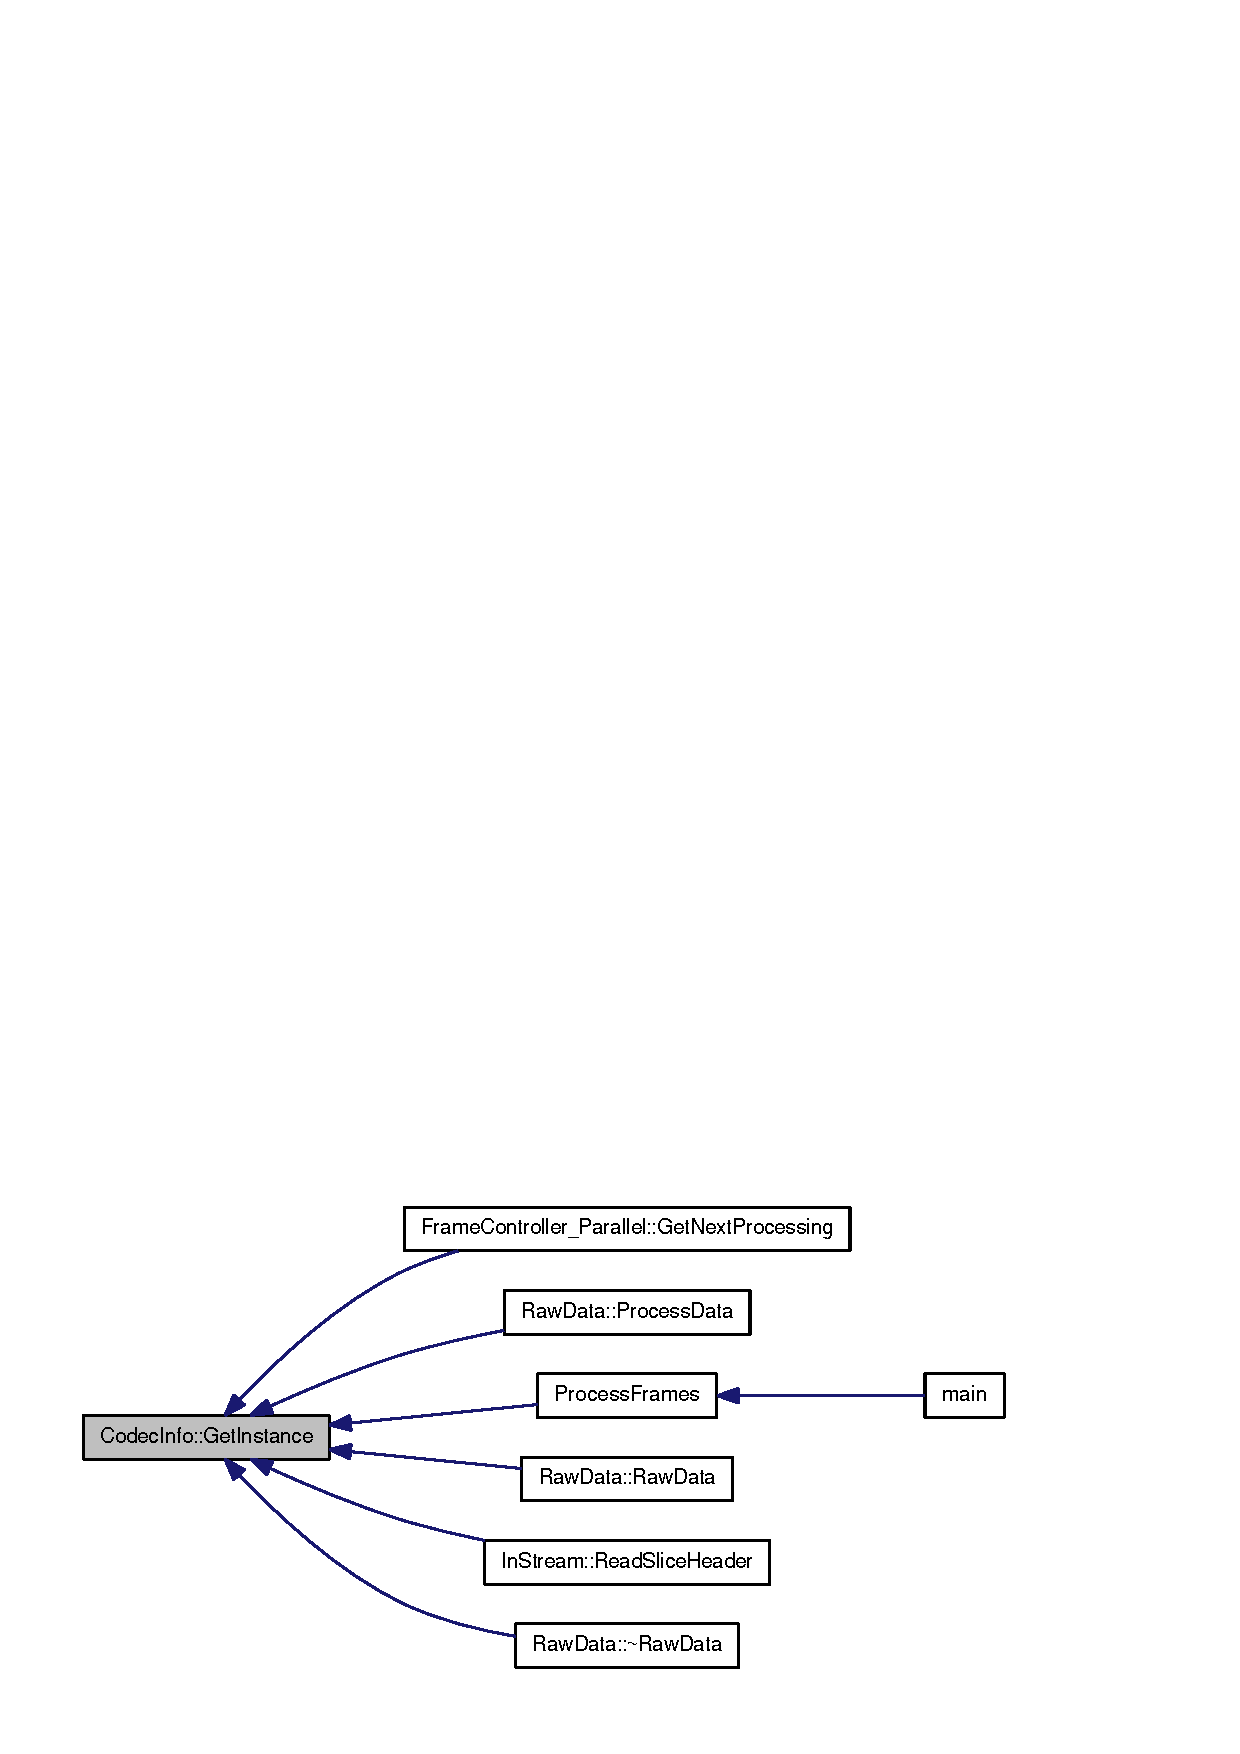
\includegraphics[width=243pt]{class_codec_info_ad439fd8062a03d868dfe9c9b615b747e_icgraph}
\end{center}
\end{figure}




\subsection{Member Data Documentation}
\hypertarget{class_codec_info_abaa8d84a7d4045129ee64d91eaac4481}{
\index{CodecInfo@{CodecInfo}!pps@{pps}}
\index{pps@{pps}!CodecInfo@{CodecInfo}}
\subsubsection[{pps}]{\setlength{\rightskip}{0pt plus 5cm}{\bf PictureParametersSet} {\bf CodecInfo::pps}}}
\label{class_codec_info_abaa8d84a7d4045129ee64d91eaac4481}
\hypertarget{class_codec_info_aee785011cec77ff3c0c646b498fe1e7d}{
\index{CodecInfo@{CodecInfo}!sps@{sps}}
\index{sps@{sps}!CodecInfo@{CodecInfo}}
\subsubsection[{sps}]{\setlength{\rightskip}{0pt plus 5cm}{\bf SequenceParametersSet} {\bf CodecInfo::sps}}}
\label{class_codec_info_aee785011cec77ff3c0c646b498fe1e7d}


The documentation for this class was generated from the following files:\begin{DoxyCompactItemize}
\item 
MVCDecoder/\hyperlink{_codec_info_8h}{CodecInfo.h}\item 
MVCDecoder/\hyperlink{_codec_info_8cpp}{CodecInfo.cpp}\end{DoxyCompactItemize}

\hypertarget{struct_coding_pict_info}{
\section{CodingPictInfo Struct Reference}
\label{struct_coding_pict_info}\index{CodingPictInfo@{CodingPictInfo}}
}


{\ttfamily \#include $<$PictureInfo.h$>$}

\subsection*{Public Attributes}
\begin{DoxyCompactItemize}
\item 
int \hyperlink{struct_coding_pict_info_a6bfb22b57d0d223546150c71e125fb39}{PictType}
\item 
int \hyperlink{struct_coding_pict_info_afeeb373571d44e64d473524e6127f3f7}{Size\_\-Width}
\item 
int \hyperlink{struct_coding_pict_info_aa6352dc53234c55d1a0c252c5b8d6141}{Size\_\-Height}
\item 
int \hyperlink{struct_coding_pict_info_ad85dae4751165ea3cbb8f7b8c6e61dc3}{timeId}
\item 
int \hyperlink{struct_coding_pict_info_a987595091bfba91b3166b04bca988697}{viewId}
\item 
int \hyperlink{struct_coding_pict_info_a6e808cdf552c3a18da4b75f4d0c35c28}{baseQP}
\item 
\hyperlink{_types_8h_a363e4d606232036a6b89060813c45489}{uint8\_\-t} $\ast$ \hyperlink{struct_coding_pict_info_a62aee8cc8c9cac725d4f44a19ddc8c2b}{lumaStart}
\item 
\hyperlink{_types_8h_a363e4d606232036a6b89060813c45489}{uint8\_\-t} $\ast$ \hyperlink{struct_coding_pict_info_a103a3180ba57db0bd984a53f0668b70b}{chromaUStart}
\item 
\hyperlink{_types_8h_a363e4d606232036a6b89060813c45489}{uint8\_\-t} $\ast$ \hyperlink{struct_coding_pict_info_a7be3395b2a1e7f4b384421c2490dcfdc}{chromaVStart}
\item 
int \hyperlink{struct_coding_pict_info_ab48541faa825385baeca833ffe98b3d4}{Ref\_\-Count} \mbox{[}2\mbox{]}
\item 
unsigned int \hyperlink{struct_coding_pict_info_a37079a7e9c26b338a6978063f471a82f}{Ref\_\-Id} \mbox{[}2\mbox{]}\mbox{[}4\mbox{]}\mbox{[}2\mbox{]}
\item 
\hyperlink{_types_8h_a363e4d606232036a6b89060813c45489}{uint8\_\-t} $\ast$ \hyperlink{struct_coding_pict_info_a8c8c3eeff0744de167b9ea6c5a7938a0}{ref\_\-lumaStart} \mbox{[}2\mbox{]}\mbox{[}4\mbox{]}
\item 
\hyperlink{_types_8h_a363e4d606232036a6b89060813c45489}{uint8\_\-t} $\ast$ \hyperlink{struct_coding_pict_info_a48b49b89c36f39af860936fbf3a3c991}{ref\_\-chromaUStart} \mbox{[}2\mbox{]}\mbox{[}4\mbox{]}
\item 
\hyperlink{_types_8h_a363e4d606232036a6b89060813c45489}{uint8\_\-t} $\ast$ \hyperlink{struct_coding_pict_info_a5c703063430f731196d3acea2926d5bd}{ref\_\-chromaVStart} \mbox{[}2\mbox{]}\mbox{[}4\mbox{]}
\item 
\hyperlink{_types_8h_a363e4d606232036a6b89060813c45489}{uint8\_\-t} $\ast$ \hyperlink{struct_coding_pict_info_a1c02c2f7c7a4a9fb4ed10e422d64bd32}{ref\_\-refVec} \mbox{[}2\mbox{]}\mbox{[}4\mbox{]}
\item 
\hyperlink{_types_8h_a363e4d606232036a6b89060813c45489}{uint8\_\-t} $\ast$ \hyperlink{struct_coding_pict_info_aa49520dd613a44185d6a41af8992d66c}{refVec}
\item 
\hyperlink{_types_8h_a363e4d606232036a6b89060813c45489}{uint8\_\-t} $\ast$ \hyperlink{struct_coding_pict_info_af53de7a35b8796df845ddee01d70fc5b}{resultStream}
\item 
\hyperlink{_types_8h_a115ba3a1b24a8702355c5dbd61ce01e0}{int32\_\-t} $\ast$ \hyperlink{struct_coding_pict_info_a37155b7c53db0a4a94d314bdc3c95104}{resultSize}
\item 
\hyperlink{_types_8h_a115ba3a1b24a8702355c5dbd61ce01e0}{int32\_\-t} \hyperlink{struct_coding_pict_info_a589da1ebbfa6493b63005412ce79dac6}{streamStart}
\item 
\hyperlink{_types_8h_a115ba3a1b24a8702355c5dbd61ce01e0}{int32\_\-t} \hyperlink{struct_coding_pict_info_a41498e5ba764405481005e6569d7f728}{pictStatus}
\item 
\hyperlink{_types_8h_a115ba3a1b24a8702355c5dbd61ce01e0}{int32\_\-t} \hyperlink{struct_coding_pict_info_ac290120f5d65f0497efa17928da82922}{log2nFrames}
\item 
\hyperlink{_types_8h_a115ba3a1b24a8702355c5dbd61ce01e0}{int32\_\-t} \hyperlink{struct_coding_pict_info_ab254953ed2b4e1de64f05eadbc825646}{MP}
\item 
int \hyperlink{struct_coding_pict_info_ad470102c0479d9d874fa68691a650581}{Padding} \mbox{[}1\mbox{]}
\end{DoxyCompactItemize}


\subsection{Member Data Documentation}
\hypertarget{struct_coding_pict_info_a6e808cdf552c3a18da4b75f4d0c35c28}{
\index{CodingPictInfo@{CodingPictInfo}!baseQP@{baseQP}}
\index{baseQP@{baseQP}!CodingPictInfo@{CodingPictInfo}}
\subsubsection[{baseQP}]{\setlength{\rightskip}{0pt plus 5cm}int {\bf CodingPictInfo::baseQP}}}
\label{struct_coding_pict_info_a6e808cdf552c3a18da4b75f4d0c35c28}
\hypertarget{struct_coding_pict_info_a103a3180ba57db0bd984a53f0668b70b}{
\index{CodingPictInfo@{CodingPictInfo}!chromaUStart@{chromaUStart}}
\index{chromaUStart@{chromaUStart}!CodingPictInfo@{CodingPictInfo}}
\subsubsection[{chromaUStart}]{\setlength{\rightskip}{0pt plus 5cm}{\bf uint8\_\-t}$\ast$ {\bf CodingPictInfo::chromaUStart}}}
\label{struct_coding_pict_info_a103a3180ba57db0bd984a53f0668b70b}
\hypertarget{struct_coding_pict_info_a7be3395b2a1e7f4b384421c2490dcfdc}{
\index{CodingPictInfo@{CodingPictInfo}!chromaVStart@{chromaVStart}}
\index{chromaVStart@{chromaVStart}!CodingPictInfo@{CodingPictInfo}}
\subsubsection[{chromaVStart}]{\setlength{\rightskip}{0pt plus 5cm}{\bf uint8\_\-t}$\ast$ {\bf CodingPictInfo::chromaVStart}}}
\label{struct_coding_pict_info_a7be3395b2a1e7f4b384421c2490dcfdc}
\hypertarget{struct_coding_pict_info_ac290120f5d65f0497efa17928da82922}{
\index{CodingPictInfo@{CodingPictInfo}!log2nFrames@{log2nFrames}}
\index{log2nFrames@{log2nFrames}!CodingPictInfo@{CodingPictInfo}}
\subsubsection[{log2nFrames}]{\setlength{\rightskip}{0pt plus 5cm}{\bf int32\_\-t} {\bf CodingPictInfo::log2nFrames}}}
\label{struct_coding_pict_info_ac290120f5d65f0497efa17928da82922}
\hypertarget{struct_coding_pict_info_a62aee8cc8c9cac725d4f44a19ddc8c2b}{
\index{CodingPictInfo@{CodingPictInfo}!lumaStart@{lumaStart}}
\index{lumaStart@{lumaStart}!CodingPictInfo@{CodingPictInfo}}
\subsubsection[{lumaStart}]{\setlength{\rightskip}{0pt plus 5cm}{\bf uint8\_\-t}$\ast$ {\bf CodingPictInfo::lumaStart}}}
\label{struct_coding_pict_info_a62aee8cc8c9cac725d4f44a19ddc8c2b}
\hypertarget{struct_coding_pict_info_ab254953ed2b4e1de64f05eadbc825646}{
\index{CodingPictInfo@{CodingPictInfo}!MP@{MP}}
\index{MP@{MP}!CodingPictInfo@{CodingPictInfo}}
\subsubsection[{MP}]{\setlength{\rightskip}{0pt plus 5cm}{\bf int32\_\-t} {\bf CodingPictInfo::MP}}}
\label{struct_coding_pict_info_ab254953ed2b4e1de64f05eadbc825646}
\hypertarget{struct_coding_pict_info_ad470102c0479d9d874fa68691a650581}{
\index{CodingPictInfo@{CodingPictInfo}!Padding@{Padding}}
\index{Padding@{Padding}!CodingPictInfo@{CodingPictInfo}}
\subsubsection[{Padding}]{\setlength{\rightskip}{0pt plus 5cm}int {\bf CodingPictInfo::Padding}\mbox{[}1\mbox{]}}}
\label{struct_coding_pict_info_ad470102c0479d9d874fa68691a650581}
\hypertarget{struct_coding_pict_info_a41498e5ba764405481005e6569d7f728}{
\index{CodingPictInfo@{CodingPictInfo}!pictStatus@{pictStatus}}
\index{pictStatus@{pictStatus}!CodingPictInfo@{CodingPictInfo}}
\subsubsection[{pictStatus}]{\setlength{\rightskip}{0pt plus 5cm}{\bf int32\_\-t} {\bf CodingPictInfo::pictStatus}}}
\label{struct_coding_pict_info_a41498e5ba764405481005e6569d7f728}
\hypertarget{struct_coding_pict_info_a6bfb22b57d0d223546150c71e125fb39}{
\index{CodingPictInfo@{CodingPictInfo}!PictType@{PictType}}
\index{PictType@{PictType}!CodingPictInfo@{CodingPictInfo}}
\subsubsection[{PictType}]{\setlength{\rightskip}{0pt plus 5cm}int {\bf CodingPictInfo::PictType}}}
\label{struct_coding_pict_info_a6bfb22b57d0d223546150c71e125fb39}
\hypertarget{struct_coding_pict_info_a48b49b89c36f39af860936fbf3a3c991}{
\index{CodingPictInfo@{CodingPictInfo}!ref\_\-chromaUStart@{ref\_\-chromaUStart}}
\index{ref\_\-chromaUStart@{ref\_\-chromaUStart}!CodingPictInfo@{CodingPictInfo}}
\subsubsection[{ref\_\-chromaUStart}]{\setlength{\rightskip}{0pt plus 5cm}{\bf uint8\_\-t}$\ast$ {\bf CodingPictInfo::ref\_\-chromaUStart}\mbox{[}2\mbox{]}\mbox{[}4\mbox{]}}}
\label{struct_coding_pict_info_a48b49b89c36f39af860936fbf3a3c991}
\hypertarget{struct_coding_pict_info_a5c703063430f731196d3acea2926d5bd}{
\index{CodingPictInfo@{CodingPictInfo}!ref\_\-chromaVStart@{ref\_\-chromaVStart}}
\index{ref\_\-chromaVStart@{ref\_\-chromaVStart}!CodingPictInfo@{CodingPictInfo}}
\subsubsection[{ref\_\-chromaVStart}]{\setlength{\rightskip}{0pt plus 5cm}{\bf uint8\_\-t}$\ast$ {\bf CodingPictInfo::ref\_\-chromaVStart}\mbox{[}2\mbox{]}\mbox{[}4\mbox{]}}}
\label{struct_coding_pict_info_a5c703063430f731196d3acea2926d5bd}
\hypertarget{struct_coding_pict_info_ab48541faa825385baeca833ffe98b3d4}{
\index{CodingPictInfo@{CodingPictInfo}!Ref\_\-Count@{Ref\_\-Count}}
\index{Ref\_\-Count@{Ref\_\-Count}!CodingPictInfo@{CodingPictInfo}}
\subsubsection[{Ref\_\-Count}]{\setlength{\rightskip}{0pt plus 5cm}int {\bf CodingPictInfo::Ref\_\-Count}\mbox{[}2\mbox{]}}}
\label{struct_coding_pict_info_ab48541faa825385baeca833ffe98b3d4}
\hypertarget{struct_coding_pict_info_a37079a7e9c26b338a6978063f471a82f}{
\index{CodingPictInfo@{CodingPictInfo}!Ref\_\-Id@{Ref\_\-Id}}
\index{Ref\_\-Id@{Ref\_\-Id}!CodingPictInfo@{CodingPictInfo}}
\subsubsection[{Ref\_\-Id}]{\setlength{\rightskip}{0pt plus 5cm}unsigned int {\bf CodingPictInfo::Ref\_\-Id}\mbox{[}2\mbox{]}\mbox{[}4\mbox{]}\mbox{[}2\mbox{]}}}
\label{struct_coding_pict_info_a37079a7e9c26b338a6978063f471a82f}
\hypertarget{struct_coding_pict_info_a8c8c3eeff0744de167b9ea6c5a7938a0}{
\index{CodingPictInfo@{CodingPictInfo}!ref\_\-lumaStart@{ref\_\-lumaStart}}
\index{ref\_\-lumaStart@{ref\_\-lumaStart}!CodingPictInfo@{CodingPictInfo}}
\subsubsection[{ref\_\-lumaStart}]{\setlength{\rightskip}{0pt plus 5cm}{\bf uint8\_\-t}$\ast$ {\bf CodingPictInfo::ref\_\-lumaStart}\mbox{[}2\mbox{]}\mbox{[}4\mbox{]}}}
\label{struct_coding_pict_info_a8c8c3eeff0744de167b9ea6c5a7938a0}
\hypertarget{struct_coding_pict_info_a1c02c2f7c7a4a9fb4ed10e422d64bd32}{
\index{CodingPictInfo@{CodingPictInfo}!ref\_\-refVec@{ref\_\-refVec}}
\index{ref\_\-refVec@{ref\_\-refVec}!CodingPictInfo@{CodingPictInfo}}
\subsubsection[{ref\_\-refVec}]{\setlength{\rightskip}{0pt plus 5cm}{\bf uint8\_\-t}$\ast$ {\bf CodingPictInfo::ref\_\-refVec}\mbox{[}2\mbox{]}\mbox{[}4\mbox{]}}}
\label{struct_coding_pict_info_a1c02c2f7c7a4a9fb4ed10e422d64bd32}
\hypertarget{struct_coding_pict_info_aa49520dd613a44185d6a41af8992d66c}{
\index{CodingPictInfo@{CodingPictInfo}!refVec@{refVec}}
\index{refVec@{refVec}!CodingPictInfo@{CodingPictInfo}}
\subsubsection[{refVec}]{\setlength{\rightskip}{0pt plus 5cm}{\bf uint8\_\-t}$\ast$ {\bf CodingPictInfo::refVec}}}
\label{struct_coding_pict_info_aa49520dd613a44185d6a41af8992d66c}
\hypertarget{struct_coding_pict_info_a37155b7c53db0a4a94d314bdc3c95104}{
\index{CodingPictInfo@{CodingPictInfo}!resultSize@{resultSize}}
\index{resultSize@{resultSize}!CodingPictInfo@{CodingPictInfo}}
\subsubsection[{resultSize}]{\setlength{\rightskip}{0pt plus 5cm}{\bf int32\_\-t}$\ast$ {\bf CodingPictInfo::resultSize}}}
\label{struct_coding_pict_info_a37155b7c53db0a4a94d314bdc3c95104}
\hypertarget{struct_coding_pict_info_af53de7a35b8796df845ddee01d70fc5b}{
\index{CodingPictInfo@{CodingPictInfo}!resultStream@{resultStream}}
\index{resultStream@{resultStream}!CodingPictInfo@{CodingPictInfo}}
\subsubsection[{resultStream}]{\setlength{\rightskip}{0pt plus 5cm}{\bf uint8\_\-t}$\ast$ {\bf CodingPictInfo::resultStream}}}
\label{struct_coding_pict_info_af53de7a35b8796df845ddee01d70fc5b}
\hypertarget{struct_coding_pict_info_aa6352dc53234c55d1a0c252c5b8d6141}{
\index{CodingPictInfo@{CodingPictInfo}!Size\_\-Height@{Size\_\-Height}}
\index{Size\_\-Height@{Size\_\-Height}!CodingPictInfo@{CodingPictInfo}}
\subsubsection[{Size\_\-Height}]{\setlength{\rightskip}{0pt plus 5cm}int {\bf CodingPictInfo::Size\_\-Height}}}
\label{struct_coding_pict_info_aa6352dc53234c55d1a0c252c5b8d6141}
\hypertarget{struct_coding_pict_info_afeeb373571d44e64d473524e6127f3f7}{
\index{CodingPictInfo@{CodingPictInfo}!Size\_\-Width@{Size\_\-Width}}
\index{Size\_\-Width@{Size\_\-Width}!CodingPictInfo@{CodingPictInfo}}
\subsubsection[{Size\_\-Width}]{\setlength{\rightskip}{0pt plus 5cm}int {\bf CodingPictInfo::Size\_\-Width}}}
\label{struct_coding_pict_info_afeeb373571d44e64d473524e6127f3f7}
\hypertarget{struct_coding_pict_info_a589da1ebbfa6493b63005412ce79dac6}{
\index{CodingPictInfo@{CodingPictInfo}!streamStart@{streamStart}}
\index{streamStart@{streamStart}!CodingPictInfo@{CodingPictInfo}}
\subsubsection[{streamStart}]{\setlength{\rightskip}{0pt plus 5cm}{\bf int32\_\-t} {\bf CodingPictInfo::streamStart}}}
\label{struct_coding_pict_info_a589da1ebbfa6493b63005412ce79dac6}
\hypertarget{struct_coding_pict_info_ad85dae4751165ea3cbb8f7b8c6e61dc3}{
\index{CodingPictInfo@{CodingPictInfo}!timeId@{timeId}}
\index{timeId@{timeId}!CodingPictInfo@{CodingPictInfo}}
\subsubsection[{timeId}]{\setlength{\rightskip}{0pt plus 5cm}int {\bf CodingPictInfo::timeId}}}
\label{struct_coding_pict_info_ad85dae4751165ea3cbb8f7b8c6e61dc3}
\hypertarget{struct_coding_pict_info_a987595091bfba91b3166b04bca988697}{
\index{CodingPictInfo@{CodingPictInfo}!viewId@{viewId}}
\index{viewId@{viewId}!CodingPictInfo@{CodingPictInfo}}
\subsubsection[{viewId}]{\setlength{\rightskip}{0pt plus 5cm}int {\bf CodingPictInfo::viewId}}}
\label{struct_coding_pict_info_a987595091bfba91b3166b04bca988697}


The documentation for this struct was generated from the following file:\begin{DoxyCompactItemize}
\item 
MVCCommonLib/\hyperlink{_picture_info_8h}{PictureInfo.h}\end{DoxyCompactItemize}

\hypertarget{class_configure}{
\section{Configure Class Reference}
\label{class_configure}\index{Configure@{Configure}}
}


{\ttfamily \#include $<$Configure.h$>$}

\subsection*{Static Public Attributes}
\begin{DoxyCompactItemize}
\item 
static int \hyperlink{class_configure_ac48067b7f9d47427e932b4c44f4c9248}{NUM\_\-OF\_\-SPU} = 1
\item 
static int \hyperlink{class_configure_a0a595a8bf2825d2238fa77b2ecff2c5a}{GOP\_\-LIMIT} = 10
\item 
static const char $\ast$ \hyperlink{class_configure_aa6d6606a0e2fb33b2f828f207df7e140}{inputPattern} = \char`\"{}d0\%d.yuv\char`\"{}
\item 
static const char $\ast$ \hyperlink{class_configure_a0e7dd4e79c40df653c7ca73ecbab5d39}{outputFileName} = \char`\"{}../Prof\_\-Bullinger\_\-720x576\_\-65f\_\-dual.mvc\char`\"{}
\end{DoxyCompactItemize}


\subsection{Member Data Documentation}
\hypertarget{class_configure_a0a595a8bf2825d2238fa77b2ecff2c5a}{
\index{Configure@{Configure}!GOP\_\-LIMIT@{GOP\_\-LIMIT}}
\index{GOP\_\-LIMIT@{GOP\_\-LIMIT}!Configure@{Configure}}
\subsubsection[{GOP\_\-LIMIT}]{\setlength{\rightskip}{0pt plus 5cm}int {\bf Configure::GOP\_\-LIMIT} = 10\hspace{0.3cm}{\ttfamily  \mbox{[}static\mbox{]}}}}
\label{class_configure_a0a595a8bf2825d2238fa77b2ecff2c5a}
\hypertarget{class_configure_aa6d6606a0e2fb33b2f828f207df7e140}{
\index{Configure@{Configure}!inputPattern@{inputPattern}}
\index{inputPattern@{inputPattern}!Configure@{Configure}}
\subsubsection[{inputPattern}]{\setlength{\rightskip}{0pt plus 5cm}const char $\ast$ {\bf Configure::inputPattern} = \char`\"{}d0\%d.yuv\char`\"{}\hspace{0.3cm}{\ttfamily  \mbox{[}static\mbox{]}}}}
\label{class_configure_aa6d6606a0e2fb33b2f828f207df7e140}
\hypertarget{class_configure_ac48067b7f9d47427e932b4c44f4c9248}{
\index{Configure@{Configure}!NUM\_\-OF\_\-SPU@{NUM\_\-OF\_\-SPU}}
\index{NUM\_\-OF\_\-SPU@{NUM\_\-OF\_\-SPU}!Configure@{Configure}}
\subsubsection[{NUM\_\-OF\_\-SPU}]{\setlength{\rightskip}{0pt plus 5cm}int {\bf Configure::NUM\_\-OF\_\-SPU} = 1\hspace{0.3cm}{\ttfamily  \mbox{[}static\mbox{]}}}}
\label{class_configure_ac48067b7f9d47427e932b4c44f4c9248}
\hypertarget{class_configure_a0e7dd4e79c40df653c7ca73ecbab5d39}{
\index{Configure@{Configure}!outputFileName@{outputFileName}}
\index{outputFileName@{outputFileName}!Configure@{Configure}}
\subsubsection[{outputFileName}]{\setlength{\rightskip}{0pt plus 5cm}const char $\ast$ {\bf Configure::outputFileName} = \char`\"{}../Prof\_\-Bullinger\_\-720x576\_\-65f\_\-dual.mvc\char`\"{}\hspace{0.3cm}{\ttfamily  \mbox{[}static\mbox{]}}}}
\label{class_configure_a0e7dd4e79c40df653c7ca73ecbab5d39}


The documentation for this class was generated from the following files:\begin{DoxyCompactItemize}
\item 
MVCDecoder/\hyperlink{_configure_8h}{Configure.h}\item 
MVCDecoder/\hyperlink{_configure_8cpp}{Configure.cpp}\end{DoxyCompactItemize}

\hypertarget{class_configure_slave}{
\section{ConfigureSlave Class Reference}
\label{class_configure_slave}\index{ConfigureSlave@{ConfigureSlave}}
}


{\ttfamily \#include $<$ConfigureSlave.h$>$}

\subsection*{Static Public Attributes}
\begin{DoxyCompactItemize}
\item 
static int \hyperlink{class_configure_slave_aa79549b1785cff1588646653021641f2}{PARALLEL\_\-SIZE} = 1
\item 
static bool \hyperlink{class_configure_slave_a51c09eff937ca8da9bcc20e1367ddb3d}{NO\_\-PARALLEL} = true
\end{DoxyCompactItemize}


\subsection{Member Data Documentation}
\hypertarget{class_configure_slave_a51c09eff937ca8da9bcc20e1367ddb3d}{
\index{ConfigureSlave@{ConfigureSlave}!NO\_\-PARALLEL@{NO\_\-PARALLEL}}
\index{NO\_\-PARALLEL@{NO\_\-PARALLEL}!ConfigureSlave@{ConfigureSlave}}
\subsubsection[{NO\_\-PARALLEL}]{\setlength{\rightskip}{0pt plus 5cm}bool {\bf ConfigureSlave::NO\_\-PARALLEL} = true\hspace{0.3cm}{\ttfamily  \mbox{[}static\mbox{]}}}}
\label{class_configure_slave_a51c09eff937ca8da9bcc20e1367ddb3d}
\hypertarget{class_configure_slave_aa79549b1785cff1588646653021641f2}{
\index{ConfigureSlave@{ConfigureSlave}!PARALLEL\_\-SIZE@{PARALLEL\_\-SIZE}}
\index{PARALLEL\_\-SIZE@{PARALLEL\_\-SIZE}!ConfigureSlave@{ConfigureSlave}}
\subsubsection[{PARALLEL\_\-SIZE}]{\setlength{\rightskip}{0pt plus 5cm}int {\bf ConfigureSlave::PARALLEL\_\-SIZE} = 1\hspace{0.3cm}{\ttfamily  \mbox{[}static\mbox{]}}}}
\label{class_configure_slave_aa79549b1785cff1588646653021641f2}


The documentation for this class was generated from the following files:\begin{DoxyCompactItemize}
\item 
MVCDecoder/Codec/\hyperlink{_configure_slave_8h}{ConfigureSlave.h}\item 
MVCDecoder/Codec/\hyperlink{_configure_slave_8cpp}{ConfigureSlave.cpp}\end{DoxyCompactItemize}

\hypertarget{class_current_heap}{
\section{CurrentHeap Class Reference}
\label{class_current_heap}\index{CurrentHeap@{CurrentHeap}}
}


{\ttfamily \#include $<$Debug.h$>$}

\subsection*{Static Public Attributes}
\begin{DoxyCompactItemize}
\item 
static int \hyperlink{class_current_heap_a810bf94894ae33cb375e353219e6a209}{curHeap} = 0
\end{DoxyCompactItemize}


\subsection{Member Data Documentation}
\hypertarget{class_current_heap_a810bf94894ae33cb375e353219e6a209}{
\index{CurrentHeap@{CurrentHeap}!curHeap@{curHeap}}
\index{curHeap@{curHeap}!CurrentHeap@{CurrentHeap}}
\subsubsection[{curHeap}]{\setlength{\rightskip}{0pt plus 5cm}int {\bf CurrentHeap::curHeap} = 0\hspace{0.3cm}{\ttfamily  \mbox{[}static\mbox{]}}}}
\label{class_current_heap_a810bf94894ae33cb375e353219e6a209}


The documentation for this class was generated from the following files:\begin{DoxyCompactItemize}
\item 
MVCCommonLib/\hyperlink{_debug_8h}{Debug.h}\item 
MVCCommonLib/\hyperlink{_debug_8cpp}{Debug.cpp}\end{DoxyCompactItemize}

\hypertarget{structexmacroblockdata}{
\section{exmacroblockdata Struct Reference}
\label{structexmacroblockdata}\index{exmacroblockdata@{exmacroblockdata}}
}


{\ttfamily \#include $<$Types.h$>$}

\subsection*{Public Attributes}
\begin{DoxyCompactItemize}
\item 
\hyperlink{_types_8h_a0f66eed76a4d7c1c98b92eb97caf0186}{exmacroblockdata\_\-y} \hyperlink{structexmacroblockdata_a1a0e62951bdb79d51731b73601701cba}{y}
\item 
\hyperlink{_types_8h_a76c3a1d0417486239b5034c010e36ece}{exmacroblockdata\_\-uv} \hyperlink{structexmacroblockdata_aeb6134d7ce9eb3883acb9858d303f475}{uv}
\end{DoxyCompactItemize}


\subsection{Member Data Documentation}
\hypertarget{structexmacroblockdata_aeb6134d7ce9eb3883acb9858d303f475}{
\index{exmacroblockdata@{exmacroblockdata}!uv@{uv}}
\index{uv@{uv}!exmacroblockdata@{exmacroblockdata}}
\subsubsection[{uv}]{\setlength{\rightskip}{0pt plus 5cm}{\bf exmacroblockdata\_\-uv} {\bf exmacroblockdata::uv}}}
\label{structexmacroblockdata_aeb6134d7ce9eb3883acb9858d303f475}
\hypertarget{structexmacroblockdata_a1a0e62951bdb79d51731b73601701cba}{
\index{exmacroblockdata@{exmacroblockdata}!y@{y}}
\index{y@{y}!exmacroblockdata@{exmacroblockdata}}
\subsubsection[{y}]{\setlength{\rightskip}{0pt plus 5cm}{\bf exmacroblockdata\_\-y} {\bf exmacroblockdata::y}}}
\label{structexmacroblockdata_a1a0e62951bdb79d51731b73601701cba}


The documentation for this struct was generated from the following file:\begin{DoxyCompactItemize}
\item 
MVCCommonLib/\hyperlink{_types_8h}{Types.h}\end{DoxyCompactItemize}

\hypertarget{class_frame_controller___parallel}{
\section{FrameController\_\-Parallel Class Reference}
\label{class_frame_controller___parallel}\index{FrameController\_\-Parallel@{FrameController\_\-Parallel}}
}


{\ttfamily \#include $<$FrameController\_\-Parallel.h$>$}



Inheritance diagram for FrameController\_\-Parallel:\nopagebreak
\begin{figure}[H]
\begin{center}
\leavevmode
\includegraphics[height=400pt]{class_frame_controller___parallel__inherit__graph}
\end{center}
\end{figure}


Collaboration diagram for FrameController\_\-Parallel:\nopagebreak
\begin{figure}[H]
\begin{center}
\leavevmode
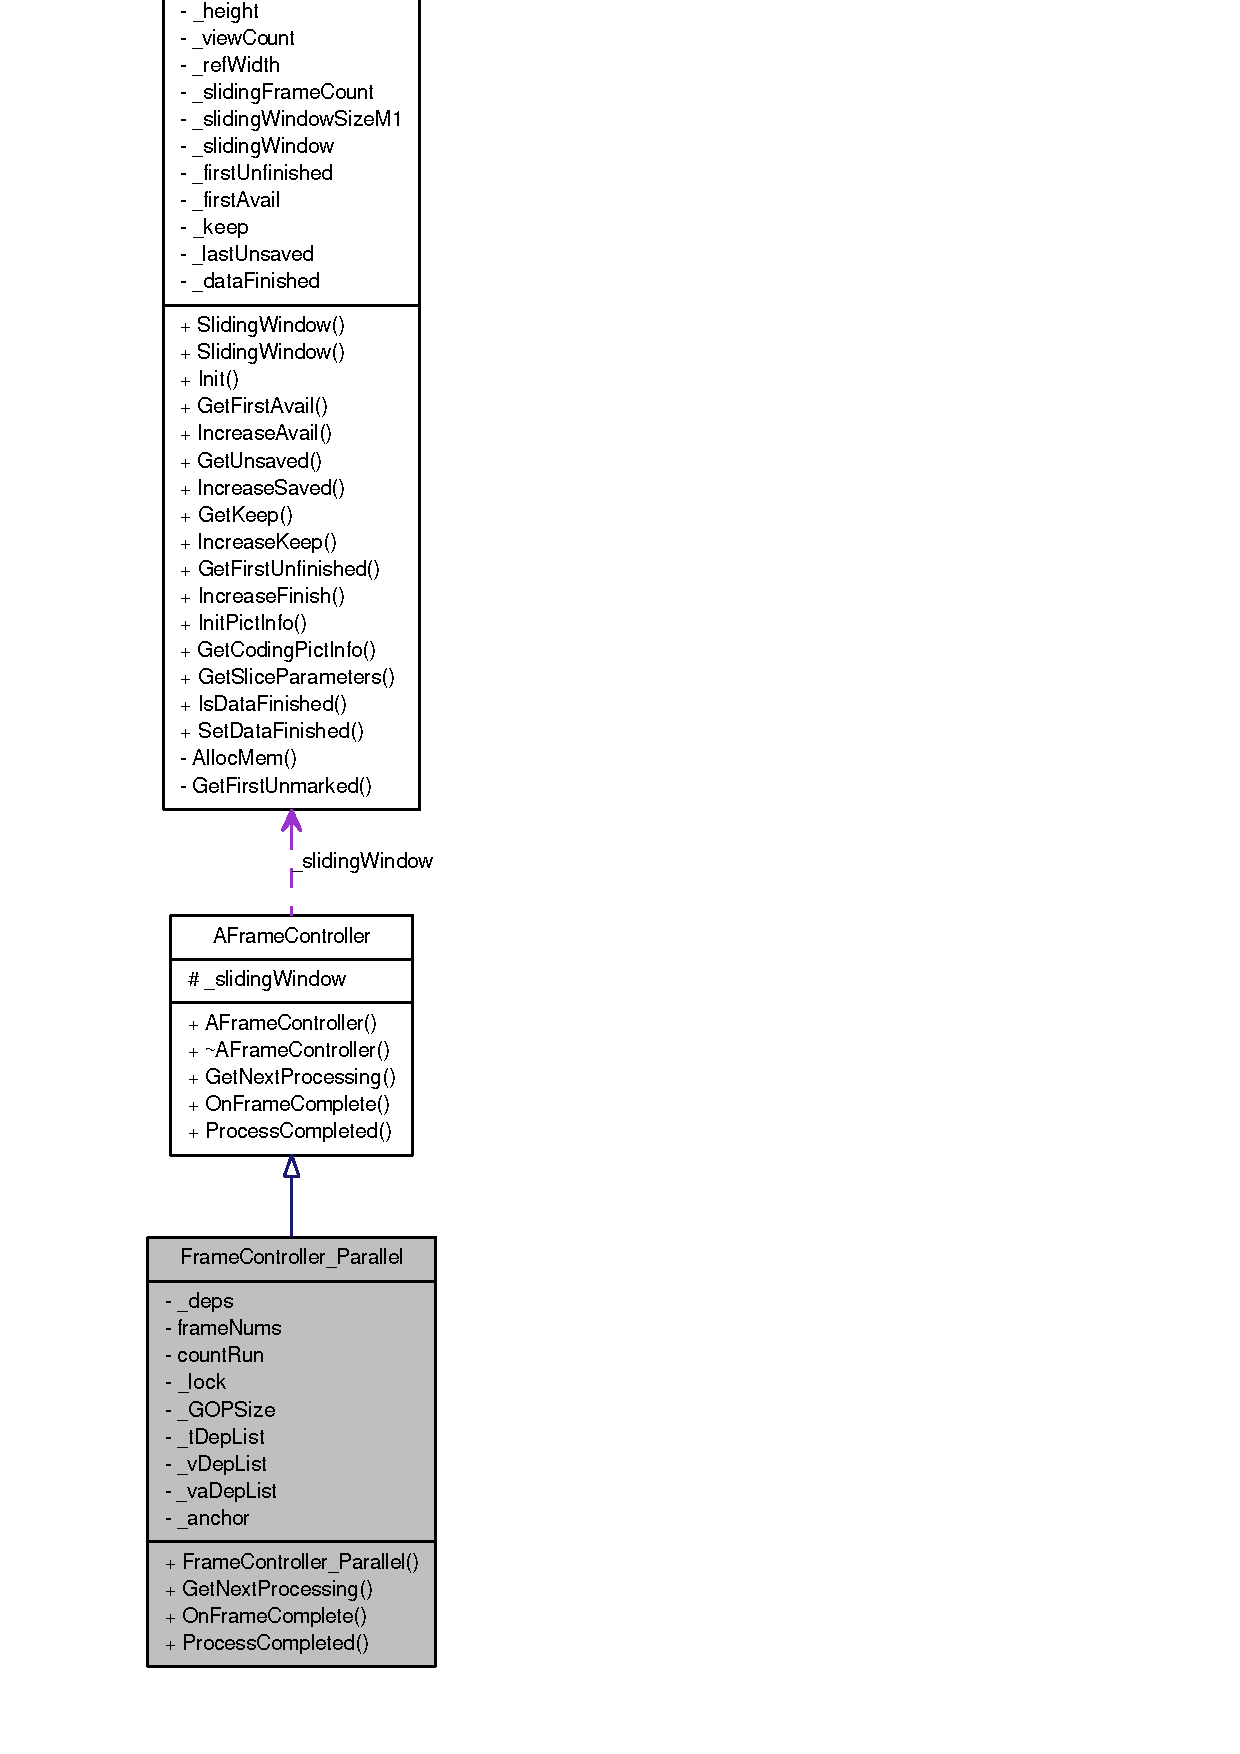
\includegraphics[height=400pt]{class_frame_controller___parallel__coll__graph}
\end{center}
\end{figure}
\subsection*{Public Member Functions}
\begin{DoxyCompactItemize}
\item 
\hyperlink{class_frame_controller___parallel_a5e258e822b7cea0eb61e02b28a7f0db7}{FrameController\_\-Parallel} (\hyperlink{class_sliding_window}{SlidingWindow} $\ast$slidingWindow)
\item 
virtual \hyperlink{struct_coding_pict_info}{CodingPictInfo} $\ast$ \hyperlink{class_frame_controller___parallel_a51792b5fe70db6d99be59c110dbc3041}{GetNextProcessing} ()
\item 
virtual void \hyperlink{class_frame_controller___parallel_a26429e70ddf3aa68cc2d28000a4935e1}{OnFrameComplete} (\hyperlink{struct_coding_pict_info}{CodingPictInfo} $\ast$cpi)
\item 
virtual bool \hyperlink{class_frame_controller___parallel_ac778eb523c6725a9e4da4e4239a88b2a}{ProcessCompleted} ()
\end{DoxyCompactItemize}


\subsection{Constructor \& Destructor Documentation}
\hypertarget{class_frame_controller___parallel_a5e258e822b7cea0eb61e02b28a7f0db7}{
\index{FrameController\_\-Parallel@{FrameController\_\-Parallel}!FrameController\_\-Parallel@{FrameController\_\-Parallel}}
\index{FrameController\_\-Parallel@{FrameController\_\-Parallel}!FrameController_Parallel@{FrameController\_\-Parallel}}
\subsubsection[{FrameController\_\-Parallel}]{\setlength{\rightskip}{0pt plus 5cm}FrameController\_\-Parallel::FrameController\_\-Parallel ({\bf SlidingWindow} $\ast$ {\em slidingWindow})}}
\label{class_frame_controller___parallel_a5e258e822b7cea0eb61e02b28a7f0db7}




\begin{footnotesize}\begin{alltt}
00013                                                                                : 
      \hyperlink{class_a_frame_controller_a448319ad03f91eebc5da7fdf8a43516c}{AFrameController}(slidingWindow)
00014 \{
00015         countRun = 0;
00016 \}
\end{alltt}\end{footnotesize}




\subsection{Member Function Documentation}
\hypertarget{class_frame_controller___parallel_a51792b5fe70db6d99be59c110dbc3041}{
\index{FrameController\_\-Parallel@{FrameController\_\-Parallel}!GetNextProcessing@{GetNextProcessing}}
\index{GetNextProcessing@{GetNextProcessing}!FrameController_Parallel@{FrameController\_\-Parallel}}
\subsubsection[{GetNextProcessing}]{\setlength{\rightskip}{0pt plus 5cm}{\bf CodingPictInfo} $\ast$ FrameController\_\-Parallel::GetNextProcessing ()\hspace{0.3cm}{\ttfamily  \mbox{[}virtual\mbox{]}}}}
\label{class_frame_controller___parallel_a51792b5fe70db6d99be59c110dbc3041}


Implements \hyperlink{class_a_frame_controller_acc142fa10ce535ee171698af719c4d27}{AFrameController}.





\begin{footnotesize}\begin{alltt}
00019 \{
00020         \textcolor{keywordtype}{int} viewCount = \hyperlink{class_codec_info_ad439fd8062a03d868dfe9c9b615b747e}{CodecInfo::GetInstance}().\hyperlink{class_codec_info_aee785011cec77ff3c0c646b498fe1e7d}{sps}.\hyperlink{struct_sequence_parameters_set_af32c7819f630856ccd99aaf78e8f656c}{viewCount};
00021         \_lock.Lock();
00022         \hyperlink{struct_coding_pict_info}{CodingPictInfo} *ret = 0;
00023         \textcolor{keywordtype}{int} proc = \hyperlink{class_a_frame_controller_aca7790494d5c5d114171269ddaabd568}{_slidingWindow}->\hyperlink{class_sliding_window_a3be69abc76bff5b71ab96dadcced9f65}{GetFirstUnfinished}();
00024         \textcolor{keywordtype}{int} avail = \hyperlink{class_a_frame_controller_aca7790494d5c5d114171269ddaabd568}{_slidingWindow}->\hyperlink{class_sliding_window_a2128091c76b407cd0e244759ba5a2846}{GetFirstAvail}();
00025         \textcolor{keywordtype}{int} bi = -1, bj = -1, nref = 100;
00026         \textcolor{keywordflow}{for} (\textcolor{keywordtype}{int} i = proc; !ret && (i < avail); ++i)
00027         \{
00028                 \textcolor{keywordtype}{int} gopOff = i&7;
00029                 \textcolor{keywordtype}{int} gopFirst = i - gopOff;
00030                 \textcolor{keywordflow}{for} (\textcolor{keywordtype}{int} j = 0; j < viewCount; ++j)
00031                 \{
00032                         \hyperlink{struct_coding_pict_info}{CodingPictInfo} *check = \hyperlink{class_a_frame_controller_aca7790494d5c5d114171269ddaabd568}{_slidingWindow}->
      \hyperlink{class_sliding_window_ac50874323a2aaa4ef76fab47f80c9f92}{GetCodingPictInfo}(i, j);
00033                         \textcolor{keywordflow}{if} (!(check->\hyperlink{struct_coding_pict_info_a41498e5ba764405481005e6569d7f728}{pictStatus}&\hyperlink{_picture_info_8h_ade32bc4832afeaeeda7d862a70f2d70d}{PICT_STATUS_PROCESSING}))
00034                         \{
00035                                 \textcolor{keywordtype}{bool} ok = \textcolor{keyword}{true};
00036                                 \textcolor{keywordflow}{for} (\textcolor{keywordtype}{int} depCheck = 0; depCheck < check->
      \hyperlink{struct_coding_pict_info_ab48541faa825385baeca833ffe98b3d4}{Ref_Count}[0]; ++depCheck)
00037                                 \{
00038                                         \textcolor{keywordtype}{int} depTimeId = check->\hyperlink{struct_coding_pict_info_a37079a7e9c26b338a6978063f471a82f}{Ref_Id}[0][depCheck
      ][0],
00039                                                 depViewId = check->\hyperlink{struct_coding_pict_info_a37079a7e9c26b338a6978063f471a82f}{Ref_Id}[0][depC
      heck][1];
00040                                         \hyperlink{struct_coding_pict_info}{CodingPictInfo} *dep = \hyperlink{class_a_frame_controller_aca7790494d5c5d114171269ddaabd568}{_slidingWindow}->
      \hyperlink{class_sliding_window_ac50874323a2aaa4ef76fab47f80c9f92}{GetCodingPictInfo}(depTimeId, depViewId);
00041                                         \textcolor{keywordflow}{if} (!(dep->\hyperlink{struct_coding_pict_info_a41498e5ba764405481005e6569d7f728}{pictStatus}&
      \hyperlink{_picture_info_8h_a170d5962358e97425e08d5646653494b}{PICT_STATUS_FINISHED}))
00042                                         \{
00043                                                 ok = \textcolor{keyword}{false};
00044                                                 \textcolor{keywordflow}{break};
00045                                         \}
00046                                 \}
00047                                 \textcolor{keywordflow}{if} (ok)
00048                                 \{
00049                                         \textcolor{keywordflow}{for} (\textcolor{keywordtype}{int} depCheck = 0; depCheck < check->
      \hyperlink{struct_coding_pict_info_ab48541faa825385baeca833ffe98b3d4}{Ref_Count}[1]; ++depCheck)
00050                                         \{
00051                                                 \textcolor{keywordtype}{int} depTimeId = check->\hyperlink{struct_coding_pict_info_a37079a7e9c26b338a6978063f471a82f}{Ref_Id}[1][
      depCheck][0],
00052                                                         depViewId = check->
      \hyperlink{struct_coding_pict_info_a37079a7e9c26b338a6978063f471a82f}{Ref_Id}[1][depCheck][1];
00053                                                 \hyperlink{struct_coding_pict_info}{CodingPictInfo} *dep = 
      \hyperlink{class_a_frame_controller_aca7790494d5c5d114171269ddaabd568}{_slidingWindow}->\hyperlink{class_sliding_window_ac50874323a2aaa4ef76fab47f80c9f92}{GetCodingPictInfo}(depTimeId, depViewId);
00054                                                 \textcolor{keywordflow}{if} (!(dep->\hyperlink{struct_coding_pict_info_a41498e5ba764405481005e6569d7f728}{pictStatus}&
      \hyperlink{_picture_info_8h_a170d5962358e97425e08d5646653494b}{PICT_STATUS_FINISHED}))
00055                                                 \{
00056                                                         ok = \textcolor{keyword}{false};
00057                                                         \textcolor{keywordflow}{break};
00058                                                 \}
00059                                         \}
00060                                 \}
00061                                 \textcolor{keywordflow}{if} (ok && check->\hyperlink{struct_coding_pict_info_ab48541faa825385baeca833ffe98b3d4}{Ref_Count}[0] + check->\hyperlink{struct_coding_pict_info_ab48541faa825385baeca833ffe98b3d4}{Ref_Count}[
      1] < nref)
00062                                 \{
00063                                         nref = check->\hyperlink{struct_coding_pict_info_ab48541faa825385baeca833ffe98b3d4}{Ref_Count}[0] + check->
      \hyperlink{struct_coding_pict_info_ab48541faa825385baeca833ffe98b3d4}{Ref_Count}[1];
00064                                         bi = i;
00065                                         bj = j;
00066                                 \}
00067                         \}
00068                 \}
00069         \}
00070         \textcolor{keywordflow}{if} (bi!=-1)
00071         \{
00072                 ret = \hyperlink{class_a_frame_controller_aca7790494d5c5d114171269ddaabd568}{_slidingWindow}->\hyperlink{class_sliding_window_ac50874323a2aaa4ef76fab47f80c9f92}{GetCodingPictInfo}(bi, bj);;
00073                 \hyperlink{struct_slice_parameters}{SliceParameters} *sp = \hyperlink{class_a_frame_controller_aca7790494d5c5d114171269ddaabd568}{_slidingWindow}->\hyperlink{class_sliding_window_a020d2c25f1bda31337f91bf9b1a809d1}{GetSliceParameters}(bi, bj);
      
00074                 ret->\hyperlink{struct_coding_pict_info_ad85dae4751165ea3cbb8f7b8c6e61dc3}{timeId} = bi;
00075                 ret->\hyperlink{struct_coding_pict_info_a987595091bfba91b3166b04bca988697}{viewId} = bj;
00076                 ret->\hyperlink{struct_coding_pict_info_a6bfb22b57d0d223546150c71e125fb39}{PictType} = sp->\hyperlink{struct_slice_parameters_a8ab83c948c5e095477d918c0664fce0a}{SliceType};
00077                 ret->\hyperlink{struct_coding_pict_info_a6e808cdf552c3a18da4b75f4d0c35c28}{baseQP} = \hyperlink{class_codec_info_ad439fd8062a03d868dfe9c9b615b747e}{CodecInfo::GetInstance}().\hyperlink{class_codec_info_abaa8d84a7d4045129ee64d91eaac4481}{pps}.\hyperlink{struct_picture_parameters_set_a1c6a508d31929ad84dec0b717ac484a4}{baseQP} + sp->\hyperlink{struct_slice_parameters_a5ca0d343251519b63746af21c1cb9f70}{QP_Delta};
      
00078                 ret->\hyperlink{struct_coding_pict_info_a41498e5ba764405481005e6569d7f728}{pictStatus} |= \hyperlink{_picture_info_8h_ade32bc4832afeaeeda7d862a70f2d70d}{PICT_STATUS_PROCESSING};
00079                 ret->\hyperlink{struct_coding_pict_info_ac290120f5d65f0497efa17928da82922}{log2nFrames} = \hyperlink{class_codec_info_ad439fd8062a03d868dfe9c9b615b747e}{CodecInfo::GetInstance}().\hyperlink{class_codec_info_aee785011cec77ff3c0c646b498fe1e7d}{sps}.\hyperlink{struct_sequence_parameters_set_ac5f0d82a961acfe4f966e7c35aa37339}{log2nFrames};
00080         \}
00081         \_lock.Unlock();
00082         \textcolor{keywordflow}{if} (ret)
00083         \{
00084                 ++countRun;
00085                 \textcolor{comment}{//ret->MP = (NCORE - 1) / countRun + 1;}
00086                 ret->\hyperlink{struct_coding_pict_info_ab254953ed2b4e1de64f05eadbc825646}{MP} = 1;
00087         \}
00088         \textcolor{keywordflow}{return} ret;
00089 \}
\end{alltt}\end{footnotesize}




Here is the call graph for this function:\nopagebreak
\begin{figure}[H]
\begin{center}
\leavevmode
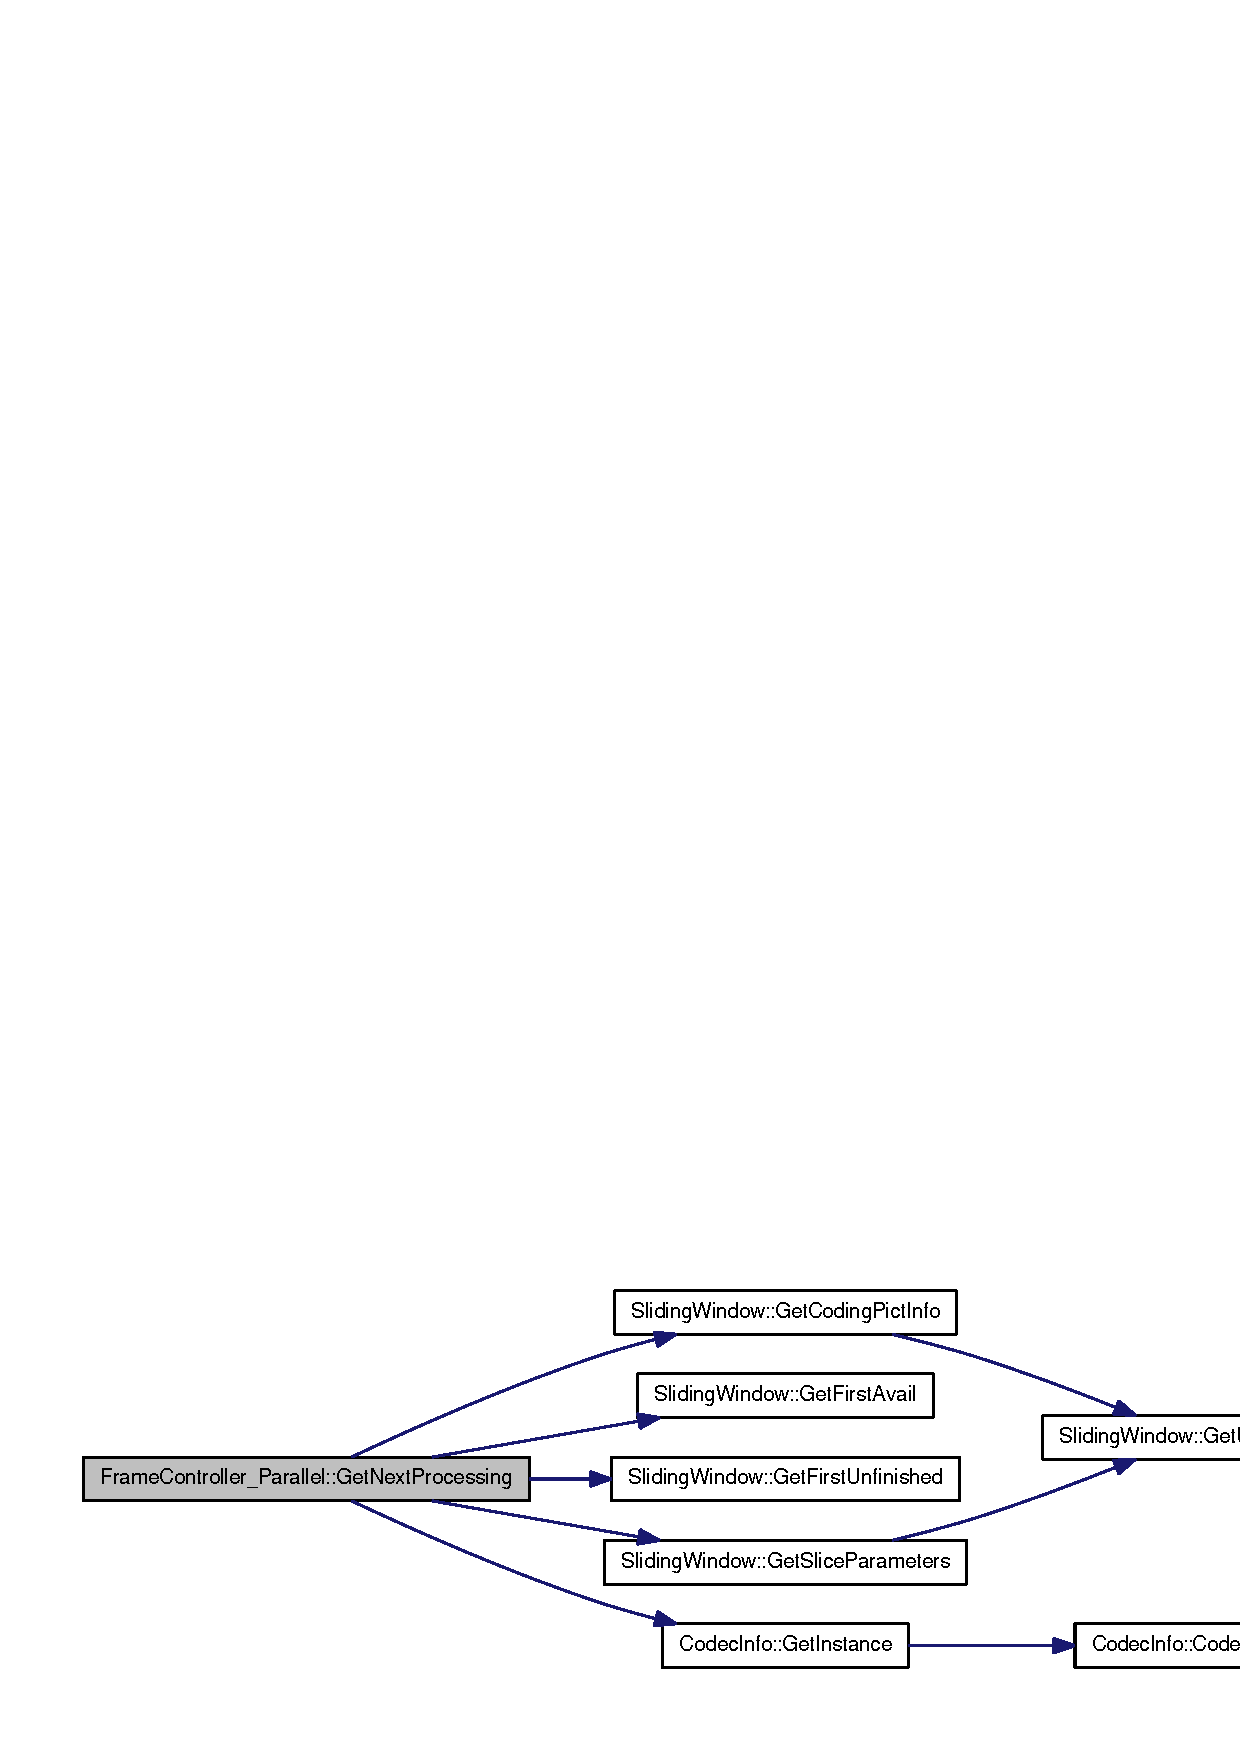
\includegraphics[width=420pt]{class_frame_controller___parallel_a51792b5fe70db6d99be59c110dbc3041_cgraph}
\end{center}
\end{figure}


\hypertarget{class_frame_controller___parallel_a26429e70ddf3aa68cc2d28000a4935e1}{
\index{FrameController\_\-Parallel@{FrameController\_\-Parallel}!OnFrameComplete@{OnFrameComplete}}
\index{OnFrameComplete@{OnFrameComplete}!FrameController_Parallel@{FrameController\_\-Parallel}}
\subsubsection[{OnFrameComplete}]{\setlength{\rightskip}{0pt plus 5cm}void FrameController\_\-Parallel::OnFrameComplete ({\bf CodingPictInfo} $\ast$ {\em cpi})\hspace{0.3cm}{\ttfamily  \mbox{[}virtual\mbox{]}}}}
\label{class_frame_controller___parallel_a26429e70ddf3aa68cc2d28000a4935e1}


Implements \hyperlink{class_a_frame_controller_afd4834463eebfc33536fed009bfb966c}{AFrameController}.





\begin{footnotesize}\begin{alltt}
00092 \{
00093         cpi->\hyperlink{struct_coding_pict_info_a41498e5ba764405481005e6569d7f728}{pictStatus} |= \hyperlink{_picture_info_8h_a170d5962358e97425e08d5646653494b}{PICT_STATUS_FINISHED};
00094         \hyperlink{class_a_frame_controller_aca7790494d5c5d114171269ddaabd568}{_slidingWindow}->\hyperlink{class_sliding_window_a8f303bc211297021f20e09dced119207}{IncreaseFinish}();
00095 \}
\end{alltt}\end{footnotesize}




Here is the call graph for this function:\nopagebreak
\begin{figure}[H]
\begin{center}
\leavevmode
\includegraphics[width=221pt]{class_frame_controller___parallel_a26429e70ddf3aa68cc2d28000a4935e1_cgraph}
\end{center}
\end{figure}


\hypertarget{class_frame_controller___parallel_ac778eb523c6725a9e4da4e4239a88b2a}{
\index{FrameController\_\-Parallel@{FrameController\_\-Parallel}!ProcessCompleted@{ProcessCompleted}}
\index{ProcessCompleted@{ProcessCompleted}!FrameController_Parallel@{FrameController\_\-Parallel}}
\subsubsection[{ProcessCompleted}]{\setlength{\rightskip}{0pt plus 5cm}bool FrameController\_\-Parallel::ProcessCompleted ()\hspace{0.3cm}{\ttfamily  \mbox{[}virtual\mbox{]}}}}
\label{class_frame_controller___parallel_ac778eb523c6725a9e4da4e4239a88b2a}


Implements \hyperlink{class_a_frame_controller_a92ba4b7f8c0c84fff8be7203fae5221d}{AFrameController}.





\begin{footnotesize}\begin{alltt}
00098 \{
00099         \textcolor{keywordflow}{return} \hyperlink{class_a_frame_controller_aca7790494d5c5d114171269ddaabd568}{_slidingWindow}->\hyperlink{class_sliding_window_afd67521d283b68f9fbc769ee9c0ba4b4}{IsDataFinished}() && (\hyperlink{class_a_frame_controller_aca7790494d5c5d114171269ddaabd568}{_slidingWindow}->\hyperlink{class_sliding_window_a3df64e20282ce10a45c4c3f3011e536d}{GetUnsaved}()=
      =\hyperlink{class_a_frame_controller_aca7790494d5c5d114171269ddaabd568}{_slidingWindow}->\hyperlink{class_sliding_window_a2128091c76b407cd0e244759ba5a2846}{GetFirstAvail}());
00100 \}
\end{alltt}\end{footnotesize}




Here is the call graph for this function:\nopagebreak
\begin{figure}[H]
\begin{center}
\leavevmode
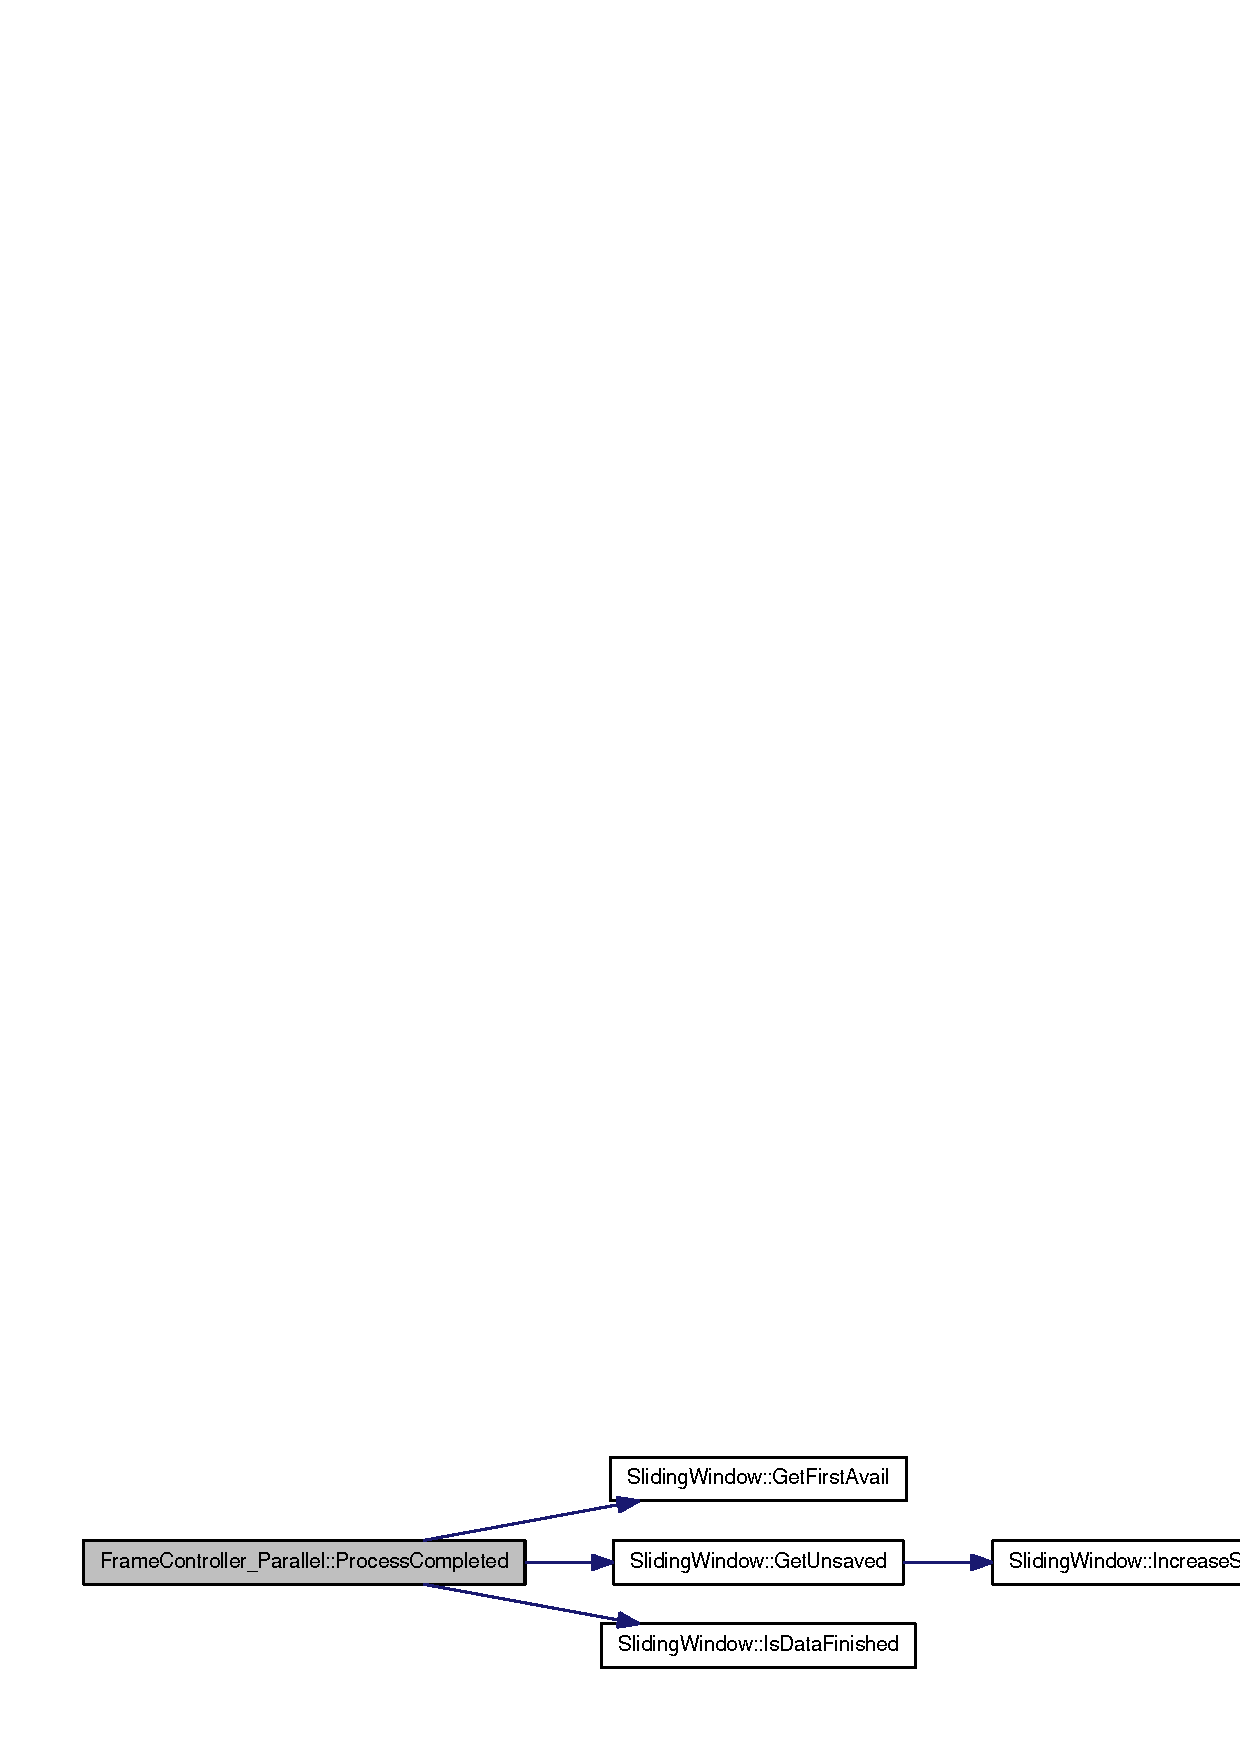
\includegraphics[width=396pt]{class_frame_controller___parallel_ac778eb523c6725a9e4da4e4239a88b2a_cgraph}
\end{center}
\end{figure}




The documentation for this class was generated from the following files:\begin{DoxyCompactItemize}
\item 
MVCDecoder/Controller/\hyperlink{_frame_controller___parallel_8h}{FrameController\_\-Parallel.h}\item 
MVCDecoder/Controller/\hyperlink{_frame_controller___parallel_8cpp}{FrameController\_\-Parallel.cpp}\end{DoxyCompactItemize}

\hypertarget{structhrd__parameters}{
\section{hrd\_\-parameters Struct Reference}
\label{structhrd__parameters}\index{hrd\_\-parameters@{hrd\_\-parameters}}
}


{\ttfamily \#include $<$SequenceParam.h$>$}

\subsection*{Public Attributes}
\begin{DoxyCompactItemize}
\item 
int \hyperlink{structhrd__parameters_a5c6bed7c8fb56f19fcc45d6b48da49af}{cpb\_\-cnt}
\item 
int \hyperlink{structhrd__parameters_ace569254868da81da601fe785961eeab}{bit\_\-rate\_\-scale}
\item 
int \hyperlink{structhrd__parameters_a1609158ce4cbe36e43435936d38b8f59}{cpb\_\-size\_\-scale}
\item 
int \hyperlink{structhrd__parameters_a201add02afdd5156e2559a0420c7ef0f}{bit\_\-rate\_\-value} \mbox{[}32\mbox{]}
\item 
int \hyperlink{structhrd__parameters_a7a2bb5e5dc6c92094669161b33fa5e61}{cpb\_\-size\_\-value} \mbox{[}32\mbox{]}
\item 
bool \hyperlink{structhrd__parameters_aa759c54246d4b4a1ceecc44d56c352c5}{cbr\_\-flag} \mbox{[}32\mbox{]}
\item 
int \hyperlink{structhrd__parameters_a813b2fc9ba06ba6c074610f2469ec2cf}{initial\_\-cpb\_\-removal\_\-delay\_\-length}
\item 
int \hyperlink{structhrd__parameters_a190beef0ba6621955e55235eaa3adf87}{cpb\_\-removal\_\-delay\_\-length}
\item 
int \hyperlink{structhrd__parameters_a5c0bcd60b7cc600016714f0634b8e86c}{dpb\_\-output\_\-delay\_\-length}
\item 
int \hyperlink{structhrd__parameters_a433e874835df091a3754948b51714567}{time\_\-offset}
\end{DoxyCompactItemize}


\subsection{Member Data Documentation}
\hypertarget{structhrd__parameters_ace569254868da81da601fe785961eeab}{
\index{hrd\_\-parameters@{hrd\_\-parameters}!bit\_\-rate\_\-scale@{bit\_\-rate\_\-scale}}
\index{bit\_\-rate\_\-scale@{bit\_\-rate\_\-scale}!hrd_parameters@{hrd\_\-parameters}}
\subsubsection[{bit\_\-rate\_\-scale}]{\setlength{\rightskip}{0pt plus 5cm}int {\bf hrd\_\-parameters::bit\_\-rate\_\-scale}}}
\label{structhrd__parameters_ace569254868da81da601fe785961eeab}
\hypertarget{structhrd__parameters_a201add02afdd5156e2559a0420c7ef0f}{
\index{hrd\_\-parameters@{hrd\_\-parameters}!bit\_\-rate\_\-value@{bit\_\-rate\_\-value}}
\index{bit\_\-rate\_\-value@{bit\_\-rate\_\-value}!hrd_parameters@{hrd\_\-parameters}}
\subsubsection[{bit\_\-rate\_\-value}]{\setlength{\rightskip}{0pt plus 5cm}int {\bf hrd\_\-parameters::bit\_\-rate\_\-value}\mbox{[}32\mbox{]}}}
\label{structhrd__parameters_a201add02afdd5156e2559a0420c7ef0f}
\hypertarget{structhrd__parameters_aa759c54246d4b4a1ceecc44d56c352c5}{
\index{hrd\_\-parameters@{hrd\_\-parameters}!cbr\_\-flag@{cbr\_\-flag}}
\index{cbr\_\-flag@{cbr\_\-flag}!hrd_parameters@{hrd\_\-parameters}}
\subsubsection[{cbr\_\-flag}]{\setlength{\rightskip}{0pt plus 5cm}bool {\bf hrd\_\-parameters::cbr\_\-flag}\mbox{[}32\mbox{]}}}
\label{structhrd__parameters_aa759c54246d4b4a1ceecc44d56c352c5}
\hypertarget{structhrd__parameters_a5c6bed7c8fb56f19fcc45d6b48da49af}{
\index{hrd\_\-parameters@{hrd\_\-parameters}!cpb\_\-cnt@{cpb\_\-cnt}}
\index{cpb\_\-cnt@{cpb\_\-cnt}!hrd_parameters@{hrd\_\-parameters}}
\subsubsection[{cpb\_\-cnt}]{\setlength{\rightskip}{0pt plus 5cm}int {\bf hrd\_\-parameters::cpb\_\-cnt}}}
\label{structhrd__parameters_a5c6bed7c8fb56f19fcc45d6b48da49af}
\hypertarget{structhrd__parameters_a190beef0ba6621955e55235eaa3adf87}{
\index{hrd\_\-parameters@{hrd\_\-parameters}!cpb\_\-removal\_\-delay\_\-length@{cpb\_\-removal\_\-delay\_\-length}}
\index{cpb\_\-removal\_\-delay\_\-length@{cpb\_\-removal\_\-delay\_\-length}!hrd_parameters@{hrd\_\-parameters}}
\subsubsection[{cpb\_\-removal\_\-delay\_\-length}]{\setlength{\rightskip}{0pt plus 5cm}int {\bf hrd\_\-parameters::cpb\_\-removal\_\-delay\_\-length}}}
\label{structhrd__parameters_a190beef0ba6621955e55235eaa3adf87}
\hypertarget{structhrd__parameters_a1609158ce4cbe36e43435936d38b8f59}{
\index{hrd\_\-parameters@{hrd\_\-parameters}!cpb\_\-size\_\-scale@{cpb\_\-size\_\-scale}}
\index{cpb\_\-size\_\-scale@{cpb\_\-size\_\-scale}!hrd_parameters@{hrd\_\-parameters}}
\subsubsection[{cpb\_\-size\_\-scale}]{\setlength{\rightskip}{0pt plus 5cm}int {\bf hrd\_\-parameters::cpb\_\-size\_\-scale}}}
\label{structhrd__parameters_a1609158ce4cbe36e43435936d38b8f59}
\hypertarget{structhrd__parameters_a7a2bb5e5dc6c92094669161b33fa5e61}{
\index{hrd\_\-parameters@{hrd\_\-parameters}!cpb\_\-size\_\-value@{cpb\_\-size\_\-value}}
\index{cpb\_\-size\_\-value@{cpb\_\-size\_\-value}!hrd_parameters@{hrd\_\-parameters}}
\subsubsection[{cpb\_\-size\_\-value}]{\setlength{\rightskip}{0pt plus 5cm}int {\bf hrd\_\-parameters::cpb\_\-size\_\-value}\mbox{[}32\mbox{]}}}
\label{structhrd__parameters_a7a2bb5e5dc6c92094669161b33fa5e61}
\hypertarget{structhrd__parameters_a5c0bcd60b7cc600016714f0634b8e86c}{
\index{hrd\_\-parameters@{hrd\_\-parameters}!dpb\_\-output\_\-delay\_\-length@{dpb\_\-output\_\-delay\_\-length}}
\index{dpb\_\-output\_\-delay\_\-length@{dpb\_\-output\_\-delay\_\-length}!hrd_parameters@{hrd\_\-parameters}}
\subsubsection[{dpb\_\-output\_\-delay\_\-length}]{\setlength{\rightskip}{0pt plus 5cm}int {\bf hrd\_\-parameters::dpb\_\-output\_\-delay\_\-length}}}
\label{structhrd__parameters_a5c0bcd60b7cc600016714f0634b8e86c}
\hypertarget{structhrd__parameters_a813b2fc9ba06ba6c074610f2469ec2cf}{
\index{hrd\_\-parameters@{hrd\_\-parameters}!initial\_\-cpb\_\-removal\_\-delay\_\-length@{initial\_\-cpb\_\-removal\_\-delay\_\-length}}
\index{initial\_\-cpb\_\-removal\_\-delay\_\-length@{initial\_\-cpb\_\-removal\_\-delay\_\-length}!hrd_parameters@{hrd\_\-parameters}}
\subsubsection[{initial\_\-cpb\_\-removal\_\-delay\_\-length}]{\setlength{\rightskip}{0pt plus 5cm}int {\bf hrd\_\-parameters::initial\_\-cpb\_\-removal\_\-delay\_\-length}}}
\label{structhrd__parameters_a813b2fc9ba06ba6c074610f2469ec2cf}
\hypertarget{structhrd__parameters_a433e874835df091a3754948b51714567}{
\index{hrd\_\-parameters@{hrd\_\-parameters}!time\_\-offset@{time\_\-offset}}
\index{time\_\-offset@{time\_\-offset}!hrd_parameters@{hrd\_\-parameters}}
\subsubsection[{time\_\-offset}]{\setlength{\rightskip}{0pt plus 5cm}int {\bf hrd\_\-parameters::time\_\-offset}}}
\label{structhrd__parameters_a433e874835df091a3754948b51714567}


The documentation for this struct was generated from the following file:\begin{DoxyCompactItemize}
\item 
MVCCommonLib/Codec/\hyperlink{_sequence_param_8h}{SequenceParam.h}\end{DoxyCompactItemize}

\hypertarget{class_in_stream}{
\section{InStream Class Reference}
\label{class_in_stream}\index{InStream@{InStream}}
}


{\ttfamily \#include $<$InStream.h$>$}



Collaboration diagram for InStream:\nopagebreak
\begin{figure}[H]
\begin{center}
\leavevmode
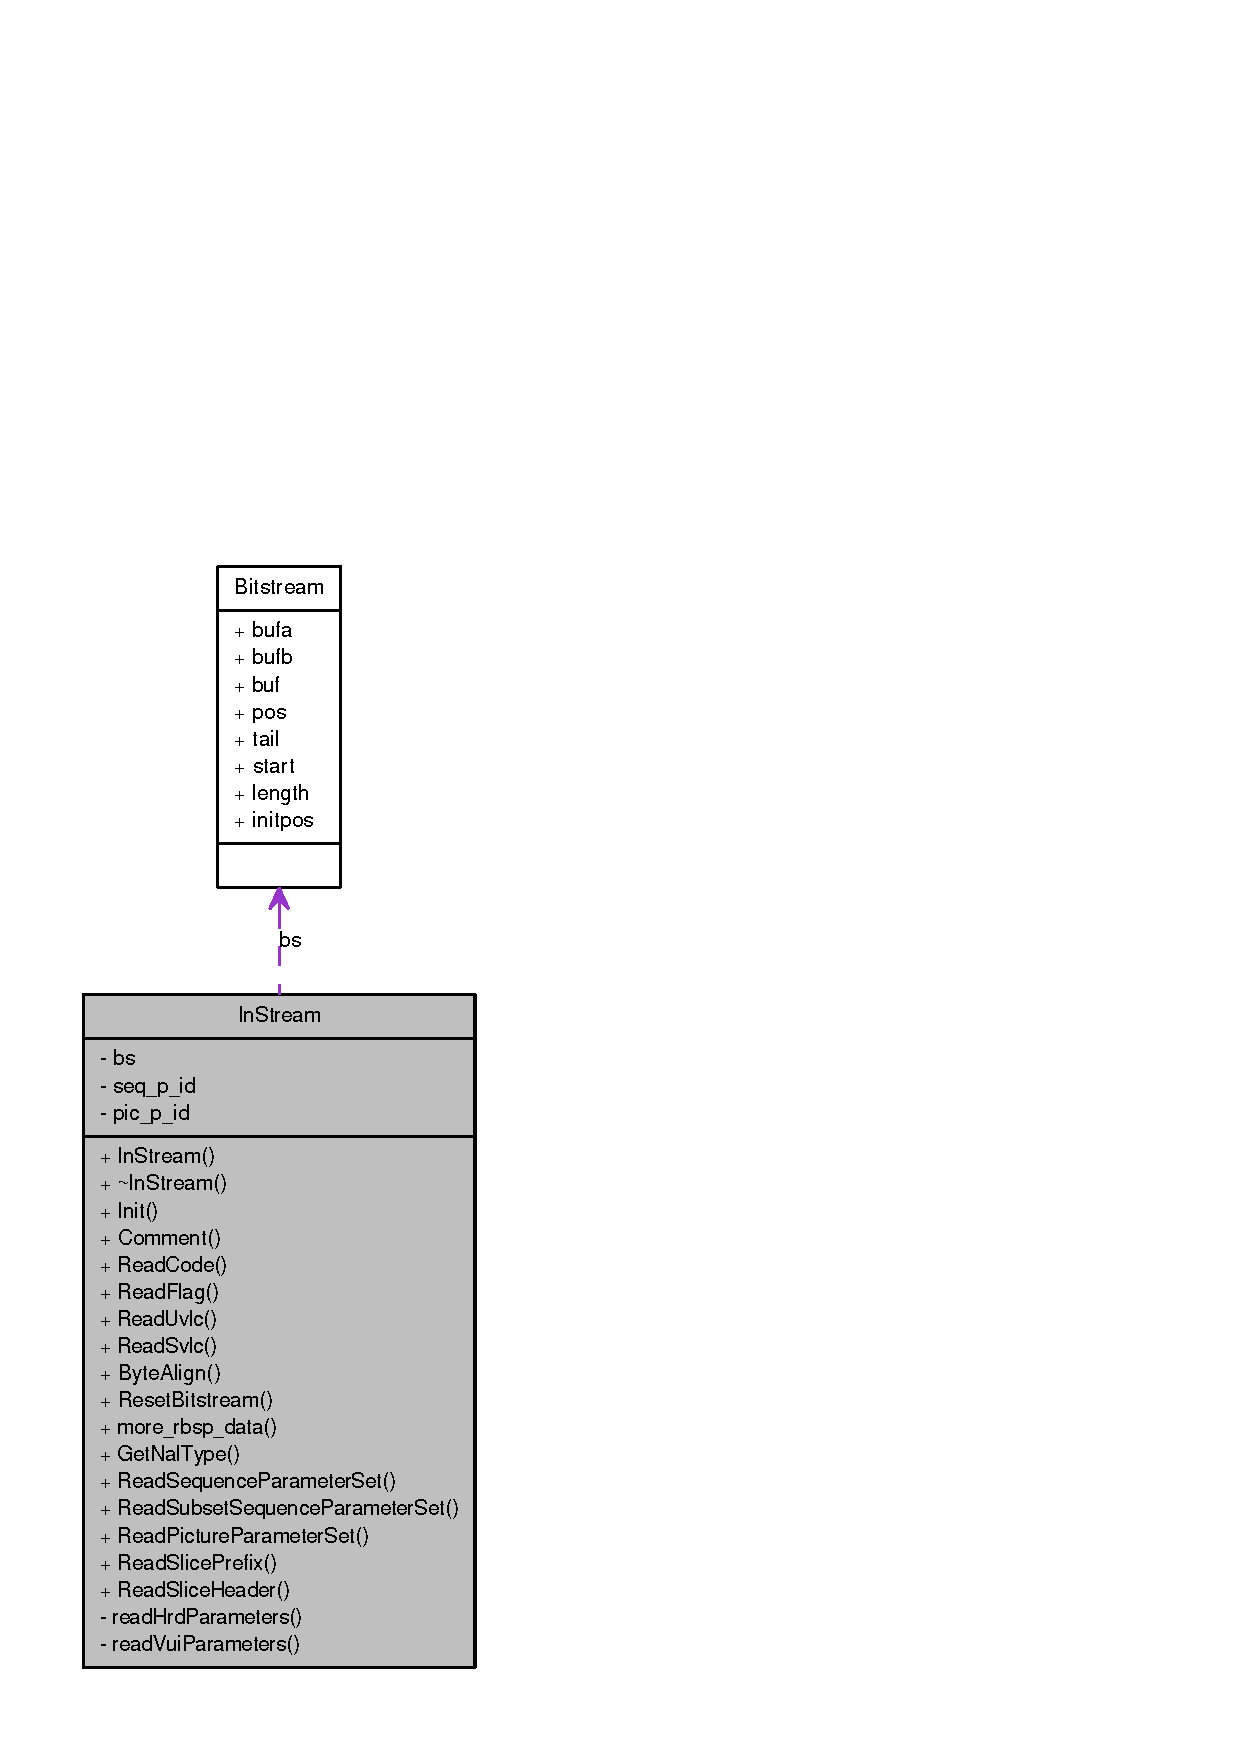
\includegraphics[height=400pt]{class_in_stream__coll__graph}
\end{center}
\end{figure}
\subsection*{Public Member Functions}
\begin{DoxyCompactItemize}
\item 
\hyperlink{class_in_stream_acef728594fc6f21e4b59fa7c37c04057}{InStream} (\hyperlink{_types_8h_a363e4d606232036a6b89060813c45489}{uint8\_\-t} $\ast$buf, int buflen)
\item 
virtual \hyperlink{class_in_stream_ab75c26c4747d2a23388735cdfebbe4fa}{$\sim$InStream} ()
\item 
void \hyperlink{class_in_stream_a299540fd5338ddf57f34b3c6a9df1ebe}{Init} (\hyperlink{_types_8h_a363e4d606232036a6b89060813c45489}{uint8\_\-t} $\ast$buf, int buflen)
\item 
void \hyperlink{class_in_stream_acab96485c6978e95e5ef747ebedf09d6}{Comment} (char $\ast$)
\item 
int \hyperlink{class_in_stream_a07d84696f5dd53b6bbc881dc7507de4c}{ReadCode} (\hyperlink{_types_8h_a04909d1366bb244ff2482beb51635f37}{uint32\_\-t} len)
\item 
int \hyperlink{class_in_stream_a340f8fadf6dfc7d17236b15285bba96f}{ReadFlag} ()
\item 
\hyperlink{_types_8h_a04909d1366bb244ff2482beb51635f37}{uint32\_\-t} \hyperlink{class_in_stream_a8e8daf92cb96e583662cafdaf211093c}{ReadUvlc} ()
\item 
\hyperlink{_types_8h_a115ba3a1b24a8702355c5dbd61ce01e0}{int32\_\-t} \hyperlink{class_in_stream_accc880522e6e43bd3a46297988de1c47}{ReadSvlc} ()
\item 
void \hyperlink{class_in_stream_a27fd3aaea580f6f7eaa5dd7744b9d54d}{ByteAlign} ()
\item 
void \hyperlink{class_in_stream_a700d52a510354fcf7787b118dbeb406f}{ResetBitstream} ()
\item 
bool \hyperlink{class_in_stream_afaa762eba65bc93c673a1cd97d67f812}{more\_\-rbsp\_\-data} ()
\item 
int \hyperlink{class_in_stream_a95ef1b146ee1d6ab6152001fc7719478}{GetNalType} ()
\item 
void \hyperlink{class_in_stream_abaa60d112267ece8de9f303623abd79d}{ReadSequenceParameterSet} (\hyperlink{struct_sequence_parameters_set}{SequenceParametersSet} \&sps)
\item 
void \hyperlink{class_in_stream_abb8e8d2b7eef014e7b6285e130a19a0a}{ReadSubsetSequenceParameterSet} (\hyperlink{struct_sequence_parameters_set}{SequenceParametersSet} \&sps)
\item 
void \hyperlink{class_in_stream_a0f4a6aeef628f4ec90e8ff9ea2e8b566}{ReadPictureParameterSet} (\hyperlink{struct_picture_parameters_set}{PictureParametersSet} \&pps)
\item 
void \hyperlink{class_in_stream_ab40abe55d480a2dc42e484a8a7eb53a4}{ReadSlicePrefix} (\hyperlink{struct_slice_parameters}{SliceParameters} \&sp, const \hyperlink{struct_sequence_parameters_set}{SequenceParametersSet} \&sps)
\item 
int \hyperlink{class_in_stream_a6369ed63c0fad1007f16e3e885825aea}{ReadSliceHeader} (\hyperlink{struct_slice_parameters}{SliceParameters} \&sp, \hyperlink{class_array_list}{ArrayList}$<$ int $>$ $\ast$\&ref\_\-frames, \hyperlink{class_sliding_window}{SlidingWindow} \&slidingWindow, int minTime)
\end{DoxyCompactItemize}


\subsection{Constructor \& Destructor Documentation}
\hypertarget{class_in_stream_acef728594fc6f21e4b59fa7c37c04057}{
\index{InStream@{InStream}!InStream@{InStream}}
\index{InStream@{InStream}!InStream@{InStream}}
\subsubsection[{InStream}]{\setlength{\rightskip}{0pt plus 5cm}InStream::InStream ({\bf uint8\_\-t} $\ast$ {\em buf}, \/  int {\em buflen})}}
\label{class_in_stream_acef728594fc6f21e4b59fa7c37c04057}




\begin{footnotesize}\begin{alltt}
00010                                            : seq\_p\_id(0), pic\_p\_id(0)
00011 \{
00012         BitstreamInit(&bs, buf, buflen);
00013 \}
\end{alltt}\end{footnotesize}


\hypertarget{class_in_stream_ab75c26c4747d2a23388735cdfebbe4fa}{
\index{InStream@{InStream}!$\sim$InStream@{$\sim$InStream}}
\index{$\sim$InStream@{$\sim$InStream}!InStream@{InStream}}
\subsubsection[{$\sim$InStream}]{\setlength{\rightskip}{0pt plus 5cm}InStream::$\sim$InStream ()\hspace{0.3cm}{\ttfamily  \mbox{[}virtual\mbox{]}}}}
\label{class_in_stream_ab75c26c4747d2a23388735cdfebbe4fa}




\begin{footnotesize}\begin{alltt}
00016 \{
00017 \}
\end{alltt}\end{footnotesize}




\subsection{Member Function Documentation}
\hypertarget{class_in_stream_a27fd3aaea580f6f7eaa5dd7744b9d54d}{
\index{InStream@{InStream}!ByteAlign@{ByteAlign}}
\index{ByteAlign@{ByteAlign}!InStream@{InStream}}
\subsubsection[{ByteAlign}]{\setlength{\rightskip}{0pt plus 5cm}void InStream::ByteAlign ()}}
\label{class_in_stream_a27fd3aaea580f6f7eaa5dd7744b9d54d}




\begin{footnotesize}\begin{alltt}
00058 \{
00059         BitstreamByteAlign(&bs);
00060 \}
\end{alltt}\end{footnotesize}


\hypertarget{class_in_stream_acab96485c6978e95e5ef747ebedf09d6}{
\index{InStream@{InStream}!Comment@{Comment}}
\index{Comment@{Comment}!InStream@{InStream}}
\subsubsection[{Comment}]{\setlength{\rightskip}{0pt plus 5cm}void InStream::Comment (char $\ast$ {\em str})}}
\label{class_in_stream_acab96485c6978e95e5ef747ebedf09d6}




\begin{footnotesize}\begin{alltt}
00025 \{
00026         \textcolor{comment}{//printf("%s  ", str);}
00027 \}
\end{alltt}\end{footnotesize}




Here is the caller graph for this function:\nopagebreak
\begin{figure}[H]
\begin{center}
\leavevmode
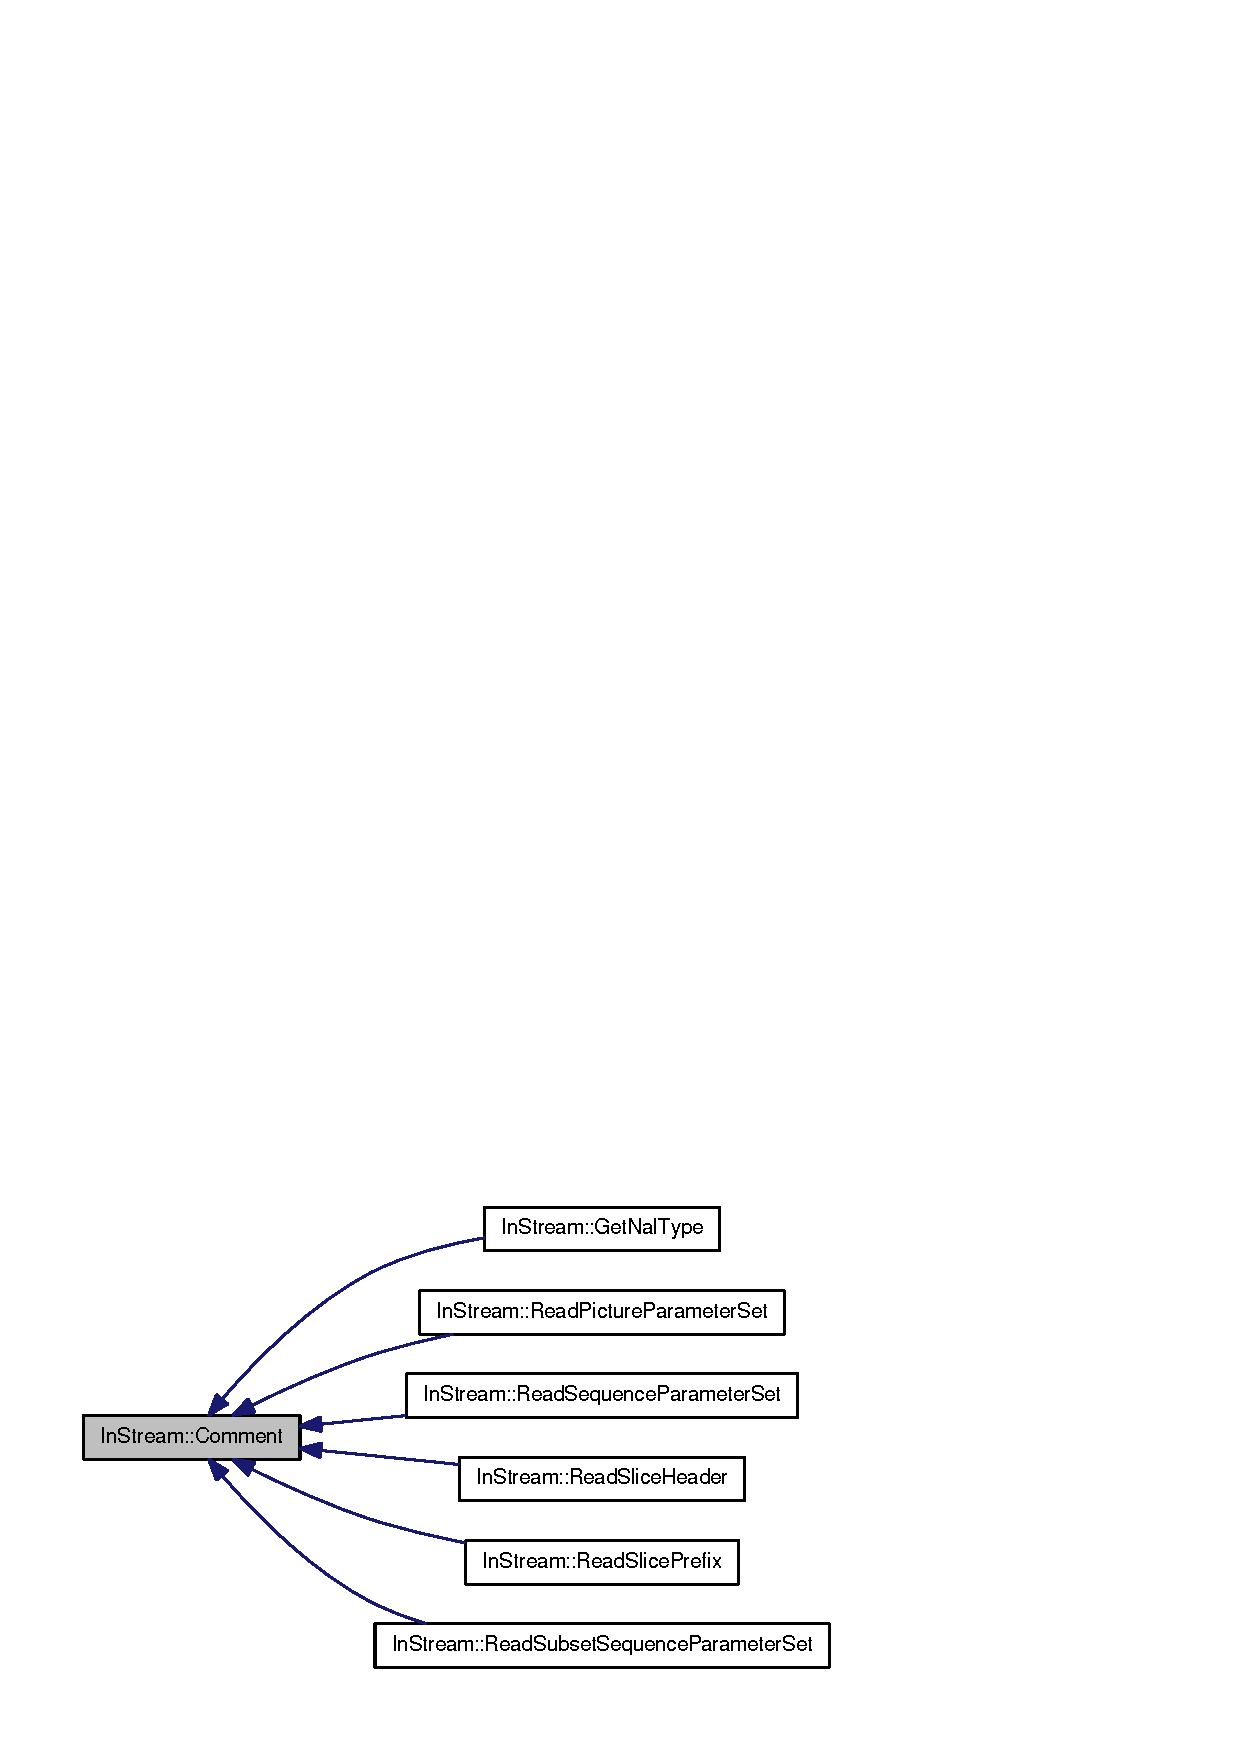
\includegraphics[width=201pt]{class_in_stream_acab96485c6978e95e5ef747ebedf09d6_icgraph}
\end{center}
\end{figure}


\hypertarget{class_in_stream_a95ef1b146ee1d6ab6152001fc7719478}{
\index{InStream@{InStream}!GetNalType@{GetNalType}}
\index{GetNalType@{GetNalType}!InStream@{InStream}}
\subsubsection[{GetNalType}]{\setlength{\rightskip}{0pt plus 5cm}int InStream::GetNalType ()}}
\label{class_in_stream_a95ef1b146ee1d6ab6152001fc7719478}




\begin{footnotesize}\begin{alltt}
00086 \{
00087         \hyperlink{class_in_stream_acab96485c6978e95e5ef747ebedf09d6}{Comment}(\textcolor{stringliteral}{"NALU HEADER: forbidden\_zero\_bit"});
00088         \hyperlink{_debug_8h_a101586fab2b90a8adffe50a3550e235d}{ASSERT}(\hyperlink{class_in_stream_a340f8fadf6dfc7d17236b15285bba96f}{ReadFlag}() == 0);
00089         \hyperlink{class_in_stream_acab96485c6978e95e5ef747ebedf09d6}{Comment}(\textcolor{stringliteral}{"NALU HEADER: nal\_ref\_idc"});
00090         \hyperlink{class_in_stream_a07d84696f5dd53b6bbc881dc7507de4c}{ReadCode}(2);
00091         \hyperlink{class_in_stream_acab96485c6978e95e5ef747ebedf09d6}{Comment}(\textcolor{stringliteral}{"NALU HEADER: nal\_unit\_type"});
00092         \textcolor{keywordtype}{int} ret = \hyperlink{class_in_stream_a07d84696f5dd53b6bbc881dc7507de4c}{ReadCode}(5);
00093         \hyperlink{class_in_stream_a700d52a510354fcf7787b118dbeb406f}{ResetBitstream}();
00094         \textcolor{keywordflow}{return} ret;
00095 \}
\end{alltt}\end{footnotesize}




Here is the call graph for this function:\nopagebreak
\begin{figure}[H]
\begin{center}
\leavevmode
\includegraphics[width=162pt]{class_in_stream_a95ef1b146ee1d6ab6152001fc7719478_cgraph}
\end{center}
\end{figure}


\hypertarget{class_in_stream_a299540fd5338ddf57f34b3c6a9df1ebe}{
\index{InStream@{InStream}!Init@{Init}}
\index{Init@{Init}!InStream@{InStream}}
\subsubsection[{Init}]{\setlength{\rightskip}{0pt plus 5cm}void InStream::Init ({\bf uint8\_\-t} $\ast$ {\em buf}, \/  int {\em buflen})}}
\label{class_in_stream_a299540fd5338ddf57f34b3c6a9df1ebe}




\begin{footnotesize}\begin{alltt}
00020 \{
00021         BitstreamInit(&bs, buf, buflen);
00022 \}
\end{alltt}\end{footnotesize}


\hypertarget{class_in_stream_afaa762eba65bc93c673a1cd97d67f812}{
\index{InStream@{InStream}!more\_\-rbsp\_\-data@{more\_\-rbsp\_\-data}}
\index{more\_\-rbsp\_\-data@{more\_\-rbsp\_\-data}!InStream@{InStream}}
\subsubsection[{more\_\-rbsp\_\-data}]{\setlength{\rightskip}{0pt plus 5cm}bool InStream::more\_\-rbsp\_\-data ()}}
\label{class_in_stream_afaa762eba65bc93c673a1cd97d67f812}




\begin{footnotesize}\begin{alltt}
00068 \{
00069         \hyperlink{_types_8h_a115ba3a1b24a8702355c5dbd61ce01e0}{int32_t} pos = BitstreamPos(&bs);
00070         \hyperlink{_types_8h_a115ba3a1b24a8702355c5dbd61ce01e0}{int32_t} len = bs.\hyperlink{struct_bitstream_a56ea589bea2ad26a4512ff556b055fd8}{length} * 8;
00071         \hyperlink{_types_8h_a363e4d606232036a6b89060813c45489}{uint8_t} last = ((\hyperlink{_types_8h_adde6aaee8457bee49c2a92621fe22b79}{uint8}*)bs.\hyperlink{struct_bitstream_a4c2cb09a4fee7ed90d05f8b40914911e}{start})[bs.\hyperlink{struct_bitstream_a56ea589bea2ad26a4512ff556b055fd8}{length}-1];
00072         \textcolor{keywordflow}{if} (last==0)
00073                 len-=8;
00074         \textcolor{keywordflow}{else}
00075         \{
00076                 \textcolor{keywordflow}{while} (!(last&1))
00077                 \{
00078                         last>>=1;
00079                         --len;
00080                 \}
00081         \}
00082         \textcolor{keywordflow}{return} pos<len-1;
00083 \}
\end{alltt}\end{footnotesize}




Here is the caller graph for this function:\nopagebreak
\begin{figure}[H]
\begin{center}
\leavevmode
\includegraphics[width=194pt]{class_in_stream_afaa762eba65bc93c673a1cd97d67f812_icgraph}
\end{center}
\end{figure}


\hypertarget{class_in_stream_a07d84696f5dd53b6bbc881dc7507de4c}{
\index{InStream@{InStream}!ReadCode@{ReadCode}}
\index{ReadCode@{ReadCode}!InStream@{InStream}}
\subsubsection[{ReadCode}]{\setlength{\rightskip}{0pt plus 5cm}int InStream::ReadCode ({\bf uint32\_\-t} {\em len})}}
\label{class_in_stream_a07d84696f5dd53b6bbc881dc7507de4c}




\begin{footnotesize}\begin{alltt}
00030 \{
00031         \textcolor{keywordtype}{int} code = \hyperlink{_bitstream_8h_a3474bd178129247b388e870a0bd602a3}{eg_read_direct}(&bs, len);
00032         \textcolor{comment}{//printf("Code %08lX, %d\(\backslash\)n", code, len);}
00033         \textcolor{keywordflow}{return} code;
00034 \}
\end{alltt}\end{footnotesize}




Here is the caller graph for this function:\nopagebreak
\begin{figure}[H]
\begin{center}
\leavevmode
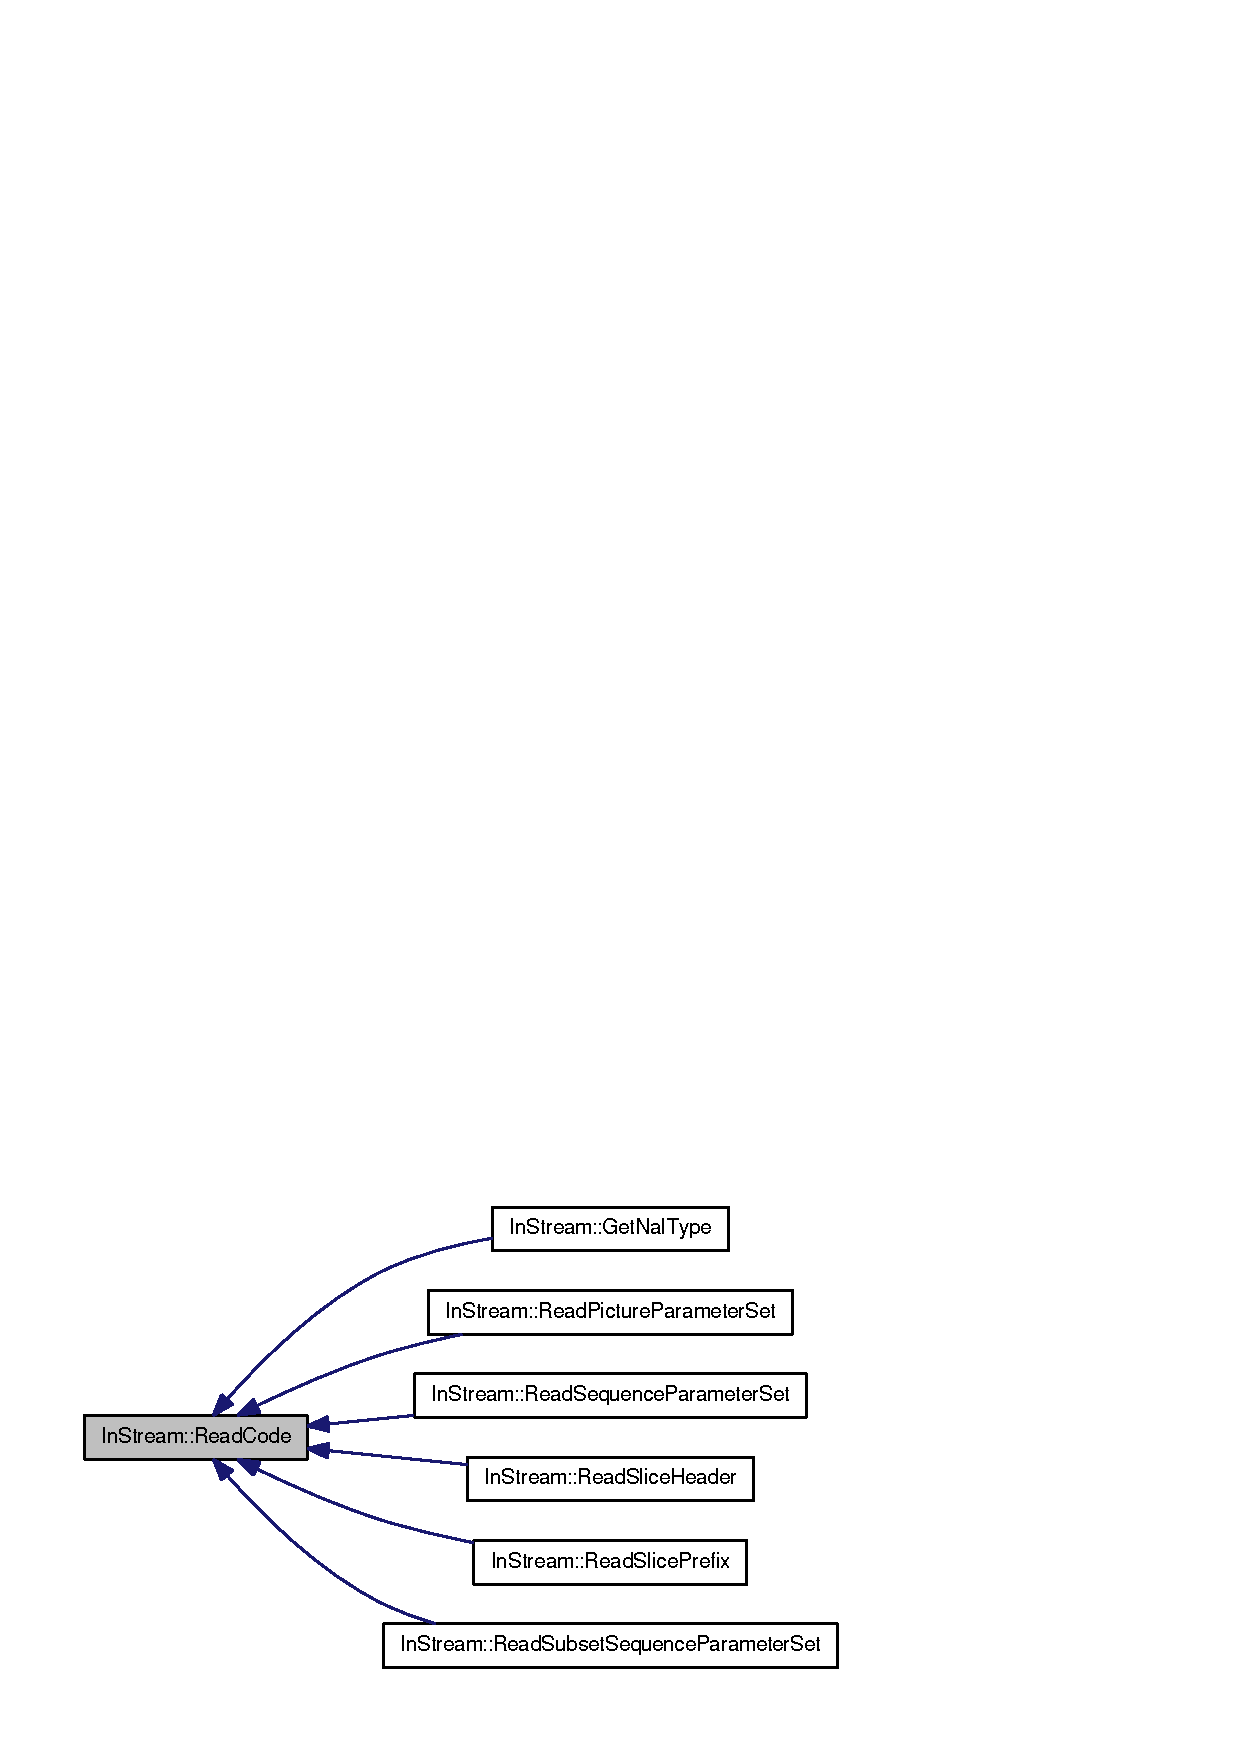
\includegraphics[width=203pt]{class_in_stream_a07d84696f5dd53b6bbc881dc7507de4c_icgraph}
\end{center}
\end{figure}


\hypertarget{class_in_stream_a340f8fadf6dfc7d17236b15285bba96f}{
\index{InStream@{InStream}!ReadFlag@{ReadFlag}}
\index{ReadFlag@{ReadFlag}!InStream@{InStream}}
\subsubsection[{ReadFlag}]{\setlength{\rightskip}{0pt plus 5cm}int InStream::ReadFlag ()}}
\label{class_in_stream_a340f8fadf6dfc7d17236b15285bba96f}




\begin{footnotesize}\begin{alltt}
00037 \{
00038         \textcolor{keywordtype}{int} code = \hyperlink{_bitstream_8h_a930f8a3acc36d15b74015dd4579f485c}{eg_read_direct1}(&bs);
00039         \textcolor{comment}{//printf("Flag %d\(\backslash\)n", code);}
00040         \textcolor{keywordflow}{return} code;
00041 \}
\end{alltt}\end{footnotesize}




Here is the caller graph for this function:\nopagebreak
\begin{figure}[H]
\begin{center}
\leavevmode
\includegraphics[width=201pt]{class_in_stream_a340f8fadf6dfc7d17236b15285bba96f_icgraph}
\end{center}
\end{figure}


\hypertarget{class_in_stream_a0f4a6aeef628f4ec90e8ff9ea2e8b566}{
\index{InStream@{InStream}!ReadPictureParameterSet@{ReadPictureParameterSet}}
\index{ReadPictureParameterSet@{ReadPictureParameterSet}!InStream@{InStream}}
\subsubsection[{ReadPictureParameterSet}]{\setlength{\rightskip}{0pt plus 5cm}void InStream::ReadPictureParameterSet ({\bf PictureParametersSet} \& {\em pps})}}
\label{class_in_stream_a0f4a6aeef628f4ec90e8ff9ea2e8b566}




\begin{footnotesize}\begin{alltt}
00495 \{
00496         \hyperlink{class_in_stream_acab96485c6978e95e5ef747ebedf09d6}{Comment}(\textcolor{stringliteral}{"NALU HEADER: forbidden\_zero\_bit"});
00497         \hyperlink{_debug_8h_a101586fab2b90a8adffe50a3550e235d}{ASSERT}(\hyperlink{class_in_stream_a340f8fadf6dfc7d17236b15285bba96f}{ReadFlag}() == 0);
00498         \hyperlink{class_in_stream_acab96485c6978e95e5ef747ebedf09d6}{Comment}(\textcolor{stringliteral}{"NALU HEADER: nal\_ref\_idc"});
00499         \hyperlink{_debug_8h_a101586fab2b90a8adffe50a3550e235d}{ASSERT}(\hyperlink{class_in_stream_a07d84696f5dd53b6bbc881dc7507de4c}{ReadCode}(2) == 3);
00500         \hyperlink{class_in_stream_acab96485c6978e95e5ef747ebedf09d6}{Comment}(\textcolor{stringliteral}{"NALU HEADER: nal\_unit\_type"});
00501         \hyperlink{_debug_8h_a101586fab2b90a8adffe50a3550e235d}{ASSERT}(\hyperlink{class_in_stream_a07d84696f5dd53b6bbc881dc7507de4c}{ReadCode}(5) == \hyperlink{_consts4_standard_8h_a0ae628337fb17a2b11855dd3524f3d04a0a937a1dcddd0ed49b7bbcc120a0a800}{NAL_UNIT_PPS});
00502 
00503         \hyperlink{class_in_stream_acab96485c6978e95e5ef747ebedf09d6}{Comment}(\textcolor{stringliteral}{"PPS: pic\_parameter\_set\_id"});
00504         \hyperlink{class_in_stream_a8e8daf92cb96e583662cafdaf211093c}{ReadUvlc}();
00505         \hyperlink{class_in_stream_acab96485c6978e95e5ef747ebedf09d6}{Comment}(\textcolor{stringliteral}{"PPS: seq\_parameter\_set\_id"});
00506         \hyperlink{class_in_stream_a8e8daf92cb96e583662cafdaf211093c}{ReadUvlc}();
00507         \hyperlink{class_in_stream_acab96485c6978e95e5ef747ebedf09d6}{Comment}(\textcolor{stringliteral}{"PPS: entropy\_coding\_mode\_flag"});
00508         \hyperlink{_debug_8h_a101586fab2b90a8adffe50a3550e235d}{ASSERT}(\hyperlink{class_in_stream_a340f8fadf6dfc7d17236b15285bba96f}{ReadFlag}() == 0);
00509         \hyperlink{class_in_stream_acab96485c6978e95e5ef747ebedf09d6}{Comment}(\textcolor{stringliteral}{"PPS: pic\_order\_present\_flag"});
00510         pps.\hyperlink{struct_picture_parameters_set_a9611d788502cf2646a1fafd8f1cc7e4f}{pic_order_present_flag} = (\hyperlink{class_in_stream_a340f8fadf6dfc7d17236b15285bba96f}{ReadFlag}() == 1);
00511 
00512         \hyperlink{class_in_stream_acab96485c6978e95e5ef747ebedf09d6}{Comment}(\textcolor{stringliteral}{"PPS: num\_slice\_groups\_minus1"});
00513         \hyperlink{_debug_8h_a101586fab2b90a8adffe50a3550e235d}{ASSERT}(\hyperlink{class_in_stream_a8e8daf92cb96e583662cafdaf211093c}{ReadUvlc}() == 0);
00514 
00515         \hyperlink{class_in_stream_acab96485c6978e95e5ef747ebedf09d6}{Comment}(\textcolor{stringliteral}{"PPS: num\_ref\_idx\_l0\_active\_minus1"});
00516         pps.\hyperlink{struct_picture_parameters_set_abc9eb8dcb637bef8a76a7c12380fccf9}{num_ref_idx_l0_active} = \hyperlink{class_in_stream_a8e8daf92cb96e583662cafdaf211093c}{ReadUvlc}() + 1;
00517         \hyperlink{class_in_stream_acab96485c6978e95e5ef747ebedf09d6}{Comment}(\textcolor{stringliteral}{"PPS: num\_ref\_idx\_l1\_active\_minus1"});
00518         pps.\hyperlink{struct_picture_parameters_set_afb1dc1e024b6c9263e33d3f1dd233203}{num_ref_idx_l1_active} = \hyperlink{class_in_stream_a8e8daf92cb96e583662cafdaf211093c}{ReadUvlc}() + 1;
00519         \hyperlink{class_in_stream_acab96485c6978e95e5ef747ebedf09d6}{Comment}(\textcolor{stringliteral}{"PPS: weighted\_pred\_flag"});
00520         pps.\hyperlink{struct_picture_parameters_set_a4cd484fee6229fd37fa2bf7519458f3a}{weighted_pred_flag} = \hyperlink{class_in_stream_a340f8fadf6dfc7d17236b15285bba96f}{ReadFlag}();
00521         \hyperlink{_debug_8h_a101586fab2b90a8adffe50a3550e235d}{ASSERT}(pps.\hyperlink{struct_picture_parameters_set_a4cd484fee6229fd37fa2bf7519458f3a}{weighted_pred_flag}==0);
00522         \hyperlink{class_in_stream_acab96485c6978e95e5ef747ebedf09d6}{Comment}(\textcolor{stringliteral}{"PPS: weighted\_bipred\_idc"});
00523         pps.\hyperlink{struct_picture_parameters_set_a436591953af7e22c28e0e2844acdf9f3}{weighted_bipred_idc} = \hyperlink{class_in_stream_a07d84696f5dd53b6bbc881dc7507de4c}{ReadCode}(2);
00524         \hyperlink{_debug_8h_a101586fab2b90a8adffe50a3550e235d}{ASSERT}(pps.\hyperlink{struct_picture_parameters_set_a436591953af7e22c28e0e2844acdf9f3}{weighted_bipred_idc}==0);
00525         \hyperlink{class_in_stream_acab96485c6978e95e5ef747ebedf09d6}{Comment}(\textcolor{stringliteral}{"PPS: pic\_init\_qp\_minus26"});
00526         pps.\hyperlink{struct_picture_parameters_set_a1c6a508d31929ad84dec0b717ac484a4}{baseQP} = \hyperlink{class_in_stream_accc880522e6e43bd3a46297988de1c47}{ReadSvlc}() + 26;
00527         \hyperlink{class_in_stream_acab96485c6978e95e5ef747ebedf09d6}{Comment}(\textcolor{stringliteral}{"PPS: pic\_init\_qs\_minus26"});
00528         \hyperlink{_debug_8h_a101586fab2b90a8adffe50a3550e235d}{ASSERT}(\hyperlink{class_in_stream_accc880522e6e43bd3a46297988de1c47}{ReadSvlc}() == 0);
00529         \hyperlink{class_in_stream_acab96485c6978e95e5ef747ebedf09d6}{Comment}(\textcolor{stringliteral}{"PPS: chroma\_qp\_index\_offset"});
00530         \hyperlink{_debug_8h_a101586fab2b90a8adffe50a3550e235d}{ASSERT}(\hyperlink{class_in_stream_accc880522e6e43bd3a46297988de1c47}{ReadSvlc}() == 0);
00531         \hyperlink{class_in_stream_acab96485c6978e95e5ef747ebedf09d6}{Comment}(\textcolor{stringliteral}{"PPS: deblocking\_filter\_parameters\_present\_flag"});
00532         \hyperlink{_debug_8h_a101586fab2b90a8adffe50a3550e235d}{ASSERT}(\hyperlink{class_in_stream_a340f8fadf6dfc7d17236b15285bba96f}{ReadFlag}() == 0);
00533         \hyperlink{class_in_stream_acab96485c6978e95e5ef747ebedf09d6}{Comment}(\textcolor{stringliteral}{"PPS: constrained\_intra\_pred\_flag"});
00534         \hyperlink{_debug_8h_a101586fab2b90a8adffe50a3550e235d}{ASSERT}(\hyperlink{class_in_stream_a340f8fadf6dfc7d17236b15285bba96f}{ReadFlag}() == 0);
00535         \hyperlink{class_in_stream_acab96485c6978e95e5ef747ebedf09d6}{Comment}(\textcolor{stringliteral}{"PPS: redundant\_pic\_cnt\_present\_flag"});
00536         \hyperlink{_debug_8h_a101586fab2b90a8adffe50a3550e235d}{ASSERT}(\hyperlink{class_in_stream_a340f8fadf6dfc7d17236b15285bba96f}{ReadFlag}() == 0);
00537 
00538         \textcolor{keywordflow}{if} (\hyperlink{class_in_stream_afaa762eba65bc93c673a1cd97d67f812}{more_rbsp_data}())
00539         \{
00540                 \hyperlink{class_in_stream_acab96485c6978e95e5ef747ebedf09d6}{Comment}(\textcolor{stringliteral}{"PPS: transform\_8x8\_mode\_flag"});
00541                 \hyperlink{_debug_8h_a101586fab2b90a8adffe50a3550e235d}{ASSERT}(\hyperlink{class_in_stream_a340f8fadf6dfc7d17236b15285bba96f}{ReadFlag}() == 1);
00542                 \hyperlink{class_in_stream_acab96485c6978e95e5ef747ebedf09d6}{Comment}(\textcolor{stringliteral}{"PPS: pic\_scaling\_matrix\_present\_flag"});
00543                 \hyperlink{_debug_8h_a101586fab2b90a8adffe50a3550e235d}{ASSERT}(\hyperlink{class_in_stream_a340f8fadf6dfc7d17236b15285bba96f}{ReadFlag}() == 0);
00544                 \hyperlink{class_in_stream_acab96485c6978e95e5ef747ebedf09d6}{Comment}(\textcolor{stringliteral}{"PPS: second\_chroma\_qp\_index\_offset"});
00545                 \hyperlink{_debug_8h_a101586fab2b90a8adffe50a3550e235d}{ASSERT}(\hyperlink{class_in_stream_accc880522e6e43bd3a46297988de1c47}{ReadSvlc}() == 0);
00546         \}
00547 \}
\end{alltt}\end{footnotesize}




Here is the call graph for this function:\nopagebreak
\begin{figure}[H]
\begin{center}
\leavevmode
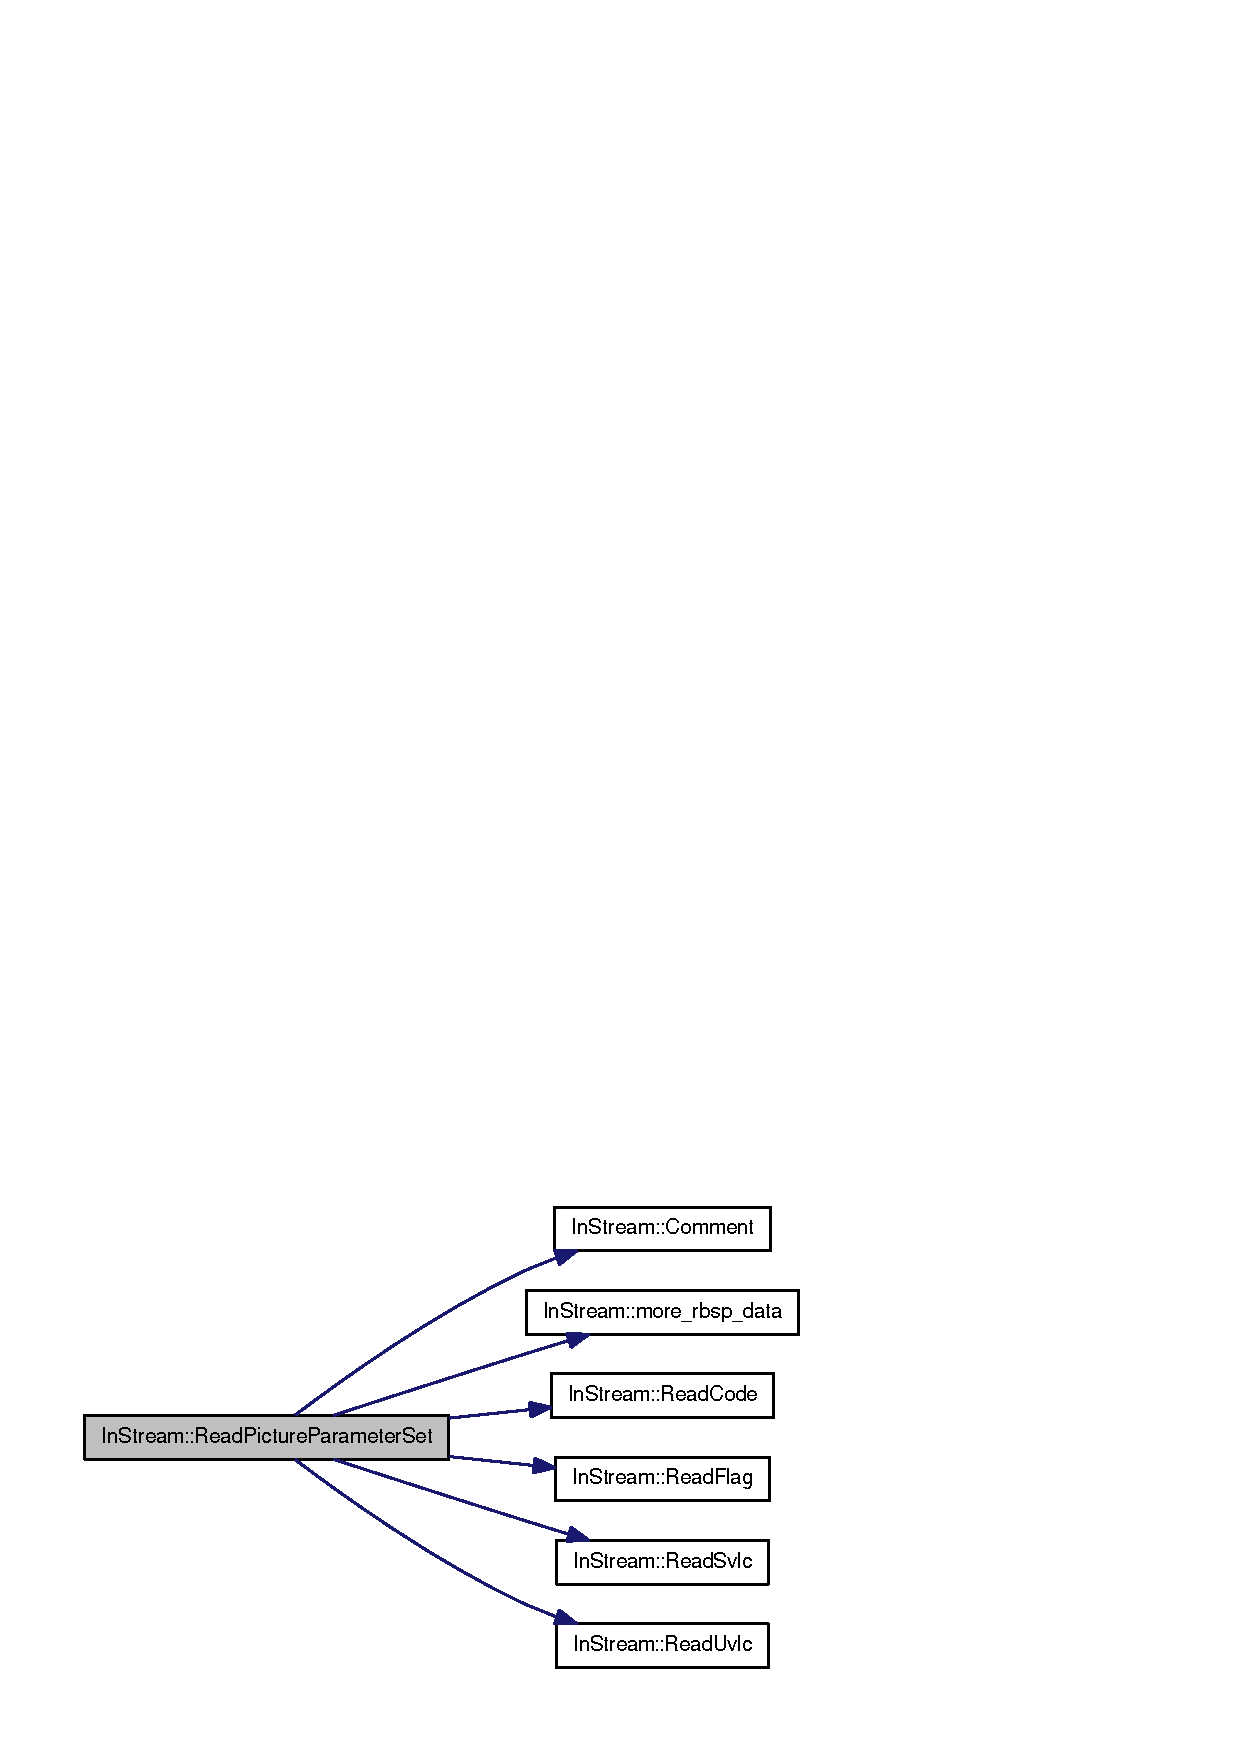
\includegraphics[width=194pt]{class_in_stream_a0f4a6aeef628f4ec90e8ff9ea2e8b566_cgraph}
\end{center}
\end{figure}


\hypertarget{class_in_stream_abaa60d112267ece8de9f303623abd79d}{
\index{InStream@{InStream}!ReadSequenceParameterSet@{ReadSequenceParameterSet}}
\index{ReadSequenceParameterSet@{ReadSequenceParameterSet}!InStream@{InStream}}
\subsubsection[{ReadSequenceParameterSet}]{\setlength{\rightskip}{0pt plus 5cm}void InStream::ReadSequenceParameterSet ({\bf SequenceParametersSet} \& {\em sps})}}
\label{class_in_stream_abaa60d112267ece8de9f303623abd79d}




\begin{footnotesize}\begin{alltt}
00229 \{
00230         \hyperlink{class_in_stream_acab96485c6978e95e5ef747ebedf09d6}{Comment}(\textcolor{stringliteral}{"NALU HEADER: forbidden\_zero\_bit"});
00231         \hyperlink{_debug_8h_a101586fab2b90a8adffe50a3550e235d}{ASSERT}(\hyperlink{class_in_stream_a340f8fadf6dfc7d17236b15285bba96f}{ReadFlag}() == 0);
00232         \hyperlink{class_in_stream_acab96485c6978e95e5ef747ebedf09d6}{Comment}(\textcolor{stringliteral}{"NALU HEADER: nal\_ref\_idc"});
00233         \hyperlink{_debug_8h_a101586fab2b90a8adffe50a3550e235d}{ASSERT}(\hyperlink{class_in_stream_a07d84696f5dd53b6bbc881dc7507de4c}{ReadCode}(2) == 3);
00234         \hyperlink{class_in_stream_acab96485c6978e95e5ef747ebedf09d6}{Comment}(\textcolor{stringliteral}{"NALU HEADER: nal\_unit\_type"});
00235         \hyperlink{_debug_8h_a101586fab2b90a8adffe50a3550e235d}{ASSERT}(\hyperlink{class_in_stream_a07d84696f5dd53b6bbc881dc7507de4c}{ReadCode}(5) == \hyperlink{_consts4_standard_8h_a0ae628337fb17a2b11855dd3524f3d04a87cac3a362213e69d6c5b959471f6f98}{NAL_UNIT_SPS});
00236 
00237         \hyperlink{class_in_stream_acab96485c6978e95e5ef747ebedf09d6}{Comment}(\textcolor{stringliteral}{"SPS: profile\_idc"});
00238         \textcolor{comment}{//ASSERT(ReadCode(8) == HIGH\_PROFILE);}
00239         sps.\hyperlink{struct_sequence_parameters_set_a53070cb0140d170507760e8422f2ef74}{profileIdc} = \hyperlink{class_in_stream_a07d84696f5dd53b6bbc881dc7507de4c}{ReadCode}(8);
00240         \hyperlink{class_in_stream_acab96485c6978e95e5ef747ebedf09d6}{Comment}(\textcolor{stringliteral}{"SPS: constrained\_set0\_flag"});
00241         \hyperlink{class_in_stream_a340f8fadf6dfc7d17236b15285bba96f}{ReadFlag}();
00242         \hyperlink{class_in_stream_acab96485c6978e95e5ef747ebedf09d6}{Comment}(\textcolor{stringliteral}{"SPS: constrained\_set1\_flag"});
00243         \hyperlink{class_in_stream_a340f8fadf6dfc7d17236b15285bba96f}{ReadFlag}();
00244         \hyperlink{class_in_stream_acab96485c6978e95e5ef747ebedf09d6}{Comment}(\textcolor{stringliteral}{"SPS: constrained\_set2\_flag"});
00245         \hyperlink{class_in_stream_a340f8fadf6dfc7d17236b15285bba96f}{ReadFlag}();
00246         \hyperlink{class_in_stream_acab96485c6978e95e5ef747ebedf09d6}{Comment}(\textcolor{stringliteral}{"SPS: constrained\_set3\_flag"});
00247         \hyperlink{class_in_stream_a340f8fadf6dfc7d17236b15285bba96f}{ReadFlag}();
00248         \hyperlink{class_in_stream_acab96485c6978e95e5ef747ebedf09d6}{Comment}(\textcolor{stringliteral}{"SPS: constrained\_set4\_flag"});
00249         \hyperlink{class_in_stream_a340f8fadf6dfc7d17236b15285bba96f}{ReadFlag}();
00250         \hyperlink{class_in_stream_acab96485c6978e95e5ef747ebedf09d6}{Comment}(\textcolor{stringliteral}{"SPS: constrained\_set5\_flag"});
00251         \hyperlink{class_in_stream_a340f8fadf6dfc7d17236b15285bba96f}{ReadFlag}();
00252         \hyperlink{class_in_stream_acab96485c6978e95e5ef747ebedf09d6}{Comment}(\textcolor{stringliteral}{"SPS: reserved\_zero\_2bits"});
00253         \hyperlink{_debug_8h_a101586fab2b90a8adffe50a3550e235d}{ASSERT}(\hyperlink{class_in_stream_a07d84696f5dd53b6bbc881dc7507de4c}{ReadCode}(2) == 0);
00254         \hyperlink{class_in_stream_acab96485c6978e95e5ef747ebedf09d6}{Comment}(\textcolor{stringliteral}{"SPS: level\_idc"});
00255         \textcolor{keywordtype}{int} level\_idc = \hyperlink{class_in_stream_a07d84696f5dd53b6bbc881dc7507de4c}{ReadCode}(8);
00256         \hyperlink{_debug_8h_a101586fab2b90a8adffe50a3550e235d}{ASSERT}(level\_idc==13 || level\_idc==21 || level\_idc==40 || level\_idc==30 |
      | level\_idc==31); \textcolor{comment}{// 40 for H.264}
00257         \hyperlink{class_in_stream_acab96485c6978e95e5ef747ebedf09d6}{Comment}(\textcolor{stringliteral}{"SPS: seq\_parameter\_set\_id"});
00258         \hyperlink{class_in_stream_a8e8daf92cb96e583662cafdaf211093c}{ReadUvlc}();
00259         
00260         \textcolor{keywordflow}{if} (sps.\hyperlink{struct_sequence_parameters_set_a53070cb0140d170507760e8422f2ef74}{profileIdc} == 100 || 
00261                 sps.\hyperlink{struct_sequence_parameters_set_a53070cb0140d170507760e8422f2ef74}{profileIdc} == 110 || 
00262                 sps.\hyperlink{struct_sequence_parameters_set_a53070cb0140d170507760e8422f2ef74}{profileIdc} == 122 || 
00263                 sps.\hyperlink{struct_sequence_parameters_set_a53070cb0140d170507760e8422f2ef74}{profileIdc} == 244 || 
00264                 sps.\hyperlink{struct_sequence_parameters_set_a53070cb0140d170507760e8422f2ef74}{profileIdc} == 44 || 
00265                 sps.\hyperlink{struct_sequence_parameters_set_a53070cb0140d170507760e8422f2ef74}{profileIdc} == 83 || 
00266                 sps.\hyperlink{struct_sequence_parameters_set_a53070cb0140d170507760e8422f2ef74}{profileIdc} == 86 || 
00267                 sps.\hyperlink{struct_sequence_parameters_set_a53070cb0140d170507760e8422f2ef74}{profileIdc} == 118 ) \{
00268                 \hyperlink{class_in_stream_acab96485c6978e95e5ef747ebedf09d6}{Comment}(\textcolor{stringliteral}{"--- fidelity range extension syntax ---"});
00269                 \hyperlink{class_in_stream_acab96485c6978e95e5ef747ebedf09d6}{Comment}(\textcolor{stringliteral}{"ReadFrext"});
00270                 \hyperlink{class_in_stream_acab96485c6978e95e5ef747ebedf09d6}{Comment}(\textcolor{stringliteral}{"SPS: chroma\_format\_idc"});
00271                 \hyperlink{_debug_8h_a101586fab2b90a8adffe50a3550e235d}{ASSERT}(\hyperlink{class_in_stream_a8e8daf92cb96e583662cafdaf211093c}{ReadUvlc}() == 1); \textcolor{comment}{// 4:2:0}
00272                 \hyperlink{class_in_stream_acab96485c6978e95e5ef747ebedf09d6}{Comment}(\textcolor{stringliteral}{"SPS: bit\_depth\_luma\_minus8"});
00273                 \hyperlink{_debug_8h_a101586fab2b90a8adffe50a3550e235d}{ASSERT}(\hyperlink{class_in_stream_a8e8daf92cb96e583662cafdaf211093c}{ReadUvlc}() == 0);
00274                 \hyperlink{class_in_stream_acab96485c6978e95e5ef747ebedf09d6}{Comment}(\textcolor{stringliteral}{"SPS: bit\_depth\_chroma\_minus8"});
00275                 \hyperlink{_debug_8h_a101586fab2b90a8adffe50a3550e235d}{ASSERT}(\hyperlink{class_in_stream_a8e8daf92cb96e583662cafdaf211093c}{ReadUvlc}() == 0);
00276                 \hyperlink{class_in_stream_acab96485c6978e95e5ef747ebedf09d6}{Comment}(\textcolor{stringliteral}{"SPS: qpprime\_y\_zero\_transform\_bypass\_flag"});
00277                 \hyperlink{_debug_8h_a101586fab2b90a8adffe50a3550e235d}{ASSERT}(\hyperlink{class_in_stream_a340f8fadf6dfc7d17236b15285bba96f}{ReadFlag}() == 0);
00278                 \hyperlink{class_in_stream_acab96485c6978e95e5ef747ebedf09d6}{Comment}(\textcolor{stringliteral}{"SPS: seq\_scaling\_matrix\_present\_flag"});
00279                 \hyperlink{_debug_8h_a101586fab2b90a8adffe50a3550e235d}{ASSERT}(\hyperlink{class_in_stream_a340f8fadf6dfc7d17236b15285bba96f}{ReadFlag}() == 0);
00280         \}
00281 
00282         \hyperlink{class_in_stream_acab96485c6978e95e5ef747ebedf09d6}{Comment}(\textcolor{stringliteral}{"SPS: log2\_max\_frame\_num\_minus4"});
00283         \textcolor{keywordtype}{int} log2nFramesM4 = \hyperlink{class_in_stream_a8e8daf92cb96e583662cafdaf211093c}{ReadUvlc}();
00284         sps.\hyperlink{struct_sequence_parameters_set_ac5f0d82a961acfe4f966e7c35aa37339}{log2nFrames} = log2nFramesM4 + 4;
00285         sps.\hyperlink{struct_sequence_parameters_set_afedac9d01de6ec718715ab45c63ee999}{nFramesM1} = (1<<sps.\hyperlink{struct_sequence_parameters_set_ac5f0d82a961acfe4f966e7c35aa37339}{log2nFrames})-1;
00286 
00287         \hyperlink{class_in_stream_acab96485c6978e95e5ef747ebedf09d6}{Comment}(\textcolor{stringliteral}{"SPS: pic\_order\_cnt\_type"});
00288         \hyperlink{_types_8h_a04909d1366bb244ff2482beb51635f37}{uint32_t} picOrderCntType = 0;
00289         \hyperlink{_debug_8h_a101586fab2b90a8adffe50a3550e235d}{ASSERT}(\hyperlink{class_in_stream_a8e8daf92cb96e583662cafdaf211093c}{ReadUvlc}() == picOrderCntType);
00290         \hyperlink{class_in_stream_acab96485c6978e95e5ef747ebedf09d6}{Comment}(\textcolor{stringliteral}{"SPS: log2\_max\_pic\_order\_cnt\_lsb\_minus4"});
00291         \textcolor{keywordtype}{int} log2nPocM4 = \hyperlink{class_in_stream_a8e8daf92cb96e583662cafdaf211093c}{ReadUvlc}();
00292         sps.\hyperlink{struct_sequence_parameters_set_aff653fc637f7290b7edbaf1cfeacd6ca}{log2nPoc} = log2nPocM4 + 4;
00293 
00294         \hyperlink{class_in_stream_acab96485c6978e95e5ef747ebedf09d6}{Comment}(\textcolor{stringliteral}{"SPS: num\_ref\_frames"});
00295         sps.\hyperlink{struct_sequence_parameters_set_a8404973d25f8601dd012299638361f03}{numRefFrames} = \hyperlink{class_in_stream_a8e8daf92cb96e583662cafdaf211093c}{ReadUvlc}();
00296         \hyperlink{class_in_stream_acab96485c6978e95e5ef747ebedf09d6}{Comment}(\textcolor{stringliteral}{"SPS: required\_frame\_num\_update\_behaviour\_flag"});
00297         \hyperlink{class_in_stream_a340f8fadf6dfc7d17236b15285bba96f}{ReadFlag}();
00298 
00299         \hyperlink{class_in_stream_acab96485c6978e95e5ef747ebedf09d6}{Comment}(\textcolor{stringliteral}{"SPS: pic\_width\_in\_mbs\_minus\_1"});
00300         sps.\hyperlink{struct_sequence_parameters_set_a72286e512a40a01670e2519b3971cee2}{width}  = (\hyperlink{class_in_stream_a8e8daf92cb96e583662cafdaf211093c}{ReadUvlc}() + 1) << 4;
00301         \hyperlink{class_in_stream_acab96485c6978e95e5ef747ebedf09d6}{Comment}(\textcolor{stringliteral}{"SPS: pic\_height\_in\_mbs\_units\_minus\_1"});
00302         sps.\hyperlink{struct_sequence_parameters_set_ab3b7bd818f9a0d1456d92496473a42eb}{height} = (\hyperlink{class_in_stream_a8e8daf92cb96e583662cafdaf211093c}{ReadUvlc}() + 1) << 4;
00303         \hyperlink{class_in_stream_acab96485c6978e95e5ef747ebedf09d6}{Comment}(\textcolor{stringliteral}{"SPS: frame\_mbs\_only\_flag"});
00304         \hyperlink{_debug_8h_a101586fab2b90a8adffe50a3550e235d}{ASSERT}(\hyperlink{class_in_stream_a340f8fadf6dfc7d17236b15285bba96f}{ReadFlag}() == 1);
00305         \hyperlink{class_in_stream_acab96485c6978e95e5ef747ebedf09d6}{Comment}(\textcolor{stringliteral}{"SPS: direct\_8x8\_inference\_flag"});
00306         \textcolor{comment}{//ASSERT(ReadFlag() == 1);}
00307         \hyperlink{class_in_stream_a340f8fadf6dfc7d17236b15285bba96f}{ReadFlag}();
00308         \hyperlink{class_in_stream_acab96485c6978e95e5ef747ebedf09d6}{Comment}(\textcolor{stringliteral}{"SPS: frame\_cropping\_flag"});
00309         \hyperlink{_debug_8h_a101586fab2b90a8adffe50a3550e235d}{ASSERT}(\hyperlink{class_in_stream_a340f8fadf6dfc7d17236b15285bba96f}{ReadFlag}() == 0);
00310         \hyperlink{class_in_stream_acab96485c6978e95e5ef747ebedf09d6}{Comment}(\textcolor{stringliteral}{"SPS: vui\_parameters\_present\_flag"});
00311         sps.\hyperlink{struct_sequence_parameters_set_a557345c281f445eb71cbcd5d72a9aed0}{vui_parameters_present} = \hyperlink{class_in_stream_a340f8fadf6dfc7d17236b15285bba96f}{ReadFlag}();
00312         \textcolor{keywordflow}{if} (sps.\hyperlink{struct_sequence_parameters_set_a557345c281f445eb71cbcd5d72a9aed0}{vui_parameters_present})
00313         \{
00314                 readVuiParameters(sps.\hyperlink{struct_sequence_parameters_set_ac473de5b97f08fefdbe39fe9c2c2c846}{vuiparams});
00315         \}
00316 \}
\end{alltt}\end{footnotesize}




Here is the call graph for this function:\nopagebreak
\begin{figure}[H]
\begin{center}
\leavevmode
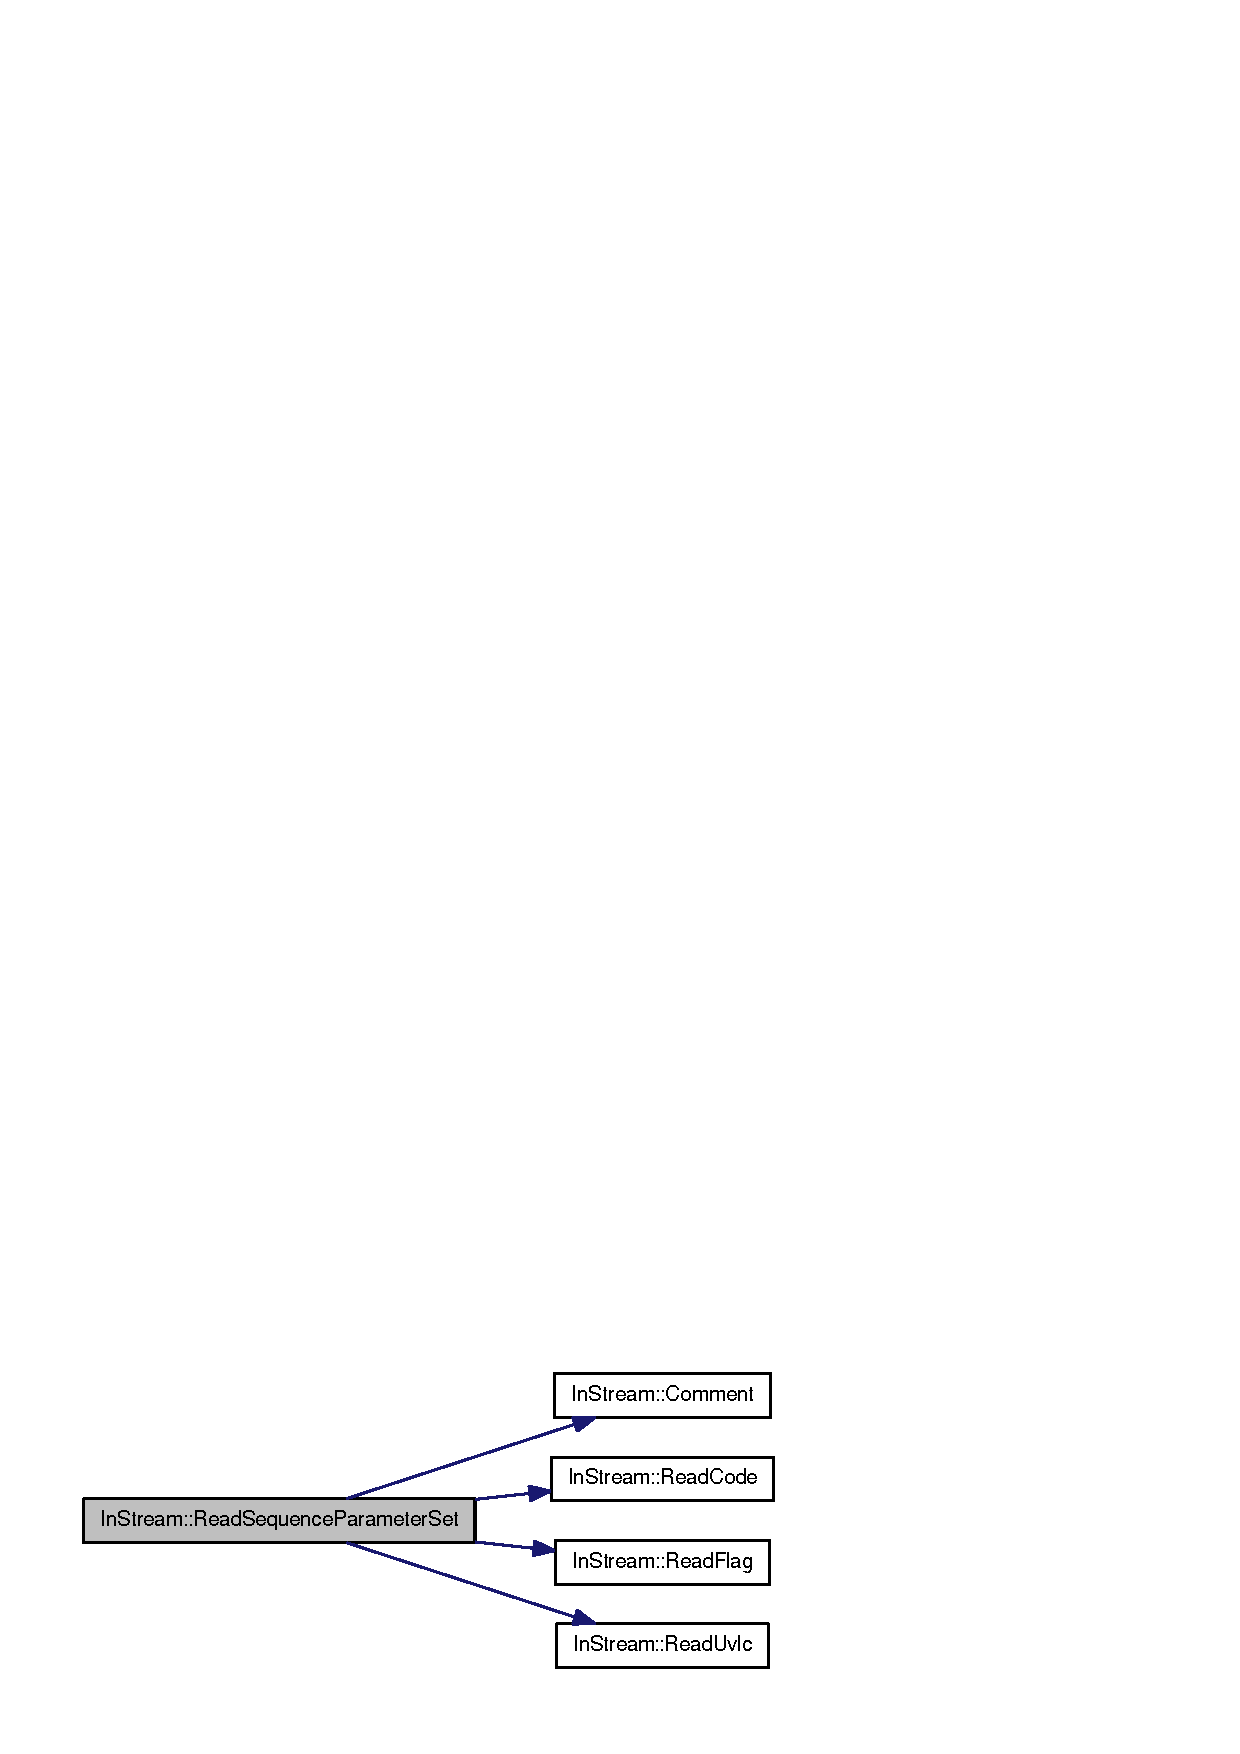
\includegraphics[width=188pt]{class_in_stream_abaa60d112267ece8de9f303623abd79d_cgraph}
\end{center}
\end{figure}


\hypertarget{class_in_stream_a6369ed63c0fad1007f16e3e885825aea}{
\index{InStream@{InStream}!ReadSliceHeader@{ReadSliceHeader}}
\index{ReadSliceHeader@{ReadSliceHeader}!InStream@{InStream}}
\subsubsection[{ReadSliceHeader}]{\setlength{\rightskip}{0pt plus 5cm}int InStream::ReadSliceHeader ({\bf SliceParameters} \& {\em sp}, \/  {\bf ArrayList}$<$ int $>$ $\ast$\& {\em ref\_\-frames}, \/  {\bf SlidingWindow} \& {\em slidingWindow}, \/  int {\em minTime})}}
\label{class_in_stream_a6369ed63c0fad1007f16e3e885825aea}




\begin{footnotesize}\begin{alltt}
00576 \{
00577         \textcolor{keywordtype}{int} long\_term\_reference\_flag = 0;
00578         \textcolor{keywordtype}{int} adaptive\_ref\_pic\_marking\_mode\_flag = 0;
00579         \textcolor{keywordtype}{int} ref\_pic\_list\_reordering\_flag0 = 0;
00580         \textcolor{keywordtype}{int} ref\_pic\_list\_reordering\_flag1 = 0;
00581         \hyperlink{struct_sequence_parameters_set}{SequenceParametersSet} &sps = \hyperlink{class_codec_info_ad439fd8062a03d868dfe9c9b615b747e}{CodecInfo::GetInstance}().\hyperlink{class_codec_info_aee785011cec77ff3c0c646b498fe1e7d}{sps};
00582         \hyperlink{struct_picture_parameters_set}{PictureParametersSet} &pps = \hyperlink{class_codec_info_ad439fd8062a03d868dfe9c9b615b747e}{CodecInfo::GetInstance}().\hyperlink{class_codec_info_abaa8d84a7d4045129ee64d91eaac4481}{pps};
00583         \textcolor{keywordtype}{int} num\_ref\_idx\_l0\_active = pps.\hyperlink{struct_picture_parameters_set_abc9eb8dcb637bef8a76a7c12380fccf9}{num_ref_idx_l0_active};
00584         \textcolor{keywordtype}{int} num\_ref\_idx\_l1\_active = pps.\hyperlink{struct_picture_parameters_set_afb1dc1e024b6c9263e33d3f1dd233203}{num_ref_idx_l1_active};
00585 
00586         \hyperlink{class_in_stream_acab96485c6978e95e5ef747ebedf09d6}{Comment}(\textcolor{stringliteral}{"NALU HEADER: forbidden\_zero\_bit"});
00587         \hyperlink{_debug_8h_a101586fab2b90a8adffe50a3550e235d}{ASSERT}(\hyperlink{class_in_stream_a340f8fadf6dfc7d17236b15285bba96f}{ReadFlag}() == 0);
00588         \hyperlink{class_in_stream_acab96485c6978e95e5ef747ebedf09d6}{Comment}(\textcolor{stringliteral}{"NALU HEADER: nal\_ref\_idc"});
00589         \textcolor{keywordtype}{int} nal\_ref\_idc = \hyperlink{class_in_stream_a07d84696f5dd53b6bbc881dc7507de4c}{ReadCode}(2);
00590         sp.\hyperlink{struct_slice_parameters_a7e551828136a39ab347f77457aa11dbb}{isRef} = (nal\_ref\_idc != 0);
00591         \hyperlink{class_in_stream_acab96485c6978e95e5ef747ebedf09d6}{Comment}(\textcolor{stringliteral}{"NALU HEADER: nal\_unit\_type"});
00592         \textcolor{keywordtype}{int} nal\_unit\_type = \hyperlink{class_in_stream_a07d84696f5dd53b6bbc881dc7507de4c}{ReadCode}(5);
00593         \textcolor{keywordflow}{if} (nal\_unit\_type==20)
00594         \{
00595                 \hyperlink{class_in_stream_acab96485c6978e95e5ef747ebedf09d6}{Comment}(\textcolor{stringliteral}{"NALU HEADER: svc\_mvc\_flag"});
00596                 \hyperlink{_debug_8h_a101586fab2b90a8adffe50a3550e235d}{ASSERT}(\hyperlink{class_in_stream_a340f8fadf6dfc7d17236b15285bba96f}{ReadFlag}() == 0);
00597                 \hyperlink{class_in_stream_acab96485c6978e95e5ef747ebedf09d6}{Comment}(\textcolor{stringliteral}{"NALU HEADER: non\_idr\_flag"});
00598                 sp.\hyperlink{struct_slice_parameters_a60f8fe21acd611ec6892e47a2c6029e3}{IDR} = (\hyperlink{class_in_stream_a340f8fadf6dfc7d17236b15285bba96f}{ReadFlag}()==0);
00599                 \hyperlink{class_in_stream_acab96485c6978e95e5ef747ebedf09d6}{Comment}(\textcolor{stringliteral}{"NALU HEADER: priority\_id"});
00600                 sp.\hyperlink{struct_slice_parameters_a82aa216a74ffaa7d1859aa1cfe135a8b}{priority_id} = \hyperlink{class_in_stream_a07d84696f5dd53b6bbc881dc7507de4c}{ReadCode}(6);
00601                 \hyperlink{class_in_stream_acab96485c6978e95e5ef747ebedf09d6}{Comment}(\textcolor{stringliteral}{"NALU HEADER: view\_id"});
00602                 sp.\hyperlink{struct_slice_parameters_ae570f1ba10b1e091c7519264534a7143}{viewId} = \hyperlink{class_in_stream_a07d84696f5dd53b6bbc881dc7507de4c}{ReadCode}(10);
00603                 \hyperlink{class_in_stream_acab96485c6978e95e5ef747ebedf09d6}{Comment}(\textcolor{stringliteral}{"NALU HEADER: temporal\_id"});
00604                 \textcolor{keywordtype}{int} temporal\_id = \hyperlink{class_in_stream_a07d84696f5dd53b6bbc881dc7507de4c}{ReadCode}(3);
00605 \textcolor{comment}{//              printf("\(\backslash\)t\(\backslash\)tTemporal Level = %d\(\backslash\)n", temporal\_id);}
00606                 \hyperlink{class_in_stream_acab96485c6978e95e5ef747ebedf09d6}{Comment}(\textcolor{stringliteral}{"NALU HEADER: anchor\_pic\_flag"});
00607                 sp.\hyperlink{struct_slice_parameters_af8a7ea94e92b177c38277af8b827eb62}{isAnchor} = (\hyperlink{class_in_stream_a07d84696f5dd53b6bbc881dc7507de4c}{ReadCode}(1) == 1);
00608                 \hyperlink{class_in_stream_acab96485c6978e95e5ef747ebedf09d6}{Comment}(\textcolor{stringliteral}{"NALU HEADER: inter\_view\_flag"});
00609                 \textcolor{keywordtype}{int} inter\_view\_flag = \hyperlink{class_in_stream_a07d84696f5dd53b6bbc881dc7507de4c}{ReadCode}(1);
00610 \textcolor{comment}{//              printf("\(\backslash\)t\(\backslash\)tInter view flag = %d\(\backslash\)n", inter\_view\_flag);}
00611                 \hyperlink{class_in_stream_acab96485c6978e95e5ef747ebedf09d6}{Comment}(\textcolor{stringliteral}{"NALU HEADER: reserved\_zero\_one\_bit"});
00612                 \hyperlink{class_in_stream_a07d84696f5dd53b6bbc881dc7507de4c}{ReadCode}(1);
00613         \}
00614         \hyperlink{class_in_stream_acab96485c6978e95e5ef747ebedf09d6}{Comment}(\textcolor{stringliteral}{"SH: first\_mb\_in\_slice"});
00615         \hyperlink{_debug_8h_a101586fab2b90a8adffe50a3550e235d}{ASSERT}(\hyperlink{class_in_stream_a8e8daf92cb96e583662cafdaf211093c}{ReadUvlc}() == 0);
00616         \hyperlink{class_in_stream_acab96485c6978e95e5ef747ebedf09d6}{Comment}(\textcolor{stringliteral}{"SH: slice\_type"});
00617         sp.\hyperlink{struct_slice_parameters_a8ab83c948c5e095477d918c0664fce0a}{SliceType} = \hyperlink{class_in_stream_a8e8daf92cb96e583662cafdaf211093c}{ReadUvlc}();
00618         \textcolor{keywordflow}{if} (sp.\hyperlink{struct_slice_parameters_a8ab83c948c5e095477d918c0664fce0a}{SliceType}>=5)
00619                 sp.\hyperlink{struct_slice_parameters_a8ab83c948c5e095477d918c0664fce0a}{SliceType} -= 5;
00620         \hyperlink{class_in_stream_acab96485c6978e95e5ef747ebedf09d6}{Comment}(\textcolor{stringliteral}{"SH: pic\_parameter\_set\_id"});
00621         \hyperlink{class_in_stream_a8e8daf92cb96e583662cafdaf211093c}{ReadUvlc}();
00622         \hyperlink{class_in_stream_acab96485c6978e95e5ef747ebedf09d6}{Comment}(\textcolor{stringliteral}{"SH: frame\_num"});
00623         sp.\hyperlink{struct_slice_parameters_a20319af06c76e833936a009f3c38d4ef}{frameNum} = \hyperlink{class_in_stream_a07d84696f5dd53b6bbc881dc7507de4c}{ReadCode}(sps.\hyperlink{struct_sequence_parameters_set_ac5f0d82a961acfe4f966e7c35aa37339}{log2nFrames});
00624 
00625         \textcolor{keywordflow}{if}( sp.\hyperlink{struct_slice_parameters_a60f8fe21acd611ec6892e47a2c6029e3}{IDR} || nal\_unit\_type==\hyperlink{_consts4_standard_8h_a0ae628337fb17a2b11855dd3524f3d04aa641b2e28c7c244e45e28f99dfc63a54}{NAL_UNIT_CODED_SLICE_IDR} )
00626         \{
00627                 \hyperlink{class_in_stream_acab96485c6978e95e5ef747ebedf09d6}{Comment}(\textcolor{stringliteral}{"SH: idr\_pic\_id"});
00628                 \textcolor{keywordtype}{int} idrPicId = \hyperlink{class_in_stream_a8e8daf92cb96e583662cafdaf211093c}{ReadUvlc}();
00629                 \textcolor{comment}{//printf("\(\backslash\)tIDR Picture ID = %d\(\backslash\)n", idrPicId);}
00630         \}
00631         \hyperlink{class_in_stream_acab96485c6978e95e5ef747ebedf09d6}{Comment}(\textcolor{stringliteral}{"SH: pic\_order\_cnt\_lsb"});
00632         sp.\hyperlink{struct_slice_parameters_ad6a26fe2f228235e4f0c31c336cf5e12}{timeId} = \hyperlink{class_in_stream_a07d84696f5dd53b6bbc881dc7507de4c}{ReadCode}(sps.\hyperlink{struct_sequence_parameters_set_aff653fc637f7290b7edbaf1cfeacd6ca}{log2nPoc});
00633         \textcolor{comment}{//sp.timeId /= 2;}
00634         \textcolor{keywordflow}{if} (sp.\hyperlink{struct_slice_parameters_ad6a26fe2f228235e4f0c31c336cf5e12}{timeId} < minTime)
00635         \{
00636                 sp.\hyperlink{struct_slice_parameters_ad6a26fe2f228235e4f0c31c336cf5e12}{timeId} |= minTime & ~sps.\hyperlink{struct_sequence_parameters_set_a786d1401a47490d15c7f1512e21994ce}{nPocM1};
00637                 \textcolor{keywordflow}{if} (sp.\hyperlink{struct_slice_parameters_ad6a26fe2f228235e4f0c31c336cf5e12}{timeId} < minTime)
00638                         sp.\hyperlink{struct_slice_parameters_ad6a26fe2f228235e4f0c31c336cf5e12}{timeId} += (1<<sps.\hyperlink{struct_sequence_parameters_set_aff653fc637f7290b7edbaf1cfeacd6ca}{log2nPoc});
00639         \}
00640         \textcolor{comment}{//printf(" TIME,VIEW = %d, %d\(\backslash\)n", sp.timeId, sp.viewId);}
00641         \textcolor{comment}{//if (sp.timeId==1 && sp.viewId==1)}
00642         \textcolor{comment}{//\{}
00643         \textcolor{comment}{//      printf("");}
00644         \textcolor{comment}{//\}}
00645         \textcolor{keywordflow}{if} (pps.\hyperlink{struct_picture_parameters_set_a9611d788502cf2646a1fafd8f1cc7e4f}{pic_order_present_flag})
00646         \{
00647                 \hyperlink{class_in_stream_acab96485c6978e95e5ef747ebedf09d6}{Comment}(\textcolor{stringliteral}{"SH: delta\_pic\_order\_cnt\_bottom"});
00648                 \hyperlink{_debug_8h_a101586fab2b90a8adffe50a3550e235d}{ASSERT}(\hyperlink{class_in_stream_accc880522e6e43bd3a46297988de1c47}{ReadSvlc}() == 0);
00649         \}
00650         \hyperlink{class_array_list}{ArrayList<Pair<int, int>} > reo0, reo1;
00651         \textcolor{keywordflow}{if} (sp.\hyperlink{struct_slice_parameters_a8ab83c948c5e095477d918c0664fce0a}{SliceType}==1 || sp.\hyperlink{struct_slice_parameters_a8ab83c948c5e095477d918c0664fce0a}{SliceType}==6) \textcolor{comment}{// B, EB}
00652         \{
00653                 \hyperlink{class_in_stream_acab96485c6978e95e5ef747ebedf09d6}{Comment}(\textcolor{stringliteral}{"SH: direct\_spatial\_mv\_pred\_flag"});
00654                 \textcolor{keywordtype}{int} direct\_spatial\_mv\_pred\_flag = \hyperlink{class_in_stream_a340f8fadf6dfc7d17236b15285bba96f}{ReadFlag}();
00655                 \hyperlink{_debug_8h_a101586fab2b90a8adffe50a3550e235d}{ASSERT}(direct\_spatial\_mv\_pred\_flag == 1)
00656         \}
00657         \textcolor{keywordflow}{if} (sp.\hyperlink{struct_slice_parameters_a8ab83c948c5e095477d918c0664fce0a}{SliceType}==0 || sp.\hyperlink{struct_slice_parameters_a8ab83c948c5e095477d918c0664fce0a}{SliceType}==1 || sp.\hyperlink{struct_slice_parameters_a8ab83c948c5e095477d918c0664fce0a}{SliceType}==5 || sp.
      \hyperlink{struct_slice_parameters_a8ab83c948c5e095477d918c0664fce0a}{SliceType}==6)
00658         \{
00659                 \hyperlink{class_in_stream_acab96485c6978e95e5ef747ebedf09d6}{Comment}(\textcolor{stringliteral}{"SH: num\_ref\_idx\_active\_override\_flag"});
00660                 \textcolor{keywordtype}{int} num\_ref\_idx\_active\_override\_flag = \hyperlink{class_in_stream_a340f8fadf6dfc7d17236b15285bba96f}{ReadFlag}();
00661                 \textcolor{keywordflow}{if} (num\_ref\_idx\_active\_override\_flag)
00662                 \{
00663                         \hyperlink{class_in_stream_acab96485c6978e95e5ef747ebedf09d6}{Comment}(\textcolor{stringliteral}{"SH: num\_ref\_idx\_l0\_active\_minus1"});
00664                         num\_ref\_idx\_l0\_active = \hyperlink{class_in_stream_a8e8daf92cb96e583662cafdaf211093c}{ReadUvlc}() + 1;
00665                         \textcolor{keywordflow}{if} (sp.\hyperlink{struct_slice_parameters_a8ab83c948c5e095477d918c0664fce0a}{SliceType}==1 || sp.\hyperlink{struct_slice_parameters_a8ab83c948c5e095477d918c0664fce0a}{SliceType}==6)
00666                         \{
00667                                 \hyperlink{class_in_stream_acab96485c6978e95e5ef747ebedf09d6}{Comment}(\textcolor{stringliteral}{"SH: num\_ref\_idx\_l1\_active\_minus1"});
00668                                 num\_ref\_idx\_l1\_active = \hyperlink{class_in_stream_a8e8daf92cb96e583662cafdaf211093c}{ReadUvlc}() + 1;
00669                         \}
00670                 \}
00671                 \hyperlink{class_in_stream_acab96485c6978e95e5ef747ebedf09d6}{Comment}(\textcolor{stringliteral}{"RIR: ref\_pic\_list\_reordering\_flag"});
00672                 ref\_pic\_list\_reordering\_flag0 = \hyperlink{class_in_stream_a340f8fadf6dfc7d17236b15285bba96f}{ReadFlag}();
00673                 \textcolor{keywordflow}{if} (ref\_pic\_list\_reordering\_flag0)
00674                 \{
00675                         \textcolor{keywordtype}{int} reordering\_of\_pic\_nums\_idc;
00676                         \textcolor{keywordtype}{int} tt = 10;
00677                         \textcolor{keywordflow}{do} \{
00678                                 reordering\_of\_pic\_nums\_idc = \hyperlink{class_in_stream_a8e8daf92cb96e583662cafdaf211093c}{ReadUvlc}();
00679                                 \textcolor{keywordtype}{int} va = 0;
00680                                 \textcolor{keywordflow}{if} (reordering\_of\_pic\_nums\_idc != 3)
00681                                         va = \hyperlink{class_in_stream_a8e8daf92cb96e583662cafdaf211093c}{ReadUvlc}();
00682                                 reo0.\hyperlink{class_array_list_a7b5376678a9b5af0e0ed913fbe04b902}{push_back}(\hyperlink{_pair_8h_a76ecd40e2cff7790abf204644d74645e}{makePair}(reordering\_of\_pic\_nums\_id
      c, va+1));
00683                                 \hyperlink{_debug_8h_a101586fab2b90a8adffe50a3550e235d}{ASSERT}(tt--);
00684                         \} \textcolor{keywordflow}{while} (reordering\_of\_pic\_nums\_idc != 3);
00685                 \}
00686                 \textcolor{keywordflow}{if} (sp.\hyperlink{struct_slice_parameters_a8ab83c948c5e095477d918c0664fce0a}{SliceType}==1 || sp.\hyperlink{struct_slice_parameters_a8ab83c948c5e095477d918c0664fce0a}{SliceType}==6) \textcolor{comment}{// B, EB}
00687                 \{
00688                         \hyperlink{class_in_stream_acab96485c6978e95e5ef747ebedf09d6}{Comment}(\textcolor{stringliteral}{"RIR: ref\_pic\_list\_reordering\_flag"});
00689                         ref\_pic\_list\_reordering\_flag1 = \hyperlink{class_in_stream_a340f8fadf6dfc7d17236b15285bba96f}{ReadFlag}();
00690                         \textcolor{keywordtype}{int} tt = 5;
00691                         \textcolor{keywordflow}{if} (ref\_pic\_list\_reordering\_flag1)
00692                         \{
00693                                 \textcolor{keywordtype}{int} reordering\_of\_pic\_nums\_idc;
00694                                 \textcolor{keywordflow}{do} \{
00695                                         reordering\_of\_pic\_nums\_idc = \hyperlink{class_in_stream_a8e8daf92cb96e583662cafdaf211093c}{ReadUvlc}();
00696                                         \textcolor{keywordtype}{int} va = 0;
00697                                         \textcolor{keywordflow}{if} (reordering\_of\_pic\_nums\_idc != 3)
00698                                                 va = \hyperlink{class_in_stream_a8e8daf92cb96e583662cafdaf211093c}{ReadUvlc}();
00699                                         reo1.\hyperlink{class_array_list_a7b5376678a9b5af0e0ed913fbe04b902}{push_back}(\hyperlink{_pair_8h_a76ecd40e2cff7790abf204644d74645e}{makePair}(reordering\_of\_pic
      \_nums\_idc, va+1));
00700                                         \hyperlink{_debug_8h_a101586fab2b90a8adffe50a3550e235d}{ASSERT}(tt--);
00701                                 \} \textcolor{keywordflow}{while} (reordering\_of\_pic\_nums\_idc != 3);
00702                         \}
00703                 \}
00704         \}
00705 
00706         \textcolor{keywordflow}{if} (nal\_ref\_idc)
00707         \{
00708                 \textcolor{keywordflow}{if} (nal\_unit\_type==5 || sp.\hyperlink{struct_slice_parameters_a60f8fe21acd611ec6892e47a2c6029e3}{IDR})
00709                 \{
00710                         \hyperlink{class_in_stream_acab96485c6978e95e5ef747ebedf09d6}{Comment}(\textcolor{stringliteral}{"DRPM: no\_output\_of\_prior\_pics\_flag"});
00711                         \textcolor{keywordtype}{int} no\_output\_of\_prior\_pics\_flag = \hyperlink{class_in_stream_a340f8fadf6dfc7d17236b15285bba96f}{ReadFlag}();
00712                         \textcolor{comment}{//printf("\(\backslash\)t\(\backslash\)tno\_output\_of\_prior\_pics\_flag = %d\(\backslash\)n", no\_ou
      tput\_of\_prior\_pics\_flag);}
00713                         \hyperlink{class_in_stream_acab96485c6978e95e5ef747ebedf09d6}{Comment}(\textcolor{stringliteral}{"DRPM: long\_term\_reference\_flag"});
00714                         long\_term\_reference\_flag = \hyperlink{class_in_stream_a340f8fadf6dfc7d17236b15285bba96f}{ReadFlag}();
00715                         \textcolor{comment}{//printf("\(\backslash\)t\(\backslash\)tlong\_term\_reference\_flag = %d\(\backslash\)n", long\_term
      \_reference\_flag);}
00716                 \}
00717                 \textcolor{keywordflow}{else}
00718                 \{
00719                         \hyperlink{class_in_stream_acab96485c6978e95e5ef747ebedf09d6}{Comment}(\textcolor{stringliteral}{"adaptive\_ref\_pic\_marking\_mode\_flag"});
00720                         adaptive\_ref\_pic\_marking\_mode\_flag = \hyperlink{class_in_stream_a340f8fadf6dfc7d17236b15285bba96f}{ReadFlag}();
00721                         \textcolor{keywordflow}{if} (adaptive\_ref\_pic\_marking\_mode\_flag)
00722                         \{
00723                                 \textcolor{keywordtype}{int} memory\_management\_control\_operation;
00724                                 \textcolor{keywordtype}{int} pb, pa;
00725                                 \textcolor{keywordflow}{do} \{
00726                                         memory\_management\_control\_operation = 
      \hyperlink{class_in_stream_a8e8daf92cb96e583662cafdaf211093c}{ReadUvlc}();
00727                                         pa = pb = 0;
00728                                         \textcolor{keywordflow}{switch} (memory\_management\_control\_operati
      on)
00729                                         \{
00730                                         \textcolor{keywordflow}{case} 3:
00731                                                 pb = \hyperlink{class_in_stream_a8e8daf92cb96e583662cafdaf211093c}{ReadUvlc}();
00732 
00733                                         \textcolor{keywordflow}{case} 1:
00734                                         \textcolor{keywordflow}{case} 2:
00735                                         \textcolor{keywordflow}{case} 4:
00736                                         \textcolor{keywordflow}{case} 6:
00737                                                 pa = \hyperlink{class_in_stream_a8e8daf92cb96e583662cafdaf211093c}{ReadUvlc}();
00738 
00739                                         \textcolor{keywordflow}{case} 5:
00740                                         \textcolor{keywordflow}{default} : 
00741                                                 ;
00742                                         \}
00743                                         \textcolor{keywordflow}{if} (memory\_management\_control\_operation==
      0)
00744                                         \{
00745 
00746                                         \}
00747                                         \textcolor{keywordflow}{else} \textcolor{keywordflow}{if} (memory\_management\_control\_operat
      ion==1)
00748                                         \{
00749                                                 \textcolor{keywordtype}{int} fn = sp.\hyperlink{struct_slice_parameters_a20319af06c76e833936a009f3c38d4ef}{frameNum} - pa - 1;
00750                                                 \textcolor{keywordtype}{bool} find = \textcolor{keyword}{false};
00751                                                 \textcolor{keywordflow}{for} (\textcolor{keywordtype}{int} x = 0; x < ref\_frames[sp
      .\hyperlink{struct_slice_parameters_ae570f1ba10b1e091c7519264534a7143}{viewId}].\hyperlink{class_array_list_aff9c6ac40886044e4653174950d23e74}{size}(); ++x)
00752                                                         \textcolor{keywordflow}{if} (slidingWindow.
      \hyperlink{class_sliding_window_a020d2c25f1bda31337f91bf9b1a809d1}{GetSliceParameters}(ref\_frames[sp.\hyperlink{struct_slice_parameters_ae570f1ba10b1e091c7519264534a7143}{viewId}][x], sp.\hyperlink{struct_slice_parameters_ae570f1ba10b1e091c7519264534a7143}{viewId})->\hyperlink{struct_slice_parameters_a20319af06c76e833936a009f3c38d4ef}{frameNum} == fn)
00753                                                         \{
00754                                                                 ref\_frames[sp.
      \hyperlink{struct_slice_parameters_ae570f1ba10b1e091c7519264534a7143}{viewId}].\hyperlink{class_array_list_a18695cf2c26e9c6ef585ec77afc19fc6}{erase}(x);
00755                                                                 find = \textcolor{keyword}{true};
00756                                                                 \textcolor{keywordflow}{break};
00757                                                         \}
00758                                                         \textcolor{keywordflow}{if} (!find)
00759                                                         \{
00760                                                                 \hyperlink{_debug_8h_a101586fab2b90a8adffe50a3550e235d}{ASSERT}(0);
00761                                                         \}
00762                                         \}
00763                                         \textcolor{keywordflow}{else}
00764                                         \{
00765                                                 \hyperlink{_debug_8h_a101586fab2b90a8adffe50a3550e235d}{ASSERT}(0);
00766                                         \}
00767 
00768                                 \} \textcolor{keywordflow}{while} (memory\_management\_control\_operation != 0
      );
00769                         \}
00770                 \}
00771         \}
00772 
00773         \hyperlink{class_in_stream_acab96485c6978e95e5ef747ebedf09d6}{Comment}(\textcolor{stringliteral}{"SH: slice\_qp\_delta"});
00774         sp.\hyperlink{struct_slice_parameters_a5ca0d343251519b63746af21c1cb9f70}{QP_Delta} = \hyperlink{class_in_stream_accc880522e6e43bd3a46297988de1c47}{ReadSvlc}();
00775 
00776         \hyperlink{class_array_list}{ArrayList<Pair<int, int>} > list0, list1;
00777         \textcolor{keywordflow}{if} (sp.\hyperlink{struct_slice_parameters_a8ab83c948c5e095477d918c0664fce0a}{SliceType} == 2)
00778         \{
00779                 ; \textcolor{comment}{// Nothing}
00780         \}
00781         \textcolor{keywordflow}{else} \textcolor{keywordflow}{if} (sp.\hyperlink{struct_slice_parameters_a8ab83c948c5e095477d918c0664fce0a}{SliceType} == 1)
00782         \{
00783                 \textcolor{keywordflow}{for} (\textcolor{keywordtype}{int} i = 0; i < ref\_frames[sp.\hyperlink{struct_slice_parameters_ae570f1ba10b1e091c7519264534a7143}{viewId}].\hyperlink{class_array_list_aff9c6ac40886044e4653174950d23e74}{size}(); ++i)
00784                         list0.\hyperlink{class_array_list_a7b5376678a9b5af0e0ed913fbe04b902}{push_back}(\hyperlink{_pair_8h_a76ecd40e2cff7790abf204644d74645e}{makePair}(ref\_frames[sp.\hyperlink{struct_slice_parameters_ae570f1ba10b1e091c7519264534a7143}{viewId}][i], sp.
      \hyperlink{struct_slice_parameters_ae570f1ba10b1e091c7519264534a7143}{viewId}));
00785                 list1 = list0;
00786                 \textcolor{keywordflow}{for} (\textcolor{keywordtype}{int} i = list0.\hyperlink{class_array_list_aff9c6ac40886044e4653174950d23e74}{size}() - 1; i >= 0; --i)
00787                 \{
00788                         \textcolor{keywordflow}{for} (\textcolor{keywordtype}{int} j = 0; j < i; ++j)
00789                                 \textcolor{keywordflow}{if} (list0[j].first>=sp.\hyperlink{struct_slice_parameters_ad6a26fe2f228235e4f0c31c336cf5e12}{timeId} && list0[j+1].first
      <sp.\hyperlink{struct_slice_parameters_ad6a26fe2f228235e4f0c31c336cf5e12}{timeId} ||
00790                                         list0[j+1].first<sp.\hyperlink{struct_slice_parameters_ad6a26fe2f228235e4f0c31c336cf5e12}{timeId} && list0[j+1].
      first>list0[j].first ||
00791                                         list0[j+1].first>=sp.\hyperlink{struct_slice_parameters_ad6a26fe2f228235e4f0c31c336cf5e12}{timeId} && list0[j+1]
      .first<list0[j].first)
00792                                 \{
00793                                         \hyperlink{class_pair}{Pair<int, int>} tmp = list0[j]; list0[j] =
       list0[j+1]; list0[j+1] = tmp;
00794                                 \}
00795                 \}
00796                 \textcolor{keywordflow}{for} (\textcolor{keywordtype}{int} i = list0.\hyperlink{class_array_list_aff9c6ac40886044e4653174950d23e74}{size}() - 1; i >= 0; --i)
00797                 \{
00798                         \textcolor{keywordflow}{for} (\textcolor{keywordtype}{int} j = 0; j < i; ++j)
00799                                 \textcolor{keywordflow}{if} (list1[j].first<=sp.\hyperlink{struct_slice_parameters_ad6a26fe2f228235e4f0c31c336cf5e12}{timeId} && list1[j+1].first
      >sp.\hyperlink{struct_slice_parameters_ad6a26fe2f228235e4f0c31c336cf5e12}{timeId} ||
00800                                         list1[j+1].first<=sp.\hyperlink{struct_slice_parameters_ad6a26fe2f228235e4f0c31c336cf5e12}{timeId} && list1[j+1]
      .first>list1[j].first ||
00801                                         list1[j+1].first>sp.\hyperlink{struct_slice_parameters_ad6a26fe2f228235e4f0c31c336cf5e12}{timeId} && list1[j+1].
      first<list1[j].first)
00802                                 \{
00803                                         \hyperlink{class_pair}{Pair<int, int>} tmp = list1[j]; list1[j] =
       list1[j+1]; list1[j+1] = tmp;
00804                                 \}
00805                 \}
00806         \}
00807         \textcolor{keywordflow}{else} \textcolor{keywordflow}{if} (sp.\hyperlink{struct_slice_parameters_a8ab83c948c5e095477d918c0664fce0a}{SliceType} == 0)
00808         \{
00809                 \textcolor{keywordflow}{for} (\textcolor{keywordtype}{int} i = 0; i < ref\_frames[sp.\hyperlink{struct_slice_parameters_ae570f1ba10b1e091c7519264534a7143}{viewId}].\hyperlink{class_array_list_aff9c6ac40886044e4653174950d23e74}{size}(); ++i)
00810                         list0.\hyperlink{class_array_list_a7b5376678a9b5af0e0ed913fbe04b902}{push_back}(\hyperlink{_pair_8h_a76ecd40e2cff7790abf204644d74645e}{makePair}(ref\_frames[sp.\hyperlink{struct_slice_parameters_ae570f1ba10b1e091c7519264534a7143}{viewId}][i], sp.
      \hyperlink{struct_slice_parameters_ae570f1ba10b1e091c7519264534a7143}{viewId}));
00811                 \textcolor{keywordflow}{for} (\textcolor{keywordtype}{int} i = list0.\hyperlink{class_array_list_aff9c6ac40886044e4653174950d23e74}{size}() - 1; i >= 0; --i)
00812                         \textcolor{keywordflow}{for} (\textcolor{keywordtype}{int} j = 0; j < i; ++j)
00813                         \{
00814                                 \textcolor{keywordflow}{if} (slidingWindow.\hyperlink{class_sliding_window_a020d2c25f1bda31337f91bf9b1a809d1}{GetSliceParameters}(list0[j].fir
      st, list0[j].second)->\hyperlink{struct_slice_parameters_a20319af06c76e833936a009f3c38d4ef}{frameNum} <
00815                                         slidingWindow.\hyperlink{class_sliding_window_a020d2c25f1bda31337f91bf9b1a809d1}{GetSliceParameters}(list0[j+
      1].first, list0[j+1].second)->\hyperlink{struct_slice_parameters_a20319af06c76e833936a009f3c38d4ef}{frameNum})
00816                                 \{
00817                                         \hyperlink{class_pair}{Pair<int, int>} tmp = list0[j]; list0[j] =
       list0[j+1]; list0[j+1] = tmp;
00818                                 \}
00819                         \}
00820         \}
00821         \textcolor{keywordflow}{else}
00822         \{
00823                 \hyperlink{_debug_8h_a101586fab2b90a8adffe50a3550e235d}{ASSERT}(0);
00824         \}
00825 
00826 
00827 
00828         \textcolor{keywordflow}{if} (sp.\hyperlink{struct_slice_parameters_af8a7ea94e92b177c38277af8b827eb62}{isAnchor})
00829         \{
00830                 \textcolor{keywordflow}{for} (\textcolor{keywordtype}{int} i = 0; i < sps.\hyperlink{struct_sequence_parameters_set_ae9b6a7d85da9fec255cca59c3d750ecd}{anchorRefsList0}[sp.\hyperlink{struct_slice_parameters_ae570f1ba10b1e091c7519264534a7143}{viewId}].\hyperlink{class_array_list_aff9c6ac40886044e4653174950d23e74}{size}(); ++i)
00831                         list0.\hyperlink{class_array_list_a7b5376678a9b5af0e0ed913fbe04b902}{push_back}(\hyperlink{_pair_8h_a76ecd40e2cff7790abf204644d74645e}{makePair}(sp.\hyperlink{struct_slice_parameters_ad6a26fe2f228235e4f0c31c336cf5e12}{timeId}, sps.\hyperlink{struct_sequence_parameters_set_ae9b6a7d85da9fec255cca59c3d750ecd}{anchorRefsList0}[s
      p.\hyperlink{struct_slice_parameters_ae570f1ba10b1e091c7519264534a7143}{viewId}][i]));
00832                 \textcolor{keywordflow}{for} (\textcolor{keywordtype}{int} i = 0; i < sps.\hyperlink{struct_sequence_parameters_set_a7b865f89c34428785081c3c4acadc965}{anchorRefsList1}[sp.\hyperlink{struct_slice_parameters_ae570f1ba10b1e091c7519264534a7143}{viewId}].\hyperlink{class_array_list_aff9c6ac40886044e4653174950d23e74}{size}(); ++i)
00833                         list1.\hyperlink{class_array_list_a7b5376678a9b5af0e0ed913fbe04b902}{push_back}(\hyperlink{_pair_8h_a76ecd40e2cff7790abf204644d74645e}{makePair}(sp.\hyperlink{struct_slice_parameters_ad6a26fe2f228235e4f0c31c336cf5e12}{timeId}, sps.\hyperlink{struct_sequence_parameters_set_a7b865f89c34428785081c3c4acadc965}{anchorRefsList1}[s
      p.\hyperlink{struct_slice_parameters_ae570f1ba10b1e091c7519264534a7143}{viewId}][i]));
00834         \}
00835         \textcolor{keywordflow}{else}
00836         \{
00837                 \textcolor{keywordflow}{for} (\textcolor{keywordtype}{int} i = 0; i < sps.\hyperlink{struct_sequence_parameters_set_ab9b078b23e746ef60f7697896b963b93}{nonAnchorRefsList0}[sp.\hyperlink{struct_slice_parameters_ae570f1ba10b1e091c7519264534a7143}{viewId}].\hyperlink{class_array_list_aff9c6ac40886044e4653174950d23e74}{size}(); ++i
      )
00838                         list0.\hyperlink{class_array_list_a7b5376678a9b5af0e0ed913fbe04b902}{push_back}(\hyperlink{_pair_8h_a76ecd40e2cff7790abf204644d74645e}{makePair}(sp.\hyperlink{struct_slice_parameters_ad6a26fe2f228235e4f0c31c336cf5e12}{timeId}, sps.
      \hyperlink{struct_sequence_parameters_set_ab9b078b23e746ef60f7697896b963b93}{nonAnchorRefsList0}[sp.\hyperlink{struct_slice_parameters_ae570f1ba10b1e091c7519264534a7143}{viewId}][i]));
00839                 \textcolor{keywordflow}{for} (\textcolor{keywordtype}{int} i = 0; i < sps.\hyperlink{struct_sequence_parameters_set_a68b7ffb23b151c53312798f7ab79a67a}{nonAnchorRefsList1}[sp.\hyperlink{struct_slice_parameters_ae570f1ba10b1e091c7519264534a7143}{viewId}].\hyperlink{class_array_list_aff9c6ac40886044e4653174950d23e74}{size}(); ++i
      )
00840                         list1.\hyperlink{class_array_list_a7b5376678a9b5af0e0ed913fbe04b902}{push_back}(\hyperlink{_pair_8h_a76ecd40e2cff7790abf204644d74645e}{makePair}(sp.\hyperlink{struct_slice_parameters_ad6a26fe2f228235e4f0c31c336cf5e12}{timeId}, sps.
      \hyperlink{struct_sequence_parameters_set_a68b7ffb23b151c53312798f7ab79a67a}{nonAnchorRefsList1}[sp.\hyperlink{struct_slice_parameters_ae570f1ba10b1e091c7519264534a7143}{viewId}][i]));
00841         \}
00842 
00843 \textcolor{preprocessor}{#define RPLR\_NEG 0}
00844 \textcolor{preprocessor}{}\textcolor{preprocessor}{#define RPLR\_POS 1}
00845 \textcolor{preprocessor}{}\textcolor{preprocessor}{#define RPLR\_LONG 2}
00846 \textcolor{preprocessor}{}\textcolor{preprocessor}{#define RPLR\_END 3}
00847 \textcolor{preprocessor}{}\textcolor{preprocessor}{#define RPLR\_VIEW\_NEG 4}
00848 \textcolor{preprocessor}{}\textcolor{preprocessor}{#define RPLR\_VIEW\_POS 5}
00849 \textcolor{preprocessor}{}
00850         \textcolor{keywordflow}{if} (ref\_pic\_list\_reordering\_flag0)
00851         \{
00852                 \textcolor{keywordtype}{int}  uiPicNumPred    = sp.\hyperlink{struct_slice_parameters_a20319af06c76e833936a009f3c38d4ef}{frameNum};
00853                 \textcolor{keywordtype}{int}  uiIndex         = 0;   
00854                 \textcolor{keywordtype}{int}  uiCommand       = 0;   
00855                 \textcolor{keywordtype}{int}  uiIdentifier    = 0;   
00856                 \textcolor{comment}{// JVT-V043   }
00857                 \hyperlink{_types_8h_a943a9a9a987cd1f4d16d71dd0ae23721}{UInt}  uiPicViewIdx    = -1;   
00858                 \textcolor{keywordflow}{for} (\textcolor{keywordtype}{int} i = 0; i < reo0.\hyperlink{class_array_list_aff9c6ac40886044e4653174950d23e74}{size}(); ++i)
00859                 \{   
00860                         uiCommand = reo0[i].first;
00861                         uiIdentifier = reo0[i].second - 1;
00862                         \textcolor{keywordflow}{if} (uiCommand == 3)
00863                                 \textcolor{keywordflow}{break};
00864                         \textcolor{keywordflow}{if}( uiCommand == RPLR\_LONG )   
00865                         \{   
00866                                 \textcolor{comment}{//===== long-term index =====   }
00867                                 \hyperlink{_debug_8h_a101586fab2b90a8adffe50a3550e235d}{ASSERT}(0);
00868                         \}   
00869                         \textcolor{keywordflow}{else} \textcolor{keywordflow}{if} (uiCommand == RPLR\_NEG || uiCommand == RPLR\_POS) 
      \textcolor{comment}{// JVT-V043    }
00870                         \{   
00871                                 \textcolor{comment}{//===== short-term index =====   }
00872                                 \textcolor{keywordtype}{int} uiAbsDiff = uiIdentifier + 1;   
00873                                 \textcolor{keywordflow}{if}( uiCommand == RPLR\_NEG )
00874                                         uiAbsDiff = -uiAbsDiff;
00875                                 uiPicNumPred += uiAbsDiff;   
00876                                 uiPicNumPred &= sps.\hyperlink{struct_sequence_parameters_set_afedac9d01de6ec718715ab45c63ee999}{nFramesM1};
00877                                 uiIdentifier = uiPicNumPred;   
00878 
00879                                 \textcolor{comment}{//----- get frame -----   }
00880                                 \textcolor{keywordtype}{int} ft = -1;
00881                                 \textcolor{keywordflow}{for} (\textcolor{keywordtype}{int} x = 0; x < ref\_frames[sp.\hyperlink{struct_slice_parameters_ae570f1ba10b1e091c7519264534a7143}{viewId}].\hyperlink{class_array_list_aff9c6ac40886044e4653174950d23e74}{size}();
       ++x)
00882                                         \textcolor{keywordflow}{if} (slidingWindow.\hyperlink{class_sliding_window_a020d2c25f1bda31337f91bf9b1a809d1}{GetSliceParameters}(ref\_
      frames[sp.\hyperlink{struct_slice_parameters_ae570f1ba10b1e091c7519264534a7143}{viewId}][x], sp.\hyperlink{struct_slice_parameters_ae570f1ba10b1e091c7519264534a7143}{viewId})->\hyperlink{struct_slice_parameters_a20319af06c76e833936a009f3c38d4ef}{frameNum} == uiIdentifier)
00883                                         \{
00884                                                 ft = ref\_frames[sp.\hyperlink{struct_slice_parameters_ae570f1ba10b1e091c7519264534a7143}{viewId}][x];
00885                                                 \textcolor{keywordflow}{break};
00886                                         \}
00887                                         \textcolor{keywordflow}{if} (ft < 0)
00888                                         \{
00889                                                 \hyperlink{_debug_8h_a101586fab2b90a8adffe50a3550e235d}{ASSERT}(0);
00890                                         \}
00891                                         \textcolor{keywordtype}{int} p = -1;
00892                                         \textcolor{keywordflow}{for} (\textcolor{keywordtype}{int} x = uiIndex; x < list0.\hyperlink{class_array_list_aff9c6ac40886044e4653174950d23e74}{size}(); +
      +x)
00893                                                 \textcolor{keywordflow}{if} (list0[x].first == ft && list0
      [x].second == sp.\hyperlink{struct_slice_parameters_ae570f1ba10b1e091c7519264534a7143}{viewId})
00894                                                 \{
00895                                                         list0.\hyperlink{class_array_list_a18695cf2c26e9c6ef585ec77afc19fc6}{erase}(x);
00896                                                         \textcolor{keywordflow}{break};
00897                                                 \}
00898                                                 list0.\hyperlink{class_array_list_addb12a5554260fa1f386160ce8534db0}{insert}(uiIndex, \hyperlink{_pair_8h_a76ecd40e2cff7790abf204644d74645e}{makePair}(ft
      , sp.\hyperlink{struct_slice_parameters_ae570f1ba10b1e091c7519264534a7143}{viewId}));
00899                                                 uiIndex++;   
00900                         \} \textcolor{comment}{// short-term   }
00901                         \textcolor{keywordflow}{else} \textcolor{comment}{// 4 or 5   }
00902                         \{   
00903                                 \hyperlink{_types_8h_a943a9a9a987cd1f4d16d71dd0ae23721}{UInt} uiAbsDiff = uiIdentifier + 1;   
00904                                 \textcolor{comment}{// JVT-W066   }
00905                                 \hyperlink{_types_8h_a943a9a9a987cd1f4d16d71dd0ae23721}{UInt} uiMaxRef;
00906                                 \textcolor{keywordflow}{if} (sp.\hyperlink{struct_slice_parameters_af8a7ea94e92b177c38277af8b827eb62}{isAnchor})
00907                                         uiMaxRef = sps.\hyperlink{struct_sequence_parameters_set_ae9b6a7d85da9fec255cca59c3d750ecd}{anchorRefsList0}[sp.\hyperlink{struct_slice_parameters_ae570f1ba10b1e091c7519264534a7143}{viewId}]
      .\hyperlink{class_array_list_aff9c6ac40886044e4653174950d23e74}{size}();
00908                                 \textcolor{keywordflow}{else}
00909                                         uiMaxRef = sps.\hyperlink{struct_sequence_parameters_set_ab9b078b23e746ef60f7697896b963b93}{nonAnchorRefsList0}[sp.
      \hyperlink{struct_slice_parameters_ae570f1ba10b1e091c7519264534a7143}{viewId}].\hyperlink{class_array_list_aff9c6ac40886044e4653174950d23e74}{size}();
00910 
00911                                 \textcolor{keywordflow}{if}( uiCommand == RPLR\_VIEW\_NEG )   
00912                                         uiAbsDiff = uiMaxRef - uiAbsDiff;
00913                                 uiPicViewIdx +=   uiAbsDiff;   
00914                                 \textcolor{keywordflow}{if}( uiPicViewIdx >= uiMaxRef )   
00915                                         uiPicViewIdx -= uiMaxRef;
00916                                 \textcolor{comment}{// JVT-W066   }
00917                                 uiIdentifier = uiPicViewIdx;    
00918 
00919 
00920                                 \textcolor{keywordtype}{int} targetViewId;
00921                                 \textcolor{keywordflow}{if} (sp.\hyperlink{struct_slice_parameters_af8a7ea94e92b177c38277af8b827eb62}{isAnchor})
00922                                         targetViewId = sps.\hyperlink{struct_sequence_parameters_set_ae9b6a7d85da9fec255cca59c3d750ecd}{anchorRefsList0}[sp.
      \hyperlink{struct_slice_parameters_ae570f1ba10b1e091c7519264534a7143}{viewId}][uiIdentifier];
00923                                 \textcolor{keywordflow}{else}
00924                                         targetViewId = sps.\hyperlink{struct_sequence_parameters_set_ab9b078b23e746ef60f7697896b963b93}{nonAnchorRefsList0}[sp.
      \hyperlink{struct_slice_parameters_ae570f1ba10b1e091c7519264534a7143}{viewId}][uiIdentifier];
00925 
00926                                 \textcolor{comment}{//----- find picture in reference list -----   }
00927                                 \textcolor{keywordflow}{for} (\textcolor{keywordtype}{int} x = 0; x < list0.\hyperlink{class_array_list_aff9c6ac40886044e4653174950d23e74}{size}(); ++x)
00928                                         \textcolor{keywordflow}{if} (list0[x].first == sp.\hyperlink{struct_slice_parameters_ad6a26fe2f228235e4f0c31c336cf5e12}{timeId} && list0[
      x].second == targetViewId)
00929                                         \{   
00930                                                 list0.\hyperlink{class_array_list_a18695cf2c26e9c6ef585ec77afc19fc6}{erase}(x);
00931                                                 \textcolor{keywordflow}{break};
00932                                         \}  
00933                                         list0.\hyperlink{class_array_list_addb12a5554260fa1f386160ce8534db0}{insert}(uiIndex, \hyperlink{_pair_8h_a76ecd40e2cff7790abf204644d74645e}{makePair}(sp.\hyperlink{struct_slice_parameters_ad6a26fe2f228235e4f0c31c336cf5e12}{timeId},
       targetViewId));
00934 
00935                                         uiIndex++;   
00936                         \} \textcolor{comment}{// inter-view    }
00937                 \} \textcolor{comment}{// while   }
00938         \}
00939         \textcolor{keywordflow}{if} (ref\_pic\_list\_reordering\_flag1)
00940         \{
00941                 \textcolor{keywordtype}{int}  uiPicNumPred    = sp.\hyperlink{struct_slice_parameters_a20319af06c76e833936a009f3c38d4ef}{frameNum};
00942                 \textcolor{keywordtype}{int}  uiIndex         = 0;   
00943                 \textcolor{keywordtype}{int}  uiCommand       = 0;   
00944                 \textcolor{keywordtype}{int}  uiIdentifier    = 0;   
00945                 \textcolor{comment}{// JVT-V043   }
00946                 \hyperlink{_types_8h_a943a9a9a987cd1f4d16d71dd0ae23721}{UInt}  uiPicViewIdx    = -1;   
00947                 \textcolor{keywordflow}{for} (\textcolor{keywordtype}{int} i = 0; i < reo1.\hyperlink{class_array_list_aff9c6ac40886044e4653174950d23e74}{size}(); ++i)
00948                 \{   
00949                         uiCommand = reo1[i].first;
00950                         uiIdentifier = reo1[i].second - 1;
00951                         \textcolor{keywordflow}{if} (uiCommand == 3)
00952                                 \textcolor{keywordflow}{break};
00953                         \textcolor{keywordflow}{if}( uiCommand == RPLR\_LONG )   
00954                         \{   
00955                                 \textcolor{comment}{//===== long-term index =====   }
00956                                 \hyperlink{_debug_8h_a101586fab2b90a8adffe50a3550e235d}{ASSERT}(0);
00957                         \}   
00958                         \textcolor{keywordflow}{else} \textcolor{keywordflow}{if} (uiCommand == RPLR\_NEG || uiCommand == RPLR\_POS) 
      \textcolor{comment}{// JVT-V043    }
00959                         \{   
00960                                 \textcolor{comment}{//===== short-term index =====   }
00961                                 \textcolor{keywordtype}{int} uiAbsDiff = uiIdentifier + 1;   
00962                                 \textcolor{keywordflow}{if}( uiCommand == RPLR\_NEG )
00963                                         uiAbsDiff = -uiAbsDiff;
00964                                 uiPicNumPred += uiAbsDiff;   
00965                                 uiPicNumPred &= sps.\hyperlink{struct_sequence_parameters_set_afedac9d01de6ec718715ab45c63ee999}{nFramesM1};
00966                                 uiIdentifier = uiPicNumPred;   
00967 
00968                                 \textcolor{comment}{//----- get frame -----   }
00969                                 \textcolor{keywordtype}{int} ft = -1;
00970                                 \textcolor{keywordflow}{for} (\textcolor{keywordtype}{int} x = 0; x < ref\_frames[sp.\hyperlink{struct_slice_parameters_ae570f1ba10b1e091c7519264534a7143}{viewId}].\hyperlink{class_array_list_aff9c6ac40886044e4653174950d23e74}{size}();
       ++x)
00971                                         \textcolor{keywordflow}{if} (slidingWindow.\hyperlink{class_sliding_window_a020d2c25f1bda31337f91bf9b1a809d1}{GetSliceParameters}(ref\_
      frames[sp.\hyperlink{struct_slice_parameters_ae570f1ba10b1e091c7519264534a7143}{viewId}][x], sp.\hyperlink{struct_slice_parameters_ae570f1ba10b1e091c7519264534a7143}{viewId})->\hyperlink{struct_slice_parameters_a20319af06c76e833936a009f3c38d4ef}{frameNum} == uiIdentifier)
00972                                         \{
00973                                                 ft = ref\_frames[sp.\hyperlink{struct_slice_parameters_ae570f1ba10b1e091c7519264534a7143}{viewId}][x];
00974                                                 \textcolor{keywordflow}{break};
00975                                         \}
00976                                         \textcolor{keywordflow}{if} (ft < 0)
00977                                         \{
00978                                                 \hyperlink{_debug_8h_a101586fab2b90a8adffe50a3550e235d}{ASSERT}(0);
00979                                         \}
00980                                         \textcolor{keywordtype}{int} p = -1;
00981                                         \textcolor{keywordflow}{for} (\textcolor{keywordtype}{int} x = uiIndex; x < list1.\hyperlink{class_array_list_aff9c6ac40886044e4653174950d23e74}{size}(); +
      +x)
00982                                                 \textcolor{keywordflow}{if} (list1[x].first == ft && list1
      [x].second == sp.\hyperlink{struct_slice_parameters_ae570f1ba10b1e091c7519264534a7143}{viewId})
00983                                                 \{
00984                                                         list1.\hyperlink{class_array_list_a18695cf2c26e9c6ef585ec77afc19fc6}{erase}(x);
00985                                                         \textcolor{keywordflow}{break};
00986                                                 \}
00987                                                 list1.\hyperlink{class_array_list_addb12a5554260fa1f386160ce8534db0}{insert}(uiIndex, \hyperlink{_pair_8h_a76ecd40e2cff7790abf204644d74645e}{makePair}(ft
      , sp.\hyperlink{struct_slice_parameters_ae570f1ba10b1e091c7519264534a7143}{viewId}));
00988                                                 uiIndex++;   
00989                         \} \textcolor{comment}{// short-term   }
00990                         \textcolor{keywordflow}{else} \textcolor{comment}{// 4 or 5   }
00991                         \{   
00992                                 \hyperlink{_types_8h_a943a9a9a987cd1f4d16d71dd0ae23721}{UInt} uiAbsDiff = uiIdentifier + 1;   
00993                                 \textcolor{comment}{// JVT-W066   }
00994                                 \hyperlink{_types_8h_a943a9a9a987cd1f4d16d71dd0ae23721}{UInt} uiMaxRef;
00995                                 \textcolor{keywordflow}{if} (sp.\hyperlink{struct_slice_parameters_af8a7ea94e92b177c38277af8b827eb62}{isAnchor})
00996                                         uiMaxRef = sps.\hyperlink{struct_sequence_parameters_set_a7b865f89c34428785081c3c4acadc965}{anchorRefsList1}[sp.\hyperlink{struct_slice_parameters_ae570f1ba10b1e091c7519264534a7143}{viewId}]
      .\hyperlink{class_array_list_aff9c6ac40886044e4653174950d23e74}{size}();
00997                                 \textcolor{keywordflow}{else}
00998                                         uiMaxRef = sps.\hyperlink{struct_sequence_parameters_set_a68b7ffb23b151c53312798f7ab79a67a}{nonAnchorRefsList1}[sp.
      \hyperlink{struct_slice_parameters_ae570f1ba10b1e091c7519264534a7143}{viewId}].\hyperlink{class_array_list_aff9c6ac40886044e4653174950d23e74}{size}();
00999 
01000                                 \textcolor{keywordflow}{if}( uiCommand == RPLR\_VIEW\_NEG )   
01001                                         uiAbsDiff = uiMaxRef - uiAbsDiff;
01002                                 uiPicViewIdx +=   uiAbsDiff;   
01003                                 \textcolor{keywordflow}{if}( uiPicViewIdx >= uiMaxRef )   
01004                                         uiPicViewIdx -= uiMaxRef;
01005                                 \textcolor{comment}{// JVT-W066   }
01006                                 uiIdentifier = uiPicViewIdx;    
01007 
01008 
01009                                 \textcolor{keywordtype}{int} targetViewId;
01010                                 \textcolor{keywordflow}{if} (sp.\hyperlink{struct_slice_parameters_af8a7ea94e92b177c38277af8b827eb62}{isAnchor})
01011                                         targetViewId = sps.\hyperlink{struct_sequence_parameters_set_a7b865f89c34428785081c3c4acadc965}{anchorRefsList1}[sp.
      \hyperlink{struct_slice_parameters_ae570f1ba10b1e091c7519264534a7143}{viewId}][uiIdentifier];
01012                                 \textcolor{keywordflow}{else}
01013                                         targetViewId = sps.\hyperlink{struct_sequence_parameters_set_a68b7ffb23b151c53312798f7ab79a67a}{nonAnchorRefsList1}[sp.
      \hyperlink{struct_slice_parameters_ae570f1ba10b1e091c7519264534a7143}{viewId}][uiIdentifier];
01014 
01015                                 \textcolor{comment}{//----- find picture in reference list -----   }
01016                                 \textcolor{keywordflow}{for} (\textcolor{keywordtype}{int} x = 0; x < list1.\hyperlink{class_array_list_aff9c6ac40886044e4653174950d23e74}{size}(); ++x)
01017                                         \textcolor{keywordflow}{if} (list1[x].first == sp.\hyperlink{struct_slice_parameters_ad6a26fe2f228235e4f0c31c336cf5e12}{timeId} && list1[
      x].second == targetViewId)
01018                                         \{   
01019                                                 list1.\hyperlink{class_array_list_a18695cf2c26e9c6ef585ec77afc19fc6}{erase}(x);
01020                                                 \textcolor{keywordflow}{break};
01021                                         \}   
01022                                         list1.\hyperlink{class_array_list_addb12a5554260fa1f386160ce8534db0}{insert}(uiIndex, \hyperlink{_pair_8h_a76ecd40e2cff7790abf204644d74645e}{makePair}(sp.\hyperlink{struct_slice_parameters_ad6a26fe2f228235e4f0c31c336cf5e12}{timeId},
       targetViewId));
01023 
01024                                         uiIndex++;   
01025                         \} \textcolor{comment}{// inter-view    }
01026                 \} \textcolor{comment}{// while   }
01027         \}
01028 
01029         \textcolor{keywordflow}{while} (list0.\hyperlink{class_array_list_aff9c6ac40886044e4653174950d23e74}{size}() > num\_ref\_idx\_l0\_active)
01030                 list0.\hyperlink{class_array_list_ad98cc674ef8dcc42f53b4836416a289c}{pop_back}();
01031         \textcolor{keywordflow}{while} (list1.\hyperlink{class_array_list_aff9c6ac40886044e4653174950d23e74}{size}() > num\_ref\_idx\_l1\_active)
01032                 list1.\hyperlink{class_array_list_ad98cc674ef8dcc42f53b4836416a289c}{pop_back}();
01033 
01034         \textcolor{comment}{// �ο�ͼ��}
01035         \textcolor{keywordflow}{if} (nal\_ref\_idc)
01036         \{
01037                 \textcolor{keywordflow}{if} (sp.\hyperlink{struct_slice_parameters_a60f8fe21acd611ec6892e47a2c6029e3}{IDR})
01038                 \{
01039                         ref\_frames[sp.\hyperlink{struct_slice_parameters_ae570f1ba10b1e091c7519264534a7143}{viewId}].\hyperlink{class_array_list_acb53d54675318c94332d0ec8b6819eb3}{clear}();
01040                         \textcolor{keywordflow}{if} (long\_term\_reference\_flag)
01041                         \{
01042                                 \hyperlink{_debug_8h_a101586fab2b90a8adffe50a3550e235d}{ASSERT}(\textcolor{keyword}{false});
01043                         \}
01044                         \textcolor{keywordflow}{else}
01045                                 ref\_frames[sp.\hyperlink{struct_slice_parameters_ae570f1ba10b1e091c7519264534a7143}{viewId}].\hyperlink{class_array_list_a7b5376678a9b5af0e0ed913fbe04b902}{push_back}(sp.\hyperlink{struct_slice_parameters_ad6a26fe2f228235e4f0c31c336cf5e12}{timeId});
01046                 \}
01047                 \textcolor{keywordflow}{else}
01048                 \{
01049                         \textcolor{keywordflow}{if} (adaptive\_ref\_pic\_marking\_mode\_flag)\textcolor{comment}{//8.2.5.4}
01050                         \{
01051                                 ;
01052                         \}
01053                         \textcolor{keywordflow}{else}\textcolor{comment}{//8.2.5.3}
01054                         \{
01055                                 \textcolor{keywordtype}{int} tref = 0;
01056                                 \textcolor{keywordtype}{int} j = sp.\hyperlink{struct_slice_parameters_ae570f1ba10b1e091c7519264534a7143}{viewId};
01057                                 \textcolor{keywordflow}{if} (ref\_frames[sp.\hyperlink{struct_slice_parameters_ae570f1ba10b1e091c7519264534a7143}{viewId}].\hyperlink{class_array_list_aff9c6ac40886044e4653174950d23e74}{size}() == sps.
      \hyperlink{struct_sequence_parameters_set_a8404973d25f8601dd012299638361f03}{numRefFrames})
01058                                         ref\_frames[sp.\hyperlink{struct_slice_parameters_ae570f1ba10b1e091c7519264534a7143}{viewId}].\hyperlink{class_array_list_a18695cf2c26e9c6ef585ec77afc19fc6}{erase}(0);
01059                         \}
01060                         \textcolor{comment}{//if (!picts[sp.timeId][sp.viewId].LongRef)}
01061                         \{
01062                                 ref\_frames[sp.\hyperlink{struct_slice_parameters_ae570f1ba10b1e091c7519264534a7143}{viewId}].\hyperlink{class_array_list_a7b5376678a9b5af0e0ed913fbe04b902}{push_back}(sp.\hyperlink{struct_slice_parameters_ad6a26fe2f228235e4f0c31c336cf5e12}{timeId});
01063                         \}
01064                 \}
01065         \}
01066         \textcolor{keywordflow}{else} \textcolor{comment}{// 8.2.5.2}
01067         \{
01068                 \textcolor{comment}{// TODO :}
01069         \}
01070 
01071         \textcolor{keywordflow}{while} (!(slidingWindow.\hyperlink{class_sliding_window_ac50874323a2aaa4ef76fab47f80c9f92}{GetCodingPictInfo}(sp.\hyperlink{struct_slice_parameters_ad6a26fe2f228235e4f0c31c336cf5e12}{timeId}, sp.\hyperlink{struct_slice_parameters_ae570f1ba10b1e091c7519264534a7143}{viewId})))
01072                 Sleep(10);
01073 
01074         \textcolor{comment}{//printf("REF Count 0 = %d\(\backslash\)n", list0.size());}
01075         \textcolor{comment}{//for (int i = 0; i < list0.size(); ++i)}
01076         \textcolor{comment}{//\{}
01077         \textcolor{comment}{//      printf("(%d,%d),", list0[i].first, list0[i].second);}
01078         \textcolor{comment}{//\}}
01079         \textcolor{comment}{//printf("\(\backslash\)n");}
01080         \textcolor{comment}{//printf("REF Count 1 = %d\(\backslash\)n", list1.size());}
01081         \textcolor{comment}{//for (int i = 0; i < list1.size(); ++i)}
01082         \textcolor{comment}{//\{}
01083         \textcolor{comment}{//      printf("(%d,%d),", list1[i].first, list1[i].second);}
01084         \textcolor{comment}{//\}}
01085         \textcolor{comment}{//printf("\(\backslash\)n");}
01086         \hyperlink{struct_coding_pict_info}{CodingPictInfo} &info = *slidingWindow.\hyperlink{class_sliding_window_ac50874323a2aaa4ef76fab47f80c9f92}{GetCodingPictInfo}(sp.\hyperlink{struct_slice_parameters_ad6a26fe2f228235e4f0c31c336cf5e12}{timeId}, sp.
      \hyperlink{struct_slice_parameters_ae570f1ba10b1e091c7519264534a7143}{viewId});
01087         info.\hyperlink{struct_coding_pict_info_ab48541faa825385baeca833ffe98b3d4}{Ref_Count}[0] = list0.\hyperlink{class_array_list_aff9c6ac40886044e4653174950d23e74}{size}();
01088         \textcolor{keywordflow}{for} (\textcolor{keywordtype}{int} i = 0; i < list0.\hyperlink{class_array_list_aff9c6ac40886044e4653174950d23e74}{size}(); ++i)
01089         \{
01090                 info.\hyperlink{struct_coding_pict_info_a37079a7e9c26b338a6978063f471a82f}{Ref_Id}[0][i][0] = list0[i].first;
01091                 info.\hyperlink{struct_coding_pict_info_a37079a7e9c26b338a6978063f471a82f}{Ref_Id}[0][i][1] = list0[i].second;
01092                 \hyperlink{struct_coding_pict_info}{CodingPictInfo} *ref = slidingWindow.\hyperlink{class_sliding_window_ac50874323a2aaa4ef76fab47f80c9f92}{GetCodingPictInfo}(list0[i].fi
      rst, list0[i].second);
01093                 info.\hyperlink{struct_coding_pict_info_a8c8c3eeff0744de167b9ea6c5a7938a0}{ref_lumaStart}[0][i] = ref->\hyperlink{struct_coding_pict_info_a62aee8cc8c9cac725d4f44a19ddc8c2b}{lumaStart};
01094                 info.\hyperlink{struct_coding_pict_info_a48b49b89c36f39af860936fbf3a3c991}{ref_chromaUStart}[0][i] = ref->\hyperlink{struct_coding_pict_info_a103a3180ba57db0bd984a53f0668b70b}{chromaUStart};
01095                 info.\hyperlink{struct_coding_pict_info_a5c703063430f731196d3acea2926d5bd}{ref_chromaVStart}[0][i] = ref->\hyperlink{struct_coding_pict_info_a7be3395b2a1e7f4b384421c2490dcfdc}{chromaVStart};
01096                 info.\hyperlink{struct_coding_pict_info_a1c02c2f7c7a4a9fb4ed10e422d64bd32}{ref_refVec}[0][i] = ref->\hyperlink{struct_coding_pict_info_aa49520dd613a44185d6a41af8992d66c}{refVec};
01097         \}
01098         info.\hyperlink{struct_coding_pict_info_ab48541faa825385baeca833ffe98b3d4}{Ref_Count}[1] = list1.\hyperlink{class_array_list_aff9c6ac40886044e4653174950d23e74}{size}();
01099         \textcolor{keywordflow}{for} (\textcolor{keywordtype}{int} i = 0; i < list1.\hyperlink{class_array_list_aff9c6ac40886044e4653174950d23e74}{size}(); ++i)
01100         \{
01101                 info.\hyperlink{struct_coding_pict_info_a37079a7e9c26b338a6978063f471a82f}{Ref_Id}[1][i][0] = list1[i].first;
01102                 info.\hyperlink{struct_coding_pict_info_a37079a7e9c26b338a6978063f471a82f}{Ref_Id}[1][i][1] = list1[i].second;
01103                 \hyperlink{struct_coding_pict_info}{CodingPictInfo} *ref = slidingWindow.\hyperlink{class_sliding_window_ac50874323a2aaa4ef76fab47f80c9f92}{GetCodingPictInfo}(list1[i].fi
      rst, list1[i].second);
01104                 info.\hyperlink{struct_coding_pict_info_a8c8c3eeff0744de167b9ea6c5a7938a0}{ref_lumaStart}[1][i] = ref->\hyperlink{struct_coding_pict_info_a62aee8cc8c9cac725d4f44a19ddc8c2b}{lumaStart};
01105                 info.\hyperlink{struct_coding_pict_info_a48b49b89c36f39af860936fbf3a3c991}{ref_chromaUStart}[1][i] = ref->\hyperlink{struct_coding_pict_info_a103a3180ba57db0bd984a53f0668b70b}{chromaUStart};
01106                 info.\hyperlink{struct_coding_pict_info_a5c703063430f731196d3acea2926d5bd}{ref_chromaVStart}[1][i] = ref->\hyperlink{struct_coding_pict_info_a7be3395b2a1e7f4b384421c2490dcfdc}{chromaVStart};
01107                 info.\hyperlink{struct_coding_pict_info_a1c02c2f7c7a4a9fb4ed10e422d64bd32}{ref_refVec}[1][i] = ref->\hyperlink{struct_coding_pict_info_aa49520dd613a44185d6a41af8992d66c}{refVec};
01108         \}
01109 
01110         \textcolor{keywordflow}{return} (bs.\hyperlink{struct_bitstream_addd740548c260796cf01e55597f749c6}{tail} - bs.\hyperlink{struct_bitstream_a4c2cb09a4fee7ed90d05f8b40914911e}{start}) * 32 + bs.\hyperlink{struct_bitstream_ac7479c4c4e57d10bbfdd90baf6e731a4}{pos};
01111 \}
\end{alltt}\end{footnotesize}




Here is the call graph for this function:\nopagebreak
\begin{figure}[H]
\begin{center}
\leavevmode
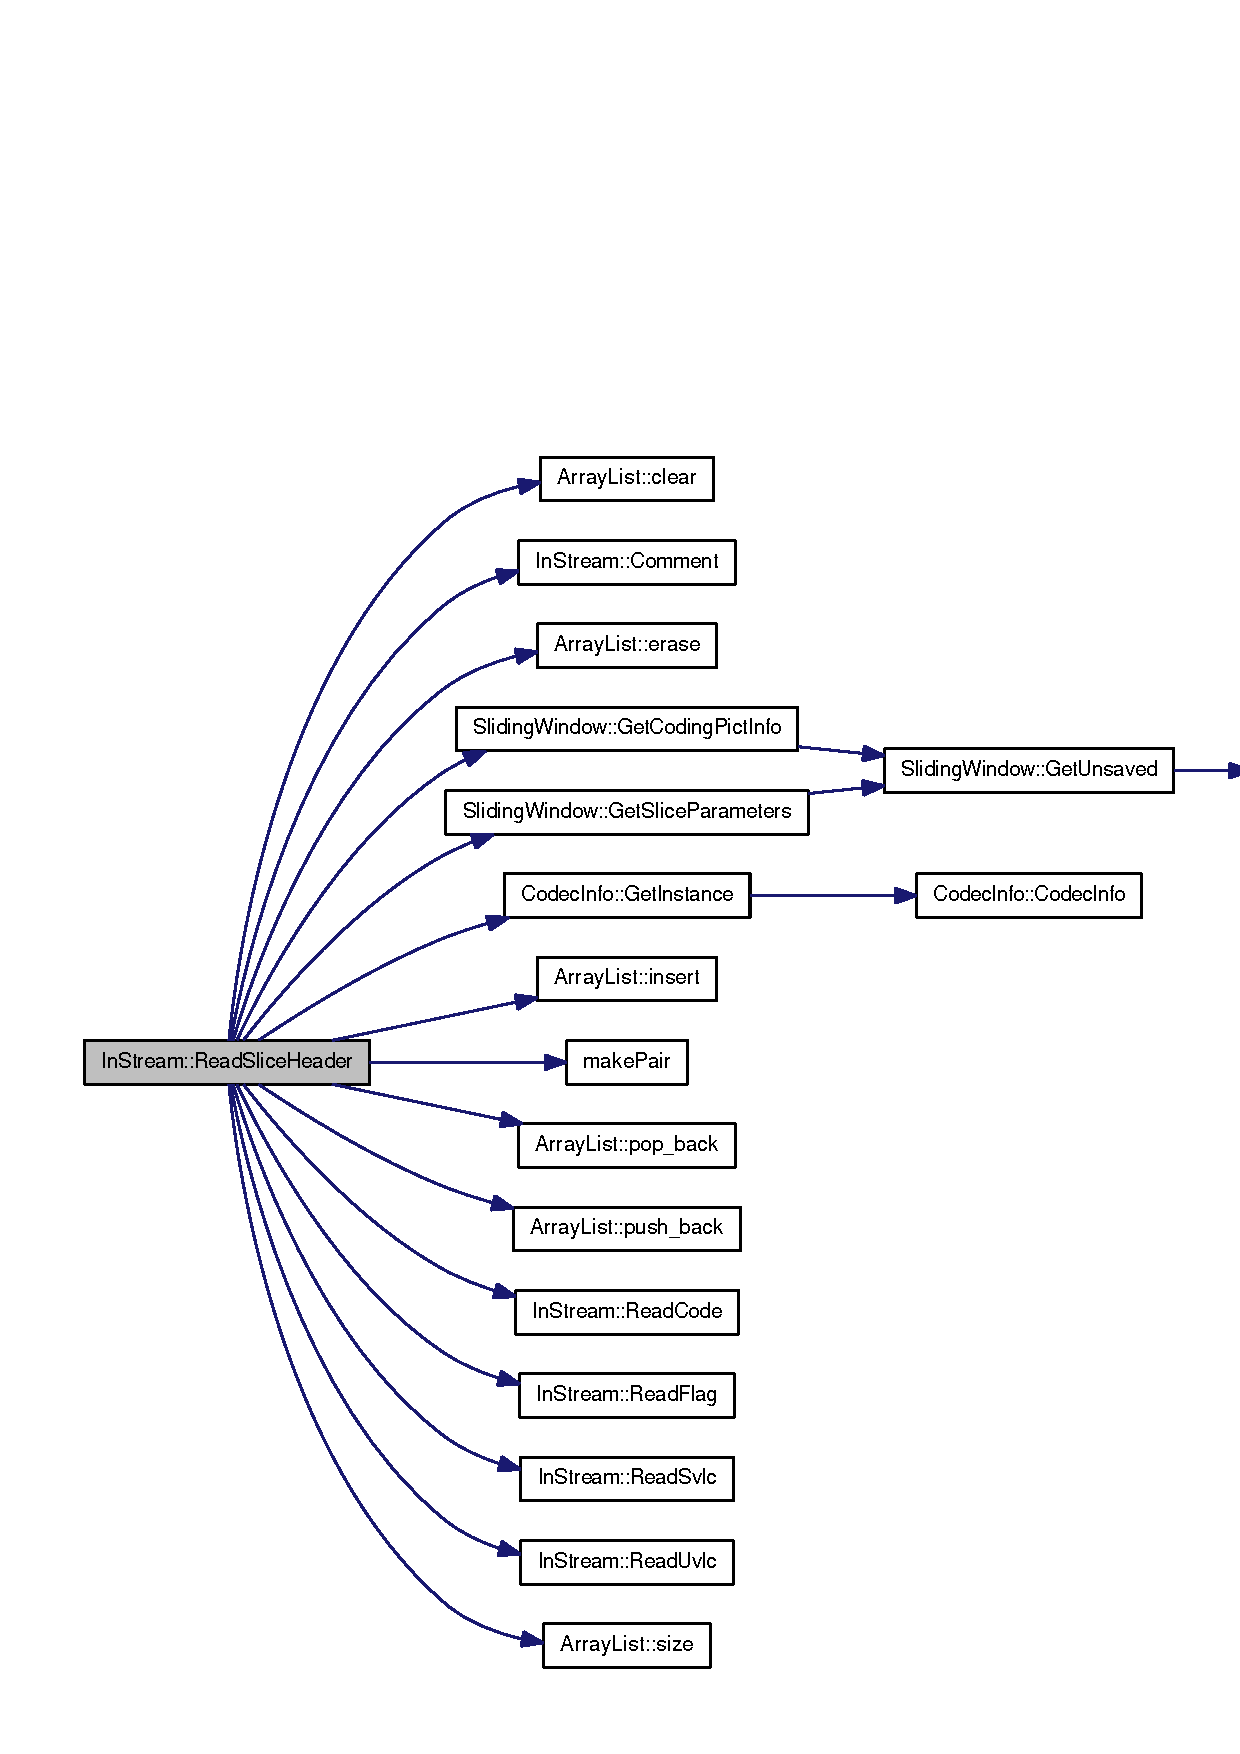
\includegraphics[width=420pt]{class_in_stream_a6369ed63c0fad1007f16e3e885825aea_cgraph}
\end{center}
\end{figure}


\hypertarget{class_in_stream_ab40abe55d480a2dc42e484a8a7eb53a4}{
\index{InStream@{InStream}!ReadSlicePrefix@{ReadSlicePrefix}}
\index{ReadSlicePrefix@{ReadSlicePrefix}!InStream@{InStream}}
\subsubsection[{ReadSlicePrefix}]{\setlength{\rightskip}{0pt plus 5cm}void InStream::ReadSlicePrefix ({\bf SliceParameters} \& {\em sp}, \/  const {\bf SequenceParametersSet} \& {\em sps})}}
\label{class_in_stream_ab40abe55d480a2dc42e484a8a7eb53a4}




\begin{footnotesize}\begin{alltt}
00550 \{
00551         \hyperlink{class_in_stream_acab96485c6978e95e5ef747ebedf09d6}{Comment}(\textcolor{stringliteral}{"NALU HEADER: forbidden\_zero\_bit"});
00552         \hyperlink{_debug_8h_a101586fab2b90a8adffe50a3550e235d}{ASSERT}(\hyperlink{class_in_stream_a340f8fadf6dfc7d17236b15285bba96f}{ReadFlag}() == 0);
00553         \hyperlink{class_in_stream_acab96485c6978e95e5ef747ebedf09d6}{Comment}(\textcolor{stringliteral}{"NALU HEADER: nal\_ref\_idc"});
00554         \hyperlink{class_in_stream_a07d84696f5dd53b6bbc881dc7507de4c}{ReadCode}(2);
00555         \hyperlink{class_in_stream_acab96485c6978e95e5ef747ebedf09d6}{Comment}(\textcolor{stringliteral}{"NALU HEADER: nal\_unit\_type"});
00556         \hyperlink{_debug_8h_a101586fab2b90a8adffe50a3550e235d}{ASSERT}(\hyperlink{class_in_stream_a07d84696f5dd53b6bbc881dc7507de4c}{ReadCode}(5) == \hyperlink{_consts4_standard_8h_a0ae628337fb17a2b11855dd3524f3d04a8c5dfdeb9a126add31b57b718eb32b46}{NAL_UNIT_CODED_SLICE_PREFIX});
00557         \hyperlink{class_in_stream_acab96485c6978e95e5ef747ebedf09d6}{Comment}(\textcolor{stringliteral}{"NALU HEADER: svc\_mvc\_flag"});
00558         \hyperlink{_debug_8h_a101586fab2b90a8adffe50a3550e235d}{ASSERT}(\hyperlink{class_in_stream_a340f8fadf6dfc7d17236b15285bba96f}{ReadFlag}() == 0);
00559         \hyperlink{class_in_stream_acab96485c6978e95e5ef747ebedf09d6}{Comment}(\textcolor{stringliteral}{"NALU HEADER: non\_idr\_flag"});
00560         sp.\hyperlink{struct_slice_parameters_a60f8fe21acd611ec6892e47a2c6029e3}{IDR} = (\hyperlink{class_in_stream_a340f8fadf6dfc7d17236b15285bba96f}{ReadFlag}() == 0);
00561         \hyperlink{class_in_stream_acab96485c6978e95e5ef747ebedf09d6}{Comment}(\textcolor{stringliteral}{"NALU HEADER: priority\_id"});
00562         sp.\hyperlink{struct_slice_parameters_a82aa216a74ffaa7d1859aa1cfe135a8b}{priority_id} = \hyperlink{class_in_stream_a07d84696f5dd53b6bbc881dc7507de4c}{ReadCode}(6);
00563         \hyperlink{class_in_stream_acab96485c6978e95e5ef747ebedf09d6}{Comment}(\textcolor{stringliteral}{"NALU HEADER: view\_id"});
00564         sp.\hyperlink{struct_slice_parameters_ae570f1ba10b1e091c7519264534a7143}{viewId} = \hyperlink{class_in_stream_a07d84696f5dd53b6bbc881dc7507de4c}{ReadCode}(10);
00565         \hyperlink{class_in_stream_acab96485c6978e95e5ef747ebedf09d6}{Comment}(\textcolor{stringliteral}{"NALU HEADER: temporal\_id"});
00566         \textcolor{keywordtype}{int} temporal\_id = \hyperlink{class_in_stream_a07d84696f5dd53b6bbc881dc7507de4c}{ReadCode}(3);
00567         \hyperlink{class_in_stream_acab96485c6978e95e5ef747ebedf09d6}{Comment}(\textcolor{stringliteral}{"NALU HEADER: anchor\_pic\_flag"});
00568         sp.\hyperlink{struct_slice_parameters_af8a7ea94e92b177c38277af8b827eb62}{isAnchor} = (\hyperlink{class_in_stream_a07d84696f5dd53b6bbc881dc7507de4c}{ReadCode}(1) == 1);
00569         \hyperlink{class_in_stream_acab96485c6978e95e5ef747ebedf09d6}{Comment}(\textcolor{stringliteral}{"NALU HEADER: inter\_view\_flag"});
00570         \textcolor{keywordtype}{int} inter\_view = \hyperlink{class_in_stream_a07d84696f5dd53b6bbc881dc7507de4c}{ReadCode}(1);
00571         \hyperlink{class_in_stream_acab96485c6978e95e5ef747ebedf09d6}{Comment}(\textcolor{stringliteral}{"NALU HEADER: reserved\_zero\_one\_bit"});
00572         \hyperlink{class_in_stream_a07d84696f5dd53b6bbc881dc7507de4c}{ReadCode}(1);
00573 \}
\end{alltt}\end{footnotesize}




Here is the call graph for this function:\nopagebreak
\begin{figure}[H]
\begin{center}
\leavevmode
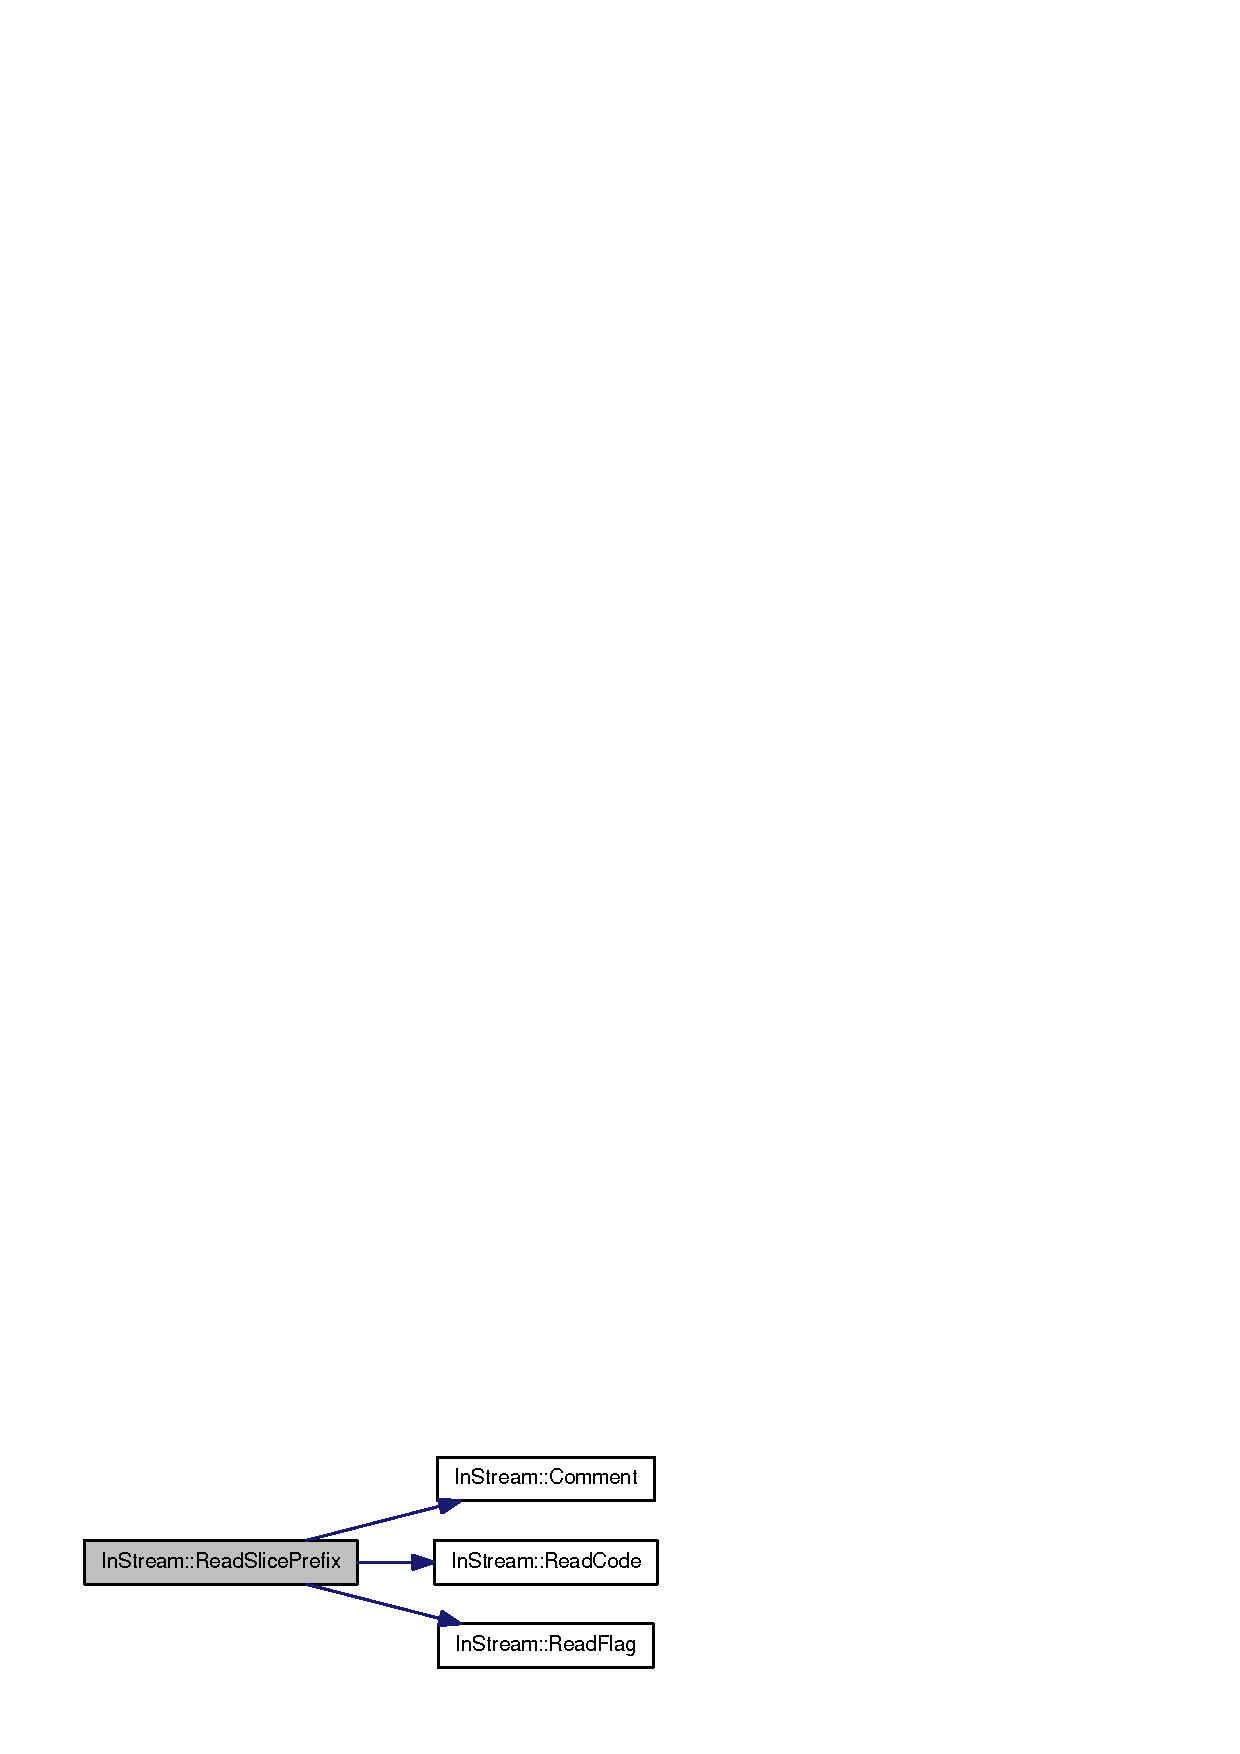
\includegraphics[width=160pt]{class_in_stream_ab40abe55d480a2dc42e484a8a7eb53a4_cgraph}
\end{center}
\end{figure}


\hypertarget{class_in_stream_abb8e8d2b7eef014e7b6285e130a19a0a}{
\index{InStream@{InStream}!ReadSubsetSequenceParameterSet@{ReadSubsetSequenceParameterSet}}
\index{ReadSubsetSequenceParameterSet@{ReadSubsetSequenceParameterSet}!InStream@{InStream}}
\subsubsection[{ReadSubsetSequenceParameterSet}]{\setlength{\rightskip}{0pt plus 5cm}void InStream::ReadSubsetSequenceParameterSet ({\bf SequenceParametersSet} \& {\em sps})}}
\label{class_in_stream_abb8e8d2b7eef014e7b6285e130a19a0a}




\begin{footnotesize}\begin{alltt}
00319 \{
00320         \hyperlink{class_in_stream_acab96485c6978e95e5ef747ebedf09d6}{Comment}(\textcolor{stringliteral}{"NALU HEADER: forbidden\_zero\_bit"});
00321         \hyperlink{_debug_8h_a101586fab2b90a8adffe50a3550e235d}{ASSERT}(\hyperlink{class_in_stream_a340f8fadf6dfc7d17236b15285bba96f}{ReadFlag}() == 0);
00322         \hyperlink{class_in_stream_acab96485c6978e95e5ef747ebedf09d6}{Comment}(\textcolor{stringliteral}{"NALU HEADER: nal\_ref\_idc"});
00323         \hyperlink{_debug_8h_a101586fab2b90a8adffe50a3550e235d}{ASSERT}(\hyperlink{class_in_stream_a07d84696f5dd53b6bbc881dc7507de4c}{ReadCode}(2) == 3);
00324         \hyperlink{class_in_stream_acab96485c6978e95e5ef747ebedf09d6}{Comment}(\textcolor{stringliteral}{"NALU HEADER: nal\_unit\_type"});
00325         \hyperlink{_debug_8h_a101586fab2b90a8adffe50a3550e235d}{ASSERT}(\hyperlink{class_in_stream_a07d84696f5dd53b6bbc881dc7507de4c}{ReadCode}(5) == \hyperlink{_consts4_standard_8h_a0ae628337fb17a2b11855dd3524f3d04ac483bd065332f7337e31c959e7034e6f}{NAL_UNIT_SUBSET_SPS});
00326 
00327         \hyperlink{class_in_stream_acab96485c6978e95e5ef747ebedf09d6}{Comment}(\textcolor{stringliteral}{"SPS: profile\_idc"});
00328         \hyperlink{_debug_8h_a101586fab2b90a8adffe50a3550e235d}{ASSERT}(\hyperlink{class_in_stream_a07d84696f5dd53b6bbc881dc7507de4c}{ReadCode}(8) == \hyperlink{_consts4_standard_8h_a85b10143618f300ff4f5bc6d45c72c01ae06b14698b010f54b54227d57c5bc275}{MULTI_VIEW_PROFILE});
00329         \hyperlink{class_in_stream_acab96485c6978e95e5ef747ebedf09d6}{Comment}(\textcolor{stringliteral}{"SPS: constrained\_set0\_flag"});
00330         \hyperlink{class_in_stream_a340f8fadf6dfc7d17236b15285bba96f}{ReadFlag}();
00331         \hyperlink{class_in_stream_acab96485c6978e95e5ef747ebedf09d6}{Comment}(\textcolor{stringliteral}{"SPS: constrained\_set1\_flag"});
00332         \hyperlink{class_in_stream_a340f8fadf6dfc7d17236b15285bba96f}{ReadFlag}();
00333         \hyperlink{class_in_stream_acab96485c6978e95e5ef747ebedf09d6}{Comment}(\textcolor{stringliteral}{"SPS: constrained\_set2\_flag"});
00334         \hyperlink{class_in_stream_a340f8fadf6dfc7d17236b15285bba96f}{ReadFlag}();
00335         \hyperlink{class_in_stream_acab96485c6978e95e5ef747ebedf09d6}{Comment}(\textcolor{stringliteral}{"SPS: constrained\_set3\_flag"});
00336         \hyperlink{class_in_stream_a340f8fadf6dfc7d17236b15285bba96f}{ReadFlag}();
00337         \hyperlink{class_in_stream_acab96485c6978e95e5ef747ebedf09d6}{Comment}(\textcolor{stringliteral}{"SPS: constrained\_set4\_flag"});
00338         \hyperlink{class_in_stream_a340f8fadf6dfc7d17236b15285bba96f}{ReadFlag}();
00339         \hyperlink{class_in_stream_acab96485c6978e95e5ef747ebedf09d6}{Comment}(\textcolor{stringliteral}{"SPS: constrained\_set5\_flag"});
00340         \hyperlink{class_in_stream_a340f8fadf6dfc7d17236b15285bba96f}{ReadFlag}();
00341         \hyperlink{class_in_stream_acab96485c6978e95e5ef747ebedf09d6}{Comment}(\textcolor{stringliteral}{"SPS: reserved\_zero\_2bits"});
00342         \hyperlink{_debug_8h_a101586fab2b90a8adffe50a3550e235d}{ASSERT}(\hyperlink{class_in_stream_a07d84696f5dd53b6bbc881dc7507de4c}{ReadCode}(2) == 0);
00343         \hyperlink{class_in_stream_acab96485c6978e95e5ef747ebedf09d6}{Comment}(\textcolor{stringliteral}{"SPS: level\_idc"});
00344         \textcolor{keywordtype}{int} level\_idc = \hyperlink{class_in_stream_a07d84696f5dd53b6bbc881dc7507de4c}{ReadCode}(8);
00345         \hyperlink{_debug_8h_a101586fab2b90a8adffe50a3550e235d}{ASSERT}(level\_idc==13 || level\_idc==31 || level\_idc==30 || level\_idc==21);
      
00346         \hyperlink{class_in_stream_acab96485c6978e95e5ef747ebedf09d6}{Comment}(\textcolor{stringliteral}{"SPS: seq\_parameter\_set\_id"});
00347         \hyperlink{class_in_stream_a8e8daf92cb96e583662cafdaf211093c}{ReadUvlc}();
00348 
00349         \textcolor{keywordflow}{if} (sps.\hyperlink{struct_sequence_parameters_set_a53070cb0140d170507760e8422f2ef74}{profileIdc} == 100 || 
00350                 sps.\hyperlink{struct_sequence_parameters_set_a53070cb0140d170507760e8422f2ef74}{profileIdc} == 110 || 
00351                 sps.\hyperlink{struct_sequence_parameters_set_a53070cb0140d170507760e8422f2ef74}{profileIdc} == 122 || 
00352                 sps.\hyperlink{struct_sequence_parameters_set_a53070cb0140d170507760e8422f2ef74}{profileIdc} == 244 || 
00353                 sps.\hyperlink{struct_sequence_parameters_set_a53070cb0140d170507760e8422f2ef74}{profileIdc} == 44 || 
00354                 sps.\hyperlink{struct_sequence_parameters_set_a53070cb0140d170507760e8422f2ef74}{profileIdc} == 83 || 
00355                 sps.\hyperlink{struct_sequence_parameters_set_a53070cb0140d170507760e8422f2ef74}{profileIdc} == 86 || 
00356                 sps.\hyperlink{struct_sequence_parameters_set_a53070cb0140d170507760e8422f2ef74}{profileIdc} == 118 ||
00357                 sps.\hyperlink{struct_sequence_parameters_set_a53070cb0140d170507760e8422f2ef74}{profileIdc} == 128
00358                 ) \{
00359                         \hyperlink{class_in_stream_acab96485c6978e95e5ef747ebedf09d6}{Comment}(\textcolor{stringliteral}{"--- fidelity range extension syntax ---"});
00360                         \hyperlink{class_in_stream_acab96485c6978e95e5ef747ebedf09d6}{Comment}(\textcolor{stringliteral}{"ReadFrext"});
00361                         \hyperlink{class_in_stream_acab96485c6978e95e5ef747ebedf09d6}{Comment}(\textcolor{stringliteral}{"SPS: chroma\_format\_idc"});
00362                         \textcolor{comment}{//sps.chromaFormatIdc = ReadUvlc();}
00363                         \hyperlink{_debug_8h_a101586fab2b90a8adffe50a3550e235d}{ASSERT}(\hyperlink{class_in_stream_a8e8daf92cb96e583662cafdaf211093c}{ReadUvlc}() == 1); \textcolor{comment}{// 4:2:0 chroma\_format\_idc=1}
00364                         \textcolor{comment}{//chroma\_format\_idc ��ָ��6.2 ��������ģ�������ȡ����Ӧ��ɫ��ȡ����chroma\_form
      at\_idc ��ֵӦ����0}
00365                         \textcolor{comment}{//��3�ķ�Χ�ڣ�����0��3������chroma\_format\_idc������ʱ��Ӧ�ƶ���ֵΪ1��4��2��0��ɫ�ȸ�ʽ
      ����}
00366                         \hyperlink{class_in_stream_acab96485c6978e95e5ef747ebedf09d6}{Comment}(\textcolor{stringliteral}{"SPS: bit\_depth\_luma\_minus8"});
00367                         \hyperlink{_debug_8h_a101586fab2b90a8adffe50a3550e235d}{ASSERT}(\hyperlink{class_in_stream_a8e8daf92cb96e583662cafdaf211093c}{ReadUvlc}() == 0); \textcolor{comment}{// BitDepthY = 8 + bit\_depth\_lum
      a\_minus8,  QpBdOffsetY = 6 * bit\_depth\_luma\_minus8 bit\_depth\_luma\_minus8=0}
00368                         \hyperlink{class_in_stream_acab96485c6978e95e5ef747ebedf09d6}{Comment}(\textcolor{stringliteral}{"SPS: bit\_depth\_chroma\_minus8"});
00369                         \hyperlink{_debug_8h_a101586fab2b90a8adffe50a3550e235d}{ASSERT}(\hyperlink{class_in_stream_a8e8daf92cb96e583662cafdaf211093c}{ReadUvlc}() == 0); \textcolor{comment}{// BitDepthC = 8 + bit\_depth\_chr
      oma\_minus8,  QpBdOffsetC = 6 * ( bit\_depth\_chroma\_minus8 + residual\_colour\_transf
      orm\_flag) bit\_depth\_chroma\_minus8=0}
00370                         \hyperlink{class_in_stream_acab96485c6978e95e5ef747ebedf09d6}{Comment}(\textcolor{stringliteral}{"SPS: qpprime\_y\_zero\_transform\_bypass\_flag"});
00371                         \hyperlink{_debug_8h_a101586fab2b90a8adffe50a3550e235d}{ASSERT}(\hyperlink{class_in_stream_a340f8fadf6dfc7d17236b15285bba96f}{ReadFlag}() == 0);\textcolor{comment}{//qpprime\_y\_zero\_transform\_bypass
      \_flag = 0}
00372                         \hyperlink{class_in_stream_acab96485c6978e95e5ef747ebedf09d6}{Comment}(\textcolor{stringliteral}{"SPS: seq\_scaling\_matrix\_present\_flag"});
00373                         \hyperlink{_debug_8h_a101586fab2b90a8adffe50a3550e235d}{ASSERT}(\hyperlink{class_in_stream_a340f8fadf6dfc7d17236b15285bba96f}{ReadFlag}() == 0);\textcolor{comment}{//seq\_scaling\_matrix\_present\_flag
      =0}
00374         \}
00375 
00376         \textcolor{keywordtype}{int} log2nFramesM4 = \hyperlink{class_in_stream_a8e8daf92cb96e583662cafdaf211093c}{ReadUvlc}();
00377         sps.\hyperlink{struct_sequence_parameters_set_ac5f0d82a961acfe4f966e7c35aa37339}{log2nFrames} = log2nFramesM4 + 4;
00378         sps.\hyperlink{struct_sequence_parameters_set_afedac9d01de6ec718715ab45c63ee999}{nFramesM1} = (1<<sps.\hyperlink{struct_sequence_parameters_set_ac5f0d82a961acfe4f966e7c35aa37339}{log2nFrames})-1;
00379 
00380         \hyperlink{class_in_stream_acab96485c6978e95e5ef747ebedf09d6}{Comment}(\textcolor{stringliteral}{"SPS: pic\_order\_cnt\_type"});
00381         \textcolor{keywordtype}{int} picOrderCntType = 0;
00382         \hyperlink{_debug_8h_a101586fab2b90a8adffe50a3550e235d}{ASSERT}(\hyperlink{class_in_stream_a8e8daf92cb96e583662cafdaf211093c}{ReadUvlc}() == picOrderCntType);
00383         \hyperlink{class_in_stream_acab96485c6978e95e5ef747ebedf09d6}{Comment}(\textcolor{stringliteral}{"SPS: log2\_max\_pic\_order\_cnt\_lsb\_minus4"});
00384         \textcolor{keywordtype}{int} log2nPocM4 = \hyperlink{class_in_stream_a8e8daf92cb96e583662cafdaf211093c}{ReadUvlc}();
00385         sps.\hyperlink{struct_sequence_parameters_set_aff653fc637f7290b7edbaf1cfeacd6ca}{log2nPoc} = log2nPocM4 + 4;
00386         sps.\hyperlink{struct_sequence_parameters_set_a786d1401a47490d15c7f1512e21994ce}{nPocM1} = (1<<sps.\hyperlink{struct_sequence_parameters_set_aff653fc637f7290b7edbaf1cfeacd6ca}{log2nPoc}) - 1;
00387 
00388         \hyperlink{class_in_stream_acab96485c6978e95e5ef747ebedf09d6}{Comment}(\textcolor{stringliteral}{"SPS: num\_ref\_frames"});
00389         \hyperlink{class_in_stream_a8e8daf92cb96e583662cafdaf211093c}{ReadUvlc}();
00390         \hyperlink{class_in_stream_acab96485c6978e95e5ef747ebedf09d6}{Comment}(\textcolor{stringliteral}{"SPS: required\_frame\_num\_update\_behaviour\_flag"});
00391         \hyperlink{_debug_8h_a101586fab2b90a8adffe50a3550e235d}{ASSERT}(\hyperlink{class_in_stream_a340f8fadf6dfc7d17236b15285bba96f}{ReadFlag}() == 1);
00392 
00393         \hyperlink{class_in_stream_acab96485c6978e95e5ef747ebedf09d6}{Comment}(\textcolor{stringliteral}{"SPS: pic\_width\_in\_mbs\_minus\_1"});
00394         \hyperlink{_debug_8h_a101586fab2b90a8adffe50a3550e235d}{ASSERT}(\hyperlink{class_in_stream_a8e8daf92cb96e583662cafdaf211093c}{ReadUvlc}() == (sps.\hyperlink{struct_sequence_parameters_set_a72286e512a40a01670e2519b3971cee2}{width}>>4)-1);
00395         \hyperlink{class_in_stream_acab96485c6978e95e5ef747ebedf09d6}{Comment}(\textcolor{stringliteral}{"SPS: pic\_height\_in\_mbs\_units\_minus\_1"});
00396         \hyperlink{_debug_8h_a101586fab2b90a8adffe50a3550e235d}{ASSERT}(\hyperlink{class_in_stream_a8e8daf92cb96e583662cafdaf211093c}{ReadUvlc}() == (sps.\hyperlink{struct_sequence_parameters_set_ab3b7bd818f9a0d1456d92496473a42eb}{height}>>4) - 1);
00397         \hyperlink{class_in_stream_acab96485c6978e95e5ef747ebedf09d6}{Comment}(\textcolor{stringliteral}{"SPS: frame\_mbs\_only\_flag"});
00398         \hyperlink{_debug_8h_a101586fab2b90a8adffe50a3550e235d}{ASSERT}(\hyperlink{class_in_stream_a340f8fadf6dfc7d17236b15285bba96f}{ReadFlag}() == 1);
00399         \hyperlink{class_in_stream_acab96485c6978e95e5ef747ebedf09d6}{Comment}(\textcolor{stringliteral}{"SPS: direct\_8x8\_inference\_flag"});
00400         \hyperlink{_debug_8h_a101586fab2b90a8adffe50a3550e235d}{ASSERT}(\hyperlink{class_in_stream_a340f8fadf6dfc7d17236b15285bba96f}{ReadFlag}() == 1);
00401         \hyperlink{class_in_stream_acab96485c6978e95e5ef747ebedf09d6}{Comment}(\textcolor{stringliteral}{"SPS: frame\_cropping\_flag"});
00402         \hyperlink{_debug_8h_a101586fab2b90a8adffe50a3550e235d}{ASSERT}(\hyperlink{class_in_stream_a340f8fadf6dfc7d17236b15285bba96f}{ReadFlag}() == 0);
00403         \hyperlink{class_in_stream_acab96485c6978e95e5ef747ebedf09d6}{Comment}(\textcolor{stringliteral}{"SPS: vui\_parameters\_present\_flag"});
00404         sps.\hyperlink{struct_sequence_parameters_set_a557345c281f445eb71cbcd5d72a9aed0}{vui_parameters_present} = \hyperlink{class_in_stream_a340f8fadf6dfc7d17236b15285bba96f}{ReadFlag}();
00405         \textcolor{keywordflow}{if} (sps.\hyperlink{struct_sequence_parameters_set_a557345c281f445eb71cbcd5d72a9aed0}{vui_parameters_present})
00406         \{
00407                 readVuiParameters(sps.\hyperlink{struct_sequence_parameters_set_ac473de5b97f08fefdbe39fe9c2c2c846}{vuiparams});
00408         \}
00409 
00410         \hyperlink{class_in_stream_acab96485c6978e95e5ef747ebedf09d6}{Comment}(\textcolor{stringliteral}{"SUBSET SPS: bit\_equal\_to\_one"});
00411         \hyperlink{_debug_8h_a101586fab2b90a8adffe50a3550e235d}{ASSERT}(\hyperlink{class_in_stream_a340f8fadf6dfc7d17236b15285bba96f}{ReadFlag}() == 1);
00412 
00413         \hyperlink{class_in_stream_acab96485c6978e95e5ef747ebedf09d6}{Comment}(\textcolor{stringliteral}{"SPS: num\_views\_minus\_1"});
00414         sps.\hyperlink{struct_sequence_parameters_set_af32c7819f630856ccd99aaf78e8f656c}{viewCount} = \hyperlink{class_in_stream_a8e8daf92cb96e583662cafdaf211093c}{ReadUvlc}() + 1;
00415 
00416         sps.\hyperlink{struct_sequence_parameters_set_a082e13208bc0afd9377676e156e750b4}{viewCodingOrder}.\hyperlink{class_array_list_acb53d54675318c94332d0ec8b6819eb3}{clear}();
00417         \textcolor{keywordflow}{for} (\textcolor{keywordtype}{int} i = 0; i < sps.\hyperlink{struct_sequence_parameters_set_af32c7819f630856ccd99aaf78e8f656c}{viewCount}; ++i)
00418         \{
00419                 \hyperlink{class_in_stream_acab96485c6978e95e5ef747ebedf09d6}{Comment}(\textcolor{stringliteral}{"SPS: view\_id[i]"});
00420                 sps.\hyperlink{struct_sequence_parameters_set_a082e13208bc0afd9377676e156e750b4}{viewCodingOrder}.\hyperlink{class_array_list_a7b5376678a9b5af0e0ed913fbe04b902}{push_back}(\hyperlink{class_in_stream_a8e8daf92cb96e583662cafdaf211093c}{ReadUvlc}());
00421         \}
00422 
00423         sps.\hyperlink{struct_sequence_parameters_set_ae9b6a7d85da9fec255cca59c3d750ecd}{anchorRefsList0}.\hyperlink{class_array_list_acb53d54675318c94332d0ec8b6819eb3}{clear}();
00424         \hyperlink{class_array_list}{ArrayList<int>} tmp;
00425         \textcolor{keywordflow}{for} (\textcolor{keywordtype}{int} i = 0; i < sps.\hyperlink{struct_sequence_parameters_set_af32c7819f630856ccd99aaf78e8f656c}{viewCount}; ++i)
00426         \{
00427                 sps.\hyperlink{struct_sequence_parameters_set_ae9b6a7d85da9fec255cca59c3d750ecd}{anchorRefsList0}.\hyperlink{class_array_list_a7b5376678a9b5af0e0ed913fbe04b902}{push_back}(tmp);
00428         \}
00429         sps.\hyperlink{struct_sequence_parameters_set_a7b865f89c34428785081c3c4acadc965}{anchorRefsList1} = sps.\hyperlink{struct_sequence_parameters_set_ae9b6a7d85da9fec255cca59c3d750ecd}{anchorRefsList0};
00430         sps.\hyperlink{struct_sequence_parameters_set_ab9b078b23e746ef60f7697896b963b93}{nonAnchorRefsList0} = sps.\hyperlink{struct_sequence_parameters_set_ae9b6a7d85da9fec255cca59c3d750ecd}{anchorRefsList0};
00431         sps.\hyperlink{struct_sequence_parameters_set_a68b7ffb23b151c53312798f7ab79a67a}{nonAnchorRefsList1} = sps.\hyperlink{struct_sequence_parameters_set_ae9b6a7d85da9fec255cca59c3d750ecd}{anchorRefsList0};
00432         \textcolor{keywordflow}{for} (\textcolor{keywordtype}{int} i = 1; i < sps.\hyperlink{struct_sequence_parameters_set_af32c7819f630856ccd99aaf78e8f656c}{viewCount}; ++i)
00433         \{
00434                 \textcolor{keywordtype}{int} coding = sps.\hyperlink{struct_sequence_parameters_set_a082e13208bc0afd9377676e156e750b4}{viewCodingOrder}[i];
00435                 \hyperlink{class_in_stream_acab96485c6978e95e5ef747ebedf09d6}{Comment}(\textcolor{stringliteral}{"SPS: num\_anchor\_refs\_l0[i]"});
00436                 \textcolor{keywordtype}{int} nAnchorRefs = \hyperlink{class_in_stream_a8e8daf92cb96e583662cafdaf211093c}{ReadUvlc}();
00437                 \textcolor{keywordflow}{for} (\textcolor{keywordtype}{int} j = 0; j < nAnchorRefs; ++j)
00438                 \{
00439                         \hyperlink{class_in_stream_acab96485c6978e95e5ef747ebedf09d6}{Comment}(\textcolor{stringliteral}{"SPS: anchor\_ref\_l0[i][j]"});
00440                         \textcolor{keywordtype}{int} refv = \hyperlink{class_in_stream_a8e8daf92cb96e583662cafdaf211093c}{ReadUvlc}();
00441                         sps.\hyperlink{struct_sequence_parameters_set_ae9b6a7d85da9fec255cca59c3d750ecd}{anchorRefsList0}[coding].\hyperlink{class_array_list_a7b5376678a9b5af0e0ed913fbe04b902}{push_back}(refv);
00442                 \}
00443 
00444                 \hyperlink{class_in_stream_acab96485c6978e95e5ef747ebedf09d6}{Comment}(\textcolor{stringliteral}{"SPS: num\_anchor\_refs\_l1[i]"});
00445                 nAnchorRefs = \hyperlink{class_in_stream_a8e8daf92cb96e583662cafdaf211093c}{ReadUvlc}();
00446                 \textcolor{keywordflow}{for} (\textcolor{keywordtype}{int} j = 0; j < nAnchorRefs; ++j)
00447                 \{
00448                         \hyperlink{class_in_stream_acab96485c6978e95e5ef747ebedf09d6}{Comment}(\textcolor{stringliteral}{"SPS: anchor\_ref\_l1[i][j]"});
00449                         \textcolor{keywordtype}{int} refv = \hyperlink{class_in_stream_a8e8daf92cb96e583662cafdaf211093c}{ReadUvlc}();
00450                         sps.\hyperlink{struct_sequence_parameters_set_a7b865f89c34428785081c3c4acadc965}{anchorRefsList1}[coding].\hyperlink{class_array_list_a7b5376678a9b5af0e0ed913fbe04b902}{push_back}(refv);
00451                 \}
00452         \}
00453 
00454         \textcolor{keywordflow}{for} (\textcolor{keywordtype}{int} i = 1; i < sps.\hyperlink{struct_sequence_parameters_set_af32c7819f630856ccd99aaf78e8f656c}{viewCount}; ++i)
00455         \{
00456                 \textcolor{keywordtype}{int} coding = sps.\hyperlink{struct_sequence_parameters_set_a082e13208bc0afd9377676e156e750b4}{viewCodingOrder}[i];
00457                 \hyperlink{class_in_stream_acab96485c6978e95e5ef747ebedf09d6}{Comment}(\textcolor{stringliteral}{"SPS: num\_non\_anchor\_refs\_l0[i]"});
00458                 \textcolor{keywordtype}{int} nAnchorRefs = \hyperlink{class_in_stream_a8e8daf92cb96e583662cafdaf211093c}{ReadUvlc}();
00459                 \textcolor{keywordflow}{for} (\textcolor{keywordtype}{int} j = 0; j < nAnchorRefs; ++j)
00460                 \{
00461                         \hyperlink{class_in_stream_acab96485c6978e95e5ef747ebedf09d6}{Comment}(\textcolor{stringliteral}{"SPS: non\_anchor\_ref\_l0[i][j]"});
00462                         \textcolor{keywordtype}{int} refv = \hyperlink{class_in_stream_a8e8daf92cb96e583662cafdaf211093c}{ReadUvlc}();
00463                         sps.\hyperlink{struct_sequence_parameters_set_ab9b078b23e746ef60f7697896b963b93}{nonAnchorRefsList0}[coding].\hyperlink{class_array_list_a7b5376678a9b5af0e0ed913fbe04b902}{push_back}(refv);
00464                 \}
00465 
00466                 \hyperlink{class_in_stream_acab96485c6978e95e5ef747ebedf09d6}{Comment}(\textcolor{stringliteral}{"SPS: num\_non\_anchor\_refs\_l1[i]"});
00467                 nAnchorRefs = \hyperlink{class_in_stream_a8e8daf92cb96e583662cafdaf211093c}{ReadUvlc}();
00468                 \textcolor{keywordflow}{for} (\textcolor{keywordtype}{int} j = 0; j < nAnchorRefs; ++j)
00469                 \{
00470                         \hyperlink{class_in_stream_acab96485c6978e95e5ef747ebedf09d6}{Comment}(\textcolor{stringliteral}{"SPS: non\_anchor\_ref\_l1[i][j]"});
00471                         \textcolor{keywordtype}{int} refv = \hyperlink{class_in_stream_a8e8daf92cb96e583662cafdaf211093c}{ReadUvlc}();
00472                         sps.\hyperlink{struct_sequence_parameters_set_a68b7ffb23b151c53312798f7ab79a67a}{nonAnchorRefsList1}[coding].\hyperlink{class_array_list_a7b5376678a9b5af0e0ed913fbe04b902}{push_back}(refv);
00473                 \}
00474         \}
00475 
00476         \hyperlink{class_in_stream_acab96485c6978e95e5ef747ebedf09d6}{Comment}(\textcolor{stringliteral}{"SPS: num\_level\_values\_signalled"});
00477         \hyperlink{_debug_8h_a101586fab2b90a8adffe50a3550e235d}{ASSERT}(\hyperlink{class_in_stream_a8e8daf92cb96e583662cafdaf211093c}{ReadUvlc}() == 0);
00478 
00479 \textcolor{comment}{/*}
00480 \textcolor{comment}{        ASSERT(ReadCode(8) == 0);}
00481 \textcolor{comment}{        ASSERT(ReadUvlc() == 0);}
00482 \textcolor{comment}{        ASSERT(ReadCode(3) == 0);}
00483 \textcolor{comment}{        ASSERT(ReadUvlc() == 0);}
00484 \textcolor{comment}{        ASSERT(ReadUvlc() == 0);}
00485 \textcolor{comment}{        ASSERT(ReadUvlc() == 0);}
00486 \textcolor{comment}{*/}
00487 
00488         \hyperlink{class_in_stream_acab96485c6978e95e5ef747ebedf09d6}{Comment}(\textcolor{stringliteral}{"SUBSET SPS: mvc\_vui\_parameters\_present\_flag"});
00489         \hyperlink{_debug_8h_a101586fab2b90a8adffe50a3550e235d}{ASSERT}(\hyperlink{class_in_stream_a340f8fadf6dfc7d17236b15285bba96f}{ReadFlag}() == 0);
00490         \hyperlink{class_in_stream_acab96485c6978e95e5ef747ebedf09d6}{Comment}(\textcolor{stringliteral}{"SUBSET SPS: Additional\_extension2\_flag"});
00491         \hyperlink{_debug_8h_a101586fab2b90a8adffe50a3550e235d}{ASSERT}(\hyperlink{class_in_stream_a340f8fadf6dfc7d17236b15285bba96f}{ReadFlag}() == 0);
00492 \}
\end{alltt}\end{footnotesize}




Here is the call graph for this function:\nopagebreak
\begin{figure}[H]
\begin{center}
\leavevmode
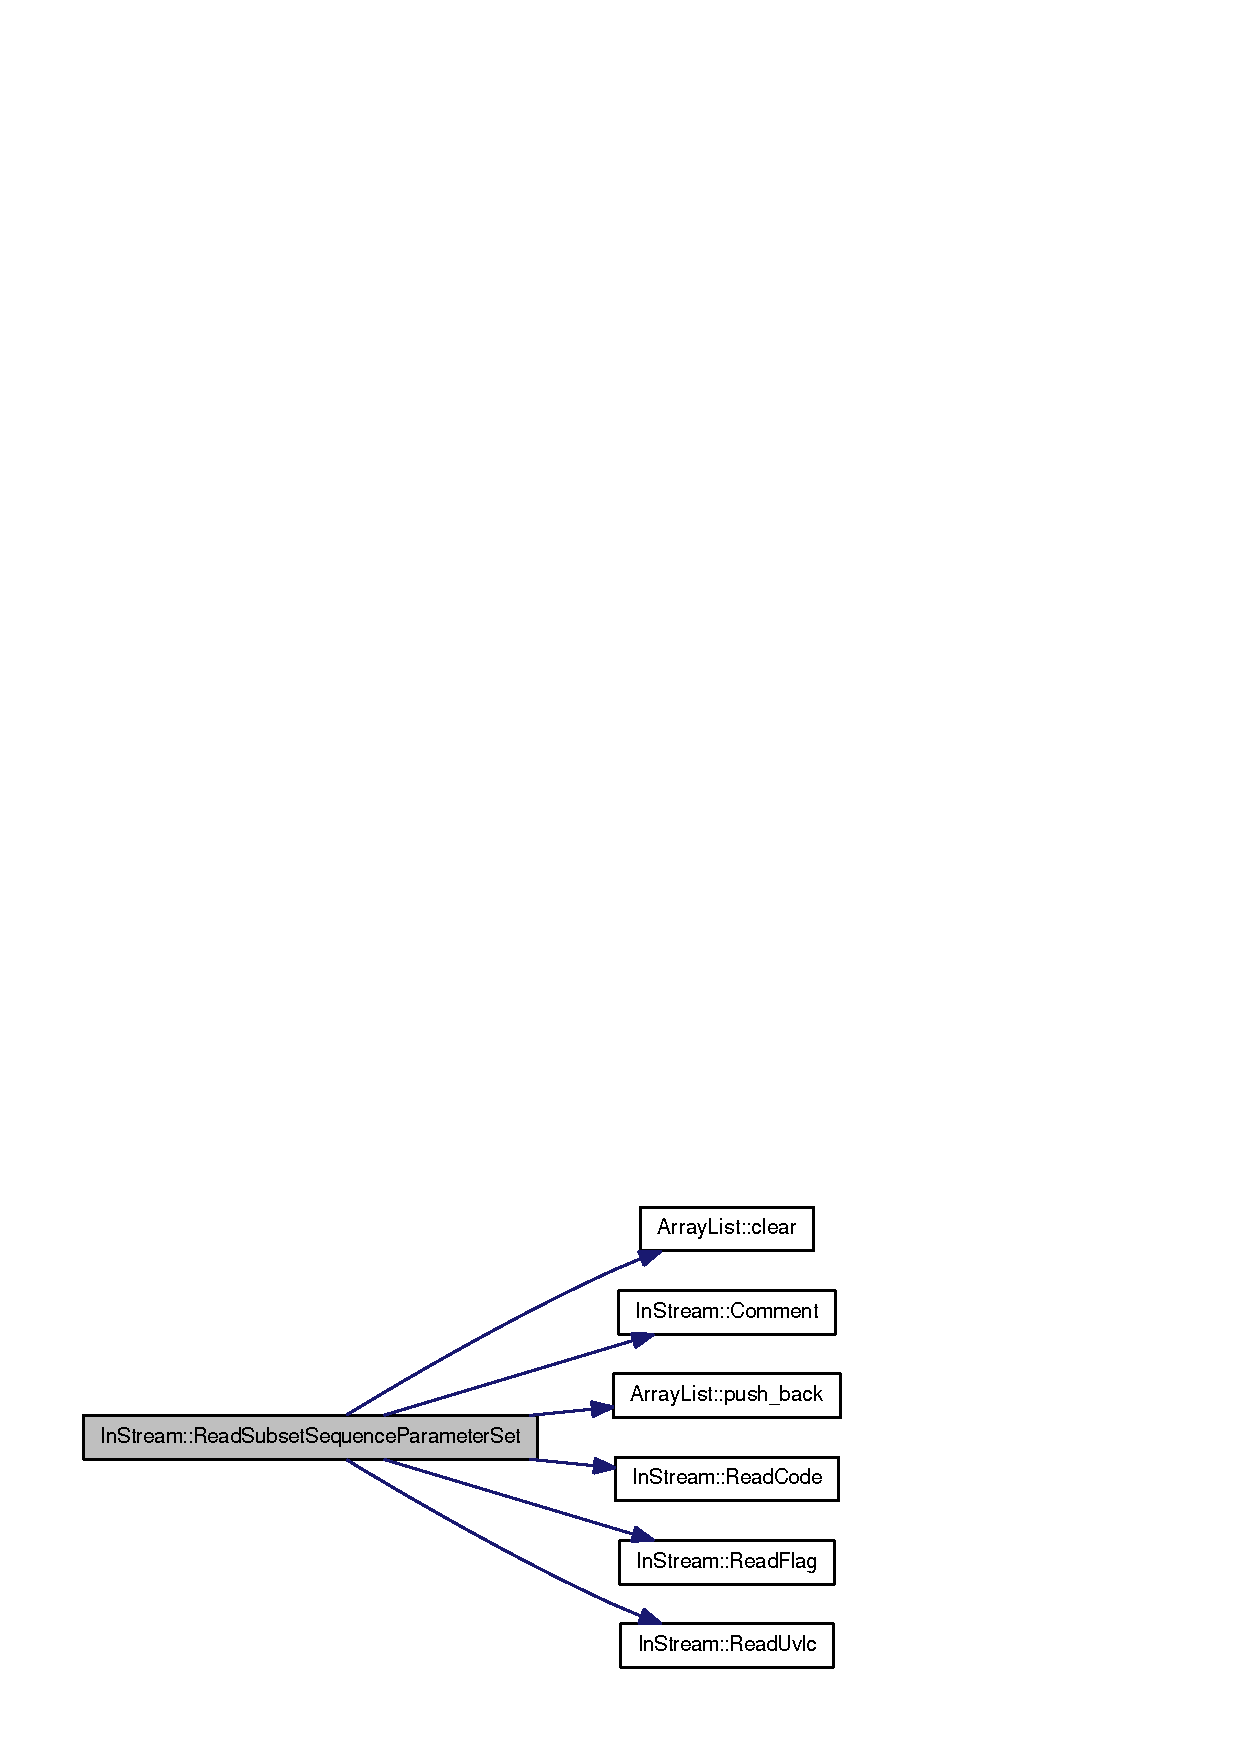
\includegraphics[width=204pt]{class_in_stream_abb8e8d2b7eef014e7b6285e130a19a0a_cgraph}
\end{center}
\end{figure}


\hypertarget{class_in_stream_accc880522e6e43bd3a46297988de1c47}{
\index{InStream@{InStream}!ReadSvlc@{ReadSvlc}}
\index{ReadSvlc@{ReadSvlc}!InStream@{InStream}}
\subsubsection[{ReadSvlc}]{\setlength{\rightskip}{0pt plus 5cm}{\bf int32\_\-t} InStream::ReadSvlc ()}}
\label{class_in_stream_accc880522e6e43bd3a46297988de1c47}




\begin{footnotesize}\begin{alltt}
00051 \{
00052         \hyperlink{_types_8h_a115ba3a1b24a8702355c5dbd61ce01e0}{int32_t} svlc = eg\_read\_se(&bs);
00053         \textcolor{comment}{//printf("Svlc %d\(\backslash\)n", svlc);}
00054         \textcolor{keywordflow}{return} svlc;
00055 \}
\end{alltt}\end{footnotesize}




Here is the caller graph for this function:\nopagebreak
\begin{figure}[H]
\begin{center}
\leavevmode
\includegraphics[width=179pt]{class_in_stream_accc880522e6e43bd3a46297988de1c47_icgraph}
\end{center}
\end{figure}


\hypertarget{class_in_stream_a8e8daf92cb96e583662cafdaf211093c}{
\index{InStream@{InStream}!ReadUvlc@{ReadUvlc}}
\index{ReadUvlc@{ReadUvlc}!InStream@{InStream}}
\subsubsection[{ReadUvlc}]{\setlength{\rightskip}{0pt plus 5cm}{\bf uint32\_\-t} InStream::ReadUvlc ()}}
\label{class_in_stream_a8e8daf92cb96e583662cafdaf211093c}




\begin{footnotesize}\begin{alltt}
00044 \{
00045         \hyperlink{_types_8h_a04909d1366bb244ff2482beb51635f37}{uint32_t} uvlc = \hyperlink{_bitstream_8h_acad61027e3182912d2b9d95180d45250}{eg_read_ue}(&bs);
00046         \textcolor{comment}{//printf("Uvlc %d\(\backslash\)n", uvlc);}
00047         \textcolor{keywordflow}{return} uvlc;
00048 \}
\end{alltt}\end{footnotesize}




Here is the caller graph for this function:\nopagebreak
\begin{figure}[H]
\begin{center}
\leavevmode
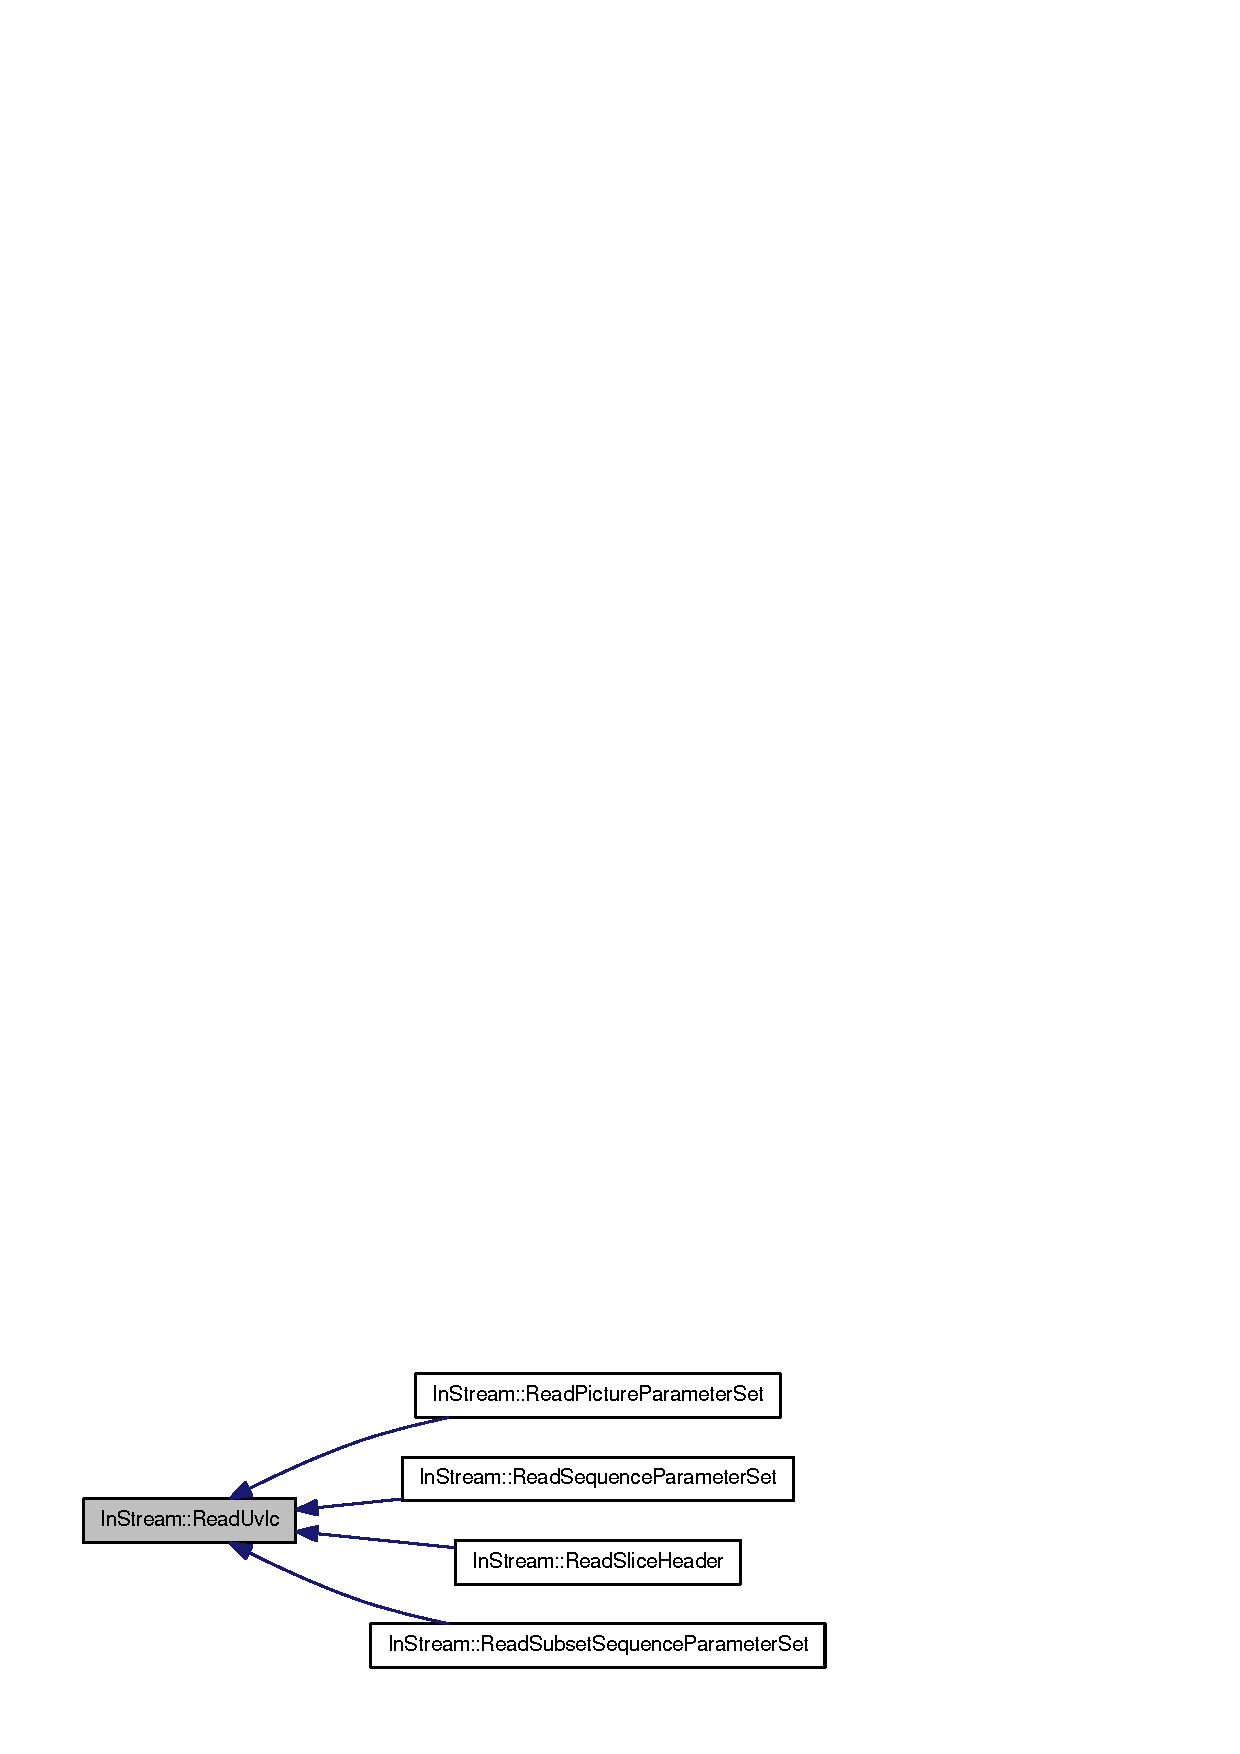
\includegraphics[width=200pt]{class_in_stream_a8e8daf92cb96e583662cafdaf211093c_icgraph}
\end{center}
\end{figure}


\hypertarget{class_in_stream_a700d52a510354fcf7787b118dbeb406f}{
\index{InStream@{InStream}!ResetBitstream@{ResetBitstream}}
\index{ResetBitstream@{ResetBitstream}!InStream@{InStream}}
\subsubsection[{ResetBitstream}]{\setlength{\rightskip}{0pt plus 5cm}void InStream::ResetBitstream ()}}
\label{class_in_stream_a700d52a510354fcf7787b118dbeb406f}




\begin{footnotesize}\begin{alltt}
00063 \{
00064         BitstreamReset(&bs);
00065 \}
\end{alltt}\end{footnotesize}




Here is the caller graph for this function:\nopagebreak
\begin{figure}[H]
\begin{center}
\leavevmode
\includegraphics[width=162pt]{class_in_stream_a700d52a510354fcf7787b118dbeb406f_icgraph}
\end{center}
\end{figure}




The documentation for this class was generated from the following files:\begin{DoxyCompactItemize}
\item 
MVCDecoder/Stream/\hyperlink{_in_stream_8h}{InStream.h}\item 
MVCDecoder/Stream/\hyperlink{_in_stream_8cpp}{InStream.cpp}\end{DoxyCompactItemize}

\hypertarget{structmacroblockdata}{
\section{macroblockdata Struct Reference}
\label{structmacroblockdata}\index{macroblockdata@{macroblockdata}}
}


{\ttfamily \#include $<$Types.h$>$}

\subsection*{Public Attributes}
\begin{DoxyCompactItemize}
\item 
\hyperlink{_types_8h_a15eca744b460ea898a5e04df2899d49f}{macroblockdata\_\-y} \hyperlink{structmacroblockdata_ac3e45382bf0c21b9714fe7d8e9e1a12d}{y}
\item 
\hyperlink{_types_8h_abb0aad4f6cc5fb3beadf8f4df08da50f}{macroblockdata\_\-uv} \hyperlink{structmacroblockdata_a07e17343606921d436bfddef89d0d93f}{uv}
\end{DoxyCompactItemize}


\subsection{Member Data Documentation}
\hypertarget{structmacroblockdata_a07e17343606921d436bfddef89d0d93f}{
\index{macroblockdata@{macroblockdata}!uv@{uv}}
\index{uv@{uv}!macroblockdata@{macroblockdata}}
\subsubsection[{uv}]{\setlength{\rightskip}{0pt plus 5cm}{\bf macroblockdata\_\-uv} {\bf macroblockdata::uv}}}
\label{structmacroblockdata_a07e17343606921d436bfddef89d0d93f}
\hypertarget{structmacroblockdata_ac3e45382bf0c21b9714fe7d8e9e1a12d}{
\index{macroblockdata@{macroblockdata}!y@{y}}
\index{y@{y}!macroblockdata@{macroblockdata}}
\subsubsection[{y}]{\setlength{\rightskip}{0pt plus 5cm}{\bf macroblockdata\_\-y} {\bf macroblockdata::y}}}
\label{structmacroblockdata_ac3e45382bf0c21b9714fe7d8e9e1a12d}


The documentation for this struct was generated from the following file:\begin{DoxyCompactItemize}
\item 
MVCCommonLib/\hyperlink{_types_8h}{Types.h}\end{DoxyCompactItemize}

\hypertarget{structmacroblock_info}{
\section{macroblockInfo Struct Reference}
\label{structmacroblock_info}\index{macroblockInfo@{macroblockInfo}}
}


{\ttfamily \#include $<$Types.h$>$}



Collaboration diagram for macroblockInfo:\nopagebreak
\begin{figure}[H]
\begin{center}
\leavevmode
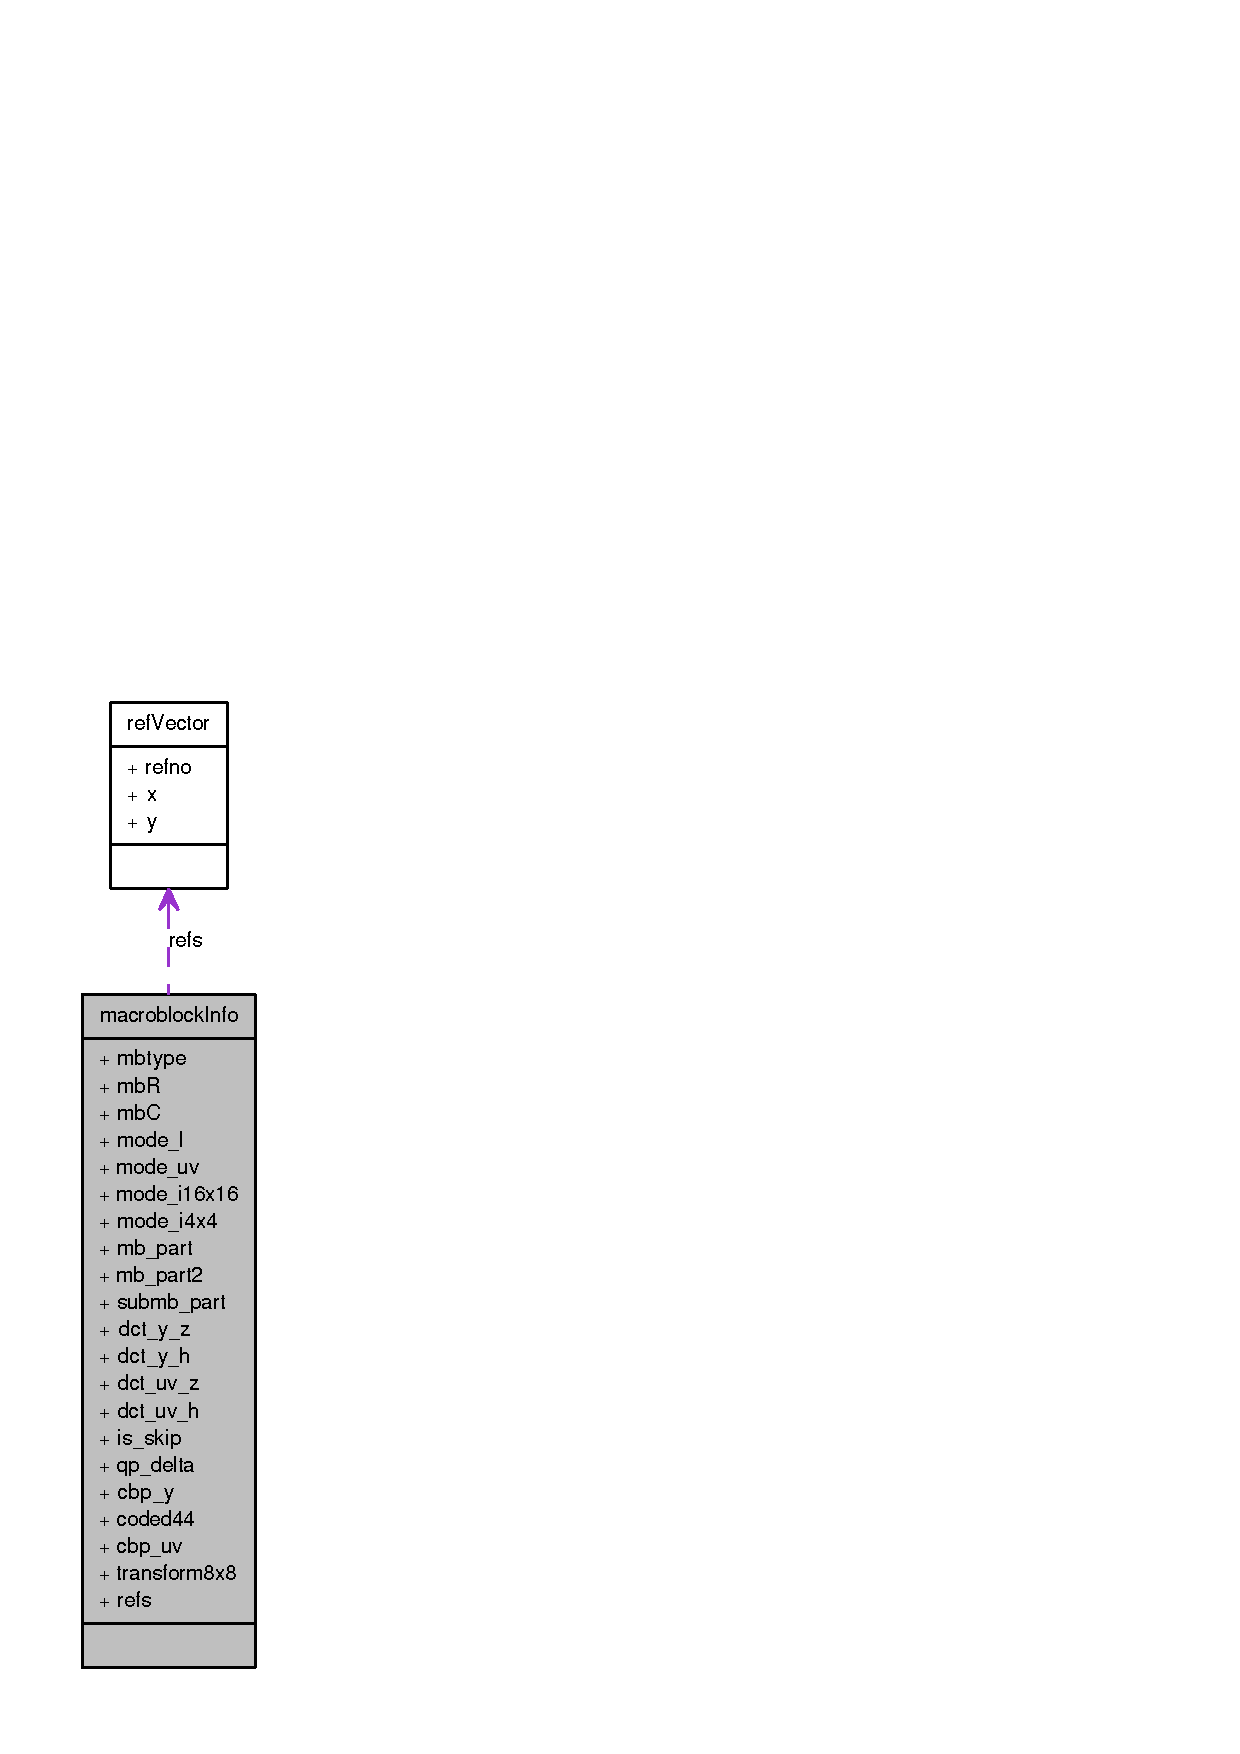
\includegraphics[height=400pt]{structmacroblock_info__coll__graph}
\end{center}
\end{figure}
\subsection*{Public Attributes}
\begin{DoxyCompactItemize}
\item 
int \hyperlink{structmacroblock_info_af09f9c522a04fe712528e6db6a696866}{mbtype}
\item 
\hyperlink{_types_8h_ae615613535a2b2445773922f5d45a861}{int16\_\-t} \hyperlink{structmacroblock_info_ae46d0fbf2f0e11fc965a60845db47065}{mbR}
\item 
\hyperlink{_types_8h_ae615613535a2b2445773922f5d45a861}{int16\_\-t} \hyperlink{structmacroblock_info_ab6270e45676c0f84c1450cf90a84df52}{mbC}
\item 
\hyperlink{_types_8h_a363e4d606232036a6b89060813c45489}{uint8\_\-t} \hyperlink{structmacroblock_info_a6bb816cb458ac9c8f908c3f0464cd8ee}{mode\_\-I}
\item 
\hyperlink{_types_8h_a363e4d606232036a6b89060813c45489}{uint8\_\-t} \hyperlink{structmacroblock_info_a562426f4ab2f9cd93c95cff91faaa0f6}{mode\_\-uv}
\item 
\hyperlink{_types_8h_a363e4d606232036a6b89060813c45489}{uint8\_\-t} \hyperlink{structmacroblock_info_a56fac1ac121007a216cd538adc034a16}{mode\_\-i16x16}
\item 
\hyperlink{_types_8h_a363e4d606232036a6b89060813c45489}{uint8\_\-t} \hyperlink{structmacroblock_info_a088e83914a079456b10a7f6db04dfc46}{mode\_\-i4x4} \mbox{[}16\mbox{]}
\item 
\hyperlink{_types_8h_aaf02e775ead73e138f20f66b2846671d}{int8\_\-t} \hyperlink{structmacroblock_info_aca6689d19574d84352bfddf53f5568e4}{mb\_\-part}
\item 
\hyperlink{_types_8h_aaf02e775ead73e138f20f66b2846671d}{int8\_\-t} \hyperlink{structmacroblock_info_a3ac5fa37b331f43add6a74e56e2ffc8d}{mb\_\-part2}
\item 
\hyperlink{_types_8h_aaf02e775ead73e138f20f66b2846671d}{int8\_\-t} \hyperlink{structmacroblock_info_a55e45fad5c7713d3c68b86f07921d2dc}{submb\_\-part} \mbox{[}4\mbox{]}
\item 
\hyperlink{_types_8h_ae615613535a2b2445773922f5d45a861}{int16\_\-t} \hyperlink{structmacroblock_info_ae8398ee14b29db905e426da03b462417}{dct\_\-y\_\-z} \mbox{[}16\mbox{]}\mbox{[}16\mbox{]}
\item 
\hyperlink{_types_8h_ae615613535a2b2445773922f5d45a861}{int16\_\-t} \hyperlink{structmacroblock_info_a60437cc69d5df6184a6b768ff667a70f}{dct\_\-y\_\-h} \mbox{[}16\mbox{]}
\item 
\hyperlink{_types_8h_ae615613535a2b2445773922f5d45a861}{int16\_\-t} \hyperlink{structmacroblock_info_a01c5c766f5445434369110a34cd1594e}{dct\_\-uv\_\-z} \mbox{[}2\mbox{]}\mbox{[}4\mbox{]}\mbox{[}16\mbox{]}
\item 
\hyperlink{_types_8h_ae615613535a2b2445773922f5d45a861}{int16\_\-t} \hyperlink{structmacroblock_info_a973346c837d8cf284586c33b4a4d478a}{dct\_\-uv\_\-h} \mbox{[}2\mbox{]}\mbox{[}4\mbox{]}
\item 
\hyperlink{_types_8h_ae615613535a2b2445773922f5d45a861}{int16\_\-t} \hyperlink{structmacroblock_info_ad7cf6f2dc254dc14005ab5705bde6349}{is\_\-skip}
\item 
\hyperlink{_types_8h_ae615613535a2b2445773922f5d45a861}{int16\_\-t} \hyperlink{structmacroblock_info_a732ef45ea0429985a3833fc7a93bf9fd}{qp\_\-delta}
\item 
\hyperlink{_types_8h_ae615613535a2b2445773922f5d45a861}{int16\_\-t} \hyperlink{structmacroblock_info_a39296ecdc137fb62501453716a0330ac}{cbp\_\-y}
\item 
\hyperlink{_types_8h_ae615613535a2b2445773922f5d45a861}{int16\_\-t} \hyperlink{structmacroblock_info_a8c2dc78f061142480ef5b2026b8a1dff}{coded44}
\item 
\hyperlink{_types_8h_ae615613535a2b2445773922f5d45a861}{int16\_\-t} \hyperlink{structmacroblock_info_ae4618a11a8f0f396fb05879125bc449a}{cbp\_\-uv}
\item 
\hyperlink{_types_8h_adde6aaee8457bee49c2a92621fe22b79}{uint8} \hyperlink{structmacroblock_info_a0f244dcaf8b80e1f8adc3973e34e0a25}{transform8x8}
\item 
\hyperlink{structref_vector}{refVector} \hyperlink{structmacroblock_info_a8501600ad3ab8d7865c28c8398e900f9}{refs} \mbox{[}4\mbox{]}\mbox{[}4\mbox{]}\mbox{[}2\mbox{]}
\end{DoxyCompactItemize}


\subsection{Member Data Documentation}
\hypertarget{structmacroblock_info_ae4618a11a8f0f396fb05879125bc449a}{
\index{macroblockInfo@{macroblockInfo}!cbp\_\-uv@{cbp\_\-uv}}
\index{cbp\_\-uv@{cbp\_\-uv}!macroblockInfo@{macroblockInfo}}
\subsubsection[{cbp\_\-uv}]{\setlength{\rightskip}{0pt plus 5cm}{\bf int16\_\-t} {\bf macroblockInfo::cbp\_\-uv}}}
\label{structmacroblock_info_ae4618a11a8f0f396fb05879125bc449a}
\hypertarget{structmacroblock_info_a39296ecdc137fb62501453716a0330ac}{
\index{macroblockInfo@{macroblockInfo}!cbp\_\-y@{cbp\_\-y}}
\index{cbp\_\-y@{cbp\_\-y}!macroblockInfo@{macroblockInfo}}
\subsubsection[{cbp\_\-y}]{\setlength{\rightskip}{0pt plus 5cm}{\bf int16\_\-t} {\bf macroblockInfo::cbp\_\-y}}}
\label{structmacroblock_info_a39296ecdc137fb62501453716a0330ac}
\hypertarget{structmacroblock_info_a8c2dc78f061142480ef5b2026b8a1dff}{
\index{macroblockInfo@{macroblockInfo}!coded44@{coded44}}
\index{coded44@{coded44}!macroblockInfo@{macroblockInfo}}
\subsubsection[{coded44}]{\setlength{\rightskip}{0pt plus 5cm}{\bf int16\_\-t} {\bf macroblockInfo::coded44}}}
\label{structmacroblock_info_a8c2dc78f061142480ef5b2026b8a1dff}
\hypertarget{structmacroblock_info_a973346c837d8cf284586c33b4a4d478a}{
\index{macroblockInfo@{macroblockInfo}!dct\_\-uv\_\-h@{dct\_\-uv\_\-h}}
\index{dct\_\-uv\_\-h@{dct\_\-uv\_\-h}!macroblockInfo@{macroblockInfo}}
\subsubsection[{dct\_\-uv\_\-h}]{\setlength{\rightskip}{0pt plus 5cm}{\bf int16\_\-t} {\bf macroblockInfo::dct\_\-uv\_\-h}\mbox{[}2\mbox{]}\mbox{[}4\mbox{]}}}
\label{structmacroblock_info_a973346c837d8cf284586c33b4a4d478a}
\hypertarget{structmacroblock_info_a01c5c766f5445434369110a34cd1594e}{
\index{macroblockInfo@{macroblockInfo}!dct\_\-uv\_\-z@{dct\_\-uv\_\-z}}
\index{dct\_\-uv\_\-z@{dct\_\-uv\_\-z}!macroblockInfo@{macroblockInfo}}
\subsubsection[{dct\_\-uv\_\-z}]{\setlength{\rightskip}{0pt plus 5cm}{\bf int16\_\-t} {\bf macroblockInfo::dct\_\-uv\_\-z}\mbox{[}2\mbox{]}\mbox{[}4\mbox{]}\mbox{[}16\mbox{]}}}
\label{structmacroblock_info_a01c5c766f5445434369110a34cd1594e}
\hypertarget{structmacroblock_info_a60437cc69d5df6184a6b768ff667a70f}{
\index{macroblockInfo@{macroblockInfo}!dct\_\-y\_\-h@{dct\_\-y\_\-h}}
\index{dct\_\-y\_\-h@{dct\_\-y\_\-h}!macroblockInfo@{macroblockInfo}}
\subsubsection[{dct\_\-y\_\-h}]{\setlength{\rightskip}{0pt plus 5cm}{\bf int16\_\-t} {\bf macroblockInfo::dct\_\-y\_\-h}\mbox{[}16\mbox{]}}}
\label{structmacroblock_info_a60437cc69d5df6184a6b768ff667a70f}
\hypertarget{structmacroblock_info_ae8398ee14b29db905e426da03b462417}{
\index{macroblockInfo@{macroblockInfo}!dct\_\-y\_\-z@{dct\_\-y\_\-z}}
\index{dct\_\-y\_\-z@{dct\_\-y\_\-z}!macroblockInfo@{macroblockInfo}}
\subsubsection[{dct\_\-y\_\-z}]{\setlength{\rightskip}{0pt plus 5cm}{\bf int16\_\-t} {\bf macroblockInfo::dct\_\-y\_\-z}\mbox{[}16\mbox{]}\mbox{[}16\mbox{]}}}
\label{structmacroblock_info_ae8398ee14b29db905e426da03b462417}
\hypertarget{structmacroblock_info_ad7cf6f2dc254dc14005ab5705bde6349}{
\index{macroblockInfo@{macroblockInfo}!is\_\-skip@{is\_\-skip}}
\index{is\_\-skip@{is\_\-skip}!macroblockInfo@{macroblockInfo}}
\subsubsection[{is\_\-skip}]{\setlength{\rightskip}{0pt plus 5cm}{\bf int16\_\-t} {\bf macroblockInfo::is\_\-skip}}}
\label{structmacroblock_info_ad7cf6f2dc254dc14005ab5705bde6349}
\hypertarget{structmacroblock_info_aca6689d19574d84352bfddf53f5568e4}{
\index{macroblockInfo@{macroblockInfo}!mb\_\-part@{mb\_\-part}}
\index{mb\_\-part@{mb\_\-part}!macroblockInfo@{macroblockInfo}}
\subsubsection[{mb\_\-part}]{\setlength{\rightskip}{0pt plus 5cm}{\bf int8\_\-t} {\bf macroblockInfo::mb\_\-part}}}
\label{structmacroblock_info_aca6689d19574d84352bfddf53f5568e4}
\hypertarget{structmacroblock_info_a3ac5fa37b331f43add6a74e56e2ffc8d}{
\index{macroblockInfo@{macroblockInfo}!mb\_\-part2@{mb\_\-part2}}
\index{mb\_\-part2@{mb\_\-part2}!macroblockInfo@{macroblockInfo}}
\subsubsection[{mb\_\-part2}]{\setlength{\rightskip}{0pt plus 5cm}{\bf int8\_\-t} {\bf macroblockInfo::mb\_\-part2}}}
\label{structmacroblock_info_a3ac5fa37b331f43add6a74e56e2ffc8d}
\hypertarget{structmacroblock_info_ab6270e45676c0f84c1450cf90a84df52}{
\index{macroblockInfo@{macroblockInfo}!mbC@{mbC}}
\index{mbC@{mbC}!macroblockInfo@{macroblockInfo}}
\subsubsection[{mbC}]{\setlength{\rightskip}{0pt plus 5cm}{\bf int16\_\-t} {\bf macroblockInfo::mbC}}}
\label{structmacroblock_info_ab6270e45676c0f84c1450cf90a84df52}
\hypertarget{structmacroblock_info_ae46d0fbf2f0e11fc965a60845db47065}{
\index{macroblockInfo@{macroblockInfo}!mbR@{mbR}}
\index{mbR@{mbR}!macroblockInfo@{macroblockInfo}}
\subsubsection[{mbR}]{\setlength{\rightskip}{0pt plus 5cm}{\bf int16\_\-t} {\bf macroblockInfo::mbR}}}
\label{structmacroblock_info_ae46d0fbf2f0e11fc965a60845db47065}
\hypertarget{structmacroblock_info_af09f9c522a04fe712528e6db6a696866}{
\index{macroblockInfo@{macroblockInfo}!mbtype@{mbtype}}
\index{mbtype@{mbtype}!macroblockInfo@{macroblockInfo}}
\subsubsection[{mbtype}]{\setlength{\rightskip}{0pt plus 5cm}int {\bf macroblockInfo::mbtype}}}
\label{structmacroblock_info_af09f9c522a04fe712528e6db6a696866}
\hypertarget{structmacroblock_info_a6bb816cb458ac9c8f908c3f0464cd8ee}{
\index{macroblockInfo@{macroblockInfo}!mode\_\-I@{mode\_\-I}}
\index{mode\_\-I@{mode\_\-I}!macroblockInfo@{macroblockInfo}}
\subsubsection[{mode\_\-I}]{\setlength{\rightskip}{0pt plus 5cm}{\bf uint8\_\-t} {\bf macroblockInfo::mode\_\-I}}}
\label{structmacroblock_info_a6bb816cb458ac9c8f908c3f0464cd8ee}
\hypertarget{structmacroblock_info_a56fac1ac121007a216cd538adc034a16}{
\index{macroblockInfo@{macroblockInfo}!mode\_\-i16x16@{mode\_\-i16x16}}
\index{mode\_\-i16x16@{mode\_\-i16x16}!macroblockInfo@{macroblockInfo}}
\subsubsection[{mode\_\-i16x16}]{\setlength{\rightskip}{0pt plus 5cm}{\bf uint8\_\-t} {\bf macroblockInfo::mode\_\-i16x16}}}
\label{structmacroblock_info_a56fac1ac121007a216cd538adc034a16}
\hypertarget{structmacroblock_info_a088e83914a079456b10a7f6db04dfc46}{
\index{macroblockInfo@{macroblockInfo}!mode\_\-i4x4@{mode\_\-i4x4}}
\index{mode\_\-i4x4@{mode\_\-i4x4}!macroblockInfo@{macroblockInfo}}
\subsubsection[{mode\_\-i4x4}]{\setlength{\rightskip}{0pt plus 5cm}{\bf uint8\_\-t} {\bf macroblockInfo::mode\_\-i4x4}\mbox{[}16\mbox{]}}}
\label{structmacroblock_info_a088e83914a079456b10a7f6db04dfc46}
\hypertarget{structmacroblock_info_a562426f4ab2f9cd93c95cff91faaa0f6}{
\index{macroblockInfo@{macroblockInfo}!mode\_\-uv@{mode\_\-uv}}
\index{mode\_\-uv@{mode\_\-uv}!macroblockInfo@{macroblockInfo}}
\subsubsection[{mode\_\-uv}]{\setlength{\rightskip}{0pt plus 5cm}{\bf uint8\_\-t} {\bf macroblockInfo::mode\_\-uv}}}
\label{structmacroblock_info_a562426f4ab2f9cd93c95cff91faaa0f6}
\hypertarget{structmacroblock_info_a732ef45ea0429985a3833fc7a93bf9fd}{
\index{macroblockInfo@{macroblockInfo}!qp\_\-delta@{qp\_\-delta}}
\index{qp\_\-delta@{qp\_\-delta}!macroblockInfo@{macroblockInfo}}
\subsubsection[{qp\_\-delta}]{\setlength{\rightskip}{0pt plus 5cm}{\bf int16\_\-t} {\bf macroblockInfo::qp\_\-delta}}}
\label{structmacroblock_info_a732ef45ea0429985a3833fc7a93bf9fd}
\hypertarget{structmacroblock_info_a8501600ad3ab8d7865c28c8398e900f9}{
\index{macroblockInfo@{macroblockInfo}!refs@{refs}}
\index{refs@{refs}!macroblockInfo@{macroblockInfo}}
\subsubsection[{refs}]{\setlength{\rightskip}{0pt plus 5cm}{\bf refVector} {\bf macroblockInfo::refs}\mbox{[}4\mbox{]}\mbox{[}4\mbox{]}\mbox{[}2\mbox{]}}}
\label{structmacroblock_info_a8501600ad3ab8d7865c28c8398e900f9}
\hypertarget{structmacroblock_info_a55e45fad5c7713d3c68b86f07921d2dc}{
\index{macroblockInfo@{macroblockInfo}!submb\_\-part@{submb\_\-part}}
\index{submb\_\-part@{submb\_\-part}!macroblockInfo@{macroblockInfo}}
\subsubsection[{submb\_\-part}]{\setlength{\rightskip}{0pt plus 5cm}{\bf int8\_\-t} {\bf macroblockInfo::submb\_\-part}\mbox{[}4\mbox{]}}}
\label{structmacroblock_info_a55e45fad5c7713d3c68b86f07921d2dc}
\hypertarget{structmacroblock_info_a0f244dcaf8b80e1f8adc3973e34e0a25}{
\index{macroblockInfo@{macroblockInfo}!transform8x8@{transform8x8}}
\index{transform8x8@{transform8x8}!macroblockInfo@{macroblockInfo}}
\subsubsection[{transform8x8}]{\setlength{\rightskip}{0pt plus 5cm}{\bf uint8} {\bf macroblockInfo::transform8x8}}}
\label{structmacroblock_info_a0f244dcaf8b80e1f8adc3973e34e0a25}


The documentation for this struct was generated from the following file:\begin{DoxyCompactItemize}
\item 
MVCCommonLib/\hyperlink{_types_8h}{Types.h}\end{DoxyCompactItemize}

\hypertarget{class_pair}{
\section{Pair$<$ T1, T2 $>$ Class Template Reference}
\label{class_pair}\index{Pair@{Pair}}
}


{\ttfamily \#include $<$Pair.h$>$}

\subsection*{Public Member Functions}
\begin{DoxyCompactItemize}
\item 
\hyperlink{class_pair_afdbbd798262302838fcf7ce963b8182b}{Pair} ()
\item 
\hyperlink{class_pair_acd296016a9da2ebd34c6e582bf9bc687}{Pair} (T1 \hyperlink{class_pair_a3b0b4ac2336a2228fa2af5ceebe31804}{first}, T2 \hyperlink{class_pair_af56592579c6ce0d7e03bad0fcaa5d93e}{second})
\item 
\hyperlink{class_pair_a2067d5333367a0cbc5a3dc6deffaab33}{Pair} (const \hyperlink{class_pair}{Pair} \&r)
\item 
\hyperlink{class_pair}{Pair} \& \hyperlink{class_pair_ac16244bfa58bf7b3cc2d7824c16ac249}{operator=} (const \hyperlink{class_pair}{Pair} \&r)
\item 
bool \hyperlink{class_pair_aa63d09e321533b938f87de0ebfe86940}{operator$<$} (const \hyperlink{class_pair}{Pair} \&r) const 
\item 
bool \hyperlink{class_pair_a3578a7b13595aade4bb84d7a1948d498}{operator==} (const \hyperlink{class_pair}{Pair} \&r) const 
\end{DoxyCompactItemize}
\subsection*{Public Attributes}
\begin{DoxyCompactItemize}
\item 
T1 \hyperlink{class_pair_a3b0b4ac2336a2228fa2af5ceebe31804}{first}
\item 
T2 \hyperlink{class_pair_af56592579c6ce0d7e03bad0fcaa5d93e}{second}
\end{DoxyCompactItemize}
\subsubsection*{template$<$class T1, class T2$>$ class Pair$<$ T1, T2 $>$}



\subsection{Constructor \& Destructor Documentation}
\hypertarget{class_pair_afdbbd798262302838fcf7ce963b8182b}{
\index{Pair@{Pair}!Pair@{Pair}}
\index{Pair@{Pair}!Pair@{Pair}}
\subsubsection[{Pair}]{\setlength{\rightskip}{0pt plus 5cm}template$<$class T1, class T2$>$ {\bf Pair}$<$ T1, T2 $>$::{\bf Pair} ()\hspace{0.3cm}{\ttfamily  \mbox{[}inline\mbox{]}}}}
\label{class_pair_afdbbd798262302838fcf7ce963b8182b}




\begin{footnotesize}\begin{alltt}
00011                : \hyperlink{class_pair_a3b0b4ac2336a2228fa2af5ceebe31804}{first}(T1()), \hyperlink{class_pair_af56592579c6ce0d7e03bad0fcaa5d93e}{second}(T2())
00012         \{\}
\end{alltt}\end{footnotesize}


\hypertarget{class_pair_acd296016a9da2ebd34c6e582bf9bc687}{
\index{Pair@{Pair}!Pair@{Pair}}
\index{Pair@{Pair}!Pair@{Pair}}
\subsubsection[{Pair}]{\setlength{\rightskip}{0pt plus 5cm}template$<$class T1, class T2$>$ {\bf Pair}$<$ T1, T2 $>$::{\bf Pair} (T1 {\em first}, \/  T2 {\em second})\hspace{0.3cm}{\ttfamily  \mbox{[}inline\mbox{]}}}}
\label{class_pair_acd296016a9da2ebd34c6e582bf9bc687}




\begin{footnotesize}\begin{alltt}
00014                                   : \hyperlink{class_pair_a3b0b4ac2336a2228fa2af5ceebe31804}{first}(\hyperlink{class_pair_a3b0b4ac2336a2228fa2af5ceebe31804}{first}), \hyperlink{class_pair_af56592579c6ce0d7e03bad0fcaa5d93e}{second}(\hyperlink{class_pair_af56592579c6ce0d7e03bad0fcaa5d93e}{second})
00015         \{\}
\end{alltt}\end{footnotesize}


\hypertarget{class_pair_a2067d5333367a0cbc5a3dc6deffaab33}{
\index{Pair@{Pair}!Pair@{Pair}}
\index{Pair@{Pair}!Pair@{Pair}}
\subsubsection[{Pair}]{\setlength{\rightskip}{0pt plus 5cm}template$<$class T1, class T2$>$ {\bf Pair}$<$ T1, T2 $>$::{\bf Pair} (const {\bf Pair}$<$ T1, T2 $>$ \& {\em r})\hspace{0.3cm}{\ttfamily  \mbox{[}inline\mbox{]}}}}
\label{class_pair_a2067d5333367a0cbc5a3dc6deffaab33}




\begin{footnotesize}\begin{alltt}
00017                             : \hyperlink{class_pair_a3b0b4ac2336a2228fa2af5ceebe31804}{first}(r.\hyperlink{class_pair_a3b0b4ac2336a2228fa2af5ceebe31804}{first}), \hyperlink{class_pair_af56592579c6ce0d7e03bad0fcaa5d93e}{second}(r.\hyperlink{class_pair_af56592579c6ce0d7e03bad0fcaa5d93e}{second})
00018         \{\}
\end{alltt}\end{footnotesize}




\subsection{Member Function Documentation}
\hypertarget{class_pair_aa63d09e321533b938f87de0ebfe86940}{
\index{Pair@{Pair}!operator$<$@{operator$<$}}
\index{operator$<$@{operator$<$}!Pair@{Pair}}
\subsubsection[{operator$<$}]{\setlength{\rightskip}{0pt plus 5cm}template$<$class T1, class T2$>$ bool {\bf Pair}$<$ T1, T2 $>$::operator$<$ (const {\bf Pair}$<$ T1, T2 $>$ \& {\em r}) const\hspace{0.3cm}{\ttfamily  \mbox{[}inline\mbox{]}}}}
\label{class_pair_aa63d09e321533b938f87de0ebfe86940}




\begin{footnotesize}\begin{alltt}
00028         \{
00029                 \textcolor{keywordflow}{if} (\hyperlink{class_pair_a3b0b4ac2336a2228fa2af5ceebe31804}{first} < r.\hyperlink{class_pair_a3b0b4ac2336a2228fa2af5ceebe31804}{first})
00030                         \textcolor{keywordflow}{return} \textcolor{keyword}{true};
00031                 \textcolor{keywordflow}{if} (r.\hyperlink{class_pair_a3b0b4ac2336a2228fa2af5ceebe31804}{first} < \hyperlink{class_pair_a3b0b4ac2336a2228fa2af5ceebe31804}{first})
00032                         \textcolor{keywordflow}{return} \textcolor{keyword}{false};
00033                 \textcolor{keywordflow}{return} \hyperlink{class_pair_af56592579c6ce0d7e03bad0fcaa5d93e}{second} < r.\hyperlink{class_pair_af56592579c6ce0d7e03bad0fcaa5d93e}{second};
00034         \}
\end{alltt}\end{footnotesize}


\hypertarget{class_pair_ac16244bfa58bf7b3cc2d7824c16ac249}{
\index{Pair@{Pair}!operator=@{operator=}}
\index{operator=@{operator=}!Pair@{Pair}}
\subsubsection[{operator=}]{\setlength{\rightskip}{0pt plus 5cm}template$<$class T1, class T2$>$ {\bf Pair}\& {\bf Pair}$<$ T1, T2 $>$::operator= (const {\bf Pair}$<$ T1, T2 $>$ \& {\em r})\hspace{0.3cm}{\ttfamily  \mbox{[}inline\mbox{]}}}}
\label{class_pair_ac16244bfa58bf7b3cc2d7824c16ac249}




\begin{footnotesize}\begin{alltt}
00021         \{
00022                 \hyperlink{class_pair_a3b0b4ac2336a2228fa2af5ceebe31804}{first} = r.\hyperlink{class_pair_a3b0b4ac2336a2228fa2af5ceebe31804}{first};
00023                 \hyperlink{class_pair_af56592579c6ce0d7e03bad0fcaa5d93e}{second} = r.\hyperlink{class_pair_af56592579c6ce0d7e03bad0fcaa5d93e}{second};
00024                 \textcolor{keywordflow}{return} *\textcolor{keyword}{this};
00025         \}
\end{alltt}\end{footnotesize}


\hypertarget{class_pair_a3578a7b13595aade4bb84d7a1948d498}{
\index{Pair@{Pair}!operator==@{operator==}}
\index{operator==@{operator==}!Pair@{Pair}}
\subsubsection[{operator==}]{\setlength{\rightskip}{0pt plus 5cm}template$<$class T1, class T2$>$ bool {\bf Pair}$<$ T1, T2 $>$::operator== (const {\bf Pair}$<$ T1, T2 $>$ \& {\em r}) const\hspace{0.3cm}{\ttfamily  \mbox{[}inline\mbox{]}}}}
\label{class_pair_a3578a7b13595aade4bb84d7a1948d498}




\begin{footnotesize}\begin{alltt}
00037         \{
00038                 \textcolor{keywordflow}{return} (\hyperlink{class_pair_a3b0b4ac2336a2228fa2af5ceebe31804}{first}==r.\hyperlink{class_pair_a3b0b4ac2336a2228fa2af5ceebe31804}{first}) && (\hyperlink{class_pair_af56592579c6ce0d7e03bad0fcaa5d93e}{second}==r.\hyperlink{class_pair_af56592579c6ce0d7e03bad0fcaa5d93e}{second});
00039         \}
\end{alltt}\end{footnotesize}




\subsection{Member Data Documentation}
\hypertarget{class_pair_a3b0b4ac2336a2228fa2af5ceebe31804}{
\index{Pair@{Pair}!first@{first}}
\index{first@{first}!Pair@{Pair}}
\subsubsection[{first}]{\setlength{\rightskip}{0pt plus 5cm}template$<$class T1, class T2$>$ T1 {\bf Pair}$<$ T1, T2 $>$::{\bf first}}}
\label{class_pair_a3b0b4ac2336a2228fa2af5ceebe31804}
\hypertarget{class_pair_af56592579c6ce0d7e03bad0fcaa5d93e}{
\index{Pair@{Pair}!second@{second}}
\index{second@{second}!Pair@{Pair}}
\subsubsection[{second}]{\setlength{\rightskip}{0pt plus 5cm}template$<$class T1, class T2$>$ T2 {\bf Pair}$<$ T1, T2 $>$::{\bf second}}}
\label{class_pair_af56592579c6ce0d7e03bad0fcaa5d93e}


The documentation for this class was generated from the following file:\begin{DoxyCompactItemize}
\item 
MVCCommonLib/\hyperlink{_pair_8h}{Pair.h}\end{DoxyCompactItemize}

\hypertarget{struct_p_b_predict_info}{
\section{PBPredictInfo Struct Reference}
\label{struct_p_b_predict_info}\index{PBPredictInfo@{PBPredictInfo}}
}


{\ttfamily \#include $<$Types.h$>$}

\subsection*{Public Attributes}
\begin{DoxyCompactItemize}
\item 
int \hyperlink{struct_p_b_predict_info_a1eda4a8837300bed803d81ada5dfbb30}{myr}
\item 
int \hyperlink{struct_p_b_predict_info_ac46c76693de4dab4a105494d1220dc0a}{myc}
\item 
int \hyperlink{struct_p_b_predict_info_a96c9413deeef7bfcd16237bfef11c8ae}{stride}
\item 
int \hyperlink{struct_p_b_predict_info_a26162322380d1afd96ee0c894f6ee08e}{sizew}
\item 
int \hyperlink{struct_p_b_predict_info_a22f7b2cc9619bf678980e45fc9ef7f1b}{sizeh}
\item 
\hyperlink{_types_8h_a363e4d606232036a6b89060813c45489}{uint8\_\-t} $\ast$ \hyperlink{struct_p_b_predict_info_a7c7d2c72aa539c0e2365b4e04e18a0ca}{pdata\_\-y0} \mbox{[}2\mbox{]}\mbox{[}4\mbox{]}
\item 
\hyperlink{_types_8h_a363e4d606232036a6b89060813c45489}{uint8\_\-t} $\ast$ \hyperlink{struct_p_b_predict_info_aaf07e44714249f4131c030df88bf8169}{pdata\_\-u0} \mbox{[}2\mbox{]}\mbox{[}4\mbox{]}
\item 
\hyperlink{_types_8h_a363e4d606232036a6b89060813c45489}{uint8\_\-t} $\ast$ \hyperlink{struct_p_b_predict_info_a8dc8f424bcb4274ef583207aa9827962}{pdata\_\-v0} \mbox{[}2\mbox{]}\mbox{[}4\mbox{]}
\item 
\hyperlink{_types_8h_a363e4d606232036a6b89060813c45489}{uint8\_\-t} \hyperlink{struct_p_b_predict_info_aaa7f5b9d6def9506a306d9e5fdf0c7f4}{vdata} \mbox{[}24\mbox{]}\mbox{[}24\mbox{]}
\item 
\hyperlink{_types_8h_a363e4d606232036a6b89060813c45489}{uint8\_\-t} \hyperlink{struct_p_b_predict_info_ae10de4e25fedb10d0ea1dbaf3b34c4ac}{vdata\_\-half} \mbox{[}3\mbox{]}\mbox{[}24\mbox{]}\mbox{[}24\mbox{]}
\end{DoxyCompactItemize}


\subsection{Member Data Documentation}
\hypertarget{struct_p_b_predict_info_ac46c76693de4dab4a105494d1220dc0a}{
\index{PBPredictInfo@{PBPredictInfo}!myc@{myc}}
\index{myc@{myc}!PBPredictInfo@{PBPredictInfo}}
\subsubsection[{myc}]{\setlength{\rightskip}{0pt plus 5cm}int {\bf PBPredictInfo::myc}}}
\label{struct_p_b_predict_info_ac46c76693de4dab4a105494d1220dc0a}
\hypertarget{struct_p_b_predict_info_a1eda4a8837300bed803d81ada5dfbb30}{
\index{PBPredictInfo@{PBPredictInfo}!myr@{myr}}
\index{myr@{myr}!PBPredictInfo@{PBPredictInfo}}
\subsubsection[{myr}]{\setlength{\rightskip}{0pt plus 5cm}int {\bf PBPredictInfo::myr}}}
\label{struct_p_b_predict_info_a1eda4a8837300bed803d81ada5dfbb30}
\hypertarget{struct_p_b_predict_info_aaf07e44714249f4131c030df88bf8169}{
\index{PBPredictInfo@{PBPredictInfo}!pdata\_\-u0@{pdata\_\-u0}}
\index{pdata\_\-u0@{pdata\_\-u0}!PBPredictInfo@{PBPredictInfo}}
\subsubsection[{pdata\_\-u0}]{\setlength{\rightskip}{0pt plus 5cm}{\bf uint8\_\-t}$\ast$ {\bf PBPredictInfo::pdata\_\-u0}\mbox{[}2\mbox{]}\mbox{[}4\mbox{]}}}
\label{struct_p_b_predict_info_aaf07e44714249f4131c030df88bf8169}
\hypertarget{struct_p_b_predict_info_a8dc8f424bcb4274ef583207aa9827962}{
\index{PBPredictInfo@{PBPredictInfo}!pdata\_\-v0@{pdata\_\-v0}}
\index{pdata\_\-v0@{pdata\_\-v0}!PBPredictInfo@{PBPredictInfo}}
\subsubsection[{pdata\_\-v0}]{\setlength{\rightskip}{0pt plus 5cm}{\bf uint8\_\-t}$\ast$ {\bf PBPredictInfo::pdata\_\-v0}\mbox{[}2\mbox{]}\mbox{[}4\mbox{]}}}
\label{struct_p_b_predict_info_a8dc8f424bcb4274ef583207aa9827962}
\hypertarget{struct_p_b_predict_info_a7c7d2c72aa539c0e2365b4e04e18a0ca}{
\index{PBPredictInfo@{PBPredictInfo}!pdata\_\-y0@{pdata\_\-y0}}
\index{pdata\_\-y0@{pdata\_\-y0}!PBPredictInfo@{PBPredictInfo}}
\subsubsection[{pdata\_\-y0}]{\setlength{\rightskip}{0pt plus 5cm}{\bf uint8\_\-t}$\ast$ {\bf PBPredictInfo::pdata\_\-y0}\mbox{[}2\mbox{]}\mbox{[}4\mbox{]}}}
\label{struct_p_b_predict_info_a7c7d2c72aa539c0e2365b4e04e18a0ca}
\hypertarget{struct_p_b_predict_info_a22f7b2cc9619bf678980e45fc9ef7f1b}{
\index{PBPredictInfo@{PBPredictInfo}!sizeh@{sizeh}}
\index{sizeh@{sizeh}!PBPredictInfo@{PBPredictInfo}}
\subsubsection[{sizeh}]{\setlength{\rightskip}{0pt plus 5cm}int {\bf PBPredictInfo::sizeh}}}
\label{struct_p_b_predict_info_a22f7b2cc9619bf678980e45fc9ef7f1b}
\hypertarget{struct_p_b_predict_info_a26162322380d1afd96ee0c894f6ee08e}{
\index{PBPredictInfo@{PBPredictInfo}!sizew@{sizew}}
\index{sizew@{sizew}!PBPredictInfo@{PBPredictInfo}}
\subsubsection[{sizew}]{\setlength{\rightskip}{0pt plus 5cm}int {\bf PBPredictInfo::sizew}}}
\label{struct_p_b_predict_info_a26162322380d1afd96ee0c894f6ee08e}
\hypertarget{struct_p_b_predict_info_a96c9413deeef7bfcd16237bfef11c8ae}{
\index{PBPredictInfo@{PBPredictInfo}!stride@{stride}}
\index{stride@{stride}!PBPredictInfo@{PBPredictInfo}}
\subsubsection[{stride}]{\setlength{\rightskip}{0pt plus 5cm}int {\bf PBPredictInfo::stride}}}
\label{struct_p_b_predict_info_a96c9413deeef7bfcd16237bfef11c8ae}
\hypertarget{struct_p_b_predict_info_aaa7f5b9d6def9506a306d9e5fdf0c7f4}{
\index{PBPredictInfo@{PBPredictInfo}!vdata@{vdata}}
\index{vdata@{vdata}!PBPredictInfo@{PBPredictInfo}}
\subsubsection[{vdata}]{\setlength{\rightskip}{0pt plus 5cm}{\bf uint8\_\-t} {\bf PBPredictInfo::vdata}\mbox{[}24\mbox{]}\mbox{[}24\mbox{]}}}
\label{struct_p_b_predict_info_aaa7f5b9d6def9506a306d9e5fdf0c7f4}
\hypertarget{struct_p_b_predict_info_ae10de4e25fedb10d0ea1dbaf3b34c4ac}{
\index{PBPredictInfo@{PBPredictInfo}!vdata\_\-half@{vdata\_\-half}}
\index{vdata\_\-half@{vdata\_\-half}!PBPredictInfo@{PBPredictInfo}}
\subsubsection[{vdata\_\-half}]{\setlength{\rightskip}{0pt plus 5cm}{\bf uint8\_\-t} {\bf PBPredictInfo::vdata\_\-half}\mbox{[}3\mbox{]}\mbox{[}24\mbox{]}\mbox{[}24\mbox{]}}}
\label{struct_p_b_predict_info_ae10de4e25fedb10d0ea1dbaf3b34c4ac}


The documentation for this struct was generated from the following file:\begin{DoxyCompactItemize}
\item 
MVCCommonLib/\hyperlink{_types_8h}{Types.h}\end{DoxyCompactItemize}

\hypertarget{struct_picture_parameters_set}{
\section{PictureParametersSet Struct Reference}
\label{struct_picture_parameters_set}\index{PictureParametersSet@{PictureParametersSet}}
}


{\ttfamily \#include $<$PictureParam.h$>$}

\subsection*{Public Attributes}
\begin{DoxyCompactItemize}
\item 
int \hyperlink{struct_picture_parameters_set_a1c6a508d31929ad84dec0b717ac484a4}{baseQP}
\item 
int \hyperlink{struct_picture_parameters_set_a9611d788502cf2646a1fafd8f1cc7e4f}{pic\_\-order\_\-present\_\-flag}
\item 
int \hyperlink{struct_picture_parameters_set_abc9eb8dcb637bef8a76a7c12380fccf9}{num\_\-ref\_\-idx\_\-l0\_\-active}
\item 
int \hyperlink{struct_picture_parameters_set_afb1dc1e024b6c9263e33d3f1dd233203}{num\_\-ref\_\-idx\_\-l1\_\-active}
\item 
int \hyperlink{struct_picture_parameters_set_a4cd484fee6229fd37fa2bf7519458f3a}{weighted\_\-pred\_\-flag}
\item 
int \hyperlink{struct_picture_parameters_set_a436591953af7e22c28e0e2844acdf9f3}{weighted\_\-bipred\_\-idc}
\end{DoxyCompactItemize}


\subsection{Member Data Documentation}
\hypertarget{struct_picture_parameters_set_a1c6a508d31929ad84dec0b717ac484a4}{
\index{PictureParametersSet@{PictureParametersSet}!baseQP@{baseQP}}
\index{baseQP@{baseQP}!PictureParametersSet@{PictureParametersSet}}
\subsubsection[{baseQP}]{\setlength{\rightskip}{0pt plus 5cm}int {\bf PictureParametersSet::baseQP}}}
\label{struct_picture_parameters_set_a1c6a508d31929ad84dec0b717ac484a4}
\hypertarget{struct_picture_parameters_set_abc9eb8dcb637bef8a76a7c12380fccf9}{
\index{PictureParametersSet@{PictureParametersSet}!num\_\-ref\_\-idx\_\-l0\_\-active@{num\_\-ref\_\-idx\_\-l0\_\-active}}
\index{num\_\-ref\_\-idx\_\-l0\_\-active@{num\_\-ref\_\-idx\_\-l0\_\-active}!PictureParametersSet@{PictureParametersSet}}
\subsubsection[{num\_\-ref\_\-idx\_\-l0\_\-active}]{\setlength{\rightskip}{0pt plus 5cm}int {\bf PictureParametersSet::num\_\-ref\_\-idx\_\-l0\_\-active}}}
\label{struct_picture_parameters_set_abc9eb8dcb637bef8a76a7c12380fccf9}
\hypertarget{struct_picture_parameters_set_afb1dc1e024b6c9263e33d3f1dd233203}{
\index{PictureParametersSet@{PictureParametersSet}!num\_\-ref\_\-idx\_\-l1\_\-active@{num\_\-ref\_\-idx\_\-l1\_\-active}}
\index{num\_\-ref\_\-idx\_\-l1\_\-active@{num\_\-ref\_\-idx\_\-l1\_\-active}!PictureParametersSet@{PictureParametersSet}}
\subsubsection[{num\_\-ref\_\-idx\_\-l1\_\-active}]{\setlength{\rightskip}{0pt plus 5cm}int {\bf PictureParametersSet::num\_\-ref\_\-idx\_\-l1\_\-active}}}
\label{struct_picture_parameters_set_afb1dc1e024b6c9263e33d3f1dd233203}
\hypertarget{struct_picture_parameters_set_a9611d788502cf2646a1fafd8f1cc7e4f}{
\index{PictureParametersSet@{PictureParametersSet}!pic\_\-order\_\-present\_\-flag@{pic\_\-order\_\-present\_\-flag}}
\index{pic\_\-order\_\-present\_\-flag@{pic\_\-order\_\-present\_\-flag}!PictureParametersSet@{PictureParametersSet}}
\subsubsection[{pic\_\-order\_\-present\_\-flag}]{\setlength{\rightskip}{0pt plus 5cm}int {\bf PictureParametersSet::pic\_\-order\_\-present\_\-flag}}}
\label{struct_picture_parameters_set_a9611d788502cf2646a1fafd8f1cc7e4f}
\hypertarget{struct_picture_parameters_set_a436591953af7e22c28e0e2844acdf9f3}{
\index{PictureParametersSet@{PictureParametersSet}!weighted\_\-bipred\_\-idc@{weighted\_\-bipred\_\-idc}}
\index{weighted\_\-bipred\_\-idc@{weighted\_\-bipred\_\-idc}!PictureParametersSet@{PictureParametersSet}}
\subsubsection[{weighted\_\-bipred\_\-idc}]{\setlength{\rightskip}{0pt plus 5cm}int {\bf PictureParametersSet::weighted\_\-bipred\_\-idc}}}
\label{struct_picture_parameters_set_a436591953af7e22c28e0e2844acdf9f3}
\hypertarget{struct_picture_parameters_set_a4cd484fee6229fd37fa2bf7519458f3a}{
\index{PictureParametersSet@{PictureParametersSet}!weighted\_\-pred\_\-flag@{weighted\_\-pred\_\-flag}}
\index{weighted\_\-pred\_\-flag@{weighted\_\-pred\_\-flag}!PictureParametersSet@{PictureParametersSet}}
\subsubsection[{weighted\_\-pred\_\-flag}]{\setlength{\rightskip}{0pt plus 5cm}int {\bf PictureParametersSet::weighted\_\-pred\_\-flag}}}
\label{struct_picture_parameters_set_a4cd484fee6229fd37fa2bf7519458f3a}


The documentation for this struct was generated from the following file:\begin{DoxyCompactItemize}
\item 
MVCCommonLib/Codec/\hyperlink{_picture_param_8h}{PictureParam.h}\end{DoxyCompactItemize}

\hypertarget{structpredict_info}{
\section{predictInfo Struct Reference}
\label{structpredict_info}\index{predictInfo@{predictInfo}}
}


{\ttfamily \#include $<$Types.h$>$}

\subsection*{Public Attributes}
\begin{DoxyCompactItemize}
\item 
\hyperlink{_types_8h_a363e4d606232036a6b89060813c45489}{uint8\_\-t} \hyperlink{structpredict_info_ab44f7aab3b6e76f7be44d5420f5f4407}{top} \mbox{[}32\mbox{]}
\item 
\hyperlink{_types_8h_a363e4d606232036a6b89060813c45489}{uint8\_\-t} \hyperlink{structpredict_info_aaec86d32b8769dabe17f60051a792e19}{left} \mbox{[}16\mbox{]}
\item 
\hyperlink{_types_8h_a363e4d606232036a6b89060813c45489}{uint8\_\-t} \hyperlink{structpredict_info_a2f363beeef9ca2f90a0db2259fc88f7b}{topleft}
\item 
\hyperlink{_types_8h_a363e4d606232036a6b89060813c45489}{uint8\_\-t} \hyperlink{structpredict_info_a4bb62e14becc6e2eeac45bc8d6a66688}{data\_\-u} \mbox{[}17\mbox{]}
\item 
\hyperlink{_types_8h_a363e4d606232036a6b89060813c45489}{uint8\_\-t} \hyperlink{structpredict_info_ad302972bab20c3c3c87ce4a25efd17a3}{data\_\-v} \mbox{[}17\mbox{]}
\item 
\hyperlink{_types_8h_a363e4d606232036a6b89060813c45489}{uint8\_\-t} \hyperlink{structpredict_info_abe5b70fdeb86bc2d99d9c3e65250fa8e}{hasLeft}
\item 
\hyperlink{_types_8h_a363e4d606232036a6b89060813c45489}{uint8\_\-t} \hyperlink{structpredict_info_a63e51107c5058064b6e8bc3fd6a08b46}{hasTop}
\end{DoxyCompactItemize}


\subsection{Member Data Documentation}
\hypertarget{structpredict_info_a4bb62e14becc6e2eeac45bc8d6a66688}{
\index{predictInfo@{predictInfo}!data\_\-u@{data\_\-u}}
\index{data\_\-u@{data\_\-u}!predictInfo@{predictInfo}}
\subsubsection[{data\_\-u}]{\setlength{\rightskip}{0pt plus 5cm}{\bf uint8\_\-t} {\bf predictInfo::data\_\-u}\mbox{[}17\mbox{]}}}
\label{structpredict_info_a4bb62e14becc6e2eeac45bc8d6a66688}
\hypertarget{structpredict_info_ad302972bab20c3c3c87ce4a25efd17a3}{
\index{predictInfo@{predictInfo}!data\_\-v@{data\_\-v}}
\index{data\_\-v@{data\_\-v}!predictInfo@{predictInfo}}
\subsubsection[{data\_\-v}]{\setlength{\rightskip}{0pt plus 5cm}{\bf uint8\_\-t} {\bf predictInfo::data\_\-v}\mbox{[}17\mbox{]}}}
\label{structpredict_info_ad302972bab20c3c3c87ce4a25efd17a3}
\hypertarget{structpredict_info_abe5b70fdeb86bc2d99d9c3e65250fa8e}{
\index{predictInfo@{predictInfo}!hasLeft@{hasLeft}}
\index{hasLeft@{hasLeft}!predictInfo@{predictInfo}}
\subsubsection[{hasLeft}]{\setlength{\rightskip}{0pt plus 5cm}{\bf uint8\_\-t} {\bf predictInfo::hasLeft}}}
\label{structpredict_info_abe5b70fdeb86bc2d99d9c3e65250fa8e}
\hypertarget{structpredict_info_a63e51107c5058064b6e8bc3fd6a08b46}{
\index{predictInfo@{predictInfo}!hasTop@{hasTop}}
\index{hasTop@{hasTop}!predictInfo@{predictInfo}}
\subsubsection[{hasTop}]{\setlength{\rightskip}{0pt plus 5cm}{\bf uint8\_\-t} {\bf predictInfo::hasTop}}}
\label{structpredict_info_a63e51107c5058064b6e8bc3fd6a08b46}
\hypertarget{structpredict_info_aaec86d32b8769dabe17f60051a792e19}{
\index{predictInfo@{predictInfo}!left@{left}}
\index{left@{left}!predictInfo@{predictInfo}}
\subsubsection[{left}]{\setlength{\rightskip}{0pt plus 5cm}{\bf uint8\_\-t} {\bf predictInfo::left}\mbox{[}16\mbox{]}}}
\label{structpredict_info_aaec86d32b8769dabe17f60051a792e19}
\hypertarget{structpredict_info_ab44f7aab3b6e76f7be44d5420f5f4407}{
\index{predictInfo@{predictInfo}!top@{top}}
\index{top@{top}!predictInfo@{predictInfo}}
\subsubsection[{top}]{\setlength{\rightskip}{0pt plus 5cm}{\bf uint8\_\-t} {\bf predictInfo::top}\mbox{[}32\mbox{]}}}
\label{structpredict_info_ab44f7aab3b6e76f7be44d5420f5f4407}
\hypertarget{structpredict_info_a2f363beeef9ca2f90a0db2259fc88f7b}{
\index{predictInfo@{predictInfo}!topleft@{topleft}}
\index{topleft@{topleft}!predictInfo@{predictInfo}}
\subsubsection[{topleft}]{\setlength{\rightskip}{0pt plus 5cm}{\bf uint8\_\-t} {\bf predictInfo::topleft}}}
\label{structpredict_info_a2f363beeef9ca2f90a0db2259fc88f7b}


The documentation for this struct was generated from the following file:\begin{DoxyCompactItemize}
\item 
MVCCommonLib/\hyperlink{_types_8h}{Types.h}\end{DoxyCompactItemize}

\hypertarget{class_raw_data}{
\section{RawData Class Reference}
\label{class_raw_data}\index{RawData@{RawData}}
}


{\ttfamily \#include $<$RawData.h$>$}



Collaboration diagram for RawData:\nopagebreak
\begin{figure}[H]
\begin{center}
\leavevmode
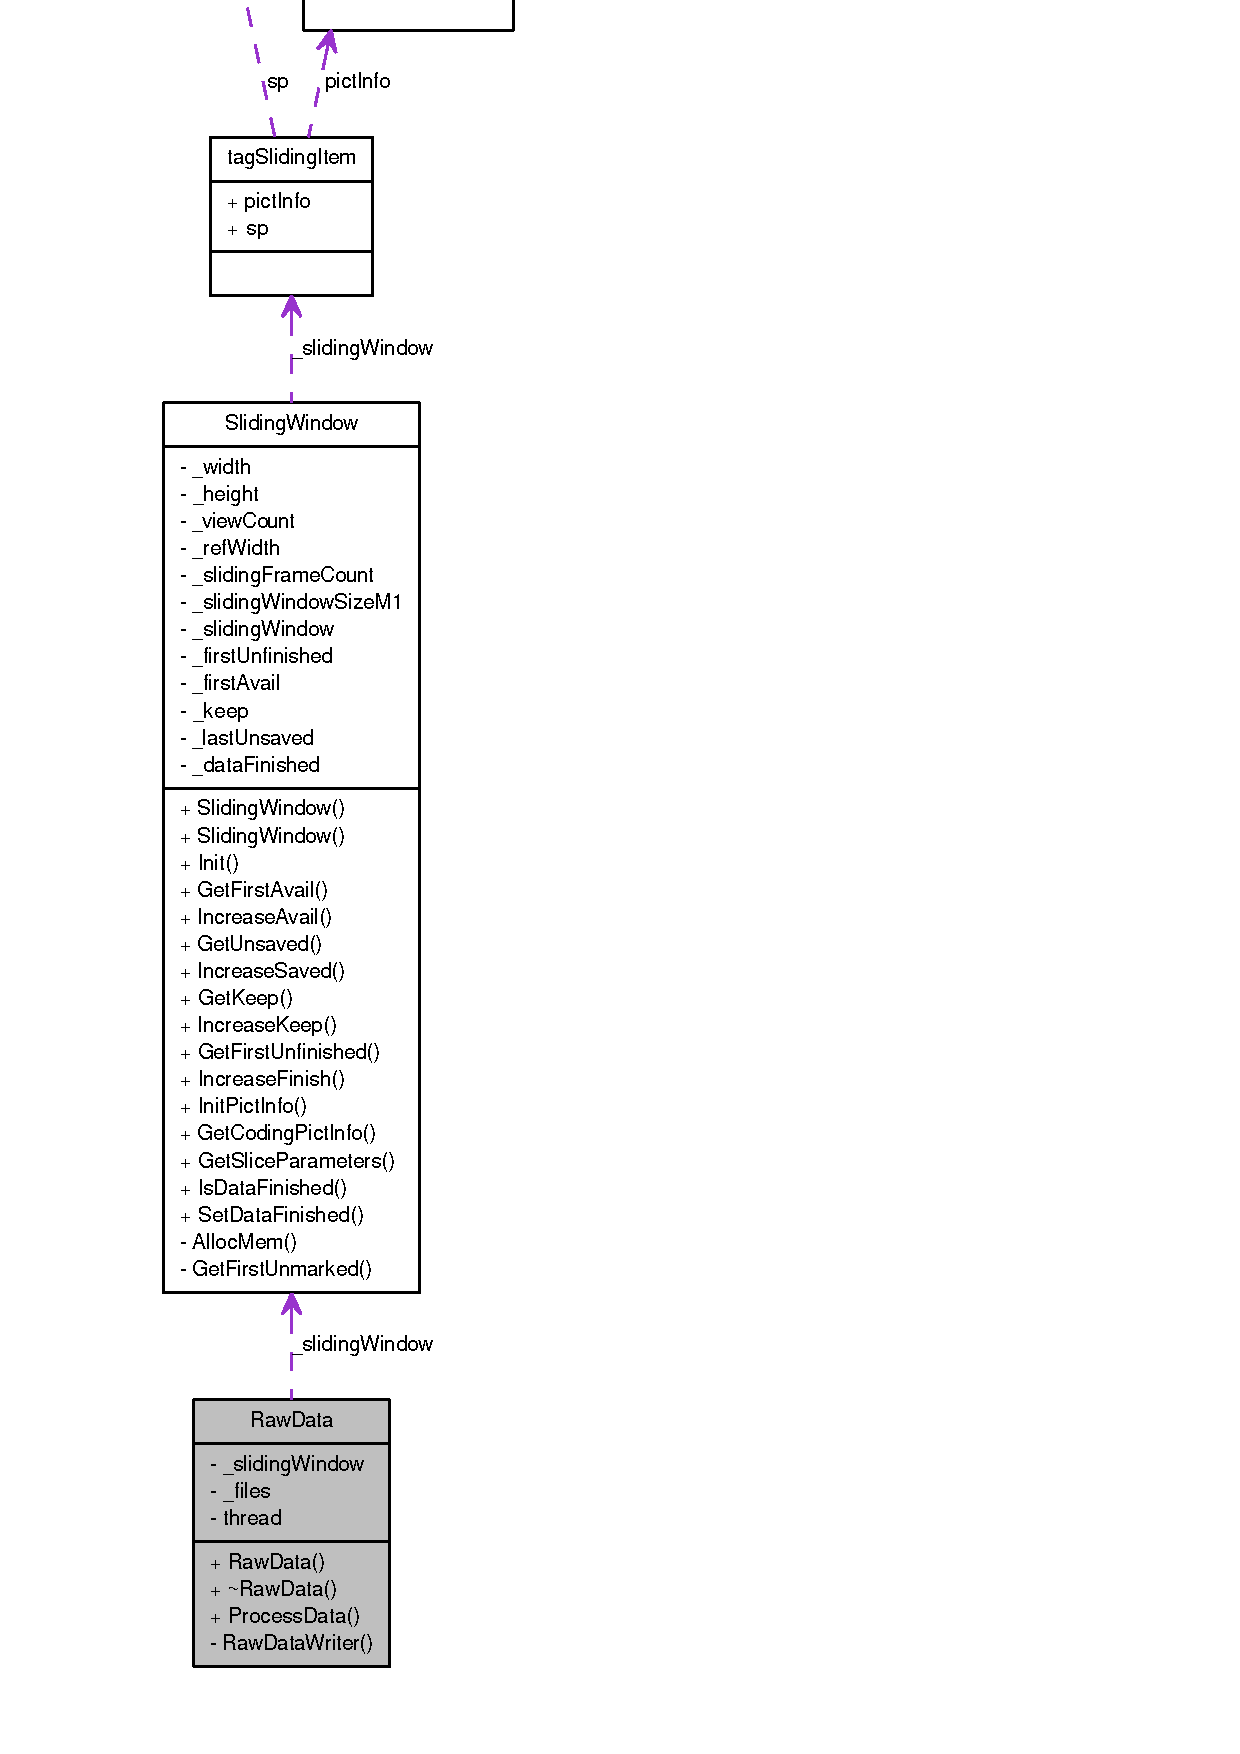
\includegraphics[height=400pt]{class_raw_data__coll__graph}
\end{center}
\end{figure}
\subsection*{Public Member Functions}
\begin{DoxyCompactItemize}
\item 
\hyperlink{class_raw_data_a9a8f2f3170c5574096ea14611f38aca8}{RawData} (\hyperlink{class_sliding_window}{SlidingWindow} $\ast$slidingWindow, const char $\ast$fileNames)
\item 
\hyperlink{class_raw_data_a214d10a81d07c892cb7b35653772e4e4}{$\sim$RawData} ()
\item 
void \hyperlink{class_raw_data_ac1edea5cb8ba51fd52541b415ba36ec2}{ProcessData} ()
\end{DoxyCompactItemize}


\subsection{Constructor \& Destructor Documentation}
\hypertarget{class_raw_data_a9a8f2f3170c5574096ea14611f38aca8}{
\index{RawData@{RawData}!RawData@{RawData}}
\index{RawData@{RawData}!RawData@{RawData}}
\subsubsection[{RawData}]{\setlength{\rightskip}{0pt plus 5cm}RawData::RawData ({\bf SlidingWindow} $\ast$ {\em slidingWindow}, \/  const char $\ast$ {\em fileNames})\hspace{0.3cm}{\ttfamily  \mbox{[}inline\mbox{]}}}}
\label{class_raw_data_a9a8f2f3170c5574096ea14611f38aca8}




\begin{footnotesize}\begin{alltt}
00029                                                                      : \_slidingWi
      ndow(slidingWindow)
00030         \{
00031                 \textcolor{keywordtype}{int} viewCount = \hyperlink{class_codec_info_ad439fd8062a03d868dfe9c9b615b747e}{CodecInfo::GetInstance}().\hyperlink{class_codec_info_aee785011cec77ff3c0c646b498fe1e7d}{sps}.\hyperlink{struct_sequence_parameters_set_af32c7819f630856ccd99aaf78e8f656c}{viewCount};
00032                 \textcolor{keywordtype}{char} fileName[128];
00033                 \_files = \textcolor{keyword}{new} FILE*[viewCount];
00034                 \textcolor{keywordflow}{for} (\textcolor{keywordtype}{int} i = 0; i < viewCount; ++i)
00035                 \{
00036                         sprintf(fileName, fileNames, i);
00037                         \_files[i] = fopen(fileName, \textcolor{stringliteral}{"wb"});
00038                         \hyperlink{_debug_8h_a101586fab2b90a8adffe50a3550e235d}{ASSERT}(\_files[i]);
00039                 \}
00040                 thread = MVCCreateMasterThread(RawDataWriter, \textcolor{keyword}{this});
00041         \}
\end{alltt}\end{footnotesize}




Here is the call graph for this function:\nopagebreak
\begin{figure}[H]
\begin{center}
\leavevmode
\includegraphics[width=222pt]{class_raw_data_a9a8f2f3170c5574096ea14611f38aca8_cgraph}
\end{center}
\end{figure}


\hypertarget{class_raw_data_a214d10a81d07c892cb7b35653772e4e4}{
\index{RawData@{RawData}!$\sim$RawData@{$\sim$RawData}}
\index{$\sim$RawData@{$\sim$RawData}!RawData@{RawData}}
\subsubsection[{$\sim$RawData}]{\setlength{\rightskip}{0pt plus 5cm}RawData::$\sim$RawData ()\hspace{0.3cm}{\ttfamily  \mbox{[}inline\mbox{]}}}}
\label{class_raw_data_a214d10a81d07c892cb7b35653772e4e4}




\begin{footnotesize}\begin{alltt}
00044         \{
00045                 \textcolor{keywordtype}{int} viewCount = \hyperlink{class_codec_info_ad439fd8062a03d868dfe9c9b615b747e}{CodecInfo::GetInstance}().\hyperlink{class_codec_info_aee785011cec77ff3c0c646b498fe1e7d}{sps}.\hyperlink{struct_sequence_parameters_set_af32c7819f630856ccd99aaf78e8f656c}{viewCount};
00046                 MVCWaitMasterThread(thread);
00047                 \textcolor{keywordflow}{for} (\textcolor{keywordtype}{int} i = 0; i < viewCount; ++i)
00048                         fclose(\_files[i]);
00049         \}
\end{alltt}\end{footnotesize}




Here is the call graph for this function:\nopagebreak
\begin{figure}[H]
\begin{center}
\leavevmode
\includegraphics[width=225pt]{class_raw_data_a214d10a81d07c892cb7b35653772e4e4_cgraph}
\end{center}
\end{figure}




\subsection{Member Function Documentation}
\hypertarget{class_raw_data_ac1edea5cb8ba51fd52541b415ba36ec2}{
\index{RawData@{RawData}!ProcessData@{ProcessData}}
\index{ProcessData@{ProcessData}!RawData@{RawData}}
\subsubsection[{ProcessData}]{\setlength{\rightskip}{0pt plus 5cm}void RawData::ProcessData ()\hspace{0.3cm}{\ttfamily  \mbox{[}inline\mbox{]}}}}
\label{class_raw_data_ac1edea5cb8ba51fd52541b415ba36ec2}




\begin{footnotesize}\begin{alltt}
00052         \{
00053                 \textcolor{keywordtype}{int} viewCount = \hyperlink{class_codec_info_ad439fd8062a03d868dfe9c9b615b747e}{CodecInfo::GetInstance}().\hyperlink{class_codec_info_aee785011cec77ff3c0c646b498fe1e7d}{sps}.\hyperlink{struct_sequence_parameters_set_af32c7819f630856ccd99aaf78e8f656c}{viewCount};
00054                 \textcolor{keywordtype}{int} timeId = 0;
00055                 \textcolor{keywordflow}{while} (!\_slidingWindow->\hyperlink{class_sliding_window_afd67521d283b68f9fbc769ee9c0ba4b4}{IsDataFinished}() || \_slidingWindow->
      \hyperlink{class_sliding_window_a3df64e20282ce10a45c4c3f3011e536d}{GetUnsaved}()<\_slidingWindow->\hyperlink{class_sliding_window_a2128091c76b407cd0e244759ba5a2846}{GetFirstAvail}())
00056                 \{
00057                         \textcolor{keywordflow}{while} (timeId >= \_slidingWindow->\hyperlink{class_sliding_window_a2128091c76b407cd0e244759ba5a2846}{GetFirstAvail}())
00058                                 Sleep(10);
00059                         \textcolor{keywordflow}{for} (\textcolor{keywordtype}{int} i = 0; i < viewCount; ++i)
00060                         \{
00061                                 \hyperlink{struct_coding_pict_info}{CodingPictInfo} *cpi = \_slidingWindow->
      \hyperlink{class_sliding_window_ac50874323a2aaa4ef76fab47f80c9f92}{GetCodingPictInfo}(timeId, i);
00062                                 \textcolor{keywordflow}{while} (!(cpi->\hyperlink{struct_coding_pict_info_a41498e5ba764405481005e6569d7f728}{pictStatus}&\hyperlink{_picture_info_8h_a170d5962358e97425e08d5646653494b}{PICT_STATUS_FINISHED}))
00063                                         Sleep(2);
00064                                 \textcolor{comment}{//printf("Writing %d %d\(\backslash\)n", timeId, i);}
00065                                 \textcolor{keywordtype}{int} size = cpi->\hyperlink{struct_coding_pict_info_afeeb373571d44e64d473524e6127f3f7}{Size_Width}*cpi->\hyperlink{struct_coding_pict_info_aa6352dc53234c55d1a0c252c5b8d6141}{Size_Height};
00066                                 fwrite(cpi->\hyperlink{struct_coding_pict_info_a62aee8cc8c9cac725d4f44a19ddc8c2b}{lumaStart}, size, 1, \_files[i]);
00067                                 fwrite(cpi->\hyperlink{struct_coding_pict_info_a103a3180ba57db0bd984a53f0668b70b}{chromaUStart}, size>>2, 1, \_files[i]);
      
00068                                 fwrite(cpi->\hyperlink{struct_coding_pict_info_a7be3395b2a1e7f4b384421c2490dcfdc}{chromaVStart}, size>>2, 1, \_files[i]);
      
00069                                 cpi->\hyperlink{struct_coding_pict_info_a41498e5ba764405481005e6569d7f728}{pictStatus} |= \hyperlink{_picture_info_8h_a81f2be9d3984eb16fa6f3b7daf46466f}{PICT_STATUS_SAVED};
00070                         \}
00071                         ++timeId;
00072                         \textcolor{comment}{//\_slidingWindow->IncreaseSaved();}
00073                         \textcolor{comment}{//printf("TIMEID=%d, UNSAVED=%d\(\backslash\)n", timeId, \_slidingWindo
      w->GetUnsaved());}
00074                 \}
00075         \}
\end{alltt}\end{footnotesize}




Here is the call graph for this function:\nopagebreak
\begin{figure}[H]
\begin{center}
\leavevmode
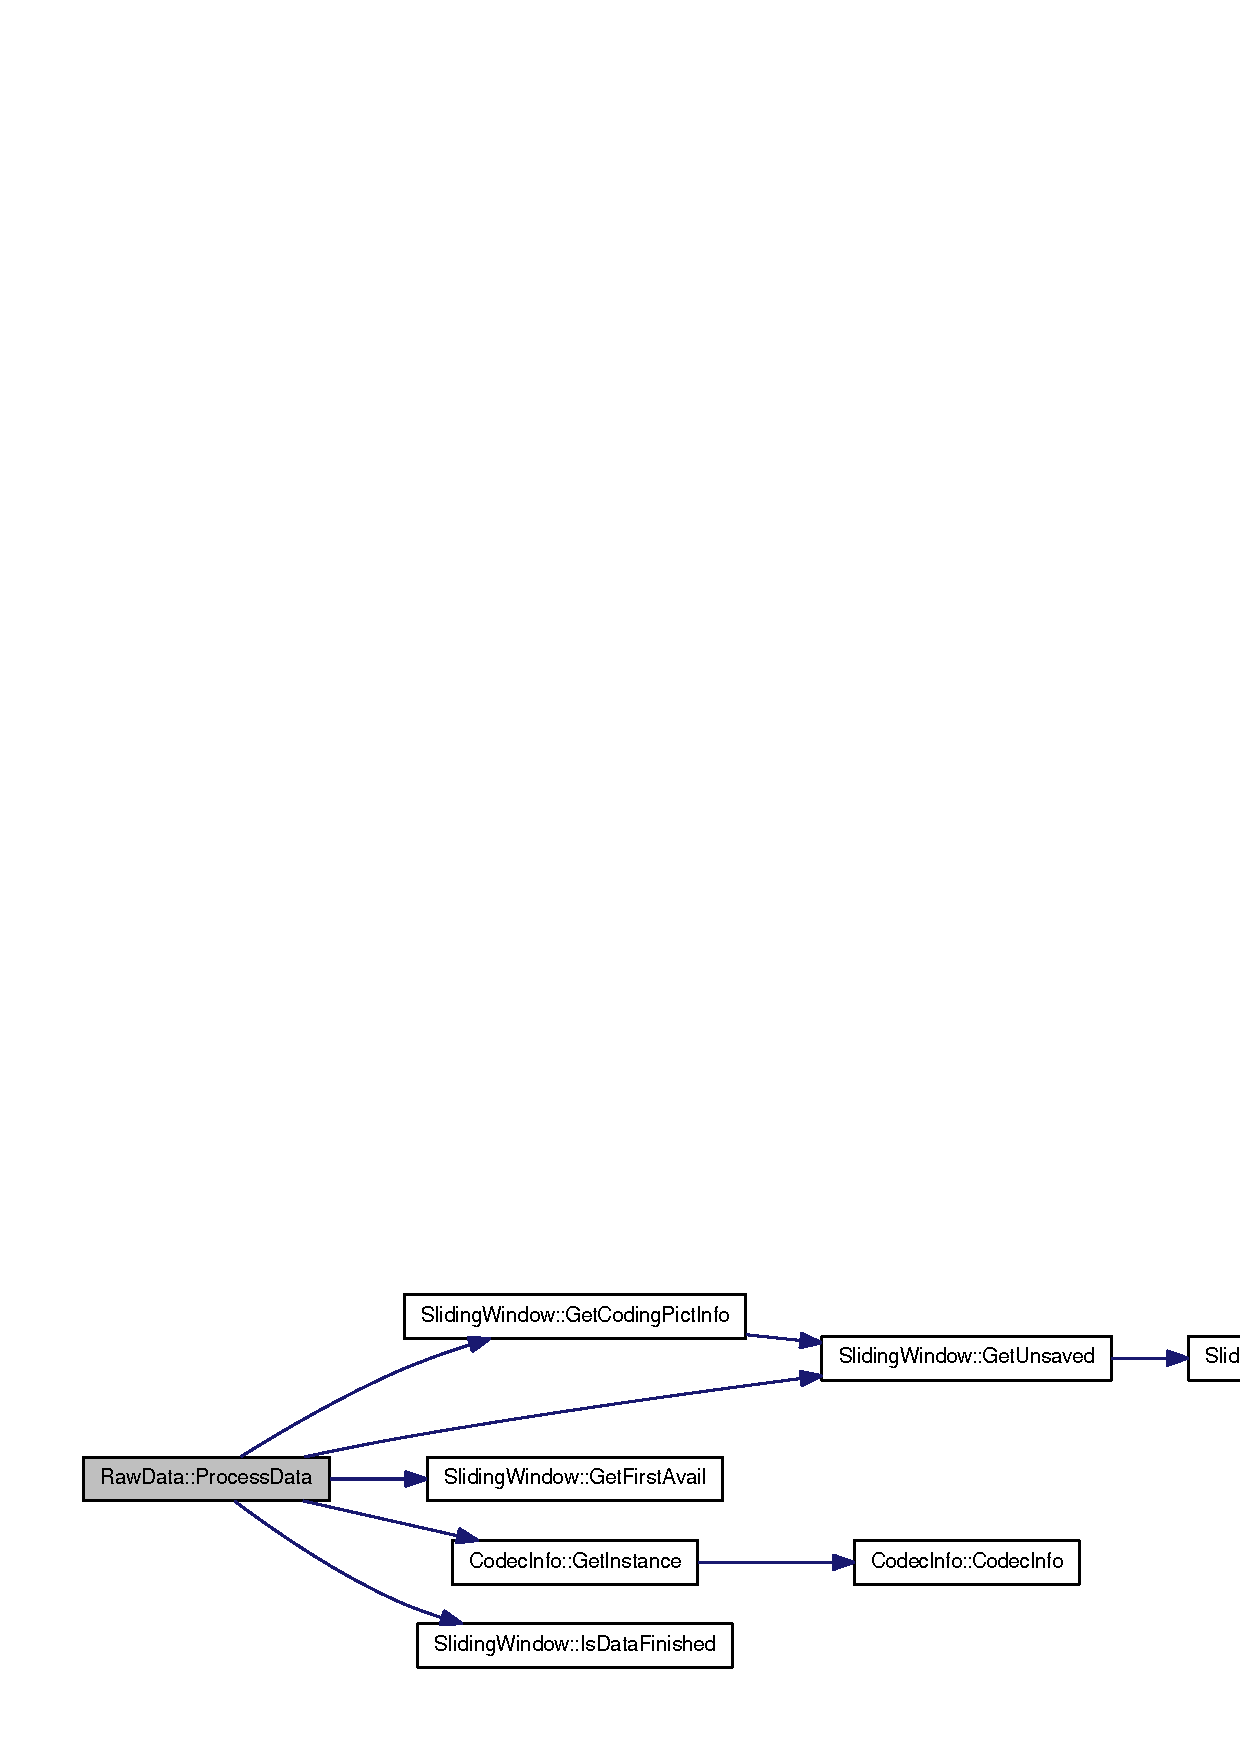
\includegraphics[width=420pt]{class_raw_data_ac1edea5cb8ba51fd52541b415ba36ec2_cgraph}
\end{center}
\end{figure}




The documentation for this class was generated from the following file:\begin{DoxyCompactItemize}
\item 
MVCDecoder/\hyperlink{_raw_data_8h}{RawData.h}\end{DoxyCompactItemize}

\hypertarget{structref_vector}{
\section{refVector Struct Reference}
\label{structref_vector}\index{refVector@{refVector}}
}


{\ttfamily \#include $<$Types.h$>$}

\subsection*{Public Attributes}
\begin{DoxyCompactItemize}
\item 
\hyperlink{_types_8h_aaf02e775ead73e138f20f66b2846671d}{int8\_\-t} \hyperlink{structref_vector_a87a1d38b9e235b983b82abd3a0eb47ab}{refno}
\item 
\hyperlink{_types_8h_ae615613535a2b2445773922f5d45a861}{int16\_\-t} \hyperlink{structref_vector_adeb9dca3f08b25112b9f6bccb5002f48}{x}
\item 
\hyperlink{_types_8h_ae615613535a2b2445773922f5d45a861}{int16\_\-t} \hyperlink{structref_vector_a899825821ce74c5622ea369e32dcf67c}{y}
\end{DoxyCompactItemize}


\subsection{Member Data Documentation}
\hypertarget{structref_vector_a87a1d38b9e235b983b82abd3a0eb47ab}{
\index{refVector@{refVector}!refno@{refno}}
\index{refno@{refno}!refVector@{refVector}}
\subsubsection[{refno}]{\setlength{\rightskip}{0pt plus 5cm}{\bf int8\_\-t} {\bf refVector::refno}}}
\label{structref_vector_a87a1d38b9e235b983b82abd3a0eb47ab}
\hypertarget{structref_vector_adeb9dca3f08b25112b9f6bccb5002f48}{
\index{refVector@{refVector}!x@{x}}
\index{x@{x}!refVector@{refVector}}
\subsubsection[{x}]{\setlength{\rightskip}{0pt plus 5cm}{\bf int16\_\-t} {\bf refVector::x}}}
\label{structref_vector_adeb9dca3f08b25112b9f6bccb5002f48}
\hypertarget{structref_vector_a899825821ce74c5622ea369e32dcf67c}{
\index{refVector@{refVector}!y@{y}}
\index{y@{y}!refVector@{refVector}}
\subsubsection[{y}]{\setlength{\rightskip}{0pt plus 5cm}{\bf int16\_\-t} {\bf refVector::y}}}
\label{structref_vector_a899825821ce74c5622ea369e32dcf67c}


The documentation for this struct was generated from the following file:\begin{DoxyCompactItemize}
\item 
MVCCommonLib/\hyperlink{_types_8h}{Types.h}\end{DoxyCompactItemize}

\hypertarget{struct_sequence_parameters_set}{
\section{SequenceParametersSet Struct Reference}
\label{struct_sequence_parameters_set}\index{SequenceParametersSet@{SequenceParametersSet}}
}


{\ttfamily \#include $<$SequenceParam.h$>$}



Collaboration diagram for SequenceParametersSet:\nopagebreak
\begin{figure}[H]
\begin{center}
\leavevmode
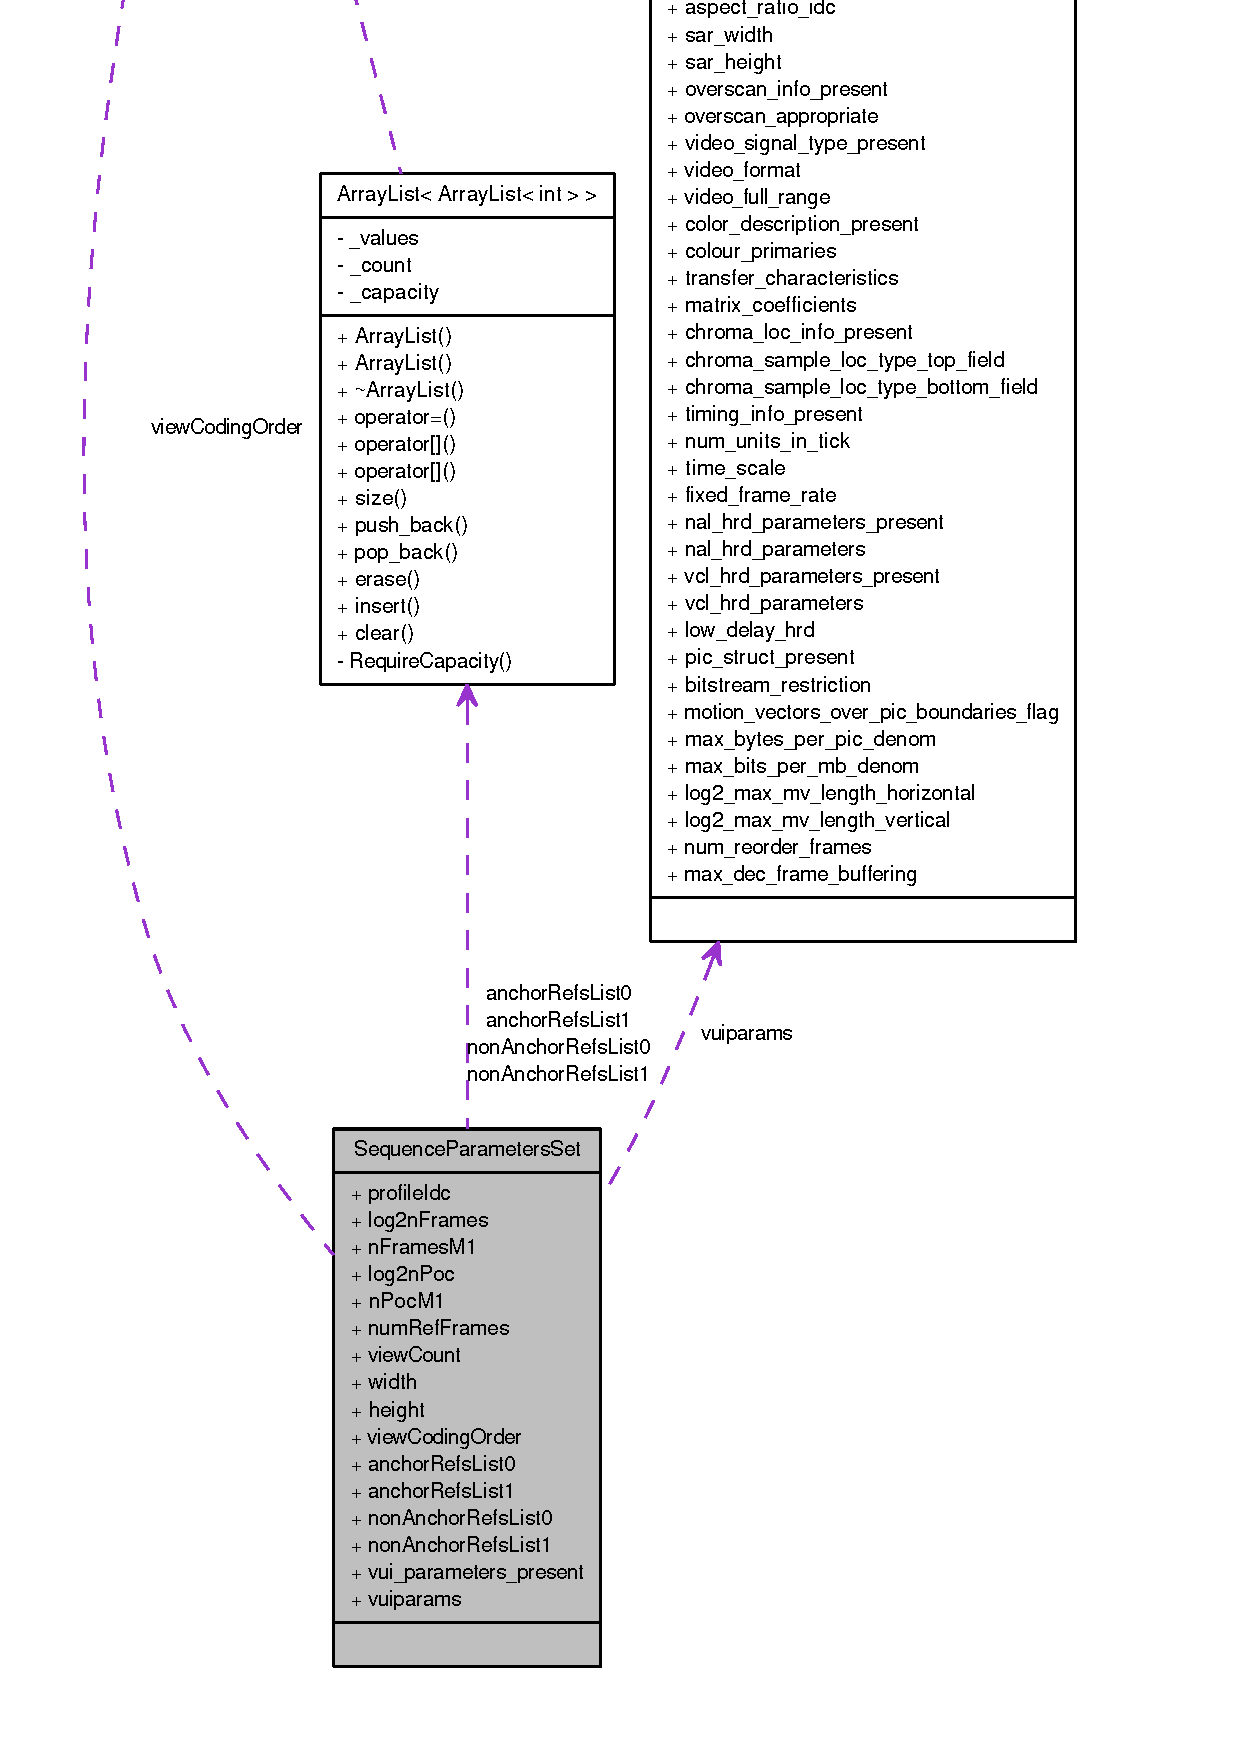
\includegraphics[width=400pt]{struct_sequence_parameters_set__coll__graph}
\end{center}
\end{figure}
\subsection*{Public Attributes}
\begin{DoxyCompactItemize}
\item 
int \hyperlink{struct_sequence_parameters_set_a53070cb0140d170507760e8422f2ef74}{profileIdc}
\item 
int \hyperlink{struct_sequence_parameters_set_ac5f0d82a961acfe4f966e7c35aa37339}{log2nFrames}
\item 
int \hyperlink{struct_sequence_parameters_set_afedac9d01de6ec718715ab45c63ee999}{nFramesM1}
\item 
int \hyperlink{struct_sequence_parameters_set_aff653fc637f7290b7edbaf1cfeacd6ca}{log2nPoc}
\item 
int \hyperlink{struct_sequence_parameters_set_a786d1401a47490d15c7f1512e21994ce}{nPocM1}
\item 
int \hyperlink{struct_sequence_parameters_set_a8404973d25f8601dd012299638361f03}{numRefFrames}
\item 
int \hyperlink{struct_sequence_parameters_set_af32c7819f630856ccd99aaf78e8f656c}{viewCount}
\item 
int \hyperlink{struct_sequence_parameters_set_a72286e512a40a01670e2519b3971cee2}{width}
\item 
int \hyperlink{struct_sequence_parameters_set_ab3b7bd818f9a0d1456d92496473a42eb}{height}
\item 
\hyperlink{class_array_list}{ArrayList}$<$ int $>$ \hyperlink{struct_sequence_parameters_set_a082e13208bc0afd9377676e156e750b4}{viewCodingOrder}
\item 
\hyperlink{class_array_list}{ArrayList}$<$ \hyperlink{class_array_list}{ArrayList}$<$ int $>$ $>$ \hyperlink{struct_sequence_parameters_set_ae9b6a7d85da9fec255cca59c3d750ecd}{anchorRefsList0}
\item 
\hyperlink{class_array_list}{ArrayList}$<$ \hyperlink{class_array_list}{ArrayList}$<$ int $>$ $>$ \hyperlink{struct_sequence_parameters_set_a7b865f89c34428785081c3c4acadc965}{anchorRefsList1}
\item 
\hyperlink{class_array_list}{ArrayList}$<$ \hyperlink{class_array_list}{ArrayList}$<$ int $>$ $>$ \hyperlink{struct_sequence_parameters_set_ab9b078b23e746ef60f7697896b963b93}{nonAnchorRefsList0}
\item 
\hyperlink{class_array_list}{ArrayList}$<$ \hyperlink{class_array_list}{ArrayList}$<$ int $>$ $>$ \hyperlink{struct_sequence_parameters_set_a68b7ffb23b151c53312798f7ab79a67a}{nonAnchorRefsList1}
\item 
bool \hyperlink{struct_sequence_parameters_set_a557345c281f445eb71cbcd5d72a9aed0}{vui\_\-parameters\_\-present}
\item 
\hyperlink{structvui__parameters}{vui\_\-parameters} \hyperlink{struct_sequence_parameters_set_ac473de5b97f08fefdbe39fe9c2c2c846}{vuiparams}
\end{DoxyCompactItemize}


\subsection{Member Data Documentation}
\hypertarget{struct_sequence_parameters_set_ae9b6a7d85da9fec255cca59c3d750ecd}{
\index{SequenceParametersSet@{SequenceParametersSet}!anchorRefsList0@{anchorRefsList0}}
\index{anchorRefsList0@{anchorRefsList0}!SequenceParametersSet@{SequenceParametersSet}}
\subsubsection[{anchorRefsList0}]{\setlength{\rightskip}{0pt plus 5cm}{\bf ArrayList}$<${\bf ArrayList}$<$int$>$ $>$ {\bf SequenceParametersSet::anchorRefsList0}}}
\label{struct_sequence_parameters_set_ae9b6a7d85da9fec255cca59c3d750ecd}
\hypertarget{struct_sequence_parameters_set_a7b865f89c34428785081c3c4acadc965}{
\index{SequenceParametersSet@{SequenceParametersSet}!anchorRefsList1@{anchorRefsList1}}
\index{anchorRefsList1@{anchorRefsList1}!SequenceParametersSet@{SequenceParametersSet}}
\subsubsection[{anchorRefsList1}]{\setlength{\rightskip}{0pt plus 5cm}{\bf ArrayList}$<${\bf ArrayList}$<$int$>$ $>$ {\bf SequenceParametersSet::anchorRefsList1}}}
\label{struct_sequence_parameters_set_a7b865f89c34428785081c3c4acadc965}
\hypertarget{struct_sequence_parameters_set_ab3b7bd818f9a0d1456d92496473a42eb}{
\index{SequenceParametersSet@{SequenceParametersSet}!height@{height}}
\index{height@{height}!SequenceParametersSet@{SequenceParametersSet}}
\subsubsection[{height}]{\setlength{\rightskip}{0pt plus 5cm}int {\bf SequenceParametersSet::height}}}
\label{struct_sequence_parameters_set_ab3b7bd818f9a0d1456d92496473a42eb}
\hypertarget{struct_sequence_parameters_set_ac5f0d82a961acfe4f966e7c35aa37339}{
\index{SequenceParametersSet@{SequenceParametersSet}!log2nFrames@{log2nFrames}}
\index{log2nFrames@{log2nFrames}!SequenceParametersSet@{SequenceParametersSet}}
\subsubsection[{log2nFrames}]{\setlength{\rightskip}{0pt plus 5cm}int {\bf SequenceParametersSet::log2nFrames}}}
\label{struct_sequence_parameters_set_ac5f0d82a961acfe4f966e7c35aa37339}
\hypertarget{struct_sequence_parameters_set_aff653fc637f7290b7edbaf1cfeacd6ca}{
\index{SequenceParametersSet@{SequenceParametersSet}!log2nPoc@{log2nPoc}}
\index{log2nPoc@{log2nPoc}!SequenceParametersSet@{SequenceParametersSet}}
\subsubsection[{log2nPoc}]{\setlength{\rightskip}{0pt plus 5cm}int {\bf SequenceParametersSet::log2nPoc}}}
\label{struct_sequence_parameters_set_aff653fc637f7290b7edbaf1cfeacd6ca}
\hypertarget{struct_sequence_parameters_set_afedac9d01de6ec718715ab45c63ee999}{
\index{SequenceParametersSet@{SequenceParametersSet}!nFramesM1@{nFramesM1}}
\index{nFramesM1@{nFramesM1}!SequenceParametersSet@{SequenceParametersSet}}
\subsubsection[{nFramesM1}]{\setlength{\rightskip}{0pt plus 5cm}int {\bf SequenceParametersSet::nFramesM1}}}
\label{struct_sequence_parameters_set_afedac9d01de6ec718715ab45c63ee999}
\hypertarget{struct_sequence_parameters_set_ab9b078b23e746ef60f7697896b963b93}{
\index{SequenceParametersSet@{SequenceParametersSet}!nonAnchorRefsList0@{nonAnchorRefsList0}}
\index{nonAnchorRefsList0@{nonAnchorRefsList0}!SequenceParametersSet@{SequenceParametersSet}}
\subsubsection[{nonAnchorRefsList0}]{\setlength{\rightskip}{0pt plus 5cm}{\bf ArrayList}$<${\bf ArrayList}$<$int$>$ $>$ {\bf SequenceParametersSet::nonAnchorRefsList0}}}
\label{struct_sequence_parameters_set_ab9b078b23e746ef60f7697896b963b93}
\hypertarget{struct_sequence_parameters_set_a68b7ffb23b151c53312798f7ab79a67a}{
\index{SequenceParametersSet@{SequenceParametersSet}!nonAnchorRefsList1@{nonAnchorRefsList1}}
\index{nonAnchorRefsList1@{nonAnchorRefsList1}!SequenceParametersSet@{SequenceParametersSet}}
\subsubsection[{nonAnchorRefsList1}]{\setlength{\rightskip}{0pt plus 5cm}{\bf ArrayList}$<${\bf ArrayList}$<$int$>$ $>$ {\bf SequenceParametersSet::nonAnchorRefsList1}}}
\label{struct_sequence_parameters_set_a68b7ffb23b151c53312798f7ab79a67a}
\hypertarget{struct_sequence_parameters_set_a786d1401a47490d15c7f1512e21994ce}{
\index{SequenceParametersSet@{SequenceParametersSet}!nPocM1@{nPocM1}}
\index{nPocM1@{nPocM1}!SequenceParametersSet@{SequenceParametersSet}}
\subsubsection[{nPocM1}]{\setlength{\rightskip}{0pt plus 5cm}int {\bf SequenceParametersSet::nPocM1}}}
\label{struct_sequence_parameters_set_a786d1401a47490d15c7f1512e21994ce}
\hypertarget{struct_sequence_parameters_set_a8404973d25f8601dd012299638361f03}{
\index{SequenceParametersSet@{SequenceParametersSet}!numRefFrames@{numRefFrames}}
\index{numRefFrames@{numRefFrames}!SequenceParametersSet@{SequenceParametersSet}}
\subsubsection[{numRefFrames}]{\setlength{\rightskip}{0pt plus 5cm}int {\bf SequenceParametersSet::numRefFrames}}}
\label{struct_sequence_parameters_set_a8404973d25f8601dd012299638361f03}
\hypertarget{struct_sequence_parameters_set_a53070cb0140d170507760e8422f2ef74}{
\index{SequenceParametersSet@{SequenceParametersSet}!profileIdc@{profileIdc}}
\index{profileIdc@{profileIdc}!SequenceParametersSet@{SequenceParametersSet}}
\subsubsection[{profileIdc}]{\setlength{\rightskip}{0pt plus 5cm}int {\bf SequenceParametersSet::profileIdc}}}
\label{struct_sequence_parameters_set_a53070cb0140d170507760e8422f2ef74}
\hypertarget{struct_sequence_parameters_set_a082e13208bc0afd9377676e156e750b4}{
\index{SequenceParametersSet@{SequenceParametersSet}!viewCodingOrder@{viewCodingOrder}}
\index{viewCodingOrder@{viewCodingOrder}!SequenceParametersSet@{SequenceParametersSet}}
\subsubsection[{viewCodingOrder}]{\setlength{\rightskip}{0pt plus 5cm}{\bf ArrayList}$<$int$>$ {\bf SequenceParametersSet::viewCodingOrder}}}
\label{struct_sequence_parameters_set_a082e13208bc0afd9377676e156e750b4}
\hypertarget{struct_sequence_parameters_set_af32c7819f630856ccd99aaf78e8f656c}{
\index{SequenceParametersSet@{SequenceParametersSet}!viewCount@{viewCount}}
\index{viewCount@{viewCount}!SequenceParametersSet@{SequenceParametersSet}}
\subsubsection[{viewCount}]{\setlength{\rightskip}{0pt plus 5cm}int {\bf SequenceParametersSet::viewCount}}}
\label{struct_sequence_parameters_set_af32c7819f630856ccd99aaf78e8f656c}
\hypertarget{struct_sequence_parameters_set_a557345c281f445eb71cbcd5d72a9aed0}{
\index{SequenceParametersSet@{SequenceParametersSet}!vui\_\-parameters\_\-present@{vui\_\-parameters\_\-present}}
\index{vui\_\-parameters\_\-present@{vui\_\-parameters\_\-present}!SequenceParametersSet@{SequenceParametersSet}}
\subsubsection[{vui\_\-parameters\_\-present}]{\setlength{\rightskip}{0pt plus 5cm}bool {\bf SequenceParametersSet::vui\_\-parameters\_\-present}}}
\label{struct_sequence_parameters_set_a557345c281f445eb71cbcd5d72a9aed0}
\hypertarget{struct_sequence_parameters_set_ac473de5b97f08fefdbe39fe9c2c2c846}{
\index{SequenceParametersSet@{SequenceParametersSet}!vuiparams@{vuiparams}}
\index{vuiparams@{vuiparams}!SequenceParametersSet@{SequenceParametersSet}}
\subsubsection[{vuiparams}]{\setlength{\rightskip}{0pt plus 5cm}{\bf vui\_\-parameters} {\bf SequenceParametersSet::vuiparams}}}
\label{struct_sequence_parameters_set_ac473de5b97f08fefdbe39fe9c2c2c846}
\hypertarget{struct_sequence_parameters_set_a72286e512a40a01670e2519b3971cee2}{
\index{SequenceParametersSet@{SequenceParametersSet}!width@{width}}
\index{width@{width}!SequenceParametersSet@{SequenceParametersSet}}
\subsubsection[{width}]{\setlength{\rightskip}{0pt plus 5cm}int {\bf SequenceParametersSet::width}}}
\label{struct_sequence_parameters_set_a72286e512a40a01670e2519b3971cee2}


The documentation for this struct was generated from the following file:\begin{DoxyCompactItemize}
\item 
MVCCommonLib/Codec/\hyperlink{_sequence_param_8h}{SequenceParam.h}\end{DoxyCompactItemize}

\hypertarget{struct_slice_info}{
\section{SliceInfo Struct Reference}
\label{struct_slice_info}\index{SliceInfo@{SliceInfo}}
}


{\ttfamily \#include $<$Types.h$>$}

\subsection*{Public Attributes}
\begin{DoxyCompactItemize}
\item 
\hyperlink{_types_8h_a363e4d606232036a6b89060813c45489}{uint8\_\-t} $\ast$ \hyperlink{struct_slice_info_a198bba28ea6d348fc54ca0ed8d94896e}{lumaStart}
\item 
\hyperlink{_types_8h_a115ba3a1b24a8702355c5dbd61ce01e0}{int32\_\-t} \hyperlink{struct_slice_info_a59f3f9af4b4127485b3ea3fc79e0d968}{lumaStride}
\item 
\hyperlink{_types_8h_a363e4d606232036a6b89060813c45489}{uint8\_\-t} $\ast$ \hyperlink{struct_slice_info_af7fed88b468688e22348e78896516fe0}{chromaUStart}
\item 
\hyperlink{_types_8h_a115ba3a1b24a8702355c5dbd61ce01e0}{int32\_\-t} \hyperlink{struct_slice_info_add4ff10c8027be3c700e5ee78d7b6a25}{chromaUStride}
\item 
\hyperlink{_types_8h_a363e4d606232036a6b89060813c45489}{uint8\_\-t} $\ast$ \hyperlink{struct_slice_info_a8938e41b2640816d38facbece73e2bf5}{chromaVStart}
\item 
\hyperlink{_types_8h_a115ba3a1b24a8702355c5dbd61ce01e0}{int32\_\-t} \hyperlink{struct_slice_info_a4a2fc013181cb2501d38151cbd20bd5c}{chromaVStride}
\item 
\hyperlink{_types_8h_a115ba3a1b24a8702355c5dbd61ce01e0}{int32\_\-t} \hyperlink{struct_slice_info_ac8546df1212147ac6843f4ee90150a42}{width}
\item 
\hyperlink{_types_8h_a115ba3a1b24a8702355c5dbd61ce01e0}{int32\_\-t} \hyperlink{struct_slice_info_a4f71157b3e8932b647c8d72ccc89d34c}{height}
\item 
\hyperlink{_types_8h_a115ba3a1b24a8702355c5dbd61ce01e0}{int32\_\-t} \hyperlink{struct_slice_info_aaa2d842c5178a57edc75a4830eeaa08a}{MB\_\-width}
\item 
\hyperlink{_types_8h_a115ba3a1b24a8702355c5dbd61ce01e0}{int32\_\-t} \hyperlink{struct_slice_info_ad1009bbd0e253ed3320cb701ea06ce34}{MB\_\-height}
\item 
\hyperlink{_types_8h_ae615613535a2b2445773922f5d45a861}{int16\_\-t} \hyperlink{struct_slice_info_aba609ae5413fe55caccca867397da19f}{currentQp}
\item 
int \hyperlink{struct_slice_info_adfb9e31e55a044441ffd954ad42d2c32}{iSSDY}
\item 
int \hyperlink{struct_slice_info_ad07c205e9d80058c81f4c026b233b877}{iSSDU}
\item 
int \hyperlink{struct_slice_info_ac6803dfcfc27037b3e3857afcbc53e71}{iSSDV}
\end{DoxyCompactItemize}


\subsection{Member Data Documentation}
\hypertarget{struct_slice_info_af7fed88b468688e22348e78896516fe0}{
\index{SliceInfo@{SliceInfo}!chromaUStart@{chromaUStart}}
\index{chromaUStart@{chromaUStart}!SliceInfo@{SliceInfo}}
\subsubsection[{chromaUStart}]{\setlength{\rightskip}{0pt plus 5cm}{\bf uint8\_\-t}$\ast$ {\bf SliceInfo::chromaUStart}}}
\label{struct_slice_info_af7fed88b468688e22348e78896516fe0}
\hypertarget{struct_slice_info_add4ff10c8027be3c700e5ee78d7b6a25}{
\index{SliceInfo@{SliceInfo}!chromaUStride@{chromaUStride}}
\index{chromaUStride@{chromaUStride}!SliceInfo@{SliceInfo}}
\subsubsection[{chromaUStride}]{\setlength{\rightskip}{0pt plus 5cm}{\bf int32\_\-t} {\bf SliceInfo::chromaUStride}}}
\label{struct_slice_info_add4ff10c8027be3c700e5ee78d7b6a25}
\hypertarget{struct_slice_info_a8938e41b2640816d38facbece73e2bf5}{
\index{SliceInfo@{SliceInfo}!chromaVStart@{chromaVStart}}
\index{chromaVStart@{chromaVStart}!SliceInfo@{SliceInfo}}
\subsubsection[{chromaVStart}]{\setlength{\rightskip}{0pt plus 5cm}{\bf uint8\_\-t}$\ast$ {\bf SliceInfo::chromaVStart}}}
\label{struct_slice_info_a8938e41b2640816d38facbece73e2bf5}
\hypertarget{struct_slice_info_a4a2fc013181cb2501d38151cbd20bd5c}{
\index{SliceInfo@{SliceInfo}!chromaVStride@{chromaVStride}}
\index{chromaVStride@{chromaVStride}!SliceInfo@{SliceInfo}}
\subsubsection[{chromaVStride}]{\setlength{\rightskip}{0pt plus 5cm}{\bf int32\_\-t} {\bf SliceInfo::chromaVStride}}}
\label{struct_slice_info_a4a2fc013181cb2501d38151cbd20bd5c}
\hypertarget{struct_slice_info_aba609ae5413fe55caccca867397da19f}{
\index{SliceInfo@{SliceInfo}!currentQp@{currentQp}}
\index{currentQp@{currentQp}!SliceInfo@{SliceInfo}}
\subsubsection[{currentQp}]{\setlength{\rightskip}{0pt plus 5cm}{\bf int16\_\-t} {\bf SliceInfo::currentQp}}}
\label{struct_slice_info_aba609ae5413fe55caccca867397da19f}
\hypertarget{struct_slice_info_a4f71157b3e8932b647c8d72ccc89d34c}{
\index{SliceInfo@{SliceInfo}!height@{height}}
\index{height@{height}!SliceInfo@{SliceInfo}}
\subsubsection[{height}]{\setlength{\rightskip}{0pt plus 5cm}{\bf int32\_\-t} {\bf SliceInfo::height}}}
\label{struct_slice_info_a4f71157b3e8932b647c8d72ccc89d34c}
\hypertarget{struct_slice_info_ad07c205e9d80058c81f4c026b233b877}{
\index{SliceInfo@{SliceInfo}!iSSDU@{iSSDU}}
\index{iSSDU@{iSSDU}!SliceInfo@{SliceInfo}}
\subsubsection[{iSSDU}]{\setlength{\rightskip}{0pt plus 5cm}int {\bf SliceInfo::iSSDU}}}
\label{struct_slice_info_ad07c205e9d80058c81f4c026b233b877}
\hypertarget{struct_slice_info_ac6803dfcfc27037b3e3857afcbc53e71}{
\index{SliceInfo@{SliceInfo}!iSSDV@{iSSDV}}
\index{iSSDV@{iSSDV}!SliceInfo@{SliceInfo}}
\subsubsection[{iSSDV}]{\setlength{\rightskip}{0pt plus 5cm}int {\bf SliceInfo::iSSDV}}}
\label{struct_slice_info_ac6803dfcfc27037b3e3857afcbc53e71}
\hypertarget{struct_slice_info_adfb9e31e55a044441ffd954ad42d2c32}{
\index{SliceInfo@{SliceInfo}!iSSDY@{iSSDY}}
\index{iSSDY@{iSSDY}!SliceInfo@{SliceInfo}}
\subsubsection[{iSSDY}]{\setlength{\rightskip}{0pt plus 5cm}int {\bf SliceInfo::iSSDY}}}
\label{struct_slice_info_adfb9e31e55a044441ffd954ad42d2c32}
\hypertarget{struct_slice_info_a198bba28ea6d348fc54ca0ed8d94896e}{
\index{SliceInfo@{SliceInfo}!lumaStart@{lumaStart}}
\index{lumaStart@{lumaStart}!SliceInfo@{SliceInfo}}
\subsubsection[{lumaStart}]{\setlength{\rightskip}{0pt plus 5cm}{\bf uint8\_\-t}$\ast$ {\bf SliceInfo::lumaStart}}}
\label{struct_slice_info_a198bba28ea6d348fc54ca0ed8d94896e}
\hypertarget{struct_slice_info_a59f3f9af4b4127485b3ea3fc79e0d968}{
\index{SliceInfo@{SliceInfo}!lumaStride@{lumaStride}}
\index{lumaStride@{lumaStride}!SliceInfo@{SliceInfo}}
\subsubsection[{lumaStride}]{\setlength{\rightskip}{0pt plus 5cm}{\bf int32\_\-t} {\bf SliceInfo::lumaStride}}}
\label{struct_slice_info_a59f3f9af4b4127485b3ea3fc79e0d968}
\hypertarget{struct_slice_info_ad1009bbd0e253ed3320cb701ea06ce34}{
\index{SliceInfo@{SliceInfo}!MB\_\-height@{MB\_\-height}}
\index{MB\_\-height@{MB\_\-height}!SliceInfo@{SliceInfo}}
\subsubsection[{MB\_\-height}]{\setlength{\rightskip}{0pt plus 5cm}{\bf int32\_\-t} {\bf SliceInfo::MB\_\-height}}}
\label{struct_slice_info_ad1009bbd0e253ed3320cb701ea06ce34}
\hypertarget{struct_slice_info_aaa2d842c5178a57edc75a4830eeaa08a}{
\index{SliceInfo@{SliceInfo}!MB\_\-width@{MB\_\-width}}
\index{MB\_\-width@{MB\_\-width}!SliceInfo@{SliceInfo}}
\subsubsection[{MB\_\-width}]{\setlength{\rightskip}{0pt plus 5cm}{\bf int32\_\-t} {\bf SliceInfo::MB\_\-width}}}
\label{struct_slice_info_aaa2d842c5178a57edc75a4830eeaa08a}
\hypertarget{struct_slice_info_ac8546df1212147ac6843f4ee90150a42}{
\index{SliceInfo@{SliceInfo}!width@{width}}
\index{width@{width}!SliceInfo@{SliceInfo}}
\subsubsection[{width}]{\setlength{\rightskip}{0pt plus 5cm}{\bf int32\_\-t} {\bf SliceInfo::width}}}
\label{struct_slice_info_ac8546df1212147ac6843f4ee90150a42}


The documentation for this struct was generated from the following file:\begin{DoxyCompactItemize}
\item 
MVCCommonLib/\hyperlink{_types_8h}{Types.h}\end{DoxyCompactItemize}

\hypertarget{struct_slice_info_p}{
\section{SliceInfoP Struct Reference}
\label{struct_slice_info_p}\index{SliceInfoP@{SliceInfoP}}
}


{\ttfamily \#include $<$Types.h$>$}

\subsection*{Public Attributes}
\begin{DoxyCompactItemize}
\item 
\hyperlink{_types_8h_ae615613535a2b2445773922f5d45a861}{int16\_\-t} \hyperlink{struct_slice_info_p_a74257bd8b090949d86ec7350bea2c51f}{currentQp}
\item 
\hyperlink{_types_8h_ae615613535a2b2445773922f5d45a861}{int16\_\-t} \hyperlink{struct_slice_info_p_a6b647c1903a7cb53b2b4584f62976b90}{skip}
\item 
int \hyperlink{struct_slice_info_p_a3a19f5c6611da92995cc2bc2a8383995}{iSSDY}
\item 
int \hyperlink{struct_slice_info_p_a3024a9e52aa66fdddf6055f79198c579}{iSSDU}
\item 
int \hyperlink{struct_slice_info_p_a5f3b5a8d778530e3b803b91129bd63df}{iSSDV}
\end{DoxyCompactItemize}


\subsection{Member Data Documentation}
\hypertarget{struct_slice_info_p_a74257bd8b090949d86ec7350bea2c51f}{
\index{SliceInfoP@{SliceInfoP}!currentQp@{currentQp}}
\index{currentQp@{currentQp}!SliceInfoP@{SliceInfoP}}
\subsubsection[{currentQp}]{\setlength{\rightskip}{0pt plus 5cm}{\bf int16\_\-t} {\bf SliceInfoP::currentQp}}}
\label{struct_slice_info_p_a74257bd8b090949d86ec7350bea2c51f}
\hypertarget{struct_slice_info_p_a3024a9e52aa66fdddf6055f79198c579}{
\index{SliceInfoP@{SliceInfoP}!iSSDU@{iSSDU}}
\index{iSSDU@{iSSDU}!SliceInfoP@{SliceInfoP}}
\subsubsection[{iSSDU}]{\setlength{\rightskip}{0pt plus 5cm}int {\bf SliceInfoP::iSSDU}}}
\label{struct_slice_info_p_a3024a9e52aa66fdddf6055f79198c579}
\hypertarget{struct_slice_info_p_a5f3b5a8d778530e3b803b91129bd63df}{
\index{SliceInfoP@{SliceInfoP}!iSSDV@{iSSDV}}
\index{iSSDV@{iSSDV}!SliceInfoP@{SliceInfoP}}
\subsubsection[{iSSDV}]{\setlength{\rightskip}{0pt plus 5cm}int {\bf SliceInfoP::iSSDV}}}
\label{struct_slice_info_p_a5f3b5a8d778530e3b803b91129bd63df}
\hypertarget{struct_slice_info_p_a3a19f5c6611da92995cc2bc2a8383995}{
\index{SliceInfoP@{SliceInfoP}!iSSDY@{iSSDY}}
\index{iSSDY@{iSSDY}!SliceInfoP@{SliceInfoP}}
\subsubsection[{iSSDY}]{\setlength{\rightskip}{0pt plus 5cm}int {\bf SliceInfoP::iSSDY}}}
\label{struct_slice_info_p_a3a19f5c6611da92995cc2bc2a8383995}
\hypertarget{struct_slice_info_p_a6b647c1903a7cb53b2b4584f62976b90}{
\index{SliceInfoP@{SliceInfoP}!skip@{skip}}
\index{skip@{skip}!SliceInfoP@{SliceInfoP}}
\subsubsection[{skip}]{\setlength{\rightskip}{0pt plus 5cm}{\bf int16\_\-t} {\bf SliceInfoP::skip}}}
\label{struct_slice_info_p_a6b647c1903a7cb53b2b4584f62976b90}


The documentation for this struct was generated from the following file:\begin{DoxyCompactItemize}
\item 
MVCCommonLib/\hyperlink{_types_8h}{Types.h}\end{DoxyCompactItemize}

\hypertarget{struct_slice_parameters}{
\section{SliceParameters Struct Reference}
\label{struct_slice_parameters}\index{SliceParameters@{SliceParameters}}
}


{\ttfamily \#include $<$SliceParam.h$>$}

\subsection*{Public Attributes}
\begin{DoxyCompactItemize}
\item 
bool \hyperlink{struct_slice_parameters_a60f8fe21acd611ec6892e47a2c6029e3}{IDR}
\item 
int \hyperlink{struct_slice_parameters_a82aa216a74ffaa7d1859aa1cfe135a8b}{priority\_\-id}
\item 
int \hyperlink{struct_slice_parameters_ae570f1ba10b1e091c7519264534a7143}{viewId}
\item 
int \hyperlink{struct_slice_parameters_ad6a26fe2f228235e4f0c31c336cf5e12}{timeId}
\item 
int \hyperlink{struct_slice_parameters_a8ab83c948c5e095477d918c0664fce0a}{SliceType}
\item 
int \hyperlink{struct_slice_parameters_a5ca0d343251519b63746af21c1cb9f70}{QP\_\-Delta}
\item 
bool \hyperlink{struct_slice_parameters_af8a7ea94e92b177c38277af8b827eb62}{isAnchor}
\item 
bool \hyperlink{struct_slice_parameters_a7e551828136a39ab347f77457aa11dbb}{isRef}
\item 
int \hyperlink{struct_slice_parameters_a20319af06c76e833936a009f3c38d4ef}{frameNum}
\end{DoxyCompactItemize}


\subsection{Member Data Documentation}
\hypertarget{struct_slice_parameters_a20319af06c76e833936a009f3c38d4ef}{
\index{SliceParameters@{SliceParameters}!frameNum@{frameNum}}
\index{frameNum@{frameNum}!SliceParameters@{SliceParameters}}
\subsubsection[{frameNum}]{\setlength{\rightskip}{0pt plus 5cm}int {\bf SliceParameters::frameNum}}}
\label{struct_slice_parameters_a20319af06c76e833936a009f3c38d4ef}
\hypertarget{struct_slice_parameters_a60f8fe21acd611ec6892e47a2c6029e3}{
\index{SliceParameters@{SliceParameters}!IDR@{IDR}}
\index{IDR@{IDR}!SliceParameters@{SliceParameters}}
\subsubsection[{IDR}]{\setlength{\rightskip}{0pt plus 5cm}bool {\bf SliceParameters::IDR}}}
\label{struct_slice_parameters_a60f8fe21acd611ec6892e47a2c6029e3}
\hypertarget{struct_slice_parameters_af8a7ea94e92b177c38277af8b827eb62}{
\index{SliceParameters@{SliceParameters}!isAnchor@{isAnchor}}
\index{isAnchor@{isAnchor}!SliceParameters@{SliceParameters}}
\subsubsection[{isAnchor}]{\setlength{\rightskip}{0pt plus 5cm}bool {\bf SliceParameters::isAnchor}}}
\label{struct_slice_parameters_af8a7ea94e92b177c38277af8b827eb62}
\hypertarget{struct_slice_parameters_a7e551828136a39ab347f77457aa11dbb}{
\index{SliceParameters@{SliceParameters}!isRef@{isRef}}
\index{isRef@{isRef}!SliceParameters@{SliceParameters}}
\subsubsection[{isRef}]{\setlength{\rightskip}{0pt plus 5cm}bool {\bf SliceParameters::isRef}}}
\label{struct_slice_parameters_a7e551828136a39ab347f77457aa11dbb}
\hypertarget{struct_slice_parameters_a82aa216a74ffaa7d1859aa1cfe135a8b}{
\index{SliceParameters@{SliceParameters}!priority\_\-id@{priority\_\-id}}
\index{priority\_\-id@{priority\_\-id}!SliceParameters@{SliceParameters}}
\subsubsection[{priority\_\-id}]{\setlength{\rightskip}{0pt plus 5cm}int {\bf SliceParameters::priority\_\-id}}}
\label{struct_slice_parameters_a82aa216a74ffaa7d1859aa1cfe135a8b}
\hypertarget{struct_slice_parameters_a5ca0d343251519b63746af21c1cb9f70}{
\index{SliceParameters@{SliceParameters}!QP\_\-Delta@{QP\_\-Delta}}
\index{QP\_\-Delta@{QP\_\-Delta}!SliceParameters@{SliceParameters}}
\subsubsection[{QP\_\-Delta}]{\setlength{\rightskip}{0pt plus 5cm}int {\bf SliceParameters::QP\_\-Delta}}}
\label{struct_slice_parameters_a5ca0d343251519b63746af21c1cb9f70}
\hypertarget{struct_slice_parameters_a8ab83c948c5e095477d918c0664fce0a}{
\index{SliceParameters@{SliceParameters}!SliceType@{SliceType}}
\index{SliceType@{SliceType}!SliceParameters@{SliceParameters}}
\subsubsection[{SliceType}]{\setlength{\rightskip}{0pt plus 5cm}int {\bf SliceParameters::SliceType}}}
\label{struct_slice_parameters_a8ab83c948c5e095477d918c0664fce0a}
\hypertarget{struct_slice_parameters_ad6a26fe2f228235e4f0c31c336cf5e12}{
\index{SliceParameters@{SliceParameters}!timeId@{timeId}}
\index{timeId@{timeId}!SliceParameters@{SliceParameters}}
\subsubsection[{timeId}]{\setlength{\rightskip}{0pt plus 5cm}int {\bf SliceParameters::timeId}}}
\label{struct_slice_parameters_ad6a26fe2f228235e4f0c31c336cf5e12}
\hypertarget{struct_slice_parameters_ae570f1ba10b1e091c7519264534a7143}{
\index{SliceParameters@{SliceParameters}!viewId@{viewId}}
\index{viewId@{viewId}!SliceParameters@{SliceParameters}}
\subsubsection[{viewId}]{\setlength{\rightskip}{0pt plus 5cm}int {\bf SliceParameters::viewId}}}
\label{struct_slice_parameters_ae570f1ba10b1e091c7519264534a7143}


The documentation for this struct was generated from the following file:\begin{DoxyCompactItemize}
\item 
MVCCommonLib/Codec/\hyperlink{_slice_param_8h}{SliceParam.h}\end{DoxyCompactItemize}

\hypertarget{class_sliding_window}{
\section{SlidingWindow Class Reference}
\label{class_sliding_window}\index{SlidingWindow@{SlidingWindow}}
}


{\ttfamily \#include $<$SlidingWindow.h$>$}



Collaboration diagram for SlidingWindow:\nopagebreak
\begin{figure}[H]
\begin{center}
\leavevmode
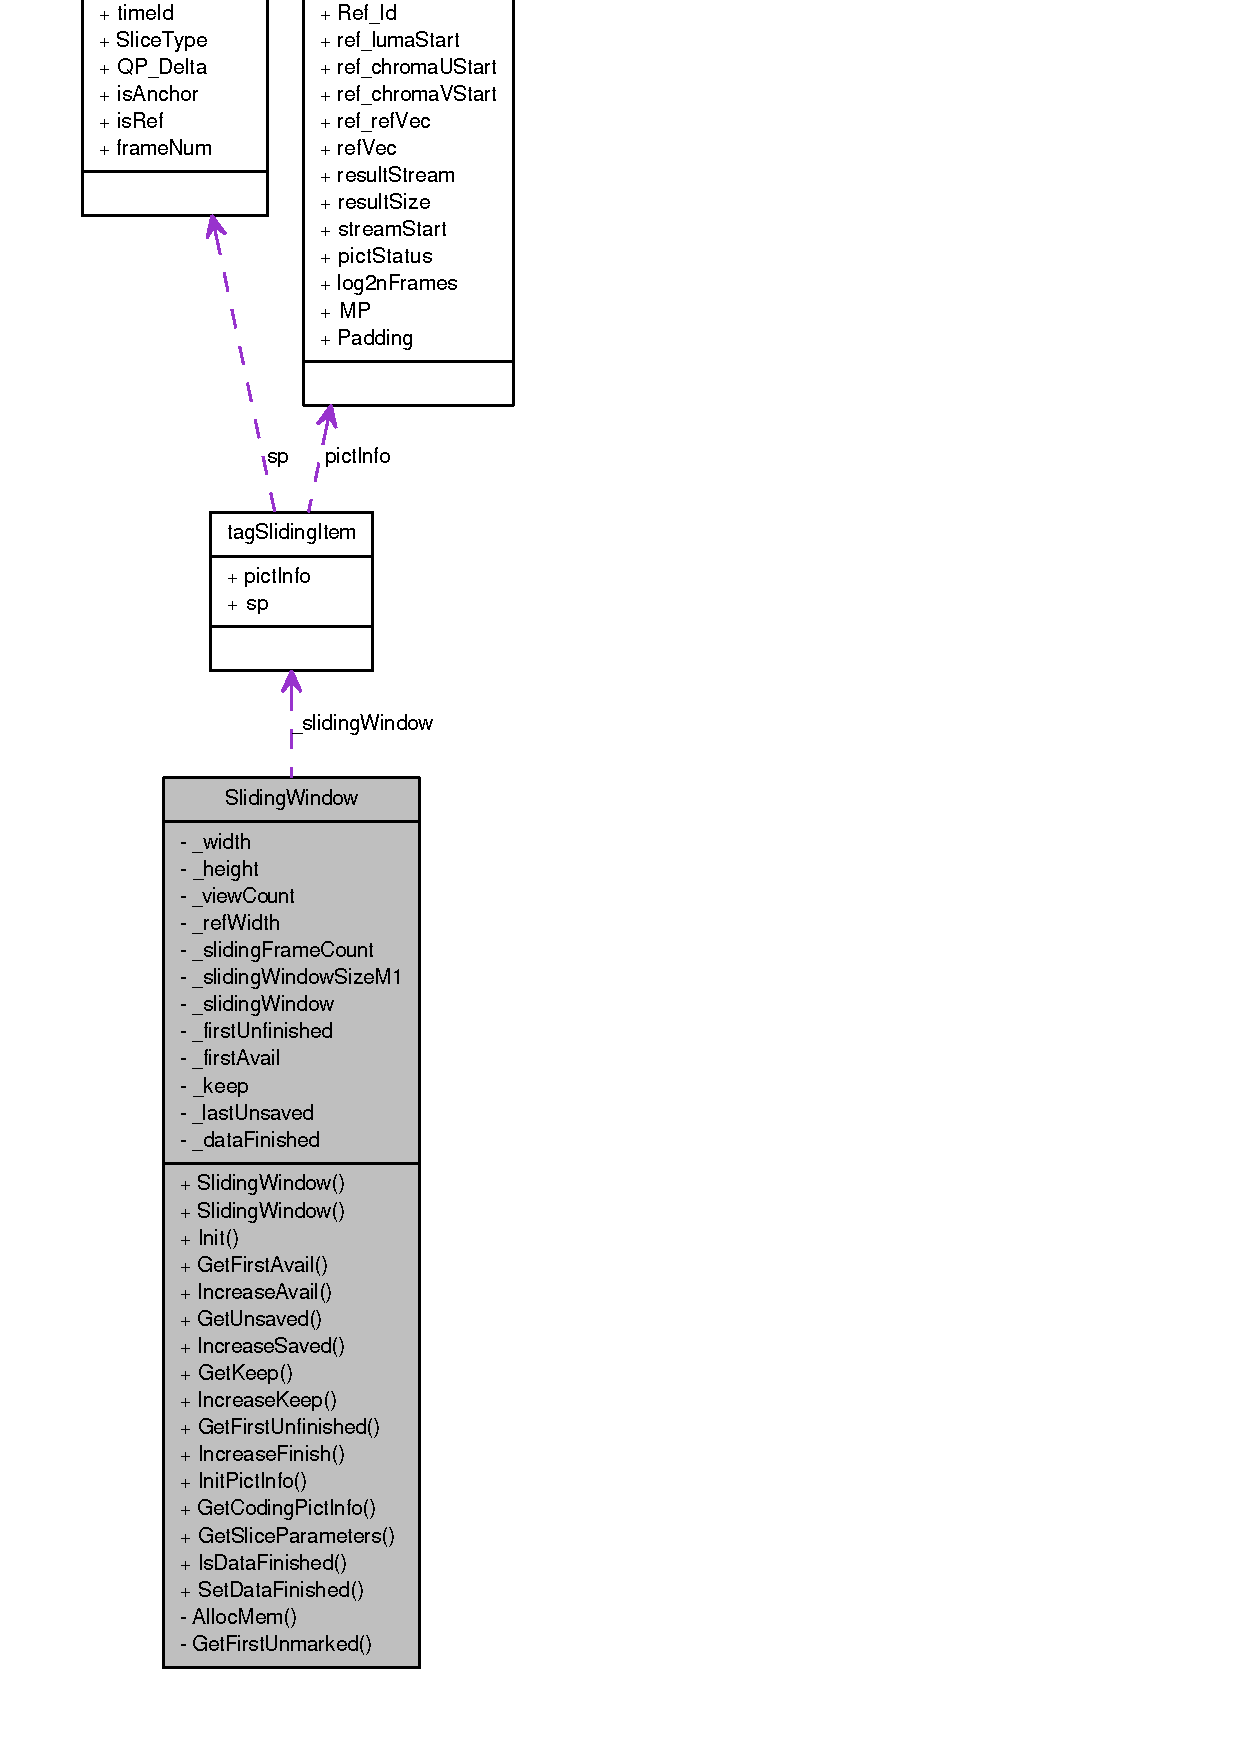
\includegraphics[height=400pt]{class_sliding_window__coll__graph}
\end{center}
\end{figure}
\subsection*{Public Member Functions}
\begin{DoxyCompactItemize}
\item 
\hyperlink{class_sliding_window_a5fde76017cc202055cf3ae3011258106}{SlidingWindow} ()
\item 
\hyperlink{class_sliding_window_aa833d1b81d72234b0e37364295820e96}{SlidingWindow} (int width, int height, int viewCount, int refWidth, int slidingFrameCount)
\item 
void \hyperlink{class_sliding_window_ac71c1ed41e1b33a1ef3623c881e6d9d7}{Init} (int width, int height, int viewCount, int refWidth, int slidingFrameCount)
\item 
int \hyperlink{class_sliding_window_a2128091c76b407cd0e244759ba5a2846}{GetFirstAvail} () const 
\item 
void \hyperlink{class_sliding_window_a7bce9e53d3618b89f47684ec1432848d}{IncreaseAvail} ()
\item 
int \hyperlink{class_sliding_window_a3df64e20282ce10a45c4c3f3011e536d}{GetUnsaved} ()
\item 
void \hyperlink{class_sliding_window_aea027ce6f77dcee09d1aafb31d5732c5}{IncreaseSaved} ()
\item 
int \hyperlink{class_sliding_window_a0aafbf41ff2b7bb6c32fb60075bfeb22}{GetKeep} ()
\item 
void \hyperlink{class_sliding_window_a9b7a7426f6a495da2770e0743d4c97d7}{IncreaseKeep} ()
\item 
int \hyperlink{class_sliding_window_a3be69abc76bff5b71ab96dadcced9f65}{GetFirstUnfinished} ()
\item 
void \hyperlink{class_sliding_window_a8f303bc211297021f20e09dced119207}{IncreaseFinish} ()
\item 
void \hyperlink{class_sliding_window_a012dbfd5902b37d5ce3d37a115d9a96e}{InitPictInfo} (int timeId, int viewId)
\item 
\hyperlink{struct_coding_pict_info}{CodingPictInfo} $\ast$ \hyperlink{class_sliding_window_ac50874323a2aaa4ef76fab47f80c9f92}{GetCodingPictInfo} (int timeId, int viewId)
\item 
\hyperlink{struct_slice_parameters}{SliceParameters} $\ast$ \hyperlink{class_sliding_window_a020d2c25f1bda31337f91bf9b1a809d1}{GetSliceParameters} (int timeId, int viewId)
\item 
bool \hyperlink{class_sliding_window_afd67521d283b68f9fbc769ee9c0ba4b4}{IsDataFinished} () const 
\item 
void \hyperlink{class_sliding_window_ac2fd5605777fc2f4fdff84282a8467f8}{SetDataFinished} ()
\end{DoxyCompactItemize}


\subsection{Constructor \& Destructor Documentation}
\hypertarget{class_sliding_window_a5fde76017cc202055cf3ae3011258106}{
\index{SlidingWindow@{SlidingWindow}!SlidingWindow@{SlidingWindow}}
\index{SlidingWindow@{SlidingWindow}!SlidingWindow@{SlidingWindow}}
\subsubsection[{SlidingWindow}]{\setlength{\rightskip}{0pt plus 5cm}SlidingWindow::SlidingWindow ()\hspace{0.3cm}{\ttfamily  \mbox{[}inline\mbox{]}}}}
\label{class_sliding_window_a5fde76017cc202055cf3ae3011258106}




\begin{footnotesize}\begin{alltt}
00081                 : \_slidingFrameCount(0), \_width(0), \_height(0), \_viewCount(0), \_r
      efWidth(0), \_dataFinished(\textcolor{keyword}{false})
00082         \{
00083                 \_firstUnfinished = 0;
00084                 \_firstAvail = 0;
00085                 \_keep = 0;
00086                 \_lastUnsaved = 0;
00087         \}
\end{alltt}\end{footnotesize}


\hypertarget{class_sliding_window_aa833d1b81d72234b0e37364295820e96}{
\index{SlidingWindow@{SlidingWindow}!SlidingWindow@{SlidingWindow}}
\index{SlidingWindow@{SlidingWindow}!SlidingWindow@{SlidingWindow}}
\subsubsection[{SlidingWindow}]{\setlength{\rightskip}{0pt plus 5cm}SlidingWindow::SlidingWindow (int {\em width}, \/  int {\em height}, \/  int {\em viewCount}, \/  int {\em refWidth}, \/  int {\em slidingFrameCount})\hspace{0.3cm}{\ttfamily  \mbox{[}inline\mbox{]}}}}
\label{class_sliding_window_aa833d1b81d72234b0e37364295820e96}




\begin{footnotesize}\begin{alltt}
00090                 : \_slidingFrameCount(0), \_width(0), \_height(0), \_viewCount(0), \_r
      efWidth(0), \_dataFinished(\textcolor{keyword}{false})
00091         \{
00092                 \hyperlink{class_sliding_window_ac71c1ed41e1b33a1ef3623c881e6d9d7}{Init}(width, height, viewCount, refWidth, slidingFrameCount);
00093                 \_firstUnfinished = 0;
00094                 \_firstAvail = 0;
00095                 \_keep = 0;
00096                 \_lastUnsaved = 0;
00097         \}
\end{alltt}\end{footnotesize}




Here is the call graph for this function:\nopagebreak
\begin{figure}[H]
\begin{center}
\leavevmode
\includegraphics[width=165pt]{class_sliding_window_aa833d1b81d72234b0e37364295820e96_cgraph}
\end{center}
\end{figure}




\subsection{Member Function Documentation}
\hypertarget{class_sliding_window_ac50874323a2aaa4ef76fab47f80c9f92}{
\index{SlidingWindow@{SlidingWindow}!GetCodingPictInfo@{GetCodingPictInfo}}
\index{GetCodingPictInfo@{GetCodingPictInfo}!SlidingWindow@{SlidingWindow}}
\subsubsection[{GetCodingPictInfo}]{\setlength{\rightskip}{0pt plus 5cm}{\bf CodingPictInfo}$\ast$ SlidingWindow::GetCodingPictInfo (int {\em timeId}, \/  int {\em viewId})\hspace{0.3cm}{\ttfamily  \mbox{[}inline\mbox{]}}}}
\label{class_sliding_window_ac50874323a2aaa4ef76fab47f80c9f92}




\begin{footnotesize}\begin{alltt}
00185         \{
00186                 \textcolor{keywordflow}{if} (timeId - \hyperlink{class_sliding_window_a3df64e20282ce10a45c4c3f3011e536d}{GetUnsaved}() >= \_slidingFrameCount)
00187                         \textcolor{keywordflow}{return} 0;
00188                 \textcolor{keywordtype}{int} offset = (timeId * \_viewCount + viewId) & \_slidingWindowSizeM
      1;
00189                 \textcolor{keywordflow}{return} &(\_slidingWindow[offset].\hyperlink{structtag_sliding_item_a3d1f87274664505c5fb9fe06d3cd16d3}{pictInfo});
00190         \}
\end{alltt}\end{footnotesize}




Here is the call graph for this function:\nopagebreak
\begin{figure}[H]
\begin{center}
\leavevmode
\includegraphics[width=366pt]{class_sliding_window_ac50874323a2aaa4ef76fab47f80c9f92_cgraph}
\end{center}
\end{figure}




Here is the caller graph for this function:\nopagebreak
\begin{figure}[H]
\begin{center}
\leavevmode
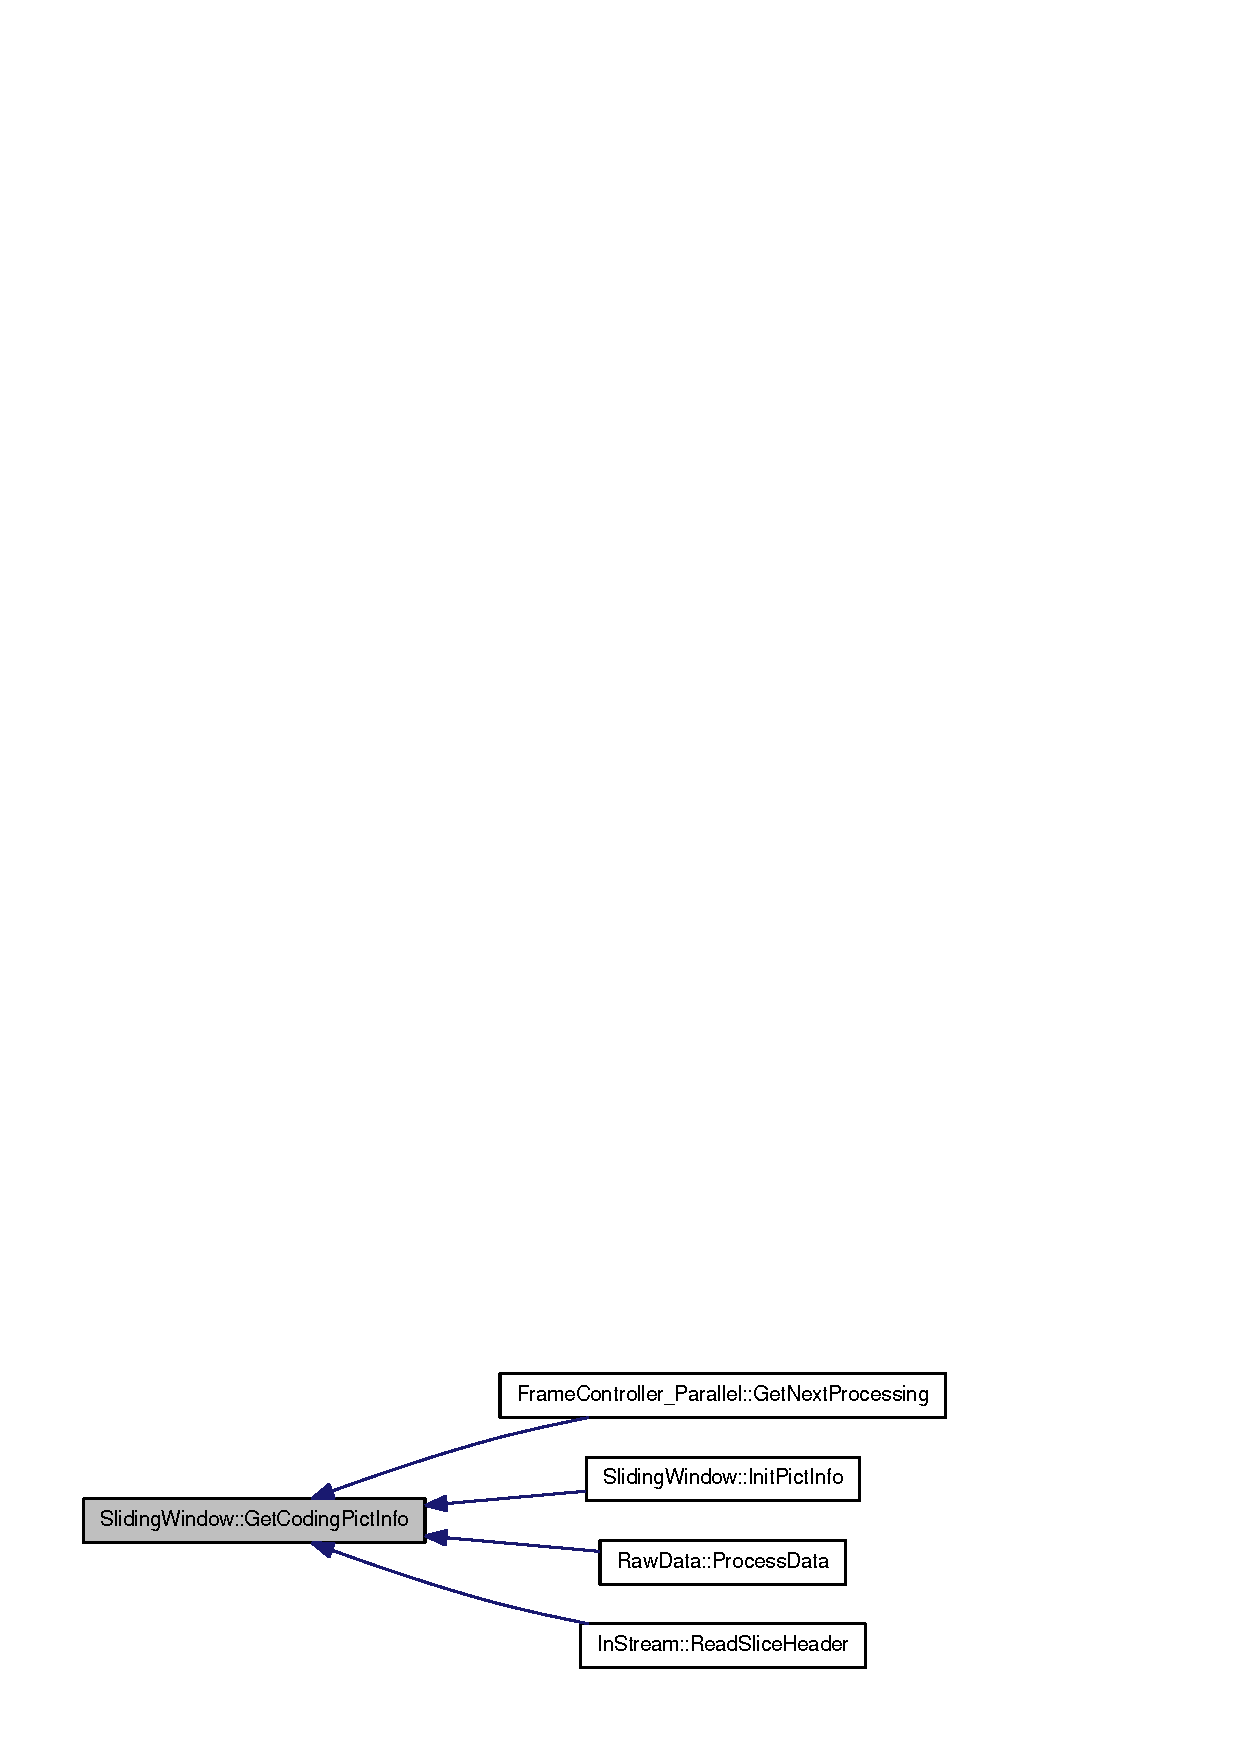
\includegraphics[width=229pt]{class_sliding_window_ac50874323a2aaa4ef76fab47f80c9f92_icgraph}
\end{center}
\end{figure}


\hypertarget{class_sliding_window_a2128091c76b407cd0e244759ba5a2846}{
\index{SlidingWindow@{SlidingWindow}!GetFirstAvail@{GetFirstAvail}}
\index{GetFirstAvail@{GetFirstAvail}!SlidingWindow@{SlidingWindow}}
\subsubsection[{GetFirstAvail}]{\setlength{\rightskip}{0pt plus 5cm}int SlidingWindow::GetFirstAvail () const\hspace{0.3cm}{\ttfamily  \mbox{[}inline\mbox{]}}}}
\label{class_sliding_window_a2128091c76b407cd0e244759ba5a2846}




\begin{footnotesize}\begin{alltt}
00120         \{
00121                 \textcolor{keywordflow}{return} \_firstAvail;
00122         \}
\end{alltt}\end{footnotesize}




Here is the caller graph for this function:\nopagebreak
\begin{figure}[H]
\begin{center}
\leavevmode
\includegraphics[width=218pt]{class_sliding_window_a2128091c76b407cd0e244759ba5a2846_icgraph}
\end{center}
\end{figure}


\hypertarget{class_sliding_window_a3be69abc76bff5b71ab96dadcced9f65}{
\index{SlidingWindow@{SlidingWindow}!GetFirstUnfinished@{GetFirstUnfinished}}
\index{GetFirstUnfinished@{GetFirstUnfinished}!SlidingWindow@{SlidingWindow}}
\subsubsection[{GetFirstUnfinished}]{\setlength{\rightskip}{0pt plus 5cm}int SlidingWindow::GetFirstUnfinished ()\hspace{0.3cm}{\ttfamily  \mbox{[}inline\mbox{]}}}}
\label{class_sliding_window_a3be69abc76bff5b71ab96dadcced9f65}




\begin{footnotesize}\begin{alltt}
00163         \{
00164                 \textcolor{keywordflow}{return} \_firstUnfinished;
00165         \}
\end{alltt}\end{footnotesize}




Here is the caller graph for this function:\nopagebreak
\begin{figure}[H]
\begin{center}
\leavevmode
\includegraphics[width=231pt]{class_sliding_window_a3be69abc76bff5b71ab96dadcced9f65_icgraph}
\end{center}
\end{figure}


\hypertarget{class_sliding_window_a0aafbf41ff2b7bb6c32fb60075bfeb22}{
\index{SlidingWindow@{SlidingWindow}!GetKeep@{GetKeep}}
\index{GetKeep@{GetKeep}!SlidingWindow@{SlidingWindow}}
\subsubsection[{GetKeep}]{\setlength{\rightskip}{0pt plus 5cm}int SlidingWindow::GetKeep ()\hspace{0.3cm}{\ttfamily  \mbox{[}inline\mbox{]}}}}
\label{class_sliding_window_a0aafbf41ff2b7bb6c32fb60075bfeb22}




\begin{footnotesize}\begin{alltt}
00151         \{
00152                 \textcolor{keywordflow}{if} (\_dataFinished && (\_firstUnfinished == \_firstAvail))
00153                         \_keep = \_firstUnfinished;
00154                 \textcolor{keywordflow}{return} \_keep;
00155         \}
\end{alltt}\end{footnotesize}




Here is the caller graph for this function:\nopagebreak
\begin{figure}[H]
\begin{center}
\leavevmode
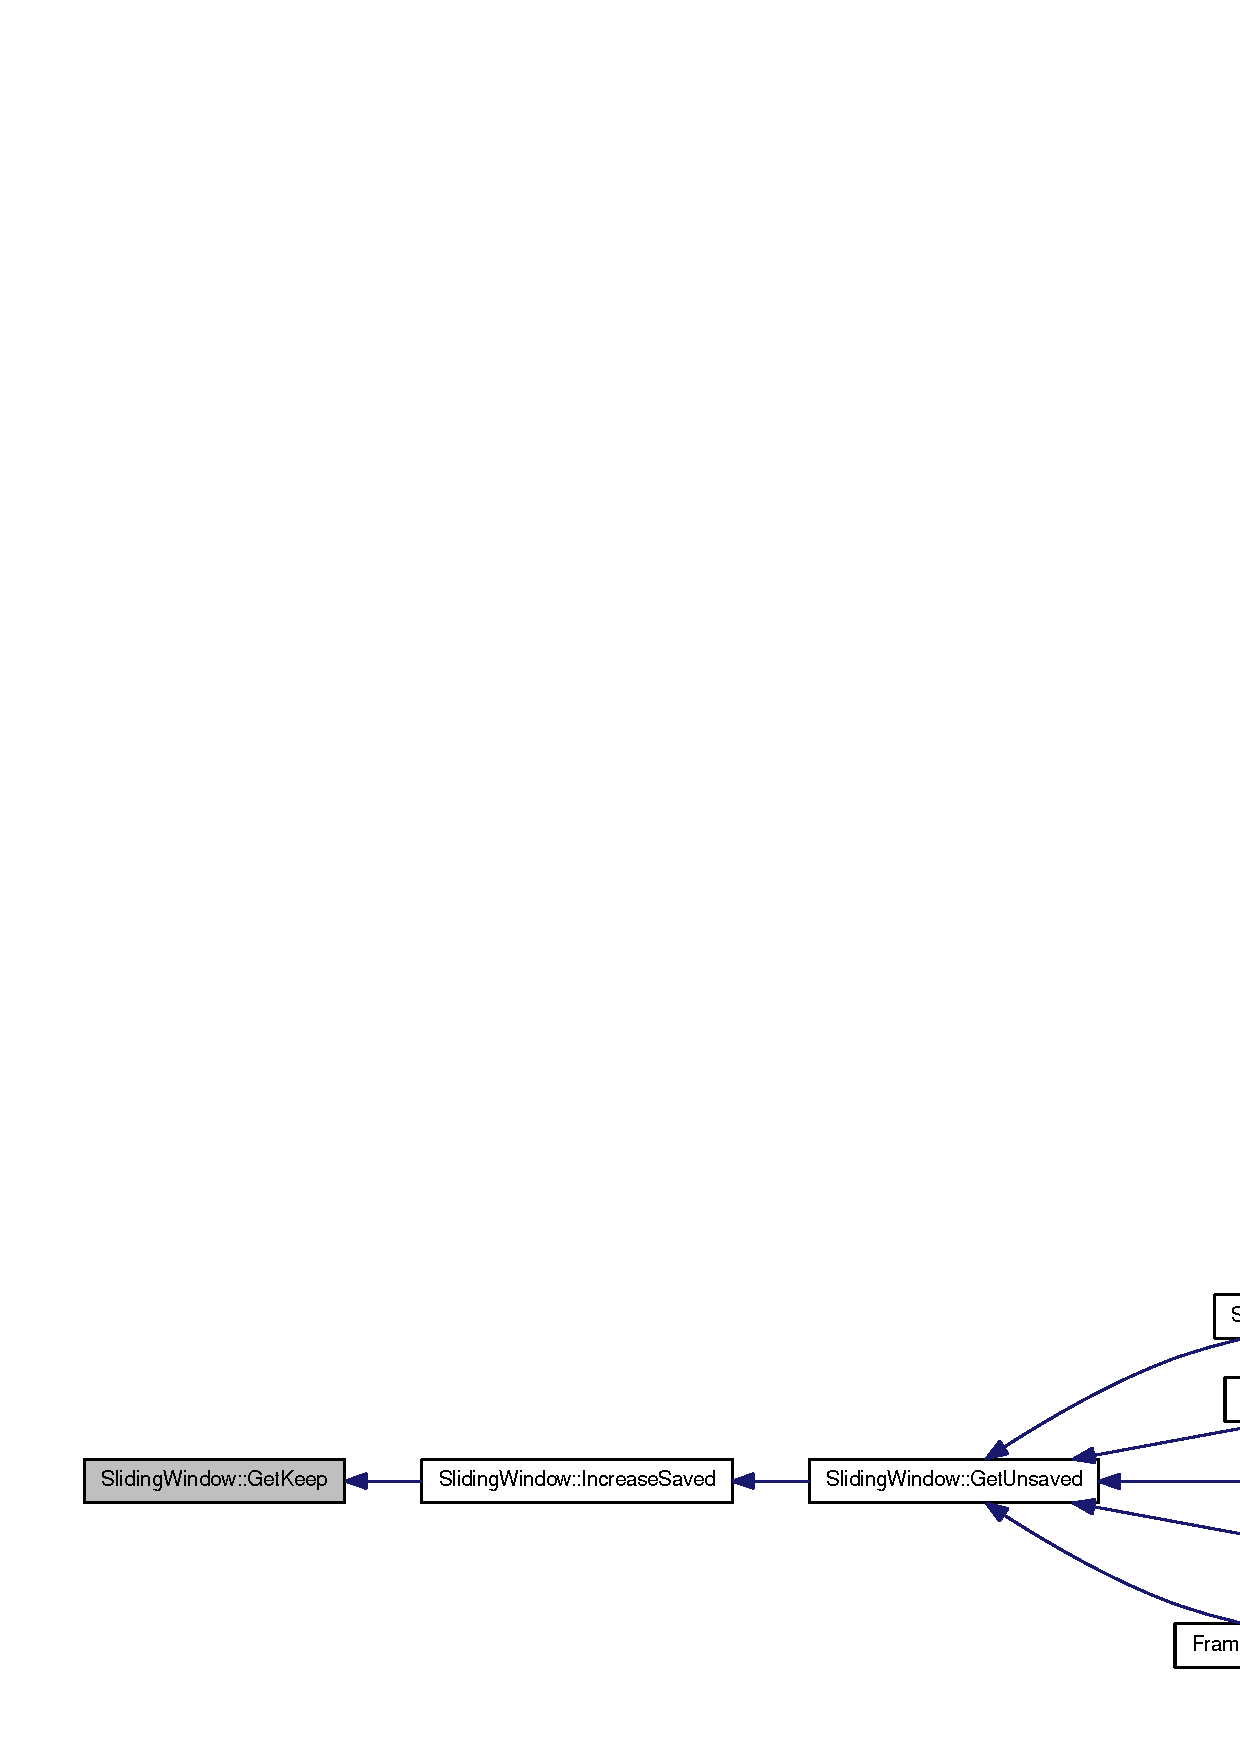
\includegraphics[width=420pt]{class_sliding_window_a0aafbf41ff2b7bb6c32fb60075bfeb22_icgraph}
\end{center}
\end{figure}


\hypertarget{class_sliding_window_a020d2c25f1bda31337f91bf9b1a809d1}{
\index{SlidingWindow@{SlidingWindow}!GetSliceParameters@{GetSliceParameters}}
\index{GetSliceParameters@{GetSliceParameters}!SlidingWindow@{SlidingWindow}}
\subsubsection[{GetSliceParameters}]{\setlength{\rightskip}{0pt plus 5cm}{\bf SliceParameters}$\ast$ SlidingWindow::GetSliceParameters (int {\em timeId}, \/  int {\em viewId})\hspace{0.3cm}{\ttfamily  \mbox{[}inline\mbox{]}}}}
\label{class_sliding_window_a020d2c25f1bda31337f91bf9b1a809d1}




\begin{footnotesize}\begin{alltt}
00193         \{
00194                 \textcolor{keywordflow}{if} (timeId - \hyperlink{class_sliding_window_a3df64e20282ce10a45c4c3f3011e536d}{GetUnsaved}() >= \_slidingFrameCount)
00195                         \textcolor{keywordflow}{return} 0;
00196                 \textcolor{keywordtype}{int} offset = (timeId * \_viewCount + viewId) & \_slidingWindowSizeM
      1;
00197                 \textcolor{keywordflow}{return} &(\_slidingWindow[offset].\hyperlink{structtag_sliding_item_a56c9f0817a904f6257d5de4e28c28724}{sp});
00198         \}
\end{alltt}\end{footnotesize}




Here is the call graph for this function:\nopagebreak
\begin{figure}[H]
\begin{center}
\leavevmode
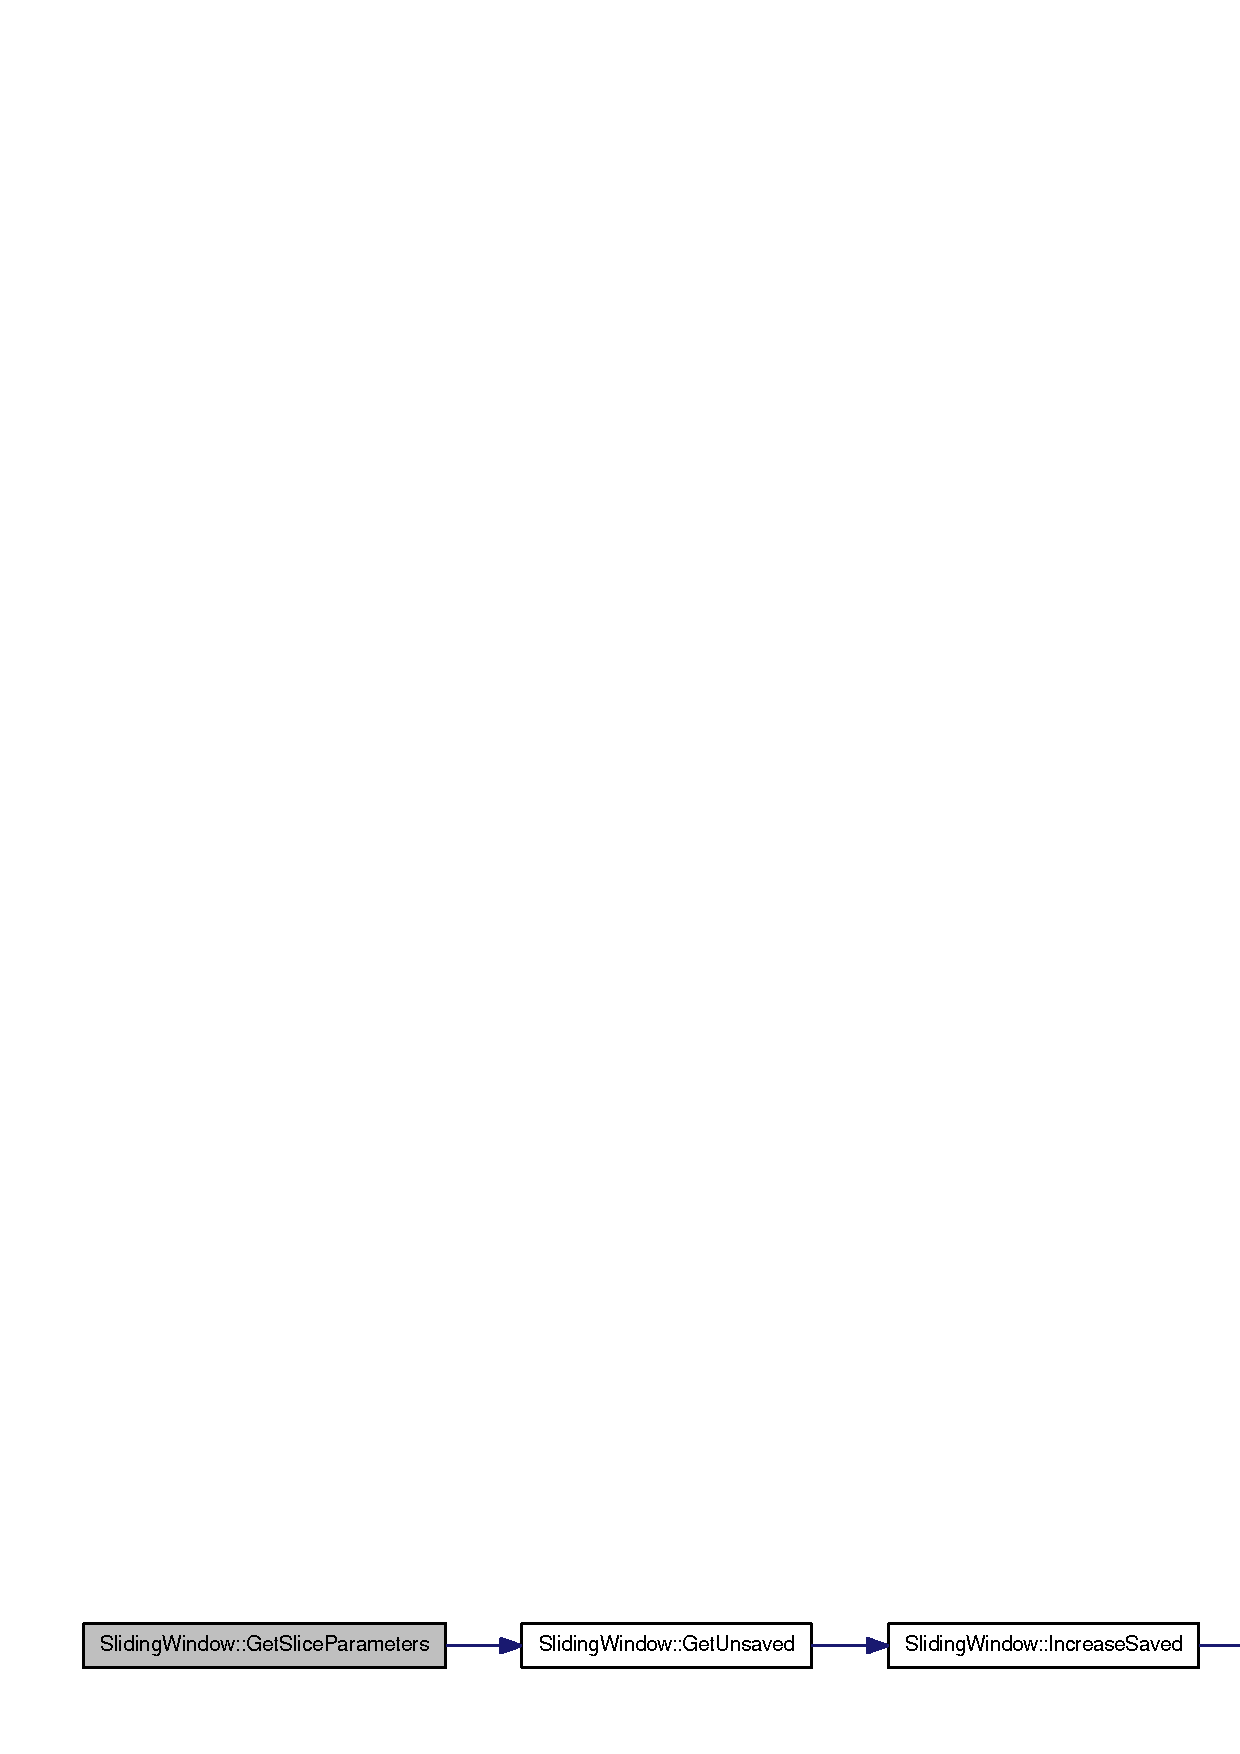
\includegraphics[width=371pt]{class_sliding_window_a020d2c25f1bda31337f91bf9b1a809d1_cgraph}
\end{center}
\end{figure}




Here is the caller graph for this function:\nopagebreak
\begin{figure}[H]
\begin{center}
\leavevmode
\includegraphics[width=234pt]{class_sliding_window_a020d2c25f1bda31337f91bf9b1a809d1_icgraph}
\end{center}
\end{figure}


\hypertarget{class_sliding_window_a3df64e20282ce10a45c4c3f3011e536d}{
\index{SlidingWindow@{SlidingWindow}!GetUnsaved@{GetUnsaved}}
\index{GetUnsaved@{GetUnsaved}!SlidingWindow@{SlidingWindow}}
\subsubsection[{GetUnsaved}]{\setlength{\rightskip}{0pt plus 5cm}int SlidingWindow::GetUnsaved ()\hspace{0.3cm}{\ttfamily  \mbox{[}inline\mbox{]}}}}
\label{class_sliding_window_a3df64e20282ce10a45c4c3f3011e536d}




\begin{footnotesize}\begin{alltt}
00130         \{
00131                 \hyperlink{class_sliding_window_aea027ce6f77dcee09d1aafb31d5732c5}{IncreaseSaved}();
00132                 \textcolor{keywordflow}{return} \_lastUnsaved;
00133         \}
\end{alltt}\end{footnotesize}




Here is the call graph for this function:\nopagebreak
\begin{figure}[H]
\begin{center}
\leavevmode
\includegraphics[width=266pt]{class_sliding_window_a3df64e20282ce10a45c4c3f3011e536d_cgraph}
\end{center}
\end{figure}




Here is the caller graph for this function:\nopagebreak
\begin{figure}[H]
\begin{center}
\leavevmode
\includegraphics[width=341pt]{class_sliding_window_a3df64e20282ce10a45c4c3f3011e536d_icgraph}
\end{center}
\end{figure}


\hypertarget{class_sliding_window_a7bce9e53d3618b89f47684ec1432848d}{
\index{SlidingWindow@{SlidingWindow}!IncreaseAvail@{IncreaseAvail}}
\index{IncreaseAvail@{IncreaseAvail}!SlidingWindow@{SlidingWindow}}
\subsubsection[{IncreaseAvail}]{\setlength{\rightskip}{0pt plus 5cm}void SlidingWindow::IncreaseAvail ()\hspace{0.3cm}{\ttfamily  \mbox{[}inline\mbox{]}}}}
\label{class_sliding_window_a7bce9e53d3618b89f47684ec1432848d}




\begin{footnotesize}\begin{alltt}
00125         \{
00126                 \_firstAvail = GetFirstUnmarked(\hyperlink{_picture_info_8h_aecbf7bf3158e75ca4906202b17b8f9ef}{PICT_STATUS_AVAIL}, \_firstAvail, 
      \hyperlink{class_sliding_window_a3df64e20282ce10a45c4c3f3011e536d}{GetUnsaved}() + \_slidingFrameCount);
00127         \}
\end{alltt}\end{footnotesize}




Here is the call graph for this function:\nopagebreak
\begin{figure}[H]
\begin{center}
\leavevmode
\includegraphics[width=356pt]{class_sliding_window_a7bce9e53d3618b89f47684ec1432848d_cgraph}
\end{center}
\end{figure}


\hypertarget{class_sliding_window_a8f303bc211297021f20e09dced119207}{
\index{SlidingWindow@{SlidingWindow}!IncreaseFinish@{IncreaseFinish}}
\index{IncreaseFinish@{IncreaseFinish}!SlidingWindow@{SlidingWindow}}
\subsubsection[{IncreaseFinish}]{\setlength{\rightskip}{0pt plus 5cm}void SlidingWindow::IncreaseFinish ()\hspace{0.3cm}{\ttfamily  \mbox{[}inline\mbox{]}}}}
\label{class_sliding_window_a8f303bc211297021f20e09dced119207}




\begin{footnotesize}\begin{alltt}
00168         \{
00169                 \_firstUnfinished = GetFirstUnmarked(\hyperlink{_picture_info_8h_a170d5962358e97425e08d5646653494b}{PICT_STATUS_FINISHED}, \_firstU
      nfinished, \_firstAvail);
00170                 \textcolor{keywordflow}{if} (\_dataFinished && (\_firstUnfinished == \_firstAvail))
00171                         \_keep = \_firstUnfinished;
00172                 \textcolor{keywordflow}{else} \textcolor{keywordflow}{if} (\_firstUnfinished - \_keep > \_refWidth)
00173                         \_keep = \_firstUnfinished - \_refWidth;
00174         \}
\end{alltt}\end{footnotesize}




Here is the caller graph for this function:\nopagebreak
\begin{figure}[H]
\begin{center}
\leavevmode
\includegraphics[width=221pt]{class_sliding_window_a8f303bc211297021f20e09dced119207_icgraph}
\end{center}
\end{figure}


\hypertarget{class_sliding_window_a9b7a7426f6a495da2770e0743d4c97d7}{
\index{SlidingWindow@{SlidingWindow}!IncreaseKeep@{IncreaseKeep}}
\index{IncreaseKeep@{IncreaseKeep}!SlidingWindow@{SlidingWindow}}
\subsubsection[{IncreaseKeep}]{\setlength{\rightskip}{0pt plus 5cm}void SlidingWindow::IncreaseKeep ()\hspace{0.3cm}{\ttfamily  \mbox{[}inline\mbox{]}}}}
\label{class_sliding_window_a9b7a7426f6a495da2770e0743d4c97d7}




\begin{footnotesize}\begin{alltt}
00158         \{
00159                 ++\_keep;
00160         \}
\end{alltt}\end{footnotesize}


\hypertarget{class_sliding_window_aea027ce6f77dcee09d1aafb31d5732c5}{
\index{SlidingWindow@{SlidingWindow}!IncreaseSaved@{IncreaseSaved}}
\index{IncreaseSaved@{IncreaseSaved}!SlidingWindow@{SlidingWindow}}
\subsubsection[{IncreaseSaved}]{\setlength{\rightskip}{0pt plus 5cm}void SlidingWindow::IncreaseSaved ()\hspace{0.3cm}{\ttfamily  \mbox{[}inline\mbox{]}}}}
\label{class_sliding_window_aea027ce6f77dcee09d1aafb31d5732c5}




\begin{footnotesize}\begin{alltt}
00136         \{
00137                 \textcolor{keywordtype}{int} lastUnsaved = GetFirstUnmarked(\hyperlink{_picture_info_8h_a81f2be9d3984eb16fa6f3b7daf46466f}{PICT_STATUS_SAVED}, \_lastUnsave
      d, \hyperlink{class_sliding_window_a0aafbf41ff2b7bb6c32fb60075bfeb22}{GetKeep}());
00138                 \textcolor{keywordtype}{int} offset = (\_lastUnsaved * \_viewCount) & \_slidingWindowSizeM1;
00139                 \textcolor{keywordflow}{for} (\textcolor{keywordtype}{int} i = \_lastUnsaved; i < lastUnsaved; ++i)
00140                 \{
00141                         \textcolor{keywordflow}{for} (\textcolor{keywordtype}{int} j = 0; j < \_viewCount; ++j)
00142                         \{
00143                                 \_slidingWindow[offset].\hyperlink{structtag_sliding_item_a3d1f87274664505c5fb9fe06d3cd16d3}{pictInfo}.\hyperlink{struct_coding_pict_info_a41498e5ba764405481005e6569d7f728}{pictStatus} = 
      \hyperlink{_picture_info_8h_ac2f16d038f94c6c57ed8648c6cfe3bb7}{PICT_STATUS_WAIT};
00144                                 offset = (offset + 1) & \_slidingWindowSizeM1;
00145                         \}
00146                 \}
00147                 \_lastUnsaved = lastUnsaved;
00148         \}
\end{alltt}\end{footnotesize}




Here is the call graph for this function:\nopagebreak
\begin{figure}[H]
\begin{center}
\leavevmode
\includegraphics[width=178pt]{class_sliding_window_aea027ce6f77dcee09d1aafb31d5732c5_cgraph}
\end{center}
\end{figure}




Here is the caller graph for this function:\nopagebreak
\begin{figure}[H]
\begin{center}
\leavevmode
\includegraphics[width=420pt]{class_sliding_window_aea027ce6f77dcee09d1aafb31d5732c5_icgraph}
\end{center}
\end{figure}


\hypertarget{class_sliding_window_ac71c1ed41e1b33a1ef3623c881e6d9d7}{
\index{SlidingWindow@{SlidingWindow}!Init@{Init}}
\index{Init@{Init}!SlidingWindow@{SlidingWindow}}
\subsubsection[{Init}]{\setlength{\rightskip}{0pt plus 5cm}void SlidingWindow::Init (int {\em width}, \/  int {\em height}, \/  int {\em viewCount}, \/  int {\em refWidth}, \/  int {\em slidingFrameCount})\hspace{0.3cm}{\ttfamily  \mbox{[}inline\mbox{]}}}}
\label{class_sliding_window_ac71c1ed41e1b33a1ef3623c881e6d9d7}




\begin{footnotesize}\begin{alltt}
00100         \{
00101                 refWidth = refWidth * 2;
00102                 slidingFrameCount = refWidth * 2;
00103                 \_slidingFrameCount = slidingFrameCount;
00104                 \_width = width;
00105                 \_height = height;
00106                 \_viewCount = viewCount;
00107                 \_refWidth = refWidth;
00108                 \textcolor{keywordtype}{int} slidingWindowSize = \_viewCount * slidingFrameCount;
00109                 ++slidingWindowSize;
00110                 \textcolor{keywordflow}{while} (slidingWindowSize & (slidingWindowSize - 1))
00111                         slidingWindowSize = (slidingWindowSize | (slidingWindowSi
      ze - 1)) + 1;
00112                 printf(\textcolor{stringliteral}{"slidingWindowSize = %d\(\backslash\)n"}, slidingWindowSize);
00113                 \_slidingWindow = \textcolor{keyword}{new} \hyperlink{structtag_sliding_item}{SlidingItem}[slidingWindowSize];
00114                 \textcolor{keywordflow}{for} (\textcolor{keywordtype}{int} i = 0; i < slidingWindowSize; ++i)
00115                         AllocMem(\_slidingWindow[i].pictInfo);
00116                 \_slidingWindowSizeM1 = slidingWindowSize - 1;
00117         \}
\end{alltt}\end{footnotesize}




Here is the caller graph for this function:\nopagebreak
\begin{figure}[H]
\begin{center}
\leavevmode
\includegraphics[width=165pt]{class_sliding_window_ac71c1ed41e1b33a1ef3623c881e6d9d7_icgraph}
\end{center}
\end{figure}


\hypertarget{class_sliding_window_a012dbfd5902b37d5ce3d37a115d9a96e}{
\index{SlidingWindow@{SlidingWindow}!InitPictInfo@{InitPictInfo}}
\index{InitPictInfo@{InitPictInfo}!SlidingWindow@{SlidingWindow}}
\subsubsection[{InitPictInfo}]{\setlength{\rightskip}{0pt plus 5cm}void SlidingWindow::InitPictInfo (int {\em timeId}, \/  int {\em viewId})\hspace{0.3cm}{\ttfamily  \mbox{[}inline\mbox{]}}}}
\label{class_sliding_window_a012dbfd5902b37d5ce3d37a115d9a96e}




\begin{footnotesize}\begin{alltt}
00177         \{
00178                 \hyperlink{struct_coding_pict_info}{CodingPictInfo} &info = *\hyperlink{class_sliding_window_ac50874323a2aaa4ef76fab47f80c9f92}{GetCodingPictInfo}(timeId, viewId);
00179                 info.\hyperlink{struct_coding_pict_info_ad85dae4751165ea3cbb8f7b8c6e61dc3}{timeId} = timeId;
00180                 info.\hyperlink{struct_coding_pict_info_a987595091bfba91b3166b04bca988697}{viewId} = viewId;
00181                 info.\hyperlink{struct_coding_pict_info_a41498e5ba764405481005e6569d7f728}{pictStatus} = \hyperlink{_picture_info_8h_ac2f16d038f94c6c57ed8648c6cfe3bb7}{PICT_STATUS_WAIT};
00182         \}
\end{alltt}\end{footnotesize}




Here is the call graph for this function:\nopagebreak
\begin{figure}[H]
\begin{center}
\leavevmode
\includegraphics[width=420pt]{class_sliding_window_a012dbfd5902b37d5ce3d37a115d9a96e_cgraph}
\end{center}
\end{figure}


\hypertarget{class_sliding_window_afd67521d283b68f9fbc769ee9c0ba4b4}{
\index{SlidingWindow@{SlidingWindow}!IsDataFinished@{IsDataFinished}}
\index{IsDataFinished@{IsDataFinished}!SlidingWindow@{SlidingWindow}}
\subsubsection[{IsDataFinished}]{\setlength{\rightskip}{0pt plus 5cm}bool SlidingWindow::IsDataFinished () const\hspace{0.3cm}{\ttfamily  \mbox{[}inline\mbox{]}}}}
\label{class_sliding_window_afd67521d283b68f9fbc769ee9c0ba4b4}




\begin{footnotesize}\begin{alltt}
00201         \{
00202                 \textcolor{keywordflow}{return} \_dataFinished;
00203         \}
\end{alltt}\end{footnotesize}




Here is the caller graph for this function:\nopagebreak
\begin{figure}[H]
\begin{center}
\leavevmode
\includegraphics[width=222pt]{class_sliding_window_afd67521d283b68f9fbc769ee9c0ba4b4_icgraph}
\end{center}
\end{figure}


\hypertarget{class_sliding_window_ac2fd5605777fc2f4fdff84282a8467f8}{
\index{SlidingWindow@{SlidingWindow}!SetDataFinished@{SetDataFinished}}
\index{SetDataFinished@{SetDataFinished}!SlidingWindow@{SlidingWindow}}
\subsubsection[{SetDataFinished}]{\setlength{\rightskip}{0pt plus 5cm}void SlidingWindow::SetDataFinished ()\hspace{0.3cm}{\ttfamily  \mbox{[}inline\mbox{]}}}}
\label{class_sliding_window_ac2fd5605777fc2f4fdff84282a8467f8}




\begin{footnotesize}\begin{alltt}
00206         \{
00207                 \_dataFinished = \textcolor{keyword}{true};
00208         \}
\end{alltt}\end{footnotesize}




The documentation for this class was generated from the following file:\begin{DoxyCompactItemize}
\item 
MVCCommonLib/\hyperlink{_sliding_window_8h}{SlidingWindow.h}\end{DoxyCompactItemize}

\hypertarget{structtag__cavlc__ref}{
\section{tag\_\-cavlc\_\-ref Struct Reference}
\label{structtag__cavlc__ref}\index{tag\_\-cavlc\_\-ref@{tag\_\-cavlc\_\-ref}}
}


{\ttfamily \#include $<$vlcPred.h$>$}

\subsection*{Public Attributes}
\begin{DoxyCompactItemize}
\item 
int \hyperlink{structtag__cavlc__ref_a071bb830fe08f1df5618d391ed428221}{refid} \mbox{[}2\mbox{]}
\item 
int \hyperlink{structtag__cavlc__ref_a890a9186d3db3787c7a451e51f4fc0bf}{mv\_\-x} \mbox{[}2\mbox{]}
\item 
int \hyperlink{structtag__cavlc__ref_abae0c90668fedb380b2cc0773cfa351d}{mv\_\-y} \mbox{[}2\mbox{]}
\item 
int \hyperlink{structtag__cavlc__ref_a4fc396cd8d03fbd50466ff12a4785529}{coeff}
\item 
int \hyperlink{structtag__cavlc__ref_a38397a4aa7f4f450d2bed25146783b22}{coeffC}
\item 
int \hyperlink{structtag__cavlc__ref_a76c8b0c75a3a13a59196c89cf919766f}{imode}
\end{DoxyCompactItemize}


\subsection{Member Data Documentation}
\hypertarget{structtag__cavlc__ref_a4fc396cd8d03fbd50466ff12a4785529}{
\index{tag\_\-cavlc\_\-ref@{tag\_\-cavlc\_\-ref}!coeff@{coeff}}
\index{coeff@{coeff}!tag_cavlc_ref@{tag\_\-cavlc\_\-ref}}
\subsubsection[{coeff}]{\setlength{\rightskip}{0pt plus 5cm}int {\bf tag\_\-cavlc\_\-ref::coeff}}}
\label{structtag__cavlc__ref_a4fc396cd8d03fbd50466ff12a4785529}
\hypertarget{structtag__cavlc__ref_a38397a4aa7f4f450d2bed25146783b22}{
\index{tag\_\-cavlc\_\-ref@{tag\_\-cavlc\_\-ref}!coeffC@{coeffC}}
\index{coeffC@{coeffC}!tag_cavlc_ref@{tag\_\-cavlc\_\-ref}}
\subsubsection[{coeffC}]{\setlength{\rightskip}{0pt plus 5cm}int {\bf tag\_\-cavlc\_\-ref::coeffC}}}
\label{structtag__cavlc__ref_a38397a4aa7f4f450d2bed25146783b22}
\hypertarget{structtag__cavlc__ref_a76c8b0c75a3a13a59196c89cf919766f}{
\index{tag\_\-cavlc\_\-ref@{tag\_\-cavlc\_\-ref}!imode@{imode}}
\index{imode@{imode}!tag_cavlc_ref@{tag\_\-cavlc\_\-ref}}
\subsubsection[{imode}]{\setlength{\rightskip}{0pt plus 5cm}int {\bf tag\_\-cavlc\_\-ref::imode}}}
\label{structtag__cavlc__ref_a76c8b0c75a3a13a59196c89cf919766f}
\hypertarget{structtag__cavlc__ref_a890a9186d3db3787c7a451e51f4fc0bf}{
\index{tag\_\-cavlc\_\-ref@{tag\_\-cavlc\_\-ref}!mv\_\-x@{mv\_\-x}}
\index{mv\_\-x@{mv\_\-x}!tag_cavlc_ref@{tag\_\-cavlc\_\-ref}}
\subsubsection[{mv\_\-x}]{\setlength{\rightskip}{0pt plus 5cm}int {\bf tag\_\-cavlc\_\-ref::mv\_\-x}\mbox{[}2\mbox{]}}}
\label{structtag__cavlc__ref_a890a9186d3db3787c7a451e51f4fc0bf}
\hypertarget{structtag__cavlc__ref_abae0c90668fedb380b2cc0773cfa351d}{
\index{tag\_\-cavlc\_\-ref@{tag\_\-cavlc\_\-ref}!mv\_\-y@{mv\_\-y}}
\index{mv\_\-y@{mv\_\-y}!tag_cavlc_ref@{tag\_\-cavlc\_\-ref}}
\subsubsection[{mv\_\-y}]{\setlength{\rightskip}{0pt plus 5cm}int {\bf tag\_\-cavlc\_\-ref::mv\_\-y}\mbox{[}2\mbox{]}}}
\label{structtag__cavlc__ref_abae0c90668fedb380b2cc0773cfa351d}
\hypertarget{structtag__cavlc__ref_a071bb830fe08f1df5618d391ed428221}{
\index{tag\_\-cavlc\_\-ref@{tag\_\-cavlc\_\-ref}!refid@{refid}}
\index{refid@{refid}!tag_cavlc_ref@{tag\_\-cavlc\_\-ref}}
\subsubsection[{refid}]{\setlength{\rightskip}{0pt plus 5cm}int {\bf tag\_\-cavlc\_\-ref::refid}\mbox{[}2\mbox{]}}}
\label{structtag__cavlc__ref_a071bb830fe08f1df5618d391ed428221}


The documentation for this struct was generated from the following file:\begin{DoxyCompactItemize}
\item 
MVCCommonLib/Codec/\hyperlink{vlc_pred_8h}{vlcPred.h}\end{DoxyCompactItemize}

\hypertarget{structtag__cavlc__ref__list}{
\section{tag\_\-cavlc\_\-ref\_\-list Struct Reference}
\label{structtag__cavlc__ref__list}\index{tag\_\-cavlc\_\-ref\_\-list@{tag\_\-cavlc\_\-ref\_\-list}}
}


{\ttfamily \#include $<$vlcPred.h$>$}



Collaboration diagram for tag\_\-cavlc\_\-ref\_\-list:\nopagebreak
\begin{figure}[H]
\begin{center}
\leavevmode
\includegraphics[width=134pt]{structtag__cavlc__ref__list__coll__graph}
\end{center}
\end{figure}
\subsection*{Public Attributes}
\begin{DoxyCompactItemize}
\item 
\hyperlink{structtag__cavlc__ref}{cavlc\_\-ref} $\ast$ \hyperlink{structtag__cavlc__ref__list_a854c970004394513901757cc3dcb65e5}{left}
\item 
\hyperlink{structtag__cavlc__ref}{cavlc\_\-ref} $\ast$ \hyperlink{structtag__cavlc__ref__list_af93b34de26224281e33b951333a665c7}{top}
\item 
\hyperlink{structtag__cavlc__ref}{cavlc\_\-ref} \hyperlink{structtag__cavlc__ref__list_ac71d66d925cb5fbc0c15812f70aa2e78}{topleft}
\item 
\hyperlink{structtag__cavlc__ref}{cavlc\_\-ref} \hyperlink{structtag__cavlc__ref__list_ae9fad3ab9c8086e7dd826492ee027b7d}{lefts} \mbox{[}4\mbox{]}
\item 
\hyperlink{structtag__cavlc__ref}{cavlc\_\-ref} \hyperlink{structtag__cavlc__ref__list_ab4d9282dda63bfa7f48cff76db26de04}{tops} \mbox{[}5\mbox{]}
\end{DoxyCompactItemize}


\subsection{Member Data Documentation}
\hypertarget{structtag__cavlc__ref__list_a854c970004394513901757cc3dcb65e5}{
\index{tag\_\-cavlc\_\-ref\_\-list@{tag\_\-cavlc\_\-ref\_\-list}!left@{left}}
\index{left@{left}!tag_cavlc_ref_list@{tag\_\-cavlc\_\-ref\_\-list}}
\subsubsection[{left}]{\setlength{\rightskip}{0pt plus 5cm}{\bf cavlc\_\-ref}$\ast$ {\bf tag\_\-cavlc\_\-ref\_\-list::left}}}
\label{structtag__cavlc__ref__list_a854c970004394513901757cc3dcb65e5}
\hypertarget{structtag__cavlc__ref__list_ae9fad3ab9c8086e7dd826492ee027b7d}{
\index{tag\_\-cavlc\_\-ref\_\-list@{tag\_\-cavlc\_\-ref\_\-list}!lefts@{lefts}}
\index{lefts@{lefts}!tag_cavlc_ref_list@{tag\_\-cavlc\_\-ref\_\-list}}
\subsubsection[{lefts}]{\setlength{\rightskip}{0pt plus 5cm}{\bf cavlc\_\-ref} {\bf tag\_\-cavlc\_\-ref\_\-list::lefts}\mbox{[}4\mbox{]}}}
\label{structtag__cavlc__ref__list_ae9fad3ab9c8086e7dd826492ee027b7d}
\hypertarget{structtag__cavlc__ref__list_af93b34de26224281e33b951333a665c7}{
\index{tag\_\-cavlc\_\-ref\_\-list@{tag\_\-cavlc\_\-ref\_\-list}!top@{top}}
\index{top@{top}!tag_cavlc_ref_list@{tag\_\-cavlc\_\-ref\_\-list}}
\subsubsection[{top}]{\setlength{\rightskip}{0pt plus 5cm}{\bf cavlc\_\-ref}$\ast$ {\bf tag\_\-cavlc\_\-ref\_\-list::top}}}
\label{structtag__cavlc__ref__list_af93b34de26224281e33b951333a665c7}
\hypertarget{structtag__cavlc__ref__list_ac71d66d925cb5fbc0c15812f70aa2e78}{
\index{tag\_\-cavlc\_\-ref\_\-list@{tag\_\-cavlc\_\-ref\_\-list}!topleft@{topleft}}
\index{topleft@{topleft}!tag_cavlc_ref_list@{tag\_\-cavlc\_\-ref\_\-list}}
\subsubsection[{topleft}]{\setlength{\rightskip}{0pt plus 5cm}{\bf cavlc\_\-ref} {\bf tag\_\-cavlc\_\-ref\_\-list::topleft}}}
\label{structtag__cavlc__ref__list_ac71d66d925cb5fbc0c15812f70aa2e78}
\hypertarget{structtag__cavlc__ref__list_ab4d9282dda63bfa7f48cff76db26de04}{
\index{tag\_\-cavlc\_\-ref\_\-list@{tag\_\-cavlc\_\-ref\_\-list}!tops@{tops}}
\index{tops@{tops}!tag_cavlc_ref_list@{tag\_\-cavlc\_\-ref\_\-list}}
\subsubsection[{tops}]{\setlength{\rightskip}{0pt plus 5cm}{\bf cavlc\_\-ref} {\bf tag\_\-cavlc\_\-ref\_\-list::tops}\mbox{[}5\mbox{]}}}
\label{structtag__cavlc__ref__list_ab4d9282dda63bfa7f48cff76db26de04}


The documentation for this struct was generated from the following file:\begin{DoxyCompactItemize}
\item 
MVCCommonLib/Codec/\hyperlink{vlc_pred_8h}{vlcPred.h}\end{DoxyCompactItemize}

\hypertarget{structtag__macroblock__info}{
\section{tag\_\-macroblock\_\-info Struct Reference}
\label{structtag__macroblock__info}\index{tag\_\-macroblock\_\-info@{tag\_\-macroblock\_\-info}}
}


Collaboration diagram for tag\_\-macroblock\_\-info:\nopagebreak
\begin{figure}[H]
\begin{center}
\leavevmode
\includegraphics[height=400pt]{structtag__macroblock__info__coll__graph}
\end{center}
\end{figure}
\subsection*{Public Attributes}
\begin{DoxyCompactItemize}
\item 
\hyperlink{struct_coding_pict_info}{CodingPictInfo} $\ast$ \hyperlink{structtag__macroblock__info_ae7a0c6b68c7cbc0ffb1a82799eb386ef}{cpi}
\item 
\hyperlink{structmacroblock_info}{macroblockInfo} $\ast$ \hyperlink{structtag__macroblock__info_a150f68ca8a911ab2443199821f7b97e5}{mblist}
\item 
int \hyperlink{structtag__macroblock__info_a0431b0abc33b349505f0b83fd1537473}{row}
\item 
int \hyperlink{structtag__macroblock__info_affbe6dcc30999a24be78a7deb7a0e78b}{allow}
\item 
struct \hyperlink{structtag__macroblock__info}{tag\_\-macroblock\_\-info} $\ast$ \hyperlink{structtag__macroblock__info_ae6d03b766139a5abf281211e48c8d49b}{next}
\end{DoxyCompactItemize}


\subsection{Member Data Documentation}
\hypertarget{structtag__macroblock__info_affbe6dcc30999a24be78a7deb7a0e78b}{
\index{tag\_\-macroblock\_\-info@{tag\_\-macroblock\_\-info}!allow@{allow}}
\index{allow@{allow}!tag_macroblock_info@{tag\_\-macroblock\_\-info}}
\subsubsection[{allow}]{\setlength{\rightskip}{0pt plus 5cm}int {\bf tag\_\-macroblock\_\-info::allow}}}
\label{structtag__macroblock__info_affbe6dcc30999a24be78a7deb7a0e78b}
\hypertarget{structtag__macroblock__info_ae7a0c6b68c7cbc0ffb1a82799eb386ef}{
\index{tag\_\-macroblock\_\-info@{tag\_\-macroblock\_\-info}!cpi@{cpi}}
\index{cpi@{cpi}!tag_macroblock_info@{tag\_\-macroblock\_\-info}}
\subsubsection[{cpi}]{\setlength{\rightskip}{0pt plus 5cm}{\bf CodingPictInfo} $\ast$ {\bf tag\_\-macroblock\_\-info::cpi}}}
\label{structtag__macroblock__info_ae7a0c6b68c7cbc0ffb1a82799eb386ef}
\hypertarget{structtag__macroblock__info_a150f68ca8a911ab2443199821f7b97e5}{
\index{tag\_\-macroblock\_\-info@{tag\_\-macroblock\_\-info}!mblist@{mblist}}
\index{mblist@{mblist}!tag_macroblock_info@{tag\_\-macroblock\_\-info}}
\subsubsection[{mblist}]{\setlength{\rightskip}{0pt plus 5cm}{\bf macroblockInfo} $\ast$ {\bf tag\_\-macroblock\_\-info::mblist}}}
\label{structtag__macroblock__info_a150f68ca8a911ab2443199821f7b97e5}
\hypertarget{structtag__macroblock__info_ae6d03b766139a5abf281211e48c8d49b}{
\index{tag\_\-macroblock\_\-info@{tag\_\-macroblock\_\-info}!next@{next}}
\index{next@{next}!tag_macroblock_info@{tag\_\-macroblock\_\-info}}
\subsubsection[{next}]{\setlength{\rightskip}{0pt plus 5cm}struct {\bf tag\_\-macroblock\_\-info} $\ast$ {\bf tag\_\-macroblock\_\-info::next}}}
\label{structtag__macroblock__info_ae6d03b766139a5abf281211e48c8d49b}
\hypertarget{structtag__macroblock__info_a0431b0abc33b349505f0b83fd1537473}{
\index{tag\_\-macroblock\_\-info@{tag\_\-macroblock\_\-info}!row@{row}}
\index{row@{row}!tag_macroblock_info@{tag\_\-macroblock\_\-info}}
\subsubsection[{row}]{\setlength{\rightskip}{0pt plus 5cm}int {\bf tag\_\-macroblock\_\-info::row}}}
\label{structtag__macroblock__info_a0431b0abc33b349505f0b83fd1537473}


The documentation for this struct was generated from the following files:\begin{DoxyCompactItemize}
\item 
MVCDecoder/Codec/IFrame/\hyperlink{_i_slice_8cpp}{ISlice.cpp}\item 
MVCDecoder/Codec/PBFrame/\hyperlink{_p_slice_8cpp}{PSlice.cpp}\end{DoxyCompactItemize}

\hypertarget{structtag_sliding_item}{
\section{tagSlidingItem Struct Reference}
\label{structtag_sliding_item}\index{tagSlidingItem@{tagSlidingItem}}
}


{\ttfamily \#include $<$SlidingWindow.h$>$}



Collaboration diagram for tagSlidingItem:\nopagebreak
\begin{figure}[H]
\begin{center}
\leavevmode
\includegraphics[height=400pt]{structtag_sliding_item__coll__graph}
\end{center}
\end{figure}
\subsection*{Public Attributes}
\begin{DoxyCompactItemize}
\item 
\hyperlink{struct_coding_pict_info}{CodingPictInfo} \hyperlink{structtag_sliding_item_a3d1f87274664505c5fb9fe06d3cd16d3}{pictInfo}
\item 
\hyperlink{struct_slice_parameters}{SliceParameters} \hyperlink{structtag_sliding_item_a56c9f0817a904f6257d5de4e28c28724}{sp}
\end{DoxyCompactItemize}


\subsection{Member Data Documentation}
\hypertarget{structtag_sliding_item_a3d1f87274664505c5fb9fe06d3cd16d3}{
\index{tagSlidingItem@{tagSlidingItem}!pictInfo@{pictInfo}}
\index{pictInfo@{pictInfo}!tagSlidingItem@{tagSlidingItem}}
\subsubsection[{pictInfo}]{\setlength{\rightskip}{0pt plus 5cm}{\bf CodingPictInfo} {\bf tagSlidingItem::pictInfo}}}
\label{structtag_sliding_item_a3d1f87274664505c5fb9fe06d3cd16d3}
\hypertarget{structtag_sliding_item_a56c9f0817a904f6257d5de4e28c28724}{
\index{tagSlidingItem@{tagSlidingItem}!sp@{sp}}
\index{sp@{sp}!tagSlidingItem@{tagSlidingItem}}
\subsubsection[{sp}]{\setlength{\rightskip}{0pt plus 5cm}{\bf SliceParameters} {\bf tagSlidingItem::sp}}}
\label{structtag_sliding_item_a56c9f0817a904f6257d5de4e28c28724}


The documentation for this struct was generated from the following file:\begin{DoxyCompactItemize}
\item 
MVCCommonLib/\hyperlink{_sliding_window_8h}{SlidingWindow.h}\end{DoxyCompactItemize}

\hypertarget{structtag_s_p_u_s_t_a_t_u_s}{
\section{tagSPUSTATUS Struct Reference}
\label{structtag_s_p_u_s_t_a_t_u_s}\index{tagSPUSTATUS@{tagSPUSTATUS}}
}


Collaboration diagram for tagSPUSTATUS:\nopagebreak
\begin{figure}[H]
\begin{center}
\leavevmode
\includegraphics[height=400pt]{structtag_s_p_u_s_t_a_t_u_s__coll__graph}
\end{center}
\end{figure}
\subsection*{Public Attributes}
\begin{DoxyCompactItemize}
\item 
\hyperlink{struct_coding_pict_info}{CodingPictInfo} $\ast$ \hyperlink{structtag_s_p_u_s_t_a_t_u_s_a06878bf12155793c0264fd8e3ca8a4c8}{pif}
\item 
int \hyperlink{structtag_s_p_u_s_t_a_t_u_s_a0bac74b04f7e69e9a129f08ed21894dd}{ct}
\item 
\hyperlink{_task_dispatcher_8cpp_a02bbd7266c23c65371861ca915327f0f}{WORK\_\-STATUS} \hyperlink{structtag_s_p_u_s_t_a_t_u_s_af1a501a3875c176bf169bcb8fbedf2bf}{ws}
\item 
MVCThreadHandle \hyperlink{structtag_s_p_u_s_t_a_t_u_s_a527110a06626a2918c8f2129daafae57}{slave}
\end{DoxyCompactItemize}


\subsection{Member Data Documentation}
\hypertarget{structtag_s_p_u_s_t_a_t_u_s_a0bac74b04f7e69e9a129f08ed21894dd}{
\index{tagSPUSTATUS@{tagSPUSTATUS}!ct@{ct}}
\index{ct@{ct}!tagSPUSTATUS@{tagSPUSTATUS}}
\subsubsection[{ct}]{\setlength{\rightskip}{0pt plus 5cm}int {\bf tagSPUSTATUS::ct}}}
\label{structtag_s_p_u_s_t_a_t_u_s_a0bac74b04f7e69e9a129f08ed21894dd}
\hypertarget{structtag_s_p_u_s_t_a_t_u_s_a06878bf12155793c0264fd8e3ca8a4c8}{
\index{tagSPUSTATUS@{tagSPUSTATUS}!pif@{pif}}
\index{pif@{pif}!tagSPUSTATUS@{tagSPUSTATUS}}
\subsubsection[{pif}]{\setlength{\rightskip}{0pt plus 5cm}{\bf CodingPictInfo}$\ast$ {\bf tagSPUSTATUS::pif}}}
\label{structtag_s_p_u_s_t_a_t_u_s_a06878bf12155793c0264fd8e3ca8a4c8}
\hypertarget{structtag_s_p_u_s_t_a_t_u_s_a527110a06626a2918c8f2129daafae57}{
\index{tagSPUSTATUS@{tagSPUSTATUS}!slave@{slave}}
\index{slave@{slave}!tagSPUSTATUS@{tagSPUSTATUS}}
\subsubsection[{slave}]{\setlength{\rightskip}{0pt plus 5cm}MVCThreadHandle {\bf tagSPUSTATUS::slave}}}
\label{structtag_s_p_u_s_t_a_t_u_s_a527110a06626a2918c8f2129daafae57}
\hypertarget{structtag_s_p_u_s_t_a_t_u_s_af1a501a3875c176bf169bcb8fbedf2bf}{
\index{tagSPUSTATUS@{tagSPUSTATUS}!ws@{ws}}
\index{ws@{ws}!tagSPUSTATUS@{tagSPUSTATUS}}
\subsubsection[{ws}]{\setlength{\rightskip}{0pt plus 5cm}{\bf WORK\_\-STATUS} {\bf tagSPUSTATUS::ws}}}
\label{structtag_s_p_u_s_t_a_t_u_s_af1a501a3875c176bf169bcb8fbedf2bf}


The documentation for this struct was generated from the following file:\begin{DoxyCompactItemize}
\item 
MVCDecoder/\hyperlink{_task_dispatcher_8cpp}{TaskDispatcher.cpp}\end{DoxyCompactItemize}

\hypertarget{struct_video_stream_info____}{
\section{VideoStreamInfo\_\-\_\- Struct Reference}
\label{struct_video_stream_info____}\index{VideoStreamInfo\_\-\_\-@{VideoStreamInfo\_\-\_\-}}
}


{\ttfamily \#include $<$Types.h$>$}



The documentation for this struct was generated from the following file:\begin{DoxyCompactItemize}
\item 
MVCCommonLib/\hyperlink{_types_8h}{Types.h}\end{DoxyCompactItemize}

\hypertarget{structvlc__coeff__token__t}{
\section{vlc\_\-coeff\_\-token\_\-t Struct Reference}
\label{structvlc__coeff__token__t}\index{vlc\_\-coeff\_\-token\_\-t@{vlc\_\-coeff\_\-token\_\-t}}
}


{\ttfamily \#include $<$vlc.h$>$}

\subsection*{Public Attributes}
\begin{DoxyCompactItemize}
\item 
\hyperlink{_types_8h_a363e4d606232036a6b89060813c45489}{uint8\_\-t} \hyperlink{structvlc__coeff__token__t_a44a0b097012b2c20f2c2da02dfe98e99}{len}
\item 
\hyperlink{_types_8h_a363e4d606232036a6b89060813c45489}{uint8\_\-t} \hyperlink{structvlc__coeff__token__t_aa21454773dd262167cd9b110f1fe6b92}{trailing\_\-ones}
\item 
\hyperlink{_types_8h_a363e4d606232036a6b89060813c45489}{uint8\_\-t} \hyperlink{structvlc__coeff__token__t_a8f1bc5c088694aeb2e4676a3d77abc71}{total\_\-coeff}
\end{DoxyCompactItemize}


\subsection{Member Data Documentation}
\hypertarget{structvlc__coeff__token__t_a44a0b097012b2c20f2c2da02dfe98e99}{
\index{vlc\_\-coeff\_\-token\_\-t@{vlc\_\-coeff\_\-token\_\-t}!len@{len}}
\index{len@{len}!vlc_coeff_token_t@{vlc\_\-coeff\_\-token\_\-t}}
\subsubsection[{len}]{\setlength{\rightskip}{0pt plus 5cm}{\bf uint8\_\-t} {\bf vlc\_\-coeff\_\-token\_\-t::len}}}
\label{structvlc__coeff__token__t_a44a0b097012b2c20f2c2da02dfe98e99}
\hypertarget{structvlc__coeff__token__t_a8f1bc5c088694aeb2e4676a3d77abc71}{
\index{vlc\_\-coeff\_\-token\_\-t@{vlc\_\-coeff\_\-token\_\-t}!total\_\-coeff@{total\_\-coeff}}
\index{total\_\-coeff@{total\_\-coeff}!vlc_coeff_token_t@{vlc\_\-coeff\_\-token\_\-t}}
\subsubsection[{total\_\-coeff}]{\setlength{\rightskip}{0pt plus 5cm}{\bf uint8\_\-t} {\bf vlc\_\-coeff\_\-token\_\-t::total\_\-coeff}}}
\label{structvlc__coeff__token__t_a8f1bc5c088694aeb2e4676a3d77abc71}
\hypertarget{structvlc__coeff__token__t_aa21454773dd262167cd9b110f1fe6b92}{
\index{vlc\_\-coeff\_\-token\_\-t@{vlc\_\-coeff\_\-token\_\-t}!trailing\_\-ones@{trailing\_\-ones}}
\index{trailing\_\-ones@{trailing\_\-ones}!vlc_coeff_token_t@{vlc\_\-coeff\_\-token\_\-t}}
\subsubsection[{trailing\_\-ones}]{\setlength{\rightskip}{0pt plus 5cm}{\bf uint8\_\-t} {\bf vlc\_\-coeff\_\-token\_\-t::trailing\_\-ones}}}
\label{structvlc__coeff__token__t_aa21454773dd262167cd9b110f1fe6b92}


The documentation for this struct was generated from the following file:\begin{DoxyCompactItemize}
\item 
MVCCommonLib/Codec/\hyperlink{vlc_8h}{vlc.h}\end{DoxyCompactItemize}

\hypertarget{structvlc__t}{
\section{vlc\_\-t Struct Reference}
\label{structvlc__t}\index{vlc\_\-t@{vlc\_\-t}}
}


{\ttfamily \#include $<$vlc.h$>$}

\subsection*{Public Attributes}
\begin{DoxyCompactItemize}
\item 
int \hyperlink{structvlc__t_af77d182a8c7102c14ec84be5b0f407c7}{i\_\-bits}
\item 
int \hyperlink{structvlc__t_a5f71a18991e1f971d2ffe3fd1272de77}{i\_\-size}
\end{DoxyCompactItemize}


\subsection{Member Data Documentation}
\hypertarget{structvlc__t_af77d182a8c7102c14ec84be5b0f407c7}{
\index{vlc\_\-t@{vlc\_\-t}!i\_\-bits@{i\_\-bits}}
\index{i\_\-bits@{i\_\-bits}!vlc_t@{vlc\_\-t}}
\subsubsection[{i\_\-bits}]{\setlength{\rightskip}{0pt plus 5cm}int {\bf vlc\_\-t::i\_\-bits}}}
\label{structvlc__t_af77d182a8c7102c14ec84be5b0f407c7}
\hypertarget{structvlc__t_a5f71a18991e1f971d2ffe3fd1272de77}{
\index{vlc\_\-t@{vlc\_\-t}!i\_\-size@{i\_\-size}}
\index{i\_\-size@{i\_\-size}!vlc_t@{vlc\_\-t}}
\subsubsection[{i\_\-size}]{\setlength{\rightskip}{0pt plus 5cm}int {\bf vlc\_\-t::i\_\-size}}}
\label{structvlc__t_a5f71a18991e1f971d2ffe3fd1272de77}


The documentation for this struct was generated from the following file:\begin{DoxyCompactItemize}
\item 
MVCCommonLib/Codec/\hyperlink{vlc_8h}{vlc.h}\end{DoxyCompactItemize}

\hypertarget{structvui__parameters}{
\section{vui\_\-parameters Struct Reference}
\label{structvui__parameters}\index{vui\_\-parameters@{vui\_\-parameters}}
}


{\ttfamily \#include $<$SequenceParam.h$>$}



Collaboration diagram for vui\_\-parameters:\nopagebreak
\begin{figure}[H]
\begin{center}
\leavevmode
\includegraphics[height=400pt]{structvui__parameters__coll__graph}
\end{center}
\end{figure}
\subsection*{Public Attributes}
\begin{DoxyCompactItemize}
\item 
bool \hyperlink{structvui__parameters_a71bd736f2550004929a5d27b1a63b836}{aspect\_\-ratio\_\-info\_\-present}
\item 
int \hyperlink{structvui__parameters_a9f8d3a76c12d36fdb97253002462c9f6}{aspect\_\-ratio\_\-idc}
\item 
int \hyperlink{structvui__parameters_a429d9b0afa11b99d4630c9a249af1e64}{sar\_\-width}
\item 
int \hyperlink{structvui__parameters_ae7387865a3dc31334a1f15066fee236b}{sar\_\-height}
\item 
bool \hyperlink{structvui__parameters_ab17cb5b29b6b0b668c9560a52f7d040c}{overscan\_\-info\_\-present}
\item 
bool \hyperlink{structvui__parameters_a3788b9e39d7ce695893ee76ae7eba919}{overscan\_\-appropriate}
\item 
bool \hyperlink{structvui__parameters_a9684753851e30c951d6383e285706611}{video\_\-signal\_\-type\_\-present}
\item 
int \hyperlink{structvui__parameters_aa1737b407d6ae404f5e81038b1ee9d65}{video\_\-format}
\item 
bool \hyperlink{structvui__parameters_aa9ac95d330a9bcd970830db2ac4bb0da}{video\_\-full\_\-range}
\item 
bool \hyperlink{structvui__parameters_a8f2f98b2f04a77b6a12e8dae4b471b45}{color\_\-description\_\-present}
\item 
int \hyperlink{structvui__parameters_ae030fe590b3066c38b9d7028977c674b}{colour\_\-primaries}
\item 
int \hyperlink{structvui__parameters_a79fffdb02b20cefeefe4b8f1a230c2b1}{transfer\_\-characteristics}
\item 
int \hyperlink{structvui__parameters_a8d57d2b0d069d8f17a15b3143fe798da}{matrix\_\-coefficients}
\item 
bool \hyperlink{structvui__parameters_a784d2f7efb44e8bbfc9f66c3a60c3375}{chroma\_\-loc\_\-info\_\-present}
\item 
int \hyperlink{structvui__parameters_a5c6836100475ed29b073070b86369bff}{chroma\_\-sample\_\-loc\_\-type\_\-top\_\-field}
\item 
int \hyperlink{structvui__parameters_aa0e924e4fbc7beb05de256e7f104cdbf}{chroma\_\-sample\_\-loc\_\-type\_\-bottom\_\-field}
\item 
bool \hyperlink{structvui__parameters_adaf48388d9bf427c2f99f6e2768c18c1}{timing\_\-info\_\-present}
\item 
int \hyperlink{structvui__parameters_a6f5741f565bc03fdcb7cbcb896f0e2a1}{num\_\-units\_\-in\_\-tick}
\item 
int \hyperlink{structvui__parameters_af0ed1dbde20025d72bd3f05b1724f045}{time\_\-scale}
\item 
bool \hyperlink{structvui__parameters_af9f34099366738aaba7b6881e057b04d}{fixed\_\-frame\_\-rate}
\item 
bool \hyperlink{structvui__parameters_aa13bb67fd7e3d675b398a06adba94e03}{nal\_\-hrd\_\-parameters\_\-present}
\item 
\hyperlink{structhrd__parameters}{hrd\_\-parameters} \hyperlink{structvui__parameters_a5cc211008bc8bea3b714c97742fc3c74}{nal\_\-hrd\_\-parameters}
\item 
bool \hyperlink{structvui__parameters_a4f9c102f40cf3b536c5e3b70ab0e3681}{vcl\_\-hrd\_\-parameters\_\-present}
\item 
\hyperlink{structhrd__parameters}{hrd\_\-parameters} \hyperlink{structvui__parameters_a12fae463652694b20fe5347dd511a7e3}{vcl\_\-hrd\_\-parameters}
\item 
bool \hyperlink{structvui__parameters_ad6fa91ff0bb86ed6f4dfd4e229255836}{low\_\-delay\_\-hrd}
\item 
bool \hyperlink{structvui__parameters_a9b944ee9d58d5d229061d23093522781}{pic\_\-struct\_\-present}
\item 
bool \hyperlink{structvui__parameters_a9133c7d27732fe749c2696754126a9df}{bitstream\_\-restriction}
\item 
bool \hyperlink{structvui__parameters_ac1672212bb8691495858eea8f586bb6f}{motion\_\-vectors\_\-over\_\-pic\_\-boundaries\_\-flag}
\item 
int \hyperlink{structvui__parameters_a74669d35d6a07d9952150d44d2eec188}{max\_\-bytes\_\-per\_\-pic\_\-denom}
\item 
int \hyperlink{structvui__parameters_a4666db964c96e718569fc4811fa7d55d}{max\_\-bits\_\-per\_\-mb\_\-denom}
\item 
int \hyperlink{structvui__parameters_a87406a68d40994e89ad0307ccefe5313}{log2\_\-max\_\-mv\_\-length\_\-horizontal}
\item 
int \hyperlink{structvui__parameters_aba43feda90cdacd612666d03d162792c}{log2\_\-max\_\-mv\_\-length\_\-vertical}
\item 
int \hyperlink{structvui__parameters_a0ec80014dc268ed6a2cfa9df04193f16}{num\_\-reorder\_\-frames}
\item 
int \hyperlink{structvui__parameters_ab1c5e9e21951a7511ec7b9217d8d9076}{max\_\-dec\_\-frame\_\-buffering}
\end{DoxyCompactItemize}


\subsection{Member Data Documentation}
\hypertarget{structvui__parameters_a9f8d3a76c12d36fdb97253002462c9f6}{
\index{vui\_\-parameters@{vui\_\-parameters}!aspect\_\-ratio\_\-idc@{aspect\_\-ratio\_\-idc}}
\index{aspect\_\-ratio\_\-idc@{aspect\_\-ratio\_\-idc}!vui_parameters@{vui\_\-parameters}}
\subsubsection[{aspect\_\-ratio\_\-idc}]{\setlength{\rightskip}{0pt plus 5cm}int {\bf vui\_\-parameters::aspect\_\-ratio\_\-idc}}}
\label{structvui__parameters_a9f8d3a76c12d36fdb97253002462c9f6}
\hypertarget{structvui__parameters_a71bd736f2550004929a5d27b1a63b836}{
\index{vui\_\-parameters@{vui\_\-parameters}!aspect\_\-ratio\_\-info\_\-present@{aspect\_\-ratio\_\-info\_\-present}}
\index{aspect\_\-ratio\_\-info\_\-present@{aspect\_\-ratio\_\-info\_\-present}!vui_parameters@{vui\_\-parameters}}
\subsubsection[{aspect\_\-ratio\_\-info\_\-present}]{\setlength{\rightskip}{0pt plus 5cm}bool {\bf vui\_\-parameters::aspect\_\-ratio\_\-info\_\-present}}}
\label{structvui__parameters_a71bd736f2550004929a5d27b1a63b836}
\hypertarget{structvui__parameters_a9133c7d27732fe749c2696754126a9df}{
\index{vui\_\-parameters@{vui\_\-parameters}!bitstream\_\-restriction@{bitstream\_\-restriction}}
\index{bitstream\_\-restriction@{bitstream\_\-restriction}!vui_parameters@{vui\_\-parameters}}
\subsubsection[{bitstream\_\-restriction}]{\setlength{\rightskip}{0pt plus 5cm}bool {\bf vui\_\-parameters::bitstream\_\-restriction}}}
\label{structvui__parameters_a9133c7d27732fe749c2696754126a9df}
\hypertarget{structvui__parameters_a784d2f7efb44e8bbfc9f66c3a60c3375}{
\index{vui\_\-parameters@{vui\_\-parameters}!chroma\_\-loc\_\-info\_\-present@{chroma\_\-loc\_\-info\_\-present}}
\index{chroma\_\-loc\_\-info\_\-present@{chroma\_\-loc\_\-info\_\-present}!vui_parameters@{vui\_\-parameters}}
\subsubsection[{chroma\_\-loc\_\-info\_\-present}]{\setlength{\rightskip}{0pt plus 5cm}bool {\bf vui\_\-parameters::chroma\_\-loc\_\-info\_\-present}}}
\label{structvui__parameters_a784d2f7efb44e8bbfc9f66c3a60c3375}
\hypertarget{structvui__parameters_aa0e924e4fbc7beb05de256e7f104cdbf}{
\index{vui\_\-parameters@{vui\_\-parameters}!chroma\_\-sample\_\-loc\_\-type\_\-bottom\_\-field@{chroma\_\-sample\_\-loc\_\-type\_\-bottom\_\-field}}
\index{chroma\_\-sample\_\-loc\_\-type\_\-bottom\_\-field@{chroma\_\-sample\_\-loc\_\-type\_\-bottom\_\-field}!vui_parameters@{vui\_\-parameters}}
\subsubsection[{chroma\_\-sample\_\-loc\_\-type\_\-bottom\_\-field}]{\setlength{\rightskip}{0pt plus 5cm}int {\bf vui\_\-parameters::chroma\_\-sample\_\-loc\_\-type\_\-bottom\_\-field}}}
\label{structvui__parameters_aa0e924e4fbc7beb05de256e7f104cdbf}
\hypertarget{structvui__parameters_a5c6836100475ed29b073070b86369bff}{
\index{vui\_\-parameters@{vui\_\-parameters}!chroma\_\-sample\_\-loc\_\-type\_\-top\_\-field@{chroma\_\-sample\_\-loc\_\-type\_\-top\_\-field}}
\index{chroma\_\-sample\_\-loc\_\-type\_\-top\_\-field@{chroma\_\-sample\_\-loc\_\-type\_\-top\_\-field}!vui_parameters@{vui\_\-parameters}}
\subsubsection[{chroma\_\-sample\_\-loc\_\-type\_\-top\_\-field}]{\setlength{\rightskip}{0pt plus 5cm}int {\bf vui\_\-parameters::chroma\_\-sample\_\-loc\_\-type\_\-top\_\-field}}}
\label{structvui__parameters_a5c6836100475ed29b073070b86369bff}
\hypertarget{structvui__parameters_a8f2f98b2f04a77b6a12e8dae4b471b45}{
\index{vui\_\-parameters@{vui\_\-parameters}!color\_\-description\_\-present@{color\_\-description\_\-present}}
\index{color\_\-description\_\-present@{color\_\-description\_\-present}!vui_parameters@{vui\_\-parameters}}
\subsubsection[{color\_\-description\_\-present}]{\setlength{\rightskip}{0pt plus 5cm}bool {\bf vui\_\-parameters::color\_\-description\_\-present}}}
\label{structvui__parameters_a8f2f98b2f04a77b6a12e8dae4b471b45}
\hypertarget{structvui__parameters_ae030fe590b3066c38b9d7028977c674b}{
\index{vui\_\-parameters@{vui\_\-parameters}!colour\_\-primaries@{colour\_\-primaries}}
\index{colour\_\-primaries@{colour\_\-primaries}!vui_parameters@{vui\_\-parameters}}
\subsubsection[{colour\_\-primaries}]{\setlength{\rightskip}{0pt plus 5cm}int {\bf vui\_\-parameters::colour\_\-primaries}}}
\label{structvui__parameters_ae030fe590b3066c38b9d7028977c674b}
\hypertarget{structvui__parameters_af9f34099366738aaba7b6881e057b04d}{
\index{vui\_\-parameters@{vui\_\-parameters}!fixed\_\-frame\_\-rate@{fixed\_\-frame\_\-rate}}
\index{fixed\_\-frame\_\-rate@{fixed\_\-frame\_\-rate}!vui_parameters@{vui\_\-parameters}}
\subsubsection[{fixed\_\-frame\_\-rate}]{\setlength{\rightskip}{0pt plus 5cm}bool {\bf vui\_\-parameters::fixed\_\-frame\_\-rate}}}
\label{structvui__parameters_af9f34099366738aaba7b6881e057b04d}
\hypertarget{structvui__parameters_a87406a68d40994e89ad0307ccefe5313}{
\index{vui\_\-parameters@{vui\_\-parameters}!log2\_\-max\_\-mv\_\-length\_\-horizontal@{log2\_\-max\_\-mv\_\-length\_\-horizontal}}
\index{log2\_\-max\_\-mv\_\-length\_\-horizontal@{log2\_\-max\_\-mv\_\-length\_\-horizontal}!vui_parameters@{vui\_\-parameters}}
\subsubsection[{log2\_\-max\_\-mv\_\-length\_\-horizontal}]{\setlength{\rightskip}{0pt plus 5cm}int {\bf vui\_\-parameters::log2\_\-max\_\-mv\_\-length\_\-horizontal}}}
\label{structvui__parameters_a87406a68d40994e89ad0307ccefe5313}
\hypertarget{structvui__parameters_aba43feda90cdacd612666d03d162792c}{
\index{vui\_\-parameters@{vui\_\-parameters}!log2\_\-max\_\-mv\_\-length\_\-vertical@{log2\_\-max\_\-mv\_\-length\_\-vertical}}
\index{log2\_\-max\_\-mv\_\-length\_\-vertical@{log2\_\-max\_\-mv\_\-length\_\-vertical}!vui_parameters@{vui\_\-parameters}}
\subsubsection[{log2\_\-max\_\-mv\_\-length\_\-vertical}]{\setlength{\rightskip}{0pt plus 5cm}int {\bf vui\_\-parameters::log2\_\-max\_\-mv\_\-length\_\-vertical}}}
\label{structvui__parameters_aba43feda90cdacd612666d03d162792c}
\hypertarget{structvui__parameters_ad6fa91ff0bb86ed6f4dfd4e229255836}{
\index{vui\_\-parameters@{vui\_\-parameters}!low\_\-delay\_\-hrd@{low\_\-delay\_\-hrd}}
\index{low\_\-delay\_\-hrd@{low\_\-delay\_\-hrd}!vui_parameters@{vui\_\-parameters}}
\subsubsection[{low\_\-delay\_\-hrd}]{\setlength{\rightskip}{0pt plus 5cm}bool {\bf vui\_\-parameters::low\_\-delay\_\-hrd}}}
\label{structvui__parameters_ad6fa91ff0bb86ed6f4dfd4e229255836}
\hypertarget{structvui__parameters_a8d57d2b0d069d8f17a15b3143fe798da}{
\index{vui\_\-parameters@{vui\_\-parameters}!matrix\_\-coefficients@{matrix\_\-coefficients}}
\index{matrix\_\-coefficients@{matrix\_\-coefficients}!vui_parameters@{vui\_\-parameters}}
\subsubsection[{matrix\_\-coefficients}]{\setlength{\rightskip}{0pt plus 5cm}int {\bf vui\_\-parameters::matrix\_\-coefficients}}}
\label{structvui__parameters_a8d57d2b0d069d8f17a15b3143fe798da}
\hypertarget{structvui__parameters_a4666db964c96e718569fc4811fa7d55d}{
\index{vui\_\-parameters@{vui\_\-parameters}!max\_\-bits\_\-per\_\-mb\_\-denom@{max\_\-bits\_\-per\_\-mb\_\-denom}}
\index{max\_\-bits\_\-per\_\-mb\_\-denom@{max\_\-bits\_\-per\_\-mb\_\-denom}!vui_parameters@{vui\_\-parameters}}
\subsubsection[{max\_\-bits\_\-per\_\-mb\_\-denom}]{\setlength{\rightskip}{0pt plus 5cm}int {\bf vui\_\-parameters::max\_\-bits\_\-per\_\-mb\_\-denom}}}
\label{structvui__parameters_a4666db964c96e718569fc4811fa7d55d}
\hypertarget{structvui__parameters_a74669d35d6a07d9952150d44d2eec188}{
\index{vui\_\-parameters@{vui\_\-parameters}!max\_\-bytes\_\-per\_\-pic\_\-denom@{max\_\-bytes\_\-per\_\-pic\_\-denom}}
\index{max\_\-bytes\_\-per\_\-pic\_\-denom@{max\_\-bytes\_\-per\_\-pic\_\-denom}!vui_parameters@{vui\_\-parameters}}
\subsubsection[{max\_\-bytes\_\-per\_\-pic\_\-denom}]{\setlength{\rightskip}{0pt plus 5cm}int {\bf vui\_\-parameters::max\_\-bytes\_\-per\_\-pic\_\-denom}}}
\label{structvui__parameters_a74669d35d6a07d9952150d44d2eec188}
\hypertarget{structvui__parameters_ab1c5e9e21951a7511ec7b9217d8d9076}{
\index{vui\_\-parameters@{vui\_\-parameters}!max\_\-dec\_\-frame\_\-buffering@{max\_\-dec\_\-frame\_\-buffering}}
\index{max\_\-dec\_\-frame\_\-buffering@{max\_\-dec\_\-frame\_\-buffering}!vui_parameters@{vui\_\-parameters}}
\subsubsection[{max\_\-dec\_\-frame\_\-buffering}]{\setlength{\rightskip}{0pt plus 5cm}int {\bf vui\_\-parameters::max\_\-dec\_\-frame\_\-buffering}}}
\label{structvui__parameters_ab1c5e9e21951a7511ec7b9217d8d9076}
\hypertarget{structvui__parameters_ac1672212bb8691495858eea8f586bb6f}{
\index{vui\_\-parameters@{vui\_\-parameters}!motion\_\-vectors\_\-over\_\-pic\_\-boundaries\_\-flag@{motion\_\-vectors\_\-over\_\-pic\_\-boundaries\_\-flag}}
\index{motion\_\-vectors\_\-over\_\-pic\_\-boundaries\_\-flag@{motion\_\-vectors\_\-over\_\-pic\_\-boundaries\_\-flag}!vui_parameters@{vui\_\-parameters}}
\subsubsection[{motion\_\-vectors\_\-over\_\-pic\_\-boundaries\_\-flag}]{\setlength{\rightskip}{0pt plus 5cm}bool {\bf vui\_\-parameters::motion\_\-vectors\_\-over\_\-pic\_\-boundaries\_\-flag}}}
\label{structvui__parameters_ac1672212bb8691495858eea8f586bb6f}
\hypertarget{structvui__parameters_a5cc211008bc8bea3b714c97742fc3c74}{
\index{vui\_\-parameters@{vui\_\-parameters}!nal\_\-hrd\_\-parameters@{nal\_\-hrd\_\-parameters}}
\index{nal\_\-hrd\_\-parameters@{nal\_\-hrd\_\-parameters}!vui_parameters@{vui\_\-parameters}}
\subsubsection[{nal\_\-hrd\_\-parameters}]{\setlength{\rightskip}{0pt plus 5cm}{\bf hrd\_\-parameters} {\bf vui\_\-parameters::nal\_\-hrd\_\-parameters}}}
\label{structvui__parameters_a5cc211008bc8bea3b714c97742fc3c74}
\hypertarget{structvui__parameters_aa13bb67fd7e3d675b398a06adba94e03}{
\index{vui\_\-parameters@{vui\_\-parameters}!nal\_\-hrd\_\-parameters\_\-present@{nal\_\-hrd\_\-parameters\_\-present}}
\index{nal\_\-hrd\_\-parameters\_\-present@{nal\_\-hrd\_\-parameters\_\-present}!vui_parameters@{vui\_\-parameters}}
\subsubsection[{nal\_\-hrd\_\-parameters\_\-present}]{\setlength{\rightskip}{0pt plus 5cm}bool {\bf vui\_\-parameters::nal\_\-hrd\_\-parameters\_\-present}}}
\label{structvui__parameters_aa13bb67fd7e3d675b398a06adba94e03}
\hypertarget{structvui__parameters_a0ec80014dc268ed6a2cfa9df04193f16}{
\index{vui\_\-parameters@{vui\_\-parameters}!num\_\-reorder\_\-frames@{num\_\-reorder\_\-frames}}
\index{num\_\-reorder\_\-frames@{num\_\-reorder\_\-frames}!vui_parameters@{vui\_\-parameters}}
\subsubsection[{num\_\-reorder\_\-frames}]{\setlength{\rightskip}{0pt plus 5cm}int {\bf vui\_\-parameters::num\_\-reorder\_\-frames}}}
\label{structvui__parameters_a0ec80014dc268ed6a2cfa9df04193f16}
\hypertarget{structvui__parameters_a6f5741f565bc03fdcb7cbcb896f0e2a1}{
\index{vui\_\-parameters@{vui\_\-parameters}!num\_\-units\_\-in\_\-tick@{num\_\-units\_\-in\_\-tick}}
\index{num\_\-units\_\-in\_\-tick@{num\_\-units\_\-in\_\-tick}!vui_parameters@{vui\_\-parameters}}
\subsubsection[{num\_\-units\_\-in\_\-tick}]{\setlength{\rightskip}{0pt plus 5cm}int {\bf vui\_\-parameters::num\_\-units\_\-in\_\-tick}}}
\label{structvui__parameters_a6f5741f565bc03fdcb7cbcb896f0e2a1}
\hypertarget{structvui__parameters_a3788b9e39d7ce695893ee76ae7eba919}{
\index{vui\_\-parameters@{vui\_\-parameters}!overscan\_\-appropriate@{overscan\_\-appropriate}}
\index{overscan\_\-appropriate@{overscan\_\-appropriate}!vui_parameters@{vui\_\-parameters}}
\subsubsection[{overscan\_\-appropriate}]{\setlength{\rightskip}{0pt plus 5cm}bool {\bf vui\_\-parameters::overscan\_\-appropriate}}}
\label{structvui__parameters_a3788b9e39d7ce695893ee76ae7eba919}
\hypertarget{structvui__parameters_ab17cb5b29b6b0b668c9560a52f7d040c}{
\index{vui\_\-parameters@{vui\_\-parameters}!overscan\_\-info\_\-present@{overscan\_\-info\_\-present}}
\index{overscan\_\-info\_\-present@{overscan\_\-info\_\-present}!vui_parameters@{vui\_\-parameters}}
\subsubsection[{overscan\_\-info\_\-present}]{\setlength{\rightskip}{0pt plus 5cm}bool {\bf vui\_\-parameters::overscan\_\-info\_\-present}}}
\label{structvui__parameters_ab17cb5b29b6b0b668c9560a52f7d040c}
\hypertarget{structvui__parameters_a9b944ee9d58d5d229061d23093522781}{
\index{vui\_\-parameters@{vui\_\-parameters}!pic\_\-struct\_\-present@{pic\_\-struct\_\-present}}
\index{pic\_\-struct\_\-present@{pic\_\-struct\_\-present}!vui_parameters@{vui\_\-parameters}}
\subsubsection[{pic\_\-struct\_\-present}]{\setlength{\rightskip}{0pt plus 5cm}bool {\bf vui\_\-parameters::pic\_\-struct\_\-present}}}
\label{structvui__parameters_a9b944ee9d58d5d229061d23093522781}
\hypertarget{structvui__parameters_ae7387865a3dc31334a1f15066fee236b}{
\index{vui\_\-parameters@{vui\_\-parameters}!sar\_\-height@{sar\_\-height}}
\index{sar\_\-height@{sar\_\-height}!vui_parameters@{vui\_\-parameters}}
\subsubsection[{sar\_\-height}]{\setlength{\rightskip}{0pt plus 5cm}int {\bf vui\_\-parameters::sar\_\-height}}}
\label{structvui__parameters_ae7387865a3dc31334a1f15066fee236b}
\hypertarget{structvui__parameters_a429d9b0afa11b99d4630c9a249af1e64}{
\index{vui\_\-parameters@{vui\_\-parameters}!sar\_\-width@{sar\_\-width}}
\index{sar\_\-width@{sar\_\-width}!vui_parameters@{vui\_\-parameters}}
\subsubsection[{sar\_\-width}]{\setlength{\rightskip}{0pt plus 5cm}int {\bf vui\_\-parameters::sar\_\-width}}}
\label{structvui__parameters_a429d9b0afa11b99d4630c9a249af1e64}
\hypertarget{structvui__parameters_af0ed1dbde20025d72bd3f05b1724f045}{
\index{vui\_\-parameters@{vui\_\-parameters}!time\_\-scale@{time\_\-scale}}
\index{time\_\-scale@{time\_\-scale}!vui_parameters@{vui\_\-parameters}}
\subsubsection[{time\_\-scale}]{\setlength{\rightskip}{0pt plus 5cm}int {\bf vui\_\-parameters::time\_\-scale}}}
\label{structvui__parameters_af0ed1dbde20025d72bd3f05b1724f045}
\hypertarget{structvui__parameters_adaf48388d9bf427c2f99f6e2768c18c1}{
\index{vui\_\-parameters@{vui\_\-parameters}!timing\_\-info\_\-present@{timing\_\-info\_\-present}}
\index{timing\_\-info\_\-present@{timing\_\-info\_\-present}!vui_parameters@{vui\_\-parameters}}
\subsubsection[{timing\_\-info\_\-present}]{\setlength{\rightskip}{0pt plus 5cm}bool {\bf vui\_\-parameters::timing\_\-info\_\-present}}}
\label{structvui__parameters_adaf48388d9bf427c2f99f6e2768c18c1}
\hypertarget{structvui__parameters_a79fffdb02b20cefeefe4b8f1a230c2b1}{
\index{vui\_\-parameters@{vui\_\-parameters}!transfer\_\-characteristics@{transfer\_\-characteristics}}
\index{transfer\_\-characteristics@{transfer\_\-characteristics}!vui_parameters@{vui\_\-parameters}}
\subsubsection[{transfer\_\-characteristics}]{\setlength{\rightskip}{0pt plus 5cm}int {\bf vui\_\-parameters::transfer\_\-characteristics}}}
\label{structvui__parameters_a79fffdb02b20cefeefe4b8f1a230c2b1}
\hypertarget{structvui__parameters_a12fae463652694b20fe5347dd511a7e3}{
\index{vui\_\-parameters@{vui\_\-parameters}!vcl\_\-hrd\_\-parameters@{vcl\_\-hrd\_\-parameters}}
\index{vcl\_\-hrd\_\-parameters@{vcl\_\-hrd\_\-parameters}!vui_parameters@{vui\_\-parameters}}
\subsubsection[{vcl\_\-hrd\_\-parameters}]{\setlength{\rightskip}{0pt plus 5cm}{\bf hrd\_\-parameters} {\bf vui\_\-parameters::vcl\_\-hrd\_\-parameters}}}
\label{structvui__parameters_a12fae463652694b20fe5347dd511a7e3}
\hypertarget{structvui__parameters_a4f9c102f40cf3b536c5e3b70ab0e3681}{
\index{vui\_\-parameters@{vui\_\-parameters}!vcl\_\-hrd\_\-parameters\_\-present@{vcl\_\-hrd\_\-parameters\_\-present}}
\index{vcl\_\-hrd\_\-parameters\_\-present@{vcl\_\-hrd\_\-parameters\_\-present}!vui_parameters@{vui\_\-parameters}}
\subsubsection[{vcl\_\-hrd\_\-parameters\_\-present}]{\setlength{\rightskip}{0pt plus 5cm}bool {\bf vui\_\-parameters::vcl\_\-hrd\_\-parameters\_\-present}}}
\label{structvui__parameters_a4f9c102f40cf3b536c5e3b70ab0e3681}
\hypertarget{structvui__parameters_aa1737b407d6ae404f5e81038b1ee9d65}{
\index{vui\_\-parameters@{vui\_\-parameters}!video\_\-format@{video\_\-format}}
\index{video\_\-format@{video\_\-format}!vui_parameters@{vui\_\-parameters}}
\subsubsection[{video\_\-format}]{\setlength{\rightskip}{0pt plus 5cm}int {\bf vui\_\-parameters::video\_\-format}}}
\label{structvui__parameters_aa1737b407d6ae404f5e81038b1ee9d65}
\hypertarget{structvui__parameters_aa9ac95d330a9bcd970830db2ac4bb0da}{
\index{vui\_\-parameters@{vui\_\-parameters}!video\_\-full\_\-range@{video\_\-full\_\-range}}
\index{video\_\-full\_\-range@{video\_\-full\_\-range}!vui_parameters@{vui\_\-parameters}}
\subsubsection[{video\_\-full\_\-range}]{\setlength{\rightskip}{0pt plus 5cm}bool {\bf vui\_\-parameters::video\_\-full\_\-range}}}
\label{structvui__parameters_aa9ac95d330a9bcd970830db2ac4bb0da}
\hypertarget{structvui__parameters_a9684753851e30c951d6383e285706611}{
\index{vui\_\-parameters@{vui\_\-parameters}!video\_\-signal\_\-type\_\-present@{video\_\-signal\_\-type\_\-present}}
\index{video\_\-signal\_\-type\_\-present@{video\_\-signal\_\-type\_\-present}!vui_parameters@{vui\_\-parameters}}
\subsubsection[{video\_\-signal\_\-type\_\-present}]{\setlength{\rightskip}{0pt plus 5cm}bool {\bf vui\_\-parameters::video\_\-signal\_\-type\_\-present}}}
\label{structvui__parameters_a9684753851e30c951d6383e285706611}


The documentation for this struct was generated from the following file:\begin{DoxyCompactItemize}
\item 
MVCCommonLib/Codec/\hyperlink{_sequence_param_8h}{SequenceParam.h}\end{DoxyCompactItemize}

\hypertarget{struct_working_status}{
\section{WorkingStatus Struct Reference}
\label{struct_working_status}\index{WorkingStatus@{WorkingStatus}}
}


Collaboration diagram for WorkingStatus:\nopagebreak
\begin{figure}[H]
\begin{center}
\leavevmode
\includegraphics[height=400pt]{struct_working_status__coll__graph}
\end{center}
\end{figure}
\subsection*{Public Attributes}
\begin{DoxyCompactItemize}
\item 
\hyperlink{_task_dispatcher_8cpp_a15a4699036bd1e013ed749094a8fca9b}{SPUSTATUSALL} \hyperlink{struct_working_status_a2f406a85ec2bf9b4b9c25eb8052e4fb3}{spustatus}
\end{DoxyCompactItemize}


\subsection{Member Data Documentation}
\hypertarget{struct_working_status_a2f406a85ec2bf9b4b9c25eb8052e4fb3}{
\index{WorkingStatus@{WorkingStatus}!spustatus@{spustatus}}
\index{spustatus@{spustatus}!WorkingStatus@{WorkingStatus}}
\subsubsection[{spustatus}]{\setlength{\rightskip}{0pt plus 5cm}{\bf SPUSTATUSALL} {\bf WorkingStatus::spustatus}}}
\label{struct_working_status_a2f406a85ec2bf9b4b9c25eb8052e4fb3}


The documentation for this struct was generated from the following file:\begin{DoxyCompactItemize}
\item 
MVCDecoder/\hyperlink{_task_dispatcher_8cpp}{TaskDispatcher.cpp}\end{DoxyCompactItemize}

\hypertarget{structzero__count__t}{
\section{zero\_\-count\_\-t Struct Reference}
\label{structzero__count__t}\index{zero\_\-count\_\-t@{zero\_\-count\_\-t}}
}


{\ttfamily \#include $<$vlc.h$>$}

\subsection*{Public Attributes}
\begin{DoxyCompactItemize}
\item 
\hyperlink{_types_8h_a363e4d606232036a6b89060813c45489}{uint8\_\-t} \hyperlink{structzero__count__t_a421978d0cc700d1b484dea8dff38f807}{num}
\item 
\hyperlink{_types_8h_a363e4d606232036a6b89060813c45489}{uint8\_\-t} \hyperlink{structzero__count__t_a6e0084b086508dedc5d54fe27bc7eb96}{len}
\end{DoxyCompactItemize}


\subsection{Member Data Documentation}
\hypertarget{structzero__count__t_a6e0084b086508dedc5d54fe27bc7eb96}{
\index{zero\_\-count\_\-t@{zero\_\-count\_\-t}!len@{len}}
\index{len@{len}!zero_count_t@{zero\_\-count\_\-t}}
\subsubsection[{len}]{\setlength{\rightskip}{0pt plus 5cm}{\bf uint8\_\-t} {\bf zero\_\-count\_\-t::len}}}
\label{structzero__count__t_a6e0084b086508dedc5d54fe27bc7eb96}
\hypertarget{structzero__count__t_a421978d0cc700d1b484dea8dff38f807}{
\index{zero\_\-count\_\-t@{zero\_\-count\_\-t}!num@{num}}
\index{num@{num}!zero_count_t@{zero\_\-count\_\-t}}
\subsubsection[{num}]{\setlength{\rightskip}{0pt plus 5cm}{\bf uint8\_\-t} {\bf zero\_\-count\_\-t::num}}}
\label{structzero__count__t_a421978d0cc700d1b484dea8dff38f807}


The documentation for this struct was generated from the following file:\begin{DoxyCompactItemize}
\item 
MVCCommonLib/Codec/\hyperlink{vlc_8h}{vlc.h}\end{DoxyCompactItemize}

\chapter{File Documentation}
\hypertarget{_arch_8h}{
\section{MVCCommonLib/Arch/Arch.h File Reference}
\label{_arch_8h}\index{MVCCommonLib/Arch/Arch.h@{MVCCommonLib/Arch/Arch.h}}
}
{\ttfamily \#include \char`\"{}Types.h\char`\"{}}\par
{\ttfamily \#include \char`\"{}Windows/ArchWindows.h\char`\"{}}\par
Include dependency graph for Arch.h:\nopagebreak
\begin{figure}[H]
\begin{center}
\leavevmode
\includegraphics[width=103pt]{_arch_8h__incl}
\end{center}
\end{figure}
This graph shows which files directly or indirectly include this file:\nopagebreak
\begin{figure}[H]
\begin{center}
\leavevmode
\includegraphics[width=420pt]{_arch_8h__dep__incl}
\end{center}
\end{figure}
\subsection*{Functions}
\begin{DoxyCompactItemize}
\item 
long \hyperlink{_arch_8h_aae16a08f453f828deb4ccd262d87a278}{MVCGetCurrentTime} ()
\item 
void $\ast$ \hyperlink{_arch_8h_a82f8f71a4da739209ebbe575faa842e9}{getMemAligned} (int size)
\end{DoxyCompactItemize}


\subsection{Function Documentation}
\hypertarget{_arch_8h_a82f8f71a4da739209ebbe575faa842e9}{
\index{Arch.h@{Arch.h}!getMemAligned@{getMemAligned}}
\index{getMemAligned@{getMemAligned}!Arch.h@{Arch.h}}
\subsubsection[{getMemAligned}]{\setlength{\rightskip}{0pt plus 5cm}void$\ast$ getMemAligned (int {\em size})}}
\label{_arch_8h_a82f8f71a4da739209ebbe575faa842e9}
\hypertarget{_arch_8h_aae16a08f453f828deb4ccd262d87a278}{
\index{Arch.h@{Arch.h}!MVCGetCurrentTime@{MVCGetCurrentTime}}
\index{MVCGetCurrentTime@{MVCGetCurrentTime}!Arch.h@{Arch.h}}
\subsubsection[{MVCGetCurrentTime}]{\setlength{\rightskip}{0pt plus 5cm}long MVCGetCurrentTime ()}}
\label{_arch_8h_aae16a08f453f828deb4ccd262d87a278}


Here is the caller graph for this function:\nopagebreak
\begin{figure}[H]
\begin{center}
\leavevmode
\includegraphics[width=197pt]{_arch_8h_aae16a08f453f828deb4ccd262d87a278_icgraph}
\end{center}
\end{figure}



\hypertarget{_arch_linux_8cpp}{
\section{MVCCommonLib/Arch/Linux/ArchLinux.cpp File Reference}
\label{_arch_linux_8cpp}\index{MVCCommonLib/Arch/Linux/ArchLinux.cpp@{MVCCommonLib/Arch/Linux/ArchLinux.cpp}}
}

\hypertarget{_arch_linux_8h}{
\section{MVCCommonLib/Arch/Linux/ArchLinux.h File Reference}
\label{_arch_linux_8h}\index{MVCCommonLib/Arch/Linux/ArchLinux.h@{MVCCommonLib/Arch/Linux/ArchLinux.h}}
}

\hypertarget{_arch_c_e_l_l_8cpp}{
\section{MVCCommonLib/Arch/LinuxCELL/ArchCELL.cpp File Reference}
\label{_arch_c_e_l_l_8cpp}\index{MVCCommonLib/Arch/LinuxCELL/ArchCELL.cpp@{MVCCommonLib/Arch/LinuxCELL/ArchCELL.cpp}}
}

\hypertarget{_arch_c_e_l_l_8h}{
\section{MVCCommonLib/Arch/LinuxCELL/ArchCELL.h File Reference}
\label{_arch_c_e_l_l_8h}\index{MVCCommonLib/Arch/LinuxCELL/ArchCELL.h@{MVCCommonLib/Arch/LinuxCELL/ArchCELL.h}}
}

\hypertarget{_arch_p_p_u_8cpp}{
\section{MVCCommonLib/Arch/LinuxCELL/ArchPPU.cpp File Reference}
\label{_arch_p_p_u_8cpp}\index{MVCCommonLib/Arch/LinuxCELL/ArchPPU.cpp@{MVCCommonLib/Arch/LinuxCELL/ArchPPU.cpp}}
}

\hypertarget{_arch_p_p_u_8h}{
\section{MVCCommonLib/Arch/LinuxCELL/ArchPPU.h File Reference}
\label{_arch_p_p_u_8h}\index{MVCCommonLib/Arch/LinuxCELL/ArchPPU.h@{MVCCommonLib/Arch/LinuxCELL/ArchPPU.h}}
}

\hypertarget{_arch_s_p_u_8cpp}{
\section{MVCCommonLib/Arch/LinuxCELL/ArchSPU.cpp File Reference}
\label{_arch_s_p_u_8cpp}\index{MVCCommonLib/Arch/LinuxCELL/ArchSPU.cpp@{MVCCommonLib/Arch/LinuxCELL/ArchSPU.cpp}}
}

\hypertarget{_arch_s_p_u_8h}{
\section{MVCCommonLib/Arch/LinuxCELL/ArchSPU.h File Reference}
\label{_arch_s_p_u_8h}\index{MVCCommonLib/Arch/LinuxCELL/ArchSPU.h@{MVCCommonLib/Arch/LinuxCELL/ArchSPU.h}}
}

\hypertarget{_arch_windows_8cpp}{
\section{MVCCommonLib/Arch/Windows/ArchWindows.cpp File Reference}
\label{_arch_windows_8cpp}\index{MVCCommonLib/Arch/Windows/ArchWindows.cpp@{MVCCommonLib/Arch/Windows/ArchWindows.cpp}}
}

\hypertarget{_arch_windows_8h}{
\section{MVCCommonLib/Arch/Windows/ArchWindows.h File Reference}
\label{_arch_windows_8h}\index{MVCCommonLib/Arch/Windows/ArchWindows.h@{MVCCommonLib/Arch/Windows/ArchWindows.h}}
}

\hypertarget{_array_list_8h}{
\section{MVCCommonLib/ArrayList.h File Reference}
\label{_array_list_8h}\index{MVCCommonLib/ArrayList.h@{MVCCommonLib/ArrayList.h}}
}
This graph shows which files directly or indirectly include this file:\nopagebreak
\begin{figure}[H]
\begin{center}
\leavevmode
\includegraphics[width=420pt]{_array_list_8h__dep__incl}
\end{center}
\end{figure}
\subsection*{Classes}
\begin{DoxyCompactItemize}
\item 
class \hyperlink{class_array_list}{ArrayList$<$ T $>$}
\end{DoxyCompactItemize}

\hypertarget{_bitstream_8h}{
\section{MVCCommonLib/Codec/Bitstream.h File Reference}
\label{_bitstream_8h}\index{MVCCommonLib/Codec/Bitstream.h@{MVCCommonLib/Codec/Bitstream.h}}
}
{\ttfamily \#include \char`\"{}Common.h\char`\"{}}\par
Include dependency graph for Bitstream.h:\nopagebreak
\begin{figure}[H]
\begin{center}
\leavevmode
\includegraphics[width=147pt]{_bitstream_8h__incl}
\end{center}
\end{figure}
This graph shows which files directly or indirectly include this file:\nopagebreak
\begin{figure}[H]
\begin{center}
\leavevmode
\includegraphics[width=420pt]{_bitstream_8h__dep__incl}
\end{center}
\end{figure}
\subsection*{Classes}
\begin{DoxyCompactItemize}
\item 
struct \hyperlink{struct_bitstream}{Bitstream}
\end{DoxyCompactItemize}
\subsection*{Defines}
\begin{DoxyCompactItemize}
\item 
\#define \hyperlink{_bitstream_8h_abff7d25491a409504569e1dbfb4c8ff7}{VIDOBJ\_\-START\_\-CODE}~0x00000100
\item 
\#define \hyperlink{_bitstream_8h_a33dc5a33a62c92f4e041a83d796c3999}{VIDOBJLAY\_\-START\_\-CODE}~0x00000120
\item 
\#define \hyperlink{_bitstream_8h_a5550f5a4cd5ab35e866a5a94124b2ad6}{VISOBJSEQ\_\-START\_\-CODE}~0x000001b0
\item 
\#define \hyperlink{_bitstream_8h_af1f5dd21b194b74dd067b15ba49c2c0c}{VISOBJSEQ\_\-STOP\_\-CODE}~0x000001b1
\item 
\#define \hyperlink{_bitstream_8h_a1f5eb3933cb407baaad43527d029b837}{USERDATA\_\-START\_\-CODE}~0x000001b2
\item 
\#define \hyperlink{_bitstream_8h_a3efc559c506c180fa10445439123972a}{GRPOFVOP\_\-START\_\-CODE}~0x000001b3
\item 
\#define \hyperlink{_bitstream_8h_ac6756b1879e3f5778e33b3ffb2792a4c}{VISOBJ\_\-START\_\-CODE}~0x000001b5
\item 
\#define \hyperlink{_bitstream_8h_a25dcf1a2c9a296ea3f643d7851f11c29}{VOP\_\-START\_\-CODE}~0x000001b6
\item 
\#define \hyperlink{_bitstream_8h_a810c5baf4854f610e6d80752dc4691d1}{VISOBJ\_\-TYPE\_\-VIDEO}~1
\item 
\#define \hyperlink{_bitstream_8h_ac45db4c1cd965589aeba6704d0544ee7}{VIDOBJLAY\_\-TYPE\_\-SIMPLE}~1
\item 
\#define \hyperlink{_bitstream_8h_a3aac1a74a15f33d3796fa5da0cb1d7a2}{VIDOBJLAY\_\-TYPE\_\-ART\_\-SIMPLE}~10
\item 
\#define \hyperlink{_bitstream_8h_a58bd767d5ee49cbf3c6bf514c7f69bd2}{VIDOBJLAY\_\-TYPE\_\-ASP}~17
\item 
\#define \hyperlink{_bitstream_8h_a49615f909a819ab6ce89ac208715482e}{VIDOBJLAY\_\-AR\_\-EXTPAR}~15
\item 
\#define \hyperlink{_bitstream_8h_a61a2da7986218293dd7b823a7cce1844}{VIDOBJLAY\_\-SHAPE\_\-RECTANGULAR}~0
\item 
\#define \hyperlink{_bitstream_8h_aaedb24d8f3e2741a07bcec0275c47e9b}{VIDOBJLAY\_\-SHAPE\_\-BINARY}~1
\item 
\#define \hyperlink{_bitstream_8h_a412328d1766f979f3d38e477224cc1ee}{VIDOBJLAY\_\-SHAPE\_\-BINARY\_\-ONLY}~2
\item 
\#define \hyperlink{_bitstream_8h_a7a7ae8783626f8399d7422e3fe469fd3}{VIDOBJLAY\_\-SHAPE\_\-GRAYSCALE}~3
\item 
\#define \hyperlink{_bitstream_8h_a0c741ee93be1feaaa180348399eda91f}{SPRITE\_\-NONE}~0
\item 
\#define \hyperlink{_bitstream_8h_a06e7f9f76ced7eed593b14a9e084fc1d}{SPRITE\_\-STATIC}~1
\item 
\#define \hyperlink{_bitstream_8h_a1af0fda3992f0f31fedd7242baf25447}{SPRITE\_\-GMC}~2
\item 
\#define \hyperlink{_bitstream_8h_a0ff1b842437ed8e28ed060c2b19220df}{READ\_\-MARKER}()~BitstreamSkip(bs, 1)
\item 
\#define \hyperlink{_bitstream_8h_a4f1e9b9ced4a14e93577c5875424643a}{WRITE\_\-MARKER}()~BitstreamPutBit(bs, 1)
\item 
\#define \hyperlink{_bitstream_8h_af8c67a960cc502d8130020f116f5bd7f}{I\_\-VOP}~0
\item 
\#define \hyperlink{_bitstream_8h_ae26c00dbf5c8c92fe4513b64f1135154}{P\_\-VOP}~1
\item 
\#define \hyperlink{_bitstream_8h_ad08ba34fde9c839a62e98a841c961caf}{B\_\-VOP}~2
\item 
\#define \hyperlink{_bitstream_8h_a7a44beaaf4bfa528ff1368e087d5a374}{S\_\-VOP}~3
\item 
\#define \hyperlink{_bitstream_8h_a4076c55965ae4f8f034c9e62eef0ea00}{N\_\-VOP}~4
\item 
\#define \hyperlink{_bitstream_8h_a4601bdcd7517a32258a47870774a0d22}{NUMBITS\_\-VP\_\-RESYNC\_\-MARKER}~17
\item 
\#define \hyperlink{_bitstream_8h_afe4d4b8917759e79abff36fab5284a07}{RESYNC\_\-MARKER}~1
\item 
\#define \hyperlink{_bitstream_8h_a3619cb729f31034ff847cbfd0730fce9}{eg\_\-write\_\-ue}~eg\_\-write
\item 
\#define \hyperlink{_bitstream_8h_acad61027e3182912d2b9d95180d45250}{eg\_\-read\_\-ue}~eg\_\-read
\item 
\#define \hyperlink{_bitstream_8h_af690deb7a81fc44af3c41dfe5d715468}{eg\_\-write\_\-direct}~BitstreamPutBits
\item 
\#define \hyperlink{_bitstream_8h_a62eb10ad34743e34384612d0fc2e77ea}{eg\_\-write\_\-direct1}~BitstreamPutBit
\item 
\#define \hyperlink{_bitstream_8h_a3474bd178129247b388e870a0bd602a3}{eg\_\-read\_\-direct}~BitstreamGetBits
\item 
\#define \hyperlink{_bitstream_8h_a930f8a3acc36d15b74015dd4579f485c}{eg\_\-read\_\-direct1}~BitstreamGetBit
\item 
\#define \hyperlink{_bitstream_8h_ae09cd1235b1976cf290bee9c7367ddd5}{eg\_\-read\_\-skip}~BitstreamSkip
\item 
\#define \hyperlink{_bitstream_8h_a89ddca586685b00a8a2fc90ec3514172}{eg\_\-show}~BitstreamShowBits
\item 
\#define \hyperlink{_bitstream_8h_a61fc36305218f7be0282e50aac1b9e40}{eg\_\-init}~BitstreamInit
\item 
\#define \hyperlink{_bitstream_8h_a53785f0677c9615aca67cddf358fa337}{eg\_\-align}~BitstreamPadZero
\item 
\#define \hyperlink{_bitstream_8h_aabc09bc7d3d7c6f1b928b0f8cc7da050}{bs\_\-t}~\hyperlink{struct_bitstream}{Bitstream}
\item 
\#define \hyperlink{_bitstream_8h_a0a0225b45555db00cd5e082d335ee484}{eg\_\-len}~BitstreamLength
\item 
\#define \hyperlink{_bitstream_8h_a873dc424d3fab9c5610a476fe5a115f3}{eg\_\-flush}~BitstreamFlush
\end{DoxyCompactItemize}


\subsection{Define Documentation}
\hypertarget{_bitstream_8h_ad08ba34fde9c839a62e98a841c961caf}{
\index{Bitstream.h@{Bitstream.h}!B\_\-VOP@{B\_\-VOP}}
\index{B\_\-VOP@{B\_\-VOP}!Bitstream.h@{Bitstream.h}}
\subsubsection[{B\_\-VOP}]{\setlength{\rightskip}{0pt plus 5cm}\#define B\_\-VOP~2}}
\label{_bitstream_8h_ad08ba34fde9c839a62e98a841c961caf}
\hypertarget{_bitstream_8h_aabc09bc7d3d7c6f1b928b0f8cc7da050}{
\index{Bitstream.h@{Bitstream.h}!bs\_\-t@{bs\_\-t}}
\index{bs\_\-t@{bs\_\-t}!Bitstream.h@{Bitstream.h}}
\subsubsection[{bs\_\-t}]{\setlength{\rightskip}{0pt plus 5cm}\#define bs\_\-t~{\bf Bitstream}}}
\label{_bitstream_8h_aabc09bc7d3d7c6f1b928b0f8cc7da050}
\hypertarget{_bitstream_8h_a53785f0677c9615aca67cddf358fa337}{
\index{Bitstream.h@{Bitstream.h}!eg\_\-align@{eg\_\-align}}
\index{eg\_\-align@{eg\_\-align}!Bitstream.h@{Bitstream.h}}
\subsubsection[{eg\_\-align}]{\setlength{\rightskip}{0pt plus 5cm}\#define eg\_\-align~BitstreamPadZero}}
\label{_bitstream_8h_a53785f0677c9615aca67cddf358fa337}
\hypertarget{_bitstream_8h_a873dc424d3fab9c5610a476fe5a115f3}{
\index{Bitstream.h@{Bitstream.h}!eg\_\-flush@{eg\_\-flush}}
\index{eg\_\-flush@{eg\_\-flush}!Bitstream.h@{Bitstream.h}}
\subsubsection[{eg\_\-flush}]{\setlength{\rightskip}{0pt plus 5cm}\#define eg\_\-flush~BitstreamFlush}}
\label{_bitstream_8h_a873dc424d3fab9c5610a476fe5a115f3}
\hypertarget{_bitstream_8h_a61fc36305218f7be0282e50aac1b9e40}{
\index{Bitstream.h@{Bitstream.h}!eg\_\-init@{eg\_\-init}}
\index{eg\_\-init@{eg\_\-init}!Bitstream.h@{Bitstream.h}}
\subsubsection[{eg\_\-init}]{\setlength{\rightskip}{0pt plus 5cm}\#define eg\_\-init~BitstreamInit}}
\label{_bitstream_8h_a61fc36305218f7be0282e50aac1b9e40}
\hypertarget{_bitstream_8h_a0a0225b45555db00cd5e082d335ee484}{
\index{Bitstream.h@{Bitstream.h}!eg\_\-len@{eg\_\-len}}
\index{eg\_\-len@{eg\_\-len}!Bitstream.h@{Bitstream.h}}
\subsubsection[{eg\_\-len}]{\setlength{\rightskip}{0pt plus 5cm}\#define eg\_\-len~BitstreamLength}}
\label{_bitstream_8h_a0a0225b45555db00cd5e082d335ee484}
\hypertarget{_bitstream_8h_a3474bd178129247b388e870a0bd602a3}{
\index{Bitstream.h@{Bitstream.h}!eg\_\-read\_\-direct@{eg\_\-read\_\-direct}}
\index{eg\_\-read\_\-direct@{eg\_\-read\_\-direct}!Bitstream.h@{Bitstream.h}}
\subsubsection[{eg\_\-read\_\-direct}]{\setlength{\rightskip}{0pt plus 5cm}\#define eg\_\-read\_\-direct~BitstreamGetBits}}
\label{_bitstream_8h_a3474bd178129247b388e870a0bd602a3}
\hypertarget{_bitstream_8h_a930f8a3acc36d15b74015dd4579f485c}{
\index{Bitstream.h@{Bitstream.h}!eg\_\-read\_\-direct1@{eg\_\-read\_\-direct1}}
\index{eg\_\-read\_\-direct1@{eg\_\-read\_\-direct1}!Bitstream.h@{Bitstream.h}}
\subsubsection[{eg\_\-read\_\-direct1}]{\setlength{\rightskip}{0pt plus 5cm}\#define eg\_\-read\_\-direct1~BitstreamGetBit}}
\label{_bitstream_8h_a930f8a3acc36d15b74015dd4579f485c}
\hypertarget{_bitstream_8h_ae09cd1235b1976cf290bee9c7367ddd5}{
\index{Bitstream.h@{Bitstream.h}!eg\_\-read\_\-skip@{eg\_\-read\_\-skip}}
\index{eg\_\-read\_\-skip@{eg\_\-read\_\-skip}!Bitstream.h@{Bitstream.h}}
\subsubsection[{eg\_\-read\_\-skip}]{\setlength{\rightskip}{0pt plus 5cm}\#define eg\_\-read\_\-skip~BitstreamSkip}}
\label{_bitstream_8h_ae09cd1235b1976cf290bee9c7367ddd5}
\hypertarget{_bitstream_8h_acad61027e3182912d2b9d95180d45250}{
\index{Bitstream.h@{Bitstream.h}!eg\_\-read\_\-ue@{eg\_\-read\_\-ue}}
\index{eg\_\-read\_\-ue@{eg\_\-read\_\-ue}!Bitstream.h@{Bitstream.h}}
\subsubsection[{eg\_\-read\_\-ue}]{\setlength{\rightskip}{0pt plus 5cm}\#define eg\_\-read\_\-ue~eg\_\-read}}
\label{_bitstream_8h_acad61027e3182912d2b9d95180d45250}
\hypertarget{_bitstream_8h_a89ddca586685b00a8a2fc90ec3514172}{
\index{Bitstream.h@{Bitstream.h}!eg\_\-show@{eg\_\-show}}
\index{eg\_\-show@{eg\_\-show}!Bitstream.h@{Bitstream.h}}
\subsubsection[{eg\_\-show}]{\setlength{\rightskip}{0pt plus 5cm}\#define eg\_\-show~BitstreamShowBits}}
\label{_bitstream_8h_a89ddca586685b00a8a2fc90ec3514172}
\hypertarget{_bitstream_8h_af690deb7a81fc44af3c41dfe5d715468}{
\index{Bitstream.h@{Bitstream.h}!eg\_\-write\_\-direct@{eg\_\-write\_\-direct}}
\index{eg\_\-write\_\-direct@{eg\_\-write\_\-direct}!Bitstream.h@{Bitstream.h}}
\subsubsection[{eg\_\-write\_\-direct}]{\setlength{\rightskip}{0pt plus 5cm}\#define eg\_\-write\_\-direct~BitstreamPutBits}}
\label{_bitstream_8h_af690deb7a81fc44af3c41dfe5d715468}
\hypertarget{_bitstream_8h_a62eb10ad34743e34384612d0fc2e77ea}{
\index{Bitstream.h@{Bitstream.h}!eg\_\-write\_\-direct1@{eg\_\-write\_\-direct1}}
\index{eg\_\-write\_\-direct1@{eg\_\-write\_\-direct1}!Bitstream.h@{Bitstream.h}}
\subsubsection[{eg\_\-write\_\-direct1}]{\setlength{\rightskip}{0pt plus 5cm}\#define eg\_\-write\_\-direct1~BitstreamPutBit}}
\label{_bitstream_8h_a62eb10ad34743e34384612d0fc2e77ea}
\hypertarget{_bitstream_8h_a3619cb729f31034ff847cbfd0730fce9}{
\index{Bitstream.h@{Bitstream.h}!eg\_\-write\_\-ue@{eg\_\-write\_\-ue}}
\index{eg\_\-write\_\-ue@{eg\_\-write\_\-ue}!Bitstream.h@{Bitstream.h}}
\subsubsection[{eg\_\-write\_\-ue}]{\setlength{\rightskip}{0pt plus 5cm}\#define eg\_\-write\_\-ue~eg\_\-write}}
\label{_bitstream_8h_a3619cb729f31034ff847cbfd0730fce9}
\hypertarget{_bitstream_8h_a3efc559c506c180fa10445439123972a}{
\index{Bitstream.h@{Bitstream.h}!GRPOFVOP\_\-START\_\-CODE@{GRPOFVOP\_\-START\_\-CODE}}
\index{GRPOFVOP\_\-START\_\-CODE@{GRPOFVOP\_\-START\_\-CODE}!Bitstream.h@{Bitstream.h}}
\subsubsection[{GRPOFVOP\_\-START\_\-CODE}]{\setlength{\rightskip}{0pt plus 5cm}\#define GRPOFVOP\_\-START\_\-CODE~0x000001b3}}
\label{_bitstream_8h_a3efc559c506c180fa10445439123972a}
\hypertarget{_bitstream_8h_af8c67a960cc502d8130020f116f5bd7f}{
\index{Bitstream.h@{Bitstream.h}!I\_\-VOP@{I\_\-VOP}}
\index{I\_\-VOP@{I\_\-VOP}!Bitstream.h@{Bitstream.h}}
\subsubsection[{I\_\-VOP}]{\setlength{\rightskip}{0pt plus 5cm}\#define I\_\-VOP~0}}
\label{_bitstream_8h_af8c67a960cc502d8130020f116f5bd7f}
\hypertarget{_bitstream_8h_a4076c55965ae4f8f034c9e62eef0ea00}{
\index{Bitstream.h@{Bitstream.h}!N\_\-VOP@{N\_\-VOP}}
\index{N\_\-VOP@{N\_\-VOP}!Bitstream.h@{Bitstream.h}}
\subsubsection[{N\_\-VOP}]{\setlength{\rightskip}{0pt plus 5cm}\#define N\_\-VOP~4}}
\label{_bitstream_8h_a4076c55965ae4f8f034c9e62eef0ea00}
\hypertarget{_bitstream_8h_a4601bdcd7517a32258a47870774a0d22}{
\index{Bitstream.h@{Bitstream.h}!NUMBITS\_\-VP\_\-RESYNC\_\-MARKER@{NUMBITS\_\-VP\_\-RESYNC\_\-MARKER}}
\index{NUMBITS\_\-VP\_\-RESYNC\_\-MARKER@{NUMBITS\_\-VP\_\-RESYNC\_\-MARKER}!Bitstream.h@{Bitstream.h}}
\subsubsection[{NUMBITS\_\-VP\_\-RESYNC\_\-MARKER}]{\setlength{\rightskip}{0pt plus 5cm}\#define NUMBITS\_\-VP\_\-RESYNC\_\-MARKER~17}}
\label{_bitstream_8h_a4601bdcd7517a32258a47870774a0d22}
\hypertarget{_bitstream_8h_ae26c00dbf5c8c92fe4513b64f1135154}{
\index{Bitstream.h@{Bitstream.h}!P\_\-VOP@{P\_\-VOP}}
\index{P\_\-VOP@{P\_\-VOP}!Bitstream.h@{Bitstream.h}}
\subsubsection[{P\_\-VOP}]{\setlength{\rightskip}{0pt plus 5cm}\#define P\_\-VOP~1}}
\label{_bitstream_8h_ae26c00dbf5c8c92fe4513b64f1135154}
\hypertarget{_bitstream_8h_a0ff1b842437ed8e28ed060c2b19220df}{
\index{Bitstream.h@{Bitstream.h}!READ\_\-MARKER@{READ\_\-MARKER}}
\index{READ\_\-MARKER@{READ\_\-MARKER}!Bitstream.h@{Bitstream.h}}
\subsubsection[{READ\_\-MARKER}]{\setlength{\rightskip}{0pt plus 5cm}\#define READ\_\-MARKER()~BitstreamSkip(bs, 1)}}
\label{_bitstream_8h_a0ff1b842437ed8e28ed060c2b19220df}
\hypertarget{_bitstream_8h_afe4d4b8917759e79abff36fab5284a07}{
\index{Bitstream.h@{Bitstream.h}!RESYNC\_\-MARKER@{RESYNC\_\-MARKER}}
\index{RESYNC\_\-MARKER@{RESYNC\_\-MARKER}!Bitstream.h@{Bitstream.h}}
\subsubsection[{RESYNC\_\-MARKER}]{\setlength{\rightskip}{0pt plus 5cm}\#define RESYNC\_\-MARKER~1}}
\label{_bitstream_8h_afe4d4b8917759e79abff36fab5284a07}
\hypertarget{_bitstream_8h_a7a44beaaf4bfa528ff1368e087d5a374}{
\index{Bitstream.h@{Bitstream.h}!S\_\-VOP@{S\_\-VOP}}
\index{S\_\-VOP@{S\_\-VOP}!Bitstream.h@{Bitstream.h}}
\subsubsection[{S\_\-VOP}]{\setlength{\rightskip}{0pt plus 5cm}\#define S\_\-VOP~3}}
\label{_bitstream_8h_a7a44beaaf4bfa528ff1368e087d5a374}
\hypertarget{_bitstream_8h_a1af0fda3992f0f31fedd7242baf25447}{
\index{Bitstream.h@{Bitstream.h}!SPRITE\_\-GMC@{SPRITE\_\-GMC}}
\index{SPRITE\_\-GMC@{SPRITE\_\-GMC}!Bitstream.h@{Bitstream.h}}
\subsubsection[{SPRITE\_\-GMC}]{\setlength{\rightskip}{0pt plus 5cm}\#define SPRITE\_\-GMC~2}}
\label{_bitstream_8h_a1af0fda3992f0f31fedd7242baf25447}
\hypertarget{_bitstream_8h_a0c741ee93be1feaaa180348399eda91f}{
\index{Bitstream.h@{Bitstream.h}!SPRITE\_\-NONE@{SPRITE\_\-NONE}}
\index{SPRITE\_\-NONE@{SPRITE\_\-NONE}!Bitstream.h@{Bitstream.h}}
\subsubsection[{SPRITE\_\-NONE}]{\setlength{\rightskip}{0pt plus 5cm}\#define SPRITE\_\-NONE~0}}
\label{_bitstream_8h_a0c741ee93be1feaaa180348399eda91f}
\hypertarget{_bitstream_8h_a06e7f9f76ced7eed593b14a9e084fc1d}{
\index{Bitstream.h@{Bitstream.h}!SPRITE\_\-STATIC@{SPRITE\_\-STATIC}}
\index{SPRITE\_\-STATIC@{SPRITE\_\-STATIC}!Bitstream.h@{Bitstream.h}}
\subsubsection[{SPRITE\_\-STATIC}]{\setlength{\rightskip}{0pt plus 5cm}\#define SPRITE\_\-STATIC~1}}
\label{_bitstream_8h_a06e7f9f76ced7eed593b14a9e084fc1d}
\hypertarget{_bitstream_8h_a1f5eb3933cb407baaad43527d029b837}{
\index{Bitstream.h@{Bitstream.h}!USERDATA\_\-START\_\-CODE@{USERDATA\_\-START\_\-CODE}}
\index{USERDATA\_\-START\_\-CODE@{USERDATA\_\-START\_\-CODE}!Bitstream.h@{Bitstream.h}}
\subsubsection[{USERDATA\_\-START\_\-CODE}]{\setlength{\rightskip}{0pt plus 5cm}\#define USERDATA\_\-START\_\-CODE~0x000001b2}}
\label{_bitstream_8h_a1f5eb3933cb407baaad43527d029b837}
\hypertarget{_bitstream_8h_abff7d25491a409504569e1dbfb4c8ff7}{
\index{Bitstream.h@{Bitstream.h}!VIDOBJ\_\-START\_\-CODE@{VIDOBJ\_\-START\_\-CODE}}
\index{VIDOBJ\_\-START\_\-CODE@{VIDOBJ\_\-START\_\-CODE}!Bitstream.h@{Bitstream.h}}
\subsubsection[{VIDOBJ\_\-START\_\-CODE}]{\setlength{\rightskip}{0pt plus 5cm}\#define VIDOBJ\_\-START\_\-CODE~0x00000100}}
\label{_bitstream_8h_abff7d25491a409504569e1dbfb4c8ff7}
\hypertarget{_bitstream_8h_a49615f909a819ab6ce89ac208715482e}{
\index{Bitstream.h@{Bitstream.h}!VIDOBJLAY\_\-AR\_\-EXTPAR@{VIDOBJLAY\_\-AR\_\-EXTPAR}}
\index{VIDOBJLAY\_\-AR\_\-EXTPAR@{VIDOBJLAY\_\-AR\_\-EXTPAR}!Bitstream.h@{Bitstream.h}}
\subsubsection[{VIDOBJLAY\_\-AR\_\-EXTPAR}]{\setlength{\rightskip}{0pt plus 5cm}\#define VIDOBJLAY\_\-AR\_\-EXTPAR~15}}
\label{_bitstream_8h_a49615f909a819ab6ce89ac208715482e}
\hypertarget{_bitstream_8h_aaedb24d8f3e2741a07bcec0275c47e9b}{
\index{Bitstream.h@{Bitstream.h}!VIDOBJLAY\_\-SHAPE\_\-BINARY@{VIDOBJLAY\_\-SHAPE\_\-BINARY}}
\index{VIDOBJLAY\_\-SHAPE\_\-BINARY@{VIDOBJLAY\_\-SHAPE\_\-BINARY}!Bitstream.h@{Bitstream.h}}
\subsubsection[{VIDOBJLAY\_\-SHAPE\_\-BINARY}]{\setlength{\rightskip}{0pt plus 5cm}\#define VIDOBJLAY\_\-SHAPE\_\-BINARY~1}}
\label{_bitstream_8h_aaedb24d8f3e2741a07bcec0275c47e9b}
\hypertarget{_bitstream_8h_a412328d1766f979f3d38e477224cc1ee}{
\index{Bitstream.h@{Bitstream.h}!VIDOBJLAY\_\-SHAPE\_\-BINARY\_\-ONLY@{VIDOBJLAY\_\-SHAPE\_\-BINARY\_\-ONLY}}
\index{VIDOBJLAY\_\-SHAPE\_\-BINARY\_\-ONLY@{VIDOBJLAY\_\-SHAPE\_\-BINARY\_\-ONLY}!Bitstream.h@{Bitstream.h}}
\subsubsection[{VIDOBJLAY\_\-SHAPE\_\-BINARY\_\-ONLY}]{\setlength{\rightskip}{0pt plus 5cm}\#define VIDOBJLAY\_\-SHAPE\_\-BINARY\_\-ONLY~2}}
\label{_bitstream_8h_a412328d1766f979f3d38e477224cc1ee}
\hypertarget{_bitstream_8h_a7a7ae8783626f8399d7422e3fe469fd3}{
\index{Bitstream.h@{Bitstream.h}!VIDOBJLAY\_\-SHAPE\_\-GRAYSCALE@{VIDOBJLAY\_\-SHAPE\_\-GRAYSCALE}}
\index{VIDOBJLAY\_\-SHAPE\_\-GRAYSCALE@{VIDOBJLAY\_\-SHAPE\_\-GRAYSCALE}!Bitstream.h@{Bitstream.h}}
\subsubsection[{VIDOBJLAY\_\-SHAPE\_\-GRAYSCALE}]{\setlength{\rightskip}{0pt plus 5cm}\#define VIDOBJLAY\_\-SHAPE\_\-GRAYSCALE~3}}
\label{_bitstream_8h_a7a7ae8783626f8399d7422e3fe469fd3}
\hypertarget{_bitstream_8h_a61a2da7986218293dd7b823a7cce1844}{
\index{Bitstream.h@{Bitstream.h}!VIDOBJLAY\_\-SHAPE\_\-RECTANGULAR@{VIDOBJLAY\_\-SHAPE\_\-RECTANGULAR}}
\index{VIDOBJLAY\_\-SHAPE\_\-RECTANGULAR@{VIDOBJLAY\_\-SHAPE\_\-RECTANGULAR}!Bitstream.h@{Bitstream.h}}
\subsubsection[{VIDOBJLAY\_\-SHAPE\_\-RECTANGULAR}]{\setlength{\rightskip}{0pt plus 5cm}\#define VIDOBJLAY\_\-SHAPE\_\-RECTANGULAR~0}}
\label{_bitstream_8h_a61a2da7986218293dd7b823a7cce1844}
\hypertarget{_bitstream_8h_a33dc5a33a62c92f4e041a83d796c3999}{
\index{Bitstream.h@{Bitstream.h}!VIDOBJLAY\_\-START\_\-CODE@{VIDOBJLAY\_\-START\_\-CODE}}
\index{VIDOBJLAY\_\-START\_\-CODE@{VIDOBJLAY\_\-START\_\-CODE}!Bitstream.h@{Bitstream.h}}
\subsubsection[{VIDOBJLAY\_\-START\_\-CODE}]{\setlength{\rightskip}{0pt plus 5cm}\#define VIDOBJLAY\_\-START\_\-CODE~0x00000120}}
\label{_bitstream_8h_a33dc5a33a62c92f4e041a83d796c3999}
\hypertarget{_bitstream_8h_a3aac1a74a15f33d3796fa5da0cb1d7a2}{
\index{Bitstream.h@{Bitstream.h}!VIDOBJLAY\_\-TYPE\_\-ART\_\-SIMPLE@{VIDOBJLAY\_\-TYPE\_\-ART\_\-SIMPLE}}
\index{VIDOBJLAY\_\-TYPE\_\-ART\_\-SIMPLE@{VIDOBJLAY\_\-TYPE\_\-ART\_\-SIMPLE}!Bitstream.h@{Bitstream.h}}
\subsubsection[{VIDOBJLAY\_\-TYPE\_\-ART\_\-SIMPLE}]{\setlength{\rightskip}{0pt plus 5cm}\#define VIDOBJLAY\_\-TYPE\_\-ART\_\-SIMPLE~10}}
\label{_bitstream_8h_a3aac1a74a15f33d3796fa5da0cb1d7a2}
\hypertarget{_bitstream_8h_a58bd767d5ee49cbf3c6bf514c7f69bd2}{
\index{Bitstream.h@{Bitstream.h}!VIDOBJLAY\_\-TYPE\_\-ASP@{VIDOBJLAY\_\-TYPE\_\-ASP}}
\index{VIDOBJLAY\_\-TYPE\_\-ASP@{VIDOBJLAY\_\-TYPE\_\-ASP}!Bitstream.h@{Bitstream.h}}
\subsubsection[{VIDOBJLAY\_\-TYPE\_\-ASP}]{\setlength{\rightskip}{0pt plus 5cm}\#define VIDOBJLAY\_\-TYPE\_\-ASP~17}}
\label{_bitstream_8h_a58bd767d5ee49cbf3c6bf514c7f69bd2}
\hypertarget{_bitstream_8h_ac45db4c1cd965589aeba6704d0544ee7}{
\index{Bitstream.h@{Bitstream.h}!VIDOBJLAY\_\-TYPE\_\-SIMPLE@{VIDOBJLAY\_\-TYPE\_\-SIMPLE}}
\index{VIDOBJLAY\_\-TYPE\_\-SIMPLE@{VIDOBJLAY\_\-TYPE\_\-SIMPLE}!Bitstream.h@{Bitstream.h}}
\subsubsection[{VIDOBJLAY\_\-TYPE\_\-SIMPLE}]{\setlength{\rightskip}{0pt plus 5cm}\#define VIDOBJLAY\_\-TYPE\_\-SIMPLE~1}}
\label{_bitstream_8h_ac45db4c1cd965589aeba6704d0544ee7}
\hypertarget{_bitstream_8h_ac6756b1879e3f5778e33b3ffb2792a4c}{
\index{Bitstream.h@{Bitstream.h}!VISOBJ\_\-START\_\-CODE@{VISOBJ\_\-START\_\-CODE}}
\index{VISOBJ\_\-START\_\-CODE@{VISOBJ\_\-START\_\-CODE}!Bitstream.h@{Bitstream.h}}
\subsubsection[{VISOBJ\_\-START\_\-CODE}]{\setlength{\rightskip}{0pt plus 5cm}\#define VISOBJ\_\-START\_\-CODE~0x000001b5}}
\label{_bitstream_8h_ac6756b1879e3f5778e33b3ffb2792a4c}
\hypertarget{_bitstream_8h_a810c5baf4854f610e6d80752dc4691d1}{
\index{Bitstream.h@{Bitstream.h}!VISOBJ\_\-TYPE\_\-VIDEO@{VISOBJ\_\-TYPE\_\-VIDEO}}
\index{VISOBJ\_\-TYPE\_\-VIDEO@{VISOBJ\_\-TYPE\_\-VIDEO}!Bitstream.h@{Bitstream.h}}
\subsubsection[{VISOBJ\_\-TYPE\_\-VIDEO}]{\setlength{\rightskip}{0pt plus 5cm}\#define VISOBJ\_\-TYPE\_\-VIDEO~1}}
\label{_bitstream_8h_a810c5baf4854f610e6d80752dc4691d1}
\hypertarget{_bitstream_8h_a5550f5a4cd5ab35e866a5a94124b2ad6}{
\index{Bitstream.h@{Bitstream.h}!VISOBJSEQ\_\-START\_\-CODE@{VISOBJSEQ\_\-START\_\-CODE}}
\index{VISOBJSEQ\_\-START\_\-CODE@{VISOBJSEQ\_\-START\_\-CODE}!Bitstream.h@{Bitstream.h}}
\subsubsection[{VISOBJSEQ\_\-START\_\-CODE}]{\setlength{\rightskip}{0pt plus 5cm}\#define VISOBJSEQ\_\-START\_\-CODE~0x000001b0}}
\label{_bitstream_8h_a5550f5a4cd5ab35e866a5a94124b2ad6}
\hypertarget{_bitstream_8h_af1f5dd21b194b74dd067b15ba49c2c0c}{
\index{Bitstream.h@{Bitstream.h}!VISOBJSEQ\_\-STOP\_\-CODE@{VISOBJSEQ\_\-STOP\_\-CODE}}
\index{VISOBJSEQ\_\-STOP\_\-CODE@{VISOBJSEQ\_\-STOP\_\-CODE}!Bitstream.h@{Bitstream.h}}
\subsubsection[{VISOBJSEQ\_\-STOP\_\-CODE}]{\setlength{\rightskip}{0pt plus 5cm}\#define VISOBJSEQ\_\-STOP\_\-CODE~0x000001b1}}
\label{_bitstream_8h_af1f5dd21b194b74dd067b15ba49c2c0c}
\hypertarget{_bitstream_8h_a25dcf1a2c9a296ea3f643d7851f11c29}{
\index{Bitstream.h@{Bitstream.h}!VOP\_\-START\_\-CODE@{VOP\_\-START\_\-CODE}}
\index{VOP\_\-START\_\-CODE@{VOP\_\-START\_\-CODE}!Bitstream.h@{Bitstream.h}}
\subsubsection[{VOP\_\-START\_\-CODE}]{\setlength{\rightskip}{0pt plus 5cm}\#define VOP\_\-START\_\-CODE~0x000001b6}}
\label{_bitstream_8h_a25dcf1a2c9a296ea3f643d7851f11c29}
\hypertarget{_bitstream_8h_a4f1e9b9ced4a14e93577c5875424643a}{
\index{Bitstream.h@{Bitstream.h}!WRITE\_\-MARKER@{WRITE\_\-MARKER}}
\index{WRITE\_\-MARKER@{WRITE\_\-MARKER}!Bitstream.h@{Bitstream.h}}
\subsubsection[{WRITE\_\-MARKER}]{\setlength{\rightskip}{0pt plus 5cm}\#define WRITE\_\-MARKER()~BitstreamPutBit(bs, 1)}}
\label{_bitstream_8h_a4f1e9b9ced4a14e93577c5875424643a}

\hypertarget{_consts4_standard_8h}{
\section{MVCCommonLib/Codec/Consts4Standard.h File Reference}
\label{_consts4_standard_8h}\index{MVCCommonLib/Codec/Consts4Standard.h@{MVCCommonLib/Codec/Consts4Standard.h}}
}
{\ttfamily \#include \char`\"{}Common.h\char`\"{}}\par
Include dependency graph for Consts4Standard.h:\nopagebreak
\begin{figure}[H]
\begin{center}
\leavevmode
\includegraphics[width=147pt]{_consts4_standard_8h__incl}
\end{center}
\end{figure}
This graph shows which files directly or indirectly include this file:\nopagebreak
\begin{figure}[H]
\begin{center}
\leavevmode
\includegraphics[width=420pt]{_consts4_standard_8h__dep__incl}
\end{center}
\end{figure}
\subsection*{Namespaces}
\begin{DoxyCompactItemize}
\item 
namespace \hyperlink{namespace_err}{Err}
\end{DoxyCompactItemize}
\subsection*{Defines}
\begin{DoxyCompactItemize}
\item 
\#define \hyperlink{_consts4_standard_8h_adcfd7332f177e402eb92a6f008bd01fe}{USE\_\-INTRA16x16}~0x1
\item 
\#define \hyperlink{_consts4_standard_8h_a3e54352ab30d9c07c2c2846126d3d0c4}{USE\_\-INTRA4x4}~0x2
\item 
\#define \hyperlink{_consts4_standard_8h_a9a3d3071ca4b896bbc843c85d4308044}{USE\_\-SUBBLOCK}~0x4
\item 
\#define \hyperlink{_consts4_standard_8h_aba10d0b94bbc0cf5e2c7bb5775c906f0}{USE\_\-HALFPEL}~0x8
\item 
\#define \hyperlink{_consts4_standard_8h_ac881be3b5e0682e809daa37fe68663c6}{USE\_\-QUARTPEL}~0x10
\item 
\#define \hyperlink{_consts4_standard_8h_a8478776d33dff567bee241a3d0aeaeac}{USE\_\-FULLSEARCH}~0x20
\item 
\#define \hyperlink{_consts4_standard_8h_aac301887f968454eb7701573bd2bd71b}{USE\_\-DIAMONDSEACH}~0x40
\item 
\#define \hyperlink{_consts4_standard_8h_a167d3f839b7f0edd7dd181f97da552e7}{USE\_\-FORCEBLOCKSIZE}~0x80
\item 
\#define \hyperlink{_consts4_standard_8h_a97cddf47f66325ada703b358ad950c8a}{USE\_\-FASTINTERPOLATE}~0x100
\item 
\#define \hyperlink{_consts4_standard_8h_a90d527fe5780a242cbad8dfd10233b7f}{USE\_\-SAD}~0x10000
\item 
\#define \hyperlink{_consts4_standard_8h_a43531a8a23336edfffeaa686c8b86195}{USE\_\-SATD}~0x20000
\item 
\#define \hyperlink{_consts4_standard_8h_ae182c9d53f714d72830ddf58cd81376a}{USE\_\-INTRAININTER}~0x40000
\item 
\#define \hyperlink{_consts4_standard_8h_a8c7486356cde22fcf13d265a9d747bb0}{USE\_\-EXTRASUBPELSEARCH}~0x80000
\item 
\#define \hyperlink{_consts4_standard_8h_adb88f8eebfa7c2c77ec76d392c679cbc}{USE\_\-SCENEDETECT}~0x100000
\item 
\#define \hyperlink{_consts4_standard_8h_ad372f54980a269891feacf31acc5c524}{CUSTOM\_\-FASTINTERPOLATE}~(1 $<$$<$ 1)
\item 
\#define \hyperlink{_consts4_standard_8h_a3ad1858d8d3f9da8c8808e015afcbfc9}{SEARCH\_\-16x16P}~0x1
\item 
\#define \hyperlink{_consts4_standard_8h_a6aece9d8387b632d5abf920b1babc7d3}{SEARCH\_\-16x8P}~0x2
\item 
\#define \hyperlink{_consts4_standard_8h_a49859a6522645fa8a31d0eb42cc46b93}{SEARCH\_\-8x16P}~0x4
\item 
\#define \hyperlink{_consts4_standard_8h_ad0583b5c1f7f0e86480d7fe8390253a8}{SEARCH\_\-8x8P}~0x8
\item 
\#define \hyperlink{_consts4_standard_8h_aa8dcb20bff3569cc4abd66cc85cc702e}{SEARCH\_\-8x4P}~0x10
\item 
\#define \hyperlink{_consts4_standard_8h_ae1d30b748d79a397a280503ca584846d}{SEARCH\_\-4x8P}~0x20
\item 
\#define \hyperlink{_consts4_standard_8h_a0c5c11d1450c4c609595c1d16273a936}{SEARCH\_\-4x4P}~0x40
\item 
\#define \hyperlink{_consts4_standard_8h_a1c49f84d182d88eca8dc8c7c6a32fffa}{SEARCH\_\-16x16B}~(0x1 $<$$<$ 16)
\item 
\#define \hyperlink{_consts4_standard_8h_a60f33f46e7c86278296e4d7a1a3cbca3}{SEARCH\_\-16x8B}~(0x2 $<$$<$ 16)
\item 
\#define \hyperlink{_consts4_standard_8h_a01d61e24eccfc8cf1b8ef5b89863f889}{SEARCH\_\-8x16B}~(0x4 $<$$<$ 16)
\item 
\#define \hyperlink{_consts4_standard_8h_a7b60b6452e4979823f40a0a7df495622}{SEARCH\_\-8x8B}~(0x8 $<$$<$ 16)
\item 
\#define \hyperlink{_consts4_standard_8h_a36ef7f50cc164033c52d4e0ee33b8105}{T264\_\-CPU\_\-FORCE}~0x1
\item 
\#define \hyperlink{_consts4_standard_8h_adac817f23bc206a27b6292de07f7f459}{T264\_\-CPU\_\-MMX}~0x10
\item 
\#define \hyperlink{_consts4_standard_8h_a6e36ae00972f7c124b6ca1598dfee7fe}{T264\_\-CPU\_\-SSE}~0x1000
\item 
\#define \hyperlink{_consts4_standard_8h_aa67d3bb191ca79c73b68abe3f2b64d7f}{T264\_\-CPU\_\-SSE2}~0x10000
\item 
\#define \hyperlink{_consts4_standard_8h_a02f1828364f123d0895b993e693ea717}{MB\_\-LEFT}~0x1
\item 
\#define \hyperlink{_consts4_standard_8h_ab108f913c68dadeb5af304589ab606df}{MB\_\-TOP}~0x2
\item 
\#define \hyperlink{_consts4_standard_8h_a6895b6af5f3119826915142aab27882e}{MB\_\-TOPRIGHT}~0x4
\item 
\#define \hyperlink{_consts4_standard_8h_a291aa9445ead90c8b632021bdf21c401}{MAX\_\-REFFRAMES}~16
\item 
\#define \hyperlink{_consts4_standard_8h_a9ab04925a845c915fa613b1b7d20ca46}{MAX\_\-BREFNUMS}~5
\item 
\#define \hyperlink{_consts4_standard_8h_a253adbfdf28c48f8e6cbe1e85b31e05a}{MAX\_\-PLUGINS}~5
\item 
\#define \hyperlink{_consts4_standard_8h_a8a6befd630ea1c2ab260266f7466540c}{CACHE\_\-SIZE}~16
\item 
\#define \hyperlink{_consts4_standard_8h_a3988cc04501f22e6f69221ad41e97cbf}{EDGED\_\-WIDTH}~(32 + CACHE\_\-SIZE)
\item 
\#define \hyperlink{_consts4_standard_8h_aa395e2c8d6ce99b375f7f00bfb1b6b44}{EDGED\_\-HEIGHT}~EDGED\_\-WIDTH
\item 
\#define \hyperlink{_consts4_standard_8h_afc60808a21bb1d7ef5dbb5166dab19a2}{T264\_\-MIN}(a, b)~( (a)$<$(b) ? (a) : (b) )
\item 
\#define \hyperlink{_consts4_standard_8h_a9e21c98d3cec25b60da2f5a083c5de0c}{T264\_\-MAX}(a, b)~( (a)$>$(b) ? (a) : (b) )
\item 
\#define \hyperlink{_consts4_standard_8h_ad8580c13d70ee302b7b6ac499af1aa9e}{STATE\_\-BEFORESEQ}~0
\item 
\#define \hyperlink{_consts4_standard_8h_ac5df097f61f30a44c25e4dfabb6d480a}{STATE\_\-BEFOREGOP}~1
\item 
\#define \hyperlink{_consts4_standard_8h_afc30e3892850f8530dacf5f6e1c3cbaf}{STATE\_\-BEFOREPIC}~2
\item 
\#define \hyperlink{_consts4_standard_8h_a2a14275a14f926430aae60156d213537}{STATE\_\-AFTERPIC}~3
\item 
\#define \hyperlink{_consts4_standard_8h_a260e8d6f37acbc21b5093281b36f7ab5}{DISPLAY\_\-PSNR}~1
\item 
\#define \hyperlink{_consts4_standard_8h_ab54236381aa8152a1fcec2df66ac8a8f}{DISPLAY\_\-BLOCK}~2
\item 
\#define \hyperlink{_consts4_standard_8h_a778c476f864ac5fba17548dafd06372a}{CHROMA\_\-COEFF\_\-COST}~4
\item 
\#define \hyperlink{_consts4_standard_8h_a2de145e4878bff3ceab664f1cc23a044}{IPM\_\-LUMA}~9
\item 
\#define \hyperlink{_consts4_standard_8h_aaacd1e88f39b32ee42ac6499b6451fcd}{VEC\_\-LUMA}~9
\item 
\#define \hyperlink{_consts4_standard_8h_a068c6fd2aeeb66cc0d80a6f2ce57e724}{NNZ\_\-LUMA}~9
\item 
\#define \hyperlink{_consts4_standard_8h_a0136ff82d07c9c2210a430e5ea98c5cd}{NNZ\_\-CHROMA0}~14
\item 
\#define \hyperlink{_consts4_standard_8h_ad43ecae8cb2fde5d48d56879d0e635af}{NNZ\_\-CHROMA1}~38
\item 
\#define \hyperlink{_consts4_standard_8h_ade9d4b2ac5f29fe89ffea40e7c58c9d6}{MAX\_\-LAYERS}~8
\end{DoxyCompactItemize}
\subsection*{Enumerations}
\begin{DoxyCompactItemize}
\item 
enum \{ \par
\hyperlink{_consts4_standard_8h_a06fc87d81c62e9abb8790b6e5713c55ba0dfd6694de19204a8587121da36ee651}{NAL\_\-SLICE\_\-NOPART} =  1, 
\hyperlink{_consts4_standard_8h_a06fc87d81c62e9abb8790b6e5713c55bad3f162f34da09d603cf89b48bd455816}{NAL\_\-SLICE\_\-PARTA}, 
\hyperlink{_consts4_standard_8h_a06fc87d81c62e9abb8790b6e5713c55ba668363379e07d9b5383abdd44775b72b}{NAL\_\-SLICE\_\-PARTB}, 
\hyperlink{_consts4_standard_8h_a06fc87d81c62e9abb8790b6e5713c55bae2224ba819afcafbf8403dab344afe5a}{NAL\_\-SLICE\_\-PARTC}, 
\par
\hyperlink{_consts4_standard_8h_a06fc87d81c62e9abb8790b6e5713c55bac7f250a1f97da08bd3ce522223a5cebc}{NAL\_\-SLICE\_\-IDR}, 
\hyperlink{_consts4_standard_8h_a06fc87d81c62e9abb8790b6e5713c55bac72050e0bd1ca2d32401ddda12cad9c7}{NAL\_\-SEI}, 
\hyperlink{_consts4_standard_8h_a06fc87d81c62e9abb8790b6e5713c55ba10b5c0c3e413b3598e79e86349bd119f}{NAL\_\-SEQ\_\-SET}, 
\hyperlink{_consts4_standard_8h_a06fc87d81c62e9abb8790b6e5713c55baac045585d4c16b530496617f5dc92163}{NAL\_\-PIC\_\-SET}, 
\par
\hyperlink{_consts4_standard_8h_a06fc87d81c62e9abb8790b6e5713c55baa4be5c956c0b19fe7dcb4d827700f299}{NAL\_\-ACD}, 
\hyperlink{_consts4_standard_8h_a06fc87d81c62e9abb8790b6e5713c55baccd309aa773ab702074140fcbf2fa2a3}{NAL\_\-END\_\-SEQ}, 
\hyperlink{_consts4_standard_8h_a06fc87d81c62e9abb8790b6e5713c55ba575096a29df884f7ac986479bd360083}{NAL\_\-END\_\-STREAM}, 
\hyperlink{_consts4_standard_8h_a06fc87d81c62e9abb8790b6e5713c55baa9842536e43ecca7fc0288b2067fa695}{NAL\_\-FILTER}, 
\par
\hyperlink{_consts4_standard_8h_a06fc87d81c62e9abb8790b6e5713c55bae45a8e5ec6938a263006aeb7815d082e}{NAL\_\-CUSTOM\_\-SET} =  26
 \}
\item 
enum \{ \par
\hyperlink{_consts4_standard_8h_adf764cbdea00d65edcd07bb9953ad2b7a95eb22fedae2445ff3687c1e07874889}{Intra\_\-16x16\_\-TOP} =  0, 
\hyperlink{_consts4_standard_8h_adf764cbdea00d65edcd07bb9953ad2b7adb6bd5eef258c524e0d2a06509391db3}{Intra\_\-16x16\_\-LEFT}, 
\hyperlink{_consts4_standard_8h_adf764cbdea00d65edcd07bb9953ad2b7a9086e22a5020a2e013c6eca452ba49e8}{Intra\_\-16x16\_\-DC}, 
\hyperlink{_consts4_standard_8h_adf764cbdea00d65edcd07bb9953ad2b7a6fe671eab1b9788527ff0da24e627317}{Intra\_\-16x16\_\-PLANE}, 
\par
\hyperlink{_consts4_standard_8h_adf764cbdea00d65edcd07bb9953ad2b7abe756da4a19f91e01e4411713b34dd90}{Intra\_\-16x16\_\-DCTOP}, 
\hyperlink{_consts4_standard_8h_adf764cbdea00d65edcd07bb9953ad2b7acc79559af1945306d7487c1567f62d0d}{Intra\_\-16x16\_\-DCLEFT}, 
\hyperlink{_consts4_standard_8h_adf764cbdea00d65edcd07bb9953ad2b7a6174d509d5e37d9ae079c59383c193b2}{Intra\_\-16x16\_\-DC128}
 \}
\item 
enum \{ \par
\hyperlink{_consts4_standard_8h_a99fb83031ce9923c84392b4e92f956b5a646411ab4d2f5168b1d2900f8e0a9e0d}{Intra\_\-8x8\_\-DC} =  0, 
\hyperlink{_consts4_standard_8h_a99fb83031ce9923c84392b4e92f956b5a21009e37ae45310352280e0048782d30}{Intra\_\-8x8\_\-LEFT}, 
\hyperlink{_consts4_standard_8h_a99fb83031ce9923c84392b4e92f956b5a829221e23bd08910dfaa5a08127e5037}{Intra\_\-8x8\_\-TOP}, 
\hyperlink{_consts4_standard_8h_a99fb83031ce9923c84392b4e92f956b5a9f892a2c8190958481dadfc51ea84290}{Intra\_\-8x8\_\-PLANE}, 
\par
\hyperlink{_consts4_standard_8h_a99fb83031ce9923c84392b4e92f956b5a2789b4e28b9fef8837c8f2b867b80650}{Intra\_\-8x8\_\-DCTOP}, 
\hyperlink{_consts4_standard_8h_a99fb83031ce9923c84392b4e92f956b5a2fbf8eaefbd5828d5106e0974deb648e}{Intra\_\-8x8\_\-DCLEFT}, 
\hyperlink{_consts4_standard_8h_a99fb83031ce9923c84392b4e92f956b5a3f5d49151d1a4cfeb047b96f8956753a}{Intra\_\-8x8\_\-DC128}
 \}
\item 
enum \{ \par
\hyperlink{_consts4_standard_8h_abc6126af1d45847bc59afa0aa3216b04a28146e05551ca851581723062767a97a}{Intra\_\-4x4\_\-TOP} =  0, 
\hyperlink{_consts4_standard_8h_abc6126af1d45847bc59afa0aa3216b04ac8241b3ba8fe4cfa3f4cff9b96a8556d}{Intra\_\-4x4\_\-LEFT}, 
\hyperlink{_consts4_standard_8h_abc6126af1d45847bc59afa0aa3216b04a8afffff8688b427b90ff9dd371452549}{Intra\_\-4x4\_\-DC}, 
\hyperlink{_consts4_standard_8h_abc6126af1d45847bc59afa0aa3216b04a167ddc9f536f5f34a32a4011662e30fa}{Intra\_\-4x4\_\-DIAGONAL\_\-DOWNLEFT}, 
\par
\hyperlink{_consts4_standard_8h_abc6126af1d45847bc59afa0aa3216b04af12c4ce398842629f50d50fe7a80b032}{Intra\_\-4x4\_\-DIAGONAL\_\-DOWNRIGHT}, 
\hyperlink{_consts4_standard_8h_abc6126af1d45847bc59afa0aa3216b04ae8f779a0b28b11a36d9daf6ae02f91cd}{Intra\_\-4x4\_\-VERTICAL\_\-RIGHT}, 
\hyperlink{_consts4_standard_8h_abc6126af1d45847bc59afa0aa3216b04a03266c84d43084fbea0f64f93725be2f}{Intra\_\-4x4\_\-HORIZONTAL\_\-DOWN}, 
\hyperlink{_consts4_standard_8h_abc6126af1d45847bc59afa0aa3216b04aa90bfd273bb69ce544e8b8ceecf4a87e}{Intra\_\-4x4\_\-VERTICAL\_\-LEFT}, 
\par
\hyperlink{_consts4_standard_8h_abc6126af1d45847bc59afa0aa3216b04a53f3d91d38696efd5b058f37d9e62acf}{Intra\_\-4x4\_\-HORIZONTAL\_\-UP}, 
\hyperlink{_consts4_standard_8h_abc6126af1d45847bc59afa0aa3216b04a8f9f8d365103120df9bc1c94d3dfb8ba}{Intra\_\-4x4\_\-DCTOP} =  9, 
\hyperlink{_consts4_standard_8h_abc6126af1d45847bc59afa0aa3216b04ab199f827b6127e23963683c5ed9705b9}{Intra\_\-4x4\_\-DCLEFT}, 
\hyperlink{_consts4_standard_8h_abc6126af1d45847bc59afa0aa3216b04a63b653eb85d1688138a5e94a5c236a01}{Intra\_\-4x4\_\-DC128}
 \}
\item 
enum \{ \par
\hyperlink{_consts4_standard_8h_adc29c2ff13d900c2f185ee95427fb06ca08baf95fc6cdd8c2eb56ca7c7bb9682e}{B\_\-DIRECT\_\-16x16} =  10, 
\hyperlink{_consts4_standard_8h_adc29c2ff13d900c2f185ee95427fb06ca2d1fce5786ffbf8545d347a6fc00a4f2}{B\_\-L0\_\-16x16}, 
\hyperlink{_consts4_standard_8h_adc29c2ff13d900c2f185ee95427fb06ca00ce1167eb2929b7200291350d232a27}{B\_\-L1\_\-16x16}, 
\hyperlink{_consts4_standard_8h_adc29c2ff13d900c2f185ee95427fb06ca6c8aed42bcccb4b5e44f6d1a4a456178}{B\_\-Bi\_\-16x16}, 
\par
\hyperlink{_consts4_standard_8h_adc29c2ff13d900c2f185ee95427fb06ca558286c38974040ccbfe134d7f8cb872}{B\_\-L0\_\-16x8}, 
\hyperlink{_consts4_standard_8h_adc29c2ff13d900c2f185ee95427fb06ca485500bc998b273c7bd0bd0e931c93ef}{B\_\-L1\_\-16x8}, 
\hyperlink{_consts4_standard_8h_adc29c2ff13d900c2f185ee95427fb06caf4d8acad8ecbbea3646114ed9c3ad4eb}{B\_\-Bi\_\-16x8}, 
\hyperlink{_consts4_standard_8h_adc29c2ff13d900c2f185ee95427fb06ca8584d2663f381676946c9c11bf6bc0b5}{B\_\-L0\_\-8x16}, 
\par
\hyperlink{_consts4_standard_8h_adc29c2ff13d900c2f185ee95427fb06ca8febededb0cf9879247cbd1122e2e758}{B\_\-L1\_\-8x16}, 
\hyperlink{_consts4_standard_8h_adc29c2ff13d900c2f185ee95427fb06cafdcc78d678ee6b9c58f154bfa7e1baec}{B\_\-Bi\_\-8x16}
 \}
\item 
enum \{ \par
\hyperlink{_consts4_standard_8h_a61dadd085c1777f559549e05962b2c9ea1012ac1a69a4b7afcb4dc411c00fc691}{MB\_\-16x16} =  0, 
\hyperlink{_consts4_standard_8h_a61dadd085c1777f559549e05962b2c9eab8c78cbc2776a5d8dc265273f987ab89}{MB\_\-16x8}, 
\hyperlink{_consts4_standard_8h_a61dadd085c1777f559549e05962b2c9ea72f2d58711a5d49e75b4b89cd135004f}{MB\_\-8x16}, 
\hyperlink{_consts4_standard_8h_a61dadd085c1777f559549e05962b2c9ea5f8704eceeb5a6500859e20795a22035}{MB\_\-8x8}, 
\par
\hyperlink{_consts4_standard_8h_a61dadd085c1777f559549e05962b2c9eaeb8a1094435d66febd6b85a7391ae484}{MB\_\-8x8ref0}, 
\hyperlink{_consts4_standard_8h_a61dadd085c1777f559549e05962b2c9ea057984ff36a697b5e3b44ac28e0547eb}{MB\_\-8x4}, 
\hyperlink{_consts4_standard_8h_a61dadd085c1777f559549e05962b2c9eab7e27fbe958228773740733b0d1d976f}{MB\_\-4x8}, 
\hyperlink{_consts4_standard_8h_a61dadd085c1777f559549e05962b2c9ea56b69cb0bb22d2ef9d3cb643783e314e}{MB\_\-4x4}, 
\par
\hyperlink{_consts4_standard_8h_a61dadd085c1777f559549e05962b2c9eabed60842217ad7129f75e3d5431856fa}{MB\_\-2x2}, 
\hyperlink{_consts4_standard_8h_a61dadd085c1777f559549e05962b2c9ead721dac5937949a38169e5c5fcfc3eb9}{MB\_\-8x8\_\-DIR}
 \}
\item 
enum \{ \par
\hyperlink{_consts4_standard_8h_a726ca809ffd3d67ab4b8476646f26635aa085f68c10ad0744b2300daf9958bce6}{B\_\-L0\_\-L0\_\-16x8} =  4, 
\hyperlink{_consts4_standard_8h_a726ca809ffd3d67ab4b8476646f26635a2a86757a594218dd71741032e9e4ca11}{B\_\-L0\_\-L0\_\-8x16}, 
\hyperlink{_consts4_standard_8h_a726ca809ffd3d67ab4b8476646f26635a6ba05f73df4177648aef14f074684c33}{B\_\-L1\_\-L1\_\-16x8}, 
\hyperlink{_consts4_standard_8h_a726ca809ffd3d67ab4b8476646f26635a87379a545a229a718321d2153b981880}{B\_\-L1\_\-L1\_\-8x16}, 
\par
\hyperlink{_consts4_standard_8h_a726ca809ffd3d67ab4b8476646f26635aec9a3300baa419e90b0fd719e542d71a}{B\_\-L0\_\-L1\_\-16x8}, 
\hyperlink{_consts4_standard_8h_a726ca809ffd3d67ab4b8476646f26635a6579e484fa25b1ad79cfab24370448d9}{B\_\-L0\_\-L1\_\-8x16}, 
\hyperlink{_consts4_standard_8h_a726ca809ffd3d67ab4b8476646f26635ae4bd7dfe1c00256fe28497be474f855b}{B\_\-L1\_\-L0\_\-16x8}, 
\hyperlink{_consts4_standard_8h_a726ca809ffd3d67ab4b8476646f26635adb1dacb3e422a3d7b702cbe299c0b196}{B\_\-L1\_\-L0\_\-8x16}, 
\par
\hyperlink{_consts4_standard_8h_a726ca809ffd3d67ab4b8476646f26635a3c405e465af389ad833b9ba65fa0eece}{B\_\-L0\_\-Bi\_\-16x8}, 
\hyperlink{_consts4_standard_8h_a726ca809ffd3d67ab4b8476646f26635a5c9bd1279249b8c048f6adb4c408a1db}{B\_\-L0\_\-Bi\_\-8x16}, 
\hyperlink{_consts4_standard_8h_a726ca809ffd3d67ab4b8476646f26635ad237a2ba2eb3cd5c17adbf3acaf53b26}{B\_\-L1\_\-Bi\_\-16x8}, 
\hyperlink{_consts4_standard_8h_a726ca809ffd3d67ab4b8476646f26635ab83c6f886dfe7441ffc42620229f6880}{B\_\-L1\_\-Bi\_\-8x16}, 
\par
\hyperlink{_consts4_standard_8h_a726ca809ffd3d67ab4b8476646f26635af8d094ad15a1fd68ad63c5f13a653420}{B\_\-Bi\_\-L0\_\-16x8}, 
\hyperlink{_consts4_standard_8h_a726ca809ffd3d67ab4b8476646f26635ade00bcac2d74d0faa3eaa6039d5d7717}{B\_\-Bi\_\-L0\_\-8x16}, 
\hyperlink{_consts4_standard_8h_a726ca809ffd3d67ab4b8476646f26635a82afce8c63c5cd99a030ad16693921e1}{B\_\-Bi\_\-L1\_\-16x8}, 
\hyperlink{_consts4_standard_8h_a726ca809ffd3d67ab4b8476646f26635a750b47df8ed364d6b0b181cec03705d7}{B\_\-Bi\_\-L1\_\-8x16}, 
\par
\hyperlink{_consts4_standard_8h_a726ca809ffd3d67ab4b8476646f26635aa86c6bedaeb7a9480cd45756f41aac63}{B\_\-Bi\_\-Bi\_\-16x8}, 
\hyperlink{_consts4_standard_8h_a726ca809ffd3d67ab4b8476646f26635a89afb2db702ea2e7fd638265487386d3}{B\_\-Bi\_\-Bi\_\-8x16}, 
\hyperlink{_consts4_standard_8h_a726ca809ffd3d67ab4b8476646f26635a6db9361444860f348af8737c1f6c9ae9}{B\_\-8x8}
 \}
\item 
enum \{ \par
\hyperlink{_consts4_standard_8h_a0411cd49bb5b71852cecd93bcbf0ca2da05aab3392df6546c158356e7ecbf066f}{B\_\-DIRECT\_\-8x8} =  100, 
\hyperlink{_consts4_standard_8h_a0411cd49bb5b71852cecd93bcbf0ca2da6c8b80a7edd5ad5757b832afb538e814}{B\_\-L0\_\-8x8}, 
\hyperlink{_consts4_standard_8h_a0411cd49bb5b71852cecd93bcbf0ca2dadaf3fe65f9b13f72afa524eb7782097a}{B\_\-L1\_\-8x8}, 
\hyperlink{_consts4_standard_8h_a0411cd49bb5b71852cecd93bcbf0ca2da07fa646e1e6d61a98ef53f8d28986d72}{B\_\-Bi\_\-8x8}, 
\par
\hyperlink{_consts4_standard_8h_a0411cd49bb5b71852cecd93bcbf0ca2dacc6443a78eb57f39fc4152c4fc085865}{B\_\-L0\_\-8x4}, 
\hyperlink{_consts4_standard_8h_a0411cd49bb5b71852cecd93bcbf0ca2daa46c98fdabe64d832a088670391dd714}{B\_\-L0\_\-4x8}, 
\hyperlink{_consts4_standard_8h_a0411cd49bb5b71852cecd93bcbf0ca2da186a18b390564988496a9351c3b692d9}{B\_\-L1\_\-8x4}, 
\hyperlink{_consts4_standard_8h_a0411cd49bb5b71852cecd93bcbf0ca2dad198b39ae98762189ad25ec667484d8b}{B\_\-L1\_\-4x8}, 
\par
\hyperlink{_consts4_standard_8h_a0411cd49bb5b71852cecd93bcbf0ca2daff82cacf956fb444e6c89a94bd8fa07f}{B\_\-Bi\_\-8x4}, 
\hyperlink{_consts4_standard_8h_a0411cd49bb5b71852cecd93bcbf0ca2da66d7f89a0b817acbbc634a1960d11ae3}{B\_\-Bi\_\-4x8}, 
\hyperlink{_consts4_standard_8h_a0411cd49bb5b71852cecd93bcbf0ca2da97d1957dd1041f93c65c4afdaeeadf7c}{B\_\-L0\_\-4x4}, 
\hyperlink{_consts4_standard_8h_a0411cd49bb5b71852cecd93bcbf0ca2da2c66f303cccb957b662952984949b86a}{B\_\-L1\_\-4x4}, 
\par
\hyperlink{_consts4_standard_8h_a0411cd49bb5b71852cecd93bcbf0ca2dab98d29c2e97a5ebb62806c7dad6736a5}{B\_\-Bi\_\-4x4}
 \}
\item 
enum \{ \par
\hyperlink{_consts4_standard_8h_abed82baf7f470b522273a3e37c24c600af6e415e1d5e44181c2ba7131f203b694}{I\_\-4x4}, 
\hyperlink{_consts4_standard_8h_abed82baf7f470b522273a3e37c24c600a5fc00bf550c7dd0aa35fe3c7fe664ff6}{I\_\-16x16}, 
\hyperlink{_consts4_standard_8h_abed82baf7f470b522273a3e37c24c600a082cad167ab1fb04ab24b91117272951}{P\_\-SKIP}, 
\hyperlink{_consts4_standard_8h_abed82baf7f470b522273a3e37c24c600a532b27fae21f839bf98d0dd2d8055b49}{P\_\-MODE}, 
\par
\hyperlink{_consts4_standard_8h_abed82baf7f470b522273a3e37c24c600a6e9fed00ea0bfaeb96a21f5ab95e30a4}{B\_\-SKIP}, 
\hyperlink{_consts4_standard_8h_abed82baf7f470b522273a3e37c24c600aec7b852ac38f39b832f52ebddbd4671b}{B\_\-MODE}, 
\hyperlink{_consts4_standard_8h_abed82baf7f470b522273a3e37c24c600a2e701cf3bb5800c555e0fb95d980d303}{I\_\-8x8}
 \}
\item 
enum \{ \par
\hyperlink{_consts4_standard_8h_ab04a0655cd1e3bcac5e8f48c18df1a57ab5d6f0c06883d5541fd9f05c0c28043c}{SLICE\_\-P} =  0, 
\hyperlink{_consts4_standard_8h_ab04a0655cd1e3bcac5e8f48c18df1a57ad69cffc8bad2e875e53d22f15d0a47c7}{SLICE\_\-B}, 
\hyperlink{_consts4_standard_8h_ab04a0655cd1e3bcac5e8f48c18df1a57ad7c1f33c2752142adaf9ad728ec9239c}{SLICE\_\-I}, 
\hyperlink{_consts4_standard_8h_ab04a0655cd1e3bcac5e8f48c18df1a57a01cf3a96045008b7329170cac4a298f3}{SLICE\_\-SP}, 
\par
\hyperlink{_consts4_standard_8h_ab04a0655cd1e3bcac5e8f48c18df1a57a04a2c4bca5b0b4a6713e0db237ad34db}{SLICE\_\-SI}, 
\hyperlink{_consts4_standard_8h_ab04a0655cd1e3bcac5e8f48c18df1a57a79ec8bc2de53e635658a5fabf6f1b787}{SLICE\_\-IDR}
 \}
\item 
enum \hyperlink{_consts4_standard_8h_a0109f40a49216369810e599ae9c963a3}{decoder\_\-state\_\-t} \{ \par
\hyperlink{_consts4_standard_8h_a0109f40a49216369810e599ae9c963a3a2fe18512a3e5b43408858c53dbcf4f1a}{DEC\_\-STATE\_\-BUFFER} =  -\/1, 
\hyperlink{_consts4_standard_8h_a0109f40a49216369810e599ae9c963a3a8738f9ecd45709a88124180ed56d80c0}{DEC\_\-STATE\_\-OK}, 
\hyperlink{_consts4_standard_8h_a0109f40a49216369810e599ae9c963a3a24be2424cef00aa0726aebf7040ad0a2}{DEC\_\-STATE\_\-SEQ}, 
\hyperlink{_consts4_standard_8h_a0109f40a49216369810e599ae9c963a3a2a51c4501b2e5c0096a53a2fb9e29266}{DEC\_\-STATE\_\-PIC}, 
\par
\hyperlink{_consts4_standard_8h_a0109f40a49216369810e599ae9c963a3a710b2a579180f568e6ce48e2a1a81723}{DEC\_\-STATE\_\-SLICE}, 
\hyperlink{_consts4_standard_8h_a0109f40a49216369810e599ae9c963a3ac14624dd22a1dff6c35a8a3d4c3a358b}{DEC\_\-STATE\_\-CUSTOM\_\-SET}, 
\hyperlink{_consts4_standard_8h_a0109f40a49216369810e599ae9c963a3aa918583296b21574a623ff83a4e631d8}{DEC\_\-STATE\_\-UNKOWN}
 \}
\item 
enum \hyperlink{_consts4_standard_8h_a0ae628337fb17a2b11855dd3524f3d04}{NalUnitType} \{ \par
\hyperlink{_consts4_standard_8h_a0ae628337fb17a2b11855dd3524f3d04a2f9aaa490148ec77e4f1a4ee678d5b22}{NAL\_\-UNIT\_\-EXTERNAL} =  0, 
\hyperlink{_consts4_standard_8h_a0ae628337fb17a2b11855dd3524f3d04a59e9c5af2da46fe7a2d51fa43ab26127}{NAL\_\-UNIT\_\-CODED\_\-SLICE} =  1, 
\hyperlink{_consts4_standard_8h_a0ae628337fb17a2b11855dd3524f3d04a356c9b13d682a7b83d3879cb6840634f}{NAL\_\-UNIT\_\-CODED\_\-SLICE\_\-DATAPART\_\-A} =  2, 
\hyperlink{_consts4_standard_8h_a0ae628337fb17a2b11855dd3524f3d04afee4ebddd25ff654d680fedad2e954e0}{NAL\_\-UNIT\_\-CODED\_\-SLICE\_\-DATAPART\_\-B} =  3, 
\par
\hyperlink{_consts4_standard_8h_a0ae628337fb17a2b11855dd3524f3d04ace0cedb4c33f430e59c50ac60e889291}{NAL\_\-UNIT\_\-CODED\_\-SLICE\_\-DATAPART\_\-C} =  4, 
\hyperlink{_consts4_standard_8h_a0ae628337fb17a2b11855dd3524f3d04aa641b2e28c7c244e45e28f99dfc63a54}{NAL\_\-UNIT\_\-CODED\_\-SLICE\_\-IDR} =  5, 
\hyperlink{_consts4_standard_8h_a0ae628337fb17a2b11855dd3524f3d04a3d98a3820bb76c1ec4a7401ca015619b}{NAL\_\-UNIT\_\-SEI} =  6, 
\hyperlink{_consts4_standard_8h_a0ae628337fb17a2b11855dd3524f3d04a87cac3a362213e69d6c5b959471f6f98}{NAL\_\-UNIT\_\-SPS} =  7, 
\par
\hyperlink{_consts4_standard_8h_a0ae628337fb17a2b11855dd3524f3d04a0a937a1dcddd0ed49b7bbcc120a0a800}{NAL\_\-UNIT\_\-PPS} =  8, 
\hyperlink{_consts4_standard_8h_a0ae628337fb17a2b11855dd3524f3d04a8fcb36b415d514a5fc9c1683724f31c8}{NAL\_\-UNIT\_\-ACCESS\_\-UNIT\_\-DELIMITER} =  9, 
\hyperlink{_consts4_standard_8h_a0ae628337fb17a2b11855dd3524f3d04aa8a662359b9208c0c213961922dd7fd6}{NAL\_\-UNIT\_\-END\_\-OF\_\-SEQUENCE} =  10, 
\hyperlink{_consts4_standard_8h_a0ae628337fb17a2b11855dd3524f3d04ac2c7e144eef26075bd707b6f4e586ee1}{NAL\_\-UNIT\_\-END\_\-OF\_\-STREAM} =  11, 
\par
\hyperlink{_consts4_standard_8h_a0ae628337fb17a2b11855dd3524f3d04a7dcb8f34a9e6f830e6f13523e7da22c8}{NAL\_\-UNIT\_\-FILLER\_\-DATA} =  12, 
\hyperlink{_consts4_standard_8h_a0ae628337fb17a2b11855dd3524f3d04a8c5dfdeb9a126add31b57b718eb32b46}{NAL\_\-UNIT\_\-CODED\_\-SLICE\_\-PREFIX} =  14, 
\hyperlink{_consts4_standard_8h_a0ae628337fb17a2b11855dd3524f3d04ac483bd065332f7337e31c959e7034e6f}{NAL\_\-UNIT\_\-SUBSET\_\-SPS} =  15, 
\hyperlink{_consts4_standard_8h_a0ae628337fb17a2b11855dd3524f3d04a693f7e481367a7aad4420eb441703e8b}{NAL\_\-UNIT\_\-CODED\_\-SLICE\_\-SCALABLE} =  20, 
\par
\hyperlink{_consts4_standard_8h_a0ae628337fb17a2b11855dd3524f3d04a529b987b4774f544434418409d126cdd}{NAL\_\-UNIT\_\-CODED\_\-SLICE\_\-IDR\_\-SCALABLE} =  21
 \}
\item 
enum \hyperlink{_consts4_standard_8h_a85b10143618f300ff4f5bc6d45c72c01}{Profile} \{ \par
\hyperlink{_consts4_standard_8h_a85b10143618f300ff4f5bc6d45c72c01aea6cf507c38755abb1d9fbfb33a7e09e}{BASELINE\_\-PROFILE} =  66, 
\hyperlink{_consts4_standard_8h_a85b10143618f300ff4f5bc6d45c72c01a5a93e0673b286d83c4fb1ea336b75d06}{MAIN\_\-PROFILE} =  77, 
\hyperlink{_consts4_standard_8h_a85b10143618f300ff4f5bc6d45c72c01a172c8f0e92879960e8f9d1f18e87aeee}{EXTENDED\_\-PROFILE} =  88, 
\hyperlink{_consts4_standard_8h_a85b10143618f300ff4f5bc6d45c72c01ae30a1a755dd6d285905cb782e90e0c62}{HIGH\_\-PROFILE} =  100, 
\par
\hyperlink{_consts4_standard_8h_a85b10143618f300ff4f5bc6d45c72c01a6c58f28f79711912c8ba55299140be8c}{HIGH\_\-10\_\-PROFILE} =  110, 
\hyperlink{_consts4_standard_8h_a85b10143618f300ff4f5bc6d45c72c01ab198a6d417d1de5642af8793264d3cd0}{HIGH\_\-422\_\-PROFILE} =  122, 
\hyperlink{_consts4_standard_8h_a85b10143618f300ff4f5bc6d45c72c01a6f946bee651de90a2d24e9c30f92a51d}{HIGH\_\-444\_\-PROFILE} =  144, 
\hyperlink{_consts4_standard_8h_a85b10143618f300ff4f5bc6d45c72c01a2541a18ceea00cb289da303a6348e8ce}{HIGH\_\-444\_\-INTRA\_\-PROFILE} =  244, 
\par
\hyperlink{_consts4_standard_8h_a85b10143618f300ff4f5bc6d45c72c01ae06b14698b010f54b54227d57c5bc275}{MULTI\_\-VIEW\_\-PROFILE} =  118, 
\hyperlink{_consts4_standard_8h_a85b10143618f300ff4f5bc6d45c72c01a7e0e9b33df3bd9bf64381f36ffd5d7ec}{SCALABLE\_\-PROFILE} =  83
 \}
\end{DoxyCompactItemize}
\subsection*{Variables}
\begin{DoxyCompactItemize}
\item 
const int \hyperlink{namespace_err_a19e5fc005060ccd444b11dc94efd1470}{Err::m\_\-nOK} = 0
\item 
const int \hyperlink{namespace_err_a52c79905a21af22a158f45325c6275cb}{Err::m\_\-nERR} = 1
\item 
const \hyperlink{_types_8h_ac7cdb549645a4e51f5efa2fca122cc60}{UChar} \hyperlink{_consts4_standard_8h_a764e5d7924eac5d10266946aa1d1c695}{QPLuma2Chroma} \mbox{[}52\mbox{]}
\end{DoxyCompactItemize}


\subsection{Define Documentation}
\hypertarget{_consts4_standard_8h_a8a6befd630ea1c2ab260266f7466540c}{
\index{Consts4Standard.h@{Consts4Standard.h}!CACHE\_\-SIZE@{CACHE\_\-SIZE}}
\index{CACHE\_\-SIZE@{CACHE\_\-SIZE}!Consts4Standard.h@{Consts4Standard.h}}
\subsubsection[{CACHE\_\-SIZE}]{\setlength{\rightskip}{0pt plus 5cm}\#define CACHE\_\-SIZE~16}}
\label{_consts4_standard_8h_a8a6befd630ea1c2ab260266f7466540c}
\hypertarget{_consts4_standard_8h_a778c476f864ac5fba17548dafd06372a}{
\index{Consts4Standard.h@{Consts4Standard.h}!CHROMA\_\-COEFF\_\-COST@{CHROMA\_\-COEFF\_\-COST}}
\index{CHROMA\_\-COEFF\_\-COST@{CHROMA\_\-COEFF\_\-COST}!Consts4Standard.h@{Consts4Standard.h}}
\subsubsection[{CHROMA\_\-COEFF\_\-COST}]{\setlength{\rightskip}{0pt plus 5cm}\#define CHROMA\_\-COEFF\_\-COST~4}}
\label{_consts4_standard_8h_a778c476f864ac5fba17548dafd06372a}
\hypertarget{_consts4_standard_8h_ad372f54980a269891feacf31acc5c524}{
\index{Consts4Standard.h@{Consts4Standard.h}!CUSTOM\_\-FASTINTERPOLATE@{CUSTOM\_\-FASTINTERPOLATE}}
\index{CUSTOM\_\-FASTINTERPOLATE@{CUSTOM\_\-FASTINTERPOLATE}!Consts4Standard.h@{Consts4Standard.h}}
\subsubsection[{CUSTOM\_\-FASTINTERPOLATE}]{\setlength{\rightskip}{0pt plus 5cm}\#define CUSTOM\_\-FASTINTERPOLATE~(1 $<$$<$ 1)}}
\label{_consts4_standard_8h_ad372f54980a269891feacf31acc5c524}
\hypertarget{_consts4_standard_8h_ab54236381aa8152a1fcec2df66ac8a8f}{
\index{Consts4Standard.h@{Consts4Standard.h}!DISPLAY\_\-BLOCK@{DISPLAY\_\-BLOCK}}
\index{DISPLAY\_\-BLOCK@{DISPLAY\_\-BLOCK}!Consts4Standard.h@{Consts4Standard.h}}
\subsubsection[{DISPLAY\_\-BLOCK}]{\setlength{\rightskip}{0pt plus 5cm}\#define DISPLAY\_\-BLOCK~2}}
\label{_consts4_standard_8h_ab54236381aa8152a1fcec2df66ac8a8f}
\hypertarget{_consts4_standard_8h_a260e8d6f37acbc21b5093281b36f7ab5}{
\index{Consts4Standard.h@{Consts4Standard.h}!DISPLAY\_\-PSNR@{DISPLAY\_\-PSNR}}
\index{DISPLAY\_\-PSNR@{DISPLAY\_\-PSNR}!Consts4Standard.h@{Consts4Standard.h}}
\subsubsection[{DISPLAY\_\-PSNR}]{\setlength{\rightskip}{0pt plus 5cm}\#define DISPLAY\_\-PSNR~1}}
\label{_consts4_standard_8h_a260e8d6f37acbc21b5093281b36f7ab5}
\hypertarget{_consts4_standard_8h_aa395e2c8d6ce99b375f7f00bfb1b6b44}{
\index{Consts4Standard.h@{Consts4Standard.h}!EDGED\_\-HEIGHT@{EDGED\_\-HEIGHT}}
\index{EDGED\_\-HEIGHT@{EDGED\_\-HEIGHT}!Consts4Standard.h@{Consts4Standard.h}}
\subsubsection[{EDGED\_\-HEIGHT}]{\setlength{\rightskip}{0pt plus 5cm}\#define EDGED\_\-HEIGHT~EDGED\_\-WIDTH}}
\label{_consts4_standard_8h_aa395e2c8d6ce99b375f7f00bfb1b6b44}
\hypertarget{_consts4_standard_8h_a3988cc04501f22e6f69221ad41e97cbf}{
\index{Consts4Standard.h@{Consts4Standard.h}!EDGED\_\-WIDTH@{EDGED\_\-WIDTH}}
\index{EDGED\_\-WIDTH@{EDGED\_\-WIDTH}!Consts4Standard.h@{Consts4Standard.h}}
\subsubsection[{EDGED\_\-WIDTH}]{\setlength{\rightskip}{0pt plus 5cm}\#define EDGED\_\-WIDTH~(32 + CACHE\_\-SIZE)}}
\label{_consts4_standard_8h_a3988cc04501f22e6f69221ad41e97cbf}
\hypertarget{_consts4_standard_8h_a2de145e4878bff3ceab664f1cc23a044}{
\index{Consts4Standard.h@{Consts4Standard.h}!IPM\_\-LUMA@{IPM\_\-LUMA}}
\index{IPM\_\-LUMA@{IPM\_\-LUMA}!Consts4Standard.h@{Consts4Standard.h}}
\subsubsection[{IPM\_\-LUMA}]{\setlength{\rightskip}{0pt plus 5cm}\#define IPM\_\-LUMA~9}}
\label{_consts4_standard_8h_a2de145e4878bff3ceab664f1cc23a044}
\hypertarget{_consts4_standard_8h_a9ab04925a845c915fa613b1b7d20ca46}{
\index{Consts4Standard.h@{Consts4Standard.h}!MAX\_\-BREFNUMS@{MAX\_\-BREFNUMS}}
\index{MAX\_\-BREFNUMS@{MAX\_\-BREFNUMS}!Consts4Standard.h@{Consts4Standard.h}}
\subsubsection[{MAX\_\-BREFNUMS}]{\setlength{\rightskip}{0pt plus 5cm}\#define MAX\_\-BREFNUMS~5}}
\label{_consts4_standard_8h_a9ab04925a845c915fa613b1b7d20ca46}
\hypertarget{_consts4_standard_8h_ade9d4b2ac5f29fe89ffea40e7c58c9d6}{
\index{Consts4Standard.h@{Consts4Standard.h}!MAX\_\-LAYERS@{MAX\_\-LAYERS}}
\index{MAX\_\-LAYERS@{MAX\_\-LAYERS}!Consts4Standard.h@{Consts4Standard.h}}
\subsubsection[{MAX\_\-LAYERS}]{\setlength{\rightskip}{0pt plus 5cm}\#define MAX\_\-LAYERS~8}}
\label{_consts4_standard_8h_ade9d4b2ac5f29fe89ffea40e7c58c9d6}
\hypertarget{_consts4_standard_8h_a253adbfdf28c48f8e6cbe1e85b31e05a}{
\index{Consts4Standard.h@{Consts4Standard.h}!MAX\_\-PLUGINS@{MAX\_\-PLUGINS}}
\index{MAX\_\-PLUGINS@{MAX\_\-PLUGINS}!Consts4Standard.h@{Consts4Standard.h}}
\subsubsection[{MAX\_\-PLUGINS}]{\setlength{\rightskip}{0pt plus 5cm}\#define MAX\_\-PLUGINS~5}}
\label{_consts4_standard_8h_a253adbfdf28c48f8e6cbe1e85b31e05a}
\hypertarget{_consts4_standard_8h_a291aa9445ead90c8b632021bdf21c401}{
\index{Consts4Standard.h@{Consts4Standard.h}!MAX\_\-REFFRAMES@{MAX\_\-REFFRAMES}}
\index{MAX\_\-REFFRAMES@{MAX\_\-REFFRAMES}!Consts4Standard.h@{Consts4Standard.h}}
\subsubsection[{MAX\_\-REFFRAMES}]{\setlength{\rightskip}{0pt plus 5cm}\#define MAX\_\-REFFRAMES~16}}
\label{_consts4_standard_8h_a291aa9445ead90c8b632021bdf21c401}
\hypertarget{_consts4_standard_8h_a02f1828364f123d0895b993e693ea717}{
\index{Consts4Standard.h@{Consts4Standard.h}!MB\_\-LEFT@{MB\_\-LEFT}}
\index{MB\_\-LEFT@{MB\_\-LEFT}!Consts4Standard.h@{Consts4Standard.h}}
\subsubsection[{MB\_\-LEFT}]{\setlength{\rightskip}{0pt plus 5cm}\#define MB\_\-LEFT~0x1}}
\label{_consts4_standard_8h_a02f1828364f123d0895b993e693ea717}
\hypertarget{_consts4_standard_8h_ab108f913c68dadeb5af304589ab606df}{
\index{Consts4Standard.h@{Consts4Standard.h}!MB\_\-TOP@{MB\_\-TOP}}
\index{MB\_\-TOP@{MB\_\-TOP}!Consts4Standard.h@{Consts4Standard.h}}
\subsubsection[{MB\_\-TOP}]{\setlength{\rightskip}{0pt plus 5cm}\#define MB\_\-TOP~0x2}}
\label{_consts4_standard_8h_ab108f913c68dadeb5af304589ab606df}
\hypertarget{_consts4_standard_8h_a6895b6af5f3119826915142aab27882e}{
\index{Consts4Standard.h@{Consts4Standard.h}!MB\_\-TOPRIGHT@{MB\_\-TOPRIGHT}}
\index{MB\_\-TOPRIGHT@{MB\_\-TOPRIGHT}!Consts4Standard.h@{Consts4Standard.h}}
\subsubsection[{MB\_\-TOPRIGHT}]{\setlength{\rightskip}{0pt plus 5cm}\#define MB\_\-TOPRIGHT~0x4}}
\label{_consts4_standard_8h_a6895b6af5f3119826915142aab27882e}
\hypertarget{_consts4_standard_8h_a0136ff82d07c9c2210a430e5ea98c5cd}{
\index{Consts4Standard.h@{Consts4Standard.h}!NNZ\_\-CHROMA0@{NNZ\_\-CHROMA0}}
\index{NNZ\_\-CHROMA0@{NNZ\_\-CHROMA0}!Consts4Standard.h@{Consts4Standard.h}}
\subsubsection[{NNZ\_\-CHROMA0}]{\setlength{\rightskip}{0pt plus 5cm}\#define NNZ\_\-CHROMA0~14}}
\label{_consts4_standard_8h_a0136ff82d07c9c2210a430e5ea98c5cd}
\hypertarget{_consts4_standard_8h_ad43ecae8cb2fde5d48d56879d0e635af}{
\index{Consts4Standard.h@{Consts4Standard.h}!NNZ\_\-CHROMA1@{NNZ\_\-CHROMA1}}
\index{NNZ\_\-CHROMA1@{NNZ\_\-CHROMA1}!Consts4Standard.h@{Consts4Standard.h}}
\subsubsection[{NNZ\_\-CHROMA1}]{\setlength{\rightskip}{0pt plus 5cm}\#define NNZ\_\-CHROMA1~38}}
\label{_consts4_standard_8h_ad43ecae8cb2fde5d48d56879d0e635af}
\hypertarget{_consts4_standard_8h_a068c6fd2aeeb66cc0d80a6f2ce57e724}{
\index{Consts4Standard.h@{Consts4Standard.h}!NNZ\_\-LUMA@{NNZ\_\-LUMA}}
\index{NNZ\_\-LUMA@{NNZ\_\-LUMA}!Consts4Standard.h@{Consts4Standard.h}}
\subsubsection[{NNZ\_\-LUMA}]{\setlength{\rightskip}{0pt plus 5cm}\#define NNZ\_\-LUMA~9}}
\label{_consts4_standard_8h_a068c6fd2aeeb66cc0d80a6f2ce57e724}
\hypertarget{_consts4_standard_8h_a1c49f84d182d88eca8dc8c7c6a32fffa}{
\index{Consts4Standard.h@{Consts4Standard.h}!SEARCH\_\-16x16B@{SEARCH\_\-16x16B}}
\index{SEARCH\_\-16x16B@{SEARCH\_\-16x16B}!Consts4Standard.h@{Consts4Standard.h}}
\subsubsection[{SEARCH\_\-16x16B}]{\setlength{\rightskip}{0pt plus 5cm}\#define SEARCH\_\-16x16B~(0x1 $<$$<$ 16)}}
\label{_consts4_standard_8h_a1c49f84d182d88eca8dc8c7c6a32fffa}
\hypertarget{_consts4_standard_8h_a3ad1858d8d3f9da8c8808e015afcbfc9}{
\index{Consts4Standard.h@{Consts4Standard.h}!SEARCH\_\-16x16P@{SEARCH\_\-16x16P}}
\index{SEARCH\_\-16x16P@{SEARCH\_\-16x16P}!Consts4Standard.h@{Consts4Standard.h}}
\subsubsection[{SEARCH\_\-16x16P}]{\setlength{\rightskip}{0pt plus 5cm}\#define SEARCH\_\-16x16P~0x1}}
\label{_consts4_standard_8h_a3ad1858d8d3f9da8c8808e015afcbfc9}
\hypertarget{_consts4_standard_8h_a60f33f46e7c86278296e4d7a1a3cbca3}{
\index{Consts4Standard.h@{Consts4Standard.h}!SEARCH\_\-16x8B@{SEARCH\_\-16x8B}}
\index{SEARCH\_\-16x8B@{SEARCH\_\-16x8B}!Consts4Standard.h@{Consts4Standard.h}}
\subsubsection[{SEARCH\_\-16x8B}]{\setlength{\rightskip}{0pt plus 5cm}\#define SEARCH\_\-16x8B~(0x2 $<$$<$ 16)}}
\label{_consts4_standard_8h_a60f33f46e7c86278296e4d7a1a3cbca3}
\hypertarget{_consts4_standard_8h_a6aece9d8387b632d5abf920b1babc7d3}{
\index{Consts4Standard.h@{Consts4Standard.h}!SEARCH\_\-16x8P@{SEARCH\_\-16x8P}}
\index{SEARCH\_\-16x8P@{SEARCH\_\-16x8P}!Consts4Standard.h@{Consts4Standard.h}}
\subsubsection[{SEARCH\_\-16x8P}]{\setlength{\rightskip}{0pt plus 5cm}\#define SEARCH\_\-16x8P~0x2}}
\label{_consts4_standard_8h_a6aece9d8387b632d5abf920b1babc7d3}
\hypertarget{_consts4_standard_8h_a0c5c11d1450c4c609595c1d16273a936}{
\index{Consts4Standard.h@{Consts4Standard.h}!SEARCH\_\-4x4P@{SEARCH\_\-4x4P}}
\index{SEARCH\_\-4x4P@{SEARCH\_\-4x4P}!Consts4Standard.h@{Consts4Standard.h}}
\subsubsection[{SEARCH\_\-4x4P}]{\setlength{\rightskip}{0pt plus 5cm}\#define SEARCH\_\-4x4P~0x40}}
\label{_consts4_standard_8h_a0c5c11d1450c4c609595c1d16273a936}
\hypertarget{_consts4_standard_8h_ae1d30b748d79a397a280503ca584846d}{
\index{Consts4Standard.h@{Consts4Standard.h}!SEARCH\_\-4x8P@{SEARCH\_\-4x8P}}
\index{SEARCH\_\-4x8P@{SEARCH\_\-4x8P}!Consts4Standard.h@{Consts4Standard.h}}
\subsubsection[{SEARCH\_\-4x8P}]{\setlength{\rightskip}{0pt plus 5cm}\#define SEARCH\_\-4x8P~0x20}}
\label{_consts4_standard_8h_ae1d30b748d79a397a280503ca584846d}
\hypertarget{_consts4_standard_8h_a01d61e24eccfc8cf1b8ef5b89863f889}{
\index{Consts4Standard.h@{Consts4Standard.h}!SEARCH\_\-8x16B@{SEARCH\_\-8x16B}}
\index{SEARCH\_\-8x16B@{SEARCH\_\-8x16B}!Consts4Standard.h@{Consts4Standard.h}}
\subsubsection[{SEARCH\_\-8x16B}]{\setlength{\rightskip}{0pt plus 5cm}\#define SEARCH\_\-8x16B~(0x4 $<$$<$ 16)}}
\label{_consts4_standard_8h_a01d61e24eccfc8cf1b8ef5b89863f889}
\hypertarget{_consts4_standard_8h_a49859a6522645fa8a31d0eb42cc46b93}{
\index{Consts4Standard.h@{Consts4Standard.h}!SEARCH\_\-8x16P@{SEARCH\_\-8x16P}}
\index{SEARCH\_\-8x16P@{SEARCH\_\-8x16P}!Consts4Standard.h@{Consts4Standard.h}}
\subsubsection[{SEARCH\_\-8x16P}]{\setlength{\rightskip}{0pt plus 5cm}\#define SEARCH\_\-8x16P~0x4}}
\label{_consts4_standard_8h_a49859a6522645fa8a31d0eb42cc46b93}
\hypertarget{_consts4_standard_8h_aa8dcb20bff3569cc4abd66cc85cc702e}{
\index{Consts4Standard.h@{Consts4Standard.h}!SEARCH\_\-8x4P@{SEARCH\_\-8x4P}}
\index{SEARCH\_\-8x4P@{SEARCH\_\-8x4P}!Consts4Standard.h@{Consts4Standard.h}}
\subsubsection[{SEARCH\_\-8x4P}]{\setlength{\rightskip}{0pt plus 5cm}\#define SEARCH\_\-8x4P~0x10}}
\label{_consts4_standard_8h_aa8dcb20bff3569cc4abd66cc85cc702e}
\hypertarget{_consts4_standard_8h_a7b60b6452e4979823f40a0a7df495622}{
\index{Consts4Standard.h@{Consts4Standard.h}!SEARCH\_\-8x8B@{SEARCH\_\-8x8B}}
\index{SEARCH\_\-8x8B@{SEARCH\_\-8x8B}!Consts4Standard.h@{Consts4Standard.h}}
\subsubsection[{SEARCH\_\-8x8B}]{\setlength{\rightskip}{0pt plus 5cm}\#define SEARCH\_\-8x8B~(0x8 $<$$<$ 16)}}
\label{_consts4_standard_8h_a7b60b6452e4979823f40a0a7df495622}
\hypertarget{_consts4_standard_8h_ad0583b5c1f7f0e86480d7fe8390253a8}{
\index{Consts4Standard.h@{Consts4Standard.h}!SEARCH\_\-8x8P@{SEARCH\_\-8x8P}}
\index{SEARCH\_\-8x8P@{SEARCH\_\-8x8P}!Consts4Standard.h@{Consts4Standard.h}}
\subsubsection[{SEARCH\_\-8x8P}]{\setlength{\rightskip}{0pt plus 5cm}\#define SEARCH\_\-8x8P~0x8}}
\label{_consts4_standard_8h_ad0583b5c1f7f0e86480d7fe8390253a8}
\hypertarget{_consts4_standard_8h_a2a14275a14f926430aae60156d213537}{
\index{Consts4Standard.h@{Consts4Standard.h}!STATE\_\-AFTERPIC@{STATE\_\-AFTERPIC}}
\index{STATE\_\-AFTERPIC@{STATE\_\-AFTERPIC}!Consts4Standard.h@{Consts4Standard.h}}
\subsubsection[{STATE\_\-AFTERPIC}]{\setlength{\rightskip}{0pt plus 5cm}\#define STATE\_\-AFTERPIC~3}}
\label{_consts4_standard_8h_a2a14275a14f926430aae60156d213537}
\hypertarget{_consts4_standard_8h_ac5df097f61f30a44c25e4dfabb6d480a}{
\index{Consts4Standard.h@{Consts4Standard.h}!STATE\_\-BEFOREGOP@{STATE\_\-BEFOREGOP}}
\index{STATE\_\-BEFOREGOP@{STATE\_\-BEFOREGOP}!Consts4Standard.h@{Consts4Standard.h}}
\subsubsection[{STATE\_\-BEFOREGOP}]{\setlength{\rightskip}{0pt plus 5cm}\#define STATE\_\-BEFOREGOP~1}}
\label{_consts4_standard_8h_ac5df097f61f30a44c25e4dfabb6d480a}
\hypertarget{_consts4_standard_8h_afc30e3892850f8530dacf5f6e1c3cbaf}{
\index{Consts4Standard.h@{Consts4Standard.h}!STATE\_\-BEFOREPIC@{STATE\_\-BEFOREPIC}}
\index{STATE\_\-BEFOREPIC@{STATE\_\-BEFOREPIC}!Consts4Standard.h@{Consts4Standard.h}}
\subsubsection[{STATE\_\-BEFOREPIC}]{\setlength{\rightskip}{0pt plus 5cm}\#define STATE\_\-BEFOREPIC~2}}
\label{_consts4_standard_8h_afc30e3892850f8530dacf5f6e1c3cbaf}
\hypertarget{_consts4_standard_8h_ad8580c13d70ee302b7b6ac499af1aa9e}{
\index{Consts4Standard.h@{Consts4Standard.h}!STATE\_\-BEFORESEQ@{STATE\_\-BEFORESEQ}}
\index{STATE\_\-BEFORESEQ@{STATE\_\-BEFORESEQ}!Consts4Standard.h@{Consts4Standard.h}}
\subsubsection[{STATE\_\-BEFORESEQ}]{\setlength{\rightskip}{0pt plus 5cm}\#define STATE\_\-BEFORESEQ~0}}
\label{_consts4_standard_8h_ad8580c13d70ee302b7b6ac499af1aa9e}
\hypertarget{_consts4_standard_8h_a36ef7f50cc164033c52d4e0ee33b8105}{
\index{Consts4Standard.h@{Consts4Standard.h}!T264\_\-CPU\_\-FORCE@{T264\_\-CPU\_\-FORCE}}
\index{T264\_\-CPU\_\-FORCE@{T264\_\-CPU\_\-FORCE}!Consts4Standard.h@{Consts4Standard.h}}
\subsubsection[{T264\_\-CPU\_\-FORCE}]{\setlength{\rightskip}{0pt plus 5cm}\#define T264\_\-CPU\_\-FORCE~0x1}}
\label{_consts4_standard_8h_a36ef7f50cc164033c52d4e0ee33b8105}
\hypertarget{_consts4_standard_8h_adac817f23bc206a27b6292de07f7f459}{
\index{Consts4Standard.h@{Consts4Standard.h}!T264\_\-CPU\_\-MMX@{T264\_\-CPU\_\-MMX}}
\index{T264\_\-CPU\_\-MMX@{T264\_\-CPU\_\-MMX}!Consts4Standard.h@{Consts4Standard.h}}
\subsubsection[{T264\_\-CPU\_\-MMX}]{\setlength{\rightskip}{0pt plus 5cm}\#define T264\_\-CPU\_\-MMX~0x10}}
\label{_consts4_standard_8h_adac817f23bc206a27b6292de07f7f459}
\hypertarget{_consts4_standard_8h_a6e36ae00972f7c124b6ca1598dfee7fe}{
\index{Consts4Standard.h@{Consts4Standard.h}!T264\_\-CPU\_\-SSE@{T264\_\-CPU\_\-SSE}}
\index{T264\_\-CPU\_\-SSE@{T264\_\-CPU\_\-SSE}!Consts4Standard.h@{Consts4Standard.h}}
\subsubsection[{T264\_\-CPU\_\-SSE}]{\setlength{\rightskip}{0pt plus 5cm}\#define T264\_\-CPU\_\-SSE~0x1000}}
\label{_consts4_standard_8h_a6e36ae00972f7c124b6ca1598dfee7fe}
\hypertarget{_consts4_standard_8h_aa67d3bb191ca79c73b68abe3f2b64d7f}{
\index{Consts4Standard.h@{Consts4Standard.h}!T264\_\-CPU\_\-SSE2@{T264\_\-CPU\_\-SSE2}}
\index{T264\_\-CPU\_\-SSE2@{T264\_\-CPU\_\-SSE2}!Consts4Standard.h@{Consts4Standard.h}}
\subsubsection[{T264\_\-CPU\_\-SSE2}]{\setlength{\rightskip}{0pt plus 5cm}\#define T264\_\-CPU\_\-SSE2~0x10000}}
\label{_consts4_standard_8h_aa67d3bb191ca79c73b68abe3f2b64d7f}
\hypertarget{_consts4_standard_8h_a9e21c98d3cec25b60da2f5a083c5de0c}{
\index{Consts4Standard.h@{Consts4Standard.h}!T264\_\-MAX@{T264\_\-MAX}}
\index{T264\_\-MAX@{T264\_\-MAX}!Consts4Standard.h@{Consts4Standard.h}}
\subsubsection[{T264\_\-MAX}]{\setlength{\rightskip}{0pt plus 5cm}\#define T264\_\-MAX(a, \/  b)~( (a)$>$(b) ? (a) : (b) )}}
\label{_consts4_standard_8h_a9e21c98d3cec25b60da2f5a083c5de0c}
\hypertarget{_consts4_standard_8h_afc60808a21bb1d7ef5dbb5166dab19a2}{
\index{Consts4Standard.h@{Consts4Standard.h}!T264\_\-MIN@{T264\_\-MIN}}
\index{T264\_\-MIN@{T264\_\-MIN}!Consts4Standard.h@{Consts4Standard.h}}
\subsubsection[{T264\_\-MIN}]{\setlength{\rightskip}{0pt plus 5cm}\#define T264\_\-MIN(a, \/  b)~( (a)$<$(b) ? (a) : (b) )}}
\label{_consts4_standard_8h_afc60808a21bb1d7ef5dbb5166dab19a2}
\hypertarget{_consts4_standard_8h_aac301887f968454eb7701573bd2bd71b}{
\index{Consts4Standard.h@{Consts4Standard.h}!USE\_\-DIAMONDSEACH@{USE\_\-DIAMONDSEACH}}
\index{USE\_\-DIAMONDSEACH@{USE\_\-DIAMONDSEACH}!Consts4Standard.h@{Consts4Standard.h}}
\subsubsection[{USE\_\-DIAMONDSEACH}]{\setlength{\rightskip}{0pt plus 5cm}\#define USE\_\-DIAMONDSEACH~0x40}}
\label{_consts4_standard_8h_aac301887f968454eb7701573bd2bd71b}
\hypertarget{_consts4_standard_8h_a8c7486356cde22fcf13d265a9d747bb0}{
\index{Consts4Standard.h@{Consts4Standard.h}!USE\_\-EXTRASUBPELSEARCH@{USE\_\-EXTRASUBPELSEARCH}}
\index{USE\_\-EXTRASUBPELSEARCH@{USE\_\-EXTRASUBPELSEARCH}!Consts4Standard.h@{Consts4Standard.h}}
\subsubsection[{USE\_\-EXTRASUBPELSEARCH}]{\setlength{\rightskip}{0pt plus 5cm}\#define USE\_\-EXTRASUBPELSEARCH~0x80000}}
\label{_consts4_standard_8h_a8c7486356cde22fcf13d265a9d747bb0}
\hypertarget{_consts4_standard_8h_a97cddf47f66325ada703b358ad950c8a}{
\index{Consts4Standard.h@{Consts4Standard.h}!USE\_\-FASTINTERPOLATE@{USE\_\-FASTINTERPOLATE}}
\index{USE\_\-FASTINTERPOLATE@{USE\_\-FASTINTERPOLATE}!Consts4Standard.h@{Consts4Standard.h}}
\subsubsection[{USE\_\-FASTINTERPOLATE}]{\setlength{\rightskip}{0pt plus 5cm}\#define USE\_\-FASTINTERPOLATE~0x100}}
\label{_consts4_standard_8h_a97cddf47f66325ada703b358ad950c8a}
\hypertarget{_consts4_standard_8h_a167d3f839b7f0edd7dd181f97da552e7}{
\index{Consts4Standard.h@{Consts4Standard.h}!USE\_\-FORCEBLOCKSIZE@{USE\_\-FORCEBLOCKSIZE}}
\index{USE\_\-FORCEBLOCKSIZE@{USE\_\-FORCEBLOCKSIZE}!Consts4Standard.h@{Consts4Standard.h}}
\subsubsection[{USE\_\-FORCEBLOCKSIZE}]{\setlength{\rightskip}{0pt plus 5cm}\#define USE\_\-FORCEBLOCKSIZE~0x80}}
\label{_consts4_standard_8h_a167d3f839b7f0edd7dd181f97da552e7}
\hypertarget{_consts4_standard_8h_a8478776d33dff567bee241a3d0aeaeac}{
\index{Consts4Standard.h@{Consts4Standard.h}!USE\_\-FULLSEARCH@{USE\_\-FULLSEARCH}}
\index{USE\_\-FULLSEARCH@{USE\_\-FULLSEARCH}!Consts4Standard.h@{Consts4Standard.h}}
\subsubsection[{USE\_\-FULLSEARCH}]{\setlength{\rightskip}{0pt plus 5cm}\#define USE\_\-FULLSEARCH~0x20}}
\label{_consts4_standard_8h_a8478776d33dff567bee241a3d0aeaeac}
\hypertarget{_consts4_standard_8h_aba10d0b94bbc0cf5e2c7bb5775c906f0}{
\index{Consts4Standard.h@{Consts4Standard.h}!USE\_\-HALFPEL@{USE\_\-HALFPEL}}
\index{USE\_\-HALFPEL@{USE\_\-HALFPEL}!Consts4Standard.h@{Consts4Standard.h}}
\subsubsection[{USE\_\-HALFPEL}]{\setlength{\rightskip}{0pt plus 5cm}\#define USE\_\-HALFPEL~0x8}}
\label{_consts4_standard_8h_aba10d0b94bbc0cf5e2c7bb5775c906f0}
\hypertarget{_consts4_standard_8h_adcfd7332f177e402eb92a6f008bd01fe}{
\index{Consts4Standard.h@{Consts4Standard.h}!USE\_\-INTRA16x16@{USE\_\-INTRA16x16}}
\index{USE\_\-INTRA16x16@{USE\_\-INTRA16x16}!Consts4Standard.h@{Consts4Standard.h}}
\subsubsection[{USE\_\-INTRA16x16}]{\setlength{\rightskip}{0pt plus 5cm}\#define USE\_\-INTRA16x16~0x1}}
\label{_consts4_standard_8h_adcfd7332f177e402eb92a6f008bd01fe}
\hypertarget{_consts4_standard_8h_a3e54352ab30d9c07c2c2846126d3d0c4}{
\index{Consts4Standard.h@{Consts4Standard.h}!USE\_\-INTRA4x4@{USE\_\-INTRA4x4}}
\index{USE\_\-INTRA4x4@{USE\_\-INTRA4x4}!Consts4Standard.h@{Consts4Standard.h}}
\subsubsection[{USE\_\-INTRA4x4}]{\setlength{\rightskip}{0pt plus 5cm}\#define USE\_\-INTRA4x4~0x2}}
\label{_consts4_standard_8h_a3e54352ab30d9c07c2c2846126d3d0c4}
\hypertarget{_consts4_standard_8h_ae182c9d53f714d72830ddf58cd81376a}{
\index{Consts4Standard.h@{Consts4Standard.h}!USE\_\-INTRAININTER@{USE\_\-INTRAININTER}}
\index{USE\_\-INTRAININTER@{USE\_\-INTRAININTER}!Consts4Standard.h@{Consts4Standard.h}}
\subsubsection[{USE\_\-INTRAININTER}]{\setlength{\rightskip}{0pt plus 5cm}\#define USE\_\-INTRAININTER~0x40000}}
\label{_consts4_standard_8h_ae182c9d53f714d72830ddf58cd81376a}
\hypertarget{_consts4_standard_8h_ac881be3b5e0682e809daa37fe68663c6}{
\index{Consts4Standard.h@{Consts4Standard.h}!USE\_\-QUARTPEL@{USE\_\-QUARTPEL}}
\index{USE\_\-QUARTPEL@{USE\_\-QUARTPEL}!Consts4Standard.h@{Consts4Standard.h}}
\subsubsection[{USE\_\-QUARTPEL}]{\setlength{\rightskip}{0pt plus 5cm}\#define USE\_\-QUARTPEL~0x10}}
\label{_consts4_standard_8h_ac881be3b5e0682e809daa37fe68663c6}
\hypertarget{_consts4_standard_8h_a90d527fe5780a242cbad8dfd10233b7f}{
\index{Consts4Standard.h@{Consts4Standard.h}!USE\_\-SAD@{USE\_\-SAD}}
\index{USE\_\-SAD@{USE\_\-SAD}!Consts4Standard.h@{Consts4Standard.h}}
\subsubsection[{USE\_\-SAD}]{\setlength{\rightskip}{0pt plus 5cm}\#define USE\_\-SAD~0x10000}}
\label{_consts4_standard_8h_a90d527fe5780a242cbad8dfd10233b7f}
\hypertarget{_consts4_standard_8h_a43531a8a23336edfffeaa686c8b86195}{
\index{Consts4Standard.h@{Consts4Standard.h}!USE\_\-SATD@{USE\_\-SATD}}
\index{USE\_\-SATD@{USE\_\-SATD}!Consts4Standard.h@{Consts4Standard.h}}
\subsubsection[{USE\_\-SATD}]{\setlength{\rightskip}{0pt plus 5cm}\#define USE\_\-SATD~0x20000}}
\label{_consts4_standard_8h_a43531a8a23336edfffeaa686c8b86195}
\hypertarget{_consts4_standard_8h_adb88f8eebfa7c2c77ec76d392c679cbc}{
\index{Consts4Standard.h@{Consts4Standard.h}!USE\_\-SCENEDETECT@{USE\_\-SCENEDETECT}}
\index{USE\_\-SCENEDETECT@{USE\_\-SCENEDETECT}!Consts4Standard.h@{Consts4Standard.h}}
\subsubsection[{USE\_\-SCENEDETECT}]{\setlength{\rightskip}{0pt plus 5cm}\#define USE\_\-SCENEDETECT~0x100000}}
\label{_consts4_standard_8h_adb88f8eebfa7c2c77ec76d392c679cbc}
\hypertarget{_consts4_standard_8h_a9a3d3071ca4b896bbc843c85d4308044}{
\index{Consts4Standard.h@{Consts4Standard.h}!USE\_\-SUBBLOCK@{USE\_\-SUBBLOCK}}
\index{USE\_\-SUBBLOCK@{USE\_\-SUBBLOCK}!Consts4Standard.h@{Consts4Standard.h}}
\subsubsection[{USE\_\-SUBBLOCK}]{\setlength{\rightskip}{0pt plus 5cm}\#define USE\_\-SUBBLOCK~0x4}}
\label{_consts4_standard_8h_a9a3d3071ca4b896bbc843c85d4308044}
\hypertarget{_consts4_standard_8h_aaacd1e88f39b32ee42ac6499b6451fcd}{
\index{Consts4Standard.h@{Consts4Standard.h}!VEC\_\-LUMA@{VEC\_\-LUMA}}
\index{VEC\_\-LUMA@{VEC\_\-LUMA}!Consts4Standard.h@{Consts4Standard.h}}
\subsubsection[{VEC\_\-LUMA}]{\setlength{\rightskip}{0pt plus 5cm}\#define VEC\_\-LUMA~9}}
\label{_consts4_standard_8h_aaacd1e88f39b32ee42ac6499b6451fcd}


\subsection{Enumeration Type Documentation}
\hypertarget{_consts4_standard_8h_a06fc87d81c62e9abb8790b6e5713c55b}{
\subsubsection[{"@0}]{\setlength{\rightskip}{0pt plus 5cm}anonymous enum}}
\label{_consts4_standard_8h_a06fc87d81c62e9abb8790b6e5713c55b}
\begin{Desc}
\item[Enumerator: ]\par
\begin{description}
\index{NAL\_\-SLICE\_\-NOPART@{NAL\_\-SLICE\_\-NOPART}!Consts4Standard.h@{Consts4Standard.h}}\index{Consts4Standard.h@{Consts4Standard.h}!NAL\_\-SLICE\_\-NOPART@{NAL\_\-SLICE\_\-NOPART}}\item[{\em 
\hypertarget{_consts4_standard_8h_a06fc87d81c62e9abb8790b6e5713c55ba0dfd6694de19204a8587121da36ee651}{
NAL\_\-SLICE\_\-NOPART}
\label{_consts4_standard_8h_a06fc87d81c62e9abb8790b6e5713c55ba0dfd6694de19204a8587121da36ee651}
}]\index{NAL\_\-SLICE\_\-PARTA@{NAL\_\-SLICE\_\-PARTA}!Consts4Standard.h@{Consts4Standard.h}}\index{Consts4Standard.h@{Consts4Standard.h}!NAL\_\-SLICE\_\-PARTA@{NAL\_\-SLICE\_\-PARTA}}\item[{\em 
\hypertarget{_consts4_standard_8h_a06fc87d81c62e9abb8790b6e5713c55bad3f162f34da09d603cf89b48bd455816}{
NAL\_\-SLICE\_\-PARTA}
\label{_consts4_standard_8h_a06fc87d81c62e9abb8790b6e5713c55bad3f162f34da09d603cf89b48bd455816}
}]\index{NAL\_\-SLICE\_\-PARTB@{NAL\_\-SLICE\_\-PARTB}!Consts4Standard.h@{Consts4Standard.h}}\index{Consts4Standard.h@{Consts4Standard.h}!NAL\_\-SLICE\_\-PARTB@{NAL\_\-SLICE\_\-PARTB}}\item[{\em 
\hypertarget{_consts4_standard_8h_a06fc87d81c62e9abb8790b6e5713c55ba668363379e07d9b5383abdd44775b72b}{
NAL\_\-SLICE\_\-PARTB}
\label{_consts4_standard_8h_a06fc87d81c62e9abb8790b6e5713c55ba668363379e07d9b5383abdd44775b72b}
}]\index{NAL\_\-SLICE\_\-PARTC@{NAL\_\-SLICE\_\-PARTC}!Consts4Standard.h@{Consts4Standard.h}}\index{Consts4Standard.h@{Consts4Standard.h}!NAL\_\-SLICE\_\-PARTC@{NAL\_\-SLICE\_\-PARTC}}\item[{\em 
\hypertarget{_consts4_standard_8h_a06fc87d81c62e9abb8790b6e5713c55bae2224ba819afcafbf8403dab344afe5a}{
NAL\_\-SLICE\_\-PARTC}
\label{_consts4_standard_8h_a06fc87d81c62e9abb8790b6e5713c55bae2224ba819afcafbf8403dab344afe5a}
}]\index{NAL\_\-SLICE\_\-IDR@{NAL\_\-SLICE\_\-IDR}!Consts4Standard.h@{Consts4Standard.h}}\index{Consts4Standard.h@{Consts4Standard.h}!NAL\_\-SLICE\_\-IDR@{NAL\_\-SLICE\_\-IDR}}\item[{\em 
\hypertarget{_consts4_standard_8h_a06fc87d81c62e9abb8790b6e5713c55bac7f250a1f97da08bd3ce522223a5cebc}{
NAL\_\-SLICE\_\-IDR}
\label{_consts4_standard_8h_a06fc87d81c62e9abb8790b6e5713c55bac7f250a1f97da08bd3ce522223a5cebc}
}]\index{NAL\_\-SEI@{NAL\_\-SEI}!Consts4Standard.h@{Consts4Standard.h}}\index{Consts4Standard.h@{Consts4Standard.h}!NAL\_\-SEI@{NAL\_\-SEI}}\item[{\em 
\hypertarget{_consts4_standard_8h_a06fc87d81c62e9abb8790b6e5713c55bac72050e0bd1ca2d32401ddda12cad9c7}{
NAL\_\-SEI}
\label{_consts4_standard_8h_a06fc87d81c62e9abb8790b6e5713c55bac72050e0bd1ca2d32401ddda12cad9c7}
}]\index{NAL\_\-SEQ\_\-SET@{NAL\_\-SEQ\_\-SET}!Consts4Standard.h@{Consts4Standard.h}}\index{Consts4Standard.h@{Consts4Standard.h}!NAL\_\-SEQ\_\-SET@{NAL\_\-SEQ\_\-SET}}\item[{\em 
\hypertarget{_consts4_standard_8h_a06fc87d81c62e9abb8790b6e5713c55ba10b5c0c3e413b3598e79e86349bd119f}{
NAL\_\-SEQ\_\-SET}
\label{_consts4_standard_8h_a06fc87d81c62e9abb8790b6e5713c55ba10b5c0c3e413b3598e79e86349bd119f}
}]\index{NAL\_\-PIC\_\-SET@{NAL\_\-PIC\_\-SET}!Consts4Standard.h@{Consts4Standard.h}}\index{Consts4Standard.h@{Consts4Standard.h}!NAL\_\-PIC\_\-SET@{NAL\_\-PIC\_\-SET}}\item[{\em 
\hypertarget{_consts4_standard_8h_a06fc87d81c62e9abb8790b6e5713c55baac045585d4c16b530496617f5dc92163}{
NAL\_\-PIC\_\-SET}
\label{_consts4_standard_8h_a06fc87d81c62e9abb8790b6e5713c55baac045585d4c16b530496617f5dc92163}
}]\index{NAL\_\-ACD@{NAL\_\-ACD}!Consts4Standard.h@{Consts4Standard.h}}\index{Consts4Standard.h@{Consts4Standard.h}!NAL\_\-ACD@{NAL\_\-ACD}}\item[{\em 
\hypertarget{_consts4_standard_8h_a06fc87d81c62e9abb8790b6e5713c55baa4be5c956c0b19fe7dcb4d827700f299}{
NAL\_\-ACD}
\label{_consts4_standard_8h_a06fc87d81c62e9abb8790b6e5713c55baa4be5c956c0b19fe7dcb4d827700f299}
}]\index{NAL\_\-END\_\-SEQ@{NAL\_\-END\_\-SEQ}!Consts4Standard.h@{Consts4Standard.h}}\index{Consts4Standard.h@{Consts4Standard.h}!NAL\_\-END\_\-SEQ@{NAL\_\-END\_\-SEQ}}\item[{\em 
\hypertarget{_consts4_standard_8h_a06fc87d81c62e9abb8790b6e5713c55baccd309aa773ab702074140fcbf2fa2a3}{
NAL\_\-END\_\-SEQ}
\label{_consts4_standard_8h_a06fc87d81c62e9abb8790b6e5713c55baccd309aa773ab702074140fcbf2fa2a3}
}]\index{NAL\_\-END\_\-STREAM@{NAL\_\-END\_\-STREAM}!Consts4Standard.h@{Consts4Standard.h}}\index{Consts4Standard.h@{Consts4Standard.h}!NAL\_\-END\_\-STREAM@{NAL\_\-END\_\-STREAM}}\item[{\em 
\hypertarget{_consts4_standard_8h_a06fc87d81c62e9abb8790b6e5713c55ba575096a29df884f7ac986479bd360083}{
NAL\_\-END\_\-STREAM}
\label{_consts4_standard_8h_a06fc87d81c62e9abb8790b6e5713c55ba575096a29df884f7ac986479bd360083}
}]\index{NAL\_\-FILTER@{NAL\_\-FILTER}!Consts4Standard.h@{Consts4Standard.h}}\index{Consts4Standard.h@{Consts4Standard.h}!NAL\_\-FILTER@{NAL\_\-FILTER}}\item[{\em 
\hypertarget{_consts4_standard_8h_a06fc87d81c62e9abb8790b6e5713c55baa9842536e43ecca7fc0288b2067fa695}{
NAL\_\-FILTER}
\label{_consts4_standard_8h_a06fc87d81c62e9abb8790b6e5713c55baa9842536e43ecca7fc0288b2067fa695}
}]\index{NAL\_\-CUSTOM\_\-SET@{NAL\_\-CUSTOM\_\-SET}!Consts4Standard.h@{Consts4Standard.h}}\index{Consts4Standard.h@{Consts4Standard.h}!NAL\_\-CUSTOM\_\-SET@{NAL\_\-CUSTOM\_\-SET}}\item[{\em 
\hypertarget{_consts4_standard_8h_a06fc87d81c62e9abb8790b6e5713c55bae45a8e5ec6938a263006aeb7815d082e}{
NAL\_\-CUSTOM\_\-SET}
\label{_consts4_standard_8h_a06fc87d81c62e9abb8790b6e5713c55bae45a8e5ec6938a263006aeb7815d082e}
}]\end{description}
\end{Desc}





\begin{footnotesize}\begin{alltt}
00088 \{
00089         \hyperlink{_consts4_standard_8h_a06fc87d81c62e9abb8790b6e5713c55ba0dfd6694de19204a8587121da36ee651}{NAL_SLICE_NOPART} = 1,
00090         \hyperlink{_consts4_standard_8h_a06fc87d81c62e9abb8790b6e5713c55bad3f162f34da09d603cf89b48bd455816}{NAL_SLICE_PARTA},
00091         \hyperlink{_consts4_standard_8h_a06fc87d81c62e9abb8790b6e5713c55ba668363379e07d9b5383abdd44775b72b}{NAL_SLICE_PARTB},
00092         \hyperlink{_consts4_standard_8h_a06fc87d81c62e9abb8790b6e5713c55bae2224ba819afcafbf8403dab344afe5a}{NAL_SLICE_PARTC},
00093         \hyperlink{_consts4_standard_8h_a06fc87d81c62e9abb8790b6e5713c55bac7f250a1f97da08bd3ce522223a5cebc}{NAL_SLICE_IDR},
00094         \hyperlink{_consts4_standard_8h_a06fc87d81c62e9abb8790b6e5713c55bac72050e0bd1ca2d32401ddda12cad9c7}{NAL_SEI},
00095         \hyperlink{_consts4_standard_8h_a06fc87d81c62e9abb8790b6e5713c55ba10b5c0c3e413b3598e79e86349bd119f}{NAL_SEQ_SET},
00096         \hyperlink{_consts4_standard_8h_a06fc87d81c62e9abb8790b6e5713c55baac045585d4c16b530496617f5dc92163}{NAL_PIC_SET},
00097         \hyperlink{_consts4_standard_8h_a06fc87d81c62e9abb8790b6e5713c55baa4be5c956c0b19fe7dcb4d827700f299}{NAL_ACD},
00098         \hyperlink{_consts4_standard_8h_a06fc87d81c62e9abb8790b6e5713c55baccd309aa773ab702074140fcbf2fa2a3}{NAL_END_SEQ},
00099         \hyperlink{_consts4_standard_8h_a06fc87d81c62e9abb8790b6e5713c55ba575096a29df884f7ac986479bd360083}{NAL_END_STREAM},
00100         \hyperlink{_consts4_standard_8h_a06fc87d81c62e9abb8790b6e5713c55baa9842536e43ecca7fc0288b2067fa695}{NAL_FILTER},
00101         \hyperlink{_consts4_standard_8h_a06fc87d81c62e9abb8790b6e5713c55bae45a8e5ec6938a263006aeb7815d082e}{NAL_CUSTOM_SET} = 26
00102 \};
\end{alltt}\end{footnotesize}


\hypertarget{_consts4_standard_8h_adf764cbdea00d65edcd07bb9953ad2b7}{
\subsubsection[{"@1}]{\setlength{\rightskip}{0pt plus 5cm}anonymous enum}}
\label{_consts4_standard_8h_adf764cbdea00d65edcd07bb9953ad2b7}
\begin{Desc}
\item[Enumerator: ]\par
\begin{description}
\index{Intra\_\-16x16\_\-TOP@{Intra\_\-16x16\_\-TOP}!Consts4Standard.h@{Consts4Standard.h}}\index{Consts4Standard.h@{Consts4Standard.h}!Intra\_\-16x16\_\-TOP@{Intra\_\-16x16\_\-TOP}}\item[{\em 
\hypertarget{_consts4_standard_8h_adf764cbdea00d65edcd07bb9953ad2b7a95eb22fedae2445ff3687c1e07874889}{
Intra\_\-16x16\_\-TOP}
\label{_consts4_standard_8h_adf764cbdea00d65edcd07bb9953ad2b7a95eb22fedae2445ff3687c1e07874889}
}]\index{Intra\_\-16x16\_\-LEFT@{Intra\_\-16x16\_\-LEFT}!Consts4Standard.h@{Consts4Standard.h}}\index{Consts4Standard.h@{Consts4Standard.h}!Intra\_\-16x16\_\-LEFT@{Intra\_\-16x16\_\-LEFT}}\item[{\em 
\hypertarget{_consts4_standard_8h_adf764cbdea00d65edcd07bb9953ad2b7adb6bd5eef258c524e0d2a06509391db3}{
Intra\_\-16x16\_\-LEFT}
\label{_consts4_standard_8h_adf764cbdea00d65edcd07bb9953ad2b7adb6bd5eef258c524e0d2a06509391db3}
}]\index{Intra\_\-16x16\_\-DC@{Intra\_\-16x16\_\-DC}!Consts4Standard.h@{Consts4Standard.h}}\index{Consts4Standard.h@{Consts4Standard.h}!Intra\_\-16x16\_\-DC@{Intra\_\-16x16\_\-DC}}\item[{\em 
\hypertarget{_consts4_standard_8h_adf764cbdea00d65edcd07bb9953ad2b7a9086e22a5020a2e013c6eca452ba49e8}{
Intra\_\-16x16\_\-DC}
\label{_consts4_standard_8h_adf764cbdea00d65edcd07bb9953ad2b7a9086e22a5020a2e013c6eca452ba49e8}
}]\index{Intra\_\-16x16\_\-PLANE@{Intra\_\-16x16\_\-PLANE}!Consts4Standard.h@{Consts4Standard.h}}\index{Consts4Standard.h@{Consts4Standard.h}!Intra\_\-16x16\_\-PLANE@{Intra\_\-16x16\_\-PLANE}}\item[{\em 
\hypertarget{_consts4_standard_8h_adf764cbdea00d65edcd07bb9953ad2b7a6fe671eab1b9788527ff0da24e627317}{
Intra\_\-16x16\_\-PLANE}
\label{_consts4_standard_8h_adf764cbdea00d65edcd07bb9953ad2b7a6fe671eab1b9788527ff0da24e627317}
}]\index{Intra\_\-16x16\_\-DCTOP@{Intra\_\-16x16\_\-DCTOP}!Consts4Standard.h@{Consts4Standard.h}}\index{Consts4Standard.h@{Consts4Standard.h}!Intra\_\-16x16\_\-DCTOP@{Intra\_\-16x16\_\-DCTOP}}\item[{\em 
\hypertarget{_consts4_standard_8h_adf764cbdea00d65edcd07bb9953ad2b7abe756da4a19f91e01e4411713b34dd90}{
Intra\_\-16x16\_\-DCTOP}
\label{_consts4_standard_8h_adf764cbdea00d65edcd07bb9953ad2b7abe756da4a19f91e01e4411713b34dd90}
}]\index{Intra\_\-16x16\_\-DCLEFT@{Intra\_\-16x16\_\-DCLEFT}!Consts4Standard.h@{Consts4Standard.h}}\index{Consts4Standard.h@{Consts4Standard.h}!Intra\_\-16x16\_\-DCLEFT@{Intra\_\-16x16\_\-DCLEFT}}\item[{\em 
\hypertarget{_consts4_standard_8h_adf764cbdea00d65edcd07bb9953ad2b7acc79559af1945306d7487c1567f62d0d}{
Intra\_\-16x16\_\-DCLEFT}
\label{_consts4_standard_8h_adf764cbdea00d65edcd07bb9953ad2b7acc79559af1945306d7487c1567f62d0d}
}]\index{Intra\_\-16x16\_\-DC128@{Intra\_\-16x16\_\-DC128}!Consts4Standard.h@{Consts4Standard.h}}\index{Consts4Standard.h@{Consts4Standard.h}!Intra\_\-16x16\_\-DC128@{Intra\_\-16x16\_\-DC128}}\item[{\em 
\hypertarget{_consts4_standard_8h_adf764cbdea00d65edcd07bb9953ad2b7a6174d509d5e37d9ae079c59383c193b2}{
Intra\_\-16x16\_\-DC128}
\label{_consts4_standard_8h_adf764cbdea00d65edcd07bb9953ad2b7a6174d509d5e37d9ae079c59383c193b2}
}]\end{description}
\end{Desc}





\begin{footnotesize}\begin{alltt}
00106 \{
00107         \hyperlink{_consts4_standard_8h_adf764cbdea00d65edcd07bb9953ad2b7a95eb22fedae2445ff3687c1e07874889}{Intra_16x16_TOP} = 0,
00108         \hyperlink{_consts4_standard_8h_adf764cbdea00d65edcd07bb9953ad2b7adb6bd5eef258c524e0d2a06509391db3}{Intra_16x16_LEFT},
00109         \hyperlink{_consts4_standard_8h_adf764cbdea00d65edcd07bb9953ad2b7a9086e22a5020a2e013c6eca452ba49e8}{Intra_16x16_DC},
00110         \hyperlink{_consts4_standard_8h_adf764cbdea00d65edcd07bb9953ad2b7a6fe671eab1b9788527ff0da24e627317}{Intra_16x16_PLANE},
00111         \hyperlink{_consts4_standard_8h_adf764cbdea00d65edcd07bb9953ad2b7abe756da4a19f91e01e4411713b34dd90}{Intra_16x16_DCTOP},
00112         \hyperlink{_consts4_standard_8h_adf764cbdea00d65edcd07bb9953ad2b7acc79559af1945306d7487c1567f62d0d}{Intra_16x16_DCLEFT},
00113         \hyperlink{_consts4_standard_8h_adf764cbdea00d65edcd07bb9953ad2b7a6174d509d5e37d9ae079c59383c193b2}{Intra_16x16_DC128}
00114 \};
\end{alltt}\end{footnotesize}


\hypertarget{_consts4_standard_8h_a99fb83031ce9923c84392b4e92f956b5}{
\subsubsection[{"@2}]{\setlength{\rightskip}{0pt plus 5cm}anonymous enum}}
\label{_consts4_standard_8h_a99fb83031ce9923c84392b4e92f956b5}
\begin{Desc}
\item[Enumerator: ]\par
\begin{description}
\index{Intra\_\-8x8\_\-DC@{Intra\_\-8x8\_\-DC}!Consts4Standard.h@{Consts4Standard.h}}\index{Consts4Standard.h@{Consts4Standard.h}!Intra\_\-8x8\_\-DC@{Intra\_\-8x8\_\-DC}}\item[{\em 
\hypertarget{_consts4_standard_8h_a99fb83031ce9923c84392b4e92f956b5a646411ab4d2f5168b1d2900f8e0a9e0d}{
Intra\_\-8x8\_\-DC}
\label{_consts4_standard_8h_a99fb83031ce9923c84392b4e92f956b5a646411ab4d2f5168b1d2900f8e0a9e0d}
}]\index{Intra\_\-8x8\_\-LEFT@{Intra\_\-8x8\_\-LEFT}!Consts4Standard.h@{Consts4Standard.h}}\index{Consts4Standard.h@{Consts4Standard.h}!Intra\_\-8x8\_\-LEFT@{Intra\_\-8x8\_\-LEFT}}\item[{\em 
\hypertarget{_consts4_standard_8h_a99fb83031ce9923c84392b4e92f956b5a21009e37ae45310352280e0048782d30}{
Intra\_\-8x8\_\-LEFT}
\label{_consts4_standard_8h_a99fb83031ce9923c84392b4e92f956b5a21009e37ae45310352280e0048782d30}
}]\index{Intra\_\-8x8\_\-TOP@{Intra\_\-8x8\_\-TOP}!Consts4Standard.h@{Consts4Standard.h}}\index{Consts4Standard.h@{Consts4Standard.h}!Intra\_\-8x8\_\-TOP@{Intra\_\-8x8\_\-TOP}}\item[{\em 
\hypertarget{_consts4_standard_8h_a99fb83031ce9923c84392b4e92f956b5a829221e23bd08910dfaa5a08127e5037}{
Intra\_\-8x8\_\-TOP}
\label{_consts4_standard_8h_a99fb83031ce9923c84392b4e92f956b5a829221e23bd08910dfaa5a08127e5037}
}]\index{Intra\_\-8x8\_\-PLANE@{Intra\_\-8x8\_\-PLANE}!Consts4Standard.h@{Consts4Standard.h}}\index{Consts4Standard.h@{Consts4Standard.h}!Intra\_\-8x8\_\-PLANE@{Intra\_\-8x8\_\-PLANE}}\item[{\em 
\hypertarget{_consts4_standard_8h_a99fb83031ce9923c84392b4e92f956b5a9f892a2c8190958481dadfc51ea84290}{
Intra\_\-8x8\_\-PLANE}
\label{_consts4_standard_8h_a99fb83031ce9923c84392b4e92f956b5a9f892a2c8190958481dadfc51ea84290}
}]\index{Intra\_\-8x8\_\-DCTOP@{Intra\_\-8x8\_\-DCTOP}!Consts4Standard.h@{Consts4Standard.h}}\index{Consts4Standard.h@{Consts4Standard.h}!Intra\_\-8x8\_\-DCTOP@{Intra\_\-8x8\_\-DCTOP}}\item[{\em 
\hypertarget{_consts4_standard_8h_a99fb83031ce9923c84392b4e92f956b5a2789b4e28b9fef8837c8f2b867b80650}{
Intra\_\-8x8\_\-DCTOP}
\label{_consts4_standard_8h_a99fb83031ce9923c84392b4e92f956b5a2789b4e28b9fef8837c8f2b867b80650}
}]\index{Intra\_\-8x8\_\-DCLEFT@{Intra\_\-8x8\_\-DCLEFT}!Consts4Standard.h@{Consts4Standard.h}}\index{Consts4Standard.h@{Consts4Standard.h}!Intra\_\-8x8\_\-DCLEFT@{Intra\_\-8x8\_\-DCLEFT}}\item[{\em 
\hypertarget{_consts4_standard_8h_a99fb83031ce9923c84392b4e92f956b5a2fbf8eaefbd5828d5106e0974deb648e}{
Intra\_\-8x8\_\-DCLEFT}
\label{_consts4_standard_8h_a99fb83031ce9923c84392b4e92f956b5a2fbf8eaefbd5828d5106e0974deb648e}
}]\index{Intra\_\-8x8\_\-DC128@{Intra\_\-8x8\_\-DC128}!Consts4Standard.h@{Consts4Standard.h}}\index{Consts4Standard.h@{Consts4Standard.h}!Intra\_\-8x8\_\-DC128@{Intra\_\-8x8\_\-DC128}}\item[{\em 
\hypertarget{_consts4_standard_8h_a99fb83031ce9923c84392b4e92f956b5a3f5d49151d1a4cfeb047b96f8956753a}{
Intra\_\-8x8\_\-DC128}
\label{_consts4_standard_8h_a99fb83031ce9923c84392b4e92f956b5a3f5d49151d1a4cfeb047b96f8956753a}
}]\end{description}
\end{Desc}





\begin{footnotesize}\begin{alltt}
00118 \{
00119         \hyperlink{_consts4_standard_8h_a99fb83031ce9923c84392b4e92f956b5a646411ab4d2f5168b1d2900f8e0a9e0d}{Intra_8x8_DC} = 0,
00120         \hyperlink{_consts4_standard_8h_a99fb83031ce9923c84392b4e92f956b5a21009e37ae45310352280e0048782d30}{Intra_8x8_LEFT},
00121         \hyperlink{_consts4_standard_8h_a99fb83031ce9923c84392b4e92f956b5a829221e23bd08910dfaa5a08127e5037}{Intra_8x8_TOP},
00122         \hyperlink{_consts4_standard_8h_a99fb83031ce9923c84392b4e92f956b5a9f892a2c8190958481dadfc51ea84290}{Intra_8x8_PLANE},
00123         \hyperlink{_consts4_standard_8h_a99fb83031ce9923c84392b4e92f956b5a2789b4e28b9fef8837c8f2b867b80650}{Intra_8x8_DCTOP},
00124         \hyperlink{_consts4_standard_8h_a99fb83031ce9923c84392b4e92f956b5a2fbf8eaefbd5828d5106e0974deb648e}{Intra_8x8_DCLEFT},
00125         \hyperlink{_consts4_standard_8h_a99fb83031ce9923c84392b4e92f956b5a3f5d49151d1a4cfeb047b96f8956753a}{Intra_8x8_DC128}
00126 \};
\end{alltt}\end{footnotesize}


\hypertarget{_consts4_standard_8h_abc6126af1d45847bc59afa0aa3216b04}{
\subsubsection[{"@3}]{\setlength{\rightskip}{0pt plus 5cm}anonymous enum}}
\label{_consts4_standard_8h_abc6126af1d45847bc59afa0aa3216b04}
\begin{Desc}
\item[Enumerator: ]\par
\begin{description}
\index{Intra\_\-4x4\_\-TOP@{Intra\_\-4x4\_\-TOP}!Consts4Standard.h@{Consts4Standard.h}}\index{Consts4Standard.h@{Consts4Standard.h}!Intra\_\-4x4\_\-TOP@{Intra\_\-4x4\_\-TOP}}\item[{\em 
\hypertarget{_consts4_standard_8h_abc6126af1d45847bc59afa0aa3216b04a28146e05551ca851581723062767a97a}{
Intra\_\-4x4\_\-TOP}
\label{_consts4_standard_8h_abc6126af1d45847bc59afa0aa3216b04a28146e05551ca851581723062767a97a}
}]\index{Intra\_\-4x4\_\-LEFT@{Intra\_\-4x4\_\-LEFT}!Consts4Standard.h@{Consts4Standard.h}}\index{Consts4Standard.h@{Consts4Standard.h}!Intra\_\-4x4\_\-LEFT@{Intra\_\-4x4\_\-LEFT}}\item[{\em 
\hypertarget{_consts4_standard_8h_abc6126af1d45847bc59afa0aa3216b04ac8241b3ba8fe4cfa3f4cff9b96a8556d}{
Intra\_\-4x4\_\-LEFT}
\label{_consts4_standard_8h_abc6126af1d45847bc59afa0aa3216b04ac8241b3ba8fe4cfa3f4cff9b96a8556d}
}]\index{Intra\_\-4x4\_\-DC@{Intra\_\-4x4\_\-DC}!Consts4Standard.h@{Consts4Standard.h}}\index{Consts4Standard.h@{Consts4Standard.h}!Intra\_\-4x4\_\-DC@{Intra\_\-4x4\_\-DC}}\item[{\em 
\hypertarget{_consts4_standard_8h_abc6126af1d45847bc59afa0aa3216b04a8afffff8688b427b90ff9dd371452549}{
Intra\_\-4x4\_\-DC}
\label{_consts4_standard_8h_abc6126af1d45847bc59afa0aa3216b04a8afffff8688b427b90ff9dd371452549}
}]\index{Intra\_\-4x4\_\-DIAGONAL\_\-DOWNLEFT@{Intra\_\-4x4\_\-DIAGONAL\_\-DOWNLEFT}!Consts4Standard.h@{Consts4Standard.h}}\index{Consts4Standard.h@{Consts4Standard.h}!Intra\_\-4x4\_\-DIAGONAL\_\-DOWNLEFT@{Intra\_\-4x4\_\-DIAGONAL\_\-DOWNLEFT}}\item[{\em 
\hypertarget{_consts4_standard_8h_abc6126af1d45847bc59afa0aa3216b04a167ddc9f536f5f34a32a4011662e30fa}{
Intra\_\-4x4\_\-DIAGONAL\_\-DOWNLEFT}
\label{_consts4_standard_8h_abc6126af1d45847bc59afa0aa3216b04a167ddc9f536f5f34a32a4011662e30fa}
}]\index{Intra\_\-4x4\_\-DIAGONAL\_\-DOWNRIGHT@{Intra\_\-4x4\_\-DIAGONAL\_\-DOWNRIGHT}!Consts4Standard.h@{Consts4Standard.h}}\index{Consts4Standard.h@{Consts4Standard.h}!Intra\_\-4x4\_\-DIAGONAL\_\-DOWNRIGHT@{Intra\_\-4x4\_\-DIAGONAL\_\-DOWNRIGHT}}\item[{\em 
\hypertarget{_consts4_standard_8h_abc6126af1d45847bc59afa0aa3216b04af12c4ce398842629f50d50fe7a80b032}{
Intra\_\-4x4\_\-DIAGONAL\_\-DOWNRIGHT}
\label{_consts4_standard_8h_abc6126af1d45847bc59afa0aa3216b04af12c4ce398842629f50d50fe7a80b032}
}]\index{Intra\_\-4x4\_\-VERTICAL\_\-RIGHT@{Intra\_\-4x4\_\-VERTICAL\_\-RIGHT}!Consts4Standard.h@{Consts4Standard.h}}\index{Consts4Standard.h@{Consts4Standard.h}!Intra\_\-4x4\_\-VERTICAL\_\-RIGHT@{Intra\_\-4x4\_\-VERTICAL\_\-RIGHT}}\item[{\em 
\hypertarget{_consts4_standard_8h_abc6126af1d45847bc59afa0aa3216b04ae8f779a0b28b11a36d9daf6ae02f91cd}{
Intra\_\-4x4\_\-VERTICAL\_\-RIGHT}
\label{_consts4_standard_8h_abc6126af1d45847bc59afa0aa3216b04ae8f779a0b28b11a36d9daf6ae02f91cd}
}]\index{Intra\_\-4x4\_\-HORIZONTAL\_\-DOWN@{Intra\_\-4x4\_\-HORIZONTAL\_\-DOWN}!Consts4Standard.h@{Consts4Standard.h}}\index{Consts4Standard.h@{Consts4Standard.h}!Intra\_\-4x4\_\-HORIZONTAL\_\-DOWN@{Intra\_\-4x4\_\-HORIZONTAL\_\-DOWN}}\item[{\em 
\hypertarget{_consts4_standard_8h_abc6126af1d45847bc59afa0aa3216b04a03266c84d43084fbea0f64f93725be2f}{
Intra\_\-4x4\_\-HORIZONTAL\_\-DOWN}
\label{_consts4_standard_8h_abc6126af1d45847bc59afa0aa3216b04a03266c84d43084fbea0f64f93725be2f}
}]\index{Intra\_\-4x4\_\-VERTICAL\_\-LEFT@{Intra\_\-4x4\_\-VERTICAL\_\-LEFT}!Consts4Standard.h@{Consts4Standard.h}}\index{Consts4Standard.h@{Consts4Standard.h}!Intra\_\-4x4\_\-VERTICAL\_\-LEFT@{Intra\_\-4x4\_\-VERTICAL\_\-LEFT}}\item[{\em 
\hypertarget{_consts4_standard_8h_abc6126af1d45847bc59afa0aa3216b04aa90bfd273bb69ce544e8b8ceecf4a87e}{
Intra\_\-4x4\_\-VERTICAL\_\-LEFT}
\label{_consts4_standard_8h_abc6126af1d45847bc59afa0aa3216b04aa90bfd273bb69ce544e8b8ceecf4a87e}
}]\index{Intra\_\-4x4\_\-HORIZONTAL\_\-UP@{Intra\_\-4x4\_\-HORIZONTAL\_\-UP}!Consts4Standard.h@{Consts4Standard.h}}\index{Consts4Standard.h@{Consts4Standard.h}!Intra\_\-4x4\_\-HORIZONTAL\_\-UP@{Intra\_\-4x4\_\-HORIZONTAL\_\-UP}}\item[{\em 
\hypertarget{_consts4_standard_8h_abc6126af1d45847bc59afa0aa3216b04a53f3d91d38696efd5b058f37d9e62acf}{
Intra\_\-4x4\_\-HORIZONTAL\_\-UP}
\label{_consts4_standard_8h_abc6126af1d45847bc59afa0aa3216b04a53f3d91d38696efd5b058f37d9e62acf}
}]\index{Intra\_\-4x4\_\-DCTOP@{Intra\_\-4x4\_\-DCTOP}!Consts4Standard.h@{Consts4Standard.h}}\index{Consts4Standard.h@{Consts4Standard.h}!Intra\_\-4x4\_\-DCTOP@{Intra\_\-4x4\_\-DCTOP}}\item[{\em 
\hypertarget{_consts4_standard_8h_abc6126af1d45847bc59afa0aa3216b04a8f9f8d365103120df9bc1c94d3dfb8ba}{
Intra\_\-4x4\_\-DCTOP}
\label{_consts4_standard_8h_abc6126af1d45847bc59afa0aa3216b04a8f9f8d365103120df9bc1c94d3dfb8ba}
}]\index{Intra\_\-4x4\_\-DCLEFT@{Intra\_\-4x4\_\-DCLEFT}!Consts4Standard.h@{Consts4Standard.h}}\index{Consts4Standard.h@{Consts4Standard.h}!Intra\_\-4x4\_\-DCLEFT@{Intra\_\-4x4\_\-DCLEFT}}\item[{\em 
\hypertarget{_consts4_standard_8h_abc6126af1d45847bc59afa0aa3216b04ab199f827b6127e23963683c5ed9705b9}{
Intra\_\-4x4\_\-DCLEFT}
\label{_consts4_standard_8h_abc6126af1d45847bc59afa0aa3216b04ab199f827b6127e23963683c5ed9705b9}
}]\index{Intra\_\-4x4\_\-DC128@{Intra\_\-4x4\_\-DC128}!Consts4Standard.h@{Consts4Standard.h}}\index{Consts4Standard.h@{Consts4Standard.h}!Intra\_\-4x4\_\-DC128@{Intra\_\-4x4\_\-DC128}}\item[{\em 
\hypertarget{_consts4_standard_8h_abc6126af1d45847bc59afa0aa3216b04a63b653eb85d1688138a5e94a5c236a01}{
Intra\_\-4x4\_\-DC128}
\label{_consts4_standard_8h_abc6126af1d45847bc59afa0aa3216b04a63b653eb85d1688138a5e94a5c236a01}
}]\end{description}
\end{Desc}





\begin{footnotesize}\begin{alltt}
00130 \{
00131         \hyperlink{_consts4_standard_8h_abc6126af1d45847bc59afa0aa3216b04a28146e05551ca851581723062767a97a}{Intra_4x4_TOP} = 0,
00132         \hyperlink{_consts4_standard_8h_abc6126af1d45847bc59afa0aa3216b04ac8241b3ba8fe4cfa3f4cff9b96a8556d}{Intra_4x4_LEFT},
00133         \hyperlink{_consts4_standard_8h_abc6126af1d45847bc59afa0aa3216b04a8afffff8688b427b90ff9dd371452549}{Intra_4x4_DC},
00134         \hyperlink{_consts4_standard_8h_abc6126af1d45847bc59afa0aa3216b04a167ddc9f536f5f34a32a4011662e30fa}{Intra_4x4_DIAGONAL_DOWNLEFT},    
00135         \hyperlink{_consts4_standard_8h_abc6126af1d45847bc59afa0aa3216b04af12c4ce398842629f50d50fe7a80b032}{Intra_4x4_DIAGONAL_DOWNRIGHT},   
00136         \hyperlink{_consts4_standard_8h_abc6126af1d45847bc59afa0aa3216b04ae8f779a0b28b11a36d9daf6ae02f91cd}{Intra_4x4_VERTICAL_RIGHT},       
00137         \hyperlink{_consts4_standard_8h_abc6126af1d45847bc59afa0aa3216b04a03266c84d43084fbea0f64f93725be2f}{Intra_4x4_HORIZONTAL_DOWN},      
00138         \hyperlink{_consts4_standard_8h_abc6126af1d45847bc59afa0aa3216b04aa90bfd273bb69ce544e8b8ceecf4a87e}{Intra_4x4_VERTICAL_LEFT},        
00139         \hyperlink{_consts4_standard_8h_abc6126af1d45847bc59afa0aa3216b04a53f3d91d38696efd5b058f37d9e62acf}{Intra_4x4_HORIZONTAL_UP},        
00140         \hyperlink{_consts4_standard_8h_abc6126af1d45847bc59afa0aa3216b04a8f9f8d365103120df9bc1c94d3dfb8ba}{Intra_4x4_DCTOP} = 9,
00141         \hyperlink{_consts4_standard_8h_abc6126af1d45847bc59afa0aa3216b04ab199f827b6127e23963683c5ed9705b9}{Intra_4x4_DCLEFT},
00142         \hyperlink{_consts4_standard_8h_abc6126af1d45847bc59afa0aa3216b04a63b653eb85d1688138a5e94a5c236a01}{Intra_4x4_DC128}
00143 \};
\end{alltt}\end{footnotesize}


\hypertarget{_consts4_standard_8h_adc29c2ff13d900c2f185ee95427fb06c}{
\subsubsection[{"@4}]{\setlength{\rightskip}{0pt plus 5cm}anonymous enum}}
\label{_consts4_standard_8h_adc29c2ff13d900c2f185ee95427fb06c}
\begin{Desc}
\item[Enumerator: ]\par
\begin{description}
\index{B\_\-DIRECT\_\-16x16@{B\_\-DIRECT\_\-16x16}!Consts4Standard.h@{Consts4Standard.h}}\index{Consts4Standard.h@{Consts4Standard.h}!B\_\-DIRECT\_\-16x16@{B\_\-DIRECT\_\-16x16}}\item[{\em 
\hypertarget{_consts4_standard_8h_adc29c2ff13d900c2f185ee95427fb06ca08baf95fc6cdd8c2eb56ca7c7bb9682e}{
B\_\-DIRECT\_\-16x16}
\label{_consts4_standard_8h_adc29c2ff13d900c2f185ee95427fb06ca08baf95fc6cdd8c2eb56ca7c7bb9682e}
}]\index{B\_\-L0\_\-16x16@{B\_\-L0\_\-16x16}!Consts4Standard.h@{Consts4Standard.h}}\index{Consts4Standard.h@{Consts4Standard.h}!B\_\-L0\_\-16x16@{B\_\-L0\_\-16x16}}\item[{\em 
\hypertarget{_consts4_standard_8h_adc29c2ff13d900c2f185ee95427fb06ca2d1fce5786ffbf8545d347a6fc00a4f2}{
B\_\-L0\_\-16x16}
\label{_consts4_standard_8h_adc29c2ff13d900c2f185ee95427fb06ca2d1fce5786ffbf8545d347a6fc00a4f2}
}]\index{B\_\-L1\_\-16x16@{B\_\-L1\_\-16x16}!Consts4Standard.h@{Consts4Standard.h}}\index{Consts4Standard.h@{Consts4Standard.h}!B\_\-L1\_\-16x16@{B\_\-L1\_\-16x16}}\item[{\em 
\hypertarget{_consts4_standard_8h_adc29c2ff13d900c2f185ee95427fb06ca00ce1167eb2929b7200291350d232a27}{
B\_\-L1\_\-16x16}
\label{_consts4_standard_8h_adc29c2ff13d900c2f185ee95427fb06ca00ce1167eb2929b7200291350d232a27}
}]\index{B\_\-Bi\_\-16x16@{B\_\-Bi\_\-16x16}!Consts4Standard.h@{Consts4Standard.h}}\index{Consts4Standard.h@{Consts4Standard.h}!B\_\-Bi\_\-16x16@{B\_\-Bi\_\-16x16}}\item[{\em 
\hypertarget{_consts4_standard_8h_adc29c2ff13d900c2f185ee95427fb06ca6c8aed42bcccb4b5e44f6d1a4a456178}{
B\_\-Bi\_\-16x16}
\label{_consts4_standard_8h_adc29c2ff13d900c2f185ee95427fb06ca6c8aed42bcccb4b5e44f6d1a4a456178}
}]\index{B\_\-L0\_\-16x8@{B\_\-L0\_\-16x8}!Consts4Standard.h@{Consts4Standard.h}}\index{Consts4Standard.h@{Consts4Standard.h}!B\_\-L0\_\-16x8@{B\_\-L0\_\-16x8}}\item[{\em 
\hypertarget{_consts4_standard_8h_adc29c2ff13d900c2f185ee95427fb06ca558286c38974040ccbfe134d7f8cb872}{
B\_\-L0\_\-16x8}
\label{_consts4_standard_8h_adc29c2ff13d900c2f185ee95427fb06ca558286c38974040ccbfe134d7f8cb872}
}]\index{B\_\-L1\_\-16x8@{B\_\-L1\_\-16x8}!Consts4Standard.h@{Consts4Standard.h}}\index{Consts4Standard.h@{Consts4Standard.h}!B\_\-L1\_\-16x8@{B\_\-L1\_\-16x8}}\item[{\em 
\hypertarget{_consts4_standard_8h_adc29c2ff13d900c2f185ee95427fb06ca485500bc998b273c7bd0bd0e931c93ef}{
B\_\-L1\_\-16x8}
\label{_consts4_standard_8h_adc29c2ff13d900c2f185ee95427fb06ca485500bc998b273c7bd0bd0e931c93ef}
}]\index{B\_\-Bi\_\-16x8@{B\_\-Bi\_\-16x8}!Consts4Standard.h@{Consts4Standard.h}}\index{Consts4Standard.h@{Consts4Standard.h}!B\_\-Bi\_\-16x8@{B\_\-Bi\_\-16x8}}\item[{\em 
\hypertarget{_consts4_standard_8h_adc29c2ff13d900c2f185ee95427fb06caf4d8acad8ecbbea3646114ed9c3ad4eb}{
B\_\-Bi\_\-16x8}
\label{_consts4_standard_8h_adc29c2ff13d900c2f185ee95427fb06caf4d8acad8ecbbea3646114ed9c3ad4eb}
}]\index{B\_\-L0\_\-8x16@{B\_\-L0\_\-8x16}!Consts4Standard.h@{Consts4Standard.h}}\index{Consts4Standard.h@{Consts4Standard.h}!B\_\-L0\_\-8x16@{B\_\-L0\_\-8x16}}\item[{\em 
\hypertarget{_consts4_standard_8h_adc29c2ff13d900c2f185ee95427fb06ca8584d2663f381676946c9c11bf6bc0b5}{
B\_\-L0\_\-8x16}
\label{_consts4_standard_8h_adc29c2ff13d900c2f185ee95427fb06ca8584d2663f381676946c9c11bf6bc0b5}
}]\index{B\_\-L1\_\-8x16@{B\_\-L1\_\-8x16}!Consts4Standard.h@{Consts4Standard.h}}\index{Consts4Standard.h@{Consts4Standard.h}!B\_\-L1\_\-8x16@{B\_\-L1\_\-8x16}}\item[{\em 
\hypertarget{_consts4_standard_8h_adc29c2ff13d900c2f185ee95427fb06ca8febededb0cf9879247cbd1122e2e758}{
B\_\-L1\_\-8x16}
\label{_consts4_standard_8h_adc29c2ff13d900c2f185ee95427fb06ca8febededb0cf9879247cbd1122e2e758}
}]\index{B\_\-Bi\_\-8x16@{B\_\-Bi\_\-8x16}!Consts4Standard.h@{Consts4Standard.h}}\index{Consts4Standard.h@{Consts4Standard.h}!B\_\-Bi\_\-8x16@{B\_\-Bi\_\-8x16}}\item[{\em 
\hypertarget{_consts4_standard_8h_adc29c2ff13d900c2f185ee95427fb06cafdcc78d678ee6b9c58f154bfa7e1baec}{
B\_\-Bi\_\-8x16}
\label{_consts4_standard_8h_adc29c2ff13d900c2f185ee95427fb06cafdcc78d678ee6b9c58f154bfa7e1baec}
}]\end{description}
\end{Desc}





\begin{footnotesize}\begin{alltt}
00147 \{
00148         \hyperlink{_consts4_standard_8h_adc29c2ff13d900c2f185ee95427fb06ca08baf95fc6cdd8c2eb56ca7c7bb9682e}{B_DIRECT_16x16} = 10,
00149         \hyperlink{_consts4_standard_8h_adc29c2ff13d900c2f185ee95427fb06ca2d1fce5786ffbf8545d347a6fc00a4f2}{B_L0_16x16},
00150         \hyperlink{_consts4_standard_8h_adc29c2ff13d900c2f185ee95427fb06ca00ce1167eb2929b7200291350d232a27}{B_L1_16x16},
00151         \hyperlink{_consts4_standard_8h_adc29c2ff13d900c2f185ee95427fb06ca6c8aed42bcccb4b5e44f6d1a4a456178}{B_Bi_16x16},
00152         \hyperlink{_consts4_standard_8h_adc29c2ff13d900c2f185ee95427fb06ca558286c38974040ccbfe134d7f8cb872}{B_L0_16x8},
00153         \hyperlink{_consts4_standard_8h_adc29c2ff13d900c2f185ee95427fb06ca485500bc998b273c7bd0bd0e931c93ef}{B_L1_16x8},
00154         \hyperlink{_consts4_standard_8h_adc29c2ff13d900c2f185ee95427fb06caf4d8acad8ecbbea3646114ed9c3ad4eb}{B_Bi_16x8},
00155         \hyperlink{_consts4_standard_8h_adc29c2ff13d900c2f185ee95427fb06ca8584d2663f381676946c9c11bf6bc0b5}{B_L0_8x16},
00156         \hyperlink{_consts4_standard_8h_adc29c2ff13d900c2f185ee95427fb06ca8febededb0cf9879247cbd1122e2e758}{B_L1_8x16},
00157         \hyperlink{_consts4_standard_8h_adc29c2ff13d900c2f185ee95427fb06cafdcc78d678ee6b9c58f154bfa7e1baec}{B_Bi_8x16},
00158 \};
\end{alltt}\end{footnotesize}


\hypertarget{_consts4_standard_8h_a61dadd085c1777f559549e05962b2c9e}{
\subsubsection[{"@5}]{\setlength{\rightskip}{0pt plus 5cm}anonymous enum}}
\label{_consts4_standard_8h_a61dadd085c1777f559549e05962b2c9e}
\begin{Desc}
\item[Enumerator: ]\par
\begin{description}
\index{MB\_\-16x16@{MB\_\-16x16}!Consts4Standard.h@{Consts4Standard.h}}\index{Consts4Standard.h@{Consts4Standard.h}!MB\_\-16x16@{MB\_\-16x16}}\item[{\em 
\hypertarget{_consts4_standard_8h_a61dadd085c1777f559549e05962b2c9ea1012ac1a69a4b7afcb4dc411c00fc691}{
MB\_\-16x16}
\label{_consts4_standard_8h_a61dadd085c1777f559549e05962b2c9ea1012ac1a69a4b7afcb4dc411c00fc691}
}]\index{MB\_\-16x8@{MB\_\-16x8}!Consts4Standard.h@{Consts4Standard.h}}\index{Consts4Standard.h@{Consts4Standard.h}!MB\_\-16x8@{MB\_\-16x8}}\item[{\em 
\hypertarget{_consts4_standard_8h_a61dadd085c1777f559549e05962b2c9eab8c78cbc2776a5d8dc265273f987ab89}{
MB\_\-16x8}
\label{_consts4_standard_8h_a61dadd085c1777f559549e05962b2c9eab8c78cbc2776a5d8dc265273f987ab89}
}]\index{MB\_\-8x16@{MB\_\-8x16}!Consts4Standard.h@{Consts4Standard.h}}\index{Consts4Standard.h@{Consts4Standard.h}!MB\_\-8x16@{MB\_\-8x16}}\item[{\em 
\hypertarget{_consts4_standard_8h_a61dadd085c1777f559549e05962b2c9ea72f2d58711a5d49e75b4b89cd135004f}{
MB\_\-8x16}
\label{_consts4_standard_8h_a61dadd085c1777f559549e05962b2c9ea72f2d58711a5d49e75b4b89cd135004f}
}]\index{MB\_\-8x8@{MB\_\-8x8}!Consts4Standard.h@{Consts4Standard.h}}\index{Consts4Standard.h@{Consts4Standard.h}!MB\_\-8x8@{MB\_\-8x8}}\item[{\em 
\hypertarget{_consts4_standard_8h_a61dadd085c1777f559549e05962b2c9ea5f8704eceeb5a6500859e20795a22035}{
MB\_\-8x8}
\label{_consts4_standard_8h_a61dadd085c1777f559549e05962b2c9ea5f8704eceeb5a6500859e20795a22035}
}]\index{MB\_\-8x8ref0@{MB\_\-8x8ref0}!Consts4Standard.h@{Consts4Standard.h}}\index{Consts4Standard.h@{Consts4Standard.h}!MB\_\-8x8ref0@{MB\_\-8x8ref0}}\item[{\em 
\hypertarget{_consts4_standard_8h_a61dadd085c1777f559549e05962b2c9eaeb8a1094435d66febd6b85a7391ae484}{
MB\_\-8x8ref0}
\label{_consts4_standard_8h_a61dadd085c1777f559549e05962b2c9eaeb8a1094435d66febd6b85a7391ae484}
}]\index{MB\_\-8x4@{MB\_\-8x4}!Consts4Standard.h@{Consts4Standard.h}}\index{Consts4Standard.h@{Consts4Standard.h}!MB\_\-8x4@{MB\_\-8x4}}\item[{\em 
\hypertarget{_consts4_standard_8h_a61dadd085c1777f559549e05962b2c9ea057984ff36a697b5e3b44ac28e0547eb}{
MB\_\-8x4}
\label{_consts4_standard_8h_a61dadd085c1777f559549e05962b2c9ea057984ff36a697b5e3b44ac28e0547eb}
}]\index{MB\_\-4x8@{MB\_\-4x8}!Consts4Standard.h@{Consts4Standard.h}}\index{Consts4Standard.h@{Consts4Standard.h}!MB\_\-4x8@{MB\_\-4x8}}\item[{\em 
\hypertarget{_consts4_standard_8h_a61dadd085c1777f559549e05962b2c9eab7e27fbe958228773740733b0d1d976f}{
MB\_\-4x8}
\label{_consts4_standard_8h_a61dadd085c1777f559549e05962b2c9eab7e27fbe958228773740733b0d1d976f}
}]\index{MB\_\-4x4@{MB\_\-4x4}!Consts4Standard.h@{Consts4Standard.h}}\index{Consts4Standard.h@{Consts4Standard.h}!MB\_\-4x4@{MB\_\-4x4}}\item[{\em 
\hypertarget{_consts4_standard_8h_a61dadd085c1777f559549e05962b2c9ea56b69cb0bb22d2ef9d3cb643783e314e}{
MB\_\-4x4}
\label{_consts4_standard_8h_a61dadd085c1777f559549e05962b2c9ea56b69cb0bb22d2ef9d3cb643783e314e}
}]\index{MB\_\-2x2@{MB\_\-2x2}!Consts4Standard.h@{Consts4Standard.h}}\index{Consts4Standard.h@{Consts4Standard.h}!MB\_\-2x2@{MB\_\-2x2}}\item[{\em 
\hypertarget{_consts4_standard_8h_a61dadd085c1777f559549e05962b2c9eabed60842217ad7129f75e3d5431856fa}{
MB\_\-2x2}
\label{_consts4_standard_8h_a61dadd085c1777f559549e05962b2c9eabed60842217ad7129f75e3d5431856fa}
}]\index{MB\_\-8x8\_\-DIR@{MB\_\-8x8\_\-DIR}!Consts4Standard.h@{Consts4Standard.h}}\index{Consts4Standard.h@{Consts4Standard.h}!MB\_\-8x8\_\-DIR@{MB\_\-8x8\_\-DIR}}\item[{\em 
\hypertarget{_consts4_standard_8h_a61dadd085c1777f559549e05962b2c9ead721dac5937949a38169e5c5fcfc3eb9}{
MB\_\-8x8\_\-DIR}
\label{_consts4_standard_8h_a61dadd085c1777f559549e05962b2c9ead721dac5937949a38169e5c5fcfc3eb9}
}]\end{description}
\end{Desc}





\begin{footnotesize}\begin{alltt}
00162 \{
00163         \hyperlink{_consts4_standard_8h_a61dadd085c1777f559549e05962b2c9ea1012ac1a69a4b7afcb4dc411c00fc691}{MB_16x16} = 0,
00164         \hyperlink{_consts4_standard_8h_a61dadd085c1777f559549e05962b2c9eab8c78cbc2776a5d8dc265273f987ab89}{MB_16x8},
00165         \hyperlink{_consts4_standard_8h_a61dadd085c1777f559549e05962b2c9ea72f2d58711a5d49e75b4b89cd135004f}{MB_8x16},
00166         \hyperlink{_consts4_standard_8h_a61dadd085c1777f559549e05962b2c9ea5f8704eceeb5a6500859e20795a22035}{MB_8x8},
00167         \hyperlink{_consts4_standard_8h_a61dadd085c1777f559549e05962b2c9eaeb8a1094435d66febd6b85a7391ae484}{MB_8x8ref0},
00168         \hyperlink{_consts4_standard_8h_a61dadd085c1777f559549e05962b2c9ea057984ff36a697b5e3b44ac28e0547eb}{MB_8x4},
00169         \hyperlink{_consts4_standard_8h_a61dadd085c1777f559549e05962b2c9eab7e27fbe958228773740733b0d1d976f}{MB_4x8},
00170         \hyperlink{_consts4_standard_8h_a61dadd085c1777f559549e05962b2c9ea56b69cb0bb22d2ef9d3cb643783e314e}{MB_4x4},
00171         \hyperlink{_consts4_standard_8h_a61dadd085c1777f559549e05962b2c9eabed60842217ad7129f75e3d5431856fa}{MB_2x2},
00172         \hyperlink{_consts4_standard_8h_a61dadd085c1777f559549e05962b2c9ead721dac5937949a38169e5c5fcfc3eb9}{MB_8x8_DIR}
00173 \};
\end{alltt}\end{footnotesize}


\hypertarget{_consts4_standard_8h_a726ca809ffd3d67ab4b8476646f26635}{
\subsubsection[{"@6}]{\setlength{\rightskip}{0pt plus 5cm}anonymous enum}}
\label{_consts4_standard_8h_a726ca809ffd3d67ab4b8476646f26635}
\begin{Desc}
\item[Enumerator: ]\par
\begin{description}
\index{B\_\-L0\_\-L0\_\-16x8@{B\_\-L0\_\-L0\_\-16x8}!Consts4Standard.h@{Consts4Standard.h}}\index{Consts4Standard.h@{Consts4Standard.h}!B\_\-L0\_\-L0\_\-16x8@{B\_\-L0\_\-L0\_\-16x8}}\item[{\em 
\hypertarget{_consts4_standard_8h_a726ca809ffd3d67ab4b8476646f26635aa085f68c10ad0744b2300daf9958bce6}{
B\_\-L0\_\-L0\_\-16x8}
\label{_consts4_standard_8h_a726ca809ffd3d67ab4b8476646f26635aa085f68c10ad0744b2300daf9958bce6}
}]\index{B\_\-L0\_\-L0\_\-8x16@{B\_\-L0\_\-L0\_\-8x16}!Consts4Standard.h@{Consts4Standard.h}}\index{Consts4Standard.h@{Consts4Standard.h}!B\_\-L0\_\-L0\_\-8x16@{B\_\-L0\_\-L0\_\-8x16}}\item[{\em 
\hypertarget{_consts4_standard_8h_a726ca809ffd3d67ab4b8476646f26635a2a86757a594218dd71741032e9e4ca11}{
B\_\-L0\_\-L0\_\-8x16}
\label{_consts4_standard_8h_a726ca809ffd3d67ab4b8476646f26635a2a86757a594218dd71741032e9e4ca11}
}]\index{B\_\-L1\_\-L1\_\-16x8@{B\_\-L1\_\-L1\_\-16x8}!Consts4Standard.h@{Consts4Standard.h}}\index{Consts4Standard.h@{Consts4Standard.h}!B\_\-L1\_\-L1\_\-16x8@{B\_\-L1\_\-L1\_\-16x8}}\item[{\em 
\hypertarget{_consts4_standard_8h_a726ca809ffd3d67ab4b8476646f26635a6ba05f73df4177648aef14f074684c33}{
B\_\-L1\_\-L1\_\-16x8}
\label{_consts4_standard_8h_a726ca809ffd3d67ab4b8476646f26635a6ba05f73df4177648aef14f074684c33}
}]\index{B\_\-L1\_\-L1\_\-8x16@{B\_\-L1\_\-L1\_\-8x16}!Consts4Standard.h@{Consts4Standard.h}}\index{Consts4Standard.h@{Consts4Standard.h}!B\_\-L1\_\-L1\_\-8x16@{B\_\-L1\_\-L1\_\-8x16}}\item[{\em 
\hypertarget{_consts4_standard_8h_a726ca809ffd3d67ab4b8476646f26635a87379a545a229a718321d2153b981880}{
B\_\-L1\_\-L1\_\-8x16}
\label{_consts4_standard_8h_a726ca809ffd3d67ab4b8476646f26635a87379a545a229a718321d2153b981880}
}]\index{B\_\-L0\_\-L1\_\-16x8@{B\_\-L0\_\-L1\_\-16x8}!Consts4Standard.h@{Consts4Standard.h}}\index{Consts4Standard.h@{Consts4Standard.h}!B\_\-L0\_\-L1\_\-16x8@{B\_\-L0\_\-L1\_\-16x8}}\item[{\em 
\hypertarget{_consts4_standard_8h_a726ca809ffd3d67ab4b8476646f26635aec9a3300baa419e90b0fd719e542d71a}{
B\_\-L0\_\-L1\_\-16x8}
\label{_consts4_standard_8h_a726ca809ffd3d67ab4b8476646f26635aec9a3300baa419e90b0fd719e542d71a}
}]\index{B\_\-L0\_\-L1\_\-8x16@{B\_\-L0\_\-L1\_\-8x16}!Consts4Standard.h@{Consts4Standard.h}}\index{Consts4Standard.h@{Consts4Standard.h}!B\_\-L0\_\-L1\_\-8x16@{B\_\-L0\_\-L1\_\-8x16}}\item[{\em 
\hypertarget{_consts4_standard_8h_a726ca809ffd3d67ab4b8476646f26635a6579e484fa25b1ad79cfab24370448d9}{
B\_\-L0\_\-L1\_\-8x16}
\label{_consts4_standard_8h_a726ca809ffd3d67ab4b8476646f26635a6579e484fa25b1ad79cfab24370448d9}
}]\index{B\_\-L1\_\-L0\_\-16x8@{B\_\-L1\_\-L0\_\-16x8}!Consts4Standard.h@{Consts4Standard.h}}\index{Consts4Standard.h@{Consts4Standard.h}!B\_\-L1\_\-L0\_\-16x8@{B\_\-L1\_\-L0\_\-16x8}}\item[{\em 
\hypertarget{_consts4_standard_8h_a726ca809ffd3d67ab4b8476646f26635ae4bd7dfe1c00256fe28497be474f855b}{
B\_\-L1\_\-L0\_\-16x8}
\label{_consts4_standard_8h_a726ca809ffd3d67ab4b8476646f26635ae4bd7dfe1c00256fe28497be474f855b}
}]\index{B\_\-L1\_\-L0\_\-8x16@{B\_\-L1\_\-L0\_\-8x16}!Consts4Standard.h@{Consts4Standard.h}}\index{Consts4Standard.h@{Consts4Standard.h}!B\_\-L1\_\-L0\_\-8x16@{B\_\-L1\_\-L0\_\-8x16}}\item[{\em 
\hypertarget{_consts4_standard_8h_a726ca809ffd3d67ab4b8476646f26635adb1dacb3e422a3d7b702cbe299c0b196}{
B\_\-L1\_\-L0\_\-8x16}
\label{_consts4_standard_8h_a726ca809ffd3d67ab4b8476646f26635adb1dacb3e422a3d7b702cbe299c0b196}
}]\index{B\_\-L0\_\-Bi\_\-16x8@{B\_\-L0\_\-Bi\_\-16x8}!Consts4Standard.h@{Consts4Standard.h}}\index{Consts4Standard.h@{Consts4Standard.h}!B\_\-L0\_\-Bi\_\-16x8@{B\_\-L0\_\-Bi\_\-16x8}}\item[{\em 
\hypertarget{_consts4_standard_8h_a726ca809ffd3d67ab4b8476646f26635a3c405e465af389ad833b9ba65fa0eece}{
B\_\-L0\_\-Bi\_\-16x8}
\label{_consts4_standard_8h_a726ca809ffd3d67ab4b8476646f26635a3c405e465af389ad833b9ba65fa0eece}
}]\index{B\_\-L0\_\-Bi\_\-8x16@{B\_\-L0\_\-Bi\_\-8x16}!Consts4Standard.h@{Consts4Standard.h}}\index{Consts4Standard.h@{Consts4Standard.h}!B\_\-L0\_\-Bi\_\-8x16@{B\_\-L0\_\-Bi\_\-8x16}}\item[{\em 
\hypertarget{_consts4_standard_8h_a726ca809ffd3d67ab4b8476646f26635a5c9bd1279249b8c048f6adb4c408a1db}{
B\_\-L0\_\-Bi\_\-8x16}
\label{_consts4_standard_8h_a726ca809ffd3d67ab4b8476646f26635a5c9bd1279249b8c048f6adb4c408a1db}
}]\index{B\_\-L1\_\-Bi\_\-16x8@{B\_\-L1\_\-Bi\_\-16x8}!Consts4Standard.h@{Consts4Standard.h}}\index{Consts4Standard.h@{Consts4Standard.h}!B\_\-L1\_\-Bi\_\-16x8@{B\_\-L1\_\-Bi\_\-16x8}}\item[{\em 
\hypertarget{_consts4_standard_8h_a726ca809ffd3d67ab4b8476646f26635ad237a2ba2eb3cd5c17adbf3acaf53b26}{
B\_\-L1\_\-Bi\_\-16x8}
\label{_consts4_standard_8h_a726ca809ffd3d67ab4b8476646f26635ad237a2ba2eb3cd5c17adbf3acaf53b26}
}]\index{B\_\-L1\_\-Bi\_\-8x16@{B\_\-L1\_\-Bi\_\-8x16}!Consts4Standard.h@{Consts4Standard.h}}\index{Consts4Standard.h@{Consts4Standard.h}!B\_\-L1\_\-Bi\_\-8x16@{B\_\-L1\_\-Bi\_\-8x16}}\item[{\em 
\hypertarget{_consts4_standard_8h_a726ca809ffd3d67ab4b8476646f26635ab83c6f886dfe7441ffc42620229f6880}{
B\_\-L1\_\-Bi\_\-8x16}
\label{_consts4_standard_8h_a726ca809ffd3d67ab4b8476646f26635ab83c6f886dfe7441ffc42620229f6880}
}]\index{B\_\-Bi\_\-L0\_\-16x8@{B\_\-Bi\_\-L0\_\-16x8}!Consts4Standard.h@{Consts4Standard.h}}\index{Consts4Standard.h@{Consts4Standard.h}!B\_\-Bi\_\-L0\_\-16x8@{B\_\-Bi\_\-L0\_\-16x8}}\item[{\em 
\hypertarget{_consts4_standard_8h_a726ca809ffd3d67ab4b8476646f26635af8d094ad15a1fd68ad63c5f13a653420}{
B\_\-Bi\_\-L0\_\-16x8}
\label{_consts4_standard_8h_a726ca809ffd3d67ab4b8476646f26635af8d094ad15a1fd68ad63c5f13a653420}
}]\index{B\_\-Bi\_\-L0\_\-8x16@{B\_\-Bi\_\-L0\_\-8x16}!Consts4Standard.h@{Consts4Standard.h}}\index{Consts4Standard.h@{Consts4Standard.h}!B\_\-Bi\_\-L0\_\-8x16@{B\_\-Bi\_\-L0\_\-8x16}}\item[{\em 
\hypertarget{_consts4_standard_8h_a726ca809ffd3d67ab4b8476646f26635ade00bcac2d74d0faa3eaa6039d5d7717}{
B\_\-Bi\_\-L0\_\-8x16}
\label{_consts4_standard_8h_a726ca809ffd3d67ab4b8476646f26635ade00bcac2d74d0faa3eaa6039d5d7717}
}]\index{B\_\-Bi\_\-L1\_\-16x8@{B\_\-Bi\_\-L1\_\-16x8}!Consts4Standard.h@{Consts4Standard.h}}\index{Consts4Standard.h@{Consts4Standard.h}!B\_\-Bi\_\-L1\_\-16x8@{B\_\-Bi\_\-L1\_\-16x8}}\item[{\em 
\hypertarget{_consts4_standard_8h_a726ca809ffd3d67ab4b8476646f26635a82afce8c63c5cd99a030ad16693921e1}{
B\_\-Bi\_\-L1\_\-16x8}
\label{_consts4_standard_8h_a726ca809ffd3d67ab4b8476646f26635a82afce8c63c5cd99a030ad16693921e1}
}]\index{B\_\-Bi\_\-L1\_\-8x16@{B\_\-Bi\_\-L1\_\-8x16}!Consts4Standard.h@{Consts4Standard.h}}\index{Consts4Standard.h@{Consts4Standard.h}!B\_\-Bi\_\-L1\_\-8x16@{B\_\-Bi\_\-L1\_\-8x16}}\item[{\em 
\hypertarget{_consts4_standard_8h_a726ca809ffd3d67ab4b8476646f26635a750b47df8ed364d6b0b181cec03705d7}{
B\_\-Bi\_\-L1\_\-8x16}
\label{_consts4_standard_8h_a726ca809ffd3d67ab4b8476646f26635a750b47df8ed364d6b0b181cec03705d7}
}]\index{B\_\-Bi\_\-Bi\_\-16x8@{B\_\-Bi\_\-Bi\_\-16x8}!Consts4Standard.h@{Consts4Standard.h}}\index{Consts4Standard.h@{Consts4Standard.h}!B\_\-Bi\_\-Bi\_\-16x8@{B\_\-Bi\_\-Bi\_\-16x8}}\item[{\em 
\hypertarget{_consts4_standard_8h_a726ca809ffd3d67ab4b8476646f26635aa86c6bedaeb7a9480cd45756f41aac63}{
B\_\-Bi\_\-Bi\_\-16x8}
\label{_consts4_standard_8h_a726ca809ffd3d67ab4b8476646f26635aa86c6bedaeb7a9480cd45756f41aac63}
}]\index{B\_\-Bi\_\-Bi\_\-8x16@{B\_\-Bi\_\-Bi\_\-8x16}!Consts4Standard.h@{Consts4Standard.h}}\index{Consts4Standard.h@{Consts4Standard.h}!B\_\-Bi\_\-Bi\_\-8x16@{B\_\-Bi\_\-Bi\_\-8x16}}\item[{\em 
\hypertarget{_consts4_standard_8h_a726ca809ffd3d67ab4b8476646f26635a89afb2db702ea2e7fd638265487386d3}{
B\_\-Bi\_\-Bi\_\-8x16}
\label{_consts4_standard_8h_a726ca809ffd3d67ab4b8476646f26635a89afb2db702ea2e7fd638265487386d3}
}]\index{B\_\-8x8@{B\_\-8x8}!Consts4Standard.h@{Consts4Standard.h}}\index{Consts4Standard.h@{Consts4Standard.h}!B\_\-8x8@{B\_\-8x8}}\item[{\em 
\hypertarget{_consts4_standard_8h_a726ca809ffd3d67ab4b8476646f26635a6db9361444860f348af8737c1f6c9ae9}{
B\_\-8x8}
\label{_consts4_standard_8h_a726ca809ffd3d67ab4b8476646f26635a6db9361444860f348af8737c1f6c9ae9}
}]\end{description}
\end{Desc}





\begin{footnotesize}\begin{alltt}
00176 \{
00177         \hyperlink{_consts4_standard_8h_a726ca809ffd3d67ab4b8476646f26635aa085f68c10ad0744b2300daf9958bce6}{B_L0_L0_16x8} = 4,
00178         \hyperlink{_consts4_standard_8h_a726ca809ffd3d67ab4b8476646f26635a2a86757a594218dd71741032e9e4ca11}{B_L0_L0_8x16},
00179         \hyperlink{_consts4_standard_8h_a726ca809ffd3d67ab4b8476646f26635a6ba05f73df4177648aef14f074684c33}{B_L1_L1_16x8},
00180         \hyperlink{_consts4_standard_8h_a726ca809ffd3d67ab4b8476646f26635a87379a545a229a718321d2153b981880}{B_L1_L1_8x16},
00181         \hyperlink{_consts4_standard_8h_a726ca809ffd3d67ab4b8476646f26635aec9a3300baa419e90b0fd719e542d71a}{B_L0_L1_16x8},
00182         \hyperlink{_consts4_standard_8h_a726ca809ffd3d67ab4b8476646f26635a6579e484fa25b1ad79cfab24370448d9}{B_L0_L1_8x16},
00183         \hyperlink{_consts4_standard_8h_a726ca809ffd3d67ab4b8476646f26635ae4bd7dfe1c00256fe28497be474f855b}{B_L1_L0_16x8},
00184         \hyperlink{_consts4_standard_8h_a726ca809ffd3d67ab4b8476646f26635adb1dacb3e422a3d7b702cbe299c0b196}{B_L1_L0_8x16},
00185         \hyperlink{_consts4_standard_8h_a726ca809ffd3d67ab4b8476646f26635a3c405e465af389ad833b9ba65fa0eece}{B_L0_Bi_16x8},
00186         \hyperlink{_consts4_standard_8h_a726ca809ffd3d67ab4b8476646f26635a5c9bd1279249b8c048f6adb4c408a1db}{B_L0_Bi_8x16},
00187         \hyperlink{_consts4_standard_8h_a726ca809ffd3d67ab4b8476646f26635ad237a2ba2eb3cd5c17adbf3acaf53b26}{B_L1_Bi_16x8},
00188         \hyperlink{_consts4_standard_8h_a726ca809ffd3d67ab4b8476646f26635ab83c6f886dfe7441ffc42620229f6880}{B_L1_Bi_8x16},
00189         \hyperlink{_consts4_standard_8h_a726ca809ffd3d67ab4b8476646f26635af8d094ad15a1fd68ad63c5f13a653420}{B_Bi_L0_16x8},
00190         \hyperlink{_consts4_standard_8h_a726ca809ffd3d67ab4b8476646f26635ade00bcac2d74d0faa3eaa6039d5d7717}{B_Bi_L0_8x16},
00191         \hyperlink{_consts4_standard_8h_a726ca809ffd3d67ab4b8476646f26635a82afce8c63c5cd99a030ad16693921e1}{B_Bi_L1_16x8},
00192         \hyperlink{_consts4_standard_8h_a726ca809ffd3d67ab4b8476646f26635a750b47df8ed364d6b0b181cec03705d7}{B_Bi_L1_8x16},
00193         \hyperlink{_consts4_standard_8h_a726ca809ffd3d67ab4b8476646f26635aa86c6bedaeb7a9480cd45756f41aac63}{B_Bi_Bi_16x8},
00194         \hyperlink{_consts4_standard_8h_a726ca809ffd3d67ab4b8476646f26635a89afb2db702ea2e7fd638265487386d3}{B_Bi_Bi_8x16},
00195         \hyperlink{_consts4_standard_8h_a726ca809ffd3d67ab4b8476646f26635a6db9361444860f348af8737c1f6c9ae9}{B_8x8}
00196 \};
\end{alltt}\end{footnotesize}


\hypertarget{_consts4_standard_8h_a0411cd49bb5b71852cecd93bcbf0ca2d}{
\subsubsection[{"@7}]{\setlength{\rightskip}{0pt plus 5cm}anonymous enum}}
\label{_consts4_standard_8h_a0411cd49bb5b71852cecd93bcbf0ca2d}
\begin{Desc}
\item[Enumerator: ]\par
\begin{description}
\index{B\_\-DIRECT\_\-8x8@{B\_\-DIRECT\_\-8x8}!Consts4Standard.h@{Consts4Standard.h}}\index{Consts4Standard.h@{Consts4Standard.h}!B\_\-DIRECT\_\-8x8@{B\_\-DIRECT\_\-8x8}}\item[{\em 
\hypertarget{_consts4_standard_8h_a0411cd49bb5b71852cecd93bcbf0ca2da05aab3392df6546c158356e7ecbf066f}{
B\_\-DIRECT\_\-8x8}
\label{_consts4_standard_8h_a0411cd49bb5b71852cecd93bcbf0ca2da05aab3392df6546c158356e7ecbf066f}
}]\index{B\_\-L0\_\-8x8@{B\_\-L0\_\-8x8}!Consts4Standard.h@{Consts4Standard.h}}\index{Consts4Standard.h@{Consts4Standard.h}!B\_\-L0\_\-8x8@{B\_\-L0\_\-8x8}}\item[{\em 
\hypertarget{_consts4_standard_8h_a0411cd49bb5b71852cecd93bcbf0ca2da6c8b80a7edd5ad5757b832afb538e814}{
B\_\-L0\_\-8x8}
\label{_consts4_standard_8h_a0411cd49bb5b71852cecd93bcbf0ca2da6c8b80a7edd5ad5757b832afb538e814}
}]\index{B\_\-L1\_\-8x8@{B\_\-L1\_\-8x8}!Consts4Standard.h@{Consts4Standard.h}}\index{Consts4Standard.h@{Consts4Standard.h}!B\_\-L1\_\-8x8@{B\_\-L1\_\-8x8}}\item[{\em 
\hypertarget{_consts4_standard_8h_a0411cd49bb5b71852cecd93bcbf0ca2dadaf3fe65f9b13f72afa524eb7782097a}{
B\_\-L1\_\-8x8}
\label{_consts4_standard_8h_a0411cd49bb5b71852cecd93bcbf0ca2dadaf3fe65f9b13f72afa524eb7782097a}
}]\index{B\_\-Bi\_\-8x8@{B\_\-Bi\_\-8x8}!Consts4Standard.h@{Consts4Standard.h}}\index{Consts4Standard.h@{Consts4Standard.h}!B\_\-Bi\_\-8x8@{B\_\-Bi\_\-8x8}}\item[{\em 
\hypertarget{_consts4_standard_8h_a0411cd49bb5b71852cecd93bcbf0ca2da07fa646e1e6d61a98ef53f8d28986d72}{
B\_\-Bi\_\-8x8}
\label{_consts4_standard_8h_a0411cd49bb5b71852cecd93bcbf0ca2da07fa646e1e6d61a98ef53f8d28986d72}
}]\index{B\_\-L0\_\-8x4@{B\_\-L0\_\-8x4}!Consts4Standard.h@{Consts4Standard.h}}\index{Consts4Standard.h@{Consts4Standard.h}!B\_\-L0\_\-8x4@{B\_\-L0\_\-8x4}}\item[{\em 
\hypertarget{_consts4_standard_8h_a0411cd49bb5b71852cecd93bcbf0ca2dacc6443a78eb57f39fc4152c4fc085865}{
B\_\-L0\_\-8x4}
\label{_consts4_standard_8h_a0411cd49bb5b71852cecd93bcbf0ca2dacc6443a78eb57f39fc4152c4fc085865}
}]\index{B\_\-L0\_\-4x8@{B\_\-L0\_\-4x8}!Consts4Standard.h@{Consts4Standard.h}}\index{Consts4Standard.h@{Consts4Standard.h}!B\_\-L0\_\-4x8@{B\_\-L0\_\-4x8}}\item[{\em 
\hypertarget{_consts4_standard_8h_a0411cd49bb5b71852cecd93bcbf0ca2daa46c98fdabe64d832a088670391dd714}{
B\_\-L0\_\-4x8}
\label{_consts4_standard_8h_a0411cd49bb5b71852cecd93bcbf0ca2daa46c98fdabe64d832a088670391dd714}
}]\index{B\_\-L1\_\-8x4@{B\_\-L1\_\-8x4}!Consts4Standard.h@{Consts4Standard.h}}\index{Consts4Standard.h@{Consts4Standard.h}!B\_\-L1\_\-8x4@{B\_\-L1\_\-8x4}}\item[{\em 
\hypertarget{_consts4_standard_8h_a0411cd49bb5b71852cecd93bcbf0ca2da186a18b390564988496a9351c3b692d9}{
B\_\-L1\_\-8x4}
\label{_consts4_standard_8h_a0411cd49bb5b71852cecd93bcbf0ca2da186a18b390564988496a9351c3b692d9}
}]\index{B\_\-L1\_\-4x8@{B\_\-L1\_\-4x8}!Consts4Standard.h@{Consts4Standard.h}}\index{Consts4Standard.h@{Consts4Standard.h}!B\_\-L1\_\-4x8@{B\_\-L1\_\-4x8}}\item[{\em 
\hypertarget{_consts4_standard_8h_a0411cd49bb5b71852cecd93bcbf0ca2dad198b39ae98762189ad25ec667484d8b}{
B\_\-L1\_\-4x8}
\label{_consts4_standard_8h_a0411cd49bb5b71852cecd93bcbf0ca2dad198b39ae98762189ad25ec667484d8b}
}]\index{B\_\-Bi\_\-8x4@{B\_\-Bi\_\-8x4}!Consts4Standard.h@{Consts4Standard.h}}\index{Consts4Standard.h@{Consts4Standard.h}!B\_\-Bi\_\-8x4@{B\_\-Bi\_\-8x4}}\item[{\em 
\hypertarget{_consts4_standard_8h_a0411cd49bb5b71852cecd93bcbf0ca2daff82cacf956fb444e6c89a94bd8fa07f}{
B\_\-Bi\_\-8x4}
\label{_consts4_standard_8h_a0411cd49bb5b71852cecd93bcbf0ca2daff82cacf956fb444e6c89a94bd8fa07f}
}]\index{B\_\-Bi\_\-4x8@{B\_\-Bi\_\-4x8}!Consts4Standard.h@{Consts4Standard.h}}\index{Consts4Standard.h@{Consts4Standard.h}!B\_\-Bi\_\-4x8@{B\_\-Bi\_\-4x8}}\item[{\em 
\hypertarget{_consts4_standard_8h_a0411cd49bb5b71852cecd93bcbf0ca2da66d7f89a0b817acbbc634a1960d11ae3}{
B\_\-Bi\_\-4x8}
\label{_consts4_standard_8h_a0411cd49bb5b71852cecd93bcbf0ca2da66d7f89a0b817acbbc634a1960d11ae3}
}]\index{B\_\-L0\_\-4x4@{B\_\-L0\_\-4x4}!Consts4Standard.h@{Consts4Standard.h}}\index{Consts4Standard.h@{Consts4Standard.h}!B\_\-L0\_\-4x4@{B\_\-L0\_\-4x4}}\item[{\em 
\hypertarget{_consts4_standard_8h_a0411cd49bb5b71852cecd93bcbf0ca2da97d1957dd1041f93c65c4afdaeeadf7c}{
B\_\-L0\_\-4x4}
\label{_consts4_standard_8h_a0411cd49bb5b71852cecd93bcbf0ca2da97d1957dd1041f93c65c4afdaeeadf7c}
}]\index{B\_\-L1\_\-4x4@{B\_\-L1\_\-4x4}!Consts4Standard.h@{Consts4Standard.h}}\index{Consts4Standard.h@{Consts4Standard.h}!B\_\-L1\_\-4x4@{B\_\-L1\_\-4x4}}\item[{\em 
\hypertarget{_consts4_standard_8h_a0411cd49bb5b71852cecd93bcbf0ca2da2c66f303cccb957b662952984949b86a}{
B\_\-L1\_\-4x4}
\label{_consts4_standard_8h_a0411cd49bb5b71852cecd93bcbf0ca2da2c66f303cccb957b662952984949b86a}
}]\index{B\_\-Bi\_\-4x4@{B\_\-Bi\_\-4x4}!Consts4Standard.h@{Consts4Standard.h}}\index{Consts4Standard.h@{Consts4Standard.h}!B\_\-Bi\_\-4x4@{B\_\-Bi\_\-4x4}}\item[{\em 
\hypertarget{_consts4_standard_8h_a0411cd49bb5b71852cecd93bcbf0ca2dab98d29c2e97a5ebb62806c7dad6736a5}{
B\_\-Bi\_\-4x4}
\label{_consts4_standard_8h_a0411cd49bb5b71852cecd93bcbf0ca2dab98d29c2e97a5ebb62806c7dad6736a5}
}]\end{description}
\end{Desc}





\begin{footnotesize}\begin{alltt}
00199 \{
00200         \hyperlink{_consts4_standard_8h_a0411cd49bb5b71852cecd93bcbf0ca2da05aab3392df6546c158356e7ecbf066f}{B_DIRECT_8x8} = 100,
00201         \hyperlink{_consts4_standard_8h_a0411cd49bb5b71852cecd93bcbf0ca2da6c8b80a7edd5ad5757b832afb538e814}{B_L0_8x8},
00202         \hyperlink{_consts4_standard_8h_a0411cd49bb5b71852cecd93bcbf0ca2dadaf3fe65f9b13f72afa524eb7782097a}{B_L1_8x8},
00203         \hyperlink{_consts4_standard_8h_a0411cd49bb5b71852cecd93bcbf0ca2da07fa646e1e6d61a98ef53f8d28986d72}{B_Bi_8x8},
00204         \hyperlink{_consts4_standard_8h_a0411cd49bb5b71852cecd93bcbf0ca2dacc6443a78eb57f39fc4152c4fc085865}{B_L0_8x4},
00205         \hyperlink{_consts4_standard_8h_a0411cd49bb5b71852cecd93bcbf0ca2daa46c98fdabe64d832a088670391dd714}{B_L0_4x8},
00206         \hyperlink{_consts4_standard_8h_a0411cd49bb5b71852cecd93bcbf0ca2da186a18b390564988496a9351c3b692d9}{B_L1_8x4},
00207         \hyperlink{_consts4_standard_8h_a0411cd49bb5b71852cecd93bcbf0ca2dad198b39ae98762189ad25ec667484d8b}{B_L1_4x8},
00208         \hyperlink{_consts4_standard_8h_a0411cd49bb5b71852cecd93bcbf0ca2daff82cacf956fb444e6c89a94bd8fa07f}{B_Bi_8x4},
00209         \hyperlink{_consts4_standard_8h_a0411cd49bb5b71852cecd93bcbf0ca2da66d7f89a0b817acbbc634a1960d11ae3}{B_Bi_4x8},
00210         \hyperlink{_consts4_standard_8h_a0411cd49bb5b71852cecd93bcbf0ca2da97d1957dd1041f93c65c4afdaeeadf7c}{B_L0_4x4},
00211         \hyperlink{_consts4_standard_8h_a0411cd49bb5b71852cecd93bcbf0ca2da2c66f303cccb957b662952984949b86a}{B_L1_4x4},
00212         \hyperlink{_consts4_standard_8h_a0411cd49bb5b71852cecd93bcbf0ca2dab98d29c2e97a5ebb62806c7dad6736a5}{B_Bi_4x4}
00213 \};
\end{alltt}\end{footnotesize}


\hypertarget{_consts4_standard_8h_abed82baf7f470b522273a3e37c24c600}{
\subsubsection[{"@8}]{\setlength{\rightskip}{0pt plus 5cm}anonymous enum}}
\label{_consts4_standard_8h_abed82baf7f470b522273a3e37c24c600}
\begin{Desc}
\item[Enumerator: ]\par
\begin{description}
\index{I\_\-4x4@{I\_\-4x4}!Consts4Standard.h@{Consts4Standard.h}}\index{Consts4Standard.h@{Consts4Standard.h}!I\_\-4x4@{I\_\-4x4}}\item[{\em 
\hypertarget{_consts4_standard_8h_abed82baf7f470b522273a3e37c24c600af6e415e1d5e44181c2ba7131f203b694}{
I\_\-4x4}
\label{_consts4_standard_8h_abed82baf7f470b522273a3e37c24c600af6e415e1d5e44181c2ba7131f203b694}
}]\index{I\_\-16x16@{I\_\-16x16}!Consts4Standard.h@{Consts4Standard.h}}\index{Consts4Standard.h@{Consts4Standard.h}!I\_\-16x16@{I\_\-16x16}}\item[{\em 
\hypertarget{_consts4_standard_8h_abed82baf7f470b522273a3e37c24c600a5fc00bf550c7dd0aa35fe3c7fe664ff6}{
I\_\-16x16}
\label{_consts4_standard_8h_abed82baf7f470b522273a3e37c24c600a5fc00bf550c7dd0aa35fe3c7fe664ff6}
}]\index{P\_\-SKIP@{P\_\-SKIP}!Consts4Standard.h@{Consts4Standard.h}}\index{Consts4Standard.h@{Consts4Standard.h}!P\_\-SKIP@{P\_\-SKIP}}\item[{\em 
\hypertarget{_consts4_standard_8h_abed82baf7f470b522273a3e37c24c600a082cad167ab1fb04ab24b91117272951}{
P\_\-SKIP}
\label{_consts4_standard_8h_abed82baf7f470b522273a3e37c24c600a082cad167ab1fb04ab24b91117272951}
}]\index{P\_\-MODE@{P\_\-MODE}!Consts4Standard.h@{Consts4Standard.h}}\index{Consts4Standard.h@{Consts4Standard.h}!P\_\-MODE@{P\_\-MODE}}\item[{\em 
\hypertarget{_consts4_standard_8h_abed82baf7f470b522273a3e37c24c600a532b27fae21f839bf98d0dd2d8055b49}{
P\_\-MODE}
\label{_consts4_standard_8h_abed82baf7f470b522273a3e37c24c600a532b27fae21f839bf98d0dd2d8055b49}
}]\index{B\_\-SKIP@{B\_\-SKIP}!Consts4Standard.h@{Consts4Standard.h}}\index{Consts4Standard.h@{Consts4Standard.h}!B\_\-SKIP@{B\_\-SKIP}}\item[{\em 
\hypertarget{_consts4_standard_8h_abed82baf7f470b522273a3e37c24c600a6e9fed00ea0bfaeb96a21f5ab95e30a4}{
B\_\-SKIP}
\label{_consts4_standard_8h_abed82baf7f470b522273a3e37c24c600a6e9fed00ea0bfaeb96a21f5ab95e30a4}
}]\index{B\_\-MODE@{B\_\-MODE}!Consts4Standard.h@{Consts4Standard.h}}\index{Consts4Standard.h@{Consts4Standard.h}!B\_\-MODE@{B\_\-MODE}}\item[{\em 
\hypertarget{_consts4_standard_8h_abed82baf7f470b522273a3e37c24c600aec7b852ac38f39b832f52ebddbd4671b}{
B\_\-MODE}
\label{_consts4_standard_8h_abed82baf7f470b522273a3e37c24c600aec7b852ac38f39b832f52ebddbd4671b}
}]\index{I\_\-8x8@{I\_\-8x8}!Consts4Standard.h@{Consts4Standard.h}}\index{Consts4Standard.h@{Consts4Standard.h}!I\_\-8x8@{I\_\-8x8}}\item[{\em 
\hypertarget{_consts4_standard_8h_abed82baf7f470b522273a3e37c24c600a2e701cf3bb5800c555e0fb95d980d303}{
I\_\-8x8}
\label{_consts4_standard_8h_abed82baf7f470b522273a3e37c24c600a2e701cf3bb5800c555e0fb95d980d303}
}]\end{description}
\end{Desc}





\begin{footnotesize}\begin{alltt}
00252 \{
00253         \hyperlink{_consts4_standard_8h_abed82baf7f470b522273a3e37c24c600af6e415e1d5e44181c2ba7131f203b694}{I_4x4},
00254         \hyperlink{_consts4_standard_8h_abed82baf7f470b522273a3e37c24c600a5fc00bf550c7dd0aa35fe3c7fe664ff6}{I_16x16},
00255         \hyperlink{_consts4_standard_8h_abed82baf7f470b522273a3e37c24c600a082cad167ab1fb04ab24b91117272951}{P_SKIP},
00256         \hyperlink{_consts4_standard_8h_abed82baf7f470b522273a3e37c24c600a532b27fae21f839bf98d0dd2d8055b49}{P_MODE},
00257         \hyperlink{_consts4_standard_8h_abed82baf7f470b522273a3e37c24c600a6e9fed00ea0bfaeb96a21f5ab95e30a4}{B_SKIP},
00258         \hyperlink{_consts4_standard_8h_abed82baf7f470b522273a3e37c24c600aec7b852ac38f39b832f52ebddbd4671b}{B_MODE},
00259         \hyperlink{_consts4_standard_8h_abed82baf7f470b522273a3e37c24c600a2e701cf3bb5800c555e0fb95d980d303}{I_8x8}
00260 \};
\end{alltt}\end{footnotesize}


\hypertarget{_consts4_standard_8h_ab04a0655cd1e3bcac5e8f48c18df1a57}{
\subsubsection[{"@9}]{\setlength{\rightskip}{0pt plus 5cm}anonymous enum}}
\label{_consts4_standard_8h_ab04a0655cd1e3bcac5e8f48c18df1a57}
\begin{Desc}
\item[Enumerator: ]\par
\begin{description}
\index{SLICE\_\-P@{SLICE\_\-P}!Consts4Standard.h@{Consts4Standard.h}}\index{Consts4Standard.h@{Consts4Standard.h}!SLICE\_\-P@{SLICE\_\-P}}\item[{\em 
\hypertarget{_consts4_standard_8h_ab04a0655cd1e3bcac5e8f48c18df1a57ab5d6f0c06883d5541fd9f05c0c28043c}{
SLICE\_\-P}
\label{_consts4_standard_8h_ab04a0655cd1e3bcac5e8f48c18df1a57ab5d6f0c06883d5541fd9f05c0c28043c}
}]\index{SLICE\_\-B@{SLICE\_\-B}!Consts4Standard.h@{Consts4Standard.h}}\index{Consts4Standard.h@{Consts4Standard.h}!SLICE\_\-B@{SLICE\_\-B}}\item[{\em 
\hypertarget{_consts4_standard_8h_ab04a0655cd1e3bcac5e8f48c18df1a57ad69cffc8bad2e875e53d22f15d0a47c7}{
SLICE\_\-B}
\label{_consts4_standard_8h_ab04a0655cd1e3bcac5e8f48c18df1a57ad69cffc8bad2e875e53d22f15d0a47c7}
}]\index{SLICE\_\-I@{SLICE\_\-I}!Consts4Standard.h@{Consts4Standard.h}}\index{Consts4Standard.h@{Consts4Standard.h}!SLICE\_\-I@{SLICE\_\-I}}\item[{\em 
\hypertarget{_consts4_standard_8h_ab04a0655cd1e3bcac5e8f48c18df1a57ad7c1f33c2752142adaf9ad728ec9239c}{
SLICE\_\-I}
\label{_consts4_standard_8h_ab04a0655cd1e3bcac5e8f48c18df1a57ad7c1f33c2752142adaf9ad728ec9239c}
}]\index{SLICE\_\-SP@{SLICE\_\-SP}!Consts4Standard.h@{Consts4Standard.h}}\index{Consts4Standard.h@{Consts4Standard.h}!SLICE\_\-SP@{SLICE\_\-SP}}\item[{\em 
\hypertarget{_consts4_standard_8h_ab04a0655cd1e3bcac5e8f48c18df1a57a01cf3a96045008b7329170cac4a298f3}{
SLICE\_\-SP}
\label{_consts4_standard_8h_ab04a0655cd1e3bcac5e8f48c18df1a57a01cf3a96045008b7329170cac4a298f3}
}]\index{SLICE\_\-SI@{SLICE\_\-SI}!Consts4Standard.h@{Consts4Standard.h}}\index{Consts4Standard.h@{Consts4Standard.h}!SLICE\_\-SI@{SLICE\_\-SI}}\item[{\em 
\hypertarget{_consts4_standard_8h_ab04a0655cd1e3bcac5e8f48c18df1a57a04a2c4bca5b0b4a6713e0db237ad34db}{
SLICE\_\-SI}
\label{_consts4_standard_8h_ab04a0655cd1e3bcac5e8f48c18df1a57a04a2c4bca5b0b4a6713e0db237ad34db}
}]\index{SLICE\_\-IDR@{SLICE\_\-IDR}!Consts4Standard.h@{Consts4Standard.h}}\index{Consts4Standard.h@{Consts4Standard.h}!SLICE\_\-IDR@{SLICE\_\-IDR}}\item[{\em 
\hypertarget{_consts4_standard_8h_ab04a0655cd1e3bcac5e8f48c18df1a57a79ec8bc2de53e635658a5fabf6f1b787}{
SLICE\_\-IDR}
\label{_consts4_standard_8h_ab04a0655cd1e3bcac5e8f48c18df1a57a79ec8bc2de53e635658a5fabf6f1b787}
}]\end{description}
\end{Desc}





\begin{footnotesize}\begin{alltt}
00264 \{
00265         \hyperlink{_consts4_standard_8h_ab04a0655cd1e3bcac5e8f48c18df1a57ab5d6f0c06883d5541fd9f05c0c28043c}{SLICE_P} = 0,
00266         \hyperlink{_consts4_standard_8h_ab04a0655cd1e3bcac5e8f48c18df1a57ad69cffc8bad2e875e53d22f15d0a47c7}{SLICE_B},
00267         \hyperlink{_consts4_standard_8h_ab04a0655cd1e3bcac5e8f48c18df1a57ad7c1f33c2752142adaf9ad728ec9239c}{SLICE_I},
00268         \hyperlink{_consts4_standard_8h_ab04a0655cd1e3bcac5e8f48c18df1a57a01cf3a96045008b7329170cac4a298f3}{SLICE_SP},
00269         \hyperlink{_consts4_standard_8h_ab04a0655cd1e3bcac5e8f48c18df1a57a04a2c4bca5b0b4a6713e0db237ad34db}{SLICE_SI},
00270         \hyperlink{_consts4_standard_8h_ab04a0655cd1e3bcac5e8f48c18df1a57a79ec8bc2de53e635658a5fabf6f1b787}{SLICE_IDR}
00271 \};
\end{alltt}\end{footnotesize}


\hypertarget{_consts4_standard_8h_a0109f40a49216369810e599ae9c963a3}{
\index{Consts4Standard.h@{Consts4Standard.h}!decoder\_\-state\_\-t@{decoder\_\-state\_\-t}}
\index{decoder\_\-state\_\-t@{decoder\_\-state\_\-t}!Consts4Standard.h@{Consts4Standard.h}}
\subsubsection[{decoder\_\-state\_\-t}]{\setlength{\rightskip}{0pt plus 5cm}enum {\bf decoder\_\-state\_\-t}}}
\label{_consts4_standard_8h_a0109f40a49216369810e599ae9c963a3}
\begin{Desc}
\item[Enumerator: ]\par
\begin{description}
\index{DEC\_\-STATE\_\-BUFFER@{DEC\_\-STATE\_\-BUFFER}!Consts4Standard.h@{Consts4Standard.h}}\index{Consts4Standard.h@{Consts4Standard.h}!DEC\_\-STATE\_\-BUFFER@{DEC\_\-STATE\_\-BUFFER}}\item[{\em 
\hypertarget{_consts4_standard_8h_a0109f40a49216369810e599ae9c963a3a2fe18512a3e5b43408858c53dbcf4f1a}{
DEC\_\-STATE\_\-BUFFER}
\label{_consts4_standard_8h_a0109f40a49216369810e599ae9c963a3a2fe18512a3e5b43408858c53dbcf4f1a}
}]\index{DEC\_\-STATE\_\-OK@{DEC\_\-STATE\_\-OK}!Consts4Standard.h@{Consts4Standard.h}}\index{Consts4Standard.h@{Consts4Standard.h}!DEC\_\-STATE\_\-OK@{DEC\_\-STATE\_\-OK}}\item[{\em 
\hypertarget{_consts4_standard_8h_a0109f40a49216369810e599ae9c963a3a8738f9ecd45709a88124180ed56d80c0}{
DEC\_\-STATE\_\-OK}
\label{_consts4_standard_8h_a0109f40a49216369810e599ae9c963a3a8738f9ecd45709a88124180ed56d80c0}
}]\index{DEC\_\-STATE\_\-SEQ@{DEC\_\-STATE\_\-SEQ}!Consts4Standard.h@{Consts4Standard.h}}\index{Consts4Standard.h@{Consts4Standard.h}!DEC\_\-STATE\_\-SEQ@{DEC\_\-STATE\_\-SEQ}}\item[{\em 
\hypertarget{_consts4_standard_8h_a0109f40a49216369810e599ae9c963a3a24be2424cef00aa0726aebf7040ad0a2}{
DEC\_\-STATE\_\-SEQ}
\label{_consts4_standard_8h_a0109f40a49216369810e599ae9c963a3a24be2424cef00aa0726aebf7040ad0a2}
}]\index{DEC\_\-STATE\_\-PIC@{DEC\_\-STATE\_\-PIC}!Consts4Standard.h@{Consts4Standard.h}}\index{Consts4Standard.h@{Consts4Standard.h}!DEC\_\-STATE\_\-PIC@{DEC\_\-STATE\_\-PIC}}\item[{\em 
\hypertarget{_consts4_standard_8h_a0109f40a49216369810e599ae9c963a3a2a51c4501b2e5c0096a53a2fb9e29266}{
DEC\_\-STATE\_\-PIC}
\label{_consts4_standard_8h_a0109f40a49216369810e599ae9c963a3a2a51c4501b2e5c0096a53a2fb9e29266}
}]\index{DEC\_\-STATE\_\-SLICE@{DEC\_\-STATE\_\-SLICE}!Consts4Standard.h@{Consts4Standard.h}}\index{Consts4Standard.h@{Consts4Standard.h}!DEC\_\-STATE\_\-SLICE@{DEC\_\-STATE\_\-SLICE}}\item[{\em 
\hypertarget{_consts4_standard_8h_a0109f40a49216369810e599ae9c963a3a710b2a579180f568e6ce48e2a1a81723}{
DEC\_\-STATE\_\-SLICE}
\label{_consts4_standard_8h_a0109f40a49216369810e599ae9c963a3a710b2a579180f568e6ce48e2a1a81723}
}]\index{DEC\_\-STATE\_\-CUSTOM\_\-SET@{DEC\_\-STATE\_\-CUSTOM\_\-SET}!Consts4Standard.h@{Consts4Standard.h}}\index{Consts4Standard.h@{Consts4Standard.h}!DEC\_\-STATE\_\-CUSTOM\_\-SET@{DEC\_\-STATE\_\-CUSTOM\_\-SET}}\item[{\em 
\hypertarget{_consts4_standard_8h_a0109f40a49216369810e599ae9c963a3ac14624dd22a1dff6c35a8a3d4c3a358b}{
DEC\_\-STATE\_\-CUSTOM\_\-SET}
\label{_consts4_standard_8h_a0109f40a49216369810e599ae9c963a3ac14624dd22a1dff6c35a8a3d4c3a358b}
}]\index{DEC\_\-STATE\_\-UNKOWN@{DEC\_\-STATE\_\-UNKOWN}!Consts4Standard.h@{Consts4Standard.h}}\index{Consts4Standard.h@{Consts4Standard.h}!DEC\_\-STATE\_\-UNKOWN@{DEC\_\-STATE\_\-UNKOWN}}\item[{\em 
\hypertarget{_consts4_standard_8h_a0109f40a49216369810e599ae9c963a3aa918583296b21574a623ff83a4e631d8}{
DEC\_\-STATE\_\-UNKOWN}
\label{_consts4_standard_8h_a0109f40a49216369810e599ae9c963a3aa918583296b21574a623ff83a4e631d8}
}]\end{description}
\end{Desc}





\begin{footnotesize}\begin{alltt}
00274 \{
00275         \hyperlink{_consts4_standard_8h_a0109f40a49216369810e599ae9c963a3a2fe18512a3e5b43408858c53dbcf4f1a}{DEC_STATE_BUFFER} = -1,
00276         \hyperlink{_consts4_standard_8h_a0109f40a49216369810e599ae9c963a3a8738f9ecd45709a88124180ed56d80c0}{DEC_STATE_OK},
00277         \hyperlink{_consts4_standard_8h_a0109f40a49216369810e599ae9c963a3a24be2424cef00aa0726aebf7040ad0a2}{DEC_STATE_SEQ},
00278         \hyperlink{_consts4_standard_8h_a0109f40a49216369810e599ae9c963a3a2a51c4501b2e5c0096a53a2fb9e29266}{DEC_STATE_PIC},
00279         \hyperlink{_consts4_standard_8h_a0109f40a49216369810e599ae9c963a3a710b2a579180f568e6ce48e2a1a81723}{DEC_STATE_SLICE},
00280         \hyperlink{_consts4_standard_8h_a0109f40a49216369810e599ae9c963a3ac14624dd22a1dff6c35a8a3d4c3a358b}{DEC_STATE_CUSTOM_SET},
00281         \hyperlink{_consts4_standard_8h_a0109f40a49216369810e599ae9c963a3aa918583296b21574a623ff83a4e631d8}{DEC_STATE_UNKOWN}
00282 \} \hyperlink{_consts4_standard_8h_a0109f40a49216369810e599ae9c963a3}{decoder_state_t};
\end{alltt}\end{footnotesize}


\hypertarget{_consts4_standard_8h_a0ae628337fb17a2b11855dd3524f3d04}{
\index{Consts4Standard.h@{Consts4Standard.h}!NalUnitType@{NalUnitType}}
\index{NalUnitType@{NalUnitType}!Consts4Standard.h@{Consts4Standard.h}}
\subsubsection[{NalUnitType}]{\setlength{\rightskip}{0pt plus 5cm}enum {\bf NalUnitType}}}
\label{_consts4_standard_8h_a0ae628337fb17a2b11855dd3524f3d04}
\begin{Desc}
\item[Enumerator: ]\par
\begin{description}
\index{NAL\_\-UNIT\_\-EXTERNAL@{NAL\_\-UNIT\_\-EXTERNAL}!Consts4Standard.h@{Consts4Standard.h}}\index{Consts4Standard.h@{Consts4Standard.h}!NAL\_\-UNIT\_\-EXTERNAL@{NAL\_\-UNIT\_\-EXTERNAL}}\item[{\em 
\hypertarget{_consts4_standard_8h_a0ae628337fb17a2b11855dd3524f3d04a2f9aaa490148ec77e4f1a4ee678d5b22}{
NAL\_\-UNIT\_\-EXTERNAL}
\label{_consts4_standard_8h_a0ae628337fb17a2b11855dd3524f3d04a2f9aaa490148ec77e4f1a4ee678d5b22}
}]\index{NAL\_\-UNIT\_\-CODED\_\-SLICE@{NAL\_\-UNIT\_\-CODED\_\-SLICE}!Consts4Standard.h@{Consts4Standard.h}}\index{Consts4Standard.h@{Consts4Standard.h}!NAL\_\-UNIT\_\-CODED\_\-SLICE@{NAL\_\-UNIT\_\-CODED\_\-SLICE}}\item[{\em 
\hypertarget{_consts4_standard_8h_a0ae628337fb17a2b11855dd3524f3d04a59e9c5af2da46fe7a2d51fa43ab26127}{
NAL\_\-UNIT\_\-CODED\_\-SLICE}
\label{_consts4_standard_8h_a0ae628337fb17a2b11855dd3524f3d04a59e9c5af2da46fe7a2d51fa43ab26127}
}]\index{NAL\_\-UNIT\_\-CODED\_\-SLICE\_\-DATAPART\_\-A@{NAL\_\-UNIT\_\-CODED\_\-SLICE\_\-DATAPART\_\-A}!Consts4Standard.h@{Consts4Standard.h}}\index{Consts4Standard.h@{Consts4Standard.h}!NAL\_\-UNIT\_\-CODED\_\-SLICE\_\-DATAPART\_\-A@{NAL\_\-UNIT\_\-CODED\_\-SLICE\_\-DATAPART\_\-A}}\item[{\em 
\hypertarget{_consts4_standard_8h_a0ae628337fb17a2b11855dd3524f3d04a356c9b13d682a7b83d3879cb6840634f}{
NAL\_\-UNIT\_\-CODED\_\-SLICE\_\-DATAPART\_\-A}
\label{_consts4_standard_8h_a0ae628337fb17a2b11855dd3524f3d04a356c9b13d682a7b83d3879cb6840634f}
}]\index{NAL\_\-UNIT\_\-CODED\_\-SLICE\_\-DATAPART\_\-B@{NAL\_\-UNIT\_\-CODED\_\-SLICE\_\-DATAPART\_\-B}!Consts4Standard.h@{Consts4Standard.h}}\index{Consts4Standard.h@{Consts4Standard.h}!NAL\_\-UNIT\_\-CODED\_\-SLICE\_\-DATAPART\_\-B@{NAL\_\-UNIT\_\-CODED\_\-SLICE\_\-DATAPART\_\-B}}\item[{\em 
\hypertarget{_consts4_standard_8h_a0ae628337fb17a2b11855dd3524f3d04afee4ebddd25ff654d680fedad2e954e0}{
NAL\_\-UNIT\_\-CODED\_\-SLICE\_\-DATAPART\_\-B}
\label{_consts4_standard_8h_a0ae628337fb17a2b11855dd3524f3d04afee4ebddd25ff654d680fedad2e954e0}
}]\index{NAL\_\-UNIT\_\-CODED\_\-SLICE\_\-DATAPART\_\-C@{NAL\_\-UNIT\_\-CODED\_\-SLICE\_\-DATAPART\_\-C}!Consts4Standard.h@{Consts4Standard.h}}\index{Consts4Standard.h@{Consts4Standard.h}!NAL\_\-UNIT\_\-CODED\_\-SLICE\_\-DATAPART\_\-C@{NAL\_\-UNIT\_\-CODED\_\-SLICE\_\-DATAPART\_\-C}}\item[{\em 
\hypertarget{_consts4_standard_8h_a0ae628337fb17a2b11855dd3524f3d04ace0cedb4c33f430e59c50ac60e889291}{
NAL\_\-UNIT\_\-CODED\_\-SLICE\_\-DATAPART\_\-C}
\label{_consts4_standard_8h_a0ae628337fb17a2b11855dd3524f3d04ace0cedb4c33f430e59c50ac60e889291}
}]\index{NAL\_\-UNIT\_\-CODED\_\-SLICE\_\-IDR@{NAL\_\-UNIT\_\-CODED\_\-SLICE\_\-IDR}!Consts4Standard.h@{Consts4Standard.h}}\index{Consts4Standard.h@{Consts4Standard.h}!NAL\_\-UNIT\_\-CODED\_\-SLICE\_\-IDR@{NAL\_\-UNIT\_\-CODED\_\-SLICE\_\-IDR}}\item[{\em 
\hypertarget{_consts4_standard_8h_a0ae628337fb17a2b11855dd3524f3d04aa641b2e28c7c244e45e28f99dfc63a54}{
NAL\_\-UNIT\_\-CODED\_\-SLICE\_\-IDR}
\label{_consts4_standard_8h_a0ae628337fb17a2b11855dd3524f3d04aa641b2e28c7c244e45e28f99dfc63a54}
}]\index{NAL\_\-UNIT\_\-SEI@{NAL\_\-UNIT\_\-SEI}!Consts4Standard.h@{Consts4Standard.h}}\index{Consts4Standard.h@{Consts4Standard.h}!NAL\_\-UNIT\_\-SEI@{NAL\_\-UNIT\_\-SEI}}\item[{\em 
\hypertarget{_consts4_standard_8h_a0ae628337fb17a2b11855dd3524f3d04a3d98a3820bb76c1ec4a7401ca015619b}{
NAL\_\-UNIT\_\-SEI}
\label{_consts4_standard_8h_a0ae628337fb17a2b11855dd3524f3d04a3d98a3820bb76c1ec4a7401ca015619b}
}]\index{NAL\_\-UNIT\_\-SPS@{NAL\_\-UNIT\_\-SPS}!Consts4Standard.h@{Consts4Standard.h}}\index{Consts4Standard.h@{Consts4Standard.h}!NAL\_\-UNIT\_\-SPS@{NAL\_\-UNIT\_\-SPS}}\item[{\em 
\hypertarget{_consts4_standard_8h_a0ae628337fb17a2b11855dd3524f3d04a87cac3a362213e69d6c5b959471f6f98}{
NAL\_\-UNIT\_\-SPS}
\label{_consts4_standard_8h_a0ae628337fb17a2b11855dd3524f3d04a87cac3a362213e69d6c5b959471f6f98}
}]\index{NAL\_\-UNIT\_\-PPS@{NAL\_\-UNIT\_\-PPS}!Consts4Standard.h@{Consts4Standard.h}}\index{Consts4Standard.h@{Consts4Standard.h}!NAL\_\-UNIT\_\-PPS@{NAL\_\-UNIT\_\-PPS}}\item[{\em 
\hypertarget{_consts4_standard_8h_a0ae628337fb17a2b11855dd3524f3d04a0a937a1dcddd0ed49b7bbcc120a0a800}{
NAL\_\-UNIT\_\-PPS}
\label{_consts4_standard_8h_a0ae628337fb17a2b11855dd3524f3d04a0a937a1dcddd0ed49b7bbcc120a0a800}
}]\index{NAL\_\-UNIT\_\-ACCESS\_\-UNIT\_\-DELIMITER@{NAL\_\-UNIT\_\-ACCESS\_\-UNIT\_\-DELIMITER}!Consts4Standard.h@{Consts4Standard.h}}\index{Consts4Standard.h@{Consts4Standard.h}!NAL\_\-UNIT\_\-ACCESS\_\-UNIT\_\-DELIMITER@{NAL\_\-UNIT\_\-ACCESS\_\-UNIT\_\-DELIMITER}}\item[{\em 
\hypertarget{_consts4_standard_8h_a0ae628337fb17a2b11855dd3524f3d04a8fcb36b415d514a5fc9c1683724f31c8}{
NAL\_\-UNIT\_\-ACCESS\_\-UNIT\_\-DELIMITER}
\label{_consts4_standard_8h_a0ae628337fb17a2b11855dd3524f3d04a8fcb36b415d514a5fc9c1683724f31c8}
}]\index{NAL\_\-UNIT\_\-END\_\-OF\_\-SEQUENCE@{NAL\_\-UNIT\_\-END\_\-OF\_\-SEQUENCE}!Consts4Standard.h@{Consts4Standard.h}}\index{Consts4Standard.h@{Consts4Standard.h}!NAL\_\-UNIT\_\-END\_\-OF\_\-SEQUENCE@{NAL\_\-UNIT\_\-END\_\-OF\_\-SEQUENCE}}\item[{\em 
\hypertarget{_consts4_standard_8h_a0ae628337fb17a2b11855dd3524f3d04aa8a662359b9208c0c213961922dd7fd6}{
NAL\_\-UNIT\_\-END\_\-OF\_\-SEQUENCE}
\label{_consts4_standard_8h_a0ae628337fb17a2b11855dd3524f3d04aa8a662359b9208c0c213961922dd7fd6}
}]\index{NAL\_\-UNIT\_\-END\_\-OF\_\-STREAM@{NAL\_\-UNIT\_\-END\_\-OF\_\-STREAM}!Consts4Standard.h@{Consts4Standard.h}}\index{Consts4Standard.h@{Consts4Standard.h}!NAL\_\-UNIT\_\-END\_\-OF\_\-STREAM@{NAL\_\-UNIT\_\-END\_\-OF\_\-STREAM}}\item[{\em 
\hypertarget{_consts4_standard_8h_a0ae628337fb17a2b11855dd3524f3d04ac2c7e144eef26075bd707b6f4e586ee1}{
NAL\_\-UNIT\_\-END\_\-OF\_\-STREAM}
\label{_consts4_standard_8h_a0ae628337fb17a2b11855dd3524f3d04ac2c7e144eef26075bd707b6f4e586ee1}
}]\index{NAL\_\-UNIT\_\-FILLER\_\-DATA@{NAL\_\-UNIT\_\-FILLER\_\-DATA}!Consts4Standard.h@{Consts4Standard.h}}\index{Consts4Standard.h@{Consts4Standard.h}!NAL\_\-UNIT\_\-FILLER\_\-DATA@{NAL\_\-UNIT\_\-FILLER\_\-DATA}}\item[{\em 
\hypertarget{_consts4_standard_8h_a0ae628337fb17a2b11855dd3524f3d04a7dcb8f34a9e6f830e6f13523e7da22c8}{
NAL\_\-UNIT\_\-FILLER\_\-DATA}
\label{_consts4_standard_8h_a0ae628337fb17a2b11855dd3524f3d04a7dcb8f34a9e6f830e6f13523e7da22c8}
}]\index{NAL\_\-UNIT\_\-CODED\_\-SLICE\_\-PREFIX@{NAL\_\-UNIT\_\-CODED\_\-SLICE\_\-PREFIX}!Consts4Standard.h@{Consts4Standard.h}}\index{Consts4Standard.h@{Consts4Standard.h}!NAL\_\-UNIT\_\-CODED\_\-SLICE\_\-PREFIX@{NAL\_\-UNIT\_\-CODED\_\-SLICE\_\-PREFIX}}\item[{\em 
\hypertarget{_consts4_standard_8h_a0ae628337fb17a2b11855dd3524f3d04a8c5dfdeb9a126add31b57b718eb32b46}{
NAL\_\-UNIT\_\-CODED\_\-SLICE\_\-PREFIX}
\label{_consts4_standard_8h_a0ae628337fb17a2b11855dd3524f3d04a8c5dfdeb9a126add31b57b718eb32b46}
}]\index{NAL\_\-UNIT\_\-SUBSET\_\-SPS@{NAL\_\-UNIT\_\-SUBSET\_\-SPS}!Consts4Standard.h@{Consts4Standard.h}}\index{Consts4Standard.h@{Consts4Standard.h}!NAL\_\-UNIT\_\-SUBSET\_\-SPS@{NAL\_\-UNIT\_\-SUBSET\_\-SPS}}\item[{\em 
\hypertarget{_consts4_standard_8h_a0ae628337fb17a2b11855dd3524f3d04ac483bd065332f7337e31c959e7034e6f}{
NAL\_\-UNIT\_\-SUBSET\_\-SPS}
\label{_consts4_standard_8h_a0ae628337fb17a2b11855dd3524f3d04ac483bd065332f7337e31c959e7034e6f}
}]\index{NAL\_\-UNIT\_\-CODED\_\-SLICE\_\-SCALABLE@{NAL\_\-UNIT\_\-CODED\_\-SLICE\_\-SCALABLE}!Consts4Standard.h@{Consts4Standard.h}}\index{Consts4Standard.h@{Consts4Standard.h}!NAL\_\-UNIT\_\-CODED\_\-SLICE\_\-SCALABLE@{NAL\_\-UNIT\_\-CODED\_\-SLICE\_\-SCALABLE}}\item[{\em 
\hypertarget{_consts4_standard_8h_a0ae628337fb17a2b11855dd3524f3d04a693f7e481367a7aad4420eb441703e8b}{
NAL\_\-UNIT\_\-CODED\_\-SLICE\_\-SCALABLE}
\label{_consts4_standard_8h_a0ae628337fb17a2b11855dd3524f3d04a693f7e481367a7aad4420eb441703e8b}
}]\index{NAL\_\-UNIT\_\-CODED\_\-SLICE\_\-IDR\_\-SCALABLE@{NAL\_\-UNIT\_\-CODED\_\-SLICE\_\-IDR\_\-SCALABLE}!Consts4Standard.h@{Consts4Standard.h}}\index{Consts4Standard.h@{Consts4Standard.h}!NAL\_\-UNIT\_\-CODED\_\-SLICE\_\-IDR\_\-SCALABLE@{NAL\_\-UNIT\_\-CODED\_\-SLICE\_\-IDR\_\-SCALABLE}}\item[{\em 
\hypertarget{_consts4_standard_8h_a0ae628337fb17a2b11855dd3524f3d04a529b987b4774f544434418409d126cdd}{
NAL\_\-UNIT\_\-CODED\_\-SLICE\_\-IDR\_\-SCALABLE}
\label{_consts4_standard_8h_a0ae628337fb17a2b11855dd3524f3d04a529b987b4774f544434418409d126cdd}
}]\end{description}
\end{Desc}





\begin{footnotesize}\begin{alltt}
00305 \{
00306         \hyperlink{_consts4_standard_8h_a0ae628337fb17a2b11855dd3524f3d04a2f9aaa490148ec77e4f1a4ee678d5b22}{NAL_UNIT_EXTERNAL}                 = 0,
00307         \hyperlink{_consts4_standard_8h_a0ae628337fb17a2b11855dd3524f3d04a59e9c5af2da46fe7a2d51fa43ab26127}{NAL_UNIT_CODED_SLICE}              = 1,
00308         \hyperlink{_consts4_standard_8h_a0ae628337fb17a2b11855dd3524f3d04a356c9b13d682a7b83d3879cb6840634f}{NAL_UNIT_CODED_SLICE_DATAPART_A}   = 2,
00309         \hyperlink{_consts4_standard_8h_a0ae628337fb17a2b11855dd3524f3d04afee4ebddd25ff654d680fedad2e954e0}{NAL_UNIT_CODED_SLICE_DATAPART_B}   = 3,
00310         \hyperlink{_consts4_standard_8h_a0ae628337fb17a2b11855dd3524f3d04ace0cedb4c33f430e59c50ac60e889291}{NAL_UNIT_CODED_SLICE_DATAPART_C}   = 4,
00311         \hyperlink{_consts4_standard_8h_a0ae628337fb17a2b11855dd3524f3d04aa641b2e28c7c244e45e28f99dfc63a54}{NAL_UNIT_CODED_SLICE_IDR}          = 5,
00312         \hyperlink{_consts4_standard_8h_a0ae628337fb17a2b11855dd3524f3d04a3d98a3820bb76c1ec4a7401ca015619b}{NAL_UNIT_SEI}                      = 6,
00313         \hyperlink{_consts4_standard_8h_a0ae628337fb17a2b11855dd3524f3d04a87cac3a362213e69d6c5b959471f6f98}{NAL_UNIT_SPS}                      = 7,
00314         \hyperlink{_consts4_standard_8h_a0ae628337fb17a2b11855dd3524f3d04a0a937a1dcddd0ed49b7bbcc120a0a800}{NAL_UNIT_PPS}                      = 8,
00315         \hyperlink{_consts4_standard_8h_a0ae628337fb17a2b11855dd3524f3d04a8fcb36b415d514a5fc9c1683724f31c8}{NAL_UNIT_ACCESS_UNIT_DELIMITER}    = 9,
00316         \hyperlink{_consts4_standard_8h_a0ae628337fb17a2b11855dd3524f3d04aa8a662359b9208c0c213961922dd7fd6}{NAL_UNIT_END_OF_SEQUENCE}          = 10,
00317         \hyperlink{_consts4_standard_8h_a0ae628337fb17a2b11855dd3524f3d04ac2c7e144eef26075bd707b6f4e586ee1}{NAL_UNIT_END_OF_STREAM}            = 11,
00318         \hyperlink{_consts4_standard_8h_a0ae628337fb17a2b11855dd3524f3d04a7dcb8f34a9e6f830e6f13523e7da22c8}{NAL_UNIT_FILLER_DATA}              = 12,
00319         \hyperlink{_consts4_standard_8h_a0ae628337fb17a2b11855dd3524f3d04a8c5dfdeb9a126add31b57b718eb32b46}{NAL_UNIT_CODED_SLICE_PREFIX}       = 14,
00320         \hyperlink{_consts4_standard_8h_a0ae628337fb17a2b11855dd3524f3d04ac483bd065332f7337e31c959e7034e6f}{NAL_UNIT_SUBSET_SPS}               = 15,
00321         \hyperlink{_consts4_standard_8h_a0ae628337fb17a2b11855dd3524f3d04a693f7e481367a7aad4420eb441703e8b}{NAL_UNIT_CODED_SLICE_SCALABLE}     = 20,
00322         \hyperlink{_consts4_standard_8h_a0ae628337fb17a2b11855dd3524f3d04a529b987b4774f544434418409d126cdd}{NAL_UNIT_CODED_SLICE_IDR_SCALABLE} = 21  
00323 \};
\end{alltt}\end{footnotesize}


\hypertarget{_consts4_standard_8h_a85b10143618f300ff4f5bc6d45c72c01}{
\index{Consts4Standard.h@{Consts4Standard.h}!Profile@{Profile}}
\index{Profile@{Profile}!Consts4Standard.h@{Consts4Standard.h}}
\subsubsection[{Profile}]{\setlength{\rightskip}{0pt plus 5cm}enum {\bf Profile}}}
\label{_consts4_standard_8h_a85b10143618f300ff4f5bc6d45c72c01}
\begin{Desc}
\item[Enumerator: ]\par
\begin{description}
\index{BASELINE\_\-PROFILE@{BASELINE\_\-PROFILE}!Consts4Standard.h@{Consts4Standard.h}}\index{Consts4Standard.h@{Consts4Standard.h}!BASELINE\_\-PROFILE@{BASELINE\_\-PROFILE}}\item[{\em 
\hypertarget{_consts4_standard_8h_a85b10143618f300ff4f5bc6d45c72c01aea6cf507c38755abb1d9fbfb33a7e09e}{
BASELINE\_\-PROFILE}
\label{_consts4_standard_8h_a85b10143618f300ff4f5bc6d45c72c01aea6cf507c38755abb1d9fbfb33a7e09e}
}]\index{MAIN\_\-PROFILE@{MAIN\_\-PROFILE}!Consts4Standard.h@{Consts4Standard.h}}\index{Consts4Standard.h@{Consts4Standard.h}!MAIN\_\-PROFILE@{MAIN\_\-PROFILE}}\item[{\em 
\hypertarget{_consts4_standard_8h_a85b10143618f300ff4f5bc6d45c72c01a5a93e0673b286d83c4fb1ea336b75d06}{
MAIN\_\-PROFILE}
\label{_consts4_standard_8h_a85b10143618f300ff4f5bc6d45c72c01a5a93e0673b286d83c4fb1ea336b75d06}
}]\index{EXTENDED\_\-PROFILE@{EXTENDED\_\-PROFILE}!Consts4Standard.h@{Consts4Standard.h}}\index{Consts4Standard.h@{Consts4Standard.h}!EXTENDED\_\-PROFILE@{EXTENDED\_\-PROFILE}}\item[{\em 
\hypertarget{_consts4_standard_8h_a85b10143618f300ff4f5bc6d45c72c01a172c8f0e92879960e8f9d1f18e87aeee}{
EXTENDED\_\-PROFILE}
\label{_consts4_standard_8h_a85b10143618f300ff4f5bc6d45c72c01a172c8f0e92879960e8f9d1f18e87aeee}
}]\index{HIGH\_\-PROFILE@{HIGH\_\-PROFILE}!Consts4Standard.h@{Consts4Standard.h}}\index{Consts4Standard.h@{Consts4Standard.h}!HIGH\_\-PROFILE@{HIGH\_\-PROFILE}}\item[{\em 
\hypertarget{_consts4_standard_8h_a85b10143618f300ff4f5bc6d45c72c01ae30a1a755dd6d285905cb782e90e0c62}{
HIGH\_\-PROFILE}
\label{_consts4_standard_8h_a85b10143618f300ff4f5bc6d45c72c01ae30a1a755dd6d285905cb782e90e0c62}
}]\index{HIGH\_\-10\_\-PROFILE@{HIGH\_\-10\_\-PROFILE}!Consts4Standard.h@{Consts4Standard.h}}\index{Consts4Standard.h@{Consts4Standard.h}!HIGH\_\-10\_\-PROFILE@{HIGH\_\-10\_\-PROFILE}}\item[{\em 
\hypertarget{_consts4_standard_8h_a85b10143618f300ff4f5bc6d45c72c01a6c58f28f79711912c8ba55299140be8c}{
HIGH\_\-10\_\-PROFILE}
\label{_consts4_standard_8h_a85b10143618f300ff4f5bc6d45c72c01a6c58f28f79711912c8ba55299140be8c}
}]\index{HIGH\_\-422\_\-PROFILE@{HIGH\_\-422\_\-PROFILE}!Consts4Standard.h@{Consts4Standard.h}}\index{Consts4Standard.h@{Consts4Standard.h}!HIGH\_\-422\_\-PROFILE@{HIGH\_\-422\_\-PROFILE}}\item[{\em 
\hypertarget{_consts4_standard_8h_a85b10143618f300ff4f5bc6d45c72c01ab198a6d417d1de5642af8793264d3cd0}{
HIGH\_\-422\_\-PROFILE}
\label{_consts4_standard_8h_a85b10143618f300ff4f5bc6d45c72c01ab198a6d417d1de5642af8793264d3cd0}
}]\index{HIGH\_\-444\_\-PROFILE@{HIGH\_\-444\_\-PROFILE}!Consts4Standard.h@{Consts4Standard.h}}\index{Consts4Standard.h@{Consts4Standard.h}!HIGH\_\-444\_\-PROFILE@{HIGH\_\-444\_\-PROFILE}}\item[{\em 
\hypertarget{_consts4_standard_8h_a85b10143618f300ff4f5bc6d45c72c01a6f946bee651de90a2d24e9c30f92a51d}{
HIGH\_\-444\_\-PROFILE}
\label{_consts4_standard_8h_a85b10143618f300ff4f5bc6d45c72c01a6f946bee651de90a2d24e9c30f92a51d}
}]\index{HIGH\_\-444\_\-INTRA\_\-PROFILE@{HIGH\_\-444\_\-INTRA\_\-PROFILE}!Consts4Standard.h@{Consts4Standard.h}}\index{Consts4Standard.h@{Consts4Standard.h}!HIGH\_\-444\_\-INTRA\_\-PROFILE@{HIGH\_\-444\_\-INTRA\_\-PROFILE}}\item[{\em 
\hypertarget{_consts4_standard_8h_a85b10143618f300ff4f5bc6d45c72c01a2541a18ceea00cb289da303a6348e8ce}{
HIGH\_\-444\_\-INTRA\_\-PROFILE}
\label{_consts4_standard_8h_a85b10143618f300ff4f5bc6d45c72c01a2541a18ceea00cb289da303a6348e8ce}
}]\index{MULTI\_\-VIEW\_\-PROFILE@{MULTI\_\-VIEW\_\-PROFILE}!Consts4Standard.h@{Consts4Standard.h}}\index{Consts4Standard.h@{Consts4Standard.h}!MULTI\_\-VIEW\_\-PROFILE@{MULTI\_\-VIEW\_\-PROFILE}}\item[{\em 
\hypertarget{_consts4_standard_8h_a85b10143618f300ff4f5bc6d45c72c01ae06b14698b010f54b54227d57c5bc275}{
MULTI\_\-VIEW\_\-PROFILE}
\label{_consts4_standard_8h_a85b10143618f300ff4f5bc6d45c72c01ae06b14698b010f54b54227d57c5bc275}
}]\index{SCALABLE\_\-PROFILE@{SCALABLE\_\-PROFILE}!Consts4Standard.h@{Consts4Standard.h}}\index{Consts4Standard.h@{Consts4Standard.h}!SCALABLE\_\-PROFILE@{SCALABLE\_\-PROFILE}}\item[{\em 
\hypertarget{_consts4_standard_8h_a85b10143618f300ff4f5bc6d45c72c01a7e0e9b33df3bd9bf64381f36ffd5d7ec}{
SCALABLE\_\-PROFILE}
\label{_consts4_standard_8h_a85b10143618f300ff4f5bc6d45c72c01a7e0e9b33df3bd9bf64381f36ffd5d7ec}
}]\end{description}
\end{Desc}





\begin{footnotesize}\begin{alltt}
00326 \{
00327   \hyperlink{_consts4_standard_8h_a85b10143618f300ff4f5bc6d45c72c01aea6cf507c38755abb1d9fbfb33a7e09e}{BASELINE_PROFILE}  = 66,
00328   \hyperlink{_consts4_standard_8h_a85b10143618f300ff4f5bc6d45c72c01a5a93e0673b286d83c4fb1ea336b75d06}{MAIN_PROFILE}      = 77,
00329   \hyperlink{_consts4_standard_8h_a85b10143618f300ff4f5bc6d45c72c01a172c8f0e92879960e8f9d1f18e87aeee}{EXTENDED_PROFILE}  = 88,
00330 
00331   \hyperlink{_consts4_standard_8h_a85b10143618f300ff4f5bc6d45c72c01ae30a1a755dd6d285905cb782e90e0c62}{HIGH_PROFILE}      = 100,
00332   \hyperlink{_consts4_standard_8h_a85b10143618f300ff4f5bc6d45c72c01a6c58f28f79711912c8ba55299140be8c}{HIGH_10_PROFILE}   = 110,
00333   \hyperlink{_consts4_standard_8h_a85b10143618f300ff4f5bc6d45c72c01ab198a6d417d1de5642af8793264d3cd0}{HIGH_422_PROFILE}  = 122,
00334   \hyperlink{_consts4_standard_8h_a85b10143618f300ff4f5bc6d45c72c01a6f946bee651de90a2d24e9c30f92a51d}{HIGH_444_PROFILE}  = 144,
00335   \hyperlink{_consts4_standard_8h_a85b10143618f300ff4f5bc6d45c72c01a2541a18ceea00cb289da303a6348e8ce}{HIGH_444_INTRA_PROFILE} = 244,
00336 
00337   \hyperlink{_consts4_standard_8h_a85b10143618f300ff4f5bc6d45c72c01ae06b14698b010f54b54227d57c5bc275}{MULTI_VIEW_PROFILE}= 118,
00338 
00339   \hyperlink{_consts4_standard_8h_a85b10143618f300ff4f5bc6d45c72c01a7e0e9b33df3bd9bf64381f36ffd5d7ec}{SCALABLE_PROFILE}  = 83
00340 \};
\end{alltt}\end{footnotesize}




\subsection{Variable Documentation}
\hypertarget{_consts4_standard_8h_a764e5d7924eac5d10266946aa1d1c695}{
\index{Consts4Standard.h@{Consts4Standard.h}!QPLuma2Chroma@{QPLuma2Chroma}}
\index{QPLuma2Chroma@{QPLuma2Chroma}!Consts4Standard.h@{Consts4Standard.h}}
\subsubsection[{QPLuma2Chroma}]{\setlength{\rightskip}{0pt plus 5cm}const {\bf UChar} {\bf QPLuma2Chroma}\mbox{[}52\mbox{]}}}
\label{_consts4_standard_8h_a764e5d7924eac5d10266946aa1d1c695}
{\bfseries Initial value:}

\begin{footnotesize}\begin{alltt}

\{
        0, 1, 2, 3, 4, 5, 6, 7, 8, 9,10,11,
        12,13,14,15,16,17,18,19,20,21,22,23,24,25,26,27,
        28,29,29,30,31,32,32,33,34,34,35,35,36,36,37,37,
        37,38,38,38,39,39,39,39
\}
\end{alltt}\end{footnotesize}

\hypertarget{_i_predict_8cpp}{
\section{MVCCommonLib/Codec/IFrame/IPredict.cpp File Reference}
\label{_i_predict_8cpp}\index{MVCCommonLib/Codec/IFrame/IPredict.cpp@{MVCCommonLib/Codec/IFrame/IPredict.cpp}}
}
{\ttfamily \#include \char`\"{}IPredict.h\char`\"{}}\par
{\ttfamily \#include \char`\"{}Common.h\char`\"{}}\par
{\ttfamily \#include \char`\"{}stdlib.h\char`\"{}}\par
{\ttfamily \#include \char`\"{}Codec/Consts4Standard.h\char`\"{}}\par
Include dependency graph for IPredict.cpp:\nopagebreak
\begin{figure}[H]
\begin{center}
\leavevmode
\includegraphics[width=149pt]{_i_predict_8cpp__incl}
\end{center}
\end{figure}
This graph shows which files directly or indirectly include this file:\nopagebreak
\begin{figure}[H]
\begin{center}
\leavevmode
\includegraphics[width=135pt]{_i_predict_8cpp__dep__incl}
\end{center}
\end{figure}
\subsection*{Functions}
\begin{DoxyCompactItemize}
\item 
void \hyperlink{_i_predict_8cpp_acc4ad7a1035118020f7e66044e323e45}{do\_\-4x4\_\-luma\_\-prediction} (\hyperlink{_i_predict_8h_ac6170ef868fb47b246dc17d9767c6b7e}{info\_\-4x4\_\-luma\_\-prediction} ind, \hyperlink{_i_predict_8h_ad13e421d5c8f05855f5e73faad950492}{out\_\-4x4\_\-luma\_\-prediction} oud, \hyperlink{_types_8h_a363e4d606232036a6b89060813c45489}{uint8\_\-t} tp)
\item 
void \hyperlink{_i_predict_8cpp_a9076d5f73e7c0a6665e6e69eeaae6b10}{do\_\-8x8\_\-luma\_\-prediction} (\hyperlink{_types_8h_a363e4d606232036a6b89060813c45489}{uint8\_\-t} $\ast$top, \hyperlink{_types_8h_a363e4d606232036a6b89060813c45489}{uint8\_\-t} $\ast$left, int topleft, \hyperlink{_i_predict_8h_a8fffa1f1faa3bee7fe022a135a996676}{out\_\-8x8\_\-luma\_\-prediction} oud, \hyperlink{_types_8h_a363e4d606232036a6b89060813c45489}{uint8\_\-t} tp)
\item 
void \hyperlink{_i_predict_8cpp_a65ac7f68565585d305395aff3fdba4ae}{enum\_\-16x16\_\-luma\_\-prediction} (\hyperlink{_types_8h_a115ba3a1b24a8702355c5dbd61ce01e0}{int32\_\-t} hasLeft, \hyperlink{_types_8h_a115ba3a1b24a8702355c5dbd61ce01e0}{int32\_\-t} hasTop, \hyperlink{_types_8h_a363e4d606232036a6b89060813c45489}{uint8\_\-t} $\ast$modes, \hyperlink{_types_8h_a115ba3a1b24a8702355c5dbd61ce01e0}{int32\_\-t} $\ast$modeCount)
\item 
\hyperlink{_types_8h_a363e4d606232036a6b89060813c45489}{uint8\_\-t} \hyperlink{_i_predict_8cpp_a361d9df978bf786c596b971b88dce5b5}{best\_\-16x16\_\-luma\_\-prediction} (\hyperlink{structpredict_info}{predictInfo} $\ast$pif, \hyperlink{_types_8h_a363e4d606232036a6b89060813c45489}{uint8\_\-t} $\ast$modes, \hyperlink{_types_8h_a115ba3a1b24a8702355c5dbd61ce01e0}{int32\_\-t} modeCount, \hyperlink{structmacroblockdata}{macroblockdata} $\ast$dlist)
\item 
void \hyperlink{_i_predict_8cpp_a90c2994887c21abf5825c0262aa283c5}{do\_\-16x16\_\-luma\_\-prediction} (\hyperlink{structpredict_info}{predictInfo} $\ast$pif, \hyperlink{_i_predict_8h_a8d86b35da2fd3f8936a5ed19d7f02f5c}{out\_\-16x16\_\-luma\_\-prediction} oud, \hyperlink{_types_8h_a363e4d606232036a6b89060813c45489}{uint8\_\-t} tp)
\item 
\hyperlink{_types_8h_a363e4d606232036a6b89060813c45489}{uint8\_\-t} \hyperlink{_i_predict_8cpp_a531a98450a2284027dcb0afb7f81a046}{macroblock\_\-luma\_\-prediction} (\hyperlink{_types_8h_a115ba3a1b24a8702355c5dbd61ce01e0}{int32\_\-t} hasLeft, \hyperlink{_types_8h_a115ba3a1b24a8702355c5dbd61ce01e0}{int32\_\-t} hasTop, \hyperlink{structpredict_info}{predictInfo} $\ast$pif, \hyperlink{_i_predict_8h_a8d86b35da2fd3f8936a5ed19d7f02f5c}{out\_\-16x16\_\-luma\_\-prediction} oud, \hyperlink{structmacroblockdata}{macroblockdata} $\ast$dlist)
\item 
void \hyperlink{_i_predict_8cpp_ad871a06623f92f9d7d642ea174706966}{enum\_\-8x8\_\-chroma\_\-prediction} (\hyperlink{_types_8h_a115ba3a1b24a8702355c5dbd61ce01e0}{int32\_\-t} hasLeft, \hyperlink{_types_8h_a115ba3a1b24a8702355c5dbd61ce01e0}{int32\_\-t} hasTop, \hyperlink{_types_8h_a363e4d606232036a6b89060813c45489}{uint8\_\-t} $\ast$modes, \hyperlink{_types_8h_a115ba3a1b24a8702355c5dbd61ce01e0}{int32\_\-t} $\ast$modeCount)
\item 
\hyperlink{_types_8h_a363e4d606232036a6b89060813c45489}{uint8\_\-t} \hyperlink{_i_predict_8cpp_a166ccadd40de743c6937f3167d190988}{best\_\-8x8\_\-chroma\_\-prediction} (const \hyperlink{_i_predict_8h_a588036b46d1f18e973c671a6634b216c}{info\_\-8x8\_\-chroma\_\-prediction} ind\_\-u, const \hyperlink{_i_predict_8h_a588036b46d1f18e973c671a6634b216c}{info\_\-8x8\_\-chroma\_\-prediction} ind\_\-v, \hyperlink{_types_8h_a363e4d606232036a6b89060813c45489}{uint8\_\-t} $\ast$modes, \hyperlink{_types_8h_a115ba3a1b24a8702355c5dbd61ce01e0}{int32\_\-t} modeCount, \hyperlink{structmacroblockdata}{macroblockdata} $\ast$dlist)
\item 
void \hyperlink{_i_predict_8cpp_a0988f72eec8591d5de83982c52e2b539}{do\_\-8x8\_\-chroma\_\-prediction} (const \hyperlink{_i_predict_8h_a588036b46d1f18e973c671a6634b216c}{info\_\-8x8\_\-chroma\_\-prediction} ind, \hyperlink{_i_predict_8h_ac1c85204a2b239c958bfffade9d643f4}{out\_\-8x8\_\-chroma\_\-prediction} oud, \hyperlink{_types_8h_a363e4d606232036a6b89060813c45489}{uint8\_\-t} tp)
\item 
\hyperlink{_types_8h_a363e4d606232036a6b89060813c45489}{uint8\_\-t} \hyperlink{_i_predict_8cpp_a56eedc72f1047bd231540e3e8d55440a}{macroblock\_\-chroma\_\-prediction} (\hyperlink{_types_8h_a115ba3a1b24a8702355c5dbd61ce01e0}{int32\_\-t} hasLeft, \hyperlink{_types_8h_a115ba3a1b24a8702355c5dbd61ce01e0}{int32\_\-t} hasTop, const \hyperlink{_i_predict_8h_a588036b46d1f18e973c671a6634b216c}{info\_\-8x8\_\-chroma\_\-prediction} ind\_\-u, const \hyperlink{_i_predict_8h_a588036b46d1f18e973c671a6634b216c}{info\_\-8x8\_\-chroma\_\-prediction} ind\_\-v, \hyperlink{_i_predict_8h_ac1c85204a2b239c958bfffade9d643f4}{out\_\-8x8\_\-chroma\_\-prediction} oud\_\-u, \hyperlink{_i_predict_8h_ac1c85204a2b239c958bfffade9d643f4}{out\_\-8x8\_\-chroma\_\-prediction} oud\_\-v, \hyperlink{structmacroblockdata}{macroblockdata} $\ast$dlist)
\item 
void \hyperlink{_i_predict_8cpp_a73f3ce9fbcb187319c5d2e30edb92d05}{macroblock\_\-prediction} (\hyperlink{structpredict_info}{predictInfo} $\ast$pinfo, \hyperlink{structmacroblockdata}{macroblockdata} $\ast$pred, \hyperlink{_types_8h_a363e4d606232036a6b89060813c45489}{uint8\_\-t} mode\_\-y, \hyperlink{_types_8h_a363e4d606232036a6b89060813c45489}{uint8\_\-t} mode\_\-uv)
\item 
void \hyperlink{_i_predict_8cpp_a62bad7f03c12ec5a2a1de56026d2ae81}{macroblock\_\-prediction\_\-getbest} (\hyperlink{structpredict_info}{predictInfo} $\ast$pinfo, \hyperlink{structmacroblockdata}{macroblockdata} $\ast$pred, \hyperlink{_types_8h_a363e4d606232036a6b89060813c45489}{uint8\_\-t} $\ast$mode\_\-y, \hyperlink{_types_8h_a363e4d606232036a6b89060813c45489}{uint8\_\-t} $\ast$mode\_\-uv, \hyperlink{structmacroblockdata}{macroblockdata} $\ast$dlist)
\end{DoxyCompactItemize}


\subsection{Function Documentation}
\hypertarget{_i_predict_8cpp_a361d9df978bf786c596b971b88dce5b5}{
\index{IPredict.cpp@{IPredict.cpp}!best\_\-16x16\_\-luma\_\-prediction@{best\_\-16x16\_\-luma\_\-prediction}}
\index{best\_\-16x16\_\-luma\_\-prediction@{best\_\-16x16\_\-luma\_\-prediction}!IPredict.cpp@{IPredict.cpp}}
\subsubsection[{best\_\-16x16\_\-luma\_\-prediction}]{\setlength{\rightskip}{0pt plus 5cm}{\bf uint8\_\-t} best\_\-16x16\_\-luma\_\-prediction ({\bf predictInfo} $\ast$ {\em pif}, \/  {\bf uint8\_\-t} $\ast$ {\em modes}, \/  {\bf int32\_\-t} {\em modeCount}, \/  {\bf macroblockdata} $\ast$ {\em dlist})}}
\label{_i_predict_8cpp_a361d9df978bf786c596b971b88dce5b5}




\begin{footnotesize}\begin{alltt}
00327 \{
00328         \textcolor{keywordtype}{int} bestModeNum = 0;
00329         \textcolor{keywordtype}{int} minDiff = 0;
00330         \textcolor{keywordtype}{int} diff = 0;
00331         \hyperlink{_i_predict_8h_a8d86b35da2fd3f8936a5ed19d7f02f5c}{out_16x16_luma_prediction} tempoud;
00332 
00333         \hyperlink{_i_predict_8cpp_a90c2994887c21abf5825c0262aa283c5}{do_16x16_luma_prediction}(pif, tempoud, modes[0]);
00334 
00335         \textcolor{keywordflow}{for} (\textcolor{keywordtype}{int} i=0; i<16; i++)
00336                 \textcolor{keywordflow}{for} (\textcolor{keywordtype}{int} j=0; j<16; j++)
00337                         diff += abs(tempoud[i][j] - dlist->\hyperlink{structmacroblockdata_ac3e45382bf0c21b9714fe7d8e9e1a12d}{y}[i][j]);
00338         minDiff = diff;
00339         \textcolor{keywordflow}{for}(\textcolor{keywordtype}{int} k=1; k<modeCount; k++) \{
00340                 diff = 0;
00341                 \hyperlink{_i_predict_8cpp_a90c2994887c21abf5825c0262aa283c5}{do_16x16_luma_prediction}(pif, tempoud, modes[k]);
00342         
00343                 \textcolor{keywordflow}{for} (\textcolor{keywordtype}{int} i=0; i<16; i++)
00344                         \textcolor{keywordflow}{for} (\textcolor{keywordtype}{int} j=0; j<16; j++)
00345                                 diff += abs(tempoud[i][j] - dlist->\hyperlink{structmacroblockdata_ac3e45382bf0c21b9714fe7d8e9e1a12d}{y}[i][j]);
00346                 \textcolor{keywordflow}{if} (diff < minDiff) \{
00347                         bestModeNum = k;
00348                         minDiff = diff;
00349                 \}
00350         \}
00351 
00352         \textcolor{keywordflow}{return} modes[bestModeNum];
00353 \}
\end{alltt}\end{footnotesize}




Here is the call graph for this function:\nopagebreak
\begin{figure}[H]
\begin{center}
\leavevmode
\includegraphics[width=176pt]{_i_predict_8cpp_a361d9df978bf786c596b971b88dce5b5_cgraph}
\end{center}
\end{figure}




Here is the caller graph for this function:\nopagebreak
\begin{figure}[H]
\begin{center}
\leavevmode
\includegraphics[width=274pt]{_i_predict_8cpp_a361d9df978bf786c596b971b88dce5b5_icgraph}
\end{center}
\end{figure}


\hypertarget{_i_predict_8cpp_a166ccadd40de743c6937f3167d190988}{
\index{IPredict.cpp@{IPredict.cpp}!best\_\-8x8\_\-chroma\_\-prediction@{best\_\-8x8\_\-chroma\_\-prediction}}
\index{best\_\-8x8\_\-chroma\_\-prediction@{best\_\-8x8\_\-chroma\_\-prediction}!IPredict.cpp@{IPredict.cpp}}
\subsubsection[{best\_\-8x8\_\-chroma\_\-prediction}]{\setlength{\rightskip}{0pt plus 5cm}{\bf uint8\_\-t} best\_\-8x8\_\-chroma\_\-prediction (const {\bf info\_\-8x8\_\-chroma\_\-prediction} {\em ind\_\-u}, \/  const {\bf info\_\-8x8\_\-chroma\_\-prediction} {\em ind\_\-v}, \/  {\bf uint8\_\-t} $\ast$ {\em modes}, \/  {\bf int32\_\-t} {\em modeCount}, \/  {\bf macroblockdata} $\ast$ {\em dlist})}}
\label{_i_predict_8cpp_a166ccadd40de743c6937f3167d190988}




\begin{footnotesize}\begin{alltt}
00487 \{
00488         \textcolor{keywordtype}{int} bestModeNum = 0;
00489         \textcolor{keywordtype}{int} minDiff = 0;
00490         \textcolor{keywordtype}{int} diff = 0;
00491         \hyperlink{_i_predict_8h_ac1c85204a2b239c958bfffade9d643f4}{out_8x8_chroma_prediction} tempoud\_u, tempoud\_v;
00492 
00493         \hyperlink{_i_predict_8cpp_a0988f72eec8591d5de83982c52e2b539}{do_8x8_chroma_prediction}(ind\_u, tempoud\_u, modes[0]);
00494         \hyperlink{_i_predict_8cpp_a0988f72eec8591d5de83982c52e2b539}{do_8x8_chroma_prediction}(ind\_v, tempoud\_v, modes[0]);
00495 
00496         \textcolor{keywordflow}{for} (\textcolor{keywordtype}{int} i=0; i<16; i++)
00497                 \textcolor{keywordflow}{for} (\textcolor{keywordtype}{int} j=0; j<16; j++) \{
00498                         diff += abs(tempoud\_u[i][j] - dlist->\hyperlink{structmacroblockdata_a07e17343606921d436bfddef89d0d93f}{uv}[0][i][j]);
00499                         diff += abs(tempoud\_v[i][j] - dlist->\hyperlink{structmacroblockdata_a07e17343606921d436bfddef89d0d93f}{uv}[1][i][j]);
00500                 \}
00501 
00502         minDiff = diff;
00503         \textcolor{keywordflow}{for}(\textcolor{keywordtype}{int} k=1; k<modeCount; k++) \{
00504                 diff = 0;
00505                 \hyperlink{_i_predict_8cpp_a0988f72eec8591d5de83982c52e2b539}{do_8x8_chroma_prediction}(ind\_u, tempoud\_u, modes[k]);
00506                 \hyperlink{_i_predict_8cpp_a0988f72eec8591d5de83982c52e2b539}{do_8x8_chroma_prediction}(ind\_v, tempoud\_v, modes[k]);
00507         
00508                 \textcolor{keywordflow}{for} (\textcolor{keywordtype}{int} i=0; i<16; i++)
00509                         \textcolor{keywordflow}{for} (\textcolor{keywordtype}{int} j=0; j<16; j++) \{
00510                                 diff += abs(tempoud\_u[i][j] - dlist->\hyperlink{structmacroblockdata_a07e17343606921d436bfddef89d0d93f}{uv}[0][i][j])
      ;
00511                                 diff += abs(tempoud\_v[i][j] - dlist->\hyperlink{structmacroblockdata_a07e17343606921d436bfddef89d0d93f}{uv}[1][i][j])
      ;
00512                         \}
00513                 \textcolor{keywordflow}{if} (diff < minDiff) \{
00514                         bestModeNum = k;
00515                         minDiff = diff;
00516                 \}
00517         \}
00518 
00519         \textcolor{keywordflow}{return} modes[bestModeNum];
00520 \}
\end{alltt}\end{footnotesize}




Here is the call graph for this function:\nopagebreak
\begin{figure}[H]
\begin{center}
\leavevmode
\includegraphics[width=178pt]{_i_predict_8cpp_a166ccadd40de743c6937f3167d190988_cgraph}
\end{center}
\end{figure}




Here is the caller graph for this function:\nopagebreak
\begin{figure}[H]
\begin{center}
\leavevmode
\includegraphics[width=281pt]{_i_predict_8cpp_a166ccadd40de743c6937f3167d190988_icgraph}
\end{center}
\end{figure}


\hypertarget{_i_predict_8cpp_a90c2994887c21abf5825c0262aa283c5}{
\index{IPredict.cpp@{IPredict.cpp}!do\_\-16x16\_\-luma\_\-prediction@{do\_\-16x16\_\-luma\_\-prediction}}
\index{do\_\-16x16\_\-luma\_\-prediction@{do\_\-16x16\_\-luma\_\-prediction}!IPredict.cpp@{IPredict.cpp}}
\subsubsection[{do\_\-16x16\_\-luma\_\-prediction}]{\setlength{\rightskip}{0pt plus 5cm}void do\_\-16x16\_\-luma\_\-prediction ({\bf predictInfo} $\ast$ {\em pif}, \/  {\bf out\_\-16x16\_\-luma\_\-prediction} {\em oud}, \/  {\bf uint8\_\-t} {\em tp})}}
\label{_i_predict_8cpp_a90c2994887c21abf5825c0262aa283c5}




\begin{footnotesize}\begin{alltt}
00356 \{
00357         \textcolor{keyword}{register} \hyperlink{_types_8h_adde6aaee8457bee49c2a92621fe22b79}{uint8} *op = oud[0];
00358         \textcolor{keywordtype}{int} i, j;
00359         \textcolor{keywordflow}{switch} (tp)
00360         \{
00361         \textcolor{keywordflow}{case} \hyperlink{_consts4_standard_8h_adf764cbdea00d65edcd07bb9953ad2b7a95eb22fedae2445ff3687c1e07874889}{Intra_16x16_TOP}: \{\textcolor{comment}{//Mode 0: Vertical}
00362                         \textcolor{keyword}{const} \hyperlink{_types_8h_adde6aaee8457bee49c2a92621fe22b79}{uint8} *ip = pif->\hyperlink{structpredict_info_ab44f7aab3b6e76f7be44d5420f5f4407}{top};
00363                         memcpy(op, ip, 16);
00364                         memcpy(op+16, op, 16);
00365                         memcpy(op+32, op, 32);
00366                         memcpy(op+64, op, 64);
00367                         memcpy(op+128, op, 128);
00368                         \textcolor{keywordflow}{break};
00369                 \}
00370         \textcolor{keywordflow}{case} \hyperlink{_consts4_standard_8h_adf764cbdea00d65edcd07bb9953ad2b7adb6bd5eef258c524e0d2a06509391db3}{Intra_16x16_LEFT}: \{\textcolor{comment}{//Mode 1: Horizontal}
00371                         \textcolor{keyword}{const} \hyperlink{_types_8h_adde6aaee8457bee49c2a92621fe22b79}{uint8} *ip = pif->\hyperlink{structpredict_info_aaec86d32b8769dabe17f60051a792e19}{left};
00372                         \textcolor{keywordflow}{for} (i = 0; i < 16; ++i)
00373                         \{
00374                                 \textcolor{keyword}{register} \hyperlink{_types_8h_adde6aaee8457bee49c2a92621fe22b79}{uint8} tmp = *(ip++);
00375                                 \textcolor{keywordflow}{for} (j = 0; j < 16; ++j)
00376                                         *(op++) = tmp;
00377                         \}
00378                         \textcolor{keywordflow}{break};
00379                 \}
00380         \textcolor{keywordflow}{case} \hyperlink{_consts4_standard_8h_adf764cbdea00d65edcd07bb9953ad2b7a9086e22a5020a2e013c6eca452ba49e8}{Intra_16x16_DC}: \{\textcolor{comment}{//Mode 2: DC}
00381                         \textcolor{keywordtype}{int} tmp = 0;
00382                         \textcolor{keyword}{const} \hyperlink{_types_8h_adde6aaee8457bee49c2a92621fe22b79}{uint8} *ip = pif->\hyperlink{structpredict_info_ab44f7aab3b6e76f7be44d5420f5f4407}{top};
00383                         \textcolor{keywordflow}{for} (i = 0; i < 16; ++i)
00384                                 tmp += *(ip++);
00385                         ip = pif->\hyperlink{structpredict_info_aaec86d32b8769dabe17f60051a792e19}{left};
00386                         \textcolor{keywordflow}{for} (i = 0; i < 16; ++i)
00387                                 tmp += *(ip++);
00388                         tmp = (tmp + 16) >> 5;
00389                         memset(op, (\hyperlink{_types_8h_adde6aaee8457bee49c2a92621fe22b79}{uint8})tmp, 16*16);
00390                         \textcolor{keywordflow}{break};
00391                 \}
00392         \textcolor{keywordflow}{case} \hyperlink{_consts4_standard_8h_adf764cbdea00d65edcd07bb9953ad2b7abe756da4a19f91e01e4411713b34dd90}{Intra_16x16_DCTOP}: \{\textcolor{comment}{//Mode 20 DC top}
00393                         \textcolor{keywordtype}{int} tmp = 0;
00394                         \textcolor{keyword}{const} \hyperlink{_types_8h_adde6aaee8457bee49c2a92621fe22b79}{uint8} *ip = pif->\hyperlink{structpredict_info_ab44f7aab3b6e76f7be44d5420f5f4407}{top};
00395                         \textcolor{keywordflow}{for} (i = 0; i < 16; ++i)
00396                                 tmp += *(ip++);
00397                         tmp = (tmp + 8) >> 4;
00398                         memset(op, (\hyperlink{_types_8h_adde6aaee8457bee49c2a92621fe22b79}{uint8})tmp, 16*16);
00399                         \textcolor{keywordflow}{break};
00400                 \}
00401         \textcolor{keywordflow}{case} \hyperlink{_consts4_standard_8h_adf764cbdea00d65edcd07bb9953ad2b7acc79559af1945306d7487c1567f62d0d}{Intra_16x16_DCLEFT}: \{\textcolor{comment}{//Mode 20 DC left}
00402                         \textcolor{keywordtype}{int} tmp = 0;
00403                         \textcolor{keyword}{const} \hyperlink{_types_8h_adde6aaee8457bee49c2a92621fe22b79}{uint8} *ip = pif->\hyperlink{structpredict_info_aaec86d32b8769dabe17f60051a792e19}{left};
00404                         \textcolor{keywordflow}{for} (i = 0; i < 16; ++i)
00405                                 tmp += *(ip++);
00406                         tmp = (tmp + 8) >> 4;
00407                         memset(op, (\hyperlink{_types_8h_adde6aaee8457bee49c2a92621fe22b79}{uint8})tmp, 16*16);
00408                         \textcolor{keywordflow}{break};
00409                 \}
00410         \textcolor{keywordflow}{case} \hyperlink{_consts4_standard_8h_adf764cbdea00d65edcd07bb9953ad2b7a6174d509d5e37d9ae079c59383c193b2}{Intra_16x16_DC128}: \{\textcolor{comment}{//Mode 23 DC 128}
00411                         memset(op, 128, 16*16);
00412                         \textcolor{keywordflow}{break};
00413                 \}
00414         \textcolor{keywordflow}{case} \hyperlink{_consts4_standard_8h_adf764cbdea00d65edcd07bb9953ad2b7a6fe671eab1b9788527ff0da24e627317}{Intra_16x16_PLANE}: \{\textcolor{comment}{//Mode 3: Plane}
00415                         \textcolor{keywordtype}{int} H = 0, V = 0;
00416                         \textcolor{keywordtype}{int} aa, bb, cc;
00417                         \textcolor{keyword}{const} \hyperlink{_types_8h_adde6aaee8457bee49c2a92621fe22b79}{uint8} *ip = pif->\hyperlink{structpredict_info_ab44f7aab3b6e76f7be44d5420f5f4407}{top};
00418                         \textcolor{keyword}{const} \hyperlink{_types_8h_adde6aaee8457bee49c2a92621fe22b79}{uint8} *ip2 = pif->\hyperlink{structpredict_info_aaec86d32b8769dabe17f60051a792e19}{left};
00419                         
00420                         \textcolor{keywordflow}{for}(i = 1; i <= 7; ++i)
00421                         \{
00422                                 H += i * ((int)ip[7 + i] - (\textcolor{keywordtype}{int})ip[7 - i]);
00423                                 V += i * ((\textcolor{keywordtype}{int})ip2[7 + i] - (\textcolor{keywordtype}{int})ip2[7 - i]);
00424                         \}
00425                         H += 8 * ((\textcolor{keywordtype}{int})ip[15] - (\textcolor{keywordtype}{int})pif->topleft);
00426                         V += 8 * ((\textcolor{keywordtype}{int})ip2[15] - (\textcolor{keywordtype}{int})pif->topleft);
00427                         
00428                         aa = (ip[15] + ip2[15]) << 4;
00429                         bb = (5 * H + 32) >> 6;
00430                         cc = (5 * V + 32) >> 6;
00431                         
00432                         for(i = 0 ; i < 16 ; ++i)
00433                                 for(j = 0 ; j < 16 ; ++j)
00434                                 \{
00435                                         \textcolor{keywordtype}{int} tmp = (aa + bb * (j - 7) + cc * (i - 
      7) + 16) >> 5;
00436                                         *(op++) = \hyperlink{_macros_8h_adf6642a5f8ea4af79e646df542b2ee06}{CLIP1}(tmp);
00437                                 \}
00438                         \textcolor{keywordflow}{break};
00439                 \}
00440         \}
00441 \}
\end{alltt}\end{footnotesize}




Here is the caller graph for this function:\nopagebreak
\begin{figure}[H]
\begin{center}
\leavevmode
\includegraphics[width=420pt]{_i_predict_8cpp_a90c2994887c21abf5825c0262aa283c5_icgraph}
\end{center}
\end{figure}


\hypertarget{_i_predict_8cpp_acc4ad7a1035118020f7e66044e323e45}{
\index{IPredict.cpp@{IPredict.cpp}!do\_\-4x4\_\-luma\_\-prediction@{do\_\-4x4\_\-luma\_\-prediction}}
\index{do\_\-4x4\_\-luma\_\-prediction@{do\_\-4x4\_\-luma\_\-prediction}!IPredict.cpp@{IPredict.cpp}}
\subsubsection[{do\_\-4x4\_\-luma\_\-prediction}]{\setlength{\rightskip}{0pt plus 5cm}void do\_\-4x4\_\-luma\_\-prediction ({\bf info\_\-4x4\_\-luma\_\-prediction} {\em ind}, \/  {\bf out\_\-4x4\_\-luma\_\-prediction} {\em oud}, \/  {\bf uint8\_\-t} {\em tp})}}
\label{_i_predict_8cpp_acc4ad7a1035118020f7e66044e323e45}




\begin{footnotesize}\begin{alltt}
00016 \{
00017         \textcolor{keyword}{register} \textcolor{keyword}{const} \hyperlink{_types_8h_adde6aaee8457bee49c2a92621fe22b79}{uint8} *ip = ind;
00018         \textcolor{keyword}{register} \hyperlink{_types_8h_adde6aaee8457bee49c2a92621fe22b79}{uint8} *op = oud[0];
00019         \textcolor{keywordflow}{switch} (tp)
00020         \{
00021         \textcolor{keywordflow}{case} 0: \{\textcolor{comment}{//Mode 0: Vertical}
00022                         *(op++) = ip[0]; *(op++) = ip[1]; *(op++) = ip[2]; *(op++
      ) = ip[3];
00023                         *(op++) = ip[0]; *(op++) = ip[1]; *(op++) = ip[2]; *(op++
      ) = ip[3];
00024                         *(op++) = ip[0]; *(op++) = ip[1]; *(op++) = ip[2]; *(op++
      ) = ip[3];
00025                         *(op++) = ip[0]; *(op++) = ip[1]; *(op++) = ip[2]; *(op++
      ) = ip[3];
00026                         \textcolor{keywordflow}{break};
00027                 \}
00028         \textcolor{keywordflow}{case} 1: \{\textcolor{comment}{//Mode 1: Horizontal}
00029                         ip += 8;
00030                         op[0] = op[1] = op[2] = op[3] = *(ip++);
00031                         op[4] = op[5] = op[6] = op[7] = *(ip++);
00032                         op[8] = op[9] = op[10] = op[11] = *(ip++);
00033                         op[12] = op[13] = op[14] = op[15] = *(ip++);
00034                         \textcolor{keywordflow}{break};
00035                 \}
00036         \textcolor{keywordflow}{case} 2: \{\textcolor{comment}{//Mode 2: DC}
00037                         \textcolor{keywordtype}{int} tmp = 0;
00038                         tmp += *(ip++); tmp += *(ip++); tmp += *(ip++); tmp += *(
      ip++);
00039                         ip += 4;
00040                         tmp += *(ip++); tmp += *(ip++); tmp += *(ip++); tmp += *(
      ip++);
00041                         tmp = (tmp + 4) >> 3;
00042                         memset(op, (\hyperlink{_types_8h_adde6aaee8457bee49c2a92621fe22b79}{uint8})tmp, 16);
00043                         \textcolor{keywordflow}{break};
00044                 \}
00045         \textcolor{keywordflow}{case} 21: \{\textcolor{comment}{//Mode 20 DC top}
00046                         \textcolor{keywordtype}{int} tmp = 0;
00047                         tmp += *(ip++); tmp += *(ip++); tmp += *(ip++); tmp += *(
      ip++);
00048                         tmp = (tmp + 2) >> 2;
00049                         memset(op, (\hyperlink{_types_8h_adde6aaee8457bee49c2a92621fe22b79}{uint8})tmp, 16);
00050                         \textcolor{keywordflow}{break};
00051                 \}
00052         \textcolor{keywordflow}{case} 22: \{\textcolor{comment}{//Mode 20 DC left}
00053                         \textcolor{keywordtype}{int} tmp = 0;
00054                         ip += 8;
00055                         tmp += *(ip++); tmp += *(ip++); tmp += *(ip++); tmp += *(
      ip++);
00056                         tmp = (tmp + 2) >> 2;
00057                         memset(op, (\hyperlink{_types_8h_adde6aaee8457bee49c2a92621fe22b79}{uint8})tmp, 16);
00058                         \textcolor{keywordflow}{break};
00059                 \}
00060         \textcolor{keywordflow}{case} 23: \{\textcolor{comment}{//Mode 23 DC 128}
00061                         memset(op, 128, 16);
00062                         \textcolor{keywordflow}{break};
00063                 \}
00064         \textcolor{keywordflow}{case} 3: \{\textcolor{comment}{//Mode 3 Intra\_4x4\_DIAGONAL\_DOWNLEFT when Top are available}
00065                         op[0] = ((int)ip[0] + ((\textcolor{keywordtype}{int})ip[1]<<1) + (\textcolor{keywordtype}{int})ip[2] + 2) >
      > 2;
00066                         op[4] = op[1] = ((int)ip[1] + ((\textcolor{keywordtype}{int})ip[2]<<1) + (\textcolor{keywordtype}{int})ip[3
      ] + 2) >> 2;
00067                         op[8] = op[5] = op[2] = ((int)ip[2] + ((\textcolor{keywordtype}{int})ip[3]<<1) + (
      \textcolor{keywordtype}{int})ip[4] + 2) >> 2;
00068                         op[12] = op[9] = op[6] = op[3] = ((int)ip[3] + ((\textcolor{keywordtype}{int})ip[4
      ]<<1) + (\textcolor{keywordtype}{int})ip[5] + 2) >> 2;
00069                         op[13] = op[10] = op[7] = ((int)ip[4] + ((\textcolor{keywordtype}{int})ip[5]<<1) +
       (\textcolor{keywordtype}{int})ip[6] + 2) >> 2;
00070                         op[14] = op[11] = ((int)ip[5] + ((\textcolor{keywordtype}{int})ip[6]<<1) + (\textcolor{keywordtype}{int})ip
      [7] + 2) >> 2;
00071                         op[15] = ((int)ip[6] + ((\textcolor{keywordtype}{int})ip[7]<<1) + (\textcolor{keywordtype}{int})ip[7] + 2) 
      >> 2;
00072                         \textcolor{keywordflow}{break};
00073                 \}
00074         \textcolor{keywordflow}{case} 4: \{\textcolor{comment}{//Mode 4 Intra\_4x4\_DIAGONAL\_DOWNRIGHT when Top and left are avai
      lable}
00075                         op[15] = op[10] = op[5] = op[0] = ((int)ip[8] + ((\textcolor{keywordtype}{int})ip[
      12]<<1) + (\textcolor{keywordtype}{int})ip[0] + 2) >> 2;
00076                         op[11] = op[6] = op[1] = ((int)ip[12] + ((\textcolor{keywordtype}{int})ip[0]<<1) +
       (\textcolor{keywordtype}{int})ip[1] + 2) >> 2;
00077                         op[7] = op[2] = ((int)ip[0] + ((\textcolor{keywordtype}{int})ip[1]<<1) + (\textcolor{keywordtype}{int})ip[2
      ] + 2) >> 2;
00078                         op[3] = ((int)ip[1] + ((\textcolor{keywordtype}{int})ip[2]<<1) + (\textcolor{keywordtype}{int})ip[3] + 2) >
      > 2;
00079                         op[14] = op[9] = op[4] = ((int)ip[9] + ((\textcolor{keywordtype}{int})ip[8]<<1) + 
      (\textcolor{keywordtype}{int})ip[12] + 2) >> 2;
00080                         op[13] = op[8] = ((int)ip[10] + ((\textcolor{keywordtype}{int})ip[9]<<1) + (\textcolor{keywordtype}{int})ip
      [8] + 2) >> 2;
00081                         op[12] = ((int)ip[11] + ((\textcolor{keywordtype}{int})ip[10]<<1) + (\textcolor{keywordtype}{int})ip[9] + 2
      ) >> 2;
00082                         \textcolor{keywordflow}{break};
00083                 \}
00084         \textcolor{keywordflow}{case} 5: \{\textcolor{comment}{//Mode 5 Intra\_4x4\_VERTICAL\_RIGHT when Top and left are availabl
      e}
00085                         op[9] = op[0] = ((int)ip[12] + (\textcolor{keywordtype}{int})ip[0] + 1) >> 1;
00086                         op[10] = op[1] = ((int)ip[0] + (\textcolor{keywordtype}{int})ip[1] + 1) >> 1;
00087                         op[11] = op[2] = ((int)ip[1] + (\textcolor{keywordtype}{int})ip[2] + 1) >> 1;
00088                         op[3] = ((int)ip[2] + (\textcolor{keywordtype}{int})ip[3] + 1) >> 1;
00089                         op[13] = op[4] = ((int)ip[8] + ((\textcolor{keywordtype}{int})ip[12]<<1) + (\textcolor{keywordtype}{int})ip
      [0] + 2) >> 2;
00090                         op[14] = op[5] = ((int)ip[12] + ((\textcolor{keywordtype}{int})ip[0]<<1) + (\textcolor{keywordtype}{int})ip
      [1] + 2) >> 2;
00091                         op[15] = op[6] = ((int)ip[0] + ((\textcolor{keywordtype}{int})ip[1]<<1) + (\textcolor{keywordtype}{int})ip[
      2] + 2) >> 2;
00092                         op[7] = ((int)ip[1] + ((\textcolor{keywordtype}{int})ip[2]<<1) + (\textcolor{keywordtype}{int})ip[3] + 2) >
      > 2;
00093                         op[8] = ((int)ip[9] + ((\textcolor{keywordtype}{int})ip[8]<<1) + (\textcolor{keywordtype}{int})ip[12] + 2) 
      >> 2;
00094                         op[12] = ((int)ip[10] + ((\textcolor{keywordtype}{int})ip[9]<<1) + (\textcolor{keywordtype}{int})ip[8] + 2)
       >> 2;
00095                         \textcolor{keywordflow}{break};
00096                 \}
00097         \textcolor{keywordflow}{case} 6: \{\textcolor{comment}{//Mode 6 Intra\_4x4\_HORIZONTAL\_DOWN when Top and left are availab
      le}
00098                         op[6] = op[0] = ((int)ip[8] + (\textcolor{keywordtype}{int})ip[12] + 1) >> 1;
00099                         op[7] = op[1] = ((int)ip[8] + ((\textcolor{keywordtype}{int})ip[12]<<1) + (\textcolor{keywordtype}{int})ip[
      0] + 2) >> 2;
00100                         op[2] = ((int)ip[12] + ((\textcolor{keywordtype}{int})ip[0]<<1) + (\textcolor{keywordtype}{int})ip[1] + 2) 
      >> 2;
00101                         op[3] = ((int)ip[0] + ((\textcolor{keywordtype}{int})ip[1]<<1) + (\textcolor{keywordtype}{int})ip[2] + 2) >
      > 2;
00102                         op[10] = op[4] = ((int)ip[9] + (\textcolor{keywordtype}{int})ip[8] + 1) >> 1;
00103                         op[11] = op[5] = ((int)ip[9] + ((\textcolor{keywordtype}{int})ip[8]<<1) + (\textcolor{keywordtype}{int})ip[
      12] + 2) >> 2;
00104                         op[14] = op[8] = ((int)ip[10] + (\textcolor{keywordtype}{int})ip[9] + 1) >> 1;
00105                         op[15] = op[9] = ((int)ip[10] + ((\textcolor{keywordtype}{int})ip[9]<<1) + (\textcolor{keywordtype}{int})ip
      [8] + 2) >> 2;
00106                         op[12] = ((int)ip[11] + (\textcolor{keywordtype}{int})ip[10] + 1) >> 1;
00107                         op[13] = ((int)ip[11] + ((\textcolor{keywordtype}{int})ip[10]<<1) + (\textcolor{keywordtype}{int})ip[9] + 2
      ) >> 2;
00108                         \textcolor{keywordflow}{break};
00109                 \}
00110         \textcolor{keywordflow}{case} 7: \{\textcolor{comment}{//Mode 7 Intra\_4x4\_VERTICAL\_LEFT when Top are available}
00111                         op[0] = ((int)ip[0] + (\textcolor{keywordtype}{int})ip[1] + 1) >> 1;
00112                         op[8] = op[1] = ((int)ip[1] + (\textcolor{keywordtype}{int})ip[2] + 1) >> 1;
00113                         op[9] = op[2] = ((int)ip[2] + (\textcolor{keywordtype}{int})ip[3] + 1) >> 1;
00114                         op[10] = op[3] = ((int)ip[3] + (\textcolor{keywordtype}{int})ip[4] + 1) >> 1;
00115                         op[11] = ((int)ip[4] + (\textcolor{keywordtype}{int})ip[5] + 1) >> 1;
00116                         op[4] = ((int)ip[0] + ((\textcolor{keywordtype}{int})ip[1]<<1) + (\textcolor{keywordtype}{int})ip[2] + 2) >
      > 2;
00117                         op[12] = op[5] = ((int)ip[1] + ((\textcolor{keywordtype}{int})ip[2]<<1) + (\textcolor{keywordtype}{int})ip[
      3] + 2) >> 2;
00118                         op[13] = op[6] = ((int)ip[2] + ((\textcolor{keywordtype}{int})ip[3]<<1) + (\textcolor{keywordtype}{int})ip[
      4] + 2) >> 2;
00119                         op[14] = op[7] = ((int)ip[3] + ((\textcolor{keywordtype}{int})ip[4]<<1) + (\textcolor{keywordtype}{int})ip[
      5] + 2) >> 2;
00120                         op[15] = ((int)ip[4] + ((\textcolor{keywordtype}{int})ip[5]<<1) + (\textcolor{keywordtype}{int})ip[6] + 2) 
      >> 2;
00121                         \textcolor{keywordflow}{break};
00122                 \}
00123         \textcolor{keywordflow}{case} 8: \{\textcolor{comment}{//Mode 8 Intra\_4x4\_HORIZONTAL\_UP when Left are available}
00124                         op[0] = ((int)ip[8] + (\textcolor{keywordtype}{int})ip[9] + 1) >> 1;
00125                         op[1] = ((int)ip[8] + ((\textcolor{keywordtype}{int})ip[9]<<1) + (\textcolor{keywordtype}{int})ip[10] + 2) 
      >> 2;
00126                         op[4] = op[2] = ((int)ip[9] + (\textcolor{keywordtype}{int})ip[10] + 1) >> 1;
00127                         op[5] = op[3] = ((int)ip[9] + ((\textcolor{keywordtype}{int})ip[10]<<1) + (\textcolor{keywordtype}{int})ip[
      11] + 2) >> 2;
00128                         op[8] = op[6] = ((int)ip[10] + (\textcolor{keywordtype}{int})ip[11] + 1) >> 1;
00129                         op[9] = op[7] = ((int)ip[10] + ((\textcolor{keywordtype}{int})ip[11]<<1) + (\textcolor{keywordtype}{int})ip
      [11] + 2) >> 2;
00130                         op[10] = op[11] = op[12] = op[13] = op[14] = op[15] = ip[
      11];
00131                         \textcolor{keywordflow}{break};
00132                 \}
00133         \}
00134 \}
\end{alltt}\end{footnotesize}




Here is the caller graph for this function:\nopagebreak
\begin{figure}[H]
\begin{center}
\leavevmode
\includegraphics[width=420pt]{_i_predict_8cpp_acc4ad7a1035118020f7e66044e323e45_icgraph}
\end{center}
\end{figure}


\hypertarget{_i_predict_8cpp_a0988f72eec8591d5de83982c52e2b539}{
\index{IPredict.cpp@{IPredict.cpp}!do\_\-8x8\_\-chroma\_\-prediction@{do\_\-8x8\_\-chroma\_\-prediction}}
\index{do\_\-8x8\_\-chroma\_\-prediction@{do\_\-8x8\_\-chroma\_\-prediction}!IPredict.cpp@{IPredict.cpp}}
\subsubsection[{do\_\-8x8\_\-chroma\_\-prediction}]{\setlength{\rightskip}{0pt plus 5cm}void do\_\-8x8\_\-chroma\_\-prediction (const {\bf info\_\-8x8\_\-chroma\_\-prediction} {\em ind}, \/  {\bf out\_\-8x8\_\-chroma\_\-prediction} {\em oud}, \/  {\bf uint8\_\-t} {\em tp})}}
\label{_i_predict_8cpp_a0988f72eec8591d5de83982c52e2b539}




\begin{footnotesize}\begin{alltt}
00523 \{
00524         \textcolor{keyword}{register} \textcolor{keyword}{const} \hyperlink{_types_8h_adde6aaee8457bee49c2a92621fe22b79}{uint8} *ip = ind;
00525         \textcolor{keyword}{register} \hyperlink{_types_8h_adde6aaee8457bee49c2a92621fe22b79}{uint8} *op = oud[0];
00526         \textcolor{keywordtype}{int} i, j;
00527         \textcolor{keywordflow}{switch} (tp)
00528         \{
00529         \textcolor{keywordflow}{case} \hyperlink{_consts4_standard_8h_a99fb83031ce9923c84392b4e92f956b5a829221e23bd08910dfaa5a08127e5037}{Intra_8x8_TOP}: \{\textcolor{comment}{//Mode 2: Vertical}
00530                         memcpy(op, ip, 8);
00531                         memcpy(op+8, op, 8);
00532                         memcpy(op+16, op, 16);
00533                         memcpy(op+32, op, 32);
00534                         \textcolor{keywordflow}{break};
00535                 \}
00536         \textcolor{keywordflow}{case} \hyperlink{_consts4_standard_8h_a99fb83031ce9923c84392b4e92f956b5a21009e37ae45310352280e0048782d30}{Intra_8x8_LEFT}: \{\textcolor{comment}{//Mode 1: Horizontal}
00537                         ip += 8;
00538                         \textcolor{keywordflow}{for} (i = 0; i < 8; ++i)
00539                         \{
00540                                 \textcolor{keyword}{register} \hyperlink{_types_8h_adde6aaee8457bee49c2a92621fe22b79}{uint8} tmp = *(ip++);
00541                                 \textcolor{keywordflow}{for} (j = 0; j < 8; ++j)
00542                                         *(op++) = tmp;
00543                         \}
00544                         \textcolor{keywordflow}{break};
00545                 \}
00546         \textcolor{keywordflow}{case} \hyperlink{_consts4_standard_8h_a99fb83031ce9923c84392b4e92f956b5a646411ab4d2f5168b1d2900f8e0a9e0d}{Intra_8x8_DC}: \{\textcolor{comment}{//Mode 0: DC}
00547                         \textcolor{keywordtype}{int} s0 = 0, s1 = 0, s2 = 0, s3 = 0;
00548                         \textcolor{keywordflow}{for} (i = 0; i < 4; ++i)
00549                                 s0 += *(ip++);
00550                         \textcolor{keywordflow}{for} (i = 0; i < 4; ++i)
00551                                 s1 += *(ip++);
00552                         \textcolor{keywordflow}{for} (i = 0; i < 4; ++i)
00553                                 s2 += *(ip++);
00554                         \textcolor{keywordflow}{for} (i = 0; i < 4; ++i)
00555                                 s3 += *(ip++);
00556                         op[0] = op[1] = op[2] = op[3] = (s0 + s2 + 4) >> 3;
00557                         op[4] = op[5] = op[6] = op[7] = (s1 + 2) >> 2;
00558                         \textcolor{keywordflow}{for} (i = 0; i < 3; ++i)
00559                                 memcpy(op+i*8+8, op, 8);
00560                         op += 32;
00561                         op[0] = op[1] = op[2] = op[3] = (s3 + 2) >> 2;
00562                         op[4] = op[5] = op[6] = op[7] = (s3 + s1 + 4) >> 3;
00563                         \textcolor{keywordflow}{for} (i = 0; i < 3; ++i)
00564                                 memcpy(op+i*8+8, op, 8);
00565                         \textcolor{keywordflow}{break};
00566                 \}
00567         \textcolor{keywordflow}{case} \hyperlink{_consts4_standard_8h_a99fb83031ce9923c84392b4e92f956b5a2789b4e28b9fef8837c8f2b867b80650}{Intra_8x8_DCTOP}: \{\textcolor{comment}{//Mode 01 DC top}
00568                         \textcolor{keywordtype}{int} tmp = 0;
00569                         \textcolor{keywordflow}{for} (i = 0; i < 4; ++i)
00570                                 tmp += *(ip++);
00571                         tmp = (tmp + 2) >> 2;
00572                         memset(op, (\hyperlink{_types_8h_adde6aaee8457bee49c2a92621fe22b79}{uint8})tmp, 4);
00573                         tmp = 0;
00574                         \textcolor{keywordflow}{for} (i = 0; i < 4; ++i)
00575                                 tmp += *(ip++);
00576                         tmp = (tmp + 2) >> 2;
00577                         memset(op+4, (\hyperlink{_types_8h_adde6aaee8457bee49c2a92621fe22b79}{uint8})tmp, 4);
00578                         \textcolor{keywordflow}{for} (i = 0; i < 7; ++i)
00579                                 memcpy(op+i*8+8,op,8);
00580                         \textcolor{keywordflow}{break};
00581                 \}
00582         \textcolor{keywordflow}{case} \hyperlink{_consts4_standard_8h_a99fb83031ce9923c84392b4e92f956b5a2fbf8eaefbd5828d5106e0974deb648e}{Intra_8x8_DCLEFT}: \{\textcolor{comment}{//Mode 02 DC left}
00583                         \textcolor{keywordtype}{int} tmp = 0;
00584                         ip += 8;
00585                         \textcolor{keywordflow}{for} (i = 0; i < 4; ++i)
00586                                 tmp += *(ip++);
00587                         tmp = (tmp + 2) >> 2;
00588                         memset(op, (\hyperlink{_types_8h_adde6aaee8457bee49c2a92621fe22b79}{uint8})tmp, 4*8);
00589                         
00590                         tmp = 0;
00591                         \textcolor{keywordflow}{for} (i = 0; i < 4; ++i)
00592                                 tmp += *(ip++);
00593                         tmp = (tmp + 2) >> 2;
00594                         memset(op+32, (\hyperlink{_types_8h_adde6aaee8457bee49c2a92621fe22b79}{uint8})tmp, 4*8);
00595                         \textcolor{keywordflow}{break};
00596                 \}
00597         \textcolor{keywordflow}{case} \hyperlink{_consts4_standard_8h_a99fb83031ce9923c84392b4e92f956b5a3f5d49151d1a4cfeb047b96f8956753a}{Intra_8x8_DC128}: \{\textcolor{comment}{//Mode 03 DC 128}
00598                         memset(op, 128, 8*8);
00599                         \textcolor{keywordflow}{break};
00600                 \}
00601         \textcolor{keywordflow}{case} \hyperlink{_consts4_standard_8h_a99fb83031ce9923c84392b4e92f956b5a9f892a2c8190958481dadfc51ea84290}{Intra_8x8_PLANE}: \{\textcolor{comment}{//Mode 3: Plane}
00602                         \textcolor{keywordtype}{int} H = 0, V = 0;
00603                         \textcolor{keywordtype}{int} a, b, c;
00604                         
00605                         \textcolor{keywordflow}{for}(i = 1; i <= 3; ++i)
00606                         \{
00607                                 H += i * ((int)ip[3 + i] - (\textcolor{keywordtype}{int})ip[3 - i]);
00608                                 V += i * ((\textcolor{keywordtype}{int})ip[11 + i] - (\textcolor{keywordtype}{int})ip[11 - i]);
00609                         \}
00610                         H += 4 * ((\textcolor{keywordtype}{int})ip[7] - (\textcolor{keywordtype}{int})ip[16]);
00611                         V += 4 * ((\textcolor{keywordtype}{int})ip[15] - (\textcolor{keywordtype}{int})ip[16]);
00612                         
00613                         a = (ip[7] + ip[15]) << 4;
00614                         b = (17 * H + 16) >> 5;
00615                         c = (17 * V + 16) >> 5;
00616                         
00617                         for(i = 0 ; i < 8 ; ++i)
00618                                 for(j = 0 ; j < 8 ; ++j)
00619                                 \{
00620                                         \textcolor{keywordtype}{int} tmp = (a + b * (j - 3) + c * (i - 3) 
      + 16) >> 5;
00621                                         *(op++) = \hyperlink{_macros_8h_adf6642a5f8ea4af79e646df542b2ee06}{CLIP1}(tmp);
00622                                 \}
00623                         \textcolor{keywordflow}{break};
00624                 \}
00625         \}
00626 \}
\end{alltt}\end{footnotesize}




Here is the caller graph for this function:\nopagebreak
\begin{figure}[H]
\begin{center}
\leavevmode
\includegraphics[width=420pt]{_i_predict_8cpp_a0988f72eec8591d5de83982c52e2b539_icgraph}
\end{center}
\end{figure}


\hypertarget{_i_predict_8cpp_a9076d5f73e7c0a6665e6e69eeaae6b10}{
\index{IPredict.cpp@{IPredict.cpp}!do\_\-8x8\_\-luma\_\-prediction@{do\_\-8x8\_\-luma\_\-prediction}}
\index{do\_\-8x8\_\-luma\_\-prediction@{do\_\-8x8\_\-luma\_\-prediction}!IPredict.cpp@{IPredict.cpp}}
\subsubsection[{do\_\-8x8\_\-luma\_\-prediction}]{\setlength{\rightskip}{0pt plus 5cm}void do\_\-8x8\_\-luma\_\-prediction ({\bf uint8\_\-t} $\ast$ {\em top}, \/  {\bf uint8\_\-t} $\ast$ {\em left}, \/  int {\em topleft}, \/  {\bf out\_\-8x8\_\-luma\_\-prediction} {\em oud}, \/  {\bf uint8\_\-t} {\em tp})}}
\label{_i_predict_8cpp_a9076d5f73e7c0a6665e6e69eeaae6b10}




\begin{footnotesize}\begin{alltt}
00137 \{
00138         \textcolor{comment}{// Why}
00139 \textcolor{comment}{//      if (tp!=2 && (tp/10)!=2)}
00140         \{
00141                 \textcolor{keywordtype}{int} newtl = (top[0] + topleft * 2 + left[0] + 2) >> 2;
00142                 \textcolor{keywordtype}{int} last = topleft;
00143                 \textcolor{keywordflow}{for} (\textcolor{keywordtype}{int} i = 0; i < 15; ++i)
00144                 \{
00145                         \textcolor{keywordtype}{int} cur = (last + top[i] * 2 + top[i+1] + 2) >> 2;
00146                         last = top[i];
00147                         top[i] = cur;
00148                 \}
00149                 top[15] = (last + top[15] * 3 + 2) >> 2;
00150                 top[16] = top[15];
00151                 last = topleft;
00152                 \textcolor{keywordflow}{for} (\textcolor{keywordtype}{int} i = 0; i < 7; ++i)
00153                 \{
00154                         \textcolor{keywordtype}{int} cur = (last + left[i] * 2 + left[i+1] + 2) >> 2;
00155                         last = left[i];
00156                         left[i] = cur;
00157                 \}
00158                 left[7] = (last + left[7] * 3 + 2) >> 2;
00159                 topleft = newtl;
00160         \}
00161 
00162         \textcolor{keyword}{register} \hyperlink{_types_8h_adde6aaee8457bee49c2a92621fe22b79}{uint8} *op = oud[0];
00163         \textcolor{keywordflow}{switch} (tp)
00164         \{
00165         \textcolor{keywordflow}{case} 0: \{\textcolor{comment}{//Mode 0: Vertical}
00166                 \textcolor{keywordflow}{for} (\textcolor{keywordtype}{int} i = 0; i < 8; ++i)
00167                         \textcolor{keywordflow}{for} (\textcolor{keywordtype}{int} j = 0; j < 8; ++j)
00168                                 oud[i][j] = top[j];
00169                 \textcolor{keywordflow}{break};
00170                         \}
00171         \textcolor{keywordflow}{case} 1: \{\textcolor{comment}{//Mode 1: Horizontal}
00172                 \textcolor{keywordflow}{for} (\textcolor{keywordtype}{int} i = 0; i < 8; ++i)
00173                         \textcolor{keywordflow}{for} (\textcolor{keywordtype}{int} j = 0; j < 8; ++j)
00174                                 oud[i][j] = left[i];
00175                 \textcolor{keywordflow}{break};
00176                         \}
00177         \textcolor{keywordflow}{case} 2: \{\textcolor{comment}{//Mode 2: DC}
00178                 \textcolor{keywordtype}{int} tmp = 0;
00179                 \textcolor{keywordflow}{for} (\textcolor{keywordtype}{int} i = 0; i < 8; ++i)
00180                         tmp += left[i];
00181                 \textcolor{keywordflow}{for} (\textcolor{keywordtype}{int} i = 0; i < 8; ++i)
00182                         tmp += top[i];
00183                 tmp = (tmp + 8) >> 4;
00184                 memset(op, (\hyperlink{_types_8h_adde6aaee8457bee49c2a92621fe22b79}{uint8})tmp, 64);
00185                 \textcolor{keywordflow}{break};
00186                         \}
00187         \textcolor{keywordflow}{case} 21: \{\textcolor{comment}{//Mode 20 DC top}
00188                 \textcolor{keywordtype}{int} tmp = 0;
00189                 \textcolor{keywordflow}{for} (\textcolor{keywordtype}{int} i = 0; i < 8; ++i)
00190                         tmp += top[i];
00191                 tmp = (tmp + 4) >> 3;
00192                 memset(op, (\hyperlink{_types_8h_adde6aaee8457bee49c2a92621fe22b79}{uint8})tmp, 64);
00193                 \textcolor{keywordflow}{break};
00194                          \}
00195         \textcolor{keywordflow}{case} 22: \{\textcolor{comment}{//Mode 20 DC left}
00196                 \textcolor{keywordtype}{int} tmp = 0;
00197                 \textcolor{keywordflow}{for} (\textcolor{keywordtype}{int} i = 0; i < 8; ++i)
00198                         tmp += left[i];
00199                 tmp = (tmp + 4) >> 3;
00200                 memset(op, (\hyperlink{_types_8h_adde6aaee8457bee49c2a92621fe22b79}{uint8})tmp, 64);
00201                 \textcolor{keywordflow}{break};
00202                          \}
00203         \textcolor{keywordflow}{case} 23: \{\textcolor{comment}{//Mode 23 DC 128}
00204                 memset(op, 128, 64);
00205                 \textcolor{keywordflow}{break};
00206                          \}
00207         \textcolor{keywordflow}{case} 3: \{\textcolor{comment}{//Mode 3 Intra\_4x4\_DIAGONAL\_DOWNLEFT when Top are available}
00208                 \textcolor{keywordflow}{for} (\textcolor{keywordtype}{int} i = 0; i < 8; ++i)
00209                         \textcolor{keywordflow}{for} (\textcolor{keywordtype}{int} j = 0; j < 8; ++j)
00210                                 oud[i][j] = ((\textcolor{keywordtype}{int})top[j+i] + ((\textcolor{keywordtype}{int})top[j+i+1]<<1)
       + (\textcolor{keywordtype}{int})top[j+i+2] + 2) >> 2;
00211                 \textcolor{keywordflow}{break};
00212                         \}
00213         \textcolor{keywordflow}{case} 4: \{\textcolor{comment}{//Mode 4 Intra\_4x4\_DIAGONAL\_DOWNRIGHT when Top and left are avai
      lable}
00214                 \textcolor{keywordflow}{for} (\textcolor{keywordtype}{int} i = 0; i < 8; ++i)
00215                         \textcolor{keywordflow}{for} (\textcolor{keywordtype}{int} j = 0; j < i - 1; ++j)
00216                                 oud[i][j] = ((\textcolor{keywordtype}{int})left[i-j-2] + ((\textcolor{keywordtype}{int})left[i-j-1]
      <<1) + (\textcolor{keywordtype}{int})left[i-j] + 2) >> 2;
00217                 \textcolor{keywordflow}{for} (\textcolor{keywordtype}{int} i = 0; i < 8; ++i)
00218                         \textcolor{keywordflow}{for} (\textcolor{keywordtype}{int} j = i + 2; j < 8; ++j)
00219                                 oud[i][j] = ((\textcolor{keywordtype}{int})top[j-i-2] + ((\textcolor{keywordtype}{int})top[j-i-1]<<
      1) + (\textcolor{keywordtype}{int})top[j-i] + 2) >> 2;
00220                 \textcolor{keywordflow}{for} (\textcolor{keywordtype}{int} i = 0; i < 8; ++i)
00221                         oud[i][i] = ((\textcolor{keywordtype}{int})left[0] + ((\textcolor{keywordtype}{int})topleft<<1) + (\textcolor{keywordtype}{int})top[
      0] + 2) >> 2;
00222                 \textcolor{keywordflow}{for} (\textcolor{keywordtype}{int} i = 0; i < 7; ++i)
00223                         oud[i][i+1] = ((\textcolor{keywordtype}{int})top[1] + ((\textcolor{keywordtype}{int})top[0]<<1) + (\textcolor{keywordtype}{int})topl
      eft + 2) >> 2;
00224                 \textcolor{keywordflow}{for} (\textcolor{keywordtype}{int} i = 0; i < 7; ++i)
00225                         oud[i+1][i] = ((\textcolor{keywordtype}{int})left[1] + ((\textcolor{keywordtype}{int})left[0]<<1) + (\textcolor{keywordtype}{int})to
      pleft + 2) >> 2;
00226                 \textcolor{keywordflow}{break};
00227                         \}
00228         \textcolor{keywordflow}{case} 5:
00229                 \{\textcolor{comment}{//Mode 5 Intra\_4x4\_VERTICAL\_RIGHT when Top and left are availabl
      e}
00230                         \hyperlink{_types_8h_a259fa4834387bd68627ddf37bb3ebdb9}{int16} s[26];
00231                         \textcolor{keywordflow}{for} (\textcolor{keywordtype}{int} i = 0; i < 7; ++i)
00232                                 s[8+2+i*2] = (top[i] + top[i+1] + 1) >> 1;
00233                         \textcolor{keywordflow}{for} (\textcolor{keywordtype}{int} i = 0; i < 6; ++i)
00234                                 s[8+2+i*2+1] = (top[i] + 2 * top[i+1] + top[i+2] 
      + 2) >> 2;
00235                         s[23] = (top[6] + 2 * top[7] + top[7] + 2) >> 2;;
00236                         s[24] = top[7];
00237                         s[25] = top[7];
00238                         s[8] = (topleft + top[0] + 1) >> 1;
00239                         s[9] = (topleft + top[0] * 2 + top[1] + 2) >> 2;
00240                         s[7] = (top[0] + topleft * 2 + left[0] + 2) >> 2;
00241                         s[6] = (topleft + left[0] * 2 + left[1] + 2) >> 2;
00242                         \textcolor{keywordflow}{for} (\textcolor{keywordtype}{int} i = 0; i < 6; ++i)
00243                                 s[5-i] = (left[i] + 2 * left[i+1] + left[i+2] + 2
      ) >> 2;
00244                         \textcolor{keywordflow}{for} (\textcolor{keywordtype}{int} i = 0; i < 8; ++i)
00245                                 \textcolor{keywordflow}{for} (\textcolor{keywordtype}{int} j = 0; j < 8; ++j)
00246                                         oud[i][j] = (\hyperlink{_types_8h_adde6aaee8457bee49c2a92621fe22b79}{uint8})s[j * 2 - i + 8];
00247                         \textcolor{keywordflow}{break};
00248                 \}
00249         \textcolor{keywordflow}{case} 6:
00250                 \{\textcolor{comment}{//Mode 6 Intra\_4x4\_HORIZONTAL\_DOWN when Top and left are availab
      le}
00251                         \textcolor{keywordtype}{int} s[24];
00252                         \textcolor{keywordflow}{for} (\textcolor{keywordtype}{int} i = 0; i < 7; ++i)
00253                                 s[8+2+i*2] = (left[i] + left[i+1] + 1) >> 1;
00254                         \textcolor{keywordflow}{for} (\textcolor{keywordtype}{int} i = 0; i < 6; ++i)
00255                                 s[8+2+i*2+1] = (left[i] + 2 * left[i+1] + left[i+
      2] + 2) >> 2;
00256                         s[8] = (topleft + left[0] + 1) >> 1;
00257                         s[9] = (topleft + left[0] * 2 + left[1] + 2) >> 2;
00258                         s[7] = (left[0] + topleft * 2 + top[0] + 2) >> 2;
00259                         s[6] = (topleft + top[0] * 2 + top[1] + 2) >> 2;
00260                         \textcolor{keywordflow}{for} (\textcolor{keywordtype}{int} i = 0; i < 6; ++i)
00261                                 s[5-i] = (top[i] + 2 * top[i+1] + top[i+2] + 2) >
      > 2;
00262                         \textcolor{keywordflow}{for} (\textcolor{keywordtype}{int} i = 0; i < 8; ++i)
00263                                 \textcolor{keywordflow}{for} (\textcolor{keywordtype}{int} j = 0; j < 8; ++j)
00264                                         oud[i][j] = s[i * 2 - j + 8];
00265                         \textcolor{keywordflow}{break};
00266                 \}
00267         \textcolor{keywordflow}{case} 7:
00268                 \{\textcolor{comment}{//Mode 7 Intra\_4x4\_VERTICAL\_LEFT when Top are available}
00269                         \textcolor{keywordtype}{int} s[24];
00270                         \textcolor{keywordflow}{for} (\textcolor{keywordtype}{int} i = 0; i < 11; ++i)
00271                                 s[i*2] = (top[i] + top[i+1] + 1) >> 1;
00272                         \textcolor{keywordflow}{for} (\textcolor{keywordtype}{int} i = 0; i < 11; ++i)
00273                                 s[i*2+1] = (top[i] + 2 * top[i+1] + top[i+2] + 2)
       >> 2;
00274                         \textcolor{keywordflow}{for} (\textcolor{keywordtype}{int} i = 0; i < 8; ++i)
00275                                 \textcolor{keywordflow}{for} (\textcolor{keywordtype}{int} j = 0; j < 8; ++j)
00276                                         oud[i][j] = s[j * 2 + i];
00277                         \textcolor{keywordflow}{break};
00278                 \}
00279         \textcolor{keywordflow}{case} 8:
00280                 \{\textcolor{comment}{//Mode 8 Intra\_4x4\_HORIZONTAL\_UP when Left are available}
00281                         \hyperlink{_types_8h_a259fa4834387bd68627ddf37bb3ebdb9}{int16} s[24];
00282                         \textcolor{keywordflow}{for} (\textcolor{keywordtype}{int} i = 0; i < 7; ++i)
00283                                 s[i*2] = (left[i] + left[i+1] + 1) >> 1;
00284                         \textcolor{keywordflow}{for} (\textcolor{keywordtype}{int} i = 0; i < 6; ++i)
00285                                 s[i*2+1] = (left[i] + 2 * left[i+1] + left[i+2] +
       2) >> 2;
00286                         s[13] = (left[6] + 3 * left[7] + 2) >> 2;
00287                         \textcolor{keywordflow}{for} (\textcolor{keywordtype}{int} i = 14; i < 24; ++i)
00288                                 s[i] = left[7];
00289                         \textcolor{keywordflow}{for} (\textcolor{keywordtype}{int} i = 0; i < 8; ++i)
00290                                 \textcolor{keywordflow}{for} (\textcolor{keywordtype}{int} j = 0; j < 8; ++j)
00291                                         oud[i][j] = (\hyperlink{_types_8h_adde6aaee8457bee49c2a92621fe22b79}{uint8})s[i * 2 + j];
00292                         \textcolor{keywordflow}{break};
00293                 \}
00294         \}
00295 \}
\end{alltt}\end{footnotesize}




Here is the caller graph for this function:\nopagebreak
\begin{figure}[H]
\begin{center}
\leavevmode
\includegraphics[width=420pt]{_i_predict_8cpp_a9076d5f73e7c0a6665e6e69eeaae6b10_icgraph}
\end{center}
\end{figure}


\hypertarget{_i_predict_8cpp_a65ac7f68565585d305395aff3fdba4ae}{
\index{IPredict.cpp@{IPredict.cpp}!enum\_\-16x16\_\-luma\_\-prediction@{enum\_\-16x16\_\-luma\_\-prediction}}
\index{enum\_\-16x16\_\-luma\_\-prediction@{enum\_\-16x16\_\-luma\_\-prediction}!IPredict.cpp@{IPredict.cpp}}
\subsubsection[{enum\_\-16x16\_\-luma\_\-prediction}]{\setlength{\rightskip}{0pt plus 5cm}void enum\_\-16x16\_\-luma\_\-prediction ({\bf int32\_\-t} {\em hasLeft}, \/  {\bf int32\_\-t} {\em hasTop}, \/  {\bf uint8\_\-t} $\ast$ {\em modes}, \/  {\bf int32\_\-t} $\ast$ {\em modeCount})}}
\label{_i_predict_8cpp_a65ac7f68565585d305395aff3fdba4ae}




\begin{footnotesize}\begin{alltt}
00298 \{
00299         \textcolor{keywordflow}{if} (hasLeft && hasTop)
00300         \{
00301                 *modeCount = 4;
00302                 modes[0] = \hyperlink{_consts4_standard_8h_adf764cbdea00d65edcd07bb9953ad2b7a95eb22fedae2445ff3687c1e07874889}{Intra_16x16_TOP};
00303                 modes[1] = \hyperlink{_consts4_standard_8h_adf764cbdea00d65edcd07bb9953ad2b7adb6bd5eef258c524e0d2a06509391db3}{Intra_16x16_LEFT};
00304                 modes[2] = \hyperlink{_consts4_standard_8h_adf764cbdea00d65edcd07bb9953ad2b7a9086e22a5020a2e013c6eca452ba49e8}{Intra_16x16_DC};
00305                 modes[3] = \hyperlink{_consts4_standard_8h_adf764cbdea00d65edcd07bb9953ad2b7a6fe671eab1b9788527ff0da24e627317}{Intra_16x16_PLANE};
00306         \}
00307         \textcolor{keywordflow}{else} \textcolor{keywordflow}{if} (hasLeft)
00308         \{
00309                 *modeCount = 2;
00310                 modes[0] = \hyperlink{_consts4_standard_8h_adf764cbdea00d65edcd07bb9953ad2b7adb6bd5eef258c524e0d2a06509391db3}{Intra_16x16_LEFT};
00311                 modes[1] = \hyperlink{_consts4_standard_8h_adf764cbdea00d65edcd07bb9953ad2b7acc79559af1945306d7487c1567f62d0d}{Intra_16x16_DCLEFT};
00312         \}
00313         \textcolor{keywordflow}{else} \textcolor{keywordflow}{if} (hasTop)
00314         \{
00315                 *modeCount = 2;
00316                 modes[0] = \hyperlink{_consts4_standard_8h_adf764cbdea00d65edcd07bb9953ad2b7a95eb22fedae2445ff3687c1e07874889}{Intra_16x16_TOP};
00317                 modes[1] = \hyperlink{_consts4_standard_8h_adf764cbdea00d65edcd07bb9953ad2b7abe756da4a19f91e01e4411713b34dd90}{Intra_16x16_DCTOP};
00318         \}
00319         \textcolor{keywordflow}{else}
00320         \{
00321                 *modeCount = 1;
00322                 modes[0] = \hyperlink{_consts4_standard_8h_adf764cbdea00d65edcd07bb9953ad2b7a6174d509d5e37d9ae079c59383c193b2}{Intra_16x16_DC128};
00323         \}
00324 \}
\end{alltt}\end{footnotesize}




Here is the caller graph for this function:\nopagebreak
\begin{figure}[H]
\begin{center}
\leavevmode
\includegraphics[width=277pt]{_i_predict_8cpp_a65ac7f68565585d305395aff3fdba4ae_icgraph}
\end{center}
\end{figure}


\hypertarget{_i_predict_8cpp_ad871a06623f92f9d7d642ea174706966}{
\index{IPredict.cpp@{IPredict.cpp}!enum\_\-8x8\_\-chroma\_\-prediction@{enum\_\-8x8\_\-chroma\_\-prediction}}
\index{enum\_\-8x8\_\-chroma\_\-prediction@{enum\_\-8x8\_\-chroma\_\-prediction}!IPredict.cpp@{IPredict.cpp}}
\subsubsection[{enum\_\-8x8\_\-chroma\_\-prediction}]{\setlength{\rightskip}{0pt plus 5cm}void enum\_\-8x8\_\-chroma\_\-prediction ({\bf int32\_\-t} {\em hasLeft}, \/  {\bf int32\_\-t} {\em hasTop}, \/  {\bf uint8\_\-t} $\ast$ {\em modes}, \/  {\bf int32\_\-t} $\ast$ {\em modeCount})}}
\label{_i_predict_8cpp_ad871a06623f92f9d7d642ea174706966}




\begin{footnotesize}\begin{alltt}
00456 \{
00457         \textcolor{keywordflow}{if} (hasLeft && hasTop)
00458         \{
00459                 *modeCount = 4;
00460                 modes[0] = \hyperlink{_consts4_standard_8h_a99fb83031ce9923c84392b4e92f956b5a829221e23bd08910dfaa5a08127e5037}{Intra_8x8_TOP};
00461                 modes[1] = \hyperlink{_consts4_standard_8h_a99fb83031ce9923c84392b4e92f956b5a21009e37ae45310352280e0048782d30}{Intra_8x8_LEFT};
00462                 modes[2] = \hyperlink{_consts4_standard_8h_a99fb83031ce9923c84392b4e92f956b5a646411ab4d2f5168b1d2900f8e0a9e0d}{Intra_8x8_DC};
00463                 modes[3] = \hyperlink{_consts4_standard_8h_a99fb83031ce9923c84392b4e92f956b5a9f892a2c8190958481dadfc51ea84290}{Intra_8x8_PLANE};
00464         \}
00465         \textcolor{keywordflow}{else}
00466         \textcolor{keywordflow}{if} (hasLeft)
00467         \{
00468                 *modeCount = 2;
00469                 modes[0] = \hyperlink{_consts4_standard_8h_a99fb83031ce9923c84392b4e92f956b5a21009e37ae45310352280e0048782d30}{Intra_8x8_LEFT};
00470                 modes[1] = \hyperlink{_consts4_standard_8h_a99fb83031ce9923c84392b4e92f956b5a2fbf8eaefbd5828d5106e0974deb648e}{Intra_8x8_DCLEFT};
00471         \}
00472         \textcolor{keywordflow}{else}
00473         \textcolor{keywordflow}{if} (hasTop)
00474         \{
00475                 *modeCount = 2;
00476                 modes[0] = \hyperlink{_consts4_standard_8h_a99fb83031ce9923c84392b4e92f956b5a829221e23bd08910dfaa5a08127e5037}{Intra_8x8_TOP};
00477                 modes[1] = \hyperlink{_consts4_standard_8h_a99fb83031ce9923c84392b4e92f956b5a2789b4e28b9fef8837c8f2b867b80650}{Intra_8x8_DCTOP};
00478         \}
00479         \textcolor{keywordflow}{else}
00480         \{
00481                 *modeCount = 1;
00482                 modes[0] = \hyperlink{_consts4_standard_8h_a99fb83031ce9923c84392b4e92f956b5a3f5d49151d1a4cfeb047b96f8956753a}{Intra_8x8_DC128};
00483         \}
00484 \}
\end{alltt}\end{footnotesize}




Here is the caller graph for this function:\nopagebreak
\begin{figure}[H]
\begin{center}
\leavevmode
\includegraphics[width=283pt]{_i_predict_8cpp_ad871a06623f92f9d7d642ea174706966_icgraph}
\end{center}
\end{figure}


\hypertarget{_i_predict_8cpp_a56eedc72f1047bd231540e3e8d55440a}{
\index{IPredict.cpp@{IPredict.cpp}!macroblock\_\-chroma\_\-prediction@{macroblock\_\-chroma\_\-prediction}}
\index{macroblock\_\-chroma\_\-prediction@{macroblock\_\-chroma\_\-prediction}!IPredict.cpp@{IPredict.cpp}}
\subsubsection[{macroblock\_\-chroma\_\-prediction}]{\setlength{\rightskip}{0pt plus 5cm}{\bf uint8\_\-t} macroblock\_\-chroma\_\-prediction ({\bf int32\_\-t} {\em hasLeft}, \/  {\bf int32\_\-t} {\em hasTop}, \/  const {\bf info\_\-8x8\_\-chroma\_\-prediction} {\em ind\_\-u}, \/  const {\bf info\_\-8x8\_\-chroma\_\-prediction} {\em ind\_\-v}, \/  {\bf out\_\-8x8\_\-chroma\_\-prediction} {\em oud\_\-u}, \/  {\bf out\_\-8x8\_\-chroma\_\-prediction} {\em oud\_\-v}, \/  {\bf macroblockdata} $\ast$ {\em dlist})}}
\label{_i_predict_8cpp_a56eedc72f1047bd231540e3e8d55440a}




\begin{footnotesize}\begin{alltt}
00629 \{
00630         \textcolor{comment}{/*static */}
00631         \hyperlink{_types_8h_a363e4d606232036a6b89060813c45489}{uint8_t} modes[8];
00632         \hyperlink{_types_8h_a115ba3a1b24a8702355c5dbd61ce01e0}{int32_t} modeCount;
00633         \hyperlink{_types_8h_a363e4d606232036a6b89060813c45489}{uint8_t} bestMode;
00634         \hyperlink{_i_predict_8cpp_ad871a06623f92f9d7d642ea174706966}{enum_8x8_chroma_prediction}(hasLeft, hasTop, modes, &modeCount);
00635         bestMode = \hyperlink{_i_predict_8cpp_a166ccadd40de743c6937f3167d190988}{best_8x8_chroma_prediction}(ind\_u, ind\_v, modes, modeCount, dli
      st);
00636         \hyperlink{_i_predict_8cpp_a0988f72eec8591d5de83982c52e2b539}{do_8x8_chroma_prediction}(ind\_u, oud\_u, bestMode);
00637         \hyperlink{_i_predict_8cpp_a0988f72eec8591d5de83982c52e2b539}{do_8x8_chroma_prediction}(ind\_v, oud\_v, bestMode);
00638         \textcolor{keywordflow}{return} bestMode;
00639 \}
\end{alltt}\end{footnotesize}




Here is the call graph for this function:\nopagebreak
\begin{figure}[H]
\begin{center}
\leavevmode
\includegraphics[width=274pt]{_i_predict_8cpp_a56eedc72f1047bd231540e3e8d55440a_cgraph}
\end{center}
\end{figure}




Here is the caller graph for this function:\nopagebreak
\begin{figure}[H]
\begin{center}
\leavevmode
\includegraphics[width=192pt]{_i_predict_8cpp_a56eedc72f1047bd231540e3e8d55440a_icgraph}
\end{center}
\end{figure}


\hypertarget{_i_predict_8cpp_a531a98450a2284027dcb0afb7f81a046}{
\index{IPredict.cpp@{IPredict.cpp}!macroblock\_\-luma\_\-prediction@{macroblock\_\-luma\_\-prediction}}
\index{macroblock\_\-luma\_\-prediction@{macroblock\_\-luma\_\-prediction}!IPredict.cpp@{IPredict.cpp}}
\subsubsection[{macroblock\_\-luma\_\-prediction}]{\setlength{\rightskip}{0pt plus 5cm}{\bf uint8\_\-t} macroblock\_\-luma\_\-prediction ({\bf int32\_\-t} {\em hasLeft}, \/  {\bf int32\_\-t} {\em hasTop}, \/  {\bf predictInfo} $\ast$ {\em pif}, \/  {\bf out\_\-16x16\_\-luma\_\-prediction} {\em oud}, \/  {\bf macroblockdata} $\ast$ {\em dlist})}}
\label{_i_predict_8cpp_a531a98450a2284027dcb0afb7f81a046}




\begin{footnotesize}\begin{alltt}
00444 \{
00445         \textcolor{comment}{/*static */}
00446         \hyperlink{_types_8h_a363e4d606232036a6b89060813c45489}{uint8_t} modes[8];
00447         \hyperlink{_types_8h_a115ba3a1b24a8702355c5dbd61ce01e0}{int32_t} modeCount;
00448         \hyperlink{_types_8h_a363e4d606232036a6b89060813c45489}{uint8_t} bestMode;
00449         \hyperlink{_i_predict_8cpp_a65ac7f68565585d305395aff3fdba4ae}{enum_16x16_luma_prediction}(hasLeft, hasTop, modes, &modeCount);
00450         bestMode = \hyperlink{_i_predict_8cpp_a361d9df978bf786c596b971b88dce5b5}{best_16x16_luma_prediction}(pif, modes, modeCount, dlist);
00451         \hyperlink{_i_predict_8cpp_a90c2994887c21abf5825c0262aa283c5}{do_16x16_luma_prediction}(pif, oud, bestMode);
00452         \textcolor{keywordflow}{return} bestMode;
00453 \}
\end{alltt}\end{footnotesize}




Here is the call graph for this function:\nopagebreak
\begin{figure}[H]
\begin{center}
\leavevmode
\includegraphics[width=267pt]{_i_predict_8cpp_a531a98450a2284027dcb0afb7f81a046_cgraph}
\end{center}
\end{figure}




Here is the caller graph for this function:\nopagebreak
\begin{figure}[H]
\begin{center}
\leavevmode
\includegraphics[width=186pt]{_i_predict_8cpp_a531a98450a2284027dcb0afb7f81a046_icgraph}
\end{center}
\end{figure}


\hypertarget{_i_predict_8cpp_a73f3ce9fbcb187319c5d2e30edb92d05}{
\index{IPredict.cpp@{IPredict.cpp}!macroblock\_\-prediction@{macroblock\_\-prediction}}
\index{macroblock\_\-prediction@{macroblock\_\-prediction}!IPredict.cpp@{IPredict.cpp}}
\subsubsection[{macroblock\_\-prediction}]{\setlength{\rightskip}{0pt plus 5cm}void macroblock\_\-prediction ({\bf predictInfo} $\ast$ {\em pinfo}, \/  {\bf macroblockdata} $\ast$ {\em pred}, \/  {\bf uint8\_\-t} {\em mode\_\-y}, \/  {\bf uint8\_\-t} {\em mode\_\-uv})}}
\label{_i_predict_8cpp_a73f3ce9fbcb187319c5d2e30edb92d05}




\begin{footnotesize}\begin{alltt}
00642 \{
00643         \hyperlink{_i_predict_8cpp_a90c2994887c21abf5825c0262aa283c5}{do_16x16_luma_prediction}(pinfo, pred->\hyperlink{structmacroblockdata_ac3e45382bf0c21b9714fe7d8e9e1a12d}{y}, mode\_y);
00644         \hyperlink{_i_predict_8cpp_a0988f72eec8591d5de83982c52e2b539}{do_8x8_chroma_prediction}(pinfo->\hyperlink{structpredict_info_a4bb62e14becc6e2eeac45bc8d6a66688}{data_u}, pred->\hyperlink{structmacroblockdata_a07e17343606921d436bfddef89d0d93f}{uv}[0], mode\_uv);
00645         \hyperlink{_i_predict_8cpp_a0988f72eec8591d5de83982c52e2b539}{do_8x8_chroma_prediction}(pinfo->\hyperlink{structpredict_info_ad302972bab20c3c3c87ce4a25efd17a3}{data_v}, pred->\hyperlink{structmacroblockdata_a07e17343606921d436bfddef89d0d93f}{uv}[1], mode\_uv);
00646 \}
\end{alltt}\end{footnotesize}




Here is the call graph for this function:\nopagebreak
\begin{figure}[H]
\begin{center}
\leavevmode
\includegraphics[width=164pt]{_i_predict_8cpp_a73f3ce9fbcb187319c5d2e30edb92d05_cgraph}
\end{center}
\end{figure}


\hypertarget{_i_predict_8cpp_a62bad7f03c12ec5a2a1de56026d2ae81}{
\index{IPredict.cpp@{IPredict.cpp}!macroblock\_\-prediction\_\-getbest@{macroblock\_\-prediction\_\-getbest}}
\index{macroblock\_\-prediction\_\-getbest@{macroblock\_\-prediction\_\-getbest}!IPredict.cpp@{IPredict.cpp}}
\subsubsection[{macroblock\_\-prediction\_\-getbest}]{\setlength{\rightskip}{0pt plus 5cm}void macroblock\_\-prediction\_\-getbest ({\bf predictInfo} $\ast$ {\em pinfo}, \/  {\bf macroblockdata} $\ast$ {\em pred}, \/  {\bf uint8\_\-t} $\ast$ {\em mode\_\-y}, \/  {\bf uint8\_\-t} $\ast$ {\em mode\_\-uv}, \/  {\bf macroblockdata} $\ast$ {\em dlist})}}
\label{_i_predict_8cpp_a62bad7f03c12ec5a2a1de56026d2ae81}




\begin{footnotesize}\begin{alltt}
00649 \{
00650         *mode\_y = \hyperlink{_i_predict_8cpp_a531a98450a2284027dcb0afb7f81a046}{macroblock_luma_prediction}(pinfo->\hyperlink{structpredict_info_abe5b70fdeb86bc2d99d9c3e65250fa8e}{hasLeft}, pinfo->\hyperlink{structpredict_info_a63e51107c5058064b6e8bc3fd6a08b46}{hasTop}, pinfo
      , pred->\hyperlink{structmacroblockdata_ac3e45382bf0c21b9714fe7d8e9e1a12d}{y}, dlist);
00651         *mode\_uv = \hyperlink{_i_predict_8cpp_a56eedc72f1047bd231540e3e8d55440a}{macroblock_chroma_prediction}(pinfo->\hyperlink{structpredict_info_abe5b70fdeb86bc2d99d9c3e65250fa8e}{hasLeft}, pinfo->\hyperlink{structpredict_info_a63e51107c5058064b6e8bc3fd6a08b46}{hasTop}, pi
      nfo->\hyperlink{structpredict_info_a4bb62e14becc6e2eeac45bc8d6a66688}{data_u}, pinfo->\hyperlink{structpredict_info_ad302972bab20c3c3c87ce4a25efd17a3}{data_v}, pred->\hyperlink{structmacroblockdata_a07e17343606921d436bfddef89d0d93f}{uv}[0], pred->\hyperlink{structmacroblockdata_a07e17343606921d436bfddef89d0d93f}{uv}[1], dlist);
00652 \}
\end{alltt}\end{footnotesize}




Here is the call graph for this function:\nopagebreak
\begin{figure}[H]
\begin{center}
\leavevmode
\includegraphics[width=368pt]{_i_predict_8cpp_a62bad7f03c12ec5a2a1de56026d2ae81_cgraph}
\end{center}
\end{figure}



\include{_i_predict_8h}
\hypertarget{_loop_filter_8cpp}{
\section{MVCCommonLib/Codec/LoopFilter.cpp File Reference}
\label{_loop_filter_8cpp}\index{MVCCommonLib/Codec/LoopFilter.cpp@{MVCCommonLib/Codec/LoopFilter.cpp}}
}
{\ttfamily \#include $<$stdlib.h$>$}\par
{\ttfamily \#include \char`\"{}LoopFilter.h\char`\"{}}\par
{\ttfamily \#include $<$Macros.h$>$}\par
{\ttfamily \#include \char`\"{}PictureInfo.h\char`\"{}}\par
{\ttfamily \#include \char`\"{}Codec/Consts4Standard.h\char`\"{}}\par
Include dependency graph for LoopFilter.cpp:\nopagebreak
\begin{figure}[H]
\begin{center}
\leavevmode
\includegraphics[width=251pt]{_loop_filter_8cpp__incl}
\end{center}
\end{figure}
This graph shows which files directly or indirectly include this file:\nopagebreak
\begin{figure}[H]
\begin{center}
\leavevmode
\includegraphics[width=123pt]{_loop_filter_8cpp__dep__incl}
\end{center}
\end{figure}
\subsection*{Typedefs}
\begin{DoxyCompactItemize}
\item 
typedef \hyperlink{_types_8h_adde6aaee8457bee49c2a92621fe22b79}{uint8} \hyperlink{_loop_filter_8cpp_a3a8dcf2d543e7d8ed94120a67a50bc22}{TYPE\_\-AAAUCBS} \mbox{[}2\mbox{]}\mbox{[}4\mbox{]}\mbox{[}4\mbox{]}
\end{DoxyCompactItemize}
\subsection*{Functions}
\begin{DoxyCompactItemize}
\item 
void \hyperlink{_loop_filter_8cpp_a21a1a4f0c10e5c0a84a6db78988c4135}{Filter} (\hyperlink{_types_8h_adde6aaee8457bee49c2a92621fe22b79}{uint8} $\ast$pixels, int stride, int idxA, int idxB, \hyperlink{_types_8h_adde6aaee8457bee49c2a92621fe22b79}{uint8} ucBs, bool isLuma)
\item 
void \hyperlink{_loop_filter_8cpp_af5fe65e920004c9063b3b44a405ae942}{LumaVerFilter} (\hyperlink{struct_coding_pict_info}{CodingPictInfo} $\ast$cpi, \hyperlink{structmacroblock_info}{macroblockInfo} $\ast$mlist, int mbIdx, \hyperlink{_loop_filter_8cpp_a3a8dcf2d543e7d8ed94120a67a50bc22}{TYPE\_\-AAAUCBS} m\_\-aaaucBs)
\item 
void \hyperlink{_loop_filter_8cpp_a5630c9b21b9751b11fa116e9f383da5c}{LumaHorFilter} (\hyperlink{struct_coding_pict_info}{CodingPictInfo} $\ast$cpi, \hyperlink{structmacroblock_info}{macroblockInfo} $\ast$mlist, int mbIdx, \hyperlink{_loop_filter_8cpp_a3a8dcf2d543e7d8ed94120a67a50bc22}{TYPE\_\-AAAUCBS} m\_\-aaaucBs)
\item 
void \hyperlink{_loop_filter_8cpp_a3624223f3d4fb60f1915390182e18ad0}{ChromaHorFilter} (\hyperlink{struct_coding_pict_info}{CodingPictInfo} $\ast$cpi, \hyperlink{structmacroblock_info}{macroblockInfo} $\ast$mlist, int mbIdx, \hyperlink{_loop_filter_8cpp_a3a8dcf2d543e7d8ed94120a67a50bc22}{TYPE\_\-AAAUCBS} m\_\-aaaucBs)
\item 
void \hyperlink{_loop_filter_8cpp_ae1485a034a76344a800072473e3b5b13}{ChromaVerFilter} (\hyperlink{struct_coding_pict_info}{CodingPictInfo} $\ast$cpi, \hyperlink{structmacroblock_info}{macroblockInfo} $\ast$mlist, int mbIdx, \hyperlink{_loop_filter_8cpp_a3a8dcf2d543e7d8ed94120a67a50bc22}{TYPE\_\-AAAUCBS} m\_\-aaaucBs)
\item 
int \hyperlink{_loop_filter_8cpp_a87514b58c1759f4305d01937c42435b3}{CheckMvDataP} (\hyperlink{structmacroblock_info}{macroblockInfo} $\ast$mb1, int idx1, \hyperlink{structmacroblock_info}{macroblockInfo} $\ast$mb2, int idx2)
\item 
int \hyperlink{_loop_filter_8cpp_aa991252342a85def9bd5e8d24c5c21b6}{CheckMvDataB} (\hyperlink{struct_coding_pict_info}{CodingPictInfo} $\ast$cpi, \hyperlink{structmacroblock_info}{macroblockInfo} $\ast$mb1, int idx1, \hyperlink{structmacroblock_info}{macroblockInfo} $\ast$mb2, int idx2)
\item 
int \hyperlink{_loop_filter_8cpp_a1f70a21e87e7aa4f5e42426b044bf8e6}{GetVerFilterStrength} (\hyperlink{struct_coding_pict_info}{CodingPictInfo} $\ast$cpi, \hyperlink{structmacroblock_info}{macroblockInfo} $\ast$mlist, int mbIdx, int idx)
\item 
int \hyperlink{_loop_filter_8cpp_afe90ea6b74a3965e2ceb0aae6d9def7a}{GetHorFilterStrength} (\hyperlink{struct_coding_pict_info}{CodingPictInfo} $\ast$cpi, \hyperlink{structmacroblock_info}{macroblockInfo} $\ast$mlist, int mbIdx, int idx)
\item 
void \hyperlink{_loop_filter_8cpp_a299f516a75a0efad87a05dfbb35c9b41}{FilterMB} (\hyperlink{struct_coding_pict_info}{CodingPictInfo} $\ast$cpi, \hyperlink{structmacroblock_info}{macroblockInfo} $\ast$mlist, int mbIdx)
\end{DoxyCompactItemize}
\subsection*{Variables}
\begin{DoxyCompactItemize}
\item 
const \hyperlink{_types_8h_adde6aaee8457bee49c2a92621fe22b79}{uint8} \hyperlink{_loop_filter_8cpp_a48fda0ebf0454230810412a2ca7e629c}{filterAlpha} \mbox{[}52\mbox{]}
\item 
const \hyperlink{_types_8h_adde6aaee8457bee49c2a92621fe22b79}{uint8} \hyperlink{_loop_filter_8cpp_a18041dafd5660465b36ec13cd36d0542}{filterBeta} \mbox{[}52\mbox{]}
\item 
const \hyperlink{_types_8h_adde6aaee8457bee49c2a92621fe22b79}{uint8} \hyperlink{_loop_filter_8cpp_a62b40fd851524e9ffb29a38e40851d8a}{filterClip} \mbox{[}52\mbox{]}\mbox{[}5\mbox{]}
\end{DoxyCompactItemize}


\subsection{Typedef Documentation}
\hypertarget{_loop_filter_8cpp_a3a8dcf2d543e7d8ed94120a67a50bc22}{
\index{LoopFilter.cpp@{LoopFilter.cpp}!TYPE\_\-AAAUCBS@{TYPE\_\-AAAUCBS}}
\index{TYPE\_\-AAAUCBS@{TYPE\_\-AAAUCBS}!LoopFilter.cpp@{LoopFilter.cpp}}
\subsubsection[{TYPE\_\-AAAUCBS}]{\setlength{\rightskip}{0pt plus 5cm}typedef {\bf uint8} {\bf TYPE\_\-AAAUCBS}\mbox{[}2\mbox{]}\mbox{[}4\mbox{]}\mbox{[}4\mbox{]}}}
\label{_loop_filter_8cpp_a3a8dcf2d543e7d8ed94120a67a50bc22}


\subsection{Function Documentation}
\hypertarget{_loop_filter_8cpp_aa991252342a85def9bd5e8d24c5c21b6}{
\index{LoopFilter.cpp@{LoopFilter.cpp}!CheckMvDataB@{CheckMvDataB}}
\index{CheckMvDataB@{CheckMvDataB}!LoopFilter.cpp@{LoopFilter.cpp}}
\subsubsection[{CheckMvDataB}]{\setlength{\rightskip}{0pt plus 5cm}int CheckMvDataB ({\bf CodingPictInfo} $\ast$ {\em cpi}, \/  {\bf macroblockInfo} $\ast$ {\em mb1}, \/  int {\em idx1}, \/  {\bf macroblockInfo} $\ast$ {\em mb2}, \/  int {\em idx2})}}
\label{_loop_filter_8cpp_aa991252342a85def9bd5e8d24c5c21b6}




\begin{footnotesize}\begin{alltt}
00376 \{
00377         \textcolor{keywordflow}{if} (\hyperlink{_loop_filter_8h_aca10d193cfa918f6819799ad228ac7be}{veryNearD}(cpi, mb1->\hyperlink{structmacroblock_info_a8501600ad3ab8d7865c28c8398e900f9}{refs}[0][idx1][0], mb2->\hyperlink{structmacroblock_info_a8501600ad3ab8d7865c28c8398e900f9}{refs}[0][idx2][1]) &&
00378                 \hyperlink{_loop_filter_8h_aca10d193cfa918f6819799ad228ac7be}{veryNearD}(cpi, mb2->\hyperlink{structmacroblock_info_a8501600ad3ab8d7865c28c8398e900f9}{refs}[0][idx2][0], mb1->\hyperlink{structmacroblock_info_a8501600ad3ab8d7865c28c8398e900f9}{refs}[0][idx1][1]))
00379                 \textcolor{keywordflow}{return} 0;
00380         \textcolor{keywordflow}{if} (\hyperlink{_loop_filter_8h_ac685805284bd256ab2f9ba72afb31051}{veryNearS}(mb1->\hyperlink{structmacroblock_info_a8501600ad3ab8d7865c28c8398e900f9}{refs}[0][idx1][0], mb2->\hyperlink{structmacroblock_info_a8501600ad3ab8d7865c28c8398e900f9}{refs}[0][idx2][0]) &&
00381                 \hyperlink{_loop_filter_8h_ac685805284bd256ab2f9ba72afb31051}{veryNearS}(mb1->\hyperlink{structmacroblock_info_a8501600ad3ab8d7865c28c8398e900f9}{refs}[0][idx1][1], mb2->\hyperlink{structmacroblock_info_a8501600ad3ab8d7865c28c8398e900f9}{refs}[0][idx2][1]))
00382                 \textcolor{keywordflow}{return} 0;
00383         \textcolor{keywordflow}{return} 1;
00384         \textcolor{comment}{/*}
00385 \textcolor{comment}{        if (mb1->refs[0][idx1][0].refno != mb2->refs[0][idx2][0].refno)}
00386 \textcolor{comment}{                return 1;}
00387 \textcolor{comment}{        if (mb1->refs[0][idx1][0].refno != -1)}
00388 \textcolor{comment}{        \{}
00389 \textcolor{comment}{                if (abs(mb1->refs[0][idx1][0].x - mb2->refs[0][idx2][0].x) >= 4)}
00390 \textcolor{comment}{                        return 1;}
00391 \textcolor{comment}{                if (abs(mb1->refs[0][idx1][0].y - mb2->refs[0][idx2][0].y) >= 4)}
00392 \textcolor{comment}{                        return 1;}
00393 \textcolor{comment}{        \}}
00394 \textcolor{comment}{        if (mb1->refs[0][idx1][1].refno != mb2->refs[0][idx2][1].refno)}
00395 \textcolor{comment}{                return 1;}
00396 \textcolor{comment}{        if (mb1->refs[0][idx1][1].refno != -1)}
00397 \textcolor{comment}{        \{}
00398 \textcolor{comment}{                if (abs(mb1->refs[0][idx1][1].x - mb2->refs[0][idx2][1].x) >= 4)}
00399 \textcolor{comment}{                        return 1;}
00400 \textcolor{comment}{                if (abs(mb1->refs[0][idx1][1].y - mb2->refs[0][idx2][1].y) >= 4)}
00401 \textcolor{comment}{                        return 1;}
00402 \textcolor{comment}{        \}}
00403 \textcolor{comment}{        return 0;}
00404 \textcolor{comment}{        */}
00405 \}
\end{alltt}\end{footnotesize}




Here is the call graph for this function:\nopagebreak
\begin{figure}[H]
\begin{center}
\leavevmode
\includegraphics[width=113pt]{_loop_filter_8cpp_aa991252342a85def9bd5e8d24c5c21b6_cgraph}
\end{center}
\end{figure}




Here is the caller graph for this function:\nopagebreak
\begin{figure}[H]
\begin{center}
\leavevmode
\includegraphics[width=354pt]{_loop_filter_8cpp_aa991252342a85def9bd5e8d24c5c21b6_icgraph}
\end{center}
\end{figure}


\hypertarget{_loop_filter_8cpp_a87514b58c1759f4305d01937c42435b3}{
\index{LoopFilter.cpp@{LoopFilter.cpp}!CheckMvDataP@{CheckMvDataP}}
\index{CheckMvDataP@{CheckMvDataP}!LoopFilter.cpp@{LoopFilter.cpp}}
\subsubsection[{CheckMvDataP}]{\setlength{\rightskip}{0pt plus 5cm}int CheckMvDataP ({\bf macroblockInfo} $\ast$ {\em mb1}, \/  int {\em idx1}, \/  {\bf macroblockInfo} $\ast$ {\em mb2}, \/  int {\em idx2})}}
\label{_loop_filter_8cpp_a87514b58c1759f4305d01937c42435b3}




\begin{footnotesize}\begin{alltt}
00358 \{
00359         \textcolor{keywordflow}{if} (\hyperlink{_loop_filter_8h_ac685805284bd256ab2f9ba72afb31051}{veryNearS}(mb1->\hyperlink{structmacroblock_info_a8501600ad3ab8d7865c28c8398e900f9}{refs}[0][idx1][0], mb2->\hyperlink{structmacroblock_info_a8501600ad3ab8d7865c28c8398e900f9}{refs}[0][idx2][0]))
00360                 \textcolor{keywordflow}{return} 0;
00361         \textcolor{keywordflow}{return} 1;
00362         \textcolor{comment}{/*}
00363 \textcolor{comment}{        if (mb1->refs[0][idx1][0].refno != mb2->refs[0][idx2][0].refno)}
00364 \textcolor{comment}{                return 1;}
00365 \textcolor{comment}{        if (abs(mb1->refs[0][idx1][0].x - mb2->refs[0][idx2][0].x) >= 4)}
00366 \textcolor{comment}{                return 1;}
00367 \textcolor{comment}{        if (abs(mb1->refs[0][idx1][0].y - mb2->refs[0][idx2][0].y) >= 4)}
00368 \textcolor{comment}{                return 1;}
00369 \textcolor{comment}{        return 0;}
00370 \textcolor{comment}{        */}
00371 \}
\end{alltt}\end{footnotesize}




Here is the call graph for this function:\nopagebreak
\begin{figure}[H]
\begin{center}
\leavevmode
\includegraphics[width=113pt]{_loop_filter_8cpp_a87514b58c1759f4305d01937c42435b3_cgraph}
\end{center}
\end{figure}




Here is the caller graph for this function:\nopagebreak
\begin{figure}[H]
\begin{center}
\leavevmode
\includegraphics[width=354pt]{_loop_filter_8cpp_a87514b58c1759f4305d01937c42435b3_icgraph}
\end{center}
\end{figure}


\hypertarget{_loop_filter_8cpp_a3624223f3d4fb60f1915390182e18ad0}{
\index{LoopFilter.cpp@{LoopFilter.cpp}!ChromaHorFilter@{ChromaHorFilter}}
\index{ChromaHorFilter@{ChromaHorFilter}!LoopFilter.cpp@{LoopFilter.cpp}}
\subsubsection[{ChromaHorFilter}]{\setlength{\rightskip}{0pt plus 5cm}void ChromaHorFilter ({\bf CodingPictInfo} $\ast$ {\em cpi}, \/  {\bf macroblockInfo} $\ast$ {\em mlist}, \/  int {\em mbIdx}, \/  {\bf TYPE\_\-AAAUCBS} {\em m\_\-aaaucBs})}}
\label{_loop_filter_8cpp_a3624223f3d4fb60f1915390182e18ad0}




\begin{footnotesize}\begin{alltt}
00245 \{
00246         \textcolor{keywordtype}{int} mbW = cpi->\hyperlink{struct_coding_pict_info_afeeb373571d44e64d473524e6127f3f7}{Size_Width} / 16;
00247         \textcolor{keywordtype}{int} mbX = mbIdx % mbW,
00248                 mbY = mbIdx / mbW;
00249         \hyperlink{_types_8h_adde6aaee8457bee49c2a92621fe22b79}{uint8}*  puint8Cb = cpi->\hyperlink{struct_coding_pict_info_a103a3180ba57db0bd984a53f0668b70b}{chromaUStart} + mbY * 4 * cpi->\hyperlink{struct_coding_pict_info_afeeb373571d44e64d473524e6127f3f7}{Size_Width} + mbX * 
      8;
00250         \hyperlink{_types_8h_adde6aaee8457bee49c2a92621fe22b79}{uint8}*  puint8Cr = cpi->\hyperlink{struct_coding_pict_info_a7be3395b2a1e7f4b384421c2490dcfdc}{chromaVStart} + mbY * 4 * cpi->\hyperlink{struct_coding_pict_info_afeeb373571d44e64d473524e6127f3f7}{Size_Width} + mbX * 
      8;
00251         \textcolor{keywordtype}{int}   iCurrQp = \hyperlink{_consts4_standard_8h_a764e5d7924eac5d10266946aa1d1c695}{QPLuma2Chroma}[cpi->\hyperlink{struct_coding_pict_info_a6e808cdf552c3a18da4b75f4d0c35c28}{baseQP} + mlist[mbIdx].\hyperlink{structmacroblock_info_a732ef45ea0429985a3833fc7a93bf9fd}{qp_delta}];
00252 \textcolor{comment}{//      int   iCurrQp = rcMbDataAccess.getSH().getChromaQp( rcMbDataAccess.getMbD
      ataCurr().getQpLF() );}
00253         \textcolor{keywordtype}{int}   iStride = cpi->\hyperlink{struct_coding_pict_info_afeeb373571d44e64d473524e6127f3f7}{Size_Width} / 2;
00254 
00255         \textcolor{comment}{//===== filtering of upper macroblock edge =====}
00256         \{
00257                 \textcolor{comment}{//-----  any other combination than curr = FRM, above = FLD  ----
      -}
00258                 \textcolor{keywordtype}{int} iAboveQp  = (mbY?\hyperlink{_consts4_standard_8h_a764e5d7924eac5d10266946aa1d1c695}{QPLuma2Chroma}[(cpi->\hyperlink{struct_coding_pict_info_a6e808cdf552c3a18da4b75f4d0c35c28}{baseQP}+mlist[mbIdx-mbW].
      \hyperlink{structmacroblock_info_a732ef45ea0429985a3833fc7a93bf9fd}{qp_delta})]:0); \textcolor{comment}{//rcMbDataAccess.getSH().getChromaQp( rcMbDataAccess.getMbDataAbov
      e().getQpLF() );}
00259                 \textcolor{keywordtype}{int} iQp       = ( iAboveQp + iCurrQp + 1) >> 1;
00260                 \textcolor{keywordtype}{int} iIndexA   = \hyperlink{_loop_filter_8h_ada62cf07541be858b5512ad9662632d2}{ClipMinMax}( \textcolor{comment}{/*rcDFP.getSliceAlphaC0Offset()*/}0 + 
      iQp, 0, 51);
00261                 \textcolor{keywordtype}{int} iIndexB   = \hyperlink{_loop_filter_8h_ada62cf07541be858b5512ad9662632d2}{ClipMinMax}( \textcolor{comment}{/*rcDFP.getSliceBetaOffset()*/}0    + 
      iQp, 0, 51);
00262 
00263                 \textcolor{keywordflow}{for}( \textcolor{keywordtype}{int} xBlk = 0; xBlk < 4; xBlk++)
00264                 \{
00265                         \textcolor{keyword}{const} \hyperlink{_types_8h_adde6aaee8457bee49c2a92621fe22b79}{uint8} ucBs = m\_aaaucBs[1][xBlk][0];
00266                         \textcolor{keywordflow}{if}( 0 != ucBs )
00267                         \{
00268                                 \hyperlink{_loop_filter_8cpp_a21a1a4f0c10e5c0a84a6db78988c4135}{Filter}( puint8Cb,   iStride, iIndexA, iIndexB, uc
      Bs, \textcolor{keyword}{false} );
00269                                 \hyperlink{_loop_filter_8cpp_a21a1a4f0c10e5c0a84a6db78988c4135}{Filter}( puint8Cb+1, iStride, iIndexA, iIndexB, uc
      Bs, \textcolor{keyword}{false} );
00270                                 \hyperlink{_loop_filter_8cpp_a21a1a4f0c10e5c0a84a6db78988c4135}{Filter}( puint8Cr,   iStride, iIndexA, iIndexB, uc
      Bs, \textcolor{keyword}{false} );
00271                                 \hyperlink{_loop_filter_8cpp_a21a1a4f0c10e5c0a84a6db78988c4135}{Filter}( puint8Cr+1, iStride, iIndexA, iIndexB, uc
      Bs, \textcolor{keyword}{false} );
00272                         \}
00273                         puint8Cb += 2;
00274                         puint8Cr += 2;
00275                 \}
00276                 puint8Cb -= 8;
00277                 puint8Cr -= 8;
00278         \}
00279 
00280         puint8Cb += 4*iStride;
00281         puint8Cr += 4*iStride;
00282 
00283         \textcolor{comment}{// now we filter the remaining edge}
00284         \textcolor{keywordtype}{int} iIndexA = \hyperlink{_loop_filter_8h_ada62cf07541be858b5512ad9662632d2}{ClipMinMax}( \textcolor{comment}{/*rcDFP.getSliceAlphaC0Offset()*/}0 + iCurrQp, 0
      , 51);
00285         \textcolor{keywordtype}{int} iIndexB = \hyperlink{_loop_filter_8h_ada62cf07541be858b5512ad9662632d2}{ClipMinMax}( \textcolor{comment}{/*rcDFP.getSliceBetaOffset()*/}0    + iCurrQp, 0
      , 51);
00286 
00287         \textcolor{keywordflow}{for}( \textcolor{keywordtype}{int} xBlk = 0; xBlk < 4; xBlk++)
00288         \{
00289                 \textcolor{keyword}{const} \hyperlink{_types_8h_adde6aaee8457bee49c2a92621fe22b79}{uint8} ucBs = m\_aaaucBs[1][xBlk][2];
00290                 \textcolor{keywordflow}{if}( 0 != ucBs )
00291                 \{
00292                         \hyperlink{_loop_filter_8cpp_a21a1a4f0c10e5c0a84a6db78988c4135}{Filter}( puint8Cb,   iStride, iIndexA, iIndexB, ucBs, \textcolor{keyword}{fals
      e} );
00293                         \hyperlink{_loop_filter_8cpp_a21a1a4f0c10e5c0a84a6db78988c4135}{Filter}( puint8Cb+1, iStride, iIndexA, iIndexB, ucBs, \textcolor{keyword}{fals
      e} );
00294                         \hyperlink{_loop_filter_8cpp_a21a1a4f0c10e5c0a84a6db78988c4135}{Filter}( puint8Cr,   iStride, iIndexA, iIndexB, ucBs, \textcolor{keyword}{fals
      e} );
00295                         \hyperlink{_loop_filter_8cpp_a21a1a4f0c10e5c0a84a6db78988c4135}{Filter}( puint8Cr+1, iStride, iIndexA, iIndexB, ucBs, \textcolor{keyword}{fals
      e} );
00296                 \}
00297                 puint8Cb += 2;
00298                 puint8Cr += 2;
00299         \}
00300 \}
\end{alltt}\end{footnotesize}




Here is the call graph for this function:\nopagebreak
\begin{figure}[H]
\begin{center}
\leavevmode
\includegraphics[width=155pt]{_loop_filter_8cpp_a3624223f3d4fb60f1915390182e18ad0_cgraph}
\end{center}
\end{figure}




Here is the caller graph for this function:\nopagebreak
\begin{figure}[H]
\begin{center}
\leavevmode
\includegraphics[width=285pt]{_loop_filter_8cpp_a3624223f3d4fb60f1915390182e18ad0_icgraph}
\end{center}
\end{figure}


\hypertarget{_loop_filter_8cpp_ae1485a034a76344a800072473e3b5b13}{
\index{LoopFilter.cpp@{LoopFilter.cpp}!ChromaVerFilter@{ChromaVerFilter}}
\index{ChromaVerFilter@{ChromaVerFilter}!LoopFilter.cpp@{LoopFilter.cpp}}
\subsubsection[{ChromaVerFilter}]{\setlength{\rightskip}{0pt plus 5cm}void ChromaVerFilter ({\bf CodingPictInfo} $\ast$ {\em cpi}, \/  {\bf macroblockInfo} $\ast$ {\em mlist}, \/  int {\em mbIdx}, \/  {\bf TYPE\_\-AAAUCBS} {\em m\_\-aaaucBs})}}
\label{_loop_filter_8cpp_ae1485a034a76344a800072473e3b5b13}




\begin{footnotesize}\begin{alltt}
00303 \{
00304         \textcolor{keywordtype}{int} mbW = cpi->\hyperlink{struct_coding_pict_info_afeeb373571d44e64d473524e6127f3f7}{Size_Width} / 16;
00305         \textcolor{keywordtype}{int} mbX = mbIdx % mbW,
00306                 mbY = mbIdx / mbW;
00307         \hyperlink{_types_8h_adde6aaee8457bee49c2a92621fe22b79}{uint8}*  puint8Cb = cpi->\hyperlink{struct_coding_pict_info_a103a3180ba57db0bd984a53f0668b70b}{chromaUStart} + mbY * 4 * cpi->\hyperlink{struct_coding_pict_info_afeeb373571d44e64d473524e6127f3f7}{Size_Width} + mbX * 
      8;
00308         \hyperlink{_types_8h_adde6aaee8457bee49c2a92621fe22b79}{uint8}*  puint8Cr = cpi->\hyperlink{struct_coding_pict_info_a7be3395b2a1e7f4b384421c2490dcfdc}{chromaVStart} + mbY * 4 * cpi->\hyperlink{struct_coding_pict_info_afeeb373571d44e64d473524e6127f3f7}{Size_Width} + mbX * 
      8;
00309         \textcolor{keywordtype}{int}   iCurrQp = \hyperlink{_consts4_standard_8h_a764e5d7924eac5d10266946aa1d1c695}{QPLuma2Chroma}[cpi->\hyperlink{struct_coding_pict_info_a6e808cdf552c3a18da4b75f4d0c35c28}{baseQP} + mlist[mbIdx].\hyperlink{structmacroblock_info_a732ef45ea0429985a3833fc7a93bf9fd}{qp_delta}];
00310 \textcolor{comment}{//      int   iCurrQp = rcMbDataAccess.getSH().getChromaQp( rcMbDataAccess.getMbD
      ataCurr().getQpLF() );}
00311         \textcolor{keywordtype}{int}   iStride = cpi->\hyperlink{struct_coding_pict_info_afeeb373571d44e64d473524e6127f3f7}{Size_Width} / 2;
00312 
00313         \textcolor{comment}{//===== filtering of left macroblock edge =====}
00314         \{
00315                 \textcolor{comment}{//-----  curr == FRM && left == FRM  or  curr == FLD && left == F
      LD  -----}
00316                 \textcolor{keywordtype}{int} iLeftQp = (mbX?\hyperlink{_consts4_standard_8h_a764e5d7924eac5d10266946aa1d1c695}{QPLuma2Chroma}[(cpi->\hyperlink{struct_coding_pict_info_a6e808cdf552c3a18da4b75f4d0c35c28}{baseQP}+mlist[mbIdx-1].
      \hyperlink{structmacroblock_info_a732ef45ea0429985a3833fc7a93bf9fd}{qp_delta})]:0); \textcolor{comment}{//rcMbDataAccess.getSH().getChromaQp( rcMbDataAccess.getMbDataLeft
      ().getQpLF() );}
00317                 \textcolor{keywordtype}{int} iQp     = ( iLeftQp + iCurrQp + 1) >> 1;
00318                 \textcolor{keywordtype}{int} iIndexA = \hyperlink{_loop_filter_8h_ada62cf07541be858b5512ad9662632d2}{ClipMinMax}( \textcolor{comment}{/*rcDFP.getSliceAlphaC0Offset()*/}0 + iQ
      p, 0, 51);
00319                 \textcolor{keywordtype}{int} iIndexB = \hyperlink{_loop_filter_8h_ada62cf07541be858b5512ad9662632d2}{ClipMinMax}( \textcolor{comment}{/*rcDFP.getSliceBetaOffset()*/}0    + iQ
      p, 0, 51);
00320 
00321                 \textcolor{keywordflow}{for}( \textcolor{keywordtype}{int} yBlk = 0; yBlk < 4; yBlk++)
00322                 \{
00323                         \textcolor{keyword}{const} \hyperlink{_types_8h_adde6aaee8457bee49c2a92621fe22b79}{uint8} ucBs = m\_aaaucBs[0][0][yBlk];
00324                         \textcolor{keywordflow}{if}( 0 != ucBs )
00325                         \{
00326                                 \hyperlink{_loop_filter_8cpp_a21a1a4f0c10e5c0a84a6db78988c4135}{Filter}( puint8Cb,         1, iIndexA, iIndexB, uc
      Bs, \textcolor{keyword}{false} );
00327                                 \hyperlink{_loop_filter_8cpp_a21a1a4f0c10e5c0a84a6db78988c4135}{Filter}( puint8Cb+iStride, 1, iIndexA, iIndexB, uc
      Bs, \textcolor{keyword}{false} );
00328                                 \hyperlink{_loop_filter_8cpp_a21a1a4f0c10e5c0a84a6db78988c4135}{Filter}( puint8Cr,         1, iIndexA, iIndexB, uc
      Bs, \textcolor{keyword}{false} );
00329                                 \hyperlink{_loop_filter_8cpp_a21a1a4f0c10e5c0a84a6db78988c4135}{Filter}( puint8Cr+iStride, 1, iIndexA, iIndexB, uc
      Bs, \textcolor{keyword}{false} );
00330                         \}
00331                         puint8Cb += 2*iStride;
00332                         puint8Cr += 2*iStride;
00333                 \}
00334         \}
00335 
00336         puint8Cb -= 8*iStride-4;
00337         puint8Cr -= 8*iStride-4;
00338 
00339         \textcolor{keywordtype}{int} iIndexA = \hyperlink{_loop_filter_8h_ada62cf07541be858b5512ad9662632d2}{ClipMinMax}( \textcolor{comment}{/*rcDFP.getSliceAlphaC0Offset()*/}0 + iCurrQp, 0
      , 51);
00340         \textcolor{keywordtype}{int} iIndexB = \hyperlink{_loop_filter_8h_ada62cf07541be858b5512ad9662632d2}{ClipMinMax}( \textcolor{comment}{/*rcDFP.getSliceBetaOffset()*/}0    + iCurrQp, 0
      , 51);
00341         \textcolor{keywordflow}{for}( \textcolor{keywordtype}{int} yBlk = 0; yBlk < 4; yBlk++)
00342         \{
00343                 \textcolor{keyword}{const} \hyperlink{_types_8h_adde6aaee8457bee49c2a92621fe22b79}{uint8} ucBs = m\_aaaucBs[0][2][yBlk];
00344                 \textcolor{keywordflow}{if}( 0 != ucBs )
00345                 \{
00346                         \hyperlink{_loop_filter_8cpp_a21a1a4f0c10e5c0a84a6db78988c4135}{Filter}( puint8Cb,         1, iIndexA, iIndexB, ucBs, \textcolor{keyword}{fals
      e} );
00347                         \hyperlink{_loop_filter_8cpp_a21a1a4f0c10e5c0a84a6db78988c4135}{Filter}( puint8Cb+iStride, 1, iIndexA, iIndexB, ucBs, \textcolor{keyword}{fals
      e} );
00348                         \hyperlink{_loop_filter_8cpp_a21a1a4f0c10e5c0a84a6db78988c4135}{Filter}( puint8Cr,         1, iIndexA, iIndexB, ucBs, \textcolor{keyword}{fals
      e} );
00349                         \hyperlink{_loop_filter_8cpp_a21a1a4f0c10e5c0a84a6db78988c4135}{Filter}( puint8Cr+iStride, 1, iIndexA, iIndexB, ucBs, \textcolor{keyword}{fals
      e} );
00350                 \}
00351                 puint8Cb += 2*iStride;
00352                 puint8Cr += 2*iStride;
00353         \}
00354 \}
\end{alltt}\end{footnotesize}




Here is the call graph for this function:\nopagebreak
\begin{figure}[H]
\begin{center}
\leavevmode
\includegraphics[width=155pt]{_loop_filter_8cpp_ae1485a034a76344a800072473e3b5b13_cgraph}
\end{center}
\end{figure}




Here is the caller graph for this function:\nopagebreak
\begin{figure}[H]
\begin{center}
\leavevmode
\includegraphics[width=285pt]{_loop_filter_8cpp_ae1485a034a76344a800072473e3b5b13_icgraph}
\end{center}
\end{figure}


\hypertarget{_loop_filter_8cpp_a21a1a4f0c10e5c0a84a6db78988c4135}{
\index{LoopFilter.cpp@{LoopFilter.cpp}!Filter@{Filter}}
\index{Filter@{Filter}!LoopFilter.cpp@{LoopFilter.cpp}}
\subsubsection[{Filter}]{\setlength{\rightskip}{0pt plus 5cm}void Filter ({\bf uint8} $\ast$ {\em pixels}, \/  int {\em stride}, \/  int {\em idxA}, \/  int {\em idxB}, \/  {\bf uint8} {\em ucBs}, \/  bool {\em isLuma})}}
\label{_loop_filter_8cpp_a21a1a4f0c10e5c0a84a6db78988c4135}




\begin{footnotesize}\begin{alltt}
00043 \{
00044         \textcolor{keyword}{const} \textcolor{keywordtype}{int} iAlpha = \hyperlink{_loop_filter_8cpp_a48fda0ebf0454230810412a2ca7e629c}{filterAlpha}[ idxA ];
00045 
00046         \textcolor{keywordtype}{int} P0 = pixels[-stride];
00047         \textcolor{keywordtype}{int} Q0 = pixels[      0];
00048 
00049         \textcolor{keywordtype}{int} iDelta = Q0 - P0;
00050         \textcolor{keywordtype}{int} iAbsDelta  = abs(iDelta);
00051 
00052         \hyperlink{_macros_8h_a38ca970467dac1b0c184a713a66ff63a}{AOF_DBG}( ucBs );
00053 
00054         \textcolor{keywordflow}{if} (!(iAbsDelta<iAlpha))
00055                 return ;
00056 
00057         \textcolor{keyword}{const} \textcolor{keywordtype}{int} iBeta = \hyperlink{_loop_filter_8cpp_a18041dafd5660465b36ec13cd36d0542}{filterBeta}[ idxB ];
00058 
00059         \textcolor{keywordtype}{int} P1  = pixels[-2*stride];
00060         \textcolor{keywordtype}{int} Q1  = pixels[   stride];
00061 
00062         \textcolor{keywordflow}{if} (!((abs(P0 - P1) < iBeta) && (abs(Q0 - Q1) < iBeta)))
00063                 return ;
00064 
00065         \textcolor{keywordflow}{if}( ucBs < 4 )
00066         \{
00067                 \textcolor{keywordtype}{int} C0 = \hyperlink{_loop_filter_8cpp_a62b40fd851524e9ffb29a38e40851d8a}{filterClip}[ idxA ][ucBs];
00068 
00069                 \textcolor{keywordflow}{if}( isLuma )
00070                 \{
00071                         \textcolor{keywordtype}{int} P2 = pixels[-3*stride] ;
00072                         \textcolor{keywordtype}{int} Q2 = pixels[ 2*stride] ;
00073                         \textcolor{keywordtype}{int} aq = (( abs( Q2 - Q0 ) < iBeta ) ? 1 : 0 );
00074                         \textcolor{keywordtype}{int} ap = (( abs( P2 - P0 ) < iBeta ) ? 1 : 0 );
00075 
00076                         \textcolor{keywordflow}{if}( ap )
00077                         \{
00078                                 pixels[-2*stride] = P1 + \hyperlink{_loop_filter_8h_ada62cf07541be858b5512ad9662632d2}{ClipMinMax}((P2 + ((P0 + 
      Q0 + 1)>>1) - (P1<<1)) >> 1, -C0, C0 );
00079                         \}
00080 
00081                         \textcolor{keywordflow}{if}( aq  )
00082                         \{
00083                                 pixels[   stride] = Q1 + \hyperlink{_loop_filter_8h_ada62cf07541be858b5512ad9662632d2}{ClipMinMax}((Q2 + ((P0 + 
      Q0 + 1)>>1) - (Q1<<1)) >> 1, -C0, C0 );
00084                         \}
00085 
00086                         C0 += ap + aq -1;
00087                 \}
00088 
00089                 C0++;
00090                 \textcolor{keywordtype}{int} iDiff      = \hyperlink{_loop_filter_8h_ada62cf07541be858b5512ad9662632d2}{ClipMinMax}(((iDelta << 2) + (P1 - Q1) + 4) >> 3,
       -C0, C0 ) ;
00091                 pixels[-stride] = \hyperlink{_macros_8h_adf6642a5f8ea4af79e646df542b2ee06}{CLIP1}( P0 + iDiff );
00092                 pixels[      0] = \hyperlink{_macros_8h_adf6642a5f8ea4af79e646df542b2ee06}{CLIP1}( Q0 - iDiff );
00093                 \textcolor{keywordflow}{return};
00094         \}
00095 
00096 
00097         \textcolor{keywordflow}{if}( ! isLuma )
00098         \{
00099                 pixels[        0] = ((Q1 << 1) + Q0 + P1 + 2) >> 2;
00100                 pixels[  -stride] = ((P1 << 1) + P0 + Q1 + 2) >> 2;
00101         \}
00102         \textcolor{keywordflow}{else}
00103         \{
00104                 \textcolor{keywordtype}{int} P2 = pixels[-3*stride] ;
00105                 \textcolor{keywordtype}{int} Q2 = pixels[ 2*stride] ;
00106                 \textcolor{keywordtype}{bool} bEnable  = (iAbsDelta < ((iAlpha >> 2) + 2));
00107                 \textcolor{keywordtype}{bool} aq       = bEnable & ( abs( Q2 - Q0 ) < iBeta );
00108                 \textcolor{keywordtype}{bool} ap       = bEnable & ( abs( P2 - P0 ) < iBeta );
00109                 \textcolor{keywordtype}{int} PQ0 = P0 + Q0;
00110 
00111                 \textcolor{keywordflow}{if}( aq )
00112                 \{
00113                         pixels[        0] = (P1 + ((Q1 + PQ0) << 1) +  Q2 + 4) >>
       3;
00114                         pixels[   stride] = (PQ0 +Q1 + Q2 + 2) >> 2;
00115                         pixels[ 2*stride] = (((pixels[ 3*stride] + Q2) <<1) + Q2 
      + Q1 + PQ0 + 4) >> 3;
00116                 \}
00117                 \textcolor{keywordflow}{else}
00118                 \{
00119                         pixels[        0] = ((Q1 << 1) + Q0 + P1 + 2) >> 2;
00120                 \}
00121 
00122                 \textcolor{keywordflow}{if}( ap )
00123                 \{
00124                         pixels[  -stride] = (Q1 + ((P1 + PQ0) << 1) +  P2 + 4) >>
       3;
00125                         pixels[-2*stride] = (PQ0 +P1 + P2 + 2) >> 2;
00126                         pixels[-3*stride] = (((pixels[-4*stride] + P2) <<1) + pix
      els[-3*stride] + P1 + PQ0 + 4) >> 3;
00127                 \}
00128                 \textcolor{keywordflow}{else}
00129                 \{
00130                         pixels[  -stride] = ((P1 << 1) + P0 + Q1 + 2) >> 2;
00131                 \}
00132         \}
00133 \}
\end{alltt}\end{footnotesize}




Here is the call graph for this function:\nopagebreak
\begin{figure}[H]
\begin{center}
\leavevmode
\includegraphics[width=93pt]{_loop_filter_8cpp_a21a1a4f0c10e5c0a84a6db78988c4135_cgraph}
\end{center}
\end{figure}




Here is the caller graph for this function:\nopagebreak
\begin{figure}[H]
\begin{center}
\leavevmode
\includegraphics[width=322pt]{_loop_filter_8cpp_a21a1a4f0c10e5c0a84a6db78988c4135_icgraph}
\end{center}
\end{figure}


\hypertarget{_loop_filter_8cpp_a299f516a75a0efad87a05dfbb35c9b41}{
\index{LoopFilter.cpp@{LoopFilter.cpp}!FilterMB@{FilterMB}}
\index{FilterMB@{FilterMB}!LoopFilter.cpp@{LoopFilter.cpp}}
\subsubsection[{FilterMB}]{\setlength{\rightskip}{0pt plus 5cm}void FilterMB ({\bf CodingPictInfo} $\ast$ {\em cpi}, \/  {\bf macroblockInfo} $\ast$ {\em mlist}, \/  int {\em mbIdx})}}
\label{_loop_filter_8cpp_a299f516a75a0efad87a05dfbb35c9b41}




\begin{footnotesize}\begin{alltt}
00491 \{
00492         \textcolor{comment}{/*}
00493 \textcolor{comment}{        if (disableLoopFilter)}
00494 \textcolor{comment}{                return ;}
00495 \textcolor{comment}{        if ( (m\_eLFMode & LFM\_NO\_INTER\_FILTER) && ! rcMbDataAccess.getMbData().is
      intra())}
00496 \textcolor{comment}{                return ;}
00497 \textcolor{comment}{                */}
00498 
00499         \hyperlink{_loop_filter_8cpp_a3a8dcf2d543e7d8ed94120a67a50bc22}{TYPE_AAAUCBS} m\_aaaucBs;
00500         \textcolor{comment}{//uint8 m\_aaaucBs[2][4][4];}
00501 
00502         \hyperlink{_types_8h_a76a8b016e5ad61faf9062cc387df5016}{Bool} b8x8 = (0!=(mlist[mbIdx].\hyperlink{structmacroblock_info_a0f244dcaf8b80e1f8adc3973e34e0a25}{transform8x8}));\textcolor{comment}{//rcMbDataAccess.getMbData()
      .isTransformSize8x8();}
00503 
00504         \textcolor{keywordflow}{for} (\textcolor{keywordtype}{int} idx = 0; idx < 16; ++idx)
00505         \{
00506                 \textcolor{keywordflow}{if}( !b8x8 || ( ( (idx&3) & 1 ) == 0 ) )
00507                 \{
00508                         m\_aaaucBs[0][(idx&3)][(idx>>2)]  = \hyperlink{_loop_filter_8cpp_a1f70a21e87e7aa4f5e42426b044bf8e6}{GetVerFilterStrength}( 
      cpi, mlist, mbIdx, idx);
00509                 \}
00510                 \textcolor{keywordflow}{else}
00511                 \{
00512                         m\_aaaucBs[0][(idx&3)][(idx>>2)]  = 0;
00513                 \}
00514                 \textcolor{keywordflow}{if}( !b8x8 || ( ( (idx>>2) & 1 ) == 0 ) )
00515                 \{
00516                         m\_aaaucBs[1][(idx&3)][(idx>>2)]  = \hyperlink{_loop_filter_8cpp_afe90ea6b74a3965e2ceb0aae6d9def7a}{GetHorFilterStrength}( 
      cpi, mlist, mbIdx, idx);
00517                 \}
00518                 \textcolor{keywordflow}{else}
00519                 \{
00520                         m\_aaaucBs[1][(idx&3)][(idx>>2)]  = 0;
00521                 \}
00522         \}
00523 
00524         \hyperlink{_loop_filter_8cpp_af5fe65e920004c9063b3b44a405ae942}{LumaVerFilter}(   cpi, mlist, mbIdx, m\_aaaucBs);
00525         \hyperlink{_loop_filter_8cpp_a5630c9b21b9751b11fa116e9f383da5c}{LumaHorFilter}(   cpi, mlist, mbIdx, m\_aaaucBs);
00526         \hyperlink{_loop_filter_8cpp_ae1485a034a76344a800072473e3b5b13}{ChromaVerFilter}( cpi, mlist, mbIdx, m\_aaaucBs);
00527         \hyperlink{_loop_filter_8cpp_a3624223f3d4fb60f1915390182e18ad0}{ChromaHorFilter}( cpi, mlist, mbIdx, m\_aaaucBs);
00528 \}
\end{alltt}\end{footnotesize}




Here is the call graph for this function:\nopagebreak
\begin{figure}[H]
\begin{center}
\leavevmode
\includegraphics[width=232pt]{_loop_filter_8cpp_a299f516a75a0efad87a05dfbb35c9b41_cgraph}
\end{center}
\end{figure}




Here is the caller graph for this function:\nopagebreak
\begin{figure}[H]
\begin{center}
\leavevmode
\includegraphics[width=223pt]{_loop_filter_8cpp_a299f516a75a0efad87a05dfbb35c9b41_icgraph}
\end{center}
\end{figure}


\hypertarget{_loop_filter_8cpp_afe90ea6b74a3965e2ceb0aae6d9def7a}{
\index{LoopFilter.cpp@{LoopFilter.cpp}!GetHorFilterStrength@{GetHorFilterStrength}}
\index{GetHorFilterStrength@{GetHorFilterStrength}!LoopFilter.cpp@{LoopFilter.cpp}}
\subsubsection[{GetHorFilterStrength}]{\setlength{\rightskip}{0pt plus 5cm}int GetHorFilterStrength ({\bf CodingPictInfo} $\ast$ {\em cpi}, \/  {\bf macroblockInfo} $\ast$ {\em mlist}, \/  int {\em mbIdx}, \/  int {\em idx})}}
\label{_loop_filter_8cpp_afe90ea6b74a3965e2ceb0aae6d9def7a}




\begin{footnotesize}\begin{alltt}
00452 \{
00453         \textcolor{keywordtype}{int} mbW = cpi->\hyperlink{struct_coding_pict_info_afeeb373571d44e64d473524e6127f3f7}{Size_Width} / 16;
00454         \textcolor{keywordtype}{int} mbX = mbIdx % mbW,
00455                 mbY = mbIdx / mbW;
00456         \hyperlink{structmacroblock_info}{macroblockInfo} *mcur = mlist + mbIdx;
00457         \hyperlink{structmacroblock_info}{macroblockInfo} *mabove = mlist + mbIdx - mbW;
00458         \textcolor{keywordflow}{if}( idx>>2 )
00459         \{
00460                 \textcolor{comment}{// internal edge}
00461                 \hyperlink{_macros_8h_aa2df507bf8fdb7ebbb8d50b312d7b78d}{ROTRS}( mlist[mbIdx].mbtype==2, 3 );
00462 
00463                 \textcolor{keywordflow}{if} (\hyperlink{_loop_filter_8h_a302f34b646ffc2b3458b19aab8ff72e9}{isCoded}(mcur, idx))
00464                         \textcolor{keywordflow}{return} 2;
00465                 \textcolor{keywordflow}{if} (\hyperlink{_loop_filter_8h_a302f34b646ffc2b3458b19aab8ff72e9}{isCoded}(mcur, idx-4))
00466                         \textcolor{keywordflow}{return} 2;
00467                 \textcolor{keywordflow}{if}( mcur->\hyperlink{structmacroblock_info_af09f9c522a04fe712528e6db6a696866}{mbtype}==0 )
00468                         \textcolor{keywordflow}{return} \hyperlink{_loop_filter_8cpp_a87514b58c1759f4305d01937c42435b3}{CheckMvDataP}( mcur, idx, mcur, idx - 4);
00469                 \textcolor{keywordflow}{return} \hyperlink{_loop_filter_8cpp_aa991252342a85def9bd5e8d24c5c21b6}{CheckMvDataB}  ( cpi, mcur, idx, mcur, idx - 4);
00470         \}
00471 
00472         \hyperlink{_macros_8h_aa2df507bf8fdb7ebbb8d50b312d7b78d}{ROTRS}( ! mlist[mbIdx].mbR,                    0 );
00473 
00474 
00475         \hyperlink{_macros_8h_aa2df507bf8fdb7ebbb8d50b312d7b78d}{ROTRS}( mlist[mbIdx].mbtype==2, 4 );
00476         \hyperlink{_macros_8h_aa2df507bf8fdb7ebbb8d50b312d7b78d}{ROTRS}( mlist[mbIdx-mbW].mbtype==2, 4 );
00477 
00478         \textcolor{keywordflow}{if} (\hyperlink{_loop_filter_8h_a302f34b646ffc2b3458b19aab8ff72e9}{isCoded}(mcur, idx))
00479                 \textcolor{keywordflow}{return} 2;
00480         \textcolor{keywordflow}{if} (\hyperlink{_loop_filter_8h_a302f34b646ffc2b3458b19aab8ff72e9}{isCoded}(mabove, idx+12))
00481                 \textcolor{keywordflow}{return} 2;
00482         \textcolor{keywordflow}{if}( mcur->\hyperlink{structmacroblock_info_af09f9c522a04fe712528e6db6a696866}{mbtype}==0 && mabove->\hyperlink{structmacroblock_info_af09f9c522a04fe712528e6db6a696866}{mbtype}==0)
00483         \{
00484                 \textcolor{keywordflow}{return} \hyperlink{_loop_filter_8cpp_a87514b58c1759f4305d01937c42435b3}{CheckMvDataP}( mcur, idx, mabove, idx + 12);
00485         \}
00486         \textcolor{keywordflow}{return} \hyperlink{_loop_filter_8cpp_aa991252342a85def9bd5e8d24c5c21b6}{CheckMvDataB}  ( cpi, mcur, idx, mabove, idx + 12);
00487 \}
\end{alltt}\end{footnotesize}




Here is the call graph for this function:\nopagebreak
\begin{figure}[H]
\begin{center}
\leavevmode
\includegraphics[width=184pt]{_loop_filter_8cpp_afe90ea6b74a3965e2ceb0aae6d9def7a_cgraph}
\end{center}
\end{figure}




Here is the caller graph for this function:\nopagebreak
\begin{figure}[H]
\begin{center}
\leavevmode
\includegraphics[width=294pt]{_loop_filter_8cpp_afe90ea6b74a3965e2ceb0aae6d9def7a_icgraph}
\end{center}
\end{figure}


\hypertarget{_loop_filter_8cpp_a1f70a21e87e7aa4f5e42426b044bf8e6}{
\index{LoopFilter.cpp@{LoopFilter.cpp}!GetVerFilterStrength@{GetVerFilterStrength}}
\index{GetVerFilterStrength@{GetVerFilterStrength}!LoopFilter.cpp@{LoopFilter.cpp}}
\subsubsection[{GetVerFilterStrength}]{\setlength{\rightskip}{0pt plus 5cm}int GetVerFilterStrength ({\bf CodingPictInfo} $\ast$ {\em cpi}, \/  {\bf macroblockInfo} $\ast$ {\em mlist}, \/  int {\em mbIdx}, \/  int {\em idx})}}
\label{_loop_filter_8cpp_a1f70a21e87e7aa4f5e42426b044bf8e6}




\begin{footnotesize}\begin{alltt}
00409 \{
00410         \textcolor{keywordtype}{int} mbW = cpi->\hyperlink{struct_coding_pict_info_afeeb373571d44e64d473524e6127f3f7}{Size_Width} / 16;
00411         \textcolor{keywordtype}{int} mbX = mbIdx % mbW,
00412                 mbY = mbIdx / mbW;
00413         \hyperlink{structmacroblock_info}{macroblockInfo} *mcur = mlist + mbIdx;
00414         \hyperlink{structmacroblock_info}{macroblockInfo} *mleft = mlist + mbIdx - 1;
00415         \textcolor{keywordflow}{if}( idx&3 )
00416         \{
00417                 \textcolor{comment}{// this is a edge inside of a macroblock}
00418                 \hyperlink{_macros_8h_aa2df507bf8fdb7ebbb8d50b312d7b78d}{ROTRS}( mlist[mbIdx].mbtype==2, 3 );
00419 
00420                 \textcolor{keywordflow}{if} (\hyperlink{_loop_filter_8h_a302f34b646ffc2b3458b19aab8ff72e9}{isCoded}(mcur, idx))
00421                         \textcolor{keywordflow}{return} 2;
00422                 \textcolor{keywordflow}{if} (\hyperlink{_loop_filter_8h_a302f34b646ffc2b3458b19aab8ff72e9}{isCoded}(mcur, idx-1))
00423                         \textcolor{keywordflow}{return} 2;
00424                 \textcolor{keywordflow}{if}( mcur->\hyperlink{structmacroblock_info_af09f9c522a04fe712528e6db6a696866}{mbtype}==0 )
00425                 \{
00426                         \textcolor{keywordflow}{return} \hyperlink{_loop_filter_8cpp_a87514b58c1759f4305d01937c42435b3}{CheckMvDataP}( mcur, idx, mcur, idx - 1);
00427                 \}
00428                 \textcolor{keywordflow}{return} \hyperlink{_loop_filter_8cpp_aa991252342a85def9bd5e8d24c5c21b6}{CheckMvDataB}  ( cpi, mcur, idx, mcur, idx - 1);
00429         \}
00430 
00431         \hyperlink{_macros_8h_aa2df507bf8fdb7ebbb8d50b312d7b78d}{ROTRS}( ! mlist[mbIdx].mbC, 0 );
00432 
00433         \hyperlink{_macros_8h_aa2df507bf8fdb7ebbb8d50b312d7b78d}{ROTRS}( mlist[mbIdx].mbtype==2, 4 );
00434         \hyperlink{_macros_8h_aa2df507bf8fdb7ebbb8d50b312d7b78d}{ROTRS}( mlist[mbIdx-1].mbtype==2, 4 );
00435 
00436         \textcolor{keywordflow}{if} (\hyperlink{_loop_filter_8h_a302f34b646ffc2b3458b19aab8ff72e9}{isCoded}(mcur, idx))
00437                 \textcolor{keywordflow}{return} 2;
00438         \textcolor{keywordflow}{if} (\hyperlink{_loop_filter_8h_a302f34b646ffc2b3458b19aab8ff72e9}{isCoded}(mleft, idx+3))
00439                 \textcolor{keywordflow}{return} 2;
00440 
00441         \textcolor{keywordflow}{if}( mcur->\hyperlink{structmacroblock_info_af09f9c522a04fe712528e6db6a696866}{mbtype}==0 && mleft->\hyperlink{structmacroblock_info_af09f9c522a04fe712528e6db6a696866}{mbtype}==0)
00442         \{
00443                 \textcolor{keywordflow}{return} \hyperlink{_loop_filter_8cpp_a87514b58c1759f4305d01937c42435b3}{CheckMvDataP}( mcur, idx, mleft, idx + 3);
00444         \}
00445         \textcolor{keywordflow}{return} \hyperlink{_loop_filter_8cpp_aa991252342a85def9bd5e8d24c5c21b6}{CheckMvDataB}  ( cpi, mcur, idx, mleft, idx + 3);
00446 \}
\end{alltt}\end{footnotesize}




Here is the call graph for this function:\nopagebreak
\begin{figure}[H]
\begin{center}
\leavevmode
\includegraphics[width=184pt]{_loop_filter_8cpp_a1f70a21e87e7aa4f5e42426b044bf8e6_cgraph}
\end{center}
\end{figure}




Here is the caller graph for this function:\nopagebreak
\begin{figure}[H]
\begin{center}
\leavevmode
\includegraphics[width=294pt]{_loop_filter_8cpp_a1f70a21e87e7aa4f5e42426b044bf8e6_icgraph}
\end{center}
\end{figure}


\hypertarget{_loop_filter_8cpp_a5630c9b21b9751b11fa116e9f383da5c}{
\index{LoopFilter.cpp@{LoopFilter.cpp}!LumaHorFilter@{LumaHorFilter}}
\index{LumaHorFilter@{LumaHorFilter}!LoopFilter.cpp@{LoopFilter.cpp}}
\subsubsection[{LumaHorFilter}]{\setlength{\rightskip}{0pt plus 5cm}void LumaHorFilter ({\bf CodingPictInfo} $\ast$ {\em cpi}, \/  {\bf macroblockInfo} $\ast$ {\em mlist}, \/  int {\em mbIdx}, \/  {\bf TYPE\_\-AAAUCBS} {\em m\_\-aaaucBs})}}
\label{_loop_filter_8cpp_a5630c9b21b9751b11fa116e9f383da5c}




\begin{footnotesize}\begin{alltt}
00190 \{
00191         \textcolor{keywordtype}{int} mbW = cpi->\hyperlink{struct_coding_pict_info_afeeb373571d44e64d473524e6127f3f7}{Size_Width} / 16;
00192         \textcolor{keywordtype}{int} mbX = mbIdx % mbW,
00193                 mbY = mbIdx / mbW;
00194         \hyperlink{_types_8h_adde6aaee8457bee49c2a92621fe22b79}{uint8}*  puint8Lum = cpi->\hyperlink{struct_coding_pict_info_a62aee8cc8c9cac725d4f44a19ddc8c2b}{lumaStart} + mbY * 16 * cpi->\hyperlink{struct_coding_pict_info_afeeb373571d44e64d473524e6127f3f7}{Size_Width} + mbX * 1
      6;
00195         \textcolor{keywordtype}{int}   iCurrQp = cpi->\hyperlink{struct_coding_pict_info_a6e808cdf552c3a18da4b75f4d0c35c28}{baseQP} + mlist[mbIdx].\hyperlink{structmacroblock_info_a732ef45ea0429985a3833fc7a93bf9fd}{qp_delta};
00196 \textcolor{comment}{//      int   iCurrQp = rcMbDataAccess.getMbDataCurr().getQpLF();}
00197         \textcolor{keywordtype}{int}   iStride = cpi->\hyperlink{struct_coding_pict_info_afeeb373571d44e64d473524e6127f3f7}{Size_Width};
00198 
00199         \textcolor{comment}{//===== filtering of upper macroblock edge =====}
00200         \{
00201                 \textcolor{comment}{//-----  any other combination than curr = FRM, above = FLD  ----
      -}
00202                 \textcolor{keywordtype}{int} iAboveQp  = (mbY?(cpi->\hyperlink{struct_coding_pict_info_a6e808cdf552c3a18da4b75f4d0c35c28}{baseQP}+mlist[mbIdx-mbW].\hyperlink{structmacroblock_info_a732ef45ea0429985a3833fc7a93bf9fd}{qp_delta}):0); 
      \textcolor{comment}{//rcMbDataAccess.getMbDataAbove().getQpLF();}
00203                 \textcolor{keywordtype}{int} iQp       = ( iAboveQp + iCurrQp + 1) >> 1;
00204                 \textcolor{keywordtype}{int} iIndexA   = \hyperlink{_loop_filter_8h_ada62cf07541be858b5512ad9662632d2}{ClipMinMax}( \textcolor{comment}{/*rcDFP.getSliceAlphaC0Offset()*/}0 + 
      iQp, 0, 51);
00205                 \textcolor{keywordtype}{int} iIndexB   = \hyperlink{_loop_filter_8h_ada62cf07541be858b5512ad9662632d2}{ClipMinMax}( \textcolor{comment}{/*rcDFP.getSliceBetaOffset()*/}0    + 
      iQp, 0, 51);
00206 
00207                 \textcolor{keywordflow}{for}( \textcolor{keywordtype}{int} xBlk = 0; xBlk < 4; xBlk++)
00208                 \{
00209                         \textcolor{keyword}{const} \hyperlink{_types_8h_adde6aaee8457bee49c2a92621fe22b79}{uint8} ucBs = m\_aaaucBs[1][xBlk][0];
00210                         \textcolor{keywordflow}{if}( 0 != ucBs )
00211                         \{
00212                                 \hyperlink{_loop_filter_8cpp_a21a1a4f0c10e5c0a84a6db78988c4135}{Filter}( puint8Lum,   iStride, iIndexA, iIndexB, u
      cBs, \textcolor{keyword}{true} );
00213                                 \hyperlink{_loop_filter_8cpp_a21a1a4f0c10e5c0a84a6db78988c4135}{Filter}( puint8Lum+1, iStride, iIndexA, iIndexB, u
      cBs, \textcolor{keyword}{true} );
00214                                 \hyperlink{_loop_filter_8cpp_a21a1a4f0c10e5c0a84a6db78988c4135}{Filter}( puint8Lum+2, iStride, iIndexA, iIndexB, u
      cBs, \textcolor{keyword}{true} );
00215                                 \hyperlink{_loop_filter_8cpp_a21a1a4f0c10e5c0a84a6db78988c4135}{Filter}( puint8Lum+3, iStride, iIndexA, iIndexB, u
      cBs, \textcolor{keyword}{true} );
00216                         \}
00217                         puint8Lum += 4;
00218                 \}
00219                 puint8Lum -= 16;
00220         \}
00221 
00222         puint8Lum += 4*iStride;
00223         \textcolor{keywordtype}{int} iIndexA = \hyperlink{_loop_filter_8h_ada62cf07541be858b5512ad9662632d2}{ClipMinMax}( \textcolor{comment}{/*rcDFP.getSliceAlphaC0Offset()*/}0 + iCurrQp, 0
      , 51);
00224         \textcolor{keywordtype}{int} iIndexB = \hyperlink{_loop_filter_8h_ada62cf07541be858b5512ad9662632d2}{ClipMinMax}( \textcolor{comment}{/*rcDFP.getSliceBetaOffset()*/}0    + iCurrQp, 0
      , 51);
00225 
00226         \textcolor{keywordflow}{for}( \textcolor{keywordtype}{int} yBlk = 1; yBlk < 4; yBlk++)
00227         \{
00228                 \textcolor{keywordflow}{for}( \textcolor{keywordtype}{int} xBlk = 0; xBlk < 4; xBlk++)
00229                 \{
00230                         \textcolor{keyword}{const} \hyperlink{_types_8h_adde6aaee8457bee49c2a92621fe22b79}{uint8} ucBs = m\_aaaucBs[1][xBlk][yBlk];
00231                         \textcolor{keywordflow}{if}( 0 != ucBs )
00232                         \{
00233                                 \hyperlink{_loop_filter_8cpp_a21a1a4f0c10e5c0a84a6db78988c4135}{Filter}( puint8Lum,   iStride, iIndexA, iIndexB, u
      cBs, \textcolor{keyword}{true} );
00234                                 \hyperlink{_loop_filter_8cpp_a21a1a4f0c10e5c0a84a6db78988c4135}{Filter}( puint8Lum+1, iStride, iIndexA, iIndexB, u
      cBs, \textcolor{keyword}{true} );
00235                                 \hyperlink{_loop_filter_8cpp_a21a1a4f0c10e5c0a84a6db78988c4135}{Filter}( puint8Lum+2, iStride, iIndexA, iIndexB, u
      cBs, \textcolor{keyword}{true} );
00236                                 \hyperlink{_loop_filter_8cpp_a21a1a4f0c10e5c0a84a6db78988c4135}{Filter}( puint8Lum+3, iStride, iIndexA, iIndexB, u
      cBs, \textcolor{keyword}{true} );
00237                         \}
00238                         puint8Lum += 4;
00239                 \}
00240                 puint8Lum += 4*iStride - 16;
00241         \}
00242 \}
\end{alltt}\end{footnotesize}




Here is the call graph for this function:\nopagebreak
\begin{figure}[H]
\begin{center}
\leavevmode
\includegraphics[width=150pt]{_loop_filter_8cpp_a5630c9b21b9751b11fa116e9f383da5c_cgraph}
\end{center}
\end{figure}




Here is the caller graph for this function:\nopagebreak
\begin{figure}[H]
\begin{center}
\leavevmode
\includegraphics[width=280pt]{_loop_filter_8cpp_a5630c9b21b9751b11fa116e9f383da5c_icgraph}
\end{center}
\end{figure}


\hypertarget{_loop_filter_8cpp_af5fe65e920004c9063b3b44a405ae942}{
\index{LoopFilter.cpp@{LoopFilter.cpp}!LumaVerFilter@{LumaVerFilter}}
\index{LumaVerFilter@{LumaVerFilter}!LoopFilter.cpp@{LoopFilter.cpp}}
\subsubsection[{LumaVerFilter}]{\setlength{\rightskip}{0pt plus 5cm}void LumaVerFilter ({\bf CodingPictInfo} $\ast$ {\em cpi}, \/  {\bf macroblockInfo} $\ast$ {\em mlist}, \/  int {\em mbIdx}, \/  {\bf TYPE\_\-AAAUCBS} {\em m\_\-aaaucBs})}}
\label{_loop_filter_8cpp_af5fe65e920004c9063b3b44a405ae942}




\begin{footnotesize}\begin{alltt}
00136 \{
00137         \textcolor{keywordtype}{int} mbW = cpi->\hyperlink{struct_coding_pict_info_afeeb373571d44e64d473524e6127f3f7}{Size_Width} / 16;
00138         \textcolor{keywordtype}{int} mbX = mbIdx % mbW,
00139                 mbY = mbIdx / mbW;
00140         \hyperlink{_types_8h_adde6aaee8457bee49c2a92621fe22b79}{uint8}*  puint8Lum = cpi->\hyperlink{struct_coding_pict_info_a62aee8cc8c9cac725d4f44a19ddc8c2b}{lumaStart} + mbY * 16 * cpi->\hyperlink{struct_coding_pict_info_afeeb373571d44e64d473524e6127f3f7}{Size_Width} + mbX * 1
      6;
00141         \textcolor{keywordtype}{int}   iStride = cpi->\hyperlink{struct_coding_pict_info_afeeb373571d44e64d473524e6127f3f7}{Size_Width};
00142         \textcolor{keywordtype}{int}   iCurrQp = cpi->\hyperlink{struct_coding_pict_info_a6e808cdf552c3a18da4b75f4d0c35c28}{baseQP} + mlist[mbIdx].\hyperlink{structmacroblock_info_a732ef45ea0429985a3833fc7a93bf9fd}{qp_delta};
00143 \textcolor{comment}{//      int   iCurrQp = rcMbDataAccess.getMbDataCurr().getQpLF();}
00144 
00145         \textcolor{comment}{//===== filtering of left macroblock edge =====}
00146         \{
00147                 \textcolor{keywordtype}{int} iLeftQp = (mbX?(cpi->\hyperlink{struct_coding_pict_info_a6e808cdf552c3a18da4b75f4d0c35c28}{baseQP}+mlist[mbIdx-1].\hyperlink{structmacroblock_info_a732ef45ea0429985a3833fc7a93bf9fd}{qp_delta}):0); \textcolor{comment}{//rc
      MbDataAccess.getMbDataLeft().getQpLF();}
00148                 \textcolor{keywordtype}{int} iQp     = ( iLeftQp + iCurrQp + 1) >> 1;
00149                 \textcolor{keywordtype}{int} iIndexA = \hyperlink{_loop_filter_8h_ada62cf07541be858b5512ad9662632d2}{ClipMinMax}( \textcolor{comment}{/*rcDFP.getSliceAlphaC0Offset()*/}0 + iQ
      p, 0, 51);
00150                 \textcolor{keywordtype}{int} iIndexB = \hyperlink{_loop_filter_8h_ada62cf07541be858b5512ad9662632d2}{ClipMinMax}( \textcolor{comment}{/*rcDFP.getSliceBetaOffset()*/}0    + iQ
      p, 0, 51);
00151 
00152                 \textcolor{keywordflow}{for}( \textcolor{keywordtype}{int} yBlk = 0; yBlk < 4; yBlk++)
00153                 \{
00154                         \textcolor{keyword}{const} \hyperlink{_types_8h_adde6aaee8457bee49c2a92621fe22b79}{uint8} ucBs = m\_aaaucBs[0][0][yBlk];
00155                         \textcolor{keywordflow}{if}( 0 != ucBs )
00156                         \{
00157                                 \hyperlink{_loop_filter_8cpp_a21a1a4f0c10e5c0a84a6db78988c4135}{Filter}( puint8Lum,           1, iIndexA, iIndexB,
       ucBs, \textcolor{keyword}{true} );
00158                                 \hyperlink{_loop_filter_8cpp_a21a1a4f0c10e5c0a84a6db78988c4135}{Filter}( puint8Lum+  iStride, 1, iIndexA, iIndexB,
       ucBs, \textcolor{keyword}{true} );
00159                                 \hyperlink{_loop_filter_8cpp_a21a1a4f0c10e5c0a84a6db78988c4135}{Filter}( puint8Lum+2*iStride, 1, iIndexA, iIndexB,
       ucBs, \textcolor{keyword}{true} );
00160                                 \hyperlink{_loop_filter_8cpp_a21a1a4f0c10e5c0a84a6db78988c4135}{Filter}( puint8Lum+3*iStride, 1, iIndexA, iIndexB,
       ucBs, \textcolor{keyword}{true} );
00161                         \}
00162                         puint8Lum += 4*iStride;
00163                 \}
00164                 puint8Lum -= 16*iStride-4;
00165         \}
00166 
00167 
00168         \textcolor{keywordtype}{int} iIndexA = \hyperlink{_loop_filter_8h_ada62cf07541be858b5512ad9662632d2}{ClipMinMax}( \textcolor{comment}{/*rcDFP.getSliceAlphaC0Offset()*/}0 + iCurrQp, 0
      , 51);
00169         \textcolor{keywordtype}{int} iIndexB = \hyperlink{_loop_filter_8h_ada62cf07541be858b5512ad9662632d2}{ClipMinMax}( \textcolor{comment}{/*rcDFP.getSliceBetaOffset()*/}0    + iCurrQp, 0
      , 51);
00170 
00171         \textcolor{keywordflow}{for}( \textcolor{keywordtype}{int} xBlk = 1; xBlk < 4; xBlk++)
00172         \{
00173                 \textcolor{keywordflow}{for}( \textcolor{keywordtype}{int} yBlk = 0; yBlk < 4; yBlk++)
00174                 \{
00175                         \textcolor{keyword}{const} \hyperlink{_types_8h_adde6aaee8457bee49c2a92621fe22b79}{uint8} ucBs = m\_aaaucBs[0][xBlk][yBlk];
00176                         \textcolor{keywordflow}{if}( 0 != ucBs )
00177                         \{
00178                                 \hyperlink{_loop_filter_8cpp_a21a1a4f0c10e5c0a84a6db78988c4135}{Filter}( puint8Lum,           1, iIndexA, iIndexB,
       ucBs, \textcolor{keyword}{true} );
00179                                 \hyperlink{_loop_filter_8cpp_a21a1a4f0c10e5c0a84a6db78988c4135}{Filter}( puint8Lum+  iStride, 1, iIndexA, iIndexB,
       ucBs, \textcolor{keyword}{true} );
00180                                 \hyperlink{_loop_filter_8cpp_a21a1a4f0c10e5c0a84a6db78988c4135}{Filter}( puint8Lum+2*iStride, 1, iIndexA, iIndexB,
       ucBs, \textcolor{keyword}{true} );
00181                                 \hyperlink{_loop_filter_8cpp_a21a1a4f0c10e5c0a84a6db78988c4135}{Filter}( puint8Lum+3*iStride, 1, iIndexA, iIndexB,
       ucBs, \textcolor{keyword}{true} );
00182                         \}
00183                         puint8Lum += 4*iStride;
00184                 \}
00185                 puint8Lum -= 16*iStride-4;
00186         \}
00187 \}
\end{alltt}\end{footnotesize}




Here is the call graph for this function:\nopagebreak
\begin{figure}[H]
\begin{center}
\leavevmode
\includegraphics[width=150pt]{_loop_filter_8cpp_af5fe65e920004c9063b3b44a405ae942_cgraph}
\end{center}
\end{figure}




Here is the caller graph for this function:\nopagebreak
\begin{figure}[H]
\begin{center}
\leavevmode
\includegraphics[width=280pt]{_loop_filter_8cpp_af5fe65e920004c9063b3b44a405ae942_icgraph}
\end{center}
\end{figure}




\subsection{Variable Documentation}
\hypertarget{_loop_filter_8cpp_a48fda0ebf0454230810412a2ca7e629c}{
\index{LoopFilter.cpp@{LoopFilter.cpp}!filterAlpha@{filterAlpha}}
\index{filterAlpha@{filterAlpha}!LoopFilter.cpp@{LoopFilter.cpp}}
\subsubsection[{filterAlpha}]{\setlength{\rightskip}{0pt plus 5cm}const {\bf uint8} {\bf filterAlpha}\mbox{[}52\mbox{]}}}
\label{_loop_filter_8cpp_a48fda0ebf0454230810412a2ca7e629c}
{\bfseries Initial value:}

\begin{footnotesize}\begin{alltt}
 \{
        0,  0,  0,  0,  0,  0,  0,  0,  0,  0,
        0,  0,  0,  0,  0,  0,  4,  4,  5,  6,
        7,  8,  9,  10, 12, 13, 15, 17, 20, 22,
        25, 28, 32, 36, 40, 45, 50, 56, 63, 71,
        80, 90, 101,113,127,144,162,182,203,226,
        255,255
\}
\end{alltt}\end{footnotesize}
\hypertarget{_loop_filter_8cpp_a18041dafd5660465b36ec13cd36d0542}{
\index{LoopFilter.cpp@{LoopFilter.cpp}!filterBeta@{filterBeta}}
\index{filterBeta@{filterBeta}!LoopFilter.cpp@{LoopFilter.cpp}}
\subsubsection[{filterBeta}]{\setlength{\rightskip}{0pt plus 5cm}const {\bf uint8} {\bf filterBeta}\mbox{[}52\mbox{]}}}
\label{_loop_filter_8cpp_a18041dafd5660465b36ec13cd36d0542}
{\bfseries Initial value:}

\begin{footnotesize}\begin{alltt}

\{
        0,  0,  0,  0,  0,  0,  0,  0,  0,  0,
        0,  0,  0,  0,  0,  0,  2,  2,  2,  3,
        3,  3,  3,  4,  4,  4,  6,  6,  7,  7,
        8,  8,  9,  9, 10, 10, 11, 11, 12, 12,
        13, 13, 14, 14, 15, 15, 16, 16, 17, 17,
        18, 18
\}
\end{alltt}\end{footnotesize}
\hypertarget{_loop_filter_8cpp_a62b40fd851524e9ffb29a38e40851d8a}{
\index{LoopFilter.cpp@{LoopFilter.cpp}!filterClip@{filterClip}}
\index{filterClip@{filterClip}!LoopFilter.cpp@{LoopFilter.cpp}}
\subsubsection[{filterClip}]{\setlength{\rightskip}{0pt plus 5cm}const {\bf uint8} {\bf filterClip}\mbox{[}52\mbox{]}\mbox{[}5\mbox{]}}}
\label{_loop_filter_8cpp_a62b40fd851524e9ffb29a38e40851d8a}
{\bfseries Initial value:}

\begin{footnotesize}\begin{alltt}

\{
        \{0, 0, 0, 0, 0\}, \{0, 0, 0, 0, 0\}, \{0, 0, 0, 0, 0\}, \{0, 0, 0, 0, 0\},
        \{0, 0, 0, 0, 0\}, \{0, 0, 0, 0, 0\}, \{0, 0, 0, 0, 0\}, \{0, 0, 0, 0, 0\},
        \{0, 0, 0, 0, 0\}, \{0, 0, 0, 0, 0\}, \{0, 0, 0, 0, 0\}, \{0, 0, 0, 0, 0\},
        \{0, 0, 0, 0, 0\}, \{0, 0, 0, 0, 0\}, \{0, 0, 0, 0, 0\}, \{0, 0, 0, 0, 0\},
        \{0, 0, 0, 0, 0\}, \{0, 0, 0, 1, 1\}, \{0, 0, 0, 1, 1\}, \{0, 0, 0, 1, 1\},
        \{0, 0, 0, 1, 1\}, \{0, 0, 1, 1, 1\}, \{0, 0, 1, 1, 1\}, \{0, 1, 1, 1, 1\},
        \{0, 1, 1, 1, 1\}, \{0, 1, 1, 1, 1\}, \{0, 1, 1, 1, 1\}, \{0, 1, 1, 2, 2\},
        \{0, 1, 1, 2, 2\}, \{0, 1, 1, 2, 2\}, \{0, 1, 1, 2, 2\}, \{0, 1, 2, 3, 3\},
        \{0, 1, 2, 3, 3\}, \{0, 2, 2, 3, 3\}, \{0, 2, 2, 4, 4\}, \{0, 2, 3, 4, 4\},
        \{0, 2, 3, 4, 4\}, \{0, 3, 3, 5, 5\}, \{0, 3, 4, 6, 6\}, \{0, 3, 4, 6, 6\},
        \{0, 4, 5, 7, 7\}, \{0, 4, 5, 8, 8\}, \{0, 4, 6, 9, 9\}, \{0, 5, 7,10,10\},
        \{0, 6, 8,11,11\}, \{0, 6, 8,13,13\}, \{0, 7,10,14,14\}, \{0, 8,11,16,16\},
        \{0, 9,12,18,18\}, \{0,10,13,20,20\}, \{0,11,15,23,23\}, \{0,13,17,25,25\}
\}
\end{alltt}\end{footnotesize}

\hypertarget{_loop_filter_8h}{
\section{MVCCommonLib/Codec/LoopFilter.h File Reference}
\label{_loop_filter_8h}\index{MVCCommonLib/Codec/LoopFilter.h@{MVCCommonLib/Codec/LoopFilter.h}}
}
{\ttfamily \#include $<$Macros.h$>$}\par
{\ttfamily \#include \char`\"{}PictureInfo.h\char`\"{}}\par
{\ttfamily \#include \char`\"{}Codec/Consts4Standard.h\char`\"{}}\par
Include dependency graph for LoopFilter.h:\nopagebreak
\begin{figure}[H]
\begin{center}
\leavevmode
\includegraphics[width=240pt]{_loop_filter_8h__incl}
\end{center}
\end{figure}
This graph shows which files directly or indirectly include this file:\nopagebreak
\begin{figure}[H]
\begin{center}
\leavevmode
\includegraphics[width=241pt]{_loop_filter_8h__dep__incl}
\end{center}
\end{figure}
\subsection*{Functions}
\begin{DoxyCompactItemize}
\item 
void \hyperlink{_loop_filter_8h_a299f516a75a0efad87a05dfbb35c9b41}{FilterMB} (\hyperlink{struct_coding_pict_info}{CodingPictInfo} $\ast$cpi, \hyperlink{structmacroblock_info}{macroblockInfo} $\ast$mlist, int mbIdx)
\item 
\_\-\_\-inline int \hyperlink{_loop_filter_8h_ada62cf07541be858b5512ad9662632d2}{ClipMinMax} (int x, int mi, int ma)
\item 
\_\-\_\-inline bool \hyperlink{_loop_filter_8h_a302f34b646ffc2b3458b19aab8ff72e9}{isCoded} (\hyperlink{structmacroblock_info}{macroblockInfo} $\ast$mlist, int idx)
\item 
\_\-\_\-inline bool \hyperlink{_loop_filter_8h_ac685805284bd256ab2f9ba72afb31051}{veryNearS} (\hyperlink{structref_vector}{refVector} \&r1, \hyperlink{structref_vector}{refVector} \&r2)
\item 
\_\-\_\-inline bool \hyperlink{_loop_filter_8h_aca10d193cfa918f6819799ad228ac7be}{veryNearD} (\hyperlink{struct_coding_pict_info}{CodingPictInfo} $\ast$cpi, \hyperlink{structref_vector}{refVector} \&r1, \hyperlink{structref_vector}{refVector} \&r2)
\end{DoxyCompactItemize}


\subsection{Function Documentation}
\hypertarget{_loop_filter_8h_ada62cf07541be858b5512ad9662632d2}{
\index{LoopFilter.h@{LoopFilter.h}!ClipMinMax@{ClipMinMax}}
\index{ClipMinMax@{ClipMinMax}!LoopFilter.h@{LoopFilter.h}}
\subsubsection[{ClipMinMax}]{\setlength{\rightskip}{0pt plus 5cm}\_\-\_\-inline int ClipMinMax (int {\em x}, \/  int {\em mi}, \/  int {\em ma})}}
\label{_loop_filter_8h_ada62cf07541be858b5512ad9662632d2}




\begin{footnotesize}\begin{alltt}
00011 \{
00012         \textcolor{comment}{//if (x < mi)}
00013         \textcolor{comment}{//      x = mi;}
00014         \textcolor{comment}{//if (x > ma)}
00015         \textcolor{comment}{//      x = ma;}
00016         \textcolor{comment}{//return x;}
00017         \textcolor{keywordflow}{if}(x>ma)
00018                 \textcolor{keywordflow}{return} ma;
00019         \textcolor{keywordflow}{if}(x<mi)
00020                 \textcolor{keywordflow}{return} mi;
00021         \textcolor{keywordflow}{return} x;
00022 \}
\end{alltt}\end{footnotesize}




Here is the caller graph for this function:\nopagebreak
\begin{figure}[H]
\begin{center}
\leavevmode
\includegraphics[width=374pt]{_loop_filter_8h_ada62cf07541be858b5512ad9662632d2_icgraph}
\end{center}
\end{figure}


\hypertarget{_loop_filter_8h_a299f516a75a0efad87a05dfbb35c9b41}{
\index{LoopFilter.h@{LoopFilter.h}!FilterMB@{FilterMB}}
\index{FilterMB@{FilterMB}!LoopFilter.h@{LoopFilter.h}}
\subsubsection[{FilterMB}]{\setlength{\rightskip}{0pt plus 5cm}void FilterMB ({\bf CodingPictInfo} $\ast$ {\em cpi}, \/  {\bf macroblockInfo} $\ast$ {\em mlist}, \/  int {\em mbIdx})}}
\label{_loop_filter_8h_a299f516a75a0efad87a05dfbb35c9b41}




\begin{footnotesize}\begin{alltt}
00491 \{
00492         \textcolor{comment}{/*}
00493 \textcolor{comment}{        if (disableLoopFilter)}
00494 \textcolor{comment}{                return ;}
00495 \textcolor{comment}{        if ( (m\_eLFMode & LFM\_NO\_INTER\_FILTER) && ! rcMbDataAccess.getMbData().is
      intra())}
00496 \textcolor{comment}{                return ;}
00497 \textcolor{comment}{                */}
00498 
00499         \hyperlink{_loop_filter_8cpp_a3a8dcf2d543e7d8ed94120a67a50bc22}{TYPE_AAAUCBS} m\_aaaucBs;
00500         \textcolor{comment}{//uint8 m\_aaaucBs[2][4][4];}
00501 
00502         \hyperlink{_types_8h_a76a8b016e5ad61faf9062cc387df5016}{Bool} b8x8 = (0!=(mlist[mbIdx].\hyperlink{structmacroblock_info_a0f244dcaf8b80e1f8adc3973e34e0a25}{transform8x8}));\textcolor{comment}{//rcMbDataAccess.getMbData()
      .isTransformSize8x8();}
00503 
00504         \textcolor{keywordflow}{for} (\textcolor{keywordtype}{int} idx = 0; idx < 16; ++idx)
00505         \{
00506                 \textcolor{keywordflow}{if}( !b8x8 || ( ( (idx&3) & 1 ) == 0 ) )
00507                 \{
00508                         m\_aaaucBs[0][(idx&3)][(idx>>2)]  = \hyperlink{_loop_filter_8cpp_a1f70a21e87e7aa4f5e42426b044bf8e6}{GetVerFilterStrength}( 
      cpi, mlist, mbIdx, idx);
00509                 \}
00510                 \textcolor{keywordflow}{else}
00511                 \{
00512                         m\_aaaucBs[0][(idx&3)][(idx>>2)]  = 0;
00513                 \}
00514                 \textcolor{keywordflow}{if}( !b8x8 || ( ( (idx>>2) & 1 ) == 0 ) )
00515                 \{
00516                         m\_aaaucBs[1][(idx&3)][(idx>>2)]  = \hyperlink{_loop_filter_8cpp_afe90ea6b74a3965e2ceb0aae6d9def7a}{GetHorFilterStrength}( 
      cpi, mlist, mbIdx, idx);
00517                 \}
00518                 \textcolor{keywordflow}{else}
00519                 \{
00520                         m\_aaaucBs[1][(idx&3)][(idx>>2)]  = 0;
00521                 \}
00522         \}
00523 
00524         \hyperlink{_loop_filter_8cpp_af5fe65e920004c9063b3b44a405ae942}{LumaVerFilter}(   cpi, mlist, mbIdx, m\_aaaucBs);
00525         \hyperlink{_loop_filter_8cpp_a5630c9b21b9751b11fa116e9f383da5c}{LumaHorFilter}(   cpi, mlist, mbIdx, m\_aaaucBs);
00526         \hyperlink{_loop_filter_8cpp_ae1485a034a76344a800072473e3b5b13}{ChromaVerFilter}( cpi, mlist, mbIdx, m\_aaaucBs);
00527         \hyperlink{_loop_filter_8cpp_a3624223f3d4fb60f1915390182e18ad0}{ChromaHorFilter}( cpi, mlist, mbIdx, m\_aaaucBs);
00528 \}
\end{alltt}\end{footnotesize}




Here is the call graph for this function:\nopagebreak
\begin{figure}[H]
\begin{center}
\leavevmode
\includegraphics[width=232pt]{_loop_filter_8h_a299f516a75a0efad87a05dfbb35c9b41_cgraph}
\end{center}
\end{figure}




Here is the caller graph for this function:\nopagebreak
\begin{figure}[H]
\begin{center}
\leavevmode
\includegraphics[width=223pt]{_loop_filter_8h_a299f516a75a0efad87a05dfbb35c9b41_icgraph}
\end{center}
\end{figure}


\hypertarget{_loop_filter_8h_a302f34b646ffc2b3458b19aab8ff72e9}{
\index{LoopFilter.h@{LoopFilter.h}!isCoded@{isCoded}}
\index{isCoded@{isCoded}!LoopFilter.h@{LoopFilter.h}}
\subsubsection[{isCoded}]{\setlength{\rightskip}{0pt plus 5cm}\_\-\_\-inline bool isCoded ({\bf macroblockInfo} $\ast$ {\em mlist}, \/  int {\em idx})}}
\label{_loop_filter_8h_a302f34b646ffc2b3458b19aab8ff72e9}




\begin{footnotesize}\begin{alltt}
00025 \{
00026         \textcolor{keywordflow}{return} ((mlist->\hyperlink{structmacroblock_info_a8c2dc78f061142480ef5b2026b8a1dff}{coded44} & (1<<idx)) != 0);
00027 \}
\end{alltt}\end{footnotesize}




Here is the caller graph for this function:\nopagebreak
\begin{figure}[H]
\begin{center}
\leavevmode
\includegraphics[width=338pt]{_loop_filter_8h_a302f34b646ffc2b3458b19aab8ff72e9_icgraph}
\end{center}
\end{figure}


\hypertarget{_loop_filter_8h_aca10d193cfa918f6819799ad228ac7be}{
\index{LoopFilter.h@{LoopFilter.h}!veryNearD@{veryNearD}}
\index{veryNearD@{veryNearD}!LoopFilter.h@{LoopFilter.h}}
\subsubsection[{veryNearD}]{\setlength{\rightskip}{0pt plus 5cm}\_\-\_\-inline bool veryNearD ({\bf CodingPictInfo} $\ast$ {\em cpi}, \/  {\bf refVector} \& {\em r1}, \/  {\bf refVector} \& {\em r2})}}
\label{_loop_filter_8h_aca10d193cfa918f6819799ad228ac7be}




\begin{footnotesize}\begin{alltt}
00043 \{
00044         \textcolor{keywordflow}{if} (r1.\hyperlink{structref_vector_a87a1d38b9e235b983b82abd3a0eb47ab}{refno}==-1 && r2.\hyperlink{structref_vector_a87a1d38b9e235b983b82abd3a0eb47ab}{refno}==-1)
00045                 \textcolor{keywordflow}{return} \textcolor{keyword}{true};
00046         \textcolor{keywordflow}{if} (cpi->\hyperlink{struct_coding_pict_info_a8c8c3eeff0744de167b9ea6c5a7938a0}{ref_lumaStart}[0][r1.\hyperlink{structref_vector_a87a1d38b9e235b983b82abd3a0eb47ab}{refno}]!=cpi->\hyperlink{struct_coding_pict_info_a8c8c3eeff0744de167b9ea6c5a7938a0}{ref_lumaStart}[1][r2.\hyperlink{structref_vector_a87a1d38b9e235b983b82abd3a0eb47ab}{refno}])
00047                 \textcolor{keywordflow}{return} \textcolor{keyword}{false};
00048         \textcolor{keywordflow}{if} (abs(r1.\hyperlink{structref_vector_a899825821ce74c5622ea369e32dcf67c}{y}-r2.\hyperlink{structref_vector_a899825821ce74c5622ea369e32dcf67c}{y})> 3)
00049                 \textcolor{keywordflow}{return} \textcolor{keyword}{false};
00050         \textcolor{keywordflow}{if} (abs(r1.\hyperlink{structref_vector_adeb9dca3f08b25112b9f6bccb5002f48}{x}-r2.\hyperlink{structref_vector_adeb9dca3f08b25112b9f6bccb5002f48}{x})> 3)
00051                 \textcolor{keywordflow}{return} \textcolor{keyword}{false};
00052         \textcolor{keywordflow}{return} \textcolor{keyword}{true};
00053 \}
\end{alltt}\end{footnotesize}




Here is the caller graph for this function:\nopagebreak
\begin{figure}[H]
\begin{center}
\leavevmode
\includegraphics[width=403pt]{_loop_filter_8h_aca10d193cfa918f6819799ad228ac7be_icgraph}
\end{center}
\end{figure}


\hypertarget{_loop_filter_8h_ac685805284bd256ab2f9ba72afb31051}{
\index{LoopFilter.h@{LoopFilter.h}!veryNearS@{veryNearS}}
\index{veryNearS@{veryNearS}!LoopFilter.h@{LoopFilter.h}}
\subsubsection[{veryNearS}]{\setlength{\rightskip}{0pt plus 5cm}\_\-\_\-inline bool veryNearS ({\bf refVector} \& {\em r1}, \/  {\bf refVector} \& {\em r2})}}
\label{_loop_filter_8h_ac685805284bd256ab2f9ba72afb31051}




\begin{footnotesize}\begin{alltt}
00030 \{
00031         \textcolor{keywordflow}{if} (r1.\hyperlink{structref_vector_a87a1d38b9e235b983b82abd3a0eb47ab}{refno}!=r2.\hyperlink{structref_vector_a87a1d38b9e235b983b82abd3a0eb47ab}{refno})
00032                 \textcolor{keywordflow}{return} \textcolor{keyword}{false};
00033         \textcolor{keywordflow}{if} (r1.\hyperlink{structref_vector_a87a1d38b9e235b983b82abd3a0eb47ab}{refno}==-1 && r2.\hyperlink{structref_vector_a87a1d38b9e235b983b82abd3a0eb47ab}{refno}==-1)
00034                 \textcolor{keywordflow}{return} \textcolor{keyword}{true};
00035         \textcolor{keywordflow}{if} (abs(r1.\hyperlink{structref_vector_a899825821ce74c5622ea369e32dcf67c}{y}-r2.\hyperlink{structref_vector_a899825821ce74c5622ea369e32dcf67c}{y})> 3)
00036                 \textcolor{keywordflow}{return} \textcolor{keyword}{false};
00037         \textcolor{keywordflow}{if} (abs(r1.\hyperlink{structref_vector_adeb9dca3f08b25112b9f6bccb5002f48}{x}-r2.\hyperlink{structref_vector_adeb9dca3f08b25112b9f6bccb5002f48}{x})> 3)
00038                 \textcolor{keywordflow}{return} \textcolor{keyword}{false};
00039         \textcolor{keywordflow}{return} \textcolor{keyword}{true};
00040 \}
\end{alltt}\end{footnotesize}




Here is the caller graph for this function:\nopagebreak
\begin{figure}[H]
\begin{center}
\leavevmode
\includegraphics[width=403pt]{_loop_filter_8h_ac685805284bd256ab2f9ba72afb31051_icgraph}
\end{center}
\end{figure}



\hypertarget{_m_v_c_common_lib_2_codec_2_p_b_predict_8cpp}{
\section{MVCCommonLib/Codec/PBPredict.cpp File Reference}
\label{_m_v_c_common_lib_2_codec_2_p_b_predict_8cpp}\index{MVCCommonLib/Codec/PBPredict.cpp@{MVCCommonLib/Codec/PBPredict.cpp}}
}
{\ttfamily \#include \char`\"{}PBPredict.h\char`\"{}}\par
{\ttfamily \#include \char`\"{}Common.h\char`\"{}}\par
{\ttfamily \#include \char`\"{}PictureInfo.h\char`\"{}}\par
{\ttfamily \#include \char`\"{}Codec/Consts4Standard.h\char`\"{}}\par
Include dependency graph for PBPredict.cpp:\nopagebreak
\begin{figure}[H]
\begin{center}
\leavevmode
\includegraphics[width=240pt]{_m_v_c_common_lib_2_codec_2_p_b_predict_8cpp__incl}
\end{center}
\end{figure}
This graph shows which files directly or indirectly include this file:\nopagebreak
\begin{figure}[H]
\begin{center}
\leavevmode
\includegraphics[width=124pt]{_m_v_c_common_lib_2_codec_2_p_b_predict_8cpp__dep__incl}
\end{center}
\end{figure}
\subsection*{Functions}
\begin{DoxyCompactItemize}
\item 
void \hyperlink{_m_v_c_common_lib_2_codec_2_p_b_predict_8cpp_a81e10c9842cf86af8be7c19452a9228f}{macroblockPredGetDataY} (\hyperlink{struct_p_b_predict_info}{PBPredictInfo} $\ast$pif, \hyperlink{_types_8h_a363e4d606232036a6b89060813c45489}{uint8\_\-t} $\ast$dat, int px, int py, int sx, int sy)
\item 
void \hyperlink{_m_v_c_common_lib_2_codec_2_p_b_predict_8cpp_aa4b361a63a442d1eda917f37b6a5fd1d}{macroblockPredGetDataUV} (\hyperlink{struct_p_b_predict_info}{PBPredictInfo} $\ast$pif, \hyperlink{_types_8h_a363e4d606232036a6b89060813c45489}{uint8\_\-t} $\ast$dat, int px, int py, int sx, int sy)
\item 
void \hyperlink{_m_v_c_common_lib_2_codec_2_p_b_predict_8cpp_aae19b8dbe8243ab186626f8b8570ef50}{macroblockGetPred\_\-axb} (int listid, const \hyperlink{structref_vector}{refVector} \&ref, \hyperlink{struct_p_b_predict_info}{PBPredictInfo} $\ast$pif, \hyperlink{structmacroblockdata}{macroblockdata} $\ast$pred, int sizex, int sizey, int off\_\-in\_\-x, int off\_\-in\_\-y)
\item 
void \hyperlink{_m_v_c_common_lib_2_codec_2_p_b_predict_8cpp_a6adf1c1a57809fc88604a894304bd924}{macroblockGetPred\_\-axb\_\-Bi} (const \hyperlink{structref_vector}{refVector} \&ref0, const \hyperlink{structref_vector}{refVector} \&ref1, \hyperlink{struct_p_b_predict_info}{PBPredictInfo} $\ast$pif, \hyperlink{structmacroblockdata}{macroblockdata} $\ast$pred, int sizex, int sizey, int off\_\-in\_\-x, int off\_\-in\_\-y)
\item 
void \hyperlink{_m_v_c_common_lib_2_codec_2_p_b_predict_8cpp_ae44b074ea50d2c5f47d11065eee71c3a}{macroblockGetHalfPel} (\hyperlink{struct_p_b_predict_info}{PBPredictInfo} $\ast$pif, int hw, int hh)
\item 
int \hyperlink{_m_v_c_common_lib_2_codec_2_p_b_predict_8cpp_a1ebf436cd932cc02e36d3e20c24f7a73}{getSAD} (\hyperlink{structmacroblockdata}{macroblockdata} $\ast$data, \hyperlink{structmacroblockdata}{macroblockdata} $\ast$pred)
\item 
int \hyperlink{_m_v_c_common_lib_2_codec_2_p_b_predict_8cpp_af7d15d5af074dd965dff83d25049c9b5}{getSAD\_\-axb} (\hyperlink{structmacroblockdata}{macroblockdata} $\ast$data, \hyperlink{structmacroblockdata}{macroblockdata} $\ast$pred, int sizex, int sizey, int off\_\-in\_\-x, int off\_\-in\_\-y)
\item 
int \hyperlink{_m_v_c_common_lib_2_codec_2_p_b_predict_8cpp_a0bd49accaa4aae5fe46729ab919210e2}{motionCost} (int n\_\-ref, int x, int y)
\item 
void \hyperlink{_m_v_c_common_lib_2_codec_2_p_b_predict_8cpp_a9bf71cd5cc7efb47cefa4dc05a66d1a0}{macroblockPBPrediction} (\hyperlink{struct_coding_pict_info}{CodingPictInfo} $\ast$cpi, \hyperlink{struct_p_b_predict_info}{PBPredictInfo} $\ast$pif, \hyperlink{structmacroblockdata}{macroblockdata} $\ast$dif, \hyperlink{structmacroblock_info}{macroblockInfo} $\ast$mif, \hyperlink{structmacroblockdata}{macroblockdata} $\ast$pred)
\end{DoxyCompactItemize}


\subsection{Function Documentation}
\hypertarget{_m_v_c_common_lib_2_codec_2_p_b_predict_8cpp_a1ebf436cd932cc02e36d3e20c24f7a73}{
\index{MVCCommonLib/Codec/PBPredict.cpp@{MVCCommonLib/Codec/PBPredict.cpp}!getSAD@{getSAD}}
\index{getSAD@{getSAD}!MVCCommonLib/Codec/PBPredict.cpp@{MVCCommonLib/Codec/PBPredict.cpp}}
\subsubsection[{getSAD}]{\setlength{\rightskip}{0pt plus 5cm}int getSAD ({\bf macroblockdata} $\ast$ {\em data}, \/  {\bf macroblockdata} $\ast$ {\em pred})}}
\label{_m_v_c_common_lib_2_codec_2_p_b_predict_8cpp_a1ebf436cd932cc02e36d3e20c24f7a73}




\begin{footnotesize}\begin{alltt}
00399 \{
00400         \textcolor{keywordtype}{int} sad = 0;
00401         \textcolor{comment}{//int i, j;}
00402         \textcolor{keywordflow}{for} (\textcolor{keywordtype}{int} i = 0; i < 16; ++i)
00403                 \textcolor{keywordflow}{for} (\textcolor{keywordtype}{int} j = 0; j < 16; ++j)
00404                         sad += labs((\textcolor{keywordtype}{int})data->\hyperlink{structmacroblockdata_ac3e45382bf0c21b9714fe7d8e9e1a12d}{y}[i][j] - (\textcolor{keywordtype}{int})pred->\hyperlink{structmacroblockdata_ac3e45382bf0c21b9714fe7d8e9e1a12d}{y}[i][j]);
00405         \textcolor{keywordflow}{for} (\textcolor{keywordtype}{int} i = 0; i < 8; ++i)
00406                 \textcolor{keywordflow}{for} (\textcolor{keywordtype}{int} j = 0; j < 8; ++j)
00407                         sad += labs((\textcolor{keywordtype}{int})data->\hyperlink{structmacroblockdata_a07e17343606921d436bfddef89d0d93f}{uv}[0][i][j] - (\textcolor{keywordtype}{int})pred->\hyperlink{structmacroblockdata_a07e17343606921d436bfddef89d0d93f}{uv}[0][i][
      j]);
00408         \textcolor{keywordflow}{for} (\textcolor{keywordtype}{int} i = 0; i < 8; ++i)
00409                 \textcolor{keywordflow}{for} (\textcolor{keywordtype}{int} j = 0; j < 8; ++j)
00410                         sad += labs((\textcolor{keywordtype}{int})data->\hyperlink{structmacroblockdata_a07e17343606921d436bfddef89d0d93f}{uv}[1][i][j] - (\textcolor{keywordtype}{int})pred->\hyperlink{structmacroblockdata_a07e17343606921d436bfddef89d0d93f}{uv}[1][i][
      j]);
00411         \textcolor{keywordflow}{return} sad;
00412 \}
\end{alltt}\end{footnotesize}


\hypertarget{_m_v_c_common_lib_2_codec_2_p_b_predict_8cpp_af7d15d5af074dd965dff83d25049c9b5}{
\index{MVCCommonLib/Codec/PBPredict.cpp@{MVCCommonLib/Codec/PBPredict.cpp}!getSAD\_\-axb@{getSAD\_\-axb}}
\index{getSAD\_\-axb@{getSAD\_\-axb}!MVCCommonLib/Codec/PBPredict.cpp@{MVCCommonLib/Codec/PBPredict.cpp}}
\subsubsection[{getSAD\_\-axb}]{\setlength{\rightskip}{0pt plus 5cm}int getSAD\_\-axb ({\bf macroblockdata} $\ast$ {\em data}, \/  {\bf macroblockdata} $\ast$ {\em pred}, \/  int {\em sizex}, \/  int {\em sizey}, \/  int {\em off\_\-in\_\-x}, \/  int {\em off\_\-in\_\-y})}}
\label{_m_v_c_common_lib_2_codec_2_p_b_predict_8cpp_af7d15d5af074dd965dff83d25049c9b5}




\begin{footnotesize}\begin{alltt}
00415 \{
00416         \textcolor{keywordtype}{int} sad = 0;
00417         \textcolor{comment}{//int i, j;}
00418         \textcolor{keywordflow}{for} (\textcolor{keywordtype}{int} i = 0; i < sizex; ++i)\{
00419                 \textcolor{keywordtype}{int} ioffinx = i+off\_in\_x;
00420                 \textcolor{keywordflow}{for} (\textcolor{keywordtype}{int} j = 0; j < sizey; ++j)
00421                         sad += labs((\textcolor{keywordtype}{int})data->\hyperlink{structmacroblockdata_ac3e45382bf0c21b9714fe7d8e9e1a12d}{y}[ioffinx][j+off\_in\_y] - (\textcolor{keywordtype}{int})pred
      ->\hyperlink{structmacroblockdata_ac3e45382bf0c21b9714fe7d8e9e1a12d}{y}[ioffinx][j+off\_in\_y]);
00422         \}
00423         \textcolor{keywordtype}{int} sizex\_half = sizex / 2,
00424                 sizey\_half = sizey / 2,
00425                 off\_in\_x\_half = off\_in\_x / 2,
00426                 off\_in\_y\_half = off\_in\_y / 2;
00427         \textcolor{keywordflow}{for} (\textcolor{keywordtype}{int} i = 0; i < sizex\_half; ++i)
00428                 \textcolor{keywordflow}{for} (\textcolor{keywordtype}{int} j = 0; j < sizey\_half; ++j)
00429                         sad += labs((\textcolor{keywordtype}{int})data->\hyperlink{structmacroblockdata_a07e17343606921d436bfddef89d0d93f}{uv}[0][i+off\_in\_x\_half][j+off\_in\_y\_
      half] - (\textcolor{keywordtype}{int})pred->\hyperlink{structmacroblockdata_a07e17343606921d436bfddef89d0d93f}{uv}[0][i+off\_in\_x\_half][j+off\_in\_y\_half]);
00430         \textcolor{keywordflow}{for} (\textcolor{keywordtype}{int} i = 0; i < sizex\_half; ++i)
00431                 \textcolor{keywordflow}{for} (\textcolor{keywordtype}{int} j = 0; j < sizey\_half; ++j)
00432                         sad += labs((\textcolor{keywordtype}{int})data->\hyperlink{structmacroblockdata_a07e17343606921d436bfddef89d0d93f}{uv}[1][i+off\_in\_x\_half][j+off\_in\_y\_
      half] - (\textcolor{keywordtype}{int})pred->\hyperlink{structmacroblockdata_a07e17343606921d436bfddef89d0d93f}{uv}[1][i+off\_in\_x\_half][j+off\_in\_y\_half]);
00433         \textcolor{keywordflow}{return} sad;
00434 \}
\end{alltt}\end{footnotesize}


\hypertarget{_m_v_c_common_lib_2_codec_2_p_b_predict_8cpp_ae44b074ea50d2c5f47d11065eee71c3a}{
\index{MVCCommonLib/Codec/PBPredict.cpp@{MVCCommonLib/Codec/PBPredict.cpp}!macroblockGetHalfPel@{macroblockGetHalfPel}}
\index{macroblockGetHalfPel@{macroblockGetHalfPel}!MVCCommonLib/Codec/PBPredict.cpp@{MVCCommonLib/Codec/PBPredict.cpp}}
\subsubsection[{macroblockGetHalfPel}]{\setlength{\rightskip}{0pt plus 5cm}void macroblockGetHalfPel ({\bf PBPredictInfo} $\ast$ {\em pif}, \/  int {\em hw}, \/  int {\em hh})}}
\label{_m_v_c_common_lib_2_codec_2_p_b_predict_8cpp_ae44b074ea50d2c5f47d11065eee71c3a}




\begin{footnotesize}\begin{alltt}
00346 \{
00347         \textcolor{keywordtype}{int} tmp[24][24];
00348         \textcolor{keywordflow}{for} (\textcolor{keywordtype}{int} i = 0; i < hw; ++i)
00349                 \textcolor{keywordflow}{for} (\textcolor{keywordtype}{int} j = 2; j < hh - 3; ++j)
00350                 \{
00351                         pif->\hyperlink{struct_p_b_predict_info_ae10de4e25fedb10d0ea1dbaf3b34c4ac}{vdata_half}[0][i][j] =
00352                                 \hyperlink{_macros_8h_adf6642a5f8ea4af79e646df542b2ee06}{CLIP1}(
00353                                           (pif->\hyperlink{struct_p_b_predict_info_aaa7f5b9d6def9506a306d9e5fdf0c7f4}{vdata}[i][j-2]
00354                                 -  5 * pif->\hyperlink{struct_p_b_predict_info_aaa7f5b9d6def9506a306d9e5fdf0c7f4}{vdata}[i][j-1]
00355                                 + 20 * pif->\hyperlink{struct_p_b_predict_info_aaa7f5b9d6def9506a306d9e5fdf0c7f4}{vdata}[i][j]
00356                                 + 20 * pif->\hyperlink{struct_p_b_predict_info_aaa7f5b9d6def9506a306d9e5fdf0c7f4}{vdata}[i][j+1]
00357                                 -  5 * pif->\hyperlink{struct_p_b_predict_info_aaa7f5b9d6def9506a306d9e5fdf0c7f4}{vdata}[i][j+2]
00358                                 +      pif->\hyperlink{struct_p_b_predict_info_aaa7f5b9d6def9506a306d9e5fdf0c7f4}{vdata}[i][j+3] + 16)
00359                                 / 32);
00360                         tmp[i][j] =
00361                                            pif->\hyperlink{struct_p_b_predict_info_aaa7f5b9d6def9506a306d9e5fdf0c7f4}{vdata}[i][j-2]
00362                                 -  5 * pif->\hyperlink{struct_p_b_predict_info_aaa7f5b9d6def9506a306d9e5fdf0c7f4}{vdata}[i][j-1]
00363                                 + 20 * pif->\hyperlink{struct_p_b_predict_info_aaa7f5b9d6def9506a306d9e5fdf0c7f4}{vdata}[i][j]
00364                                 + 20 * pif->\hyperlink{struct_p_b_predict_info_aaa7f5b9d6def9506a306d9e5fdf0c7f4}{vdata}[i][j+1]
00365                                 -  5 * pif->\hyperlink{struct_p_b_predict_info_aaa7f5b9d6def9506a306d9e5fdf0c7f4}{vdata}[i][j+2]
00366                                 +      pif->\hyperlink{struct_p_b_predict_info_aaa7f5b9d6def9506a306d9e5fdf0c7f4}{vdata}[i][j+3];
00367                 \}
00368         
00369         \textcolor{keywordflow}{for} (\textcolor{keywordtype}{int} i = 2; i < hw - 3; ++i)
00370                 \textcolor{keywordflow}{for} (\textcolor{keywordtype}{int} j = 0; j < hh; ++j)
00371                 \{
00372                         pif->\hyperlink{struct_p_b_predict_info_ae10de4e25fedb10d0ea1dbaf3b34c4ac}{vdata_half}[1][i][j] =
00373                                 \hyperlink{_macros_8h_adf6642a5f8ea4af79e646df542b2ee06}{CLIP1}(
00374                                           (pif->\hyperlink{struct_p_b_predict_info_aaa7f5b9d6def9506a306d9e5fdf0c7f4}{vdata}[i-2][j]
00375                                 -  5 * pif->\hyperlink{struct_p_b_predict_info_aaa7f5b9d6def9506a306d9e5fdf0c7f4}{vdata}[i-1][j]
00376                                 + 20 * pif->\hyperlink{struct_p_b_predict_info_aaa7f5b9d6def9506a306d9e5fdf0c7f4}{vdata}[i][j]
00377                                 + 20 * pif->\hyperlink{struct_p_b_predict_info_aaa7f5b9d6def9506a306d9e5fdf0c7f4}{vdata}[i+1][j]
00378                                 -  5 * pif->\hyperlink{struct_p_b_predict_info_aaa7f5b9d6def9506a306d9e5fdf0c7f4}{vdata}[i+2][j]
00379                                 +      pif->\hyperlink{struct_p_b_predict_info_aaa7f5b9d6def9506a306d9e5fdf0c7f4}{vdata}[i+3][j] + 16) 
00380                                 / 32);
00381                 \}
00382         
00383         \textcolor{keywordflow}{for} (\textcolor{keywordtype}{int} i = 2; i < hw - 3; ++i)
00384                 \textcolor{keywordflow}{for} (\textcolor{keywordtype}{int} j = 2; j < hh - 3; ++j)
00385                 \{
00386                         pif->\hyperlink{struct_p_b_predict_info_ae10de4e25fedb10d0ea1dbaf3b34c4ac}{vdata_half}[2][i][j] =
00387                                 \hyperlink{_macros_8h_adf6642a5f8ea4af79e646df542b2ee06}{CLIP1}(
00388                                           (tmp[i-2][j]
00389                                 -  5 * tmp[i-1][j]
00390                                 + 20 * tmp[i][j]
00391                                 + 20 * tmp[i+1][j]
00392                                 -  5 * tmp[i+2][j]
00393                                 +      tmp[i+3][j] + 512) 
00394                                 / 1024);
00395                 \}
00396 \}
\end{alltt}\end{footnotesize}




Here is the caller graph for this function:\nopagebreak
\begin{figure}[H]
\begin{center}
\leavevmode
\includegraphics[width=420pt]{_m_v_c_common_lib_2_codec_2_p_b_predict_8cpp_ae44b074ea50d2c5f47d11065eee71c3a_icgraph}
\end{center}
\end{figure}


\hypertarget{_m_v_c_common_lib_2_codec_2_p_b_predict_8cpp_aae19b8dbe8243ab186626f8b8570ef50}{
\index{MVCCommonLib/Codec/PBPredict.cpp@{MVCCommonLib/Codec/PBPredict.cpp}!macroblockGetPred\_\-axb@{macroblockGetPred\_\-axb}}
\index{macroblockGetPred\_\-axb@{macroblockGetPred\_\-axb}!MVCCommonLib/Codec/PBPredict.cpp@{MVCCommonLib/Codec/PBPredict.cpp}}
\subsubsection[{macroblockGetPred\_\-axb}]{\setlength{\rightskip}{0pt plus 5cm}void macroblockGetPred\_\-axb (int {\em listid}, \/  const {\bf refVector} \& {\em ref}, \/  {\bf PBPredictInfo} $\ast$ {\em pif}, \/  {\bf macroblockdata} $\ast$ {\em pred}, \/  int {\em sizex}, \/  int {\em sizey}, \/  int {\em off\_\-in\_\-x}, \/  int {\em off\_\-in\_\-y})}}
\label{_m_v_c_common_lib_2_codec_2_p_b_predict_8cpp_aae19b8dbe8243ab186626f8b8570ef50}




\begin{footnotesize}\begin{alltt}
00078 \{
00079 
00080         \textcolor{keywordtype}{int} px = pif->\hyperlink{struct_p_b_predict_info_a1eda4a8837300bed803d81ada5dfbb30}{myr} * 16 + off\_in\_x, py = pif->\hyperlink{struct_p_b_predict_info_ac46c76693de4dab4a105494d1220dc0a}{myc} * 16 + off\_in\_y;
00081         \textcolor{keywordtype}{int} rx = px * 4 + ref.\hyperlink{structref_vector_adeb9dca3f08b25112b9f6bccb5002f48}{x}, ry = py * 4 + ref.\hyperlink{structref_vector_a899825821ce74c5622ea369e32dcf67c}{y};
00082         \textcolor{keywordtype}{int} subx = ref.\hyperlink{structref_vector_adeb9dca3f08b25112b9f6bccb5002f48}{x} & 3, suby = ref.\hyperlink{structref_vector_a899825821ce74c5622ea369e32dcf67c}{y} & 3;
00083         \textcolor{keywordtype}{int} rtx = (rx - subx) / 4, rty = (ry - suby) / 4;
00084         \textcolor{keywordtype}{int} border = 2;
00085         \textcolor{comment}{//int i, j;}
00086 
00087         \textcolor{keywordflow}{if} (subx==0 && suby==0) \textcolor{comment}{// Direct}
00088         \{  \textcolor{comment}{// Full-pel}
00089                 \hyperlink{_m_v_c_common_lib_2_codec_2_p_b_predict_8cpp_a81e10c9842cf86af8be7c19452a9228f}{macroblockPredGetDataY}(pif, pif->\hyperlink{struct_p_b_predict_info_a7c7d2c72aa539c0e2365b4e04e18a0ca}{pdata_y0}[listid][ref.\hyperlink{structref_vector_a87a1d38b9e235b983b82abd3a0eb47ab}{refno}], rtx
      , rty, sizex + 1, sizey + 1);
00090                 \textcolor{keywordflow}{for} (\textcolor{keywordtype}{int} i = 0; i < sizex; ++i)\{
00091                         \textcolor{keywordtype}{int} ioffinx = i+off\_in\_x;
00092                         \textcolor{keywordflow}{for} (\textcolor{keywordtype}{int} j = 0; j < sizey; ++j)
00093                                 pred->\hyperlink{structmacroblockdata_ac3e45382bf0c21b9714fe7d8e9e1a12d}{y}[ioffinx][j+off\_in\_y] = pif->\hyperlink{struct_p_b_predict_info_aaa7f5b9d6def9506a306d9e5fdf0c7f4}{vdata}[i][j];
00094                 \}
00095         \}
00096         \textcolor{keywordflow}{else}
00097         \{
00098                 \textcolor{keywordtype}{int} borderT = 0, borderL = 0;
00099                 \textcolor{keywordflow}{if} (subx)
00100                         borderT = 2;
00101                 \textcolor{keywordflow}{if} (suby)
00102                         borderL = 2;
00103                 \hyperlink{_m_v_c_common_lib_2_codec_2_p_b_predict_8cpp_a81e10c9842cf86af8be7c19452a9228f}{macroblockPredGetDataY}(pif, pif->\hyperlink{struct_p_b_predict_info_a7c7d2c72aa539c0e2365b4e04e18a0ca}{pdata_y0}[listid][ref.\hyperlink{structref_vector_a87a1d38b9e235b983b82abd3a0eb47ab}{refno}], rtx
       - borderT, rty - borderL, borderT * 2 + sizex + 1, borderL * 2 + sizey + 1);
00104                 \hyperlink{_m_v_c_common_lib_2_codec_2_p_b_predict_8cpp_ae44b074ea50d2c5f47d11065eee71c3a}{macroblockGetHalfPel}(pif, borderT * 2 + sizex + 1, borderL * 2 + 
      sizey + 1);
00105 
00106                 \textcolor{keywordflow}{if} ((subx&1)==0 && (suby&1)==0)
00107                 \{  \textcolor{comment}{// Half-pel}
00108                         \textcolor{keywordtype}{int} halfid = -1;
00109                         \textcolor{keywordflow}{if} (subx)
00110                                 halfid += 2;
00111                         \textcolor{keywordflow}{if} (suby)
00112                                 halfid += 1;
00113                         \textcolor{keywordflow}{for} (\textcolor{keywordtype}{int} i = 0; i < sizex; ++i)\{
00114                                 \textcolor{keywordtype}{int} ioffinx = i+off\_in\_x;
00115                                 \textcolor{keywordtype}{int} iboarterT = i+borderT;
00116                                 \textcolor{keywordflow}{for} (\textcolor{keywordtype}{int} j = 0; j < sizey; ++j)
00117                                         pred->\hyperlink{structmacroblockdata_ac3e45382bf0c21b9714fe7d8e9e1a12d}{y}[ioffinx][j+off\_in\_y] = pif->
      \hyperlink{struct_p_b_predict_info_ae10de4e25fedb10d0ea1dbaf3b34c4ac}{vdata_half}[halfid][iboarterT][j+borderL];
00118                         \}
00119                 \}
00120                 \textcolor{keywordflow}{else}
00121                 \{  \textcolor{comment}{// Quart-pel}
00122                         \textcolor{keywordtype}{int} boarderLplusone = borderL+1;
00123                         \textcolor{keywordtype}{int} boarderTplusone = borderT+1;
00124                         \textcolor{keywordflow}{switch} (subx)
00125                         \{
00126                         \textcolor{keywordflow}{case} 0: 
00127                                 \{
00128                                         \textcolor{keywordflow}{switch}(suby)
00129                                         \{
00130                                         \textcolor{comment}{//case 0:}
00131                                         \textcolor{keywordflow}{case} 1:
00132                                                 \textcolor{keywordflow}{for} (\textcolor{keywordtype}{int} i = 0; i < sizex; ++i)\{
00133                                                         \textcolor{keywordtype}{int} ioffinx = i+off\_in\_x;
      
00134                                                         \textcolor{keywordtype}{int} iboarterT = i+borderT
      ;
00135                                                         \textcolor{keywordflow}{for} (\textcolor{keywordtype}{int} j = 0; j < sizey
      ; ++j)
00136                                                                 pred->\hyperlink{structmacroblockdata_ac3e45382bf0c21b9714fe7d8e9e1a12d}{y}[ioffinx][
      j+off\_in\_y] = (pif->\hyperlink{struct_p_b_predict_info_aaa7f5b9d6def9506a306d9e5fdf0c7f4}{vdata}[iboarterT][j+borderL] + pif->\hyperlink{struct_p_b_predict_info_ae10de4e25fedb10d0ea1dbaf3b34c4ac}{vdata_half}[0][iboarterT][j
      +borderL] + 1) >> 1;
00137                                                 \}
00138                                                 \textcolor{keywordflow}{break};
00139                                         \textcolor{comment}{//case 2:}
00140                                         \textcolor{keywordflow}{case} 3:
00141                                                 \textcolor{keywordflow}{for} (\textcolor{keywordtype}{int} i = 0; i < sizex; ++i)\{
00142                                                         \textcolor{keywordtype}{int} ioffinx = i+off\_in\_x;
      
00143                                                         \textcolor{keywordtype}{int} iboarterT = i+borderT
      ;
00144                                                         \textcolor{keywordflow}{for} (\textcolor{keywordtype}{int} j = 0; j < sizey
      ; ++j)
00145                                                                 pred->\hyperlink{structmacroblockdata_ac3e45382bf0c21b9714fe7d8e9e1a12d}{y}[ioffinx][
      j+off\_in\_y] = (pif->\hyperlink{struct_p_b_predict_info_aaa7f5b9d6def9506a306d9e5fdf0c7f4}{vdata}[iboarterT][j+boarderLplusone] + pif->\hyperlink{struct_p_b_predict_info_ae10de4e25fedb10d0ea1dbaf3b34c4ac}{vdata_half}[0][iboa
      rterT][j+borderL] + 1) >> 1;
00146                                                 \}
00147                                                 \textcolor{keywordflow}{break};
00148                                         \textcolor{keywordflow}{default}:\textcolor{keywordflow}{break};
00149                                         \}
00150                                 \}
00151                                 \textcolor{keywordflow}{break};
00152                         \textcolor{keywordflow}{case} 1: 
00153                                 \{
00154                                         \textcolor{keywordflow}{switch}(suby)
00155                                         \{
00156                                         \textcolor{keywordflow}{case} 0:
00157                                                 \textcolor{keywordflow}{for} (\textcolor{keywordtype}{int} i = 0; i < sizex; ++i)\{
00158                                                         \textcolor{keywordtype}{int} ioffinx = i+off\_in\_x;
      
00159                                                         \textcolor{keywordtype}{int} iboarterT = i+borderT
      ;
00160                                                         \textcolor{keywordflow}{for} (\textcolor{keywordtype}{int} j = 0; j < sizey
      ; ++j)
00161                                                                 pred->\hyperlink{structmacroblockdata_ac3e45382bf0c21b9714fe7d8e9e1a12d}{y}[ioffinx][
      j+off\_in\_y] = (pif->\hyperlink{struct_p_b_predict_info_aaa7f5b9d6def9506a306d9e5fdf0c7f4}{vdata}[iboarterT][j+borderL] + pif->\hyperlink{struct_p_b_predict_info_ae10de4e25fedb10d0ea1dbaf3b34c4ac}{vdata_half}[1][iboarterT][j
      +borderL] + 1) >> 1;
00162                                                 \}
00163                                                 \textcolor{keywordflow}{break};
00164                                         \textcolor{keywordflow}{case} 1:
00165                                                 \textcolor{keywordflow}{for} (\textcolor{keywordtype}{int} i = 0; i < sizex; ++i)\{
00166                                                         \textcolor{keywordtype}{int} ioffinx = i+off\_in\_x;
      
00167                                                         \textcolor{keywordtype}{int} iboarterT = i+borderT
      ;
00168                                                         \textcolor{keywordflow}{for} (\textcolor{keywordtype}{int} j = 0; j < sizey
      ; ++j)
00169                                                                 pred->\hyperlink{structmacroblockdata_ac3e45382bf0c21b9714fe7d8e9e1a12d}{y}[ioffinx][
      j+off\_in\_y] = (pif->\hyperlink{struct_p_b_predict_info_ae10de4e25fedb10d0ea1dbaf3b34c4ac}{vdata_half}[0][iboarterT][j+borderL] + pif->\hyperlink{struct_p_b_predict_info_ae10de4e25fedb10d0ea1dbaf3b34c4ac}{vdata_half}[1][iboa
      rterT][j+borderL] + 1) >> 1;
00170                                                 \}
00171                                                 \textcolor{keywordflow}{break};
00172                                         \textcolor{keywordflow}{case} 2:
00173                                                 \textcolor{keywordflow}{for} (\textcolor{keywordtype}{int} i = 0; i < sizex; ++i)\{
00174                                                         \textcolor{keywordtype}{int} ioffinx = i+off\_in\_x;
      
00175                                                         \textcolor{keywordtype}{int} iboarterT = i+borderT
      ;
00176                                                         \textcolor{keywordflow}{for} (\textcolor{keywordtype}{int} j = 0; j < sizey
      ; ++j)
00177                                                                 pred->\hyperlink{structmacroblockdata_ac3e45382bf0c21b9714fe7d8e9e1a12d}{y}[ioffinx][
      j+off\_in\_y] = (pif->\hyperlink{struct_p_b_predict_info_ae10de4e25fedb10d0ea1dbaf3b34c4ac}{vdata_half}[0][iboarterT][j+borderL] + pif->\hyperlink{struct_p_b_predict_info_ae10de4e25fedb10d0ea1dbaf3b34c4ac}{vdata_half}[2][iboa
      rterT][j+borderL] + 1) >> 1;
00178                                                 \}
00179                                                 \textcolor{keywordflow}{break};
00180                                         \textcolor{keywordflow}{case} 3:
00181                                                 \textcolor{keywordflow}{for} (\textcolor{keywordtype}{int} i = 0; i < sizex; ++i)\{
00182                                                         \textcolor{keywordtype}{int} ioffinx = i+off\_in\_x;
      
00183                                                         \textcolor{keywordtype}{int} iboarterT = i+borderT
      ;
00184                                                         \textcolor{keywordflow}{for} (\textcolor{keywordtype}{int} j = 0; j < sizey
      ; ++j)
00185                                                                 pred->\hyperlink{structmacroblockdata_ac3e45382bf0c21b9714fe7d8e9e1a12d}{y}[ioffinx][
      j+off\_in\_y] = (pif->\hyperlink{struct_p_b_predict_info_ae10de4e25fedb10d0ea1dbaf3b34c4ac}{vdata_half}[0][iboarterT][j+borderL] + pif->\hyperlink{struct_p_b_predict_info_ae10de4e25fedb10d0ea1dbaf3b34c4ac}{vdata_half}[1][iboa
      rterT][j+boarderLplusone] + 1) >> 1;
00186                                                 \}
00187                                                 \textcolor{keywordflow}{break};
00188                                         \textcolor{keywordflow}{default}:\textcolor{keywordflow}{break};
00189                                         \}
00190                                 \}
00191                                 \textcolor{keywordflow}{break};
00192                         \textcolor{keywordflow}{case} 2: 
00193                                 \{
00194                                         \textcolor{keywordflow}{switch}(suby)
00195                                         \{
00196                                         \textcolor{comment}{//case 0:}
00197                                         \textcolor{keywordflow}{case} 1:
00198                                                 \textcolor{keywordflow}{for} (\textcolor{keywordtype}{int} i = 0; i < sizex; ++i)\{
00199                                                         \textcolor{keywordtype}{int} ioffinx = i+off\_in\_x;
      
00200                                                         \textcolor{keywordtype}{int} iboarterT = i+borderT
      ;
00201                                                         \textcolor{keywordflow}{for} (\textcolor{keywordtype}{int} j = 0; j < sizey
      ; ++j)
00202                                                                 pred->\hyperlink{structmacroblockdata_ac3e45382bf0c21b9714fe7d8e9e1a12d}{y}[ioffinx][
      j+off\_in\_y] = (pif->\hyperlink{struct_p_b_predict_info_ae10de4e25fedb10d0ea1dbaf3b34c4ac}{vdata_half}[1][iboarterT][j+borderL] + pif->\hyperlink{struct_p_b_predict_info_ae10de4e25fedb10d0ea1dbaf3b34c4ac}{vdata_half}[2][iboa
      rterT][j+borderL] + 1) >> 1;
00203                                                 \}
00204                                                 \textcolor{keywordflow}{break};
00205                                         \textcolor{comment}{//case 2:}
00206                                         \textcolor{keywordflow}{case} 3:
00207                                                 \textcolor{keywordflow}{for} (\textcolor{keywordtype}{int} i = 0; i < sizex; ++i)\{
00208                                                         \textcolor{keywordtype}{int} ioffinx = i+off\_in\_x;
      
00209                                                         \textcolor{keywordtype}{int} iboarterT = i+borderT
      ;
00210                                                         \textcolor{keywordflow}{for} (\textcolor{keywordtype}{int} j = 0; j < sizey
      ; ++j)
00211                                                                 pred->\hyperlink{structmacroblockdata_ac3e45382bf0c21b9714fe7d8e9e1a12d}{y}[ioffinx][
      j+off\_in\_y] = (pif->\hyperlink{struct_p_b_predict_info_ae10de4e25fedb10d0ea1dbaf3b34c4ac}{vdata_half}[1][iboarterT][j+boarderLplusone] + pif->
      \hyperlink{struct_p_b_predict_info_ae10de4e25fedb10d0ea1dbaf3b34c4ac}{vdata_half}[2][iboarterT][j+borderL] + 1) >> 1;
00212                                                 \}
00213                                                 \textcolor{keywordflow}{break};
00214                                         \textcolor{keywordflow}{default}:\textcolor{keywordflow}{break};
00215                                         \}
00216                                 \}
00217                                 \textcolor{keywordflow}{break};
00218                         \textcolor{keywordflow}{case} 3: 
00219                                 \{
00220                                         \textcolor{keywordflow}{switch}(suby)
00221                                         \{
00222                                         \textcolor{keywordflow}{case} 0:
00223                                                 \textcolor{keywordflow}{for} (\textcolor{keywordtype}{int} i = 0; i < sizex; ++i)\{
00224                                                         \textcolor{keywordtype}{int} ioffinx = i+off\_in\_x;
      
00225                                                         \textcolor{keywordtype}{int} iboarterT = i+borderT
      ;
00226                                                         \textcolor{keywordflow}{for} (\textcolor{keywordtype}{int} j = 0; j < sizey
      ; ++j)
00227                                                                 pred->\hyperlink{structmacroblockdata_ac3e45382bf0c21b9714fe7d8e9e1a12d}{y}[ioffinx][
      j+off\_in\_y] = (pif->\hyperlink{struct_p_b_predict_info_aaa7f5b9d6def9506a306d9e5fdf0c7f4}{vdata}[i+boarderTplusone][j+borderL] + pif->\hyperlink{struct_p_b_predict_info_ae10de4e25fedb10d0ea1dbaf3b34c4ac}{vdata_half}[1][iboa
      rterT][j+borderL] + 1) >> 1;
00228                                                 \}
00229                                                 \textcolor{keywordflow}{break};
00230                                         \textcolor{keywordflow}{case} 1:
00231                                                 \textcolor{keywordflow}{for} (\textcolor{keywordtype}{int} i = 0; i < sizex; ++i)\{
00232                                                         \textcolor{keywordtype}{int} ioffinx = i+off\_in\_x;
      
00233                                                         \textcolor{keywordtype}{int} iboarterT = i+borderT
      ;
00234                                                         \textcolor{keywordflow}{for} (\textcolor{keywordtype}{int} j = 0; j < sizey
      ; ++j)
00235                                                                 pred->\hyperlink{structmacroblockdata_ac3e45382bf0c21b9714fe7d8e9e1a12d}{y}[ioffinx][
      j+off\_in\_y] = (pif->\hyperlink{struct_p_b_predict_info_ae10de4e25fedb10d0ea1dbaf3b34c4ac}{vdata_half}[0][i+boarderTplusone][j+borderL] + pif->
      \hyperlink{struct_p_b_predict_info_ae10de4e25fedb10d0ea1dbaf3b34c4ac}{vdata_half}[1][iboarterT][j+borderL] + 1) >> 1;
00236                                                 \}
00237                                                 \textcolor{keywordflow}{break};
00238                                         \textcolor{keywordflow}{case} 2:
00239                                                 \textcolor{keywordflow}{for} (\textcolor{keywordtype}{int} i = 0; i < sizex; ++i)\{
00240                                                         \textcolor{keywordtype}{int} ioffinx = i+off\_in\_x;
      
00241                                                         \textcolor{keywordtype}{int} iboarterT = i+borderT
      ;
00242                                                         \textcolor{keywordflow}{for} (\textcolor{keywordtype}{int} j = 0; j < sizey
      ; ++j)
00243                                                                 pred->\hyperlink{structmacroblockdata_ac3e45382bf0c21b9714fe7d8e9e1a12d}{y}[ioffinx][
      j+off\_in\_y] = (pif->\hyperlink{struct_p_b_predict_info_ae10de4e25fedb10d0ea1dbaf3b34c4ac}{vdata_half}[0][i+boarderTplusone][j+borderL] + pif->
      \hyperlink{struct_p_b_predict_info_ae10de4e25fedb10d0ea1dbaf3b34c4ac}{vdata_half}[2][iboarterT][j+borderL] + 1) >> 1;
00244                                                 \}
00245                                                 \textcolor{keywordflow}{break};
00246                                         \textcolor{keywordflow}{case} 3:
00247                                                 \textcolor{keywordflow}{for} (\textcolor{keywordtype}{int} i = 0; i < sizex; ++i)\{
00248                                                         \textcolor{keywordtype}{int} ioffinx = i+off\_in\_x;
      
00249                                                         \textcolor{keywordtype}{int} iboarterT = i+borderT
      ;
00250                                                         \textcolor{keywordflow}{for} (\textcolor{keywordtype}{int} j = 0; j < sizey
      ; ++j)
00251                                                                 pred->\hyperlink{structmacroblockdata_ac3e45382bf0c21b9714fe7d8e9e1a12d}{y}[ioffinx][
      j+off\_in\_y] = (pif->\hyperlink{struct_p_b_predict_info_ae10de4e25fedb10d0ea1dbaf3b34c4ac}{vdata_half}[0][i+boarderTplusone][j+borderL] + pif->
      \hyperlink{struct_p_b_predict_info_ae10de4e25fedb10d0ea1dbaf3b34c4ac}{vdata_half}[1][iboarterT][j+boarderLplusone] + 1) >> 1;
00252                                                 \}
00253                                                 \textcolor{keywordflow}{break};
00254                                         \textcolor{keywordflow}{default}:\textcolor{keywordflow}{break};
00255                                         \}
00256                                 \}
00257                                 \textcolor{keywordflow}{break};
00258                         \textcolor{keywordflow}{default}:\textcolor{keywordflow}{break};
00259                         \}
00260                 \}
00261         \}
00262 
00263 
00264         \textcolor{keywordtype}{int} off\_in\_x\_half = off\_in\_x / 2, 
00265                 off\_in\_y\_half = off\_in\_y / 2,
00266                 sizex\_half = sizex / 2,
00267                 sizey\_half = sizey / 2;
00268         subx = ref.\hyperlink{structref_vector_adeb9dca3f08b25112b9f6bccb5002f48}{x} & 7, suby = ref.\hyperlink{structref_vector_a899825821ce74c5622ea369e32dcf67c}{y} & 7;
00269         \textcolor{keywordtype}{int} C1 = (8-subx)*(8-suby), C2 = (8-subx)*(  suby), C3 = (  subx)*(8-suby
      ), C4 = (  subx)*(  suby);
00270         \textcolor{keywordtype}{int} rutx = (rx - subx) / 8, ruty = (ry - suby) / 8;
00271 
00272         \hyperlink{_m_v_c_common_lib_2_codec_2_p_b_predict_8cpp_aa4b361a63a442d1eda917f37b6a5fd1d}{macroblockPredGetDataUV}(pif, pif->\hyperlink{struct_p_b_predict_info_aaf07e44714249f4131c030df88bf8169}{pdata_u0}[listid][ref.\hyperlink{structref_vector_a87a1d38b9e235b983b82abd3a0eb47ab}{refno}], rutx, ruty
      , sizex / 2 + 1, sizey / 2 + 1);
00273         \textcolor{keywordflow}{if} (subx==0 && suby==0)
00274         \{
00275                 \textcolor{keywordflow}{for} (\textcolor{keywordtype}{int} i = 0; i < sizex\_half; ++i)
00276                         \textcolor{keywordflow}{for} (\textcolor{keywordtype}{int} j = 0; j < sizey\_half; ++j)
00277                                 pred->\hyperlink{structmacroblockdata_a07e17343606921d436bfddef89d0d93f}{uv}[0][i+off\_in\_x\_half][j+off\_in\_y\_half] = p
      if->\hyperlink{struct_p_b_predict_info_aaa7f5b9d6def9506a306d9e5fdf0c7f4}{vdata}[i][j];
00278         \}
00279         \textcolor{keywordflow}{else}
00280         \{
00281                 \textcolor{keywordflow}{for} (\textcolor{keywordtype}{int} i = 0; i < sizex\_half; ++i)
00282                         \textcolor{keywordflow}{for} (\textcolor{keywordtype}{int} j = 0; j < sizey\_half; ++j)
00283                         \{
00284                                 pred->\hyperlink{structmacroblockdata_a07e17343606921d436bfddef89d0d93f}{uv}[0][i+off\_in\_x\_half][j+off\_in\_y\_half] = (
      
00285                                         C1*pif->\hyperlink{struct_p_b_predict_info_aaa7f5b9d6def9506a306d9e5fdf0c7f4}{vdata}[i  ][j  ]+
00286                                         C2*pif->\hyperlink{struct_p_b_predict_info_aaa7f5b9d6def9506a306d9e5fdf0c7f4}{vdata}[i  ][j+1]+
00287                                         C3*pif->\hyperlink{struct_p_b_predict_info_aaa7f5b9d6def9506a306d9e5fdf0c7f4}{vdata}[i+1][j  ]+
00288                                         C4*pif->\hyperlink{struct_p_b_predict_info_aaa7f5b9d6def9506a306d9e5fdf0c7f4}{vdata}[i+1][j+1]+
00289                                         32) >> 6;
00290                         \}
00291         \}
00292 
00293         \hyperlink{_m_v_c_common_lib_2_codec_2_p_b_predict_8cpp_aa4b361a63a442d1eda917f37b6a5fd1d}{macroblockPredGetDataUV}(pif, pif->\hyperlink{struct_p_b_predict_info_a8dc8f424bcb4274ef583207aa9827962}{pdata_v0}[listid][ref.\hyperlink{structref_vector_a87a1d38b9e235b983b82abd3a0eb47ab}{refno}], rutx, ruty
      , sizex / 2 + 1, sizey / 2 + 1);
00294         \textcolor{keywordflow}{if} (subx==0 && suby==0)
00295         \{
00296                 \textcolor{keywordflow}{for} (\textcolor{keywordtype}{int} i = 0; i < sizex\_half; ++i)
00297                         \textcolor{keywordflow}{for} (\textcolor{keywordtype}{int} j = 0; j < sizey\_half; ++j)
00298                                 pred->\hyperlink{structmacroblockdata_a07e17343606921d436bfddef89d0d93f}{uv}[1][i+off\_in\_x\_half][j+off\_in\_y\_half] = p
      if->\hyperlink{struct_p_b_predict_info_aaa7f5b9d6def9506a306d9e5fdf0c7f4}{vdata}[i][j];
00299         \}
00300         \textcolor{keywordflow}{else}
00301         \{
00302                 \textcolor{keywordflow}{for} (\textcolor{keywordtype}{int} i = 0; i < sizex\_half; ++i)
00303                         \textcolor{keywordflow}{for} (\textcolor{keywordtype}{int} j = 0; j < sizey\_half; ++j)
00304                         \{
00305                                 pred->\hyperlink{structmacroblockdata_a07e17343606921d436bfddef89d0d93f}{uv}[1][i+off\_in\_x\_half][j+off\_in\_y\_half] = (
      
00306                                         C1*pif->\hyperlink{struct_p_b_predict_info_aaa7f5b9d6def9506a306d9e5fdf0c7f4}{vdata}[i  ][j  ]+
00307                                         C2*pif->\hyperlink{struct_p_b_predict_info_aaa7f5b9d6def9506a306d9e5fdf0c7f4}{vdata}[i  ][j+1]+
00308                                         C3*pif->\hyperlink{struct_p_b_predict_info_aaa7f5b9d6def9506a306d9e5fdf0c7f4}{vdata}[i+1][j  ]+
00309                                         C4*pif->\hyperlink{struct_p_b_predict_info_aaa7f5b9d6def9506a306d9e5fdf0c7f4}{vdata}[i+1][j+1]+
00310                                         32) >> 6;
00311                         \}
00312         \}
00313 
00314 \}
\end{alltt}\end{footnotesize}




Here is the call graph for this function:\nopagebreak
\begin{figure}[H]
\begin{center}
\leavevmode
\includegraphics[width=171pt]{_m_v_c_common_lib_2_codec_2_p_b_predict_8cpp_aae19b8dbe8243ab186626f8b8570ef50_cgraph}
\end{center}
\end{figure}




Here is the caller graph for this function:\nopagebreak
\begin{figure}[H]
\begin{center}
\leavevmode
\includegraphics[width=420pt]{_m_v_c_common_lib_2_codec_2_p_b_predict_8cpp_aae19b8dbe8243ab186626f8b8570ef50_icgraph}
\end{center}
\end{figure}


\hypertarget{_m_v_c_common_lib_2_codec_2_p_b_predict_8cpp_a6adf1c1a57809fc88604a894304bd924}{
\index{MVCCommonLib/Codec/PBPredict.cpp@{MVCCommonLib/Codec/PBPredict.cpp}!macroblockGetPred\_\-axb\_\-Bi@{macroblockGetPred\_\-axb\_\-Bi}}
\index{macroblockGetPred\_\-axb\_\-Bi@{macroblockGetPred\_\-axb\_\-Bi}!MVCCommonLib/Codec/PBPredict.cpp@{MVCCommonLib/Codec/PBPredict.cpp}}
\subsubsection[{macroblockGetPred\_\-axb\_\-Bi}]{\setlength{\rightskip}{0pt plus 5cm}void macroblockGetPred\_\-axb\_\-Bi (const {\bf refVector} \& {\em ref0}, \/  const {\bf refVector} \& {\em ref1}, \/  {\bf PBPredictInfo} $\ast$ {\em pif}, \/  {\bf macroblockdata} $\ast$ {\em pred}, \/  int {\em sizex}, \/  int {\em sizey}, \/  int {\em off\_\-in\_\-x}, \/  int {\em off\_\-in\_\-y})}}
\label{_m_v_c_common_lib_2_codec_2_p_b_predict_8cpp_a6adf1c1a57809fc88604a894304bd924}




\begin{footnotesize}\begin{alltt}
00319 \{
00320         \hyperlink{structmacroblockdata}{macroblockdata} tempPred;
00321         \hyperlink{_m_v_c_common_lib_2_codec_2_p_b_predict_8cpp_aae19b8dbe8243ab186626f8b8570ef50}{macroblockGetPred_axb}(0, ref0, pif, pred, sizex, sizey, off\_in\_x, off\_in\_
      y);
00322         \hyperlink{_m_v_c_common_lib_2_codec_2_p_b_predict_8cpp_aae19b8dbe8243ab186626f8b8570ef50}{macroblockGetPred_axb}(1, ref1, pif, &tempPred, sizex, sizey, off\_in\_x, of
      f\_in\_y);
00323         \textcolor{comment}{//int i, j;}
00324         \textcolor{keywordflow}{for} (\textcolor{keywordtype}{int} i = 0; i < sizex; ++i)\{
00325                 \textcolor{keywordtype}{int} ioffinx = i+off\_in\_x;
00326                 \textcolor{keywordflow}{for} (\textcolor{keywordtype}{int} j = 0; j < sizey; ++j)
00327                         pred->\hyperlink{structmacroblockdata_ac3e45382bf0c21b9714fe7d8e9e1a12d}{y}[ioffinx][j+off\_in\_y] = (pred->\hyperlink{structmacroblockdata_ac3e45382bf0c21b9714fe7d8e9e1a12d}{y}[ioffinx][j+off\_in
      \_y] + tempPred.\hyperlink{structmacroblockdata_ac3e45382bf0c21b9714fe7d8e9e1a12d}{y}[ioffinx][j+off\_in\_y] + 1) >> 1;
00328         \}
00329         \textcolor{keywordtype}{int} off\_in\_x\_uv = off\_in\_x / 2, off\_in\_y\_uv = off\_in\_y / 2;
00330         \textcolor{keywordflow}{for} (\textcolor{keywordtype}{int} i = 0; i < sizex/2; ++i)\{
00331                 \textcolor{keywordtype}{int} ioffinuv = i+off\_in\_x\_uv;
00332                 \textcolor{keywordflow}{for} (\textcolor{keywordtype}{int} j = 0; j < sizey/2; ++j)
00333                         pred->\hyperlink{structmacroblockdata_a07e17343606921d436bfddef89d0d93f}{uv}[0][ioffinuv][j+off\_in\_y\_uv] = (pred->\hyperlink{structmacroblockdata_a07e17343606921d436bfddef89d0d93f}{uv}[0][ioffi
      nuv][j+off\_in\_y\_uv] + tempPred.\hyperlink{structmacroblockdata_a07e17343606921d436bfddef89d0d93f}{uv}[0][ioffinuv][j+off\_in\_y\_uv] + 1) >> 1;
00334         \}
00335         \textcolor{keywordflow}{for} (\textcolor{keywordtype}{int} i = 0; i < sizex/2; ++i)\{
00336                 \textcolor{keywordtype}{int} ioffinuv = i+off\_in\_x\_uv;
00337                 \textcolor{keywordflow}{for} (\textcolor{keywordtype}{int} j = 0; j < sizey/2; ++j)
00338                         pred->\hyperlink{structmacroblockdata_a07e17343606921d436bfddef89d0d93f}{uv}[1][ioffinuv][j+off\_in\_y\_uv] = (pred->\hyperlink{structmacroblockdata_a07e17343606921d436bfddef89d0d93f}{uv}[1][ioffi
      nuv][j+off\_in\_y\_uv] + tempPred.\hyperlink{structmacroblockdata_a07e17343606921d436bfddef89d0d93f}{uv}[1][ioffinuv][j+off\_in\_y\_uv] + 1) >> 1;
00339         \}
00340 \}
\end{alltt}\end{footnotesize}




Here is the call graph for this function:\nopagebreak
\begin{figure}[H]
\begin{center}
\leavevmode
\includegraphics[width=258pt]{_m_v_c_common_lib_2_codec_2_p_b_predict_8cpp_a6adf1c1a57809fc88604a894304bd924_cgraph}
\end{center}
\end{figure}




Here is the caller graph for this function:\nopagebreak
\begin{figure}[H]
\begin{center}
\leavevmode
\includegraphics[width=420pt]{_m_v_c_common_lib_2_codec_2_p_b_predict_8cpp_a6adf1c1a57809fc88604a894304bd924_icgraph}
\end{center}
\end{figure}


\hypertarget{_m_v_c_common_lib_2_codec_2_p_b_predict_8cpp_a9bf71cd5cc7efb47cefa4dc05a66d1a0}{
\index{MVCCommonLib/Codec/PBPredict.cpp@{MVCCommonLib/Codec/PBPredict.cpp}!macroblockPBPrediction@{macroblockPBPrediction}}
\index{macroblockPBPrediction@{macroblockPBPrediction}!MVCCommonLib/Codec/PBPredict.cpp@{MVCCommonLib/Codec/PBPredict.cpp}}
\subsubsection[{macroblockPBPrediction}]{\setlength{\rightskip}{0pt plus 5cm}void macroblockPBPrediction ({\bf CodingPictInfo} $\ast$ {\em cpi}, \/  {\bf PBPredictInfo} $\ast$ {\em pif}, \/  {\bf macroblockdata} $\ast$ {\em dif}, \/  {\bf macroblockInfo} $\ast$ {\em mif}, \/  {\bf macroblockdata} $\ast$ {\em pred})}}
\label{_m_v_c_common_lib_2_codec_2_p_b_predict_8cpp_a9bf71cd5cc7efb47cefa4dc05a66d1a0}




\begin{footnotesize}\begin{alltt}
00487 \{
00488         \textcolor{keywordtype}{bool} ok[4][4] = \{0\};
00489         \textcolor{comment}{//macroblockGetHalfPel(pif, cpi);}
00490         \textcolor{keywordflow}{for} (\textcolor{keywordtype}{int} i = 0; i < 4; ++i)
00491                 \textcolor{keywordflow}{for} (\textcolor{keywordtype}{int} j = 0; j < 4; ++j)
00492                 \{
00493                         \textcolor{keywordtype}{int} x = i, y = j;
00494                         \textcolor{keywordflow}{if} (ok[i][j])
00495                                 \textcolor{keywordflow}{continue};
00496                         \textcolor{keywordflow}{while} ((x || y) && \hyperlink{_m_v_c_common_lib_2_codec_2_p_b_predict_8h_a7a22ccaef4a3c56a0ac3b9df8eb05e1d}{noRefs}(mif->\hyperlink{structmacroblock_info_a8501600ad3ab8d7865c28c8398e900f9}{refs}[x][y]))
00497                         \{
00498                                 printf(\textcolor{stringliteral}{"REF Error!!!\(\backslash\)n"});
00499                                 x = x & (x - 1);
00500                                 y = y & (y - 1);
00501                         \}
00502                         \textcolor{keywordtype}{int} wd = 1, ht = 1;
00503                         \textcolor{keywordflow}{while} (x+ht < 4 && (\hyperlink{_m_v_c_common_lib_2_codec_2_p_b_predict_8h_a7a22ccaef4a3c56a0ac3b9df8eb05e1d}{noRefs}(mif->\hyperlink{structmacroblock_info_a8501600ad3ab8d7865c28c8398e900f9}{refs}[x+ht][y]) || 
      \hyperlink{_m_v_c_common_lib_2_codec_2_p_b_predict_8h_aafd6da6f8c9a163910095d70b80462e7}{refsEqual}(mif->\hyperlink{structmacroblock_info_a8501600ad3ab8d7865c28c8398e900f9}{refs}[x+ht][y], mif->\hyperlink{structmacroblock_info_a8501600ad3ab8d7865c28c8398e900f9}{refs}[x][y])))
00504                         \{
00505                                 ++ht;
00506                         \}
00507                         \textcolor{keywordflow}{while} (y+wd < 4)
00508                         \{
00509                                 \textcolor{keywordtype}{bool} sm = \textcolor{keyword}{true};
00510                                 \textcolor{keywordflow}{for} (\textcolor{keywordtype}{int} k = 0; k < ht; ++k)
00511                                         \textcolor{keywordflow}{if} (!\hyperlink{_m_v_c_common_lib_2_codec_2_p_b_predict_8h_a7a22ccaef4a3c56a0ac3b9df8eb05e1d}{noRefs}(mif->\hyperlink{structmacroblock_info_a8501600ad3ab8d7865c28c8398e900f9}{refs}[x+k][y]) || !
      \hyperlink{_m_v_c_common_lib_2_codec_2_p_b_predict_8h_aafd6da6f8c9a163910095d70b80462e7}{refsEqual}(mif->\hyperlink{structmacroblock_info_a8501600ad3ab8d7865c28c8398e900f9}{refs}[x+k][y],mif->\hyperlink{structmacroblock_info_a8501600ad3ab8d7865c28c8398e900f9}{refs}[x+k][y+wd]))
00512                                         \{
00513                                                 sm = \textcolor{keyword}{false};
00514                                                 \textcolor{keywordflow}{break};
00515                                         \}
00516                                 \textcolor{keywordflow}{if} (!sm)
00517                                         \textcolor{keywordflow}{break};
00518                                 ++wd;
00519                         \}
00520                         \textcolor{keywordflow}{if} ((mif->\hyperlink{structmacroblock_info_a8501600ad3ab8d7865c28c8398e900f9}{refs}[x][y][0].\hyperlink{structref_vector_a87a1d38b9e235b983b82abd3a0eb47ab}{refno} < 0) && (mif->\hyperlink{structmacroblock_info_a8501600ad3ab8d7865c28c8398e900f9}{refs}[x][y][1]
      .\hyperlink{structref_vector_a87a1d38b9e235b983b82abd3a0eb47ab}{refno} < 0))
00521                         \{
00522                                 printf(\textcolor{stringliteral}{"REF Error!!!\(\backslash\)n"});
00523                                 \hyperlink{structref_vector}{refVector} ref;
00524                                 ref.\hyperlink{structref_vector_a87a1d38b9e235b983b82abd3a0eb47ab}{refno} = 0;
00525                                 ref.\hyperlink{structref_vector_adeb9dca3f08b25112b9f6bccb5002f48}{x} = 0;
00526                                 ref.\hyperlink{structref_vector_a899825821ce74c5622ea369e32dcf67c}{y} = 0;
00527                                 \hyperlink{_m_v_c_common_lib_2_codec_2_p_b_predict_8cpp_aae19b8dbe8243ab186626f8b8570ef50}{macroblockGetPred_axb}(0, ref, pif, pred, 4*ht, 4*
      wd, i*4, j*4);
00528                         \}
00529                         \textcolor{keywordflow}{else} \textcolor{keywordflow}{if} (mif->\hyperlink{structmacroblock_info_a8501600ad3ab8d7865c28c8398e900f9}{refs}[x][y][0].\hyperlink{structref_vector_a87a1d38b9e235b983b82abd3a0eb47ab}{refno} < 0)
00530                         \{
00531                                 \hyperlink{_m_v_c_common_lib_2_codec_2_p_b_predict_8cpp_aae19b8dbe8243ab186626f8b8570ef50}{macroblockGetPred_axb}(1, mif->\hyperlink{structmacroblock_info_a8501600ad3ab8d7865c28c8398e900f9}{refs}[x][y][1], pif,
       pred, 4*ht, 4*wd, i*4, j*4);
00532                         \}
00533                         \textcolor{keywordflow}{else} \textcolor{keywordflow}{if} (mif->\hyperlink{structmacroblock_info_a8501600ad3ab8d7865c28c8398e900f9}{refs}[x][y][1].\hyperlink{structref_vector_a87a1d38b9e235b983b82abd3a0eb47ab}{refno} < 0)
00534                         \{
00535                                 \hyperlink{_m_v_c_common_lib_2_codec_2_p_b_predict_8cpp_aae19b8dbe8243ab186626f8b8570ef50}{macroblockGetPred_axb}(0, mif->\hyperlink{structmacroblock_info_a8501600ad3ab8d7865c28c8398e900f9}{refs}[x][y][0], pif,
       pred, 4*ht, 4*wd, i*4, j*4);
00536                         \}
00537                         \textcolor{keywordflow}{else}
00538                         \{
00539                                 \hyperlink{_m_v_c_common_lib_2_codec_2_p_b_predict_8cpp_a6adf1c1a57809fc88604a894304bd924}{macroblockGetPred_axb_Bi}(mif->\hyperlink{structmacroblock_info_a8501600ad3ab8d7865c28c8398e900f9}{refs}[x][y][0], mif-
      >\hyperlink{structmacroblock_info_a8501600ad3ab8d7865c28c8398e900f9}{refs}[x][y][1], pif, pred, 4*ht, 4*wd, i*4, j*4);
00540                         \}
00541                         \textcolor{keywordflow}{for} (\textcolor{keywordtype}{int} k = 0; k < ht; ++k)
00542                                 \textcolor{keywordflow}{for} (\textcolor{keywordtype}{int} l = 0; l < wd; ++l)
00543                                 \{
00544                                         ok[x+k][y+l] = \textcolor{keyword}{true};
00545                                 \}
00546                 \}
00547 \}
\end{alltt}\end{footnotesize}




Here is the call graph for this function:\nopagebreak
\begin{figure}[H]
\begin{center}
\leavevmode
\includegraphics[width=338pt]{_m_v_c_common_lib_2_codec_2_p_b_predict_8cpp_a9bf71cd5cc7efb47cefa4dc05a66d1a0_cgraph}
\end{center}
\end{figure}




Here is the caller graph for this function:\nopagebreak
\begin{figure}[H]
\begin{center}
\leavevmode
\includegraphics[width=417pt]{_m_v_c_common_lib_2_codec_2_p_b_predict_8cpp_a9bf71cd5cc7efb47cefa4dc05a66d1a0_icgraph}
\end{center}
\end{figure}


\hypertarget{_m_v_c_common_lib_2_codec_2_p_b_predict_8cpp_aa4b361a63a442d1eda917f37b6a5fd1d}{
\index{MVCCommonLib/Codec/PBPredict.cpp@{MVCCommonLib/Codec/PBPredict.cpp}!macroblockPredGetDataUV@{macroblockPredGetDataUV}}
\index{macroblockPredGetDataUV@{macroblockPredGetDataUV}!MVCCommonLib/Codec/PBPredict.cpp@{MVCCommonLib/Codec/PBPredict.cpp}}
\subsubsection[{macroblockPredGetDataUV}]{\setlength{\rightskip}{0pt plus 5cm}void macroblockPredGetDataUV ({\bf PBPredictInfo} $\ast$ {\em pif}, \/  {\bf uint8\_\-t} $\ast$ {\em dat}, \/  int {\em px}, \/  int {\em py}, \/  int {\em sx}, \/  int {\em sy})}}
\label{_m_v_c_common_lib_2_codec_2_p_b_predict_8cpp_aa4b361a63a442d1eda917f37b6a5fd1d}




\begin{footnotesize}\begin{alltt}
00046 \{
00047         \textcolor{keywordflow}{for} (\textcolor{keywordtype}{int} i = 0; i < sx; ++i)
00048         \{
00049                 \textcolor{keywordtype}{int} x = px + i;
00050                 \textcolor{keywordflow}{if} (x<0) x = 0;
00051                 \textcolor{keywordflow}{else} \textcolor{keywordflow}{if} (x >= pif->\hyperlink{struct_p_b_predict_info_a22f7b2cc9619bf678980e45fc9ef7f1b}{sizeh}/2) x = pif->\hyperlink{struct_p_b_predict_info_a22f7b2cc9619bf678980e45fc9ef7f1b}{sizeh}/2 - 1;
00052                 \hyperlink{_types_8h_a363e4d606232036a6b89060813c45489}{uint8_t} *linef = dat + x * pif->\hyperlink{struct_p_b_predict_info_a96c9413deeef7bfcd16237bfef11c8ae}{stride} / 2;
00053                 \textcolor{keywordtype}{int} dl = 0, sl = py, sr = py + sy;
00054                 \textcolor{keywordflow}{if} (sl < 0)
00055                 \{
00056                         dl -= sl;
00057                         sl = 0;
00058                 \}
00059                 \textcolor{keywordflow}{if} (sr > pif->\hyperlink{struct_p_b_predict_info_a26162322380d1afd96ee0c894f6ee08e}{sizew}/2)
00060                         sr = pif->\hyperlink{struct_p_b_predict_info_a26162322380d1afd96ee0c894f6ee08e}{sizew}/2;
00061                 \textcolor{keywordtype}{int} le = sr - sl;
00062                 \textcolor{keywordflow}{if} (le < 0) le = 0;
00063                 \textcolor{keywordflow}{else} \textcolor{keywordflow}{if} (le > 0)
00064                         memcpy(pif->\hyperlink{struct_p_b_predict_info_aaa7f5b9d6def9506a306d9e5fdf0c7f4}{vdata}[i]+dl, linef + sl, le);
00065                 \textcolor{keywordflow}{if} (dl > 0)
00066                 \{
00067                         memset(pif->\hyperlink{struct_p_b_predict_info_aaa7f5b9d6def9506a306d9e5fdf0c7f4}{vdata}[i], *linef, dl);
00068                 \}
00069                 \textcolor{keywordflow}{else} \textcolor{keywordflow}{if} (le < sy)
00070                 \{
00071                         memset(pif->\hyperlink{struct_p_b_predict_info_aaa7f5b9d6def9506a306d9e5fdf0c7f4}{vdata}[i] + le, linef[pif->\hyperlink{struct_p_b_predict_info_a26162322380d1afd96ee0c894f6ee08e}{sizew}/2 - 1], sy - 
      le);
00072                 \}
00073         \}
00074 \}
\end{alltt}\end{footnotesize}




Here is the caller graph for this function:\nopagebreak
\begin{figure}[H]
\begin{center}
\leavevmode
\includegraphics[width=420pt]{_m_v_c_common_lib_2_codec_2_p_b_predict_8cpp_aa4b361a63a442d1eda917f37b6a5fd1d_icgraph}
\end{center}
\end{figure}


\hypertarget{_m_v_c_common_lib_2_codec_2_p_b_predict_8cpp_a81e10c9842cf86af8be7c19452a9228f}{
\index{MVCCommonLib/Codec/PBPredict.cpp@{MVCCommonLib/Codec/PBPredict.cpp}!macroblockPredGetDataY@{macroblockPredGetDataY}}
\index{macroblockPredGetDataY@{macroblockPredGetDataY}!MVCCommonLib/Codec/PBPredict.cpp@{MVCCommonLib/Codec/PBPredict.cpp}}
\subsubsection[{macroblockPredGetDataY}]{\setlength{\rightskip}{0pt plus 5cm}void macroblockPredGetDataY ({\bf PBPredictInfo} $\ast$ {\em pif}, \/  {\bf uint8\_\-t} $\ast$ {\em dat}, \/  int {\em px}, \/  int {\em py}, \/  int {\em sx}, \/  int {\em sy})}}
\label{_m_v_c_common_lib_2_codec_2_p_b_predict_8cpp_a81e10c9842cf86af8be7c19452a9228f}




\begin{footnotesize}\begin{alltt}
00015 \{
00016         \textcolor{keywordflow}{for} (\textcolor{keywordtype}{int} i = 0; i < sx; ++i)
00017         \{
00018                 \textcolor{keywordtype}{int} x = px + i;
00019                 \textcolor{keywordflow}{if} (x<0) x = 0;
00020                 \textcolor{keywordflow}{else} \textcolor{keywordflow}{if} (x >= pif->\hyperlink{struct_p_b_predict_info_a22f7b2cc9619bf678980e45fc9ef7f1b}{sizeh}) x = pif->\hyperlink{struct_p_b_predict_info_a22f7b2cc9619bf678980e45fc9ef7f1b}{sizeh} - 1;
00021                 \hyperlink{_types_8h_a363e4d606232036a6b89060813c45489}{uint8_t} *linef = dat + x * pif->\hyperlink{struct_p_b_predict_info_a96c9413deeef7bfcd16237bfef11c8ae}{stride};
00022                 \textcolor{keywordtype}{int} dl = 0, sl = py, sr = py + sy;
00023                 \textcolor{keywordflow}{if} (sl < 0)
00024                 \{
00025                         dl -= sl;
00026                         sl = 0;
00027                 \}
00028                 \textcolor{keywordflow}{if} (sr > pif->\hyperlink{struct_p_b_predict_info_a26162322380d1afd96ee0c894f6ee08e}{sizew})
00029                         sr = pif->\hyperlink{struct_p_b_predict_info_a26162322380d1afd96ee0c894f6ee08e}{sizew};
00030                 \textcolor{keywordtype}{int} le = sr - sl;
00031                 \textcolor{keywordflow}{if} (le < 0) le = 0;
00032                 \textcolor{keywordflow}{else} \textcolor{keywordflow}{if} (le != 0)
00033                         memcpy(pif->\hyperlink{struct_p_b_predict_info_aaa7f5b9d6def9506a306d9e5fdf0c7f4}{vdata}[i]+dl, linef + sl, le);
00034                 \textcolor{keywordflow}{if} (dl > 0)
00035                 \{
00036                         memset(pif->\hyperlink{struct_p_b_predict_info_aaa7f5b9d6def9506a306d9e5fdf0c7f4}{vdata}[i], *linef, dl);
00037                 \}
00038                 \textcolor{keywordflow}{else} \textcolor{keywordflow}{if} (le < sy)
00039                 \{
00040                         memset(pif->\hyperlink{struct_p_b_predict_info_aaa7f5b9d6def9506a306d9e5fdf0c7f4}{vdata}[i] + le, linef[pif->\hyperlink{struct_p_b_predict_info_a26162322380d1afd96ee0c894f6ee08e}{sizew} - 1], sy - le
      );
00041                 \}
00042         \}
00043 \}
\end{alltt}\end{footnotesize}




Here is the caller graph for this function:\nopagebreak
\begin{figure}[H]
\begin{center}
\leavevmode
\includegraphics[width=420pt]{_m_v_c_common_lib_2_codec_2_p_b_predict_8cpp_a81e10c9842cf86af8be7c19452a9228f_icgraph}
\end{center}
\end{figure}


\hypertarget{_m_v_c_common_lib_2_codec_2_p_b_predict_8cpp_a0bd49accaa4aae5fe46729ab919210e2}{
\index{MVCCommonLib/Codec/PBPredict.cpp@{MVCCommonLib/Codec/PBPredict.cpp}!motionCost@{motionCost}}
\index{motionCost@{motionCost}!MVCCommonLib/Codec/PBPredict.cpp@{MVCCommonLib/Codec/PBPredict.cpp}}
\subsubsection[{motionCost}]{\setlength{\rightskip}{0pt plus 5cm}int motionCost (int {\em n\_\-ref}, \/  int {\em x}, \/  int {\em y})}}
\label{_m_v_c_common_lib_2_codec_2_p_b_predict_8cpp_a0bd49accaa4aae5fe46729ab919210e2}




\begin{footnotesize}\begin{alltt}
00438 \{
00439         \textcolor{comment}{// TODO: Calculate motion cost}
00440         \textcolor{comment}{// Temporary usage}
00441         \textcolor{keywordtype}{int} ret = 0;
00442         \textcolor{keywordflow}{if} (x<0)
00443         \{
00444                 ++ret;
00445                 x = -x;
00446         \}
00447         \textcolor{keywordflow}{if} (y<0)
00448         \{
00449                 ++ret;
00450                 y = -y;
00451         \}
00452         \textcolor{keywordflow}{while} (n\_ref)
00453         \{
00454                 n\_ref >>= 1;
00455                 ++ret;
00456         \}
00457         \textcolor{keywordflow}{while} (x)
00458         \{
00459                 x >>= 1;
00460                 ++ret;
00461         \}
00462         \textcolor{keywordflow}{while} (y)
00463         \{
00464                 y >>= 1;
00465                 ++ret;
00466         \}
00467         \textcolor{keywordflow}{return} ret * 8;
00468 \}
\end{alltt}\end{footnotesize}



\hypertarget{_m_v_c_decoder_2_codec_2_p_b_frame_2_p_b_predict_8cpp}{
\section{MVCDecoder/Codec/PBFrame/PBPredict.cpp File Reference}
\label{_m_v_c_decoder_2_codec_2_p_b_frame_2_p_b_predict_8cpp}\index{MVCDecoder/Codec/PBFrame/PBPredict.cpp@{MVCDecoder/Codec/PBFrame/PBPredict.cpp}}
}
{\ttfamily \#include \char`\"{}PBPredict.h\char`\"{}}\par
{\ttfamily \#include \char`\"{}Common.h\char`\"{}}\par
{\ttfamily \#include \char`\"{}PictureInfo.h\char`\"{}}\par
{\ttfamily \#include \char`\"{}Codec/Consts4Standard.h\char`\"{}}\par
{\ttfamily \#include \char`\"{}Codec/PBPredict.h\char`\"{}}\par
Include dependency graph for PBPredict.cpp:\nopagebreak
\begin{figure}[H]
\begin{center}
\leavevmode
\includegraphics[width=247pt]{_m_v_c_decoder_2_codec_2_p_b_frame_2_p_b_predict_8cpp__incl}
\end{center}
\end{figure}
This graph shows which files directly or indirectly include this file:\nopagebreak
\begin{figure}[H]
\begin{center}
\leavevmode
\includegraphics[width=138pt]{_m_v_c_decoder_2_codec_2_p_b_frame_2_p_b_predict_8cpp__dep__incl}
\end{center}
\end{figure}

\include{_m_v_c_common_lib_2_codec_2_p_b_predict_8h}
\hypertarget{_m_v_c_decoder_2_codec_2_p_b_frame_2_p_b_predict_8h}{
\section{MVCDecoder/Codec/PBFrame/PBPredict.h File Reference}
\label{_m_v_c_decoder_2_codec_2_p_b_frame_2_p_b_predict_8h}\index{MVCDecoder/Codec/PBFrame/PBPredict.h@{MVCDecoder/Codec/PBFrame/PBPredict.h}}
}
{\ttfamily \#include \char`\"{}Common.h\char`\"{}}\par
{\ttfamily \#include \char`\"{}PictureInfo.h\char`\"{}}\par
Include dependency graph for PBPredict.h:\nopagebreak
\begin{figure}[H]
\begin{center}
\leavevmode
\includegraphics[width=229pt]{_m_v_c_decoder_2_codec_2_p_b_frame_2_p_b_predict_8h__incl}
\end{center}
\end{figure}
This graph shows which files directly or indirectly include this file:\nopagebreak
\begin{figure}[H]
\begin{center}
\leavevmode
\includegraphics[width=132pt]{_m_v_c_decoder_2_codec_2_p_b_frame_2_p_b_predict_8h__dep__incl}
\end{center}
\end{figure}
\subsection*{Defines}
\begin{DoxyCompactItemize}
\item 
\#define \hyperlink{_m_v_c_decoder_2_codec_2_p_b_frame_2_p_b_predict_8h_a995f6a4907273b8d56b6543ab1a57d17}{SLAVE\_\-CODE}
\end{DoxyCompactItemize}
\subsection*{Functions}
\begin{DoxyCompactItemize}
\item 
int \hyperlink{_m_v_c_decoder_2_codec_2_p_b_frame_2_p_b_predict_8h_a1ebf436cd932cc02e36d3e20c24f7a73}{getSAD} (\hyperlink{structmacroblockdata}{macroblockdata} $\ast$data, \hyperlink{structmacroblockdata}{macroblockdata} $\ast$pred)
\item 
void \hyperlink{_m_v_c_decoder_2_codec_2_p_b_frame_2_p_b_predict_8h_a9c58c454b324f51dd72a2dde41c3a25d}{macroblockPBPredictionGetBest} (\hyperlink{struct_coding_pict_info}{CodingPictInfo} $\ast$cpi, \hyperlink{struct_p_b_predict_info}{PBPredictInfo} $\ast$pif, \hyperlink{structmacroblockdata}{macroblockdata} $\ast$dif, \hyperlink{structmacroblock_info}{macroblockInfo} $\ast$mif, \hyperlink{structmacroblockdata}{macroblockdata} $\ast$pred)
\item 
void \hyperlink{_m_v_c_decoder_2_codec_2_p_b_frame_2_p_b_predict_8h_a9bf71cd5cc7efb47cefa4dc05a66d1a0}{macroblockPBPrediction} (\hyperlink{struct_coding_pict_info}{CodingPictInfo} $\ast$cpi, \hyperlink{struct_p_b_predict_info}{PBPredictInfo} $\ast$pif, \hyperlink{structmacroblockdata}{macroblockdata} $\ast$dif, \hyperlink{structmacroblock_info}{macroblockInfo} $\ast$mif, \hyperlink{structmacroblockdata}{macroblockdata} $\ast$pred)
\item 
void \hyperlink{_m_v_c_decoder_2_codec_2_p_b_frame_2_p_b_predict_8h_ab77dc06916e76b6e4dd24da969b5f4b4}{printSads} ()
\end{DoxyCompactItemize}


\subsection{Define Documentation}
\hypertarget{_m_v_c_decoder_2_codec_2_p_b_frame_2_p_b_predict_8h_a995f6a4907273b8d56b6543ab1a57d17}{
\index{MVCDecoder/Codec/PBFrame/PBPredict.h@{MVCDecoder/Codec/PBFrame/PBPredict.h}!SLAVE\_\-CODE@{SLAVE\_\-CODE}}
\index{SLAVE\_\-CODE@{SLAVE\_\-CODE}!MVCDecoder/Codec/PBFrame/PBPredict.h@{MVCDecoder/Codec/PBFrame/PBPredict.h}}
\subsubsection[{SLAVE\_\-CODE}]{\setlength{\rightskip}{0pt plus 5cm}\#define SLAVE\_\-CODE}}
\label{_m_v_c_decoder_2_codec_2_p_b_frame_2_p_b_predict_8h_a995f6a4907273b8d56b6543ab1a57d17}


\subsection{Function Documentation}
\hypertarget{_m_v_c_decoder_2_codec_2_p_b_frame_2_p_b_predict_8h_a1ebf436cd932cc02e36d3e20c24f7a73}{
\index{MVCDecoder/Codec/PBFrame/PBPredict.h@{MVCDecoder/Codec/PBFrame/PBPredict.h}!getSAD@{getSAD}}
\index{getSAD@{getSAD}!MVCDecoder/Codec/PBFrame/PBPredict.h@{MVCDecoder/Codec/PBFrame/PBPredict.h}}
\subsubsection[{getSAD}]{\setlength{\rightskip}{0pt plus 5cm}int getSAD ({\bf macroblockdata} $\ast$ {\em data}, \/  {\bf macroblockdata} $\ast$ {\em pred})}}
\label{_m_v_c_decoder_2_codec_2_p_b_frame_2_p_b_predict_8h_a1ebf436cd932cc02e36d3e20c24f7a73}




\begin{footnotesize}\begin{alltt}
00399 \{
00400         \textcolor{keywordtype}{int} sad = 0;
00401         \textcolor{comment}{//int i, j;}
00402         \textcolor{keywordflow}{for} (\textcolor{keywordtype}{int} i = 0; i < 16; ++i)
00403                 \textcolor{keywordflow}{for} (\textcolor{keywordtype}{int} j = 0; j < 16; ++j)
00404                         sad += labs((\textcolor{keywordtype}{int})data->\hyperlink{structmacroblockdata_ac3e45382bf0c21b9714fe7d8e9e1a12d}{y}[i][j] - (\textcolor{keywordtype}{int})pred->\hyperlink{structmacroblockdata_ac3e45382bf0c21b9714fe7d8e9e1a12d}{y}[i][j]);
00405         \textcolor{keywordflow}{for} (\textcolor{keywordtype}{int} i = 0; i < 8; ++i)
00406                 \textcolor{keywordflow}{for} (\textcolor{keywordtype}{int} j = 0; j < 8; ++j)
00407                         sad += labs((\textcolor{keywordtype}{int})data->\hyperlink{structmacroblockdata_a07e17343606921d436bfddef89d0d93f}{uv}[0][i][j] - (\textcolor{keywordtype}{int})pred->\hyperlink{structmacroblockdata_a07e17343606921d436bfddef89d0d93f}{uv}[0][i][
      j]);
00408         \textcolor{keywordflow}{for} (\textcolor{keywordtype}{int} i = 0; i < 8; ++i)
00409                 \textcolor{keywordflow}{for} (\textcolor{keywordtype}{int} j = 0; j < 8; ++j)
00410                         sad += labs((\textcolor{keywordtype}{int})data->\hyperlink{structmacroblockdata_a07e17343606921d436bfddef89d0d93f}{uv}[1][i][j] - (\textcolor{keywordtype}{int})pred->\hyperlink{structmacroblockdata_a07e17343606921d436bfddef89d0d93f}{uv}[1][i][
      j]);
00411         \textcolor{keywordflow}{return} sad;
00412 \}
\end{alltt}\end{footnotesize}


\hypertarget{_m_v_c_decoder_2_codec_2_p_b_frame_2_p_b_predict_8h_a9bf71cd5cc7efb47cefa4dc05a66d1a0}{
\index{MVCDecoder/Codec/PBFrame/PBPredict.h@{MVCDecoder/Codec/PBFrame/PBPredict.h}!macroblockPBPrediction@{macroblockPBPrediction}}
\index{macroblockPBPrediction@{macroblockPBPrediction}!MVCDecoder/Codec/PBFrame/PBPredict.h@{MVCDecoder/Codec/PBFrame/PBPredict.h}}
\subsubsection[{macroblockPBPrediction}]{\setlength{\rightskip}{0pt plus 5cm}void macroblockPBPrediction ({\bf CodingPictInfo} $\ast$ {\em cpi}, \/  {\bf PBPredictInfo} $\ast$ {\em pif}, \/  {\bf macroblockdata} $\ast$ {\em dif}, \/  {\bf macroblockInfo} $\ast$ {\em mif}, \/  {\bf macroblockdata} $\ast$ {\em pred})}}
\label{_m_v_c_decoder_2_codec_2_p_b_frame_2_p_b_predict_8h_a9bf71cd5cc7efb47cefa4dc05a66d1a0}




\begin{footnotesize}\begin{alltt}
00487 \{
00488         \textcolor{keywordtype}{bool} ok[4][4] = \{0\};
00489         \textcolor{comment}{//macroblockGetHalfPel(pif, cpi);}
00490         \textcolor{keywordflow}{for} (\textcolor{keywordtype}{int} i = 0; i < 4; ++i)
00491                 \textcolor{keywordflow}{for} (\textcolor{keywordtype}{int} j = 0; j < 4; ++j)
00492                 \{
00493                         \textcolor{keywordtype}{int} x = i, y = j;
00494                         \textcolor{keywordflow}{if} (ok[i][j])
00495                                 \textcolor{keywordflow}{continue};
00496                         \textcolor{keywordflow}{while} ((x || y) && \hyperlink{_m_v_c_common_lib_2_codec_2_p_b_predict_8h_a7a22ccaef4a3c56a0ac3b9df8eb05e1d}{noRefs}(mif->\hyperlink{structmacroblock_info_a8501600ad3ab8d7865c28c8398e900f9}{refs}[x][y]))
00497                         \{
00498                                 printf(\textcolor{stringliteral}{"REF Error!!!\(\backslash\)n"});
00499                                 x = x & (x - 1);
00500                                 y = y & (y - 1);
00501                         \}
00502                         \textcolor{keywordtype}{int} wd = 1, ht = 1;
00503                         \textcolor{keywordflow}{while} (x+ht < 4 && (\hyperlink{_m_v_c_common_lib_2_codec_2_p_b_predict_8h_a7a22ccaef4a3c56a0ac3b9df8eb05e1d}{noRefs}(mif->\hyperlink{structmacroblock_info_a8501600ad3ab8d7865c28c8398e900f9}{refs}[x+ht][y]) || 
      \hyperlink{_m_v_c_common_lib_2_codec_2_p_b_predict_8h_aafd6da6f8c9a163910095d70b80462e7}{refsEqual}(mif->\hyperlink{structmacroblock_info_a8501600ad3ab8d7865c28c8398e900f9}{refs}[x+ht][y], mif->\hyperlink{structmacroblock_info_a8501600ad3ab8d7865c28c8398e900f9}{refs}[x][y])))
00504                         \{
00505                                 ++ht;
00506                         \}
00507                         \textcolor{keywordflow}{while} (y+wd < 4)
00508                         \{
00509                                 \textcolor{keywordtype}{bool} sm = \textcolor{keyword}{true};
00510                                 \textcolor{keywordflow}{for} (\textcolor{keywordtype}{int} k = 0; k < ht; ++k)
00511                                         \textcolor{keywordflow}{if} (!\hyperlink{_m_v_c_common_lib_2_codec_2_p_b_predict_8h_a7a22ccaef4a3c56a0ac3b9df8eb05e1d}{noRefs}(mif->\hyperlink{structmacroblock_info_a8501600ad3ab8d7865c28c8398e900f9}{refs}[x+k][y]) || !
      \hyperlink{_m_v_c_common_lib_2_codec_2_p_b_predict_8h_aafd6da6f8c9a163910095d70b80462e7}{refsEqual}(mif->\hyperlink{structmacroblock_info_a8501600ad3ab8d7865c28c8398e900f9}{refs}[x+k][y],mif->\hyperlink{structmacroblock_info_a8501600ad3ab8d7865c28c8398e900f9}{refs}[x+k][y+wd]))
00512                                         \{
00513                                                 sm = \textcolor{keyword}{false};
00514                                                 \textcolor{keywordflow}{break};
00515                                         \}
00516                                 \textcolor{keywordflow}{if} (!sm)
00517                                         \textcolor{keywordflow}{break};
00518                                 ++wd;
00519                         \}
00520                         \textcolor{keywordflow}{if} ((mif->\hyperlink{structmacroblock_info_a8501600ad3ab8d7865c28c8398e900f9}{refs}[x][y][0].\hyperlink{structref_vector_a87a1d38b9e235b983b82abd3a0eb47ab}{refno} < 0) && (mif->\hyperlink{structmacroblock_info_a8501600ad3ab8d7865c28c8398e900f9}{refs}[x][y][1]
      .\hyperlink{structref_vector_a87a1d38b9e235b983b82abd3a0eb47ab}{refno} < 0))
00521                         \{
00522                                 printf(\textcolor{stringliteral}{"REF Error!!!\(\backslash\)n"});
00523                                 \hyperlink{structref_vector}{refVector} ref;
00524                                 ref.\hyperlink{structref_vector_a87a1d38b9e235b983b82abd3a0eb47ab}{refno} = 0;
00525                                 ref.\hyperlink{structref_vector_adeb9dca3f08b25112b9f6bccb5002f48}{x} = 0;
00526                                 ref.\hyperlink{structref_vector_a899825821ce74c5622ea369e32dcf67c}{y} = 0;
00527                                 \hyperlink{_m_v_c_common_lib_2_codec_2_p_b_predict_8cpp_aae19b8dbe8243ab186626f8b8570ef50}{macroblockGetPred_axb}(0, ref, pif, pred, 4*ht, 4*
      wd, i*4, j*4);
00528                         \}
00529                         \textcolor{keywordflow}{else} \textcolor{keywordflow}{if} (mif->\hyperlink{structmacroblock_info_a8501600ad3ab8d7865c28c8398e900f9}{refs}[x][y][0].\hyperlink{structref_vector_a87a1d38b9e235b983b82abd3a0eb47ab}{refno} < 0)
00530                         \{
00531                                 \hyperlink{_m_v_c_common_lib_2_codec_2_p_b_predict_8cpp_aae19b8dbe8243ab186626f8b8570ef50}{macroblockGetPred_axb}(1, mif->\hyperlink{structmacroblock_info_a8501600ad3ab8d7865c28c8398e900f9}{refs}[x][y][1], pif,
       pred, 4*ht, 4*wd, i*4, j*4);
00532                         \}
00533                         \textcolor{keywordflow}{else} \textcolor{keywordflow}{if} (mif->\hyperlink{structmacroblock_info_a8501600ad3ab8d7865c28c8398e900f9}{refs}[x][y][1].\hyperlink{structref_vector_a87a1d38b9e235b983b82abd3a0eb47ab}{refno} < 0)
00534                         \{
00535                                 \hyperlink{_m_v_c_common_lib_2_codec_2_p_b_predict_8cpp_aae19b8dbe8243ab186626f8b8570ef50}{macroblockGetPred_axb}(0, mif->\hyperlink{structmacroblock_info_a8501600ad3ab8d7865c28c8398e900f9}{refs}[x][y][0], pif,
       pred, 4*ht, 4*wd, i*4, j*4);
00536                         \}
00537                         \textcolor{keywordflow}{else}
00538                         \{
00539                                 \hyperlink{_m_v_c_common_lib_2_codec_2_p_b_predict_8cpp_a6adf1c1a57809fc88604a894304bd924}{macroblockGetPred_axb_Bi}(mif->\hyperlink{structmacroblock_info_a8501600ad3ab8d7865c28c8398e900f9}{refs}[x][y][0], mif-
      >\hyperlink{structmacroblock_info_a8501600ad3ab8d7865c28c8398e900f9}{refs}[x][y][1], pif, pred, 4*ht, 4*wd, i*4, j*4);
00540                         \}
00541                         \textcolor{keywordflow}{for} (\textcolor{keywordtype}{int} k = 0; k < ht; ++k)
00542                                 \textcolor{keywordflow}{for} (\textcolor{keywordtype}{int} l = 0; l < wd; ++l)
00543                                 \{
00544                                         ok[x+k][y+l] = \textcolor{keyword}{true};
00545                                 \}
00546                 \}
00547 \}
\end{alltt}\end{footnotesize}




Here is the call graph for this function:\nopagebreak
\begin{figure}[H]
\begin{center}
\leavevmode
\includegraphics[width=338pt]{_m_v_c_decoder_2_codec_2_p_b_frame_2_p_b_predict_8h_a9bf71cd5cc7efb47cefa4dc05a66d1a0_cgraph}
\end{center}
\end{figure}




Here is the caller graph for this function:\nopagebreak
\begin{figure}[H]
\begin{center}
\leavevmode
\includegraphics[width=417pt]{_m_v_c_decoder_2_codec_2_p_b_frame_2_p_b_predict_8h_a9bf71cd5cc7efb47cefa4dc05a66d1a0_icgraph}
\end{center}
\end{figure}


\hypertarget{_m_v_c_decoder_2_codec_2_p_b_frame_2_p_b_predict_8h_a9c58c454b324f51dd72a2dde41c3a25d}{
\index{MVCDecoder/Codec/PBFrame/PBPredict.h@{MVCDecoder/Codec/PBFrame/PBPredict.h}!macroblockPBPredictionGetBest@{macroblockPBPredictionGetBest}}
\index{macroblockPBPredictionGetBest@{macroblockPBPredictionGetBest}!MVCDecoder/Codec/PBFrame/PBPredict.h@{MVCDecoder/Codec/PBFrame/PBPredict.h}}
\subsubsection[{macroblockPBPredictionGetBest}]{\setlength{\rightskip}{0pt plus 5cm}void macroblockPBPredictionGetBest ({\bf CodingPictInfo} $\ast$ {\em cpi}, \/  {\bf PBPredictInfo} $\ast$ {\em pif}, \/  {\bf macroblockdata} $\ast$ {\em dif}, \/  {\bf macroblockInfo} $\ast$ {\em mif}, \/  {\bf macroblockdata} $\ast$ {\em pred})}}
\label{_m_v_c_decoder_2_codec_2_p_b_frame_2_p_b_predict_8h_a9c58c454b324f51dd72a2dde41c3a25d}
\hypertarget{_m_v_c_decoder_2_codec_2_p_b_frame_2_p_b_predict_8h_ab77dc06916e76b6e4dd24da969b5f4b4}{
\index{MVCDecoder/Codec/PBFrame/PBPredict.h@{MVCDecoder/Codec/PBFrame/PBPredict.h}!printSads@{printSads}}
\index{printSads@{printSads}!MVCDecoder/Codec/PBFrame/PBPredict.h@{MVCDecoder/Codec/PBFrame/PBPredict.h}}
\subsubsection[{printSads}]{\setlength{\rightskip}{0pt plus 5cm}void printSads ()}}
\label{_m_v_c_decoder_2_codec_2_p_b_frame_2_p_b_predict_8h_ab77dc06916e76b6e4dd24da969b5f4b4}

\hypertarget{_picture_param_8h}{
\section{MVCCommonLib/Codec/PictureParam.h File Reference}
\label{_picture_param_8h}\index{MVCCommonLib/Codec/PictureParam.h@{MVCCommonLib/Codec/PictureParam.h}}
}
{\ttfamily \#include \char`\"{}ArrayList.h\char`\"{}}\par
Include dependency graph for PictureParam.h:\nopagebreak
\begin{figure}[H]
\begin{center}
\leavevmode
\includegraphics[width=117pt]{_picture_param_8h__incl}
\end{center}
\end{figure}
This graph shows which files directly or indirectly include this file:\nopagebreak
\begin{figure}[H]
\begin{center}
\leavevmode
\includegraphics[width=420pt]{_picture_param_8h__dep__incl}
\end{center}
\end{figure}
\subsection*{Classes}
\begin{DoxyCompactItemize}
\item 
struct \hyperlink{struct_picture_parameters_set}{PictureParametersSet}
\end{DoxyCompactItemize}

\hypertarget{_sequence_param_8h}{
\section{MVCCommonLib/Codec/SequenceParam.h File Reference}
\label{_sequence_param_8h}\index{MVCCommonLib/Codec/SequenceParam.h@{MVCCommonLib/Codec/SequenceParam.h}}
}
{\ttfamily \#include \char`\"{}ArrayList.h\char`\"{}}\par
Include dependency graph for SequenceParam.h:\nopagebreak
\begin{figure}[H]
\begin{center}
\leavevmode
\includegraphics[width=124pt]{_sequence_param_8h__incl}
\end{center}
\end{figure}
This graph shows which files directly or indirectly include this file:\nopagebreak
\begin{figure}[H]
\begin{center}
\leavevmode
\includegraphics[width=420pt]{_sequence_param_8h__dep__incl}
\end{center}
\end{figure}
\subsection*{Classes}
\begin{DoxyCompactItemize}
\item 
struct \hyperlink{structhrd__parameters}{hrd\_\-parameters}
\item 
struct \hyperlink{structvui__parameters}{vui\_\-parameters}
\item 
struct \hyperlink{struct_sequence_parameters_set}{SequenceParametersSet}
\end{DoxyCompactItemize}

\hypertarget{_slice_param_8h}{
\section{MVCCommonLib/Codec/SliceParam.h File Reference}
\label{_slice_param_8h}\index{MVCCommonLib/Codec/SliceParam.h@{MVCCommonLib/Codec/SliceParam.h}}
}
{\ttfamily \#include \char`\"{}ArrayList.h\char`\"{}}\par
Include dependency graph for SliceParam.h:\nopagebreak
\begin{figure}[H]
\begin{center}
\leavevmode
\includegraphics[width=113pt]{_slice_param_8h__incl}
\end{center}
\end{figure}
This graph shows which files directly or indirectly include this file:\nopagebreak
\begin{figure}[H]
\begin{center}
\leavevmode
\includegraphics[width=420pt]{_slice_param_8h__dep__incl}
\end{center}
\end{figure}
\subsection*{Classes}
\begin{DoxyCompactItemize}
\item 
struct \hyperlink{struct_slice_parameters}{SliceParameters}
\end{DoxyCompactItemize}

\hypertarget{vlc_8h}{
\section{MVCCommonLib/Codec/vlc.h File Reference}
\label{vlc_8h}\index{MVCCommonLib/Codec/vlc.h@{MVCCommonLib/Codec/vlc.h}}
}
This graph shows which files directly or indirectly include this file:\nopagebreak
\begin{figure}[H]
\begin{center}
\leavevmode
\includegraphics[width=351pt]{vlc_8h__dep__incl}
\end{center}
\end{figure}
\subsection*{Classes}
\begin{DoxyCompactItemize}
\item 
struct \hyperlink{structvlc__t}{vlc\_\-t}
\item 
struct \hyperlink{structvlc__coeff__token__t}{vlc\_\-coeff\_\-token\_\-t}
\item 
struct \hyperlink{structzero__count__t}{zero\_\-count\_\-t}
\end{DoxyCompactItemize}
\subsection*{Defines}
\begin{DoxyCompactItemize}
\item 
\#define \hyperlink{vlc_8h_aa680b26539d09b5954221ff39a127faa}{MKVLC}(a, b)~\{ a, b \}
\item 
\#define \hyperlink{vlc_8h_a8970a37770d210d728339bc5696f28df}{BLOCK\_\-INDEX\_\-CHROMA\_\-DC}~(-\/1)
\item 
\#define \hyperlink{vlc_8h_ad2d7f1b7e491db865767a2a38443091a}{BLOCK\_\-INDEX\_\-LUMA\_\-DC}~(-\/2)
\item 
\#define \hyperlink{vlc_8h_ad5a55e11f34af0eea76d2129ca93b3d3}{INITINVALIDVEC}(vec)~vec.refno = -\/1; vec.x = vec.y = 0;
\item 
\#define \hyperlink{vlc_8h_a7f3572774a720fd9b4bc3b1a0b65082f}{VLC}(a, b, c)~\{a, b, c\}
\item 
\#define \hyperlink{vlc_8h_ad3cda36b9c6132357c7f7de5e52a6c93}{VLC2}(a, b, c)~VLC(a, b, c), VLC(a, b, c)
\item 
\#define \hyperlink{vlc_8h_a02cdc921d8f03450b12879e8afb222cb}{VLC4}(a, b, c)~VLC2(a, b, c), VLC2(a, b, c)
\item 
\#define \hyperlink{vlc_8h_abcb3e8dd3767b4229f15f1fb1f2bd263}{VLC}(a, b)~\{a, b\}
\item 
\#define \hyperlink{vlc_8h_a9b868c0aefbcae8a49f5148c3bcf6fed}{VLC2}(a, b)~VLC(a, b), VLC(a, b)
\item 
\#define \hyperlink{vlc_8h_a1bc626fcc46afa5b916e5441648a3942}{VLC4}(a, b)~VLC2(a, b), VLC2(a, b)
\item 
\#define \hyperlink{vlc_8h_a0a94088f44f593387fb86112a6c7da9c}{VLC8}(a, b)~VLC4(a, b), VLC4(a, b)
\end{DoxyCompactItemize}


\subsection{Define Documentation}
\hypertarget{vlc_8h_a8970a37770d210d728339bc5696f28df}{
\index{vlc.h@{vlc.h}!BLOCK\_\-INDEX\_\-CHROMA\_\-DC@{BLOCK\_\-INDEX\_\-CHROMA\_\-DC}}
\index{BLOCK\_\-INDEX\_\-CHROMA\_\-DC@{BLOCK\_\-INDEX\_\-CHROMA\_\-DC}!vlc.h@{vlc.h}}
\subsubsection[{BLOCK\_\-INDEX\_\-CHROMA\_\-DC}]{\setlength{\rightskip}{0pt plus 5cm}\#define BLOCK\_\-INDEX\_\-CHROMA\_\-DC~(-\/1)}}
\label{vlc_8h_a8970a37770d210d728339bc5696f28df}
\hypertarget{vlc_8h_ad2d7f1b7e491db865767a2a38443091a}{
\index{vlc.h@{vlc.h}!BLOCK\_\-INDEX\_\-LUMA\_\-DC@{BLOCK\_\-INDEX\_\-LUMA\_\-DC}}
\index{BLOCK\_\-INDEX\_\-LUMA\_\-DC@{BLOCK\_\-INDEX\_\-LUMA\_\-DC}!vlc.h@{vlc.h}}
\subsubsection[{BLOCK\_\-INDEX\_\-LUMA\_\-DC}]{\setlength{\rightskip}{0pt plus 5cm}\#define BLOCK\_\-INDEX\_\-LUMA\_\-DC~(-\/2)}}
\label{vlc_8h_ad2d7f1b7e491db865767a2a38443091a}
\hypertarget{vlc_8h_ad5a55e11f34af0eea76d2129ca93b3d3}{
\index{vlc.h@{vlc.h}!INITINVALIDVEC@{INITINVALIDVEC}}
\index{INITINVALIDVEC@{INITINVALIDVEC}!vlc.h@{vlc.h}}
\subsubsection[{INITINVALIDVEC}]{\setlength{\rightskip}{0pt plus 5cm}\#define INITINVALIDVEC(vec)~vec.refno = -\/1; vec.x = vec.y = 0;}}
\label{vlc_8h_ad5a55e11f34af0eea76d2129ca93b3d3}
\hypertarget{vlc_8h_aa680b26539d09b5954221ff39a127faa}{
\index{vlc.h@{vlc.h}!MKVLC@{MKVLC}}
\index{MKVLC@{MKVLC}!vlc.h@{vlc.h}}
\subsubsection[{MKVLC}]{\setlength{\rightskip}{0pt plus 5cm}\#define MKVLC(a, \/  b)~\{ a, b \}}}
\label{vlc_8h_aa680b26539d09b5954221ff39a127faa}
\hypertarget{vlc_8h_abcb3e8dd3767b4229f15f1fb1f2bd263}{
\index{vlc.h@{vlc.h}!VLC@{VLC}}
\index{VLC@{VLC}!vlc.h@{vlc.h}}
\subsubsection[{VLC}]{\setlength{\rightskip}{0pt plus 5cm}\#define VLC(a, \/  b)~\{a, b\}}}
\label{vlc_8h_abcb3e8dd3767b4229f15f1fb1f2bd263}
\hypertarget{vlc_8h_a7f3572774a720fd9b4bc3b1a0b65082f}{
\index{vlc.h@{vlc.h}!VLC@{VLC}}
\index{VLC@{VLC}!vlc.h@{vlc.h}}
\subsubsection[{VLC}]{\setlength{\rightskip}{0pt plus 5cm}\#define VLC(a, \/  b, \/  c)~\{a, b, c\}}}
\label{vlc_8h_a7f3572774a720fd9b4bc3b1a0b65082f}
\hypertarget{vlc_8h_a9b868c0aefbcae8a49f5148c3bcf6fed}{
\index{vlc.h@{vlc.h}!VLC2@{VLC2}}
\index{VLC2@{VLC2}!vlc.h@{vlc.h}}
\subsubsection[{VLC2}]{\setlength{\rightskip}{0pt plus 5cm}\#define VLC2(a, \/  b)~VLC(a, b), VLC(a, b)}}
\label{vlc_8h_a9b868c0aefbcae8a49f5148c3bcf6fed}
\hypertarget{vlc_8h_ad3cda36b9c6132357c7f7de5e52a6c93}{
\index{vlc.h@{vlc.h}!VLC2@{VLC2}}
\index{VLC2@{VLC2}!vlc.h@{vlc.h}}
\subsubsection[{VLC2}]{\setlength{\rightskip}{0pt plus 5cm}\#define VLC2(a, \/  b, \/  c)~VLC(a, b, c), VLC(a, b, c)}}
\label{vlc_8h_ad3cda36b9c6132357c7f7de5e52a6c93}
\hypertarget{vlc_8h_a1bc626fcc46afa5b916e5441648a3942}{
\index{vlc.h@{vlc.h}!VLC4@{VLC4}}
\index{VLC4@{VLC4}!vlc.h@{vlc.h}}
\subsubsection[{VLC4}]{\setlength{\rightskip}{0pt plus 5cm}\#define VLC4(a, \/  b)~VLC2(a, b), VLC2(a, b)}}
\label{vlc_8h_a1bc626fcc46afa5b916e5441648a3942}
\hypertarget{vlc_8h_a02cdc921d8f03450b12879e8afb222cb}{
\index{vlc.h@{vlc.h}!VLC4@{VLC4}}
\index{VLC4@{VLC4}!vlc.h@{vlc.h}}
\subsubsection[{VLC4}]{\setlength{\rightskip}{0pt plus 5cm}\#define VLC4(a, \/  b, \/  c)~VLC2(a, b, c), VLC2(a, b, c)}}
\label{vlc_8h_a02cdc921d8f03450b12879e8afb222cb}
\hypertarget{vlc_8h_a0a94088f44f593387fb86112a6c7da9c}{
\index{vlc.h@{vlc.h}!VLC8@{VLC8}}
\index{VLC8@{VLC8}!vlc.h@{vlc.h}}
\subsubsection[{VLC8}]{\setlength{\rightskip}{0pt plus 5cm}\#define VLC8(a, \/  b)~VLC4(a, b), VLC4(a, b)}}
\label{vlc_8h_a0a94088f44f593387fb86112a6c7da9c}

\hypertarget{vlc_pred_8cpp}{
\section{MVCCommonLib/Codec/vlcPred.cpp File Reference}
\label{vlc_pred_8cpp}\index{MVCCommonLib/Codec/vlcPred.cpp@{MVCCommonLib/Codec/vlcPred.cpp}}
}
{\ttfamily \#include \char`\"{}vlcPred.h\char`\"{}}\par
{\ttfamily \#include \char`\"{}Types.h\char`\"{}}\par
{\ttfamily \#include $<$iostream$>$}\par
Include dependency graph for vlcPred.cpp:\nopagebreak
\begin{figure}[H]
\begin{center}
\leavevmode
\includegraphics[width=118pt]{vlc_pred_8cpp__incl}
\end{center}
\end{figure}
This graph shows which files directly or indirectly include this file:\nopagebreak
\begin{figure}[H]
\begin{center}
\leavevmode
\includegraphics[width=118pt]{vlc_pred_8cpp__dep__incl}
\end{center}
\end{figure}
\subsection*{Defines}
\begin{DoxyCompactItemize}
\item 
\#define \hyperlink{vlc_pred_8cpp_a6f45a44e2899810a4eac9ae0f637ecaa}{MEDIAN}(a, b, c)~((a)$>$(b)?(a)$>$(c)?(b)$>$(c)?(b):(c):(a):(b)$>$(c)?(a)$>$(c)?(a):(c):(b))
\item 
\#define \hyperlink{vlc_pred_8cpp_ac6afabdc09a49a433ee19d8a9486056d}{min}(a, b)~((a)$>$(b)?(b):(a))
\end{DoxyCompactItemize}
\subsection*{Functions}
\begin{DoxyCompactItemize}
\item 
void \hyperlink{vlc_pred_8cpp_ab68d6bc1fd9bc79cce8d7ab25983f092}{getRefXYP} (\hyperlink{structtag__cavlc__ref__list}{cavlc\_\-ref\_\-list} $\ast$ref\_\-list, int r, int c1, int c2, \hyperlink{structref_vector}{refVector} \&ref, bool allowAboveRight, int type, int prefered)
\item 
void \hyperlink{vlc_pred_8cpp_a9d220d785c4b722cdecc8dcd7e1aa00f}{getRefXYB} (\hyperlink{structtag__cavlc__ref__list}{cavlc\_\-ref\_\-list} $\ast$ref\_\-list, int r, int c1, int c2, \hyperlink{structref_vector}{refVector} $\ast$ref, bool allowAboveRight, int type, int prefered0, int prefered1)
\item 
void \hyperlink{vlc_pred_8cpp_a1948c1579087f1b413f0db7dfdb3ca2c}{getRefXY} (\hyperlink{structtag__cavlc__ref__list}{cavlc\_\-ref\_\-list} $\ast$ref\_\-list, int listId, int r, int c1, int c2, \hyperlink{structref_vector}{refVector} \&ref, bool allowAboveRight, int type, int prefered)
\item 
void \hyperlink{vlc_pred_8cpp_abfa7f4848a4146dd209263effc3c80d0}{getRefXY\_\-SKIP} (\hyperlink{structtag__cavlc__ref__list}{cavlc\_\-ref\_\-list} $\ast$ref\_\-list, int listId, int r, int c1, int c2, \hyperlink{structref_vector}{refVector} \&ref, bool allowAboveRight, int type)
\item 
void \hyperlink{vlc_pred_8cpp_a87631dc54f2e2ca4fa038211f5bf07fa}{setRefXY} (\hyperlink{structtag__cavlc__ref__list}{cavlc\_\-ref\_\-list} $\ast$ref\_\-list, int r, int c, \hyperlink{structref_vector}{refVector} \&ref)
\item 
void \hyperlink{vlc_pred_8cpp_a410c0bb38de1076a65df22538ef325de}{setRefXY} (\hyperlink{structtag__cavlc__ref__list}{cavlc\_\-ref\_\-list} $\ast$ref\_\-list, int listId, int r, int c, \hyperlink{structref_vector}{refVector} \&ref)
\item 
void \hyperlink{vlc_pred_8cpp_a8e3b2d1b28e66aabfcb678547cd94545}{getRefXYDirectB} (\hyperlink{structtag__cavlc__ref__list}{cavlc\_\-ref\_\-list} $\ast$ref\_\-list, \hyperlink{structref_vector}{refVector} $\ast$col\_\-refs, \hyperlink{structmacroblock_info}{pmacroblockInfo} info, int r, int c1, int c2, \hyperlink{structref_vector}{refVector} $\ast$ref)
\end{DoxyCompactItemize}


\subsection{Define Documentation}
\hypertarget{vlc_pred_8cpp_a6f45a44e2899810a4eac9ae0f637ecaa}{
\index{vlcPred.cpp@{vlcPred.cpp}!MEDIAN@{MEDIAN}}
\index{MEDIAN@{MEDIAN}!vlcPred.cpp@{vlcPred.cpp}}
\subsubsection[{MEDIAN}]{\setlength{\rightskip}{0pt plus 5cm}\#define MEDIAN(a, \/  b, \/  c)~((a)$>$(b)?(a)$>$(c)?(b)$>$(c)?(b):(c):(a):(b)$>$(c)?(a)$>$(c)?(a):(c):(b))}}
\label{vlc_pred_8cpp_a6f45a44e2899810a4eac9ae0f637ecaa}
\hypertarget{vlc_pred_8cpp_ac6afabdc09a49a433ee19d8a9486056d}{
\index{vlcPred.cpp@{vlcPred.cpp}!min@{min}}
\index{min@{min}!vlcPred.cpp@{vlcPred.cpp}}
\subsubsection[{min}]{\setlength{\rightskip}{0pt plus 5cm}\#define min(a, \/  b)~((a)$>$(b)?(b):(a))}}
\label{vlc_pred_8cpp_ac6afabdc09a49a433ee19d8a9486056d}


\subsection{Function Documentation}
\hypertarget{vlc_pred_8cpp_a1948c1579087f1b413f0db7dfdb3ca2c}{
\index{vlcPred.cpp@{vlcPred.cpp}!getRefXY@{getRefXY}}
\index{getRefXY@{getRefXY}!vlcPred.cpp@{vlcPred.cpp}}
\subsubsection[{getRefXY}]{\setlength{\rightskip}{0pt plus 5cm}void getRefXY ({\bf cavlc\_\-ref\_\-list} $\ast$ {\em ref\_\-list}, \/  int {\em listId}, \/  int {\em r}, \/  int {\em c1}, \/  int {\em c2}, \/  {\bf refVector} \& {\em ref}, \/  bool {\em allowAboveRight}, \/  int {\em type}, \/  int {\em prefered})}}
\label{vlc_pred_8cpp_a1948c1579087f1b413f0db7dfdb3ca2c}




\begin{footnotesize}\begin{alltt}
00078 \{
00079         \textcolor{keywordtype}{int} x1 = ref\_list->\hyperlink{structtag__cavlc__ref__list_a854c970004394513901757cc3dcb65e5}{left}[r].\hyperlink{structtag__cavlc__ref_a890a9186d3db3787c7a451e51f4fc0bf}{mv_x}[listId],
00080                 x2 = ref\_list->\hyperlink{structtag__cavlc__ref__list_af93b34de26224281e33b951333a665c7}{top}[c1].\hyperlink{structtag__cavlc__ref_a890a9186d3db3787c7a451e51f4fc0bf}{mv_x}[listId],
00081                 x3 = ref\_list->\hyperlink{structtag__cavlc__ref__list_af93b34de26224281e33b951333a665c7}{top}[c2].\hyperlink{structtag__cavlc__ref_a890a9186d3db3787c7a451e51f4fc0bf}{mv_x}[listId];
00082         \textcolor{keywordtype}{int} y1 = ref\_list->\hyperlink{structtag__cavlc__ref__list_a854c970004394513901757cc3dcb65e5}{left}[r].\hyperlink{structtag__cavlc__ref_abae0c90668fedb380b2cc0773cfa351d}{mv_y}[listId],
00083                 y2 = ref\_list->\hyperlink{structtag__cavlc__ref__list_af93b34de26224281e33b951333a665c7}{top}[c1].\hyperlink{structtag__cavlc__ref_abae0c90668fedb380b2cc0773cfa351d}{mv_y}[listId],
00084                 y3 = ref\_list->\hyperlink{structtag__cavlc__ref__list_af93b34de26224281e33b951333a665c7}{top}[c2].\hyperlink{structtag__cavlc__ref_abae0c90668fedb380b2cc0773cfa351d}{mv_y}[listId];
00085         \textcolor{keywordtype}{int} n1 = ref\_list->\hyperlink{structtag__cavlc__ref__list_a854c970004394513901757cc3dcb65e5}{left}[r].\hyperlink{structtag__cavlc__ref_a071bb830fe08f1df5618d391ed428221}{refid}[listId],
00086                 n2 = ref\_list->\hyperlink{structtag__cavlc__ref__list_af93b34de26224281e33b951333a665c7}{top}[c1].\hyperlink{structtag__cavlc__ref_a071bb830fe08f1df5618d391ed428221}{refid}[listId],
00087                 n3 = ref\_list->\hyperlink{structtag__cavlc__ref__list_af93b34de26224281e33b951333a665c7}{top}[c2].\hyperlink{structtag__cavlc__ref_a071bb830fe08f1df5618d391ed428221}{refid}[listId];
00088         \textcolor{keywordflow}{if} (!allowAboveRight || x3 == 0x4000)
00089         \{
00090                 x3 = ref.\hyperlink{structref_vector_adeb9dca3f08b25112b9f6bccb5002f48}{x};
00091                 y3 = ref.\hyperlink{structref_vector_a899825821ce74c5622ea369e32dcf67c}{y};
00092                 n3 = ref.\hyperlink{structref_vector_a87a1d38b9e235b983b82abd3a0eb47ab}{refno};
00093         \}
00094         \textcolor{keywordtype}{bool} o1 = (x1!=0x2000) && (x1!=0x4000),
00095                 o2 = (x2!=0x2000) && (x2!=0x4000),
00096                 o3 = (x3!=0x2000) && (x3!=0x4000);
00097         \textcolor{keywordflow}{if} (prefered>=0)
00098         \{
00099                 ref.\hyperlink{structref_vector_a87a1d38b9e235b983b82abd3a0eb47ab}{refno} = prefered;
00100         \}
00101         \textcolor{keywordflow}{else}
00102         \{
00103                 ref.\hyperlink{structref_vector_a87a1d38b9e235b983b82abd3a0eb47ab}{refno} = -1;
00104                 \textcolor{keywordflow}{if} (o1 && (\hyperlink{_types_8h_a363e4d606232036a6b89060813c45489}{uint8_t})ref\_list->\hyperlink{structtag__cavlc__ref__list_a854c970004394513901757cc3dcb65e5}{left}[r].\hyperlink{structtag__cavlc__ref_a071bb830fe08f1df5618d391ed428221}{refid}[listId] < (\hyperlink{_types_8h_a363e4d606232036a6b89060813c45489}{uint8_t})ref
      .\hyperlink{structref_vector_a87a1d38b9e235b983b82abd3a0eb47ab}{refno})
00105                         ref.\hyperlink{structref_vector_a87a1d38b9e235b983b82abd3a0eb47ab}{refno} = ref\_list->\hyperlink{structtag__cavlc__ref__list_a854c970004394513901757cc3dcb65e5}{left}[r].\hyperlink{structtag__cavlc__ref_a071bb830fe08f1df5618d391ed428221}{refid}[listId];
00106                 \textcolor{keywordflow}{if} (o2 && (\hyperlink{_types_8h_a363e4d606232036a6b89060813c45489}{uint8_t})ref\_list->\hyperlink{structtag__cavlc__ref__list_af93b34de26224281e33b951333a665c7}{top}[c1].\hyperlink{structtag__cavlc__ref_a071bb830fe08f1df5618d391ed428221}{refid}[listId] < (\hyperlink{_types_8h_a363e4d606232036a6b89060813c45489}{uint8_t})ref
      .\hyperlink{structref_vector_a87a1d38b9e235b983b82abd3a0eb47ab}{refno})
00107                         ref.\hyperlink{structref_vector_a87a1d38b9e235b983b82abd3a0eb47ab}{refno} = ref\_list->\hyperlink{structtag__cavlc__ref__list_af93b34de26224281e33b951333a665c7}{top}[c1].\hyperlink{structtag__cavlc__ref_a071bb830fe08f1df5618d391ed428221}{refid}[listId];
00108                 \textcolor{keywordflow}{if} (o3 && (\hyperlink{_types_8h_a363e4d606232036a6b89060813c45489}{uint8_t})n3 < (\hyperlink{_types_8h_a363e4d606232036a6b89060813c45489}{uint8_t})ref.\hyperlink{structref_vector_a87a1d38b9e235b983b82abd3a0eb47ab}{refno})
00109                         ref.\hyperlink{structref_vector_a87a1d38b9e235b983b82abd3a0eb47ab}{refno} = n3;
00110         \}
00111         \textcolor{keywordflow}{if} (ref.\hyperlink{structref_vector_a87a1d38b9e235b983b82abd3a0eb47ab}{refno} < 0)
00112         \{
00113                 ref.\hyperlink{structref_vector_adeb9dca3f08b25112b9f6bccb5002f48}{x} = 0x2000;
00114                 ref.\hyperlink{structref_vector_a899825821ce74c5622ea369e32dcf67c}{y} = 0x2000;
00115         \}
00116         \textcolor{keywordflow}{else} \textcolor{keywordflow}{if} (o1 && (type==1 && n1==ref.\hyperlink{structref_vector_a87a1d38b9e235b983b82abd3a0eb47ab}{refno} \textcolor{comment}{/*|| !o2 && !o3*/} || n1==ref.
      \hyperlink{structref_vector_a87a1d38b9e235b983b82abd3a0eb47ab}{refno}&&n2!=ref.\hyperlink{structref_vector_a87a1d38b9e235b983b82abd3a0eb47ab}{refno}&&n3!=ref.\hyperlink{structref_vector_a87a1d38b9e235b983b82abd3a0eb47ab}{refno}))
00117         \{
00118                 ref.\hyperlink{structref_vector_adeb9dca3f08b25112b9f6bccb5002f48}{x} = x1;
00119                 ref.\hyperlink{structref_vector_a899825821ce74c5622ea369e32dcf67c}{y} = y1;
00120         \}
00121         \textcolor{keywordflow}{else} \textcolor{keywordflow}{if} (o2 && (type==2 && n2==ref.\hyperlink{structref_vector_a87a1d38b9e235b983b82abd3a0eb47ab}{refno} \textcolor{comment}{/*|| !o1 && !o3*/} || n2==ref.
      \hyperlink{structref_vector_a87a1d38b9e235b983b82abd3a0eb47ab}{refno}&&n1!=ref.\hyperlink{structref_vector_a87a1d38b9e235b983b82abd3a0eb47ab}{refno}&&n3!=ref.\hyperlink{structref_vector_a87a1d38b9e235b983b82abd3a0eb47ab}{refno}))
00122         \{
00123                 ref.\hyperlink{structref_vector_adeb9dca3f08b25112b9f6bccb5002f48}{x} = x2;
00124                 ref.\hyperlink{structref_vector_a899825821ce74c5622ea369e32dcf67c}{y} = y2;
00125         \}
00126         \textcolor{keywordflow}{else} \textcolor{keywordflow}{if} (o3 && (type==3 && n3==ref.\hyperlink{structref_vector_a87a1d38b9e235b983b82abd3a0eb47ab}{refno} \textcolor{comment}{/*|| !o1 && !o2*/} || n3==ref.
      \hyperlink{structref_vector_a87a1d38b9e235b983b82abd3a0eb47ab}{refno}&&n2!=ref.\hyperlink{structref_vector_a87a1d38b9e235b983b82abd3a0eb47ab}{refno}&&n1!=ref.\hyperlink{structref_vector_a87a1d38b9e235b983b82abd3a0eb47ab}{refno}))
00127         \{
00128                 ref.\hyperlink{structref_vector_adeb9dca3f08b25112b9f6bccb5002f48}{x} = x3;
00129                 ref.\hyperlink{structref_vector_a899825821ce74c5622ea369e32dcf67c}{y} = y3;
00130         \}
00131         \textcolor{keywordflow}{else} \textcolor{keywordflow}{if} (x2==0x4000 && x3==0x4000)
00132         \{
00133                 ref.\hyperlink{structref_vector_adeb9dca3f08b25112b9f6bccb5002f48}{x} = (x1&0x0FFF)-(x1&0x1000);
00134                 ref.\hyperlink{structref_vector_a899825821ce74c5622ea369e32dcf67c}{y} = (y1&0x0FFF)-(y1&0x1000);
00135         \}
00136         \textcolor{keywordflow}{else}
00137         \{
00138                 ref.\hyperlink{structref_vector_adeb9dca3f08b25112b9f6bccb5002f48}{x} = \hyperlink{vlc_pred_8cpp_a6f45a44e2899810a4eac9ae0f637ecaa}{MEDIAN}((x1&0x0FFF)-(x1&0x1000), (x2&0x0FFF)-(x2&0x1000), 
      (x3&0x0FFF)-(x3&0x1000));
00139                 ref.\hyperlink{structref_vector_a899825821ce74c5622ea369e32dcf67c}{y} = \hyperlink{vlc_pred_8cpp_a6f45a44e2899810a4eac9ae0f637ecaa}{MEDIAN}((y1&0x0FFF)-(y1&0x1000), (y2&0x0FFF)-(y2&0x1000), 
      (y3&0x0FFF)-(y3&0x1000));
00140         \}
00141 \}
\end{alltt}\end{footnotesize}




Here is the caller graph for this function:\nopagebreak
\begin{figure}[H]
\begin{center}
\leavevmode
\includegraphics[width=380pt]{vlc_pred_8cpp_a1948c1579087f1b413f0db7dfdb3ca2c_icgraph}
\end{center}
\end{figure}


\hypertarget{vlc_pred_8cpp_abfa7f4848a4146dd209263effc3c80d0}{
\index{vlcPred.cpp@{vlcPred.cpp}!getRefXY\_\-SKIP@{getRefXY\_\-SKIP}}
\index{getRefXY\_\-SKIP@{getRefXY\_\-SKIP}!vlcPred.cpp@{vlcPred.cpp}}
\subsubsection[{getRefXY\_\-SKIP}]{\setlength{\rightskip}{0pt plus 5cm}void getRefXY\_\-SKIP ({\bf cavlc\_\-ref\_\-list} $\ast$ {\em ref\_\-list}, \/  int {\em listId}, \/  int {\em r}, \/  int {\em c1}, \/  int {\em c2}, \/  {\bf refVector} \& {\em ref}, \/  bool {\em allowAboveRight}, \/  int {\em type})}}
\label{vlc_pred_8cpp_abfa7f4848a4146dd209263effc3c80d0}




\begin{footnotesize}\begin{alltt}
00144 \{
00145         \textcolor{keywordtype}{int} x1 = ref\_list->\hyperlink{structtag__cavlc__ref__list_a854c970004394513901757cc3dcb65e5}{left}[r].\hyperlink{structtag__cavlc__ref_a890a9186d3db3787c7a451e51f4fc0bf}{mv_x}[listId],
00146                 x2 = ref\_list->\hyperlink{structtag__cavlc__ref__list_af93b34de26224281e33b951333a665c7}{top}[c1].\hyperlink{structtag__cavlc__ref_a890a9186d3db3787c7a451e51f4fc0bf}{mv_x}[listId];
00147         \textcolor{keywordtype}{int} y1 = ref\_list->\hyperlink{structtag__cavlc__ref__list_a854c970004394513901757cc3dcb65e5}{left}[r].\hyperlink{structtag__cavlc__ref_abae0c90668fedb380b2cc0773cfa351d}{mv_y}[listId],
00148                 y2 = ref\_list->\hyperlink{structtag__cavlc__ref__list_af93b34de26224281e33b951333a665c7}{top}[c1].\hyperlink{structtag__cavlc__ref_abae0c90668fedb380b2cc0773cfa351d}{mv_y}[listId];
00149         \textcolor{keywordflow}{if} ((x1==0x4000) || (x2==0x4000) || 
00150                 x1==0 && y1==0 && ref\_list->\hyperlink{structtag__cavlc__ref__list_a854c970004394513901757cc3dcb65e5}{left}[r].\hyperlink{structtag__cavlc__ref_a071bb830fe08f1df5618d391ed428221}{refid}[listId]==0 ||
00151                 x2==0 && y2==0 && ref\_list->\hyperlink{structtag__cavlc__ref__list_af93b34de26224281e33b951333a665c7}{top}[c1].\hyperlink{structtag__cavlc__ref_a071bb830fe08f1df5618d391ed428221}{refid}[listId]==0)
00152         \{
00153                 ref.\hyperlink{structref_vector_a87a1d38b9e235b983b82abd3a0eb47ab}{refno} = 0;
00154                 ref.\hyperlink{structref_vector_adeb9dca3f08b25112b9f6bccb5002f48}{x} = 0;
00155                 ref.\hyperlink{structref_vector_a899825821ce74c5622ea369e32dcf67c}{y} = 0;
00156                 return ;
00157         \}
00158         \hyperlink{vlc_pred_8cpp_a1948c1579087f1b413f0db7dfdb3ca2c}{getRefXY}(ref\_list, listId, r, c1, c2, ref, allowAboveRight, type);
00159 \}
\end{alltt}\end{footnotesize}




Here is the call graph for this function:\nopagebreak
\begin{figure}[H]
\begin{center}
\leavevmode
\includegraphics[width=110pt]{vlc_pred_8cpp_abfa7f4848a4146dd209263effc3c80d0_cgraph}
\end{center}
\end{figure}




Here is the caller graph for this function:\nopagebreak
\begin{figure}[H]
\begin{center}
\leavevmode
\includegraphics[width=334pt]{vlc_pred_8cpp_abfa7f4848a4146dd209263effc3c80d0_icgraph}
\end{center}
\end{figure}


\hypertarget{vlc_pred_8cpp_a9d220d785c4b722cdecc8dcd7e1aa00f}{
\index{vlcPred.cpp@{vlcPred.cpp}!getRefXYB@{getRefXYB}}
\index{getRefXYB@{getRefXYB}!vlcPred.cpp@{vlcPred.cpp}}
\subsubsection[{getRefXYB}]{\setlength{\rightskip}{0pt plus 5cm}void getRefXYB ({\bf cavlc\_\-ref\_\-list} $\ast$ {\em ref\_\-list}, \/  int {\em r}, \/  int {\em c1}, \/  int {\em c2}, \/  {\bf refVector} $\ast$ {\em ref}, \/  bool {\em allowAboveRight}, \/  int {\em type}, \/  int {\em prefered0}, \/  int {\em prefered1})}}
\label{vlc_pred_8cpp_a9d220d785c4b722cdecc8dcd7e1aa00f}




\begin{footnotesize}\begin{alltt}
00072 \{
00073         \hyperlink{vlc_pred_8cpp_a1948c1579087f1b413f0db7dfdb3ca2c}{getRefXY}(ref\_list, 0, r, c1, c2, ref[0], allowAboveRight, type, prefered0
      );
00074         \hyperlink{vlc_pred_8cpp_a1948c1579087f1b413f0db7dfdb3ca2c}{getRefXY}(ref\_list, 1, r, c1, c2, ref[1], allowAboveRight, type, prefered1
      );
00075 \}
\end{alltt}\end{footnotesize}




Here is the call graph for this function:\nopagebreak
\begin{figure}[H]
\begin{center}
\leavevmode
\includegraphics[width=100pt]{vlc_pred_8cpp_a9d220d785c4b722cdecc8dcd7e1aa00f_cgraph}
\end{center}
\end{figure}


\hypertarget{vlc_pred_8cpp_a8e3b2d1b28e66aabfcb678547cd94545}{
\index{vlcPred.cpp@{vlcPred.cpp}!getRefXYDirectB@{getRefXYDirectB}}
\index{getRefXYDirectB@{getRefXYDirectB}!vlcPred.cpp@{vlcPred.cpp}}
\subsubsection[{getRefXYDirectB}]{\setlength{\rightskip}{0pt plus 5cm}void getRefXYDirectB ({\bf cavlc\_\-ref\_\-list} $\ast$ {\em ref\_\-list}, \/  {\bf refVector} $\ast$ {\em col\_\-refs}, \/  {\bf pmacroblockInfo} {\em info}, \/  int {\em r}, \/  int {\em c1}, \/  int {\em c2}, \/  {\bf refVector} $\ast$ {\em ref})}}
\label{vlc_pred_8cpp_a8e3b2d1b28e66aabfcb678547cd94545}




\begin{footnotesize}\begin{alltt}
00202 \{
00203 
00204         \hyperlink{_types_8h_a76a8b016e5ad61faf9062cc387df5016}{Bool}          bDirectZeroPred   = \textcolor{keyword}{false};
00205         \hyperlink{_types_8h_a76a8b016e5ad61faf9062cc387df5016}{Bool}          bAllColNonZero    = \textcolor{keyword}{false};
00206         \hyperlink{_types_8h_a76a8b016e5ad61faf9062cc387df5016}{Bool}          bColZeroFlagBlk0  = \textcolor{keyword}{false};
00207         \hyperlink{_types_8h_a76a8b016e5ad61faf9062cc387df5016}{Bool}          bColZeroFlagBlk1  = \textcolor{keyword}{false};
00208         \hyperlink{_types_8h_a76a8b016e5ad61faf9062cc387df5016}{Bool}          bColZeroFlagBlk2  = \textcolor{keyword}{false};
00209         \hyperlink{_types_8h_a76a8b016e5ad61faf9062cc387df5016}{Bool}          bColZeroFlagBlk3  = \textcolor{keyword}{false};
00210 
00211         \textcolor{comment}{//===== get reference indices and spatially predicted motion vectors ====
      =}
00212         \textcolor{keywordtype}{int} ascRefIdx[2];
00213         \textcolor{keywordflow}{for} (\textcolor{keywordtype}{int} i = 0; i < 2; ++i)
00214         \{
00215                 \textcolor{keywordtype}{int} listId = i;
00216                 \textcolor{keywordtype}{int} x1 = ref\_list->\hyperlink{structtag__cavlc__ref__list_ae9fad3ab9c8086e7dd826492ee027b7d}{lefts}[0].\hyperlink{structtag__cavlc__ref_a890a9186d3db3787c7a451e51f4fc0bf}{mv_x}[listId],
00217                         x2 = ref\_list->\hyperlink{structtag__cavlc__ref__list_ab4d9282dda63bfa7f48cff76db26de04}{tops}[0].\hyperlink{structtag__cavlc__ref_a890a9186d3db3787c7a451e51f4fc0bf}{mv_x}[listId],
00218                         x3 = ref\_list->\hyperlink{structtag__cavlc__ref__list_ab4d9282dda63bfa7f48cff76db26de04}{tops}[4].\hyperlink{structtag__cavlc__ref_a890a9186d3db3787c7a451e51f4fc0bf}{mv_x}[listId];
00219                 \textcolor{keywordtype}{int} y1 = ref\_list->\hyperlink{structtag__cavlc__ref__list_ae9fad3ab9c8086e7dd826492ee027b7d}{lefts}[0].\hyperlink{structtag__cavlc__ref_abae0c90668fedb380b2cc0773cfa351d}{mv_y}[listId],
00220                         y2 = ref\_list->\hyperlink{structtag__cavlc__ref__list_ab4d9282dda63bfa7f48cff76db26de04}{tops}[0].\hyperlink{structtag__cavlc__ref_abae0c90668fedb380b2cc0773cfa351d}{mv_y}[listId],
00221                         y3 = ref\_list->\hyperlink{structtag__cavlc__ref__list_ab4d9282dda63bfa7f48cff76db26de04}{tops}[4].\hyperlink{structtag__cavlc__ref_abae0c90668fedb380b2cc0773cfa351d}{mv_y}[listId];
00222                 \textcolor{keywordtype}{int} n1 = ref\_list->\hyperlink{structtag__cavlc__ref__list_ae9fad3ab9c8086e7dd826492ee027b7d}{lefts}[0].\hyperlink{structtag__cavlc__ref_a071bb830fe08f1df5618d391ed428221}{refid}[listId],
00223                         n2 = ref\_list->\hyperlink{structtag__cavlc__ref__list_ab4d9282dda63bfa7f48cff76db26de04}{tops}[0].\hyperlink{structtag__cavlc__ref_a071bb830fe08f1df5618d391ed428221}{refid}[listId],
00224                         n3 = ref\_list->\hyperlink{structtag__cavlc__ref__list_ab4d9282dda63bfa7f48cff76db26de04}{tops}[4].\hyperlink{structtag__cavlc__ref_a071bb830fe08f1df5618d391ed428221}{refid}[listId];
00225                 \textcolor{keywordflow}{if} (x3 == 0x4000)
00226                 \{
00227                         x3 = ref[listId].\hyperlink{structref_vector_adeb9dca3f08b25112b9f6bccb5002f48}{x};
00228                         y3 = ref[listId].\hyperlink{structref_vector_a899825821ce74c5622ea369e32dcf67c}{y};
00229                         n3 = ref[listId].\hyperlink{structref_vector_a87a1d38b9e235b983b82abd3a0eb47ab}{refno};
00230                 \}
00231                 ref[listId].\hyperlink{structref_vector_a87a1d38b9e235b983b82abd3a0eb47ab}{refno} = -1;
00232                 ref[listId].\hyperlink{structref_vector_adeb9dca3f08b25112b9f6bccb5002f48}{x} = 0x2000;
00233                 ref[listId].\hyperlink{structref_vector_a899825821ce74c5622ea369e32dcf67c}{y} = 0x2000;
00234                 ascRefIdx[listId] = n1;
00235                 \textcolor{keywordflow}{if} (n2>=0 && ((n2<ascRefIdx[listId]) || ascRefIdx[listId]<0))
00236                         ascRefIdx[listId] = n2;
00237                 \textcolor{keywordflow}{if} (n3>=0 && ((n3<ascRefIdx[listId]) || ascRefIdx[listId]<0))
00238                         ascRefIdx[listId] = n3;
00239                 \textcolor{keywordflow}{if}( ascRefIdx[listId] >= 0 )
00240                 \{
00241                         \textcolor{keywordflow}{if} (n1==ascRefIdx[listId] && n2!=ascRefIdx[listId] && n3!
      =ascRefIdx[listId] ||
00242                                 x2==0x4000 && x3==0x4000)
00243                         \{
00244                                 ref[listId].\hyperlink{structref_vector_a87a1d38b9e235b983b82abd3a0eb47ab}{refno} = n1;
00245                                 ref[listId].\hyperlink{structref_vector_adeb9dca3f08b25112b9f6bccb5002f48}{x} = x1;
00246                                 ref[listId].\hyperlink{structref_vector_a899825821ce74c5622ea369e32dcf67c}{y} = y1;
00247                         \}
00248                         \textcolor{keywordflow}{else} \textcolor{keywordflow}{if} (n2==ascRefIdx[listId] && n1!=ascRefIdx[listId] &
      & n3!=ascRefIdx[listId] ||
00249                                 x1==0x4000 && x3==0x4000)
00250                         \{
00251                                 ref[listId].\hyperlink{structref_vector_a87a1d38b9e235b983b82abd3a0eb47ab}{refno} = n2;
00252                                 ref[listId].\hyperlink{structref_vector_adeb9dca3f08b25112b9f6bccb5002f48}{x} = x2;
00253                                 ref[listId].\hyperlink{structref_vector_a899825821ce74c5622ea369e32dcf67c}{y} = y2;
00254                         \}
00255                         \textcolor{keywordflow}{else} \textcolor{keywordflow}{if} (n3==ascRefIdx[listId] && n1!=ascRefIdx[listId] &
      & n2!=ascRefIdx[listId] ||
00256                                 x1==0x4000 && x2==0x4000)
00257                         \{
00258                                 ref[listId].\hyperlink{structref_vector_a87a1d38b9e235b983b82abd3a0eb47ab}{refno} = n3;
00259                                 ref[listId].\hyperlink{structref_vector_adeb9dca3f08b25112b9f6bccb5002f48}{x} = x3;
00260                                 ref[listId].\hyperlink{structref_vector_a899825821ce74c5622ea369e32dcf67c}{y} = y3;
00261                         \}
00262                         \textcolor{keywordflow}{else}
00263                         \{
00264                                 ref[listId].\hyperlink{structref_vector_a87a1d38b9e235b983b82abd3a0eb47ab}{refno} = ascRefIdx[listId];
00265                                 ref[listId].\hyperlink{structref_vector_adeb9dca3f08b25112b9f6bccb5002f48}{x} = \hyperlink{vlc_pred_8cpp_a6f45a44e2899810a4eac9ae0f637ecaa}{MEDIAN}((x1&0x0FFF)-(x1&0x1000), (
      x2&0x0FFF)-(x2&0x1000), (x3&0x0FFF)-(x3&0x1000));
00266                                 ref[listId].\hyperlink{structref_vector_a899825821ce74c5622ea369e32dcf67c}{y} = \hyperlink{vlc_pred_8cpp_a6f45a44e2899810a4eac9ae0f637ecaa}{MEDIAN}((y1&0x0FFF)-(y1&0x1000), (
      y2&0x0FFF)-(y2&0x1000), (y3&0x0FFF)-(y3&0x1000));
00267                         \}
00268                 \}
00269         \}
00270 
00271         \textcolor{keywordflow}{if}( ascRefIdx[0] < 0 && ascRefIdx[1] < 0 )
00272         \{
00273                 ascRefIdx[0] = 0;
00274                 ascRefIdx[1] = 0;
00275                 ref[0].\hyperlink{structref_vector_a87a1d38b9e235b983b82abd3a0eb47ab}{refno} = 0;
00276                 ref[1].\hyperlink{structref_vector_a87a1d38b9e235b983b82abd3a0eb47ab}{refno} = 0;
00277                 bDirectZeroPred   = \textcolor{keyword}{true};
00278                 bAllColNonZero    = \textcolor{keyword}{true};
00279         \}
00280 
00281         \textcolor{comment}{//===== check co-located =====}
00282         \textcolor{keywordflow}{if}( ! bAllColNonZero )
00283         \{
00284                 \textcolor{keywordtype}{int}   scRefIdxCol;
00285                 \hyperlink{structref_vector}{refVector}      acMvCol[4];
00286 
00287                 \textcolor{keywordflow}{if}( ! bAllColNonZero )
00288                 \{
00289                         \textcolor{comment}{//if( b8x8 )}
00290                         \{
00291                                 \textcolor{comment}{//SParIdx4x4 eSubMbPartIdx = ( eParIdx <= PART\_8x
      8\_1 ? ( eParIdx == PART\_8x8\_0 ? SPART\_4x4\_0 : SPART\_4x4\_1 )}
00292                                 \textcolor{comment}{//      : ( eParIdx == PART\_8x8\_2 ? SPART\_4x4\_2 :
       SPART\_4x4\_3 ) );}
00293 
00294                                 \textcolor{comment}{//xGetColocatedMvRefIdx( acMvCol[0], scRefIdxCol,
       B4x4Idx( eParIdx + eSubMbPartIdx ) );}
00295                                 \textcolor{comment}{// todo:}
00296                                 \textcolor{keywordtype}{int} px = r, py = c1;
00297                                 \textcolor{keywordflow}{if} (px) ++px;
00298                                 \textcolor{keywordflow}{if} (py) ++py;
00299                                 acMvCol[0] = col\_refs[px*8 + py*2];
00300                                 \textcolor{keywordflow}{if} (acMvCol[0].refno<0)
00301                                 \{
00302                                         acMvCol[0] = col\_refs[px*8 + py*2 + 1];
00303                                 \}
00304                                 scRefIdxCol = acMvCol[0].\hyperlink{structref_vector_a87a1d38b9e235b983b82abd3a0eb47ab}{refno};
00305                         \}
00306                         \textcolor{comment}{//else}
00307                         \textcolor{comment}{//\{}
00308                                 \textcolor{comment}{//===== THIS SHALL NEVER BE CALLED FOR INTERLACED
       SEQUENCES =====}
00309                         \textcolor{comment}{//      xGetColocatedMvsRefIdxNonInterlaced( acMvCol, scR
      efIdxCol, eParIdx );}
00310                         \textcolor{comment}{//\}}
00311 
00312                         bAllColNonZero = ( scRefIdxCol != 0 );
00313                 \}
00314 
00315                 \textcolor{keywordflow}{if}( ! bAllColNonZero )
00316                 \{
00317                         bColZeroFlagBlk0   = ( abs(acMvCol[0].x) <= 1 && abs(acMv
      Col[0].y) <= 1 );
00318 
00319                         \textcolor{comment}{//if( ! b8x8 )}
00320                         \textcolor{comment}{//\{}
00321                         \textcolor{comment}{//      bColZeroFlagBlk1 = ( acMvCol[1].getAbsHor() <= 1 
      && acMvCol[1].getAbsVer() <= 1 );}
00322                         \textcolor{comment}{//      bColZeroFlagBlk2 = ( acMvCol[2].getAbsHor() <= 1 
      && acMvCol[2].getAbsVer() <= 1 );}
00323                         \textcolor{comment}{//      bColZeroFlagBlk3 = ( acMvCol[3].getAbsHor() <= 1 
      && acMvCol[3].getAbsVer() <= 1 );}
00324                         \textcolor{comment}{//\}}
00325                 \}
00326         \}
00327 
00328         \textcolor{comment}{//===== set motion vectors and reference frames =====}
00329         \textcolor{keywordflow}{for} (\textcolor{keywordtype}{int} i = 0; i < 2; ++i)
00330         \{
00331                 \textcolor{keywordtype}{int} listId = i;
00332                 \textcolor{keywordtype}{int}         scRefIdx          = ascRefIdx[ listId ];
00333 
00334                 \hyperlink{_types_8h_a76a8b016e5ad61faf9062cc387df5016}{Bool}          bZeroMv;
00335 
00336 
00337 
00338                 \textcolor{comment}{//----- set motion vectors -----}
00339                 \textcolor{comment}{//if( /*b8x8 ||*/ bAllColNonZero || scRefIdx < 0 )}
00340                 \{
00341                         bZeroMv         = ( bDirectZeroPred || scRefIdx < 0 || ( 
      scRefIdx == 0 && bColZeroFlagBlk0 ) );
00342                         \textcolor{keywordflow}{if} (bZeroMv)
00343                         \{
00344                                 ref[listId].\hyperlink{structref_vector_adeb9dca3f08b25112b9f6bccb5002f48}{x} = 0;
00345                                 ref[listId].\hyperlink{structref_vector_a899825821ce74c5622ea369e32dcf67c}{y} = 0;
00346                         \}
00347                         \textcolor{comment}{//const Mv& rcMv  = ( bZeroMv ? Mv::ZeroMv() : acMvPred [
       listId ] );}
00348                         \textcolor{comment}{//rcMbMotionDataLX.setAllMv( rcMv, eParIdx );}
00349                 \}
00350                 \textcolor{comment}{/*}
00351 \textcolor{comment}{                else}
00352 \textcolor{comment}{                \{}
00353 \textcolor{comment}{                        bZeroMv         = ( scRefIdx == 1 && bColZeroFlagBlk0 );}
00354 \textcolor{comment}{                        const Mv& rcMv0 = ( bZeroMv ? Mv::ZeroMv() : acMvPred [ e
      ListIdx ] );}
00355 \textcolor{comment}{                        rcMbMotionDataLX.setAllMv( rcMv0, eParIdx, SPART\_4x4\_0 );
      }
00356 \textcolor{comment}{}
00357 \textcolor{comment}{                        bZeroMv         = ( scRefIdx == 1 && bColZeroFlagBlk1 );}
00358 \textcolor{comment}{                        const Mv& rcMv1 = ( bZeroMv ? Mv::ZeroMv() : acMvPred [ e
      ListIdx ] );}
00359 \textcolor{comment}{                        rcMbMotionDataLX.setAllMv( rcMv1, eParIdx, SPART\_4x4\_1 );
      }
00360 \textcolor{comment}{}
00361 \textcolor{comment}{                        bZeroMv         = ( scRefIdx == 1 && bColZeroFlagBlk2 );}
00362 \textcolor{comment}{                        const Mv& rcMv2 = ( bZeroMv ? Mv::ZeroMv() : acMvPred [ e
      ListIdx ] );}
00363 \textcolor{comment}{                        rcMbMotionDataLX.setAllMv( rcMv2, eParIdx, SPART\_4x4\_2 );
      }
00364 \textcolor{comment}{}
00365 \textcolor{comment}{                        bZeroMv         = ( scRefIdx == 1 && bColZeroFlagBlk3 );}
00366 \textcolor{comment}{                        const Mv& rcMv3 = ( bZeroMv ? Mv::ZeroMv() : acMvPred [ e
      ListIdx ] );}
00367 \textcolor{comment}{                        rcMbMotionDataLX.setAllMv( rcMv3, eParIdx, SPART\_4x4\_3 );
      }
00368 \textcolor{comment}{                \}}
00369 \textcolor{comment}{                */}
00370 
00371 
00372                 \textcolor{comment}{//----- set reference indices and reference pictures -----}
00373                 \textcolor{comment}{/*}
00374 \textcolor{comment}{                rcMbMotionDataLX.setRefIdx ( scRefIdx,  eParIdx );}
00375 \textcolor{comment}{}
00376 \textcolor{comment}{                if( m\_rcSliceHeader.getRefPicList( getMbPicType(), eListIdx ).siz
      e() )}
00377 \textcolor{comment}{                \{}
00378 \textcolor{comment}{                        const Frame* pcFrame = ( scRefIdx < 1 ? 0 : m\_rcSliceHead
      er.getRefPic ( scRefIdx, getMbPicType(), eListIdx ).getFrame() );}
00379 \textcolor{comment}{                        rcMbMotionDataLX.setRefPic ( pcFrame,   eParIdx );}
00380 \textcolor{comment}{                \}}
00381 \textcolor{comment}{                */}
00382         \}
00383 
00384 \}
\end{alltt}\end{footnotesize}




Here is the caller graph for this function:\nopagebreak
\begin{figure}[H]
\begin{center}
\leavevmode
\includegraphics[width=401pt]{vlc_pred_8cpp_a8e3b2d1b28e66aabfcb678547cd94545_icgraph}
\end{center}
\end{figure}


\hypertarget{vlc_pred_8cpp_ab68d6bc1fd9bc79cce8d7ab25983f092}{
\index{vlcPred.cpp@{vlcPred.cpp}!getRefXYP@{getRefXYP}}
\index{getRefXYP@{getRefXYP}!vlcPred.cpp@{vlcPred.cpp}}
\subsubsection[{getRefXYP}]{\setlength{\rightskip}{0pt plus 5cm}void getRefXYP ({\bf cavlc\_\-ref\_\-list} $\ast$ {\em ref\_\-list}, \/  int {\em r}, \/  int {\em c1}, \/  int {\em c2}, \/  {\bf refVector} \& {\em ref}, \/  bool {\em allowAboveRight}, \/  int {\em type}, \/  int {\em prefered})}}
\label{vlc_pred_8cpp_ab68d6bc1fd9bc79cce8d7ab25983f092}




\begin{footnotesize}\begin{alltt}
00063 \{
00064         \hyperlink{vlc_pred_8cpp_a1948c1579087f1b413f0db7dfdb3ca2c}{getRefXY}(ref\_list, 0, r, c1, c2, ref, allowAboveRight, type, prefered);
00065         \textcolor{keywordflow}{if} (ref.\hyperlink{structref_vector_a87a1d38b9e235b983b82abd3a0eb47ab}{refno} < 0)
00066         \{
00067                 ref.\hyperlink{structref_vector_adeb9dca3f08b25112b9f6bccb5002f48}{x} = ref.\hyperlink{structref_vector_a899825821ce74c5622ea369e32dcf67c}{y} = ref.\hyperlink{structref_vector_a87a1d38b9e235b983b82abd3a0eb47ab}{refno} = 0;
00068         \}
00069 \}
\end{alltt}\end{footnotesize}




Here is the call graph for this function:\nopagebreak
\begin{figure}[H]
\begin{center}
\leavevmode
\includegraphics[width=100pt]{vlc_pred_8cpp_ab68d6bc1fd9bc79cce8d7ab25983f092_cgraph}
\end{center}
\end{figure}




Here is the caller graph for this function:\nopagebreak
\begin{figure}[H]
\begin{center}
\leavevmode
\includegraphics[width=324pt]{vlc_pred_8cpp_ab68d6bc1fd9bc79cce8d7ab25983f092_icgraph}
\end{center}
\end{figure}


\hypertarget{vlc_pred_8cpp_a410c0bb38de1076a65df22538ef325de}{
\index{vlcPred.cpp@{vlcPred.cpp}!setRefXY@{setRefXY}}
\index{setRefXY@{setRefXY}!vlcPred.cpp@{vlcPred.cpp}}
\subsubsection[{setRefXY}]{\setlength{\rightskip}{0pt plus 5cm}void setRefXY ({\bf cavlc\_\-ref\_\-list} $\ast$ {\em ref\_\-list}, \/  int {\em listId}, \/  int {\em r}, \/  int {\em c}, \/  {\bf refVector} \& {\em ref})}}
\label{vlc_pred_8cpp_a410c0bb38de1076a65df22538ef325de}




\begin{footnotesize}\begin{alltt}
00167 \{
00168         \textcolor{comment}{//const int refno = ref.refno;}
00169         ref\_list->\hyperlink{structtag__cavlc__ref__list_a854c970004394513901757cc3dcb65e5}{left}[r].\hyperlink{structtag__cavlc__ref_a071bb830fe08f1df5618d391ed428221}{refid}[listId] = ref.\hyperlink{structref_vector_a87a1d38b9e235b983b82abd3a0eb47ab}{refno};
00170         ref\_list->\hyperlink{structtag__cavlc__ref__list_af93b34de26224281e33b951333a665c7}{top}[c].\hyperlink{structtag__cavlc__ref_a071bb830fe08f1df5618d391ed428221}{refid}[listId] = ref.\hyperlink{structref_vector_a87a1d38b9e235b983b82abd3a0eb47ab}{refno};
00171         \textcolor{keywordflow}{if} (ref.\hyperlink{structref_vector_a87a1d38b9e235b983b82abd3a0eb47ab}{refno} == -1)
00172         \{
00173                 ref\_list->\hyperlink{structtag__cavlc__ref__list_a854c970004394513901757cc3dcb65e5}{left}[r].\hyperlink{structtag__cavlc__ref_a890a9186d3db3787c7a451e51f4fc0bf}{mv_x}[listId] = 0x2000;
00174                 ref\_list->\hyperlink{structtag__cavlc__ref__list_a854c970004394513901757cc3dcb65e5}{left}[r].\hyperlink{structtag__cavlc__ref_abae0c90668fedb380b2cc0773cfa351d}{mv_y}[listId] = 0x2000;
00175                 ref\_list->\hyperlink{structtag__cavlc__ref__list_af93b34de26224281e33b951333a665c7}{top}[c].\hyperlink{structtag__cavlc__ref_a890a9186d3db3787c7a451e51f4fc0bf}{mv_x}[listId] = 0x2000;
00176                 ref\_list->\hyperlink{structtag__cavlc__ref__list_af93b34de26224281e33b951333a665c7}{top}[c].\hyperlink{structtag__cavlc__ref_abae0c90668fedb380b2cc0773cfa351d}{mv_y}[listId] = 0x2000;
00177         \}
00178         \textcolor{keywordflow}{else}
00179         \{
00180                 ref\_list->\hyperlink{structtag__cavlc__ref__list_a854c970004394513901757cc3dcb65e5}{left}[r].\hyperlink{structtag__cavlc__ref_a890a9186d3db3787c7a451e51f4fc0bf}{mv_x}[listId] = ref.\hyperlink{structref_vector_adeb9dca3f08b25112b9f6bccb5002f48}{x};
00181                 ref\_list->\hyperlink{structtag__cavlc__ref__list_af93b34de26224281e33b951333a665c7}{top}[c].\hyperlink{structtag__cavlc__ref_a890a9186d3db3787c7a451e51f4fc0bf}{mv_x}[listId] = ref.\hyperlink{structref_vector_adeb9dca3f08b25112b9f6bccb5002f48}{x};
00182                 ref\_list->\hyperlink{structtag__cavlc__ref__list_a854c970004394513901757cc3dcb65e5}{left}[r].\hyperlink{structtag__cavlc__ref_abae0c90668fedb380b2cc0773cfa351d}{mv_y}[listId] = ref.\hyperlink{structref_vector_a899825821ce74c5622ea369e32dcf67c}{y};
00183                 ref\_list->\hyperlink{structtag__cavlc__ref__list_af93b34de26224281e33b951333a665c7}{top}[c].\hyperlink{structtag__cavlc__ref_abae0c90668fedb380b2cc0773cfa351d}{mv_y}[listId] = ref.\hyperlink{structref_vector_a899825821ce74c5622ea369e32dcf67c}{y};
00184         \}
00185 \}
\end{alltt}\end{footnotesize}


\hypertarget{vlc_pred_8cpp_a87631dc54f2e2ca4fa038211f5bf07fa}{
\index{vlcPred.cpp@{vlcPred.cpp}!setRefXY@{setRefXY}}
\index{setRefXY@{setRefXY}!vlcPred.cpp@{vlcPred.cpp}}
\subsubsection[{setRefXY}]{\setlength{\rightskip}{0pt plus 5cm}void setRefXY ({\bf cavlc\_\-ref\_\-list} $\ast$ {\em ref\_\-list}, \/  int {\em r}, \/  int {\em c}, \/  {\bf refVector} \& {\em ref})}}
\label{vlc_pred_8cpp_a87631dc54f2e2ca4fa038211f5bf07fa}




\begin{footnotesize}\begin{alltt}
00162 \{
00163         \hyperlink{vlc_pred_8cpp_a87631dc54f2e2ca4fa038211f5bf07fa}{setRefXY}(ref\_list, 0, r, c, ref);
00164 \}
\end{alltt}\end{footnotesize}




Here is the call graph for this function:\nopagebreak
\begin{figure}[H]
\begin{center}
\leavevmode
\includegraphics[width=50pt]{vlc_pred_8cpp_a87631dc54f2e2ca4fa038211f5bf07fa_cgraph}
\end{center}
\end{figure}




Here is the caller graph for this function:\nopagebreak
\begin{figure}[H]
\begin{center}
\leavevmode
\includegraphics[width=420pt]{vlc_pred_8cpp_a87631dc54f2e2ca4fa038211f5bf07fa_icgraph}
\end{center}
\end{figure}



\hypertarget{vlc_pred_8h}{
\section{MVCCommonLib/Codec/vlcPred.h File Reference}
\label{vlc_pred_8h}\index{MVCCommonLib/Codec/vlcPred.h@{MVCCommonLib/Codec/vlcPred.h}}
}
{\ttfamily \#include \char`\"{}Types.h\char`\"{}}\par
Include dependency graph for vlcPred.h:\nopagebreak
\begin{figure}[H]
\begin{center}
\leavevmode
\includegraphics[width=104pt]{vlc_pred_8h__incl}
\end{center}
\end{figure}
This graph shows which files directly or indirectly include this file:\nopagebreak
\begin{figure}[H]
\begin{center}
\leavevmode
\includegraphics[width=420pt]{vlc_pred_8h__dep__incl}
\end{center}
\end{figure}
\subsection*{Classes}
\begin{DoxyCompactItemize}
\item 
struct \hyperlink{structtag__cavlc__ref}{tag\_\-cavlc\_\-ref}
\item 
struct \hyperlink{structtag__cavlc__ref__list}{tag\_\-cavlc\_\-ref\_\-list}
\end{DoxyCompactItemize}
\subsection*{Defines}
\begin{DoxyCompactItemize}
\item 
\#define \hyperlink{vlc_pred_8h_a995f6a4907273b8d56b6543ab1a57d17}{SLAVE\_\-CODE}
\end{DoxyCompactItemize}
\subsection*{Typedefs}
\begin{DoxyCompactItemize}
\item 
typedef struct \hyperlink{structtag__cavlc__ref}{tag\_\-cavlc\_\-ref} \hyperlink{vlc_pred_8h_aa443cdb643f951239ab2d8d020a51419}{cavlc\_\-ref}
\item 
typedef struct \hyperlink{structtag__cavlc__ref__list}{tag\_\-cavlc\_\-ref\_\-list} \hyperlink{vlc_pred_8h_aef484ac7a5249b70051354db70fd2331}{cavlc\_\-ref\_\-list}
\end{DoxyCompactItemize}
\subsection*{Functions}
\begin{DoxyCompactItemize}
\item 
\_\-\_\-inline int \hyperlink{vlc_pred_8h_aa95b4f7002a155287414853f2fc58279}{get\_\-luma\_\-pred} (\hyperlink{structtag__cavlc__ref__list}{cavlc\_\-ref\_\-list} $\ast$ref\_\-list, int idx)
\item 
\_\-\_\-inline void \hyperlink{vlc_pred_8h_a534c4d1461b465b86fa6ed3294f7fc93}{set\_\-luma\_\-pred} (\hyperlink{structtag__cavlc__ref__list}{cavlc\_\-ref\_\-list} $\ast$ref\_\-list, int idx, int value)
\item 
\_\-\_\-inline int \hyperlink{vlc_pred_8h_a935aabaab002233cc24a9fafbb471893}{get\_\-mode\_\-pred} (\hyperlink{structtag__cavlc__ref__list}{cavlc\_\-ref\_\-list} $\ast$ref\_\-list, int idx)
\item 
\_\-\_\-inline void \hyperlink{vlc_pred_8h_adbc92a1e88185df25667d24d445187a5}{set\_\-mode\_\-pred} (\hyperlink{structtag__cavlc__ref__list}{cavlc\_\-ref\_\-list} $\ast$ref\_\-list, int idx, int value)
\item 
\_\-\_\-inline int \hyperlink{vlc_pred_8h_a6b7594a4d633c85e42d7fcab84940eee}{get\_\-chroma\_\-pred} (\hyperlink{structtag__cavlc__ref__list}{cavlc\_\-ref\_\-list} $\ast$ref\_\-list, int index)
\item 
\_\-\_\-inline void \hyperlink{vlc_pred_8h_a502428eb3f92a2a6d112ad25f756c233}{set\_\-chroma\_\-pred} (\hyperlink{structtag__cavlc__ref__list}{cavlc\_\-ref\_\-list} $\ast$ref\_\-list, int index, int value)
\item 
\_\-\_\-inline void \hyperlink{vlc_pred_8h_aaadafe85e9b6ba1dcdf88a7bc3167218}{swap} (int \&a, int \&b)
\item 
void \hyperlink{vlc_pred_8h_ab68d6bc1fd9bc79cce8d7ab25983f092}{getRefXYP} (\hyperlink{structtag__cavlc__ref__list}{cavlc\_\-ref\_\-list} $\ast$ref\_\-list, int r, int c1, int c2, \hyperlink{structref_vector}{refVector} \&ref, bool allowAboveRight, int type, int prefered)
\item 
void \hyperlink{vlc_pred_8h_aad57329039464fd91ef77e222c9d8890}{getRefXY} (\hyperlink{structtag__cavlc__ref__list}{cavlc\_\-ref\_\-list} $\ast$ref\_\-list, int listId, int r, int c1, int c2, \hyperlink{structref_vector}{refVector} \&ref, bool allowAboveRight, int type=0, int prefered=-\/1)
\item 
void \hyperlink{vlc_pred_8h_a02dab9112419ae319a7abbe063c8f40a}{getRefXY\_\-SKIP} (\hyperlink{structtag__cavlc__ref__list}{cavlc\_\-ref\_\-list} $\ast$ref\_\-list, int indexId, int r, int c1, int c2, \hyperlink{structref_vector}{refVector} \&ref, bool allowAboveRight, int type=0)
\item 
void \hyperlink{vlc_pred_8h_a4222a40d553e245422dc095af407aefe}{getRefXYB} (\hyperlink{structtag__cavlc__ref__list}{cavlc\_\-ref\_\-list} $\ast$ref\_\-list, int r, int c1, int c2, \hyperlink{structref_vector}{refVector} $\ast$ref, bool allowAboveRight, int type=0, int prefered0=-\/1, int prefered1=-\/1)
\item 
void \hyperlink{vlc_pred_8h_a87631dc54f2e2ca4fa038211f5bf07fa}{setRefXY} (\hyperlink{structtag__cavlc__ref__list}{cavlc\_\-ref\_\-list} $\ast$ref\_\-list, int r, int c, \hyperlink{structref_vector}{refVector} \&ref)
\item 
void \hyperlink{vlc_pred_8h_a67188506ef8e9d56877d891049189578}{setRefXY} (\hyperlink{structtag__cavlc__ref__list}{cavlc\_\-ref\_\-list} $\ast$ref\_\-list, int indexId, int r, int c, \hyperlink{structref_vector}{refVector} \&ref)
\item 
\_\-\_\-inline void \hyperlink{vlc_pred_8h_aa818c1dd128c70486cd700b39945cf0b}{copyVector} (\hyperlink{structref_vector}{refVector} \&vec, \hyperlink{structtag__cavlc__ref}{cavlc\_\-ref} \&ref)
\item 
\_\-\_\-inline void \hyperlink{vlc_pred_8h_aae2ee8c22c6f89b4aedfbfcce18118fe}{copyVector2} (\hyperlink{structref_vector}{refVector} \&vec, \hyperlink{structtag__cavlc__ref}{cavlc\_\-ref} \&ref)
\item 
void \hyperlink{vlc_pred_8h_a8e3b2d1b28e66aabfcb678547cd94545}{getRefXYDirectB} (\hyperlink{structtag__cavlc__ref__list}{cavlc\_\-ref\_\-list} $\ast$ref\_\-list, \hyperlink{structref_vector}{refVector} $\ast$col\_\-refs, \hyperlink{structmacroblock_info}{pmacroblockInfo} info, int r, int c1, int c2, \hyperlink{structref_vector}{refVector} $\ast$ref)
\end{DoxyCompactItemize}


\subsection{Define Documentation}
\hypertarget{vlc_pred_8h_a995f6a4907273b8d56b6543ab1a57d17}{
\index{vlcPred.h@{vlcPred.h}!SLAVE\_\-CODE@{SLAVE\_\-CODE}}
\index{SLAVE\_\-CODE@{SLAVE\_\-CODE}!vlcPred.h@{vlcPred.h}}
\subsubsection[{SLAVE\_\-CODE}]{\setlength{\rightskip}{0pt plus 5cm}\#define SLAVE\_\-CODE}}
\label{vlc_pred_8h_a995f6a4907273b8d56b6543ab1a57d17}


\subsection{Typedef Documentation}
\hypertarget{vlc_pred_8h_aa443cdb643f951239ab2d8d020a51419}{
\index{vlcPred.h@{vlcPred.h}!cavlc\_\-ref@{cavlc\_\-ref}}
\index{cavlc\_\-ref@{cavlc\_\-ref}!vlcPred.h@{vlcPred.h}}
\subsubsection[{cavlc\_\-ref}]{\setlength{\rightskip}{0pt plus 5cm}typedef struct {\bf tag\_\-cavlc\_\-ref}  {\bf cavlc\_\-ref}}}
\label{vlc_pred_8h_aa443cdb643f951239ab2d8d020a51419}
\hypertarget{vlc_pred_8h_aef484ac7a5249b70051354db70fd2331}{
\index{vlcPred.h@{vlcPred.h}!cavlc\_\-ref\_\-list@{cavlc\_\-ref\_\-list}}
\index{cavlc\_\-ref\_\-list@{cavlc\_\-ref\_\-list}!vlcPred.h@{vlcPred.h}}
\subsubsection[{cavlc\_\-ref\_\-list}]{\setlength{\rightskip}{0pt plus 5cm}typedef struct {\bf tag\_\-cavlc\_\-ref\_\-list}  {\bf cavlc\_\-ref\_\-list}}}
\label{vlc_pred_8h_aef484ac7a5249b70051354db70fd2331}


\subsection{Function Documentation}
\hypertarget{vlc_pred_8h_aa818c1dd128c70486cd700b39945cf0b}{
\index{vlcPred.h@{vlcPred.h}!copyVector@{copyVector}}
\index{copyVector@{copyVector}!vlcPred.h@{vlcPred.h}}
\subsubsection[{copyVector}]{\setlength{\rightskip}{0pt plus 5cm}\_\-\_\-inline void copyVector ({\bf refVector} \& {\em vec}, \/  {\bf cavlc\_\-ref} \& {\em ref})}}
\label{vlc_pred_8h_aa818c1dd128c70486cd700b39945cf0b}




\begin{footnotesize}\begin{alltt}
00089 \{
00090         vec.\hyperlink{structref_vector_a87a1d38b9e235b983b82abd3a0eb47ab}{refno} = ref.\hyperlink{structtag__cavlc__ref_a071bb830fe08f1df5618d391ed428221}{refid}[0];
00091         vec.\hyperlink{structref_vector_adeb9dca3f08b25112b9f6bccb5002f48}{x} = ref.\hyperlink{structtag__cavlc__ref_a890a9186d3db3787c7a451e51f4fc0bf}{mv_x}[0];
00092         vec.\hyperlink{structref_vector_a899825821ce74c5622ea369e32dcf67c}{y} = ref.\hyperlink{structtag__cavlc__ref_abae0c90668fedb380b2cc0773cfa351d}{mv_y}[0];
00093 \}
\end{alltt}\end{footnotesize}




Here is the caller graph for this function:\nopagebreak
\begin{figure}[H]
\begin{center}
\leavevmode
\includegraphics[width=389pt]{vlc_pred_8h_aa818c1dd128c70486cd700b39945cf0b_icgraph}
\end{center}
\end{figure}


\hypertarget{vlc_pred_8h_aae2ee8c22c6f89b4aedfbfcce18118fe}{
\index{vlcPred.h@{vlcPred.h}!copyVector2@{copyVector2}}
\index{copyVector2@{copyVector2}!vlcPred.h@{vlcPred.h}}
\subsubsection[{copyVector2}]{\setlength{\rightskip}{0pt plus 5cm}\_\-\_\-inline void copyVector2 ({\bf refVector} \& {\em vec}, \/  {\bf cavlc\_\-ref} \& {\em ref})}}
\label{vlc_pred_8h_aae2ee8c22c6f89b4aedfbfcce18118fe}




\begin{footnotesize}\begin{alltt}
00096 \{
00097         vec.\hyperlink{structref_vector_a87a1d38b9e235b983b82abd3a0eb47ab}{refno} = ref.\hyperlink{structtag__cavlc__ref_a071bb830fe08f1df5618d391ed428221}{refid}[1];
00098         vec.\hyperlink{structref_vector_adeb9dca3f08b25112b9f6bccb5002f48}{x} = ref.\hyperlink{structtag__cavlc__ref_a890a9186d3db3787c7a451e51f4fc0bf}{mv_x}[1];
00099         vec.\hyperlink{structref_vector_a899825821ce74c5622ea369e32dcf67c}{y} = ref.\hyperlink{structtag__cavlc__ref_abae0c90668fedb380b2cc0773cfa351d}{mv_y}[1];
00100 \}
\end{alltt}\end{footnotesize}




Here is the caller graph for this function:\nopagebreak
\begin{figure}[H]
\begin{center}
\leavevmode
\includegraphics[width=392pt]{vlc_pred_8h_aae2ee8c22c6f89b4aedfbfcce18118fe_icgraph}
\end{center}
\end{figure}


\hypertarget{vlc_pred_8h_a6b7594a4d633c85e42d7fcab84940eee}{
\index{vlcPred.h@{vlcPred.h}!get\_\-chroma\_\-pred@{get\_\-chroma\_\-pred}}
\index{get\_\-chroma\_\-pred@{get\_\-chroma\_\-pred}!vlcPred.h@{vlcPred.h}}
\subsubsection[{get\_\-chroma\_\-pred}]{\setlength{\rightskip}{0pt plus 5cm}\_\-\_\-inline int get\_\-chroma\_\-pred ({\bf cavlc\_\-ref\_\-list} $\ast$ {\em ref\_\-list}, \/  int {\em index})}}
\label{vlc_pred_8h_a6b7594a4d633c85e42d7fcab84940eee}




\begin{footnotesize}\begin{alltt}
00059 \{
00060         \textcolor{keywordtype}{int} row = index >> 1, col = ((index & 4) >> 1) | (index & 1), nA = ref\_li
      st->\hyperlink{structtag__cavlc__ref__list_a854c970004394513901757cc3dcb65e5}{left}[row].\hyperlink{structtag__cavlc__ref_a38397a4aa7f4f450d2bed25146783b22}{coeffC}, nB = ref\_list->\hyperlink{structtag__cavlc__ref__list_af93b34de26224281e33b951333a665c7}{top}[col].\hyperlink{structtag__cavlc__ref_a38397a4aa7f4f450d2bed25146783b22}{coeffC}, nC = nA+nB;
00061         if (nC & 0xC0)
00062                 nC = nC & 0x3F;
00063         \textcolor{keywordflow}{else}
00064                 nC = (nC + 1) >> 1;
00065         \textcolor{keywordflow}{return} nC & 0x3F;
00066 \}
\end{alltt}\end{footnotesize}




Here is the caller graph for this function:\nopagebreak
\begin{figure}[H]
\begin{center}
\leavevmode
\includegraphics[width=420pt]{vlc_pred_8h_a6b7594a4d633c85e42d7fcab84940eee_icgraph}
\end{center}
\end{figure}


\hypertarget{vlc_pred_8h_aa95b4f7002a155287414853f2fc58279}{
\index{vlcPred.h@{vlcPred.h}!get\_\-luma\_\-pred@{get\_\-luma\_\-pred}}
\index{get\_\-luma\_\-pred@{get\_\-luma\_\-pred}!vlcPred.h@{vlcPred.h}}
\subsubsection[{get\_\-luma\_\-pred}]{\setlength{\rightskip}{0pt plus 5cm}\_\-\_\-inline int get\_\-luma\_\-pred ({\bf cavlc\_\-ref\_\-list} $\ast$ {\em ref\_\-list}, \/  int {\em idx})}}
\label{vlc_pred_8h_aa95b4f7002a155287414853f2fc58279}




\begin{footnotesize}\begin{alltt}
00027 \{
00028         \textcolor{keywordtype}{int} row = idx / 4, col = idx & 3, nA = ref\_list->\hyperlink{structtag__cavlc__ref__list_a854c970004394513901757cc3dcb65e5}{left}[row].\hyperlink{structtag__cavlc__ref_a4fc396cd8d03fbd50466ff12a4785529}{coeff}, nB = re
      f\_list->\hyperlink{structtag__cavlc__ref__list_af93b34de26224281e33b951333a665c7}{top}[col].\hyperlink{structtag__cavlc__ref_a4fc396cd8d03fbd50466ff12a4785529}{coeff}, nC = nA+nB;
00029         \textcolor{keywordflow}{if} (nC & 0xC0)
00030                 nC = nC & 0x3F;
00031         \textcolor{keywordflow}{else}
00032                 nC = (nC + 1) >> 1;
00033         \textcolor{keywordflow}{return} nC & 0x3F;
00034 \}
\end{alltt}\end{footnotesize}




Here is the caller graph for this function:\nopagebreak
\begin{figure}[H]
\begin{center}
\leavevmode
\includegraphics[width=420pt]{vlc_pred_8h_aa95b4f7002a155287414853f2fc58279_icgraph}
\end{center}
\end{figure}


\hypertarget{vlc_pred_8h_a935aabaab002233cc24a9fafbb471893}{
\index{vlcPred.h@{vlcPred.h}!get\_\-mode\_\-pred@{get\_\-mode\_\-pred}}
\index{get\_\-mode\_\-pred@{get\_\-mode\_\-pred}!vlcPred.h@{vlcPred.h}}
\subsubsection[{get\_\-mode\_\-pred}]{\setlength{\rightskip}{0pt plus 5cm}\_\-\_\-inline int get\_\-mode\_\-pred ({\bf cavlc\_\-ref\_\-list} $\ast$ {\em ref\_\-list}, \/  int {\em idx})}}
\label{vlc_pred_8h_a935aabaab002233cc24a9fafbb471893}




\begin{footnotesize}\begin{alltt}
00043 \{
00044         \textcolor{keywordtype}{int} row = idx / 4, col = idx & 3, nA = ref\_list->\hyperlink{structtag__cavlc__ref__list_a854c970004394513901757cc3dcb65e5}{left}[row].\hyperlink{structtag__cavlc__ref_a76c8b0c75a3a13a59196c89cf919766f}{imode}, nB = re
      f\_list->\hyperlink{structtag__cavlc__ref__list_af93b34de26224281e33b951333a665c7}{top}[col].\hyperlink{structtag__cavlc__ref_a76c8b0c75a3a13a59196c89cf919766f}{imode};
00045         \textcolor{keywordflow}{if} ((nA&0xC0)||(nB&0xC0))
00046                 nA = nB = 2;
00047         \textcolor{keywordflow}{if} (nB < nA)
00048                 nA = nB;
00049         \textcolor{keywordflow}{return} nA;
00050 \}
\end{alltt}\end{footnotesize}


\hypertarget{vlc_pred_8h_aad57329039464fd91ef77e222c9d8890}{
\index{vlcPred.h@{vlcPred.h}!getRefXY@{getRefXY}}
\index{getRefXY@{getRefXY}!vlcPred.h@{vlcPred.h}}
\subsubsection[{getRefXY}]{\setlength{\rightskip}{0pt plus 5cm}void getRefXY ({\bf cavlc\_\-ref\_\-list} $\ast$ {\em ref\_\-list}, \/  int {\em listId}, \/  int {\em r}, \/  int {\em c1}, \/  int {\em c2}, \/  {\bf refVector} \& {\em ref}, \/  bool {\em allowAboveRight}, \/  int {\em type} = {\ttfamily 0}, \/  int {\em prefered} = {\ttfamily -\/1})}}
\label{vlc_pred_8h_aad57329039464fd91ef77e222c9d8890}




\begin{footnotesize}\begin{alltt}
00078 \{
00079         \textcolor{keywordtype}{int} x1 = ref\_list->\hyperlink{structtag__cavlc__ref__list_a854c970004394513901757cc3dcb65e5}{left}[r].\hyperlink{structtag__cavlc__ref_a890a9186d3db3787c7a451e51f4fc0bf}{mv_x}[listId],
00080                 x2 = ref\_list->\hyperlink{structtag__cavlc__ref__list_af93b34de26224281e33b951333a665c7}{top}[c1].\hyperlink{structtag__cavlc__ref_a890a9186d3db3787c7a451e51f4fc0bf}{mv_x}[listId],
00081                 x3 = ref\_list->\hyperlink{structtag__cavlc__ref__list_af93b34de26224281e33b951333a665c7}{top}[c2].\hyperlink{structtag__cavlc__ref_a890a9186d3db3787c7a451e51f4fc0bf}{mv_x}[listId];
00082         \textcolor{keywordtype}{int} y1 = ref\_list->\hyperlink{structtag__cavlc__ref__list_a854c970004394513901757cc3dcb65e5}{left}[r].\hyperlink{structtag__cavlc__ref_abae0c90668fedb380b2cc0773cfa351d}{mv_y}[listId],
00083                 y2 = ref\_list->\hyperlink{structtag__cavlc__ref__list_af93b34de26224281e33b951333a665c7}{top}[c1].\hyperlink{structtag__cavlc__ref_abae0c90668fedb380b2cc0773cfa351d}{mv_y}[listId],
00084                 y3 = ref\_list->\hyperlink{structtag__cavlc__ref__list_af93b34de26224281e33b951333a665c7}{top}[c2].\hyperlink{structtag__cavlc__ref_abae0c90668fedb380b2cc0773cfa351d}{mv_y}[listId];
00085         \textcolor{keywordtype}{int} n1 = ref\_list->\hyperlink{structtag__cavlc__ref__list_a854c970004394513901757cc3dcb65e5}{left}[r].\hyperlink{structtag__cavlc__ref_a071bb830fe08f1df5618d391ed428221}{refid}[listId],
00086                 n2 = ref\_list->\hyperlink{structtag__cavlc__ref__list_af93b34de26224281e33b951333a665c7}{top}[c1].\hyperlink{structtag__cavlc__ref_a071bb830fe08f1df5618d391ed428221}{refid}[listId],
00087                 n3 = ref\_list->\hyperlink{structtag__cavlc__ref__list_af93b34de26224281e33b951333a665c7}{top}[c2].\hyperlink{structtag__cavlc__ref_a071bb830fe08f1df5618d391ed428221}{refid}[listId];
00088         \textcolor{keywordflow}{if} (!allowAboveRight || x3 == 0x4000)
00089         \{
00090                 x3 = ref.\hyperlink{structref_vector_adeb9dca3f08b25112b9f6bccb5002f48}{x};
00091                 y3 = ref.\hyperlink{structref_vector_a899825821ce74c5622ea369e32dcf67c}{y};
00092                 n3 = ref.\hyperlink{structref_vector_a87a1d38b9e235b983b82abd3a0eb47ab}{refno};
00093         \}
00094         \textcolor{keywordtype}{bool} o1 = (x1!=0x2000) && (x1!=0x4000),
00095                 o2 = (x2!=0x2000) && (x2!=0x4000),
00096                 o3 = (x3!=0x2000) && (x3!=0x4000);
00097         \textcolor{keywordflow}{if} (prefered>=0)
00098         \{
00099                 ref.\hyperlink{structref_vector_a87a1d38b9e235b983b82abd3a0eb47ab}{refno} = prefered;
00100         \}
00101         \textcolor{keywordflow}{else}
00102         \{
00103                 ref.\hyperlink{structref_vector_a87a1d38b9e235b983b82abd3a0eb47ab}{refno} = -1;
00104                 \textcolor{keywordflow}{if} (o1 && (\hyperlink{_types_8h_a363e4d606232036a6b89060813c45489}{uint8_t})ref\_list->\hyperlink{structtag__cavlc__ref__list_a854c970004394513901757cc3dcb65e5}{left}[r].\hyperlink{structtag__cavlc__ref_a071bb830fe08f1df5618d391ed428221}{refid}[listId] < (\hyperlink{_types_8h_a363e4d606232036a6b89060813c45489}{uint8_t})ref
      .\hyperlink{structref_vector_a87a1d38b9e235b983b82abd3a0eb47ab}{refno})
00105                         ref.\hyperlink{structref_vector_a87a1d38b9e235b983b82abd3a0eb47ab}{refno} = ref\_list->\hyperlink{structtag__cavlc__ref__list_a854c970004394513901757cc3dcb65e5}{left}[r].\hyperlink{structtag__cavlc__ref_a071bb830fe08f1df5618d391ed428221}{refid}[listId];
00106                 \textcolor{keywordflow}{if} (o2 && (\hyperlink{_types_8h_a363e4d606232036a6b89060813c45489}{uint8_t})ref\_list->\hyperlink{structtag__cavlc__ref__list_af93b34de26224281e33b951333a665c7}{top}[c1].\hyperlink{structtag__cavlc__ref_a071bb830fe08f1df5618d391ed428221}{refid}[listId] < (\hyperlink{_types_8h_a363e4d606232036a6b89060813c45489}{uint8_t})ref
      .\hyperlink{structref_vector_a87a1d38b9e235b983b82abd3a0eb47ab}{refno})
00107                         ref.\hyperlink{structref_vector_a87a1d38b9e235b983b82abd3a0eb47ab}{refno} = ref\_list->\hyperlink{structtag__cavlc__ref__list_af93b34de26224281e33b951333a665c7}{top}[c1].\hyperlink{structtag__cavlc__ref_a071bb830fe08f1df5618d391ed428221}{refid}[listId];
00108                 \textcolor{keywordflow}{if} (o3 && (\hyperlink{_types_8h_a363e4d606232036a6b89060813c45489}{uint8_t})n3 < (\hyperlink{_types_8h_a363e4d606232036a6b89060813c45489}{uint8_t})ref.\hyperlink{structref_vector_a87a1d38b9e235b983b82abd3a0eb47ab}{refno})
00109                         ref.\hyperlink{structref_vector_a87a1d38b9e235b983b82abd3a0eb47ab}{refno} = n3;
00110         \}
00111         \textcolor{keywordflow}{if} (ref.\hyperlink{structref_vector_a87a1d38b9e235b983b82abd3a0eb47ab}{refno} < 0)
00112         \{
00113                 ref.\hyperlink{structref_vector_adeb9dca3f08b25112b9f6bccb5002f48}{x} = 0x2000;
00114                 ref.\hyperlink{structref_vector_a899825821ce74c5622ea369e32dcf67c}{y} = 0x2000;
00115         \}
00116         \textcolor{keywordflow}{else} \textcolor{keywordflow}{if} (o1 && (type==1 && n1==ref.\hyperlink{structref_vector_a87a1d38b9e235b983b82abd3a0eb47ab}{refno} \textcolor{comment}{/*|| !o2 && !o3*/} || n1==ref.
      \hyperlink{structref_vector_a87a1d38b9e235b983b82abd3a0eb47ab}{refno}&&n2!=ref.\hyperlink{structref_vector_a87a1d38b9e235b983b82abd3a0eb47ab}{refno}&&n3!=ref.\hyperlink{structref_vector_a87a1d38b9e235b983b82abd3a0eb47ab}{refno}))
00117         \{
00118                 ref.\hyperlink{structref_vector_adeb9dca3f08b25112b9f6bccb5002f48}{x} = x1;
00119                 ref.\hyperlink{structref_vector_a899825821ce74c5622ea369e32dcf67c}{y} = y1;
00120         \}
00121         \textcolor{keywordflow}{else} \textcolor{keywordflow}{if} (o2 && (type==2 && n2==ref.\hyperlink{structref_vector_a87a1d38b9e235b983b82abd3a0eb47ab}{refno} \textcolor{comment}{/*|| !o1 && !o3*/} || n2==ref.
      \hyperlink{structref_vector_a87a1d38b9e235b983b82abd3a0eb47ab}{refno}&&n1!=ref.\hyperlink{structref_vector_a87a1d38b9e235b983b82abd3a0eb47ab}{refno}&&n3!=ref.\hyperlink{structref_vector_a87a1d38b9e235b983b82abd3a0eb47ab}{refno}))
00122         \{
00123                 ref.\hyperlink{structref_vector_adeb9dca3f08b25112b9f6bccb5002f48}{x} = x2;
00124                 ref.\hyperlink{structref_vector_a899825821ce74c5622ea369e32dcf67c}{y} = y2;
00125         \}
00126         \textcolor{keywordflow}{else} \textcolor{keywordflow}{if} (o3 && (type==3 && n3==ref.\hyperlink{structref_vector_a87a1d38b9e235b983b82abd3a0eb47ab}{refno} \textcolor{comment}{/*|| !o1 && !o2*/} || n3==ref.
      \hyperlink{structref_vector_a87a1d38b9e235b983b82abd3a0eb47ab}{refno}&&n2!=ref.\hyperlink{structref_vector_a87a1d38b9e235b983b82abd3a0eb47ab}{refno}&&n1!=ref.\hyperlink{structref_vector_a87a1d38b9e235b983b82abd3a0eb47ab}{refno}))
00127         \{
00128                 ref.\hyperlink{structref_vector_adeb9dca3f08b25112b9f6bccb5002f48}{x} = x3;
00129                 ref.\hyperlink{structref_vector_a899825821ce74c5622ea369e32dcf67c}{y} = y3;
00130         \}
00131         \textcolor{keywordflow}{else} \textcolor{keywordflow}{if} (x2==0x4000 && x3==0x4000)
00132         \{
00133                 ref.\hyperlink{structref_vector_adeb9dca3f08b25112b9f6bccb5002f48}{x} = (x1&0x0FFF)-(x1&0x1000);
00134                 ref.\hyperlink{structref_vector_a899825821ce74c5622ea369e32dcf67c}{y} = (y1&0x0FFF)-(y1&0x1000);
00135         \}
00136         \textcolor{keywordflow}{else}
00137         \{
00138                 ref.\hyperlink{structref_vector_adeb9dca3f08b25112b9f6bccb5002f48}{x} = \hyperlink{vlc_pred_8cpp_a6f45a44e2899810a4eac9ae0f637ecaa}{MEDIAN}((x1&0x0FFF)-(x1&0x1000), (x2&0x0FFF)-(x2&0x1000), 
      (x3&0x0FFF)-(x3&0x1000));
00139                 ref.\hyperlink{structref_vector_a899825821ce74c5622ea369e32dcf67c}{y} = \hyperlink{vlc_pred_8cpp_a6f45a44e2899810a4eac9ae0f637ecaa}{MEDIAN}((y1&0x0FFF)-(y1&0x1000), (y2&0x0FFF)-(y2&0x1000), 
      (y3&0x0FFF)-(y3&0x1000));
00140         \}
00141 \}
\end{alltt}\end{footnotesize}




Here is the caller graph for this function:\nopagebreak
\begin{figure}[H]
\begin{center}
\leavevmode
\includegraphics[width=380pt]{vlc_pred_8h_aad57329039464fd91ef77e222c9d8890_icgraph}
\end{center}
\end{figure}


\hypertarget{vlc_pred_8h_a02dab9112419ae319a7abbe063c8f40a}{
\index{vlcPred.h@{vlcPred.h}!getRefXY\_\-SKIP@{getRefXY\_\-SKIP}}
\index{getRefXY\_\-SKIP@{getRefXY\_\-SKIP}!vlcPred.h@{vlcPred.h}}
\subsubsection[{getRefXY\_\-SKIP}]{\setlength{\rightskip}{0pt plus 5cm}void getRefXY\_\-SKIP ({\bf cavlc\_\-ref\_\-list} $\ast$ {\em ref\_\-list}, \/  int {\em indexId}, \/  int {\em r}, \/  int {\em c1}, \/  int {\em c2}, \/  {\bf refVector} \& {\em ref}, \/  bool {\em allowAboveRight}, \/  int {\em type} = {\ttfamily 0})}}
\label{vlc_pred_8h_a02dab9112419ae319a7abbe063c8f40a}




\begin{footnotesize}\begin{alltt}
00144 \{
00145         \textcolor{keywordtype}{int} x1 = ref\_list->\hyperlink{structtag__cavlc__ref__list_a854c970004394513901757cc3dcb65e5}{left}[r].\hyperlink{structtag__cavlc__ref_a890a9186d3db3787c7a451e51f4fc0bf}{mv_x}[listId],
00146                 x2 = ref\_list->\hyperlink{structtag__cavlc__ref__list_af93b34de26224281e33b951333a665c7}{top}[c1].\hyperlink{structtag__cavlc__ref_a890a9186d3db3787c7a451e51f4fc0bf}{mv_x}[listId];
00147         \textcolor{keywordtype}{int} y1 = ref\_list->\hyperlink{structtag__cavlc__ref__list_a854c970004394513901757cc3dcb65e5}{left}[r].\hyperlink{structtag__cavlc__ref_abae0c90668fedb380b2cc0773cfa351d}{mv_y}[listId],
00148                 y2 = ref\_list->\hyperlink{structtag__cavlc__ref__list_af93b34de26224281e33b951333a665c7}{top}[c1].\hyperlink{structtag__cavlc__ref_abae0c90668fedb380b2cc0773cfa351d}{mv_y}[listId];
00149         \textcolor{keywordflow}{if} ((x1==0x4000) || (x2==0x4000) || 
00150                 x1==0 && y1==0 && ref\_list->\hyperlink{structtag__cavlc__ref__list_a854c970004394513901757cc3dcb65e5}{left}[r].\hyperlink{structtag__cavlc__ref_a071bb830fe08f1df5618d391ed428221}{refid}[listId]==0 ||
00151                 x2==0 && y2==0 && ref\_list->\hyperlink{structtag__cavlc__ref__list_af93b34de26224281e33b951333a665c7}{top}[c1].\hyperlink{structtag__cavlc__ref_a071bb830fe08f1df5618d391ed428221}{refid}[listId]==0)
00152         \{
00153                 ref.\hyperlink{structref_vector_a87a1d38b9e235b983b82abd3a0eb47ab}{refno} = 0;
00154                 ref.\hyperlink{structref_vector_adeb9dca3f08b25112b9f6bccb5002f48}{x} = 0;
00155                 ref.\hyperlink{structref_vector_a899825821ce74c5622ea369e32dcf67c}{y} = 0;
00156                 return ;
00157         \}
00158         \hyperlink{vlc_pred_8cpp_a1948c1579087f1b413f0db7dfdb3ca2c}{getRefXY}(ref\_list, listId, r, c1, c2, ref, allowAboveRight, type);
00159 \}
\end{alltt}\end{footnotesize}




Here is the call graph for this function:\nopagebreak
\begin{figure}[H]
\begin{center}
\leavevmode
\includegraphics[width=110pt]{vlc_pred_8h_a02dab9112419ae319a7abbe063c8f40a_cgraph}
\end{center}
\end{figure}




Here is the caller graph for this function:\nopagebreak
\begin{figure}[H]
\begin{center}
\leavevmode
\includegraphics[width=334pt]{vlc_pred_8h_a02dab9112419ae319a7abbe063c8f40a_icgraph}
\end{center}
\end{figure}


\hypertarget{vlc_pred_8h_a4222a40d553e245422dc095af407aefe}{
\index{vlcPred.h@{vlcPred.h}!getRefXYB@{getRefXYB}}
\index{getRefXYB@{getRefXYB}!vlcPred.h@{vlcPred.h}}
\subsubsection[{getRefXYB}]{\setlength{\rightskip}{0pt plus 5cm}void getRefXYB ({\bf cavlc\_\-ref\_\-list} $\ast$ {\em ref\_\-list}, \/  int {\em r}, \/  int {\em c1}, \/  int {\em c2}, \/  {\bf refVector} $\ast$ {\em ref}, \/  bool {\em allowAboveRight}, \/  int {\em type} = {\ttfamily 0}, \/  int {\em prefered0} = {\ttfamily -\/1}, \/  int {\em prefered1} = {\ttfamily -\/1})}}
\label{vlc_pred_8h_a4222a40d553e245422dc095af407aefe}




\begin{footnotesize}\begin{alltt}
00072 \{
00073         \hyperlink{vlc_pred_8cpp_a1948c1579087f1b413f0db7dfdb3ca2c}{getRefXY}(ref\_list, 0, r, c1, c2, ref[0], allowAboveRight, type, prefered0
      );
00074         \hyperlink{vlc_pred_8cpp_a1948c1579087f1b413f0db7dfdb3ca2c}{getRefXY}(ref\_list, 1, r, c1, c2, ref[1], allowAboveRight, type, prefered1
      );
00075 \}
\end{alltt}\end{footnotesize}




Here is the call graph for this function:\nopagebreak
\begin{figure}[H]
\begin{center}
\leavevmode
\includegraphics[width=100pt]{vlc_pred_8h_a4222a40d553e245422dc095af407aefe_cgraph}
\end{center}
\end{figure}


\hypertarget{vlc_pred_8h_a8e3b2d1b28e66aabfcb678547cd94545}{
\index{vlcPred.h@{vlcPred.h}!getRefXYDirectB@{getRefXYDirectB}}
\index{getRefXYDirectB@{getRefXYDirectB}!vlcPred.h@{vlcPred.h}}
\subsubsection[{getRefXYDirectB}]{\setlength{\rightskip}{0pt plus 5cm}void getRefXYDirectB ({\bf cavlc\_\-ref\_\-list} $\ast$ {\em ref\_\-list}, \/  {\bf refVector} $\ast$ {\em col\_\-refs}, \/  {\bf pmacroblockInfo} {\em info}, \/  int {\em r}, \/  int {\em c1}, \/  int {\em c2}, \/  {\bf refVector} $\ast$ {\em ref})}}
\label{vlc_pred_8h_a8e3b2d1b28e66aabfcb678547cd94545}




\begin{footnotesize}\begin{alltt}
00202 \{
00203 
00204         \hyperlink{_types_8h_a76a8b016e5ad61faf9062cc387df5016}{Bool}          bDirectZeroPred   = \textcolor{keyword}{false};
00205         \hyperlink{_types_8h_a76a8b016e5ad61faf9062cc387df5016}{Bool}          bAllColNonZero    = \textcolor{keyword}{false};
00206         \hyperlink{_types_8h_a76a8b016e5ad61faf9062cc387df5016}{Bool}          bColZeroFlagBlk0  = \textcolor{keyword}{false};
00207         \hyperlink{_types_8h_a76a8b016e5ad61faf9062cc387df5016}{Bool}          bColZeroFlagBlk1  = \textcolor{keyword}{false};
00208         \hyperlink{_types_8h_a76a8b016e5ad61faf9062cc387df5016}{Bool}          bColZeroFlagBlk2  = \textcolor{keyword}{false};
00209         \hyperlink{_types_8h_a76a8b016e5ad61faf9062cc387df5016}{Bool}          bColZeroFlagBlk3  = \textcolor{keyword}{false};
00210 
00211         \textcolor{comment}{//===== get reference indices and spatially predicted motion vectors ====
      =}
00212         \textcolor{keywordtype}{int} ascRefIdx[2];
00213         \textcolor{keywordflow}{for} (\textcolor{keywordtype}{int} i = 0; i < 2; ++i)
00214         \{
00215                 \textcolor{keywordtype}{int} listId = i;
00216                 \textcolor{keywordtype}{int} x1 = ref\_list->\hyperlink{structtag__cavlc__ref__list_ae9fad3ab9c8086e7dd826492ee027b7d}{lefts}[0].\hyperlink{structtag__cavlc__ref_a890a9186d3db3787c7a451e51f4fc0bf}{mv_x}[listId],
00217                         x2 = ref\_list->\hyperlink{structtag__cavlc__ref__list_ab4d9282dda63bfa7f48cff76db26de04}{tops}[0].\hyperlink{structtag__cavlc__ref_a890a9186d3db3787c7a451e51f4fc0bf}{mv_x}[listId],
00218                         x3 = ref\_list->\hyperlink{structtag__cavlc__ref__list_ab4d9282dda63bfa7f48cff76db26de04}{tops}[4].\hyperlink{structtag__cavlc__ref_a890a9186d3db3787c7a451e51f4fc0bf}{mv_x}[listId];
00219                 \textcolor{keywordtype}{int} y1 = ref\_list->\hyperlink{structtag__cavlc__ref__list_ae9fad3ab9c8086e7dd826492ee027b7d}{lefts}[0].\hyperlink{structtag__cavlc__ref_abae0c90668fedb380b2cc0773cfa351d}{mv_y}[listId],
00220                         y2 = ref\_list->\hyperlink{structtag__cavlc__ref__list_ab4d9282dda63bfa7f48cff76db26de04}{tops}[0].\hyperlink{structtag__cavlc__ref_abae0c90668fedb380b2cc0773cfa351d}{mv_y}[listId],
00221                         y3 = ref\_list->\hyperlink{structtag__cavlc__ref__list_ab4d9282dda63bfa7f48cff76db26de04}{tops}[4].\hyperlink{structtag__cavlc__ref_abae0c90668fedb380b2cc0773cfa351d}{mv_y}[listId];
00222                 \textcolor{keywordtype}{int} n1 = ref\_list->\hyperlink{structtag__cavlc__ref__list_ae9fad3ab9c8086e7dd826492ee027b7d}{lefts}[0].\hyperlink{structtag__cavlc__ref_a071bb830fe08f1df5618d391ed428221}{refid}[listId],
00223                         n2 = ref\_list->\hyperlink{structtag__cavlc__ref__list_ab4d9282dda63bfa7f48cff76db26de04}{tops}[0].\hyperlink{structtag__cavlc__ref_a071bb830fe08f1df5618d391ed428221}{refid}[listId],
00224                         n3 = ref\_list->\hyperlink{structtag__cavlc__ref__list_ab4d9282dda63bfa7f48cff76db26de04}{tops}[4].\hyperlink{structtag__cavlc__ref_a071bb830fe08f1df5618d391ed428221}{refid}[listId];
00225                 \textcolor{keywordflow}{if} (x3 == 0x4000)
00226                 \{
00227                         x3 = ref[listId].\hyperlink{structref_vector_adeb9dca3f08b25112b9f6bccb5002f48}{x};
00228                         y3 = ref[listId].\hyperlink{structref_vector_a899825821ce74c5622ea369e32dcf67c}{y};
00229                         n3 = ref[listId].\hyperlink{structref_vector_a87a1d38b9e235b983b82abd3a0eb47ab}{refno};
00230                 \}
00231                 ref[listId].\hyperlink{structref_vector_a87a1d38b9e235b983b82abd3a0eb47ab}{refno} = -1;
00232                 ref[listId].\hyperlink{structref_vector_adeb9dca3f08b25112b9f6bccb5002f48}{x} = 0x2000;
00233                 ref[listId].\hyperlink{structref_vector_a899825821ce74c5622ea369e32dcf67c}{y} = 0x2000;
00234                 ascRefIdx[listId] = n1;
00235                 \textcolor{keywordflow}{if} (n2>=0 && ((n2<ascRefIdx[listId]) || ascRefIdx[listId]<0))
00236                         ascRefIdx[listId] = n2;
00237                 \textcolor{keywordflow}{if} (n3>=0 && ((n3<ascRefIdx[listId]) || ascRefIdx[listId]<0))
00238                         ascRefIdx[listId] = n3;
00239                 \textcolor{keywordflow}{if}( ascRefIdx[listId] >= 0 )
00240                 \{
00241                         \textcolor{keywordflow}{if} (n1==ascRefIdx[listId] && n2!=ascRefIdx[listId] && n3!
      =ascRefIdx[listId] ||
00242                                 x2==0x4000 && x3==0x4000)
00243                         \{
00244                                 ref[listId].\hyperlink{structref_vector_a87a1d38b9e235b983b82abd3a0eb47ab}{refno} = n1;
00245                                 ref[listId].\hyperlink{structref_vector_adeb9dca3f08b25112b9f6bccb5002f48}{x} = x1;
00246                                 ref[listId].\hyperlink{structref_vector_a899825821ce74c5622ea369e32dcf67c}{y} = y1;
00247                         \}
00248                         \textcolor{keywordflow}{else} \textcolor{keywordflow}{if} (n2==ascRefIdx[listId] && n1!=ascRefIdx[listId] &
      & n3!=ascRefIdx[listId] ||
00249                                 x1==0x4000 && x3==0x4000)
00250                         \{
00251                                 ref[listId].\hyperlink{structref_vector_a87a1d38b9e235b983b82abd3a0eb47ab}{refno} = n2;
00252                                 ref[listId].\hyperlink{structref_vector_adeb9dca3f08b25112b9f6bccb5002f48}{x} = x2;
00253                                 ref[listId].\hyperlink{structref_vector_a899825821ce74c5622ea369e32dcf67c}{y} = y2;
00254                         \}
00255                         \textcolor{keywordflow}{else} \textcolor{keywordflow}{if} (n3==ascRefIdx[listId] && n1!=ascRefIdx[listId] &
      & n2!=ascRefIdx[listId] ||
00256                                 x1==0x4000 && x2==0x4000)
00257                         \{
00258                                 ref[listId].\hyperlink{structref_vector_a87a1d38b9e235b983b82abd3a0eb47ab}{refno} = n3;
00259                                 ref[listId].\hyperlink{structref_vector_adeb9dca3f08b25112b9f6bccb5002f48}{x} = x3;
00260                                 ref[listId].\hyperlink{structref_vector_a899825821ce74c5622ea369e32dcf67c}{y} = y3;
00261                         \}
00262                         \textcolor{keywordflow}{else}
00263                         \{
00264                                 ref[listId].\hyperlink{structref_vector_a87a1d38b9e235b983b82abd3a0eb47ab}{refno} = ascRefIdx[listId];
00265                                 ref[listId].\hyperlink{structref_vector_adeb9dca3f08b25112b9f6bccb5002f48}{x} = \hyperlink{vlc_pred_8cpp_a6f45a44e2899810a4eac9ae0f637ecaa}{MEDIAN}((x1&0x0FFF)-(x1&0x1000), (
      x2&0x0FFF)-(x2&0x1000), (x3&0x0FFF)-(x3&0x1000));
00266                                 ref[listId].\hyperlink{structref_vector_a899825821ce74c5622ea369e32dcf67c}{y} = \hyperlink{vlc_pred_8cpp_a6f45a44e2899810a4eac9ae0f637ecaa}{MEDIAN}((y1&0x0FFF)-(y1&0x1000), (
      y2&0x0FFF)-(y2&0x1000), (y3&0x0FFF)-(y3&0x1000));
00267                         \}
00268                 \}
00269         \}
00270 
00271         \textcolor{keywordflow}{if}( ascRefIdx[0] < 0 && ascRefIdx[1] < 0 )
00272         \{
00273                 ascRefIdx[0] = 0;
00274                 ascRefIdx[1] = 0;
00275                 ref[0].\hyperlink{structref_vector_a87a1d38b9e235b983b82abd3a0eb47ab}{refno} = 0;
00276                 ref[1].\hyperlink{structref_vector_a87a1d38b9e235b983b82abd3a0eb47ab}{refno} = 0;
00277                 bDirectZeroPred   = \textcolor{keyword}{true};
00278                 bAllColNonZero    = \textcolor{keyword}{true};
00279         \}
00280 
00281         \textcolor{comment}{//===== check co-located =====}
00282         \textcolor{keywordflow}{if}( ! bAllColNonZero )
00283         \{
00284                 \textcolor{keywordtype}{int}   scRefIdxCol;
00285                 \hyperlink{structref_vector}{refVector}      acMvCol[4];
00286 
00287                 \textcolor{keywordflow}{if}( ! bAllColNonZero )
00288                 \{
00289                         \textcolor{comment}{//if( b8x8 )}
00290                         \{
00291                                 \textcolor{comment}{//SParIdx4x4 eSubMbPartIdx = ( eParIdx <= PART\_8x
      8\_1 ? ( eParIdx == PART\_8x8\_0 ? SPART\_4x4\_0 : SPART\_4x4\_1 )}
00292                                 \textcolor{comment}{//      : ( eParIdx == PART\_8x8\_2 ? SPART\_4x4\_2 :
       SPART\_4x4\_3 ) );}
00293 
00294                                 \textcolor{comment}{//xGetColocatedMvRefIdx( acMvCol[0], scRefIdxCol,
       B4x4Idx( eParIdx + eSubMbPartIdx ) );}
00295                                 \textcolor{comment}{// todo:}
00296                                 \textcolor{keywordtype}{int} px = r, py = c1;
00297                                 \textcolor{keywordflow}{if} (px) ++px;
00298                                 \textcolor{keywordflow}{if} (py) ++py;
00299                                 acMvCol[0] = col\_refs[px*8 + py*2];
00300                                 \textcolor{keywordflow}{if} (acMvCol[0].refno<0)
00301                                 \{
00302                                         acMvCol[0] = col\_refs[px*8 + py*2 + 1];
00303                                 \}
00304                                 scRefIdxCol = acMvCol[0].\hyperlink{structref_vector_a87a1d38b9e235b983b82abd3a0eb47ab}{refno};
00305                         \}
00306                         \textcolor{comment}{//else}
00307                         \textcolor{comment}{//\{}
00308                                 \textcolor{comment}{//===== THIS SHALL NEVER BE CALLED FOR INTERLACED
       SEQUENCES =====}
00309                         \textcolor{comment}{//      xGetColocatedMvsRefIdxNonInterlaced( acMvCol, scR
      efIdxCol, eParIdx );}
00310                         \textcolor{comment}{//\}}
00311 
00312                         bAllColNonZero = ( scRefIdxCol != 0 );
00313                 \}
00314 
00315                 \textcolor{keywordflow}{if}( ! bAllColNonZero )
00316                 \{
00317                         bColZeroFlagBlk0   = ( abs(acMvCol[0].x) <= 1 && abs(acMv
      Col[0].y) <= 1 );
00318 
00319                         \textcolor{comment}{//if( ! b8x8 )}
00320                         \textcolor{comment}{//\{}
00321                         \textcolor{comment}{//      bColZeroFlagBlk1 = ( acMvCol[1].getAbsHor() <= 1 
      && acMvCol[1].getAbsVer() <= 1 );}
00322                         \textcolor{comment}{//      bColZeroFlagBlk2 = ( acMvCol[2].getAbsHor() <= 1 
      && acMvCol[2].getAbsVer() <= 1 );}
00323                         \textcolor{comment}{//      bColZeroFlagBlk3 = ( acMvCol[3].getAbsHor() <= 1 
      && acMvCol[3].getAbsVer() <= 1 );}
00324                         \textcolor{comment}{//\}}
00325                 \}
00326         \}
00327 
00328         \textcolor{comment}{//===== set motion vectors and reference frames =====}
00329         \textcolor{keywordflow}{for} (\textcolor{keywordtype}{int} i = 0; i < 2; ++i)
00330         \{
00331                 \textcolor{keywordtype}{int} listId = i;
00332                 \textcolor{keywordtype}{int}         scRefIdx          = ascRefIdx[ listId ];
00333 
00334                 \hyperlink{_types_8h_a76a8b016e5ad61faf9062cc387df5016}{Bool}          bZeroMv;
00335 
00336 
00337 
00338                 \textcolor{comment}{//----- set motion vectors -----}
00339                 \textcolor{comment}{//if( /*b8x8 ||*/ bAllColNonZero || scRefIdx < 0 )}
00340                 \{
00341                         bZeroMv         = ( bDirectZeroPred || scRefIdx < 0 || ( 
      scRefIdx == 0 && bColZeroFlagBlk0 ) );
00342                         \textcolor{keywordflow}{if} (bZeroMv)
00343                         \{
00344                                 ref[listId].\hyperlink{structref_vector_adeb9dca3f08b25112b9f6bccb5002f48}{x} = 0;
00345                                 ref[listId].\hyperlink{structref_vector_a899825821ce74c5622ea369e32dcf67c}{y} = 0;
00346                         \}
00347                         \textcolor{comment}{//const Mv& rcMv  = ( bZeroMv ? Mv::ZeroMv() : acMvPred [
       listId ] );}
00348                         \textcolor{comment}{//rcMbMotionDataLX.setAllMv( rcMv, eParIdx );}
00349                 \}
00350                 \textcolor{comment}{/*}
00351 \textcolor{comment}{                else}
00352 \textcolor{comment}{                \{}
00353 \textcolor{comment}{                        bZeroMv         = ( scRefIdx == 1 && bColZeroFlagBlk0 );}
00354 \textcolor{comment}{                        const Mv& rcMv0 = ( bZeroMv ? Mv::ZeroMv() : acMvPred [ e
      ListIdx ] );}
00355 \textcolor{comment}{                        rcMbMotionDataLX.setAllMv( rcMv0, eParIdx, SPART\_4x4\_0 );
      }
00356 \textcolor{comment}{}
00357 \textcolor{comment}{                        bZeroMv         = ( scRefIdx == 1 && bColZeroFlagBlk1 );}
00358 \textcolor{comment}{                        const Mv& rcMv1 = ( bZeroMv ? Mv::ZeroMv() : acMvPred [ e
      ListIdx ] );}
00359 \textcolor{comment}{                        rcMbMotionDataLX.setAllMv( rcMv1, eParIdx, SPART\_4x4\_1 );
      }
00360 \textcolor{comment}{}
00361 \textcolor{comment}{                        bZeroMv         = ( scRefIdx == 1 && bColZeroFlagBlk2 );}
00362 \textcolor{comment}{                        const Mv& rcMv2 = ( bZeroMv ? Mv::ZeroMv() : acMvPred [ e
      ListIdx ] );}
00363 \textcolor{comment}{                        rcMbMotionDataLX.setAllMv( rcMv2, eParIdx, SPART\_4x4\_2 );
      }
00364 \textcolor{comment}{}
00365 \textcolor{comment}{                        bZeroMv         = ( scRefIdx == 1 && bColZeroFlagBlk3 );}
00366 \textcolor{comment}{                        const Mv& rcMv3 = ( bZeroMv ? Mv::ZeroMv() : acMvPred [ e
      ListIdx ] );}
00367 \textcolor{comment}{                        rcMbMotionDataLX.setAllMv( rcMv3, eParIdx, SPART\_4x4\_3 );
      }
00368 \textcolor{comment}{                \}}
00369 \textcolor{comment}{                */}
00370 
00371 
00372                 \textcolor{comment}{//----- set reference indices and reference pictures -----}
00373                 \textcolor{comment}{/*}
00374 \textcolor{comment}{                rcMbMotionDataLX.setRefIdx ( scRefIdx,  eParIdx );}
00375 \textcolor{comment}{}
00376 \textcolor{comment}{                if( m\_rcSliceHeader.getRefPicList( getMbPicType(), eListIdx ).siz
      e() )}
00377 \textcolor{comment}{                \{}
00378 \textcolor{comment}{                        const Frame* pcFrame = ( scRefIdx < 1 ? 0 : m\_rcSliceHead
      er.getRefPic ( scRefIdx, getMbPicType(), eListIdx ).getFrame() );}
00379 \textcolor{comment}{                        rcMbMotionDataLX.setRefPic ( pcFrame,   eParIdx );}
00380 \textcolor{comment}{                \}}
00381 \textcolor{comment}{                */}
00382         \}
00383 
00384 \}
\end{alltt}\end{footnotesize}




Here is the caller graph for this function:\nopagebreak
\begin{figure}[H]
\begin{center}
\leavevmode
\includegraphics[width=401pt]{vlc_pred_8h_a8e3b2d1b28e66aabfcb678547cd94545_icgraph}
\end{center}
\end{figure}


\hypertarget{vlc_pred_8h_ab68d6bc1fd9bc79cce8d7ab25983f092}{
\index{vlcPred.h@{vlcPred.h}!getRefXYP@{getRefXYP}}
\index{getRefXYP@{getRefXYP}!vlcPred.h@{vlcPred.h}}
\subsubsection[{getRefXYP}]{\setlength{\rightskip}{0pt plus 5cm}void getRefXYP ({\bf cavlc\_\-ref\_\-list} $\ast$ {\em ref\_\-list}, \/  int {\em r}, \/  int {\em c1}, \/  int {\em c2}, \/  {\bf refVector} \& {\em ref}, \/  bool {\em allowAboveRight}, \/  int {\em type}, \/  int {\em prefered})}}
\label{vlc_pred_8h_ab68d6bc1fd9bc79cce8d7ab25983f092}




\begin{footnotesize}\begin{alltt}
00063 \{
00064         \hyperlink{vlc_pred_8cpp_a1948c1579087f1b413f0db7dfdb3ca2c}{getRefXY}(ref\_list, 0, r, c1, c2, ref, allowAboveRight, type, prefered);
00065         \textcolor{keywordflow}{if} (ref.\hyperlink{structref_vector_a87a1d38b9e235b983b82abd3a0eb47ab}{refno} < 0)
00066         \{
00067                 ref.\hyperlink{structref_vector_adeb9dca3f08b25112b9f6bccb5002f48}{x} = ref.\hyperlink{structref_vector_a899825821ce74c5622ea369e32dcf67c}{y} = ref.\hyperlink{structref_vector_a87a1d38b9e235b983b82abd3a0eb47ab}{refno} = 0;
00068         \}
00069 \}
\end{alltt}\end{footnotesize}




Here is the call graph for this function:\nopagebreak
\begin{figure}[H]
\begin{center}
\leavevmode
\includegraphics[width=100pt]{vlc_pred_8h_ab68d6bc1fd9bc79cce8d7ab25983f092_cgraph}
\end{center}
\end{figure}




Here is the caller graph for this function:\nopagebreak
\begin{figure}[H]
\begin{center}
\leavevmode
\includegraphics[width=324pt]{vlc_pred_8h_ab68d6bc1fd9bc79cce8d7ab25983f092_icgraph}
\end{center}
\end{figure}


\hypertarget{vlc_pred_8h_a502428eb3f92a2a6d112ad25f756c233}{
\index{vlcPred.h@{vlcPred.h}!set\_\-chroma\_\-pred@{set\_\-chroma\_\-pred}}
\index{set\_\-chroma\_\-pred@{set\_\-chroma\_\-pred}!vlcPred.h@{vlcPred.h}}
\subsubsection[{set\_\-chroma\_\-pred}]{\setlength{\rightskip}{0pt plus 5cm}\_\-\_\-inline void set\_\-chroma\_\-pred ({\bf cavlc\_\-ref\_\-list} $\ast$ {\em ref\_\-list}, \/  int {\em index}, \/  int {\em value})}}
\label{vlc_pred_8h_a502428eb3f92a2a6d112ad25f756c233}




\begin{footnotesize}\begin{alltt}
00069 \{
00070         \textcolor{keywordtype}{int} row = index >> 1, col = ((index & 4) >> 1) | (index & 1);
00071         ref\_list->\hyperlink{structtag__cavlc__ref__list_a854c970004394513901757cc3dcb65e5}{left}[row].\hyperlink{structtag__cavlc__ref_a38397a4aa7f4f450d2bed25146783b22}{coeffC} = ref\_list->\hyperlink{structtag__cavlc__ref__list_af93b34de26224281e33b951333a665c7}{top}[col].\hyperlink{structtag__cavlc__ref_a38397a4aa7f4f450d2bed25146783b22}{coeffC} = value;
00072 \}
\end{alltt}\end{footnotesize}




Here is the caller graph for this function:\nopagebreak
\begin{figure}[H]
\begin{center}
\leavevmode
\includegraphics[width=420pt]{vlc_pred_8h_a502428eb3f92a2a6d112ad25f756c233_icgraph}
\end{center}
\end{figure}


\hypertarget{vlc_pred_8h_a534c4d1461b465b86fa6ed3294f7fc93}{
\index{vlcPred.h@{vlcPred.h}!set\_\-luma\_\-pred@{set\_\-luma\_\-pred}}
\index{set\_\-luma\_\-pred@{set\_\-luma\_\-pred}!vlcPred.h@{vlcPred.h}}
\subsubsection[{set\_\-luma\_\-pred}]{\setlength{\rightskip}{0pt plus 5cm}\_\-\_\-inline void set\_\-luma\_\-pred ({\bf cavlc\_\-ref\_\-list} $\ast$ {\em ref\_\-list}, \/  int {\em idx}, \/  int {\em value})}}
\label{vlc_pred_8h_a534c4d1461b465b86fa6ed3294f7fc93}




\begin{footnotesize}\begin{alltt}
00037 \{
00038         \textcolor{keywordtype}{int} row = idx / 4, col = idx & 3;
00039         ref\_list->\hyperlink{structtag__cavlc__ref__list_a854c970004394513901757cc3dcb65e5}{left}[row].\hyperlink{structtag__cavlc__ref_a4fc396cd8d03fbd50466ff12a4785529}{coeff} = ref\_list->\hyperlink{structtag__cavlc__ref__list_af93b34de26224281e33b951333a665c7}{top}[col].\hyperlink{structtag__cavlc__ref_a4fc396cd8d03fbd50466ff12a4785529}{coeff} = value;
00040 \}
\end{alltt}\end{footnotesize}




Here is the caller graph for this function:\nopagebreak
\begin{figure}[H]
\begin{center}
\leavevmode
\includegraphics[width=420pt]{vlc_pred_8h_a534c4d1461b465b86fa6ed3294f7fc93_icgraph}
\end{center}
\end{figure}


\hypertarget{vlc_pred_8h_adbc92a1e88185df25667d24d445187a5}{
\index{vlcPred.h@{vlcPred.h}!set\_\-mode\_\-pred@{set\_\-mode\_\-pred}}
\index{set\_\-mode\_\-pred@{set\_\-mode\_\-pred}!vlcPred.h@{vlcPred.h}}
\subsubsection[{set\_\-mode\_\-pred}]{\setlength{\rightskip}{0pt plus 5cm}\_\-\_\-inline void set\_\-mode\_\-pred ({\bf cavlc\_\-ref\_\-list} $\ast$ {\em ref\_\-list}, \/  int {\em idx}, \/  int {\em value})}}
\label{vlc_pred_8h_adbc92a1e88185df25667d24d445187a5}




\begin{footnotesize}\begin{alltt}
00053 \{
00054         \textcolor{keywordtype}{int} row = idx / 4, col = idx & 3;
00055         ref\_list->\hyperlink{structtag__cavlc__ref__list_a854c970004394513901757cc3dcb65e5}{left}[row].\hyperlink{structtag__cavlc__ref_a76c8b0c75a3a13a59196c89cf919766f}{imode} = ref\_list->\hyperlink{structtag__cavlc__ref__list_af93b34de26224281e33b951333a665c7}{top}[col].\hyperlink{structtag__cavlc__ref_a76c8b0c75a3a13a59196c89cf919766f}{imode} = value;
00056 \}
\end{alltt}\end{footnotesize}


\hypertarget{vlc_pred_8h_a67188506ef8e9d56877d891049189578}{
\index{vlcPred.h@{vlcPred.h}!setRefXY@{setRefXY}}
\index{setRefXY@{setRefXY}!vlcPred.h@{vlcPred.h}}
\subsubsection[{setRefXY}]{\setlength{\rightskip}{0pt plus 5cm}void setRefXY ({\bf cavlc\_\-ref\_\-list} $\ast$ {\em ref\_\-list}, \/  int {\em indexId}, \/  int {\em r}, \/  int {\em c}, \/  {\bf refVector} \& {\em ref})}}
\label{vlc_pred_8h_a67188506ef8e9d56877d891049189578}




\begin{footnotesize}\begin{alltt}
00167 \{
00168         \textcolor{comment}{//const int refno = ref.refno;}
00169         ref\_list->\hyperlink{structtag__cavlc__ref__list_a854c970004394513901757cc3dcb65e5}{left}[r].\hyperlink{structtag__cavlc__ref_a071bb830fe08f1df5618d391ed428221}{refid}[listId] = ref.\hyperlink{structref_vector_a87a1d38b9e235b983b82abd3a0eb47ab}{refno};
00170         ref\_list->\hyperlink{structtag__cavlc__ref__list_af93b34de26224281e33b951333a665c7}{top}[c].\hyperlink{structtag__cavlc__ref_a071bb830fe08f1df5618d391ed428221}{refid}[listId] = ref.\hyperlink{structref_vector_a87a1d38b9e235b983b82abd3a0eb47ab}{refno};
00171         \textcolor{keywordflow}{if} (ref.\hyperlink{structref_vector_a87a1d38b9e235b983b82abd3a0eb47ab}{refno} == -1)
00172         \{
00173                 ref\_list->\hyperlink{structtag__cavlc__ref__list_a854c970004394513901757cc3dcb65e5}{left}[r].\hyperlink{structtag__cavlc__ref_a890a9186d3db3787c7a451e51f4fc0bf}{mv_x}[listId] = 0x2000;
00174                 ref\_list->\hyperlink{structtag__cavlc__ref__list_a854c970004394513901757cc3dcb65e5}{left}[r].\hyperlink{structtag__cavlc__ref_abae0c90668fedb380b2cc0773cfa351d}{mv_y}[listId] = 0x2000;
00175                 ref\_list->\hyperlink{structtag__cavlc__ref__list_af93b34de26224281e33b951333a665c7}{top}[c].\hyperlink{structtag__cavlc__ref_a890a9186d3db3787c7a451e51f4fc0bf}{mv_x}[listId] = 0x2000;
00176                 ref\_list->\hyperlink{structtag__cavlc__ref__list_af93b34de26224281e33b951333a665c7}{top}[c].\hyperlink{structtag__cavlc__ref_abae0c90668fedb380b2cc0773cfa351d}{mv_y}[listId] = 0x2000;
00177         \}
00178         \textcolor{keywordflow}{else}
00179         \{
00180                 ref\_list->\hyperlink{structtag__cavlc__ref__list_a854c970004394513901757cc3dcb65e5}{left}[r].\hyperlink{structtag__cavlc__ref_a890a9186d3db3787c7a451e51f4fc0bf}{mv_x}[listId] = ref.\hyperlink{structref_vector_adeb9dca3f08b25112b9f6bccb5002f48}{x};
00181                 ref\_list->\hyperlink{structtag__cavlc__ref__list_af93b34de26224281e33b951333a665c7}{top}[c].\hyperlink{structtag__cavlc__ref_a890a9186d3db3787c7a451e51f4fc0bf}{mv_x}[listId] = ref.\hyperlink{structref_vector_adeb9dca3f08b25112b9f6bccb5002f48}{x};
00182                 ref\_list->\hyperlink{structtag__cavlc__ref__list_a854c970004394513901757cc3dcb65e5}{left}[r].\hyperlink{structtag__cavlc__ref_abae0c90668fedb380b2cc0773cfa351d}{mv_y}[listId] = ref.\hyperlink{structref_vector_a899825821ce74c5622ea369e32dcf67c}{y};
00183                 ref\_list->\hyperlink{structtag__cavlc__ref__list_af93b34de26224281e33b951333a665c7}{top}[c].\hyperlink{structtag__cavlc__ref_abae0c90668fedb380b2cc0773cfa351d}{mv_y}[listId] = ref.\hyperlink{structref_vector_a899825821ce74c5622ea369e32dcf67c}{y};
00184         \}
00185 \}
\end{alltt}\end{footnotesize}


\hypertarget{vlc_pred_8h_a87631dc54f2e2ca4fa038211f5bf07fa}{
\index{vlcPred.h@{vlcPred.h}!setRefXY@{setRefXY}}
\index{setRefXY@{setRefXY}!vlcPred.h@{vlcPred.h}}
\subsubsection[{setRefXY}]{\setlength{\rightskip}{0pt plus 5cm}void setRefXY ({\bf cavlc\_\-ref\_\-list} $\ast$ {\em ref\_\-list}, \/  int {\em r}, \/  int {\em c}, \/  {\bf refVector} \& {\em ref})}}
\label{vlc_pred_8h_a87631dc54f2e2ca4fa038211f5bf07fa}




\begin{footnotesize}\begin{alltt}
00162 \{
00163         \hyperlink{vlc_pred_8cpp_a87631dc54f2e2ca4fa038211f5bf07fa}{setRefXY}(ref\_list, 0, r, c, ref);
00164 \}
\end{alltt}\end{footnotesize}




Here is the call graph for this function:\nopagebreak
\begin{figure}[H]
\begin{center}
\leavevmode
\includegraphics[width=96pt]{vlc_pred_8h_a87631dc54f2e2ca4fa038211f5bf07fa_cgraph}
\end{center}
\end{figure}




Here is the caller graph for this function:\nopagebreak
\begin{figure}[H]
\begin{center}
\leavevmode
\includegraphics[width=384pt]{vlc_pred_8h_a87631dc54f2e2ca4fa038211f5bf07fa_icgraph}
\end{center}
\end{figure}


\hypertarget{vlc_pred_8h_aaadafe85e9b6ba1dcdf88a7bc3167218}{
\index{vlcPred.h@{vlcPred.h}!swap@{swap}}
\index{swap@{swap}!vlcPred.h@{vlcPred.h}}
\subsubsection[{swap}]{\setlength{\rightskip}{0pt plus 5cm}\_\-\_\-inline void swap (int \& {\em a}, \/  int \& {\em b})}}
\label{vlc_pred_8h_aaadafe85e9b6ba1dcdf88a7bc3167218}




\begin{footnotesize}\begin{alltt}
00075 \{
00076         \textcolor{keywordtype}{int} c = a;
00077         a = b; 
00078         b = c;
00079 \}
\end{alltt}\end{footnotesize}



\hypertarget{_common_8h}{
\section{MVCCommonLib/Common.h File Reference}
\label{_common_8h}\index{MVCCommonLib/Common.h@{MVCCommonLib/Common.h}}
}
{\ttfamily \#include $<$memory$>$}\par
{\ttfamily \#include $<$stdlib.h$>$}\par
{\ttfamily \#include \char`\"{}Types.h\char`\"{}}\par
{\ttfamily \#include $<$stdio.h$>$}\par
{\ttfamily \#include \char`\"{}Types.h\char`\"{}}\par
Include dependency graph for Common.h:\nopagebreak
\begin{figure}[H]
\begin{center}
\leavevmode
\includegraphics[width=147pt]{_common_8h__incl}
\end{center}
\end{figure}
This graph shows which files directly or indirectly include this file:\nopagebreak
\begin{figure}[H]
\begin{center}
\leavevmode
\includegraphics[width=420pt]{_common_8h__dep__incl}
\end{center}
\end{figure}
\subsection*{Defines}
\begin{DoxyCompactItemize}
\item 
\#define \hyperlink{_common_8h_aa6d7914b9c493f457af4a099a504f6a6}{DISABLE\_\-PARALLEL}
\item 
\#define \hyperlink{_common_8h_a9a53c1a7cf3eaff832fdc197520c6fc6}{NCORE}~1
\item 
\#define \hyperlink{_common_8h_a3a7c35b14731007b6847c0d57ba23d68}{MB\_\-E}~0
\end{DoxyCompactItemize}


\subsection{Define Documentation}
\hypertarget{_common_8h_aa6d7914b9c493f457af4a099a504f6a6}{
\index{Common.h@{Common.h}!DISABLE\_\-PARALLEL@{DISABLE\_\-PARALLEL}}
\index{DISABLE\_\-PARALLEL@{DISABLE\_\-PARALLEL}!Common.h@{Common.h}}
\subsubsection[{DISABLE\_\-PARALLEL}]{\setlength{\rightskip}{0pt plus 5cm}\#define DISABLE\_\-PARALLEL}}
\label{_common_8h_aa6d7914b9c493f457af4a099a504f6a6}
\hypertarget{_common_8h_a3a7c35b14731007b6847c0d57ba23d68}{
\index{Common.h@{Common.h}!MB\_\-E@{MB\_\-E}}
\index{MB\_\-E@{MB\_\-E}!Common.h@{Common.h}}
\subsubsection[{MB\_\-E}]{\setlength{\rightskip}{0pt plus 5cm}\#define MB\_\-E~0}}
\label{_common_8h_a3a7c35b14731007b6847c0d57ba23d68}
\hypertarget{_common_8h_a9a53c1a7cf3eaff832fdc197520c6fc6}{
\index{Common.h@{Common.h}!NCORE@{NCORE}}
\index{NCORE@{NCORE}!Common.h@{Common.h}}
\subsubsection[{NCORE}]{\setlength{\rightskip}{0pt plus 5cm}\#define NCORE~1}}
\label{_common_8h_a9a53c1a7cf3eaff832fdc197520c6fc6}

\hypertarget{_debug_8cpp}{
\section{MVCCommonLib/Debug.cpp File Reference}
\label{_debug_8cpp}\index{MVCCommonLib/Debug.cpp@{MVCCommonLib/Debug.cpp}}
}
{\ttfamily \#include \char`\"{}Debug.h\char`\"{}}\par
{\ttfamily \#include $<$cstdlib$>$}\par
{\ttfamily \#include $<$cstring$>$}\par
{\ttfamily \#include $<$cstdio$>$}\par
Include dependency graph for Debug.cpp:\nopagebreak
\begin{figure}[H]
\begin{center}
\leavevmode
\includegraphics[width=108pt]{_debug_8cpp__incl}
\end{center}
\end{figure}
This graph shows which files directly or indirectly include this file:\nopagebreak
\begin{figure}[H]
\begin{center}
\leavevmode
\includegraphics[width=101pt]{_debug_8cpp__dep__incl}
\end{center}
\end{figure}
\subsection*{Functions}
\begin{DoxyCompactItemize}
\item 
void \hyperlink{_debug_8cpp_a5c2d38f133d73274898b1dd5844a1880}{printHeaps} ()
\end{DoxyCompactItemize}


\subsection{Function Documentation}
\hypertarget{_debug_8cpp_a5c2d38f133d73274898b1dd5844a1880}{
\index{Debug.cpp@{Debug.cpp}!printHeaps@{printHeaps}}
\index{printHeaps@{printHeaps}!Debug.cpp@{Debug.cpp}}
\subsubsection[{printHeaps}]{\setlength{\rightskip}{0pt plus 5cm}void printHeaps ()}}
\label{_debug_8cpp_a5c2d38f133d73274898b1dd5844a1880}




\begin{footnotesize}\begin{alltt}
00020 \{
00021         \textcolor{keywordflow}{for} (\textcolor{keywordtype}{int} i = 0; i < \hyperlink{class_current_heap_a810bf94894ae33cb375e353219e6a209}{CurrentHeap::curHeap}; ++i)
00022                 printf(\textcolor{stringliteral}{"  "});
00023 \}
\end{alltt}\end{footnotesize}




Here is the caller graph for this function:\nopagebreak
\begin{figure}[H]
\begin{center}
\leavevmode
\includegraphics[width=139pt]{_debug_8cpp_a5c2d38f133d73274898b1dd5844a1880_icgraph}
\end{center}
\end{figure}



\hypertarget{_debug_8h}{
\section{MVCCommonLib/Debug.h File Reference}
\label{_debug_8h}\index{MVCCommonLib/Debug.h@{MVCCommonLib/Debug.h}}
}
{\ttfamily \#include $<$cstdlib$>$}\par
{\ttfamily \#include $<$cstring$>$}\par
{\ttfamily \#include $<$cstdio$>$}\par
Include dependency graph for Debug.h:\nopagebreak
\begin{figure}[H]
\begin{center}
\leavevmode
\includegraphics[width=106pt]{_debug_8h__incl}
\end{center}
\end{figure}
This graph shows which files directly or indirectly include this file:\nopagebreak
\begin{figure}[H]
\begin{center}
\leavevmode
\includegraphics[width=420pt]{_debug_8h__dep__incl}
\end{center}
\end{figure}
\subsection*{Classes}
\begin{DoxyCompactItemize}
\item 
class \hyperlink{class_current_heap}{CurrentHeap}
\item 
class \hyperlink{class_block_debug}{BlockDebug}
\end{DoxyCompactItemize}
\subsection*{Defines}
\begin{DoxyCompactItemize}
\item 
\#define \hyperlink{_debug_8h_a77b6b5782a3099e95b552c23366ace9b}{CURLEVEL}~200
\item 
\#define \hyperlink{_debug_8h_a101586fab2b90a8adffe50a3550e235d}{ASSERT}(b)~\{ if (!(b)) \{ printf(\char`\"{}Assert Error (\%s,\%d)!!!!$\backslash$n\char`\"{}, \_\-\_\-FILE\_\-\_\-, \_\-\_\-LINE\_\-\_\-); exit(0); \} \}
\item 
\#define \hyperlink{_debug_8h_aecdf0db939482582d91e4efc81bee640}{DEBUGINF}(level, x)~if ((level)$>$=CURLEVEL) \{ printHeaps(); printf(\char`\"{}Debug \%s(\%d): \%s$\backslash$n\char`\"{}, \_\-\_\-FILE\_\-\_\-, \_\-\_\-LINE\_\-\_\-, x); \} else \{ \}
\item 
\#define \hyperlink{_debug_8h_ae1d1c2422ebb35cdba48c4d07828dd16}{DEBUGINFO}(x)~DEBUGINF(10, (x));
\item 
\#define \hyperlink{_debug_8h_af86a9b67aa4f2f045932afb90fa17c9b}{DEBUGINFON}~DEBUGINFO(\char`\"{}\char`\"{})
\item 
\#define \hyperlink{_debug_8h_aa184ead4583be424a256b0ee06fea736}{DEBUGINFP}(level, x)~if ((level)$>$=CURLEVEL) \{ printHeaps(); /$\ast$printf(\char`\"{}Debug \%s(\%d): \char`\"{}, \_\-\_\-FILE\_\-\_\-, \_\-\_\-LINE\_\-\_\-); $\ast$/printf x; printf(\char`\"{}$\backslash$n\char`\"{}); \} else \{ \}
\item 
\#define \hyperlink{_debug_8h_aa5e06ad1186e04514d37721c865bc48e}{DEBUGINFOP}(x)~DEBUGINFP(10, x);
\item 
\#define \hyperlink{_debug_8h_ab2053a211e4acc65bae3a43f579ce0e6}{DEBUGBLOCK}(x)~\hyperlink{class_block_debug}{BlockDebug} block\_\-debug\_\-var\_\-name\_\-ASDFSAFD(\_\-\_\-FILE\_\-\_\-, \_\-\_\-LINE\_\-\_\-, x, 10);
\item 
\#define \hyperlink{_debug_8h_a0585f0bf59a4208c42ca4128c3262a40}{DEBUGBLOCKN}()~DEBUGBLOCK(\char`\"{}\char`\"{})
\item 
\#define \hyperlink{_debug_8h_a3f7e58a01a8beb987f565ac1a304708c}{DEBUGBLK}(level, x)~\hyperlink{class_block_debug}{BlockDebug} block\_\-debug\_\-var\_\-name\_\-ASDFSAFD(\_\-\_\-FILE\_\-\_\-, \_\-\_\-LINE\_\-\_\-, x, level);
\item 
\#define \hyperlink{_debug_8h_a46d6c028ab6c26097031db24f743fd1d}{DEBUGBLKN}(level)~DEBUGBLK(level, \char`\"{}\char`\"{})
\end{DoxyCompactItemize}
\subsection*{Functions}
\begin{DoxyCompactItemize}
\item 
void \hyperlink{_debug_8h_a5c2d38f133d73274898b1dd5844a1880}{printHeaps} ()
\end{DoxyCompactItemize}


\subsection{Define Documentation}
\hypertarget{_debug_8h_a101586fab2b90a8adffe50a3550e235d}{
\index{Debug.h@{Debug.h}!ASSERT@{ASSERT}}
\index{ASSERT@{ASSERT}!Debug.h@{Debug.h}}
\subsubsection[{ASSERT}]{\setlength{\rightskip}{0pt plus 5cm}\#define ASSERT(b)~\{ if (!(b)) \{ printf(\char`\"{}Assert Error (\%s,\%d)!!!!$\backslash$n\char`\"{}, \_\-\_\-FILE\_\-\_\-, \_\-\_\-LINE\_\-\_\-); exit(0); \} \}}}
\label{_debug_8h_a101586fab2b90a8adffe50a3550e235d}
\hypertarget{_debug_8h_a77b6b5782a3099e95b552c23366ace9b}{
\index{Debug.h@{Debug.h}!CURLEVEL@{CURLEVEL}}
\index{CURLEVEL@{CURLEVEL}!Debug.h@{Debug.h}}
\subsubsection[{CURLEVEL}]{\setlength{\rightskip}{0pt plus 5cm}\#define CURLEVEL~200}}
\label{_debug_8h_a77b6b5782a3099e95b552c23366ace9b}
\hypertarget{_debug_8h_a3f7e58a01a8beb987f565ac1a304708c}{
\index{Debug.h@{Debug.h}!DEBUGBLK@{DEBUGBLK}}
\index{DEBUGBLK@{DEBUGBLK}!Debug.h@{Debug.h}}
\subsubsection[{DEBUGBLK}]{\setlength{\rightskip}{0pt plus 5cm}\#define DEBUGBLK(level, \/  x)~{\bf BlockDebug} block\_\-debug\_\-var\_\-name\_\-ASDFSAFD(\_\-\_\-FILE\_\-\_\-, \_\-\_\-LINE\_\-\_\-, x, level);}}
\label{_debug_8h_a3f7e58a01a8beb987f565ac1a304708c}
\hypertarget{_debug_8h_a46d6c028ab6c26097031db24f743fd1d}{
\index{Debug.h@{Debug.h}!DEBUGBLKN@{DEBUGBLKN}}
\index{DEBUGBLKN@{DEBUGBLKN}!Debug.h@{Debug.h}}
\subsubsection[{DEBUGBLKN}]{\setlength{\rightskip}{0pt plus 5cm}\#define DEBUGBLKN(level)~DEBUGBLK(level, \char`\"{}\char`\"{})}}
\label{_debug_8h_a46d6c028ab6c26097031db24f743fd1d}
\hypertarget{_debug_8h_ab2053a211e4acc65bae3a43f579ce0e6}{
\index{Debug.h@{Debug.h}!DEBUGBLOCK@{DEBUGBLOCK}}
\index{DEBUGBLOCK@{DEBUGBLOCK}!Debug.h@{Debug.h}}
\subsubsection[{DEBUGBLOCK}]{\setlength{\rightskip}{0pt plus 5cm}\#define DEBUGBLOCK(x)~{\bf BlockDebug} block\_\-debug\_\-var\_\-name\_\-ASDFSAFD(\_\-\_\-FILE\_\-\_\-, \_\-\_\-LINE\_\-\_\-, x, 10);}}
\label{_debug_8h_ab2053a211e4acc65bae3a43f579ce0e6}
\hypertarget{_debug_8h_a0585f0bf59a4208c42ca4128c3262a40}{
\index{Debug.h@{Debug.h}!DEBUGBLOCKN@{DEBUGBLOCKN}}
\index{DEBUGBLOCKN@{DEBUGBLOCKN}!Debug.h@{Debug.h}}
\subsubsection[{DEBUGBLOCKN}]{\setlength{\rightskip}{0pt plus 5cm}\#define DEBUGBLOCKN()~DEBUGBLOCK(\char`\"{}\char`\"{})}}
\label{_debug_8h_a0585f0bf59a4208c42ca4128c3262a40}
\hypertarget{_debug_8h_aecdf0db939482582d91e4efc81bee640}{
\index{Debug.h@{Debug.h}!DEBUGINF@{DEBUGINF}}
\index{DEBUGINF@{DEBUGINF}!Debug.h@{Debug.h}}
\subsubsection[{DEBUGINF}]{\setlength{\rightskip}{0pt plus 5cm}\#define DEBUGINF(level, \/  x)~if ((level)$>$=CURLEVEL) \{ printHeaps(); printf(\char`\"{}Debug \%s(\%d): \%s$\backslash$n\char`\"{}, \_\-\_\-FILE\_\-\_\-, \_\-\_\-LINE\_\-\_\-, x); \} else \{ \}}}
\label{_debug_8h_aecdf0db939482582d91e4efc81bee640}
\hypertarget{_debug_8h_ae1d1c2422ebb35cdba48c4d07828dd16}{
\index{Debug.h@{Debug.h}!DEBUGINFO@{DEBUGINFO}}
\index{DEBUGINFO@{DEBUGINFO}!Debug.h@{Debug.h}}
\subsubsection[{DEBUGINFO}]{\setlength{\rightskip}{0pt plus 5cm}\#define DEBUGINFO(x)~DEBUGINF(10, (x));}}
\label{_debug_8h_ae1d1c2422ebb35cdba48c4d07828dd16}
\hypertarget{_debug_8h_af86a9b67aa4f2f045932afb90fa17c9b}{
\index{Debug.h@{Debug.h}!DEBUGINFON@{DEBUGINFON}}
\index{DEBUGINFON@{DEBUGINFON}!Debug.h@{Debug.h}}
\subsubsection[{DEBUGINFON}]{\setlength{\rightskip}{0pt plus 5cm}\#define DEBUGINFON~DEBUGINFO(\char`\"{}\char`\"{})}}
\label{_debug_8h_af86a9b67aa4f2f045932afb90fa17c9b}
\hypertarget{_debug_8h_aa5e06ad1186e04514d37721c865bc48e}{
\index{Debug.h@{Debug.h}!DEBUGINFOP@{DEBUGINFOP}}
\index{DEBUGINFOP@{DEBUGINFOP}!Debug.h@{Debug.h}}
\subsubsection[{DEBUGINFOP}]{\setlength{\rightskip}{0pt plus 5cm}\#define DEBUGINFOP(x)~DEBUGINFP(10, x);}}
\label{_debug_8h_aa5e06ad1186e04514d37721c865bc48e}
\hypertarget{_debug_8h_aa184ead4583be424a256b0ee06fea736}{
\index{Debug.h@{Debug.h}!DEBUGINFP@{DEBUGINFP}}
\index{DEBUGINFP@{DEBUGINFP}!Debug.h@{Debug.h}}
\subsubsection[{DEBUGINFP}]{\setlength{\rightskip}{0pt plus 5cm}\#define DEBUGINFP(level, \/  x)~if ((level)$>$=CURLEVEL) \{ printHeaps(); /$\ast$printf(\char`\"{}Debug \%s(\%d): \char`\"{}, \_\-\_\-FILE\_\-\_\-, \_\-\_\-LINE\_\-\_\-); $\ast$/printf x; printf(\char`\"{}$\backslash$n\char`\"{}); \} else \{ \}}}
\label{_debug_8h_aa184ead4583be424a256b0ee06fea736}


\subsection{Function Documentation}
\hypertarget{_debug_8h_a5c2d38f133d73274898b1dd5844a1880}{
\index{Debug.h@{Debug.h}!printHeaps@{printHeaps}}
\index{printHeaps@{printHeaps}!Debug.h@{Debug.h}}
\subsubsection[{printHeaps}]{\setlength{\rightskip}{0pt plus 5cm}void printHeaps ()}}
\label{_debug_8h_a5c2d38f133d73274898b1dd5844a1880}




\begin{footnotesize}\begin{alltt}
00020 \{
00021         \textcolor{keywordflow}{for} (\textcolor{keywordtype}{int} i = 0; i < \hyperlink{class_current_heap_a810bf94894ae33cb375e353219e6a209}{CurrentHeap::curHeap}; ++i)
00022                 printf(\textcolor{stringliteral}{"  "});
00023 \}
\end{alltt}\end{footnotesize}




Here is the caller graph for this function:\nopagebreak
\begin{figure}[H]
\begin{center}
\leavevmode
\includegraphics[width=139pt]{_debug_8h_a5c2d38f133d73274898b1dd5844a1880_icgraph}
\end{center}
\end{figure}



\hypertarget{_macros_8h}{
\section{MVCCommonLib/Macros.h File Reference}
\label{_macros_8h}\index{MVCCommonLib/Macros.h@{MVCCommonLib/Macros.h}}
}
{\ttfamily \#include $<$stdio.h$>$}\par
{\ttfamily \#include \char`\"{}Types.h\char`\"{}}\par
Include dependency graph for Macros.h:\nopagebreak
\begin{figure}[H]
\begin{center}
\leavevmode
\includegraphics[width=89pt]{_macros_8h__incl}
\end{center}
\end{figure}
This graph shows which files directly or indirectly include this file:\nopagebreak
\begin{figure}[H]
\begin{center}
\leavevmode
\includegraphics[width=420pt]{_macros_8h__dep__incl}
\end{center}
\end{figure}
\subsection*{Defines}
\begin{DoxyCompactItemize}
\item 
\#define \hyperlink{_macros_8h_adf6642a5f8ea4af79e646df542b2ee06}{CLIP1}(x)~(((x) \& $\sim$255) ? (-\/(x) $>$$>$ 31) : (x))
\item 
\#define \hyperlink{_macros_8h_a996f7be338ccb40d1a2a5abc1ad61759}{ABS}(x)~((x) $>$ 0 ? (x) : -\/(x))
\item 
\#define \hyperlink{_macros_8h_acd886eee9738d4807d25c1baac1e839e}{BSWAP}(a)
\item 
\#define \hyperlink{_macros_8h_afc60808a21bb1d7ef5dbb5166dab19a2}{T264\_\-MIN}(a, b)~( (a)$<$(b) ? (a) : (b) )
\item 
\#define \hyperlink{_macros_8h_a9e21c98d3cec25b60da2f5a083c5de0c}{T264\_\-MAX}(a, b)~( (a)$>$(b) ? (a) : (b) )
\item 
\#define \hyperlink{_macros_8h_ac6afabdc09a49a433ee19d8a9486056d}{min}(a, b)~( (a)$<$(b) ? (a) : (b) )
\item 
\#define \hyperlink{_macros_8h_affe776513b24d84b39af8ab0930fef7f}{max}(a, b)~( (a)$>$(b) ? (a) : (b) )
\item 
\#define \hyperlink{_macros_8h_aa8cecfc5c5c054d2875c03e77b7be15d}{TRUE}~1
\item 
\#define \hyperlink{_macros_8h_aa93f0eb578d23995850d61f7d61c55c1}{FALSE}~0
\item 
\#define \hyperlink{_macros_8h_a778c476f864ac5fba17548dafd06372a}{CHROMA\_\-COEFF\_\-COST}~4
\item 
\#define \hyperlink{_macros_8h_abd5c9d76934db042ded6de967acc64e4}{assert}(b)
\item 
\#define \hyperlink{_macros_8h_a94148a8f0433999362313f6de3584aae}{VOID\_\-TYPE}~\hyperlink{_types_8h_afdf0f22c576e6ee1b982f64b839c4bea}{Void}
\item 
\#define \hyperlink{_macros_8h_aadbd2b4568a26ee06db85dca51693fa2}{ERR\_\-CLASS}~Err
\item 
\#define \hyperlink{_macros_8h_aa803bb0b2c462e8b1f60459dd1f54bc9}{ERR\_\-VAL}~\hyperlink{_types_8h_ac2c09805e6baede2ea02a6007e64a808}{ErrVal}
\item 
\#define \hyperlink{_macros_8h_ae88b38cb57ae15aaaf1672e10ca304d7}{RERR}()
\item 
\#define \hyperlink{_macros_8h_ad8e4813ce173a7ec21799102f8896d05}{ROF}(exp)
\item 
\#define \hyperlink{_macros_8h_a20bc3cd3d27f9df13cc189d67473018d}{ROT}(exp)
\item 
\#define \hyperlink{_macros_8h_a3114aa2f07f5e406deab0d0e067f1a69}{RERRS}()
\item 
\#define \hyperlink{_macros_8h_a7f0ed3ef64d6418e1ea394cb4639e7fb}{ROFS}(exp)
\item 
\#define \hyperlink{_macros_8h_a69320a3fbd53f5404551e7ed06ccfe1c}{ROTS}(exp)
\item 
\#define \hyperlink{_macros_8h_aa27268ba4471c4968c6ff5898ea692eb}{RVAL}(retVal)
\item 
\#define \hyperlink{_macros_8h_ae2a99726329f7bc095ce9874925192ed}{ROFR}(exp, retVal)
\item 
\#define \hyperlink{_macros_8h_ad8458b82bf4d3ffcb218ba13facb1869}{ROTR}(exp, retVal)
\item 
\#define \hyperlink{_macros_8h_a5e7532977dfe1d6cd79923fdb5dbb558}{ROFRS}(exp, retVal)
\item 
\#define \hyperlink{_macros_8h_aa2df507bf8fdb7ebbb8d50b312d7b78d}{ROTRS}(exp, retVal)
\item 
\#define \hyperlink{_macros_8h_a9e79498009a8cff2281b245448227a19}{ROFV}(exp)
\item 
\#define \hyperlink{_macros_8h_afd8d50890b9d9211f62611051a3a24e7}{ROTV}(exp)
\item 
\#define \hyperlink{_macros_8h_a1a23e8f661d6c7545b99d65478a38728}{ROFVS}(exp)
\item 
\#define \hyperlink{_macros_8h_a99d064b13ad2f6d2879972138731122a}{ROTVS}(exp)
\item 
\#define \hyperlink{_macros_8h_ac5b8acf304861a90676f9b606d9ac413}{RNOK}(exp)
\item 
\#define \hyperlink{_macros_8h_a97dc3621e334c0f3e4825c703bf69520}{RNOKR}(exp, retVal)
\item 
\#define \hyperlink{_macros_8h_a63f185001b7292b94d89d6f17c20954d}{RNOKS}(exp)
\item 
\#define \hyperlink{_macros_8h_ab60d02fd68cbb42379bc6676caefbc03}{RNOKRS}(exp, retVal)
\item 
\#define \hyperlink{_macros_8h_abdfa39e2ed78de374bd760e5900bdcbd}{RNOKV}(exp)
\item 
\#define \hyperlink{_macros_8h_a3eea1c5a1cac59092c6d5685cd2ea041}{RNOKVS}(exp)
\item 
\#define \hyperlink{_macros_8h_adad64e5408a0643c6ad57b93c29a7571}{AF}()
\item 
\#define \hyperlink{_macros_8h_adc67b34d4ece1987358a42609d38fa83}{ANOK}(exp)
\item 
\#define \hyperlink{_macros_8h_a36dc8f73d52186445790c61b12f1f745}{AOF}(exp)
\item 
\#define \hyperlink{_macros_8h_a2d3ffbe0f81b57fe8679aa060b2c3376}{AOT}(exp)
\item 
\#define \hyperlink{_macros_8h_a4005b3acaa5011bfc2cc027562c04dfb}{CHECK}(exp)~((VOID\_\-TYPE)( exp ))
\item 
\#define \hyperlink{_macros_8h_af534dc41a592b77470ee5a88d029701d}{AOT\_\-DBG}(exp)~((VOID\_\-TYPE)0)
\item 
\#define \hyperlink{_macros_8h_a38ca970467dac1b0c184a713a66ff63a}{AOF\_\-DBG}(exp)~((VOID\_\-TYPE)0)
\item 
\#define \hyperlink{_macros_8h_a5b034ee6e96b72df8e52ef8d6ecb88c1}{ANOK\_\-DBG}(exp)~((VOID\_\-TYPE)0)
\item 
\#define \hyperlink{_macros_8h_a49e8caf44c5012b5e3a9bf38fd973e39}{DO\_\-DBG}(exp)~((VOID\_\-TYPE)0)
\end{DoxyCompactItemize}


\subsection{Define Documentation}
\hypertarget{_macros_8h_a996f7be338ccb40d1a2a5abc1ad61759}{
\index{Macros.h@{Macros.h}!ABS@{ABS}}
\index{ABS@{ABS}!Macros.h@{Macros.h}}
\subsubsection[{ABS}]{\setlength{\rightskip}{0pt plus 5cm}\#define ABS(x)~((x) $>$ 0 ? (x) : -\/(x))}}
\label{_macros_8h_a996f7be338ccb40d1a2a5abc1ad61759}
\hypertarget{_macros_8h_adad64e5408a0643c6ad57b93c29a7571}{
\index{Macros.h@{Macros.h}!AF@{AF}}
\index{AF@{AF}!Macros.h@{Macros.h}}
\subsubsection[{AF}]{\setlength{\rightskip}{0pt plus 5cm}\#define AF()}}
\label{_macros_8h_adad64e5408a0643c6ad57b93c29a7571}
{\bfseries Value:}

\begin{footnotesize}\begin{alltt}
\{                             \(\backslash\)
        \hyperlink{_debug_8h_a101586fab2b90a8adffe50a3550e235d}{ASSERT}( 0 );              \(\backslash\)
        \}
\end{alltt}\end{footnotesize}
\hypertarget{_macros_8h_adc67b34d4ece1987358a42609d38fa83}{
\index{Macros.h@{Macros.h}!ANOK@{ANOK}}
\index{ANOK@{ANOK}!Macros.h@{Macros.h}}
\subsubsection[{ANOK}]{\setlength{\rightskip}{0pt plus 5cm}\#define ANOK(exp)}}
\label{_macros_8h_adc67b34d4ece1987358a42609d38fa83}
{\bfseries Value:}

\begin{footnotesize}\begin{alltt}
\{                                   \(\backslash\)
        \textcolor{keywordflow}{if}( \hyperlink{namespace_err_a19e5fc005060ccd444b11dc94efd1470}{ERR_CLASS::m_nOK} != ( exp ) ) \(\backslash\)
\{                                 \(\backslash\)
        \hyperlink{_debug_8h_a101586fab2b90a8adffe50a3550e235d}{ASSERT}( 0 );                    \(\backslash\)
        \}                                 \(\backslash\)
        \}
\end{alltt}\end{footnotesize}
\hypertarget{_macros_8h_a5b034ee6e96b72df8e52ef8d6ecb88c1}{
\index{Macros.h@{Macros.h}!ANOK\_\-DBG@{ANOK\_\-DBG}}
\index{ANOK\_\-DBG@{ANOK\_\-DBG}!Macros.h@{Macros.h}}
\subsubsection[{ANOK\_\-DBG}]{\setlength{\rightskip}{0pt plus 5cm}\#define ANOK\_\-DBG(exp)~((VOID\_\-TYPE)0)}}
\label{_macros_8h_a5b034ee6e96b72df8e52ef8d6ecb88c1}
\hypertarget{_macros_8h_a36dc8f73d52186445790c61b12f1f745}{
\index{Macros.h@{Macros.h}!AOF@{AOF}}
\index{AOF@{AOF}!Macros.h@{Macros.h}}
\subsubsection[{AOF}]{\setlength{\rightskip}{0pt plus 5cm}\#define AOF(exp)}}
\label{_macros_8h_a36dc8f73d52186445790c61b12f1f745}
{\bfseries Value:}

\begin{footnotesize}\begin{alltt}
\{                                   \(\backslash\)
        \textcolor{keywordflow}{if}( !( exp ) )                    \(\backslash\)
\{                                 \(\backslash\)
        \hyperlink{_debug_8h_a101586fab2b90a8adffe50a3550e235d}{ASSERT}( 0 );                    \(\backslash\)
        \}                                 \(\backslash\)
        \}
\end{alltt}\end{footnotesize}
\hypertarget{_macros_8h_a38ca970467dac1b0c184a713a66ff63a}{
\index{Macros.h@{Macros.h}!AOF\_\-DBG@{AOF\_\-DBG}}
\index{AOF\_\-DBG@{AOF\_\-DBG}!Macros.h@{Macros.h}}
\subsubsection[{AOF\_\-DBG}]{\setlength{\rightskip}{0pt plus 5cm}\#define AOF\_\-DBG(exp)~((VOID\_\-TYPE)0)}}
\label{_macros_8h_a38ca970467dac1b0c184a713a66ff63a}
\hypertarget{_macros_8h_a2d3ffbe0f81b57fe8679aa060b2c3376}{
\index{Macros.h@{Macros.h}!AOT@{AOT}}
\index{AOT@{AOT}!Macros.h@{Macros.h}}
\subsubsection[{AOT}]{\setlength{\rightskip}{0pt plus 5cm}\#define AOT(exp)}}
\label{_macros_8h_a2d3ffbe0f81b57fe8679aa060b2c3376}
{\bfseries Value:}

\begin{footnotesize}\begin{alltt}
\{                             \(\backslash\)
        \textcolor{keywordflow}{if}( ( exp ) )               \(\backslash\)
\{                           \(\backslash\)
        \hyperlink{_debug_8h_a101586fab2b90a8adffe50a3550e235d}{ASSERT}( 0 );              \(\backslash\)
        \}                           \(\backslash\)
        \}
\end{alltt}\end{footnotesize}
\hypertarget{_macros_8h_af534dc41a592b77470ee5a88d029701d}{
\index{Macros.h@{Macros.h}!AOT\_\-DBG@{AOT\_\-DBG}}
\index{AOT\_\-DBG@{AOT\_\-DBG}!Macros.h@{Macros.h}}
\subsubsection[{AOT\_\-DBG}]{\setlength{\rightskip}{0pt plus 5cm}\#define AOT\_\-DBG(exp)~((VOID\_\-TYPE)0)}}
\label{_macros_8h_af534dc41a592b77470ee5a88d029701d}
\hypertarget{_macros_8h_abd5c9d76934db042ded6de967acc64e4}{
\index{Macros.h@{Macros.h}!assert@{assert}}
\index{assert@{assert}!Macros.h@{Macros.h}}
\subsubsection[{assert}]{\setlength{\rightskip}{0pt plus 5cm}\#define assert(b)}}
\label{_macros_8h_abd5c9d76934db042ded6de967acc64e4}
{\bfseries Value:}

\begin{footnotesize}\begin{alltt}
\{\(\backslash\)
        \textcolor{keywordflow}{if} (!(b))\(\backslash\)
        \{\(\backslash\)
                printf(\textcolor{stringliteral}{"Assert error (%s,%d)!\(\backslash\)n"}, \_\_FILE\_\_, \_\_LINE\_\_);\(\backslash\)
        \}\(\backslash\)
\}
\end{alltt}\end{footnotesize}
\hypertarget{_macros_8h_acd886eee9738d4807d25c1baac1e839e}{
\index{Macros.h@{Macros.h}!BSWAP@{BSWAP}}
\index{BSWAP@{BSWAP}!Macros.h@{Macros.h}}
\subsubsection[{BSWAP}]{\setlength{\rightskip}{0pt plus 5cm}\#define BSWAP(a)}}
\label{_macros_8h_acd886eee9738d4807d25c1baac1e839e}
{\bfseries Value:}

\begin{footnotesize}\begin{alltt}
\{ \(\backslash\)
                \textcolor{keywordtype}{unsigned} \textcolor{keywordtype}{int} \_temp0,\_temp1,\_temp2,\_temp3,\_temp4;\(\backslash\)
                \_temp1=(a & 0xFF00FF00)>>8;\(\backslash\)
                \_temp0=(a & 0x00FF00FF)<<8;\(\backslash\)
                \_temp2=\_temp0+\_temp1;\(\backslash\)
                \_temp3=(\_temp2 & 0x0000FFFF)<<16;\(\backslash\)
                \_temp4=(\_temp2 & 0xFFFF0000)>>16;\(\backslash\)
                     a=\_temp3+\_temp4;\(\backslash\)
                \}
\end{alltt}\end{footnotesize}
\hypertarget{_macros_8h_a4005b3acaa5011bfc2cc027562c04dfb}{
\index{Macros.h@{Macros.h}!CHECK@{CHECK}}
\index{CHECK@{CHECK}!Macros.h@{Macros.h}}
\subsubsection[{CHECK}]{\setlength{\rightskip}{0pt plus 5cm}\#define CHECK(exp)~((VOID\_\-TYPE)( exp ))}}
\label{_macros_8h_a4005b3acaa5011bfc2cc027562c04dfb}
\hypertarget{_macros_8h_a778c476f864ac5fba17548dafd06372a}{
\index{Macros.h@{Macros.h}!CHROMA\_\-COEFF\_\-COST@{CHROMA\_\-COEFF\_\-COST}}
\index{CHROMA\_\-COEFF\_\-COST@{CHROMA\_\-COEFF\_\-COST}!Macros.h@{Macros.h}}
\subsubsection[{CHROMA\_\-COEFF\_\-COST}]{\setlength{\rightskip}{0pt plus 5cm}\#define CHROMA\_\-COEFF\_\-COST~4}}
\label{_macros_8h_a778c476f864ac5fba17548dafd06372a}
\hypertarget{_macros_8h_adf6642a5f8ea4af79e646df542b2ee06}{
\index{Macros.h@{Macros.h}!CLIP1@{CLIP1}}
\index{CLIP1@{CLIP1}!Macros.h@{Macros.h}}
\subsubsection[{CLIP1}]{\setlength{\rightskip}{0pt plus 5cm}\#define CLIP1(x)~(((x) \& $\sim$255) ? (-\/(x) $>$$>$ 31) : (x))}}
\label{_macros_8h_adf6642a5f8ea4af79e646df542b2ee06}
\hypertarget{_macros_8h_a49e8caf44c5012b5e3a9bf38fd973e39}{
\index{Macros.h@{Macros.h}!DO\_\-DBG@{DO\_\-DBG}}
\index{DO\_\-DBG@{DO\_\-DBG}!Macros.h@{Macros.h}}
\subsubsection[{DO\_\-DBG}]{\setlength{\rightskip}{0pt plus 5cm}\#define DO\_\-DBG(exp)~((VOID\_\-TYPE)0)}}
\label{_macros_8h_a49e8caf44c5012b5e3a9bf38fd973e39}
\hypertarget{_macros_8h_aadbd2b4568a26ee06db85dca51693fa2}{
\index{Macros.h@{Macros.h}!ERR\_\-CLASS@{ERR\_\-CLASS}}
\index{ERR\_\-CLASS@{ERR\_\-CLASS}!Macros.h@{Macros.h}}
\subsubsection[{ERR\_\-CLASS}]{\setlength{\rightskip}{0pt plus 5cm}\#define ERR\_\-CLASS~Err}}
\label{_macros_8h_aadbd2b4568a26ee06db85dca51693fa2}
\hypertarget{_macros_8h_aa803bb0b2c462e8b1f60459dd1f54bc9}{
\index{Macros.h@{Macros.h}!ERR\_\-VAL@{ERR\_\-VAL}}
\index{ERR\_\-VAL@{ERR\_\-VAL}!Macros.h@{Macros.h}}
\subsubsection[{ERR\_\-VAL}]{\setlength{\rightskip}{0pt plus 5cm}\#define {\bf ERR\_\-VAL}~{\bf ErrVal}}}
\label{_macros_8h_aa803bb0b2c462e8b1f60459dd1f54bc9}
\hypertarget{_macros_8h_aa93f0eb578d23995850d61f7d61c55c1}{
\index{Macros.h@{Macros.h}!FALSE@{FALSE}}
\index{FALSE@{FALSE}!Macros.h@{Macros.h}}
\subsubsection[{FALSE}]{\setlength{\rightskip}{0pt plus 5cm}\#define FALSE~0}}
\label{_macros_8h_aa93f0eb578d23995850d61f7d61c55c1}
\hypertarget{_macros_8h_affe776513b24d84b39af8ab0930fef7f}{
\index{Macros.h@{Macros.h}!max@{max}}
\index{max@{max}!Macros.h@{Macros.h}}
\subsubsection[{max}]{\setlength{\rightskip}{0pt plus 5cm}\#define max(a, \/  b)~( (a)$>$(b) ? (a) : (b) )}}
\label{_macros_8h_affe776513b24d84b39af8ab0930fef7f}
\hypertarget{_macros_8h_ac6afabdc09a49a433ee19d8a9486056d}{
\index{Macros.h@{Macros.h}!min@{min}}
\index{min@{min}!Macros.h@{Macros.h}}
\subsubsection[{min}]{\setlength{\rightskip}{0pt plus 5cm}\#define min(a, \/  b)~( (a)$<$(b) ? (a) : (b) )}}
\label{_macros_8h_ac6afabdc09a49a433ee19d8a9486056d}
\hypertarget{_macros_8h_ae88b38cb57ae15aaaf1672e10ca304d7}{
\index{Macros.h@{Macros.h}!RERR@{RERR}}
\index{RERR@{RERR}!Macros.h@{Macros.h}}
\subsubsection[{RERR}]{\setlength{\rightskip}{0pt plus 5cm}\#define RERR()}}
\label{_macros_8h_ae88b38cb57ae15aaaf1672e10ca304d7}
{\bfseries Value:}

\begin{footnotesize}\begin{alltt}
\{                             \(\backslash\)
        \hyperlink{_debug_8h_a101586fab2b90a8adffe50a3550e235d}{ASSERT}( 0 );              \(\backslash\)
        \textcolor{keywordflow}{return} \hyperlink{namespace_err_a52c79905a21af22a158f45325c6275cb}{ERR_CLASS::m_nERR}; \(\backslash\)
        \}
\end{alltt}\end{footnotesize}
\hypertarget{_macros_8h_a3114aa2f07f5e406deab0d0e067f1a69}{
\index{Macros.h@{Macros.h}!RERRS@{RERRS}}
\index{RERRS@{RERRS}!Macros.h@{Macros.h}}
\subsubsection[{RERRS}]{\setlength{\rightskip}{0pt plus 5cm}\#define RERRS()}}
\label{_macros_8h_a3114aa2f07f5e406deab0d0e067f1a69}
{\bfseries Value:}

\begin{footnotesize}\begin{alltt}
\{                             \(\backslash\)
        \textcolor{keywordflow}{return} \hyperlink{namespace_err_a52c79905a21af22a158f45325c6275cb}{ERR_CLASS::m_nERR};     \(\backslash\)
        \}
\end{alltt}\end{footnotesize}
\hypertarget{_macros_8h_ac5b8acf304861a90676f9b606d9ac413}{
\index{Macros.h@{Macros.h}!RNOK@{RNOK}}
\index{RNOK@{RNOK}!Macros.h@{Macros.h}}
\subsubsection[{RNOK}]{\setlength{\rightskip}{0pt plus 5cm}\#define RNOK(exp)}}
\label{_macros_8h_ac5b8acf304861a90676f9b606d9ac413}
{\bfseries Value:}

\begin{footnotesize}\begin{alltt}
\{                                 \(\backslash\)
        \textcolor{keyword}{const} \hyperlink{_macros_8h_aa803bb0b2c462e8b1f60459dd1f54bc9}{ERR_VAL} nMSysRetVal = ( exp );   \(\backslash\)
        \textcolor{keywordflow}{if}( \hyperlink{namespace_err_a19e5fc005060ccd444b11dc94efd1470}{ERR_CLASS::m_nOK} != nMSysRetVal )  \(\backslash\)
\{                               \(\backslash\)
        \hyperlink{_debug_8h_a101586fab2b90a8adffe50a3550e235d}{ASSERT}( 0 );                  \(\backslash\)
        \textcolor{keywordflow}{return} nMSysRetVal;                  \(\backslash\)
        \}                               \(\backslash\)
        \}
\end{alltt}\end{footnotesize}
\hypertarget{_macros_8h_a97dc3621e334c0f3e4825c703bf69520}{
\index{Macros.h@{Macros.h}!RNOKR@{RNOKR}}
\index{RNOKR@{RNOKR}!Macros.h@{Macros.h}}
\subsubsection[{RNOKR}]{\setlength{\rightskip}{0pt plus 5cm}\#define RNOKR(exp, \/  retVal)}}
\label{_macros_8h_a97dc3621e334c0f3e4825c703bf69520}
{\bfseries Value:}

\begin{footnotesize}\begin{alltt}
\{                                   \(\backslash\)
        \textcolor{keywordflow}{if}( \hyperlink{namespace_err_a19e5fc005060ccd444b11dc94efd1470}{ERR_CLASS::m_nOK} != ( exp ) ) \(\backslash\)
\{                                 \(\backslash\)
        \hyperlink{_debug_8h_a101586fab2b90a8adffe50a3550e235d}{ASSERT}( 0 );                    \(\backslash\)
        \textcolor{keywordflow}{return} retVal;                  \(\backslash\)
        \}                                 \(\backslash\)
        \}
\end{alltt}\end{footnotesize}
\hypertarget{_macros_8h_ab60d02fd68cbb42379bc6676caefbc03}{
\index{Macros.h@{Macros.h}!RNOKRS@{RNOKRS}}
\index{RNOKRS@{RNOKRS}!Macros.h@{Macros.h}}
\subsubsection[{RNOKRS}]{\setlength{\rightskip}{0pt plus 5cm}\#define RNOKRS(exp, \/  retVal)}}
\label{_macros_8h_ab60d02fd68cbb42379bc6676caefbc03}
{\bfseries Value:}

\begin{footnotesize}\begin{alltt}
\{                                   \(\backslash\)
        \textcolor{keywordflow}{if}( \hyperlink{namespace_err_a19e5fc005060ccd444b11dc94efd1470}{ERR_CLASS::m_nOK} != ( exp ) ) \(\backslash\)
\{                                 \(\backslash\)
        \textcolor{keywordflow}{return} retVal;                  \(\backslash\)
        \}                                 \(\backslash\)
        \}
\end{alltt}\end{footnotesize}
\hypertarget{_macros_8h_a63f185001b7292b94d89d6f17c20954d}{
\index{Macros.h@{Macros.h}!RNOKS@{RNOKS}}
\index{RNOKS@{RNOKS}!Macros.h@{Macros.h}}
\subsubsection[{RNOKS}]{\setlength{\rightskip}{0pt plus 5cm}\#define RNOKS(exp)}}
\label{_macros_8h_a63f185001b7292b94d89d6f17c20954d}
{\bfseries Value:}

\begin{footnotesize}\begin{alltt}
\{                                   \(\backslash\)
        \textcolor{keyword}{const} \hyperlink{_macros_8h_aa803bb0b2c462e8b1f60459dd1f54bc9}{ERR_VAL} nMSysRetVal = ( exp );     \(\backslash\)
        \textcolor{keywordflow}{if}( \hyperlink{namespace_err_a19e5fc005060ccd444b11dc94efd1470}{ERR_CLASS::m_nOK} != nMSysRetVal )    \(\backslash\)
\{                                 \(\backslash\)
        \textcolor{keywordflow}{return} nMSysRetVal;             \(\backslash\)
        \}                                 \(\backslash\)
        \}
\end{alltt}\end{footnotesize}
\hypertarget{_macros_8h_abdfa39e2ed78de374bd760e5900bdcbd}{
\index{Macros.h@{Macros.h}!RNOKV@{RNOKV}}
\index{RNOKV@{RNOKV}!Macros.h@{Macros.h}}
\subsubsection[{RNOKV}]{\setlength{\rightskip}{0pt plus 5cm}\#define RNOKV(exp)}}
\label{_macros_8h_abdfa39e2ed78de374bd760e5900bdcbd}
{\bfseries Value:}

\begin{footnotesize}\begin{alltt}
\{                                   \(\backslash\)
        \textcolor{keywordflow}{if}( \hyperlink{namespace_err_a19e5fc005060ccd444b11dc94efd1470}{ERR_CLASS::m_nOK} != ( exp ) ) \(\backslash\)
\{                                 \(\backslash\)
        \hyperlink{_debug_8h_a101586fab2b90a8adffe50a3550e235d}{ASSERT}( 0 );                    \(\backslash\)
        \textcolor{keywordflow}{return};                         \(\backslash\)
        \}                                 \(\backslash\)
        \}
\end{alltt}\end{footnotesize}
\hypertarget{_macros_8h_a3eea1c5a1cac59092c6d5685cd2ea041}{
\index{Macros.h@{Macros.h}!RNOKVS@{RNOKVS}}
\index{RNOKVS@{RNOKVS}!Macros.h@{Macros.h}}
\subsubsection[{RNOKVS}]{\setlength{\rightskip}{0pt plus 5cm}\#define RNOKVS(exp)}}
\label{_macros_8h_a3eea1c5a1cac59092c6d5685cd2ea041}
{\bfseries Value:}

\begin{footnotesize}\begin{alltt}
\{                                   \(\backslash\)
        \textcolor{keywordflow}{if}( \hyperlink{namespace_err_a19e5fc005060ccd444b11dc94efd1470}{ERR_CLASS::m_nOK} != ( exp ) ) \(\backslash\)
\{                                 \(\backslash\)
        \textcolor{keywordflow}{return};                         \(\backslash\)
        \}                                 \(\backslash\)
        \}
\end{alltt}\end{footnotesize}
\hypertarget{_macros_8h_ad8e4813ce173a7ec21799102f8896d05}{
\index{Macros.h@{Macros.h}!ROF@{ROF}}
\index{ROF@{ROF}!Macros.h@{Macros.h}}
\subsubsection[{ROF}]{\setlength{\rightskip}{0pt plus 5cm}\#define ROF(exp)}}
\label{_macros_8h_ad8e4813ce173a7ec21799102f8896d05}
{\bfseries Value:}

\begin{footnotesize}\begin{alltt}
\{                             \(\backslash\)
        \textcolor{keywordflow}{if}( !( exp ) )              \(\backslash\)
\{                           \(\backslash\)
        \hyperlink{_macros_8h_ae88b38cb57ae15aaaf1672e10ca304d7}{RERR}();                   \(\backslash\)
        \}                           \(\backslash\)
        \}
\end{alltt}\end{footnotesize}
\hypertarget{_macros_8h_ae2a99726329f7bc095ce9874925192ed}{
\index{Macros.h@{Macros.h}!ROFR@{ROFR}}
\index{ROFR@{ROFR}!Macros.h@{Macros.h}}
\subsubsection[{ROFR}]{\setlength{\rightskip}{0pt plus 5cm}\#define ROFR(exp, \/  retVal)}}
\label{_macros_8h_ae2a99726329f7bc095ce9874925192ed}
{\bfseries Value:}

\begin{footnotesize}\begin{alltt}
\{                             \(\backslash\)
        \textcolor{keywordflow}{if}( !( exp ) )              \(\backslash\)
\{                           \(\backslash\)
        \hyperlink{_macros_8h_aa27268ba4471c4968c6ff5898ea692eb}{RVAL}( retVal );           \(\backslash\)
        \}                           \(\backslash\)
        \}
\end{alltt}\end{footnotesize}
\hypertarget{_macros_8h_a5e7532977dfe1d6cd79923fdb5dbb558}{
\index{Macros.h@{Macros.h}!ROFRS@{ROFRS}}
\index{ROFRS@{ROFRS}!Macros.h@{Macros.h}}
\subsubsection[{ROFRS}]{\setlength{\rightskip}{0pt plus 5cm}\#define ROFRS(exp, \/  retVal)}}
\label{_macros_8h_a5e7532977dfe1d6cd79923fdb5dbb558}
{\bfseries Value:}

\begin{footnotesize}\begin{alltt}
\{                             \(\backslash\)
        \textcolor{keywordflow}{if}( !( exp ) )              \(\backslash\)
\{                           \(\backslash\)
        \textcolor{keywordflow}{return} retVal;            \(\backslash\)
        \}                           \(\backslash\)
        \}
\end{alltt}\end{footnotesize}
\hypertarget{_macros_8h_a7f0ed3ef64d6418e1ea394cb4639e7fb}{
\index{Macros.h@{Macros.h}!ROFS@{ROFS}}
\index{ROFS@{ROFS}!Macros.h@{Macros.h}}
\subsubsection[{ROFS}]{\setlength{\rightskip}{0pt plus 5cm}\#define ROFS(exp)}}
\label{_macros_8h_a7f0ed3ef64d6418e1ea394cb4639e7fb}
{\bfseries Value:}

\begin{footnotesize}\begin{alltt}
\{                             \(\backslash\)
        \textcolor{keywordflow}{if}( !( exp ) )              \(\backslash\)
\{                           \(\backslash\)
        \hyperlink{_macros_8h_a3114aa2f07f5e406deab0d0e067f1a69}{RERRS}();                  \(\backslash\)
        \}                           \(\backslash\)
        \}
\end{alltt}\end{footnotesize}
\hypertarget{_macros_8h_a9e79498009a8cff2281b245448227a19}{
\index{Macros.h@{Macros.h}!ROFV@{ROFV}}
\index{ROFV@{ROFV}!Macros.h@{Macros.h}}
\subsubsection[{ROFV}]{\setlength{\rightskip}{0pt plus 5cm}\#define ROFV(exp)}}
\label{_macros_8h_a9e79498009a8cff2281b245448227a19}
{\bfseries Value:}

\begin{footnotesize}\begin{alltt}
\{                             \(\backslash\)
        \textcolor{keywordflow}{if}( !( exp ) )              \(\backslash\)
\{                           \(\backslash\)
        \hyperlink{_debug_8h_a101586fab2b90a8adffe50a3550e235d}{ASSERT}( 0 );              \(\backslash\)
        \textcolor{keywordflow}{return};                   \(\backslash\)
        \}                           \(\backslash\)
        \}
\end{alltt}\end{footnotesize}
\hypertarget{_macros_8h_a1a23e8f661d6c7545b99d65478a38728}{
\index{Macros.h@{Macros.h}!ROFVS@{ROFVS}}
\index{ROFVS@{ROFVS}!Macros.h@{Macros.h}}
\subsubsection[{ROFVS}]{\setlength{\rightskip}{0pt plus 5cm}\#define ROFVS(exp)}}
\label{_macros_8h_a1a23e8f661d6c7545b99d65478a38728}
{\bfseries Value:}

\begin{footnotesize}\begin{alltt}
\{                             \(\backslash\)
        \textcolor{keywordflow}{if}( !( exp ) )              \(\backslash\)
\{                           \(\backslash\)
        \textcolor{keywordflow}{return};                   \(\backslash\)
        \}                           \(\backslash\)
        \}
\end{alltt}\end{footnotesize}
\hypertarget{_macros_8h_a20bc3cd3d27f9df13cc189d67473018d}{
\index{Macros.h@{Macros.h}!ROT@{ROT}}
\index{ROT@{ROT}!Macros.h@{Macros.h}}
\subsubsection[{ROT}]{\setlength{\rightskip}{0pt plus 5cm}\#define ROT(exp)}}
\label{_macros_8h_a20bc3cd3d27f9df13cc189d67473018d}
{\bfseries Value:}

\begin{footnotesize}\begin{alltt}
\{                             \(\backslash\)
        \textcolor{keywordflow}{if}( ( exp ) )               \(\backslash\)
\{                           \(\backslash\)
        \hyperlink{_macros_8h_ae88b38cb57ae15aaaf1672e10ca304d7}{RERR}();                    \(\backslash\)
        \}                           \(\backslash\)
        \}
\end{alltt}\end{footnotesize}
\hypertarget{_macros_8h_ad8458b82bf4d3ffcb218ba13facb1869}{
\index{Macros.h@{Macros.h}!ROTR@{ROTR}}
\index{ROTR@{ROTR}!Macros.h@{Macros.h}}
\subsubsection[{ROTR}]{\setlength{\rightskip}{0pt plus 5cm}\#define ROTR(exp, \/  retVal)}}
\label{_macros_8h_ad8458b82bf4d3ffcb218ba13facb1869}
{\bfseries Value:}

\begin{footnotesize}\begin{alltt}
\{                             \(\backslash\)
        \textcolor{keywordflow}{if}( ( exp ) )               \(\backslash\)
\{                           \(\backslash\)
        \hyperlink{_macros_8h_aa27268ba4471c4968c6ff5898ea692eb}{RVAL}( retVal );             \(\backslash\)
        \}                           \(\backslash\)
        \}
\end{alltt}\end{footnotesize}
\hypertarget{_macros_8h_aa2df507bf8fdb7ebbb8d50b312d7b78d}{
\index{Macros.h@{Macros.h}!ROTRS@{ROTRS}}
\index{ROTRS@{ROTRS}!Macros.h@{Macros.h}}
\subsubsection[{ROTRS}]{\setlength{\rightskip}{0pt plus 5cm}\#define ROTRS(exp, \/  retVal)}}
\label{_macros_8h_aa2df507bf8fdb7ebbb8d50b312d7b78d}
{\bfseries Value:}

\begin{footnotesize}\begin{alltt}
\{                             \(\backslash\)
        \textcolor{keywordflow}{if}( ( exp ) )               \(\backslash\)
\{                           \(\backslash\)
        \textcolor{keywordflow}{return} retVal;            \(\backslash\)
        \}                           \(\backslash\)
        \}
\end{alltt}\end{footnotesize}
\hypertarget{_macros_8h_a69320a3fbd53f5404551e7ed06ccfe1c}{
\index{Macros.h@{Macros.h}!ROTS@{ROTS}}
\index{ROTS@{ROTS}!Macros.h@{Macros.h}}
\subsubsection[{ROTS}]{\setlength{\rightskip}{0pt plus 5cm}\#define ROTS(exp)}}
\label{_macros_8h_a69320a3fbd53f5404551e7ed06ccfe1c}
{\bfseries Value:}

\begin{footnotesize}\begin{alltt}
\{                             \(\backslash\)
        \textcolor{keywordflow}{if}( ( exp ) )               \(\backslash\)
\{                           \(\backslash\)
        \hyperlink{_macros_8h_a3114aa2f07f5e406deab0d0e067f1a69}{RERRS}();                  \(\backslash\)
        \}                           \(\backslash\)
        \}
\end{alltt}\end{footnotesize}
\hypertarget{_macros_8h_afd8d50890b9d9211f62611051a3a24e7}{
\index{Macros.h@{Macros.h}!ROTV@{ROTV}}
\index{ROTV@{ROTV}!Macros.h@{Macros.h}}
\subsubsection[{ROTV}]{\setlength{\rightskip}{0pt plus 5cm}\#define ROTV(exp)}}
\label{_macros_8h_afd8d50890b9d9211f62611051a3a24e7}
{\bfseries Value:}

\begin{footnotesize}\begin{alltt}
\{                             \(\backslash\)
        \textcolor{keywordflow}{if}( ( exp ) )               \(\backslash\)
\{                           \(\backslash\)
        \hyperlink{_debug_8h_a101586fab2b90a8adffe50a3550e235d}{ASSERT}( 0 );              \(\backslash\)
        \textcolor{keywordflow}{return};                   \(\backslash\)
        \}                           \(\backslash\)
        \}
\end{alltt}\end{footnotesize}
\hypertarget{_macros_8h_a99d064b13ad2f6d2879972138731122a}{
\index{Macros.h@{Macros.h}!ROTVS@{ROTVS}}
\index{ROTVS@{ROTVS}!Macros.h@{Macros.h}}
\subsubsection[{ROTVS}]{\setlength{\rightskip}{0pt plus 5cm}\#define ROTVS(exp)}}
\label{_macros_8h_a99d064b13ad2f6d2879972138731122a}
{\bfseries Value:}

\begin{footnotesize}\begin{alltt}
\{                             \(\backslash\)
        \textcolor{keywordflow}{if}( ( exp ) )               \(\backslash\)
\{                           \(\backslash\)
        \textcolor{keywordflow}{return};                   \(\backslash\)
        \}                           \(\backslash\)
        \}
\end{alltt}\end{footnotesize}
\hypertarget{_macros_8h_aa27268ba4471c4968c6ff5898ea692eb}{
\index{Macros.h@{Macros.h}!RVAL@{RVAL}}
\index{RVAL@{RVAL}!Macros.h@{Macros.h}}
\subsubsection[{RVAL}]{\setlength{\rightskip}{0pt plus 5cm}\#define RVAL(retVal)}}
\label{_macros_8h_aa27268ba4471c4968c6ff5898ea692eb}
{\bfseries Value:}

\begin{footnotesize}\begin{alltt}
\{                             \(\backslash\)
        \hyperlink{_debug_8h_a101586fab2b90a8adffe50a3550e235d}{ASSERT}( 0 );              \(\backslash\)
        \textcolor{keywordflow}{return} retVal;            \(\backslash\)
        \}
\end{alltt}\end{footnotesize}
\hypertarget{_macros_8h_a9e21c98d3cec25b60da2f5a083c5de0c}{
\index{Macros.h@{Macros.h}!T264\_\-MAX@{T264\_\-MAX}}
\index{T264\_\-MAX@{T264\_\-MAX}!Macros.h@{Macros.h}}
\subsubsection[{T264\_\-MAX}]{\setlength{\rightskip}{0pt plus 5cm}\#define T264\_\-MAX(a, \/  b)~( (a)$>$(b) ? (a) : (b) )}}
\label{_macros_8h_a9e21c98d3cec25b60da2f5a083c5de0c}
\hypertarget{_macros_8h_afc60808a21bb1d7ef5dbb5166dab19a2}{
\index{Macros.h@{Macros.h}!T264\_\-MIN@{T264\_\-MIN}}
\index{T264\_\-MIN@{T264\_\-MIN}!Macros.h@{Macros.h}}
\subsubsection[{T264\_\-MIN}]{\setlength{\rightskip}{0pt plus 5cm}\#define T264\_\-MIN(a, \/  b)~( (a)$<$(b) ? (a) : (b) )}}
\label{_macros_8h_afc60808a21bb1d7ef5dbb5166dab19a2}
\hypertarget{_macros_8h_aa8cecfc5c5c054d2875c03e77b7be15d}{
\index{Macros.h@{Macros.h}!TRUE@{TRUE}}
\index{TRUE@{TRUE}!Macros.h@{Macros.h}}
\subsubsection[{TRUE}]{\setlength{\rightskip}{0pt plus 5cm}\#define TRUE~1}}
\label{_macros_8h_aa8cecfc5c5c054d2875c03e77b7be15d}
\hypertarget{_macros_8h_a94148a8f0433999362313f6de3584aae}{
\index{Macros.h@{Macros.h}!VOID\_\-TYPE@{VOID\_\-TYPE}}
\index{VOID\_\-TYPE@{VOID\_\-TYPE}!Macros.h@{Macros.h}}
\subsubsection[{VOID\_\-TYPE}]{\setlength{\rightskip}{0pt plus 5cm}\#define VOID\_\-TYPE~{\bf Void}}}
\label{_macros_8h_a94148a8f0433999362313f6de3584aae}

\hypertarget{_pair_8h}{
\section{MVCCommonLib/Pair.h File Reference}
\label{_pair_8h}\index{MVCCommonLib/Pair.h@{MVCCommonLib/Pair.h}}
}
This graph shows which files directly or indirectly include this file:\nopagebreak
\begin{figure}[H]
\begin{center}
\leavevmode
\includegraphics[width=107pt]{_pair_8h__dep__incl}
\end{center}
\end{figure}
\subsection*{Classes}
\begin{DoxyCompactItemize}
\item 
class \hyperlink{class_pair}{Pair$<$ T1, T2 $>$}
\end{DoxyCompactItemize}
\subsection*{Functions}
\begin{DoxyCompactItemize}
\item 
{\footnotesize template$<$class T1 , class T2 $>$ }\\\hyperlink{class_pair}{Pair}$<$ T1, T2 $>$ \hyperlink{_pair_8h_a76ecd40e2cff7790abf204644d74645e}{makePair} (T1 first, T2 second)
\end{DoxyCompactItemize}


\subsection{Function Documentation}
\hypertarget{_pair_8h_a76ecd40e2cff7790abf204644d74645e}{
\index{Pair.h@{Pair.h}!makePair@{makePair}}
\index{makePair@{makePair}!Pair.h@{Pair.h}}
\subsubsection[{makePair}]{\setlength{\rightskip}{0pt plus 5cm}template$<$class T1 , class T2 $>$ {\bf Pair}$<$T1, T2$>$ makePair (T1 {\em first}, \/  T2 {\em second})\hspace{0.3cm}{\ttfamily  \mbox{[}inline\mbox{]}}}}
\label{_pair_8h_a76ecd40e2cff7790abf204644d74645e}




\begin{footnotesize}\begin{alltt}
00044 \{
00045         \textcolor{keywordflow}{return} (\hyperlink{class_pair}{Pair<T1, T2>} (first, second));
00046 \}
\end{alltt}\end{footnotesize}




Here is the caller graph for this function:\nopagebreak
\begin{figure}[H]
\begin{center}
\leavevmode
\includegraphics[width=138pt]{_pair_8h_a76ecd40e2cff7790abf204644d74645e_icgraph}
\end{center}
\end{figure}



\hypertarget{_picture_info_8h}{
\section{MVCCommonLib/PictureInfo.h File Reference}
\label{_picture_info_8h}\index{MVCCommonLib/PictureInfo.h@{MVCCommonLib/PictureInfo.h}}
}
{\ttfamily \#include \char`\"{}Common.h\char`\"{}}\par
{\ttfamily \#include $<$memory$>$}\par
{\ttfamily \#include $<$stdlib.h$>$}\par
{\ttfamily \#include \char`\"{}Types.h\char`\"{}}\par
{\ttfamily \#include \char`\"{}Macros.h\char`\"{}}\par
{\ttfamily \#include \char`\"{}Debug.h\char`\"{}}\par
Include dependency graph for PictureInfo.h:\nopagebreak
\begin{figure}[H]
\begin{center}
\leavevmode
\includegraphics[width=230pt]{_picture_info_8h__incl}
\end{center}
\end{figure}
This graph shows which files directly or indirectly include this file:\nopagebreak
\begin{figure}[H]
\begin{center}
\leavevmode
\includegraphics[width=420pt]{_picture_info_8h__dep__incl}
\end{center}
\end{figure}
\subsection*{Classes}
\begin{DoxyCompactItemize}
\item 
struct \hyperlink{struct_coding_pict_info}{CodingPictInfo}
\end{DoxyCompactItemize}
\subsection*{Defines}
\begin{DoxyCompactItemize}
\item 
\#define \hyperlink{_picture_info_8h_ac2f16d038f94c6c57ed8648c6cfe3bb7}{PICT\_\-STATUS\_\-WAIT}~0
\item 
\#define \hyperlink{_picture_info_8h_aecbf7bf3158e75ca4906202b17b8f9ef}{PICT\_\-STATUS\_\-AVAIL}~1
\item 
\#define \hyperlink{_picture_info_8h_ade32bc4832afeaeeda7d862a70f2d70d}{PICT\_\-STATUS\_\-PROCESSING}~2
\item 
\#define \hyperlink{_picture_info_8h_a170d5962358e97425e08d5646653494b}{PICT\_\-STATUS\_\-FINISHED}~4
\item 
\#define \hyperlink{_picture_info_8h_a81f2be9d3984eb16fa6f3b7daf46466f}{PICT\_\-STATUS\_\-SAVED}~8
\end{DoxyCompactItemize}
\subsection*{Enumerations}
\begin{DoxyCompactItemize}
\item 
enum \{ \hyperlink{_picture_info_8h_a385c44f6fb256e5716a2302a5b940388a4a4a4b0f98ff5f5d64cddef4d44d3fdd}{PICT\_\-PFRAME}, 
\hyperlink{_picture_info_8h_a385c44f6fb256e5716a2302a5b940388a60c132aad6fc16b1ef692aeac612cf04}{PICT\_\-BFRAME}, 
\hyperlink{_picture_info_8h_a385c44f6fb256e5716a2302a5b940388ad73ce3031f74fa8f39aa61bd7df91d8c}{PICT\_\-IFRAME}
 \}
\item 
enum \hyperlink{_picture_info_8h_a562b615ec34d4eb99440e76b9b8a9174}{CMD\_\-TO\_\-SPU} \{ \hyperlink{_picture_info_8h_a562b615ec34d4eb99440e76b9b8a9174a559a610ab332f3ca38d82e7900772e99}{CTS\_\-HALT}, 
\hyperlink{_picture_info_8h_a562b615ec34d4eb99440e76b9b8a9174a435cbaa1d931366ee087951abb4d6f0a}{CTS\_\-WORKNEXT}
 \}
\end{DoxyCompactItemize}
\subsection*{Functions}
\begin{DoxyCompactItemize}
\item 
void $\ast$ \hyperlink{_picture_info_8h_a82f8f71a4da739209ebbe575faa842e9}{getMemAligned} (int size)
\end{DoxyCompactItemize}


\subsection{Define Documentation}
\hypertarget{_picture_info_8h_aecbf7bf3158e75ca4906202b17b8f9ef}{
\index{PictureInfo.h@{PictureInfo.h}!PICT\_\-STATUS\_\-AVAIL@{PICT\_\-STATUS\_\-AVAIL}}
\index{PICT\_\-STATUS\_\-AVAIL@{PICT\_\-STATUS\_\-AVAIL}!PictureInfo.h@{PictureInfo.h}}
\subsubsection[{PICT\_\-STATUS\_\-AVAIL}]{\setlength{\rightskip}{0pt plus 5cm}\#define PICT\_\-STATUS\_\-AVAIL~1}}
\label{_picture_info_8h_aecbf7bf3158e75ca4906202b17b8f9ef}
\hypertarget{_picture_info_8h_a170d5962358e97425e08d5646653494b}{
\index{PictureInfo.h@{PictureInfo.h}!PICT\_\-STATUS\_\-FINISHED@{PICT\_\-STATUS\_\-FINISHED}}
\index{PICT\_\-STATUS\_\-FINISHED@{PICT\_\-STATUS\_\-FINISHED}!PictureInfo.h@{PictureInfo.h}}
\subsubsection[{PICT\_\-STATUS\_\-FINISHED}]{\setlength{\rightskip}{0pt plus 5cm}\#define PICT\_\-STATUS\_\-FINISHED~4}}
\label{_picture_info_8h_a170d5962358e97425e08d5646653494b}
\hypertarget{_picture_info_8h_ade32bc4832afeaeeda7d862a70f2d70d}{
\index{PictureInfo.h@{PictureInfo.h}!PICT\_\-STATUS\_\-PROCESSING@{PICT\_\-STATUS\_\-PROCESSING}}
\index{PICT\_\-STATUS\_\-PROCESSING@{PICT\_\-STATUS\_\-PROCESSING}!PictureInfo.h@{PictureInfo.h}}
\subsubsection[{PICT\_\-STATUS\_\-PROCESSING}]{\setlength{\rightskip}{0pt plus 5cm}\#define PICT\_\-STATUS\_\-PROCESSING~2}}
\label{_picture_info_8h_ade32bc4832afeaeeda7d862a70f2d70d}
\hypertarget{_picture_info_8h_a81f2be9d3984eb16fa6f3b7daf46466f}{
\index{PictureInfo.h@{PictureInfo.h}!PICT\_\-STATUS\_\-SAVED@{PICT\_\-STATUS\_\-SAVED}}
\index{PICT\_\-STATUS\_\-SAVED@{PICT\_\-STATUS\_\-SAVED}!PictureInfo.h@{PictureInfo.h}}
\subsubsection[{PICT\_\-STATUS\_\-SAVED}]{\setlength{\rightskip}{0pt plus 5cm}\#define PICT\_\-STATUS\_\-SAVED~8}}
\label{_picture_info_8h_a81f2be9d3984eb16fa6f3b7daf46466f}
\hypertarget{_picture_info_8h_ac2f16d038f94c6c57ed8648c6cfe3bb7}{
\index{PictureInfo.h@{PictureInfo.h}!PICT\_\-STATUS\_\-WAIT@{PICT\_\-STATUS\_\-WAIT}}
\index{PICT\_\-STATUS\_\-WAIT@{PICT\_\-STATUS\_\-WAIT}!PictureInfo.h@{PictureInfo.h}}
\subsubsection[{PICT\_\-STATUS\_\-WAIT}]{\setlength{\rightskip}{0pt plus 5cm}\#define PICT\_\-STATUS\_\-WAIT~0}}
\label{_picture_info_8h_ac2f16d038f94c6c57ed8648c6cfe3bb7}


\subsection{Enumeration Type Documentation}
\hypertarget{_picture_info_8h_a385c44f6fb256e5716a2302a5b940388}{
\subsubsection[{"@10}]{\setlength{\rightskip}{0pt plus 5cm}anonymous enum}}
\label{_picture_info_8h_a385c44f6fb256e5716a2302a5b940388}
\begin{Desc}
\item[Enumerator: ]\par
\begin{description}
\index{PICT\_\-PFRAME@{PICT\_\-PFRAME}!PictureInfo.h@{PictureInfo.h}}\index{PictureInfo.h@{PictureInfo.h}!PICT\_\-PFRAME@{PICT\_\-PFRAME}}\item[{\em 
\hypertarget{_picture_info_8h_a385c44f6fb256e5716a2302a5b940388a4a4a4b0f98ff5f5d64cddef4d44d3fdd}{
PICT\_\-PFRAME}
\label{_picture_info_8h_a385c44f6fb256e5716a2302a5b940388a4a4a4b0f98ff5f5d64cddef4d44d3fdd}
}]\index{PICT\_\-BFRAME@{PICT\_\-BFRAME}!PictureInfo.h@{PictureInfo.h}}\index{PictureInfo.h@{PictureInfo.h}!PICT\_\-BFRAME@{PICT\_\-BFRAME}}\item[{\em 
\hypertarget{_picture_info_8h_a385c44f6fb256e5716a2302a5b940388a60c132aad6fc16b1ef692aeac612cf04}{
PICT\_\-BFRAME}
\label{_picture_info_8h_a385c44f6fb256e5716a2302a5b940388a60c132aad6fc16b1ef692aeac612cf04}
}]\index{PICT\_\-IFRAME@{PICT\_\-IFRAME}!PictureInfo.h@{PictureInfo.h}}\index{PictureInfo.h@{PictureInfo.h}!PICT\_\-IFRAME@{PICT\_\-IFRAME}}\item[{\em 
\hypertarget{_picture_info_8h_a385c44f6fb256e5716a2302a5b940388ad73ce3031f74fa8f39aa61bd7df91d8c}{
PICT\_\-IFRAME}
\label{_picture_info_8h_a385c44f6fb256e5716a2302a5b940388ad73ce3031f74fa8f39aa61bd7df91d8c}
}]\end{description}
\end{Desc}





\begin{footnotesize}\begin{alltt}
00019 \{\hyperlink{_picture_info_8h_a385c44f6fb256e5716a2302a5b940388a4a4a4b0f98ff5f5d64cddef4d44d3fdd}{PICT_PFRAME}, \hyperlink{_picture_info_8h_a385c44f6fb256e5716a2302a5b940388a60c132aad6fc16b1ef692aeac612cf04}{PICT_BFRAME}, \hyperlink{_picture_info_8h_a385c44f6fb256e5716a2302a5b940388ad73ce3031f74fa8f39aa61bd7df91d8c}{PICT_IFRAME}\}; \textcolor{comment}{// For PictureType}
\end{alltt}\end{footnotesize}


\hypertarget{_picture_info_8h_a562b615ec34d4eb99440e76b9b8a9174}{
\index{PictureInfo.h@{PictureInfo.h}!CMD\_\-TO\_\-SPU@{CMD\_\-TO\_\-SPU}}
\index{CMD\_\-TO\_\-SPU@{CMD\_\-TO\_\-SPU}!PictureInfo.h@{PictureInfo.h}}
\subsubsection[{CMD\_\-TO\_\-SPU}]{\setlength{\rightskip}{0pt plus 5cm}enum {\bf CMD\_\-TO\_\-SPU}}}
\label{_picture_info_8h_a562b615ec34d4eb99440e76b9b8a9174}
\begin{Desc}
\item[Enumerator: ]\par
\begin{description}
\index{CTS\_\-HALT@{CTS\_\-HALT}!PictureInfo.h@{PictureInfo.h}}\index{PictureInfo.h@{PictureInfo.h}!CTS\_\-HALT@{CTS\_\-HALT}}\item[{\em 
\hypertarget{_picture_info_8h_a562b615ec34d4eb99440e76b9b8a9174a559a610ab332f3ca38d82e7900772e99}{
CTS\_\-HALT}
\label{_picture_info_8h_a562b615ec34d4eb99440e76b9b8a9174a559a610ab332f3ca38d82e7900772e99}
}]\index{CTS\_\-WORKNEXT@{CTS\_\-WORKNEXT}!PictureInfo.h@{PictureInfo.h}}\index{PictureInfo.h@{PictureInfo.h}!CTS\_\-WORKNEXT@{CTS\_\-WORKNEXT}}\item[{\em 
\hypertarget{_picture_info_8h_a562b615ec34d4eb99440e76b9b8a9174a435cbaa1d931366ee087951abb4d6f0a}{
CTS\_\-WORKNEXT}
\label{_picture_info_8h_a562b615ec34d4eb99440e76b9b8a9174a435cbaa1d931366ee087951abb4d6f0a}
}]\end{description}
\end{Desc}





\begin{footnotesize}\begin{alltt}
00064              \{
00065         \hyperlink{_picture_info_8h_a562b615ec34d4eb99440e76b9b8a9174a559a610ab332f3ca38d82e7900772e99}{CTS_HALT}, \textcolor{comment}{// Quit}
00066         \hyperlink{_picture_info_8h_a562b615ec34d4eb99440e76b9b8a9174a435cbaa1d931366ee087951abb4d6f0a}{CTS_WORKNEXT} \textcolor{comment}{// Go on work}
00067 \} \hyperlink{_picture_info_8h_a562b615ec34d4eb99440e76b9b8a9174}{CMD_TO_SPU};
\end{alltt}\end{footnotesize}




\subsection{Function Documentation}
\hypertarget{_picture_info_8h_a82f8f71a4da739209ebbe575faa842e9}{
\index{PictureInfo.h@{PictureInfo.h}!getMemAligned@{getMemAligned}}
\index{getMemAligned@{getMemAligned}!PictureInfo.h@{PictureInfo.h}}
\subsubsection[{getMemAligned}]{\setlength{\rightskip}{0pt plus 5cm}void$\ast$ getMemAligned (int {\em size})}}
\label{_picture_info_8h_a82f8f71a4da739209ebbe575faa842e9}

\hypertarget{_sliding_window_8cpp}{
\section{MVCCommonLib/SlidingWindow.cpp File Reference}
\label{_sliding_window_8cpp}\index{MVCCommonLib/SlidingWindow.cpp@{MVCCommonLib/SlidingWindow.cpp}}
}

\hypertarget{_sliding_window_8h}{
\section{MVCCommonLib/SlidingWindow.h File Reference}
\label{_sliding_window_8h}\index{MVCCommonLib/SlidingWindow.h@{MVCCommonLib/SlidingWindow.h}}
}
{\ttfamily \#include \char`\"{}PictureInfo.h\char`\"{}}\par
{\ttfamily \#include \char`\"{}Common.h\char`\"{}}\par
{\ttfamily \#include \char`\"{}Debug.h\char`\"{}}\par
{\ttfamily \#include $<$memory$>$}\par
Include dependency graph for SlidingWindow.h:\nopagebreak
\begin{figure}[H]
\begin{center}
\leavevmode
\includegraphics[width=240pt]{_sliding_window_8h__incl}
\end{center}
\end{figure}
This graph shows which files directly or indirectly include this file:\nopagebreak
\begin{figure}[H]
\begin{center}
\leavevmode
\includegraphics[width=420pt]{_sliding_window_8h__dep__incl}
\end{center}
\end{figure}
\subsection*{Classes}
\begin{DoxyCompactItemize}
\item 
struct \hyperlink{structtag_sliding_item}{tagSlidingItem}
\item 
class \hyperlink{class_sliding_window}{SlidingWindow}
\end{DoxyCompactItemize}
\subsection*{Defines}
\begin{DoxyCompactItemize}
\item 
\#define \hyperlink{_sliding_window_8h_aac0db9a0280340fa820b89366c85d392}{MASTER\_\-CODE}
\end{DoxyCompactItemize}
\subsection*{Typedefs}
\begin{DoxyCompactItemize}
\item 
typedef struct \hyperlink{structtag_sliding_item}{tagSlidingItem} \hyperlink{_sliding_window_8h_af28d34dcfd28f49d180c28a7af4d8253}{SlidingItem}
\end{DoxyCompactItemize}


\subsection{Define Documentation}
\hypertarget{_sliding_window_8h_aac0db9a0280340fa820b89366c85d392}{
\index{SlidingWindow.h@{SlidingWindow.h}!MASTER\_\-CODE@{MASTER\_\-CODE}}
\index{MASTER\_\-CODE@{MASTER\_\-CODE}!SlidingWindow.h@{SlidingWindow.h}}
\subsubsection[{MASTER\_\-CODE}]{\setlength{\rightskip}{0pt plus 5cm}\#define MASTER\_\-CODE}}
\label{_sliding_window_8h_aac0db9a0280340fa820b89366c85d392}


\subsection{Typedef Documentation}
\hypertarget{_sliding_window_8h_af28d34dcfd28f49d180c28a7af4d8253}{
\index{SlidingWindow.h@{SlidingWindow.h}!SlidingItem@{SlidingItem}}
\index{SlidingItem@{SlidingItem}!SlidingWindow.h@{SlidingWindow.h}}
\subsubsection[{SlidingItem}]{\setlength{\rightskip}{0pt plus 5cm}typedef struct {\bf tagSlidingItem}  {\bf SlidingItem}}}
\label{_sliding_window_8h_af28d34dcfd28f49d180c28a7af4d8253}

\hypertarget{_types_8h}{
\section{MVCCommonLib/Types.h File Reference}
\label{_types_8h}\index{MVCCommonLib/Types.h@{MVCCommonLib/Types.h}}
}
This graph shows which files directly or indirectly include this file:\nopagebreak
\begin{figure}[H]
\begin{center}
\leavevmode
\includegraphics[width=420pt]{_types_8h__dep__incl}
\end{center}
\end{figure}
\subsection*{Classes}
\begin{DoxyCompactItemize}
\item 
struct \hyperlink{structref_vector}{refVector}
\item 
struct \hyperlink{structmacroblock_info}{macroblockInfo}
\item 
struct \hyperlink{struct_slice_info}{SliceInfo}
\item 
struct \hyperlink{struct_slice_info_p}{SliceInfoP}
\item 
struct \hyperlink{structpredict_info}{predictInfo}
\item 
struct \hyperlink{struct_p_b_predict_info}{PBPredictInfo}
\item 
struct \hyperlink{structmacroblockdata}{macroblockdata}
\item 
struct \hyperlink{structexmacroblockdata}{exmacroblockdata}
\item 
struct \hyperlink{struct_video_stream_info____}{VideoStreamInfo\_\-\_\-}
\end{DoxyCompactItemize}
\subsection*{Typedefs}
\begin{DoxyCompactItemize}
\item 
typedef signed char \hyperlink{_types_8h_a1b956fe1df85f3c132b21edb4e116458}{int8}
\item 
typedef unsigned char \hyperlink{_types_8h_adde6aaee8457bee49c2a92621fe22b79}{uint8}
\item 
typedef signed short \hyperlink{_types_8h_a259fa4834387bd68627ddf37bb3ebdb9}{int16}
\item 
typedef unsigned short \hyperlink{_types_8h_a05f6b0ae8f6a6e135b0e290c25fe0e4e}{uint16}
\item 
typedef signed int \hyperlink{_types_8h_a43d43196463bde49cb067f5c20ab8481}{int32}
\item 
typedef unsigned int \hyperlink{_types_8h_a1134b580f8da4de94ca6b1de4d37975e}{uint32}
\item 
typedef \hyperlink{_types_8h_a1b956fe1df85f3c132b21edb4e116458}{int8} \hyperlink{_types_8h_aaf02e775ead73e138f20f66b2846671d}{int8\_\-t}
\item 
typedef \hyperlink{_types_8h_adde6aaee8457bee49c2a92621fe22b79}{uint8} \hyperlink{_types_8h_a363e4d606232036a6b89060813c45489}{uint8\_\-t}
\item 
typedef \hyperlink{_types_8h_a259fa4834387bd68627ddf37bb3ebdb9}{int16} \hyperlink{_types_8h_ae615613535a2b2445773922f5d45a861}{int16\_\-t}
\item 
typedef \hyperlink{_types_8h_a05f6b0ae8f6a6e135b0e290c25fe0e4e}{uint16} \hyperlink{_types_8h_a8100961d87e1526fef43cb350c27fa1a}{uint16\_\-t}
\item 
typedef \hyperlink{_types_8h_a43d43196463bde49cb067f5c20ab8481}{int32} \hyperlink{_types_8h_a115ba3a1b24a8702355c5dbd61ce01e0}{int32\_\-t}
\item 
typedef \hyperlink{_types_8h_a1134b580f8da4de94ca6b1de4d37975e}{uint32} \hyperlink{_types_8h_a04909d1366bb244ff2482beb51635f37}{uint32\_\-t}
\item 
typedef \hyperlink{_types_8h_a1b956fe1df85f3c132b21edb4e116458}{int8} $\ast$ \hyperlink{_types_8h_a9c9021e43aafc3d7fd2068cd742bad2c}{ptr\_\-t}
\item 
typedef char \hyperlink{_types_8h_a7942e32f6409fbd1fd347a8c23ef725e}{Char}
\item 
typedef \hyperlink{_types_8h_adde6aaee8457bee49c2a92621fe22b79}{uint8} \hyperlink{_types_8h_ac7cdb549645a4e51f5efa2fca122cc60}{UChar}
\item 
typedef void \hyperlink{_types_8h_afdf0f22c576e6ee1b982f64b839c4bea}{Void}
\item 
typedef short \hyperlink{_types_8h_afda09e1b042bc53383781ffa6c879100}{Short}
\item 
typedef int \hyperlink{_types_8h_a7cc214a236ad3bb6ad435bdcf5262a3f}{Int}
\item 
typedef double \hyperlink{_types_8h_a1f2c5f02159fb28428e23074cc04166d}{Double}
\item 
typedef float \hyperlink{_types_8h_a07afd7094cb489cbd514c76e6f55d34f}{Float}
\item 
typedef long \hyperlink{_types_8h_a3bb1dddc49d9e4f6f66634f964e6131c}{Long}
\item 
typedef unsigned long \hyperlink{_types_8h_a758b09c0b13933408d1f96e0b78f0c17}{ULong}
\item 
typedef \hyperlink{_types_8h_a1134b580f8da4de94ca6b1de4d37975e}{uint32} \hyperlink{_types_8h_a943a9a9a987cd1f4d16d71dd0ae23721}{UInt}
\item 
typedef \hyperlink{_types_8h_a43d43196463bde49cb067f5c20ab8481}{int32} \hyperlink{_types_8h_ac2c09805e6baede2ea02a6007e64a808}{ErrVal}
\item 
typedef \hyperlink{_types_8h_a43d43196463bde49cb067f5c20ab8481}{int32} \hyperlink{_types_8h_ad5a942c09851f8f9002c0529a334e826}{ERR\_\-VAL}
\item 
typedef bool \hyperlink{_types_8h_a76a8b016e5ad61faf9062cc387df5016}{Bool}
\item 
typedef \hyperlink{_types_8h_adde6aaee8457bee49c2a92621fe22b79}{uint8} \hyperlink{_types_8h_a071536dd7518cf3e285951972e8181d7}{Pel}
\item 
typedef short \hyperlink{_types_8h_a4587fa3ac13906b6ac615240b91af6fb}{TCoeff}
\item 
typedef short \hyperlink{_types_8h_a7db80087e62a6415e9f7bf964fb33a40}{XPel}
\item 
typedef long \hyperlink{_types_8h_a2bcfd445e5b26703af8a1644c856b725}{XXPel}
\item 
typedef struct \hyperlink{structref_vector}{refVector} \hyperlink{_types_8h_a6f5c18b3aecf1502e177656c2fa4246e}{refVector}
\item 
typedef struct \hyperlink{structmacroblock_info}{macroblockInfo} \hyperlink{_types_8h_a30c5eb6d4d3822ee0e79bcf9b3daa232}{macroblockInfo}
\item 
typedef struct \hyperlink{structmacroblock_info}{macroblockInfo} \hyperlink{_types_8h_ad5a0a4af460cc184e906b81cc5209529}{tmacroblockInfo}
\item 
typedef struct \hyperlink{structmacroblock_info}{macroblockInfo} $\ast$ \hyperlink{_types_8h_a4a241294e0f5838cefa263d2c0d165a5}{pmacroblockInfo}
\item 
typedef struct \hyperlink{struct_slice_info}{SliceInfo} \hyperlink{_types_8h_afa0c91db16264cafc1b855f2a93a40e1}{SliceInfo}
\item 
typedef struct \hyperlink{struct_slice_info}{SliceInfo} \hyperlink{_types_8h_a9e1f790c124880c654b150acf6f3a742}{tSliceInfo}
\item 
typedef struct \hyperlink{struct_slice_info}{SliceInfo} $\ast$ \hyperlink{_types_8h_acc98b5ba2db8fcf9c20ae7f6322672f3}{pSliceInfo}
\item 
typedef struct \hyperlink{struct_slice_info_p}{SliceInfoP} \hyperlink{_types_8h_a7f0d77dc7b90b1956e547bbb0c3ea544}{SliceInfoP}
\item 
typedef struct \hyperlink{struct_slice_info_p}{SliceInfoP} \hyperlink{_types_8h_a87c978a1ec02a91b8eb28007b232dacf}{tSliceInfoP}
\item 
typedef struct \hyperlink{struct_slice_info_p}{SliceInfoP} $\ast$ \hyperlink{_types_8h_addc2e1c5f1169bb9b9c14d45dfc413a4}{pSliceInfoP}
\item 
typedef struct \hyperlink{structpredict_info}{predictInfo} \hyperlink{_types_8h_ad9315984978e89f66ef0a1f7d885a833}{predictInfo}
\item 
typedef struct \hyperlink{structpredict_info}{predictInfo} \hyperlink{_types_8h_a4e57a202f8f41b8c5acdd5cc31c64a37}{tpredictInfo}
\item 
typedef struct \hyperlink{structpredict_info}{predictInfo} $\ast$ \hyperlink{_types_8h_a3d0a9934f67724c2d17513b76c6f1c69}{ppredictInfo}
\item 
typedef struct \hyperlink{struct_p_b_predict_info}{PBPredictInfo} \hyperlink{_types_8h_af019510bc36ec00cbdbd8c75fe5b11d1}{PBPredictInfo}
\item 
typedef struct \hyperlink{struct_p_b_predict_info}{PBPredictInfo} \hyperlink{_types_8h_a3febab6ca1978cb4790a52ecea15eaff}{tPBPredictInfo}
\item 
typedef struct \hyperlink{struct_p_b_predict_info}{PBPredictInfo} $\ast$ \hyperlink{_types_8h_a42df0001ecfa0dd33df039abed56a70b}{pPBPredictInfo}
\item 
typedef \hyperlink{_types_8h_adde6aaee8457bee49c2a92621fe22b79}{uint8} \hyperlink{_types_8h_a15eca744b460ea898a5e04df2899d49f}{macroblockdata\_\-y} \mbox{[}16\mbox{]}\mbox{[}16\mbox{]}
\item 
typedef \hyperlink{_types_8h_a259fa4834387bd68627ddf37bb3ebdb9}{int16} \hyperlink{_types_8h_accfb15e4d2eec611f79a2dcbf8aea289}{scanlist\_\-y} \mbox{[}16\mbox{]}\mbox{[}16\mbox{]}
\item 
typedef \hyperlink{_types_8h_a259fa4834387bd68627ddf37bb3ebdb9}{int16} \hyperlink{_types_8h_af5e65e12ffa06f437398787ff839cbde}{scanlist\_\-y\_\-h} \mbox{[}16\mbox{]}
\item 
typedef \hyperlink{_types_8h_adde6aaee8457bee49c2a92621fe22b79}{uint8} \hyperlink{_types_8h_abb0aad4f6cc5fb3beadf8f4df08da50f}{macroblockdata\_\-uv} \mbox{[}2\mbox{]}\mbox{[}8\mbox{]}\mbox{[}8\mbox{]}
\item 
typedef \hyperlink{_types_8h_a259fa4834387bd68627ddf37bb3ebdb9}{int16} \hyperlink{_types_8h_a4a042a6cb76a44ae3f79ece0d72bccde}{scanlist\_\-uv} \mbox{[}2\mbox{]}\mbox{[}4\mbox{]}\mbox{[}16\mbox{]}
\item 
typedef \hyperlink{_types_8h_a259fa4834387bd68627ddf37bb3ebdb9}{int16} \hyperlink{_types_8h_a7afd079e016df28b6c6b0f2eb7bf70c2}{scanlist\_\-uv\_\-h} \mbox{[}2\mbox{]}\mbox{[}4\mbox{]}
\item 
typedef struct \hyperlink{structmacroblockdata}{macroblockdata} \hyperlink{_types_8h_aab769f758b574cbf6b9eaedb1bf7d18c}{macroblockdata}
\item 
typedef struct \hyperlink{structmacroblockdata}{macroblockdata} \hyperlink{_types_8h_aac001dcd5a4e3260cdd11abedb337fda}{tmacroblockdata}
\item 
typedef struct \hyperlink{structmacroblockdata}{macroblockdata} $\ast$ \hyperlink{_types_8h_a6e1874c682c71dc0d5354ef2c5b17ea4}{pmacroblockdata}
\item 
typedef \hyperlink{_types_8h_a259fa4834387bd68627ddf37bb3ebdb9}{int16} \hyperlink{_types_8h_a0f66eed76a4d7c1c98b92eb97caf0186}{exmacroblockdata\_\-y} \mbox{[}16\mbox{]}\mbox{[}16\mbox{]}
\item 
typedef \hyperlink{_types_8h_a259fa4834387bd68627ddf37bb3ebdb9}{int16} \hyperlink{_types_8h_a76c3a1d0417486239b5034c010e36ece}{exmacroblockdata\_\-uv} \mbox{[}2\mbox{]}\mbox{[}8\mbox{]}\mbox{[}8\mbox{]}
\item 
typedef struct \hyperlink{structexmacroblockdata}{exmacroblockdata} \hyperlink{_types_8h_ac49825c5be3a39a40c6f599aa178cbc9}{exmacroblockdata}
\item 
typedef struct \hyperlink{structexmacroblockdata}{exmacroblockdata} \hyperlink{_types_8h_a1cd4a58bc4d457cff9bde5b286cd3765}{texmacroblockdata}
\item 
typedef struct \hyperlink{structexmacroblockdata}{exmacroblockdata} $\ast$ \hyperlink{_types_8h_a34cd5f93149b022db083569872dc118e}{pexmacroblockdata}
\item 
typedef struct \hyperlink{struct_video_stream_info____}{VideoStreamInfo\_\-\_\-} \hyperlink{_types_8h_aa13888e4d79d3080b4a1653fa50c040a}{VideoStreamInfo}
\end{DoxyCompactItemize}


\subsection{Typedef Documentation}
\hypertarget{_types_8h_a76a8b016e5ad61faf9062cc387df5016}{
\index{Types.h@{Types.h}!Bool@{Bool}}
\index{Bool@{Bool}!Types.h@{Types.h}}
\subsubsection[{Bool}]{\setlength{\rightskip}{0pt plus 5cm}typedef bool {\bf Bool}}}
\label{_types_8h_a76a8b016e5ad61faf9062cc387df5016}
\hypertarget{_types_8h_a7942e32f6409fbd1fd347a8c23ef725e}{
\index{Types.h@{Types.h}!Char@{Char}}
\index{Char@{Char}!Types.h@{Types.h}}
\subsubsection[{Char}]{\setlength{\rightskip}{0pt plus 5cm}typedef char {\bf Char}}}
\label{_types_8h_a7942e32f6409fbd1fd347a8c23ef725e}
\hypertarget{_types_8h_a1f2c5f02159fb28428e23074cc04166d}{
\index{Types.h@{Types.h}!Double@{Double}}
\index{Double@{Double}!Types.h@{Types.h}}
\subsubsection[{Double}]{\setlength{\rightskip}{0pt plus 5cm}typedef double {\bf Double}}}
\label{_types_8h_a1f2c5f02159fb28428e23074cc04166d}
\hypertarget{_types_8h_ad5a942c09851f8f9002c0529a334e826}{
\index{Types.h@{Types.h}!ERR\_\-VAL@{ERR\_\-VAL}}
\index{ERR\_\-VAL@{ERR\_\-VAL}!Types.h@{Types.h}}
\subsubsection[{ERR\_\-VAL}]{\setlength{\rightskip}{0pt plus 5cm}typedef {\bf int32} {\bf ERR\_\-VAL}}}
\label{_types_8h_ad5a942c09851f8f9002c0529a334e826}
\hypertarget{_types_8h_ac2c09805e6baede2ea02a6007e64a808}{
\index{Types.h@{Types.h}!ErrVal@{ErrVal}}
\index{ErrVal@{ErrVal}!Types.h@{Types.h}}
\subsubsection[{ErrVal}]{\setlength{\rightskip}{0pt plus 5cm}typedef {\bf int32} {\bf ErrVal}}}
\label{_types_8h_ac2c09805e6baede2ea02a6007e64a808}
\hypertarget{_types_8h_ac49825c5be3a39a40c6f599aa178cbc9}{
\index{Types.h@{Types.h}!exmacroblockdata@{exmacroblockdata}}
\index{exmacroblockdata@{exmacroblockdata}!Types.h@{Types.h}}
\subsubsection[{exmacroblockdata}]{\setlength{\rightskip}{0pt plus 5cm}typedef struct {\bf exmacroblockdata}  {\bf exmacroblockdata}}}
\label{_types_8h_ac49825c5be3a39a40c6f599aa178cbc9}
\hypertarget{_types_8h_a76c3a1d0417486239b5034c010e36ece}{
\index{Types.h@{Types.h}!exmacroblockdata\_\-uv@{exmacroblockdata\_\-uv}}
\index{exmacroblockdata\_\-uv@{exmacroblockdata\_\-uv}!Types.h@{Types.h}}
\subsubsection[{exmacroblockdata\_\-uv}]{\setlength{\rightskip}{0pt plus 5cm}typedef {\bf int16} {\bf exmacroblockdata\_\-uv}\mbox{[}2\mbox{]}\mbox{[}8\mbox{]}\mbox{[}8\mbox{]}}}
\label{_types_8h_a76c3a1d0417486239b5034c010e36ece}
\hypertarget{_types_8h_a0f66eed76a4d7c1c98b92eb97caf0186}{
\index{Types.h@{Types.h}!exmacroblockdata\_\-y@{exmacroblockdata\_\-y}}
\index{exmacroblockdata\_\-y@{exmacroblockdata\_\-y}!Types.h@{Types.h}}
\subsubsection[{exmacroblockdata\_\-y}]{\setlength{\rightskip}{0pt plus 5cm}typedef {\bf int16} {\bf exmacroblockdata\_\-y}\mbox{[}16\mbox{]}\mbox{[}16\mbox{]}}}
\label{_types_8h_a0f66eed76a4d7c1c98b92eb97caf0186}
\hypertarget{_types_8h_a07afd7094cb489cbd514c76e6f55d34f}{
\index{Types.h@{Types.h}!Float@{Float}}
\index{Float@{Float}!Types.h@{Types.h}}
\subsubsection[{Float}]{\setlength{\rightskip}{0pt plus 5cm}typedef float {\bf Float}}}
\label{_types_8h_a07afd7094cb489cbd514c76e6f55d34f}
\hypertarget{_types_8h_a7cc214a236ad3bb6ad435bdcf5262a3f}{
\index{Types.h@{Types.h}!Int@{Int}}
\index{Int@{Int}!Types.h@{Types.h}}
\subsubsection[{Int}]{\setlength{\rightskip}{0pt plus 5cm}typedef int {\bf Int}}}
\label{_types_8h_a7cc214a236ad3bb6ad435bdcf5262a3f}
\hypertarget{_types_8h_a259fa4834387bd68627ddf37bb3ebdb9}{
\index{Types.h@{Types.h}!int16@{int16}}
\index{int16@{int16}!Types.h@{Types.h}}
\subsubsection[{int16}]{\setlength{\rightskip}{0pt plus 5cm}typedef signed short {\bf int16}}}
\label{_types_8h_a259fa4834387bd68627ddf37bb3ebdb9}
\hypertarget{_types_8h_ae615613535a2b2445773922f5d45a861}{
\index{Types.h@{Types.h}!int16\_\-t@{int16\_\-t}}
\index{int16\_\-t@{int16\_\-t}!Types.h@{Types.h}}
\subsubsection[{int16\_\-t}]{\setlength{\rightskip}{0pt plus 5cm}typedef {\bf int16} {\bf int16\_\-t}}}
\label{_types_8h_ae615613535a2b2445773922f5d45a861}
\hypertarget{_types_8h_a43d43196463bde49cb067f5c20ab8481}{
\index{Types.h@{Types.h}!int32@{int32}}
\index{int32@{int32}!Types.h@{Types.h}}
\subsubsection[{int32}]{\setlength{\rightskip}{0pt plus 5cm}typedef signed int {\bf int32}}}
\label{_types_8h_a43d43196463bde49cb067f5c20ab8481}
\hypertarget{_types_8h_a115ba3a1b24a8702355c5dbd61ce01e0}{
\index{Types.h@{Types.h}!int32\_\-t@{int32\_\-t}}
\index{int32\_\-t@{int32\_\-t}!Types.h@{Types.h}}
\subsubsection[{int32\_\-t}]{\setlength{\rightskip}{0pt plus 5cm}typedef {\bf int32} {\bf int32\_\-t}}}
\label{_types_8h_a115ba3a1b24a8702355c5dbd61ce01e0}
\hypertarget{_types_8h_a1b956fe1df85f3c132b21edb4e116458}{
\index{Types.h@{Types.h}!int8@{int8}}
\index{int8@{int8}!Types.h@{Types.h}}
\subsubsection[{int8}]{\setlength{\rightskip}{0pt plus 5cm}typedef signed char {\bf int8}}}
\label{_types_8h_a1b956fe1df85f3c132b21edb4e116458}
\hypertarget{_types_8h_aaf02e775ead73e138f20f66b2846671d}{
\index{Types.h@{Types.h}!int8\_\-t@{int8\_\-t}}
\index{int8\_\-t@{int8\_\-t}!Types.h@{Types.h}}
\subsubsection[{int8\_\-t}]{\setlength{\rightskip}{0pt plus 5cm}typedef {\bf int8} {\bf int8\_\-t}}}
\label{_types_8h_aaf02e775ead73e138f20f66b2846671d}
\hypertarget{_types_8h_a3bb1dddc49d9e4f6f66634f964e6131c}{
\index{Types.h@{Types.h}!Long@{Long}}
\index{Long@{Long}!Types.h@{Types.h}}
\subsubsection[{Long}]{\setlength{\rightskip}{0pt plus 5cm}typedef long {\bf Long}}}
\label{_types_8h_a3bb1dddc49d9e4f6f66634f964e6131c}
\hypertarget{_types_8h_aab769f758b574cbf6b9eaedb1bf7d18c}{
\index{Types.h@{Types.h}!macroblockdata@{macroblockdata}}
\index{macroblockdata@{macroblockdata}!Types.h@{Types.h}}
\subsubsection[{macroblockdata}]{\setlength{\rightskip}{0pt plus 5cm}typedef struct {\bf macroblockdata}  {\bf macroblockdata}}}
\label{_types_8h_aab769f758b574cbf6b9eaedb1bf7d18c}
\hypertarget{_types_8h_abb0aad4f6cc5fb3beadf8f4df08da50f}{
\index{Types.h@{Types.h}!macroblockdata\_\-uv@{macroblockdata\_\-uv}}
\index{macroblockdata\_\-uv@{macroblockdata\_\-uv}!Types.h@{Types.h}}
\subsubsection[{macroblockdata\_\-uv}]{\setlength{\rightskip}{0pt plus 5cm}typedef {\bf uint8} {\bf macroblockdata\_\-uv}\mbox{[}2\mbox{]}\mbox{[}8\mbox{]}\mbox{[}8\mbox{]}}}
\label{_types_8h_abb0aad4f6cc5fb3beadf8f4df08da50f}
\hypertarget{_types_8h_a15eca744b460ea898a5e04df2899d49f}{
\index{Types.h@{Types.h}!macroblockdata\_\-y@{macroblockdata\_\-y}}
\index{macroblockdata\_\-y@{macroblockdata\_\-y}!Types.h@{Types.h}}
\subsubsection[{macroblockdata\_\-y}]{\setlength{\rightskip}{0pt plus 5cm}typedef {\bf uint8} {\bf macroblockdata\_\-y}\mbox{[}16\mbox{]}\mbox{[}16\mbox{]}}}
\label{_types_8h_a15eca744b460ea898a5e04df2899d49f}
\hypertarget{_types_8h_a30c5eb6d4d3822ee0e79bcf9b3daa232}{
\index{Types.h@{Types.h}!macroblockInfo@{macroblockInfo}}
\index{macroblockInfo@{macroblockInfo}!Types.h@{Types.h}}
\subsubsection[{macroblockInfo}]{\setlength{\rightskip}{0pt plus 5cm}typedef struct {\bf macroblockInfo}  {\bf macroblockInfo}}}
\label{_types_8h_a30c5eb6d4d3822ee0e79bcf9b3daa232}
\hypertarget{_types_8h_af019510bc36ec00cbdbd8c75fe5b11d1}{
\index{Types.h@{Types.h}!PBPredictInfo@{PBPredictInfo}}
\index{PBPredictInfo@{PBPredictInfo}!Types.h@{Types.h}}
\subsubsection[{PBPredictInfo}]{\setlength{\rightskip}{0pt plus 5cm}typedef struct {\bf PBPredictInfo}  {\bf PBPredictInfo}}}
\label{_types_8h_af019510bc36ec00cbdbd8c75fe5b11d1}
\hypertarget{_types_8h_a071536dd7518cf3e285951972e8181d7}{
\index{Types.h@{Types.h}!Pel@{Pel}}
\index{Pel@{Pel}!Types.h@{Types.h}}
\subsubsection[{Pel}]{\setlength{\rightskip}{0pt plus 5cm}typedef {\bf uint8} {\bf Pel}}}
\label{_types_8h_a071536dd7518cf3e285951972e8181d7}
\hypertarget{_types_8h_a34cd5f93149b022db083569872dc118e}{
\index{Types.h@{Types.h}!pexmacroblockdata@{pexmacroblockdata}}
\index{pexmacroblockdata@{pexmacroblockdata}!Types.h@{Types.h}}
\subsubsection[{pexmacroblockdata}]{\setlength{\rightskip}{0pt plus 5cm}typedef struct {\bf exmacroblockdata} $\ast$ {\bf pexmacroblockdata}}}
\label{_types_8h_a34cd5f93149b022db083569872dc118e}
\hypertarget{_types_8h_a6e1874c682c71dc0d5354ef2c5b17ea4}{
\index{Types.h@{Types.h}!pmacroblockdata@{pmacroblockdata}}
\index{pmacroblockdata@{pmacroblockdata}!Types.h@{Types.h}}
\subsubsection[{pmacroblockdata}]{\setlength{\rightskip}{0pt plus 5cm}typedef struct {\bf macroblockdata} $\ast$ {\bf pmacroblockdata}}}
\label{_types_8h_a6e1874c682c71dc0d5354ef2c5b17ea4}
\hypertarget{_types_8h_a4a241294e0f5838cefa263d2c0d165a5}{
\index{Types.h@{Types.h}!pmacroblockInfo@{pmacroblockInfo}}
\index{pmacroblockInfo@{pmacroblockInfo}!Types.h@{Types.h}}
\subsubsection[{pmacroblockInfo}]{\setlength{\rightskip}{0pt plus 5cm}typedef struct {\bf macroblockInfo} $\ast$ {\bf pmacroblockInfo}}}
\label{_types_8h_a4a241294e0f5838cefa263d2c0d165a5}
\hypertarget{_types_8h_a42df0001ecfa0dd33df039abed56a70b}{
\index{Types.h@{Types.h}!pPBPredictInfo@{pPBPredictInfo}}
\index{pPBPredictInfo@{pPBPredictInfo}!Types.h@{Types.h}}
\subsubsection[{pPBPredictInfo}]{\setlength{\rightskip}{0pt plus 5cm}typedef struct {\bf PBPredictInfo} $\ast$ {\bf pPBPredictInfo}}}
\label{_types_8h_a42df0001ecfa0dd33df039abed56a70b}
\hypertarget{_types_8h_a3d0a9934f67724c2d17513b76c6f1c69}{
\index{Types.h@{Types.h}!ppredictInfo@{ppredictInfo}}
\index{ppredictInfo@{ppredictInfo}!Types.h@{Types.h}}
\subsubsection[{ppredictInfo}]{\setlength{\rightskip}{0pt plus 5cm}typedef struct {\bf predictInfo} $\ast$ {\bf ppredictInfo}}}
\label{_types_8h_a3d0a9934f67724c2d17513b76c6f1c69}
\hypertarget{_types_8h_ad9315984978e89f66ef0a1f7d885a833}{
\index{Types.h@{Types.h}!predictInfo@{predictInfo}}
\index{predictInfo@{predictInfo}!Types.h@{Types.h}}
\subsubsection[{predictInfo}]{\setlength{\rightskip}{0pt plus 5cm}typedef struct {\bf predictInfo}  {\bf predictInfo}}}
\label{_types_8h_ad9315984978e89f66ef0a1f7d885a833}
\hypertarget{_types_8h_acc98b5ba2db8fcf9c20ae7f6322672f3}{
\index{Types.h@{Types.h}!pSliceInfo@{pSliceInfo}}
\index{pSliceInfo@{pSliceInfo}!Types.h@{Types.h}}
\subsubsection[{pSliceInfo}]{\setlength{\rightskip}{0pt plus 5cm}typedef struct {\bf SliceInfo} $\ast$ {\bf pSliceInfo}}}
\label{_types_8h_acc98b5ba2db8fcf9c20ae7f6322672f3}
\hypertarget{_types_8h_addc2e1c5f1169bb9b9c14d45dfc413a4}{
\index{Types.h@{Types.h}!pSliceInfoP@{pSliceInfoP}}
\index{pSliceInfoP@{pSliceInfoP}!Types.h@{Types.h}}
\subsubsection[{pSliceInfoP}]{\setlength{\rightskip}{0pt plus 5cm}typedef struct {\bf SliceInfoP} $\ast$ {\bf pSliceInfoP}}}
\label{_types_8h_addc2e1c5f1169bb9b9c14d45dfc413a4}
\hypertarget{_types_8h_a9c9021e43aafc3d7fd2068cd742bad2c}{
\index{Types.h@{Types.h}!ptr\_\-t@{ptr\_\-t}}
\index{ptr\_\-t@{ptr\_\-t}!Types.h@{Types.h}}
\subsubsection[{ptr\_\-t}]{\setlength{\rightskip}{0pt plus 5cm}typedef {\bf int8}$\ast$ {\bf ptr\_\-t}}}
\label{_types_8h_a9c9021e43aafc3d7fd2068cd742bad2c}
\hypertarget{_types_8h_a6f5c18b3aecf1502e177656c2fa4246e}{
\index{Types.h@{Types.h}!refVector@{refVector}}
\index{refVector@{refVector}!Types.h@{Types.h}}
\subsubsection[{refVector}]{\setlength{\rightskip}{0pt plus 5cm}typedef struct {\bf refVector}  {\bf refVector}}}
\label{_types_8h_a6f5c18b3aecf1502e177656c2fa4246e}
\hypertarget{_types_8h_a4a042a6cb76a44ae3f79ece0d72bccde}{
\index{Types.h@{Types.h}!scanlist\_\-uv@{scanlist\_\-uv}}
\index{scanlist\_\-uv@{scanlist\_\-uv}!Types.h@{Types.h}}
\subsubsection[{scanlist\_\-uv}]{\setlength{\rightskip}{0pt plus 5cm}typedef {\bf int16} {\bf scanlist\_\-uv}\mbox{[}2\mbox{]}\mbox{[}4\mbox{]}\mbox{[}16\mbox{]}}}
\label{_types_8h_a4a042a6cb76a44ae3f79ece0d72bccde}
\hypertarget{_types_8h_a7afd079e016df28b6c6b0f2eb7bf70c2}{
\index{Types.h@{Types.h}!scanlist\_\-uv\_\-h@{scanlist\_\-uv\_\-h}}
\index{scanlist\_\-uv\_\-h@{scanlist\_\-uv\_\-h}!Types.h@{Types.h}}
\subsubsection[{scanlist\_\-uv\_\-h}]{\setlength{\rightskip}{0pt plus 5cm}typedef {\bf int16} {\bf scanlist\_\-uv\_\-h}\mbox{[}2\mbox{]}\mbox{[}4\mbox{]}}}
\label{_types_8h_a7afd079e016df28b6c6b0f2eb7bf70c2}
\hypertarget{_types_8h_accfb15e4d2eec611f79a2dcbf8aea289}{
\index{Types.h@{Types.h}!scanlist\_\-y@{scanlist\_\-y}}
\index{scanlist\_\-y@{scanlist\_\-y}!Types.h@{Types.h}}
\subsubsection[{scanlist\_\-y}]{\setlength{\rightskip}{0pt plus 5cm}typedef {\bf int16} {\bf scanlist\_\-y}\mbox{[}16\mbox{]}\mbox{[}16\mbox{]}}}
\label{_types_8h_accfb15e4d2eec611f79a2dcbf8aea289}
\hypertarget{_types_8h_af5e65e12ffa06f437398787ff839cbde}{
\index{Types.h@{Types.h}!scanlist\_\-y\_\-h@{scanlist\_\-y\_\-h}}
\index{scanlist\_\-y\_\-h@{scanlist\_\-y\_\-h}!Types.h@{Types.h}}
\subsubsection[{scanlist\_\-y\_\-h}]{\setlength{\rightskip}{0pt plus 5cm}typedef {\bf int16} {\bf scanlist\_\-y\_\-h}\mbox{[}16\mbox{]}}}
\label{_types_8h_af5e65e12ffa06f437398787ff839cbde}
\hypertarget{_types_8h_afda09e1b042bc53383781ffa6c879100}{
\index{Types.h@{Types.h}!Short@{Short}}
\index{Short@{Short}!Types.h@{Types.h}}
\subsubsection[{Short}]{\setlength{\rightskip}{0pt plus 5cm}typedef short {\bf Short}}}
\label{_types_8h_afda09e1b042bc53383781ffa6c879100}
\hypertarget{_types_8h_afa0c91db16264cafc1b855f2a93a40e1}{
\index{Types.h@{Types.h}!SliceInfo@{SliceInfo}}
\index{SliceInfo@{SliceInfo}!Types.h@{Types.h}}
\subsubsection[{SliceInfo}]{\setlength{\rightskip}{0pt plus 5cm}typedef struct {\bf SliceInfo}  {\bf SliceInfo}}}
\label{_types_8h_afa0c91db16264cafc1b855f2a93a40e1}
\hypertarget{_types_8h_a7f0d77dc7b90b1956e547bbb0c3ea544}{
\index{Types.h@{Types.h}!SliceInfoP@{SliceInfoP}}
\index{SliceInfoP@{SliceInfoP}!Types.h@{Types.h}}
\subsubsection[{SliceInfoP}]{\setlength{\rightskip}{0pt plus 5cm}typedef struct {\bf SliceInfoP}  {\bf SliceInfoP}}}
\label{_types_8h_a7f0d77dc7b90b1956e547bbb0c3ea544}
\hypertarget{_types_8h_a4587fa3ac13906b6ac615240b91af6fb}{
\index{Types.h@{Types.h}!TCoeff@{TCoeff}}
\index{TCoeff@{TCoeff}!Types.h@{Types.h}}
\subsubsection[{TCoeff}]{\setlength{\rightskip}{0pt plus 5cm}typedef short {\bf TCoeff}}}
\label{_types_8h_a4587fa3ac13906b6ac615240b91af6fb}
\hypertarget{_types_8h_a1cd4a58bc4d457cff9bde5b286cd3765}{
\index{Types.h@{Types.h}!texmacroblockdata@{texmacroblockdata}}
\index{texmacroblockdata@{texmacroblockdata}!Types.h@{Types.h}}
\subsubsection[{texmacroblockdata}]{\setlength{\rightskip}{0pt plus 5cm}typedef struct {\bf exmacroblockdata}  {\bf texmacroblockdata}}}
\label{_types_8h_a1cd4a58bc4d457cff9bde5b286cd3765}
\hypertarget{_types_8h_aac001dcd5a4e3260cdd11abedb337fda}{
\index{Types.h@{Types.h}!tmacroblockdata@{tmacroblockdata}}
\index{tmacroblockdata@{tmacroblockdata}!Types.h@{Types.h}}
\subsubsection[{tmacroblockdata}]{\setlength{\rightskip}{0pt plus 5cm}typedef struct {\bf macroblockdata}  {\bf tmacroblockdata}}}
\label{_types_8h_aac001dcd5a4e3260cdd11abedb337fda}
\hypertarget{_types_8h_ad5a0a4af460cc184e906b81cc5209529}{
\index{Types.h@{Types.h}!tmacroblockInfo@{tmacroblockInfo}}
\index{tmacroblockInfo@{tmacroblockInfo}!Types.h@{Types.h}}
\subsubsection[{tmacroblockInfo}]{\setlength{\rightskip}{0pt plus 5cm}typedef struct {\bf macroblockInfo}  {\bf tmacroblockInfo}}}
\label{_types_8h_ad5a0a4af460cc184e906b81cc5209529}
\hypertarget{_types_8h_a3febab6ca1978cb4790a52ecea15eaff}{
\index{Types.h@{Types.h}!tPBPredictInfo@{tPBPredictInfo}}
\index{tPBPredictInfo@{tPBPredictInfo}!Types.h@{Types.h}}
\subsubsection[{tPBPredictInfo}]{\setlength{\rightskip}{0pt plus 5cm}typedef struct {\bf PBPredictInfo}  {\bf tPBPredictInfo}}}
\label{_types_8h_a3febab6ca1978cb4790a52ecea15eaff}
\hypertarget{_types_8h_a4e57a202f8f41b8c5acdd5cc31c64a37}{
\index{Types.h@{Types.h}!tpredictInfo@{tpredictInfo}}
\index{tpredictInfo@{tpredictInfo}!Types.h@{Types.h}}
\subsubsection[{tpredictInfo}]{\setlength{\rightskip}{0pt plus 5cm}typedef struct {\bf predictInfo}  {\bf tpredictInfo}}}
\label{_types_8h_a4e57a202f8f41b8c5acdd5cc31c64a37}
\hypertarget{_types_8h_a9e1f790c124880c654b150acf6f3a742}{
\index{Types.h@{Types.h}!tSliceInfo@{tSliceInfo}}
\index{tSliceInfo@{tSliceInfo}!Types.h@{Types.h}}
\subsubsection[{tSliceInfo}]{\setlength{\rightskip}{0pt plus 5cm}typedef struct {\bf SliceInfo}  {\bf tSliceInfo}}}
\label{_types_8h_a9e1f790c124880c654b150acf6f3a742}
\hypertarget{_types_8h_a87c978a1ec02a91b8eb28007b232dacf}{
\index{Types.h@{Types.h}!tSliceInfoP@{tSliceInfoP}}
\index{tSliceInfoP@{tSliceInfoP}!Types.h@{Types.h}}
\subsubsection[{tSliceInfoP}]{\setlength{\rightskip}{0pt plus 5cm}typedef struct {\bf SliceInfoP}  {\bf tSliceInfoP}}}
\label{_types_8h_a87c978a1ec02a91b8eb28007b232dacf}
\hypertarget{_types_8h_ac7cdb549645a4e51f5efa2fca122cc60}{
\index{Types.h@{Types.h}!UChar@{UChar}}
\index{UChar@{UChar}!Types.h@{Types.h}}
\subsubsection[{UChar}]{\setlength{\rightskip}{0pt plus 5cm}typedef {\bf uint8} {\bf UChar}}}
\label{_types_8h_ac7cdb549645a4e51f5efa2fca122cc60}
\hypertarget{_types_8h_a943a9a9a987cd1f4d16d71dd0ae23721}{
\index{Types.h@{Types.h}!UInt@{UInt}}
\index{UInt@{UInt}!Types.h@{Types.h}}
\subsubsection[{UInt}]{\setlength{\rightskip}{0pt plus 5cm}typedef {\bf uint32} {\bf UInt}}}
\label{_types_8h_a943a9a9a987cd1f4d16d71dd0ae23721}
\hypertarget{_types_8h_a05f6b0ae8f6a6e135b0e290c25fe0e4e}{
\index{Types.h@{Types.h}!uint16@{uint16}}
\index{uint16@{uint16}!Types.h@{Types.h}}
\subsubsection[{uint16}]{\setlength{\rightskip}{0pt plus 5cm}typedef unsigned short {\bf uint16}}}
\label{_types_8h_a05f6b0ae8f6a6e135b0e290c25fe0e4e}
\hypertarget{_types_8h_a8100961d87e1526fef43cb350c27fa1a}{
\index{Types.h@{Types.h}!uint16\_\-t@{uint16\_\-t}}
\index{uint16\_\-t@{uint16\_\-t}!Types.h@{Types.h}}
\subsubsection[{uint16\_\-t}]{\setlength{\rightskip}{0pt plus 5cm}typedef {\bf uint16} {\bf uint16\_\-t}}}
\label{_types_8h_a8100961d87e1526fef43cb350c27fa1a}
\hypertarget{_types_8h_a1134b580f8da4de94ca6b1de4d37975e}{
\index{Types.h@{Types.h}!uint32@{uint32}}
\index{uint32@{uint32}!Types.h@{Types.h}}
\subsubsection[{uint32}]{\setlength{\rightskip}{0pt plus 5cm}typedef unsigned int {\bf uint32}}}
\label{_types_8h_a1134b580f8da4de94ca6b1de4d37975e}
\hypertarget{_types_8h_a04909d1366bb244ff2482beb51635f37}{
\index{Types.h@{Types.h}!uint32\_\-t@{uint32\_\-t}}
\index{uint32\_\-t@{uint32\_\-t}!Types.h@{Types.h}}
\subsubsection[{uint32\_\-t}]{\setlength{\rightskip}{0pt plus 5cm}typedef {\bf uint32} {\bf uint32\_\-t}}}
\label{_types_8h_a04909d1366bb244ff2482beb51635f37}
\hypertarget{_types_8h_adde6aaee8457bee49c2a92621fe22b79}{
\index{Types.h@{Types.h}!uint8@{uint8}}
\index{uint8@{uint8}!Types.h@{Types.h}}
\subsubsection[{uint8}]{\setlength{\rightskip}{0pt plus 5cm}typedef unsigned char {\bf uint8}}}
\label{_types_8h_adde6aaee8457bee49c2a92621fe22b79}
\hypertarget{_types_8h_a363e4d606232036a6b89060813c45489}{
\index{Types.h@{Types.h}!uint8\_\-t@{uint8\_\-t}}
\index{uint8\_\-t@{uint8\_\-t}!Types.h@{Types.h}}
\subsubsection[{uint8\_\-t}]{\setlength{\rightskip}{0pt plus 5cm}typedef {\bf uint8} {\bf uint8\_\-t}}}
\label{_types_8h_a363e4d606232036a6b89060813c45489}
\hypertarget{_types_8h_a758b09c0b13933408d1f96e0b78f0c17}{
\index{Types.h@{Types.h}!ULong@{ULong}}
\index{ULong@{ULong}!Types.h@{Types.h}}
\subsubsection[{ULong}]{\setlength{\rightskip}{0pt plus 5cm}typedef unsigned long {\bf ULong}}}
\label{_types_8h_a758b09c0b13933408d1f96e0b78f0c17}
\hypertarget{_types_8h_aa13888e4d79d3080b4a1653fa50c040a}{
\index{Types.h@{Types.h}!VideoStreamInfo@{VideoStreamInfo}}
\index{VideoStreamInfo@{VideoStreamInfo}!Types.h@{Types.h}}
\subsubsection[{VideoStreamInfo}]{\setlength{\rightskip}{0pt plus 5cm}typedef struct {\bf VideoStreamInfo\_\-\_\-}  {\bf VideoStreamInfo}}}
\label{_types_8h_aa13888e4d79d3080b4a1653fa50c040a}
\hypertarget{_types_8h_afdf0f22c576e6ee1b982f64b839c4bea}{
\index{Types.h@{Types.h}!Void@{Void}}
\index{Void@{Void}!Types.h@{Types.h}}
\subsubsection[{Void}]{\setlength{\rightskip}{0pt plus 5cm}typedef void {\bf Void}}}
\label{_types_8h_afdf0f22c576e6ee1b982f64b839c4bea}
\hypertarget{_types_8h_a7db80087e62a6415e9f7bf964fb33a40}{
\index{Types.h@{Types.h}!XPel@{XPel}}
\index{XPel@{XPel}!Types.h@{Types.h}}
\subsubsection[{XPel}]{\setlength{\rightskip}{0pt plus 5cm}typedef short {\bf XPel}}}
\label{_types_8h_a7db80087e62a6415e9f7bf964fb33a40}
\hypertarget{_types_8h_a2bcfd445e5b26703af8a1644c856b725}{
\index{Types.h@{Types.h}!XXPel@{XXPel}}
\index{XXPel@{XXPel}!Types.h@{Types.h}}
\subsubsection[{XXPel}]{\setlength{\rightskip}{0pt plus 5cm}typedef long {\bf XXPel}}}
\label{_types_8h_a2bcfd445e5b26703af8a1644c856b725}

\hypertarget{_bitstream_data_8h}{
\section{MVCDecoder/BitstreamData.h File Reference}
\label{_bitstream_data_8h}\index{MVCDecoder/BitstreamData.h@{MVCDecoder/BitstreamData.h}}
}
{\ttfamily \#include \char`\"{}SlidingWindow.h\char`\"{}}\par
{\ttfamily \#include \char`\"{}CodecInfo.h\char`\"{}}\par
{\ttfamily \#include \char`\"{}Codec/SequenceParam.h\char`\"{}}\par
{\ttfamily \#include \char`\"{}Codec/PictureParam.h\char`\"{}}\par
{\ttfamily \#include $<$memory$>$}\par
{\ttfamily \#include \char`\"{}Codec/Bitstream.h\char`\"{}}\par
{\ttfamily \#include \char`\"{}Common.h\char`\"{}}\par
{\ttfamily \#include \char`\"{}Codec/SliceParam.h\char`\"{}}\par
{\ttfamily \#include \char`\"{}ArrayList.h\char`\"{}}\par
{\ttfamily \#include \char`\"{}Codec/Consts4Standard.h\char`\"{}}\par
Include dependency graph for BitstreamData.h:\nopagebreak
\begin{figure}[H]
\begin{center}
\leavevmode
\includegraphics[width=420pt]{_bitstream_data_8h__incl}
\end{center}
\end{figure}
This graph shows which files directly or indirectly include this file:\nopagebreak
\begin{figure}[H]
\begin{center}
\leavevmode
\includegraphics[width=105pt]{_bitstream_data_8h__dep__incl}
\end{center}
\end{figure}
\subsection*{Classes}
\begin{DoxyCompactItemize}
\item 
class \hyperlink{class_bitstream_data}{BitstreamData}
\end{DoxyCompactItemize}

\hypertarget{_c_a_v_l_c_8cpp}{
\section{MVCDecoder/Codec/CAVLC.cpp File Reference}
\label{_c_a_v_l_c_8cpp}\index{MVCDecoder/Codec/CAVLC.cpp@{MVCDecoder/Codec/CAVLC.cpp}}
}
{\ttfamily \#include \char`\"{}CAVLC.h\char`\"{}}\par
{\ttfamily \#include \char`\"{}Codec/Bitstream.h\char`\"{}}\par
{\ttfamily \#include \char`\"{}PictureInfo.h\char`\"{}}\par
{\ttfamily \#include \char`\"{}Codec/vlcPred.h\char`\"{}}\par
{\ttfamily \#include \char`\"{}Codec/vlc.h\char`\"{}}\par
{\ttfamily \#include \char`\"{}Common.h\char`\"{}}\par
{\ttfamily \#include \char`\"{}Codec/Consts4Standard.h\char`\"{}}\par
{\ttfamily \#include $<$stdio.h$>$}\par
Include dependency graph for CAVLC.cpp:\nopagebreak
\begin{figure}[H]
\begin{center}
\leavevmode
\includegraphics[width=319pt]{_c_a_v_l_c_8cpp__incl}
\end{center}
\end{figure}
This graph shows which files directly or indirectly include this file:\nopagebreak
\begin{figure}[H]
\begin{center}
\leavevmode
\includegraphics[width=110pt]{_c_a_v_l_c_8cpp__dep__incl}
\end{center}
\end{figure}
\subsection*{Functions}
\begin{DoxyCompactItemize}
\item 
void \hyperlink{_c_a_v_l_c_8cpp_aa813db30dbca2b63effb00f51f5a09e8}{T264dec\_\-mb\_\-read\_\-coff\_\-token\_\-t4} (\hyperlink{struct_bitstream}{Bitstream} $\ast$bs, \hyperlink{_types_8h_a363e4d606232036a6b89060813c45489}{uint8\_\-t} $\ast$trailing\_\-ones, \hyperlink{_types_8h_a363e4d606232036a6b89060813c45489}{uint8\_\-t} $\ast$total\_\-coff)
\item 
void \hyperlink{_c_a_v_l_c_8cpp_a2f71e9151c1843ae4e79a969b62f1e7a}{T264dec\_\-mb\_\-read\_\-coff\_\-token\_\-t3} (\hyperlink{struct_bitstream}{Bitstream} $\ast$bs, \hyperlink{_types_8h_a363e4d606232036a6b89060813c45489}{uint8\_\-t} $\ast$trailing\_\-ones, \hyperlink{_types_8h_a363e4d606232036a6b89060813c45489}{uint8\_\-t} $\ast$total\_\-coff)
\item 
void \hyperlink{_c_a_v_l_c_8cpp_a8cc3a1e080c7fdffce24705a568a77d4}{T264dec\_\-mb\_\-read\_\-coff\_\-token\_\-t2} (\hyperlink{struct_bitstream}{Bitstream} $\ast$bs, \hyperlink{_types_8h_a363e4d606232036a6b89060813c45489}{uint8\_\-t} $\ast$trailing\_\-ones, \hyperlink{_types_8h_a363e4d606232036a6b89060813c45489}{uint8\_\-t} $\ast$total\_\-coff)
\item 
void \hyperlink{_c_a_v_l_c_8cpp_aabed3a424b724036b177a9b91ed2c5cc}{T264dec\_\-mb\_\-read\_\-coff\_\-token\_\-t1} (\hyperlink{struct_bitstream}{Bitstream} $\ast$bs, \hyperlink{_types_8h_a363e4d606232036a6b89060813c45489}{uint8\_\-t} $\ast$trailing\_\-ones, \hyperlink{_types_8h_a363e4d606232036a6b89060813c45489}{uint8\_\-t} $\ast$total\_\-coff)
\item 
void \hyperlink{_c_a_v_l_c_8cpp_a667302ddec9d1aff7c31c331ffaec929}{T264dec\_\-mb\_\-read\_\-coff\_\-token\_\-t0} (\hyperlink{struct_bitstream}{Bitstream} $\ast$bs, \hyperlink{_types_8h_a363e4d606232036a6b89060813c45489}{uint8\_\-t} $\ast$trailing\_\-ones, \hyperlink{_types_8h_a363e4d606232036a6b89060813c45489}{uint8\_\-t} $\ast$total\_\-coff)
\item 
\hyperlink{_types_8h_a363e4d606232036a6b89060813c45489}{uint8\_\-t} \hyperlink{_c_a_v_l_c_8cpp_a2de597d6ec034469f21e451d17251ec0}{T264dec\_\-mb\_\-read\_\-level\_\-prefix} (\hyperlink{struct_bitstream}{Bitstream} $\ast$bs)
\item 
\hyperlink{_types_8h_a363e4d606232036a6b89060813c45489}{uint8\_\-t} \hyperlink{_c_a_v_l_c_8cpp_abd7d91649a10d2b893c2c1eab9513950}{T264dec\_\-mb\_\-read\_\-total\_\-zero1} (\hyperlink{struct_bitstream}{Bitstream} $\ast$bs)
\item 
\hyperlink{_types_8h_a363e4d606232036a6b89060813c45489}{uint8\_\-t} \hyperlink{_c_a_v_l_c_8cpp_a555e0a8e9bc797ebe40b74eeef104d6f}{T264dec\_\-mb\_\-read\_\-total\_\-zero2} (\hyperlink{struct_bitstream}{Bitstream} $\ast$bs)
\item 
\hyperlink{_types_8h_a363e4d606232036a6b89060813c45489}{uint8\_\-t} \hyperlink{_c_a_v_l_c_8cpp_a7a1d11b2eef008bff8ff0f49c7d37f0d}{T264dec\_\-mb\_\-read\_\-total\_\-zero3} (\hyperlink{struct_bitstream}{Bitstream} $\ast$bs)
\item 
\hyperlink{_types_8h_a363e4d606232036a6b89060813c45489}{uint8\_\-t} \hyperlink{_c_a_v_l_c_8cpp_a08ad970c75fd24cb8a40f7406b8a5c2e}{T264dec\_\-mb\_\-read\_\-total\_\-zero6} (\hyperlink{struct_bitstream}{Bitstream} $\ast$bs)
\item 
\hyperlink{_types_8h_a363e4d606232036a6b89060813c45489}{uint8\_\-t} \hyperlink{_c_a_v_l_c_8cpp_a4ae98797fed5bfe90e01c20beb0e8bb2}{T264dec\_\-mb\_\-read\_\-total\_\-zero7} (\hyperlink{struct_bitstream}{Bitstream} $\ast$bs)
\item 
\hyperlink{_types_8h_a363e4d606232036a6b89060813c45489}{uint8\_\-t} \hyperlink{_c_a_v_l_c_8cpp_a447e87bf54c6dd411745c9dc3be6f1fe}{T264dec\_\-mb\_\-read\_\-total\_\-zero8} (\hyperlink{struct_bitstream}{Bitstream} $\ast$bs)
\item 
\hyperlink{_types_8h_a363e4d606232036a6b89060813c45489}{uint8\_\-t} \hyperlink{_c_a_v_l_c_8cpp_a01d3c729c686c58187d2d4f483dd201c}{T264dec\_\-mb\_\-read\_\-total\_\-zero9} (\hyperlink{struct_bitstream}{Bitstream} $\ast$bs)
\item 
\hyperlink{_types_8h_a363e4d606232036a6b89060813c45489}{uint8\_\-t} \hyperlink{_c_a_v_l_c_8cpp_a344ce961a19c7d39d9324f45b80589d3}{T264dec\_\-mb\_\-read\_\-total\_\-zero4} (\hyperlink{struct_bitstream}{Bitstream} $\ast$bs)
\item 
\hyperlink{_types_8h_a363e4d606232036a6b89060813c45489}{uint8\_\-t} \hyperlink{_c_a_v_l_c_8cpp_accc49a932e74a300742a3ffc4fda2df2}{T264dec\_\-mb\_\-read\_\-total\_\-zero5} (\hyperlink{struct_bitstream}{Bitstream} $\ast$bs)
\item 
\hyperlink{_types_8h_a363e4d606232036a6b89060813c45489}{uint8\_\-t} \hyperlink{_c_a_v_l_c_8cpp_a317d53737fb2514abc97e4f178686c83}{T264dec\_\-mb\_\-read\_\-total\_\-zero10} (\hyperlink{struct_bitstream}{Bitstream} $\ast$bs)
\item 
\hyperlink{_types_8h_a363e4d606232036a6b89060813c45489}{uint8\_\-t} \hyperlink{_c_a_v_l_c_8cpp_a03140b30cd941dd61f78dd0f225bd669}{T264dec\_\-mb\_\-read\_\-total\_\-zero11} (\hyperlink{struct_bitstream}{Bitstream} $\ast$bs)
\item 
\hyperlink{_types_8h_a363e4d606232036a6b89060813c45489}{uint8\_\-t} \hyperlink{_c_a_v_l_c_8cpp_a01d97551c35453f8c9d9c8ebf29720fa}{T264dec\_\-mb\_\-read\_\-total\_\-zero12} (\hyperlink{struct_bitstream}{Bitstream} $\ast$bs)
\item 
\hyperlink{_types_8h_a363e4d606232036a6b89060813c45489}{uint8\_\-t} \hyperlink{_c_a_v_l_c_8cpp_a841395546b65d2211a8bf3f2edfce4ae}{T264dec\_\-mb\_\-read\_\-total\_\-zero13} (\hyperlink{struct_bitstream}{Bitstream} $\ast$bs)
\item 
\hyperlink{_types_8h_a363e4d606232036a6b89060813c45489}{uint8\_\-t} \hyperlink{_c_a_v_l_c_8cpp_a708fd9f1ac45b72841f4df147310d20e}{T264dec\_\-mb\_\-read\_\-total\_\-zero14} (\hyperlink{struct_bitstream}{Bitstream} $\ast$bs)
\item 
\hyperlink{_types_8h_a363e4d606232036a6b89060813c45489}{uint8\_\-t} \hyperlink{_c_a_v_l_c_8cpp_acd57cb14d72d158e01f061c69d3e67f1}{T264dec\_\-mb\_\-read\_\-total\_\-zero15} (\hyperlink{struct_bitstream}{Bitstream} $\ast$bs)
\item 
\hyperlink{_types_8h_a363e4d606232036a6b89060813c45489}{uint8\_\-t} \hyperlink{_c_a_v_l_c_8cpp_a72ccdd65c817f414847b927ef762971e}{T264dec\_\-mb\_\-read\_\-total\_\-zero\_\-chroma} (\hyperlink{struct_bitstream}{Bitstream} $\ast$bs, \hyperlink{_types_8h_a363e4d606232036a6b89060813c45489}{uint8\_\-t} total\_\-coeff)
\item 
\hyperlink{_types_8h_a363e4d606232036a6b89060813c45489}{uint8\_\-t} \hyperlink{_c_a_v_l_c_8cpp_a0c9db9287496d5932a5d62c1d1c4324f}{T264dec\_\-mb\_\-read\_\-run\_\-before} (\hyperlink{struct_bitstream}{Bitstream} $\ast$bs, \hyperlink{_types_8h_a363e4d606232036a6b89060813c45489}{uint8\_\-t} zero\_\-left)
\item 
int \hyperlink{_c_a_v_l_c_8cpp_aeb5a2ec1c37d4efb405d9209adfb122b}{block\_\-residual\_\-read\_\-cavlc} (\hyperlink{struct_bitstream}{Bitstream} $\ast$bs, \hyperlink{_types_8h_a115ba3a1b24a8702355c5dbd61ce01e0}{int32\_\-t} idx, \hyperlink{_types_8h_ae615613535a2b2445773922f5d45a861}{int16\_\-t} $\ast$z, \hyperlink{_types_8h_a115ba3a1b24a8702355c5dbd61ce01e0}{int32\_\-t} count, int pred)
\item 
void \hyperlink{_c_a_v_l_c_8cpp_ac8715360bdf3222bff81c76624638ec3}{macroblock\_\-read\_\-cavlc\_\-uv} (\hyperlink{struct_bitstream}{Bitstream} $\ast$bs, \hyperlink{structmacroblock_info}{pmacroblockInfo} info, \hyperlink{structtag__cavlc__ref__list}{cavlc\_\-ref\_\-list} $\ast$ref\_\-list)
\end{DoxyCompactItemize}


\subsection{Function Documentation}
\hypertarget{_c_a_v_l_c_8cpp_aeb5a2ec1c37d4efb405d9209adfb122b}{
\index{CAVLC.cpp@{CAVLC.cpp}!block\_\-residual\_\-read\_\-cavlc@{block\_\-residual\_\-read\_\-cavlc}}
\index{block\_\-residual\_\-read\_\-cavlc@{block\_\-residual\_\-read\_\-cavlc}!CAVLC.cpp@{CAVLC.cpp}}
\subsubsection[{block\_\-residual\_\-read\_\-cavlc}]{\setlength{\rightskip}{0pt plus 5cm}int block\_\-residual\_\-read\_\-cavlc ({\bf Bitstream} $\ast$ {\em bs}, \/  {\bf int32\_\-t} {\em idx}, \/  {\bf int16\_\-t} $\ast$ {\em z}, \/  {\bf int32\_\-t} {\em count}, \/  int {\em pred})}}
\label{_c_a_v_l_c_8cpp_aeb5a2ec1c37d4efb405d9209adfb122b}




\begin{footnotesize}\begin{alltt}
00624 \{
00625         \textcolor{keywordtype}{int} ret = 0;
00626 
00627         \hyperlink{_types_8h_a363e4d606232036a6b89060813c45489}{uint8_t} trailing\_ones, total\_coeff;
00628         \hyperlink{_types_8h_a115ba3a1b24a8702355c5dbd61ce01e0}{int32_t} i, j;
00629         \hyperlink{_types_8h_a115ba3a1b24a8702355c5dbd61ce01e0}{int32_t} zero\_left = 0;
00630         \hyperlink{_types_8h_ae615613535a2b2445773922f5d45a861}{int16_t} level[16];
00631         \hyperlink{_types_8h_a363e4d606232036a6b89060813c45489}{uint8_t} run[16];
00632 \textcolor{comment}{//      int32\_t x, y;}
00633 
00634         \textcolor{keywordflow}{if}(idx == \hyperlink{vlc_8h_a8970a37770d210d728339bc5696f28df}{BLOCK_INDEX_CHROMA_DC})
00635         \{
00636                 \hyperlink{_c_a_v_l_c_8cpp_aa813db30dbca2b63effb00f51f5a09e8}{T264dec_mb_read_coff_token_t4}(bs, &trailing\_ones, &total\_coeff);
00637         \}
00638         \textcolor{keywordflow}{else}
00639         \{
00640                 \textcolor{comment}{/* T264\_mb\_predict\_non\_zero\_code return 0 <-> (16+16+1)>>1 = 16 *
      /}
00641                 \hyperlink{_types_8h_a115ba3a1b24a8702355c5dbd61ce01e0}{int32_t} nC = 0;
00642                 \textcolor{keyword}{typedef} void (*T264dec\_mb\_read\_coff\_token\_t)(\hyperlink{struct_bitstream}{Bitstream} *bs, 
      \hyperlink{_types_8h_a363e4d606232036a6b89060813c45489}{uint8_t}* trailing\_ones, \hyperlink{_types_8h_a363e4d606232036a6b89060813c45489}{uint8_t}* total\_coff);
00643                 \textcolor{keyword}{static} \textcolor{keyword}{const} T264dec\_mb\_read\_coff\_token\_t read\_coeff[17] = 
00644                 \{
00645                         \hyperlink{_c_a_v_l_c_8cpp_a667302ddec9d1aff7c31c331ffaec929}{T264dec_mb_read_coff_token_t0}, 
      \hyperlink{_c_a_v_l_c_8cpp_a667302ddec9d1aff7c31c331ffaec929}{T264dec_mb_read_coff_token_t0},
00646                         \hyperlink{_c_a_v_l_c_8cpp_aabed3a424b724036b177a9b91ed2c5cc}{T264dec_mb_read_coff_token_t1}, T264dec\_mb\_read\_coff\_token
      \_t1,
00647                         \hyperlink{_c_a_v_l_c_8cpp_a8cc3a1e080c7fdffce24705a568a77d4}{T264dec_mb_read_coff_token_t2}, T264dec\_mb\_read\_coff\_token
      \_t2,
00648                         T264dec\_mb\_read\_coff\_token\_t2, T264dec\_mb\_read\_coff\_token
      \_t2,
00649                         \hyperlink{_c_a_v_l_c_8cpp_a2f71e9151c1843ae4e79a969b62f1e7a}{T264dec_mb_read_coff_token_t3}, T264dec\_mb\_read\_coff\_token
      \_t3,
00650                         T264dec\_mb\_read\_coff\_token\_t3, T264dec\_mb\_read\_coff\_token
      \_t3,
00651                         T264dec\_mb\_read\_coff\_token\_t3, T264dec\_mb\_read\_coff\_token
      \_t3,
00652                         T264dec\_mb\_read\_coff\_token\_t3, T264dec\_mb\_read\_coff\_token
      \_t3,
00653                         T264dec\_mb\_read\_coff\_token\_t3
00654                 \};
00655 
00656                 \textcolor{keywordflow}{if}(idx == \hyperlink{vlc_8h_ad2d7f1b7e491db865767a2a38443091a}{BLOCK_INDEX_LUMA_DC})
00657                 \{
00658                         nC = pred;
00659 
00660                         read\_coeff[nC](bs, &trailing\_ones, &total\_coeff);
00661                 \}
00662                 \textcolor{keywordflow}{else}
00663                 \{
00664                         nC = pred;
00665 
00666                         read\_coeff[nC](bs, &trailing\_ones, &total\_coeff);
00667 
00668                         ret = total\_coeff;
00669 
00670                         \hyperlink{_macros_8h_abd5c9d76934db042ded6de967acc64e4}{assert}(total\_coeff != 255);
00671                         \hyperlink{_macros_8h_abd5c9d76934db042ded6de967acc64e4}{assert}(trailing\_ones != 255);
00672 
00673                 \}
00674         \}
00675 
00676         \textcolor{keywordflow}{if} (total\_coeff > 0)
00677         \{
00678                 \hyperlink{_types_8h_a363e4d606232036a6b89060813c45489}{uint8_t} suffix\_length = 0;
00679                 \hyperlink{_types_8h_a115ba3a1b24a8702355c5dbd61ce01e0}{int32_t} level\_code;
00680 
00681                 \textcolor{keywordflow}{if} (total\_coeff > 10 && trailing\_ones < 3)
00682                         suffix\_length = 1;
00683 
00684                 \textcolor{keywordflow}{for}(i = 0 ; i < trailing\_ones ; i ++)
00685                 \{
00686                         level[i] = 1 - 2 * \hyperlink{_bitstream_8h_a930f8a3acc36d15b74015dd4579f485c}{eg_read_direct1}(bs);
00687                 \}
00688 
00689                 \textcolor{keywordflow}{for}( ; i < total\_coeff ; i ++)
00690                 \{
00691                         \hyperlink{_types_8h_a04909d1366bb244ff2482beb51635f37}{uint32_t} level\_suffixsize;
00692                         \hyperlink{_types_8h_a04909d1366bb244ff2482beb51635f37}{uint32_t} level\_suffix;
00693                         \hyperlink{_types_8h_a363e4d606232036a6b89060813c45489}{uint8_t} level\_prefix = \hyperlink{_c_a_v_l_c_8cpp_a2de597d6ec034469f21e451d17251ec0}{T264dec_mb_read_level_prefix}(bs);
00694 
00695                         level\_suffixsize = suffix\_length;
00696                         \textcolor{keywordflow}{if} (suffix\_length == 0 && level\_prefix == 14)
00697                                 level\_suffixsize = 4;
00698                         \textcolor{keywordflow}{else} \textcolor{keywordflow}{if} (level\_prefix == 15)
00699                                 level\_suffixsize = 12;
00700                         \textcolor{keywordflow}{if} (level\_suffixsize > 0)
00701                                 level\_suffix = \hyperlink{_bitstream_8h_a3474bd178129247b388e870a0bd602a3}{eg_read_direct}(bs, level\_suffixsiz
      e);
00702                         \textcolor{keywordflow}{else}
00703                                 level\_suffix = 0;
00704                         level\_code = (level\_prefix << suffix\_length) + level\_suff
      ix;
00705                         \textcolor{keywordflow}{if} (level\_prefix == 15 && suffix\_length == 0)
00706                         \{
00707                                 level\_code += 15;
00708                         \}
00709                         \textcolor{keywordflow}{if} (i == trailing\_ones && trailing\_ones < 3)
00710                         \{
00711                                 level\_code += 2;
00712                         \}
00713                         \textcolor{keywordflow}{if} (level\_code % 2 == 0)
00714                         \{
00715                                 level[i] = (level\_code + 2) >> 1;
00716                         \}
00717                         \textcolor{keywordflow}{else}
00718                         \{
00719                                 level[i] = (-level\_code - 1) >> 1;
00720                         \}
00721 
00722                         \textcolor{keywordflow}{if} (suffix\_length == 0)
00723                                 suffix\_length = 1;
00724 
00725                         \textcolor{keywordflow}{if} (\hyperlink{_macros_8h_a996f7be338ccb40d1a2a5abc1ad61759}{ABS}(level[i]) > (3 << (suffix\_length - 1)) &&
00726                                 suffix\_length < 6)
00727                         \{
00728                                 suffix\_length ++;
00729                         \}
00730                 \}
00731 
00732                 \textcolor{keywordflow}{if} (total\_coeff < count)
00733                 \{
00734                         \textcolor{keyword}{typedef} \hyperlink{_types_8h_a363e4d606232036a6b89060813c45489}{uint8_t} (*T264dec\_mb\_read\_total\_zero\_t)(
      \hyperlink{struct_bitstream}{Bitstream} *);
00735                         \textcolor{keyword}{static} T264dec\_mb\_read\_total\_zero\_t total\_zero\_f[] =
00736                         \{
00737                                 \hyperlink{_c_a_v_l_c_8cpp_abd7d91649a10d2b893c2c1eab9513950}{T264dec_mb_read_total_zero1}, 
      \hyperlink{_c_a_v_l_c_8cpp_a555e0a8e9bc797ebe40b74eeef104d6f}{T264dec_mb_read_total_zero2}, \hyperlink{_c_a_v_l_c_8cpp_a7a1d11b2eef008bff8ff0f49c7d37f0d}{T264dec_mb_read_total_zero3}, 
      \hyperlink{_c_a_v_l_c_8cpp_a344ce961a19c7d39d9324f45b80589d3}{T264dec_mb_read_total_zero4},
00738                                 \hyperlink{_c_a_v_l_c_8cpp_accc49a932e74a300742a3ffc4fda2df2}{T264dec_mb_read_total_zero5}, 
      \hyperlink{_c_a_v_l_c_8cpp_a08ad970c75fd24cb8a40f7406b8a5c2e}{T264dec_mb_read_total_zero6}, \hyperlink{_c_a_v_l_c_8cpp_a4ae98797fed5bfe90e01c20beb0e8bb2}{T264dec_mb_read_total_zero7}, 
      \hyperlink{_c_a_v_l_c_8cpp_a447e87bf54c6dd411745c9dc3be6f1fe}{T264dec_mb_read_total_zero8},
00739                                 \hyperlink{_c_a_v_l_c_8cpp_a01d3c729c686c58187d2d4f483dd201c}{T264dec_mb_read_total_zero9}, 
      \hyperlink{_c_a_v_l_c_8cpp_a317d53737fb2514abc97e4f178686c83}{T264dec_mb_read_total_zero10}, \hyperlink{_c_a_v_l_c_8cpp_a03140b30cd941dd61f78dd0f225bd669}{T264dec_mb_read_total_zero11}, 
      \hyperlink{_c_a_v_l_c_8cpp_a01d97551c35453f8c9d9c8ebf29720fa}{T264dec_mb_read_total_zero12},
00740                                 \hyperlink{_c_a_v_l_c_8cpp_a841395546b65d2211a8bf3f2edfce4ae}{T264dec_mb_read_total_zero13}, 
      \hyperlink{_c_a_v_l_c_8cpp_a708fd9f1ac45b72841f4df147310d20e}{T264dec_mb_read_total_zero14}, \hyperlink{_c_a_v_l_c_8cpp_acd57cb14d72d158e01f061c69d3e67f1}{T264dec_mb_read_total_zero15}
00741                         \};
00742 
00743                         \textcolor{keywordflow}{if}(idx != \hyperlink{vlc_8h_a8970a37770d210d728339bc5696f28df}{BLOCK_INDEX_CHROMA_DC})
00744                                 zero\_left = total\_zero\_f[total\_coeff - 1](bs);
00745                         \textcolor{keywordflow}{else}
00746                                 zero\_left = \hyperlink{_c_a_v_l_c_8cpp_a72ccdd65c817f414847b927ef762971e}{T264dec_mb_read_total_zero_chroma}(bs,
       total\_coeff);
00747                 \}
00748 
00749                 \textcolor{keywordflow}{for}(i = 0 ; i < total\_coeff - 1 ; i ++)
00750                 \{
00751                         \textcolor{keywordflow}{if} (zero\_left > 0)
00752                         \{
00753                                 run[i] = \hyperlink{_c_a_v_l_c_8cpp_a0c9db9287496d5932a5d62c1d1c4324f}{T264dec_mb_read_run_before}(bs, zero\_left
      );
00754                         \}
00755                         \textcolor{keywordflow}{else}
00756                         \{
00757                                 run[i] = 0;
00758                         \}
00759                         zero\_left -= run[i];
00760                 \}
00761 
00762                 run[total\_coeff - 1] = zero\_left;
00763 
00764                 j = -1;
00765                 \textcolor{keywordflow}{for}(i = total\_coeff - 1 ; i >= 0 ; i --)
00766                 \{
00767                         j +=run[i] + 1;
00768                         z[j] = level[i];
00769                 \}
00770         \}
00771         \textcolor{keywordflow}{return} ret;
00772 \}
\end{alltt}\end{footnotesize}




Here is the call graph for this function:\nopagebreak
\begin{figure}[H]
\begin{center}
\leavevmode
\includegraphics[width=196pt]{_c_a_v_l_c_8cpp_aeb5a2ec1c37d4efb405d9209adfb122b_cgraph}
\end{center}
\end{figure}




Here is the caller graph for this function:\nopagebreak
\begin{figure}[H]
\begin{center}
\leavevmode
\includegraphics[width=420pt]{_c_a_v_l_c_8cpp_aeb5a2ec1c37d4efb405d9209adfb122b_icgraph}
\end{center}
\end{figure}


\hypertarget{_c_a_v_l_c_8cpp_ac8715360bdf3222bff81c76624638ec3}{
\index{CAVLC.cpp@{CAVLC.cpp}!macroblock\_\-read\_\-cavlc\_\-uv@{macroblock\_\-read\_\-cavlc\_\-uv}}
\index{macroblock\_\-read\_\-cavlc\_\-uv@{macroblock\_\-read\_\-cavlc\_\-uv}!CAVLC.cpp@{CAVLC.cpp}}
\subsubsection[{macroblock\_\-read\_\-cavlc\_\-uv}]{\setlength{\rightskip}{0pt plus 5cm}void macroblock\_\-read\_\-cavlc\_\-uv ({\bf Bitstream} $\ast$ {\em bs}, \/  {\bf pmacroblockInfo} {\em info}, \/  {\bf cavlc\_\-ref\_\-list} $\ast$ {\em ref\_\-list})}}
\label{_c_a_v_l_c_8cpp_ac8715360bdf3222bff81c76624638ec3}




\begin{footnotesize}\begin{alltt}
00775 \{
00776         \textcolor{keywordtype}{int} i;
00777         \textcolor{keywordflow}{if} (info->\hyperlink{structmacroblock_info_ae4618a11a8f0f396fb05879125bc449a}{cbp_uv} < 2)
00778         \{
00779                 memset(info->\hyperlink{structmacroblock_info_a973346c837d8cf284586c33b4a4d478a}{dct_uv_h}[0], 0, \textcolor{keyword}{sizeof}(info->\hyperlink{structmacroblock_info_a973346c837d8cf284586c33b4a4d478a}{dct_uv_h}[0][0])*4);
00780                 memset(info->\hyperlink{structmacroblock_info_a973346c837d8cf284586c33b4a4d478a}{dct_uv_h}[1], 0, \textcolor{keyword}{sizeof}(info->\hyperlink{structmacroblock_info_a973346c837d8cf284586c33b4a4d478a}{dct_uv_h}[1][0])*4);
00781                 \textcolor{keywordflow}{for}(i = 0; i < 8 ; ++i)
00782                 \{
00783                         memset(info->\hyperlink{structmacroblock_info_a01c5c766f5445434369110a34cd1594e}{dct_uv_z}[i>>2][i&3], 0, 16);
00784                         \hyperlink{vlc_pred_8h_a502428eb3f92a2a6d112ad25f756c233}{set_chroma_pred}(ref\_list, i, 0);
00785                 \}
00786         \}
00787         \textcolor{keywordflow}{if} (info->\hyperlink{structmacroblock_info_ae4618a11a8f0f396fb05879125bc449a}{cbp_uv} != 0)
00788         \{
00789                 \hyperlink{_c_a_v_l_c_8cpp_aeb5a2ec1c37d4efb405d9209adfb122b}{block_residual_read_cavlc}(bs, \hyperlink{vlc_8h_a8970a37770d210d728339bc5696f28df}{BLOCK_INDEX_CHROMA_DC}, info->
      \hyperlink{structmacroblock_info_a973346c837d8cf284586c33b4a4d478a}{dct_uv_h}[0], 4, 0);
00790                 \hyperlink{_c_a_v_l_c_8cpp_aeb5a2ec1c37d4efb405d9209adfb122b}{block_residual_read_cavlc}(bs, \hyperlink{vlc_8h_a8970a37770d210d728339bc5696f28df}{BLOCK_INDEX_CHROMA_DC}, info->
      \hyperlink{structmacroblock_info_a973346c837d8cf284586c33b4a4d478a}{dct_uv_h}[1], 4, 0);
00791                 \textcolor{keywordflow}{if} (info->\hyperlink{structmacroblock_info_ae4618a11a8f0f396fb05879125bc449a}{cbp_uv} & 0x2)
00792                 \{
00793                         \textcolor{keywordflow}{for}(i = 0; i < 8 ; ++i)
00794                         \{
00795                                 \textcolor{keywordtype}{int} nC = \hyperlink{vlc_pred_8h_a6b7594a4d633c85e42d7fcab84940eee}{get_chroma_pred}(ref\_list, i);
00796                                 nC = \hyperlink{_c_a_v_l_c_8cpp_aeb5a2ec1c37d4efb405d9209adfb122b}{block_residual_read_cavlc}(bs, 16 + i, info->
      \hyperlink{structmacroblock_info_a01c5c766f5445434369110a34cd1594e}{dct_uv_z}[i>>2][i&3]+1, 15, nC);
00797                                 \hyperlink{vlc_pred_8h_a502428eb3f92a2a6d112ad25f756c233}{set_chroma_pred}(ref\_list, i, nC);
00798                         \}
00799                 \}
00800                 \textcolor{keywordflow}{for} (i = 0; i < 8; ++i)
00801                         info->\hyperlink{structmacroblock_info_a01c5c766f5445434369110a34cd1594e}{dct_uv_z}[i>>2][i&3][0] = info->\hyperlink{structmacroblock_info_a973346c837d8cf284586c33b4a4d478a}{dct_uv_h}[i>>2][i&3];
      
00802         \}
00803 \}
\end{alltt}\end{footnotesize}




Here is the call graph for this function:\nopagebreak
\begin{figure}[H]
\begin{center}
\leavevmode
\includegraphics[width=280pt]{_c_a_v_l_c_8cpp_ac8715360bdf3222bff81c76624638ec3_cgraph}
\end{center}
\end{figure}




Here is the caller graph for this function:\nopagebreak
\begin{figure}[H]
\begin{center}
\leavevmode
\includegraphics[width=420pt]{_c_a_v_l_c_8cpp_ac8715360bdf3222bff81c76624638ec3_icgraph}
\end{center}
\end{figure}


\hypertarget{_c_a_v_l_c_8cpp_a667302ddec9d1aff7c31c331ffaec929}{
\index{CAVLC.cpp@{CAVLC.cpp}!T264dec\_\-mb\_\-read\_\-coff\_\-token\_\-t0@{T264dec\_\-mb\_\-read\_\-coff\_\-token\_\-t0}}
\index{T264dec\_\-mb\_\-read\_\-coff\_\-token\_\-t0@{T264dec\_\-mb\_\-read\_\-coff\_\-token\_\-t0}!CAVLC.cpp@{CAVLC.cpp}}
\subsubsection[{T264dec\_\-mb\_\-read\_\-coff\_\-token\_\-t0}]{\setlength{\rightskip}{0pt plus 5cm}void T264dec\_\-mb\_\-read\_\-coff\_\-token\_\-t0 ({\bf Bitstream} $\ast$ {\em bs}, \/  {\bf uint8\_\-t} $\ast$ {\em trailing\_\-ones}, \/  {\bf uint8\_\-t} $\ast$ {\em total\_\-coff})}}
\label{_c_a_v_l_c_8cpp_a667302ddec9d1aff7c31c331ffaec929}




\begin{footnotesize}\begin{alltt}
00213 \{
00214         \hyperlink{_types_8h_a115ba3a1b24a8702355c5dbd61ce01e0}{int32_t} code;
00215         \textcolor{keyword}{const} \hyperlink{structvlc__coeff__token__t}{vlc_coeff_token_t}* table;
00216 
00217         code = \hyperlink{_bitstream_8h_a89ddca586685b00a8a2fc90ec3514172}{eg_show}(bs, 16);
00218         \textcolor{keywordflow}{if} (code >= 8192)
00219         \{
00220                 table = coeff0\_5;
00221                 code >>= 13;
00222         \}
00223         \textcolor{keywordflow}{else} \textcolor{keywordflow}{if} (code >= 4096)
00224         \{
00225                 table = coeff0\_4;
00226                 code = (code >> 10) - 4;
00227         \}
00228         \textcolor{keywordflow}{else} \textcolor{keywordflow}{if} (code >= 1024)
00229         \{
00230                 table = coeff0\_3;
00231                 code = (code >> 8) - 4;
00232         \}
00233         \textcolor{keywordflow}{else} \textcolor{keywordflow}{if} (code >= 128)
00234         \{
00235                 table = coeff0\_2;
00236                 code = (code >> 5) - 4;
00237         \}
00238         \textcolor{keywordflow}{else} \textcolor{keywordflow}{if} (code >= 64)
00239         \{
00240                 table = coeff0\_1;
00241                 code = (code >> 3) - 8;
00242         \}
00243         \textcolor{keywordflow}{else}
00244         \{
00245                 table = coeff0\_0;
00246         \}
00247 
00248         *trailing\_ones = table[code].\hyperlink{structvlc__coeff__token__t_aa21454773dd262167cd9b110f1fe6b92}{trailing_ones};
00249         *total\_coff = table[code].\hyperlink{structvlc__coeff__token__t_a8f1bc5c088694aeb2e4676a3d77abc71}{total_coeff};
00250         \hyperlink{_bitstream_8h_ae09cd1235b1976cf290bee9c7367ddd5}{eg_read_skip}(bs, table[code].len);
00251 \}
\end{alltt}\end{footnotesize}




Here is the caller graph for this function:\nopagebreak
\begin{figure}[H]
\begin{center}
\leavevmode
\includegraphics[width=420pt]{_c_a_v_l_c_8cpp_a667302ddec9d1aff7c31c331ffaec929_icgraph}
\end{center}
\end{figure}


\hypertarget{_c_a_v_l_c_8cpp_aabed3a424b724036b177a9b91ed2c5cc}{
\index{CAVLC.cpp@{CAVLC.cpp}!T264dec\_\-mb\_\-read\_\-coff\_\-token\_\-t1@{T264dec\_\-mb\_\-read\_\-coff\_\-token\_\-t1}}
\index{T264dec\_\-mb\_\-read\_\-coff\_\-token\_\-t1@{T264dec\_\-mb\_\-read\_\-coff\_\-token\_\-t1}!CAVLC.cpp@{CAVLC.cpp}}
\subsubsection[{T264dec\_\-mb\_\-read\_\-coff\_\-token\_\-t1}]{\setlength{\rightskip}{0pt plus 5cm}void T264dec\_\-mb\_\-read\_\-coff\_\-token\_\-t1 ({\bf Bitstream} $\ast$ {\em bs}, \/  {\bf uint8\_\-t} $\ast$ {\em trailing\_\-ones}, \/  {\bf uint8\_\-t} $\ast$ {\em total\_\-coff})}}
\label{_c_a_v_l_c_8cpp_aabed3a424b724036b177a9b91ed2c5cc}




\begin{footnotesize}\begin{alltt}
00166 \{
00167         \hyperlink{_types_8h_a115ba3a1b24a8702355c5dbd61ce01e0}{int32_t} code;
00168         \textcolor{keyword}{const} \hyperlink{structvlc__coeff__token__t}{vlc_coeff_token_t}* table;
00169 
00170         code = \hyperlink{_bitstream_8h_a89ddca586685b00a8a2fc90ec3514172}{eg_show}(bs, 14);
00171         \textcolor{keywordflow}{if} (code >= 4096)
00172         \{
00173                 table = coeff1\_0;
00174                 code = (code >> 10) - 4;
00175         \}
00176         \textcolor{keywordflow}{else} \textcolor{keywordflow}{if} (code >= 1024)
00177         \{
00178                 table = coeff1\_1;
00179                 code = (code >> 8) - 4;
00180         \}
00181         \textcolor{keywordflow}{else} \textcolor{keywordflow}{if} (code >= 128)
00182         \{
00183                 table = coeff1\_2;
00184                 code = (code >> 5) - 4;
00185         \}
00186         \textcolor{keywordflow}{else} \textcolor{keywordflow}{if} (code >= 64)
00187         \{
00188                 table = coeff1\_3;
00189                 code = (code >> 3) - 8;
00190         \}
00191         \textcolor{keywordflow}{else} \textcolor{keywordflow}{if} (code >= 32)
00192         \{
00193                 table = coeff1\_4;
00194                 code = (code >> 2) - 8;
00195         \}
00196         \textcolor{keywordflow}{else} \textcolor{keywordflow}{if} (code >= 16)
00197         \{
00198                 table = coeff1\_5;
00199                 code = (code >> 1) - 8;
00200         \}
00201         \textcolor{keywordflow}{else}
00202         \{
00203                 table = coeff1\_6;
00204         \}
00205 
00206         *trailing\_ones = table[code].\hyperlink{structvlc__coeff__token__t_aa21454773dd262167cd9b110f1fe6b92}{trailing_ones};
00207         *total\_coff = table[code].\hyperlink{structvlc__coeff__token__t_a8f1bc5c088694aeb2e4676a3d77abc71}{total_coeff};
00208         \hyperlink{_bitstream_8h_ae09cd1235b1976cf290bee9c7367ddd5}{eg_read_skip}(bs, table[code].len);
00209 \}
\end{alltt}\end{footnotesize}




Here is the caller graph for this function:\nopagebreak
\begin{figure}[H]
\begin{center}
\leavevmode
\includegraphics[width=420pt]{_c_a_v_l_c_8cpp_aabed3a424b724036b177a9b91ed2c5cc_icgraph}
\end{center}
\end{figure}


\hypertarget{_c_a_v_l_c_8cpp_a8cc3a1e080c7fdffce24705a568a77d4}{
\index{CAVLC.cpp@{CAVLC.cpp}!T264dec\_\-mb\_\-read\_\-coff\_\-token\_\-t2@{T264dec\_\-mb\_\-read\_\-coff\_\-token\_\-t2}}
\index{T264dec\_\-mb\_\-read\_\-coff\_\-token\_\-t2@{T264dec\_\-mb\_\-read\_\-coff\_\-token\_\-t2}!CAVLC.cpp@{CAVLC.cpp}}
\subsubsection[{T264dec\_\-mb\_\-read\_\-coff\_\-token\_\-t2}]{\setlength{\rightskip}{0pt plus 5cm}void T264dec\_\-mb\_\-read\_\-coff\_\-token\_\-t2 ({\bf Bitstream} $\ast$ {\em bs}, \/  {\bf uint8\_\-t} $\ast$ {\em trailing\_\-ones}, \/  {\bf uint8\_\-t} $\ast$ {\em total\_\-coff})}}
\label{_c_a_v_l_c_8cpp_a8cc3a1e080c7fdffce24705a568a77d4}




\begin{footnotesize}\begin{alltt}
00118 \{
00119         \hyperlink{_types_8h_a115ba3a1b24a8702355c5dbd61ce01e0}{int32_t} code;
00120         \textcolor{keyword}{const} \hyperlink{structvlc__coeff__token__t}{vlc_coeff_token_t}* table;
00121 
00122         code = \hyperlink{_bitstream_8h_a89ddca586685b00a8a2fc90ec3514172}{eg_show}(bs, 10);
00123         \textcolor{keywordflow}{if} (code >= 512)
00124         \{
00125                 table = coeff2\_0;
00126                 code = (code >> 6) - 8;
00127         \}
00128         \textcolor{keywordflow}{else} \textcolor{keywordflow}{if} (code >= 256)
00129         \{
00130                 table = coeff2\_1;
00131                 code = (code >> 5) - 8;
00132         \}
00133         \textcolor{keywordflow}{else} \textcolor{keywordflow}{if} (code >= 128)
00134         \{
00135                 table = coeff2\_2;
00136                 code = (code >> 4) - 8;
00137         \}
00138         \textcolor{keywordflow}{else} \textcolor{keywordflow}{if} (code >= 64)
00139         \{
00140                 table = coeff2\_3;
00141                 code = (code >> 3) - 8;
00142         \}
00143         \textcolor{keywordflow}{else} \textcolor{keywordflow}{if} (code >= 32)
00144         \{
00145                 table = coeff2\_4;
00146                 code = (code >> 2) - 8;
00147         \}
00148         \textcolor{keywordflow}{else} \textcolor{keywordflow}{if} (code >= 16)
00149         \{
00150                 table = coeff2\_5;
00151                 code = (code >> 1) - 8;
00152         \}
00153         \textcolor{keywordflow}{else}
00154         \{
00155                 table = coeff2\_6;
00156         \}
00157 
00158         *trailing\_ones = table[code].\hyperlink{structvlc__coeff__token__t_aa21454773dd262167cd9b110f1fe6b92}{trailing_ones};
00159         *total\_coff = table[code].\hyperlink{structvlc__coeff__token__t_a8f1bc5c088694aeb2e4676a3d77abc71}{total_coeff};
00160         \hyperlink{_bitstream_8h_ae09cd1235b1976cf290bee9c7367ddd5}{eg_read_skip}(bs, table[code].len);
00161 \}
\end{alltt}\end{footnotesize}




Here is the caller graph for this function:\nopagebreak
\begin{figure}[H]
\begin{center}
\leavevmode
\includegraphics[width=420pt]{_c_a_v_l_c_8cpp_a8cc3a1e080c7fdffce24705a568a77d4_icgraph}
\end{center}
\end{figure}


\hypertarget{_c_a_v_l_c_8cpp_a2f71e9151c1843ae4e79a969b62f1e7a}{
\index{CAVLC.cpp@{CAVLC.cpp}!T264dec\_\-mb\_\-read\_\-coff\_\-token\_\-t3@{T264dec\_\-mb\_\-read\_\-coff\_\-token\_\-t3}}
\index{T264dec\_\-mb\_\-read\_\-coff\_\-token\_\-t3@{T264dec\_\-mb\_\-read\_\-coff\_\-token\_\-t3}!CAVLC.cpp@{CAVLC.cpp}}
\subsubsection[{T264dec\_\-mb\_\-read\_\-coff\_\-token\_\-t3}]{\setlength{\rightskip}{0pt plus 5cm}void T264dec\_\-mb\_\-read\_\-coff\_\-token\_\-t3 ({\bf Bitstream} $\ast$ {\em bs}, \/  {\bf uint8\_\-t} $\ast$ {\em trailing\_\-ones}, \/  {\bf uint8\_\-t} $\ast$ {\em total\_\-coff})}}
\label{_c_a_v_l_c_8cpp_a2f71e9151c1843ae4e79a969b62f1e7a}




\begin{footnotesize}\begin{alltt}
00107 \{
00108         \hyperlink{_types_8h_a115ba3a1b24a8702355c5dbd61ce01e0}{int32_t} code;
00109 
00110         code = \hyperlink{_bitstream_8h_a3474bd178129247b388e870a0bd602a3}{eg_read_direct}(bs, 6);
00111 
00112         *trailing\_ones = coeff3\_0[code].trailing\_ones;
00113         *total\_coff = coeff3\_0[code].total\_coeff;
00114 \}
\end{alltt}\end{footnotesize}




Here is the caller graph for this function:\nopagebreak
\begin{figure}[H]
\begin{center}
\leavevmode
\includegraphics[width=420pt]{_c_a_v_l_c_8cpp_a2f71e9151c1843ae4e79a969b62f1e7a_icgraph}
\end{center}
\end{figure}


\hypertarget{_c_a_v_l_c_8cpp_aa813db30dbca2b63effb00f51f5a09e8}{
\index{CAVLC.cpp@{CAVLC.cpp}!T264dec\_\-mb\_\-read\_\-coff\_\-token\_\-t4@{T264dec\_\-mb\_\-read\_\-coff\_\-token\_\-t4}}
\index{T264dec\_\-mb\_\-read\_\-coff\_\-token\_\-t4@{T264dec\_\-mb\_\-read\_\-coff\_\-token\_\-t4}!CAVLC.cpp@{CAVLC.cpp}}
\subsubsection[{T264dec\_\-mb\_\-read\_\-coff\_\-token\_\-t4}]{\setlength{\rightskip}{0pt plus 5cm}void T264dec\_\-mb\_\-read\_\-coff\_\-token\_\-t4 ({\bf Bitstream} $\ast$ {\em bs}, \/  {\bf uint8\_\-t} $\ast$ {\em trailing\_\-ones}, \/  {\bf uint8\_\-t} $\ast$ {\em total\_\-coff})}}
\label{_c_a_v_l_c_8cpp_aa813db30dbca2b63effb00f51f5a09e8}




\begin{footnotesize}\begin{alltt}
00061 \{
00062         \hyperlink{_types_8h_a115ba3a1b24a8702355c5dbd61ce01e0}{int32_t} code;
00063 
00064         code = \hyperlink{_bitstream_8h_a89ddca586685b00a8a2fc90ec3514172}{eg_show}(bs, 8);
00065         \textcolor{keywordflow}{if} (code >= 16)
00066         \{
00067                 \textcolor{keywordflow}{if} (code >= 128)
00068                 \{
00069                         \textcolor{comment}{/* 1 */}
00070                         *trailing\_ones = 1;
00071                         *total\_coff = 1;
00072                         \hyperlink{_bitstream_8h_ae09cd1235b1976cf290bee9c7367ddd5}{eg_read_skip}(bs, 1);
00073                 \}
00074                 \textcolor{keywordflow}{else} \textcolor{keywordflow}{if} (code >= 64)
00075                 \{
00076                         \textcolor{comment}{/* 01 */}
00077                         *trailing\_ones = 0;
00078                         *total\_coff = 0;
00079                         \hyperlink{_bitstream_8h_ae09cd1235b1976cf290bee9c7367ddd5}{eg_read_skip}(bs, 2);
00080                 \}
00081                 \textcolor{keywordflow}{else} \textcolor{keywordflow}{if} (code >= 32)
00082                 \{
00083                         \textcolor{comment}{/* 001 */}
00084                         *trailing\_ones = 2;
00085                         *total\_coff = 2;
00086                         \hyperlink{_bitstream_8h_ae09cd1235b1976cf290bee9c7367ddd5}{eg_read_skip}(bs, 3);
00087                 \}
00088                 \textcolor{keywordflow}{else}
00089                 \{
00090                         code = (code >> 2) - 4;
00091 
00092                         *trailing\_ones = coeff4\_0[code].trailing\_ones;
00093                         *total\_coff = coeff4\_0[code].total\_coeff;
00094                         \hyperlink{_bitstream_8h_ae09cd1235b1976cf290bee9c7367ddd5}{eg_read_skip}(bs, 6);
00095                 \}
00096         \}
00097         \textcolor{keywordflow}{else}
00098         \{
00099                 *trailing\_ones = coeff4\_1[code].trailing\_ones;
00100                 *total\_coff = coeff4\_1[code].total\_coeff;
00101                 \hyperlink{_bitstream_8h_ae09cd1235b1976cf290bee9c7367ddd5}{eg_read_skip}(bs, coeff4\_1[code].len);
00102         \}
00103 \}
\end{alltt}\end{footnotesize}




Here is the caller graph for this function:\nopagebreak
\begin{figure}[H]
\begin{center}
\leavevmode
\includegraphics[width=420pt]{_c_a_v_l_c_8cpp_aa813db30dbca2b63effb00f51f5a09e8_icgraph}
\end{center}
\end{figure}


\hypertarget{_c_a_v_l_c_8cpp_a2de597d6ec034469f21e451d17251ec0}{
\index{CAVLC.cpp@{CAVLC.cpp}!T264dec\_\-mb\_\-read\_\-level\_\-prefix@{T264dec\_\-mb\_\-read\_\-level\_\-prefix}}
\index{T264dec\_\-mb\_\-read\_\-level\_\-prefix@{T264dec\_\-mb\_\-read\_\-level\_\-prefix}!CAVLC.cpp@{CAVLC.cpp}}
\subsubsection[{T264dec\_\-mb\_\-read\_\-level\_\-prefix}]{\setlength{\rightskip}{0pt plus 5cm}{\bf uint8\_\-t} T264dec\_\-mb\_\-read\_\-level\_\-prefix ({\bf Bitstream} $\ast$ {\em bs})}}
\label{_c_a_v_l_c_8cpp_a2de597d6ec034469f21e451d17251ec0}




\begin{footnotesize}\begin{alltt}
00254 \{
00255         \hyperlink{_types_8h_a363e4d606232036a6b89060813c45489}{uint8_t} prefix;
00256         \hyperlink{_types_8h_a115ba3a1b24a8702355c5dbd61ce01e0}{int32_t} code;
00257 
00258         code = \hyperlink{_bitstream_8h_a89ddca586685b00a8a2fc90ec3514172}{eg_show}(bs, 16);
00259         \textcolor{keywordflow}{if} (code >= 4096)
00260         \{
00261                 prefix = prefix\_table0[code >> 12];
00262         \}
00263         \textcolor{keywordflow}{else} \textcolor{keywordflow}{if} (code >= 256)
00264         \{
00265                 prefix = prefix\_table1[code >> 8];
00266         \}
00267         \textcolor{keywordflow}{else} \textcolor{keywordflow}{if} (code >= 16)
00268         \{
00269                 prefix = prefix\_table2[code >> 4];
00270         \}
00271         \textcolor{keywordflow}{else}
00272         \{
00273                 prefix = prefix\_table3[code];
00274         \}
00275 
00276         \hyperlink{_bitstream_8h_ae09cd1235b1976cf290bee9c7367ddd5}{eg_read_skip}(bs, prefix + 1);
00277 
00278         \textcolor{keywordflow}{return} prefix;
00279 \}
\end{alltt}\end{footnotesize}




Here is the caller graph for this function:\nopagebreak
\begin{figure}[H]
\begin{center}
\leavevmode
\includegraphics[width=420pt]{_c_a_v_l_c_8cpp_a2de597d6ec034469f21e451d17251ec0_icgraph}
\end{center}
\end{figure}


\hypertarget{_c_a_v_l_c_8cpp_a0c9db9287496d5932a5d62c1d1c4324f}{
\index{CAVLC.cpp@{CAVLC.cpp}!T264dec\_\-mb\_\-read\_\-run\_\-before@{T264dec\_\-mb\_\-read\_\-run\_\-before}}
\index{T264dec\_\-mb\_\-read\_\-run\_\-before@{T264dec\_\-mb\_\-read\_\-run\_\-before}!CAVLC.cpp@{CAVLC.cpp}}
\subsubsection[{T264dec\_\-mb\_\-read\_\-run\_\-before}]{\setlength{\rightskip}{0pt plus 5cm}{\bf uint8\_\-t} T264dec\_\-mb\_\-read\_\-run\_\-before ({\bf Bitstream} $\ast$ {\em bs}, \/  {\bf uint8\_\-t} {\em zero\_\-left})}}
\label{_c_a_v_l_c_8cpp_a0c9db9287496d5932a5d62c1d1c4324f}




\begin{footnotesize}\begin{alltt}
00581 \{
00582         \hyperlink{_types_8h_a115ba3a1b24a8702355c5dbd61ce01e0}{int32_t} code;
00583         \hyperlink{_types_8h_a363e4d606232036a6b89060813c45489}{uint8_t} run\_before;
00584 
00585         \hyperlink{_macros_8h_abd5c9d76934db042ded6de967acc64e4}{assert}(zero\_left != 255);
00586 
00587         code = \hyperlink{_bitstream_8h_a89ddca586685b00a8a2fc90ec3514172}{eg_show}(bs, 3);
00588         \textcolor{keywordflow}{if} (zero\_left <= 6)
00589         \{
00590                 run\_before = run\_before\_table\_0[zero\_left - 1][code].num;
00591                 \hyperlink{_bitstream_8h_ae09cd1235b1976cf290bee9c7367ddd5}{eg_read_skip}(bs, run\_before\_table\_0[zero\_left - 1][code].len);
00592         \}
00593         \textcolor{keywordflow}{else}
00594         \{
00595                 \hyperlink{_bitstream_8h_ae09cd1235b1976cf290bee9c7367ddd5}{eg_read_skip}(bs, 3);
00596                 \textcolor{keywordflow}{if} (code > 0)
00597                 \{
00598                         run\_before = run\_before\_table\_0[6][code].num;
00599                 \}
00600                 \textcolor{keywordflow}{else}
00601                 \{
00602                         code = \hyperlink{_bitstream_8h_a89ddca586685b00a8a2fc90ec3514172}{eg_show}(bs, 4);
00603                         \textcolor{keywordflow}{if} (code > 0)
00604                         \{
00605                                 run\_before = run\_before\_table\_1[code];
00606                                 \hyperlink{_bitstream_8h_ae09cd1235b1976cf290bee9c7367ddd5}{eg_read_skip}(bs, run\_before - 6);
00607                         \}
00608                         \textcolor{keywordflow}{else}
00609                         \{
00610                                 \hyperlink{_bitstream_8h_ae09cd1235b1976cf290bee9c7367ddd5}{eg_read_skip}(bs, 4);
00611                                 code = \hyperlink{_bitstream_8h_a89ddca586685b00a8a2fc90ec3514172}{eg_show}(bs, 4);
00612                                 run\_before = run\_before\_table\_2[code];
00613                                 \hyperlink{_bitstream_8h_ae09cd1235b1976cf290bee9c7367ddd5}{eg_read_skip}(bs, run\_before - 10);
00614                         \}
00615                 \}
00616         \}
00617 
00618         \hyperlink{_macros_8h_abd5c9d76934db042ded6de967acc64e4}{assert}(run\_before <= 14);
00619 
00620         \textcolor{keywordflow}{return} run\_before;
00621 \}
\end{alltt}\end{footnotesize}




Here is the caller graph for this function:\nopagebreak
\begin{figure}[H]
\begin{center}
\leavevmode
\includegraphics[width=420pt]{_c_a_v_l_c_8cpp_a0c9db9287496d5932a5d62c1d1c4324f_icgraph}
\end{center}
\end{figure}


\hypertarget{_c_a_v_l_c_8cpp_abd7d91649a10d2b893c2c1eab9513950}{
\index{CAVLC.cpp@{CAVLC.cpp}!T264dec\_\-mb\_\-read\_\-total\_\-zero1@{T264dec\_\-mb\_\-read\_\-total\_\-zero1}}
\index{T264dec\_\-mb\_\-read\_\-total\_\-zero1@{T264dec\_\-mb\_\-read\_\-total\_\-zero1}!CAVLC.cpp@{CAVLC.cpp}}
\subsubsection[{T264dec\_\-mb\_\-read\_\-total\_\-zero1}]{\setlength{\rightskip}{0pt plus 5cm}{\bf uint8\_\-t} T264dec\_\-mb\_\-read\_\-total\_\-zero1 ({\bf Bitstream} $\ast$ {\em bs})}}
\label{_c_a_v_l_c_8cpp_abd7d91649a10d2b893c2c1eab9513950}




\begin{footnotesize}\begin{alltt}
00282 \{
00283         \hyperlink{_types_8h_a363e4d606232036a6b89060813c45489}{uint8_t} total\_zero;
00284         \hyperlink{_types_8h_a115ba3a1b24a8702355c5dbd61ce01e0}{int32_t} code;
00285 
00286         code = \hyperlink{_bitstream_8h_a89ddca586685b00a8a2fc90ec3514172}{eg_show}(bs, 9);
00287         \textcolor{keywordflow}{if} (code >= 32)
00288         \{
00289                 code >>= 4;
00290                 total\_zero = total\_zero\_table1\_1[code].num;
00291                 \hyperlink{_bitstream_8h_ae09cd1235b1976cf290bee9c7367ddd5}{eg_read_skip}(bs, total\_zero\_table1\_1[code].len);
00292         \}
00293         \textcolor{keywordflow}{else}
00294         \{
00295                 total\_zero = total\_zero\_table1\_0[code].num;
00296                 \hyperlink{_bitstream_8h_ae09cd1235b1976cf290bee9c7367ddd5}{eg_read_skip}(bs, total\_zero\_table1\_0[code].len);
00297         \}
00298 
00299         \hyperlink{_macros_8h_abd5c9d76934db042ded6de967acc64e4}{assert}(total\_zero != 255);
00300 
00301         \textcolor{keywordflow}{return} total\_zero;
00302 \}
\end{alltt}\end{footnotesize}




Here is the caller graph for this function:\nopagebreak
\begin{figure}[H]
\begin{center}
\leavevmode
\includegraphics[width=420pt]{_c_a_v_l_c_8cpp_abd7d91649a10d2b893c2c1eab9513950_icgraph}
\end{center}
\end{figure}


\hypertarget{_c_a_v_l_c_8cpp_a317d53737fb2514abc97e4f178686c83}{
\index{CAVLC.cpp@{CAVLC.cpp}!T264dec\_\-mb\_\-read\_\-total\_\-zero10@{T264dec\_\-mb\_\-read\_\-total\_\-zero10}}
\index{T264dec\_\-mb\_\-read\_\-total\_\-zero10@{T264dec\_\-mb\_\-read\_\-total\_\-zero10}!CAVLC.cpp@{CAVLC.cpp}}
\subsubsection[{T264dec\_\-mb\_\-read\_\-total\_\-zero10}]{\setlength{\rightskip}{0pt plus 5cm}{\bf uint8\_\-t} T264dec\_\-mb\_\-read\_\-total\_\-zero10 ({\bf Bitstream} $\ast$ {\em bs})}}
\label{_c_a_v_l_c_8cpp_a317d53737fb2514abc97e4f178686c83}




\begin{footnotesize}\begin{alltt}
00489 \{
00490         \hyperlink{_types_8h_a363e4d606232036a6b89060813c45489}{uint8_t} total\_zero;
00491         \hyperlink{_types_8h_a115ba3a1b24a8702355c5dbd61ce01e0}{int32_t} code;
00492 
00493         code = \hyperlink{_bitstream_8h_a89ddca586685b00a8a2fc90ec3514172}{eg_show}(bs, 5);
00494         \textcolor{keywordflow}{if} (code >= 4)
00495         \{
00496                 code >>= 2;
00497                 total\_zero = total\_zero\_table10\_1[code].num;
00498                 \hyperlink{_bitstream_8h_ae09cd1235b1976cf290bee9c7367ddd5}{eg_read_skip}(bs, total\_zero\_table10\_1[code].len);
00499         \}
00500         \textcolor{keywordflow}{else}
00501         \{
00502                 total\_zero = total\_zero\_table10\_0[code].num;
00503                 \hyperlink{_bitstream_8h_ae09cd1235b1976cf290bee9c7367ddd5}{eg_read_skip}(bs, total\_zero\_table10\_0[code].len);
00504         \}
00505 
00506         \hyperlink{_macros_8h_abd5c9d76934db042ded6de967acc64e4}{assert}(total\_zero != 255);
00507 
00508         \textcolor{keywordflow}{return} total\_zero;
00509 \}
\end{alltt}\end{footnotesize}




Here is the caller graph for this function:\nopagebreak
\begin{figure}[H]
\begin{center}
\leavevmode
\includegraphics[width=420pt]{_c_a_v_l_c_8cpp_a317d53737fb2514abc97e4f178686c83_icgraph}
\end{center}
\end{figure}


\hypertarget{_c_a_v_l_c_8cpp_a03140b30cd941dd61f78dd0f225bd669}{
\index{CAVLC.cpp@{CAVLC.cpp}!T264dec\_\-mb\_\-read\_\-total\_\-zero11@{T264dec\_\-mb\_\-read\_\-total\_\-zero11}}
\index{T264dec\_\-mb\_\-read\_\-total\_\-zero11@{T264dec\_\-mb\_\-read\_\-total\_\-zero11}!CAVLC.cpp@{CAVLC.cpp}}
\subsubsection[{T264dec\_\-mb\_\-read\_\-total\_\-zero11}]{\setlength{\rightskip}{0pt plus 5cm}{\bf uint8\_\-t} T264dec\_\-mb\_\-read\_\-total\_\-zero11 ({\bf Bitstream} $\ast$ {\em bs})}}
\label{_c_a_v_l_c_8cpp_a03140b30cd941dd61f78dd0f225bd669}




\begin{footnotesize}\begin{alltt}
00512 \{
00513         \hyperlink{_types_8h_a363e4d606232036a6b89060813c45489}{uint8_t} total\_zero;
00514         \hyperlink{_types_8h_a115ba3a1b24a8702355c5dbd61ce01e0}{int32_t} code;
00515 
00516         code = \hyperlink{_bitstream_8h_a89ddca586685b00a8a2fc90ec3514172}{eg_show}(bs, 4);
00517         total\_zero = total\_zero\_table11\_0[code].num;
00518         \hyperlink{_bitstream_8h_ae09cd1235b1976cf290bee9c7367ddd5}{eg_read_skip}(bs, total\_zero\_table11\_0[code].len);
00519 
00520         \hyperlink{_macros_8h_abd5c9d76934db042ded6de967acc64e4}{assert}(total\_zero != 255);
00521 
00522         \textcolor{keywordflow}{return} total\_zero;
00523 \}
\end{alltt}\end{footnotesize}




Here is the caller graph for this function:\nopagebreak
\begin{figure}[H]
\begin{center}
\leavevmode
\includegraphics[width=420pt]{_c_a_v_l_c_8cpp_a03140b30cd941dd61f78dd0f225bd669_icgraph}
\end{center}
\end{figure}


\hypertarget{_c_a_v_l_c_8cpp_a01d97551c35453f8c9d9c8ebf29720fa}{
\index{CAVLC.cpp@{CAVLC.cpp}!T264dec\_\-mb\_\-read\_\-total\_\-zero12@{T264dec\_\-mb\_\-read\_\-total\_\-zero12}}
\index{T264dec\_\-mb\_\-read\_\-total\_\-zero12@{T264dec\_\-mb\_\-read\_\-total\_\-zero12}!CAVLC.cpp@{CAVLC.cpp}}
\subsubsection[{T264dec\_\-mb\_\-read\_\-total\_\-zero12}]{\setlength{\rightskip}{0pt plus 5cm}{\bf uint8\_\-t} T264dec\_\-mb\_\-read\_\-total\_\-zero12 ({\bf Bitstream} $\ast$ {\em bs})}}
\label{_c_a_v_l_c_8cpp_a01d97551c35453f8c9d9c8ebf29720fa}




\begin{footnotesize}\begin{alltt}
00526 \{
00527         \hyperlink{_types_8h_a363e4d606232036a6b89060813c45489}{uint8_t} total\_zero;
00528         \hyperlink{_types_8h_a115ba3a1b24a8702355c5dbd61ce01e0}{int32_t} code;
00529 
00530         code = \hyperlink{_bitstream_8h_a89ddca586685b00a8a2fc90ec3514172}{eg_show}(bs, 4);
00531         total\_zero = total\_zero\_table12\_0[code].num;
00532         \hyperlink{_bitstream_8h_ae09cd1235b1976cf290bee9c7367ddd5}{eg_read_skip}(bs, total\_zero\_table12\_0[code].len);
00533 
00534         \textcolor{keywordflow}{return} total\_zero;
00535 \}
\end{alltt}\end{footnotesize}




Here is the caller graph for this function:\nopagebreak
\begin{figure}[H]
\begin{center}
\leavevmode
\includegraphics[width=420pt]{_c_a_v_l_c_8cpp_a01d97551c35453f8c9d9c8ebf29720fa_icgraph}
\end{center}
\end{figure}


\hypertarget{_c_a_v_l_c_8cpp_a841395546b65d2211a8bf3f2edfce4ae}{
\index{CAVLC.cpp@{CAVLC.cpp}!T264dec\_\-mb\_\-read\_\-total\_\-zero13@{T264dec\_\-mb\_\-read\_\-total\_\-zero13}}
\index{T264dec\_\-mb\_\-read\_\-total\_\-zero13@{T264dec\_\-mb\_\-read\_\-total\_\-zero13}!CAVLC.cpp@{CAVLC.cpp}}
\subsubsection[{T264dec\_\-mb\_\-read\_\-total\_\-zero13}]{\setlength{\rightskip}{0pt plus 5cm}{\bf uint8\_\-t} T264dec\_\-mb\_\-read\_\-total\_\-zero13 ({\bf Bitstream} $\ast$ {\em bs})}}
\label{_c_a_v_l_c_8cpp_a841395546b65d2211a8bf3f2edfce4ae}




\begin{footnotesize}\begin{alltt}
00538 \{
00539         \hyperlink{_types_8h_a363e4d606232036a6b89060813c45489}{uint8_t} total\_zero;
00540         \hyperlink{_types_8h_a115ba3a1b24a8702355c5dbd61ce01e0}{int32_t} code;
00541 
00542         code = \hyperlink{_bitstream_8h_a89ddca586685b00a8a2fc90ec3514172}{eg_show}(bs, 3);
00543         total\_zero = total\_zero\_table13\_0[code].num;
00544         \hyperlink{_bitstream_8h_ae09cd1235b1976cf290bee9c7367ddd5}{eg_read_skip}(bs, total\_zero\_table13\_0[code].len);
00545 
00546         \textcolor{keywordflow}{return} total\_zero;
00547 \}
\end{alltt}\end{footnotesize}




Here is the caller graph for this function:\nopagebreak
\begin{figure}[H]
\begin{center}
\leavevmode
\includegraphics[width=420pt]{_c_a_v_l_c_8cpp_a841395546b65d2211a8bf3f2edfce4ae_icgraph}
\end{center}
\end{figure}


\hypertarget{_c_a_v_l_c_8cpp_a708fd9f1ac45b72841f4df147310d20e}{
\index{CAVLC.cpp@{CAVLC.cpp}!T264dec\_\-mb\_\-read\_\-total\_\-zero14@{T264dec\_\-mb\_\-read\_\-total\_\-zero14}}
\index{T264dec\_\-mb\_\-read\_\-total\_\-zero14@{T264dec\_\-mb\_\-read\_\-total\_\-zero14}!CAVLC.cpp@{CAVLC.cpp}}
\subsubsection[{T264dec\_\-mb\_\-read\_\-total\_\-zero14}]{\setlength{\rightskip}{0pt plus 5cm}{\bf uint8\_\-t} T264dec\_\-mb\_\-read\_\-total\_\-zero14 ({\bf Bitstream} $\ast$ {\em bs})}}
\label{_c_a_v_l_c_8cpp_a708fd9f1ac45b72841f4df147310d20e}




\begin{footnotesize}\begin{alltt}
00550 \{
00551         \hyperlink{_types_8h_a363e4d606232036a6b89060813c45489}{uint8_t} total\_zero;
00552         \hyperlink{_types_8h_a115ba3a1b24a8702355c5dbd61ce01e0}{int32_t} code;
00553 
00554         code = \hyperlink{_bitstream_8h_a89ddca586685b00a8a2fc90ec3514172}{eg_show}(bs, 2);
00555         total\_zero = total\_zero\_table14\_0[code].num;
00556         \hyperlink{_bitstream_8h_ae09cd1235b1976cf290bee9c7367ddd5}{eg_read_skip}(bs, total\_zero\_table14\_0[code].len);
00557 
00558         \textcolor{keywordflow}{return} total\_zero;
00559 \}
\end{alltt}\end{footnotesize}




Here is the caller graph for this function:\nopagebreak
\begin{figure}[H]
\begin{center}
\leavevmode
\includegraphics[width=420pt]{_c_a_v_l_c_8cpp_a708fd9f1ac45b72841f4df147310d20e_icgraph}
\end{center}
\end{figure}


\hypertarget{_c_a_v_l_c_8cpp_acd57cb14d72d158e01f061c69d3e67f1}{
\index{CAVLC.cpp@{CAVLC.cpp}!T264dec\_\-mb\_\-read\_\-total\_\-zero15@{T264dec\_\-mb\_\-read\_\-total\_\-zero15}}
\index{T264dec\_\-mb\_\-read\_\-total\_\-zero15@{T264dec\_\-mb\_\-read\_\-total\_\-zero15}!CAVLC.cpp@{CAVLC.cpp}}
\subsubsection[{T264dec\_\-mb\_\-read\_\-total\_\-zero15}]{\setlength{\rightskip}{0pt plus 5cm}{\bf uint8\_\-t} T264dec\_\-mb\_\-read\_\-total\_\-zero15 ({\bf Bitstream} $\ast$ {\em bs})}}
\label{_c_a_v_l_c_8cpp_acd57cb14d72d158e01f061c69d3e67f1}




\begin{footnotesize}\begin{alltt}
00562 \{
00563         \textcolor{keywordflow}{return} \hyperlink{_bitstream_8h_a930f8a3acc36d15b74015dd4579f485c}{eg_read_direct1}(bs);
00564 \}
\end{alltt}\end{footnotesize}




Here is the caller graph for this function:\nopagebreak
\begin{figure}[H]
\begin{center}
\leavevmode
\includegraphics[width=420pt]{_c_a_v_l_c_8cpp_acd57cb14d72d158e01f061c69d3e67f1_icgraph}
\end{center}
\end{figure}


\hypertarget{_c_a_v_l_c_8cpp_a555e0a8e9bc797ebe40b74eeef104d6f}{
\index{CAVLC.cpp@{CAVLC.cpp}!T264dec\_\-mb\_\-read\_\-total\_\-zero2@{T264dec\_\-mb\_\-read\_\-total\_\-zero2}}
\index{T264dec\_\-mb\_\-read\_\-total\_\-zero2@{T264dec\_\-mb\_\-read\_\-total\_\-zero2}!CAVLC.cpp@{CAVLC.cpp}}
\subsubsection[{T264dec\_\-mb\_\-read\_\-total\_\-zero2}]{\setlength{\rightskip}{0pt plus 5cm}{\bf uint8\_\-t} T264dec\_\-mb\_\-read\_\-total\_\-zero2 ({\bf Bitstream} $\ast$ {\em bs})}}
\label{_c_a_v_l_c_8cpp_a555e0a8e9bc797ebe40b74eeef104d6f}




\begin{footnotesize}\begin{alltt}
00305 \{
00306         \hyperlink{_types_8h_a363e4d606232036a6b89060813c45489}{uint8_t} total\_zero;
00307         \hyperlink{_types_8h_a115ba3a1b24a8702355c5dbd61ce01e0}{int32_t} code;
00308 
00309         code = \hyperlink{_bitstream_8h_a89ddca586685b00a8a2fc90ec3514172}{eg_show}(bs, 6);
00310         \textcolor{keywordflow}{if} (code >= 8)
00311         \{
00312                 code >>= 2;
00313                 total\_zero = total\_zero\_table2\_1[code].num;
00314                 \hyperlink{_bitstream_8h_ae09cd1235b1976cf290bee9c7367ddd5}{eg_read_skip}(bs, total\_zero\_table2\_1[code].len);
00315         \}
00316         \textcolor{keywordflow}{else}
00317         \{
00318                 total\_zero = total\_zero\_table2\_0[code].num;
00319                 \hyperlink{_bitstream_8h_ae09cd1235b1976cf290bee9c7367ddd5}{eg_read_skip}(bs, total\_zero\_table2\_0[code].len);
00320         \}
00321 
00322         \hyperlink{_macros_8h_abd5c9d76934db042ded6de967acc64e4}{assert}(total\_zero != 255);
00323 
00324         \textcolor{keywordflow}{return} total\_zero;
00325 \}
\end{alltt}\end{footnotesize}




Here is the caller graph for this function:\nopagebreak
\begin{figure}[H]
\begin{center}
\leavevmode
\includegraphics[width=420pt]{_c_a_v_l_c_8cpp_a555e0a8e9bc797ebe40b74eeef104d6f_icgraph}
\end{center}
\end{figure}


\hypertarget{_c_a_v_l_c_8cpp_a7a1d11b2eef008bff8ff0f49c7d37f0d}{
\index{CAVLC.cpp@{CAVLC.cpp}!T264dec\_\-mb\_\-read\_\-total\_\-zero3@{T264dec\_\-mb\_\-read\_\-total\_\-zero3}}
\index{T264dec\_\-mb\_\-read\_\-total\_\-zero3@{T264dec\_\-mb\_\-read\_\-total\_\-zero3}!CAVLC.cpp@{CAVLC.cpp}}
\subsubsection[{T264dec\_\-mb\_\-read\_\-total\_\-zero3}]{\setlength{\rightskip}{0pt plus 5cm}{\bf uint8\_\-t} T264dec\_\-mb\_\-read\_\-total\_\-zero3 ({\bf Bitstream} $\ast$ {\em bs})}}
\label{_c_a_v_l_c_8cpp_a7a1d11b2eef008bff8ff0f49c7d37f0d}




\begin{footnotesize}\begin{alltt}
00328 \{
00329         \hyperlink{_types_8h_a363e4d606232036a6b89060813c45489}{uint8_t} total\_zero;
00330         \hyperlink{_types_8h_a115ba3a1b24a8702355c5dbd61ce01e0}{int32_t} code;
00331 
00332         code = \hyperlink{_bitstream_8h_a89ddca586685b00a8a2fc90ec3514172}{eg_show}(bs, 6);
00333         \textcolor{keywordflow}{if} (code >= 8)
00334         \{
00335                 code >>= 2;
00336                 total\_zero = total\_zero\_table3\_1[code].num;
00337                 \hyperlink{_bitstream_8h_ae09cd1235b1976cf290bee9c7367ddd5}{eg_read_skip}(bs, total\_zero\_table3\_1[code].len);
00338         \}
00339         \textcolor{keywordflow}{else}
00340         \{
00341                 total\_zero = total\_zero\_table3\_0[code].num;
00342                 \hyperlink{_bitstream_8h_ae09cd1235b1976cf290bee9c7367ddd5}{eg_read_skip}(bs, total\_zero\_table3\_0[code].len);
00343         \}
00344 
00345         \hyperlink{_macros_8h_abd5c9d76934db042ded6de967acc64e4}{assert}(total\_zero != 255);
00346 
00347         \textcolor{keywordflow}{return} total\_zero;
00348 \}
\end{alltt}\end{footnotesize}




Here is the caller graph for this function:\nopagebreak
\begin{figure}[H]
\begin{center}
\leavevmode
\includegraphics[width=420pt]{_c_a_v_l_c_8cpp_a7a1d11b2eef008bff8ff0f49c7d37f0d_icgraph}
\end{center}
\end{figure}


\hypertarget{_c_a_v_l_c_8cpp_a344ce961a19c7d39d9324f45b80589d3}{
\index{CAVLC.cpp@{CAVLC.cpp}!T264dec\_\-mb\_\-read\_\-total\_\-zero4@{T264dec\_\-mb\_\-read\_\-total\_\-zero4}}
\index{T264dec\_\-mb\_\-read\_\-total\_\-zero4@{T264dec\_\-mb\_\-read\_\-total\_\-zero4}!CAVLC.cpp@{CAVLC.cpp}}
\subsubsection[{T264dec\_\-mb\_\-read\_\-total\_\-zero4}]{\setlength{\rightskip}{0pt plus 5cm}{\bf uint8\_\-t} T264dec\_\-mb\_\-read\_\-total\_\-zero4 ({\bf Bitstream} $\ast$ {\em bs})}}
\label{_c_a_v_l_c_8cpp_a344ce961a19c7d39d9324f45b80589d3}




\begin{footnotesize}\begin{alltt}
00443 \{
00444         \hyperlink{_types_8h_a363e4d606232036a6b89060813c45489}{uint8_t} total\_zero;
00445         \hyperlink{_types_8h_a115ba3a1b24a8702355c5dbd61ce01e0}{int32_t} code;
00446 
00447         code = \hyperlink{_bitstream_8h_a89ddca586685b00a8a2fc90ec3514172}{eg_show}(bs, 5);
00448         \textcolor{keywordflow}{if} (code >= 16)
00449         \{
00450                 code = (code >> 2) - 4;
00451                 total\_zero = total\_zero\_table4\_1[code].num;
00452                 \hyperlink{_bitstream_8h_ae09cd1235b1976cf290bee9c7367ddd5}{eg_read_skip}(bs, total\_zero\_table4\_1[code].len);
00453         \}
00454         \textcolor{keywordflow}{else}
00455         \{
00456                 total\_zero = total\_zero\_table4\_0[code].num;
00457                 \hyperlink{_bitstream_8h_ae09cd1235b1976cf290bee9c7367ddd5}{eg_read_skip}(bs, total\_zero\_table4\_0[code].len);
00458         \}
00459 
00460         \hyperlink{_macros_8h_abd5c9d76934db042ded6de967acc64e4}{assert}(total\_zero != 255);
00461 
00462         \textcolor{keywordflow}{return} total\_zero;
00463 \}
\end{alltt}\end{footnotesize}




Here is the caller graph for this function:\nopagebreak
\begin{figure}[H]
\begin{center}
\leavevmode
\includegraphics[width=420pt]{_c_a_v_l_c_8cpp_a344ce961a19c7d39d9324f45b80589d3_icgraph}
\end{center}
\end{figure}


\hypertarget{_c_a_v_l_c_8cpp_accc49a932e74a300742a3ffc4fda2df2}{
\index{CAVLC.cpp@{CAVLC.cpp}!T264dec\_\-mb\_\-read\_\-total\_\-zero5@{T264dec\_\-mb\_\-read\_\-total\_\-zero5}}
\index{T264dec\_\-mb\_\-read\_\-total\_\-zero5@{T264dec\_\-mb\_\-read\_\-total\_\-zero5}!CAVLC.cpp@{CAVLC.cpp}}
\subsubsection[{T264dec\_\-mb\_\-read\_\-total\_\-zero5}]{\setlength{\rightskip}{0pt plus 5cm}{\bf uint8\_\-t} T264dec\_\-mb\_\-read\_\-total\_\-zero5 ({\bf Bitstream} $\ast$ {\em bs})}}
\label{_c_a_v_l_c_8cpp_accc49a932e74a300742a3ffc4fda2df2}




\begin{footnotesize}\begin{alltt}
00466 \{
00467         \hyperlink{_types_8h_a363e4d606232036a6b89060813c45489}{uint8_t} total\_zero;
00468         \hyperlink{_types_8h_a115ba3a1b24a8702355c5dbd61ce01e0}{int32_t} code;
00469 
00470         code = \hyperlink{_bitstream_8h_a89ddca586685b00a8a2fc90ec3514172}{eg_show}(bs, 5);
00471         \textcolor{keywordflow}{if} (code >= 16)
00472         \{
00473                 code = (code >> 2) - 4;
00474                 total\_zero = total\_zero\_table5\_1[code].num;
00475                 \hyperlink{_bitstream_8h_ae09cd1235b1976cf290bee9c7367ddd5}{eg_read_skip}(bs, total\_zero\_table5\_1[code].len);
00476         \}
00477         \textcolor{keywordflow}{else}
00478         \{
00479                 total\_zero = total\_zero\_table5\_0[code].num;
00480                 \hyperlink{_bitstream_8h_ae09cd1235b1976cf290bee9c7367ddd5}{eg_read_skip}(bs, total\_zero\_table5\_0[code].len);
00481         \}
00482 
00483         \hyperlink{_macros_8h_abd5c9d76934db042ded6de967acc64e4}{assert}(total\_zero != 255);
00484 
00485         \textcolor{keywordflow}{return} total\_zero;
00486 \}
\end{alltt}\end{footnotesize}




Here is the caller graph for this function:\nopagebreak
\begin{figure}[H]
\begin{center}
\leavevmode
\includegraphics[width=420pt]{_c_a_v_l_c_8cpp_accc49a932e74a300742a3ffc4fda2df2_icgraph}
\end{center}
\end{figure}


\hypertarget{_c_a_v_l_c_8cpp_a08ad970c75fd24cb8a40f7406b8a5c2e}{
\index{CAVLC.cpp@{CAVLC.cpp}!T264dec\_\-mb\_\-read\_\-total\_\-zero6@{T264dec\_\-mb\_\-read\_\-total\_\-zero6}}
\index{T264dec\_\-mb\_\-read\_\-total\_\-zero6@{T264dec\_\-mb\_\-read\_\-total\_\-zero6}!CAVLC.cpp@{CAVLC.cpp}}
\subsubsection[{T264dec\_\-mb\_\-read\_\-total\_\-zero6}]{\setlength{\rightskip}{0pt plus 5cm}{\bf uint8\_\-t} T264dec\_\-mb\_\-read\_\-total\_\-zero6 ({\bf Bitstream} $\ast$ {\em bs})}}
\label{_c_a_v_l_c_8cpp_a08ad970c75fd24cb8a40f7406b8a5c2e}




\begin{footnotesize}\begin{alltt}
00351 \{
00352         \hyperlink{_types_8h_a363e4d606232036a6b89060813c45489}{uint8_t} total\_zero;
00353         \hyperlink{_types_8h_a115ba3a1b24a8702355c5dbd61ce01e0}{int32_t} code;
00354 
00355         code = \hyperlink{_bitstream_8h_a89ddca586685b00a8a2fc90ec3514172}{eg_show}(bs, 6);
00356         \textcolor{keywordflow}{if} (code >= 8)
00357         \{
00358                 code >>= 3;
00359                 total\_zero = total\_zero\_table6\_1[code].num;
00360                 \hyperlink{_bitstream_8h_ae09cd1235b1976cf290bee9c7367ddd5}{eg_read_skip}(bs, total\_zero\_table6\_1[code].len);
00361         \}
00362         \textcolor{keywordflow}{else}
00363         \{
00364                 total\_zero = total\_zero\_table6\_0[code].num;
00365                 \hyperlink{_bitstream_8h_ae09cd1235b1976cf290bee9c7367ddd5}{eg_read_skip}(bs, total\_zero\_table6\_0[code].len);
00366         \}
00367 
00368         \hyperlink{_macros_8h_abd5c9d76934db042ded6de967acc64e4}{assert}(total\_zero != 255);
00369 
00370         \textcolor{keywordflow}{return} total\_zero;
00371 \}
\end{alltt}\end{footnotesize}




Here is the caller graph for this function:\nopagebreak
\begin{figure}[H]
\begin{center}
\leavevmode
\includegraphics[width=420pt]{_c_a_v_l_c_8cpp_a08ad970c75fd24cb8a40f7406b8a5c2e_icgraph}
\end{center}
\end{figure}


\hypertarget{_c_a_v_l_c_8cpp_a4ae98797fed5bfe90e01c20beb0e8bb2}{
\index{CAVLC.cpp@{CAVLC.cpp}!T264dec\_\-mb\_\-read\_\-total\_\-zero7@{T264dec\_\-mb\_\-read\_\-total\_\-zero7}}
\index{T264dec\_\-mb\_\-read\_\-total\_\-zero7@{T264dec\_\-mb\_\-read\_\-total\_\-zero7}!CAVLC.cpp@{CAVLC.cpp}}
\subsubsection[{T264dec\_\-mb\_\-read\_\-total\_\-zero7}]{\setlength{\rightskip}{0pt plus 5cm}{\bf uint8\_\-t} T264dec\_\-mb\_\-read\_\-total\_\-zero7 ({\bf Bitstream} $\ast$ {\em bs})}}
\label{_c_a_v_l_c_8cpp_a4ae98797fed5bfe90e01c20beb0e8bb2}




\begin{footnotesize}\begin{alltt}
00374 \{
00375         \hyperlink{_types_8h_a363e4d606232036a6b89060813c45489}{uint8_t} total\_zero;
00376         \hyperlink{_types_8h_a115ba3a1b24a8702355c5dbd61ce01e0}{int32_t} code;
00377 
00378         code = \hyperlink{_bitstream_8h_a89ddca586685b00a8a2fc90ec3514172}{eg_show}(bs, 6);
00379         \textcolor{keywordflow}{if} (code >= 8)
00380         \{
00381                 code >>= 3;
00382                 total\_zero = total\_zero\_table7\_1[code].num;
00383                 \hyperlink{_bitstream_8h_ae09cd1235b1976cf290bee9c7367ddd5}{eg_read_skip}(bs, total\_zero\_table7\_1[code].len);
00384         \}
00385         \textcolor{keywordflow}{else}
00386         \{
00387                 total\_zero = total\_zero\_table7\_0[code].num;
00388                 \hyperlink{_bitstream_8h_ae09cd1235b1976cf290bee9c7367ddd5}{eg_read_skip}(bs, total\_zero\_table7\_0[code].len);
00389         \}
00390 
00391         \hyperlink{_macros_8h_abd5c9d76934db042ded6de967acc64e4}{assert}(total\_zero != 255);
00392 
00393         \textcolor{keywordflow}{return} total\_zero;
00394 \}
\end{alltt}\end{footnotesize}




Here is the caller graph for this function:\nopagebreak
\begin{figure}[H]
\begin{center}
\leavevmode
\includegraphics[width=420pt]{_c_a_v_l_c_8cpp_a4ae98797fed5bfe90e01c20beb0e8bb2_icgraph}
\end{center}
\end{figure}


\hypertarget{_c_a_v_l_c_8cpp_a447e87bf54c6dd411745c9dc3be6f1fe}{
\index{CAVLC.cpp@{CAVLC.cpp}!T264dec\_\-mb\_\-read\_\-total\_\-zero8@{T264dec\_\-mb\_\-read\_\-total\_\-zero8}}
\index{T264dec\_\-mb\_\-read\_\-total\_\-zero8@{T264dec\_\-mb\_\-read\_\-total\_\-zero8}!CAVLC.cpp@{CAVLC.cpp}}
\subsubsection[{T264dec\_\-mb\_\-read\_\-total\_\-zero8}]{\setlength{\rightskip}{0pt plus 5cm}{\bf uint8\_\-t} T264dec\_\-mb\_\-read\_\-total\_\-zero8 ({\bf Bitstream} $\ast$ {\em bs})}}
\label{_c_a_v_l_c_8cpp_a447e87bf54c6dd411745c9dc3be6f1fe}




\begin{footnotesize}\begin{alltt}
00397 \{
00398         \hyperlink{_types_8h_a363e4d606232036a6b89060813c45489}{uint8_t} total\_zero;
00399         \hyperlink{_types_8h_a115ba3a1b24a8702355c5dbd61ce01e0}{int32_t} code;
00400 
00401         code = \hyperlink{_bitstream_8h_a89ddca586685b00a8a2fc90ec3514172}{eg_show}(bs, 6);
00402         \textcolor{keywordflow}{if} (code >= 8)
00403         \{
00404                 code >>= 3;
00405                 total\_zero = total\_zero\_table8\_1[code].num;
00406                 \hyperlink{_bitstream_8h_ae09cd1235b1976cf290bee9c7367ddd5}{eg_read_skip}(bs, total\_zero\_table8\_1[code].len);
00407         \}
00408         \textcolor{keywordflow}{else}
00409         \{
00410                 total\_zero = total\_zero\_table8\_0[code].num;
00411                 \hyperlink{_bitstream_8h_ae09cd1235b1976cf290bee9c7367ddd5}{eg_read_skip}(bs, total\_zero\_table8\_0[code].len);
00412         \}
00413 
00414         \hyperlink{_macros_8h_abd5c9d76934db042ded6de967acc64e4}{assert}(total\_zero != 255);
00415 
00416         \textcolor{keywordflow}{return} total\_zero;
00417 \}
\end{alltt}\end{footnotesize}




Here is the caller graph for this function:\nopagebreak
\begin{figure}[H]
\begin{center}
\leavevmode
\includegraphics[width=420pt]{_c_a_v_l_c_8cpp_a447e87bf54c6dd411745c9dc3be6f1fe_icgraph}
\end{center}
\end{figure}


\hypertarget{_c_a_v_l_c_8cpp_a01d3c729c686c58187d2d4f483dd201c}{
\index{CAVLC.cpp@{CAVLC.cpp}!T264dec\_\-mb\_\-read\_\-total\_\-zero9@{T264dec\_\-mb\_\-read\_\-total\_\-zero9}}
\index{T264dec\_\-mb\_\-read\_\-total\_\-zero9@{T264dec\_\-mb\_\-read\_\-total\_\-zero9}!CAVLC.cpp@{CAVLC.cpp}}
\subsubsection[{T264dec\_\-mb\_\-read\_\-total\_\-zero9}]{\setlength{\rightskip}{0pt plus 5cm}{\bf uint8\_\-t} T264dec\_\-mb\_\-read\_\-total\_\-zero9 ({\bf Bitstream} $\ast$ {\em bs})}}
\label{_c_a_v_l_c_8cpp_a01d3c729c686c58187d2d4f483dd201c}




\begin{footnotesize}\begin{alltt}
00420 \{
00421         \hyperlink{_types_8h_a363e4d606232036a6b89060813c45489}{uint8_t} total\_zero;
00422         \hyperlink{_types_8h_a115ba3a1b24a8702355c5dbd61ce01e0}{int32_t} code;
00423 
00424         code = \hyperlink{_bitstream_8h_a89ddca586685b00a8a2fc90ec3514172}{eg_show}(bs, 6);
00425         \textcolor{keywordflow}{if} (code >= 8)
00426         \{
00427                 code >>= 3;
00428                 total\_zero = total\_zero\_table9\_1[code].num;
00429                 \hyperlink{_bitstream_8h_ae09cd1235b1976cf290bee9c7367ddd5}{eg_read_skip}(bs, total\_zero\_table9\_1[code].len);
00430         \}
00431         \textcolor{keywordflow}{else}
00432         \{
00433                 total\_zero = total\_zero\_table9\_0[code].num;
00434                 \hyperlink{_bitstream_8h_ae09cd1235b1976cf290bee9c7367ddd5}{eg_read_skip}(bs, total\_zero\_table9\_0[code].len);
00435         \}
00436 
00437         \hyperlink{_macros_8h_abd5c9d76934db042ded6de967acc64e4}{assert}(total\_zero != 255);
00438 
00439         \textcolor{keywordflow}{return} total\_zero;
00440 \}
\end{alltt}\end{footnotesize}




Here is the caller graph for this function:\nopagebreak
\begin{figure}[H]
\begin{center}
\leavevmode
\includegraphics[width=420pt]{_c_a_v_l_c_8cpp_a01d3c729c686c58187d2d4f483dd201c_icgraph}
\end{center}
\end{figure}


\hypertarget{_c_a_v_l_c_8cpp_a72ccdd65c817f414847b927ef762971e}{
\index{CAVLC.cpp@{CAVLC.cpp}!T264dec\_\-mb\_\-read\_\-total\_\-zero\_\-chroma@{T264dec\_\-mb\_\-read\_\-total\_\-zero\_\-chroma}}
\index{T264dec\_\-mb\_\-read\_\-total\_\-zero\_\-chroma@{T264dec\_\-mb\_\-read\_\-total\_\-zero\_\-chroma}!CAVLC.cpp@{CAVLC.cpp}}
\subsubsection[{T264dec\_\-mb\_\-read\_\-total\_\-zero\_\-chroma}]{\setlength{\rightskip}{0pt plus 5cm}{\bf uint8\_\-t} T264dec\_\-mb\_\-read\_\-total\_\-zero\_\-chroma ({\bf Bitstream} $\ast$ {\em bs}, \/  {\bf uint8\_\-t} {\em total\_\-coeff})}}
\label{_c_a_v_l_c_8cpp_a72ccdd65c817f414847b927ef762971e}




\begin{footnotesize}\begin{alltt}
00567 \{
00568         \hyperlink{_types_8h_a363e4d606232036a6b89060813c45489}{uint8_t} total\_zero;
00569         \hyperlink{_types_8h_a115ba3a1b24a8702355c5dbd61ce01e0}{int32_t} code;
00570 
00571         code = \hyperlink{_bitstream_8h_a89ddca586685b00a8a2fc90ec3514172}{eg_show}(bs, 3);
00572         total\_zero = total\_zero\_table\_chroma[total\_coeff - 1][code].num;
00573         \hyperlink{_bitstream_8h_ae09cd1235b1976cf290bee9c7367ddd5}{eg_read_skip}(bs, total\_zero\_table\_chroma[total\_coeff - 1][code].len);
00574 
00575         \hyperlink{_macros_8h_abd5c9d76934db042ded6de967acc64e4}{assert}(total\_zero != 255);
00576 
00577         \textcolor{keywordflow}{return} total\_zero;
00578 \}
\end{alltt}\end{footnotesize}




Here is the caller graph for this function:\nopagebreak
\begin{figure}[H]
\begin{center}
\leavevmode
\includegraphics[width=420pt]{_c_a_v_l_c_8cpp_a72ccdd65c817f414847b927ef762971e_icgraph}
\end{center}
\end{figure}



\hypertarget{_c_a_v_l_c_8h}{
\section{MVCDecoder/Codec/CAVLC.h File Reference}
\label{_c_a_v_l_c_8h}\index{MVCDecoder/Codec/CAVLC.h@{MVCDecoder/Codec/CAVLC.h}}
}
{\ttfamily \#include \char`\"{}Codec/Bitstream.h\char`\"{}}\par
{\ttfamily \#include \char`\"{}PictureInfo.h\char`\"{}}\par
{\ttfamily \#include \char`\"{}Codec/vlcPred.h\char`\"{}}\par
Include dependency graph for CAVLC.h:\nopagebreak
\begin{figure}[H]
\begin{center}
\leavevmode
\includegraphics[width=259pt]{_c_a_v_l_c_8h__incl}
\end{center}
\end{figure}
This graph shows which files directly or indirectly include this file:\nopagebreak
\begin{figure}[H]
\begin{center}
\leavevmode
\includegraphics[width=420pt]{_c_a_v_l_c_8h__dep__incl}
\end{center}
\end{figure}
\subsection*{Defines}
\begin{DoxyCompactItemize}
\item 
\#define \hyperlink{_c_a_v_l_c_8h_a995f6a4907273b8d56b6543ab1a57d17}{SLAVE\_\-CODE}
\end{DoxyCompactItemize}
\subsection*{Functions}
\begin{DoxyCompactItemize}
\item 
int \hyperlink{_c_a_v_l_c_8h_aeb5a2ec1c37d4efb405d9209adfb122b}{block\_\-residual\_\-read\_\-cavlc} (\hyperlink{struct_bitstream}{Bitstream} $\ast$bs, \hyperlink{_types_8h_a115ba3a1b24a8702355c5dbd61ce01e0}{int32\_\-t} idx, \hyperlink{_types_8h_ae615613535a2b2445773922f5d45a861}{int16\_\-t} $\ast$z, \hyperlink{_types_8h_a115ba3a1b24a8702355c5dbd61ce01e0}{int32\_\-t} count, int pred)
\item 
void \hyperlink{_c_a_v_l_c_8h_ac8715360bdf3222bff81c76624638ec3}{macroblock\_\-read\_\-cavlc\_\-uv} (\hyperlink{struct_bitstream}{Bitstream} $\ast$bs, \hyperlink{structmacroblock_info}{pmacroblockInfo} info, \hyperlink{structtag__cavlc__ref__list}{cavlc\_\-ref\_\-list} $\ast$ref\_\-list)
\end{DoxyCompactItemize}


\subsection{Define Documentation}
\hypertarget{_c_a_v_l_c_8h_a995f6a4907273b8d56b6543ab1a57d17}{
\index{CAVLC.h@{CAVLC.h}!SLAVE\_\-CODE@{SLAVE\_\-CODE}}
\index{SLAVE\_\-CODE@{SLAVE\_\-CODE}!CAVLC.h@{CAVLC.h}}
\subsubsection[{SLAVE\_\-CODE}]{\setlength{\rightskip}{0pt plus 5cm}\#define SLAVE\_\-CODE}}
\label{_c_a_v_l_c_8h_a995f6a4907273b8d56b6543ab1a57d17}


\subsection{Function Documentation}
\hypertarget{_c_a_v_l_c_8h_aeb5a2ec1c37d4efb405d9209adfb122b}{
\index{CAVLC.h@{CAVLC.h}!block\_\-residual\_\-read\_\-cavlc@{block\_\-residual\_\-read\_\-cavlc}}
\index{block\_\-residual\_\-read\_\-cavlc@{block\_\-residual\_\-read\_\-cavlc}!CAVLC.h@{CAVLC.h}}
\subsubsection[{block\_\-residual\_\-read\_\-cavlc}]{\setlength{\rightskip}{0pt plus 5cm}int block\_\-residual\_\-read\_\-cavlc ({\bf Bitstream} $\ast$ {\em bs}, \/  {\bf int32\_\-t} {\em idx}, \/  {\bf int16\_\-t} $\ast$ {\em z}, \/  {\bf int32\_\-t} {\em count}, \/  int {\em pred})}}
\label{_c_a_v_l_c_8h_aeb5a2ec1c37d4efb405d9209adfb122b}




\begin{footnotesize}\begin{alltt}
00624 \{
00625         \textcolor{keywordtype}{int} ret = 0;
00626 
00627         \hyperlink{_types_8h_a363e4d606232036a6b89060813c45489}{uint8_t} trailing\_ones, total\_coeff;
00628         \hyperlink{_types_8h_a115ba3a1b24a8702355c5dbd61ce01e0}{int32_t} i, j;
00629         \hyperlink{_types_8h_a115ba3a1b24a8702355c5dbd61ce01e0}{int32_t} zero\_left = 0;
00630         \hyperlink{_types_8h_ae615613535a2b2445773922f5d45a861}{int16_t} level[16];
00631         \hyperlink{_types_8h_a363e4d606232036a6b89060813c45489}{uint8_t} run[16];
00632 \textcolor{comment}{//      int32\_t x, y;}
00633 
00634         \textcolor{keywordflow}{if}(idx == \hyperlink{vlc_8h_a8970a37770d210d728339bc5696f28df}{BLOCK_INDEX_CHROMA_DC})
00635         \{
00636                 \hyperlink{_c_a_v_l_c_8cpp_aa813db30dbca2b63effb00f51f5a09e8}{T264dec_mb_read_coff_token_t4}(bs, &trailing\_ones, &total\_coeff);
00637         \}
00638         \textcolor{keywordflow}{else}
00639         \{
00640                 \textcolor{comment}{/* T264\_mb\_predict\_non\_zero\_code return 0 <-> (16+16+1)>>1 = 16 *
      /}
00641                 \hyperlink{_types_8h_a115ba3a1b24a8702355c5dbd61ce01e0}{int32_t} nC = 0;
00642                 \textcolor{keyword}{typedef} void (*T264dec\_mb\_read\_coff\_token\_t)(\hyperlink{struct_bitstream}{Bitstream} *bs, 
      \hyperlink{_types_8h_a363e4d606232036a6b89060813c45489}{uint8_t}* trailing\_ones, \hyperlink{_types_8h_a363e4d606232036a6b89060813c45489}{uint8_t}* total\_coff);
00643                 \textcolor{keyword}{static} \textcolor{keyword}{const} T264dec\_mb\_read\_coff\_token\_t read\_coeff[17] = 
00644                 \{
00645                         \hyperlink{_c_a_v_l_c_8cpp_a667302ddec9d1aff7c31c331ffaec929}{T264dec_mb_read_coff_token_t0}, 
      \hyperlink{_c_a_v_l_c_8cpp_a667302ddec9d1aff7c31c331ffaec929}{T264dec_mb_read_coff_token_t0},
00646                         \hyperlink{_c_a_v_l_c_8cpp_aabed3a424b724036b177a9b91ed2c5cc}{T264dec_mb_read_coff_token_t1}, T264dec\_mb\_read\_coff\_token
      \_t1,
00647                         \hyperlink{_c_a_v_l_c_8cpp_a8cc3a1e080c7fdffce24705a568a77d4}{T264dec_mb_read_coff_token_t2}, T264dec\_mb\_read\_coff\_token
      \_t2,
00648                         T264dec\_mb\_read\_coff\_token\_t2, T264dec\_mb\_read\_coff\_token
      \_t2,
00649                         \hyperlink{_c_a_v_l_c_8cpp_a2f71e9151c1843ae4e79a969b62f1e7a}{T264dec_mb_read_coff_token_t3}, T264dec\_mb\_read\_coff\_token
      \_t3,
00650                         T264dec\_mb\_read\_coff\_token\_t3, T264dec\_mb\_read\_coff\_token
      \_t3,
00651                         T264dec\_mb\_read\_coff\_token\_t3, T264dec\_mb\_read\_coff\_token
      \_t3,
00652                         T264dec\_mb\_read\_coff\_token\_t3, T264dec\_mb\_read\_coff\_token
      \_t3,
00653                         T264dec\_mb\_read\_coff\_token\_t3
00654                 \};
00655 
00656                 \textcolor{keywordflow}{if}(idx == \hyperlink{vlc_8h_ad2d7f1b7e491db865767a2a38443091a}{BLOCK_INDEX_LUMA_DC})
00657                 \{
00658                         nC = pred;
00659 
00660                         read\_coeff[nC](bs, &trailing\_ones, &total\_coeff);
00661                 \}
00662                 \textcolor{keywordflow}{else}
00663                 \{
00664                         nC = pred;
00665 
00666                         read\_coeff[nC](bs, &trailing\_ones, &total\_coeff);
00667 
00668                         ret = total\_coeff;
00669 
00670                         \hyperlink{_macros_8h_abd5c9d76934db042ded6de967acc64e4}{assert}(total\_coeff != 255);
00671                         \hyperlink{_macros_8h_abd5c9d76934db042ded6de967acc64e4}{assert}(trailing\_ones != 255);
00672 
00673                 \}
00674         \}
00675 
00676         \textcolor{keywordflow}{if} (total\_coeff > 0)
00677         \{
00678                 \hyperlink{_types_8h_a363e4d606232036a6b89060813c45489}{uint8_t} suffix\_length = 0;
00679                 \hyperlink{_types_8h_a115ba3a1b24a8702355c5dbd61ce01e0}{int32_t} level\_code;
00680 
00681                 \textcolor{keywordflow}{if} (total\_coeff > 10 && trailing\_ones < 3)
00682                         suffix\_length = 1;
00683 
00684                 \textcolor{keywordflow}{for}(i = 0 ; i < trailing\_ones ; i ++)
00685                 \{
00686                         level[i] = 1 - 2 * \hyperlink{_bitstream_8h_a930f8a3acc36d15b74015dd4579f485c}{eg_read_direct1}(bs);
00687                 \}
00688 
00689                 \textcolor{keywordflow}{for}( ; i < total\_coeff ; i ++)
00690                 \{
00691                         \hyperlink{_types_8h_a04909d1366bb244ff2482beb51635f37}{uint32_t} level\_suffixsize;
00692                         \hyperlink{_types_8h_a04909d1366bb244ff2482beb51635f37}{uint32_t} level\_suffix;
00693                         \hyperlink{_types_8h_a363e4d606232036a6b89060813c45489}{uint8_t} level\_prefix = \hyperlink{_c_a_v_l_c_8cpp_a2de597d6ec034469f21e451d17251ec0}{T264dec_mb_read_level_prefix}(bs);
00694 
00695                         level\_suffixsize = suffix\_length;
00696                         \textcolor{keywordflow}{if} (suffix\_length == 0 && level\_prefix == 14)
00697                                 level\_suffixsize = 4;
00698                         \textcolor{keywordflow}{else} \textcolor{keywordflow}{if} (level\_prefix == 15)
00699                                 level\_suffixsize = 12;
00700                         \textcolor{keywordflow}{if} (level\_suffixsize > 0)
00701                                 level\_suffix = \hyperlink{_bitstream_8h_a3474bd178129247b388e870a0bd602a3}{eg_read_direct}(bs, level\_suffixsiz
      e);
00702                         \textcolor{keywordflow}{else}
00703                                 level\_suffix = 0;
00704                         level\_code = (level\_prefix << suffix\_length) + level\_suff
      ix;
00705                         \textcolor{keywordflow}{if} (level\_prefix == 15 && suffix\_length == 0)
00706                         \{
00707                                 level\_code += 15;
00708                         \}
00709                         \textcolor{keywordflow}{if} (i == trailing\_ones && trailing\_ones < 3)
00710                         \{
00711                                 level\_code += 2;
00712                         \}
00713                         \textcolor{keywordflow}{if} (level\_code % 2 == 0)
00714                         \{
00715                                 level[i] = (level\_code + 2) >> 1;
00716                         \}
00717                         \textcolor{keywordflow}{else}
00718                         \{
00719                                 level[i] = (-level\_code - 1) >> 1;
00720                         \}
00721 
00722                         \textcolor{keywordflow}{if} (suffix\_length == 0)
00723                                 suffix\_length = 1;
00724 
00725                         \textcolor{keywordflow}{if} (\hyperlink{_macros_8h_a996f7be338ccb40d1a2a5abc1ad61759}{ABS}(level[i]) > (3 << (suffix\_length - 1)) &&
00726                                 suffix\_length < 6)
00727                         \{
00728                                 suffix\_length ++;
00729                         \}
00730                 \}
00731 
00732                 \textcolor{keywordflow}{if} (total\_coeff < count)
00733                 \{
00734                         \textcolor{keyword}{typedef} \hyperlink{_types_8h_a363e4d606232036a6b89060813c45489}{uint8_t} (*T264dec\_mb\_read\_total\_zero\_t)(
      \hyperlink{struct_bitstream}{Bitstream} *);
00735                         \textcolor{keyword}{static} T264dec\_mb\_read\_total\_zero\_t total\_zero\_f[] =
00736                         \{
00737                                 \hyperlink{_c_a_v_l_c_8cpp_abd7d91649a10d2b893c2c1eab9513950}{T264dec_mb_read_total_zero1}, 
      \hyperlink{_c_a_v_l_c_8cpp_a555e0a8e9bc797ebe40b74eeef104d6f}{T264dec_mb_read_total_zero2}, \hyperlink{_c_a_v_l_c_8cpp_a7a1d11b2eef008bff8ff0f49c7d37f0d}{T264dec_mb_read_total_zero3}, 
      \hyperlink{_c_a_v_l_c_8cpp_a344ce961a19c7d39d9324f45b80589d3}{T264dec_mb_read_total_zero4},
00738                                 \hyperlink{_c_a_v_l_c_8cpp_accc49a932e74a300742a3ffc4fda2df2}{T264dec_mb_read_total_zero5}, 
      \hyperlink{_c_a_v_l_c_8cpp_a08ad970c75fd24cb8a40f7406b8a5c2e}{T264dec_mb_read_total_zero6}, \hyperlink{_c_a_v_l_c_8cpp_a4ae98797fed5bfe90e01c20beb0e8bb2}{T264dec_mb_read_total_zero7}, 
      \hyperlink{_c_a_v_l_c_8cpp_a447e87bf54c6dd411745c9dc3be6f1fe}{T264dec_mb_read_total_zero8},
00739                                 \hyperlink{_c_a_v_l_c_8cpp_a01d3c729c686c58187d2d4f483dd201c}{T264dec_mb_read_total_zero9}, 
      \hyperlink{_c_a_v_l_c_8cpp_a317d53737fb2514abc97e4f178686c83}{T264dec_mb_read_total_zero10}, \hyperlink{_c_a_v_l_c_8cpp_a03140b30cd941dd61f78dd0f225bd669}{T264dec_mb_read_total_zero11}, 
      \hyperlink{_c_a_v_l_c_8cpp_a01d97551c35453f8c9d9c8ebf29720fa}{T264dec_mb_read_total_zero12},
00740                                 \hyperlink{_c_a_v_l_c_8cpp_a841395546b65d2211a8bf3f2edfce4ae}{T264dec_mb_read_total_zero13}, 
      \hyperlink{_c_a_v_l_c_8cpp_a708fd9f1ac45b72841f4df147310d20e}{T264dec_mb_read_total_zero14}, \hyperlink{_c_a_v_l_c_8cpp_acd57cb14d72d158e01f061c69d3e67f1}{T264dec_mb_read_total_zero15}
00741                         \};
00742 
00743                         \textcolor{keywordflow}{if}(idx != \hyperlink{vlc_8h_a8970a37770d210d728339bc5696f28df}{BLOCK_INDEX_CHROMA_DC})
00744                                 zero\_left = total\_zero\_f[total\_coeff - 1](bs);
00745                         \textcolor{keywordflow}{else}
00746                                 zero\_left = \hyperlink{_c_a_v_l_c_8cpp_a72ccdd65c817f414847b927ef762971e}{T264dec_mb_read_total_zero_chroma}(bs,
       total\_coeff);
00747                 \}
00748 
00749                 \textcolor{keywordflow}{for}(i = 0 ; i < total\_coeff - 1 ; i ++)
00750                 \{
00751                         \textcolor{keywordflow}{if} (zero\_left > 0)
00752                         \{
00753                                 run[i] = \hyperlink{_c_a_v_l_c_8cpp_a0c9db9287496d5932a5d62c1d1c4324f}{T264dec_mb_read_run_before}(bs, zero\_left
      );
00754                         \}
00755                         \textcolor{keywordflow}{else}
00756                         \{
00757                                 run[i] = 0;
00758                         \}
00759                         zero\_left -= run[i];
00760                 \}
00761 
00762                 run[total\_coeff - 1] = zero\_left;
00763 
00764                 j = -1;
00765                 \textcolor{keywordflow}{for}(i = total\_coeff - 1 ; i >= 0 ; i --)
00766                 \{
00767                         j +=run[i] + 1;
00768                         z[j] = level[i];
00769                 \}
00770         \}
00771         \textcolor{keywordflow}{return} ret;
00772 \}
\end{alltt}\end{footnotesize}




Here is the call graph for this function:\nopagebreak
\begin{figure}[H]
\begin{center}
\leavevmode
\includegraphics[width=196pt]{_c_a_v_l_c_8h_aeb5a2ec1c37d4efb405d9209adfb122b_cgraph}
\end{center}
\end{figure}




Here is the caller graph for this function:\nopagebreak
\begin{figure}[H]
\begin{center}
\leavevmode
\includegraphics[width=420pt]{_c_a_v_l_c_8h_aeb5a2ec1c37d4efb405d9209adfb122b_icgraph}
\end{center}
\end{figure}


\hypertarget{_c_a_v_l_c_8h_ac8715360bdf3222bff81c76624638ec3}{
\index{CAVLC.h@{CAVLC.h}!macroblock\_\-read\_\-cavlc\_\-uv@{macroblock\_\-read\_\-cavlc\_\-uv}}
\index{macroblock\_\-read\_\-cavlc\_\-uv@{macroblock\_\-read\_\-cavlc\_\-uv}!CAVLC.h@{CAVLC.h}}
\subsubsection[{macroblock\_\-read\_\-cavlc\_\-uv}]{\setlength{\rightskip}{0pt plus 5cm}void macroblock\_\-read\_\-cavlc\_\-uv ({\bf Bitstream} $\ast$ {\em bs}, \/  {\bf pmacroblockInfo} {\em info}, \/  {\bf cavlc\_\-ref\_\-list} $\ast$ {\em ref\_\-list})}}
\label{_c_a_v_l_c_8h_ac8715360bdf3222bff81c76624638ec3}




\begin{footnotesize}\begin{alltt}
00775 \{
00776         \textcolor{keywordtype}{int} i;
00777         \textcolor{keywordflow}{if} (info->\hyperlink{structmacroblock_info_ae4618a11a8f0f396fb05879125bc449a}{cbp_uv} < 2)
00778         \{
00779                 memset(info->\hyperlink{structmacroblock_info_a973346c837d8cf284586c33b4a4d478a}{dct_uv_h}[0], 0, \textcolor{keyword}{sizeof}(info->\hyperlink{structmacroblock_info_a973346c837d8cf284586c33b4a4d478a}{dct_uv_h}[0][0])*4);
00780                 memset(info->\hyperlink{structmacroblock_info_a973346c837d8cf284586c33b4a4d478a}{dct_uv_h}[1], 0, \textcolor{keyword}{sizeof}(info->\hyperlink{structmacroblock_info_a973346c837d8cf284586c33b4a4d478a}{dct_uv_h}[1][0])*4);
00781                 \textcolor{keywordflow}{for}(i = 0; i < 8 ; ++i)
00782                 \{
00783                         memset(info->\hyperlink{structmacroblock_info_a01c5c766f5445434369110a34cd1594e}{dct_uv_z}[i>>2][i&3], 0, 16);
00784                         \hyperlink{vlc_pred_8h_a502428eb3f92a2a6d112ad25f756c233}{set_chroma_pred}(ref\_list, i, 0);
00785                 \}
00786         \}
00787         \textcolor{keywordflow}{if} (info->\hyperlink{structmacroblock_info_ae4618a11a8f0f396fb05879125bc449a}{cbp_uv} != 0)
00788         \{
00789                 \hyperlink{_c_a_v_l_c_8cpp_aeb5a2ec1c37d4efb405d9209adfb122b}{block_residual_read_cavlc}(bs, \hyperlink{vlc_8h_a8970a37770d210d728339bc5696f28df}{BLOCK_INDEX_CHROMA_DC}, info->
      \hyperlink{structmacroblock_info_a973346c837d8cf284586c33b4a4d478a}{dct_uv_h}[0], 4, 0);
00790                 \hyperlink{_c_a_v_l_c_8cpp_aeb5a2ec1c37d4efb405d9209adfb122b}{block_residual_read_cavlc}(bs, \hyperlink{vlc_8h_a8970a37770d210d728339bc5696f28df}{BLOCK_INDEX_CHROMA_DC}, info->
      \hyperlink{structmacroblock_info_a973346c837d8cf284586c33b4a4d478a}{dct_uv_h}[1], 4, 0);
00791                 \textcolor{keywordflow}{if} (info->\hyperlink{structmacroblock_info_ae4618a11a8f0f396fb05879125bc449a}{cbp_uv} & 0x2)
00792                 \{
00793                         \textcolor{keywordflow}{for}(i = 0; i < 8 ; ++i)
00794                         \{
00795                                 \textcolor{keywordtype}{int} nC = \hyperlink{vlc_pred_8h_a6b7594a4d633c85e42d7fcab84940eee}{get_chroma_pred}(ref\_list, i);
00796                                 nC = \hyperlink{_c_a_v_l_c_8cpp_aeb5a2ec1c37d4efb405d9209adfb122b}{block_residual_read_cavlc}(bs, 16 + i, info->
      \hyperlink{structmacroblock_info_a01c5c766f5445434369110a34cd1594e}{dct_uv_z}[i>>2][i&3]+1, 15, nC);
00797                                 \hyperlink{vlc_pred_8h_a502428eb3f92a2a6d112ad25f756c233}{set_chroma_pred}(ref\_list, i, nC);
00798                         \}
00799                 \}
00800                 \textcolor{keywordflow}{for} (i = 0; i < 8; ++i)
00801                         info->\hyperlink{structmacroblock_info_a01c5c766f5445434369110a34cd1594e}{dct_uv_z}[i>>2][i&3][0] = info->\hyperlink{structmacroblock_info_a973346c837d8cf284586c33b4a4d478a}{dct_uv_h}[i>>2][i&3];
      
00802         \}
00803 \}
\end{alltt}\end{footnotesize}




Here is the call graph for this function:\nopagebreak
\begin{figure}[H]
\begin{center}
\leavevmode
\includegraphics[width=280pt]{_c_a_v_l_c_8h_ac8715360bdf3222bff81c76624638ec3_cgraph}
\end{center}
\end{figure}




Here is the caller graph for this function:\nopagebreak
\begin{figure}[H]
\begin{center}
\leavevmode
\includegraphics[width=420pt]{_c_a_v_l_c_8h_ac8715360bdf3222bff81c76624638ec3_icgraph}
\end{center}
\end{figure}



\hypertarget{_configure_slave_8cpp}{
\section{MVCDecoder/Codec/ConfigureSlave.cpp File Reference}
\label{_configure_slave_8cpp}\index{MVCDecoder/Codec/ConfigureSlave.cpp@{MVCDecoder/Codec/ConfigureSlave.cpp}}
}
{\ttfamily \#include \char`\"{}ConfigureSlave.h\char`\"{}}\par
Include dependency graph for ConfigureSlave.cpp:\nopagebreak
\begin{figure}[H]
\begin{center}
\leavevmode
\includegraphics[width=126pt]{_configure_slave_8cpp__incl}
\end{center}
\end{figure}
This graph shows which files directly or indirectly include this file:\nopagebreak
\begin{figure}[H]
\begin{center}
\leavevmode
\includegraphics[width=126pt]{_configure_slave_8cpp__dep__incl}
\end{center}
\end{figure}

\hypertarget{_configure_slave_8h}{
\section{MVCDecoder/Codec/ConfigureSlave.h File Reference}
\label{_configure_slave_8h}\index{MVCDecoder/Codec/ConfigureSlave.h@{MVCDecoder/Codec/ConfigureSlave.h}}
}
This graph shows which files directly or indirectly include this file:\nopagebreak
\begin{figure}[H]
\begin{center}
\leavevmode
\includegraphics[width=333pt]{_configure_slave_8h__dep__incl}
\end{center}
\end{figure}
\subsection*{Classes}
\begin{DoxyCompactItemize}
\item 
class \hyperlink{class_configure_slave}{ConfigureSlave}
\end{DoxyCompactItemize}
\subsection*{Defines}
\begin{DoxyCompactItemize}
\item 
\#define \hyperlink{_configure_slave_8h_a995f6a4907273b8d56b6543ab1a57d17}{SLAVE\_\-CODE}
\end{DoxyCompactItemize}


\subsection{Define Documentation}
\hypertarget{_configure_slave_8h_a995f6a4907273b8d56b6543ab1a57d17}{
\index{ConfigureSlave.h@{ConfigureSlave.h}!SLAVE\_\-CODE@{SLAVE\_\-CODE}}
\index{SLAVE\_\-CODE@{SLAVE\_\-CODE}!ConfigureSlave.h@{ConfigureSlave.h}}
\subsubsection[{SLAVE\_\-CODE}]{\setlength{\rightskip}{0pt plus 5cm}\#define SLAVE\_\-CODE}}
\label{_configure_slave_8h_a995f6a4907273b8d56b6543ab1a57d17}

\hypertarget{_d_c_t_transform_8cpp}{
\section{MVCDecoder/Codec/DCTTransform.cpp File Reference}
\label{_d_c_t_transform_8cpp}\index{MVCDecoder/Codec/DCTTransform.cpp@{MVCDecoder/Codec/DCTTransform.cpp}}
}
{\ttfamily \#include \char`\"{}DCTTransform.h\char`\"{}}\par
{\ttfamily \#include \char`\"{}Common.h\char`\"{}}\par
Include dependency graph for DCTTransform.cpp:\nopagebreak
\begin{figure}[H]
\begin{center}
\leavevmode
\includegraphics[width=147pt]{_d_c_t_transform_8cpp__incl}
\end{center}
\end{figure}
This graph shows which files directly or indirectly include this file:\nopagebreak
\begin{figure}[H]
\begin{center}
\leavevmode
\includegraphics[width=125pt]{_d_c_t_transform_8cpp__dep__incl}
\end{center}
\end{figure}
\subsection*{Functions}
\begin{DoxyCompactItemize}
\item 
void \hyperlink{_d_c_t_transform_8cpp_a4537742f3b23a0045b91421a77697cf0}{dct4x4\_\-c} (\hyperlink{_d_c_t_transform_8h_adee5aa91ada08f440eadac1fa5dea16f}{param\_\-dct4} dt)
\item 
void \hyperlink{_d_c_t_transform_8cpp_a923ec91bf45c73e8baaf4e1bbad9a289}{idct4x4\_\-c} (\hyperlink{_d_c_t_transform_8h_adee5aa91ada08f440eadac1fa5dea16f}{param\_\-dct4} dt)
\item 
void \hyperlink{_d_c_t_transform_8cpp_a7f5a0183a4c6fe784347f8b4d0005db1}{dct4x4dc\_\-c} (\hyperlink{_d_c_t_transform_8h_adee5aa91ada08f440eadac1fa5dea16f}{param\_\-dct4} dt)
\item 
void \hyperlink{_d_c_t_transform_8cpp_ac50d1e85c45ad67944176f8ce8219dba}{idct4x4dc\_\-c} (\hyperlink{_d_c_t_transform_8h_adee5aa91ada08f440eadac1fa5dea16f}{param\_\-dct4} dt)
\item 
void \hyperlink{_d_c_t_transform_8cpp_a98ecb204463bfa1a4588349447a79250}{dct2x2dc\_\-c} (\hyperlink{_d_c_t_transform_8h_abace759df68d8f1dcf808ffac7ed39c8}{param\_\-dct2} dt)
\item 
void \hyperlink{_d_c_t_transform_8cpp_ada208d2366935100bdc2375bec45cc8f}{idct2x2dc\_\-c} (\hyperlink{_d_c_t_transform_8h_abace759df68d8f1dcf808ffac7ed39c8}{param\_\-dct2} dt)
\item 
void \hyperlink{_d_c_t_transform_8cpp_aab666ffcda45ced06a5b5853c52c94bf}{idct8x8} (\hyperlink{_types_8h_a259fa4834387bd68627ddf37bb3ebdb9}{int16} $\ast$piCoeff)
\end{DoxyCompactItemize}


\subsection{Function Documentation}
\hypertarget{_d_c_t_transform_8cpp_a98ecb204463bfa1a4588349447a79250}{
\index{DCTTransform.cpp@{DCTTransform.cpp}!dct2x2dc\_\-c@{dct2x2dc\_\-c}}
\index{dct2x2dc\_\-c@{dct2x2dc\_\-c}!DCTTransform.cpp@{DCTTransform.cpp}}
\subsubsection[{dct2x2dc\_\-c}]{\setlength{\rightskip}{0pt plus 5cm}void dct2x2dc\_\-c ({\bf param\_\-dct2} {\em dt})}}
\label{_d_c_t_transform_8cpp_a98ecb204463bfa1a4588349447a79250}




\begin{footnotesize}\begin{alltt}
00142 \{   
00143         \textcolor{keyword}{register} \hyperlink{_types_8h_a259fa4834387bd68627ddf37bb3ebdb9}{int16}* data = dt[0];
00144         \hyperlink{_types_8h_a259fa4834387bd68627ddf37bb3ebdb9}{int16} s[4];
00145         s[0] = data[0];
00146         s[1] = data[1];
00147         s[2] = data[2];
00148         s[3] = data[3];
00149         data[0] = s[0] + s[2] + s[1] + s[3];
00150         data[1] = s[0] + s[2] - s[1] - s[3];
00151         data[2] = s[0] - s[2] + s[1] - s[3];
00152         data[3] = s[0] - s[2] - s[1] + s[3];
00153 \}
\end{alltt}\end{footnotesize}


\hypertarget{_d_c_t_transform_8cpp_a4537742f3b23a0045b91421a77697cf0}{
\index{DCTTransform.cpp@{DCTTransform.cpp}!dct4x4\_\-c@{dct4x4\_\-c}}
\index{dct4x4\_\-c@{dct4x4\_\-c}!DCTTransform.cpp@{DCTTransform.cpp}}
\subsubsection[{dct4x4\_\-c}]{\setlength{\rightskip}{0pt plus 5cm}void dct4x4\_\-c ({\bf param\_\-dct4} {\em dt})}}
\label{_d_c_t_transform_8cpp_a4537742f3b23a0045b91421a77697cf0}




\begin{footnotesize}\begin{alltt}
00016 \{
00017         \textcolor{keyword}{register} \hyperlink{_types_8h_a259fa4834387bd68627ddf37bb3ebdb9}{int16}* data = dt[0];
00018         \hyperlink{_types_8h_a259fa4834387bd68627ddf37bb3ebdb9}{int16} s[4];
00019         \textcolor{comment}{//}
00020         \textcolor{comment}{// horizontal}
00021         \textcolor{comment}{//}
00022         \textcolor{comment}{//int i;}
00023         \textcolor{keywordflow}{for}(\textcolor{keywordtype}{int} i = 0; i < 4; ++i)
00024         \{
00025                 \textcolor{keywordtype}{int} itimesfour = i << 2;
00026                 s[0] = data[itimesfour + 0] + data[itimesfour + 3];
00027                 s[3] = data[itimesfour + 0] - data[itimesfour + 3];
00028                 s[1] = data[itimesfour + 1] + data[itimesfour + 2];
00029                 s[2] = data[itimesfour + 1] - data[itimesfour + 2];
00030                 data[itimesfour + 0] = s[0] + s[1];
00031                 data[itimesfour + 2] = s[0] - s[1];
00032                 data[itimesfour + 1] = (s[3] << 1) + s[2];
00033                 data[itimesfour + 3] = s[3] - (s[2] << 1);
00034         \}
00035         \textcolor{comment}{//}
00036         \textcolor{comment}{// vertical}
00037         \textcolor{comment}{//}
00038         \textcolor{keywordflow}{for}(\textcolor{keywordtype}{int} i = 0; i < 4; ++i)
00039         \{
00040                 s[0] = data[0 * 4 + i] + data[3 * 4 + i];
00041                 s[3] = data[0 * 4 + i] - data[3 * 4 + i];
00042                 s[1] = data[1 * 4 + i] + data[2 * 4 + i];
00043                 s[2] = data[1 * 4 + i] - data[2 * 4 + i];
00044                 data[0 * 4 + i] = s[0] + s[1];
00045                 data[2 * 4 + i] = s[0] - s[1];
00046                 data[1 * 4 + i] = (s[3] << 1) + s[2];
00047                 data[3 * 4 + i] = s[3] - (s[2] << 1);
00048         \}
00049 \}
\end{alltt}\end{footnotesize}


\hypertarget{_d_c_t_transform_8cpp_a7f5a0183a4c6fe784347f8b4d0005db1}{
\index{DCTTransform.cpp@{DCTTransform.cpp}!dct4x4dc\_\-c@{dct4x4dc\_\-c}}
\index{dct4x4dc\_\-c@{dct4x4dc\_\-c}!DCTTransform.cpp@{DCTTransform.cpp}}
\subsubsection[{dct4x4dc\_\-c}]{\setlength{\rightskip}{0pt plus 5cm}void dct4x4dc\_\-c ({\bf param\_\-dct4} {\em dt})}}
\label{_d_c_t_transform_8cpp_a7f5a0183a4c6fe784347f8b4d0005db1}




\begin{footnotesize}\begin{alltt}
00082 \{
00083         \textcolor{keyword}{register} \hyperlink{_types_8h_a259fa4834387bd68627ddf37bb3ebdb9}{int16}* data = dt[0];
00084         \hyperlink{_types_8h_a259fa4834387bd68627ddf37bb3ebdb9}{int16} s[4];
00085         \textcolor{comment}{//int i;}
00086         \textcolor{keywordflow}{for}(\textcolor{keywordtype}{int} i = 0; i < 4; ++i)
00087         \{
00088                 \textcolor{keywordtype}{int} itimesfour = i << 2;
00089                 s[0] = data[itimesfour + 0] + data[itimesfour + 3];
00090                 s[3] = data[itimesfour + 0] - data[itimesfour + 3];
00091                 s[1] = data[itimesfour + 1] + data[itimesfour + 2];
00092                 s[2] = data[itimesfour + 1] - data[itimesfour + 2];
00093                 data[itimesfour + 0] = s[0] + s[1];
00094                 data[itimesfour + 2] = s[0] - s[1];
00095                 data[itimesfour + 1] = s[3] + s[2];
00096                 data[itimesfour + 3] = s[3] - s[2];
00097         \}
00098         \textcolor{keywordflow}{for}(\textcolor{keywordtype}{int} i = 0; i < 4; ++i)
00099         \{
00100                 s[0] = data[0 * 4 + i] + data[3 * 4 + i];
00101                 s[3] = data[0 * 4 + i] - data[3 * 4 + i];
00102                 s[1] = data[1 * 4 + i] + data[2 * 4 + i];
00103                 s[2] = data[1 * 4 + i] - data[2 * 4 + i];
00104                 data[0 * 4 + i] = (s[0] + s[1] + 1) >> 1;
00105                 data[2 * 4 + i] = (s[0] - s[1] + 1) >> 1;
00106                 data[1 * 4 + i] = (s[3] + s[2] + 1) >> 1;
00107                 data[3 * 4 + i] = (s[3] - s[2] + 1) >> 1;
00108         \}
00109 \}
\end{alltt}\end{footnotesize}


\hypertarget{_d_c_t_transform_8cpp_ada208d2366935100bdc2375bec45cc8f}{
\index{DCTTransform.cpp@{DCTTransform.cpp}!idct2x2dc\_\-c@{idct2x2dc\_\-c}}
\index{idct2x2dc\_\-c@{idct2x2dc\_\-c}!DCTTransform.cpp@{DCTTransform.cpp}}
\subsubsection[{idct2x2dc\_\-c}]{\setlength{\rightskip}{0pt plus 5cm}void idct2x2dc\_\-c ({\bf param\_\-dct2} {\em dt})}}
\label{_d_c_t_transform_8cpp_ada208d2366935100bdc2375bec45cc8f}




\begin{footnotesize}\begin{alltt}
00156 \{
00157         \hyperlink{_types_8h_a259fa4834387bd68627ddf37bb3ebdb9}{int16}* data = dt[0];
00158         \hyperlink{_types_8h_a259fa4834387bd68627ddf37bb3ebdb9}{int16} s[4];
00159         s[0] = data[0];
00160         s[1] = data[1];
00161         s[2] = data[2];
00162         s[3] = data[3];
00163         data[0] = s[0] + s[2] + s[1] + s[3];
00164         data[1] = s[0] + s[2] - s[1] - s[3];
00165         data[2] = s[0] - s[2] + s[1] - s[3];
00166         data[3] = s[0] - s[2] - s[1] + s[3];
00167 \}
\end{alltt}\end{footnotesize}




Here is the caller graph for this function:\nopagebreak
\begin{figure}[H]
\begin{center}
\leavevmode
\includegraphics[width=420pt]{_d_c_t_transform_8cpp_ada208d2366935100bdc2375bec45cc8f_icgraph}
\end{center}
\end{figure}


\hypertarget{_d_c_t_transform_8cpp_a923ec91bf45c73e8baaf4e1bbad9a289}{
\index{DCTTransform.cpp@{DCTTransform.cpp}!idct4x4\_\-c@{idct4x4\_\-c}}
\index{idct4x4\_\-c@{idct4x4\_\-c}!DCTTransform.cpp@{DCTTransform.cpp}}
\subsubsection[{idct4x4\_\-c}]{\setlength{\rightskip}{0pt plus 5cm}void idct4x4\_\-c ({\bf param\_\-dct4} {\em dt})}}
\label{_d_c_t_transform_8cpp_a923ec91bf45c73e8baaf4e1bbad9a289}




\begin{footnotesize}\begin{alltt}
00052 \{
00053         \textcolor{keyword}{register} \hyperlink{_types_8h_a259fa4834387bd68627ddf37bb3ebdb9}{int16}* data = dt[0];
00054         \textcolor{comment}{//int32 i;}
00055         \hyperlink{_types_8h_a259fa4834387bd68627ddf37bb3ebdb9}{int16} s[4];
00056         \textcolor{keywordflow}{for} (\textcolor{keywordtype}{int} i = 0; i < 4; ++i)
00057         \{
00058                 \textcolor{keywordtype}{int} itimesfour = i<< 2;
00059                 s[0] = data[itimesfour + 0] + data[itimesfour + 2];
00060                 s[1] = data[itimesfour + 0] - data[itimesfour + 2];
00061                 s[2] = (data[itimesfour + 1] >> 1) - data[itimesfour + 3];
00062                 s[3] = data[itimesfour + 1] + (data[itimesfour + 3] >> 1);
00063                 data[itimesfour + 0] = s[0] + s[3];
00064                 data[itimesfour + 3] = s[0] - s[3];
00065                 data[itimesfour + 1] = s[1] + s[2];
00066                 data[itimesfour + 2] = s[1] - s[2];
00067         \}
00068         \textcolor{keywordflow}{for} (\textcolor{keywordtype}{int} i = 0; i < 4; ++i)
00069         \{
00070                 s[0] = data[0 * 4 + i] + data[2 * 4 + i];
00071                 s[1] = data[0 * 4 + i] - data[2 * 4 + i];
00072                 s[2] = (data[1 * 4 + i] >> 1) - data[3 * 4 + i];
00073                 s[3] = data[1 * 4 + i] + (data[3 * 4 + i] >> 1);
00074                 data[0 * 4 + i] = (s[0] + s[3] + 32) >> 6;
00075                 data[3 * 4 + i] = (s[0] - s[3] + 32) >> 6;
00076                 data[1 * 4 + i] = (s[1] + s[2] + 32) >> 6;
00077                 data[2 * 4 + i] = (s[1] - s[2] + 32) >> 6;
00078         \}
00079 \}
\end{alltt}\end{footnotesize}




Here is the caller graph for this function:\nopagebreak
\begin{figure}[H]
\begin{center}
\leavevmode
\includegraphics[width=420pt]{_d_c_t_transform_8cpp_a923ec91bf45c73e8baaf4e1bbad9a289_icgraph}
\end{center}
\end{figure}


\hypertarget{_d_c_t_transform_8cpp_ac50d1e85c45ad67944176f8ce8219dba}{
\index{DCTTransform.cpp@{DCTTransform.cpp}!idct4x4dc\_\-c@{idct4x4dc\_\-c}}
\index{idct4x4dc\_\-c@{idct4x4dc\_\-c}!DCTTransform.cpp@{DCTTransform.cpp}}
\subsubsection[{idct4x4dc\_\-c}]{\setlength{\rightskip}{0pt plus 5cm}void idct4x4dc\_\-c ({\bf param\_\-dct4} {\em dt})}}
\label{_d_c_t_transform_8cpp_ac50d1e85c45ad67944176f8ce8219dba}




\begin{footnotesize}\begin{alltt}
00112 \{
00113         \textcolor{keyword}{register} \hyperlink{_types_8h_a259fa4834387bd68627ddf37bb3ebdb9}{int16}* data = dt[0];
00114         \hyperlink{_types_8h_a259fa4834387bd68627ddf37bb3ebdb9}{int16} s[4];
00115         \textcolor{comment}{//int i;}
00116         \textcolor{keywordflow}{for} (\textcolor{keywordtype}{int} i = 0; i < 4; ++i)
00117         \{
00118                 \textcolor{keywordtype}{int} itimesfour = i << 2;
00119                 s[0] = data[itimesfour + 0] + data[itimesfour + 2];
00120                 s[1] = data[itimesfour + 0] - data[itimesfour + 2];
00121                 s[2] = data[itimesfour + 1] - data[itimesfour + 3];
00122                 s[3] = data[itimesfour + 1] + data[itimesfour + 3];
00123                 data[itimesfour + 0] = s[0] + s[3];
00124                 data[itimesfour + 3] = s[0] - s[3];
00125                 data[itimesfour + 1] = s[1] + s[2];
00126                 data[itimesfour + 2] = s[1] - s[2];
00127         \}
00128         \textcolor{keywordflow}{for} (\textcolor{keywordtype}{int} i = 0; i < 4; ++i)
00129         \{
00130                 s[0] = data[0 * 4 + i] + data[2 * 4 + i];
00131                 s[1] = data[0 * 4 + i] - data[2 * 4 + i];
00132                 s[2] = data[1 * 4 + i] - data[3 * 4 + i];
00133                 s[3] = data[1 * 4 + i] + data[3 * 4 + i];
00134                 data[0 * 4 + i] = s[0] + s[3];
00135                 data[3 * 4 + i] = s[0] - s[3];
00136                 data[1 * 4 + i] = s[1] + s[2];
00137                 data[2 * 4 + i] = s[1] - s[2];
00138         \}
00139 \}
\end{alltt}\end{footnotesize}




Here is the caller graph for this function:\nopagebreak
\begin{figure}[H]
\begin{center}
\leavevmode
\includegraphics[width=420pt]{_d_c_t_transform_8cpp_ac50d1e85c45ad67944176f8ce8219dba_icgraph}
\end{center}
\end{figure}


\hypertarget{_d_c_t_transform_8cpp_aab666ffcda45ced06a5b5853c52c94bf}{
\index{DCTTransform.cpp@{DCTTransform.cpp}!idct8x8@{idct8x8}}
\index{idct8x8@{idct8x8}!DCTTransform.cpp@{DCTTransform.cpp}}
\subsubsection[{idct8x8}]{\setlength{\rightskip}{0pt plus 5cm}void idct8x8 ({\bf int16} $\ast$ {\em piCoeff})}}
\label{_d_c_t_transform_8cpp_aab666ffcda45ced06a5b5853c52c94bf}




\begin{footnotesize}\begin{alltt}
00170 \{
00171         \hyperlink{_types_8h_a7cc214a236ad3bb6ad435bdcf5262a3f}{Int} aai[8][8];
00172         \textcolor{comment}{//Int n;}
00173 
00174         \textcolor{keywordflow}{for}(\textcolor{keywordtype}{int} n = 0; n < 8; ++n )
00175         \{
00176                 \hyperlink{_types_8h_a4587fa3ac13906b6ac615240b91af6fb}{TCoeff}* pi = piCoeff + (n << 3);
00177                 \hyperlink{_types_8h_a7cc214a236ad3bb6ad435bdcf5262a3f}{Int}     ai1[8];
00178                 \hyperlink{_types_8h_a7cc214a236ad3bb6ad435bdcf5262a3f}{Int}     ai2[8];
00179 
00180                 ai1[0] = pi[0] + pi[4];
00181                 ai1[2] = pi[0] - pi[4];
00182 
00183                 ai1[4] = (pi[2]>>1) -  pi[6];
00184                 ai1[6] =  pi[2]     + (pi[6]>>1);
00185 
00186                 ai1[1] = pi[5] - pi[3] - pi[7] - (pi[7]>>1);
00187                 ai1[3] = pi[1] + pi[7] - pi[3] - (pi[3]>>1);;
00188                 ai1[5] = pi[7] - pi[1] + pi[5] + (pi[5]>>1);
00189                 ai1[7] = pi[3] + pi[5] + pi[1] + (pi[1]>>1);
00190 
00191                 ai2[0] = ai1[0] + ai1[6];
00192                 ai2[6] = ai1[0] - ai1[6];
00193 
00194                 ai2[2] = ai1[2] + ai1[4];
00195                 ai2[4] = ai1[2] - ai1[4];
00196 
00197                 ai2[1] = ai1[1] + (ai1[7]>>2);
00198                 ai2[7] = ai1[7] - (ai1[1]>>2);
00199 
00200                 ai2[3] =  ai1[3]     + (ai1[5]>>2);
00201                 ai2[5] = (ai1[3]>>2) -  ai1[5];
00202 
00203                 aai[n][0] = ai2[0] + ai2[7];
00204                 aai[n][1] = ai2[2] + ai2[5];
00205                 aai[n][2] = ai2[4] + ai2[3];
00206                 aai[n][3] = ai2[6] + ai2[1];
00207                 aai[n][4] = ai2[6] - ai2[1];
00208                 aai[n][5] = ai2[4] - ai2[3];
00209                 aai[n][6] = ai2[2] - ai2[5];
00210                 aai[n][7] = ai2[0] - ai2[7];
00211         \}
00212 
00213         \textcolor{keywordflow}{for}(\textcolor{keywordtype}{int} n = 0; n < 8; ++n, ++piCoeff )
00214         \{
00215                 \hyperlink{_types_8h_a7cc214a236ad3bb6ad435bdcf5262a3f}{Int} ai1[8];
00216                 \hyperlink{_types_8h_a7cc214a236ad3bb6ad435bdcf5262a3f}{Int} ai2[8];
00217 
00218                 ai1[0] =  aai[0][n]     +  aai[4][n];
00219                 ai1[1] =  aai[5][n]     -  aai[3][n]     - aai[7][n] - (aai[7][n]
      >>1);
00220                 ai1[2] =  aai[0][n]     -  aai[4][n];
00221                 ai1[3] =  aai[1][n]     +  aai[7][n]     - aai[3][n] - (aai[3][n]
      >>1);
00222                 ai1[4] = (aai[2][n]>>1) -  aai[6][n];
00223                 ai1[5] =  aai[7][n]     -  aai[1][n]     + aai[5][n] + (aai[5][n]
      >>1);
00224                 ai1[6] =  aai[2][n]     + (aai[6][n]>>1);
00225                 ai1[7] =  aai[3][n]     +  aai[5][n]     + aai[1][n] + (aai[1][n]
      >>1);
00226 
00227                 ai2[2] = ai1[2] + ai1[4];
00228                 ai2[4] = ai1[2] - ai1[4];
00229 
00230                 ai2[0] = ai1[0] + ai1[6];
00231                 ai2[6] = ai1[0] - ai1[6];
00232 
00233                 ai2[1] = ai1[1] + (ai1[7]>>2);
00234                 ai2[7] = ai1[7] - (ai1[1]>>2);
00235 
00236                 ai2[3] =  ai1[3]     + (ai1[5]>>2);
00237                 ai2[5] = (ai1[3]>>2) -  ai1[5];
00238 
00239                 piCoeff[0] = (ai2[0] + ai2[7] + 32) >> 6;
00240                 piCoeff[8] = (ai2[2] + ai2[5] + 32) >> 6;
00241                 piCoeff[16] = (ai2[4] + ai2[3] + 32) >> 6;
00242                 piCoeff[24] = (ai2[6] + ai2[1] + 32) >> 6;
00243                 piCoeff[32] = (ai2[6] - ai2[1] + 32) >> 6;
00244                 piCoeff[40] = (ai2[4] - ai2[3] + 32) >> 6;
00245                 piCoeff[48] = (ai2[2] - ai2[5] + 32) >> 6;
00246                 piCoeff[56] = (ai2[0] - ai2[7] + 32) >> 6;
00247         \}
00248 \}
\end{alltt}\end{footnotesize}




Here is the caller graph for this function:\nopagebreak
\begin{figure}[H]
\begin{center}
\leavevmode
\includegraphics[width=420pt]{_d_c_t_transform_8cpp_aab666ffcda45ced06a5b5853c52c94bf_icgraph}
\end{center}
\end{figure}



\include{_d_c_t_transform_8h}
\include{_i_c_a_v_l_c_8cpp}
\hypertarget{_i_c_a_v_l_c_8h}{
\section{MVCDecoder/Codec/IFrame/ICAVLC.h File Reference}
\label{_i_c_a_v_l_c_8h}\index{MVCDecoder/Codec/IFrame/ICAVLC.h@{MVCDecoder/Codec/IFrame/ICAVLC.h}}
}
{\ttfamily \#include \char`\"{}Common.h\char`\"{}}\par
{\ttfamily \#include \char`\"{}PictureInfo.h\char`\"{}}\par
{\ttfamily \#include \char`\"{}Codec/Bitstream.h\char`\"{}}\par
{\ttfamily \#include \char`\"{}Codec/CAVLC.h\char`\"{}}\par
Include dependency graph for ICAVLC.h:\nopagebreak
\begin{figure}[H]
\begin{center}
\leavevmode
\includegraphics[width=248pt]{_i_c_a_v_l_c_8h__incl}
\end{center}
\end{figure}
This graph shows which files directly or indirectly include this file:\nopagebreak
\begin{figure}[H]
\begin{center}
\leavevmode
\includegraphics[width=123pt]{_i_c_a_v_l_c_8h__dep__incl}
\end{center}
\end{figure}
\subsection*{Defines}
\begin{DoxyCompactItemize}
\item 
\#define \hyperlink{_i_c_a_v_l_c_8h_a995f6a4907273b8d56b6543ab1a57d17}{SLAVE\_\-CODE}
\end{DoxyCompactItemize}
\subsection*{Functions}
\begin{DoxyCompactItemize}
\item 
void \hyperlink{_i_c_a_v_l_c_8h_a5ca95f08673d3dcfd97990a11501c6da}{macroblock\_\-read\_\-cavlc\_\-I\_\-slice} (\hyperlink{struct_bitstream}{Bitstream} $\ast$bs, \hyperlink{structmacroblock_info}{pmacroblockInfo} info, \hyperlink{structtag__cavlc__ref__list}{cavlc\_\-ref\_\-list} $\ast$ref\_\-list)
\item 
void \hyperlink{_i_c_a_v_l_c_8h_aacaa2d123678a0deb8a0c2a5ee6e53b1}{T264dec\_\-mb\_\-read\_\-intra\_\-cavlc} (\hyperlink{struct_bitstream}{Bitstream} $\ast$bs, \hyperlink{_types_8h_a363e4d606232036a6b89060813c45489}{uint8\_\-t} mb\_\-part, \hyperlink{structmacroblock_info}{pmacroblockInfo} info, \hyperlink{structtag__cavlc__ref__list}{cavlc\_\-ref\_\-list} $\ast$ref\_\-list)
\end{DoxyCompactItemize}


\subsection{Define Documentation}
\hypertarget{_i_c_a_v_l_c_8h_a995f6a4907273b8d56b6543ab1a57d17}{
\index{ICAVLC.h@{ICAVLC.h}!SLAVE\_\-CODE@{SLAVE\_\-CODE}}
\index{SLAVE\_\-CODE@{SLAVE\_\-CODE}!ICAVLC.h@{ICAVLC.h}}
\subsubsection[{SLAVE\_\-CODE}]{\setlength{\rightskip}{0pt plus 5cm}\#define SLAVE\_\-CODE}}
\label{_i_c_a_v_l_c_8h_a995f6a4907273b8d56b6543ab1a57d17}


\subsection{Function Documentation}
\hypertarget{_i_c_a_v_l_c_8h_a5ca95f08673d3dcfd97990a11501c6da}{
\index{ICAVLC.h@{ICAVLC.h}!macroblock\_\-read\_\-cavlc\_\-I\_\-slice@{macroblock\_\-read\_\-cavlc\_\-I\_\-slice}}
\index{macroblock\_\-read\_\-cavlc\_\-I\_\-slice@{macroblock\_\-read\_\-cavlc\_\-I\_\-slice}!ICAVLC.h@{ICAVLC.h}}
\subsubsection[{macroblock\_\-read\_\-cavlc\_\-I\_\-slice}]{\setlength{\rightskip}{0pt plus 5cm}void macroblock\_\-read\_\-cavlc\_\-I\_\-slice ({\bf Bitstream} $\ast$ {\em bs}, \/  {\bf pmacroblockInfo} {\em info}, \/  {\bf cavlc\_\-ref\_\-list} $\ast$ {\em ref\_\-list})}}
\label{_i_c_a_v_l_c_8h_a5ca95f08673d3dcfd97990a11501c6da}




\begin{footnotesize}\begin{alltt}
00204 \{
00205         \hyperlink{_types_8h_a115ba3a1b24a8702355c5dbd61ce01e0}{int32_t} mb\_part;
00206 
00207         mb\_part = \hyperlink{_bitstream_8h_acad61027e3182912d2b9d95180d45250}{eg_read_ue}(bs);
00208         \hyperlink{_i_c_a_v_l_c_8cpp_aacaa2d123678a0deb8a0c2a5ee6e53b1}{T264dec_mb_read_intra_cavlc}(bs, mb\_part, info, ref\_list);
00209 
00210 \}
\end{alltt}\end{footnotesize}




Here is the call graph for this function:\nopagebreak
\begin{figure}[H]
\begin{center}
\leavevmode
\includegraphics[width=420pt]{_i_c_a_v_l_c_8h_a5ca95f08673d3dcfd97990a11501c6da_cgraph}
\end{center}
\end{figure}




Here is the caller graph for this function:\nopagebreak
\begin{figure}[H]
\begin{center}
\leavevmode
\includegraphics[width=266pt]{_i_c_a_v_l_c_8h_a5ca95f08673d3dcfd97990a11501c6da_icgraph}
\end{center}
\end{figure}


\hypertarget{_i_c_a_v_l_c_8h_aacaa2d123678a0deb8a0c2a5ee6e53b1}{
\index{ICAVLC.h@{ICAVLC.h}!T264dec\_\-mb\_\-read\_\-intra\_\-cavlc@{T264dec\_\-mb\_\-read\_\-intra\_\-cavlc}}
\index{T264dec\_\-mb\_\-read\_\-intra\_\-cavlc@{T264dec\_\-mb\_\-read\_\-intra\_\-cavlc}!ICAVLC.h@{ICAVLC.h}}
\subsubsection[{T264dec\_\-mb\_\-read\_\-intra\_\-cavlc}]{\setlength{\rightskip}{0pt plus 5cm}void T264dec\_\-mb\_\-read\_\-intra\_\-cavlc ({\bf Bitstream} $\ast$ {\em bs}, \/  {\bf uint8\_\-t} {\em mb\_\-part}, \/  {\bf pmacroblockInfo} {\em info}, \/  {\bf cavlc\_\-ref\_\-list} $\ast$ {\em ref\_\-list})}}
\label{_i_c_a_v_l_c_8h_aacaa2d123678a0deb8a0c2a5ee6e53b1}




\begin{footnotesize}\begin{alltt}
00107 \{
00108         \hyperlink{_types_8h_a115ba3a1b24a8702355c5dbd61ce01e0}{int32_t} i;
00109         \textcolor{keywordtype}{int} th = 0;
00110         \textcolor{keywordflow}{if} (mb\_part == \hyperlink{_consts4_standard_8h_abed82baf7f470b522273a3e37c24c600af6e415e1d5e44181c2ba7131f203b694}{I_4x4})
00111         \{
00112                 info->\hyperlink{structmacroblock_info_a6bb816cb458ac9c8f908c3f0464cd8ee}{mode_I} = \hyperlink{_consts4_standard_8h_abed82baf7f470b522273a3e37c24c600af6e415e1d5e44181c2ba7131f203b694}{I_4x4};
00113 
00114                 memset(info->\hyperlink{structmacroblock_info_a60437cc69d5df6184a6b768ff667a70f}{dct_y_h}, 0, 16);
00115                 \textcolor{keywordflow}{for} (i = 0; i < 16; ++i)
00116                         memset(info->\hyperlink{structmacroblock_info_ae8398ee14b29db905e426da03b462417}{dct_y_z}[i], 0, 16);
00117 
00118                 info->\hyperlink{structmacroblock_info_a0f244dcaf8b80e1f8adc3973e34e0a25}{transform8x8} = 0;
00119                 \textcolor{comment}{//int transform8x8 = 0;}
00120                 \textcolor{comment}{//if (pps.transform8x8Flag)}
00121                 \{
00122                         info->\hyperlink{structmacroblock_info_a0f244dcaf8b80e1f8adc3973e34e0a25}{transform8x8} = \hyperlink{_bitstream_8h_a930f8a3acc36d15b74015dd4579f485c}{eg_read_direct1}(bs);
00123                 \}
00124                 \textcolor{keywordflow}{if} (info->\hyperlink{structmacroblock_info_a0f244dcaf8b80e1f8adc3973e34e0a25}{transform8x8})
00125                 \{
00126                         info->\hyperlink{structmacroblock_info_a6bb816cb458ac9c8f908c3f0464cd8ee}{mode_I} = \hyperlink{_consts4_standard_8h_abed82baf7f470b522273a3e37c24c600a2e701cf3bb5800c555e0fb95d980d303}{I_8x8};
00127                         T264\_mb\_read\_cavlc\_i8x8\_mode(bs, info, ref\_list);
00128                 \}
00129                 \textcolor{keywordflow}{else}
00130                 \{
00131                         T264\_mb\_read\_cavlc\_i4x4\_mode(bs, info, ref\_list);
00132                 \}
00133                 \hyperlink{_types_8h_a115ba3a1b24a8702355c5dbd61ce01e0}{int32_t} cbp;
00134                 info->\hyperlink{structmacroblock_info_a562426f4ab2f9cd93c95cff91faaa0f6}{mode_uv} = \hyperlink{_bitstream_8h_acad61027e3182912d2b9d95180d45250}{eg_read_ue}(bs);
00135                 \hyperlink{_macros_8h_abd5c9d76934db042ded6de967acc64e4}{assert}(info->\hyperlink{structmacroblock_info_a562426f4ab2f9cd93c95cff91faaa0f6}{mode_uv} <= \hyperlink{_consts4_standard_8h_a99fb83031ce9923c84392b4e92f956b5a3f5d49151d1a4cfeb047b96f8956753a}{Intra_8x8_DC128});
00136                 cbp = i4x4\_eg\_to\_cbp[\hyperlink{_bitstream_8h_acad61027e3182912d2b9d95180d45250}{eg_read_ue}(bs)];
00137                 info->\hyperlink{structmacroblock_info_a39296ecdc137fb62501453716a0330ac}{cbp_y} = cbp % 16;
00138                 info->\hyperlink{structmacroblock_info_ae4618a11a8f0f396fb05879125bc449a}{cbp_uv} = cbp / 16;
00139                 \textcolor{keywordflow}{if} (cbp > 0)
00140                         info->\hyperlink{structmacroblock_info_a732ef45ea0429985a3833fc7a93bf9fd}{qp_delta} = eg\_read\_se(bs);
00141                 \textcolor{keywordflow}{else}
00142                         info->\hyperlink{structmacroblock_info_a732ef45ea0429985a3833fc7a93bf9fd}{qp_delta} = 0;
00143         \}
00144         \textcolor{keywordflow}{else}
00145         \{
00146                 \textcolor{keywordflow}{for} (i = 0; i < 4; ++i)
00147                 \{
00148                         ref\_list->\hyperlink{structtag__cavlc__ref__list_a854c970004394513901757cc3dcb65e5}{left}[i].\hyperlink{structtag__cavlc__ref_a76c8b0c75a3a13a59196c89cf919766f}{imode} = 0x02;
00149                         ref\_list->\hyperlink{structtag__cavlc__ref__list_af93b34de26224281e33b951333a665c7}{top}[i].\hyperlink{structtag__cavlc__ref_a76c8b0c75a3a13a59196c89cf919766f}{imode} = 0x02;
00150                 \}
00151                 info->\hyperlink{structmacroblock_info_a6bb816cb458ac9c8f908c3f0464cd8ee}{mode_I} = \hyperlink{_consts4_standard_8h_abed82baf7f470b522273a3e37c24c600a5fc00bf550c7dd0aa35fe3c7fe664ff6}{I_16x16};
00152                 info->\hyperlink{structmacroblock_info_a56fac1ac121007a216cd538adc034a16}{mode_i16x16} = i16x16\_eg\_to\_cbp[mb\_part][0];
00153                 info->\hyperlink{structmacroblock_info_a39296ecdc137fb62501453716a0330ac}{cbp_y} = i16x16\_eg\_to\_cbp[mb\_part][2];
00154                 info->\hyperlink{structmacroblock_info_ae4618a11a8f0f396fb05879125bc449a}{cbp_uv} = i16x16\_eg\_to\_cbp[mb\_part][1];
00155 
00156                 info->\hyperlink{structmacroblock_info_a562426f4ab2f9cd93c95cff91faaa0f6}{mode_uv} = \hyperlink{_bitstream_8h_acad61027e3182912d2b9d95180d45250}{eg_read_ue}(bs);
00157                 \textcolor{keywordflow}{if} (!(info->\hyperlink{structmacroblock_info_a562426f4ab2f9cd93c95cff91faaa0f6}{mode_uv} <= \hyperlink{_consts4_standard_8h_a99fb83031ce9923c84392b4e92f956b5a3f5d49151d1a4cfeb047b96f8956753a}{Intra_8x8_DC128}))
00158                 \{
00159                         \textcolor{comment}{//printf("\(\backslash\)n");}
00160                 \}
00161                 \hyperlink{_macros_8h_abd5c9d76934db042ded6de967acc64e4}{assert}(info->\hyperlink{structmacroblock_info_a562426f4ab2f9cd93c95cff91faaa0f6}{mode_uv} <= \hyperlink{_consts4_standard_8h_a99fb83031ce9923c84392b4e92f956b5a3f5d49151d1a4cfeb047b96f8956753a}{Intra_8x8_DC128});
00162 
00163 \textcolor{comment}{//              if (info->cbp\_y | info->cbp\_uv)}
00164                 \{
00165                         info->\hyperlink{structmacroblock_info_a732ef45ea0429985a3833fc7a93bf9fd}{qp_delta} = eg\_read\_se(bs);
00166                 \}
00167 \textcolor{comment}{//              else}
00168 \textcolor{comment}{//                      info->qp\_delta = 0;}
00169 
00170                 \textcolor{comment}{// dc luma}
00171                 \textcolor{keywordtype}{int} nC = \hyperlink{vlc_pred_8h_aa95b4f7002a155287414853f2fc58279}{get_luma_pred}(ref\_list, 0);
00172                 \hyperlink{_c_a_v_l_c_8cpp_aeb5a2ec1c37d4efb405d9209adfb122b}{block_residual_read_cavlc}(bs, \hyperlink{vlc_8h_ad2d7f1b7e491db865767a2a38443091a}{BLOCK_INDEX_LUMA_DC}, info->\hyperlink{structmacroblock_info_a60437cc69d5df6184a6b768ff667a70f}{dct_y_h},
       16, nC);
00173                 th = 1;
00174         \}
00175         info->\hyperlink{structmacroblock_info_a8c2dc78f061142480ef5b2026b8a1dff}{coded44} = 0;
00176         \textcolor{keywordflow}{for}(i = 0 ; i < 4 ; i ++)
00177                 \textcolor{keywordflow}{if} (info->\hyperlink{structmacroblock_info_a39296ecdc137fb62501453716a0330ac}{cbp_y} & (1 << i))
00178                 \{
00179                         \textcolor{keywordflow}{for} (\textcolor{keywordtype}{int} j = 0; j < 4; ++j)
00180                         \{
00181                                 \textcolor{keywordtype}{int} idx = i/2 * 8 + i % 2 * 2 + j / 2 * 4 + j % 2
      ;
00182                                 \textcolor{keywordtype}{int} nC = \hyperlink{vlc_pred_8h_aa95b4f7002a155287414853f2fc58279}{get_luma_pred}(ref\_list, idx);
00183                                 nC = \hyperlink{_c_a_v_l_c_8cpp_aeb5a2ec1c37d4efb405d9209adfb122b}{block_residual_read_cavlc}(bs, i/2 * 8 + i % 
      2 * 2 + j / 2 * 4 + j % 2, info->\hyperlink{structmacroblock_info_ae8398ee14b29db905e426da03b462417}{dct_y_z}[i/2 * 8 + i % 2 * 2 + j / 2 * 4 + j % 2]
      +th, 16-th, nC);
00184                                 \hyperlink{vlc_pred_8h_a534c4d1461b465b86fa6ed3294f7fc93}{set_luma_pred}(ref\_list, idx, nC);
00185                                 \textcolor{keywordflow}{if} (nC || info->\hyperlink{structmacroblock_info_a0f244dcaf8b80e1f8adc3973e34e0a25}{transform8x8})
00186                                 \{
00187                                         info->\hyperlink{structmacroblock_info_a8c2dc78f061142480ef5b2026b8a1dff}{coded44} |= (1<<(idx));
00188                                 \}
00189                         \}
00190                 \}
00191                 \textcolor{keywordflow}{else}
00192                 \{
00193                         \textcolor{keywordflow}{for} (\textcolor{keywordtype}{int} j = 0; j < 4; ++j)
00194                         \{
00195                                 \textcolor{keywordtype}{int} idx = i/2 * 8 + i % 2 * 2 + j / 2 * 4 + j % 2
      ;
00196                                 memset(info->\hyperlink{structmacroblock_info_ae8398ee14b29db905e426da03b462417}{dct_y_z}[idx], 0, 16);
00197                                 \hyperlink{vlc_pred_8h_a534c4d1461b465b86fa6ed3294f7fc93}{set_luma_pred}(ref\_list, idx, 0);
00198                         \}
00199                 \}
00200         \hyperlink{_c_a_v_l_c_8cpp_ac8715360bdf3222bff81c76624638ec3}{macroblock_read_cavlc_uv}(bs, info, ref\_list);
00201 \}
\end{alltt}\end{footnotesize}




Here is the call graph for this function:\nopagebreak
\begin{figure}[H]
\begin{center}
\leavevmode
\includegraphics[width=372pt]{_i_c_a_v_l_c_8h_aacaa2d123678a0deb8a0c2a5ee6e53b1_cgraph}
\end{center}
\end{figure}




Here is the caller graph for this function:\nopagebreak
\begin{figure}[H]
\begin{center}
\leavevmode
\includegraphics[width=366pt]{_i_c_a_v_l_c_8h_aacaa2d123678a0deb8a0c2a5ee6e53b1_icgraph}
\end{center}
\end{figure}



\hypertarget{_i_macroblock_codec_8cpp}{
\section{MVCDecoder/Codec/IFrame/IMacroblockCodec.cpp File Reference}
\label{_i_macroblock_codec_8cpp}\index{MVCDecoder/Codec/IFrame/IMacroblockCodec.cpp@{MVCDecoder/Codec/IFrame/IMacroblockCodec.cpp}}
}
{\ttfamily \#include \char`\"{}IMacroblockCodec.h\char`\"{}}\par
{\ttfamily \#include \char`\"{}Common.h\char`\"{}}\par
{\ttfamily \#include \char`\"{}Codec/DCTTransform.h\char`\"{}}\par
{\ttfamily \#include \char`\"{}Codec/Quantisation.h\char`\"{}}\par
{\ttfamily \#include \char`\"{}Codec/Scanner.h\char`\"{}}\par
{\ttfamily \#include \char`\"{}Codec/IFrame/IPredict.h\char`\"{}}\par
{\ttfamily \#include \char`\"{}Codec/Consts4Standard.h\char`\"{}}\par
Include dependency graph for IMacroblockCodec.cpp:\nopagebreak
\begin{figure}[H]
\begin{center}
\leavevmode
\includegraphics[width=350pt]{_i_macroblock_codec_8cpp__incl}
\end{center}
\end{figure}
This graph shows which files directly or indirectly include this file:\nopagebreak
\begin{figure}[H]
\begin{center}
\leavevmode
\includegraphics[width=151pt]{_i_macroblock_codec_8cpp__dep__incl}
\end{center}
\end{figure}
\subsection*{Functions}
\begin{DoxyCompactItemize}
\item 
void \hyperlink{_i_macroblock_codec_8cpp_a3bb69edd67d7438ffa2148822898e335}{macroblockIntraDecode\_\-y} (\hyperlink{structmacroblockdata}{pmacroblockdata} dt, int Qp, \hyperlink{structpredict_info}{predictInfo} $\ast$pinfo, \hyperlink{structmacroblock_info}{pmacroblockInfo} mlist)
\item 
void \hyperlink{_i_macroblock_codec_8cpp_a0d5a08323fa05b03ffbebb448898663e}{macroblockIntraDecode\_\-uv} (\hyperlink{structmacroblockdata}{pmacroblockdata} dt, int Qp\_\-uv, \hyperlink{structpredict_info}{predictInfo} $\ast$pinfo, \hyperlink{structmacroblock_info}{pmacroblockInfo} mlist)
\item 
void \hyperlink{_i_macroblock_codec_8cpp_acaa2acf29de1293461dea9f2882931c5}{macroblockIntraDecode} (\hyperlink{structmacroblockdata}{pmacroblockdata} dt, int Qp\_\-y, int Qp\_\-uv, \hyperlink{structmacroblock_info}{pmacroblockInfo} rst, \hyperlink{structpredict_info}{predictInfo} $\ast$plist)
\end{DoxyCompactItemize}
\subsection*{Variables}
\begin{DoxyCompactItemize}
\item 
const int \hyperlink{_i_macroblock_codec_8cpp_ae22bb3624a8e7a421b4e8008720d67a5}{LUMA\_\-INDEX} \mbox{[}16\mbox{]} = \{0, 1, 4, 5, 2, 3, 6, 7, 8, 9, 12, 13, 10, 11, 14, 15\}
\item 
const int \hyperlink{_i_macroblock_codec_8cpp_a12d5120842ae04b4f2743ad6b5fc6f74}{LUMA\_\-INDEX\_\-INV} \mbox{[}16\mbox{]} = \{0, 1, 4, 5, 2, 3, 6, 7, 8, 9, 12, 13, 10, 11, 14, 15\}
\end{DoxyCompactItemize}


\subsection{Function Documentation}
\hypertarget{_i_macroblock_codec_8cpp_acaa2acf29de1293461dea9f2882931c5}{
\index{IMacroblockCodec.cpp@{IMacroblockCodec.cpp}!macroblockIntraDecode@{macroblockIntraDecode}}
\index{macroblockIntraDecode@{macroblockIntraDecode}!IMacroblockCodec.cpp@{IMacroblockCodec.cpp}}
\subsubsection[{macroblockIntraDecode}]{\setlength{\rightskip}{0pt plus 5cm}void macroblockIntraDecode ({\bf pmacroblockdata} {\em dt}, \/  int {\em Qp\_\-y}, \/  int {\em Qp\_\-uv}, \/  {\bf pmacroblockInfo} {\em rst}, \/  {\bf predictInfo} $\ast$ {\em plist})}}
\label{_i_macroblock_codec_8cpp_acaa2acf29de1293461dea9f2882931c5}




\begin{footnotesize}\begin{alltt}
00294 \{
00295         \hyperlink{_i_macroblock_codec_8cpp_a3bb69edd67d7438ffa2148822898e335}{macroblockIntraDecode_y}(dt, Qp\_y, plist, rst);
00296         \hyperlink{_i_macroblock_codec_8cpp_a0d5a08323fa05b03ffbebb448898663e}{macroblockIntraDecode_uv}(dt, Qp\_uv, plist, rst);
00297 \}
\end{alltt}\end{footnotesize}




Here is the call graph for this function:\nopagebreak
\begin{figure}[H]
\begin{center}
\leavevmode
\includegraphics[width=252pt]{_i_macroblock_codec_8cpp_acaa2acf29de1293461dea9f2882931c5_cgraph}
\end{center}
\end{figure}




Here is the caller graph for this function:\nopagebreak
\begin{figure}[H]
\begin{center}
\leavevmode
\includegraphics[width=419pt]{_i_macroblock_codec_8cpp_acaa2acf29de1293461dea9f2882931c5_icgraph}
\end{center}
\end{figure}


\hypertarget{_i_macroblock_codec_8cpp_a0d5a08323fa05b03ffbebb448898663e}{
\index{IMacroblockCodec.cpp@{IMacroblockCodec.cpp}!macroblockIntraDecode\_\-uv@{macroblockIntraDecode\_\-uv}}
\index{macroblockIntraDecode\_\-uv@{macroblockIntraDecode\_\-uv}!IMacroblockCodec.cpp@{IMacroblockCodec.cpp}}
\subsubsection[{macroblockIntraDecode\_\-uv}]{\setlength{\rightskip}{0pt plus 5cm}void macroblockIntraDecode\_\-uv ({\bf pmacroblockdata} {\em dt}, \/  int {\em Qp\_\-uv}, \/  {\bf predictInfo} $\ast$ {\em pinfo}, \/  {\bf pmacroblockInfo} {\em mlist})}}
\label{_i_macroblock_codec_8cpp_a0d5a08323fa05b03ffbebb448898663e}




\begin{footnotesize}\begin{alltt}
00257 \{
00258         \hyperlink{_types_8h_ae615613535a2b2445773922f5d45a861}{int16_t} udct[4][4][4];
00259         \hyperlink{_types_8h_ae615613535a2b2445773922f5d45a861}{int16_t} udct\_h[2][2];
00260 
00261         \hyperlink{structmacroblockdata}{macroblockdata} pred;
00262         memset(&pred, 0, \textcolor{keyword}{sizeof}(pred));
00263         \hyperlink{_i_predict_8cpp_a0988f72eec8591d5de83982c52e2b539}{do_8x8_chroma_prediction}(pinfo->\hyperlink{structpredict_info_a4bb62e14becc6e2eeac45bc8d6a66688}{data_u}, pred.\hyperlink{structmacroblockdata_a07e17343606921d436bfddef89d0d93f}{uv}[0], mlist->\hyperlink{structmacroblock_info_a562426f4ab2f9cd93c95cff91faaa0f6}{mode_uv});
00264         \hyperlink{_i_predict_8cpp_a0988f72eec8591d5de83982c52e2b539}{do_8x8_chroma_prediction}(pinfo->\hyperlink{structpredict_info_ad302972bab20c3c3c87ce4a25efd17a3}{data_v}, pred.\hyperlink{structmacroblockdata_a07e17343606921d436bfddef89d0d93f}{uv}[1], mlist->\hyperlink{structmacroblock_info_a562426f4ab2f9cd93c95cff91faaa0f6}{mode_uv});
00265         \textcolor{keywordtype}{int} l, i, j, k;
00266         \textcolor{keywordtype}{int} x, y;
00267         \textcolor{keywordflow}{for}(l = 0 ; l < 2 ; l ++)
00268         \{
00269                 \textcolor{keywordflow}{for}(i = 0 ; i < 4 ; i ++)
00270                         \hyperlink{_scanner_8h_a368d4bb8bcbc27ebecc3939c468dbcff}{unscan_zig_4x4}(mlist->\hyperlink{structmacroblock_info_a01c5c766f5445434369110a34cd1594e}{dct_uv_z}[l][i], udct[i][0]);
00271                 \hyperlink{_scanner_8h_aaa0324e6a8196220003838250cc45e75}{unscan_zig_2x2}(mlist->\hyperlink{structmacroblock_info_a973346c837d8cf284586c33b4a4d478a}{dct_uv_h}[l], udct\_h[0]);
00272                 
00273                 \hyperlink{_quantisation_8cpp_ad8c9813079b1dac9e7c7ab3d40a9a212}{iquant2x2dc_c}(udct\_h, Qp\_uv);
00274                 \hyperlink{_d_c_t_transform_8cpp_ada208d2366935100bdc2375bec45cc8f}{idct2x2dc_c}(udct\_h);
00275                 
00276                 \textcolor{keywordflow}{for}(i = 0 ; i < 4 ; i ++)
00277                 \{
00278                         \hyperlink{_quantisation_8cpp_a5985492c5cf012e5d7051f11fa86821c}{iquant4x4_c}(udct[i], Qp\_uv);
00279                         x = i>>1, y = i&1;
00280                         udct[i][0][0] = udct\_h[x][y];
00281                         x <<= 2; y <<= 2;
00282                         \hyperlink{_d_c_t_transform_8cpp_a923ec91bf45c73e8baaf4e1bbad9a289}{idct4x4_c}(udct[i]);
00283                         \textcolor{keywordflow}{for} (j = 0; j < 4; ++j)
00284                                 \textcolor{keywordflow}{for} (k = 0; k < 4; ++k)
00285                                 \{
00286                                         \hyperlink{_types_8h_a43d43196463bde49cb067f5c20ab8481}{int32} v = pred.\hyperlink{structmacroblockdata_a07e17343606921d436bfddef89d0d93f}{uv}[l][x|j][y|k] + (\hyperlink{_types_8h_a43d43196463bde49cb067f5c20ab8481}{int32})u
      dct[i][j][k];
00287                                         dt->\hyperlink{structmacroblockdata_a07e17343606921d436bfddef89d0d93f}{uv}[l][x|j][y|k] = \hyperlink{_macros_8h_adf6642a5f8ea4af79e646df542b2ee06}{CLIP1}(v);
00288                                 \}
00289                 \}
00290         \}
00291 \}
\end{alltt}\end{footnotesize}




Here is the call graph for this function:\nopagebreak
\begin{figure}[H]
\begin{center}
\leavevmode
\includegraphics[width=174pt]{_i_macroblock_codec_8cpp_a0d5a08323fa05b03ffbebb448898663e_cgraph}
\end{center}
\end{figure}




Here is the caller graph for this function:\nopagebreak
\begin{figure}[H]
\begin{center}
\leavevmode
\includegraphics[width=420pt]{_i_macroblock_codec_8cpp_a0d5a08323fa05b03ffbebb448898663e_icgraph}
\end{center}
\end{figure}


\hypertarget{_i_macroblock_codec_8cpp_a3bb69edd67d7438ffa2148822898e335}{
\index{IMacroblockCodec.cpp@{IMacroblockCodec.cpp}!macroblockIntraDecode\_\-y@{macroblockIntraDecode\_\-y}}
\index{macroblockIntraDecode\_\-y@{macroblockIntraDecode\_\-y}!IMacroblockCodec.cpp@{IMacroblockCodec.cpp}}
\subsubsection[{macroblockIntraDecode\_\-y}]{\setlength{\rightskip}{0pt plus 5cm}void macroblockIntraDecode\_\-y ({\bf pmacroblockdata} {\em dt}, \/  int {\em Qp}, \/  {\bf predictInfo} $\ast$ {\em pinfo}, \/  {\bf pmacroblockInfo} {\em mlist})}}
\label{_i_macroblock_codec_8cpp_a3bb69edd67d7438ffa2148822898e335}




\begin{footnotesize}\begin{alltt}
00024 \{
00025         \hyperlink{_types_8h_a259fa4834387bd68627ddf37bb3ebdb9}{int16} dct[16][4][4];
00026         \hyperlink{_types_8h_a259fa4834387bd68627ddf37bb3ebdb9}{int16} dct\_h[4][4];
00027 
00028         \textcolor{keywordflow}{for} (\textcolor{keywordtype}{int} i = 0; i < 16; ++i)
00029                 \hyperlink{_scanner_8h_a368d4bb8bcbc27ebecc3939c468dbcff}{unscan_zig_4x4}(mlist->\hyperlink{structmacroblock_info_ae8398ee14b29db905e426da03b462417}{dct_y_z}[i], dct[i][0]);
00030         \textcolor{keywordflow}{if} (mlist->\hyperlink{structmacroblock_info_a6bb816cb458ac9c8f908c3f0464cd8ee}{mode_I}==\hyperlink{_consts4_standard_8h_abed82baf7f470b522273a3e37c24c600a5fc00bf550c7dd0aa35fe3c7fe664ff6}{I_16x16})
00031         \{
00032                 \hyperlink{_scanner_8h_a368d4bb8bcbc27ebecc3939c468dbcff}{unscan_zig_4x4}(mlist->\hyperlink{structmacroblock_info_a60437cc69d5df6184a6b768ff667a70f}{dct_y_h}, dct\_h[0]);
00033                 \hyperlink{_quantisation_8cpp_a480f9f1c650257964853863d5683ed34}{iquant4x4dc_c}(dct\_h, Qp);
00034                 \hyperlink{_d_c_t_transform_8cpp_ac50d1e85c45ad67944176f8ce8219dba}{idct4x4dc_c}(dct\_h);
00035         \}
00036         \textcolor{keywordflow}{for} (\textcolor{keywordtype}{int} i = 0; i < 16; ++i)
00037         \{
00038                 \hyperlink{_quantisation_8cpp_a5985492c5cf012e5d7051f11fa86821c}{iquant4x4_c}(dct[i], Qp);
00039                 \textcolor{keywordflow}{if} (mlist->\hyperlink{structmacroblock_info_a6bb816cb458ac9c8f908c3f0464cd8ee}{mode_I}==\hyperlink{_consts4_standard_8h_abed82baf7f470b522273a3e37c24c600a5fc00bf550c7dd0aa35fe3c7fe664ff6}{I_16x16})
00040                         dct[i][0][0] = dct\_h[0][i];
00041         \}
00042         \textcolor{keywordflow}{for} (\textcolor{keywordtype}{int} i = 0; i < 16; ++i)
00043         \{
00044                 \hyperlink{_d_c_t_transform_8cpp_a923ec91bf45c73e8baaf4e1bbad9a289}{idct4x4_c}(dct[i]);
00045         \}
00046 
00047         \hyperlink{structmacroblockdata}{macroblockdata} pred;
00048         memset(&pred, 0, \textcolor{keyword}{sizeof}(pred));
00049         \hyperlink{_types_8h_a363e4d606232036a6b89060813c45489}{uint8_t} top[24], left[16], topleft;
00050         \textcolor{keywordflow}{if} (mlist->\hyperlink{structmacroblock_info_a6bb816cb458ac9c8f908c3f0464cd8ee}{mode_I} == \hyperlink{_consts4_standard_8h_abed82baf7f470b522273a3e37c24c600a5fc00bf550c7dd0aa35fe3c7fe664ff6}{I_16x16})
00051         \{
00052                 \hyperlink{_i_predict_8cpp_a90c2994887c21abf5825c0262aa283c5}{do_16x16_luma_prediction}(pinfo, pred.\hyperlink{structmacroblockdata_ac3e45382bf0c21b9714fe7d8e9e1a12d}{y}, mlist->\hyperlink{structmacroblock_info_a56fac1ac121007a216cd538adc034a16}{mode_i16x16});
00053                 \textcolor{keywordflow}{for} (\textcolor{keywordtype}{int} i = 0; i < 16; ++i)
00054                         \textcolor{keywordflow}{for} (\textcolor{keywordtype}{int} j = 0; j < 16; ++j)
00055                         \{
00056                                 \textcolor{keywordtype}{int} v = (pred.\hyperlink{structmacroblockdata_ac3e45382bf0c21b9714fe7d8e9e1a12d}{y}[i][j] + dct[i/4*4+j/4][i%4][j%4])
      ;
00057                                 dt->\hyperlink{structmacroblockdata_ac3e45382bf0c21b9714fe7d8e9e1a12d}{y}[i][j] = \hyperlink{_macros_8h_adf6642a5f8ea4af79e646df542b2ee06}{CLIP1}(v);
00058                         \}
00059         \}
00060         \textcolor{keywordflow}{else} \textcolor{keywordflow}{if} (mlist->\hyperlink{structmacroblock_info_a0f244dcaf8b80e1f8adc3973e34e0a25}{transform8x8})\textcolor{comment}{//mlist->mode\_I == I\_8x8) // )//}
00061         \{
00062                 \textcolor{keyword}{const} \hyperlink{_types_8h_ac7cdb549645a4e51f5efa2fca122cc60}{UChar} \hyperlink{_p_b_macroblock_codec_8cpp_a1826216a962c3c8d20e6a32f7423ee05}{g_aucFrameScan64}[64] =
00063                 \{
00064                         0,  1,  8, 16,  9,  2,  3, 10,
00065                         17, 24, 32, 25, 18, 11,  4,  5,
00066                         12, 19, 26, 33, 40, 48, 41, 34,
00067                         27, 20, 13,  6,  7, 14, 21, 28,
00068                         35, 42, 49, 56, 57, 50, 43, 36,
00069                         29, 22, 15, 23, 30, 37, 44, 51,
00070                         58, 59, 52, 45, 38, 31, 39, 46,
00071                         53, 60, 61, 54, 47, 55, 62, 63
00072                 \};
00073                 \textcolor{keywordflow}{for} (\textcolor{keywordtype}{int} i = 0; i < 4; ++i)
00074                 \{
00075                         \hyperlink{_types_8h_a259fa4834387bd68627ddf37bb3ebdb9}{int16} *tmp = dct[i*4][0];
00076                         \textcolor{keywordflow}{for} (\textcolor{keywordtype}{int} j = 0; j < 4; ++j)
00077                         \{
00078                                 \textcolor{keywordflow}{for} (\textcolor{keywordtype}{int} k = 0; k < 16; ++k)
00079                                         tmp[g\_aucFrameScan64[k*4+j]] = mlist->
      \hyperlink{structmacroblock_info_ae8398ee14b29db905e426da03b462417}{dct_y_z}[\hyperlink{_i_macroblock_codec_8cpp_ae22bb3624a8e7a421b4e8008720d67a5}{LUMA_INDEX}[i*4+j]][k];
00080                         \}
00081                         \hyperlink{_quantisation_8cpp_a6096528e049a8f3c2a463926db773e42}{iquant8x8_c}(dct[i*4][0], Qp);
00082                         \hyperlink{_d_c_t_transform_8cpp_aab666ffcda45ced06a5b5853c52c94bf}{idct8x8}(dct[i*4][0]);
00083                 \}
00084                 \hyperlink{_types_8h_a259fa4834387bd68627ddf37bb3ebdb9}{int16} *dct8 = dct[0][0];
00085 
00086                 memcpy(top, pinfo->\hyperlink{structpredict_info_ab44f7aab3b6e76f7be44d5420f5f4407}{top}, 24);
00087                 memcpy(left, pinfo->\hyperlink{structpredict_info_aaec86d32b8769dabe17f60051a792e19}{left}, 8);
00088                 topleft = pinfo->\hyperlink{structpredict_info_a2f363beeef9ca2f90a0db2259fc88f7b}{topleft};
00089                 \textcolor{keywordflow}{if} (mlist->\hyperlink{structmacroblock_info_a088e83914a079456b10a7f6db04dfc46}{mode_i4x4}[0]==2)
00090                 \{
00091                         \textcolor{keywordflow}{if} (!pinfo->\hyperlink{structpredict_info_a63e51107c5058064b6e8bc3fd6a08b46}{hasTop} && !pinfo->\hyperlink{structpredict_info_abe5b70fdeb86bc2d99d9c3e65250fa8e}{hasLeft})
00092                                 mlist->\hyperlink{structmacroblock_info_a088e83914a079456b10a7f6db04dfc46}{mode_i4x4}[0] = 23;
00093                         \textcolor{keywordflow}{else} \textcolor{keywordflow}{if} (!pinfo->\hyperlink{structpredict_info_abe5b70fdeb86bc2d99d9c3e65250fa8e}{hasLeft})
00094                                 mlist->\hyperlink{structmacroblock_info_a088e83914a079456b10a7f6db04dfc46}{mode_i4x4}[0] = 21;
00095                         \textcolor{keywordflow}{else} \textcolor{keywordflow}{if} (!pinfo->\hyperlink{structpredict_info_a63e51107c5058064b6e8bc3fd6a08b46}{hasTop})
00096                                 mlist->\hyperlink{structmacroblock_info_a088e83914a079456b10a7f6db04dfc46}{mode_i4x4}[0] = 22;
00097                 \}
00098                 \hyperlink{_i_predict_8h_a8fffa1f1faa3bee7fe022a135a996676}{out_8x8_luma_prediction} pred8;
00099                 \hyperlink{_i_predict_8cpp_a9076d5f73e7c0a6665e6e69eeaae6b10}{do_8x8_luma_prediction}(top, left, topleft, pred8, mlist->
      \hyperlink{structmacroblock_info_a088e83914a079456b10a7f6db04dfc46}{mode_i4x4}[0]);
00100                 \textcolor{keywordflow}{for} (\textcolor{keywordtype}{int} i = 0; i < 8; ++i)
00101                 \{
00102                         \textcolor{keywordflow}{for} (\textcolor{keywordtype}{int} j = 0; j < 8; ++j)
00103                         \{
00104                                 \textcolor{keywordtype}{int} v = (pred8[i][j] + dct8[i*8+j]);
00105                                 dt->\hyperlink{structmacroblockdata_ac3e45382bf0c21b9714fe7d8e9e1a12d}{y}[i][j] = \hyperlink{_macros_8h_adf6642a5f8ea4af79e646df542b2ee06}{CLIP1}(v);
00106                         \}
00107                 \}
00108 
00109                 dct8 += 64;
00110                 memcpy(top, pinfo->\hyperlink{structpredict_info_ab44f7aab3b6e76f7be44d5420f5f4407}{top}+8, 16);
00111                 \textcolor{keywordflow}{for} (\textcolor{keywordtype}{int} i = 0; i < 8; ++i)
00112                         top[i+16] = top[15];
00113                 \textcolor{keywordflow}{for} (\textcolor{keywordtype}{int} i = 0; i < 8; ++i)
00114                         left[i] = dt->\hyperlink{structmacroblockdata_ac3e45382bf0c21b9714fe7d8e9e1a12d}{y}[i][7];
00115                 if (pinfo->\hyperlink{structpredict_info_a63e51107c5058064b6e8bc3fd6a08b46}{hasTop})
00116                         topleft = pinfo->\hyperlink{structpredict_info_ab44f7aab3b6e76f7be44d5420f5f4407}{top}[7];
00117                 \textcolor{keywordflow}{else}
00118                         topleft = left[0];
00119                 \textcolor{keywordflow}{if} (mlist->\hyperlink{structmacroblock_info_a088e83914a079456b10a7f6db04dfc46}{mode_i4x4}[2]==2)
00120                 \{
00121                         \textcolor{keywordflow}{if} (!pinfo->\hyperlink{structpredict_info_a63e51107c5058064b6e8bc3fd6a08b46}{hasTop})
00122                                 mlist->\hyperlink{structmacroblock_info_a088e83914a079456b10a7f6db04dfc46}{mode_i4x4}[2] = 22;
00123                 \}
00124                 \hyperlink{_i_predict_8cpp_a9076d5f73e7c0a6665e6e69eeaae6b10}{do_8x8_luma_prediction}(top, left, topleft, pred8, mlist->
      \hyperlink{structmacroblock_info_a088e83914a079456b10a7f6db04dfc46}{mode_i4x4}[2]);
00125                 \textcolor{keywordflow}{for} (\textcolor{keywordtype}{int} i = 0; i < 8; ++i)
00126                 \{
00127                         \textcolor{keywordflow}{for} (\textcolor{keywordtype}{int} j = 0; j < 8; ++j)
00128                         \{
00129                                 \textcolor{keywordtype}{int} v = (pred8[i][j] + dct8[i*8+j]);
00130                                 dt->\hyperlink{structmacroblockdata_ac3e45382bf0c21b9714fe7d8e9e1a12d}{y}[i][j+8] = \hyperlink{_macros_8h_adf6642a5f8ea4af79e646df542b2ee06}{CLIP1}(v);
00131                         \}
00132                 \}
00133 
00134                 dct8 += 64;
00135                 memcpy(top, dt->\hyperlink{structmacroblockdata_ac3e45382bf0c21b9714fe7d8e9e1a12d}{y}[7], 16);
00136                 \textcolor{keywordflow}{for} (\textcolor{keywordtype}{int} i = 0; i < 8; ++i)
00137                         top[i+16] = top[15];
00138                 memcpy(left, pinfo->\hyperlink{structpredict_info_aaec86d32b8769dabe17f60051a792e19}{left}+8, 8);
00139                 \textcolor{keywordflow}{if} (!pinfo->\hyperlink{structpredict_info_abe5b70fdeb86bc2d99d9c3e65250fa8e}{hasLeft})
00140                         topleft = top[0];
00141                 \textcolor{keywordflow}{else}
00142                         topleft = pinfo->\hyperlink{structpredict_info_aaec86d32b8769dabe17f60051a792e19}{left}[7];
00143                 \textcolor{keywordflow}{if} (mlist->\hyperlink{structmacroblock_info_a088e83914a079456b10a7f6db04dfc46}{mode_i4x4}[8]==2)
00144                 \{
00145                         \textcolor{keywordflow}{if} (!pinfo->\hyperlink{structpredict_info_abe5b70fdeb86bc2d99d9c3e65250fa8e}{hasLeft})
00146                                 mlist->\hyperlink{structmacroblock_info_a088e83914a079456b10a7f6db04dfc46}{mode_i4x4}[8] = 21;
00147                 \}
00148                 \hyperlink{_i_predict_8cpp_a9076d5f73e7c0a6665e6e69eeaae6b10}{do_8x8_luma_prediction}(top, left, topleft, pred8, mlist->
      \hyperlink{structmacroblock_info_a088e83914a079456b10a7f6db04dfc46}{mode_i4x4}[8]);
00149                 \textcolor{keywordflow}{for} (\textcolor{keywordtype}{int} i = 0; i < 8; ++i)
00150                 \{
00151                         \textcolor{keywordflow}{for} (\textcolor{keywordtype}{int} j = 0; j < 8; ++j)
00152                         \{
00153                                 \textcolor{keywordtype}{int} v = (pred8[i][j] + dct8[i*8+j]);
00154                                 dt->\hyperlink{structmacroblockdata_ac3e45382bf0c21b9714fe7d8e9e1a12d}{y}[i+8][j] = \hyperlink{_macros_8h_adf6642a5f8ea4af79e646df542b2ee06}{CLIP1}(v);
00155                         \}
00156                 \}
00157 
00158                 dct8 += 64;
00159                 memcpy(top, dt->\hyperlink{structmacroblockdata_ac3e45382bf0c21b9714fe7d8e9e1a12d}{y}[7]+8, 8);
00160                 \textcolor{keywordflow}{for} (\textcolor{keywordtype}{int} i = 0; i < 16; ++i)
00161                         top[i+8] = top[7];
00162                 \textcolor{keywordflow}{for} (\textcolor{keywordtype}{int} i = 0; i < 8; ++i)
00163                         left[i] = dt->\hyperlink{structmacroblockdata_ac3e45382bf0c21b9714fe7d8e9e1a12d}{y}[i+8][7];
00164                 topleft = dt->\hyperlink{structmacroblockdata_ac3e45382bf0c21b9714fe7d8e9e1a12d}{y}[7][7];
00165                 \hyperlink{_i_predict_8cpp_a9076d5f73e7c0a6665e6e69eeaae6b10}{do_8x8_luma_prediction}(top, left, topleft, pred8, mlist->
      \hyperlink{structmacroblock_info_a088e83914a079456b10a7f6db04dfc46}{mode_i4x4}[10]);
00166                 \textcolor{keywordflow}{for} (\textcolor{keywordtype}{int} i = 0; i < 8; ++i)
00167                 \{
00168                         \textcolor{keywordflow}{for} (\textcolor{keywordtype}{int} j = 0; j < 8; ++j)
00169                         \{
00170                                 \textcolor{keywordtype}{int} v = (pred8[i][j] + dct8[i*8+j]);
00171                                 dt->\hyperlink{structmacroblockdata_ac3e45382bf0c21b9714fe7d8e9e1a12d}{y}[i+8][j+8] = \hyperlink{_macros_8h_adf6642a5f8ea4af79e646df542b2ee06}{CLIP1}(v);
00172                         \}
00173                 \}
00174 
00175         \}
00176         \textcolor{keywordflow}{else} \textcolor{keywordflow}{if} (mlist->\hyperlink{structmacroblock_info_a6bb816cb458ac9c8f908c3f0464cd8ee}{mode_I} == \hyperlink{_consts4_standard_8h_abed82baf7f470b522273a3e37c24c600af6e415e1d5e44181c2ba7131f203b694}{I_4x4})
00177         \{
00178                 \hyperlink{_i_predict_8h_ad13e421d5c8f05855f5e73faad950492}{out_4x4_luma_prediction} pred4;
00179                 \hyperlink{_i_predict_8h_ac6170ef868fb47b246dc17d9767c6b7e}{info_4x4_luma_prediction} ind;
00180                 \textcolor{keywordflow}{for} (\textcolor{keywordtype}{int} idx = 0; idx < 16; ++idx)
00181                 \{
00182                         \textcolor{keywordtype}{int} x = (idx >> 2) * 4, y = (idx & 3) * 4;
00183                         \textcolor{keywordflow}{if} (x==0)
00184                         \{
00185                                 \textcolor{keywordflow}{for} (\textcolor{keywordtype}{int} j = 0; j < 8; ++j)
00186                                         ind[j] = pinfo->\hyperlink{structpredict_info_ab44f7aab3b6e76f7be44d5420f5f4407}{top}[j+y];
00187                                 if ((x&4)&&(y&4) || (x && y==12))
00188                                 \{
00189                                         \textcolor{keywordflow}{for} (\textcolor{keywordtype}{int} j = 4; j < 8; ++j)
00190                                                 ind[j] = ind[3];
00191                                 \}
00192                         \}
00193                         \textcolor{keywordflow}{else}
00194                         \{
00195                                 \textcolor{keywordflow}{for} (\textcolor{keywordtype}{int} j = 0; j < 4; ++j)
00196                                         ind[j] = dt->\hyperlink{structmacroblockdata_ac3e45382bf0c21b9714fe7d8e9e1a12d}{y}[x-1][y+j];
00197                                 if ((y < 12) && ((y!=4) || (x==8))) \textcolor{comment}{// Why}
00198                                 \{
00199                                         \textcolor{keywordflow}{for} (\textcolor{keywordtype}{int} j = 4; j < 8; ++j)
00200                                                 ind[j] = dt->\hyperlink{structmacroblockdata_ac3e45382bf0c21b9714fe7d8e9e1a12d}{y}[x-1][y+j];
00201                                 \}
00202                                 \textcolor{keywordflow}{else}
00203                                 \{
00204                                         \textcolor{keywordflow}{for} (\textcolor{keywordtype}{int} j = 4; j < 8; ++j)
00205                                                 ind[j] = ind[3];
00206                                 \}
00207                         \}
00208                         \textcolor{keywordflow}{if} (y==0)
00209                         \{
00210                                 \textcolor{keywordflow}{for} (\textcolor{keywordtype}{int} j = 0; j < 4; ++j)
00211                                         ind[8+j] = pinfo->\hyperlink{structpredict_info_aaec86d32b8769dabe17f60051a792e19}{left}[x + j];
00212                         \}
00213                         \textcolor{keywordflow}{else}
00214                         \{
00215                                 \textcolor{keywordflow}{for} (\textcolor{keywordtype}{int} j = 0; j < 4; ++j)
00216                                         ind[8+j] = dt->\hyperlink{structmacroblockdata_ac3e45382bf0c21b9714fe7d8e9e1a12d}{y}[x+j][y-1];
00217                         \}
00218                         \textcolor{keywordflow}{if} (x==0 && y==0)
00219                         \{
00220                                 ind[12] = pinfo->\hyperlink{structpredict_info_a2f363beeef9ca2f90a0db2259fc88f7b}{topleft};
00221                         \}
00222                         \textcolor{keywordflow}{else} \textcolor{keywordflow}{if} (x==0)
00223                         \{
00224                                 ind[12] = pinfo->\hyperlink{structpredict_info_ab44f7aab3b6e76f7be44d5420f5f4407}{top}[y-1];
00225                         \}
00226                         \textcolor{keywordflow}{else} \textcolor{keywordflow}{if} (y==0)
00227                         \{
00228                                 ind[12] = pinfo->\hyperlink{structpredict_info_aaec86d32b8769dabe17f60051a792e19}{left}[x - 1];
00229                         \}
00230                         \textcolor{keywordflow}{else}
00231                                 ind[12] = dt->\hyperlink{structmacroblockdata_ac3e45382bf0c21b9714fe7d8e9e1a12d}{y}[x-1][y-1];
00232                         \textcolor{keywordtype}{bool} hasTop = x || (pinfo->\hyperlink{structpredict_info_a63e51107c5058064b6e8bc3fd6a08b46}{hasTop}),
00233                                 hasLeft = y || (pinfo->\hyperlink{structpredict_info_abe5b70fdeb86bc2d99d9c3e65250fa8e}{hasLeft});
00234                         \textcolor{keywordtype}{int} mode = mlist->\hyperlink{structmacroblock_info_a088e83914a079456b10a7f6db04dfc46}{mode_i4x4}[idx];
00235                         \textcolor{keywordflow}{if} (mode == 2)
00236                         \{
00237                                 \textcolor{keywordflow}{if} (!hasTop && !hasLeft)
00238                                         mode = 23;
00239                                 \textcolor{keywordflow}{else} \textcolor{keywordflow}{if} (!hasTop)
00240                                         mode = 22;
00241                                 \textcolor{keywordflow}{else} \textcolor{keywordflow}{if} (!hasLeft)
00242                                         mode = 21;
00243                         \}
00244                         \hyperlink{_i_predict_8cpp_acc4ad7a1035118020f7e66044e323e45}{do_4x4_luma_prediction}(ind, pred4, mode);
00245                         \textcolor{keywordflow}{for} (\textcolor{keywordtype}{int} xx = 0; xx < 4; ++xx)
00246                                 \textcolor{keywordflow}{for} (\textcolor{keywordtype}{int} yy = 0; yy < 4; ++yy)
00247                                 \{
00248                                         \textcolor{keywordtype}{int} v = (pred4[xx][yy] + dct[idx][xx][yy]
      );
00249                                         dt->\hyperlink{structmacroblockdata_ac3e45382bf0c21b9714fe7d8e9e1a12d}{y}[x+xx][y+yy] = \hyperlink{_macros_8h_adf6642a5f8ea4af79e646df542b2ee06}{CLIP1}(v);
00250                                 \}
00251                 \}
00252         \}
00253 
00254 \}
\end{alltt}\end{footnotesize}




Here is the call graph for this function:\nopagebreak
\begin{figure}[H]
\begin{center}
\leavevmode
\includegraphics[width=171pt]{_i_macroblock_codec_8cpp_a3bb69edd67d7438ffa2148822898e335_cgraph}
\end{center}
\end{figure}




Here is the caller graph for this function:\nopagebreak
\begin{figure}[H]
\begin{center}
\leavevmode
\includegraphics[width=420pt]{_i_macroblock_codec_8cpp_a3bb69edd67d7438ffa2148822898e335_icgraph}
\end{center}
\end{figure}




\subsection{Variable Documentation}
\hypertarget{_i_macroblock_codec_8cpp_ae22bb3624a8e7a421b4e8008720d67a5}{
\index{IMacroblockCodec.cpp@{IMacroblockCodec.cpp}!LUMA\_\-INDEX@{LUMA\_\-INDEX}}
\index{LUMA\_\-INDEX@{LUMA\_\-INDEX}!IMacroblockCodec.cpp@{IMacroblockCodec.cpp}}
\subsubsection[{LUMA\_\-INDEX}]{\setlength{\rightskip}{0pt plus 5cm}const int {\bf LUMA\_\-INDEX}\mbox{[}16\mbox{]} = \{0, 1, 4, 5, 2, 3, 6, 7, 8, 9, 12, 13, 10, 11, 14, 15\}}}
\label{_i_macroblock_codec_8cpp_ae22bb3624a8e7a421b4e8008720d67a5}
\hypertarget{_i_macroblock_codec_8cpp_a12d5120842ae04b4f2743ad6b5fc6f74}{
\index{IMacroblockCodec.cpp@{IMacroblockCodec.cpp}!LUMA\_\-INDEX\_\-INV@{LUMA\_\-INDEX\_\-INV}}
\index{LUMA\_\-INDEX\_\-INV@{LUMA\_\-INDEX\_\-INV}!IMacroblockCodec.cpp@{IMacroblockCodec.cpp}}
\subsubsection[{LUMA\_\-INDEX\_\-INV}]{\setlength{\rightskip}{0pt plus 5cm}const int {\bf LUMA\_\-INDEX\_\-INV}\mbox{[}16\mbox{]} = \{0, 1, 4, 5, 2, 3, 6, 7, 8, 9, 12, 13, 10, 11, 14, 15\}}}
\label{_i_macroblock_codec_8cpp_a12d5120842ae04b4f2743ad6b5fc6f74}

\hypertarget{_i_macroblock_codec_8h}{
\section{MVCDecoder/Codec/IFrame/IMacroblockCodec.h File Reference}
\label{_i_macroblock_codec_8h}\index{MVCDecoder/Codec/IFrame/IMacroblockCodec.h@{MVCDecoder/Codec/IFrame/IMacroblockCodec.h}}
}
{\ttfamily \#include \char`\"{}Common.h\char`\"{}}\par
Include dependency graph for IMacroblockCodec.h:\nopagebreak
\begin{figure}[H]
\begin{center}
\leavevmode
\includegraphics[width=147pt]{_i_macroblock_codec_8h__incl}
\end{center}
\end{figure}
This graph shows which files directly or indirectly include this file:\nopagebreak
\begin{figure}[H]
\begin{center}
\leavevmode
\includegraphics[width=137pt]{_i_macroblock_codec_8h__dep__incl}
\end{center}
\end{figure}
\subsection*{Defines}
\begin{DoxyCompactItemize}
\item 
\#define \hyperlink{_i_macroblock_codec_8h_a995f6a4907273b8d56b6543ab1a57d17}{SLAVE\_\-CODE}
\end{DoxyCompactItemize}
\subsection*{Functions}
\begin{DoxyCompactItemize}
\item 
void \hyperlink{_i_macroblock_codec_8h_a9f47eae4fe6a9058a024ec24869d9f53}{macroblockIntraDecode16x16\_\-y} (\hyperlink{_types_8h_a15eca744b460ea898a5e04df2899d49f}{macroblockdata\_\-y} dt, \hyperlink{_types_8h_a15eca744b460ea898a5e04df2899d49f}{macroblockdata\_\-y} pred, int Qp, \hyperlink{_types_8h_accfb15e4d2eec611f79a2dcbf8aea289}{scanlist\_\-y} sl, \hyperlink{_types_8h_af5e65e12ffa06f437398787ff839cbde}{scanlist\_\-y\_\-h} sl\_\-h)
\item 
void \hyperlink{_i_macroblock_codec_8h_a37c18eacc919324fd1d1ed1f0a255159}{macroblockIntraDecode\_\-uv} (\hyperlink{_types_8h_abb0aad4f6cc5fb3beadf8f4df08da50f}{macroblockdata\_\-uv} dt, \hyperlink{_types_8h_abb0aad4f6cc5fb3beadf8f4df08da50f}{macroblockdata\_\-uv} pred, int Qp\_\-uv, \hyperlink{_types_8h_a4a042a6cb76a44ae3f79ece0d72bccde}{scanlist\_\-uv} sl, \hyperlink{_types_8h_a7afd079e016df28b6c6b0f2eb7bf70c2}{scanlist\_\-uv\_\-h} sl\_\-h)
\item 
void \hyperlink{_i_macroblock_codec_8h_acaa2acf29de1293461dea9f2882931c5}{macroblockIntraDecode} (\hyperlink{structmacroblockdata}{pmacroblockdata} dt, int Qp\_\-y, int Qp\_\-uv, \hyperlink{structmacroblock_info}{pmacroblockInfo} rst, \hyperlink{structpredict_info}{predictInfo} $\ast$plist)
\end{DoxyCompactItemize}


\subsection{Define Documentation}
\hypertarget{_i_macroblock_codec_8h_a995f6a4907273b8d56b6543ab1a57d17}{
\index{IMacroblockCodec.h@{IMacroblockCodec.h}!SLAVE\_\-CODE@{SLAVE\_\-CODE}}
\index{SLAVE\_\-CODE@{SLAVE\_\-CODE}!IMacroblockCodec.h@{IMacroblockCodec.h}}
\subsubsection[{SLAVE\_\-CODE}]{\setlength{\rightskip}{0pt plus 5cm}\#define SLAVE\_\-CODE}}
\label{_i_macroblock_codec_8h_a995f6a4907273b8d56b6543ab1a57d17}


\subsection{Function Documentation}
\hypertarget{_i_macroblock_codec_8h_acaa2acf29de1293461dea9f2882931c5}{
\index{IMacroblockCodec.h@{IMacroblockCodec.h}!macroblockIntraDecode@{macroblockIntraDecode}}
\index{macroblockIntraDecode@{macroblockIntraDecode}!IMacroblockCodec.h@{IMacroblockCodec.h}}
\subsubsection[{macroblockIntraDecode}]{\setlength{\rightskip}{0pt plus 5cm}void macroblockIntraDecode ({\bf pmacroblockdata} {\em dt}, \/  int {\em Qp\_\-y}, \/  int {\em Qp\_\-uv}, \/  {\bf pmacroblockInfo} {\em rst}, \/  {\bf predictInfo} $\ast$ {\em plist})}}
\label{_i_macroblock_codec_8h_acaa2acf29de1293461dea9f2882931c5}




\begin{footnotesize}\begin{alltt}
00294 \{
00295         \hyperlink{_i_macroblock_codec_8cpp_a3bb69edd67d7438ffa2148822898e335}{macroblockIntraDecode_y}(dt, Qp\_y, plist, rst);
00296         \hyperlink{_i_macroblock_codec_8cpp_a0d5a08323fa05b03ffbebb448898663e}{macroblockIntraDecode_uv}(dt, Qp\_uv, plist, rst);
00297 \}
\end{alltt}\end{footnotesize}




Here is the call graph for this function:\nopagebreak
\begin{figure}[H]
\begin{center}
\leavevmode
\includegraphics[width=252pt]{_i_macroblock_codec_8h_acaa2acf29de1293461dea9f2882931c5_cgraph}
\end{center}
\end{figure}




Here is the caller graph for this function:\nopagebreak
\begin{figure}[H]
\begin{center}
\leavevmode
\includegraphics[width=419pt]{_i_macroblock_codec_8h_acaa2acf29de1293461dea9f2882931c5_icgraph}
\end{center}
\end{figure}


\hypertarget{_i_macroblock_codec_8h_a9f47eae4fe6a9058a024ec24869d9f53}{
\index{IMacroblockCodec.h@{IMacroblockCodec.h}!macroblockIntraDecode16x16\_\-y@{macroblockIntraDecode16x16\_\-y}}
\index{macroblockIntraDecode16x16\_\-y@{macroblockIntraDecode16x16\_\-y}!IMacroblockCodec.h@{IMacroblockCodec.h}}
\subsubsection[{macroblockIntraDecode16x16\_\-y}]{\setlength{\rightskip}{0pt plus 5cm}void macroblockIntraDecode16x16\_\-y ({\bf macroblockdata\_\-y} {\em dt}, \/  {\bf macroblockdata\_\-y} {\em pred}, \/  int {\em Qp}, \/  {\bf scanlist\_\-y} {\em sl}, \/  {\bf scanlist\_\-y\_\-h} {\em sl\_\-h})}}
\label{_i_macroblock_codec_8h_a9f47eae4fe6a9058a024ec24869d9f53}
\hypertarget{_i_macroblock_codec_8h_a37c18eacc919324fd1d1ed1f0a255159}{
\index{IMacroblockCodec.h@{IMacroblockCodec.h}!macroblockIntraDecode\_\-uv@{macroblockIntraDecode\_\-uv}}
\index{macroblockIntraDecode\_\-uv@{macroblockIntraDecode\_\-uv}!IMacroblockCodec.h@{IMacroblockCodec.h}}
\subsubsection[{macroblockIntraDecode\_\-uv}]{\setlength{\rightskip}{0pt plus 5cm}void macroblockIntraDecode\_\-uv ({\bf macroblockdata\_\-uv} {\em dt}, \/  {\bf macroblockdata\_\-uv} {\em pred}, \/  int {\em Qp\_\-uv}, \/  {\bf scanlist\_\-uv} {\em sl}, \/  {\bf scanlist\_\-uv\_\-h} {\em sl\_\-h})}}
\label{_i_macroblock_codec_8h_a37c18eacc919324fd1d1ed1f0a255159}

\hypertarget{_i_slice_8cpp}{
\section{MVCDecoder/Codec/IFrame/ISlice.cpp File Reference}
\label{_i_slice_8cpp}\index{MVCDecoder/Codec/IFrame/ISlice.cpp@{MVCDecoder/Codec/IFrame/ISlice.cpp}}
}
{\ttfamily \#include \char`\"{}ISlice.h\char`\"{}}\par
{\ttfamily \#include \char`\"{}Common.h\char`\"{}}\par
{\ttfamily \#include \char`\"{}Codec/Bitstream.h\char`\"{}}\par
{\ttfamily \#include \char`\"{}PictureInfo.h\char`\"{}}\par
{\ttfamily \#include \char`\"{}IMacroblockCodec.h\char`\"{}}\par
{\ttfamily \#include \char`\"{}ICAVLC.h\char`\"{}}\par
{\ttfamily \#include \char`\"{}Codec/IFrame/IPredict.h\char`\"{}}\par
{\ttfamily \#include \char`\"{}Codec/Consts4Standard.h\char`\"{}}\par
{\ttfamily \#include \char`\"{}Debug.h\char`\"{}}\par
{\ttfamily \#include \char`\"{}Arch/Arch.h\char`\"{}}\par
{\ttfamily \#include \char`\"{}Codec/ConfigureSlave.h\char`\"{}}\par
{\ttfamily \#include \char`\"{}Codec/CAVLC.h\char`\"{}}\par
{\ttfamily \#include \char`\"{}Codec/vlcPred.h\char`\"{}}\par
{\ttfamily \#include \char`\"{}Codec/LoopFilter.h\char`\"{}}\par
Include dependency graph for ISlice.cpp:\nopagebreak
\begin{figure}[H]
\begin{center}
\leavevmode
\includegraphics[width=420pt]{_i_slice_8cpp__incl}
\end{center}
\end{figure}
This graph shows which files directly or indirectly include this file:\nopagebreak
\begin{figure}[H]
\begin{center}
\leavevmode
\includegraphics[width=123pt]{_i_slice_8cpp__dep__incl}
\end{center}
\end{figure}
\subsection*{Classes}
\begin{DoxyCompactItemize}
\item 
struct \hyperlink{structtag__macroblock__info}{tag\_\-macroblock\_\-info}
\end{DoxyCompactItemize}
\subsection*{Typedefs}
\begin{DoxyCompactItemize}
\item 
typedef struct \hyperlink{structtag__macroblock__info}{tag\_\-macroblock\_\-info} \hyperlink{_i_slice_8cpp_a70507a1942c7456e54a889c4ed5cb75a}{macroblock\_\-info}
\end{DoxyCompactItemize}
\subsection*{Functions}
\begin{DoxyCompactItemize}
\item 
void \hyperlink{_i_slice_8cpp_a62bde0c28d855f00622a319f1be6dfd2}{require\_\-data\_\-decode\_\-I} (\hyperlink{struct_coding_pict_info}{CodingPictInfo} $\ast$cpi, \hyperlink{structmacroblockdata}{macroblockdata} $\ast$list, \hyperlink{structpredict_info}{predictInfo} $\ast$plist, \hyperlink{_types_8h_a115ba3a1b24a8702355c5dbd61ce01e0}{int32\_\-t} cur\_\-r, \hyperlink{_types_8h_a115ba3a1b24a8702355c5dbd61ce01e0}{int32\_\-t} cur\_\-c)
\item 
void \hyperlink{_i_slice_8cpp_a9aec4e077652c6d1dba0479062157d21}{save\_\-data} (\hyperlink{struct_coding_pict_info}{CodingPictInfo} $\ast$cpi, \hyperlink{structmacroblockdata}{macroblockdata} $\ast$dlist, \hyperlink{structpredict_info}{predictInfo} $\ast$plist, \hyperlink{_types_8h_a115ba3a1b24a8702355c5dbd61ce01e0}{int32\_\-t} cur\_\-r, \hyperlink{_types_8h_a115ba3a1b24a8702355c5dbd61ce01e0}{int32\_\-t} cur\_\-c)
\item 
void \hyperlink{_i_slice_8cpp_a23c43acab8cba26c6a4938028715f817}{process\_\-data\_\-decode\_\-I} (\hyperlink{struct_coding_pict_info}{CodingPictInfo} $\ast$cpi, \hyperlink{structmacroblockdata}{macroblockdata} $\ast$dlist, \hyperlink{structpredict_info}{predictInfo} $\ast$plist, \hyperlink{structmacroblock_info}{macroblockInfo} $\ast$mlist)
\item 
\hyperlink{_types_8h_a115ba3a1b24a8702355c5dbd61ce01e0}{int32\_\-t} \hyperlink{_i_slice_8cpp_a7072192e2d086f088b2834bb5a5482b2}{is\_\-data\_\-required} (\hyperlink{_types_8h_a115ba3a1b24a8702355c5dbd61ce01e0}{int32\_\-t} idx)
\item 
\hyperlink{_types_8h_a115ba3a1b24a8702355c5dbd61ce01e0}{int32\_\-t} \hyperlink{_i_slice_8cpp_a8c4133d377a95f877dde9a1ca07534f6}{is\_\-data\_\-saved} (\hyperlink{_types_8h_a115ba3a1b24a8702355c5dbd61ce01e0}{int32\_\-t} idx)
\item 
int \hyperlink{_i_slice_8cpp_a582f95d234a6f0902b8df497f3712c01}{macroblock\_\-processor\_\-I} (void $\ast$param)
\item 
void \hyperlink{_i_slice_8cpp_a3d8b6dcdaff59baf9c7b27ae426f0a5a}{ISliceDecode} (\hyperlink{struct_coding_pict_info}{CodingPictInfo} $\ast$cpi, \hyperlink{struct_bitstream}{Bitstream} $\ast$bs)
\end{DoxyCompactItemize}


\subsection{Typedef Documentation}
\hypertarget{_i_slice_8cpp_a70507a1942c7456e54a889c4ed5cb75a}{
\index{ISlice.cpp@{ISlice.cpp}!macroblock\_\-info@{macroblock\_\-info}}
\index{macroblock\_\-info@{macroblock\_\-info}!ISlice.cpp@{ISlice.cpp}}
\subsubsection[{macroblock\_\-info}]{\setlength{\rightskip}{0pt plus 5cm}typedef struct {\bf tag\_\-macroblock\_\-info}  {\bf macroblock\_\-info}}}
\label{_i_slice_8cpp_a70507a1942c7456e54a889c4ed5cb75a}


\subsection{Function Documentation}
\hypertarget{_i_slice_8cpp_a7072192e2d086f088b2834bb5a5482b2}{
\index{ISlice.cpp@{ISlice.cpp}!is\_\-data\_\-required@{is\_\-data\_\-required}}
\index{is\_\-data\_\-required@{is\_\-data\_\-required}!ISlice.cpp@{ISlice.cpp}}
\subsubsection[{is\_\-data\_\-required}]{\setlength{\rightskip}{0pt plus 5cm}{\bf int32\_\-t} is\_\-data\_\-required ({\bf int32\_\-t} {\em idx})}}
\label{_i_slice_8cpp_a7072192e2d086f088b2834bb5a5482b2}




\begin{footnotesize}\begin{alltt}
00147 \{
00148         \textcolor{keywordflow}{return} 1;
00149 \}
\end{alltt}\end{footnotesize}


\hypertarget{_i_slice_8cpp_a8c4133d377a95f877dde9a1ca07534f6}{
\index{ISlice.cpp@{ISlice.cpp}!is\_\-data\_\-saved@{is\_\-data\_\-saved}}
\index{is\_\-data\_\-saved@{is\_\-data\_\-saved}!ISlice.cpp@{ISlice.cpp}}
\subsubsection[{is\_\-data\_\-saved}]{\setlength{\rightskip}{0pt plus 5cm}{\bf int32\_\-t} is\_\-data\_\-saved ({\bf int32\_\-t} {\em idx})}}
\label{_i_slice_8cpp_a8c4133d377a95f877dde9a1ca07534f6}




\begin{footnotesize}\begin{alltt}
00152 \{
00153         \textcolor{keywordflow}{return} 1;
00154 \}
\end{alltt}\end{footnotesize}


\hypertarget{_i_slice_8cpp_a3d8b6dcdaff59baf9c7b27ae426f0a5a}{
\index{ISlice.cpp@{ISlice.cpp}!ISliceDecode@{ISliceDecode}}
\index{ISliceDecode@{ISliceDecode}!ISlice.cpp@{ISlice.cpp}}
\subsubsection[{ISliceDecode}]{\setlength{\rightskip}{0pt plus 5cm}void ISliceDecode ({\bf CodingPictInfo} $\ast$ {\em cpi}, \/  {\bf Bitstream} $\ast$ {\em bs})}}
\label{_i_slice_8cpp_a3d8b6dcdaff59baf9c7b27ae426f0a5a}




\begin{footnotesize}\begin{alltt}
00187 \{
00188         \textcolor{keywordtype}{bool} isParallel = cpi->\hyperlink{struct_coding_pict_info_ab254953ed2b4e1de64f05eadbc825646}{MP} * \hyperlink{_common_8h_a3a7c35b14731007b6847c0d57ba23d68}{MB_E} > 1.0;
00189         \textcolor{keywordtype}{int} MBheight = cpi->\hyperlink{struct_coding_pict_info_aa6352dc53234c55d1a0c252c5b8d6141}{Size_Height} >> 4,
00190                 MBwidth = cpi->\hyperlink{struct_coding_pict_info_afeeb373571d44e64d473524e6127f3f7}{Size_Width} >> 4;
00191         \hyperlink{structmacroblock_info}{macroblockInfo} *mlist = \textcolor{keyword}{new} \hyperlink{structmacroblock_info}{macroblockInfo}[MBheight * MBwidth];
00192         memset(mlist, 0, \textcolor{keyword}{sizeof}(\hyperlink{structmacroblock_info}{macroblockInfo}) * MBheight * MBwidth);
00193         \hyperlink{structtag__macroblock__info}{macroblock_info} *mis = \textcolor{keyword}{new} \hyperlink{structtag__macroblock__info}{macroblock_info}[\textcolor{comment}{/*ConfigureSlave::PARALLEL\_SIZ
      E*/}cpi->\hyperlink{struct_coding_pict_info_ab254953ed2b4e1de64f05eadbc825646}{MP} + 1];
00194         \textcolor{keywordflow}{for} (\textcolor{keywordtype}{int} i = 0; i <= \textcolor{comment}{/*ConfigureSlave::PARALLEL\_SIZE*/}cpi->\hyperlink{struct_coding_pict_info_ab254953ed2b4e1de64f05eadbc825646}{MP}; ++i)
00195         \{
00196                 mis[i].\hyperlink{structtag__macroblock__info_ae7a0c6b68c7cbc0ffb1a82799eb386ef}{cpi} = cpi;
00197                 mis[i].\hyperlink{structtag__macroblock__info_affbe6dcc30999a24be78a7deb7a0e78b}{allow} = MBwidth;
00198                 mis[i].\hyperlink{structtag__macroblock__info_ae6d03b766139a5abf281211e48c8d49b}{next} = mis+i+1;
00199         \}
00200         mis[\textcolor{comment}{/*ConfigureSlave::PARALLEL\_SIZE*/}cpi->\hyperlink{struct_coding_pict_info_ab254953ed2b4e1de64f05eadbc825646}{MP}].\hyperlink{structtag__macroblock__info_ae6d03b766139a5abf281211e48c8d49b}{next} = mis;
00201 
00202         \hyperlink{structtag__cavlc__ref__list}{cavlc_ref_list} ref\_list;
00203         \hyperlink{structtag__cavlc__ref}{cavlc_ref} *topRef = \textcolor{keyword}{new} \hyperlink{structtag__cavlc__ref}{cavlc_ref}[MBwidth * 4 + 5];
00204         memset(topRef, 0, \textcolor{keyword}{sizeof}(\hyperlink{structtag__cavlc__ref}{cavlc_ref}) * (MBwidth * 4 + 5));
00205         \textcolor{keywordflow}{for} (\textcolor{keywordtype}{int} i = 0; i < MBwidth * 4 + 5; ++i)
00206         \{
00207                 topRef[i].\hyperlink{structtag__cavlc__ref_a4fc396cd8d03fbd50466ff12a4785529}{coeff} = 0x40;
00208                 topRef[i].\hyperlink{structtag__cavlc__ref_a38397a4aa7f4f450d2bed25146783b22}{coeffC} = 0x40;
00209                 topRef[i].\hyperlink{structtag__cavlc__ref_a76c8b0c75a3a13a59196c89cf919766f}{imode} = 0x40;
00210         \}
00211         ref\_list.\hyperlink{structtag__cavlc__ref__list_a854c970004394513901757cc3dcb65e5}{left} = \textcolor{keyword}{new} \hyperlink{structtag__cavlc__ref}{cavlc_ref}[4];
00212 
00213         \textcolor{keywordtype}{int} cQp = cpi->\hyperlink{struct_coding_pict_info_a6e808cdf552c3a18da4b75f4d0c35c28}{baseQP};
00214         \textcolor{keywordtype}{int} iii = 0;
00215         \textcolor{keywordflow}{for} (\textcolor{keywordtype}{int} r = 0; r < MBheight; ++r)
00216         \{
00217                 memset(ref\_list.\hyperlink{structtag__cavlc__ref__list_a854c970004394513901757cc3dcb65e5}{left}, 0, \textcolor{keyword}{sizeof}(\hyperlink{structtag__cavlc__ref}{cavlc_ref}) * 4);
00218                 \textcolor{keywordflow}{for} (\textcolor{keywordtype}{int} j = 0; j < 4; ++j)
00219                 \{
00220                         ref\_list.\hyperlink{structtag__cavlc__ref__list_a854c970004394513901757cc3dcb65e5}{left}[j].\hyperlink{structtag__cavlc__ref_a4fc396cd8d03fbd50466ff12a4785529}{coeff} = 0x40;
00221                         ref\_list.\hyperlink{structtag__cavlc__ref__list_a854c970004394513901757cc3dcb65e5}{left}[j].\hyperlink{structtag__cavlc__ref_a38397a4aa7f4f450d2bed25146783b22}{coeffC} = 0x40;
00222                         ref\_list.\hyperlink{structtag__cavlc__ref__list_a854c970004394513901757cc3dcb65e5}{left}[j].\hyperlink{structtag__cavlc__ref_a76c8b0c75a3a13a59196c89cf919766f}{imode} = 0x40;
00223                 \}
00224                 ref\_list.\hyperlink{structtag__cavlc__ref__list_af93b34de26224281e33b951333a665c7}{top} = topRef + 1;
00225                 \textcolor{keywordflow}{for} (\textcolor{keywordtype}{int} c = 0; c < MBwidth; ++c)
00226                 \{
00227                         memset(&mlist[iii], 0, \textcolor{keyword}{sizeof}(mlist[iii]));
00228                         mlist[iii].\hyperlink{structmacroblock_info_af09f9c522a04fe712528e6db6a696866}{mbtype} = 2;
00229                         mlist[iii].\hyperlink{structmacroblock_info_ae46d0fbf2f0e11fc965a60845db47065}{mbR} = r;
00230                         mlist[iii].\hyperlink{structmacroblock_info_ab6270e45676c0f84c1450cf90a84df52}{mbC} = c;
00231                         \hyperlink{_i_c_a_v_l_c_8cpp_a5ca95f08673d3dcfd97990a11501c6da}{macroblock_read_cavlc_I_slice}(bs, &mlist[iii], &ref\_list)
      ;
00232                         cQp += mlist[iii].\hyperlink{structmacroblock_info_a732ef45ea0429985a3833fc7a93bf9fd}{qp_delta};
00233                         mlist[iii].\hyperlink{structmacroblock_info_a732ef45ea0429985a3833fc7a93bf9fd}{qp_delta} = cQp - cpi->\hyperlink{struct_coding_pict_info_a6e808cdf552c3a18da4b75f4d0c35c28}{baseQP};
00234                         ++iii;
00235                         ref\_list.\hyperlink{structtag__cavlc__ref__list_af93b34de26224281e33b951333a665c7}{top} += 4;
00236                 \}
00237         \}
00238         \textcolor{keywordtype}{int} p = 0, p1 = p + 1, p2 = p1 + 1;
00239         \textcolor{keywordflow}{if} (\textcolor{comment}{/*ConfigureSlave::PARALLEL\_SIZE*/}cpi->\hyperlink{struct_coding_pict_info_ab254953ed2b4e1de64f05eadbc825646}{MP} == 1)
00240                 p2 = 0;
00241         \textcolor{keywordflow}{for} (\textcolor{keywordtype}{int} i = 0; i < MBheight; ++i)
00242         \{
00243                 \textcolor{keywordflow}{while} (mis[p2].allow != MBwidth)
00244                         Sleep(1);
00245                 mis[p1].\hyperlink{structtag__macroblock__info_affbe6dcc30999a24be78a7deb7a0e78b}{allow} = 0;
00246                 mis[p].\hyperlink{structtag__macroblock__info_a0431b0abc33b349505f0b83fd1537473}{row} = i;
00247                 mis[p].\hyperlink{structtag__macroblock__info_a150f68ca8a911ab2443199821f7b97e5}{mblist} = mlist + i * MBwidth;
00248                 \textcolor{keywordflow}{if} (\textcolor{comment}{/*ConfigureSlave::NO\_PARALLEL*/}!isParallel)
00249                         \hyperlink{_i_slice_8cpp_a582f95d234a6f0902b8df497f3712c01}{macroblock_processor_I}(mis+p);
00250                 \textcolor{keywordflow}{else}
00251                         MVCCreateMasterThread(\hyperlink{_i_slice_8cpp_a582f95d234a6f0902b8df497f3712c01}{macroblock_processor_I}, mis+p);
00252                 p = p1; p1 = p2;
00253                 \textcolor{keywordflow}{if} (p2==\textcolor{comment}{/*ConfigureSlave::PARALLEL\_SIZE*/}cpi->\hyperlink{struct_coding_pict_info_ab254953ed2b4e1de64f05eadbc825646}{MP})
00254                         p2 = 0;
00255                 \textcolor{keywordflow}{else}
00256                         ++p2;
00257         \}
00258         \textcolor{keywordflow}{while} (mis[p].allow != MBwidth)
00259                 Sleep(1);
00260         \textcolor{keywordflow}{if} (cpi->\hyperlink{struct_coding_pict_info_ad85dae4751165ea3cbb8f7b8c6e61dc3}{timeId}==8 && cpi->\hyperlink{struct_coding_pict_info_a987595091bfba91b3166b04bca988697}{viewId}==0)
00261         \{
00262                 printf(\textcolor{stringliteral}{"============Before============\(\backslash\)n"});
00263                 \textcolor{keywordflow}{for} (\textcolor{keywordtype}{int} ii = 0; ii < MBheight; ++ii)
00264                         \textcolor{keywordflow}{for} (\textcolor{keywordtype}{int} jj = 0; jj < MBwidth; ++jj)
00265                         \{
00266                                 \textcolor{keywordflow}{for} (\textcolor{keywordtype}{int} i = 0; i < 16; ++i)
00267                                 \{
00268                                         \textcolor{keywordflow}{for} (\textcolor{keywordtype}{int} j = 0; j < 16; ++j)
00269                                         \{
00270                                                 printf(\textcolor{stringliteral}{"%4d"}, cpi->\hyperlink{struct_coding_pict_info_a62aee8cc8c9cac725d4f44a19ddc8c2b}{lumaStart}[(ii*
      16+i)*cpi->\hyperlink{struct_coding_pict_info_afeeb373571d44e64d473524e6127f3f7}{Size_Width}+jj*16+j]);
00271                                         \}
00272                                         printf(\textcolor{stringliteral}{"\(\backslash\)n"});
00273                                 \}
00274                                 printf(\textcolor{stringliteral}{"\(\backslash\)n"});
00275                         \}
00276                 printf(\textcolor{stringliteral}{"===Before===\(\backslash\)n"});
00277                 \textcolor{keywordflow}{for} (\textcolor{keywordtype}{int} ii = 0; ii < MBheight; ++ii)
00278                         \textcolor{keywordflow}{for} (\textcolor{keywordtype}{int} jj = 0; jj < MBwidth; ++jj)
00279                         \{
00280                                 \textcolor{keywordflow}{for} (\textcolor{keywordtype}{int} i = 0; i < 8; ++i)
00281                                 \{
00282                                         \textcolor{keywordflow}{for} (\textcolor{keywordtype}{int} j = 0; j < 8; ++j)
00283                                         \{
00284                                                 printf(\textcolor{stringliteral}{"%4d"}, cpi->\hyperlink{struct_coding_pict_info_a103a3180ba57db0bd984a53f0668b70b}{chromaUStart}[(
      ii*8+i)*cpi->\hyperlink{struct_coding_pict_info_afeeb373571d44e64d473524e6127f3f7}{Size_Width}/2+jj*8+j]);
00285                                         \}
00286                                         printf(\textcolor{stringliteral}{"\(\backslash\)n"});
00287                                 \}
00288                                 printf(\textcolor{stringliteral}{"\(\backslash\)n"});
00289                         \}
00290                         \textcolor{comment}{/*}
00291 \textcolor{comment}{                for (int ii = 0; ii < MBheight; ++ii)}
00292 \textcolor{comment}{                        for (int jj = 0; jj < MBwidth; ++jj)}
00293 \textcolor{comment}{                        \{}
00294 \textcolor{comment}{                                for (int i = 0; i < 8; ++i)}
00295 \textcolor{comment}{                                \{}
00296 \textcolor{comment}{                                        for (int j = 0; j < 8; ++j)}
00297 \textcolor{comment}{                                        \{}
00298 \textcolor{comment}{                                                printf("%4d", cpi->chromaVStart[(
      ii*8+i)*cpi->Size\_Width/2+jj*8+j]);}
00299 \textcolor{comment}{                                        \}}
00300 \textcolor{comment}{                                        printf("\(\backslash\)n");}
00301 \textcolor{comment}{                                \}}
00302 \textcolor{comment}{                                printf("\(\backslash\)n");}
00303 \textcolor{comment}{                        \}}
00304 \textcolor{comment}{                        */}
00305                 \textcolor{keywordflow}{for} (\textcolor{keywordtype}{int} i = 0; i < MBwidth * MBheight; ++i)
00306                 \{
00307                         \hyperlink{_loop_filter_8cpp_a299f516a75a0efad87a05dfbb35c9b41}{FilterMB}(cpi, mlist, i);
00308                 \}
00309                 printf(\textcolor{stringliteral}{"===============After==============\(\backslash\)n"});
00310                 \textcolor{keywordflow}{for} (\textcolor{keywordtype}{int} ii = 0; ii < MBheight; ++ii)
00311                         \textcolor{keywordflow}{for} (\textcolor{keywordtype}{int} jj = 0; jj < MBwidth; ++jj)
00312                         \{
00313                                 \textcolor{keywordflow}{for} (\textcolor{keywordtype}{int} i = 0; i < 16; ++i)
00314                                 \{
00315                                         \textcolor{keywordflow}{for} (\textcolor{keywordtype}{int} j = 0; j < 16; ++j)
00316                                         \{
00317                                                 printf(\textcolor{stringliteral}{"%4d"}, cpi->\hyperlink{struct_coding_pict_info_a62aee8cc8c9cac725d4f44a19ddc8c2b}{lumaStart}[(ii*
      16+i)*cpi->\hyperlink{struct_coding_pict_info_afeeb373571d44e64d473524e6127f3f7}{Size_Width}+jj*16+j]);
00318                                         \}
00319                                         printf(\textcolor{stringliteral}{"\(\backslash\)n"});
00320                                 \}
00321                                 printf(\textcolor{stringliteral}{"\(\backslash\)n"});
00322                         \}
00323                 printf(\textcolor{stringliteral}{"===After===\(\backslash\)n"});
00324                 \textcolor{keywordflow}{for} (\textcolor{keywordtype}{int} ii = 0; ii < MBheight; ++ii)
00325                         \textcolor{keywordflow}{for} (\textcolor{keywordtype}{int} jj = 0; jj < MBwidth; ++jj)
00326                         \{
00327                                 \textcolor{keywordflow}{for} (\textcolor{keywordtype}{int} i = 0; i < 8; ++i)
00328                                 \{
00329                                         \textcolor{keywordflow}{for} (\textcolor{keywordtype}{int} j = 0; j < 8; ++j)
00330                                         \{
00331                                                 printf(\textcolor{stringliteral}{"%4d"}, cpi->\hyperlink{struct_coding_pict_info_a103a3180ba57db0bd984a53f0668b70b}{chromaUStart}[(
      ii*8+i)*cpi->\hyperlink{struct_coding_pict_info_afeeb373571d44e64d473524e6127f3f7}{Size_Width}/2+jj*8+j]);
00332                                         \}
00333                                         printf(\textcolor{stringliteral}{"\(\backslash\)n"});
00334                                 \}
00335                                 printf(\textcolor{stringliteral}{"\(\backslash\)n"});
00336                         \}
00337                         \textcolor{comment}{/*}
00338 \textcolor{comment}{                for (int ii = 0; ii < MBheight; ++ii)}
00339 \textcolor{comment}{                        for (int jj = 0; jj < MBwidth; ++jj)}
00340 \textcolor{comment}{                        \{}
00341 \textcolor{comment}{                                for (int i = 0; i < 8; ++i)}
00342 \textcolor{comment}{                                \{}
00343 \textcolor{comment}{                                        for (int j = 0; j < 8; ++j)}
00344 \textcolor{comment}{                                        \{}
00345 \textcolor{comment}{                                                printf("%4d", cpi->chromaVStart[(
      ii*8+i)*cpi->Size\_Width/2+jj*8+j]);}
00346 \textcolor{comment}{                                        \}}
00347 \textcolor{comment}{                                        printf("\(\backslash\)n");}
00348 \textcolor{comment}{                                \}}
00349 \textcolor{comment}{                                printf("\(\backslash\)n");}
00350 \textcolor{comment}{                        \}}
00351 \textcolor{comment}{                        */}
00352                 exit(0);
00353         \}
00354         \textcolor{keywordflow}{else}
00355         \{
00356                 \textcolor{keywordflow}{for} (\textcolor{keywordtype}{int} i = 0; i < MBwidth * MBheight; ++i)
00357                 \{
00358                         \hyperlink{_loop_filter_8cpp_a299f516a75a0efad87a05dfbb35c9b41}{FilterMB}(cpi, mlist, i);
00359                 \}
00360         \}
00361         \textcolor{keyword}{delete} []topRef;
00362         \textcolor{keyword}{delete} []mis;
00363         \textcolor{keyword}{delete} []mlist;
00364 \}
\end{alltt}\end{footnotesize}




Here is the call graph for this function:\nopagebreak
\begin{figure}[H]
\begin{center}
\leavevmode
\includegraphics[width=420pt]{_i_slice_8cpp_a3d8b6dcdaff59baf9c7b27ae426f0a5a_cgraph}
\end{center}
\end{figure}




Here is the caller graph for this function:\nopagebreak
\begin{figure}[H]
\begin{center}
\leavevmode
\includegraphics[width=172pt]{_i_slice_8cpp_a3d8b6dcdaff59baf9c7b27ae426f0a5a_icgraph}
\end{center}
\end{figure}


\hypertarget{_i_slice_8cpp_a582f95d234a6f0902b8df497f3712c01}{
\index{ISlice.cpp@{ISlice.cpp}!macroblock\_\-processor\_\-I@{macroblock\_\-processor\_\-I}}
\index{macroblock\_\-processor\_\-I@{macroblock\_\-processor\_\-I}!ISlice.cpp@{ISlice.cpp}}
\subsubsection[{macroblock\_\-processor\_\-I}]{\setlength{\rightskip}{0pt plus 5cm}int macroblock\_\-processor\_\-I (void $\ast$ {\em param})}}
\label{_i_slice_8cpp_a582f95d234a6f0902b8df497f3712c01}




\begin{footnotesize}\begin{alltt}
00167 \{
00168         \hyperlink{structtag__macroblock__info}{macroblock_info} *mi = (\hyperlink{structtag__macroblock__info}{macroblock_info} *)param;
00169         \hyperlink{structmacroblockdata}{macroblockdata} datalist;
00170         \hyperlink{structpredict_info}{predictInfo} predlist;
00171         \textcolor{keywordtype}{int} row = mi->\hyperlink{structtag__macroblock__info_a0431b0abc33b349505f0b83fd1537473}{row};
00172         \textcolor{keywordtype}{int} MBwidth = mi->\hyperlink{structtag__macroblock__info_ae7a0c6b68c7cbc0ffb1a82799eb386ef}{cpi}->\hyperlink{struct_coding_pict_info_afeeb373571d44e64d473524e6127f3f7}{Size_Width} >> 4;
00173         \textcolor{keywordflow}{for} (\textcolor{keywordtype}{int} i = 0; i < MBwidth; ++i)
00174         \{
00175                 \textcolor{keywordflow}{while} (mi->\hyperlink{structtag__macroblock__info_affbe6dcc30999a24be78a7deb7a0e78b}{allow}<=i)
00176                         Sleep(1);
00177                 \hyperlink{_i_slice_8cpp_a62bde0c28d855f00622a319f1be6dfd2}{require_data_decode_I}(mi->\hyperlink{structtag__macroblock__info_ae7a0c6b68c7cbc0ffb1a82799eb386ef}{cpi}, &datalist, &predlist, row, i);
00178                 \hyperlink{_i_slice_8cpp_a23c43acab8cba26c6a4938028715f817}{process_data_decode_I}(mi->\hyperlink{structtag__macroblock__info_ae7a0c6b68c7cbc0ffb1a82799eb386ef}{cpi}, &datalist, &predlist, mi->\hyperlink{structtag__macroblock__info_a150f68ca8a911ab2443199821f7b97e5}{mblist}+i
      );
00179                 \hyperlink{_i_slice_8cpp_a9aec4e077652c6d1dba0479062157d21}{save_data}(mi->\hyperlink{structtag__macroblock__info_ae7a0c6b68c7cbc0ffb1a82799eb386ef}{cpi}, &datalist, &predlist, row, i);
00180                 mi->\hyperlink{structtag__macroblock__info_ae6d03b766139a5abf281211e48c8d49b}{next}->\hyperlink{structtag__macroblock__info_affbe6dcc30999a24be78a7deb7a0e78b}{allow} = i - 1;
00181         \}
00182         mi->\hyperlink{structtag__macroblock__info_ae6d03b766139a5abf281211e48c8d49b}{next}->\hyperlink{structtag__macroblock__info_affbe6dcc30999a24be78a7deb7a0e78b}{allow} = MBwidth;
00183         \textcolor{keywordflow}{return} 0;
00184 \}
\end{alltt}\end{footnotesize}




Here is the call graph for this function:\nopagebreak
\begin{figure}[H]
\begin{center}
\leavevmode
\includegraphics[width=409pt]{_i_slice_8cpp_a582f95d234a6f0902b8df497f3712c01_cgraph}
\end{center}
\end{figure}




Here is the caller graph for this function:\nopagebreak
\begin{figure}[H]
\begin{center}
\leavevmode
\includegraphics[width=251pt]{_i_slice_8cpp_a582f95d234a6f0902b8df497f3712c01_icgraph}
\end{center}
\end{figure}


\hypertarget{_i_slice_8cpp_a23c43acab8cba26c6a4938028715f817}{
\index{ISlice.cpp@{ISlice.cpp}!process\_\-data\_\-decode\_\-I@{process\_\-data\_\-decode\_\-I}}
\index{process\_\-data\_\-decode\_\-I@{process\_\-data\_\-decode\_\-I}!ISlice.cpp@{ISlice.cpp}}
\subsubsection[{process\_\-data\_\-decode\_\-I}]{\setlength{\rightskip}{0pt plus 5cm}void process\_\-data\_\-decode\_\-I ({\bf CodingPictInfo} $\ast$ {\em cpi}, \/  {\bf macroblockdata} $\ast$ {\em dlist}, \/  {\bf predictInfo} $\ast$ {\em plist}, \/  {\bf macroblockInfo} $\ast$ {\em mlist})}}
\label{_i_slice_8cpp_a23c43acab8cba26c6a4938028715f817}




\begin{footnotesize}\begin{alltt}
00119 \{
00120         \textcolor{comment}{// TODO: ��}
00121         \hyperlink{_debug_8h_a3f7e58a01a8beb987f565ac1a304708c}{DEBUGBLK}(9, (\textcolor{stringliteral}{"process\_data\_decode"}));
00122 
00123         \hyperlink{structmacroblockdata}{macroblockdata} pred0;
00124 
00125         \hyperlink{_types_8h_a115ba3a1b24a8702355c5dbd61ce01e0}{int32_t} i = 0;
00126         memset(&pred0, 128, \textcolor{keyword}{sizeof}(pred0));
00127         i = 0;
00128         \textcolor{keywordflow}{if} (mlist[i].mode\_i16x16 == \hyperlink{_consts4_standard_8h_adf764cbdea00d65edcd07bb9953ad2b7a9086e22a5020a2e013c6eca452ba49e8}{Intra_16x16_DC})
00129         \{
00130                 \textcolor{keywordflow}{if} (plist[i].hasLeft && plist[i].hasTop) ;      \textcolor{keywordflow}{else}
00131                 \textcolor{keywordflow}{if} (plist[i].hasLeft)   mlist[i].\hyperlink{structmacroblock_info_a56fac1ac121007a216cd538adc034a16}{mode_i16x16} = 
      \hyperlink{_consts4_standard_8h_adf764cbdea00d65edcd07bb9953ad2b7acc79559af1945306d7487c1567f62d0d}{Intra_16x16_DCLEFT};     \textcolor{keywordflow}{else}
00132                 \textcolor{keywordflow}{if} (plist[i].hasTop)    mlist[i].\hyperlink{structmacroblock_info_a56fac1ac121007a216cd538adc034a16}{mode_i16x16} = \hyperlink{_consts4_standard_8h_adf764cbdea00d65edcd07bb9953ad2b7abe756da4a19f91e01e4411713b34dd90}{Intra_16x16_DCTOP};
              \textcolor{keywordflow}{else}
00133                         mlist[i].\hyperlink{structmacroblock_info_a56fac1ac121007a216cd538adc034a16}{mode_i16x16} = \hyperlink{_consts4_standard_8h_adf764cbdea00d65edcd07bb9953ad2b7a6174d509d5e37d9ae079c59383c193b2}{Intra_16x16_DC128};
00134         \}
00135         \textcolor{keywordflow}{if} (mlist[i].mode\_uv == \hyperlink{_consts4_standard_8h_a99fb83031ce9923c84392b4e92f956b5a646411ab4d2f5168b1d2900f8e0a9e0d}{Intra_8x8_DC})
00136         \{
00137                 \textcolor{keywordflow}{if} (plist[i].hasLeft && plist[i].hasTop) ;      \textcolor{keywordflow}{else}
00138                 \textcolor{keywordflow}{if} (plist[i].hasLeft)   mlist[i].\hyperlink{structmacroblock_info_a562426f4ab2f9cd93c95cff91faaa0f6}{mode_uv} = \hyperlink{_consts4_standard_8h_a99fb83031ce9923c84392b4e92f956b5a2fbf8eaefbd5828d5106e0974deb648e}{Intra_8x8_DCLEFT};    \textcolor{keywordflow}{e
      lse}
00139                 \textcolor{keywordflow}{if} (plist[i].hasTop)    mlist[i].\hyperlink{structmacroblock_info_a562426f4ab2f9cd93c95cff91faaa0f6}{mode_uv} = \hyperlink{_consts4_standard_8h_a99fb83031ce9923c84392b4e92f956b5a2789b4e28b9fef8837c8f2b867b80650}{Intra_8x8_DCTOP};     \textcolor{keywordflow}{e
      lse}
00140                         mlist[i].\hyperlink{structmacroblock_info_a562426f4ab2f9cd93c95cff91faaa0f6}{mode_uv} = \hyperlink{_consts4_standard_8h_a99fb83031ce9923c84392b4e92f956b5a3f5d49151d1a4cfeb047b96f8956753a}{Intra_8x8_DC128};
00141         \}
00142         \hyperlink{_i_macroblock_codec_8cpp_acaa2acf29de1293461dea9f2882931c5}{macroblockIntraDecode}(&dlist[i], cpi->\hyperlink{struct_coding_pict_info_a6e808cdf552c3a18da4b75f4d0c35c28}{baseQP} + mlist->\hyperlink{structmacroblock_info_a732ef45ea0429985a3833fc7a93bf9fd}{qp_delta}, 
      \hyperlink{_consts4_standard_8h_a764e5d7924eac5d10266946aa1d1c695}{QPLuma2Chroma}[cpi->\hyperlink{struct_coding_pict_info_a6e808cdf552c3a18da4b75f4d0c35c28}{baseQP} + mlist->\hyperlink{structmacroblock_info_a732ef45ea0429985a3833fc7a93bf9fd}{qp_delta}], &mlist[i], &plist[i]);
00143 
00144 \}
\end{alltt}\end{footnotesize}




Here is the call graph for this function:\nopagebreak
\begin{figure}[H]
\begin{center}
\leavevmode
\includegraphics[width=330pt]{_i_slice_8cpp_a23c43acab8cba26c6a4938028715f817_cgraph}
\end{center}
\end{figure}




Here is the caller graph for this function:\nopagebreak
\begin{figure}[H]
\begin{center}
\leavevmode
\includegraphics[width=341pt]{_i_slice_8cpp_a23c43acab8cba26c6a4938028715f817_icgraph}
\end{center}
\end{figure}


\hypertarget{_i_slice_8cpp_a62bde0c28d855f00622a319f1be6dfd2}{
\index{ISlice.cpp@{ISlice.cpp}!require\_\-data\_\-decode\_\-I@{require\_\-data\_\-decode\_\-I}}
\index{require\_\-data\_\-decode\_\-I@{require\_\-data\_\-decode\_\-I}!ISlice.cpp@{ISlice.cpp}}
\subsubsection[{require\_\-data\_\-decode\_\-I}]{\setlength{\rightskip}{0pt plus 5cm}void require\_\-data\_\-decode\_\-I ({\bf CodingPictInfo} $\ast$ {\em cpi}, \/  {\bf macroblockdata} $\ast$ {\em list}, \/  {\bf predictInfo} $\ast$ {\em plist}, \/  {\bf int32\_\-t} {\em cur\_\-r}, \/  {\bf int32\_\-t} {\em cur\_\-c})}}
\label{_i_slice_8cpp_a62bde0c28d855f00622a319f1be6dfd2}




\begin{footnotesize}\begin{alltt}
00025 \{
00026         \hyperlink{_types_8h_a115ba3a1b24a8702355c5dbd61ce01e0}{int32_t} i = 0, j;
00027         \textcolor{keywordtype}{int} lumaStride = cpi->\hyperlink{struct_coding_pict_info_afeeb373571d44e64d473524e6127f3f7}{Size_Width},
00028         chromaStride = cpi->\hyperlink{struct_coding_pict_info_afeeb373571d44e64d473524e6127f3f7}{Size_Width} / 2,
00029         refMBt = 8 * 2,
00030         refStride = cpi->\hyperlink{struct_coding_pict_info_afeeb373571d44e64d473524e6127f3f7}{Size_Width} / 16 * refMBt;
00031         \hyperlink{_types_8h_a363e4d606232036a6b89060813c45489}{uint8_t} *luma = cpi->\hyperlink{struct_coding_pict_info_a62aee8cc8c9cac725d4f44a19ddc8c2b}{lumaStart} + lumaStride * cur\_r * 16 + cur\_c * 16,
00032         *chromaU = cpi->\hyperlink{struct_coding_pict_info_a103a3180ba57db0bd984a53f0668b70b}{chromaUStart} + lumaStride * cur\_r * 4 + cur\_c * 8,
00033         *chromaV = cpi->\hyperlink{struct_coding_pict_info_a7be3395b2a1e7f4b384421c2490dcfdc}{chromaVStart} + lumaStride * cur\_r * 4 + cur\_c * 8;
00034         \textcolor{keywordflow}{if} ((plist[i].hasLeft = (cur\_c>0)))
00035         \{
00036                 \hyperlink{_types_8h_a363e4d606232036a6b89060813c45489}{uint8_t} *luma\_p = luma - 1,
00037                         *chromaU\_p = chromaU - 1,
00038                         *chromaV\_p = chromaV - 1;
00039                 \textcolor{keywordflow}{for} (j = 0; j < 16; ++j)
00040                 \{
00041                         GetAndWait(&plist[i].left[j], luma\_p, 1);
00042                         luma\_p += lumaStride;
00043                 \}
00044                 \textcolor{keywordflow}{for} (j = 0; j < 8; ++j)
00045                 \{
00046                         GetAndWait(&plist[i].data\_u[8+j], chromaU\_p, 1);
00047                         GetAndWait(&plist[i].data\_v[8+j], chromaV\_p, 1);
00048                         chromaU\_p += chromaStride;
00049                         chromaV\_p += chromaStride;
00050                 \}
00051         \}
00052         \textcolor{comment}{// Top}
00053         \textcolor{keywordflow}{if} ((plist[i].hasTop = (cur\_r>0)))
00054         \{
00055                 \hyperlink{_types_8h_a363e4d606232036a6b89060813c45489}{uint8_t} *luma\_p = luma - lumaStride,
00056                         *chromaU\_p = chromaU - chromaStride,
00057                         *chromaV\_p = chromaV - chromaStride;
00058                 GetAndWait(plist[i].top, luma\_p, 24);
00059                 \textcolor{keywordflow}{if} ((cur\_c+1)*16==cpi->\hyperlink{struct_coding_pict_info_afeeb373571d44e64d473524e6127f3f7}{Size_Width})
00060                         memset(plist[i].top+16, plist[i].top[15], 8);
00061                 GetAndWait(plist[i].data\_u, chromaU\_p, 8);
00062                 GetAndWait(plist[i].data\_v, chromaV\_p, 8);
00063         \}
00064         \textcolor{comment}{// TopLeft}
00065         \textcolor{keywordflow}{if} (plist[i].hasLeft && plist[i].hasTop)
00066         \{
00067                 GetAndWait(&plist[i].topleft, luma - lumaStride - 1, 1);
00068                 GetAndWait(&plist[i].data\_u[16], chromaU - chromaStride - 1, 1);
00069                 GetAndWait(&plist[i].data\_v[16], chromaV - chromaStride - 1, 1);
00070         \}
00071         \textcolor{keywordflow}{else} \textcolor{keywordflow}{if} (plist[i].hasTop)
00072         \{
00073                 plist[i].\hyperlink{structpredict_info_a2f363beeef9ca2f90a0db2259fc88f7b}{topleft} = plist[i].\hyperlink{structpredict_info_ab44f7aab3b6e76f7be44d5420f5f4407}{top}[0];
00074                 plist[i].\hyperlink{structpredict_info_a4bb62e14becc6e2eeac45bc8d6a66688}{data_u}[16] = plist[i].\hyperlink{structpredict_info_a4bb62e14becc6e2eeac45bc8d6a66688}{data_u}[0];
00075                 plist[i].\hyperlink{structpredict_info_ad302972bab20c3c3c87ce4a25efd17a3}{data_v}[16] = plist[i].\hyperlink{structpredict_info_ad302972bab20c3c3c87ce4a25efd17a3}{data_v}[0];
00076         \}
00077         \textcolor{keywordflow}{else} \textcolor{keywordflow}{if} (plist[i].hasLeft)
00078         \{
00079                 plist[i].\hyperlink{structpredict_info_a2f363beeef9ca2f90a0db2259fc88f7b}{topleft} = plist[i].\hyperlink{structpredict_info_aaec86d32b8769dabe17f60051a792e19}{left}[0];
00080                 plist[i].\hyperlink{structpredict_info_a4bb62e14becc6e2eeac45bc8d6a66688}{data_u}[16] = plist[i].\hyperlink{structpredict_info_a4bb62e14becc6e2eeac45bc8d6a66688}{data_u}[8];
00081                 plist[i].\hyperlink{structpredict_info_ad302972bab20c3c3c87ce4a25efd17a3}{data_v}[16] = plist[i].\hyperlink{structpredict_info_ad302972bab20c3c3c87ce4a25efd17a3}{data_v}[8];
00082         \}
00083 \}
\end{alltt}\end{footnotesize}




Here is the caller graph for this function:\nopagebreak
\begin{figure}[H]
\begin{center}
\leavevmode
\includegraphics[width=338pt]{_i_slice_8cpp_a62bde0c28d855f00622a319f1be6dfd2_icgraph}
\end{center}
\end{figure}


\hypertarget{_i_slice_8cpp_a9aec4e077652c6d1dba0479062157d21}{
\index{ISlice.cpp@{ISlice.cpp}!save\_\-data@{save\_\-data}}
\index{save\_\-data@{save\_\-data}!ISlice.cpp@{ISlice.cpp}}
\subsubsection[{save\_\-data}]{\setlength{\rightskip}{0pt plus 5cm}void save\_\-data ({\bf CodingPictInfo} $\ast$ {\em cpi}, \/  {\bf macroblockdata} $\ast$ {\em dlist}, \/  {\bf predictInfo} $\ast$ {\em plist}, \/  {\bf int32\_\-t} {\em cur\_\-r}, \/  {\bf int32\_\-t} {\em cur\_\-c})}}
\label{_i_slice_8cpp_a9aec4e077652c6d1dba0479062157d21}




\begin{footnotesize}\begin{alltt}
00086 \{
00087         \textcolor{comment}{//int32\_t i = 0, j;}
00088         \textcolor{keywordtype}{int} lumaStride = cpi->\hyperlink{struct_coding_pict_info_afeeb373571d44e64d473524e6127f3f7}{Size_Width},
00089                 chromaStride = cpi->\hyperlink{struct_coding_pict_info_afeeb373571d44e64d473524e6127f3f7}{Size_Width} / 2,
00090                 refMBt = \textcolor{keyword}{sizeof}(\hyperlink{structref_vector}{refVector}),
00091                 refStride = cpi->\hyperlink{struct_coding_pict_info_afeeb373571d44e64d473524e6127f3f7}{Size_Width} * 2 * refMBt;
00092         \hyperlink{_types_8h_a363e4d606232036a6b89060813c45489}{uint8_t} *luma = cpi->\hyperlink{struct_coding_pict_info_a62aee8cc8c9cac725d4f44a19ddc8c2b}{lumaStart} + lumaStride * cur\_r * 16 + cur\_c * 16,
00093                 *chromaU = cpi->\hyperlink{struct_coding_pict_info_a103a3180ba57db0bd984a53f0668b70b}{chromaUStart} + lumaStride * cur\_r * 4 + cur\_c * 8
      ,
00094                 *chromaV = cpi->\hyperlink{struct_coding_pict_info_a7be3395b2a1e7f4b384421c2490dcfdc}{chromaVStart} + lumaStride * cur\_r * 4 + cur\_c * 8
      ,
00095                 *ref = cpi->\hyperlink{struct_coding_pict_info_aa49520dd613a44185d6a41af8992d66c}{refVec} + refStride * cur\_r + cur\_c * 32 * refMBt;
00096         for (\textcolor{keywordtype}{int} j = 0; j < 16; ++j)
00097         \{
00098                 PutAndWait(dlist[0].y[j], luma, \textcolor{keyword}{sizeof}(dlist[0].y[j]));
00099                 luma += lumaStride;
00100         \}
00101         \hyperlink{_debug_8h_aa184ead4583be424a256b0ee06fea736}{DEBUGINFP}(4, (\textcolor{stringliteral}{"chroma\(\backslash\)n"}));
00102         \textcolor{keywordflow}{for} (\textcolor{keywordtype}{int} j = 0; j < 8; ++j)
00103         \{
00104                 PutAndWait(dlist[0].uv[0][j], chromaU, \textcolor{keyword}{sizeof}(dlist[0].uv[0][j]))
      ;
00105                 PutAndWait(dlist[0].uv[1][j], chromaV, \textcolor{keyword}{sizeof}(dlist[0].uv[1][j]))
      ;
00106                 chromaU += chromaStride;
00107                 chromaV += chromaStride;
00108         \}
00109         \hyperlink{structref_vector}{refVector} *refs = (\hyperlink{structref_vector}{refVector}*)ref;
00110         \textcolor{keywordflow}{for} (\textcolor{keywordtype}{int} i = 0; i < 32; ++i)
00111         \{
00112                 refs[i].\hyperlink{structref_vector_a87a1d38b9e235b983b82abd3a0eb47ab}{refno} = -1;
00113                 refs[i].\hyperlink{structref_vector_adeb9dca3f08b25112b9f6bccb5002f48}{x} = 0x2000;
00114                 refs[i].\hyperlink{structref_vector_a899825821ce74c5622ea369e32dcf67c}{y} = 0x2000;
00115         \}
00116 \}
\end{alltt}\end{footnotesize}




Here is the caller graph for this function:\nopagebreak
\begin{figure}[H]
\begin{center}
\leavevmode
\includegraphics[width=299pt]{_i_slice_8cpp_a9aec4e077652c6d1dba0479062157d21_icgraph}
\end{center}
\end{figure}



\hypertarget{_i_slice_8h}{
\section{MVCDecoder/Codec/IFrame/ISlice.h File Reference}
\label{_i_slice_8h}\index{MVCDecoder/Codec/IFrame/ISlice.h@{MVCDecoder/Codec/IFrame/ISlice.h}}
}
{\ttfamily \#include \char`\"{}Common.h\char`\"{}}\par
{\ttfamily \#include \char`\"{}Codec/Bitstream.h\char`\"{}}\par
{\ttfamily \#include \char`\"{}PictureInfo.h\char`\"{}}\par
Include dependency graph for ISlice.h:\nopagebreak
\begin{figure}[H]
\begin{center}
\leavevmode
\includegraphics[width=240pt]{_i_slice_8h__incl}
\end{center}
\end{figure}
This graph shows which files directly or indirectly include this file:\nopagebreak
\begin{figure}[H]
\begin{center}
\leavevmode
\includegraphics[width=271pt]{_i_slice_8h__dep__incl}
\end{center}
\end{figure}
\subsection*{Defines}
\begin{DoxyCompactItemize}
\item 
\#define \hyperlink{_i_slice_8h_a995f6a4907273b8d56b6543ab1a57d17}{SLAVE\_\-CODE}
\end{DoxyCompactItemize}
\subsection*{Functions}
\begin{DoxyCompactItemize}
\item 
void \hyperlink{_i_slice_8h_a62bde0c28d855f00622a319f1be6dfd2}{require\_\-data\_\-decode\_\-I} (\hyperlink{struct_coding_pict_info}{CodingPictInfo} $\ast$cpi, \hyperlink{structmacroblockdata}{macroblockdata} $\ast$list, \hyperlink{structpredict_info}{predictInfo} $\ast$plist, \hyperlink{_types_8h_a115ba3a1b24a8702355c5dbd61ce01e0}{int32\_\-t} cur\_\-r, \hyperlink{_types_8h_a115ba3a1b24a8702355c5dbd61ce01e0}{int32\_\-t} cur\_\-c)
\item 
void \hyperlink{_i_slice_8h_a23c43acab8cba26c6a4938028715f817}{process\_\-data\_\-decode\_\-I} (\hyperlink{struct_coding_pict_info}{CodingPictInfo} $\ast$cpi, \hyperlink{structmacroblockdata}{macroblockdata} $\ast$dlist, \hyperlink{structpredict_info}{predictInfo} $\ast$plist, \hyperlink{structmacroblock_info}{macroblockInfo} $\ast$mlist)
\item 
void \hyperlink{_i_slice_8h_a3d8b6dcdaff59baf9c7b27ae426f0a5a}{ISliceDecode} (\hyperlink{struct_coding_pict_info}{CodingPictInfo} $\ast$cpi, \hyperlink{struct_bitstream}{Bitstream} $\ast$bs)
\end{DoxyCompactItemize}


\subsection{Define Documentation}
\hypertarget{_i_slice_8h_a995f6a4907273b8d56b6543ab1a57d17}{
\index{ISlice.h@{ISlice.h}!SLAVE\_\-CODE@{SLAVE\_\-CODE}}
\index{SLAVE\_\-CODE@{SLAVE\_\-CODE}!ISlice.h@{ISlice.h}}
\subsubsection[{SLAVE\_\-CODE}]{\setlength{\rightskip}{0pt plus 5cm}\#define SLAVE\_\-CODE}}
\label{_i_slice_8h_a995f6a4907273b8d56b6543ab1a57d17}


\subsection{Function Documentation}
\hypertarget{_i_slice_8h_a3d8b6dcdaff59baf9c7b27ae426f0a5a}{
\index{ISlice.h@{ISlice.h}!ISliceDecode@{ISliceDecode}}
\index{ISliceDecode@{ISliceDecode}!ISlice.h@{ISlice.h}}
\subsubsection[{ISliceDecode}]{\setlength{\rightskip}{0pt plus 5cm}void ISliceDecode ({\bf CodingPictInfo} $\ast$ {\em cpi}, \/  {\bf Bitstream} $\ast$ {\em bs})}}
\label{_i_slice_8h_a3d8b6dcdaff59baf9c7b27ae426f0a5a}




\begin{footnotesize}\begin{alltt}
00187 \{
00188         \textcolor{keywordtype}{bool} isParallel = cpi->\hyperlink{struct_coding_pict_info_ab254953ed2b4e1de64f05eadbc825646}{MP} * \hyperlink{_common_8h_a3a7c35b14731007b6847c0d57ba23d68}{MB_E} > 1.0;
00189         \textcolor{keywordtype}{int} MBheight = cpi->\hyperlink{struct_coding_pict_info_aa6352dc53234c55d1a0c252c5b8d6141}{Size_Height} >> 4,
00190                 MBwidth = cpi->\hyperlink{struct_coding_pict_info_afeeb373571d44e64d473524e6127f3f7}{Size_Width} >> 4;
00191         \hyperlink{structmacroblock_info}{macroblockInfo} *mlist = \textcolor{keyword}{new} \hyperlink{structmacroblock_info}{macroblockInfo}[MBheight * MBwidth];
00192         memset(mlist, 0, \textcolor{keyword}{sizeof}(\hyperlink{structmacroblock_info}{macroblockInfo}) * MBheight * MBwidth);
00193         \hyperlink{structtag__macroblock__info}{macroblock_info} *mis = \textcolor{keyword}{new} \hyperlink{structtag__macroblock__info}{macroblock_info}[\textcolor{comment}{/*ConfigureSlave::PARALLEL\_SIZ
      E*/}cpi->\hyperlink{struct_coding_pict_info_ab254953ed2b4e1de64f05eadbc825646}{MP} + 1];
00194         \textcolor{keywordflow}{for} (\textcolor{keywordtype}{int} i = 0; i <= \textcolor{comment}{/*ConfigureSlave::PARALLEL\_SIZE*/}cpi->\hyperlink{struct_coding_pict_info_ab254953ed2b4e1de64f05eadbc825646}{MP}; ++i)
00195         \{
00196                 mis[i].\hyperlink{structtag__macroblock__info_ae7a0c6b68c7cbc0ffb1a82799eb386ef}{cpi} = cpi;
00197                 mis[i].\hyperlink{structtag__macroblock__info_affbe6dcc30999a24be78a7deb7a0e78b}{allow} = MBwidth;
00198                 mis[i].\hyperlink{structtag__macroblock__info_ae6d03b766139a5abf281211e48c8d49b}{next} = mis+i+1;
00199         \}
00200         mis[\textcolor{comment}{/*ConfigureSlave::PARALLEL\_SIZE*/}cpi->\hyperlink{struct_coding_pict_info_ab254953ed2b4e1de64f05eadbc825646}{MP}].\hyperlink{structtag__macroblock__info_ae6d03b766139a5abf281211e48c8d49b}{next} = mis;
00201 
00202         \hyperlink{structtag__cavlc__ref__list}{cavlc_ref_list} ref\_list;
00203         \hyperlink{structtag__cavlc__ref}{cavlc_ref} *topRef = \textcolor{keyword}{new} \hyperlink{structtag__cavlc__ref}{cavlc_ref}[MBwidth * 4 + 5];
00204         memset(topRef, 0, \textcolor{keyword}{sizeof}(\hyperlink{structtag__cavlc__ref}{cavlc_ref}) * (MBwidth * 4 + 5));
00205         \textcolor{keywordflow}{for} (\textcolor{keywordtype}{int} i = 0; i < MBwidth * 4 + 5; ++i)
00206         \{
00207                 topRef[i].\hyperlink{structtag__cavlc__ref_a4fc396cd8d03fbd50466ff12a4785529}{coeff} = 0x40;
00208                 topRef[i].\hyperlink{structtag__cavlc__ref_a38397a4aa7f4f450d2bed25146783b22}{coeffC} = 0x40;
00209                 topRef[i].\hyperlink{structtag__cavlc__ref_a76c8b0c75a3a13a59196c89cf919766f}{imode} = 0x40;
00210         \}
00211         ref\_list.\hyperlink{structtag__cavlc__ref__list_a854c970004394513901757cc3dcb65e5}{left} = \textcolor{keyword}{new} \hyperlink{structtag__cavlc__ref}{cavlc_ref}[4];
00212 
00213         \textcolor{keywordtype}{int} cQp = cpi->\hyperlink{struct_coding_pict_info_a6e808cdf552c3a18da4b75f4d0c35c28}{baseQP};
00214         \textcolor{keywordtype}{int} iii = 0;
00215         \textcolor{keywordflow}{for} (\textcolor{keywordtype}{int} r = 0; r < MBheight; ++r)
00216         \{
00217                 memset(ref\_list.\hyperlink{structtag__cavlc__ref__list_a854c970004394513901757cc3dcb65e5}{left}, 0, \textcolor{keyword}{sizeof}(\hyperlink{structtag__cavlc__ref}{cavlc_ref}) * 4);
00218                 \textcolor{keywordflow}{for} (\textcolor{keywordtype}{int} j = 0; j < 4; ++j)
00219                 \{
00220                         ref\_list.\hyperlink{structtag__cavlc__ref__list_a854c970004394513901757cc3dcb65e5}{left}[j].\hyperlink{structtag__cavlc__ref_a4fc396cd8d03fbd50466ff12a4785529}{coeff} = 0x40;
00221                         ref\_list.\hyperlink{structtag__cavlc__ref__list_a854c970004394513901757cc3dcb65e5}{left}[j].\hyperlink{structtag__cavlc__ref_a38397a4aa7f4f450d2bed25146783b22}{coeffC} = 0x40;
00222                         ref\_list.\hyperlink{structtag__cavlc__ref__list_a854c970004394513901757cc3dcb65e5}{left}[j].\hyperlink{structtag__cavlc__ref_a76c8b0c75a3a13a59196c89cf919766f}{imode} = 0x40;
00223                 \}
00224                 ref\_list.\hyperlink{structtag__cavlc__ref__list_af93b34de26224281e33b951333a665c7}{top} = topRef + 1;
00225                 \textcolor{keywordflow}{for} (\textcolor{keywordtype}{int} c = 0; c < MBwidth; ++c)
00226                 \{
00227                         memset(&mlist[iii], 0, \textcolor{keyword}{sizeof}(mlist[iii]));
00228                         mlist[iii].\hyperlink{structmacroblock_info_af09f9c522a04fe712528e6db6a696866}{mbtype} = 2;
00229                         mlist[iii].\hyperlink{structmacroblock_info_ae46d0fbf2f0e11fc965a60845db47065}{mbR} = r;
00230                         mlist[iii].\hyperlink{structmacroblock_info_ab6270e45676c0f84c1450cf90a84df52}{mbC} = c;
00231                         \hyperlink{_i_c_a_v_l_c_8cpp_a5ca95f08673d3dcfd97990a11501c6da}{macroblock_read_cavlc_I_slice}(bs, &mlist[iii], &ref\_list)
      ;
00232                         cQp += mlist[iii].\hyperlink{structmacroblock_info_a732ef45ea0429985a3833fc7a93bf9fd}{qp_delta};
00233                         mlist[iii].\hyperlink{structmacroblock_info_a732ef45ea0429985a3833fc7a93bf9fd}{qp_delta} = cQp - cpi->\hyperlink{struct_coding_pict_info_a6e808cdf552c3a18da4b75f4d0c35c28}{baseQP};
00234                         ++iii;
00235                         ref\_list.\hyperlink{structtag__cavlc__ref__list_af93b34de26224281e33b951333a665c7}{top} += 4;
00236                 \}
00237         \}
00238         \textcolor{keywordtype}{int} p = 0, p1 = p + 1, p2 = p1 + 1;
00239         \textcolor{keywordflow}{if} (\textcolor{comment}{/*ConfigureSlave::PARALLEL\_SIZE*/}cpi->\hyperlink{struct_coding_pict_info_ab254953ed2b4e1de64f05eadbc825646}{MP} == 1)
00240                 p2 = 0;
00241         \textcolor{keywordflow}{for} (\textcolor{keywordtype}{int} i = 0; i < MBheight; ++i)
00242         \{
00243                 \textcolor{keywordflow}{while} (mis[p2].allow != MBwidth)
00244                         Sleep(1);
00245                 mis[p1].\hyperlink{structtag__macroblock__info_affbe6dcc30999a24be78a7deb7a0e78b}{allow} = 0;
00246                 mis[p].\hyperlink{structtag__macroblock__info_a0431b0abc33b349505f0b83fd1537473}{row} = i;
00247                 mis[p].\hyperlink{structtag__macroblock__info_a150f68ca8a911ab2443199821f7b97e5}{mblist} = mlist + i * MBwidth;
00248                 \textcolor{keywordflow}{if} (\textcolor{comment}{/*ConfigureSlave::NO\_PARALLEL*/}!isParallel)
00249                         \hyperlink{_i_slice_8cpp_a582f95d234a6f0902b8df497f3712c01}{macroblock_processor_I}(mis+p);
00250                 \textcolor{keywordflow}{else}
00251                         MVCCreateMasterThread(\hyperlink{_i_slice_8cpp_a582f95d234a6f0902b8df497f3712c01}{macroblock_processor_I}, mis+p);
00252                 p = p1; p1 = p2;
00253                 \textcolor{keywordflow}{if} (p2==\textcolor{comment}{/*ConfigureSlave::PARALLEL\_SIZE*/}cpi->\hyperlink{struct_coding_pict_info_ab254953ed2b4e1de64f05eadbc825646}{MP})
00254                         p2 = 0;
00255                 \textcolor{keywordflow}{else}
00256                         ++p2;
00257         \}
00258         \textcolor{keywordflow}{while} (mis[p].allow != MBwidth)
00259                 Sleep(1);
00260         \textcolor{keywordflow}{if} (cpi->\hyperlink{struct_coding_pict_info_ad85dae4751165ea3cbb8f7b8c6e61dc3}{timeId}==8 && cpi->\hyperlink{struct_coding_pict_info_a987595091bfba91b3166b04bca988697}{viewId}==0)
00261         \{
00262                 printf(\textcolor{stringliteral}{"============Before============\(\backslash\)n"});
00263                 \textcolor{keywordflow}{for} (\textcolor{keywordtype}{int} ii = 0; ii < MBheight; ++ii)
00264                         \textcolor{keywordflow}{for} (\textcolor{keywordtype}{int} jj = 0; jj < MBwidth; ++jj)
00265                         \{
00266                                 \textcolor{keywordflow}{for} (\textcolor{keywordtype}{int} i = 0; i < 16; ++i)
00267                                 \{
00268                                         \textcolor{keywordflow}{for} (\textcolor{keywordtype}{int} j = 0; j < 16; ++j)
00269                                         \{
00270                                                 printf(\textcolor{stringliteral}{"%4d"}, cpi->\hyperlink{struct_coding_pict_info_a62aee8cc8c9cac725d4f44a19ddc8c2b}{lumaStart}[(ii*
      16+i)*cpi->\hyperlink{struct_coding_pict_info_afeeb373571d44e64d473524e6127f3f7}{Size_Width}+jj*16+j]);
00271                                         \}
00272                                         printf(\textcolor{stringliteral}{"\(\backslash\)n"});
00273                                 \}
00274                                 printf(\textcolor{stringliteral}{"\(\backslash\)n"});
00275                         \}
00276                 printf(\textcolor{stringliteral}{"===Before===\(\backslash\)n"});
00277                 \textcolor{keywordflow}{for} (\textcolor{keywordtype}{int} ii = 0; ii < MBheight; ++ii)
00278                         \textcolor{keywordflow}{for} (\textcolor{keywordtype}{int} jj = 0; jj < MBwidth; ++jj)
00279                         \{
00280                                 \textcolor{keywordflow}{for} (\textcolor{keywordtype}{int} i = 0; i < 8; ++i)
00281                                 \{
00282                                         \textcolor{keywordflow}{for} (\textcolor{keywordtype}{int} j = 0; j < 8; ++j)
00283                                         \{
00284                                                 printf(\textcolor{stringliteral}{"%4d"}, cpi->\hyperlink{struct_coding_pict_info_a103a3180ba57db0bd984a53f0668b70b}{chromaUStart}[(
      ii*8+i)*cpi->\hyperlink{struct_coding_pict_info_afeeb373571d44e64d473524e6127f3f7}{Size_Width}/2+jj*8+j]);
00285                                         \}
00286                                         printf(\textcolor{stringliteral}{"\(\backslash\)n"});
00287                                 \}
00288                                 printf(\textcolor{stringliteral}{"\(\backslash\)n"});
00289                         \}
00290                         \textcolor{comment}{/*}
00291 \textcolor{comment}{                for (int ii = 0; ii < MBheight; ++ii)}
00292 \textcolor{comment}{                        for (int jj = 0; jj < MBwidth; ++jj)}
00293 \textcolor{comment}{                        \{}
00294 \textcolor{comment}{                                for (int i = 0; i < 8; ++i)}
00295 \textcolor{comment}{                                \{}
00296 \textcolor{comment}{                                        for (int j = 0; j < 8; ++j)}
00297 \textcolor{comment}{                                        \{}
00298 \textcolor{comment}{                                                printf("%4d", cpi->chromaVStart[(
      ii*8+i)*cpi->Size\_Width/2+jj*8+j]);}
00299 \textcolor{comment}{                                        \}}
00300 \textcolor{comment}{                                        printf("\(\backslash\)n");}
00301 \textcolor{comment}{                                \}}
00302 \textcolor{comment}{                                printf("\(\backslash\)n");}
00303 \textcolor{comment}{                        \}}
00304 \textcolor{comment}{                        */}
00305                 \textcolor{keywordflow}{for} (\textcolor{keywordtype}{int} i = 0; i < MBwidth * MBheight; ++i)
00306                 \{
00307                         \hyperlink{_loop_filter_8cpp_a299f516a75a0efad87a05dfbb35c9b41}{FilterMB}(cpi, mlist, i);
00308                 \}
00309                 printf(\textcolor{stringliteral}{"===============After==============\(\backslash\)n"});
00310                 \textcolor{keywordflow}{for} (\textcolor{keywordtype}{int} ii = 0; ii < MBheight; ++ii)
00311                         \textcolor{keywordflow}{for} (\textcolor{keywordtype}{int} jj = 0; jj < MBwidth; ++jj)
00312                         \{
00313                                 \textcolor{keywordflow}{for} (\textcolor{keywordtype}{int} i = 0; i < 16; ++i)
00314                                 \{
00315                                         \textcolor{keywordflow}{for} (\textcolor{keywordtype}{int} j = 0; j < 16; ++j)
00316                                         \{
00317                                                 printf(\textcolor{stringliteral}{"%4d"}, cpi->\hyperlink{struct_coding_pict_info_a62aee8cc8c9cac725d4f44a19ddc8c2b}{lumaStart}[(ii*
      16+i)*cpi->\hyperlink{struct_coding_pict_info_afeeb373571d44e64d473524e6127f3f7}{Size_Width}+jj*16+j]);
00318                                         \}
00319                                         printf(\textcolor{stringliteral}{"\(\backslash\)n"});
00320                                 \}
00321                                 printf(\textcolor{stringliteral}{"\(\backslash\)n"});
00322                         \}
00323                 printf(\textcolor{stringliteral}{"===After===\(\backslash\)n"});
00324                 \textcolor{keywordflow}{for} (\textcolor{keywordtype}{int} ii = 0; ii < MBheight; ++ii)
00325                         \textcolor{keywordflow}{for} (\textcolor{keywordtype}{int} jj = 0; jj < MBwidth; ++jj)
00326                         \{
00327                                 \textcolor{keywordflow}{for} (\textcolor{keywordtype}{int} i = 0; i < 8; ++i)
00328                                 \{
00329                                         \textcolor{keywordflow}{for} (\textcolor{keywordtype}{int} j = 0; j < 8; ++j)
00330                                         \{
00331                                                 printf(\textcolor{stringliteral}{"%4d"}, cpi->\hyperlink{struct_coding_pict_info_a103a3180ba57db0bd984a53f0668b70b}{chromaUStart}[(
      ii*8+i)*cpi->\hyperlink{struct_coding_pict_info_afeeb373571d44e64d473524e6127f3f7}{Size_Width}/2+jj*8+j]);
00332                                         \}
00333                                         printf(\textcolor{stringliteral}{"\(\backslash\)n"});
00334                                 \}
00335                                 printf(\textcolor{stringliteral}{"\(\backslash\)n"});
00336                         \}
00337                         \textcolor{comment}{/*}
00338 \textcolor{comment}{                for (int ii = 0; ii < MBheight; ++ii)}
00339 \textcolor{comment}{                        for (int jj = 0; jj < MBwidth; ++jj)}
00340 \textcolor{comment}{                        \{}
00341 \textcolor{comment}{                                for (int i = 0; i < 8; ++i)}
00342 \textcolor{comment}{                                \{}
00343 \textcolor{comment}{                                        for (int j = 0; j < 8; ++j)}
00344 \textcolor{comment}{                                        \{}
00345 \textcolor{comment}{                                                printf("%4d", cpi->chromaVStart[(
      ii*8+i)*cpi->Size\_Width/2+jj*8+j]);}
00346 \textcolor{comment}{                                        \}}
00347 \textcolor{comment}{                                        printf("\(\backslash\)n");}
00348 \textcolor{comment}{                                \}}
00349 \textcolor{comment}{                                printf("\(\backslash\)n");}
00350 \textcolor{comment}{                        \}}
00351 \textcolor{comment}{                        */}
00352                 exit(0);
00353         \}
00354         \textcolor{keywordflow}{else}
00355         \{
00356                 \textcolor{keywordflow}{for} (\textcolor{keywordtype}{int} i = 0; i < MBwidth * MBheight; ++i)
00357                 \{
00358                         \hyperlink{_loop_filter_8cpp_a299f516a75a0efad87a05dfbb35c9b41}{FilterMB}(cpi, mlist, i);
00359                 \}
00360         \}
00361         \textcolor{keyword}{delete} []topRef;
00362         \textcolor{keyword}{delete} []mis;
00363         \textcolor{keyword}{delete} []mlist;
00364 \}
\end{alltt}\end{footnotesize}




Here is the call graph for this function:\nopagebreak
\begin{figure}[H]
\begin{center}
\leavevmode
\includegraphics[width=420pt]{_i_slice_8h_a3d8b6dcdaff59baf9c7b27ae426f0a5a_cgraph}
\end{center}
\end{figure}




Here is the caller graph for this function:\nopagebreak
\begin{figure}[H]
\begin{center}
\leavevmode
\includegraphics[width=172pt]{_i_slice_8h_a3d8b6dcdaff59baf9c7b27ae426f0a5a_icgraph}
\end{center}
\end{figure}


\hypertarget{_i_slice_8h_a23c43acab8cba26c6a4938028715f817}{
\index{ISlice.h@{ISlice.h}!process\_\-data\_\-decode\_\-I@{process\_\-data\_\-decode\_\-I}}
\index{process\_\-data\_\-decode\_\-I@{process\_\-data\_\-decode\_\-I}!ISlice.h@{ISlice.h}}
\subsubsection[{process\_\-data\_\-decode\_\-I}]{\setlength{\rightskip}{0pt plus 5cm}void process\_\-data\_\-decode\_\-I ({\bf CodingPictInfo} $\ast$ {\em cpi}, \/  {\bf macroblockdata} $\ast$ {\em dlist}, \/  {\bf predictInfo} $\ast$ {\em plist}, \/  {\bf macroblockInfo} $\ast$ {\em mlist})}}
\label{_i_slice_8h_a23c43acab8cba26c6a4938028715f817}




\begin{footnotesize}\begin{alltt}
00119 \{
00120         \textcolor{comment}{// TODO: ��}
00121         \hyperlink{_debug_8h_a3f7e58a01a8beb987f565ac1a304708c}{DEBUGBLK}(9, (\textcolor{stringliteral}{"process\_data\_decode"}));
00122 
00123         \hyperlink{structmacroblockdata}{macroblockdata} pred0;
00124 
00125         \hyperlink{_types_8h_a115ba3a1b24a8702355c5dbd61ce01e0}{int32_t} i = 0;
00126         memset(&pred0, 128, \textcolor{keyword}{sizeof}(pred0));
00127         i = 0;
00128         \textcolor{keywordflow}{if} (mlist[i].mode\_i16x16 == \hyperlink{_consts4_standard_8h_adf764cbdea00d65edcd07bb9953ad2b7a9086e22a5020a2e013c6eca452ba49e8}{Intra_16x16_DC})
00129         \{
00130                 \textcolor{keywordflow}{if} (plist[i].hasLeft && plist[i].hasTop) ;      \textcolor{keywordflow}{else}
00131                 \textcolor{keywordflow}{if} (plist[i].hasLeft)   mlist[i].\hyperlink{structmacroblock_info_a56fac1ac121007a216cd538adc034a16}{mode_i16x16} = 
      \hyperlink{_consts4_standard_8h_adf764cbdea00d65edcd07bb9953ad2b7acc79559af1945306d7487c1567f62d0d}{Intra_16x16_DCLEFT};     \textcolor{keywordflow}{else}
00132                 \textcolor{keywordflow}{if} (plist[i].hasTop)    mlist[i].\hyperlink{structmacroblock_info_a56fac1ac121007a216cd538adc034a16}{mode_i16x16} = \hyperlink{_consts4_standard_8h_adf764cbdea00d65edcd07bb9953ad2b7abe756da4a19f91e01e4411713b34dd90}{Intra_16x16_DCTOP};
              \textcolor{keywordflow}{else}
00133                         mlist[i].\hyperlink{structmacroblock_info_a56fac1ac121007a216cd538adc034a16}{mode_i16x16} = \hyperlink{_consts4_standard_8h_adf764cbdea00d65edcd07bb9953ad2b7a6174d509d5e37d9ae079c59383c193b2}{Intra_16x16_DC128};
00134         \}
00135         \textcolor{keywordflow}{if} (mlist[i].mode\_uv == \hyperlink{_consts4_standard_8h_a99fb83031ce9923c84392b4e92f956b5a646411ab4d2f5168b1d2900f8e0a9e0d}{Intra_8x8_DC})
00136         \{
00137                 \textcolor{keywordflow}{if} (plist[i].hasLeft && plist[i].hasTop) ;      \textcolor{keywordflow}{else}
00138                 \textcolor{keywordflow}{if} (plist[i].hasLeft)   mlist[i].\hyperlink{structmacroblock_info_a562426f4ab2f9cd93c95cff91faaa0f6}{mode_uv} = \hyperlink{_consts4_standard_8h_a99fb83031ce9923c84392b4e92f956b5a2fbf8eaefbd5828d5106e0974deb648e}{Intra_8x8_DCLEFT};    \textcolor{keywordflow}{e
      lse}
00139                 \textcolor{keywordflow}{if} (plist[i].hasTop)    mlist[i].\hyperlink{structmacroblock_info_a562426f4ab2f9cd93c95cff91faaa0f6}{mode_uv} = \hyperlink{_consts4_standard_8h_a99fb83031ce9923c84392b4e92f956b5a2789b4e28b9fef8837c8f2b867b80650}{Intra_8x8_DCTOP};     \textcolor{keywordflow}{e
      lse}
00140                         mlist[i].\hyperlink{structmacroblock_info_a562426f4ab2f9cd93c95cff91faaa0f6}{mode_uv} = \hyperlink{_consts4_standard_8h_a99fb83031ce9923c84392b4e92f956b5a3f5d49151d1a4cfeb047b96f8956753a}{Intra_8x8_DC128};
00141         \}
00142         \hyperlink{_i_macroblock_codec_8cpp_acaa2acf29de1293461dea9f2882931c5}{macroblockIntraDecode}(&dlist[i], cpi->\hyperlink{struct_coding_pict_info_a6e808cdf552c3a18da4b75f4d0c35c28}{baseQP} + mlist->\hyperlink{structmacroblock_info_a732ef45ea0429985a3833fc7a93bf9fd}{qp_delta}, 
      \hyperlink{_consts4_standard_8h_a764e5d7924eac5d10266946aa1d1c695}{QPLuma2Chroma}[cpi->\hyperlink{struct_coding_pict_info_a6e808cdf552c3a18da4b75f4d0c35c28}{baseQP} + mlist->\hyperlink{structmacroblock_info_a732ef45ea0429985a3833fc7a93bf9fd}{qp_delta}], &mlist[i], &plist[i]);
00143 
00144 \}
\end{alltt}\end{footnotesize}




Here is the call graph for this function:\nopagebreak
\begin{figure}[H]
\begin{center}
\leavevmode
\includegraphics[width=330pt]{_i_slice_8h_a23c43acab8cba26c6a4938028715f817_cgraph}
\end{center}
\end{figure}




Here is the caller graph for this function:\nopagebreak
\begin{figure}[H]
\begin{center}
\leavevmode
\includegraphics[width=341pt]{_i_slice_8h_a23c43acab8cba26c6a4938028715f817_icgraph}
\end{center}
\end{figure}


\hypertarget{_i_slice_8h_a62bde0c28d855f00622a319f1be6dfd2}{
\index{ISlice.h@{ISlice.h}!require\_\-data\_\-decode\_\-I@{require\_\-data\_\-decode\_\-I}}
\index{require\_\-data\_\-decode\_\-I@{require\_\-data\_\-decode\_\-I}!ISlice.h@{ISlice.h}}
\subsubsection[{require\_\-data\_\-decode\_\-I}]{\setlength{\rightskip}{0pt plus 5cm}void require\_\-data\_\-decode\_\-I ({\bf CodingPictInfo} $\ast$ {\em cpi}, \/  {\bf macroblockdata} $\ast$ {\em list}, \/  {\bf predictInfo} $\ast$ {\em plist}, \/  {\bf int32\_\-t} {\em cur\_\-r}, \/  {\bf int32\_\-t} {\em cur\_\-c})}}
\label{_i_slice_8h_a62bde0c28d855f00622a319f1be6dfd2}




\begin{footnotesize}\begin{alltt}
00025 \{
00026         \hyperlink{_types_8h_a115ba3a1b24a8702355c5dbd61ce01e0}{int32_t} i = 0, j;
00027         \textcolor{keywordtype}{int} lumaStride = cpi->\hyperlink{struct_coding_pict_info_afeeb373571d44e64d473524e6127f3f7}{Size_Width},
00028         chromaStride = cpi->\hyperlink{struct_coding_pict_info_afeeb373571d44e64d473524e6127f3f7}{Size_Width} / 2,
00029         refMBt = 8 * 2,
00030         refStride = cpi->\hyperlink{struct_coding_pict_info_afeeb373571d44e64d473524e6127f3f7}{Size_Width} / 16 * refMBt;
00031         \hyperlink{_types_8h_a363e4d606232036a6b89060813c45489}{uint8_t} *luma = cpi->\hyperlink{struct_coding_pict_info_a62aee8cc8c9cac725d4f44a19ddc8c2b}{lumaStart} + lumaStride * cur\_r * 16 + cur\_c * 16,
00032         *chromaU = cpi->\hyperlink{struct_coding_pict_info_a103a3180ba57db0bd984a53f0668b70b}{chromaUStart} + lumaStride * cur\_r * 4 + cur\_c * 8,
00033         *chromaV = cpi->\hyperlink{struct_coding_pict_info_a7be3395b2a1e7f4b384421c2490dcfdc}{chromaVStart} + lumaStride * cur\_r * 4 + cur\_c * 8;
00034         \textcolor{keywordflow}{if} ((plist[i].hasLeft = (cur\_c>0)))
00035         \{
00036                 \hyperlink{_types_8h_a363e4d606232036a6b89060813c45489}{uint8_t} *luma\_p = luma - 1,
00037                         *chromaU\_p = chromaU - 1,
00038                         *chromaV\_p = chromaV - 1;
00039                 \textcolor{keywordflow}{for} (j = 0; j < 16; ++j)
00040                 \{
00041                         GetAndWait(&plist[i].left[j], luma\_p, 1);
00042                         luma\_p += lumaStride;
00043                 \}
00044                 \textcolor{keywordflow}{for} (j = 0; j < 8; ++j)
00045                 \{
00046                         GetAndWait(&plist[i].data\_u[8+j], chromaU\_p, 1);
00047                         GetAndWait(&plist[i].data\_v[8+j], chromaV\_p, 1);
00048                         chromaU\_p += chromaStride;
00049                         chromaV\_p += chromaStride;
00050                 \}
00051         \}
00052         \textcolor{comment}{// Top}
00053         \textcolor{keywordflow}{if} ((plist[i].hasTop = (cur\_r>0)))
00054         \{
00055                 \hyperlink{_types_8h_a363e4d606232036a6b89060813c45489}{uint8_t} *luma\_p = luma - lumaStride,
00056                         *chromaU\_p = chromaU - chromaStride,
00057                         *chromaV\_p = chromaV - chromaStride;
00058                 GetAndWait(plist[i].top, luma\_p, 24);
00059                 \textcolor{keywordflow}{if} ((cur\_c+1)*16==cpi->\hyperlink{struct_coding_pict_info_afeeb373571d44e64d473524e6127f3f7}{Size_Width})
00060                         memset(plist[i].top+16, plist[i].top[15], 8);
00061                 GetAndWait(plist[i].data\_u, chromaU\_p, 8);
00062                 GetAndWait(plist[i].data\_v, chromaV\_p, 8);
00063         \}
00064         \textcolor{comment}{// TopLeft}
00065         \textcolor{keywordflow}{if} (plist[i].hasLeft && plist[i].hasTop)
00066         \{
00067                 GetAndWait(&plist[i].topleft, luma - lumaStride - 1, 1);
00068                 GetAndWait(&plist[i].data\_u[16], chromaU - chromaStride - 1, 1);
00069                 GetAndWait(&plist[i].data\_v[16], chromaV - chromaStride - 1, 1);
00070         \}
00071         \textcolor{keywordflow}{else} \textcolor{keywordflow}{if} (plist[i].hasTop)
00072         \{
00073                 plist[i].\hyperlink{structpredict_info_a2f363beeef9ca2f90a0db2259fc88f7b}{topleft} = plist[i].\hyperlink{structpredict_info_ab44f7aab3b6e76f7be44d5420f5f4407}{top}[0];
00074                 plist[i].\hyperlink{structpredict_info_a4bb62e14becc6e2eeac45bc8d6a66688}{data_u}[16] = plist[i].\hyperlink{structpredict_info_a4bb62e14becc6e2eeac45bc8d6a66688}{data_u}[0];
00075                 plist[i].\hyperlink{structpredict_info_ad302972bab20c3c3c87ce4a25efd17a3}{data_v}[16] = plist[i].\hyperlink{structpredict_info_ad302972bab20c3c3c87ce4a25efd17a3}{data_v}[0];
00076         \}
00077         \textcolor{keywordflow}{else} \textcolor{keywordflow}{if} (plist[i].hasLeft)
00078         \{
00079                 plist[i].\hyperlink{structpredict_info_a2f363beeef9ca2f90a0db2259fc88f7b}{topleft} = plist[i].\hyperlink{structpredict_info_aaec86d32b8769dabe17f60051a792e19}{left}[0];
00080                 plist[i].\hyperlink{structpredict_info_a4bb62e14becc6e2eeac45bc8d6a66688}{data_u}[16] = plist[i].\hyperlink{structpredict_info_a4bb62e14becc6e2eeac45bc8d6a66688}{data_u}[8];
00081                 plist[i].\hyperlink{structpredict_info_ad302972bab20c3c3c87ce4a25efd17a3}{data_v}[16] = plist[i].\hyperlink{structpredict_info_ad302972bab20c3c3c87ce4a25efd17a3}{data_v}[8];
00082         \}
00083 \}
\end{alltt}\end{footnotesize}




Here is the caller graph for this function:\nopagebreak
\begin{figure}[H]
\begin{center}
\leavevmode
\includegraphics[width=338pt]{_i_slice_8h_a62bde0c28d855f00622a319f1be6dfd2_icgraph}
\end{center}
\end{figure}



\hypertarget{_p_b_c_a_v_l_c_8cpp}{
\section{MVCDecoder/Codec/PBFrame/PBCAVLC.cpp File Reference}
\label{_p_b_c_a_v_l_c_8cpp}\index{MVCDecoder/Codec/PBFrame/PBCAVLC.cpp@{MVCDecoder/Codec/PBFrame/PBCAVLC.cpp}}
}
{\ttfamily \#include \char`\"{}Codec/CAVLC.h\char`\"{}}\par
{\ttfamily \#include \char`\"{}PBCAVLC.h\char`\"{}}\par
{\ttfamily \#include \char`\"{}Common.h\char`\"{}}\par
{\ttfamily \#include \char`\"{}PictureInfo.h\char`\"{}}\par
{\ttfamily \#include \char`\"{}Codec/Bitstream.h\char`\"{}}\par
{\ttfamily \#include \char`\"{}Codec/vlc.h\char`\"{}}\par
{\ttfamily \#include \char`\"{}Codec/Consts4Standard.h\char`\"{}}\par
{\ttfamily \#include \char`\"{}../IFrame/ICAVLC.h\char`\"{}}\par
{\ttfamily \#include $<$stdio.h$>$}\par
Include dependency graph for PBCAVLC.cpp:\nopagebreak
\begin{figure}[H]
\begin{center}
\leavevmode
\includegraphics[width=403pt]{_p_b_c_a_v_l_c_8cpp__incl}
\end{center}
\end{figure}
This graph shows which files directly or indirectly include this file:\nopagebreak
\begin{figure}[H]
\begin{center}
\leavevmode
\includegraphics[width=139pt]{_p_b_c_a_v_l_c_8cpp__dep__incl}
\end{center}
\end{figure}
\subsection*{Functions}
\begin{DoxyCompactItemize}
\item 
void \hyperlink{_p_b_c_a_v_l_c_8cpp_a7f412b57c9608ade806246eef63763b8}{macroblock\_\-read\_\-cavlc\_\-PB\_\-y} (\hyperlink{struct_bitstream}{Bitstream} $\ast$bs, \hyperlink{structmacroblock_info}{pmacroblockInfo} info, \hyperlink{structtag__cavlc__ref__list}{cavlc\_\-ref\_\-list} $\ast$ref\_\-list)
\item 
void \hyperlink{_p_b_c_a_v_l_c_8cpp_afe9c114999f137df97529d13c1e485bb}{macroblock\_\-read\_\-cavlc\_\-P\_\-slice} (\hyperlink{struct_bitstream}{Bitstream} $\ast$bs, \hyperlink{structmacroblock_info}{pmacroblockInfo} info, \hyperlink{struct_coding_pict_info}{CodingPictInfo} $\ast$cpi, \hyperlink{structtag__cavlc__ref__list}{cavlc\_\-ref\_\-list} $\ast$ref\_\-list)
\item 
void \hyperlink{_p_b_c_a_v_l_c_8cpp_a4a7eda3fa0f5c1be7775144cf14ff34e}{calc\_\-B\_\-skip\_\-refs} (\hyperlink{structref_vector}{refVector} $\ast$col\_\-refs, \hyperlink{structmacroblock_info}{pmacroblockInfo} info, \hyperlink{structtag__cavlc__ref__list}{cavlc\_\-ref\_\-list} $\ast$ref\_\-list)
\item 
void \hyperlink{_p_b_c_a_v_l_c_8cpp_a9d0d19143ae03ff45bcfbf2c9980b11b}{macroblock\_\-read\_\-cavlc\_\-B\_\-slice} (\hyperlink{struct_bitstream}{Bitstream} $\ast$bs, \hyperlink{structref_vector}{refVector} $\ast$col\_\-refs, \hyperlink{structmacroblock_info}{pmacroblockInfo} info, \hyperlink{struct_coding_pict_info}{CodingPictInfo} $\ast$cpi, \hyperlink{structtag__cavlc__ref__list}{cavlc\_\-ref\_\-list} $\ast$ref\_\-list)
\end{DoxyCompactItemize}
\subsection*{Variables}
\begin{DoxyCompactItemize}
\item 
int \hyperlink{_p_b_c_a_v_l_c_8cpp_a7441ef0865bcb3db9b8064dd7375c1ea}{id} = 0
\end{DoxyCompactItemize}


\subsection{Function Documentation}
\hypertarget{_p_b_c_a_v_l_c_8cpp_a4a7eda3fa0f5c1be7775144cf14ff34e}{
\index{PBCAVLC.cpp@{PBCAVLC.cpp}!calc\_\-B\_\-skip\_\-refs@{calc\_\-B\_\-skip\_\-refs}}
\index{calc\_\-B\_\-skip\_\-refs@{calc\_\-B\_\-skip\_\-refs}!PBCAVLC.cpp@{PBCAVLC.cpp}}
\subsubsection[{calc\_\-B\_\-skip\_\-refs}]{\setlength{\rightskip}{0pt plus 5cm}void calc\_\-B\_\-skip\_\-refs ({\bf refVector} $\ast$ {\em col\_\-refs}, \/  {\bf pmacroblockInfo} {\em info}, \/  {\bf cavlc\_\-ref\_\-list} $\ast$ {\em ref\_\-list})}}
\label{_p_b_c_a_v_l_c_8cpp_a4a7eda3fa0f5c1be7775144cf14ff34e}




\begin{footnotesize}\begin{alltt}
00466 \{
00467         \hyperlink{structref_vector}{refVector} predV[2];
00468         \hyperlink{structref_vector}{refVector} predV2[2];
00469         \hyperlink{vlc_pred_8h_aa818c1dd128c70486cd700b39945cf0b}{copyVector}(predV2[0], ref\_list->\hyperlink{structtag__cavlc__ref__list_ac71d66d925cb5fbc0c15812f70aa2e78}{topleft});
00470         \hyperlink{vlc_pred_8h_aae2ee8c22c6f89b4aedfbfcce18118fe}{copyVector2}(predV2[1], ref\_list->\hyperlink{structtag__cavlc__ref__list_ac71d66d925cb5fbc0c15812f70aa2e78}{topleft});
00471 
00472 
00473         \textcolor{keywordflow}{for} (\textcolor{keywordtype}{int} mb88 = 0; mb88 < 4; ++mb88)
00474         \{
00475                 \textcolor{keywordtype}{int} row = mb88 / 2 * 2, col = mb88 % 2 * 2;
00476                 predV[0] = predV2[0];
00477                 predV[1] = predV2[1];
00478                 \hyperlink{vlc_pred_8cpp_a8e3b2d1b28e66aabfcb678547cd94545}{getRefXYDirectB}(ref\_list, col\_refs, info, row, col, col + 2, pred
      V);
00479                 info->\hyperlink{structmacroblock_info_a8501600ad3ab8d7865c28c8398e900f9}{refs}[row][col][0] = predV[0];
00480                 info->\hyperlink{structmacroblock_info_a8501600ad3ab8d7865c28c8398e900f9}{refs}[row][col][1] = predV[1];
00481                 \hyperlink{vlc_pred_8cpp_a87631dc54f2e2ca4fa038211f5bf07fa}{setRefXY}(ref\_list, 0, row+1, col+0, predV[0]);
00482                 \hyperlink{vlc_pred_8cpp_a87631dc54f2e2ca4fa038211f5bf07fa}{setRefXY}(ref\_list, 0, row+0, col+1, predV[0]);
00483                 \hyperlink{vlc_pred_8cpp_a87631dc54f2e2ca4fa038211f5bf07fa}{setRefXY}(ref\_list, 1, row+1, col+0, predV[1]);
00484                 \hyperlink{vlc_pred_8cpp_a87631dc54f2e2ca4fa038211f5bf07fa}{setRefXY}(ref\_list, 1, row+0, col+1, predV[1]);
00485         \}
00486 
00487         \textcolor{keywordflow}{for} (\textcolor{keywordtype}{int} i = 0; i < 4; ++i)
00488         \{
00489                 \textcolor{keywordtype}{int} dx = (i / 2) * 2, dy = (i % 2) * 2;
00490                 info->\hyperlink{structmacroblock_info_a8501600ad3ab8d7865c28c8398e900f9}{refs}[dx][dy+1][0] = info->\hyperlink{structmacroblock_info_a8501600ad3ab8d7865c28c8398e900f9}{refs}[dx][dy][0];
00491                 info->\hyperlink{structmacroblock_info_a8501600ad3ab8d7865c28c8398e900f9}{refs}[dx][dy+1][1] = info->\hyperlink{structmacroblock_info_a8501600ad3ab8d7865c28c8398e900f9}{refs}[dx][dy][1];
00492                 info->\hyperlink{structmacroblock_info_a8501600ad3ab8d7865c28c8398e900f9}{refs}[dx+1][dy][0] = info->\hyperlink{structmacroblock_info_a8501600ad3ab8d7865c28c8398e900f9}{refs}[dx][dy][0];
00493                 info->\hyperlink{structmacroblock_info_a8501600ad3ab8d7865c28c8398e900f9}{refs}[dx+1][dy][1] = info->\hyperlink{structmacroblock_info_a8501600ad3ab8d7865c28c8398e900f9}{refs}[dx][dy][1];
00494                 info->\hyperlink{structmacroblock_info_a8501600ad3ab8d7865c28c8398e900f9}{refs}[dx+1][dy+1][0] = info->\hyperlink{structmacroblock_info_a8501600ad3ab8d7865c28c8398e900f9}{refs}[dx][dy][0];
00495                 info->\hyperlink{structmacroblock_info_a8501600ad3ab8d7865c28c8398e900f9}{refs}[dx+1][dy+1][1] = info->\hyperlink{structmacroblock_info_a8501600ad3ab8d7865c28c8398e900f9}{refs}[dx][dy][1];
00496         \}
00497 \}
\end{alltt}\end{footnotesize}




Here is the call graph for this function:\nopagebreak
\begin{figure}[H]
\begin{center}
\leavevmode
\includegraphics[width=131pt]{_p_b_c_a_v_l_c_8cpp_a4a7eda3fa0f5c1be7775144cf14ff34e_cgraph}
\end{center}
\end{figure}




Here is the caller graph for this function:\nopagebreak
\begin{figure}[H]
\begin{center}
\leavevmode
\includegraphics[width=338pt]{_p_b_c_a_v_l_c_8cpp_a4a7eda3fa0f5c1be7775144cf14ff34e_icgraph}
\end{center}
\end{figure}


\hypertarget{_p_b_c_a_v_l_c_8cpp_a9d0d19143ae03ff45bcfbf2c9980b11b}{
\index{PBCAVLC.cpp@{PBCAVLC.cpp}!macroblock\_\-read\_\-cavlc\_\-B\_\-slice@{macroblock\_\-read\_\-cavlc\_\-B\_\-slice}}
\index{macroblock\_\-read\_\-cavlc\_\-B\_\-slice@{macroblock\_\-read\_\-cavlc\_\-B\_\-slice}!PBCAVLC.cpp@{PBCAVLC.cpp}}
\subsubsection[{macroblock\_\-read\_\-cavlc\_\-B\_\-slice}]{\setlength{\rightskip}{0pt plus 5cm}void macroblock\_\-read\_\-cavlc\_\-B\_\-slice ({\bf Bitstream} $\ast$ {\em bs}, \/  {\bf refVector} $\ast$ {\em col\_\-refs}, \/  {\bf pmacroblockInfo} {\em info}, \/  {\bf CodingPictInfo} $\ast$ {\em cpi}, \/  {\bf cavlc\_\-ref\_\-list} $\ast$ {\em ref\_\-list})}}
\label{_p_b_c_a_v_l_c_8cpp_a9d0d19143ae03ff45bcfbf2c9980b11b}




\begin{footnotesize}\begin{alltt}
00500 \{
00501         \textcolor{keywordflow}{for} (\textcolor{keywordtype}{int} i = 0; i < 5; ++i)
00502         \{
00503                 ref\_list->\hyperlink{structtag__cavlc__ref__list_ab4d9282dda63bfa7f48cff76db26de04}{tops}[i] = ref\_list->\hyperlink{structtag__cavlc__ref__list_af93b34de26224281e33b951333a665c7}{top}[i];
00504         \}
00505         \textcolor{keywordflow}{for} (\textcolor{keywordtype}{int} i = 0; i < 4; ++i)
00506                 ref\_list->\hyperlink{structtag__cavlc__ref__list_ae9fad3ab9c8086e7dd826492ee027b7d}{lefts}[i] = ref\_list->\hyperlink{structtag__cavlc__ref__list_a854c970004394513901757cc3dcb65e5}{left}[i];
00507         for (\textcolor{keywordtype}{int} i = 0; i < 4; ++i)
00508                 \textcolor{keywordflow}{for} (\textcolor{keywordtype}{int} j = 0; j < 4; ++j)
00509                 \{
00510                         info->\hyperlink{structmacroblock_info_a8501600ad3ab8d7865c28c8398e900f9}{refs}[i][j][0].\hyperlink{structref_vector_a87a1d38b9e235b983b82abd3a0eb47ab}{refno} = -1;
00511                         info->\hyperlink{structmacroblock_info_a8501600ad3ab8d7865c28c8398e900f9}{refs}[i][j][1].\hyperlink{structref_vector_a87a1d38b9e235b983b82abd3a0eb47ab}{refno} = -1;
00512                 \}
00513         \hyperlink{_types_8h_a115ba3a1b24a8702355c5dbd61ce01e0}{int32_t} mb\_type = 1;
00514         \textcolor{keywordflow}{if} (info->\hyperlink{structmacroblock_info_ad7cf6f2dc254dc14005ab5705bde6349}{is_skip} < 0)
00515                 info->\hyperlink{structmacroblock_info_ad7cf6f2dc254dc14005ab5705bde6349}{is_skip} = \hyperlink{_bitstream_8h_acad61027e3182912d2b9d95180d45250}{eg_read_ue}(bs);
00516 \textcolor{comment}{//      static int id = 0;}
00517         info->\hyperlink{structmacroblock_info_af09f9c522a04fe712528e6db6a696866}{mbtype} = 1;
00518 
00519         \textcolor{keywordflow}{if} (info->\hyperlink{structmacroblock_info_ad7cf6f2dc254dc14005ab5705bde6349}{is_skip}--)
00520         \{
00521                 info->\hyperlink{structmacroblock_info_aca6689d19574d84352bfddf53f5568e4}{mb_part} = \hyperlink{_consts4_standard_8h_a61dadd085c1777f559549e05962b2c9ea1012ac1a69a4b7afcb4dc411c00fc691}{MB_16x16};
00522                 info->\hyperlink{structmacroblock_info_a3ac5fa37b331f43add6a74e56e2ffc8d}{mb_part2} = \hyperlink{_consts4_standard_8h_adc29c2ff13d900c2f185ee95427fb06ca2d1fce5786ffbf8545d347a6fc00a4f2}{B_L0_16x16};
00523                 \hyperlink{_p_b_c_a_v_l_c_8cpp_a4a7eda3fa0f5c1be7775144cf14ff34e}{calc_B_skip_refs}(col\_refs, info, ref\_list);
00524                 
00525                 \textcolor{keywordflow}{for} (\textcolor{keywordtype}{int} i = 0; i< 4; ++i)
00526                 \{
00527                         ref\_list->\hyperlink{structtag__cavlc__ref__list_af93b34de26224281e33b951333a665c7}{top}[i].\hyperlink{structtag__cavlc__ref_a76c8b0c75a3a13a59196c89cf919766f}{imode} = 2;
00528                         ref\_list->\hyperlink{structtag__cavlc__ref__list_a854c970004394513901757cc3dcb65e5}{left}[i].\hyperlink{structtag__cavlc__ref_a76c8b0c75a3a13a59196c89cf919766f}{imode} = 2;
00529                         ref\_list->\hyperlink{structtag__cavlc__ref__list_a854c970004394513901757cc3dcb65e5}{left}[i].\hyperlink{structtag__cavlc__ref_a4fc396cd8d03fbd50466ff12a4785529}{coeff} = 0;
00530                         ref\_list->\hyperlink{structtag__cavlc__ref__list_a854c970004394513901757cc3dcb65e5}{left}[i].\hyperlink{structtag__cavlc__ref_a38397a4aa7f4f450d2bed25146783b22}{coeffC} = 0;
00531                         ref\_list->\hyperlink{structtag__cavlc__ref__list_af93b34de26224281e33b951333a665c7}{top}[i].\hyperlink{structtag__cavlc__ref_a4fc396cd8d03fbd50466ff12a4785529}{coeff} = 0;
00532                         ref\_list->\hyperlink{structtag__cavlc__ref__list_af93b34de26224281e33b951333a665c7}{top}[i].\hyperlink{structtag__cavlc__ref_a38397a4aa7f4f450d2bed25146783b22}{coeffC} = 0;
00533                         \hyperlink{vlc_pred_8cpp_a87631dc54f2e2ca4fa038211f5bf07fa}{setRefXY}(ref\_list, 0, 3, i, info->\hyperlink{structmacroblock_info_a8501600ad3ab8d7865c28c8398e900f9}{refs}[3][i][0]);
00534                         \hyperlink{vlc_pred_8cpp_a87631dc54f2e2ca4fa038211f5bf07fa}{setRefXY}(ref\_list, 1, 3, i, info->\hyperlink{structmacroblock_info_a8501600ad3ab8d7865c28c8398e900f9}{refs}[3][i][1]);
00535                         \hyperlink{vlc_pred_8cpp_a87631dc54f2e2ca4fa038211f5bf07fa}{setRefXY}(ref\_list, 0, i, 3, info->\hyperlink{structmacroblock_info_a8501600ad3ab8d7865c28c8398e900f9}{refs}[i][3][0]);
00536                         \hyperlink{vlc_pred_8cpp_a87631dc54f2e2ca4fa038211f5bf07fa}{setRefXY}(ref\_list, 1, i, 3, info->\hyperlink{structmacroblock_info_a8501600ad3ab8d7865c28c8398e900f9}{refs}[i][3][1]);
00537                 \}
00538                 return ;
00539         \}
00540 
00541         \hyperlink{structref_vector}{refVector} predV;
00542         mb\_type = \hyperlink{_bitstream_8h_acad61027e3182912d2b9d95180d45250}{eg_read_ue}(bs);
00543 
00544         \hyperlink{structref_vector}{refVector} vecPred0, vecPred1;
00545         \hyperlink{structref_vector}{refVector} vec1[2];      \textcolor{comment}{//save the mv info of second Partition}
00546         vecPred0.\hyperlink{structref_vector_a87a1d38b9e235b983b82abd3a0eb47ab}{refno} = 0;     \textcolor{comment}{//default reference index}
00547         vecPred1.\hyperlink{structref_vector_a87a1d38b9e235b983b82abd3a0eb47ab}{refno} = 0;
00548         vec1[0].\hyperlink{structref_vector_a87a1d38b9e235b983b82abd3a0eb47ab}{refno} = vec1[1].\hyperlink{structref_vector_a87a1d38b9e235b983b82abd3a0eb47ab}{refno} = 0;
00549 
00550         info->\hyperlink{structmacroblock_info_aca6689d19574d84352bfddf53f5568e4}{mb_part} = mb\_type;
00551         \textcolor{keywordflow}{for} (\textcolor{keywordtype}{int} i = 0; i < 4; ++i)
00552                 info->\hyperlink{structmacroblock_info_a55e45fad5c7713d3c68b86f07921d2dc}{submb_part}[i] = \hyperlink{_consts4_standard_8h_a61dadd085c1777f559549e05962b2c9ea5f8704eceeb5a6500859e20795a22035}{MB_8x8};
00553         \textcolor{keywordtype}{int} l1 = 0, l2 = 0;
00554         \hyperlink{_types_8h_a04909d1366bb244ff2482beb51635f37}{uint32_t} RN = 0x00000000;
00555         switch (mb\_type) 
00556         \{
00557         \textcolor{keywordflow}{case} 0: \textcolor{comment}{//B\_Direct\_16x16}
00558                 \{
00559                         \hyperlink{_p_b_c_a_v_l_c_8cpp_a4a7eda3fa0f5c1be7775144cf14ff34e}{calc_B_skip_refs}(col\_refs, info, ref\_list);
00560                         \textcolor{keywordflow}{for} (\textcolor{keywordtype}{int} i = 0; i< 4; ++i)
00561                         \{
00562                                 \hyperlink{vlc_pred_8cpp_a87631dc54f2e2ca4fa038211f5bf07fa}{setRefXY}(ref\_list, 0, 3, i, info->\hyperlink{structmacroblock_info_a8501600ad3ab8d7865c28c8398e900f9}{refs}[3][i][0]);
      
00563                                 \hyperlink{vlc_pred_8cpp_a87631dc54f2e2ca4fa038211f5bf07fa}{setRefXY}(ref\_list, 1, 3, i, info->\hyperlink{structmacroblock_info_a8501600ad3ab8d7865c28c8398e900f9}{refs}[3][i][1]);
      
00564                                 \hyperlink{vlc_pred_8cpp_a87631dc54f2e2ca4fa038211f5bf07fa}{setRefXY}(ref\_list, 0, i, 3, info->\hyperlink{structmacroblock_info_a8501600ad3ab8d7865c28c8398e900f9}{refs}[i][3][0]);
      
00565                                 \hyperlink{vlc_pred_8cpp_a87631dc54f2e2ca4fa038211f5bf07fa}{setRefXY}(ref\_list, 1, i, 3, info->\hyperlink{structmacroblock_info_a8501600ad3ab8d7865c28c8398e900f9}{refs}[i][3][1]);
      
00566                         \}
00567 
00568                 \}
00569 
00570                 info->\hyperlink{structmacroblock_info_aca6689d19574d84352bfddf53f5568e4}{mb_part} = \hyperlink{_consts4_standard_8h_a61dadd085c1777f559549e05962b2c9ea1012ac1a69a4b7afcb4dc411c00fc691}{MB_16x16};
00571                 info->\hyperlink{structmacroblock_info_a3ac5fa37b331f43add6a74e56e2ffc8d}{mb_part2} = \hyperlink{_consts4_standard_8h_adc29c2ff13d900c2f185ee95427fb06ca2d1fce5786ffbf8545d347a6fc00a4f2}{B_L0_16x16};
00572                 RN = 0x00000000;
00573                 \textcolor{comment}{// TODO:}
00574                 \textcolor{keywordflow}{break};
00575         \textcolor{keywordflow}{case} 1:
00576                 info->\hyperlink{structmacroblock_info_aca6689d19574d84352bfddf53f5568e4}{mb_part} = \hyperlink{_consts4_standard_8h_a61dadd085c1777f559549e05962b2c9ea1012ac1a69a4b7afcb4dc411c00fc691}{MB_16x16};
00577                 info->\hyperlink{structmacroblock_info_a3ac5fa37b331f43add6a74e56e2ffc8d}{mb_part2} = \hyperlink{_consts4_standard_8h_adc29c2ff13d900c2f185ee95427fb06ca2d1fce5786ffbf8545d347a6fc00a4f2}{B_L0_16x16};
00578                 RN = 0x00000001;
00579                 \textcolor{keywordflow}{break};
00580         \textcolor{keywordflow}{case} 2:
00581                 info->\hyperlink{structmacroblock_info_aca6689d19574d84352bfddf53f5568e4}{mb_part} = \hyperlink{_consts4_standard_8h_a61dadd085c1777f559549e05962b2c9ea1012ac1a69a4b7afcb4dc411c00fc691}{MB_16x16};
00582                 info->\hyperlink{structmacroblock_info_a3ac5fa37b331f43add6a74e56e2ffc8d}{mb_part2} = \hyperlink{_consts4_standard_8h_adc29c2ff13d900c2f185ee95427fb06ca00ce1167eb2929b7200291350d232a27}{B_L1_16x16};
00583                 RN = 0x00010000;
00584                 \textcolor{keywordflow}{break};
00585         \textcolor{keywordflow}{case} 3:
00586                 info->\hyperlink{structmacroblock_info_aca6689d19574d84352bfddf53f5568e4}{mb_part} = \hyperlink{_consts4_standard_8h_a61dadd085c1777f559549e05962b2c9ea1012ac1a69a4b7afcb4dc411c00fc691}{MB_16x16};
00587                 info->\hyperlink{structmacroblock_info_a3ac5fa37b331f43add6a74e56e2ffc8d}{mb_part2} = \hyperlink{_consts4_standard_8h_adc29c2ff13d900c2f185ee95427fb06ca6c8aed42bcccb4b5e44f6d1a4a456178}{B_Bi_16x16};
00588                 RN = 0x00010001;
00589                 \textcolor{keywordflow}{break};
00590         \textcolor{keywordflow}{case} 4: \textcolor{comment}{//B\_L0\_L0\_16x8}
00591                 info->\hyperlink{structmacroblock_info_aca6689d19574d84352bfddf53f5568e4}{mb_part} = \hyperlink{_consts4_standard_8h_a61dadd085c1777f559549e05962b2c9eab8c78cbc2776a5d8dc265273f987ab89}{MB_16x8};
00592                 info->\hyperlink{structmacroblock_info_a3ac5fa37b331f43add6a74e56e2ffc8d}{mb_part2} = \hyperlink{_consts4_standard_8h_a726ca809ffd3d67ab4b8476646f26635aa085f68c10ad0744b2300daf9958bce6}{B_L0_L0_16x8};
00593                 RN = 0x00000101;
00594                 \textcolor{keywordflow}{break};
00595         \textcolor{keywordflow}{case} 6: \textcolor{comment}{//B\_L1\_L1\_16x8}
00596                 info->\hyperlink{structmacroblock_info_aca6689d19574d84352bfddf53f5568e4}{mb_part} = \hyperlink{_consts4_standard_8h_a61dadd085c1777f559549e05962b2c9eab8c78cbc2776a5d8dc265273f987ab89}{MB_16x8};
00597                 info->\hyperlink{structmacroblock_info_a3ac5fa37b331f43add6a74e56e2ffc8d}{mb_part2} = \hyperlink{_consts4_standard_8h_a726ca809ffd3d67ab4b8476646f26635a6ba05f73df4177648aef14f074684c33}{B_L1_L1_16x8};
00598                 RN = 0x01010000;
00599                 \textcolor{keywordflow}{break};
00600         \textcolor{keywordflow}{case} 8:\textcolor{comment}{//B\_L0\_L1\_16x8}
00601                 info->\hyperlink{structmacroblock_info_aca6689d19574d84352bfddf53f5568e4}{mb_part} = \hyperlink{_consts4_standard_8h_a61dadd085c1777f559549e05962b2c9eab8c78cbc2776a5d8dc265273f987ab89}{MB_16x8};
00602                 info->\hyperlink{structmacroblock_info_a3ac5fa37b331f43add6a74e56e2ffc8d}{mb_part2} = \hyperlink{_consts4_standard_8h_a726ca809ffd3d67ab4b8476646f26635aec9a3300baa419e90b0fd719e542d71a}{B_L0_L1_16x8};
00603                 RN = 0x01000001;
00604                 \textcolor{keywordflow}{break};
00605         \textcolor{keywordflow}{case} 10:        \textcolor{comment}{//B\_L1\_L0\_16x8:}
00606                 info->\hyperlink{structmacroblock_info_aca6689d19574d84352bfddf53f5568e4}{mb_part} = \hyperlink{_consts4_standard_8h_a61dadd085c1777f559549e05962b2c9eab8c78cbc2776a5d8dc265273f987ab89}{MB_16x8};
00607                 info->\hyperlink{structmacroblock_info_a3ac5fa37b331f43add6a74e56e2ffc8d}{mb_part2} = \hyperlink{_consts4_standard_8h_a726ca809ffd3d67ab4b8476646f26635ae4bd7dfe1c00256fe28497be474f855b}{B_L1_L0_16x8};
00608                 RN = 0x00010100;
00609                 \textcolor{keywordflow}{break};
00610         \textcolor{keywordflow}{case} 12:        \textcolor{comment}{//B\_L0\_Bi\_16x8}
00611                 info->\hyperlink{structmacroblock_info_aca6689d19574d84352bfddf53f5568e4}{mb_part} = \hyperlink{_consts4_standard_8h_a61dadd085c1777f559549e05962b2c9eab8c78cbc2776a5d8dc265273f987ab89}{MB_16x8};
00612                 info->\hyperlink{structmacroblock_info_a3ac5fa37b331f43add6a74e56e2ffc8d}{mb_part2} = \hyperlink{_consts4_standard_8h_a726ca809ffd3d67ab4b8476646f26635a3c405e465af389ad833b9ba65fa0eece}{B_L0_Bi_16x8};
00613                 RN = 0x01000101;
00614                 \textcolor{keywordflow}{break};
00615         \textcolor{keywordflow}{case} 14:\textcolor{comment}{//B\_L1\_Bi\_16x8}
00616                 info->\hyperlink{structmacroblock_info_aca6689d19574d84352bfddf53f5568e4}{mb_part} = \hyperlink{_consts4_standard_8h_a61dadd085c1777f559549e05962b2c9eab8c78cbc2776a5d8dc265273f987ab89}{MB_16x8};
00617                 info->\hyperlink{structmacroblock_info_a3ac5fa37b331f43add6a74e56e2ffc8d}{mb_part2} = \hyperlink{_consts4_standard_8h_a726ca809ffd3d67ab4b8476646f26635ad237a2ba2eb3cd5c17adbf3acaf53b26}{B_L1_Bi_16x8};
00618                 RN = 0x01010100;
00619                 \textcolor{keywordflow}{break};
00620         \textcolor{keywordflow}{case} 16:        \textcolor{comment}{//B\_Bi\_L0\_16x8}
00621                 info->\hyperlink{structmacroblock_info_aca6689d19574d84352bfddf53f5568e4}{mb_part} = \hyperlink{_consts4_standard_8h_a61dadd085c1777f559549e05962b2c9eab8c78cbc2776a5d8dc265273f987ab89}{MB_16x8};
00622                 info->\hyperlink{structmacroblock_info_a3ac5fa37b331f43add6a74e56e2ffc8d}{mb_part2} = \hyperlink{_consts4_standard_8h_a726ca809ffd3d67ab4b8476646f26635af8d094ad15a1fd68ad63c5f13a653420}{B_Bi_L0_16x8};
00623                 RN = 0x00010101;
00624                 \textcolor{keywordflow}{break};
00625         \textcolor{keywordflow}{case} 18:\textcolor{comment}{//B\_Bi\_L1\_16x8}
00626                 info->\hyperlink{structmacroblock_info_aca6689d19574d84352bfddf53f5568e4}{mb_part} = \hyperlink{_consts4_standard_8h_a61dadd085c1777f559549e05962b2c9eab8c78cbc2776a5d8dc265273f987ab89}{MB_16x8};
00627                 info->\hyperlink{structmacroblock_info_a3ac5fa37b331f43add6a74e56e2ffc8d}{mb_part2} = \hyperlink{_consts4_standard_8h_a726ca809ffd3d67ab4b8476646f26635a82afce8c63c5cd99a030ad16693921e1}{B_Bi_L1_16x8};
00628                 RN = 0x01010001;
00629                 \textcolor{keywordflow}{break};
00630         \textcolor{keywordflow}{case} 20:        \textcolor{comment}{//B\_Bi\_Bi\_16x8}
00631                 info->\hyperlink{structmacroblock_info_aca6689d19574d84352bfddf53f5568e4}{mb_part} = \hyperlink{_consts4_standard_8h_a61dadd085c1777f559549e05962b2c9eab8c78cbc2776a5d8dc265273f987ab89}{MB_16x8};
00632                 info->\hyperlink{structmacroblock_info_a3ac5fa37b331f43add6a74e56e2ffc8d}{mb_part2} = \hyperlink{_consts4_standard_8h_a726ca809ffd3d67ab4b8476646f26635aa86c6bedaeb7a9480cd45756f41aac63}{B_Bi_Bi_16x8};
00633                 RN = 0x01010101;
00634                 \textcolor{keywordflow}{break};
00635         \textcolor{keywordflow}{case} 5: \textcolor{comment}{//B\_L0\_L0\_8x16}
00636                 info->\hyperlink{structmacroblock_info_aca6689d19574d84352bfddf53f5568e4}{mb_part} = \hyperlink{_consts4_standard_8h_a61dadd085c1777f559549e05962b2c9ea72f2d58711a5d49e75b4b89cd135004f}{MB_8x16};
00637                 info->\hyperlink{structmacroblock_info_a3ac5fa37b331f43add6a74e56e2ffc8d}{mb_part2} = \hyperlink{_consts4_standard_8h_a726ca809ffd3d67ab4b8476646f26635a2a86757a594218dd71741032e9e4ca11}{B_L0_L0_8x16};
00638                 RN = 0x00000011;
00639                 \textcolor{keywordflow}{break};
00640         \textcolor{keywordflow}{case} 7: \textcolor{comment}{//B\_L1\_L1\_8x16}
00641                 info->\hyperlink{structmacroblock_info_aca6689d19574d84352bfddf53f5568e4}{mb_part} = \hyperlink{_consts4_standard_8h_a61dadd085c1777f559549e05962b2c9ea72f2d58711a5d49e75b4b89cd135004f}{MB_8x16};
00642                 info->\hyperlink{structmacroblock_info_a3ac5fa37b331f43add6a74e56e2ffc8d}{mb_part2} = \hyperlink{_consts4_standard_8h_a726ca809ffd3d67ab4b8476646f26635a87379a545a229a718321d2153b981880}{B_L1_L1_8x16};
00643                 RN = 0x00110000;
00644                 \textcolor{keywordflow}{break};
00645         \textcolor{keywordflow}{case} 9: \textcolor{comment}{//B\_L0\_L1\_8x16}
00646                 info->\hyperlink{structmacroblock_info_aca6689d19574d84352bfddf53f5568e4}{mb_part} = \hyperlink{_consts4_standard_8h_a61dadd085c1777f559549e05962b2c9ea72f2d58711a5d49e75b4b89cd135004f}{MB_8x16};
00647                 info->\hyperlink{structmacroblock_info_a3ac5fa37b331f43add6a74e56e2ffc8d}{mb_part2} = \hyperlink{_consts4_standard_8h_a726ca809ffd3d67ab4b8476646f26635a6579e484fa25b1ad79cfab24370448d9}{B_L0_L1_8x16};
00648                 RN = 0x00100001;
00649                 \textcolor{keywordflow}{break};
00650         \textcolor{keywordflow}{case} 11:\textcolor{comment}{//B\_L1\_L0\_8x16}
00651                 info->\hyperlink{structmacroblock_info_aca6689d19574d84352bfddf53f5568e4}{mb_part} = \hyperlink{_consts4_standard_8h_a61dadd085c1777f559549e05962b2c9ea72f2d58711a5d49e75b4b89cd135004f}{MB_8x16};
00652                 info->\hyperlink{structmacroblock_info_a3ac5fa37b331f43add6a74e56e2ffc8d}{mb_part2} = \hyperlink{_consts4_standard_8h_a726ca809ffd3d67ab4b8476646f26635adb1dacb3e422a3d7b702cbe299c0b196}{B_L1_L0_8x16};
00653                 RN = 0x00010010;
00654                 \textcolor{keywordflow}{break};
00655         \textcolor{keywordflow}{case} 13:\textcolor{comment}{//B\_L0\_Bi\_8x16}
00656                 info->\hyperlink{structmacroblock_info_aca6689d19574d84352bfddf53f5568e4}{mb_part} = \hyperlink{_consts4_standard_8h_a61dadd085c1777f559549e05962b2c9ea72f2d58711a5d49e75b4b89cd135004f}{MB_8x16};
00657                 info->\hyperlink{structmacroblock_info_a3ac5fa37b331f43add6a74e56e2ffc8d}{mb_part2} = \hyperlink{_consts4_standard_8h_a726ca809ffd3d67ab4b8476646f26635a5c9bd1279249b8c048f6adb4c408a1db}{B_L0_Bi_8x16};
00658                 RN = 0x00100011;
00659                 \textcolor{keywordflow}{break};
00660         \textcolor{keywordflow}{case} 15:        \textcolor{comment}{//B\_L1\_Bi\_8x16}
00661                 info->\hyperlink{structmacroblock_info_aca6689d19574d84352bfddf53f5568e4}{mb_part} = \hyperlink{_consts4_standard_8h_a61dadd085c1777f559549e05962b2c9ea72f2d58711a5d49e75b4b89cd135004f}{MB_8x16};
00662                 info->\hyperlink{structmacroblock_info_a3ac5fa37b331f43add6a74e56e2ffc8d}{mb_part2} = \hyperlink{_consts4_standard_8h_a726ca809ffd3d67ab4b8476646f26635ab83c6f886dfe7441ffc42620229f6880}{B_L1_Bi_8x16};
00663                 RN = 0x00110010;
00664                 \textcolor{keywordflow}{break};
00665         \textcolor{keywordflow}{case} 17:        \textcolor{comment}{//B\_Bi\_L0\_8x16}
00666                 info->\hyperlink{structmacroblock_info_aca6689d19574d84352bfddf53f5568e4}{mb_part} = \hyperlink{_consts4_standard_8h_a61dadd085c1777f559549e05962b2c9ea72f2d58711a5d49e75b4b89cd135004f}{MB_8x16};
00667                 info->\hyperlink{structmacroblock_info_a3ac5fa37b331f43add6a74e56e2ffc8d}{mb_part2} = \hyperlink{_consts4_standard_8h_a726ca809ffd3d67ab4b8476646f26635ade00bcac2d74d0faa3eaa6039d5d7717}{B_Bi_L0_8x16};
00668                 RN = 0x00010011;
00669                 \textcolor{keywordflow}{break};
00670         \textcolor{keywordflow}{case} 19:\textcolor{comment}{//B\_Bi\_L1\_8x16}
00671                 info->\hyperlink{structmacroblock_info_aca6689d19574d84352bfddf53f5568e4}{mb_part} = \hyperlink{_consts4_standard_8h_a61dadd085c1777f559549e05962b2c9ea72f2d58711a5d49e75b4b89cd135004f}{MB_8x16};
00672                 info->\hyperlink{structmacroblock_info_a3ac5fa37b331f43add6a74e56e2ffc8d}{mb_part2} = \hyperlink{_consts4_standard_8h_a726ca809ffd3d67ab4b8476646f26635a750b47df8ed364d6b0b181cec03705d7}{B_Bi_L1_8x16};
00673                 RN = 0x00110001;
00674                 \textcolor{keywordflow}{break};
00675         \textcolor{keywordflow}{case} 21:\textcolor{comment}{//B\_Bi\_Bi\_8x16}
00676                 info->\hyperlink{structmacroblock_info_aca6689d19574d84352bfddf53f5568e4}{mb_part} = \hyperlink{_consts4_standard_8h_a61dadd085c1777f559549e05962b2c9ea72f2d58711a5d49e75b4b89cd135004f}{MB_8x16};
00677                 info->\hyperlink{structmacroblock_info_a3ac5fa37b331f43add6a74e56e2ffc8d}{mb_part2} = \hyperlink{_consts4_standard_8h_a726ca809ffd3d67ab4b8476646f26635a89afb2db702ea2e7fd638265487386d3}{B_Bi_Bi_8x16};
00678                 RN = 0x00110011;
00679                 \textcolor{keywordflow}{break};
00680 
00681 
00682         \textcolor{keywordflow}{case} 22:        \textcolor{comment}{//B\_8x8}
00683                 \{
00684                         RN = 0x00000000;
00685                         info->\hyperlink{structmacroblock_info_aca6689d19574d84352bfddf53f5568e4}{mb_part} = \hyperlink{_consts4_standard_8h_a61dadd085c1777f559549e05962b2c9ea5f8704eceeb5a6500859e20795a22035}{MB_8x8};
00686                         \textcolor{keywordflow}{for} (\textcolor{keywordtype}{int} i = 0; i < 4; ++i)
00687                         \{
00688                                 \textcolor{keywordtype}{int} tmp = \hyperlink{_bitstream_8h_acad61027e3182912d2b9d95180d45250}{eg_read_ue}(bs);
00689                                 info->\hyperlink{structmacroblock_info_a55e45fad5c7713d3c68b86f07921d2dc}{submb_part}[i] = MBTableMode[tmp];
00690                                 \textcolor{keywordflow}{switch} (info->\hyperlink{structmacroblock_info_a55e45fad5c7713d3c68b86f07921d2dc}{submb_part}[i])
00691                                 \{
00692                                 \textcolor{keywordflow}{case} \hyperlink{_consts4_standard_8h_a61dadd085c1777f559549e05962b2c9ea5f8704eceeb5a6500859e20795a22035}{MB_8x8}: RN |= (MBTableFwd[tmp]*0x01) << (i*4
      ); \textcolor{keywordflow}{break};
00693                                 \textcolor{keywordflow}{case} \hyperlink{_consts4_standard_8h_a61dadd085c1777f559549e05962b2c9ea057984ff36a697b5e3b44ac28e0547eb}{MB_8x4}: RN |= (MBTableFwd[tmp]*0x05) << (i*4
      ); \textcolor{keywordflow}{break};
00694                                 \textcolor{keywordflow}{case} \hyperlink{_consts4_standard_8h_a61dadd085c1777f559549e05962b2c9eab7e27fbe958228773740733b0d1d976f}{MB_4x8}: RN |= (MBTableFwd[tmp]*0x03) << (i*4
      ); \textcolor{keywordflow}{break};
00695                                 \textcolor{keywordflow}{case} \hyperlink{_consts4_standard_8h_a61dadd085c1777f559549e05962b2c9ea56b69cb0bb22d2ef9d3cb643783e314e}{MB_4x4}: RN |= (MBTableFwd[tmp]*0x0F) << (i*4
      ); \textcolor{keywordflow}{break};
00696                                 \textcolor{keywordflow}{default} : \textcolor{comment}{// MB\_8x8\_DIR}
00697                                         ;
00698                                 \}
00699                         \}
00700                 \}
00701                 \textcolor{comment}{// TODO:}
00702                 \textcolor{comment}{// todo:}
00703                 \textcolor{keywordflow}{break};
00704         \textcolor{keywordflow}{default}:
00705                 info->\hyperlink{structmacroblock_info_af09f9c522a04fe712528e6db6a696866}{mbtype} = 2;
00706                 info->\hyperlink{structmacroblock_info_aca6689d19574d84352bfddf53f5568e4}{mb_part} -= 23;
00707                 \hyperlink{_i_c_a_v_l_c_8cpp_aacaa2d123678a0deb8a0c2a5ee6e53b1}{T264dec_mb_read_intra_cavlc}(bs, info->\hyperlink{structmacroblock_info_aca6689d19574d84352bfddf53f5568e4}{mb_part}, info, ref\_list);
00708                 \textcolor{keywordflow}{for} (\textcolor{keywordtype}{int} i = 0; i< 4; ++i)
00709                 \{
00710                         ref\_list->\hyperlink{structtag__cavlc__ref__list_a854c970004394513901757cc3dcb65e5}{left}[i].\hyperlink{structtag__cavlc__ref_a071bb830fe08f1df5618d391ed428221}{refid}[0] = -1;
00711                         ref\_list->\hyperlink{structtag__cavlc__ref__list_a854c970004394513901757cc3dcb65e5}{left}[i].\hyperlink{structtag__cavlc__ref_a890a9186d3db3787c7a451e51f4fc0bf}{mv_x}[0] = 0x2000;
00712                         ref\_list->\hyperlink{structtag__cavlc__ref__list_a854c970004394513901757cc3dcb65e5}{left}[i].\hyperlink{structtag__cavlc__ref_abae0c90668fedb380b2cc0773cfa351d}{mv_y}[0] = 0x2000;
00713                         ref\_list->\hyperlink{structtag__cavlc__ref__list_af93b34de26224281e33b951333a665c7}{top}[i].\hyperlink{structtag__cavlc__ref_a071bb830fe08f1df5618d391ed428221}{refid}[0] = -1;
00714                         ref\_list->\hyperlink{structtag__cavlc__ref__list_af93b34de26224281e33b951333a665c7}{top}[i].\hyperlink{structtag__cavlc__ref_a890a9186d3db3787c7a451e51f4fc0bf}{mv_x}[0] = 0x2000;
00715                         ref\_list->\hyperlink{structtag__cavlc__ref__list_af93b34de26224281e33b951333a665c7}{top}[i].\hyperlink{structtag__cavlc__ref_abae0c90668fedb380b2cc0773cfa351d}{mv_y}[0] = 0x2000;
00716                         ref\_list->\hyperlink{structtag__cavlc__ref__list_a854c970004394513901757cc3dcb65e5}{left}[i].\hyperlink{structtag__cavlc__ref_a071bb830fe08f1df5618d391ed428221}{refid}[1] = -1;
00717                         ref\_list->\hyperlink{structtag__cavlc__ref__list_a854c970004394513901757cc3dcb65e5}{left}[i].\hyperlink{structtag__cavlc__ref_a890a9186d3db3787c7a451e51f4fc0bf}{mv_x}[1] = 0x2000;
00718                         ref\_list->\hyperlink{structtag__cavlc__ref__list_a854c970004394513901757cc3dcb65e5}{left}[i].\hyperlink{structtag__cavlc__ref_abae0c90668fedb380b2cc0773cfa351d}{mv_y}[1] = 0x2000;
00719                         ref\_list->\hyperlink{structtag__cavlc__ref__list_af93b34de26224281e33b951333a665c7}{top}[i].\hyperlink{structtag__cavlc__ref_a071bb830fe08f1df5618d391ed428221}{refid}[1] = -1;
00720                         ref\_list->\hyperlink{structtag__cavlc__ref__list_af93b34de26224281e33b951333a665c7}{top}[i].\hyperlink{structtag__cavlc__ref_a890a9186d3db3787c7a451e51f4fc0bf}{mv_x}[1] = 0x2000;
00721                         ref\_list->\hyperlink{structtag__cavlc__ref__list_af93b34de26224281e33b951333a665c7}{top}[i].\hyperlink{structtag__cavlc__ref_abae0c90668fedb380b2cc0773cfa351d}{mv_y}[1] = 0x2000;
00722                 \}
00723                 \textcolor{keywordflow}{return};
00724         \}
00725         \textcolor{keywordflow}{if} (mb\_type>0)
00726         \{
00727                 \textcolor{keywordtype}{int} rn = RN;
00728                 \textcolor{keywordflow}{for} (\textcolor{keywordtype}{int} i = 0; i < 4; ++i)
00729                 \{
00730                         \textcolor{keywordflow}{if} (rn & 0x0F)
00731                         \{
00732                                 \textcolor{keywordtype}{int} x = i / 2 * 2;
00733                                 \textcolor{keywordtype}{int} y = i % 2 * 2;
00734                                 \textcolor{keywordflow}{if} (cpi->\hyperlink{struct_coding_pict_info_ab48541faa825385baeca833ffe98b3d4}{Ref_Count}[0]>1)
00735                                         info->\hyperlink{structmacroblock_info_a8501600ad3ab8d7865c28c8398e900f9}{refs}[x][y][0].\hyperlink{structref_vector_a87a1d38b9e235b983b82abd3a0eb47ab}{refno} = eg\_read\_te(bs
      , cpi->\hyperlink{struct_coding_pict_info_ab48541faa825385baeca833ffe98b3d4}{Ref_Count}[0]-1);
00736                                 \textcolor{keywordflow}{else}
00737                                         info->\hyperlink{structmacroblock_info_a8501600ad3ab8d7865c28c8398e900f9}{refs}[x][y][0].\hyperlink{structref_vector_a87a1d38b9e235b983b82abd3a0eb47ab}{refno} =  0;
00738                         \}
00739                         rn >>= 4;
00740                 \}
00741                 \textcolor{keywordflow}{for} (\textcolor{keywordtype}{int} i = 0; i < 4; ++i)
00742                 \{
00743                         \textcolor{keywordflow}{if} (rn & 0x0F)
00744                         \{
00745                                 \textcolor{keywordtype}{int} x = i / 2 * 2;
00746                                 \textcolor{keywordtype}{int} y = i % 2 * 2;
00747                                 \textcolor{keywordflow}{if} (cpi->\hyperlink{struct_coding_pict_info_ab48541faa825385baeca833ffe98b3d4}{Ref_Count}[1]>1)
00748                                         info->\hyperlink{structmacroblock_info_a8501600ad3ab8d7865c28c8398e900f9}{refs}[x][y][1].\hyperlink{structref_vector_a87a1d38b9e235b983b82abd3a0eb47ab}{refno} = eg\_read\_te(bs
      , cpi->\hyperlink{struct_coding_pict_info_ab48541faa825385baeca833ffe98b3d4}{Ref_Count}[1]-1);
00749                                 \textcolor{keywordflow}{else}
00750                                         info->\hyperlink{structmacroblock_info_a8501600ad3ab8d7865c28c8398e900f9}{refs}[x][y][1].\hyperlink{structref_vector_a87a1d38b9e235b983b82abd3a0eb47ab}{refno} = 0;
00751                         \}
00752                         rn >>= 4;
00753                 \}
00754                 rn = RN;
00755                 \textcolor{keywordtype}{int} topp[5] = \{0, 0, 0, 0, 0\};
00756                 \hyperlink{structref_vector}{refVector} predV1[2];
00757                 \hyperlink{structref_vector}{refVector} predV2[2];
00758                 \hyperlink{vlc_pred_8h_aa818c1dd128c70486cd700b39945cf0b}{copyVector}(predV2[0], ref\_list->\hyperlink{structtag__cavlc__ref__list_ac71d66d925cb5fbc0c15812f70aa2e78}{topleft});
00759                 \hyperlink{vlc_pred_8h_aae2ee8c22c6f89b4aedfbfcce18118fe}{copyVector2}(predV2[1], ref\_list->\hyperlink{structtag__cavlc__ref__list_ac71d66d925cb5fbc0c15812f70aa2e78}{topleft});
00760                 \textcolor{comment}{//getRefXY(ref\_list, 0, 0, 0, 4, predV, true, 0, info->refs[0][0]
      [0].refno);}
00761                 \textcolor{comment}{//predV0 = predV;}
00762                 \textcolor{keywordflow}{for} (\textcolor{keywordtype}{int} i = 0; i < 4; ++i)
00763                 \{
00764                         \textcolor{keywordflow}{for} (\textcolor{keywordtype}{int} j = 0; j < 4; ++j)
00765                         \{
00766                                 \textcolor{keywordtype}{int} p2;
00767                                 \textcolor{keywordtype}{int} x = i / 2 * 2 + j / 2;
00768                                 \textcolor{keywordtype}{int} y = i % 2 * 2 + j % 2;
00769                                 p2 = x + ((info->\hyperlink{structmacroblock_info_aca6689d19574d84352bfddf53f5568e4}{mb_part}==\hyperlink{_consts4_standard_8h_a61dadd085c1777f559549e05962b2c9ea1012ac1a69a4b7afcb4dc411c00fc691}{MB_16x16} || info->
      \hyperlink{structmacroblock_info_aca6689d19574d84352bfddf53f5568e4}{mb_part}==\hyperlink{_consts4_standard_8h_a61dadd085c1777f559549e05962b2c9ea72f2d58711a5d49e75b4b89cd135004f}{MB_8x16})?4:
00770                                         (((info->\hyperlink{structmacroblock_info_a55e45fad5c7713d3c68b86f07921d2dc}{submb_part}[i]==\hyperlink{_consts4_standard_8h_a61dadd085c1777f559549e05962b2c9ea5f8704eceeb5a6500859e20795a22035}{MB_8x8})||(info->
      \hyperlink{structmacroblock_info_a55e45fad5c7713d3c68b86f07921d2dc}{submb_part}[i]==\hyperlink{_consts4_standard_8h_a61dadd085c1777f559549e05962b2c9ead721dac5937949a38169e5c5fcfc3eb9}{MB_8x8_DIR})||(info->\hyperlink{structmacroblock_info_a55e45fad5c7713d3c68b86f07921d2dc}{submb_part}[i]==\hyperlink{_consts4_standard_8h_a61dadd085c1777f559549e05962b2c9eab7e27fbe958228773740733b0d1d976f}{MB_4x8}))?2:1));
00771                                 \textcolor{comment}{//                      p2 = x+(((info->submb\_par
      t[i]==MB\_8x8)||(info->submb\_part[i]==MB\_8x8\_DIR)||(info->submb\_part[i]==MB\_4x8))?
      2:1);}
00772                                 \textcolor{keywordtype}{int} z = y + ((info->\hyperlink{structmacroblock_info_aca6689d19574d84352bfddf53f5568e4}{mb_part}==\hyperlink{_consts4_standard_8h_a61dadd085c1777f559549e05962b2c9ea1012ac1a69a4b7afcb4dc411c00fc691}{MB_16x16} || info->
      \hyperlink{structmacroblock_info_aca6689d19574d84352bfddf53f5568e4}{mb_part}==\hyperlink{_consts4_standard_8h_a61dadd085c1777f559549e05962b2c9eab8c78cbc2776a5d8dc265273f987ab89}{MB_16x8})?4:
00773                                         (((info->\hyperlink{structmacroblock_info_a55e45fad5c7713d3c68b86f07921d2dc}{submb_part}[i]==\hyperlink{_consts4_standard_8h_a61dadd085c1777f559549e05962b2c9ea5f8704eceeb5a6500859e20795a22035}{MB_8x8})||(info->
      \hyperlink{structmacroblock_info_a55e45fad5c7713d3c68b86f07921d2dc}{submb_part}[i]==\hyperlink{_consts4_standard_8h_a61dadd085c1777f559549e05962b2c9ead721dac5937949a38169e5c5fcfc3eb9}{MB_8x8_DIR})||(info->\hyperlink{structmacroblock_info_a55e45fad5c7713d3c68b86f07921d2dc}{submb_part}[i]==\hyperlink{_consts4_standard_8h_a61dadd085c1777f559549e05962b2c9ea057984ff36a697b5e3b44ac28e0547eb}{MB_8x4}))?2:1));
00774 
00775                                 \textcolor{keywordflow}{if} (j==0 && (i&1) && (info->\hyperlink{structmacroblock_info_aca6689d19574d84352bfddf53f5568e4}{mb_part}==\hyperlink{_consts4_standard_8h_a61dadd085c1777f559549e05962b2c9eab8c78cbc2776a5d8dc265273f987ab89}{MB_16x8} || i
      nfo->\hyperlink{structmacroblock_info_aca6689d19574d84352bfddf53f5568e4}{mb_part}==\hyperlink{_consts4_standard_8h_a61dadd085c1777f559549e05962b2c9ea1012ac1a69a4b7afcb4dc411c00fc691}{MB_16x16}))
00776                                 \{
00777                                         info->\hyperlink{structmacroblock_info_a8501600ad3ab8d7865c28c8398e900f9}{refs}[x][y][0] = info->\hyperlink{structmacroblock_info_a8501600ad3ab8d7865c28c8398e900f9}{refs}[x][0][0]
      ;
00778                                 \}
00779                                 \textcolor{keywordflow}{else} \textcolor{keywordflow}{if} (j==0 && (i&2) && (info->\hyperlink{structmacroblock_info_aca6689d19574d84352bfddf53f5568e4}{mb_part}==
      \hyperlink{_consts4_standard_8h_a61dadd085c1777f559549e05962b2c9ea72f2d58711a5d49e75b4b89cd135004f}{MB_8x16} || info->\hyperlink{structmacroblock_info_aca6689d19574d84352bfddf53f5568e4}{mb_part}==\hyperlink{_consts4_standard_8h_a61dadd085c1777f559549e05962b2c9ea1012ac1a69a4b7afcb4dc411c00fc691}{MB_16x16}))
00780                                 \{
00781                                         info->\hyperlink{structmacroblock_info_a8501600ad3ab8d7865c28c8398e900f9}{refs}[x][y][0] = info->\hyperlink{structmacroblock_info_a8501600ad3ab8d7865c28c8398e900f9}{refs}[0][y][0]
      ;
00782                                 \}
00783 
00784                                 \textcolor{keywordtype}{int} dy = 0, dx = 0;
00785                                 \textcolor{keywordflow}{if} (rn&1)
00786                                 \{
00787                                         dy = eg\_read\_se(bs);
00788                                         dx = eg\_read\_se(bs);
00789                                 \}
00790                                 \textcolor{keywordflow}{if} ((rn&1) || (j==0 && info->\hyperlink{structmacroblock_info_a55e45fad5c7713d3c68b86f07921d2dc}{submb_part}[i]==
      \hyperlink{_consts4_standard_8h_a61dadd085c1777f559549e05962b2c9ead721dac5937949a38169e5c5fcfc3eb9}{MB_8x8_DIR}))
00791                                 \{
00792                                         \textcolor{keywordflow}{if} (info->\hyperlink{structmacroblock_info_a55e45fad5c7713d3c68b86f07921d2dc}{submb_part}[i]==\hyperlink{_consts4_standard_8h_a61dadd085c1777f559549e05962b2c9ead721dac5937949a38169e5c5fcfc3eb9}{MB_8x8_DIR})
00793                                         \{
00794                                                 \textcolor{keywordtype}{int} row = i / 2 * 2, col = i % 2 
      * 2;
00795                                                 predV1[0] = predV2[0];
00796                                                 predV1[1] = predV2[1];
00797                                                 \hyperlink{vlc_pred_8cpp_a8e3b2d1b28e66aabfcb678547cd94545}{getRefXYDirectB}(ref\_list, col\_ref
      s, info, row, col, col + 2, predV1);
00798                                                 info->\hyperlink{structmacroblock_info_a8501600ad3ab8d7865c28c8398e900f9}{refs}[row][col][0] = predV1[
      0];
00799                                                 info->\hyperlink{structmacroblock_info_a8501600ad3ab8d7865c28c8398e900f9}{refs}[row][col][1] = predV1[
      1];
00800                                                 predV = predV1[0];
00801                                         \}
00802                                         \textcolor{keywordflow}{else}
00803                                         \{
00804                                                 \textcolor{keywordflow}{if} (x==0)
00805                                                 \{
00806                                                         \textcolor{keywordflow}{if} (y==0)
00807                                                                 \hyperlink{vlc_pred_8h_aa818c1dd128c70486cd700b39945cf0b}{copyVector}(predV,
       ref\_list->\hyperlink{structtag__cavlc__ref__list_ac71d66d925cb5fbc0c15812f70aa2e78}{topleft});
00808                                                         \textcolor{keywordflow}{else}
00809                                                                 \hyperlink{vlc_pred_8h_aa818c1dd128c70486cd700b39945cf0b}{copyVector}(predV,
       ref\_list->\hyperlink{structtag__cavlc__ref__list_ab4d9282dda63bfa7f48cff76db26de04}{tops}[y-1]);
00810                                                 \}
00811                                                 \textcolor{keywordflow}{else}
00812                                                 \{
00813                                                         \textcolor{keywordflow}{if} (y==0)
00814                                                                 \hyperlink{vlc_pred_8h_aa818c1dd128c70486cd700b39945cf0b}{copyVector}(predV,
       ref\_list->\hyperlink{structtag__cavlc__ref__list_ae9fad3ab9c8086e7dd826492ee027b7d}{lefts}[x-1]);
00815                                                         \textcolor{keywordflow}{else}
00816                                                         \{
00817                                                                 \textcolor{keywordtype}{int} px = x - 1, p
      y = y - 1;
00818                                                                 predV = info->
      \hyperlink{structmacroblock_info_a8501600ad3ab8d7865c28c8398e900f9}{refs}[px][py][0];
00819                                                         \}
00820                                                 \}
00821 
00822                                                 \textcolor{keywordtype}{int} type = 0;
00823                                                 \textcolor{keywordflow}{if} (info->\hyperlink{structmacroblock_info_aca6689d19574d84352bfddf53f5568e4}{mb_part}==\hyperlink{_consts4_standard_8h_a61dadd085c1777f559549e05962b2c9eab8c78cbc2776a5d8dc265273f987ab89}{MB_16x8})
00824                                                 \{
00825                                                         \textcolor{keywordflow}{if} (i==0)
00826                                                                 type = 2;
00827                                                         \textcolor{keywordflow}{else}
00828                                                                 type = 1;
00829                                                 \}
00830                                                 \textcolor{keywordflow}{else} \textcolor{keywordflow}{if} (info->\hyperlink{structmacroblock_info_aca6689d19574d84352bfddf53f5568e4}{mb_part}==\hyperlink{_consts4_standard_8h_a61dadd085c1777f559549e05962b2c9ea72f2d58711a5d49e75b4b89cd135004f}{MB_8x16})
00831                                                 \{
00832                                                         \textcolor{keywordflow}{if} (i==0)
00833                                                                 type = 1;
00834                                                         \textcolor{keywordflow}{else}
00835                                                                 type = 3;
00836                                                 \}
00837                                                 \hyperlink{vlc_pred_8cpp_a1948c1579087f1b413f0db7dfdb3ca2c}{getRefXY}(ref\_list, 0, x, y, z, pr
      edV, topp[z]==x, type, info->\hyperlink{structmacroblock_info_a8501600ad3ab8d7865c28c8398e900f9}{refs}[x&14][y&14][0].\hyperlink{structref_vector_a87a1d38b9e235b983b82abd3a0eb47ab}{refno});
00838 
00839                                         \}
00840 
00841                                         \textcolor{keywordflow}{if} (predV.\hyperlink{structref_vector_a87a1d38b9e235b983b82abd3a0eb47ab}{refno}==-1 && (rn&1))
00842                                         \{
00843 
00844                                                 predV.\hyperlink{structref_vector_a87a1d38b9e235b983b82abd3a0eb47ab}{refno} = 0;
00845                                                 predV.\hyperlink{structref_vector_adeb9dca3f08b25112b9f6bccb5002f48}{x} = 0;
00846                                                 predV.\hyperlink{structref_vector_a899825821ce74c5622ea369e32dcf67c}{y} = 0;
00847                                         \}
00848                                         \textcolor{keywordflow}{if} (info->\hyperlink{structmacroblock_info_a8501600ad3ab8d7865c28c8398e900f9}{refs}[x][y][0].\hyperlink{structref_vector_a87a1d38b9e235b983b82abd3a0eb47ab}{refno} < 0)
00849                                                 info->\hyperlink{structmacroblock_info_a8501600ad3ab8d7865c28c8398e900f9}{refs}[x][y][0].\hyperlink{structref_vector_a87a1d38b9e235b983b82abd3a0eb47ab}{refno} = predV
      .\hyperlink{structref_vector_a87a1d38b9e235b983b82abd3a0eb47ab}{refno};
00850                                         \textcolor{keywordflow}{if} (predV.\hyperlink{structref_vector_a87a1d38b9e235b983b82abd3a0eb47ab}{refno} >= 0)
00851                                         \{
00852                                                 info->\hyperlink{structmacroblock_info_a8501600ad3ab8d7865c28c8398e900f9}{refs}[x][y][0].\hyperlink{structref_vector_a899825821ce74c5622ea369e32dcf67c}{y} = dy + pred
      V.\hyperlink{structref_vector_a899825821ce74c5622ea369e32dcf67c}{y};
00853                                                 info->\hyperlink{structmacroblock_info_a8501600ad3ab8d7865c28c8398e900f9}{refs}[x][y][0].\hyperlink{structref_vector_adeb9dca3f08b25112b9f6bccb5002f48}{x} = dx + pred
      V.\hyperlink{structref_vector_adeb9dca3f08b25112b9f6bccb5002f48}{x};
00854                                         \}
00855                                         \textcolor{keywordflow}{else}
00856                                         \{
00857                                                 info->\hyperlink{structmacroblock_info_a8501600ad3ab8d7865c28c8398e900f9}{refs}[x][y][0].\hyperlink{structref_vector_a899825821ce74c5622ea369e32dcf67c}{y} = predV.\hyperlink{structref_vector_a899825821ce74c5622ea369e32dcf67c}{y};
00858                                                 info->\hyperlink{structmacroblock_info_a8501600ad3ab8d7865c28c8398e900f9}{refs}[x][y][0].\hyperlink{structref_vector_adeb9dca3f08b25112b9f6bccb5002f48}{x} = predV.\hyperlink{structref_vector_adeb9dca3f08b25112b9f6bccb5002f48}{x};
00859                                         \}
00860                                 \}
00861                                 \textcolor{keywordflow}{if} (topp[y] <= x)
00862                                 \{
00863                                         \textcolor{keywordflow}{for} (\textcolor{keywordtype}{int} r1 = x; r1 < p2; ++r1)
00864                                         \{
00865                                                 \textcolor{keywordflow}{for} (\textcolor{keywordtype}{int} r2 = y; r2 < z; ++r2)
00866                                                 \{
00867                                                         topp[r2] = p2;
00868                                                         info->\hyperlink{structmacroblock_info_a8501600ad3ab8d7865c28c8398e900f9}{refs}[r1][r2][0] = i
      nfo->\hyperlink{structmacroblock_info_a8501600ad3ab8d7865c28c8398e900f9}{refs}[x][y][0];
00869                                                         \hyperlink{vlc_pred_8cpp_a87631dc54f2e2ca4fa038211f5bf07fa}{setRefXY}(ref\_list, 0, r1,
       r2, info->\hyperlink{structmacroblock_info_a8501600ad3ab8d7865c28c8398e900f9}{refs}[x][y][0]);
00870                                                 \}
00871                                         \}
00872                                 \}
00873                                 rn >>= 1;
00874                         \}
00875                 \}
00876                 topp[0] = topp[1] = topp[2] = topp[3] = topp[4] = 0;
00877                 \textcolor{keywordflow}{for} (\textcolor{keywordtype}{int} i = 0; i < 4; ++i)
00878                 \{
00879                         \textcolor{keywordflow}{for} (\textcolor{keywordtype}{int} j = 0; j < 4; ++j)
00880                         \{
00881                                 \textcolor{keywordtype}{int} x = i / 2 * 2 + j / 2;
00882                                 \textcolor{keywordtype}{int} y = i % 2 * 2 + j % 2;
00883                                 \textcolor{keywordtype}{int} p2;
00884                                 p2 = x + ((info->\hyperlink{structmacroblock_info_aca6689d19574d84352bfddf53f5568e4}{mb_part}==\hyperlink{_consts4_standard_8h_a61dadd085c1777f559549e05962b2c9ea1012ac1a69a4b7afcb4dc411c00fc691}{MB_16x16} || info->
      \hyperlink{structmacroblock_info_aca6689d19574d84352bfddf53f5568e4}{mb_part}==\hyperlink{_consts4_standard_8h_a61dadd085c1777f559549e05962b2c9ea72f2d58711a5d49e75b4b89cd135004f}{MB_8x16})?4:
00885                                         (((info->\hyperlink{structmacroblock_info_a55e45fad5c7713d3c68b86f07921d2dc}{submb_part}[i]==\hyperlink{_consts4_standard_8h_a61dadd085c1777f559549e05962b2c9ea5f8704eceeb5a6500859e20795a22035}{MB_8x8})||(info->
      \hyperlink{structmacroblock_info_a55e45fad5c7713d3c68b86f07921d2dc}{submb_part}[i]==\hyperlink{_consts4_standard_8h_a61dadd085c1777f559549e05962b2c9ead721dac5937949a38169e5c5fcfc3eb9}{MB_8x8_DIR})||(info->\hyperlink{structmacroblock_info_a55e45fad5c7713d3c68b86f07921d2dc}{submb_part}[i]==\hyperlink{_consts4_standard_8h_a61dadd085c1777f559549e05962b2c9eab7e27fbe958228773740733b0d1d976f}{MB_4x8}))?2:1));
00886                                 \textcolor{keywordtype}{int} z = y + ((info->\hyperlink{structmacroblock_info_aca6689d19574d84352bfddf53f5568e4}{mb_part}==\hyperlink{_consts4_standard_8h_a61dadd085c1777f559549e05962b2c9ea1012ac1a69a4b7afcb4dc411c00fc691}{MB_16x16} || info->
      \hyperlink{structmacroblock_info_aca6689d19574d84352bfddf53f5568e4}{mb_part}==\hyperlink{_consts4_standard_8h_a61dadd085c1777f559549e05962b2c9eab8c78cbc2776a5d8dc265273f987ab89}{MB_16x8})?4:
00887                                         (((info->\hyperlink{structmacroblock_info_a55e45fad5c7713d3c68b86f07921d2dc}{submb_part}[i]==\hyperlink{_consts4_standard_8h_a61dadd085c1777f559549e05962b2c9ea5f8704eceeb5a6500859e20795a22035}{MB_8x8})||(info->
      \hyperlink{structmacroblock_info_a55e45fad5c7713d3c68b86f07921d2dc}{submb_part}[i]==\hyperlink{_consts4_standard_8h_a61dadd085c1777f559549e05962b2c9ead721dac5937949a38169e5c5fcfc3eb9}{MB_8x8_DIR})||(info->\hyperlink{structmacroblock_info_a55e45fad5c7713d3c68b86f07921d2dc}{submb_part}[i]==\hyperlink{_consts4_standard_8h_a61dadd085c1777f559549e05962b2c9ea057984ff36a697b5e3b44ac28e0547eb}{MB_8x4}))?2:1));
00888 
00889                                 \textcolor{keywordflow}{if} (j==0 && (i&1) && (info->\hyperlink{structmacroblock_info_aca6689d19574d84352bfddf53f5568e4}{mb_part}==\hyperlink{_consts4_standard_8h_a61dadd085c1777f559549e05962b2c9eab8c78cbc2776a5d8dc265273f987ab89}{MB_16x8} || i
      nfo->\hyperlink{structmacroblock_info_aca6689d19574d84352bfddf53f5568e4}{mb_part}==\hyperlink{_consts4_standard_8h_a61dadd085c1777f559549e05962b2c9ea1012ac1a69a4b7afcb4dc411c00fc691}{MB_16x16}))
00890                                 \{
00891                                         info->\hyperlink{structmacroblock_info_a8501600ad3ab8d7865c28c8398e900f9}{refs}[x][y][1] = info->\hyperlink{structmacroblock_info_a8501600ad3ab8d7865c28c8398e900f9}{refs}[x][0][1]
      ;
00892                                 \}
00893                                 \textcolor{keywordflow}{else} \textcolor{keywordflow}{if} (j==0 && (i&2) && (info->\hyperlink{structmacroblock_info_aca6689d19574d84352bfddf53f5568e4}{mb_part}==
      \hyperlink{_consts4_standard_8h_a61dadd085c1777f559549e05962b2c9ea72f2d58711a5d49e75b4b89cd135004f}{MB_8x16} || info->\hyperlink{structmacroblock_info_aca6689d19574d84352bfddf53f5568e4}{mb_part}==\hyperlink{_consts4_standard_8h_a61dadd085c1777f559549e05962b2c9ea1012ac1a69a4b7afcb4dc411c00fc691}{MB_16x16}))
00894                                 \{
00895                                         info->\hyperlink{structmacroblock_info_a8501600ad3ab8d7865c28c8398e900f9}{refs}[x][y][1] = info->\hyperlink{structmacroblock_info_a8501600ad3ab8d7865c28c8398e900f9}{refs}[0][y][1]
      ;
00896                                 \}
00897 
00898                                 \textcolor{keywordtype}{int} dy = 0, dx = 0;
00899                                 \textcolor{keywordflow}{if} (rn&1)
00900                                 \{
00901                                         dy = eg\_read\_se(bs);
00902                                         dx = eg\_read\_se(bs);
00903                                 \}
00904                                 \textcolor{keywordflow}{if} ((rn&1) || (j==0 && info->\hyperlink{structmacroblock_info_a55e45fad5c7713d3c68b86f07921d2dc}{submb_part}[i]==
      \hyperlink{_consts4_standard_8h_a61dadd085c1777f559549e05962b2c9ead721dac5937949a38169e5c5fcfc3eb9}{MB_8x8_DIR}))
00905                                 \{
00906                                         \textcolor{keywordflow}{if} (info->\hyperlink{structmacroblock_info_a55e45fad5c7713d3c68b86f07921d2dc}{submb_part}[i]==\hyperlink{_consts4_standard_8h_a61dadd085c1777f559549e05962b2c9ead721dac5937949a38169e5c5fcfc3eb9}{MB_8x8_DIR})
00907                                         \{
00908                                                 \textcolor{keywordtype}{int} row = i / 2 * 2, col = i % 2 
      * 2;
00909                                                 predV = info->\hyperlink{structmacroblock_info_a8501600ad3ab8d7865c28c8398e900f9}{refs}[row][col][1];
00910                                         \}
00911                                         \textcolor{keywordflow}{else}\textcolor{comment}{// if (j==0)}
00912                                         \{
00913                                                 \textcolor{keywordflow}{if} (x==0)
00914                                                 \{
00915                                                         \textcolor{keywordflow}{if} (y==0)
00916                                                                 \hyperlink{vlc_pred_8h_aae2ee8c22c6f89b4aedfbfcce18118fe}{copyVector2}(predV
      , ref\_list->\hyperlink{structtag__cavlc__ref__list_ac71d66d925cb5fbc0c15812f70aa2e78}{topleft});
00917                                                         \textcolor{keywordflow}{else}
00918                                                                 \hyperlink{vlc_pred_8h_aae2ee8c22c6f89b4aedfbfcce18118fe}{copyVector2}(predV
      , ref\_list->\hyperlink{structtag__cavlc__ref__list_ab4d9282dda63bfa7f48cff76db26de04}{tops}[y-1]);
00919                                                 \}
00920                                                 \textcolor{keywordflow}{else}
00921                                                 \{
00922                                                         \textcolor{keywordflow}{if} (y==0)
00923                                                         \{
00924                                                                 printf(\textcolor{stringliteral}{""});
00925                                                                 \hyperlink{vlc_pred_8h_aae2ee8c22c6f89b4aedfbfcce18118fe}{copyVector2}(predV
      , ref\_list->\hyperlink{structtag__cavlc__ref__list_ae9fad3ab9c8086e7dd826492ee027b7d}{lefts}[x-1]);
00926                                                         \}
00927                                                         \textcolor{keywordflow}{else}
00928                                                         \{
00929                                                                 \textcolor{keywordtype}{int} px = x - 1, p
      y = y - 1;
00930                                                                 predV = info->
      \hyperlink{structmacroblock_info_a8501600ad3ab8d7865c28c8398e900f9}{refs}[px][py][1];
00931                                                         \}
00932                                                 \}
00933 
00934                                                 \textcolor{keywordtype}{int} type = 0;
00935                                                 \textcolor{keywordflow}{if} (info->\hyperlink{structmacroblock_info_aca6689d19574d84352bfddf53f5568e4}{mb_part}==\hyperlink{_consts4_standard_8h_a61dadd085c1777f559549e05962b2c9eab8c78cbc2776a5d8dc265273f987ab89}{MB_16x8})
00936                                                 \{
00937                                                         \textcolor{keywordflow}{if} (i==0)
00938                                                                 type = 2;
00939                                                         \textcolor{keywordflow}{else}
00940                                                                 type = 1;
00941                                                 \}
00942                                                 \textcolor{keywordflow}{else} \textcolor{keywordflow}{if} (info->\hyperlink{structmacroblock_info_aca6689d19574d84352bfddf53f5568e4}{mb_part}==\hyperlink{_consts4_standard_8h_a61dadd085c1777f559549e05962b2c9ea72f2d58711a5d49e75b4b89cd135004f}{MB_8x16})
00943                                                 \{
00944                                                         \textcolor{keywordflow}{if} (i==0)
00945                                                                 type = 1;
00946                                                         \textcolor{keywordflow}{else}
00947                                                                 type = 3;
00948                                                 \}
00949                                                 \hyperlink{vlc_pred_8cpp_a1948c1579087f1b413f0db7dfdb3ca2c}{getRefXY}(ref\_list, 1, x, y, z, pr
      edV, topp[z]==x, type, info->\hyperlink{structmacroblock_info_a8501600ad3ab8d7865c28c8398e900f9}{refs}[x&14][y&14][1].\hyperlink{structref_vector_a87a1d38b9e235b983b82abd3a0eb47ab}{refno});
00950 
00951 
00952                                         \}
00953 
00954                                         \textcolor{keywordflow}{if} (predV.\hyperlink{structref_vector_a87a1d38b9e235b983b82abd3a0eb47ab}{refno}==-1 && (rn&1))
00955                                         \{
00956 
00957                                                 predV.\hyperlink{structref_vector_a87a1d38b9e235b983b82abd3a0eb47ab}{refno} = 0;
00958                                                 predV.\hyperlink{structref_vector_adeb9dca3f08b25112b9f6bccb5002f48}{x} = 0;
00959                                                 predV.\hyperlink{structref_vector_a899825821ce74c5622ea369e32dcf67c}{y} = 0;
00960                                         \}
00961                                         \textcolor{keywordflow}{if} (info->\hyperlink{structmacroblock_info_a8501600ad3ab8d7865c28c8398e900f9}{refs}[x][y][1].\hyperlink{structref_vector_a87a1d38b9e235b983b82abd3a0eb47ab}{refno} < 0)
00962                                                 info->\hyperlink{structmacroblock_info_a8501600ad3ab8d7865c28c8398e900f9}{refs}[x][y][1].\hyperlink{structref_vector_a87a1d38b9e235b983b82abd3a0eb47ab}{refno} = predV
      .\hyperlink{structref_vector_a87a1d38b9e235b983b82abd3a0eb47ab}{refno};
00963                                         \textcolor{keywordflow}{if} (predV.\hyperlink{structref_vector_a87a1d38b9e235b983b82abd3a0eb47ab}{refno} >= 0)
00964                                         \{
00965                                                 info->\hyperlink{structmacroblock_info_a8501600ad3ab8d7865c28c8398e900f9}{refs}[x][y][1].\hyperlink{structref_vector_a899825821ce74c5622ea369e32dcf67c}{y} = dy + pred
      V.\hyperlink{structref_vector_a899825821ce74c5622ea369e32dcf67c}{y};
00966                                                 info->\hyperlink{structmacroblock_info_a8501600ad3ab8d7865c28c8398e900f9}{refs}[x][y][1].\hyperlink{structref_vector_adeb9dca3f08b25112b9f6bccb5002f48}{x} = dx + pred
      V.\hyperlink{structref_vector_adeb9dca3f08b25112b9f6bccb5002f48}{x};
00967                                         \}
00968                                         \textcolor{keywordflow}{else}
00969                                         \{
00970                                                 info->\hyperlink{structmacroblock_info_a8501600ad3ab8d7865c28c8398e900f9}{refs}[x][y][1].\hyperlink{structref_vector_a899825821ce74c5622ea369e32dcf67c}{y} = predV.\hyperlink{structref_vector_a899825821ce74c5622ea369e32dcf67c}{y};
00971                                                 info->\hyperlink{structmacroblock_info_a8501600ad3ab8d7865c28c8398e900f9}{refs}[x][y][1].\hyperlink{structref_vector_adeb9dca3f08b25112b9f6bccb5002f48}{x} = predV.\hyperlink{structref_vector_adeb9dca3f08b25112b9f6bccb5002f48}{x};
00972                                         \}
00973                                 \}
00974                                 \textcolor{keywordflow}{if} (topp[y] <= x)
00975                                 \{
00976                                         \textcolor{keywordflow}{for} (\textcolor{keywordtype}{int} r1 = x; r1 < p2; ++r1)
00977                                         \{
00978                                                 \textcolor{keywordflow}{for} (\textcolor{keywordtype}{int} r2 = y; r2 < z; ++r2)
00979                                                 \{
00980                                                         topp[r2] = p2;
00981                                                         info->\hyperlink{structmacroblock_info_a8501600ad3ab8d7865c28c8398e900f9}{refs}[r1][r2][1] = i
      nfo->\hyperlink{structmacroblock_info_a8501600ad3ab8d7865c28c8398e900f9}{refs}[x][y][1];
00982                                                         \hyperlink{vlc_pred_8cpp_a87631dc54f2e2ca4fa038211f5bf07fa}{setRefXY}(ref\_list, 1, r1,
       r2, info->\hyperlink{structmacroblock_info_a8501600ad3ab8d7865c28c8398e900f9}{refs}[x][y][1]);
00983                                                 \}
00984                                         \}
00985                                 \}
00986                                 rn >>= 1;
00987                         \}
00988                 \}
00989         \}
00990 
00991         \textcolor{keywordflow}{for} (\textcolor{keywordtype}{int} i = 0; i < 4; ++i)
00992         \{
00993                 ref\_list->\hyperlink{structtag__cavlc__ref__list_af93b34de26224281e33b951333a665c7}{top}[i].\hyperlink{structtag__cavlc__ref_a76c8b0c75a3a13a59196c89cf919766f}{imode} = 2;
00994                 ref\_list->\hyperlink{structtag__cavlc__ref__list_a854c970004394513901757cc3dcb65e5}{left}[i].\hyperlink{structtag__cavlc__ref_a76c8b0c75a3a13a59196c89cf919766f}{imode} = 2;
00995         \}
00996         \hyperlink{_p_b_c_a_v_l_c_8cpp_a7f412b57c9608ade806246eef63763b8}{macroblock_read_cavlc_PB_y}(bs, info, ref\_list);
00997         \hyperlink{_c_a_v_l_c_8cpp_ac8715360bdf3222bff81c76624638ec3}{macroblock_read_cavlc_uv}(bs, info, ref\_list);
00998 \}
\end{alltt}\end{footnotesize}




Here is the call graph for this function:\nopagebreak
\begin{figure}[H]
\begin{center}
\leavevmode
\includegraphics[width=420pt]{_p_b_c_a_v_l_c_8cpp_a9d0d19143ae03ff45bcfbf2c9980b11b_cgraph}
\end{center}
\end{figure}




Here is the caller graph for this function:\nopagebreak
\begin{figure}[H]
\begin{center}
\leavevmode
\includegraphics[width=274pt]{_p_b_c_a_v_l_c_8cpp_a9d0d19143ae03ff45bcfbf2c9980b11b_icgraph}
\end{center}
\end{figure}


\hypertarget{_p_b_c_a_v_l_c_8cpp_afe9c114999f137df97529d13c1e485bb}{
\index{PBCAVLC.cpp@{PBCAVLC.cpp}!macroblock\_\-read\_\-cavlc\_\-P\_\-slice@{macroblock\_\-read\_\-cavlc\_\-P\_\-slice}}
\index{macroblock\_\-read\_\-cavlc\_\-P\_\-slice@{macroblock\_\-read\_\-cavlc\_\-P\_\-slice}!PBCAVLC.cpp@{PBCAVLC.cpp}}
\subsubsection[{macroblock\_\-read\_\-cavlc\_\-P\_\-slice}]{\setlength{\rightskip}{0pt plus 5cm}void macroblock\_\-read\_\-cavlc\_\-P\_\-slice ({\bf Bitstream} $\ast$ {\em bs}, \/  {\bf pmacroblockInfo} {\em info}, \/  {\bf CodingPictInfo} $\ast$ {\em cpi}, \/  {\bf cavlc\_\-ref\_\-list} $\ast$ {\em ref\_\-list})}}
\label{_p_b_c_a_v_l_c_8cpp_afe9c114999f137df97529d13c1e485bb}




\begin{footnotesize}\begin{alltt}
00108 \{
00109         \textcolor{keywordflow}{for} (\textcolor{keywordtype}{int} i = 0; i < 4; ++i)
00110         \{
00111                 ref\_list->\hyperlink{structtag__cavlc__ref__list_ab4d9282dda63bfa7f48cff76db26de04}{tops}[i] = ref\_list->\hyperlink{structtag__cavlc__ref__list_af93b34de26224281e33b951333a665c7}{top}[i];
00112                 ref\_list->\hyperlink{structtag__cavlc__ref__list_ae9fad3ab9c8086e7dd826492ee027b7d}{lefts}[i] = ref\_list->\hyperlink{structtag__cavlc__ref__list_a854c970004394513901757cc3dcb65e5}{left}[i];
00113         \}
00114         \hyperlink{structref_vector}{refVector} predV;
00115         info->\hyperlink{structmacroblock_info_af09f9c522a04fe712528e6db6a696866}{mbtype} = 0;
00116         \textcolor{keywordflow}{for} (\textcolor{keywordtype}{int} i = 0; i < 4; ++i)
00117                 \textcolor{keywordflow}{for} (\textcolor{keywordtype}{int} j = 0; j < 4; ++j)
00118                 \{
00119                         info->\hyperlink{structmacroblock_info_a8501600ad3ab8d7865c28c8398e900f9}{refs}[i][j][0].\hyperlink{structref_vector_a87a1d38b9e235b983b82abd3a0eb47ab}{refno} = -1;
00120                         info->\hyperlink{structmacroblock_info_a8501600ad3ab8d7865c28c8398e900f9}{refs}[i][j][1].\hyperlink{structref_vector_a87a1d38b9e235b983b82abd3a0eb47ab}{refno} = -1;
00121                 \}
00122         \hyperlink{_types_8h_a115ba3a1b24a8702355c5dbd61ce01e0}{int32_t} mb\_type;
00123         \textcolor{keywordflow}{if} (info->\hyperlink{structmacroblock_info_ad7cf6f2dc254dc14005ab5705bde6349}{is_skip} < 0)
00124                 info->\hyperlink{structmacroblock_info_ad7cf6f2dc254dc14005ab5705bde6349}{is_skip} = \hyperlink{_bitstream_8h_acad61027e3182912d2b9d95180d45250}{eg_read_ue}(bs);
00125         \textcolor{keywordflow}{if} (info->\hyperlink{structmacroblock_info_ad7cf6f2dc254dc14005ab5705bde6349}{is_skip}--)
00126         \{
00127                 info->\hyperlink{structmacroblock_info_aca6689d19574d84352bfddf53f5568e4}{mb_part} = \hyperlink{_consts4_standard_8h_a61dadd085c1777f559549e05962b2c9ea1012ac1a69a4b7afcb4dc411c00fc691}{MB_16x16};
00128                 info->\hyperlink{structmacroblock_info_a3ac5fa37b331f43add6a74e56e2ffc8d}{mb_part2} = \hyperlink{_consts4_standard_8h_adc29c2ff13d900c2f185ee95427fb06ca2d1fce5786ffbf8545d347a6fc00a4f2}{B_L0_16x16};
00129                 \hyperlink{vlc_pred_8h_aa818c1dd128c70486cd700b39945cf0b}{copyVector}(predV, ref\_list->\hyperlink{structtag__cavlc__ref__list_ac71d66d925cb5fbc0c15812f70aa2e78}{topleft});
00130                 \hyperlink{vlc_pred_8cpp_abfa7f4848a4146dd209263effc3c80d0}{getRefXY_SKIP}(ref\_list, 0, 0, 0, 4, predV, \textcolor{keyword}{true});
00131                 \textcolor{keywordflow}{if} (predV.\hyperlink{structref_vector_a87a1d38b9e235b983b82abd3a0eb47ab}{refno} < 0)
00132                 \{
00133                         predV.\hyperlink{structref_vector_adeb9dca3f08b25112b9f6bccb5002f48}{x} = predV.\hyperlink{structref_vector_a899825821ce74c5622ea369e32dcf67c}{y} = predV.\hyperlink{structref_vector_a87a1d38b9e235b983b82abd3a0eb47ab}{refno} = 0;
00134                 \}
00135                 info->\hyperlink{structmacroblock_info_a8501600ad3ab8d7865c28c8398e900f9}{refs}[0][0][0].\hyperlink{structref_vector_a87a1d38b9e235b983b82abd3a0eb47ab}{refno} = 0;
00136                 info->\hyperlink{structmacroblock_info_a8501600ad3ab8d7865c28c8398e900f9}{refs}[0][0][0].\hyperlink{structref_vector_adeb9dca3f08b25112b9f6bccb5002f48}{x} = predV.\hyperlink{structref_vector_adeb9dca3f08b25112b9f6bccb5002f48}{x};
00137                 info->\hyperlink{structmacroblock_info_a8501600ad3ab8d7865c28c8398e900f9}{refs}[0][0][0].\hyperlink{structref_vector_a899825821ce74c5622ea369e32dcf67c}{y} = predV.\hyperlink{structref_vector_a899825821ce74c5622ea369e32dcf67c}{y};
00138                 \textcolor{keywordflow}{for} (\textcolor{keywordtype}{int} i = 0; i < 4; ++i)
00139                         \textcolor{keywordflow}{for} (\textcolor{keywordtype}{int} j = 0; j < 4; ++j)
00140                         \{
00141                                 info->\hyperlink{structmacroblock_info_a8501600ad3ab8d7865c28c8398e900f9}{refs}[i][j][0] = info->\hyperlink{structmacroblock_info_a8501600ad3ab8d7865c28c8398e900f9}{refs}[0][0][0];
00142                                 info->\hyperlink{structmacroblock_info_a8501600ad3ab8d7865c28c8398e900f9}{refs}[i][j][1] = info->\hyperlink{structmacroblock_info_a8501600ad3ab8d7865c28c8398e900f9}{refs}[0][0][1];
00143                         \}
00144                 \textcolor{keywordflow}{for} (\textcolor{keywordtype}{int} i = 0; i< 4; ++i)
00145                 \{
00146                         ref\_list->\hyperlink{structtag__cavlc__ref__list_a854c970004394513901757cc3dcb65e5}{left}[i].\hyperlink{structtag__cavlc__ref_a4fc396cd8d03fbd50466ff12a4785529}{coeff} = 0;
00147                         ref\_list->\hyperlink{structtag__cavlc__ref__list_a854c970004394513901757cc3dcb65e5}{left}[i].\hyperlink{structtag__cavlc__ref_a38397a4aa7f4f450d2bed25146783b22}{coeffC} = 0;
00148                         ref\_list->\hyperlink{structtag__cavlc__ref__list_af93b34de26224281e33b951333a665c7}{top}[i].\hyperlink{structtag__cavlc__ref_a4fc396cd8d03fbd50466ff12a4785529}{coeff} = 0;
00149                         ref\_list->\hyperlink{structtag__cavlc__ref__list_af93b34de26224281e33b951333a665c7}{top}[i].\hyperlink{structtag__cavlc__ref_a38397a4aa7f4f450d2bed25146783b22}{coeffC} = 0;
00150                         ref\_list->\hyperlink{structtag__cavlc__ref__list_a854c970004394513901757cc3dcb65e5}{left}[i].\hyperlink{structtag__cavlc__ref_a890a9186d3db3787c7a451e51f4fc0bf}{mv_x}[0] = predV.\hyperlink{structref_vector_adeb9dca3f08b25112b9f6bccb5002f48}{x};
00151                         ref\_list->\hyperlink{structtag__cavlc__ref__list_a854c970004394513901757cc3dcb65e5}{left}[i].\hyperlink{structtag__cavlc__ref_abae0c90668fedb380b2cc0773cfa351d}{mv_y}[0] = predV.\hyperlink{structref_vector_a899825821ce74c5622ea369e32dcf67c}{y};
00152                         ref\_list->\hyperlink{structtag__cavlc__ref__list_a854c970004394513901757cc3dcb65e5}{left}[i].\hyperlink{structtag__cavlc__ref_a071bb830fe08f1df5618d391ed428221}{refid}[0] = predV.\hyperlink{structref_vector_a87a1d38b9e235b983b82abd3a0eb47ab}{refno};
00153                         ref\_list->\hyperlink{structtag__cavlc__ref__list_af93b34de26224281e33b951333a665c7}{top}[i].\hyperlink{structtag__cavlc__ref_a890a9186d3db3787c7a451e51f4fc0bf}{mv_x}[0] = predV.\hyperlink{structref_vector_adeb9dca3f08b25112b9f6bccb5002f48}{x};
00154                         ref\_list->\hyperlink{structtag__cavlc__ref__list_af93b34de26224281e33b951333a665c7}{top}[i].\hyperlink{structtag__cavlc__ref_abae0c90668fedb380b2cc0773cfa351d}{mv_y}[0] = predV.\hyperlink{structref_vector_a899825821ce74c5622ea369e32dcf67c}{y};
00155                         ref\_list->\hyperlink{structtag__cavlc__ref__list_af93b34de26224281e33b951333a665c7}{top}[i].\hyperlink{structtag__cavlc__ref_a071bb830fe08f1df5618d391ed428221}{refid}[0] = predV.\hyperlink{structref_vector_a87a1d38b9e235b983b82abd3a0eb47ab}{refno};
00156                 \}
00157                 \textcolor{keywordflow}{for} (\textcolor{keywordtype}{int} j = 0; j < 4; ++j)
00158                         ref\_list->\hyperlink{structtag__cavlc__ref__list_a854c970004394513901757cc3dcb65e5}{left}[j].\hyperlink{structtag__cavlc__ref_a76c8b0c75a3a13a59196c89cf919766f}{imode} = 0x02;
00159                 for (\textcolor{keywordtype}{int} j = 0; j < 4; ++j)
00160                         ref\_list->\hyperlink{structtag__cavlc__ref__list_af93b34de26224281e33b951333a665c7}{top}[j].\hyperlink{structtag__cavlc__ref_a76c8b0c75a3a13a59196c89cf919766f}{imode} = 0x02;
00161                 \textcolor{keywordflow}{return} ;
00162         \}
00163         mb\_type = \hyperlink{_bitstream_8h_acad61027e3182912d2b9d95180d45250}{eg_read_ue}(bs);
00164         \hyperlink{structref_vector}{refVector} vec1;
00165 
00166         info->\hyperlink{structmacroblock_info_aca6689d19574d84352bfddf53f5568e4}{mb_part} = mb\_type;
00167         mb\_type = -1;   \textcolor{comment}{/* ugly way: prevent break to i slice code */}
00168         vec1.\hyperlink{structref_vector_a87a1d38b9e235b983b82abd3a0eb47ab}{refno} = 0;
00169         \textcolor{keywordtype}{int} refId[4] = \{0\};
00170 
00171         \textcolor{keywordflow}{switch} (info->\hyperlink{structmacroblock_info_aca6689d19574d84352bfddf53f5568e4}{mb_part}) 
00172         \{
00173         \textcolor{keywordflow}{case} \hyperlink{_consts4_standard_8h_a61dadd085c1777f559549e05962b2c9ea1012ac1a69a4b7afcb4dc411c00fc691}{MB_16x16}:
00174                 \textcolor{keywordflow}{if} (cpi->\hyperlink{struct_coding_pict_info_ab48541faa825385baeca833ffe98b3d4}{Ref_Count}[0]>1)
00175                 \{
00176                         \textcolor{keywordflow}{if} (cpi->\hyperlink{struct_coding_pict_info_ab48541faa825385baeca833ffe98b3d4}{Ref_Count}[0]==2)
00177                                 refId[0] = 1 - \hyperlink{_bitstream_8h_a930f8a3acc36d15b74015dd4579f485c}{eg_read_direct1}(bs);
00178                         \textcolor{keywordflow}{else}
00179                                 refId[0] = \hyperlink{_bitstream_8h_acad61027e3182912d2b9d95180d45250}{eg_read_ue}(bs);
00180                 \}
00181                 \textcolor{keywordflow}{else}
00182                         refId[0] = 0;
00183                 \hyperlink{vlc_pred_8h_aa818c1dd128c70486cd700b39945cf0b}{copyVector}(predV, ref\_list->\hyperlink{structtag__cavlc__ref__list_ac71d66d925cb5fbc0c15812f70aa2e78}{topleft});
00184                 \hyperlink{vlc_pred_8cpp_ab68d6bc1fd9bc79cce8d7ab25983f092}{getRefXYP}(ref\_list, 0, 0, 4, predV, \textcolor{keyword}{true}, 0, refId[0]);
00185                 info->\hyperlink{structmacroblock_info_a8501600ad3ab8d7865c28c8398e900f9}{refs}[0][0][0].\hyperlink{structref_vector_a87a1d38b9e235b983b82abd3a0eb47ab}{refno} = refId[0];
00186                 info->\hyperlink{structmacroblock_info_a8501600ad3ab8d7865c28c8398e900f9}{refs}[0][0][0].\hyperlink{structref_vector_a899825821ce74c5622ea369e32dcf67c}{y} = predV.\hyperlink{structref_vector_a899825821ce74c5622ea369e32dcf67c}{y} + eg\_read\_se(bs);
00187                 info->\hyperlink{structmacroblock_info_a8501600ad3ab8d7865c28c8398e900f9}{refs}[0][0][0].\hyperlink{structref_vector_adeb9dca3f08b25112b9f6bccb5002f48}{x} = predV.\hyperlink{structref_vector_adeb9dca3f08b25112b9f6bccb5002f48}{x} + eg\_read\_se(bs);
00188                 \textcolor{keywordflow}{for} (\textcolor{keywordtype}{int} i = 0; i < 4; ++i)
00189                         \textcolor{keywordflow}{for} (\textcolor{keywordtype}{int} j = 0; j < 4; ++j)
00190                         \{
00191                                 info->\hyperlink{structmacroblock_info_a8501600ad3ab8d7865c28c8398e900f9}{refs}[i][j][0] = info->\hyperlink{structmacroblock_info_a8501600ad3ab8d7865c28c8398e900f9}{refs}[0][0][0];
00192                                 info->\hyperlink{structmacroblock_info_a8501600ad3ab8d7865c28c8398e900f9}{refs}[i][j][1] = info->\hyperlink{structmacroblock_info_a8501600ad3ab8d7865c28c8398e900f9}{refs}[0][0][1];
00193                         \}
00194                 \hyperlink{vlc_pred_8cpp_a87631dc54f2e2ca4fa038211f5bf07fa}{setRefXY}(ref\_list, 0, 0, info->\hyperlink{structmacroblock_info_a8501600ad3ab8d7865c28c8398e900f9}{refs}[0][0][0]);
00195                 \hyperlink{vlc_pred_8cpp_a87631dc54f2e2ca4fa038211f5bf07fa}{setRefXY}(ref\_list, 1, 1, info->\hyperlink{structmacroblock_info_a8501600ad3ab8d7865c28c8398e900f9}{refs}[0][0][0]);
00196                 \hyperlink{vlc_pred_8cpp_a87631dc54f2e2ca4fa038211f5bf07fa}{setRefXY}(ref\_list, 2, 2, info->\hyperlink{structmacroblock_info_a8501600ad3ab8d7865c28c8398e900f9}{refs}[0][0][0]);
00197                 \hyperlink{vlc_pred_8cpp_a87631dc54f2e2ca4fa038211f5bf07fa}{setRefXY}(ref\_list, 3, 3, info->\hyperlink{structmacroblock_info_a8501600ad3ab8d7865c28c8398e900f9}{refs}[0][0][0]);
00198                 \textcolor{keywordflow}{break};
00199         \textcolor{keywordflow}{case} \hyperlink{_consts4_standard_8h_a61dadd085c1777f559549e05962b2c9eab8c78cbc2776a5d8dc265273f987ab89}{MB_16x8}:
00200                 \textcolor{keywordflow}{for} (\textcolor{keywordtype}{int} i = 0; i < 2; ++i)
00201                 \{
00202                         \textcolor{keywordflow}{if} (cpi->\hyperlink{struct_coding_pict_info_ab48541faa825385baeca833ffe98b3d4}{Ref_Count}[0]>1)
00203                         \{
00204                                 \textcolor{keywordflow}{if} (cpi->\hyperlink{struct_coding_pict_info_ab48541faa825385baeca833ffe98b3d4}{Ref_Count}[0]==2)
00205                                         refId[i] = 1 - \hyperlink{_bitstream_8h_a930f8a3acc36d15b74015dd4579f485c}{eg_read_direct1}(bs);
00206                                 \textcolor{keywordflow}{else}
00207                                         refId[i] = \hyperlink{_bitstream_8h_acad61027e3182912d2b9d95180d45250}{eg_read_ue}(bs);
00208                         \}
00209                         \textcolor{keywordflow}{else}
00210                                 refId[i] = 0;
00211                 \}
00212                 \hyperlink{vlc_pred_8h_aa818c1dd128c70486cd700b39945cf0b}{copyVector}(predV, ref\_list->\hyperlink{structtag__cavlc__ref__list_ac71d66d925cb5fbc0c15812f70aa2e78}{topleft});
00213                 \hyperlink{vlc_pred_8cpp_ab68d6bc1fd9bc79cce8d7ab25983f092}{getRefXYP}(ref\_list, 0, 0, 4, predV, \textcolor{keyword}{true}, 2, refId[0]);
00214                 info->\hyperlink{structmacroblock_info_a8501600ad3ab8d7865c28c8398e900f9}{refs}[0][0][0].\hyperlink{structref_vector_a87a1d38b9e235b983b82abd3a0eb47ab}{refno} = refId[0];
00215                 info->\hyperlink{structmacroblock_info_a8501600ad3ab8d7865c28c8398e900f9}{refs}[0][0][0].\hyperlink{structref_vector_a899825821ce74c5622ea369e32dcf67c}{y} = predV.\hyperlink{structref_vector_a899825821ce74c5622ea369e32dcf67c}{y} + eg\_read\_se(bs);
00216                 info->\hyperlink{structmacroblock_info_a8501600ad3ab8d7865c28c8398e900f9}{refs}[0][0][0].\hyperlink{structref_vector_adeb9dca3f08b25112b9f6bccb5002f48}{x} = predV.\hyperlink{structref_vector_adeb9dca3f08b25112b9f6bccb5002f48}{x} + eg\_read\_se(bs);
00217                 \hyperlink{vlc_pred_8cpp_a87631dc54f2e2ca4fa038211f5bf07fa}{setRefXY}(ref\_list, 0, 0, info->\hyperlink{structmacroblock_info_a8501600ad3ab8d7865c28c8398e900f9}{refs}[0][0][0]);
00218                 \hyperlink{vlc_pred_8cpp_a87631dc54f2e2ca4fa038211f5bf07fa}{setRefXY}(ref\_list, 0, 1, info->\hyperlink{structmacroblock_info_a8501600ad3ab8d7865c28c8398e900f9}{refs}[0][0][0]);
00219                 \hyperlink{vlc_pred_8cpp_a87631dc54f2e2ca4fa038211f5bf07fa}{setRefXY}(ref\_list, 1, 2, info->\hyperlink{structmacroblock_info_a8501600ad3ab8d7865c28c8398e900f9}{refs}[0][0][0]);
00220                 \hyperlink{vlc_pred_8cpp_a87631dc54f2e2ca4fa038211f5bf07fa}{setRefXY}(ref\_list, 1, 3, info->\hyperlink{structmacroblock_info_a8501600ad3ab8d7865c28c8398e900f9}{refs}[0][0][0]);
00221 
00222                 \hyperlink{vlc_pred_8h_aa818c1dd128c70486cd700b39945cf0b}{copyVector}(predV, ref\_list->\hyperlink{structtag__cavlc__ref__list_ae9fad3ab9c8086e7dd826492ee027b7d}{lefts}[1]);
00223                 \hyperlink{vlc_pred_8cpp_ab68d6bc1fd9bc79cce8d7ab25983f092}{getRefXYP}(ref\_list, 2, 0, 4, predV, \textcolor{keyword}{false}, 1, refId[1]);
00224                 info->\hyperlink{structmacroblock_info_a8501600ad3ab8d7865c28c8398e900f9}{refs}[2][0][0].\hyperlink{structref_vector_a87a1d38b9e235b983b82abd3a0eb47ab}{refno} = refId[1];
00225                 info->\hyperlink{structmacroblock_info_a8501600ad3ab8d7865c28c8398e900f9}{refs}[2][0][0].\hyperlink{structref_vector_a899825821ce74c5622ea369e32dcf67c}{y} = predV.\hyperlink{structref_vector_a899825821ce74c5622ea369e32dcf67c}{y} + eg\_read\_se(bs);
00226                 info->\hyperlink{structmacroblock_info_a8501600ad3ab8d7865c28c8398e900f9}{refs}[2][0][0].\hyperlink{structref_vector_adeb9dca3f08b25112b9f6bccb5002f48}{x} = predV.\hyperlink{structref_vector_adeb9dca3f08b25112b9f6bccb5002f48}{x} + eg\_read\_se(bs);
00227                 \hyperlink{vlc_pred_8cpp_a87631dc54f2e2ca4fa038211f5bf07fa}{setRefXY}(ref\_list, 2, 0, info->\hyperlink{structmacroblock_info_a8501600ad3ab8d7865c28c8398e900f9}{refs}[2][0][0]);
00228                 \hyperlink{vlc_pred_8cpp_a87631dc54f2e2ca4fa038211f5bf07fa}{setRefXY}(ref\_list, 2, 1, info->\hyperlink{structmacroblock_info_a8501600ad3ab8d7865c28c8398e900f9}{refs}[2][0][0]);
00229                 \hyperlink{vlc_pred_8cpp_a87631dc54f2e2ca4fa038211f5bf07fa}{setRefXY}(ref\_list, 3, 2, info->\hyperlink{structmacroblock_info_a8501600ad3ab8d7865c28c8398e900f9}{refs}[2][0][0]);
00230                 \hyperlink{vlc_pred_8cpp_a87631dc54f2e2ca4fa038211f5bf07fa}{setRefXY}(ref\_list, 3, 3, info->\hyperlink{structmacroblock_info_a8501600ad3ab8d7865c28c8398e900f9}{refs}[2][0][0]);
00231                 info->\hyperlink{structmacroblock_info_a8501600ad3ab8d7865c28c8398e900f9}{refs}[1][0][0] = info->\hyperlink{structmacroblock_info_a8501600ad3ab8d7865c28c8398e900f9}{refs}[0][0][0];
00232                 info->\hyperlink{structmacroblock_info_a8501600ad3ab8d7865c28c8398e900f9}{refs}[1][0][1] = info->\hyperlink{structmacroblock_info_a8501600ad3ab8d7865c28c8398e900f9}{refs}[0][0][1];
00233                 info->\hyperlink{structmacroblock_info_a8501600ad3ab8d7865c28c8398e900f9}{refs}[3][0][0] = info->\hyperlink{structmacroblock_info_a8501600ad3ab8d7865c28c8398e900f9}{refs}[2][0][0];
00234                 info->\hyperlink{structmacroblock_info_a8501600ad3ab8d7865c28c8398e900f9}{refs}[3][0][1] = info->\hyperlink{structmacroblock_info_a8501600ad3ab8d7865c28c8398e900f9}{refs}[2][0][1];
00235                 \textcolor{keywordflow}{for} (\textcolor{keywordtype}{int} i = 0; i < 4; ++i)
00236                         \textcolor{keywordflow}{for} (\textcolor{keywordtype}{int} j = 1; j < 4; ++j)
00237                         \{
00238                                 info->\hyperlink{structmacroblock_info_a8501600ad3ab8d7865c28c8398e900f9}{refs}[i][j][0] = info->\hyperlink{structmacroblock_info_a8501600ad3ab8d7865c28c8398e900f9}{refs}[i][0][0];
00239                                 info->\hyperlink{structmacroblock_info_a8501600ad3ab8d7865c28c8398e900f9}{refs}[i][j][1] = info->\hyperlink{structmacroblock_info_a8501600ad3ab8d7865c28c8398e900f9}{refs}[i][0][1];
00240                         \}
00241                 \textcolor{keywordflow}{break};
00242         \textcolor{keywordflow}{case} \hyperlink{_consts4_standard_8h_a61dadd085c1777f559549e05962b2c9ea72f2d58711a5d49e75b4b89cd135004f}{MB_8x16}:
00243                 \textcolor{keywordflow}{for} (\textcolor{keywordtype}{int} i = 0; i < 2; ++i)
00244                 \{
00245                         \textcolor{keywordflow}{if} (cpi->\hyperlink{struct_coding_pict_info_ab48541faa825385baeca833ffe98b3d4}{Ref_Count}[0]>1)
00246                         \{
00247                                 \textcolor{keywordflow}{if} (cpi->\hyperlink{struct_coding_pict_info_ab48541faa825385baeca833ffe98b3d4}{Ref_Count}[0]==2)
00248                                         refId[i] = 1 - \hyperlink{_bitstream_8h_a930f8a3acc36d15b74015dd4579f485c}{eg_read_direct1}(bs);
00249                                 \textcolor{keywordflow}{else}
00250                                         refId[i] = \hyperlink{_bitstream_8h_acad61027e3182912d2b9d95180d45250}{eg_read_ue}(bs);
00251                         \}
00252                         \textcolor{keywordflow}{else}
00253                                 refId[i] = 0;
00254                 \}
00255                 \hyperlink{vlc_pred_8h_aa818c1dd128c70486cd700b39945cf0b}{copyVector}(predV, ref\_list->\hyperlink{structtag__cavlc__ref__list_ac71d66d925cb5fbc0c15812f70aa2e78}{topleft});
00256                 \hyperlink{vlc_pred_8cpp_ab68d6bc1fd9bc79cce8d7ab25983f092}{getRefXYP}(ref\_list, 0, 0, 2, predV, \textcolor{keyword}{true}, 1, refId[0]);
00257                 info->\hyperlink{structmacroblock_info_a8501600ad3ab8d7865c28c8398e900f9}{refs}[0][0][0].\hyperlink{structref_vector_a87a1d38b9e235b983b82abd3a0eb47ab}{refno} = refId[0];
00258                 info->\hyperlink{structmacroblock_info_a8501600ad3ab8d7865c28c8398e900f9}{refs}[0][0][0].\hyperlink{structref_vector_a899825821ce74c5622ea369e32dcf67c}{y} = predV.\hyperlink{structref_vector_a899825821ce74c5622ea369e32dcf67c}{y} + eg\_read\_se(bs);
00259                 info->\hyperlink{structmacroblock_info_a8501600ad3ab8d7865c28c8398e900f9}{refs}[0][0][0].\hyperlink{structref_vector_adeb9dca3f08b25112b9f6bccb5002f48}{x} = predV.\hyperlink{structref_vector_adeb9dca3f08b25112b9f6bccb5002f48}{x} + eg\_read\_se(bs);
00260                 \hyperlink{vlc_pred_8cpp_a87631dc54f2e2ca4fa038211f5bf07fa}{setRefXY}(ref\_list, 0, 0, info->\hyperlink{structmacroblock_info_a8501600ad3ab8d7865c28c8398e900f9}{refs}[0][0][0]);
00261                 \hyperlink{vlc_pred_8cpp_a87631dc54f2e2ca4fa038211f5bf07fa}{setRefXY}(ref\_list, 1, 0, info->\hyperlink{structmacroblock_info_a8501600ad3ab8d7865c28c8398e900f9}{refs}[0][0][0]);
00262                 \hyperlink{vlc_pred_8cpp_a87631dc54f2e2ca4fa038211f5bf07fa}{setRefXY}(ref\_list, 2, 1, info->\hyperlink{structmacroblock_info_a8501600ad3ab8d7865c28c8398e900f9}{refs}[0][0][0]);
00263                 \hyperlink{vlc_pred_8cpp_a87631dc54f2e2ca4fa038211f5bf07fa}{setRefXY}(ref\_list, 3, 1, info->\hyperlink{structmacroblock_info_a8501600ad3ab8d7865c28c8398e900f9}{refs}[0][0][0]);
00264 
00265                 \hyperlink{vlc_pred_8h_aa818c1dd128c70486cd700b39945cf0b}{copyVector}(predV, ref\_list->\hyperlink{structtag__cavlc__ref__list_ab4d9282dda63bfa7f48cff76db26de04}{tops}[1]);
00266                 \hyperlink{vlc_pred_8cpp_ab68d6bc1fd9bc79cce8d7ab25983f092}{getRefXYP}(ref\_list, 0, 2, 4, predV, \textcolor{keyword}{true}, 3, refId[1]);
00267                 info->\hyperlink{structmacroblock_info_a8501600ad3ab8d7865c28c8398e900f9}{refs}[0][2][0].\hyperlink{structref_vector_a87a1d38b9e235b983b82abd3a0eb47ab}{refno} = refId[1];
00268                 info->\hyperlink{structmacroblock_info_a8501600ad3ab8d7865c28c8398e900f9}{refs}[0][2][0].\hyperlink{structref_vector_a899825821ce74c5622ea369e32dcf67c}{y} = predV.\hyperlink{structref_vector_a899825821ce74c5622ea369e32dcf67c}{y} + eg\_read\_se(bs);
00269                 info->\hyperlink{structmacroblock_info_a8501600ad3ab8d7865c28c8398e900f9}{refs}[0][2][0].\hyperlink{structref_vector_adeb9dca3f08b25112b9f6bccb5002f48}{x} = predV.\hyperlink{structref_vector_adeb9dca3f08b25112b9f6bccb5002f48}{x} + eg\_read\_se(bs);
00270                 \hyperlink{vlc_pred_8cpp_a87631dc54f2e2ca4fa038211f5bf07fa}{setRefXY}(ref\_list, 0, 2, info->\hyperlink{structmacroblock_info_a8501600ad3ab8d7865c28c8398e900f9}{refs}[0][2][0]);
00271                 \hyperlink{vlc_pred_8cpp_a87631dc54f2e2ca4fa038211f5bf07fa}{setRefXY}(ref\_list, 1, 2, info->\hyperlink{structmacroblock_info_a8501600ad3ab8d7865c28c8398e900f9}{refs}[0][2][0]);
00272                 \hyperlink{vlc_pred_8cpp_a87631dc54f2e2ca4fa038211f5bf07fa}{setRefXY}(ref\_list, 2, 3, info->\hyperlink{structmacroblock_info_a8501600ad3ab8d7865c28c8398e900f9}{refs}[0][2][0]);
00273                 \hyperlink{vlc_pred_8cpp_a87631dc54f2e2ca4fa038211f5bf07fa}{setRefXY}(ref\_list, 3, 3, info->\hyperlink{structmacroblock_info_a8501600ad3ab8d7865c28c8398e900f9}{refs}[0][2][0]);
00274                 info->\hyperlink{structmacroblock_info_a8501600ad3ab8d7865c28c8398e900f9}{refs}[0][1][0] = info->\hyperlink{structmacroblock_info_a8501600ad3ab8d7865c28c8398e900f9}{refs}[0][0][0];
00275                 info->\hyperlink{structmacroblock_info_a8501600ad3ab8d7865c28c8398e900f9}{refs}[0][1][1] = info->\hyperlink{structmacroblock_info_a8501600ad3ab8d7865c28c8398e900f9}{refs}[0][0][1];
00276                 info->\hyperlink{structmacroblock_info_a8501600ad3ab8d7865c28c8398e900f9}{refs}[0][3][0] = info->\hyperlink{structmacroblock_info_a8501600ad3ab8d7865c28c8398e900f9}{refs}[0][2][0];
00277                 info->\hyperlink{structmacroblock_info_a8501600ad3ab8d7865c28c8398e900f9}{refs}[0][3][1] = info->\hyperlink{structmacroblock_info_a8501600ad3ab8d7865c28c8398e900f9}{refs}[0][2][1];
00278                 \textcolor{keywordflow}{for} (\textcolor{keywordtype}{int} i = 1; i < 4; ++i)
00279                         \textcolor{keywordflow}{for} (\textcolor{keywordtype}{int} j = 0; j < 4; ++j)
00280                         \{
00281                                 info->\hyperlink{structmacroblock_info_a8501600ad3ab8d7865c28c8398e900f9}{refs}[i][j][0] = info->\hyperlink{structmacroblock_info_a8501600ad3ab8d7865c28c8398e900f9}{refs}[0][j][0];
00282                                 info->\hyperlink{structmacroblock_info_a8501600ad3ab8d7865c28c8398e900f9}{refs}[i][j][1] = info->\hyperlink{structmacroblock_info_a8501600ad3ab8d7865c28c8398e900f9}{refs}[0][j][1];
00283                         \}
00284                 \textcolor{keywordflow}{break};
00285         \textcolor{keywordflow}{case} \hyperlink{_consts4_standard_8h_a61dadd085c1777f559549e05962b2c9ea5f8704eceeb5a6500859e20795a22035}{MB_8x8}:
00286         \textcolor{keywordflow}{case} \hyperlink{_consts4_standard_8h_a61dadd085c1777f559549e05962b2c9eaeb8a1094435d66febd6b85a7391ae484}{MB_8x8ref0}:
00287                 \textcolor{keywordflow}{for} (\textcolor{keywordtype}{int} i = 0; i < 4; ++i)
00288                 \{
00289                         \textcolor{keywordtype}{int} code = \hyperlink{_bitstream_8h_acad61027e3182912d2b9d95180d45250}{eg_read_ue}(bs);
00290                         \textcolor{keywordflow}{switch} (code)
00291                         \{
00292                         \textcolor{keywordflow}{case} 0: info->\hyperlink{structmacroblock_info_a55e45fad5c7713d3c68b86f07921d2dc}{submb_part}[i] = \hyperlink{_consts4_standard_8h_a61dadd085c1777f559549e05962b2c9ea5f8704eceeb5a6500859e20795a22035}{MB_8x8}; \textcolor{keywordflow}{break};
00293                         \textcolor{keywordflow}{case} 1: info->\hyperlink{structmacroblock_info_a55e45fad5c7713d3c68b86f07921d2dc}{submb_part}[i] = \hyperlink{_consts4_standard_8h_a61dadd085c1777f559549e05962b2c9ea057984ff36a697b5e3b44ac28e0547eb}{MB_8x4}; \textcolor{keywordflow}{break};
00294                         \textcolor{keywordflow}{case} 2: info->\hyperlink{structmacroblock_info_a55e45fad5c7713d3c68b86f07921d2dc}{submb_part}[i] = \hyperlink{_consts4_standard_8h_a61dadd085c1777f559549e05962b2c9eab7e27fbe958228773740733b0d1d976f}{MB_4x8}; \textcolor{keywordflow}{break};
00295                         \textcolor{keywordflow}{case} 3: info->\hyperlink{structmacroblock_info_a55e45fad5c7713d3c68b86f07921d2dc}{submb_part}[i] = \hyperlink{_consts4_standard_8h_a61dadd085c1777f559549e05962b2c9ea56b69cb0bb22d2ef9d3cb643783e314e}{MB_4x4}; \textcolor{keywordflow}{break};
00296                         \textcolor{keywordflow}{default} :
00297                                 \hyperlink{_macros_8h_abd5c9d76934db042ded6de967acc64e4}{assert}(0);
00298                         \}
00299                 \}
00300 
00301                 \textcolor{keywordflow}{for} (\textcolor{keywordtype}{int} i = 0; i < 4; ++i)
00302                 \{
00303                         \textcolor{keywordflow}{if} (cpi->\hyperlink{struct_coding_pict_info_ab48541faa825385baeca833ffe98b3d4}{Ref_Count}[0]>1 && info->\hyperlink{structmacroblock_info_aca6689d19574d84352bfddf53f5568e4}{mb_part}!=\hyperlink{_consts4_standard_8h_a61dadd085c1777f559549e05962b2c9eaeb8a1094435d66febd6b85a7391ae484}{MB_8x8ref0})
00304                         \{
00305                                 \textcolor{keywordflow}{if} (cpi->\hyperlink{struct_coding_pict_info_ab48541faa825385baeca833ffe98b3d4}{Ref_Count}[0]==2)
00306                                         refId[i] = 1 - \hyperlink{_bitstream_8h_a930f8a3acc36d15b74015dd4579f485c}{eg_read_direct1}(bs);
00307                                 \textcolor{keywordflow}{else}
00308                                         refId[i] = \hyperlink{_bitstream_8h_acad61027e3182912d2b9d95180d45250}{eg_read_ue}(bs);
00309                         \}
00310                         \textcolor{keywordflow}{else}
00311                                 refId[i] = 0;
00312                 \}
00313                 info->\hyperlink{structmacroblock_info_aca6689d19574d84352bfddf53f5568e4}{mb_part} = \hyperlink{_consts4_standard_8h_a61dadd085c1777f559549e05962b2c9ea5f8704eceeb5a6500859e20795a22035}{MB_8x8};
00314                 \textcolor{comment}{//info->refs[0][0][0].refno = 0;}
00315                 \textcolor{comment}{//info->refs[0][2][0].refno = 0;}
00316                 \textcolor{comment}{//info->refs[2][0][0].refno = 0;}
00317                 \textcolor{comment}{//info->refs[2][2][0].refno = 0;}
00318                 \textcolor{keywordflow}{for} (\textcolor{keywordtype}{int} i = 0; i < 4; ++i)
00319                 \{
00320                         \textcolor{keywordtype}{int} xx = i / 2 * 2;
00321                         \textcolor{keywordtype}{int} yy = i % 2 * 2;
00322                         \textcolor{keywordtype}{int} st = i * 4;
00323 
00324                         \textcolor{keywordflow}{switch} (i)
00325                         \{
00326                         \textcolor{keywordflow}{case} 0: \hyperlink{vlc_pred_8h_aa818c1dd128c70486cd700b39945cf0b}{copyVector}(predV, ref\_list->\hyperlink{structtag__cavlc__ref__list_ac71d66d925cb5fbc0c15812f70aa2e78}{topleft}); \textcolor{keywordflow}{break};
00327                         \textcolor{keywordflow}{case} 1: \hyperlink{vlc_pred_8h_aa818c1dd128c70486cd700b39945cf0b}{copyVector}(predV, ref\_list->\hyperlink{structtag__cavlc__ref__list_ab4d9282dda63bfa7f48cff76db26de04}{tops}[1]); \textcolor{keywordflow}{break};
00328                         \textcolor{keywordflow}{case} 2: \hyperlink{vlc_pred_8h_aa818c1dd128c70486cd700b39945cf0b}{copyVector}(predV, ref\_list->\hyperlink{structtag__cavlc__ref__list_ae9fad3ab9c8086e7dd826492ee027b7d}{lefts}[1]); \textcolor{keywordflow}{break};
00329                         \textcolor{keywordflow}{case} 3: predV = info->\hyperlink{structmacroblock_info_a8501600ad3ab8d7865c28c8398e900f9}{refs}[1][1][0]; \textcolor{keywordflow}{break};
00330                         \textcolor{keywordflow}{default}: \textcolor{keywordflow}{break};
00331                         \}
00332                         \textcolor{keywordflow}{switch} (info->\hyperlink{structmacroblock_info_a55e45fad5c7713d3c68b86f07921d2dc}{submb_part}[i])
00333                         \{
00334                         \textcolor{keywordflow}{case} \hyperlink{_consts4_standard_8h_a61dadd085c1777f559549e05962b2c9ea5f8704eceeb5a6500859e20795a22035}{MB_8x8}:
00335                                 \hyperlink{vlc_pred_8cpp_ab68d6bc1fd9bc79cce8d7ab25983f092}{getRefXYP}(ref\_list, xx, yy, yy+2, predV, i<3, 0, 
      refId[i]);
00336                                 info->\hyperlink{structmacroblock_info_a8501600ad3ab8d7865c28c8398e900f9}{refs}[xx][yy][0].\hyperlink{structref_vector_a87a1d38b9e235b983b82abd3a0eb47ab}{refno} = refId[i];
00337                                 info->\hyperlink{structmacroblock_info_a8501600ad3ab8d7865c28c8398e900f9}{refs}[xx][yy][0].\hyperlink{structref_vector_a899825821ce74c5622ea369e32dcf67c}{y} = predV.\hyperlink{structref_vector_a899825821ce74c5622ea369e32dcf67c}{y} + eg\_read\_se(bs
      );
00338                                 info->\hyperlink{structmacroblock_info_a8501600ad3ab8d7865c28c8398e900f9}{refs}[xx][yy][0].\hyperlink{structref_vector_adeb9dca3f08b25112b9f6bccb5002f48}{x} = predV.\hyperlink{structref_vector_adeb9dca3f08b25112b9f6bccb5002f48}{x} + eg\_read\_se(bs
      );
00339                                 \hyperlink{vlc_pred_8cpp_a87631dc54f2e2ca4fa038211f5bf07fa}{setRefXY}(ref\_list, xx, yy, info->\hyperlink{structmacroblock_info_a8501600ad3ab8d7865c28c8398e900f9}{refs}[xx][yy][0])
      ;
00340                                 \hyperlink{vlc_pred_8cpp_a87631dc54f2e2ca4fa038211f5bf07fa}{setRefXY}(ref\_list, xx+1, yy+1, info->\hyperlink{structmacroblock_info_a8501600ad3ab8d7865c28c8398e900f9}{refs}[xx][yy]
      [0]);
00341                                 info->\hyperlink{structmacroblock_info_a8501600ad3ab8d7865c28c8398e900f9}{refs}[xx+1][yy][0] = info->\hyperlink{structmacroblock_info_a8501600ad3ab8d7865c28c8398e900f9}{refs}[xx][yy][0];
00342                                 info->\hyperlink{structmacroblock_info_a8501600ad3ab8d7865c28c8398e900f9}{refs}[xx+1][yy][1] = info->\hyperlink{structmacroblock_info_a8501600ad3ab8d7865c28c8398e900f9}{refs}[xx][yy][1];
00343                                 info->\hyperlink{structmacroblock_info_a8501600ad3ab8d7865c28c8398e900f9}{refs}[xx][yy+1][0] = info->\hyperlink{structmacroblock_info_a8501600ad3ab8d7865c28c8398e900f9}{refs}[xx][yy][0];
00344                                 info->\hyperlink{structmacroblock_info_a8501600ad3ab8d7865c28c8398e900f9}{refs}[xx][yy+1][1] = info->\hyperlink{structmacroblock_info_a8501600ad3ab8d7865c28c8398e900f9}{refs}[xx][yy][1];
00345                                 info->\hyperlink{structmacroblock_info_a8501600ad3ab8d7865c28c8398e900f9}{refs}[xx+1][yy+1][0] = info->\hyperlink{structmacroblock_info_a8501600ad3ab8d7865c28c8398e900f9}{refs}[xx][yy][0]
      ;
00346                                 info->\hyperlink{structmacroblock_info_a8501600ad3ab8d7865c28c8398e900f9}{refs}[xx+1][yy+1][1] = info->\hyperlink{structmacroblock_info_a8501600ad3ab8d7865c28c8398e900f9}{refs}[xx][yy][1]
      ;
00347                                 \textcolor{keywordflow}{break};
00348                         \textcolor{keywordflow}{case} \hyperlink{_consts4_standard_8h_a61dadd085c1777f559549e05962b2c9ea057984ff36a697b5e3b44ac28e0547eb}{MB_8x4}:
00349                                 \hyperlink{vlc_pred_8cpp_ab68d6bc1fd9bc79cce8d7ab25983f092}{getRefXYP}(ref\_list, xx, yy, yy+2, predV, i<3, 0, 
      refId[i]);
00350                                 info->\hyperlink{structmacroblock_info_a8501600ad3ab8d7865c28c8398e900f9}{refs}[xx][yy][0].\hyperlink{structref_vector_a87a1d38b9e235b983b82abd3a0eb47ab}{refno} = refId[i];
00351                                 info->\hyperlink{structmacroblock_info_a8501600ad3ab8d7865c28c8398e900f9}{refs}[xx][yy][0].\hyperlink{structref_vector_a899825821ce74c5622ea369e32dcf67c}{y} = predV.\hyperlink{structref_vector_a899825821ce74c5622ea369e32dcf67c}{y} + eg\_read\_se(bs
      );
00352                                 info->\hyperlink{structmacroblock_info_a8501600ad3ab8d7865c28c8398e900f9}{refs}[xx][yy][0].\hyperlink{structref_vector_adeb9dca3f08b25112b9f6bccb5002f48}{x} = predV.\hyperlink{structref_vector_adeb9dca3f08b25112b9f6bccb5002f48}{x} + eg\_read\_se(bs
      );
00353                                 \hyperlink{vlc_pred_8cpp_a87631dc54f2e2ca4fa038211f5bf07fa}{setRefXY}(ref\_list, xx, yy, info->\hyperlink{structmacroblock_info_a8501600ad3ab8d7865c28c8398e900f9}{refs}[xx][yy][0])
      ;
00354                                 \hyperlink{vlc_pred_8cpp_a87631dc54f2e2ca4fa038211f5bf07fa}{setRefXY}(ref\_list, xx, yy+1, info->\hyperlink{structmacroblock_info_a8501600ad3ab8d7865c28c8398e900f9}{refs}[xx][yy][0
      ]);
00355 
00356                                 \textcolor{keywordflow}{if} (i&1)
00357                                         predV = info->\hyperlink{structmacroblock_info_a8501600ad3ab8d7865c28c8398e900f9}{refs}[xx][yy-1][0];
00358                                 \textcolor{keywordflow}{else}
00359                                         \hyperlink{vlc_pred_8h_aa818c1dd128c70486cd700b39945cf0b}{copyVector}(predV, ref\_list->\hyperlink{structtag__cavlc__ref__list_ae9fad3ab9c8086e7dd826492ee027b7d}{lefts}[xx]);
00360                                 \hyperlink{vlc_pred_8cpp_ab68d6bc1fd9bc79cce8d7ab25983f092}{getRefXYP}(ref\_list, xx+1, yy, yy+2, predV, \textcolor{keyword}{false},
       0, refId[i]);
00361                                 info->\hyperlink{structmacroblock_info_a8501600ad3ab8d7865c28c8398e900f9}{refs}[xx+1][yy][0].\hyperlink{structref_vector_a87a1d38b9e235b983b82abd3a0eb47ab}{refno} = refId[i];
00362                                 info->\hyperlink{structmacroblock_info_a8501600ad3ab8d7865c28c8398e900f9}{refs}[xx+1][yy][0].\hyperlink{structref_vector_a899825821ce74c5622ea369e32dcf67c}{y} = predV.\hyperlink{structref_vector_a899825821ce74c5622ea369e32dcf67c}{y} + eg\_read\_se(
      bs);
00363                                 info->\hyperlink{structmacroblock_info_a8501600ad3ab8d7865c28c8398e900f9}{refs}[xx+1][yy][0].\hyperlink{structref_vector_adeb9dca3f08b25112b9f6bccb5002f48}{x} = predV.\hyperlink{structref_vector_adeb9dca3f08b25112b9f6bccb5002f48}{x} + eg\_read\_se(
      bs);
00364                                 \hyperlink{vlc_pred_8cpp_a87631dc54f2e2ca4fa038211f5bf07fa}{setRefXY}(ref\_list, xx+1, yy, info->\hyperlink{structmacroblock_info_a8501600ad3ab8d7865c28c8398e900f9}{refs}[xx+1][yy]
      [0]);
00365                                 \hyperlink{vlc_pred_8cpp_a87631dc54f2e2ca4fa038211f5bf07fa}{setRefXY}(ref\_list, xx+1, yy+1, info->\hyperlink{structmacroblock_info_a8501600ad3ab8d7865c28c8398e900f9}{refs}[xx+1][y
      y][0]);
00366 
00367                                 \textcolor{comment}{//}
00368                                 info->\hyperlink{structmacroblock_info_a8501600ad3ab8d7865c28c8398e900f9}{refs}[xx][yy+1][0] = info->\hyperlink{structmacroblock_info_a8501600ad3ab8d7865c28c8398e900f9}{refs}[xx][yy][0];
00369                                 info->\hyperlink{structmacroblock_info_a8501600ad3ab8d7865c28c8398e900f9}{refs}[xx][yy+1][1] = info->\hyperlink{structmacroblock_info_a8501600ad3ab8d7865c28c8398e900f9}{refs}[xx][yy][1];
00370                                 info->\hyperlink{structmacroblock_info_a8501600ad3ab8d7865c28c8398e900f9}{refs}[xx+1][yy+1][0] = info->\hyperlink{structmacroblock_info_a8501600ad3ab8d7865c28c8398e900f9}{refs}[xx+1][yy][
      0];
00371                                 info->\hyperlink{structmacroblock_info_a8501600ad3ab8d7865c28c8398e900f9}{refs}[xx+1][yy+1][1] = info->\hyperlink{structmacroblock_info_a8501600ad3ab8d7865c28c8398e900f9}{refs}[xx+1][yy][
      1];
00372                                 \textcolor{comment}{//}
00373                                 \textcolor{keywordflow}{break};
00374                         \textcolor{keywordflow}{case} \hyperlink{_consts4_standard_8h_a61dadd085c1777f559549e05962b2c9eab7e27fbe958228773740733b0d1d976f}{MB_4x8}:
00375                                 \hyperlink{vlc_pred_8cpp_ab68d6bc1fd9bc79cce8d7ab25983f092}{getRefXYP}(ref\_list, xx, yy, yy+1, predV, \textcolor{keyword}{true}, 0,
       refId[i]);
00376                                 info->\hyperlink{structmacroblock_info_a8501600ad3ab8d7865c28c8398e900f9}{refs}[xx][yy][0].\hyperlink{structref_vector_a87a1d38b9e235b983b82abd3a0eb47ab}{refno} = refId[i];
00377                                 info->\hyperlink{structmacroblock_info_a8501600ad3ab8d7865c28c8398e900f9}{refs}[xx][yy][0].\hyperlink{structref_vector_a899825821ce74c5622ea369e32dcf67c}{y} = predV.\hyperlink{structref_vector_a899825821ce74c5622ea369e32dcf67c}{y} + eg\_read\_se(bs
      );
00378                                 info->\hyperlink{structmacroblock_info_a8501600ad3ab8d7865c28c8398e900f9}{refs}[xx][yy][0].\hyperlink{structref_vector_adeb9dca3f08b25112b9f6bccb5002f48}{x} = predV.\hyperlink{structref_vector_adeb9dca3f08b25112b9f6bccb5002f48}{x} + eg\_read\_se(bs
      );
00379                                 \hyperlink{vlc_pred_8cpp_a87631dc54f2e2ca4fa038211f5bf07fa}{setRefXY}(ref\_list, xx, yy, info->\hyperlink{structmacroblock_info_a8501600ad3ab8d7865c28c8398e900f9}{refs}[xx][yy][0])
      ;
00380                                 \hyperlink{vlc_pred_8cpp_a87631dc54f2e2ca4fa038211f5bf07fa}{setRefXY}(ref\_list, xx+1, yy, info->\hyperlink{structmacroblock_info_a8501600ad3ab8d7865c28c8398e900f9}{refs}[xx][yy][0
      ]);
00381 
00382                                 \textcolor{keywordflow}{if} (i<2)
00383                                         \hyperlink{vlc_pred_8h_aa818c1dd128c70486cd700b39945cf0b}{copyVector}(predV, ref\_list->\hyperlink{structtag__cavlc__ref__list_ab4d9282dda63bfa7f48cff76db26de04}{tops}[yy]);
00384                                 \textcolor{keywordflow}{else}
00385                                         predV = info->\hyperlink{structmacroblock_info_a8501600ad3ab8d7865c28c8398e900f9}{refs}[xx-1][yy][0];
00386                                 \hyperlink{vlc_pred_8cpp_ab68d6bc1fd9bc79cce8d7ab25983f092}{getRefXYP}(ref\_list, xx, yy+1, yy+2, predV, i<3, 0
      , refId[i]);
00387                                 info->\hyperlink{structmacroblock_info_a8501600ad3ab8d7865c28c8398e900f9}{refs}[xx][yy+1][0].\hyperlink{structref_vector_a87a1d38b9e235b983b82abd3a0eb47ab}{refno} = refId[i];
00388                                 info->\hyperlink{structmacroblock_info_a8501600ad3ab8d7865c28c8398e900f9}{refs}[xx][yy+1][0].\hyperlink{structref_vector_a899825821ce74c5622ea369e32dcf67c}{y} = predV.\hyperlink{structref_vector_a899825821ce74c5622ea369e32dcf67c}{y} + eg\_read\_se(
      bs);
00389                                 info->\hyperlink{structmacroblock_info_a8501600ad3ab8d7865c28c8398e900f9}{refs}[xx][yy+1][0].\hyperlink{structref_vector_adeb9dca3f08b25112b9f6bccb5002f48}{x} = predV.\hyperlink{structref_vector_adeb9dca3f08b25112b9f6bccb5002f48}{x} + eg\_read\_se(
      bs);
00390                                 \hyperlink{vlc_pred_8cpp_a87631dc54f2e2ca4fa038211f5bf07fa}{setRefXY}(ref\_list, xx, yy+1, info->\hyperlink{structmacroblock_info_a8501600ad3ab8d7865c28c8398e900f9}{refs}[xx][yy+1]
      [0]);
00391                                 \hyperlink{vlc_pred_8cpp_a87631dc54f2e2ca4fa038211f5bf07fa}{setRefXY}(ref\_list, xx+1, yy+1, info->\hyperlink{structmacroblock_info_a8501600ad3ab8d7865c28c8398e900f9}{refs}[xx][yy+
      1][0]);
00392                                 \textcolor{comment}{//}
00393                                 info->\hyperlink{structmacroblock_info_a8501600ad3ab8d7865c28c8398e900f9}{refs}[xx+1][yy][0] = info->\hyperlink{structmacroblock_info_a8501600ad3ab8d7865c28c8398e900f9}{refs}[xx][yy][0];
00394                                 info->\hyperlink{structmacroblock_info_a8501600ad3ab8d7865c28c8398e900f9}{refs}[xx+1][yy][1] = info->\hyperlink{structmacroblock_info_a8501600ad3ab8d7865c28c8398e900f9}{refs}[xx][yy][1];
00395                                 info->\hyperlink{structmacroblock_info_a8501600ad3ab8d7865c28c8398e900f9}{refs}[xx+1][yy+1][0] = info->\hyperlink{structmacroblock_info_a8501600ad3ab8d7865c28c8398e900f9}{refs}[xx][yy+1][
      0];
00396                                 info->\hyperlink{structmacroblock_info_a8501600ad3ab8d7865c28c8398e900f9}{refs}[xx+1][yy+1][1] = info->\hyperlink{structmacroblock_info_a8501600ad3ab8d7865c28c8398e900f9}{refs}[xx][yy+1][
      1];
00397                                 \textcolor{comment}{//}
00398                                 \textcolor{keywordflow}{break};
00399                         \textcolor{keywordflow}{case} \hyperlink{_consts4_standard_8h_a61dadd085c1777f559549e05962b2c9ea56b69cb0bb22d2ef9d3cb643783e314e}{MB_4x4}:
00400 
00401                                 \hyperlink{vlc_pred_8cpp_ab68d6bc1fd9bc79cce8d7ab25983f092}{getRefXYP}(ref\_list, xx, yy, yy+1, predV, \textcolor{keyword}{true}, 0,
       refId[i]);
00402                                 info->\hyperlink{structmacroblock_info_a8501600ad3ab8d7865c28c8398e900f9}{refs}[xx][yy][0].\hyperlink{structref_vector_a87a1d38b9e235b983b82abd3a0eb47ab}{refno} = refId[i];
00403                                 info->\hyperlink{structmacroblock_info_a8501600ad3ab8d7865c28c8398e900f9}{refs}[xx][yy][0].\hyperlink{structref_vector_a899825821ce74c5622ea369e32dcf67c}{y} = predV.\hyperlink{structref_vector_a899825821ce74c5622ea369e32dcf67c}{y} + eg\_read\_se(bs
      );
00404                                 info->\hyperlink{structmacroblock_info_a8501600ad3ab8d7865c28c8398e900f9}{refs}[xx][yy][0].\hyperlink{structref_vector_adeb9dca3f08b25112b9f6bccb5002f48}{x} = predV.\hyperlink{structref_vector_adeb9dca3f08b25112b9f6bccb5002f48}{x} + eg\_read\_se(bs
      );
00405                                 \hyperlink{vlc_pred_8cpp_a87631dc54f2e2ca4fa038211f5bf07fa}{setRefXY}(ref\_list, xx, yy, info->\hyperlink{structmacroblock_info_a8501600ad3ab8d7865c28c8398e900f9}{refs}[xx][yy][0])
      ;
00406 
00407                                 \textcolor{keywordflow}{if} (i<2)
00408                                         \hyperlink{vlc_pred_8h_aa818c1dd128c70486cd700b39945cf0b}{copyVector}(predV, ref\_list->\hyperlink{structtag__cavlc__ref__list_ab4d9282dda63bfa7f48cff76db26de04}{tops}[yy]);
00409                                 \textcolor{keywordflow}{else}
00410                                         predV = info->\hyperlink{structmacroblock_info_a8501600ad3ab8d7865c28c8398e900f9}{refs}[xx-1][yy][0];
00411                                 \hyperlink{vlc_pred_8cpp_ab68d6bc1fd9bc79cce8d7ab25983f092}{getRefXYP}(ref\_list, xx, yy+1, yy+2, predV, i<3, 0
      , refId[i]);
00412                                 info->\hyperlink{structmacroblock_info_a8501600ad3ab8d7865c28c8398e900f9}{refs}[xx][yy+1][0].\hyperlink{structref_vector_a87a1d38b9e235b983b82abd3a0eb47ab}{refno} = refId[i];
00413                                 info->\hyperlink{structmacroblock_info_a8501600ad3ab8d7865c28c8398e900f9}{refs}[xx][yy+1][0].\hyperlink{structref_vector_a899825821ce74c5622ea369e32dcf67c}{y} = predV.\hyperlink{structref_vector_a899825821ce74c5622ea369e32dcf67c}{y} + eg\_read\_se(
      bs);
00414                                 info->\hyperlink{structmacroblock_info_a8501600ad3ab8d7865c28c8398e900f9}{refs}[xx][yy+1][0].\hyperlink{structref_vector_adeb9dca3f08b25112b9f6bccb5002f48}{x} = predV.\hyperlink{structref_vector_adeb9dca3f08b25112b9f6bccb5002f48}{x} + eg\_read\_se(
      bs);
00415                                 \hyperlink{vlc_pred_8cpp_a87631dc54f2e2ca4fa038211f5bf07fa}{setRefXY}(ref\_list, xx, yy+1, info->\hyperlink{structmacroblock_info_a8501600ad3ab8d7865c28c8398e900f9}{refs}[xx][yy+1]
      [0]);
00416 
00417                                 \textcolor{keywordflow}{if} (i&1)
00418                                         predV = info->\hyperlink{structmacroblock_info_a8501600ad3ab8d7865c28c8398e900f9}{refs}[xx][yy-1][0];
00419                                 \textcolor{keywordflow}{else}
00420                                         \hyperlink{vlc_pred_8h_aa818c1dd128c70486cd700b39945cf0b}{copyVector}(predV, ref\_list->\hyperlink{structtag__cavlc__ref__list_ae9fad3ab9c8086e7dd826492ee027b7d}{lefts}[xx]);
00421                                 \hyperlink{vlc_pred_8cpp_ab68d6bc1fd9bc79cce8d7ab25983f092}{getRefXYP}(ref\_list, xx+1, yy, yy+1, predV, \textcolor{keyword}{true}, 
      0, refId[i]);
00422                                 info->\hyperlink{structmacroblock_info_a8501600ad3ab8d7865c28c8398e900f9}{refs}[xx+1][yy][0].\hyperlink{structref_vector_a87a1d38b9e235b983b82abd3a0eb47ab}{refno} = refId[i];
00423                                 info->\hyperlink{structmacroblock_info_a8501600ad3ab8d7865c28c8398e900f9}{refs}[xx+1][yy][0].\hyperlink{structref_vector_a899825821ce74c5622ea369e32dcf67c}{y} = predV.\hyperlink{structref_vector_a899825821ce74c5622ea369e32dcf67c}{y} + eg\_read\_se(
      bs);
00424                                 info->\hyperlink{structmacroblock_info_a8501600ad3ab8d7865c28c8398e900f9}{refs}[xx+1][yy][0].\hyperlink{structref_vector_adeb9dca3f08b25112b9f6bccb5002f48}{x} = predV.\hyperlink{structref_vector_adeb9dca3f08b25112b9f6bccb5002f48}{x} + eg\_read\_se(
      bs);
00425                                 \hyperlink{vlc_pred_8cpp_a87631dc54f2e2ca4fa038211f5bf07fa}{setRefXY}(ref\_list, xx+1, yy, info->\hyperlink{structmacroblock_info_a8501600ad3ab8d7865c28c8398e900f9}{refs}[xx+1][yy]
      [0]);
00426 
00427                                 predV = info->\hyperlink{structmacroblock_info_a8501600ad3ab8d7865c28c8398e900f9}{refs}[xx][yy][0];
00428                                 \hyperlink{vlc_pred_8cpp_ab68d6bc1fd9bc79cce8d7ab25983f092}{getRefXYP}(ref\_list, xx+1, yy+1, yy+2, predV, \textcolor{keyword}{fals
      e}, 0, refId[i]);
00429                                 info->\hyperlink{structmacroblock_info_a8501600ad3ab8d7865c28c8398e900f9}{refs}[xx+1][yy+1][0].\hyperlink{structref_vector_a87a1d38b9e235b983b82abd3a0eb47ab}{refno} = refId[i];
00430                                 info->\hyperlink{structmacroblock_info_a8501600ad3ab8d7865c28c8398e900f9}{refs}[xx+1][yy+1][0].\hyperlink{structref_vector_a899825821ce74c5622ea369e32dcf67c}{y} = predV.\hyperlink{structref_vector_a899825821ce74c5622ea369e32dcf67c}{y} + eg\_read\_s
      e(bs);
00431                                 info->\hyperlink{structmacroblock_info_a8501600ad3ab8d7865c28c8398e900f9}{refs}[xx+1][yy+1][0].\hyperlink{structref_vector_adeb9dca3f08b25112b9f6bccb5002f48}{x} = predV.\hyperlink{structref_vector_adeb9dca3f08b25112b9f6bccb5002f48}{x} + eg\_read\_s
      e(bs);
00432                                 \hyperlink{vlc_pred_8cpp_a87631dc54f2e2ca4fa038211f5bf07fa}{setRefXY}(ref\_list, xx+1, yy+1, info->\hyperlink{structmacroblock_info_a8501600ad3ab8d7865c28c8398e900f9}{refs}[xx+1][y
      y+1][0]);
00433 
00434                                 \textcolor{keywordflow}{break};
00435                         \}
00436                 \}
00437                 \textcolor{comment}{// todo:}
00438                 \textcolor{keywordflow}{break};
00439         \textcolor{keywordflow}{default}:
00440                 info->\hyperlink{structmacroblock_info_af09f9c522a04fe712528e6db6a696866}{mbtype} = 2;
00441                 info->\hyperlink{structmacroblock_info_aca6689d19574d84352bfddf53f5568e4}{mb_part} -= 5;
00442                 \hyperlink{_i_c_a_v_l_c_8cpp_aacaa2d123678a0deb8a0c2a5ee6e53b1}{T264dec_mb_read_intra_cavlc}(bs, info->\hyperlink{structmacroblock_info_aca6689d19574d84352bfddf53f5568e4}{mb_part}, info, ref\_list);
00443                 \textcolor{keywordflow}{for} (\textcolor{keywordtype}{int} i = 0; i< 4; ++i)
00444                 \{
00445                         ref\_list->\hyperlink{structtag__cavlc__ref__list_a854c970004394513901757cc3dcb65e5}{left}[i].\hyperlink{structtag__cavlc__ref_a071bb830fe08f1df5618d391ed428221}{refid}[0] = -1;
00446                         ref\_list->\hyperlink{structtag__cavlc__ref__list_a854c970004394513901757cc3dcb65e5}{left}[i].\hyperlink{structtag__cavlc__ref_a890a9186d3db3787c7a451e51f4fc0bf}{mv_x}[0] = 0x2000;
00447                         ref\_list->\hyperlink{structtag__cavlc__ref__list_a854c970004394513901757cc3dcb65e5}{left}[i].\hyperlink{structtag__cavlc__ref_abae0c90668fedb380b2cc0773cfa351d}{mv_y}[0] = 0x2000;
00448                         ref\_list->\hyperlink{structtag__cavlc__ref__list_af93b34de26224281e33b951333a665c7}{top}[i].\hyperlink{structtag__cavlc__ref_a071bb830fe08f1df5618d391ed428221}{refid}[0] = -1;
00449                         ref\_list->\hyperlink{structtag__cavlc__ref__list_af93b34de26224281e33b951333a665c7}{top}[i].\hyperlink{structtag__cavlc__ref_a890a9186d3db3787c7a451e51f4fc0bf}{mv_x}[0] = 0x2000;
00450                         ref\_list->\hyperlink{structtag__cavlc__ref__list_af93b34de26224281e33b951333a665c7}{top}[i].\hyperlink{structtag__cavlc__ref_abae0c90668fedb380b2cc0773cfa351d}{mv_y}[0] = 0x2000;
00451                 \}
00452                 \textcolor{keywordflow}{return};
00453         \}
00454 
00455         \textcolor{keywordflow}{for} (\textcolor{keywordtype}{int} j = 0; j < 4; ++j)
00456                 ref\_list->\hyperlink{structtag__cavlc__ref__list_a854c970004394513901757cc3dcb65e5}{left}[j].\hyperlink{structtag__cavlc__ref_a76c8b0c75a3a13a59196c89cf919766f}{imode} = 0x02;
00457         for (\textcolor{keywordtype}{int} j = 0; j < 4; ++j)
00458                 ref\_list->\hyperlink{structtag__cavlc__ref__list_af93b34de26224281e33b951333a665c7}{top}[j].\hyperlink{structtag__cavlc__ref_a76c8b0c75a3a13a59196c89cf919766f}{imode} = 0x02;
00459 
00460         \hyperlink{_p_b_c_a_v_l_c_8cpp_a7f412b57c9608ade806246eef63763b8}{macroblock_read_cavlc_PB_y}(bs, info, ref\_list);
00461         \hyperlink{_c_a_v_l_c_8cpp_ac8715360bdf3222bff81c76624638ec3}{macroblock_read_cavlc_uv}(bs, info, ref\_list);
00462 
00463 \}
\end{alltt}\end{footnotesize}




Here is the call graph for this function:\nopagebreak
\begin{figure}[H]
\begin{center}
\leavevmode
\includegraphics[width=420pt]{_p_b_c_a_v_l_c_8cpp_afe9c114999f137df97529d13c1e485bb_cgraph}
\end{center}
\end{figure}




Here is the caller graph for this function:\nopagebreak
\begin{figure}[H]
\begin{center}
\leavevmode
\includegraphics[width=274pt]{_p_b_c_a_v_l_c_8cpp_afe9c114999f137df97529d13c1e485bb_icgraph}
\end{center}
\end{figure}


\hypertarget{_p_b_c_a_v_l_c_8cpp_a7f412b57c9608ade806246eef63763b8}{
\index{PBCAVLC.cpp@{PBCAVLC.cpp}!macroblock\_\-read\_\-cavlc\_\-PB\_\-y@{macroblock\_\-read\_\-cavlc\_\-PB\_\-y}}
\index{macroblock\_\-read\_\-cavlc\_\-PB\_\-y@{macroblock\_\-read\_\-cavlc\_\-PB\_\-y}!PBCAVLC.cpp@{PBCAVLC.cpp}}
\subsubsection[{macroblock\_\-read\_\-cavlc\_\-PB\_\-y}]{\setlength{\rightskip}{0pt plus 5cm}void macroblock\_\-read\_\-cavlc\_\-PB\_\-y ({\bf Bitstream} $\ast$ {\em bs}, \/  {\bf pmacroblockInfo} {\em info}, \/  {\bf cavlc\_\-ref\_\-list} $\ast$ {\em ref\_\-list})}}
\label{_p_b_c_a_v_l_c_8cpp_a7f412b57c9608ade806246eef63763b8}




\begin{footnotesize}\begin{alltt}
00054 \{
00055         \hyperlink{_types_8h_a115ba3a1b24a8702355c5dbd61ce01e0}{int32_t} cbp;
00056 
00057         cbp = inter\_eg\_to\_cbp[\hyperlink{_bitstream_8h_acad61027e3182912d2b9d95180d45250}{eg_read_ue}(bs)];
00058         info->\hyperlink{structmacroblock_info_a39296ecdc137fb62501453716a0330ac}{cbp_y} = cbp % 16;
00059         info->\hyperlink{structmacroblock_info_ae4618a11a8f0f396fb05879125bc449a}{cbp_uv} = cbp / 16;
00060 
00061         info->\hyperlink{structmacroblock_info_a0f244dcaf8b80e1f8adc3973e34e0a25}{transform8x8} = 0;
00062         \textcolor{keywordtype}{bool} ok = \textcolor{keyword}{true};
00063         \textcolor{keywordflow}{for} (\textcolor{keywordtype}{int} i = 0; i < 4; ++i)
00064         \{
00065                 \textcolor{keywordflow}{if} (info->\hyperlink{structmacroblock_info_a55e45fad5c7713d3c68b86f07921d2dc}{submb_part}[i] > \hyperlink{_consts4_standard_8h_a61dadd085c1777f559549e05962b2c9ea5f8704eceeb5a6500859e20795a22035}{MB_8x8} && info->\hyperlink{structmacroblock_info_a55e45fad5c7713d3c68b86f07921d2dc}{submb_part}[i]!=
      \hyperlink{_consts4_standard_8h_a61dadd085c1777f559549e05962b2c9ead721dac5937949a38169e5c5fcfc3eb9}{MB_8x8_DIR})
00066                         ok = \textcolor{keyword}{false};
00067         \}
00068         \textcolor{comment}{//if (pps.transform8x8Flag)}
00069         \textcolor{keywordflow}{if} (ok && info->\hyperlink{structmacroblock_info_a39296ecdc137fb62501453716a0330ac}{cbp_y})
00070         \{
00071                 info->\hyperlink{structmacroblock_info_a0f244dcaf8b80e1f8adc3973e34e0a25}{transform8x8} = \hyperlink{_bitstream_8h_a930f8a3acc36d15b74015dd4579f485c}{eg_read_direct1}(bs);
00072         \}
00073         \textcolor{keywordflow}{if} (cbp > 0)
00074                 info->\hyperlink{structmacroblock_info_a732ef45ea0429985a3833fc7a93bf9fd}{qp_delta} = eg\_read\_se(bs);
00075         \textcolor{keywordflow}{else}
00076                 info->\hyperlink{structmacroblock_info_a732ef45ea0429985a3833fc7a93bf9fd}{qp_delta} = 0;
00077         info->\hyperlink{structmacroblock_info_a8c2dc78f061142480ef5b2026b8a1dff}{coded44} |= 0;
00078         \textcolor{keywordflow}{for}(\textcolor{keywordtype}{int} i = 0 ; i < 4 ; i ++)
00079                 \textcolor{keywordflow}{if} (info->\hyperlink{structmacroblock_info_a39296ecdc137fb62501453716a0330ac}{cbp_y} & (1 << i))
00080                 \{
00081                         \textcolor{keywordflow}{for} (\textcolor{keywordtype}{int} j = 0; j < 4; ++j)
00082                         \{
00083                                 \textcolor{keywordtype}{int} idx = i/2 * 8 + i % 2 * 2 + j / 2 * 4 + j % 2
      ;
00084                                 \textcolor{keywordtype}{int} nC = \hyperlink{vlc_pred_8h_aa95b4f7002a155287414853f2fc58279}{get_luma_pred}(ref\_list, idx);
00085                                 nC = \hyperlink{_c_a_v_l_c_8cpp_aeb5a2ec1c37d4efb405d9209adfb122b}{block_residual_read_cavlc}(bs, idx, info->
      \hyperlink{structmacroblock_info_ae8398ee14b29db905e426da03b462417}{dct_y_z}[idx], 16, nC);
00086                                 \hyperlink{vlc_pred_8h_a534c4d1461b465b86fa6ed3294f7fc93}{set_luma_pred}(ref\_list, idx, nC);
00087                                 \textcolor{keywordflow}{if} (nC || info->\hyperlink{structmacroblock_info_a0f244dcaf8b80e1f8adc3973e34e0a25}{transform8x8})
00088                                 \{
00089                                         info->\hyperlink{structmacroblock_info_a8c2dc78f061142480ef5b2026b8a1dff}{coded44} |= (1<<(idx));
00090                                 \}
00091                         \}
00092                 \}
00093                 \textcolor{keywordflow}{else}
00094                 \{
00095                         \textcolor{keywordflow}{for} (\textcolor{keywordtype}{int} j = 0; j < 4; ++j)
00096                         \{
00097                                 \textcolor{keywordtype}{int} idx = i/2 * 8 + i % 2 * 2 + j / 2 * 4 + j % 2
      ;
00098                                 memset(info->\hyperlink{structmacroblock_info_ae8398ee14b29db905e426da03b462417}{dct_y_z}[idx], 0, 16);
00099                                 \hyperlink{vlc_pred_8h_a534c4d1461b465b86fa6ed3294f7fc93}{set_luma_pred}(ref\_list, idx, 0);
00100                         \}
00101                 \}
00102 \}
\end{alltt}\end{footnotesize}




Here is the call graph for this function:\nopagebreak
\begin{figure}[H]
\begin{center}
\leavevmode
\includegraphics[width=288pt]{_p_b_c_a_v_l_c_8cpp_a7f412b57c9608ade806246eef63763b8_cgraph}
\end{center}
\end{figure}




Here is the caller graph for this function:\nopagebreak
\begin{figure}[H]
\begin{center}
\leavevmode
\includegraphics[width=366pt]{_p_b_c_a_v_l_c_8cpp_a7f412b57c9608ade806246eef63763b8_icgraph}
\end{center}
\end{figure}




\subsection{Variable Documentation}
\hypertarget{_p_b_c_a_v_l_c_8cpp_a7441ef0865bcb3db9b8064dd7375c1ea}{
\index{PBCAVLC.cpp@{PBCAVLC.cpp}!id@{id}}
\index{id@{id}!PBCAVLC.cpp@{PBCAVLC.cpp}}
\subsubsection[{id}]{\setlength{\rightskip}{0pt plus 5cm}int {\bf id} = 0}}
\label{_p_b_c_a_v_l_c_8cpp_a7441ef0865bcb3db9b8064dd7375c1ea}

\include{_p_b_c_a_v_l_c_8h}
\hypertarget{_p_b_macroblock_codec_8cpp}{
\section{MVCDecoder/Codec/PBFrame/PBMacroblockCodec.cpp File Reference}
\label{_p_b_macroblock_codec_8cpp}\index{MVCDecoder/Codec/PBFrame/PBMacroblockCodec.cpp@{MVCDecoder/Codec/PBFrame/PBMacroblockCodec.cpp}}
}
{\ttfamily \#include \char`\"{}PBMacroblockCodec.h\char`\"{}}\par
{\ttfamily \#include \char`\"{}Common.h\char`\"{}}\par
{\ttfamily \#include \char`\"{}Codec/DCTTransform.h\char`\"{}}\par
{\ttfamily \#include \char`\"{}Codec/Quantisation.h\char`\"{}}\par
{\ttfamily \#include \char`\"{}Codec/Scanner.h\char`\"{}}\par
Include dependency graph for PBMacroblockCodec.cpp:\nopagebreak
\begin{figure}[H]
\begin{center}
\leavevmode
\includegraphics[width=206pt]{_p_b_macroblock_codec_8cpp__incl}
\end{center}
\end{figure}
This graph shows which files directly or indirectly include this file:\nopagebreak
\begin{figure}[H]
\begin{center}
\leavevmode
\includegraphics[width=162pt]{_p_b_macroblock_codec_8cpp__dep__incl}
\end{center}
\end{figure}
\subsection*{Functions}
\begin{DoxyCompactItemize}
\item 
void \hyperlink{_p_b_macroblock_codec_8cpp_abbc239e3b8c30f008cb5e540e168a743}{macroblockInterDecode16x16\_\-y} (\hyperlink{_types_8h_a0f66eed76a4d7c1c98b92eb97caf0186}{exmacroblockdata\_\-y} dt, int Qp, \hyperlink{structmacroblock_info}{pmacroblockInfo} rst)
\item 
void \hyperlink{_p_b_macroblock_codec_8cpp_a907948e514ef3d05386e93a64d576c02}{macroblockInterDecode\_\-uv} (\hyperlink{_types_8h_a76c3a1d0417486239b5034c010e36ece}{exmacroblockdata\_\-uv} dt, int Qp\_\-uv, \hyperlink{_types_8h_a4a042a6cb76a44ae3f79ece0d72bccde}{scanlist\_\-uv} sl, \hyperlink{_types_8h_a7afd079e016df28b6c6b0f2eb7bf70c2}{scanlist\_\-uv\_\-h} sl\_\-h)
\item 
void \hyperlink{_p_b_macroblock_codec_8cpp_ad7127f8c7dabe086c8648f61be463740}{macroblockInterDecode} (\hyperlink{structexmacroblockdata}{pexmacroblockdata} dt, int Qp\_\-y, int Qp\_\-uv, \hyperlink{structmacroblock_info}{pmacroblockInfo} rst)
\end{DoxyCompactItemize}
\subsection*{Variables}
\begin{DoxyCompactItemize}
\item 
const int \hyperlink{_p_b_macroblock_codec_8cpp_ae22bb3624a8e7a421b4e8008720d67a5}{LUMA\_\-INDEX} \mbox{[}16\mbox{]} = \{0, 1, 4, 5, 2, 3, 6, 7, 8, 9, 12, 13, 10, 11, 14, 15\}
\item 
const int \hyperlink{_p_b_macroblock_codec_8cpp_a12d5120842ae04b4f2743ad6b5fc6f74}{LUMA\_\-INDEX\_\-INV} \mbox{[}16\mbox{]} = \{0, 1, 4, 5, 2, 3, 6, 7, 8, 9, 12, 13, 10, 11, 14, 15\}
\item 
const \hyperlink{_types_8h_ac7cdb549645a4e51f5efa2fca122cc60}{UChar} \hyperlink{_p_b_macroblock_codec_8cpp_a1826216a962c3c8d20e6a32f7423ee05}{g\_\-aucFrameScan64} \mbox{[}64\mbox{]}
\end{DoxyCompactItemize}


\subsection{Function Documentation}
\hypertarget{_p_b_macroblock_codec_8cpp_ad7127f8c7dabe086c8648f61be463740}{
\index{PBMacroblockCodec.cpp@{PBMacroblockCodec.cpp}!macroblockInterDecode@{macroblockInterDecode}}
\index{macroblockInterDecode@{macroblockInterDecode}!PBMacroblockCodec.cpp@{PBMacroblockCodec.cpp}}
\subsubsection[{macroblockInterDecode}]{\setlength{\rightskip}{0pt plus 5cm}void macroblockInterDecode ({\bf pexmacroblockdata} {\em dt}, \/  int {\em Qp\_\-y}, \/  int {\em Qp\_\-uv}, \/  {\bf pmacroblockInfo} {\em rst})}}
\label{_p_b_macroblock_codec_8cpp_ad7127f8c7dabe086c8648f61be463740}




\begin{footnotesize}\begin{alltt}
00148 \{
00149         \hyperlink{_p_b_macroblock_codec_8cpp_abbc239e3b8c30f008cb5e540e168a743}{macroblockInterDecode16x16_y}(dt->\hyperlink{structexmacroblockdata_a1a0e62951bdb79d51731b73601701cba}{y}, Qp\_y, rst);
00150         \hyperlink{_p_b_macroblock_codec_8cpp_a907948e514ef3d05386e93a64d576c02}{macroblockInterDecode_uv}(dt->\hyperlink{structexmacroblockdata_aeb6134d7ce9eb3883acb9858d303f475}{uv}, Qp\_uv, rst->\hyperlink{structmacroblock_info_a01c5c766f5445434369110a34cd1594e}{dct_uv_z}, rst->\hyperlink{structmacroblock_info_a973346c837d8cf284586c33b4a4d478a}{dct_uv_h});
00151 \}
\end{alltt}\end{footnotesize}




Here is the call graph for this function:\nopagebreak
\begin{figure}[H]
\begin{center}
\leavevmode
\includegraphics[width=240pt]{_p_b_macroblock_codec_8cpp_ad7127f8c7dabe086c8648f61be463740_cgraph}
\end{center}
\end{figure}




Here is the caller graph for this function:\nopagebreak
\begin{figure}[H]
\begin{center}
\leavevmode
\includegraphics[width=415pt]{_p_b_macroblock_codec_8cpp_ad7127f8c7dabe086c8648f61be463740_icgraph}
\end{center}
\end{figure}


\hypertarget{_p_b_macroblock_codec_8cpp_abbc239e3b8c30f008cb5e540e168a743}{
\index{PBMacroblockCodec.cpp@{PBMacroblockCodec.cpp}!macroblockInterDecode16x16\_\-y@{macroblockInterDecode16x16\_\-y}}
\index{macroblockInterDecode16x16\_\-y@{macroblockInterDecode16x16\_\-y}!PBMacroblockCodec.cpp@{PBMacroblockCodec.cpp}}
\subsubsection[{macroblockInterDecode16x16\_\-y}]{\setlength{\rightskip}{0pt plus 5cm}void macroblockInterDecode16x16\_\-y ({\bf exmacroblockdata\_\-y} {\em dt}, \/  int {\em Qp}, \/  {\bf pmacroblockInfo} {\em rst})}}
\label{_p_b_macroblock_codec_8cpp_abbc239e3b8c30f008cb5e540e168a743}




\begin{footnotesize}\begin{alltt}
00032 \{
00033         \hyperlink{_types_8h_a259fa4834387bd68627ddf37bb3ebdb9}{int16} dct[16][4][4];
00034 
00035         \textcolor{keywordflow}{if} (!rst->\hyperlink{structmacroblock_info_a0f244dcaf8b80e1f8adc3973e34e0a25}{transform8x8})
00036         \{
00037                 \textcolor{keywordtype}{int} i, j, k;
00038                 \textcolor{keywordtype}{int} x, y;
00039                 \textcolor{keywordflow}{for} (i = 0; i < 16; ++i)
00040                         \hyperlink{_scanner_8h_a368d4bb8bcbc27ebecc3939c468dbcff}{unscan_zig_4x4}(rst->\hyperlink{structmacroblock_info_ae8398ee14b29db905e426da03b462417}{dct_y_z}[i], dct[i][0]);
00041                 \textcolor{keywordflow}{for} (i = 0; i < 16; ++i)
00042                 \{
00043                         \hyperlink{_quantisation_8cpp_a5985492c5cf012e5d7051f11fa86821c}{iquant4x4_c}(dct[i], Qp);
00044                         x = i >> 2, y = i & 3;
00045                         x <<= 2; y <<= 2;
00046                         \hyperlink{_d_c_t_transform_8cpp_a923ec91bf45c73e8baaf4e1bbad9a289}{idct4x4_c}(dct[i]);
00047                         \textcolor{keywordflow}{for} (j = 0; j < 4; ++j)
00048                                 \textcolor{keywordflow}{for} (k = 0; k < 4; ++k)
00049                                 \{
00050                                         \hyperlink{_types_8h_a43d43196463bde49cb067f5c20ab8481}{int32} v = (\hyperlink{_types_8h_a43d43196463bde49cb067f5c20ab8481}{int32})dct[i][j][k];
00051                                         dt[x|j][y|k] = (v);
00052                                 \}
00053                 \}
00054         \}
00055         \textcolor{keywordflow}{else}
00056         \{
00057                 \textcolor{keywordtype}{int} i,j,k;
00058                 \textcolor{keywordflow}{for} (i = 0; i < 4; ++i)
00059                 \{
00060                         \hyperlink{_types_8h_a259fa4834387bd68627ddf37bb3ebdb9}{int16} *tmp = dct[i*4][0];
00061                         \textcolor{keywordflow}{for} (j = 0; j < 4; ++j)
00062                         \{
00063                                 \textcolor{keywordflow}{for} (k = 0; k < 16; ++k)
00064                                         tmp[\hyperlink{_p_b_macroblock_codec_8cpp_a1826216a962c3c8d20e6a32f7423ee05}{g_aucFrameScan64}[k*4+j]] = rst->
      \hyperlink{structmacroblock_info_ae8398ee14b29db905e426da03b462417}{dct_y_z}[\hyperlink{_i_macroblock_codec_8cpp_ae22bb3624a8e7a421b4e8008720d67a5}{LUMA_INDEX}[i*4+j]][k];
00065                         \}
00066                         \hyperlink{_quantisation_8cpp_a6096528e049a8f3c2a463926db773e42}{iquant8x8_c}(dct[i*4][0], Qp);
00067                         \hyperlink{_d_c_t_transform_8cpp_aab666ffcda45ced06a5b5853c52c94bf}{idct8x8}(dct[i*4][0]);
00068                 \}
00069                 \hyperlink{_types_8h_a259fa4834387bd68627ddf37bb3ebdb9}{int16} *dct8 = dct[0][0];
00070 
00071                 \textcolor{keywordtype}{int} v;
00072                 \textcolor{keywordflow}{for} (i = 0; i < 8; ++i)
00073                 \{
00074                         \textcolor{keywordflow}{for} (j = 0; j < 8; ++j)
00075                         \{
00076                                 v = dct8[i*8+j];
00077                                 dt[i][j] = (v);
00078                         \}
00079                 \}
00080 
00081                 dct8 += 64;
00082                 \textcolor{keywordflow}{for} (i = 0; i < 8; ++i)
00083                 \{
00084                         \textcolor{keywordflow}{for} (j = 0; j < 8; ++j)
00085                         \{
00086                                 v = dct8[i*8+j];
00087                                 dt[i][j+8] = (v);
00088                         \}
00089                 \}
00090 
00091                 dct8 += 64;
00092                 \textcolor{keywordflow}{for} (i = 0; i < 8; ++i)
00093                 \{
00094                         \textcolor{keywordflow}{for} (j = 0; j < 8; ++j)
00095                         \{
00096                                 v = dct8[i*8+j];
00097                                 dt[i+8][j] = (v);
00098                         \}
00099                 \}
00100 
00101                 dct8 += 64;
00102                 \textcolor{keywordflow}{for} (i = 0; i < 8; ++i)
00103                 \{
00104                         \textcolor{keywordflow}{for} (j = 0; j < 8; ++j)
00105                         \{
00106                                 v = dct8[i*8+j];
00107                                 dt[i+8][j+8] = (v);
00108                         \}
00109                 \}
00110 
00111         \}
00112 \}
\end{alltt}\end{footnotesize}




Here is the call graph for this function:\nopagebreak
\begin{figure}[H]
\begin{center}
\leavevmode
\includegraphics[width=162pt]{_p_b_macroblock_codec_8cpp_abbc239e3b8c30f008cb5e540e168a743_cgraph}
\end{center}
\end{figure}




Here is the caller graph for this function:\nopagebreak
\begin{figure}[H]
\begin{center}
\leavevmode
\includegraphics[width=420pt]{_p_b_macroblock_codec_8cpp_abbc239e3b8c30f008cb5e540e168a743_icgraph}
\end{center}
\end{figure}


\hypertarget{_p_b_macroblock_codec_8cpp_a907948e514ef3d05386e93a64d576c02}{
\index{PBMacroblockCodec.cpp@{PBMacroblockCodec.cpp}!macroblockInterDecode\_\-uv@{macroblockInterDecode\_\-uv}}
\index{macroblockInterDecode\_\-uv@{macroblockInterDecode\_\-uv}!PBMacroblockCodec.cpp@{PBMacroblockCodec.cpp}}
\subsubsection[{macroblockInterDecode\_\-uv}]{\setlength{\rightskip}{0pt plus 5cm}void macroblockInterDecode\_\-uv ({\bf exmacroblockdata\_\-uv} {\em dt}, \/  int {\em Qp\_\-uv}, \/  {\bf scanlist\_\-uv} {\em sl}, \/  {\bf scanlist\_\-uv\_\-h} {\em sl\_\-h})}}
\label{_p_b_macroblock_codec_8cpp_a907948e514ef3d05386e93a64d576c02}




\begin{footnotesize}\begin{alltt}
00115 \{
00116         \hyperlink{_types_8h_ae615613535a2b2445773922f5d45a861}{int16_t} udct[4][4][4];
00117         \hyperlink{_types_8h_ae615613535a2b2445773922f5d45a861}{int16_t} udct\_h[2][2];
00118 
00119         \textcolor{keywordtype}{int} l, i, j, k;
00120         \textcolor{keywordtype}{int} x, y;
00121         \textcolor{keywordflow}{for}(l = 0 ; l < 2 ; l ++)
00122         \{
00123                 \textcolor{keywordflow}{for}(i = 0 ; i < 4 ; i ++)
00124                         \hyperlink{_scanner_8h_a368d4bb8bcbc27ebecc3939c468dbcff}{unscan_zig_4x4}(sl[l][i], udct[i][0]);
00125                 \hyperlink{_scanner_8h_aaa0324e6a8196220003838250cc45e75}{unscan_zig_2x2}(sl\_h[l], udct\_h[0]);
00126                 
00127                 \hyperlink{_quantisation_8cpp_ad8c9813079b1dac9e7c7ab3d40a9a212}{iquant2x2dc_c}(udct\_h, Qp\_uv);
00128                 \hyperlink{_d_c_t_transform_8cpp_ada208d2366935100bdc2375bec45cc8f}{idct2x2dc_c}(udct\_h);
00129                 
00130                 \textcolor{keywordflow}{for}(i = 0 ; i < 4 ; i ++)
00131                 \{
00132                         \hyperlink{_quantisation_8cpp_a5985492c5cf012e5d7051f11fa86821c}{iquant4x4_c}(udct[i], Qp\_uv);
00133                         x = i>>1, y = i&1;
00134                         udct[i][0][0] = udct\_h[x][y];
00135                         x <<= 2; y <<= 2;
00136                         \hyperlink{_d_c_t_transform_8cpp_a923ec91bf45c73e8baaf4e1bbad9a289}{idct4x4_c}(udct[i]);
00137                         \textcolor{keywordflow}{for} (j = 0; j < 4; ++j)
00138                                 \textcolor{keywordflow}{for} (k = 0; k < 4; ++k)
00139                                 \{
00140                                         \hyperlink{_types_8h_a43d43196463bde49cb067f5c20ab8481}{int32} v = (\hyperlink{_types_8h_a43d43196463bde49cb067f5c20ab8481}{int32})udct[i][j][k];
00141                                         dt[l][x|j][y|k] = v;
00142                                 \}
00143                 \}
00144         \}
00145 \}
\end{alltt}\end{footnotesize}




Here is the call graph for this function:\nopagebreak
\begin{figure}[H]
\begin{center}
\leavevmode
\includegraphics[width=151pt]{_p_b_macroblock_codec_8cpp_a907948e514ef3d05386e93a64d576c02_cgraph}
\end{center}
\end{figure}




Here is the caller graph for this function:\nopagebreak
\begin{figure}[H]
\begin{center}
\leavevmode
\includegraphics[width=420pt]{_p_b_macroblock_codec_8cpp_a907948e514ef3d05386e93a64d576c02_icgraph}
\end{center}
\end{figure}




\subsection{Variable Documentation}
\hypertarget{_p_b_macroblock_codec_8cpp_a1826216a962c3c8d20e6a32f7423ee05}{
\index{PBMacroblockCodec.cpp@{PBMacroblockCodec.cpp}!g\_\-aucFrameScan64@{g\_\-aucFrameScan64}}
\index{g\_\-aucFrameScan64@{g\_\-aucFrameScan64}!PBMacroblockCodec.cpp@{PBMacroblockCodec.cpp}}
\subsubsection[{g\_\-aucFrameScan64}]{\setlength{\rightskip}{0pt plus 5cm}const {\bf UChar} {\bf g\_\-aucFrameScan64}\mbox{[}64\mbox{]}}}
\label{_p_b_macroblock_codec_8cpp_a1826216a962c3c8d20e6a32f7423ee05}
{\bfseries Initial value:}

\begin{footnotesize}\begin{alltt}

\{
        0,  1,  8, 16,  9,  2,  3, 10,
        17, 24, 32, 25, 18, 11,  4,  5,
        12, 19, 26, 33, 40, 48, 41, 34,
        27, 20, 13,  6,  7, 14, 21, 28,
        35, 42, 49, 56, 57, 50, 43, 36,
        29, 22, 15, 23, 30, 37, 44, 51,
        58, 59, 52, 45, 38, 31, 39, 46,
        53, 60, 61, 54, 47, 55, 62, 63
\}
\end{alltt}\end{footnotesize}
\hypertarget{_p_b_macroblock_codec_8cpp_ae22bb3624a8e7a421b4e8008720d67a5}{
\index{PBMacroblockCodec.cpp@{PBMacroblockCodec.cpp}!LUMA\_\-INDEX@{LUMA\_\-INDEX}}
\index{LUMA\_\-INDEX@{LUMA\_\-INDEX}!PBMacroblockCodec.cpp@{PBMacroblockCodec.cpp}}
\subsubsection[{LUMA\_\-INDEX}]{\setlength{\rightskip}{0pt plus 5cm}const int {\bf LUMA\_\-INDEX}\mbox{[}16\mbox{]} = \{0, 1, 4, 5, 2, 3, 6, 7, 8, 9, 12, 13, 10, 11, 14, 15\}}}
\label{_p_b_macroblock_codec_8cpp_ae22bb3624a8e7a421b4e8008720d67a5}
\hypertarget{_p_b_macroblock_codec_8cpp_a12d5120842ae04b4f2743ad6b5fc6f74}{
\index{PBMacroblockCodec.cpp@{PBMacroblockCodec.cpp}!LUMA\_\-INDEX\_\-INV@{LUMA\_\-INDEX\_\-INV}}
\index{LUMA\_\-INDEX\_\-INV@{LUMA\_\-INDEX\_\-INV}!PBMacroblockCodec.cpp@{PBMacroblockCodec.cpp}}
\subsubsection[{LUMA\_\-INDEX\_\-INV}]{\setlength{\rightskip}{0pt plus 5cm}const int {\bf LUMA\_\-INDEX\_\-INV}\mbox{[}16\mbox{]} = \{0, 1, 4, 5, 2, 3, 6, 7, 8, 9, 12, 13, 10, 11, 14, 15\}}}
\label{_p_b_macroblock_codec_8cpp_a12d5120842ae04b4f2743ad6b5fc6f74}

\hypertarget{_p_b_macroblock_codec_8h}{
\section{MVCDecoder/Codec/PBFrame/PBMacroblockCodec.h File Reference}
\label{_p_b_macroblock_codec_8h}\index{MVCDecoder/Codec/PBFrame/PBMacroblockCodec.h@{MVCDecoder/Codec/PBFrame/PBMacroblockCodec.h}}
}
{\ttfamily \#include \char`\"{}Common.h\char`\"{}}\par
Include dependency graph for PBMacroblockCodec.h:\nopagebreak
\begin{figure}[H]
\begin{center}
\leavevmode
\includegraphics[width=148pt]{_p_b_macroblock_codec_8h__incl}
\end{center}
\end{figure}
This graph shows which files directly or indirectly include this file:\nopagebreak
\begin{figure}[H]
\begin{center}
\leavevmode
\includegraphics[width=148pt]{_p_b_macroblock_codec_8h__dep__incl}
\end{center}
\end{figure}
\subsection*{Defines}
\begin{DoxyCompactItemize}
\item 
\#define \hyperlink{_p_b_macroblock_codec_8h_a995f6a4907273b8d56b6543ab1a57d17}{SLAVE\_\-CODE}
\end{DoxyCompactItemize}
\subsection*{Functions}
\begin{DoxyCompactItemize}
\item 
void \hyperlink{_p_b_macroblock_codec_8h_a9f608e07f12bb85e8d1f78d0d21a4274}{macroblockInterDecode16x16\_\-h} (\hyperlink{_types_8h_a15eca744b460ea898a5e04df2899d49f}{macroblockdata\_\-y} dt, \hyperlink{_types_8h_a15eca744b460ea898a5e04df2899d49f}{macroblockdata\_\-y} pred, int Qp, \hyperlink{_types_8h_accfb15e4d2eec611f79a2dcbf8aea289}{scanlist\_\-y} sl)
\item 
void \hyperlink{_p_b_macroblock_codec_8h_af594b99027021b20720ab30f9782d4a9}{macroblockInterDecode\_\-uv} (\hyperlink{_types_8h_abb0aad4f6cc5fb3beadf8f4df08da50f}{macroblockdata\_\-uv} dt, \hyperlink{_types_8h_abb0aad4f6cc5fb3beadf8f4df08da50f}{macroblockdata\_\-uv} pred, int Qp\_\-uv, \hyperlink{_types_8h_a4a042a6cb76a44ae3f79ece0d72bccde}{scanlist\_\-uv} sl, \hyperlink{_types_8h_a7afd079e016df28b6c6b0f2eb7bf70c2}{scanlist\_\-uv\_\-h} sl\_\-h)
\item 
void \hyperlink{_p_b_macroblock_codec_8h_ad7127f8c7dabe086c8648f61be463740}{macroblockInterDecode} (\hyperlink{structexmacroblockdata}{pexmacroblockdata} dt, int Qp\_\-y, int Qp\_\-uv, \hyperlink{structmacroblock_info}{pmacroblockInfo} rst)
\end{DoxyCompactItemize}


\subsection{Define Documentation}
\hypertarget{_p_b_macroblock_codec_8h_a995f6a4907273b8d56b6543ab1a57d17}{
\index{PBMacroblockCodec.h@{PBMacroblockCodec.h}!SLAVE\_\-CODE@{SLAVE\_\-CODE}}
\index{SLAVE\_\-CODE@{SLAVE\_\-CODE}!PBMacroblockCodec.h@{PBMacroblockCodec.h}}
\subsubsection[{SLAVE\_\-CODE}]{\setlength{\rightskip}{0pt plus 5cm}\#define SLAVE\_\-CODE}}
\label{_p_b_macroblock_codec_8h_a995f6a4907273b8d56b6543ab1a57d17}


\subsection{Function Documentation}
\hypertarget{_p_b_macroblock_codec_8h_ad7127f8c7dabe086c8648f61be463740}{
\index{PBMacroblockCodec.h@{PBMacroblockCodec.h}!macroblockInterDecode@{macroblockInterDecode}}
\index{macroblockInterDecode@{macroblockInterDecode}!PBMacroblockCodec.h@{PBMacroblockCodec.h}}
\subsubsection[{macroblockInterDecode}]{\setlength{\rightskip}{0pt plus 5cm}void macroblockInterDecode ({\bf pexmacroblockdata} {\em dt}, \/  int {\em Qp\_\-y}, \/  int {\em Qp\_\-uv}, \/  {\bf pmacroblockInfo} {\em rst})}}
\label{_p_b_macroblock_codec_8h_ad7127f8c7dabe086c8648f61be463740}




\begin{footnotesize}\begin{alltt}
00148 \{
00149         \hyperlink{_p_b_macroblock_codec_8cpp_abbc239e3b8c30f008cb5e540e168a743}{macroblockInterDecode16x16_y}(dt->\hyperlink{structexmacroblockdata_a1a0e62951bdb79d51731b73601701cba}{y}, Qp\_y, rst);
00150         \hyperlink{_p_b_macroblock_codec_8cpp_a907948e514ef3d05386e93a64d576c02}{macroblockInterDecode_uv}(dt->\hyperlink{structexmacroblockdata_aeb6134d7ce9eb3883acb9858d303f475}{uv}, Qp\_uv, rst->\hyperlink{structmacroblock_info_a01c5c766f5445434369110a34cd1594e}{dct_uv_z}, rst->\hyperlink{structmacroblock_info_a973346c837d8cf284586c33b4a4d478a}{dct_uv_h});
00151 \}
\end{alltt}\end{footnotesize}




Here is the call graph for this function:\nopagebreak
\begin{figure}[H]
\begin{center}
\leavevmode
\includegraphics[width=240pt]{_p_b_macroblock_codec_8h_ad7127f8c7dabe086c8648f61be463740_cgraph}
\end{center}
\end{figure}




Here is the caller graph for this function:\nopagebreak
\begin{figure}[H]
\begin{center}
\leavevmode
\includegraphics[width=415pt]{_p_b_macroblock_codec_8h_ad7127f8c7dabe086c8648f61be463740_icgraph}
\end{center}
\end{figure}


\hypertarget{_p_b_macroblock_codec_8h_a9f608e07f12bb85e8d1f78d0d21a4274}{
\index{PBMacroblockCodec.h@{PBMacroblockCodec.h}!macroblockInterDecode16x16\_\-h@{macroblockInterDecode16x16\_\-h}}
\index{macroblockInterDecode16x16\_\-h@{macroblockInterDecode16x16\_\-h}!PBMacroblockCodec.h@{PBMacroblockCodec.h}}
\subsubsection[{macroblockInterDecode16x16\_\-h}]{\setlength{\rightskip}{0pt plus 5cm}void macroblockInterDecode16x16\_\-h ({\bf macroblockdata\_\-y} {\em dt}, \/  {\bf macroblockdata\_\-y} {\em pred}, \/  int {\em Qp}, \/  {\bf scanlist\_\-y} {\em sl})}}
\label{_p_b_macroblock_codec_8h_a9f608e07f12bb85e8d1f78d0d21a4274}
\hypertarget{_p_b_macroblock_codec_8h_af594b99027021b20720ab30f9782d4a9}{
\index{PBMacroblockCodec.h@{PBMacroblockCodec.h}!macroblockInterDecode\_\-uv@{macroblockInterDecode\_\-uv}}
\index{macroblockInterDecode\_\-uv@{macroblockInterDecode\_\-uv}!PBMacroblockCodec.h@{PBMacroblockCodec.h}}
\subsubsection[{macroblockInterDecode\_\-uv}]{\setlength{\rightskip}{0pt plus 5cm}void macroblockInterDecode\_\-uv ({\bf macroblockdata\_\-uv} {\em dt}, \/  {\bf macroblockdata\_\-uv} {\em pred}, \/  int {\em Qp\_\-uv}, \/  {\bf scanlist\_\-uv} {\em sl}, \/  {\bf scanlist\_\-uv\_\-h} {\em sl\_\-h})}}
\label{_p_b_macroblock_codec_8h_af594b99027021b20720ab30f9782d4a9}

\hypertarget{_p_slice_8cpp}{
\section{MVCDecoder/Codec/PBFrame/PSlice.cpp File Reference}
\label{_p_slice_8cpp}\index{MVCDecoder/Codec/PBFrame/PSlice.cpp@{MVCDecoder/Codec/PBFrame/PSlice.cpp}}
}
{\ttfamily \#include \char`\"{}PSlice.h\char`\"{}}\par
{\ttfamily \#include \char`\"{}PictureInfo.h\char`\"{}}\par
{\ttfamily \#include \char`\"{}Codec/Bitstream.h\char`\"{}}\par
{\ttfamily \#include \char`\"{}PBMacroblockCodec.h\char`\"{}}\par
{\ttfamily \#include \char`\"{}PBCAVLC.h\char`\"{}}\par
{\ttfamily \#include \char`\"{}PBPredict.h\char`\"{}}\par
{\ttfamily \#include \char`\"{}Codec/Consts4Standard.h\char`\"{}}\par
{\ttfamily \#include \char`\"{}Arch/Arch.h\char`\"{}}\par
{\ttfamily \#include \char`\"{}Codec/ConfigureSlave.h\char`\"{}}\par
{\ttfamily \#include \char`\"{}Codec/CAVLC.h\char`\"{}}\par
{\ttfamily \#include \char`\"{}Codec/vlcPred.h\char`\"{}}\par
{\ttfamily \#include \char`\"{}Codec/IFrame/ISlice.h\char`\"{}}\par
{\ttfamily \#include \char`\"{}Codec/LoopFilter.h\char`\"{}}\par
{\ttfamily \#include \char`\"{}math.h\char`\"{}}\par
Include dependency graph for PSlice.cpp:\nopagebreak
\begin{figure}[H]
\begin{center}
\leavevmode
\includegraphics[width=420pt]{_p_slice_8cpp__incl}
\end{center}
\end{figure}
This graph shows which files directly or indirectly include this file:\nopagebreak
\begin{figure}[H]
\begin{center}
\leavevmode
\includegraphics[width=131pt]{_p_slice_8cpp__dep__incl}
\end{center}
\end{figure}
\subsection*{Classes}
\begin{DoxyCompactItemize}
\item 
struct \hyperlink{structtag__macroblock__info}{tag\_\-macroblock\_\-info}
\end{DoxyCompactItemize}
\subsection*{Defines}
\begin{DoxyCompactItemize}
\item 
\#define \hyperlink{_p_slice_8cpp_a3ef531cbe1242a15cd087b7542356808}{SAVE\_\-SIZE}~1
\end{DoxyCompactItemize}
\subsection*{Typedefs}
\begin{DoxyCompactItemize}
\item 
typedef struct \hyperlink{structtag__macroblock__info}{tag\_\-macroblock\_\-info} \hyperlink{_p_slice_8cpp_a70507a1942c7456e54a889c4ed5cb75a}{macroblock\_\-info}
\end{DoxyCompactItemize}
\subsection*{Functions}
\begin{DoxyCompactItemize}
\item 
void \hyperlink{_p_slice_8cpp_af87c75a22443110432dc841e4f0bee34}{require\_\-data\_\-decode} (\hyperlink{struct_coding_pict_info}{CodingPictInfo} $\ast$cpi, \hyperlink{structmacroblockdata}{macroblockdata} $\ast$list, \hyperlink{struct_p_b_predict_info}{PBPredictInfo} $\ast$plist, \hyperlink{structmacroblock_info}{macroblockInfo} $\ast$mlist, \hyperlink{_types_8h_a115ba3a1b24a8702355c5dbd61ce01e0}{int32\_\-t} cur\_\-r, \hyperlink{_types_8h_a115ba3a1b24a8702355c5dbd61ce01e0}{int32\_\-t} cur\_\-c)
\item 
void \hyperlink{_p_slice_8cpp_a2f76a7d2cb0721bd6dcba7ec01a808f7}{save\_\-data\_\-pb} (\hyperlink{struct_coding_pict_info}{CodingPictInfo} $\ast$cpi, \hyperlink{structmacroblockdata}{macroblockdata} $\ast$dlist, \hyperlink{structmacroblock_info}{macroblockInfo} $\ast$mlist, \hyperlink{_types_8h_a115ba3a1b24a8702355c5dbd61ce01e0}{int32\_\-t} cur\_\-r, \hyperlink{_types_8h_a115ba3a1b24a8702355c5dbd61ce01e0}{int32\_\-t} cur\_\-c)
\item 
\hyperlink{_types_8h_ae615613535a2b2445773922f5d45a861}{int16\_\-t} \hyperlink{_p_slice_8cpp_ac8e393c07f9ebbf5e72ff11b76d94edc}{median} (\hyperlink{_types_8h_ae615613535a2b2445773922f5d45a861}{int16\_\-t} a, \hyperlink{_types_8h_ae615613535a2b2445773922f5d45a861}{int16\_\-t} b, \hyperlink{_types_8h_ae615613535a2b2445773922f5d45a861}{int16\_\-t} c)
\item 
void \hyperlink{_p_slice_8cpp_a00165500ab0f46d3f32bbb90b4e50387}{addMacroblockdata} (\hyperlink{structmacroblockdata}{macroblockdata} $\ast$a, const \hyperlink{structexmacroblockdata}{exmacroblockdata} $\ast$b)
\item 
void \hyperlink{_p_slice_8cpp_aa96fb8edf03d2055a439bb9fefd52a10}{process\_\-data\_\-decode} (\hyperlink{struct_coding_pict_info}{CodingPictInfo} $\ast$cpi, \hyperlink{structmacroblockdata}{macroblockdata} $\ast$dlist, \hyperlink{struct_p_b_predict_info}{PBPredictInfo} $\ast$plist, \hyperlink{structmacroblock_info}{macroblockInfo} $\ast$mlist)
\item 
\hyperlink{_types_8h_a115ba3a1b24a8702355c5dbd61ce01e0}{int32\_\-t} \hyperlink{_p_slice_8cpp_a1e3d8b08bd388b81bc3c8d4f98b90822}{is\_\-data\_\-required\_\-PB} (\hyperlink{_types_8h_a115ba3a1b24a8702355c5dbd61ce01e0}{int32\_\-t} idx)
\item 
\hyperlink{_types_8h_a115ba3a1b24a8702355c5dbd61ce01e0}{int32\_\-t} \hyperlink{_p_slice_8cpp_af623926e47e62164f9f81117fefb9211}{is\_\-data\_\-saved\_\-PB} (\hyperlink{_types_8h_a115ba3a1b24a8702355c5dbd61ce01e0}{int32\_\-t} idx)
\item 
int \hyperlink{_p_slice_8cpp_a18283e001efb21359ea20ded9bc27eff}{macroblock\_\-processor\_\-PB} (void $\ast$param)
\item 
void \hyperlink{_p_slice_8cpp_a08458d29753b64df9de1d40b748fdf0b}{PSliceDecode} (\hyperlink{struct_coding_pict_info}{CodingPictInfo} $\ast$cpi, \hyperlink{struct_bitstream}{Bitstream} $\ast$bs)
\end{DoxyCompactItemize}


\subsection{Define Documentation}
\hypertarget{_p_slice_8cpp_a3ef531cbe1242a15cd087b7542356808}{
\index{PSlice.cpp@{PSlice.cpp}!SAVE\_\-SIZE@{SAVE\_\-SIZE}}
\index{SAVE\_\-SIZE@{SAVE\_\-SIZE}!PSlice.cpp@{PSlice.cpp}}
\subsubsection[{SAVE\_\-SIZE}]{\setlength{\rightskip}{0pt plus 5cm}\#define SAVE\_\-SIZE~1}}
\label{_p_slice_8cpp_a3ef531cbe1242a15cd087b7542356808}


\subsection{Typedef Documentation}
\hypertarget{_p_slice_8cpp_a70507a1942c7456e54a889c4ed5cb75a}{
\index{PSlice.cpp@{PSlice.cpp}!macroblock\_\-info@{macroblock\_\-info}}
\index{macroblock\_\-info@{macroblock\_\-info}!PSlice.cpp@{PSlice.cpp}}
\subsubsection[{macroblock\_\-info}]{\setlength{\rightskip}{0pt plus 5cm}typedef struct {\bf tag\_\-macroblock\_\-info}  {\bf macroblock\_\-info}}}
\label{_p_slice_8cpp_a70507a1942c7456e54a889c4ed5cb75a}


\subsection{Function Documentation}
\hypertarget{_p_slice_8cpp_a00165500ab0f46d3f32bbb90b4e50387}{
\index{PSlice.cpp@{PSlice.cpp}!addMacroblockdata@{addMacroblockdata}}
\index{addMacroblockdata@{addMacroblockdata}!PSlice.cpp@{PSlice.cpp}}
\subsubsection[{addMacroblockdata}]{\setlength{\rightskip}{0pt plus 5cm}void addMacroblockdata ({\bf macroblockdata} $\ast$ {\em a}, \/  const {\bf exmacroblockdata} $\ast$ {\em b})\hspace{0.3cm}{\ttfamily  \mbox{[}inline\mbox{]}}}}
\label{_p_slice_8cpp_a00165500ab0f46d3f32bbb90b4e50387}




\begin{footnotesize}\begin{alltt}
00088 \{
00089         \hyperlink{_types_8h_adde6aaee8457bee49c2a92621fe22b79}{uint8} *aa = a->\hyperlink{structmacroblockdata_ac3e45382bf0c21b9714fe7d8e9e1a12d}{y}[0];
00090         \textcolor{keyword}{const} \hyperlink{_types_8h_a259fa4834387bd68627ddf37bb3ebdb9}{int16} *bb = b->\hyperlink{structexmacroblockdata_a1a0e62951bdb79d51731b73601701cba}{y}[0];
00091         \textcolor{keywordflow}{for} (\textcolor{keywordtype}{int} j = 0; j < 16; ++j)
00092                 \textcolor{keywordflow}{for} (\textcolor{keywordtype}{int} i = 0; i < 24; ++i)
00093                 \{
00094                         *aa = \hyperlink{_macros_8h_adf6642a5f8ea4af79e646df542b2ee06}{CLIP1}((((\textcolor{keywordtype}{int})(*aa)) + ((\textcolor{keywordtype}{int})(*bb))));
00095                         ++aa; ++bb;
00096                 \}
00097 \}
\end{alltt}\end{footnotesize}




Here is the caller graph for this function:\nopagebreak
\begin{figure}[H]
\begin{center}
\leavevmode
\includegraphics[width=406pt]{_p_slice_8cpp_a00165500ab0f46d3f32bbb90b4e50387_icgraph}
\end{center}
\end{figure}


\hypertarget{_p_slice_8cpp_a1e3d8b08bd388b81bc3c8d4f98b90822}{
\index{PSlice.cpp@{PSlice.cpp}!is\_\-data\_\-required\_\-PB@{is\_\-data\_\-required\_\-PB}}
\index{is\_\-data\_\-required\_\-PB@{is\_\-data\_\-required\_\-PB}!PSlice.cpp@{PSlice.cpp}}
\subsubsection[{is\_\-data\_\-required\_\-PB}]{\setlength{\rightskip}{0pt plus 5cm}{\bf int32\_\-t} is\_\-data\_\-required\_\-PB ({\bf int32\_\-t} {\em idx})}}
\label{_p_slice_8cpp_a1e3d8b08bd388b81bc3c8d4f98b90822}




\begin{footnotesize}\begin{alltt}
00112 \{
00113         \textcolor{keywordflow}{return} 1;
00114 \}
\end{alltt}\end{footnotesize}


\hypertarget{_p_slice_8cpp_af623926e47e62164f9f81117fefb9211}{
\index{PSlice.cpp@{PSlice.cpp}!is\_\-data\_\-saved\_\-PB@{is\_\-data\_\-saved\_\-PB}}
\index{is\_\-data\_\-saved\_\-PB@{is\_\-data\_\-saved\_\-PB}!PSlice.cpp@{PSlice.cpp}}
\subsubsection[{is\_\-data\_\-saved\_\-PB}]{\setlength{\rightskip}{0pt plus 5cm}{\bf int32\_\-t} is\_\-data\_\-saved\_\-PB ({\bf int32\_\-t} {\em idx})}}
\label{_p_slice_8cpp_af623926e47e62164f9f81117fefb9211}




\begin{footnotesize}\begin{alltt}
00117 \{
00118         \textcolor{keywordflow}{return} 1;
00119 \}
\end{alltt}\end{footnotesize}


\hypertarget{_p_slice_8cpp_a18283e001efb21359ea20ded9bc27eff}{
\index{PSlice.cpp@{PSlice.cpp}!macroblock\_\-processor\_\-PB@{macroblock\_\-processor\_\-PB}}
\index{macroblock\_\-processor\_\-PB@{macroblock\_\-processor\_\-PB}!PSlice.cpp@{PSlice.cpp}}
\subsubsection[{macroblock\_\-processor\_\-PB}]{\setlength{\rightskip}{0pt plus 5cm}int macroblock\_\-processor\_\-PB (void $\ast$ {\em param})}}
\label{_p_slice_8cpp_a18283e001efb21359ea20ded9bc27eff}




\begin{footnotesize}\begin{alltt}
00131 \{
00132         \hyperlink{structtag__macroblock__info}{macroblock_info} *mi = (\hyperlink{structtag__macroblock__info}{macroblock_info} *)param;
00133         \hyperlink{structmacroblockdata}{macroblockdata} datalist;
00134         \hyperlink{struct_p_b_predict_info}{PBPredictInfo} predlist;
00135         \textcolor{keywordtype}{int} row = mi->\hyperlink{structtag__macroblock__info_a0431b0abc33b349505f0b83fd1537473}{row};
00136         \textcolor{keywordtype}{int} MBwidth = mi->\hyperlink{structtag__macroblock__info_ae7a0c6b68c7cbc0ffb1a82799eb386ef}{cpi}->\hyperlink{struct_coding_pict_info_afeeb373571d44e64d473524e6127f3f7}{Size_Width} >> 4;
00137         \textcolor{keywordflow}{for} (\textcolor{keywordtype}{int} i = 0; i < MBwidth; ++i)
00138         \{
00139                 \textcolor{keywordflow}{while} (mi->\hyperlink{structtag__macroblock__info_affbe6dcc30999a24be78a7deb7a0e78b}{allow}<=i)
00140                         Sleep(1);
00141                 \textcolor{keywordflow}{if} (row==1 && i==16)
00142                 \{
00143                         printf(\textcolor{stringliteral}{""});
00144                 \}
00145                 \textcolor{keywordflow}{if} (mi->\hyperlink{structtag__macroblock__info_a150f68ca8a911ab2443199821f7b97e5}{mblist}[i].\hyperlink{structmacroblock_info_af09f9c522a04fe712528e6db6a696866}{mbtype}==2)
00146                 \{
00147                         \hyperlink{structpredict_info}{predictInfo} predlist;
00148                         \hyperlink{_i_slice_8cpp_a62bde0c28d855f00622a319f1be6dfd2}{require_data_decode_I}(mi->\hyperlink{structtag__macroblock__info_ae7a0c6b68c7cbc0ffb1a82799eb386ef}{cpi}, &datalist, &predlist, row,
       i);
00149                         \hyperlink{_i_slice_8cpp_a23c43acab8cba26c6a4938028715f817}{process_data_decode_I}(mi->\hyperlink{structtag__macroblock__info_ae7a0c6b68c7cbc0ffb1a82799eb386ef}{cpi}, &datalist, &predlist, mi->
      \hyperlink{structtag__macroblock__info_a150f68ca8a911ab2443199821f7b97e5}{mblist}+i);
00150                         \hyperlink{_p_slice_8cpp_a2f76a7d2cb0721bd6dcba7ec01a808f7}{save_data_pb}(mi->\hyperlink{structtag__macroblock__info_ae7a0c6b68c7cbc0ffb1a82799eb386ef}{cpi}, &datalist, mi->\hyperlink{structtag__macroblock__info_a150f68ca8a911ab2443199821f7b97e5}{mblist}+i, row, i);
00151                 \}
00152                 \textcolor{keywordflow}{else}
00153                 \{
00154                         \hyperlink{_p_slice_8cpp_af87c75a22443110432dc841e4f0bee34}{require_data_decode}(mi->\hyperlink{structtag__macroblock__info_ae7a0c6b68c7cbc0ffb1a82799eb386ef}{cpi}, &datalist, &predlist, mi->
      \hyperlink{structtag__macroblock__info_a150f68ca8a911ab2443199821f7b97e5}{mblist}+i, row, i);
00155                         \hyperlink{_p_slice_8cpp_aa96fb8edf03d2055a439bb9fefd52a10}{process_data_decode}(mi->\hyperlink{structtag__macroblock__info_ae7a0c6b68c7cbc0ffb1a82799eb386ef}{cpi}, &datalist, &predlist, mi->
      \hyperlink{structtag__macroblock__info_a150f68ca8a911ab2443199821f7b97e5}{mblist}+i);
00156                         \hyperlink{_p_slice_8cpp_a2f76a7d2cb0721bd6dcba7ec01a808f7}{save_data_pb}(mi->\hyperlink{structtag__macroblock__info_ae7a0c6b68c7cbc0ffb1a82799eb386ef}{cpi}, &datalist, mi->\hyperlink{structtag__macroblock__info_a150f68ca8a911ab2443199821f7b97e5}{mblist}+i, row, i);
00157                 \}
00158                 mi->\hyperlink{structtag__macroblock__info_ae6d03b766139a5abf281211e48c8d49b}{next}->\hyperlink{structtag__macroblock__info_affbe6dcc30999a24be78a7deb7a0e78b}{allow} = i - 1;
00159         \}
00160         mi->\hyperlink{structtag__macroblock__info_ae6d03b766139a5abf281211e48c8d49b}{next}->\hyperlink{structtag__macroblock__info_affbe6dcc30999a24be78a7deb7a0e78b}{allow} = MBwidth;
00161         \textcolor{keywordflow}{return} 0;
00162 \}
\end{alltt}\end{footnotesize}




Here is the call graph for this function:\nopagebreak
\begin{figure}[H]
\begin{center}
\leavevmode
\includegraphics[width=420pt]{_p_slice_8cpp_a18283e001efb21359ea20ded9bc27eff_cgraph}
\end{center}
\end{figure}




Here is the caller graph for this function:\nopagebreak
\begin{figure}[H]
\begin{center}
\leavevmode
\includegraphics[width=263pt]{_p_slice_8cpp_a18283e001efb21359ea20ded9bc27eff_icgraph}
\end{center}
\end{figure}


\hypertarget{_p_slice_8cpp_ac8e393c07f9ebbf5e72ff11b76d94edc}{
\index{PSlice.cpp@{PSlice.cpp}!median@{median}}
\index{median@{median}!PSlice.cpp@{PSlice.cpp}}
\subsubsection[{median}]{\setlength{\rightskip}{0pt plus 5cm}{\bf int16\_\-t} median ({\bf int16\_\-t} {\em a}, \/  {\bf int16\_\-t} {\em b}, \/  {\bf int16\_\-t} {\em c})}}
\label{_p_slice_8cpp_ac8e393c07f9ebbf5e72ff11b76d94edc}




\begin{footnotesize}\begin{alltt}
00079 \{
00080         \textcolor{keywordflow}{if} (a>=b && a<=c)
00081                 \textcolor{keywordflow}{return} a;
00082         \textcolor{keywordflow}{if} (b>=a && b<=c)
00083                 \textcolor{keywordflow}{return} b;
00084         \textcolor{keywordflow}{return} c;
00085 \}
\end{alltt}\end{footnotesize}


\hypertarget{_p_slice_8cpp_aa96fb8edf03d2055a439bb9fefd52a10}{
\index{PSlice.cpp@{PSlice.cpp}!process\_\-data\_\-decode@{process\_\-data\_\-decode}}
\index{process\_\-data\_\-decode@{process\_\-data\_\-decode}!PSlice.cpp@{PSlice.cpp}}
\subsubsection[{process\_\-data\_\-decode}]{\setlength{\rightskip}{0pt plus 5cm}void process\_\-data\_\-decode ({\bf CodingPictInfo} $\ast$ {\em cpi}, \/  {\bf macroblockdata} $\ast$ {\em dlist}, \/  {\bf PBPredictInfo} $\ast$ {\em plist}, \/  {\bf macroblockInfo} $\ast$ {\em mlist})}}
\label{_p_slice_8cpp_aa96fb8edf03d2055a439bb9fefd52a10}




\begin{footnotesize}\begin{alltt}
00100 \{
00101         \hyperlink{structexmacroblockdata}{exmacroblockdata} delta;
00102 
00103         \hyperlink{_m_v_c_common_lib_2_codec_2_p_b_predict_8cpp_a9bf71cd5cc7efb47cefa4dc05a66d1a0}{macroblockPBPrediction}(cpi, plist, dlist, mlist, dlist);
00104         
00105         \hyperlink{_p_b_macroblock_codec_8cpp_ad7127f8c7dabe086c8648f61be463740}{macroblockInterDecode}(&delta, cpi->\hyperlink{struct_coding_pict_info_a6e808cdf552c3a18da4b75f4d0c35c28}{baseQP} + mlist->\hyperlink{structmacroblock_info_a732ef45ea0429985a3833fc7a93bf9fd}{qp_delta}, 
      \hyperlink{_consts4_standard_8h_a764e5d7924eac5d10266946aa1d1c695}{QPLuma2Chroma}[cpi->\hyperlink{struct_coding_pict_info_a6e808cdf552c3a18da4b75f4d0c35c28}{baseQP} + mlist->\hyperlink{structmacroblock_info_a732ef45ea0429985a3833fc7a93bf9fd}{qp_delta}], mlist);
00106 
00107         \hyperlink{_p_slice_8cpp_a00165500ab0f46d3f32bbb90b4e50387}{addMacroblockdata}(dlist, &delta);
00108 
00109 \}
\end{alltt}\end{footnotesize}




Here is the call graph for this function:\nopagebreak
\begin{figure}[H]
\begin{center}
\leavevmode
\includegraphics[width=420pt]{_p_slice_8cpp_aa96fb8edf03d2055a439bb9fefd52a10_cgraph}
\end{center}
\end{figure}




Here is the caller graph for this function:\nopagebreak
\begin{figure}[H]
\begin{center}
\leavevmode
\includegraphics[width=337pt]{_p_slice_8cpp_aa96fb8edf03d2055a439bb9fefd52a10_icgraph}
\end{center}
\end{figure}


\hypertarget{_p_slice_8cpp_a08458d29753b64df9de1d40b748fdf0b}{
\index{PSlice.cpp@{PSlice.cpp}!PSliceDecode@{PSliceDecode}}
\index{PSliceDecode@{PSliceDecode}!PSlice.cpp@{PSlice.cpp}}
\subsubsection[{PSliceDecode}]{\setlength{\rightskip}{0pt plus 5cm}void PSliceDecode ({\bf CodingPictInfo} $\ast$ {\em cpi}, \/  {\bf Bitstream} $\ast$ {\em bs})}}
\label{_p_slice_8cpp_a08458d29753b64df9de1d40b748fdf0b}




\begin{footnotesize}\begin{alltt}
00165 \{
00166         \textcolor{keywordtype}{bool} isParallel = cpi->\hyperlink{struct_coding_pict_info_ab254953ed2b4e1de64f05eadbc825646}{MP} * \hyperlink{_common_8h_a3a7c35b14731007b6847c0d57ba23d68}{MB_E} > 1.0;
00167         \textcolor{keywordtype}{int} MBheight = cpi->\hyperlink{struct_coding_pict_info_aa6352dc53234c55d1a0c252c5b8d6141}{Size_Height} >> 4,
00168                 MBwidth = cpi->\hyperlink{struct_coding_pict_info_afeeb373571d44e64d473524e6127f3f7}{Size_Width} >> 4;
00169         \hyperlink{structmacroblock_info}{macroblockInfo} *mlist = \textcolor{keyword}{new} \hyperlink{structmacroblock_info}{macroblockInfo}[MBheight * MBwidth];
00170         \hyperlink{structtag__macroblock__info}{macroblock_info} *mis = \textcolor{keyword}{new} \hyperlink{structtag__macroblock__info}{macroblock_info}[\textcolor{comment}{/*ConfigureSlave::PARALLEL\_SIZ
      E*/}cpi->\hyperlink{struct_coding_pict_info_ab254953ed2b4e1de64f05eadbc825646}{MP} + 1];
00171         \textcolor{keywordflow}{for} (\textcolor{keywordtype}{int} i = 0; i <= \textcolor{comment}{/*ConfigureSlave::PARALLEL\_SIZE*/}cpi->\hyperlink{struct_coding_pict_info_ab254953ed2b4e1de64f05eadbc825646}{MP}; ++i)
00172         \{
00173                 mis[i].\hyperlink{structtag__macroblock__info_ae7a0c6b68c7cbc0ffb1a82799eb386ef}{cpi} = cpi;
00174                 mis[i].\hyperlink{structtag__macroblock__info_affbe6dcc30999a24be78a7deb7a0e78b}{allow} = MBwidth;
00175                 mis[i].\hyperlink{structtag__macroblock__info_ae6d03b766139a5abf281211e48c8d49b}{next} = mis+i+1;
00176         \}
00177         mis[\textcolor{comment}{/*ConfigureSlave::PARALLEL\_SIZE*/}cpi->\hyperlink{struct_coding_pict_info_ab254953ed2b4e1de64f05eadbc825646}{MP}].\hyperlink{structtag__macroblock__info_ae6d03b766139a5abf281211e48c8d49b}{next} = mis;
00178 
00179         \hyperlink{structtag__cavlc__ref__list}{cavlc_ref_list} ref\_list;
00180         \hyperlink{structtag__cavlc__ref}{cavlc_ref} *topRef = \textcolor{keyword}{new} \hyperlink{structtag__cavlc__ref}{cavlc_ref}[MBwidth * 4 + 5];
00181         memset(topRef, 0, \textcolor{keyword}{sizeof}(\hyperlink{structtag__cavlc__ref}{cavlc_ref}) * (MBwidth * 4 + 5));
00182         \textcolor{keywordflow}{for} (\textcolor{keywordtype}{int} i = 0; i < MBwidth * 4 + 5; ++i)
00183         \{
00184                 topRef[i].\hyperlink{structtag__cavlc__ref_a4fc396cd8d03fbd50466ff12a4785529}{coeff} = 0x40;
00185                 topRef[i].\hyperlink{structtag__cavlc__ref_a38397a4aa7f4f450d2bed25146783b22}{coeffC} = 0x40;
00186                 topRef[i].\hyperlink{structtag__cavlc__ref_a76c8b0c75a3a13a59196c89cf919766f}{imode} = 0x40;
00187                 topRef[i].\hyperlink{structtag__cavlc__ref_a890a9186d3db3787c7a451e51f4fc0bf}{mv_x}[0] = 0x4000;
00188                 topRef[i].\hyperlink{structtag__cavlc__ref_abae0c90668fedb380b2cc0773cfa351d}{mv_y}[0] = 0x4000;
00189                 topRef[i].\hyperlink{structtag__cavlc__ref_a890a9186d3db3787c7a451e51f4fc0bf}{mv_x}[1] = 0x4000;
00190                 topRef[i].\hyperlink{structtag__cavlc__ref_abae0c90668fedb380b2cc0773cfa351d}{mv_y}[1] = 0x4000;
00191                 topRef[i].\hyperlink{structtag__cavlc__ref_a071bb830fe08f1df5618d391ed428221}{refid}[0] = -1;
00192                 topRef[i].\hyperlink{structtag__cavlc__ref_a071bb830fe08f1df5618d391ed428221}{refid}[1] = -1;
00193         \}
00194         ref\_list.\hyperlink{structtag__cavlc__ref__list_a854c970004394513901757cc3dcb65e5}{left} = \textcolor{keyword}{new} \hyperlink{structtag__cavlc__ref}{cavlc_ref}[4];
00195         ref\_list.\hyperlink{structtag__cavlc__ref__list_ac71d66d925cb5fbc0c15812f70aa2e78}{topleft} = topRef[0];
00196 
00197         \textcolor{keywordtype}{int} skip = -1;
00198         \textcolor{keywordtype}{int} cQp = cpi->\hyperlink{struct_coding_pict_info_a6e808cdf552c3a18da4b75f4d0c35c28}{baseQP};
00199         \hyperlink{_types_8h_a115ba3a1b24a8702355c5dbd61ce01e0}{int32_t} refMBt = \textcolor{keyword}{sizeof}(\hyperlink{structref_vector}{refVector}),
00200                 refStride = cpi->\hyperlink{struct_coding_pict_info_afeeb373571d44e64d473524e6127f3f7}{Size_Width} * 2 * refMBt;
00201         \textcolor{keywordtype}{int} tmp\_i = 0;
00202         for (\textcolor{keywordtype}{int} r = 0; r < MBheight; ++r)
00203         \{
00204                 memset(ref\_list.\hyperlink{structtag__cavlc__ref__list_a854c970004394513901757cc3dcb65e5}{left}, 0, \textcolor{keyword}{sizeof}(\hyperlink{structtag__cavlc__ref}{cavlc_ref}) * 4);
00205                 \textcolor{keywordflow}{for} (\textcolor{keywordtype}{int} j = 0; j < 4; ++j)
00206                 \{
00207                         ref\_list.\hyperlink{structtag__cavlc__ref__list_a854c970004394513901757cc3dcb65e5}{left}[j].\hyperlink{structtag__cavlc__ref_a4fc396cd8d03fbd50466ff12a4785529}{coeff} = 0x40;
00208                         ref\_list.\hyperlink{structtag__cavlc__ref__list_a854c970004394513901757cc3dcb65e5}{left}[j].\hyperlink{structtag__cavlc__ref_a38397a4aa7f4f450d2bed25146783b22}{coeffC} = 0x40;
00209                         ref\_list.\hyperlink{structtag__cavlc__ref__list_a854c970004394513901757cc3dcb65e5}{left}[j].\hyperlink{structtag__cavlc__ref_a76c8b0c75a3a13a59196c89cf919766f}{imode} = 0x40;
00210                         ref\_list.\hyperlink{structtag__cavlc__ref__list_a854c970004394513901757cc3dcb65e5}{left}[j].\hyperlink{structtag__cavlc__ref_a890a9186d3db3787c7a451e51f4fc0bf}{mv_x}[0] = 0x4000;
00211                         ref\_list.\hyperlink{structtag__cavlc__ref__list_a854c970004394513901757cc3dcb65e5}{left}[j].\hyperlink{structtag__cavlc__ref_abae0c90668fedb380b2cc0773cfa351d}{mv_y}[0] = 0x4000;
00212                         ref\_list.\hyperlink{structtag__cavlc__ref__list_a854c970004394513901757cc3dcb65e5}{left}[j].\hyperlink{structtag__cavlc__ref_a890a9186d3db3787c7a451e51f4fc0bf}{mv_x}[1] = 0x4000;
00213                         ref\_list.\hyperlink{structtag__cavlc__ref__list_a854c970004394513901757cc3dcb65e5}{left}[j].\hyperlink{structtag__cavlc__ref_abae0c90668fedb380b2cc0773cfa351d}{mv_y}[1] = 0x4000;
00214                         ref\_list.\hyperlink{structtag__cavlc__ref__list_a854c970004394513901757cc3dcb65e5}{left}[j].\hyperlink{structtag__cavlc__ref_a071bb830fe08f1df5618d391ed428221}{refid}[0] = -1;
00215                         ref\_list.\hyperlink{structtag__cavlc__ref__list_a854c970004394513901757cc3dcb65e5}{left}[j].\hyperlink{structtag__cavlc__ref_a071bb830fe08f1df5618d391ed428221}{refid}[1] = -1;
00216                 \}
00217                 ref\_list.\hyperlink{structtag__cavlc__ref__list_ac71d66d925cb5fbc0c15812f70aa2e78}{topleft} = ref\_list.\hyperlink{structtag__cavlc__ref__list_a854c970004394513901757cc3dcb65e5}{left}[0];
00218                 ref\_list.\hyperlink{structtag__cavlc__ref__list_af93b34de26224281e33b951333a665c7}{top} = topRef + 1;
00219                 \textcolor{keywordflow}{for} (\textcolor{keywordtype}{int} c = 0; c < MBwidth; ++c)
00220                 \{
00221                         \hyperlink{structmacroblock_info}{macroblockInfo} *mmlist = mlist + tmp\_i;
00222                         \hyperlink{structtag__cavlc__ref}{cavlc_ref} newTL = ref\_list.\hyperlink{structtag__cavlc__ref__list_af93b34de26224281e33b951333a665c7}{top}[3];
00223                         memset(mmlist, 0, \textcolor{keyword}{sizeof}(*mmlist));
00224                         \textcolor{comment}{//memset(&mlist[tmp\_i], 0, sizeof(mlist[tmp\_i]));}
00225                         \textcolor{comment}{//mlist[tmp\_i].x = tmp\_i / MBwidth;}
00226                         \textcolor{comment}{//mlist[tmp\_i].y = tmp\_i % MBwidth;}
00227                         mmlist->\hyperlink{structmacroblock_info_ae46d0fbf2f0e11fc965a60845db47065}{mbR} = tmp\_i / MBwidth;
00228                         mmlist->\hyperlink{structmacroblock_info_ab6270e45676c0f84c1450cf90a84df52}{mbC} = tmp\_i % MBwidth;
00229                         \textcolor{keywordflow}{if} (r==1 && c==16 && cpi->\hyperlink{struct_coding_pict_info_a987595091bfba91b3166b04bca988697}{viewId}==0 && cpi->\hyperlink{struct_coding_pict_info_ad85dae4751165ea3cbb8f7b8c6e61dc3}{timeId}==16)
00230                         \{
00231                                 printf(\textcolor{stringliteral}{""});
00232                         \}
00233                         mlist[tmp\_i].\hyperlink{structmacroblock_info_ad7cf6f2dc254dc14005ab5705bde6349}{is_skip} = skip;
00234                         \textcolor{keywordflow}{if} (cpi->\hyperlink{struct_coding_pict_info_a6bfb22b57d0d223546150c71e125fb39}{PictType} == 0)
00235                                 \hyperlink{_p_b_c_a_v_l_c_8cpp_afe9c114999f137df97529d13c1e485bb}{macroblock_read_cavlc_P_slice}(bs, mmlist, cpi, &r
      ef\_list);
00236                         \textcolor{keywordflow}{else} \textcolor{keywordflow}{if} (cpi->\hyperlink{struct_coding_pict_info_a6bfb22b57d0d223546150c71e125fb39}{PictType} == 1)
00237                         \{
00238                                 \textcolor{keywordtype}{int} xr = r;
00239                                 \textcolor{keywordflow}{if} (xr >= MBheight)
00240                                         xr = MBheight - 1;
00241                                 \hyperlink{structref_vector}{refVector} *col\_refs = (\hyperlink{structref_vector}{refVector}*)(cpi->
      \hyperlink{struct_coding_pict_info_a1c02c2f7c7a4a9fb4ed10e422d64bd32}{ref_refVec}[1][0] + refStride * xr + c * 32 * refMBt);
00242                                 \hyperlink{_p_b_c_a_v_l_c_8cpp_a9d0d19143ae03ff45bcfbf2c9980b11b}{macroblock_read_cavlc_B_slice}(bs, col\_refs, mmlis
      t, cpi, &ref\_list);
00243                         \}
00244                         \textcolor{keywordflow}{else}
00245                                 \hyperlink{_debug_8h_a101586fab2b90a8adffe50a3550e235d}{ASSERT}(0);
00246                         skip = mmlist->\hyperlink{structmacroblock_info_ad7cf6f2dc254dc14005ab5705bde6349}{is_skip};
00247                         cQp += mmlist->\hyperlink{structmacroblock_info_a732ef45ea0429985a3833fc7a93bf9fd}{qp_delta};
00248                         mmlist->\hyperlink{structmacroblock_info_a732ef45ea0429985a3833fc7a93bf9fd}{qp_delta} = cQp - cpi->\hyperlink{struct_coding_pict_info_a6e808cdf552c3a18da4b75f4d0c35c28}{baseQP};
00249                         ++tmp\_i;
00250                         ref\_list.\hyperlink{structtag__cavlc__ref__list_af93b34de26224281e33b951333a665c7}{top} += 4;
00251                         ref\_list.\hyperlink{structtag__cavlc__ref__list_ac71d66d925cb5fbc0c15812f70aa2e78}{topleft} = newTL;
00252                 \}
00253         \}
00254 
00255         \textcolor{keywordtype}{int} p = 0, p1 = p + 1, p2 = p1 + 1;
00256         \textcolor{keywordflow}{if} (\textcolor{comment}{/*ConfigureSlave::PARALLEL\_SIZE*/}cpi->\hyperlink{struct_coding_pict_info_ab254953ed2b4e1de64f05eadbc825646}{MP} == 1)
00257                 p2 = 0;
00258         \textcolor{keywordflow}{for} (\textcolor{keywordtype}{int} i = 0; i < MBheight; ++i)
00259         \{
00260                 \textcolor{keywordflow}{while} (mis[p2].allow != MBwidth)
00261                         Sleep(1);
00262                 mis[p1].\hyperlink{structtag__macroblock__info_affbe6dcc30999a24be78a7deb7a0e78b}{allow} = 0;
00263                 mis[p].\hyperlink{structtag__macroblock__info_a0431b0abc33b349505f0b83fd1537473}{row} = i;
00264                 mis[p].\hyperlink{structtag__macroblock__info_a150f68ca8a911ab2443199821f7b97e5}{mblist} = mlist + i * MBwidth;
00265                 \textcolor{keywordflow}{if} (\textcolor{comment}{/*ConfigureSlave::NO\_PARALLEL*/}!isParallel)
00266                         \hyperlink{_p_slice_8cpp_a18283e001efb21359ea20ded9bc27eff}{macroblock_processor_PB}(mis+p);
00267                 \textcolor{keywordflow}{else}
00268                         MVCCreateMasterThread(\hyperlink{_p_slice_8cpp_a18283e001efb21359ea20ded9bc27eff}{macroblock_processor_PB}, mis+p);
00269                 p = p1; p1 = p2;
00270                 \textcolor{keywordflow}{if} (p2==\textcolor{comment}{/*ConfigureSlave::PARALLEL\_SIZE*/}cpi->\hyperlink{struct_coding_pict_info_ab254953ed2b4e1de64f05eadbc825646}{MP})
00271                         p2 = 0;
00272                 \textcolor{keywordflow}{else}
00273                         ++p2;
00274         \}
00275         \textcolor{keywordflow}{while} (mis[p].allow != MBwidth)
00276                 Sleep(1);
00277 
00278         \textcolor{keywordflow}{if} (cpi->\hyperlink{struct_coding_pict_info_a987595091bfba91b3166b04bca988697}{viewId}==0 && cpi->\hyperlink{struct_coding_pict_info_ad85dae4751165ea3cbb8f7b8c6e61dc3}{timeId}==-16)
00279         \textcolor{comment}{//if (false)}
00280         \{
00281                 printf(\textcolor{stringliteral}{"===============Before==============\(\backslash\)n"});
00282                 \textcolor{keywordflow}{for} (\textcolor{keywordtype}{int} ii = 0; ii < MBheight; ++ii)
00283                         \textcolor{keywordflow}{for} (\textcolor{keywordtype}{int} jj = 0; jj < MBwidth; ++jj)
00284                         \{
00285                                 \textcolor{keywordflow}{for} (\textcolor{keywordtype}{int} i = 0; i < 16; ++i)
00286                                 \{
00287                                         \textcolor{keywordflow}{for} (\textcolor{keywordtype}{int} j = 0; j < 16; ++j)
00288                                         \{
00289                                                 printf(\textcolor{stringliteral}{"%4d"}, cpi->\hyperlink{struct_coding_pict_info_a62aee8cc8c9cac725d4f44a19ddc8c2b}{lumaStart}[(ii*
      16+i)*cpi->\hyperlink{struct_coding_pict_info_afeeb373571d44e64d473524e6127f3f7}{Size_Width}+jj*16+j]);
00290                                         \}
00291                                         printf(\textcolor{stringliteral}{"\(\backslash\)n"});
00292                                 \}
00293                                 printf(\textcolor{stringliteral}{"\(\backslash\)n"});
00294                         \}
00295                 printf(\textcolor{stringliteral}{"===Before===\(\backslash\)n"});
00296                 \textcolor{keywordflow}{for} (\textcolor{keywordtype}{int} ii = 0; ii < MBheight; ++ii)
00297                         \textcolor{keywordflow}{for} (\textcolor{keywordtype}{int} jj = 0; jj < MBwidth; ++jj)
00298                         \{
00299                                 \textcolor{keywordflow}{for} (\textcolor{keywordtype}{int} i = 0; i < 8; ++i)
00300                                 \{
00301                                         \textcolor{keywordflow}{for} (\textcolor{keywordtype}{int} j = 0; j < 8; ++j)
00302                                         \{
00303                                                 printf(\textcolor{stringliteral}{"%4d"}, cpi->\hyperlink{struct_coding_pict_info_a103a3180ba57db0bd984a53f0668b70b}{chromaUStart}[(
      ii*8+i)*cpi->\hyperlink{struct_coding_pict_info_afeeb373571d44e64d473524e6127f3f7}{Size_Width}/2+jj*8+j]);
00304                                         \}
00305                                         printf(\textcolor{stringliteral}{"\(\backslash\)n"});
00306                                 \}
00307                                 printf(\textcolor{stringliteral}{"\(\backslash\)n"});
00308                         \}
00309                 \textcolor{keywordflow}{for} (\textcolor{keywordtype}{int} i = 0; i < MBwidth * MBheight; ++i)
00310                 \{
00311                         \textcolor{keywordflow}{if} (i==240)
00312                         \{
00313                                 printf(\textcolor{stringliteral}{""});
00314                         \}
00315                         \hyperlink{_loop_filter_8cpp_a299f516a75a0efad87a05dfbb35c9b41}{FilterMB}(cpi, mlist, i);
00316                 \}
00317                 printf(\textcolor{stringliteral}{"===============After==============\(\backslash\)n"});
00318                 \textcolor{keywordflow}{for} (\textcolor{keywordtype}{int} ii = 0; ii < MBheight; ++ii)
00319                         \textcolor{keywordflow}{for} (\textcolor{keywordtype}{int} jj = 0; jj < MBwidth; ++jj)
00320                         \{
00321                                 \textcolor{keywordflow}{for} (\textcolor{keywordtype}{int} i = 0; i < 16; ++i)
00322                                 \{
00323                                         \textcolor{keywordflow}{for} (\textcolor{keywordtype}{int} j = 0; j < 16; ++j)
00324                                         \{
00325                                                 printf(\textcolor{stringliteral}{"%4d"}, cpi->\hyperlink{struct_coding_pict_info_a62aee8cc8c9cac725d4f44a19ddc8c2b}{lumaStart}[(ii*
      16+i)*cpi->\hyperlink{struct_coding_pict_info_afeeb373571d44e64d473524e6127f3f7}{Size_Width}+jj*16+j]);
00326                                         \}
00327                                         printf(\textcolor{stringliteral}{"\(\backslash\)n"});
00328                                 \}
00329                                 printf(\textcolor{stringliteral}{"\(\backslash\)n"});
00330                         \}
00331                 printf(\textcolor{stringliteral}{"===After===\(\backslash\)n"});
00332                 \textcolor{keywordflow}{for} (\textcolor{keywordtype}{int} ii = 0; ii < MBheight; ++ii)
00333                         \textcolor{keywordflow}{for} (\textcolor{keywordtype}{int} jj = 0; jj < MBwidth; ++jj)
00334                         \{
00335                                 \textcolor{keywordflow}{for} (\textcolor{keywordtype}{int} i = 0; i < 8; ++i)
00336                                 \{
00337                                         \textcolor{keywordflow}{for} (\textcolor{keywordtype}{int} j = 0; j < 8; ++j)
00338                                         \{
00339                                                 printf(\textcolor{stringliteral}{"%4d"}, cpi->\hyperlink{struct_coding_pict_info_a103a3180ba57db0bd984a53f0668b70b}{chromaUStart}[(
      ii*8+i)*cpi->\hyperlink{struct_coding_pict_info_afeeb373571d44e64d473524e6127f3f7}{Size_Width}/2+jj*8+j]);
00340                                         \}
00341                                         printf(\textcolor{stringliteral}{"\(\backslash\)n"});
00342                                 \}
00343                                 printf(\textcolor{stringliteral}{"\(\backslash\)n"});
00344                         \}
00345                 exit(0);
00346         \}
00347         \textcolor{keywordflow}{else}
00348         \{
00349                 \textcolor{keywordflow}{for} (\textcolor{keywordtype}{int} i = 0; i < MBwidth * MBheight; ++i)
00350                 \{
00351                         \hyperlink{_loop_filter_8cpp_a299f516a75a0efad87a05dfbb35c9b41}{FilterMB}(cpi, mlist, i);
00352                 \}
00353         \}
00354         \textcolor{keyword}{delete} []mis;
00355         \textcolor{keyword}{delete} []mlist;
00356 \}
\end{alltt}\end{footnotesize}




Here is the call graph for this function:\nopagebreak
\begin{figure}[H]
\begin{center}
\leavevmode
\includegraphics[width=420pt]{_p_slice_8cpp_a08458d29753b64df9de1d40b748fdf0b_cgraph}
\end{center}
\end{figure}




Here is the caller graph for this function:\nopagebreak
\begin{figure}[H]
\begin{center}
\leavevmode
\includegraphics[width=178pt]{_p_slice_8cpp_a08458d29753b64df9de1d40b748fdf0b_icgraph}
\end{center}
\end{figure}


\hypertarget{_p_slice_8cpp_af87c75a22443110432dc841e4f0bee34}{
\index{PSlice.cpp@{PSlice.cpp}!require\_\-data\_\-decode@{require\_\-data\_\-decode}}
\index{require\_\-data\_\-decode@{require\_\-data\_\-decode}!PSlice.cpp@{PSlice.cpp}}
\subsubsection[{require\_\-data\_\-decode}]{\setlength{\rightskip}{0pt plus 5cm}void require\_\-data\_\-decode ({\bf CodingPictInfo} $\ast$ {\em cpi}, \/  {\bf macroblockdata} $\ast$ {\em list}, \/  {\bf PBPredictInfo} $\ast$ {\em plist}, \/  {\bf macroblockInfo} $\ast$ {\em mlist}, \/  {\bf int32\_\-t} {\em cur\_\-r}, \/  {\bf int32\_\-t} {\em cur\_\-c})}}
\label{_p_slice_8cpp_af87c75a22443110432dc841e4f0bee34}




\begin{footnotesize}\begin{alltt}
00030 \{
00031         \hyperlink{_types_8h_a115ba3a1b24a8702355c5dbd61ce01e0}{int32_t} i = 0;
00032         \hyperlink{_types_8h_a115ba3a1b24a8702355c5dbd61ce01e0}{int32_t} MB\_height = cpi->\hyperlink{struct_coding_pict_info_aa6352dc53234c55d1a0c252c5b8d6141}{Size_Height} >> 4;
00033         \hyperlink{_types_8h_a115ba3a1b24a8702355c5dbd61ce01e0}{int32_t} MB\_width = cpi->\hyperlink{struct_coding_pict_info_afeeb373571d44e64d473524e6127f3f7}{Size_Width} >> 4;
00034 
00035         \textcolor{keywordflow}{for} (\textcolor{keywordtype}{int} ls = 0; ls < 2; ++ls)
00036         \{
00037                 \textcolor{keywordflow}{for} (\textcolor{keywordtype}{int} ri = 0; ri < cpi->\hyperlink{struct_coding_pict_info_ab48541faa825385baeca833ffe98b3d4}{Ref_Count}[ls]; ++ri)
00038                 \{
00039 
00040                         plist[i].\hyperlink{struct_p_b_predict_info_a1eda4a8837300bed803d81ada5dfbb30}{myr} = cur\_r;
00041                         plist[i].\hyperlink{struct_p_b_predict_info_ac46c76693de4dab4a105494d1220dc0a}{myc} = cur\_c;
00042                         plist[i].\hyperlink{struct_p_b_predict_info_a96c9413deeef7bfcd16237bfef11c8ae}{stride} = cpi->\hyperlink{struct_coding_pict_info_afeeb373571d44e64d473524e6127f3f7}{Size_Width};
00043                         plist[i].\hyperlink{struct_p_b_predict_info_a26162322380d1afd96ee0c894f6ee08e}{sizew} = cpi->\hyperlink{struct_coding_pict_info_afeeb373571d44e64d473524e6127f3f7}{Size_Width};
00044                         plist[i].\hyperlink{struct_p_b_predict_info_a22f7b2cc9619bf678980e45fc9ef7f1b}{sizeh} = cpi->\hyperlink{struct_coding_pict_info_aa6352dc53234c55d1a0c252c5b8d6141}{Size_Height};
00045                 
00046                         plist[i].\hyperlink{struct_p_b_predict_info_a7c7d2c72aa539c0e2365b4e04e18a0ca}{pdata_y0}[ls][ri] = cpi->\hyperlink{struct_coding_pict_info_a8c8c3eeff0744de167b9ea6c5a7938a0}{ref_lumaStart}[ls][ri];
00047                         plist[i].\hyperlink{struct_p_b_predict_info_aaf07e44714249f4131c030df88bf8169}{pdata_u0}[ls][ri] = cpi->\hyperlink{struct_coding_pict_info_a48b49b89c36f39af860936fbf3a3c991}{ref_chromaUStart}[ls][ri]
      ;
00048                         plist[i].\hyperlink{struct_p_b_predict_info_a8dc8f424bcb4274ef583207aa9827962}{pdata_v0}[ls][ri] = cpi->\hyperlink{struct_coding_pict_info_a5c703063430f731196d3acea2926d5bd}{ref_chromaVStart}[ls][ri]
      ;
00049                 \}
00050         \}
00051 \}
\end{alltt}\end{footnotesize}




Here is the caller graph for this function:\nopagebreak
\begin{figure}[H]
\begin{center}
\leavevmode
\includegraphics[width=335pt]{_p_slice_8cpp_af87c75a22443110432dc841e4f0bee34_icgraph}
\end{center}
\end{figure}


\hypertarget{_p_slice_8cpp_a2f76a7d2cb0721bd6dcba7ec01a808f7}{
\index{PSlice.cpp@{PSlice.cpp}!save\_\-data\_\-pb@{save\_\-data\_\-pb}}
\index{save\_\-data\_\-pb@{save\_\-data\_\-pb}!PSlice.cpp@{PSlice.cpp}}
\subsubsection[{save\_\-data\_\-pb}]{\setlength{\rightskip}{0pt plus 5cm}void save\_\-data\_\-pb ({\bf CodingPictInfo} $\ast$ {\em cpi}, \/  {\bf macroblockdata} $\ast$ {\em dlist}, \/  {\bf macroblockInfo} $\ast$ {\em mlist}, \/  {\bf int32\_\-t} {\em cur\_\-r}, \/  {\bf int32\_\-t} {\em cur\_\-c})}}
\label{_p_slice_8cpp_a2f76a7d2cb0721bd6dcba7ec01a808f7}




\begin{footnotesize}\begin{alltt}
00054 \{
00055         \hyperlink{_types_8h_a115ba3a1b24a8702355c5dbd61ce01e0}{int32_t} j;
00056         \hyperlink{_types_8h_a115ba3a1b24a8702355c5dbd61ce01e0}{int32_t} MB\_width = cpi->\hyperlink{struct_coding_pict_info_afeeb373571d44e64d473524e6127f3f7}{Size_Width} >> 4,
00057                 refMBt = \textcolor{keyword}{sizeof}(\hyperlink{structref_vector}{refVector}),
00058                 refStride = cpi->\hyperlink{struct_coding_pict_info_afeeb373571d44e64d473524e6127f3f7}{Size_Width} * 2 * refMBt;
00059         \hyperlink{_types_8h_a363e4d606232036a6b89060813c45489}{uint8_t} *luma = cpi->\hyperlink{struct_coding_pict_info_a62aee8cc8c9cac725d4f44a19ddc8c2b}{lumaStart} + cpi->\hyperlink{struct_coding_pict_info_afeeb373571d44e64d473524e6127f3f7}{Size_Width} * cur\_r * 16 + cur\_c * 1
      6,
00060                 *chromaU = cpi->\hyperlink{struct_coding_pict_info_a103a3180ba57db0bd984a53f0668b70b}{chromaUStart} + cpi->\hyperlink{struct_coding_pict_info_afeeb373571d44e64d473524e6127f3f7}{Size_Width} / 2 * cur\_r * 8 + 
      cur\_c * 8,
00061                 *chromaV = cpi->\hyperlink{struct_coding_pict_info_a7be3395b2a1e7f4b384421c2490dcfdc}{chromaVStart} + cpi->\hyperlink{struct_coding_pict_info_afeeb373571d44e64d473524e6127f3f7}{Size_Width} / 2 * cur\_r * 8 + 
      cur\_c * 8,
00062                 *ref = cpi->\hyperlink{struct_coding_pict_info_aa49520dd613a44185d6a41af8992d66c}{refVec} + refStride * cur\_r + cur\_c * 32 * refMBt;
00063         for (j = 0; j < 16; ++j)
00064         \{
00065                 PutAndWait(dlist->\hyperlink{structmacroblockdata_ac3e45382bf0c21b9714fe7d8e9e1a12d}{y}[j], luma, \textcolor{keyword}{sizeof}(dlist->\hyperlink{structmacroblockdata_ac3e45382bf0c21b9714fe7d8e9e1a12d}{y}[j]));
00066                 luma += cpi->\hyperlink{struct_coding_pict_info_afeeb373571d44e64d473524e6127f3f7}{Size_Width};
00067         \}
00068         \textcolor{keywordflow}{for} (j = 0; j < 8; ++j)
00069         \{
00070                 PutAndWait(dlist->\hyperlink{structmacroblockdata_a07e17343606921d436bfddef89d0d93f}{uv}[0][j], chromaU, \textcolor{keyword}{sizeof}(dlist->\hyperlink{structmacroblockdata_a07e17343606921d436bfddef89d0d93f}{uv}[0][j]));
00071                 PutAndWait(dlist->\hyperlink{structmacroblockdata_a07e17343606921d436bfddef89d0d93f}{uv}[1][j], chromaV, \textcolor{keyword}{sizeof}(dlist->\hyperlink{structmacroblockdata_a07e17343606921d436bfddef89d0d93f}{uv}[1][j]));
00072                 chromaU += cpi->\hyperlink{struct_coding_pict_info_afeeb373571d44e64d473524e6127f3f7}{Size_Width} / 2;
00073                 chromaV += cpi->\hyperlink{struct_coding_pict_info_afeeb373571d44e64d473524e6127f3f7}{Size_Width} / 2;
00074         \}
00075         PutAndWait(mlist->\hyperlink{structmacroblock_info_a8501600ad3ab8d7865c28c8398e900f9}{refs}, ref, refMBt * 32);
00076 \}
\end{alltt}\end{footnotesize}




Here is the caller graph for this function:\nopagebreak
\begin{figure}[H]
\begin{center}
\leavevmode
\includegraphics[width=319pt]{_p_slice_8cpp_a2f76a7d2cb0721bd6dcba7ec01a808f7_icgraph}
\end{center}
\end{figure}



\hypertarget{_p_slice_8h}{
\section{MVCDecoder/Codec/PBFrame/PSlice.h File Reference}
\label{_p_slice_8h}\index{MVCDecoder/Codec/PBFrame/PSlice.h@{MVCDecoder/Codec/PBFrame/PSlice.h}}
}
{\ttfamily \#include \char`\"{}PictureInfo.h\char`\"{}}\par
{\ttfamily \#include \char`\"{}Codec/Bitstream.h\char`\"{}}\par
Include dependency graph for PSlice.h:\nopagebreak
\begin{figure}[H]
\begin{center}
\leavevmode
\includegraphics[width=240pt]{_p_slice_8h__incl}
\end{center}
\end{figure}
This graph shows which files directly or indirectly include this file:\nopagebreak
\begin{figure}[H]
\begin{center}
\leavevmode
\includegraphics[width=299pt]{_p_slice_8h__dep__incl}
\end{center}
\end{figure}
\subsection*{Defines}
\begin{DoxyCompactItemize}
\item 
\#define \hyperlink{_p_slice_8h_a995f6a4907273b8d56b6543ab1a57d17}{SLAVE\_\-CODE}
\end{DoxyCompactItemize}
\subsection*{Functions}
\begin{DoxyCompactItemize}
\item 
void \hyperlink{_p_slice_8h_ac3f1eacb9f4dd8a06904fc3aa461ac04}{PSliceEncode} (\hyperlink{struct_coding_pict_info}{CodingPictInfo} $\ast$cpi, \hyperlink{struct_bitstream}{Bitstream} $\ast$bs)
\item 
void \hyperlink{_p_slice_8h_a08458d29753b64df9de1d40b748fdf0b}{PSliceDecode} (\hyperlink{struct_coding_pict_info}{CodingPictInfo} $\ast$cpi, \hyperlink{struct_bitstream}{Bitstream} $\ast$bs)
\item 
void \hyperlink{_p_slice_8h_adbd474ce958aeafa8e8983537c851ab5}{process\_\-data\_\-encode} (\hyperlink{struct_bitstream}{Bitstream} $\ast$bs, \hyperlink{struct_coding_pict_info}{CodingPictInfo} $\ast$cpi, \hyperlink{structmacroblockdata}{macroblockdata} $\ast$dlist, \hyperlink{struct_p_b_predict_info}{PBPredictInfo} $\ast$plist, \hyperlink{structmacroblock_info}{macroblockInfo} $\ast$mlist, \hyperlink{_types_8h_a115ba3a1b24a8702355c5dbd61ce01e0}{int32\_\-t} sz, \hyperlink{_types_8h_a115ba3a1b24a8702355c5dbd61ce01e0}{int32\_\-t} idx)
\item 
void \hyperlink{_p_slice_8h_a43d01662740c36c9e17435443d3e39f8}{process\_\-data\_\-decode} (\hyperlink{struct_bitstream}{Bitstream} $\ast$bs, \hyperlink{struct_coding_pict_info}{CodingPictInfo} $\ast$cpi, \hyperlink{structmacroblockdata}{macroblockdata} $\ast$dlist, \hyperlink{struct_p_b_predict_info}{PBPredictInfo} $\ast$plist, \hyperlink{structmacroblock_info}{macroblockInfo} $\ast$mlist, \hyperlink{_types_8h_a115ba3a1b24a8702355c5dbd61ce01e0}{int32\_\-t} sz, \hyperlink{_types_8h_a115ba3a1b24a8702355c5dbd61ce01e0}{int32\_\-t} idx)
\end{DoxyCompactItemize}


\subsection{Define Documentation}
\hypertarget{_p_slice_8h_a995f6a4907273b8d56b6543ab1a57d17}{
\index{PSlice.h@{PSlice.h}!SLAVE\_\-CODE@{SLAVE\_\-CODE}}
\index{SLAVE\_\-CODE@{SLAVE\_\-CODE}!PSlice.h@{PSlice.h}}
\subsubsection[{SLAVE\_\-CODE}]{\setlength{\rightskip}{0pt plus 5cm}\#define SLAVE\_\-CODE}}
\label{_p_slice_8h_a995f6a4907273b8d56b6543ab1a57d17}


\subsection{Function Documentation}
\hypertarget{_p_slice_8h_a43d01662740c36c9e17435443d3e39f8}{
\index{PSlice.h@{PSlice.h}!process\_\-data\_\-decode@{process\_\-data\_\-decode}}
\index{process\_\-data\_\-decode@{process\_\-data\_\-decode}!PSlice.h@{PSlice.h}}
\subsubsection[{process\_\-data\_\-decode}]{\setlength{\rightskip}{0pt plus 5cm}void process\_\-data\_\-decode ({\bf Bitstream} $\ast$ {\em bs}, \/  {\bf CodingPictInfo} $\ast$ {\em cpi}, \/  {\bf macroblockdata} $\ast$ {\em dlist}, \/  {\bf PBPredictInfo} $\ast$ {\em plist}, \/  {\bf macroblockInfo} $\ast$ {\em mlist}, \/  {\bf int32\_\-t} {\em sz}, \/  {\bf int32\_\-t} {\em idx})}}
\label{_p_slice_8h_a43d01662740c36c9e17435443d3e39f8}
\hypertarget{_p_slice_8h_adbd474ce958aeafa8e8983537c851ab5}{
\index{PSlice.h@{PSlice.h}!process\_\-data\_\-encode@{process\_\-data\_\-encode}}
\index{process\_\-data\_\-encode@{process\_\-data\_\-encode}!PSlice.h@{PSlice.h}}
\subsubsection[{process\_\-data\_\-encode}]{\setlength{\rightskip}{0pt plus 5cm}void process\_\-data\_\-encode ({\bf Bitstream} $\ast$ {\em bs}, \/  {\bf CodingPictInfo} $\ast$ {\em cpi}, \/  {\bf macroblockdata} $\ast$ {\em dlist}, \/  {\bf PBPredictInfo} $\ast$ {\em plist}, \/  {\bf macroblockInfo} $\ast$ {\em mlist}, \/  {\bf int32\_\-t} {\em sz}, \/  {\bf int32\_\-t} {\em idx})}}
\label{_p_slice_8h_adbd474ce958aeafa8e8983537c851ab5}
\hypertarget{_p_slice_8h_a08458d29753b64df9de1d40b748fdf0b}{
\index{PSlice.h@{PSlice.h}!PSliceDecode@{PSliceDecode}}
\index{PSliceDecode@{PSliceDecode}!PSlice.h@{PSlice.h}}
\subsubsection[{PSliceDecode}]{\setlength{\rightskip}{0pt plus 5cm}void PSliceDecode ({\bf CodingPictInfo} $\ast$ {\em cpi}, \/  {\bf Bitstream} $\ast$ {\em bs})}}
\label{_p_slice_8h_a08458d29753b64df9de1d40b748fdf0b}




\begin{footnotesize}\begin{alltt}
00165 \{
00166         \textcolor{keywordtype}{bool} isParallel = cpi->\hyperlink{struct_coding_pict_info_ab254953ed2b4e1de64f05eadbc825646}{MP} * \hyperlink{_common_8h_a3a7c35b14731007b6847c0d57ba23d68}{MB_E} > 1.0;
00167         \textcolor{keywordtype}{int} MBheight = cpi->\hyperlink{struct_coding_pict_info_aa6352dc53234c55d1a0c252c5b8d6141}{Size_Height} >> 4,
00168                 MBwidth = cpi->\hyperlink{struct_coding_pict_info_afeeb373571d44e64d473524e6127f3f7}{Size_Width} >> 4;
00169         \hyperlink{structmacroblock_info}{macroblockInfo} *mlist = \textcolor{keyword}{new} \hyperlink{structmacroblock_info}{macroblockInfo}[MBheight * MBwidth];
00170         \hyperlink{structtag__macroblock__info}{macroblock_info} *mis = \textcolor{keyword}{new} \hyperlink{structtag__macroblock__info}{macroblock_info}[\textcolor{comment}{/*ConfigureSlave::PARALLEL\_SIZ
      E*/}cpi->\hyperlink{struct_coding_pict_info_ab254953ed2b4e1de64f05eadbc825646}{MP} + 1];
00171         \textcolor{keywordflow}{for} (\textcolor{keywordtype}{int} i = 0; i <= \textcolor{comment}{/*ConfigureSlave::PARALLEL\_SIZE*/}cpi->\hyperlink{struct_coding_pict_info_ab254953ed2b4e1de64f05eadbc825646}{MP}; ++i)
00172         \{
00173                 mis[i].\hyperlink{structtag__macroblock__info_ae7a0c6b68c7cbc0ffb1a82799eb386ef}{cpi} = cpi;
00174                 mis[i].\hyperlink{structtag__macroblock__info_affbe6dcc30999a24be78a7deb7a0e78b}{allow} = MBwidth;
00175                 mis[i].\hyperlink{structtag__macroblock__info_ae6d03b766139a5abf281211e48c8d49b}{next} = mis+i+1;
00176         \}
00177         mis[\textcolor{comment}{/*ConfigureSlave::PARALLEL\_SIZE*/}cpi->\hyperlink{struct_coding_pict_info_ab254953ed2b4e1de64f05eadbc825646}{MP}].\hyperlink{structtag__macroblock__info_ae6d03b766139a5abf281211e48c8d49b}{next} = mis;
00178 
00179         \hyperlink{structtag__cavlc__ref__list}{cavlc_ref_list} ref\_list;
00180         \hyperlink{structtag__cavlc__ref}{cavlc_ref} *topRef = \textcolor{keyword}{new} \hyperlink{structtag__cavlc__ref}{cavlc_ref}[MBwidth * 4 + 5];
00181         memset(topRef, 0, \textcolor{keyword}{sizeof}(\hyperlink{structtag__cavlc__ref}{cavlc_ref}) * (MBwidth * 4 + 5));
00182         \textcolor{keywordflow}{for} (\textcolor{keywordtype}{int} i = 0; i < MBwidth * 4 + 5; ++i)
00183         \{
00184                 topRef[i].\hyperlink{structtag__cavlc__ref_a4fc396cd8d03fbd50466ff12a4785529}{coeff} = 0x40;
00185                 topRef[i].\hyperlink{structtag__cavlc__ref_a38397a4aa7f4f450d2bed25146783b22}{coeffC} = 0x40;
00186                 topRef[i].\hyperlink{structtag__cavlc__ref_a76c8b0c75a3a13a59196c89cf919766f}{imode} = 0x40;
00187                 topRef[i].\hyperlink{structtag__cavlc__ref_a890a9186d3db3787c7a451e51f4fc0bf}{mv_x}[0] = 0x4000;
00188                 topRef[i].\hyperlink{structtag__cavlc__ref_abae0c90668fedb380b2cc0773cfa351d}{mv_y}[0] = 0x4000;
00189                 topRef[i].\hyperlink{structtag__cavlc__ref_a890a9186d3db3787c7a451e51f4fc0bf}{mv_x}[1] = 0x4000;
00190                 topRef[i].\hyperlink{structtag__cavlc__ref_abae0c90668fedb380b2cc0773cfa351d}{mv_y}[1] = 0x4000;
00191                 topRef[i].\hyperlink{structtag__cavlc__ref_a071bb830fe08f1df5618d391ed428221}{refid}[0] = -1;
00192                 topRef[i].\hyperlink{structtag__cavlc__ref_a071bb830fe08f1df5618d391ed428221}{refid}[1] = -1;
00193         \}
00194         ref\_list.\hyperlink{structtag__cavlc__ref__list_a854c970004394513901757cc3dcb65e5}{left} = \textcolor{keyword}{new} \hyperlink{structtag__cavlc__ref}{cavlc_ref}[4];
00195         ref\_list.\hyperlink{structtag__cavlc__ref__list_ac71d66d925cb5fbc0c15812f70aa2e78}{topleft} = topRef[0];
00196 
00197         \textcolor{keywordtype}{int} skip = -1;
00198         \textcolor{keywordtype}{int} cQp = cpi->\hyperlink{struct_coding_pict_info_a6e808cdf552c3a18da4b75f4d0c35c28}{baseQP};
00199         \hyperlink{_types_8h_a115ba3a1b24a8702355c5dbd61ce01e0}{int32_t} refMBt = \textcolor{keyword}{sizeof}(\hyperlink{structref_vector}{refVector}),
00200                 refStride = cpi->\hyperlink{struct_coding_pict_info_afeeb373571d44e64d473524e6127f3f7}{Size_Width} * 2 * refMBt;
00201         \textcolor{keywordtype}{int} tmp\_i = 0;
00202         for (\textcolor{keywordtype}{int} r = 0; r < MBheight; ++r)
00203         \{
00204                 memset(ref\_list.\hyperlink{structtag__cavlc__ref__list_a854c970004394513901757cc3dcb65e5}{left}, 0, \textcolor{keyword}{sizeof}(\hyperlink{structtag__cavlc__ref}{cavlc_ref}) * 4);
00205                 \textcolor{keywordflow}{for} (\textcolor{keywordtype}{int} j = 0; j < 4; ++j)
00206                 \{
00207                         ref\_list.\hyperlink{structtag__cavlc__ref__list_a854c970004394513901757cc3dcb65e5}{left}[j].\hyperlink{structtag__cavlc__ref_a4fc396cd8d03fbd50466ff12a4785529}{coeff} = 0x40;
00208                         ref\_list.\hyperlink{structtag__cavlc__ref__list_a854c970004394513901757cc3dcb65e5}{left}[j].\hyperlink{structtag__cavlc__ref_a38397a4aa7f4f450d2bed25146783b22}{coeffC} = 0x40;
00209                         ref\_list.\hyperlink{structtag__cavlc__ref__list_a854c970004394513901757cc3dcb65e5}{left}[j].\hyperlink{structtag__cavlc__ref_a76c8b0c75a3a13a59196c89cf919766f}{imode} = 0x40;
00210                         ref\_list.\hyperlink{structtag__cavlc__ref__list_a854c970004394513901757cc3dcb65e5}{left}[j].\hyperlink{structtag__cavlc__ref_a890a9186d3db3787c7a451e51f4fc0bf}{mv_x}[0] = 0x4000;
00211                         ref\_list.\hyperlink{structtag__cavlc__ref__list_a854c970004394513901757cc3dcb65e5}{left}[j].\hyperlink{structtag__cavlc__ref_abae0c90668fedb380b2cc0773cfa351d}{mv_y}[0] = 0x4000;
00212                         ref\_list.\hyperlink{structtag__cavlc__ref__list_a854c970004394513901757cc3dcb65e5}{left}[j].\hyperlink{structtag__cavlc__ref_a890a9186d3db3787c7a451e51f4fc0bf}{mv_x}[1] = 0x4000;
00213                         ref\_list.\hyperlink{structtag__cavlc__ref__list_a854c970004394513901757cc3dcb65e5}{left}[j].\hyperlink{structtag__cavlc__ref_abae0c90668fedb380b2cc0773cfa351d}{mv_y}[1] = 0x4000;
00214                         ref\_list.\hyperlink{structtag__cavlc__ref__list_a854c970004394513901757cc3dcb65e5}{left}[j].\hyperlink{structtag__cavlc__ref_a071bb830fe08f1df5618d391ed428221}{refid}[0] = -1;
00215                         ref\_list.\hyperlink{structtag__cavlc__ref__list_a854c970004394513901757cc3dcb65e5}{left}[j].\hyperlink{structtag__cavlc__ref_a071bb830fe08f1df5618d391ed428221}{refid}[1] = -1;
00216                 \}
00217                 ref\_list.\hyperlink{structtag__cavlc__ref__list_ac71d66d925cb5fbc0c15812f70aa2e78}{topleft} = ref\_list.\hyperlink{structtag__cavlc__ref__list_a854c970004394513901757cc3dcb65e5}{left}[0];
00218                 ref\_list.\hyperlink{structtag__cavlc__ref__list_af93b34de26224281e33b951333a665c7}{top} = topRef + 1;
00219                 \textcolor{keywordflow}{for} (\textcolor{keywordtype}{int} c = 0; c < MBwidth; ++c)
00220                 \{
00221                         \hyperlink{structmacroblock_info}{macroblockInfo} *mmlist = mlist + tmp\_i;
00222                         \hyperlink{structtag__cavlc__ref}{cavlc_ref} newTL = ref\_list.\hyperlink{structtag__cavlc__ref__list_af93b34de26224281e33b951333a665c7}{top}[3];
00223                         memset(mmlist, 0, \textcolor{keyword}{sizeof}(*mmlist));
00224                         \textcolor{comment}{//memset(&mlist[tmp\_i], 0, sizeof(mlist[tmp\_i]));}
00225                         \textcolor{comment}{//mlist[tmp\_i].x = tmp\_i / MBwidth;}
00226                         \textcolor{comment}{//mlist[tmp\_i].y = tmp\_i % MBwidth;}
00227                         mmlist->\hyperlink{structmacroblock_info_ae46d0fbf2f0e11fc965a60845db47065}{mbR} = tmp\_i / MBwidth;
00228                         mmlist->\hyperlink{structmacroblock_info_ab6270e45676c0f84c1450cf90a84df52}{mbC} = tmp\_i % MBwidth;
00229                         \textcolor{keywordflow}{if} (r==1 && c==16 && cpi->\hyperlink{struct_coding_pict_info_a987595091bfba91b3166b04bca988697}{viewId}==0 && cpi->\hyperlink{struct_coding_pict_info_ad85dae4751165ea3cbb8f7b8c6e61dc3}{timeId}==16)
00230                         \{
00231                                 printf(\textcolor{stringliteral}{""});
00232                         \}
00233                         mlist[tmp\_i].\hyperlink{structmacroblock_info_ad7cf6f2dc254dc14005ab5705bde6349}{is_skip} = skip;
00234                         \textcolor{keywordflow}{if} (cpi->\hyperlink{struct_coding_pict_info_a6bfb22b57d0d223546150c71e125fb39}{PictType} == 0)
00235                                 \hyperlink{_p_b_c_a_v_l_c_8cpp_afe9c114999f137df97529d13c1e485bb}{macroblock_read_cavlc_P_slice}(bs, mmlist, cpi, &r
      ef\_list);
00236                         \textcolor{keywordflow}{else} \textcolor{keywordflow}{if} (cpi->\hyperlink{struct_coding_pict_info_a6bfb22b57d0d223546150c71e125fb39}{PictType} == 1)
00237                         \{
00238                                 \textcolor{keywordtype}{int} xr = r;
00239                                 \textcolor{keywordflow}{if} (xr >= MBheight)
00240                                         xr = MBheight - 1;
00241                                 \hyperlink{structref_vector}{refVector} *col\_refs = (\hyperlink{structref_vector}{refVector}*)(cpi->
      \hyperlink{struct_coding_pict_info_a1c02c2f7c7a4a9fb4ed10e422d64bd32}{ref_refVec}[1][0] + refStride * xr + c * 32 * refMBt);
00242                                 \hyperlink{_p_b_c_a_v_l_c_8cpp_a9d0d19143ae03ff45bcfbf2c9980b11b}{macroblock_read_cavlc_B_slice}(bs, col\_refs, mmlis
      t, cpi, &ref\_list);
00243                         \}
00244                         \textcolor{keywordflow}{else}
00245                                 \hyperlink{_debug_8h_a101586fab2b90a8adffe50a3550e235d}{ASSERT}(0);
00246                         skip = mmlist->\hyperlink{structmacroblock_info_ad7cf6f2dc254dc14005ab5705bde6349}{is_skip};
00247                         cQp += mmlist->\hyperlink{structmacroblock_info_a732ef45ea0429985a3833fc7a93bf9fd}{qp_delta};
00248                         mmlist->\hyperlink{structmacroblock_info_a732ef45ea0429985a3833fc7a93bf9fd}{qp_delta} = cQp - cpi->\hyperlink{struct_coding_pict_info_a6e808cdf552c3a18da4b75f4d0c35c28}{baseQP};
00249                         ++tmp\_i;
00250                         ref\_list.\hyperlink{structtag__cavlc__ref__list_af93b34de26224281e33b951333a665c7}{top} += 4;
00251                         ref\_list.\hyperlink{structtag__cavlc__ref__list_ac71d66d925cb5fbc0c15812f70aa2e78}{topleft} = newTL;
00252                 \}
00253         \}
00254 
00255         \textcolor{keywordtype}{int} p = 0, p1 = p + 1, p2 = p1 + 1;
00256         \textcolor{keywordflow}{if} (\textcolor{comment}{/*ConfigureSlave::PARALLEL\_SIZE*/}cpi->\hyperlink{struct_coding_pict_info_ab254953ed2b4e1de64f05eadbc825646}{MP} == 1)
00257                 p2 = 0;
00258         \textcolor{keywordflow}{for} (\textcolor{keywordtype}{int} i = 0; i < MBheight; ++i)
00259         \{
00260                 \textcolor{keywordflow}{while} (mis[p2].allow != MBwidth)
00261                         Sleep(1);
00262                 mis[p1].\hyperlink{structtag__macroblock__info_affbe6dcc30999a24be78a7deb7a0e78b}{allow} = 0;
00263                 mis[p].\hyperlink{structtag__macroblock__info_a0431b0abc33b349505f0b83fd1537473}{row} = i;
00264                 mis[p].\hyperlink{structtag__macroblock__info_a150f68ca8a911ab2443199821f7b97e5}{mblist} = mlist + i * MBwidth;
00265                 \textcolor{keywordflow}{if} (\textcolor{comment}{/*ConfigureSlave::NO\_PARALLEL*/}!isParallel)
00266                         \hyperlink{_p_slice_8cpp_a18283e001efb21359ea20ded9bc27eff}{macroblock_processor_PB}(mis+p);
00267                 \textcolor{keywordflow}{else}
00268                         MVCCreateMasterThread(\hyperlink{_p_slice_8cpp_a18283e001efb21359ea20ded9bc27eff}{macroblock_processor_PB}, mis+p);
00269                 p = p1; p1 = p2;
00270                 \textcolor{keywordflow}{if} (p2==\textcolor{comment}{/*ConfigureSlave::PARALLEL\_SIZE*/}cpi->\hyperlink{struct_coding_pict_info_ab254953ed2b4e1de64f05eadbc825646}{MP})
00271                         p2 = 0;
00272                 \textcolor{keywordflow}{else}
00273                         ++p2;
00274         \}
00275         \textcolor{keywordflow}{while} (mis[p].allow != MBwidth)
00276                 Sleep(1);
00277 
00278         \textcolor{keywordflow}{if} (cpi->\hyperlink{struct_coding_pict_info_a987595091bfba91b3166b04bca988697}{viewId}==0 && cpi->\hyperlink{struct_coding_pict_info_ad85dae4751165ea3cbb8f7b8c6e61dc3}{timeId}==-16)
00279         \textcolor{comment}{//if (false)}
00280         \{
00281                 printf(\textcolor{stringliteral}{"===============Before==============\(\backslash\)n"});
00282                 \textcolor{keywordflow}{for} (\textcolor{keywordtype}{int} ii = 0; ii < MBheight; ++ii)
00283                         \textcolor{keywordflow}{for} (\textcolor{keywordtype}{int} jj = 0; jj < MBwidth; ++jj)
00284                         \{
00285                                 \textcolor{keywordflow}{for} (\textcolor{keywordtype}{int} i = 0; i < 16; ++i)
00286                                 \{
00287                                         \textcolor{keywordflow}{for} (\textcolor{keywordtype}{int} j = 0; j < 16; ++j)
00288                                         \{
00289                                                 printf(\textcolor{stringliteral}{"%4d"}, cpi->\hyperlink{struct_coding_pict_info_a62aee8cc8c9cac725d4f44a19ddc8c2b}{lumaStart}[(ii*
      16+i)*cpi->\hyperlink{struct_coding_pict_info_afeeb373571d44e64d473524e6127f3f7}{Size_Width}+jj*16+j]);
00290                                         \}
00291                                         printf(\textcolor{stringliteral}{"\(\backslash\)n"});
00292                                 \}
00293                                 printf(\textcolor{stringliteral}{"\(\backslash\)n"});
00294                         \}
00295                 printf(\textcolor{stringliteral}{"===Before===\(\backslash\)n"});
00296                 \textcolor{keywordflow}{for} (\textcolor{keywordtype}{int} ii = 0; ii < MBheight; ++ii)
00297                         \textcolor{keywordflow}{for} (\textcolor{keywordtype}{int} jj = 0; jj < MBwidth; ++jj)
00298                         \{
00299                                 \textcolor{keywordflow}{for} (\textcolor{keywordtype}{int} i = 0; i < 8; ++i)
00300                                 \{
00301                                         \textcolor{keywordflow}{for} (\textcolor{keywordtype}{int} j = 0; j < 8; ++j)
00302                                         \{
00303                                                 printf(\textcolor{stringliteral}{"%4d"}, cpi->\hyperlink{struct_coding_pict_info_a103a3180ba57db0bd984a53f0668b70b}{chromaUStart}[(
      ii*8+i)*cpi->\hyperlink{struct_coding_pict_info_afeeb373571d44e64d473524e6127f3f7}{Size_Width}/2+jj*8+j]);
00304                                         \}
00305                                         printf(\textcolor{stringliteral}{"\(\backslash\)n"});
00306                                 \}
00307                                 printf(\textcolor{stringliteral}{"\(\backslash\)n"});
00308                         \}
00309                 \textcolor{keywordflow}{for} (\textcolor{keywordtype}{int} i = 0; i < MBwidth * MBheight; ++i)
00310                 \{
00311                         \textcolor{keywordflow}{if} (i==240)
00312                         \{
00313                                 printf(\textcolor{stringliteral}{""});
00314                         \}
00315                         \hyperlink{_loop_filter_8cpp_a299f516a75a0efad87a05dfbb35c9b41}{FilterMB}(cpi, mlist, i);
00316                 \}
00317                 printf(\textcolor{stringliteral}{"===============After==============\(\backslash\)n"});
00318                 \textcolor{keywordflow}{for} (\textcolor{keywordtype}{int} ii = 0; ii < MBheight; ++ii)
00319                         \textcolor{keywordflow}{for} (\textcolor{keywordtype}{int} jj = 0; jj < MBwidth; ++jj)
00320                         \{
00321                                 \textcolor{keywordflow}{for} (\textcolor{keywordtype}{int} i = 0; i < 16; ++i)
00322                                 \{
00323                                         \textcolor{keywordflow}{for} (\textcolor{keywordtype}{int} j = 0; j < 16; ++j)
00324                                         \{
00325                                                 printf(\textcolor{stringliteral}{"%4d"}, cpi->\hyperlink{struct_coding_pict_info_a62aee8cc8c9cac725d4f44a19ddc8c2b}{lumaStart}[(ii*
      16+i)*cpi->\hyperlink{struct_coding_pict_info_afeeb373571d44e64d473524e6127f3f7}{Size_Width}+jj*16+j]);
00326                                         \}
00327                                         printf(\textcolor{stringliteral}{"\(\backslash\)n"});
00328                                 \}
00329                                 printf(\textcolor{stringliteral}{"\(\backslash\)n"});
00330                         \}
00331                 printf(\textcolor{stringliteral}{"===After===\(\backslash\)n"});
00332                 \textcolor{keywordflow}{for} (\textcolor{keywordtype}{int} ii = 0; ii < MBheight; ++ii)
00333                         \textcolor{keywordflow}{for} (\textcolor{keywordtype}{int} jj = 0; jj < MBwidth; ++jj)
00334                         \{
00335                                 \textcolor{keywordflow}{for} (\textcolor{keywordtype}{int} i = 0; i < 8; ++i)
00336                                 \{
00337                                         \textcolor{keywordflow}{for} (\textcolor{keywordtype}{int} j = 0; j < 8; ++j)
00338                                         \{
00339                                                 printf(\textcolor{stringliteral}{"%4d"}, cpi->\hyperlink{struct_coding_pict_info_a103a3180ba57db0bd984a53f0668b70b}{chromaUStart}[(
      ii*8+i)*cpi->\hyperlink{struct_coding_pict_info_afeeb373571d44e64d473524e6127f3f7}{Size_Width}/2+jj*8+j]);
00340                                         \}
00341                                         printf(\textcolor{stringliteral}{"\(\backslash\)n"});
00342                                 \}
00343                                 printf(\textcolor{stringliteral}{"\(\backslash\)n"});
00344                         \}
00345                 exit(0);
00346         \}
00347         \textcolor{keywordflow}{else}
00348         \{
00349                 \textcolor{keywordflow}{for} (\textcolor{keywordtype}{int} i = 0; i < MBwidth * MBheight; ++i)
00350                 \{
00351                         \hyperlink{_loop_filter_8cpp_a299f516a75a0efad87a05dfbb35c9b41}{FilterMB}(cpi, mlist, i);
00352                 \}
00353         \}
00354         \textcolor{keyword}{delete} []mis;
00355         \textcolor{keyword}{delete} []mlist;
00356 \}
\end{alltt}\end{footnotesize}




Here is the call graph for this function:\nopagebreak
\begin{figure}[H]
\begin{center}
\leavevmode
\includegraphics[width=420pt]{_p_slice_8h_a08458d29753b64df9de1d40b748fdf0b_cgraph}
\end{center}
\end{figure}




Here is the caller graph for this function:\nopagebreak
\begin{figure}[H]
\begin{center}
\leavevmode
\includegraphics[width=178pt]{_p_slice_8h_a08458d29753b64df9de1d40b748fdf0b_icgraph}
\end{center}
\end{figure}


\hypertarget{_p_slice_8h_ac3f1eacb9f4dd8a06904fc3aa461ac04}{
\index{PSlice.h@{PSlice.h}!PSliceEncode@{PSliceEncode}}
\index{PSliceEncode@{PSliceEncode}!PSlice.h@{PSlice.h}}
\subsubsection[{PSliceEncode}]{\setlength{\rightskip}{0pt plus 5cm}void PSliceEncode ({\bf CodingPictInfo} $\ast$ {\em cpi}, \/  {\bf Bitstream} $\ast$ {\em bs})}}
\label{_p_slice_8h_ac3f1eacb9f4dd8a06904fc3aa461ac04}

\hypertarget{_quantisation_8cpp}{
\section{MVCDecoder/Codec/Quantisation.cpp File Reference}
\label{_quantisation_8cpp}\index{MVCDecoder/Codec/Quantisation.cpp@{MVCDecoder/Codec/Quantisation.cpp}}
}
{\ttfamily \#include \char`\"{}Quantisation.h\char`\"{}}\par
{\ttfamily \#include \char`\"{}Common.h\char`\"{}}\par
Include dependency graph for Quantisation.cpp:\nopagebreak
\begin{figure}[H]
\begin{center}
\leavevmode
\includegraphics[width=147pt]{_quantisation_8cpp__incl}
\end{center}
\end{figure}
This graph shows which files directly or indirectly include this file:\nopagebreak
\begin{figure}[H]
\begin{center}
\leavevmode
\includegraphics[width=122pt]{_quantisation_8cpp__dep__incl}
\end{center}
\end{figure}
\subsection*{Functions}
\begin{DoxyCompactItemize}
\item 
void \hyperlink{_quantisation_8cpp_af304d1aed221004504fa9475387cf32e}{quant4x4\_\-c} (\hyperlink{_quantisation_8h_aaf238cae50a8b754d811c856535578b4}{param\_\-quant4} dt, const \hyperlink{_types_8h_a43d43196463bde49cb067f5c20ab8481}{int32} Qp, \hyperlink{_types_8h_a115ba3a1b24a8702355c5dbd61ce01e0}{int32\_\-t} is\_\-intra)
\item 
void \hyperlink{_quantisation_8cpp_a5985492c5cf012e5d7051f11fa86821c}{iquant4x4\_\-c} (\hyperlink{_quantisation_8h_aaf238cae50a8b754d811c856535578b4}{param\_\-quant4} dt, const \hyperlink{_types_8h_a43d43196463bde49cb067f5c20ab8481}{int32} Qp)
\item 
void \hyperlink{_quantisation_8cpp_a6096528e049a8f3c2a463926db773e42}{iquant8x8\_\-c} (\hyperlink{_quantisation_8h_a8bf84fa166851783a628e4a4e5a48888}{param\_\-quant8} dt, const \hyperlink{_types_8h_a43d43196463bde49cb067f5c20ab8481}{int32} Qp)
\item 
void \hyperlink{_quantisation_8cpp_aeb2be591bcf2be1d22c5bb6a23537c78}{quant4x4dc\_\-c} (\hyperlink{_quantisation_8h_aaf238cae50a8b754d811c856535578b4}{param\_\-quant4} dt, const \hyperlink{_types_8h_a43d43196463bde49cb067f5c20ab8481}{int32} Qp)
\item 
void \hyperlink{_quantisation_8cpp_a480f9f1c650257964853863d5683ed34}{iquant4x4dc\_\-c} (\hyperlink{_quantisation_8h_aaf238cae50a8b754d811c856535578b4}{param\_\-quant4} dt, const \hyperlink{_types_8h_a43d43196463bde49cb067f5c20ab8481}{int32} Qp)
\item 
void \hyperlink{_quantisation_8cpp_a805f7902eccf615fd707997d06e0c1ff}{quant2x2dc\_\-c} (\hyperlink{_quantisation_8h_aa2419725a4ad76a3137ed57a1789cf8e}{param\_\-quant2} dt, const \hyperlink{_types_8h_a43d43196463bde49cb067f5c20ab8481}{int32} Qp, \hyperlink{_types_8h_a115ba3a1b24a8702355c5dbd61ce01e0}{int32\_\-t} is\_\-intra)
\item 
void \hyperlink{_quantisation_8cpp_ad8c9813079b1dac9e7c7ab3d40a9a212}{iquant2x2dc\_\-c} (\hyperlink{_quantisation_8h_aa2419725a4ad76a3137ed57a1789cf8e}{param\_\-quant2} dt, const \hyperlink{_types_8h_a43d43196463bde49cb067f5c20ab8481}{int32} Qp)
\end{DoxyCompactItemize}
\subsection*{Variables}
\begin{DoxyCompactItemize}
\item 
const \hyperlink{_types_8h_a259fa4834387bd68627ddf37bb3ebdb9}{int16} \hyperlink{_quantisation_8cpp_a42abedc99a2c36f53b9cbb3fddf75992}{quant} \mbox{[}6\mbox{]}\mbox{[}16\mbox{]}
\item 
const \hyperlink{_types_8h_a259fa4834387bd68627ddf37bb3ebdb9}{int16} \hyperlink{_quantisation_8cpp_a95540d880b7a1d95ae0df24d2d8a7ee9}{dequant} \mbox{[}6\mbox{]}\mbox{[}16\mbox{]}
\item 
const \hyperlink{_types_8h_a7cc214a236ad3bb6ad435bdcf5262a3f}{Int} \hyperlink{_quantisation_8cpp_abbaef37d144eaea4f1f967739e320898}{dequant64} \mbox{[}6\mbox{]}\mbox{[}64\mbox{]}
\end{DoxyCompactItemize}


\subsection{Function Documentation}
\hypertarget{_quantisation_8cpp_ad8c9813079b1dac9e7c7ab3d40a9a212}{
\index{Quantisation.cpp@{Quantisation.cpp}!iquant2x2dc\_\-c@{iquant2x2dc\_\-c}}
\index{iquant2x2dc\_\-c@{iquant2x2dc\_\-c}!Quantisation.cpp@{Quantisation.cpp}}
\subsubsection[{iquant2x2dc\_\-c}]{\setlength{\rightskip}{0pt plus 5cm}void iquant2x2dc\_\-c ({\bf param\_\-quant2} {\em dt}, \/  const {\bf int32} {\em Qp})}}
\label{_quantisation_8cpp_ad8c9813079b1dac9e7c7ab3d40a9a212}




\begin{footnotesize}\begin{alltt}
00194 \{
00195         \textcolor{comment}{/*register */}\hyperlink{_types_8h_a259fa4834387bd68627ddf37bb3ebdb9}{int16} * \textcolor{keyword}{const} data = dt[0];
00196         \textcolor{keyword}{const} \hyperlink{_types_8h_a43d43196463bde49cb067f5c20ab8481}{int32} qbits = Qp / 6 - 1;
00197         \textcolor{keywordflow}{if} (qbits > -1 )
00198         \{
00199                 \textcolor{keyword}{const} \hyperlink{_types_8h_a43d43196463bde49cb067f5c20ab8481}{int32} dmf = \hyperlink{_quantisation_8cpp_a95540d880b7a1d95ae0df24d2d8a7ee9}{dequant}[Qp % 6][0] << qbits;
00200                 data[0] = data[0] * dmf;
00201                 data[1] = data[1] * dmf;
00202                 data[2] = data[2] * dmf;
00203                 data[3] = data[3] * dmf;
00204         \}
00205         \textcolor{keywordflow}{else}
00206         \{
00207                 \textcolor{keyword}{const} \hyperlink{_types_8h_a43d43196463bde49cb067f5c20ab8481}{int32} dmf = \hyperlink{_quantisation_8cpp_a95540d880b7a1d95ae0df24d2d8a7ee9}{dequant}[Qp % 6][0];
00208                 data[0] = (data[0] * dmf) >> 1;
00209                 data[1] = (data[1] * dmf) >> 1;
00210                 data[2] = (data[2] * dmf) >> 1;
00211                 data[3] = (data[3] * dmf) >> 1;
00212         \}
00213 \}
\end{alltt}\end{footnotesize}




Here is the caller graph for this function:\nopagebreak
\begin{figure}[H]
\begin{center}
\leavevmode
\includegraphics[width=420pt]{_quantisation_8cpp_ad8c9813079b1dac9e7c7ab3d40a9a212_icgraph}
\end{center}
\end{figure}


\hypertarget{_quantisation_8cpp_a5985492c5cf012e5d7051f11fa86821c}{
\index{Quantisation.cpp@{Quantisation.cpp}!iquant4x4\_\-c@{iquant4x4\_\-c}}
\index{iquant4x4\_\-c@{iquant4x4\_\-c}!Quantisation.cpp@{Quantisation.cpp}}
\subsubsection[{iquant4x4\_\-c}]{\setlength{\rightskip}{0pt plus 5cm}void iquant4x4\_\-c ({\bf param\_\-quant4} {\em dt}, \/  const {\bf int32} {\em Qp})}}
\label{_quantisation_8cpp_a5985492c5cf012e5d7051f11fa86821c}




\begin{footnotesize}\begin{alltt}
00121 \{
00122         \textcolor{comment}{/*register */}\hyperlink{_types_8h_a259fa4834387bd68627ddf37bb3ebdb9}{int16} * \textcolor{keyword}{const} data = dt[0];
00123         \textcolor{keyword}{const} \hyperlink{_types_8h_a43d43196463bde49cb067f5c20ab8481}{int32} qbits = Qp / 6;
00124         \textcolor{keyword}{const} \hyperlink{_types_8h_a43d43196463bde49cb067f5c20ab8481}{int32} index\_mf = Qp % 6;
00125         \textcolor{comment}{//int i;}
00126         \textcolor{keywordflow}{for}(\textcolor{keywordtype}{int} i = 0 ; i < 16 ; ++i)
00127                 data[i] = (data[i] * \hyperlink{_quantisation_8cpp_a95540d880b7a1d95ae0df24d2d8a7ee9}{dequant}[index\_mf][i]) << qbits;
00128 \}
\end{alltt}\end{footnotesize}




Here is the caller graph for this function:\nopagebreak
\begin{figure}[H]
\begin{center}
\leavevmode
\includegraphics[width=420pt]{_quantisation_8cpp_a5985492c5cf012e5d7051f11fa86821c_icgraph}
\end{center}
\end{figure}


\hypertarget{_quantisation_8cpp_a480f9f1c650257964853863d5683ed34}{
\index{Quantisation.cpp@{Quantisation.cpp}!iquant4x4dc\_\-c@{iquant4x4dc\_\-c}}
\index{iquant4x4dc\_\-c@{iquant4x4dc\_\-c}!Quantisation.cpp@{Quantisation.cpp}}
\subsubsection[{iquant4x4dc\_\-c}]{\setlength{\rightskip}{0pt plus 5cm}void iquant4x4dc\_\-c ({\bf param\_\-quant4} {\em dt}, \/  const {\bf int32} {\em Qp})}}
\label{_quantisation_8cpp_a480f9f1c650257964853863d5683ed34}




\begin{footnotesize}\begin{alltt}
00158 \{
00159         \textcolor{comment}{/*register */}\hyperlink{_types_8h_a259fa4834387bd68627ddf37bb3ebdb9}{int16} * \textcolor{keyword}{const} data = dt[0];
00160         \textcolor{keyword}{const} \hyperlink{_types_8h_a43d43196463bde49cb067f5c20ab8481}{int32} qbits = Qp / 6 - 2;
00161         \textcolor{comment}{//int32 i;}
00162         \textcolor{keywordflow}{if} (qbits > -1)
00163         \{
00164                 \textcolor{keyword}{const} \hyperlink{_types_8h_a43d43196463bde49cb067f5c20ab8481}{int32} mf\_index = Qp % 6;
00165                 \textcolor{keyword}{const} \hyperlink{_types_8h_a43d43196463bde49cb067f5c20ab8481}{int32} dmf = \hyperlink{_quantisation_8cpp_a95540d880b7a1d95ae0df24d2d8a7ee9}{dequant}[mf\_index][0] << qbits;
00166                 \textcolor{keywordflow}{for}(\textcolor{keywordtype}{int} i = 0 ; i < 16 ; i ++)
00167                         data[i] = data[i] * dmf;
00168         \}
00169         \textcolor{keywordflow}{else}
00170         \{
00171                 \textcolor{keyword}{const} \hyperlink{_types_8h_a43d43196463bde49cb067f5c20ab8481}{int32} dmf = \hyperlink{_quantisation_8cpp_a95540d880b7a1d95ae0df24d2d8a7ee9}{dequant}[Qp % 6][0];
00172                 \textcolor{keyword}{const} \hyperlink{_types_8h_a43d43196463bde49cb067f5c20ab8481}{int32} t2  = 1 << (1 + qbits);
00173                 \textcolor{keywordflow}{for}(\textcolor{keywordtype}{int} i = 0 ; i < 16 ; i ++)
00174                         data[i] = (data[i] * dmf + t2) >> (-qbits);
00175         \}
00176 \}
\end{alltt}\end{footnotesize}




Here is the caller graph for this function:\nopagebreak
\begin{figure}[H]
\begin{center}
\leavevmode
\includegraphics[width=420pt]{_quantisation_8cpp_a480f9f1c650257964853863d5683ed34_icgraph}
\end{center}
\end{figure}


\hypertarget{_quantisation_8cpp_a6096528e049a8f3c2a463926db773e42}{
\index{Quantisation.cpp@{Quantisation.cpp}!iquant8x8\_\-c@{iquant8x8\_\-c}}
\index{iquant8x8\_\-c@{iquant8x8\_\-c}!Quantisation.cpp@{Quantisation.cpp}}
\subsubsection[{iquant8x8\_\-c}]{\setlength{\rightskip}{0pt plus 5cm}void iquant8x8\_\-c ({\bf param\_\-quant8} {\em dt}, \/  const {\bf int32} {\em Qp})}}
\label{_quantisation_8cpp_a6096528e049a8f3c2a463926db773e42}




\begin{footnotesize}\begin{alltt}
00131 \{
00132         \hyperlink{_types_8h_a259fa4834387bd68627ddf37bb3ebdb9}{int16} * \textcolor{keyword}{const} data = dt;
00133         \textcolor{keyword}{const} \hyperlink{_types_8h_a43d43196463bde49cb067f5c20ab8481}{int32} qbits = Qp / 6;
00134         \textcolor{keyword}{const} \hyperlink{_types_8h_a43d43196463bde49cb067f5c20ab8481}{int32} index\_mf = Qp % 6;
00135         \textcolor{comment}{//int i;}
00136         \textcolor{keywordtype}{int} iAdd = ( qbits <= 5 ? ( 1 << ( 5 - qbits ) ) : 0 );
00137         \textcolor{keywordflow}{for}(\textcolor{keywordtype}{int} i = 0 ; i < 64 ; i ++)
00138                 \textcolor{comment}{//data[i] = (data[i] * dequant[index\_mf][i]) << qbits;}
00139                 data[i] = ( ( data[i] * \hyperlink{_quantisation_8cpp_abbaef37d144eaea4f1f967739e320898}{dequant64}[index\_mf][i] * 16 + iAdd ) << q
      bits ) >> 6;
00140 \}
\end{alltt}\end{footnotesize}




Here is the caller graph for this function:\nopagebreak
\begin{figure}[H]
\begin{center}
\leavevmode
\includegraphics[width=420pt]{_quantisation_8cpp_a6096528e049a8f3c2a463926db773e42_icgraph}
\end{center}
\end{figure}


\hypertarget{_quantisation_8cpp_a805f7902eccf615fd707997d06e0c1ff}{
\index{Quantisation.cpp@{Quantisation.cpp}!quant2x2dc\_\-c@{quant2x2dc\_\-c}}
\index{quant2x2dc\_\-c@{quant2x2dc\_\-c}!Quantisation.cpp@{Quantisation.cpp}}
\subsubsection[{quant2x2dc\_\-c}]{\setlength{\rightskip}{0pt plus 5cm}void quant2x2dc\_\-c ({\bf param\_\-quant2} {\em dt}, \/  const {\bf int32} {\em Qp}, \/  {\bf int32\_\-t} {\em is\_\-intra})}}
\label{_quantisation_8cpp_a805f7902eccf615fd707997d06e0c1ff}




\begin{footnotesize}\begin{alltt}
00179 \{
00180         \textcolor{comment}{/*register */}\hyperlink{_types_8h_a259fa4834387bd68627ddf37bb3ebdb9}{int16} * \textcolor{keyword}{const} data = dt[0];
00181         \textcolor{keyword}{const} \hyperlink{_types_8h_a43d43196463bde49cb067f5c20ab8481}{int32} qbits    = 15 + Qp / 6;
00182         \textcolor{keyword}{const} \hyperlink{_types_8h_a43d43196463bde49cb067f5c20ab8481}{int32} mf\_index = Qp % 6;
00183         \textcolor{keyword}{const} \hyperlink{_types_8h_a43d43196463bde49cb067f5c20ab8481}{int32} mf00 = \hyperlink{_quantisation_8cpp_a42abedc99a2c36f53b9cbb3fddf75992}{quant}[mf\_index][0];
00184         \textcolor{keyword}{const} \hyperlink{_types_8h_a43d43196463bde49cb067f5c20ab8481}{int32} f2 = (2 << qbits) / (is\_intra ? 3 : 6);
00185         \textcolor{comment}{//int i;}
00186         \textcolor{keywordflow}{for}(\textcolor{keywordtype}{int} i = 0 ; i < 4 ; i ++)
00187                 \textcolor{keywordflow}{if} (data[i] > 0)
00188                         data[i] = (data[i] * mf00 + f2) >> (qbits + 1);
00189                 \textcolor{keywordflow}{else}
00190                         data[i] = -((-(data[i] * mf00) + f2) >> (qbits + 1));
00191 \}
\end{alltt}\end{footnotesize}


\hypertarget{_quantisation_8cpp_af304d1aed221004504fa9475387cf32e}{
\index{Quantisation.cpp@{Quantisation.cpp}!quant4x4\_\-c@{quant4x4\_\-c}}
\index{quant4x4\_\-c@{quant4x4\_\-c}!Quantisation.cpp@{Quantisation.cpp}}
\subsubsection[{quant4x4\_\-c}]{\setlength{\rightskip}{0pt plus 5cm}void quant4x4\_\-c ({\bf param\_\-quant4} {\em dt}, \/  const {\bf int32} {\em Qp}, \/  {\bf int32\_\-t} {\em is\_\-intra})}}
\label{_quantisation_8cpp_af304d1aed221004504fa9475387cf32e}




\begin{footnotesize}\begin{alltt}
00107 \{
00108         \textcolor{comment}{/*register */}\hyperlink{_types_8h_a259fa4834387bd68627ddf37bb3ebdb9}{int16} * \textcolor{keyword}{const} data = dt[0];
00109         \textcolor{keyword}{const} \hyperlink{_types_8h_a43d43196463bde49cb067f5c20ab8481}{int32} qbits    = 15 + Qp / 6;
00110         \textcolor{keyword}{const} \hyperlink{_types_8h_a43d43196463bde49cb067f5c20ab8481}{int32} mf\_index = Qp % 6;
00111         \textcolor{keyword}{const} \hyperlink{_types_8h_a43d43196463bde49cb067f5c20ab8481}{int32} f = (1 << qbits) / (is\_intra ? 3 : 6);
00112         \textcolor{comment}{//int i;}
00113         \textcolor{keywordflow}{for}(\textcolor{keywordtype}{int} i = 0 ; i < 16 ; i ++)
00114                 \textcolor{keywordflow}{if} (data[i] > 0)
00115                         data[i] = (data[i] * \hyperlink{_quantisation_8cpp_a42abedc99a2c36f53b9cbb3fddf75992}{quant}[mf\_index][i] + f) >> qbits;
00116                 \textcolor{keywordflow}{else}
00117                         data[i] = -((-(data[i] * \hyperlink{_quantisation_8cpp_a42abedc99a2c36f53b9cbb3fddf75992}{quant}[mf\_index][i]) + f) >> qbit
      s);
00118 \}
\end{alltt}\end{footnotesize}


\hypertarget{_quantisation_8cpp_aeb2be591bcf2be1d22c5bb6a23537c78}{
\index{Quantisation.cpp@{Quantisation.cpp}!quant4x4dc\_\-c@{quant4x4dc\_\-c}}
\index{quant4x4dc\_\-c@{quant4x4dc\_\-c}!Quantisation.cpp@{Quantisation.cpp}}
\subsubsection[{quant4x4dc\_\-c}]{\setlength{\rightskip}{0pt plus 5cm}void quant4x4dc\_\-c ({\bf param\_\-quant4} {\em dt}, \/  const {\bf int32} {\em Qp})}}
\label{_quantisation_8cpp_aeb2be591bcf2be1d22c5bb6a23537c78}




\begin{footnotesize}\begin{alltt}
00143 \{
00144         \textcolor{comment}{/*register */}\hyperlink{_types_8h_a259fa4834387bd68627ddf37bb3ebdb9}{int16} * \textcolor{keyword}{const} data = dt[0];
00145         \textcolor{keyword}{const} \hyperlink{_types_8h_a43d43196463bde49cb067f5c20ab8481}{int32} qbits    = 15 + Qp / 6;
00146         \textcolor{keyword}{const} \hyperlink{_types_8h_a43d43196463bde49cb067f5c20ab8481}{int32} mf\_index = Qp % 6;
00147         \textcolor{keyword}{const} \hyperlink{_types_8h_a43d43196463bde49cb067f5c20ab8481}{int32} mf00 = \hyperlink{_quantisation_8cpp_a42abedc99a2c36f53b9cbb3fddf75992}{quant}[mf\_index][0];
00148         \textcolor{keyword}{const} \hyperlink{_types_8h_a43d43196463bde49cb067f5c20ab8481}{int32} f2 = (2 << qbits) / 3;      \textcolor{comment}{// Only 16x16 intra mode}
00149         \textcolor{comment}{//int32 i;}
00150         \textcolor{keywordflow}{for}(\textcolor{keywordtype}{int} i = 0 ; i < 16 ; i ++)
00151                 \textcolor{keywordflow}{if} (data[i] > 0)
00152                         data[i] = (data[i] * mf00 + f2) >> (qbits + 1);
00153                 \textcolor{keywordflow}{else}
00154                         data[i] = -((-(data[i] * mf00) + f2) >> (qbits + 1));
00155 \}
\end{alltt}\end{footnotesize}




\subsection{Variable Documentation}
\hypertarget{_quantisation_8cpp_a95540d880b7a1d95ae0df24d2d8a7ee9}{
\index{Quantisation.cpp@{Quantisation.cpp}!dequant@{dequant}}
\index{dequant@{dequant}!Quantisation.cpp@{Quantisation.cpp}}
\subsubsection[{dequant}]{\setlength{\rightskip}{0pt plus 5cm}const {\bf int16} {\bf dequant}\mbox{[}6\mbox{]}\mbox{[}16\mbox{]}}}
\label{_quantisation_8cpp_a95540d880b7a1d95ae0df24d2d8a7ee9}
{\bfseries Initial value:}

\begin{footnotesize}\begin{alltt}
 
\{
    \{10, 13, 10, 13, 13, 16, 13, 16, 10, 13, 10, 13, 13, 16, 13, 16\},
    \{11, 14, 11, 14, 14, 18, 14, 18, 11, 14, 11, 14, 14, 18, 14, 18\},
    \{13, 16, 13, 16, 16, 20, 16, 20, 13, 16, 13, 16, 16, 20, 16, 20\},
    \{14, 18, 14, 18, 18, 23, 18, 23, 14, 18, 14, 18, 18, 23, 18, 23\},
    \{16, 20, 16, 20, 20, 25, 20, 25, 16, 20, 16, 20, 20, 25, 20, 25\},
    \{18, 23, 18, 23, 23, 29, 23, 29, 18, 23, 18, 23, 23, 29, 23, 29\}
\}
\end{alltt}\end{footnotesize}
\hypertarget{_quantisation_8cpp_abbaef37d144eaea4f1f967739e320898}{
\index{Quantisation.cpp@{Quantisation.cpp}!dequant64@{dequant64}}
\index{dequant64@{dequant64}!Quantisation.cpp@{Quantisation.cpp}}
\subsubsection[{dequant64}]{\setlength{\rightskip}{0pt plus 5cm}const {\bf Int} {\bf dequant64}\mbox{[}6\mbox{]}\mbox{[}64\mbox{]}}}
\label{_quantisation_8cpp_abbaef37d144eaea4f1f967739e320898}
\hypertarget{_quantisation_8cpp_a42abedc99a2c36f53b9cbb3fddf75992}{
\index{Quantisation.cpp@{Quantisation.cpp}!quant@{quant}}
\index{quant@{quant}!Quantisation.cpp@{Quantisation.cpp}}
\subsubsection[{quant}]{\setlength{\rightskip}{0pt plus 5cm}const {\bf int16} {\bf quant}\mbox{[}6\mbox{]}\mbox{[}16\mbox{]}}}
\label{_quantisation_8cpp_a42abedc99a2c36f53b9cbb3fddf75992}
{\bfseries Initial value:}

\begin{footnotesize}\begin{alltt}

\{
   \{13107, 8066, 13107, 8066, 8066, 5243, 8066, 5243,
    13107, 8066, 13107, 8066, 8066, 5243, 8066, 5243\},
   \{11916, 7490, 11916, 7490, 7490, 4660, 7490, 4660,
    11916, 7490, 11916, 7490, 7490, 4660, 7490, 4660\},
   \{10082, 6554, 10082, 6554, 6554, 4194, 6554, 4194,
    10082, 6554, 10082, 6554, 6554, 4194, 6554, 4194\},
    \{9362, 5825,  9362, 5825, 5825, 3647, 5825, 3647,
     9362, 5825,  9362, 5825, 5825, 3647, 5825, 3647\},
    \{8192, 5243,  8192, 5243, 5243, 3355, 5243, 3355,
     8192, 5243,  8192, 5243, 5243, 3355, 5243, 3355\},
    \{7282, 4559,  7282, 4559, 4559, 2893, 4559, 2893,
     7282, 4559,  7282, 4559, 4559, 2893, 4559, 2893\}
\}
\end{alltt}\end{footnotesize}

\hypertarget{_quantisation_8h}{
\section{MVCDecoder/Codec/Quantisation.h File Reference}
\label{_quantisation_8h}\index{MVCDecoder/Codec/Quantisation.h@{MVCDecoder/Codec/Quantisation.h}}
}
{\ttfamily \#include \char`\"{}Common.h\char`\"{}}\par
Include dependency graph for Quantisation.h:\nopagebreak
\begin{figure}[H]
\begin{center}
\leavevmode
\includegraphics[width=147pt]{_quantisation_8h__incl}
\end{center}
\end{figure}
This graph shows which files directly or indirectly include this file:\nopagebreak
\begin{figure}[H]
\begin{center}
\leavevmode
\includegraphics[width=300pt]{_quantisation_8h__dep__incl}
\end{center}
\end{figure}
\subsection*{Defines}
\begin{DoxyCompactItemize}
\item 
\#define \hyperlink{_quantisation_8h_a995f6a4907273b8d56b6543ab1a57d17}{SLAVE\_\-CODE}
\end{DoxyCompactItemize}
\subsection*{Typedefs}
\begin{DoxyCompactItemize}
\item 
typedef \hyperlink{_types_8h_a259fa4834387bd68627ddf37bb3ebdb9}{int16} $\ast$ \hyperlink{_quantisation_8h_a8bf84fa166851783a628e4a4e5a48888}{param\_\-quant8}
\item 
typedef \hyperlink{_types_8h_a259fa4834387bd68627ddf37bb3ebdb9}{int16} \hyperlink{_quantisation_8h_aaf238cae50a8b754d811c856535578b4}{param\_\-quant4} \mbox{[}4\mbox{]}\mbox{[}4\mbox{]}
\item 
typedef \hyperlink{_types_8h_a259fa4834387bd68627ddf37bb3ebdb9}{int16} \hyperlink{_quantisation_8h_aa2419725a4ad76a3137ed57a1789cf8e}{param\_\-quant2} \mbox{[}2\mbox{]}\mbox{[}2\mbox{]}
\end{DoxyCompactItemize}
\subsection*{Functions}
\begin{DoxyCompactItemize}
\item 
void \hyperlink{_quantisation_8h_af304d1aed221004504fa9475387cf32e}{quant4x4\_\-c} (\hyperlink{_quantisation_8h_aaf238cae50a8b754d811c856535578b4}{param\_\-quant4} dt, const \hyperlink{_types_8h_a43d43196463bde49cb067f5c20ab8481}{int32} Qp, \hyperlink{_types_8h_a115ba3a1b24a8702355c5dbd61ce01e0}{int32\_\-t} is\_\-intra)
\item 
void \hyperlink{_quantisation_8h_a5985492c5cf012e5d7051f11fa86821c}{iquant4x4\_\-c} (\hyperlink{_quantisation_8h_aaf238cae50a8b754d811c856535578b4}{param\_\-quant4} dt, const \hyperlink{_types_8h_a43d43196463bde49cb067f5c20ab8481}{int32} Qp)
\item 
void \hyperlink{_quantisation_8h_aeb2be591bcf2be1d22c5bb6a23537c78}{quant4x4dc\_\-c} (\hyperlink{_quantisation_8h_aaf238cae50a8b754d811c856535578b4}{param\_\-quant4} dt, const \hyperlink{_types_8h_a43d43196463bde49cb067f5c20ab8481}{int32} Qp)
\item 
void \hyperlink{_quantisation_8h_a480f9f1c650257964853863d5683ed34}{iquant4x4dc\_\-c} (\hyperlink{_quantisation_8h_aaf238cae50a8b754d811c856535578b4}{param\_\-quant4} dt, const \hyperlink{_types_8h_a43d43196463bde49cb067f5c20ab8481}{int32} Qp)
\item 
void \hyperlink{_quantisation_8h_a805f7902eccf615fd707997d06e0c1ff}{quant2x2dc\_\-c} (\hyperlink{_quantisation_8h_aa2419725a4ad76a3137ed57a1789cf8e}{param\_\-quant2} dt, const \hyperlink{_types_8h_a43d43196463bde49cb067f5c20ab8481}{int32} Qp, \hyperlink{_types_8h_a115ba3a1b24a8702355c5dbd61ce01e0}{int32\_\-t} is\_\-intra)
\item 
void \hyperlink{_quantisation_8h_ad8c9813079b1dac9e7c7ab3d40a9a212}{iquant2x2dc\_\-c} (\hyperlink{_quantisation_8h_aa2419725a4ad76a3137ed57a1789cf8e}{param\_\-quant2} dt, const \hyperlink{_types_8h_a43d43196463bde49cb067f5c20ab8481}{int32} Qp)
\item 
void \hyperlink{_quantisation_8h_a6096528e049a8f3c2a463926db773e42}{iquant8x8\_\-c} (\hyperlink{_quantisation_8h_a8bf84fa166851783a628e4a4e5a48888}{param\_\-quant8} dt, const \hyperlink{_types_8h_a43d43196463bde49cb067f5c20ab8481}{int32} Qp)
\end{DoxyCompactItemize}


\subsection{Define Documentation}
\hypertarget{_quantisation_8h_a995f6a4907273b8d56b6543ab1a57d17}{
\index{Quantisation.h@{Quantisation.h}!SLAVE\_\-CODE@{SLAVE\_\-CODE}}
\index{SLAVE\_\-CODE@{SLAVE\_\-CODE}!Quantisation.h@{Quantisation.h}}
\subsubsection[{SLAVE\_\-CODE}]{\setlength{\rightskip}{0pt plus 5cm}\#define SLAVE\_\-CODE}}
\label{_quantisation_8h_a995f6a4907273b8d56b6543ab1a57d17}


\subsection{Typedef Documentation}
\hypertarget{_quantisation_8h_aa2419725a4ad76a3137ed57a1789cf8e}{
\index{Quantisation.h@{Quantisation.h}!param\_\-quant2@{param\_\-quant2}}
\index{param\_\-quant2@{param\_\-quant2}!Quantisation.h@{Quantisation.h}}
\subsubsection[{param\_\-quant2}]{\setlength{\rightskip}{0pt plus 5cm}typedef {\bf int16} {\bf param\_\-quant2}\mbox{[}2\mbox{]}\mbox{[}2\mbox{]}}}
\label{_quantisation_8h_aa2419725a4ad76a3137ed57a1789cf8e}
\hypertarget{_quantisation_8h_aaf238cae50a8b754d811c856535578b4}{
\index{Quantisation.h@{Quantisation.h}!param\_\-quant4@{param\_\-quant4}}
\index{param\_\-quant4@{param\_\-quant4}!Quantisation.h@{Quantisation.h}}
\subsubsection[{param\_\-quant4}]{\setlength{\rightskip}{0pt plus 5cm}typedef {\bf int16} {\bf param\_\-quant4}\mbox{[}4\mbox{]}\mbox{[}4\mbox{]}}}
\label{_quantisation_8h_aaf238cae50a8b754d811c856535578b4}
\hypertarget{_quantisation_8h_a8bf84fa166851783a628e4a4e5a48888}{
\index{Quantisation.h@{Quantisation.h}!param\_\-quant8@{param\_\-quant8}}
\index{param\_\-quant8@{param\_\-quant8}!Quantisation.h@{Quantisation.h}}
\subsubsection[{param\_\-quant8}]{\setlength{\rightskip}{0pt plus 5cm}typedef {\bf int16}$\ast$ {\bf param\_\-quant8}}}
\label{_quantisation_8h_a8bf84fa166851783a628e4a4e5a48888}


\subsection{Function Documentation}
\hypertarget{_quantisation_8h_ad8c9813079b1dac9e7c7ab3d40a9a212}{
\index{Quantisation.h@{Quantisation.h}!iquant2x2dc\_\-c@{iquant2x2dc\_\-c}}
\index{iquant2x2dc\_\-c@{iquant2x2dc\_\-c}!Quantisation.h@{Quantisation.h}}
\subsubsection[{iquant2x2dc\_\-c}]{\setlength{\rightskip}{0pt plus 5cm}void iquant2x2dc\_\-c ({\bf param\_\-quant2} {\em dt}, \/  const {\bf int32} {\em Qp})}}
\label{_quantisation_8h_ad8c9813079b1dac9e7c7ab3d40a9a212}




\begin{footnotesize}\begin{alltt}
00194 \{
00195         \textcolor{comment}{/*register */}\hyperlink{_types_8h_a259fa4834387bd68627ddf37bb3ebdb9}{int16} * \textcolor{keyword}{const} data = dt[0];
00196         \textcolor{keyword}{const} \hyperlink{_types_8h_a43d43196463bde49cb067f5c20ab8481}{int32} qbits = Qp / 6 - 1;
00197         \textcolor{keywordflow}{if} (qbits > -1 )
00198         \{
00199                 \textcolor{keyword}{const} \hyperlink{_types_8h_a43d43196463bde49cb067f5c20ab8481}{int32} dmf = \hyperlink{_quantisation_8cpp_a95540d880b7a1d95ae0df24d2d8a7ee9}{dequant}[Qp % 6][0] << qbits;
00200                 data[0] = data[0] * dmf;
00201                 data[1] = data[1] * dmf;
00202                 data[2] = data[2] * dmf;
00203                 data[3] = data[3] * dmf;
00204         \}
00205         \textcolor{keywordflow}{else}
00206         \{
00207                 \textcolor{keyword}{const} \hyperlink{_types_8h_a43d43196463bde49cb067f5c20ab8481}{int32} dmf = \hyperlink{_quantisation_8cpp_a95540d880b7a1d95ae0df24d2d8a7ee9}{dequant}[Qp % 6][0];
00208                 data[0] = (data[0] * dmf) >> 1;
00209                 data[1] = (data[1] * dmf) >> 1;
00210                 data[2] = (data[2] * dmf) >> 1;
00211                 data[3] = (data[3] * dmf) >> 1;
00212         \}
00213 \}
\end{alltt}\end{footnotesize}




Here is the caller graph for this function:\nopagebreak
\begin{figure}[H]
\begin{center}
\leavevmode
\includegraphics[width=420pt]{_quantisation_8h_ad8c9813079b1dac9e7c7ab3d40a9a212_icgraph}
\end{center}
\end{figure}


\hypertarget{_quantisation_8h_a5985492c5cf012e5d7051f11fa86821c}{
\index{Quantisation.h@{Quantisation.h}!iquant4x4\_\-c@{iquant4x4\_\-c}}
\index{iquant4x4\_\-c@{iquant4x4\_\-c}!Quantisation.h@{Quantisation.h}}
\subsubsection[{iquant4x4\_\-c}]{\setlength{\rightskip}{0pt plus 5cm}void iquant4x4\_\-c ({\bf param\_\-quant4} {\em dt}, \/  const {\bf int32} {\em Qp})}}
\label{_quantisation_8h_a5985492c5cf012e5d7051f11fa86821c}




\begin{footnotesize}\begin{alltt}
00121 \{
00122         \textcolor{comment}{/*register */}\hyperlink{_types_8h_a259fa4834387bd68627ddf37bb3ebdb9}{int16} * \textcolor{keyword}{const} data = dt[0];
00123         \textcolor{keyword}{const} \hyperlink{_types_8h_a43d43196463bde49cb067f5c20ab8481}{int32} qbits = Qp / 6;
00124         \textcolor{keyword}{const} \hyperlink{_types_8h_a43d43196463bde49cb067f5c20ab8481}{int32} index\_mf = Qp % 6;
00125         \textcolor{comment}{//int i;}
00126         \textcolor{keywordflow}{for}(\textcolor{keywordtype}{int} i = 0 ; i < 16 ; ++i)
00127                 data[i] = (data[i] * \hyperlink{_quantisation_8cpp_a95540d880b7a1d95ae0df24d2d8a7ee9}{dequant}[index\_mf][i]) << qbits;
00128 \}
\end{alltt}\end{footnotesize}




Here is the caller graph for this function:\nopagebreak
\begin{figure}[H]
\begin{center}
\leavevmode
\includegraphics[width=420pt]{_quantisation_8h_a5985492c5cf012e5d7051f11fa86821c_icgraph}
\end{center}
\end{figure}


\hypertarget{_quantisation_8h_a480f9f1c650257964853863d5683ed34}{
\index{Quantisation.h@{Quantisation.h}!iquant4x4dc\_\-c@{iquant4x4dc\_\-c}}
\index{iquant4x4dc\_\-c@{iquant4x4dc\_\-c}!Quantisation.h@{Quantisation.h}}
\subsubsection[{iquant4x4dc\_\-c}]{\setlength{\rightskip}{0pt plus 5cm}void iquant4x4dc\_\-c ({\bf param\_\-quant4} {\em dt}, \/  const {\bf int32} {\em Qp})}}
\label{_quantisation_8h_a480f9f1c650257964853863d5683ed34}




\begin{footnotesize}\begin{alltt}
00158 \{
00159         \textcolor{comment}{/*register */}\hyperlink{_types_8h_a259fa4834387bd68627ddf37bb3ebdb9}{int16} * \textcolor{keyword}{const} data = dt[0];
00160         \textcolor{keyword}{const} \hyperlink{_types_8h_a43d43196463bde49cb067f5c20ab8481}{int32} qbits = Qp / 6 - 2;
00161         \textcolor{comment}{//int32 i;}
00162         \textcolor{keywordflow}{if} (qbits > -1)
00163         \{
00164                 \textcolor{keyword}{const} \hyperlink{_types_8h_a43d43196463bde49cb067f5c20ab8481}{int32} mf\_index = Qp % 6;
00165                 \textcolor{keyword}{const} \hyperlink{_types_8h_a43d43196463bde49cb067f5c20ab8481}{int32} dmf = \hyperlink{_quantisation_8cpp_a95540d880b7a1d95ae0df24d2d8a7ee9}{dequant}[mf\_index][0] << qbits;
00166                 \textcolor{keywordflow}{for}(\textcolor{keywordtype}{int} i = 0 ; i < 16 ; i ++)
00167                         data[i] = data[i] * dmf;
00168         \}
00169         \textcolor{keywordflow}{else}
00170         \{
00171                 \textcolor{keyword}{const} \hyperlink{_types_8h_a43d43196463bde49cb067f5c20ab8481}{int32} dmf = \hyperlink{_quantisation_8cpp_a95540d880b7a1d95ae0df24d2d8a7ee9}{dequant}[Qp % 6][0];
00172                 \textcolor{keyword}{const} \hyperlink{_types_8h_a43d43196463bde49cb067f5c20ab8481}{int32} t2  = 1 << (1 + qbits);
00173                 \textcolor{keywordflow}{for}(\textcolor{keywordtype}{int} i = 0 ; i < 16 ; i ++)
00174                         data[i] = (data[i] * dmf + t2) >> (-qbits);
00175         \}
00176 \}
\end{alltt}\end{footnotesize}




Here is the caller graph for this function:\nopagebreak
\begin{figure}[H]
\begin{center}
\leavevmode
\includegraphics[width=420pt]{_quantisation_8h_a480f9f1c650257964853863d5683ed34_icgraph}
\end{center}
\end{figure}


\hypertarget{_quantisation_8h_a6096528e049a8f3c2a463926db773e42}{
\index{Quantisation.h@{Quantisation.h}!iquant8x8\_\-c@{iquant8x8\_\-c}}
\index{iquant8x8\_\-c@{iquant8x8\_\-c}!Quantisation.h@{Quantisation.h}}
\subsubsection[{iquant8x8\_\-c}]{\setlength{\rightskip}{0pt plus 5cm}void iquant8x8\_\-c ({\bf param\_\-quant8} {\em dt}, \/  const {\bf int32} {\em Qp})}}
\label{_quantisation_8h_a6096528e049a8f3c2a463926db773e42}




\begin{footnotesize}\begin{alltt}
00131 \{
00132         \hyperlink{_types_8h_a259fa4834387bd68627ddf37bb3ebdb9}{int16} * \textcolor{keyword}{const} data = dt;
00133         \textcolor{keyword}{const} \hyperlink{_types_8h_a43d43196463bde49cb067f5c20ab8481}{int32} qbits = Qp / 6;
00134         \textcolor{keyword}{const} \hyperlink{_types_8h_a43d43196463bde49cb067f5c20ab8481}{int32} index\_mf = Qp % 6;
00135         \textcolor{comment}{//int i;}
00136         \textcolor{keywordtype}{int} iAdd = ( qbits <= 5 ? ( 1 << ( 5 - qbits ) ) : 0 );
00137         \textcolor{keywordflow}{for}(\textcolor{keywordtype}{int} i = 0 ; i < 64 ; i ++)
00138                 \textcolor{comment}{//data[i] = (data[i] * dequant[index\_mf][i]) << qbits;}
00139                 data[i] = ( ( data[i] * \hyperlink{_quantisation_8cpp_abbaef37d144eaea4f1f967739e320898}{dequant64}[index\_mf][i] * 16 + iAdd ) << q
      bits ) >> 6;
00140 \}
\end{alltt}\end{footnotesize}




Here is the caller graph for this function:\nopagebreak
\begin{figure}[H]
\begin{center}
\leavevmode
\includegraphics[width=420pt]{_quantisation_8h_a6096528e049a8f3c2a463926db773e42_icgraph}
\end{center}
\end{figure}


\hypertarget{_quantisation_8h_a805f7902eccf615fd707997d06e0c1ff}{
\index{Quantisation.h@{Quantisation.h}!quant2x2dc\_\-c@{quant2x2dc\_\-c}}
\index{quant2x2dc\_\-c@{quant2x2dc\_\-c}!Quantisation.h@{Quantisation.h}}
\subsubsection[{quant2x2dc\_\-c}]{\setlength{\rightskip}{0pt plus 5cm}void quant2x2dc\_\-c ({\bf param\_\-quant2} {\em dt}, \/  const {\bf int32} {\em Qp}, \/  {\bf int32\_\-t} {\em is\_\-intra})}}
\label{_quantisation_8h_a805f7902eccf615fd707997d06e0c1ff}




\begin{footnotesize}\begin{alltt}
00179 \{
00180         \textcolor{comment}{/*register */}\hyperlink{_types_8h_a259fa4834387bd68627ddf37bb3ebdb9}{int16} * \textcolor{keyword}{const} data = dt[0];
00181         \textcolor{keyword}{const} \hyperlink{_types_8h_a43d43196463bde49cb067f5c20ab8481}{int32} qbits    = 15 + Qp / 6;
00182         \textcolor{keyword}{const} \hyperlink{_types_8h_a43d43196463bde49cb067f5c20ab8481}{int32} mf\_index = Qp % 6;
00183         \textcolor{keyword}{const} \hyperlink{_types_8h_a43d43196463bde49cb067f5c20ab8481}{int32} mf00 = \hyperlink{_quantisation_8cpp_a42abedc99a2c36f53b9cbb3fddf75992}{quant}[mf\_index][0];
00184         \textcolor{keyword}{const} \hyperlink{_types_8h_a43d43196463bde49cb067f5c20ab8481}{int32} f2 = (2 << qbits) / (is\_intra ? 3 : 6);
00185         \textcolor{comment}{//int i;}
00186         \textcolor{keywordflow}{for}(\textcolor{keywordtype}{int} i = 0 ; i < 4 ; i ++)
00187                 \textcolor{keywordflow}{if} (data[i] > 0)
00188                         data[i] = (data[i] * mf00 + f2) >> (qbits + 1);
00189                 \textcolor{keywordflow}{else}
00190                         data[i] = -((-(data[i] * mf00) + f2) >> (qbits + 1));
00191 \}
\end{alltt}\end{footnotesize}


\hypertarget{_quantisation_8h_af304d1aed221004504fa9475387cf32e}{
\index{Quantisation.h@{Quantisation.h}!quant4x4\_\-c@{quant4x4\_\-c}}
\index{quant4x4\_\-c@{quant4x4\_\-c}!Quantisation.h@{Quantisation.h}}
\subsubsection[{quant4x4\_\-c}]{\setlength{\rightskip}{0pt plus 5cm}void quant4x4\_\-c ({\bf param\_\-quant4} {\em dt}, \/  const {\bf int32} {\em Qp}, \/  {\bf int32\_\-t} {\em is\_\-intra})}}
\label{_quantisation_8h_af304d1aed221004504fa9475387cf32e}




\begin{footnotesize}\begin{alltt}
00107 \{
00108         \textcolor{comment}{/*register */}\hyperlink{_types_8h_a259fa4834387bd68627ddf37bb3ebdb9}{int16} * \textcolor{keyword}{const} data = dt[0];
00109         \textcolor{keyword}{const} \hyperlink{_types_8h_a43d43196463bde49cb067f5c20ab8481}{int32} qbits    = 15 + Qp / 6;
00110         \textcolor{keyword}{const} \hyperlink{_types_8h_a43d43196463bde49cb067f5c20ab8481}{int32} mf\_index = Qp % 6;
00111         \textcolor{keyword}{const} \hyperlink{_types_8h_a43d43196463bde49cb067f5c20ab8481}{int32} f = (1 << qbits) / (is\_intra ? 3 : 6);
00112         \textcolor{comment}{//int i;}
00113         \textcolor{keywordflow}{for}(\textcolor{keywordtype}{int} i = 0 ; i < 16 ; i ++)
00114                 \textcolor{keywordflow}{if} (data[i] > 0)
00115                         data[i] = (data[i] * \hyperlink{_quantisation_8cpp_a42abedc99a2c36f53b9cbb3fddf75992}{quant}[mf\_index][i] + f) >> qbits;
00116                 \textcolor{keywordflow}{else}
00117                         data[i] = -((-(data[i] * \hyperlink{_quantisation_8cpp_a42abedc99a2c36f53b9cbb3fddf75992}{quant}[mf\_index][i]) + f) >> qbit
      s);
00118 \}
\end{alltt}\end{footnotesize}


\hypertarget{_quantisation_8h_aeb2be591bcf2be1d22c5bb6a23537c78}{
\index{Quantisation.h@{Quantisation.h}!quant4x4dc\_\-c@{quant4x4dc\_\-c}}
\index{quant4x4dc\_\-c@{quant4x4dc\_\-c}!Quantisation.h@{Quantisation.h}}
\subsubsection[{quant4x4dc\_\-c}]{\setlength{\rightskip}{0pt plus 5cm}void quant4x4dc\_\-c ({\bf param\_\-quant4} {\em dt}, \/  const {\bf int32} {\em Qp})}}
\label{_quantisation_8h_aeb2be591bcf2be1d22c5bb6a23537c78}




\begin{footnotesize}\begin{alltt}
00143 \{
00144         \textcolor{comment}{/*register */}\hyperlink{_types_8h_a259fa4834387bd68627ddf37bb3ebdb9}{int16} * \textcolor{keyword}{const} data = dt[0];
00145         \textcolor{keyword}{const} \hyperlink{_types_8h_a43d43196463bde49cb067f5c20ab8481}{int32} qbits    = 15 + Qp / 6;
00146         \textcolor{keyword}{const} \hyperlink{_types_8h_a43d43196463bde49cb067f5c20ab8481}{int32} mf\_index = Qp % 6;
00147         \textcolor{keyword}{const} \hyperlink{_types_8h_a43d43196463bde49cb067f5c20ab8481}{int32} mf00 = \hyperlink{_quantisation_8cpp_a42abedc99a2c36f53b9cbb3fddf75992}{quant}[mf\_index][0];
00148         \textcolor{keyword}{const} \hyperlink{_types_8h_a43d43196463bde49cb067f5c20ab8481}{int32} f2 = (2 << qbits) / 3;      \textcolor{comment}{// Only 16x16 intra mode}
00149         \textcolor{comment}{//int32 i;}
00150         \textcolor{keywordflow}{for}(\textcolor{keywordtype}{int} i = 0 ; i < 16 ; i ++)
00151                 \textcolor{keywordflow}{if} (data[i] > 0)
00152                         data[i] = (data[i] * mf00 + f2) >> (qbits + 1);
00153                 \textcolor{keywordflow}{else}
00154                         data[i] = -((-(data[i] * mf00) + f2) >> (qbits + 1));
00155 \}
\end{alltt}\end{footnotesize}



\hypertarget{_scanner_8h}{
\section{MVCDecoder/Codec/Scanner.h File Reference}
\label{_scanner_8h}\index{MVCDecoder/Codec/Scanner.h@{MVCDecoder/Codec/Scanner.h}}
}
{\ttfamily \#include \char`\"{}Common.h\char`\"{}}\par
Include dependency graph for Scanner.h:\nopagebreak
\begin{figure}[H]
\begin{center}
\leavevmode
\includegraphics[width=147pt]{_scanner_8h__incl}
\end{center}
\end{figure}
This graph shows which files directly or indirectly include this file:\nopagebreak
\begin{figure}[H]
\begin{center}
\leavevmode
\includegraphics[width=300pt]{_scanner_8h__dep__incl}
\end{center}
\end{figure}
\subsection*{Defines}
\begin{DoxyCompactItemize}
\item 
\#define \hyperlink{_scanner_8h_a995f6a4907273b8d56b6543ab1a57d17}{SLAVE\_\-CODE}
\end{DoxyCompactItemize}
\subsection*{Functions}
\begin{DoxyCompactItemize}
\item 
\_\-\_\-inline void \hyperlink{_scanner_8h_af6cb76630d5e47f47ae4cca010b91361}{scan\_\-zig\_\-4x4} (\hyperlink{_types_8h_ae615613535a2b2445773922f5d45a861}{int16\_\-t} $\ast$zig, \hyperlink{_types_8h_ae615613535a2b2445773922f5d45a861}{int16\_\-t} $\ast$dct)
\item 
\_\-\_\-inline void \hyperlink{_scanner_8h_a368d4bb8bcbc27ebecc3939c468dbcff}{unscan\_\-zig\_\-4x4} (\hyperlink{_types_8h_ae615613535a2b2445773922f5d45a861}{int16\_\-t} $\ast$zig, \hyperlink{_types_8h_ae615613535a2b2445773922f5d45a861}{int16\_\-t} $\ast$dct)
\item 
\_\-\_\-inline void \hyperlink{_scanner_8h_a8e9caafbe915f392e8ca7dc547e8b12f}{scan\_\-zig\_\-2x2} (\hyperlink{_types_8h_ae615613535a2b2445773922f5d45a861}{int16\_\-t} $\ast$zig, \hyperlink{_types_8h_ae615613535a2b2445773922f5d45a861}{int16\_\-t} $\ast$dct)
\item 
\_\-\_\-inline void \hyperlink{_scanner_8h_aaa0324e6a8196220003838250cc45e75}{unscan\_\-zig\_\-2x2} (\hyperlink{_types_8h_ae615613535a2b2445773922f5d45a861}{int16\_\-t} $\ast$zig, \hyperlink{_types_8h_ae615613535a2b2445773922f5d45a861}{int16\_\-t} $\ast$dct)
\end{DoxyCompactItemize}


\subsection{Define Documentation}
\hypertarget{_scanner_8h_a995f6a4907273b8d56b6543ab1a57d17}{
\index{Scanner.h@{Scanner.h}!SLAVE\_\-CODE@{SLAVE\_\-CODE}}
\index{SLAVE\_\-CODE@{SLAVE\_\-CODE}!Scanner.h@{Scanner.h}}
\subsubsection[{SLAVE\_\-CODE}]{\setlength{\rightskip}{0pt plus 5cm}\#define SLAVE\_\-CODE}}
\label{_scanner_8h_a995f6a4907273b8d56b6543ab1a57d17}


\subsection{Function Documentation}
\hypertarget{_scanner_8h_a8e9caafbe915f392e8ca7dc547e8b12f}{
\index{Scanner.h@{Scanner.h}!scan\_\-zig\_\-2x2@{scan\_\-zig\_\-2x2}}
\index{scan\_\-zig\_\-2x2@{scan\_\-zig\_\-2x2}!Scanner.h@{Scanner.h}}
\subsubsection[{scan\_\-zig\_\-2x2}]{\setlength{\rightskip}{0pt plus 5cm}\_\-\_\-inline void scan\_\-zig\_\-2x2 ({\bf int16\_\-t} $\ast$ {\em zig}, \/  {\bf int16\_\-t} $\ast$ {\em dct})}}
\label{_scanner_8h_a8e9caafbe915f392e8ca7dc547e8b12f}




\begin{footnotesize}\begin{alltt}
00060 \{
00061     zig[0] = dct[0];
00062     zig[1] = dct[1];
00063     zig[2] = dct[2];
00064     zig[3] = dct[3];
00065 \}
\end{alltt}\end{footnotesize}


\hypertarget{_scanner_8h_af6cb76630d5e47f47ae4cca010b91361}{
\index{Scanner.h@{Scanner.h}!scan\_\-zig\_\-4x4@{scan\_\-zig\_\-4x4}}
\index{scan\_\-zig\_\-4x4@{scan\_\-zig\_\-4x4}!Scanner.h@{Scanner.h}}
\subsubsection[{scan\_\-zig\_\-4x4}]{\setlength{\rightskip}{0pt plus 5cm}\_\-\_\-inline void scan\_\-zig\_\-4x4 ({\bf int16\_\-t} $\ast$ {\em zig}, \/  {\bf int16\_\-t} $\ast$ {\em dct})}}
\label{_scanner_8h_af6cb76630d5e47f47ae4cca010b91361}




\begin{footnotesize}\begin{alltt}
00020 \{
00021     zig[0]  = dct[0];
00022     zig[1]  = dct[1];
00023     zig[2]  = dct[4];
00024     zig[3]  = dct[8];
00025     zig[4]  = dct[5];
00026     zig[5]  = dct[2];
00027     zig[6]  = dct[3];
00028     zig[7]  = dct[6];
00029     zig[8]  = dct[9];
00030     zig[9]  = dct[12];
00031     zig[10] = dct[13];
00032     zig[11] = dct[10];
00033     zig[12] = dct[7];
00034     zig[13] = dct[11];
00035     zig[14] = dct[14];
00036     zig[15] = dct[15];
00037 \}
\end{alltt}\end{footnotesize}


\hypertarget{_scanner_8h_aaa0324e6a8196220003838250cc45e75}{
\index{Scanner.h@{Scanner.h}!unscan\_\-zig\_\-2x2@{unscan\_\-zig\_\-2x2}}
\index{unscan\_\-zig\_\-2x2@{unscan\_\-zig\_\-2x2}!Scanner.h@{Scanner.h}}
\subsubsection[{unscan\_\-zig\_\-2x2}]{\setlength{\rightskip}{0pt plus 5cm}\_\-\_\-inline void unscan\_\-zig\_\-2x2 ({\bf int16\_\-t} $\ast$ {\em zig}, \/  {\bf int16\_\-t} $\ast$ {\em dct})}}
\label{_scanner_8h_aaa0324e6a8196220003838250cc45e75}




\begin{footnotesize}\begin{alltt}
00068 \{
00069     dct[0] = zig[0];
00070     dct[1] = zig[1];
00071     dct[2] = zig[2];
00072     dct[3] = zig[3];
00073 \}
\end{alltt}\end{footnotesize}




Here is the caller graph for this function:\nopagebreak
\begin{figure}[H]
\begin{center}
\leavevmode
\includegraphics[width=420pt]{_scanner_8h_aaa0324e6a8196220003838250cc45e75_icgraph}
\end{center}
\end{figure}


\hypertarget{_scanner_8h_a368d4bb8bcbc27ebecc3939c468dbcff}{
\index{Scanner.h@{Scanner.h}!unscan\_\-zig\_\-4x4@{unscan\_\-zig\_\-4x4}}
\index{unscan\_\-zig\_\-4x4@{unscan\_\-zig\_\-4x4}!Scanner.h@{Scanner.h}}
\subsubsection[{unscan\_\-zig\_\-4x4}]{\setlength{\rightskip}{0pt plus 5cm}\_\-\_\-inline void unscan\_\-zig\_\-4x4 ({\bf int16\_\-t} $\ast$ {\em zig}, \/  {\bf int16\_\-t} $\ast$ {\em dct})}}
\label{_scanner_8h_a368d4bb8bcbc27ebecc3939c468dbcff}




\begin{footnotesize}\begin{alltt}
00040 \{
00041     dct[0]  = zig[0] ;
00042     dct[1]  = zig[1] ;
00043         dct[2]  = zig[5] ;
00044         dct[3]  = zig[6] ;
00045     dct[4]  = zig[2] ;
00046     dct[5]  = zig[4] ; 
00047     dct[6]  = zig[7] ;
00048         dct[7]  = zig[12];
00049         dct[8]  = zig[3] ;
00050     dct[9]  = zig[8] ;
00051     dct[10] = zig[11];
00052     dct[11] = zig[13];
00053         dct[12] = zig[9] ;
00054         dct[13] = zig[10];
00055     dct[14] = zig[14];
00056     dct[15] = zig[15];
00057 \}
\end{alltt}\end{footnotesize}




Here is the caller graph for this function:\nopagebreak
\begin{figure}[H]
\begin{center}
\leavevmode
\includegraphics[width=420pt]{_scanner_8h_a368d4bb8bcbc27ebecc3939c468dbcff_icgraph}
\end{center}
\end{figure}



\hypertarget{_codec_info_8cpp}{
\section{MVCDecoder/CodecInfo.cpp File Reference}
\label{_codec_info_8cpp}\index{MVCDecoder/CodecInfo.cpp@{MVCDecoder/CodecInfo.cpp}}
}
{\ttfamily \#include \char`\"{}CodecInfo.h\char`\"{}}\par
Include dependency graph for CodecInfo.cpp:\nopagebreak
\begin{figure}[H]
\begin{center}
\leavevmode
\includegraphics[width=187pt]{_codec_info_8cpp__incl}
\end{center}
\end{figure}

\hypertarget{_codec_info_8h}{
\section{MVCDecoder/CodecInfo.h File Reference}
\label{_codec_info_8h}\index{MVCDecoder/CodecInfo.h@{MVCDecoder/CodecInfo.h}}
}
{\ttfamily \#include \char`\"{}Codec/SequenceParam.h\char`\"{}}\par
{\ttfamily \#include \char`\"{}Codec/PictureParam.h\char`\"{}}\par
{\ttfamily \#include $<$memory$>$}\par
Include dependency graph for CodecInfo.h:\nopagebreak
\begin{figure}[H]
\begin{center}
\leavevmode
\includegraphics[width=187pt]{_codec_info_8h__incl}
\end{center}
\end{figure}
This graph shows which files directly or indirectly include this file:\nopagebreak
\begin{figure}[H]
\begin{center}
\leavevmode
\includegraphics[width=420pt]{_codec_info_8h__dep__incl}
\end{center}
\end{figure}
\subsection*{Classes}
\begin{DoxyCompactItemize}
\item 
class \hyperlink{class_codec_info}{CodecInfo}
\end{DoxyCompactItemize}

\hypertarget{_configure_8cpp}{
\section{MVCDecoder/Configure.cpp File Reference}
\label{_configure_8cpp}\index{MVCDecoder/Configure.cpp@{MVCDecoder/Configure.cpp}}
}
{\ttfamily \#include \char`\"{}Configure.h\char`\"{}}\par
{\ttfamily \#include \char`\"{}Common.h\char`\"{}}\par
Include dependency graph for Configure.cpp:\nopagebreak
\begin{figure}[H]
\begin{center}
\leavevmode
\includegraphics[width=147pt]{_configure_8cpp__incl}
\end{center}
\end{figure}
This graph shows which files directly or indirectly include this file:\nopagebreak
\begin{figure}[H]
\begin{center}
\leavevmode
\includegraphics[width=99pt]{_configure_8cpp__dep__incl}
\end{center}
\end{figure}

\hypertarget{_configure_8h}{
\section{MVCDecoder/Configure.h File Reference}
\label{_configure_8h}\index{MVCDecoder/Configure.h@{MVCDecoder/Configure.h}}
}
This graph shows which files directly or indirectly include this file:\nopagebreak
\begin{figure}[H]
\begin{center}
\leavevmode
\includegraphics[width=299pt]{_configure_8h__dep__incl}
\end{center}
\end{figure}
\subsection*{Classes}
\begin{DoxyCompactItemize}
\item 
class \hyperlink{class_configure}{Configure}
\end{DoxyCompactItemize}
\subsection*{Defines}
\begin{DoxyCompactItemize}
\item 
\#define \hyperlink{_configure_8h_ad26ecb9c6092077de54c8b649a1e8c72}{\_\-CONFIGURE\_\-H\_\-}
\item 
\#define \hyperlink{_configure_8h_aac0db9a0280340fa820b89366c85d392}{MASTER\_\-CODE}
\item 
\#define \hyperlink{_configure_8h_ab58e1993d3e199885b35a2578cd2411a}{MAX\_\-SPU\_\-NUM}~16
\end{DoxyCompactItemize}


\subsection{Define Documentation}
\hypertarget{_configure_8h_ad26ecb9c6092077de54c8b649a1e8c72}{
\index{Configure.h@{Configure.h}!\_\-CONFIGURE\_\-H\_\-@{\_\-CONFIGURE\_\-H\_\-}}
\index{\_\-CONFIGURE\_\-H\_\-@{\_\-CONFIGURE\_\-H\_\-}!Configure.h@{Configure.h}}
\subsubsection[{\_\-CONFIGURE\_\-H\_\-}]{\setlength{\rightskip}{0pt plus 5cm}\#define \_\-CONFIGURE\_\-H\_\-}}
\label{_configure_8h_ad26ecb9c6092077de54c8b649a1e8c72}
\hypertarget{_configure_8h_aac0db9a0280340fa820b89366c85d392}{
\index{Configure.h@{Configure.h}!MASTER\_\-CODE@{MASTER\_\-CODE}}
\index{MASTER\_\-CODE@{MASTER\_\-CODE}!Configure.h@{Configure.h}}
\subsubsection[{MASTER\_\-CODE}]{\setlength{\rightskip}{0pt plus 5cm}\#define MASTER\_\-CODE}}
\label{_configure_8h_aac0db9a0280340fa820b89366c85d392}
\hypertarget{_configure_8h_ab58e1993d3e199885b35a2578cd2411a}{
\index{Configure.h@{Configure.h}!MAX\_\-SPU\_\-NUM@{MAX\_\-SPU\_\-NUM}}
\index{MAX\_\-SPU\_\-NUM@{MAX\_\-SPU\_\-NUM}!Configure.h@{Configure.h}}
\subsubsection[{MAX\_\-SPU\_\-NUM}]{\setlength{\rightskip}{0pt plus 5cm}\#define MAX\_\-SPU\_\-NUM~16}}
\label{_configure_8h_ab58e1993d3e199885b35a2578cd2411a}

\hypertarget{_a_frame_controller_8h}{
\section{MVCDecoder/Controller/AFrameController.h File Reference}
\label{_a_frame_controller_8h}\index{MVCDecoder/Controller/AFrameController.h@{MVCDecoder/Controller/AFrameController.h}}
}
{\ttfamily \#include \char`\"{}Common.h\char`\"{}}\par
{\ttfamily \#include \char`\"{}PictureInfo.h\char`\"{}}\par
{\ttfamily \#include \char`\"{}Codec/SequenceParam.h\char`\"{}}\par
{\ttfamily \#include \char`\"{}Codec/PictureParam.h\char`\"{}}\par
{\ttfamily \#include \char`\"{}Codec/SliceParam.h\char`\"{}}\par
{\ttfamily \#include \char`\"{}SlidingWindow.h\char`\"{}}\par
Include dependency graph for AFrameController.h:\nopagebreak
\begin{figure}[H]
\begin{center}
\leavevmode
\includegraphics[width=403pt]{_a_frame_controller_8h__incl}
\end{center}
\end{figure}
This graph shows which files directly or indirectly include this file:\nopagebreak
\begin{figure}[H]
\begin{center}
\leavevmode
\includegraphics[width=169pt]{_a_frame_controller_8h__dep__incl}
\end{center}
\end{figure}
\subsection*{Classes}
\begin{DoxyCompactItemize}
\item 
class \hyperlink{class_a_frame_controller}{AFrameController}
\end{DoxyCompactItemize}
\subsection*{Defines}
\begin{DoxyCompactItemize}
\item 
\#define \hyperlink{_a_frame_controller_8h_aac0db9a0280340fa820b89366c85d392}{MASTER\_\-CODE}
\end{DoxyCompactItemize}


\subsection{Define Documentation}
\hypertarget{_a_frame_controller_8h_aac0db9a0280340fa820b89366c85d392}{
\index{AFrameController.h@{AFrameController.h}!MASTER\_\-CODE@{MASTER\_\-CODE}}
\index{MASTER\_\-CODE@{MASTER\_\-CODE}!AFrameController.h@{AFrameController.h}}
\subsubsection[{MASTER\_\-CODE}]{\setlength{\rightskip}{0pt plus 5cm}\#define MASTER\_\-CODE}}
\label{_a_frame_controller_8h_aac0db9a0280340fa820b89366c85d392}

\hypertarget{_frame_controller___parallel_8cpp}{
\section{MVCDecoder/Controller/FrameController\_\-Parallel.cpp File Reference}
\label{_frame_controller___parallel_8cpp}\index{MVCDecoder/Controller/FrameController\_\-Parallel.cpp@{MVCDecoder/Controller/FrameController\_\-Parallel.cpp}}
}
{\ttfamily \#include \char`\"{}FrameController\_\-Parallel.h\char`\"{}}\par
{\ttfamily \#include \char`\"{}Arch/Arch.h\char`\"{}}\par
{\ttfamily \#include \char`\"{}Common.h\char`\"{}}\par
{\ttfamily \#include \char`\"{}PictureInfo.h\char`\"{}}\par
{\ttfamily \#include \char`\"{}Codec/SequenceParam.h\char`\"{}}\par
{\ttfamily \#include \char`\"{}Codec/PictureParam.h\char`\"{}}\par
{\ttfamily \#include \char`\"{}Codec/SliceParam.h\char`\"{}}\par
{\ttfamily \#include \char`\"{}SlidingWindow.h\char`\"{}}\par
{\ttfamily \#include $<$set$>$}\par
{\ttfamily \#include $<$map$>$}\par
{\ttfamily \#include \char`\"{}CodecInfo.h\char`\"{}}\par
Include dependency graph for FrameController\_\-Parallel.cpp:\nopagebreak
\begin{figure}[H]
\begin{center}
\leavevmode
\includegraphics[width=420pt]{_frame_controller___parallel_8cpp__incl}
\end{center}
\end{figure}
This graph shows which files directly or indirectly include this file:\nopagebreak
\begin{figure}[H]
\begin{center}
\leavevmode
\includegraphics[width=154pt]{_frame_controller___parallel_8cpp__dep__incl}
\end{center}
\end{figure}

\hypertarget{_frame_controller___parallel_8h}{
\section{MVCDecoder/Controller/FrameController\_\-Parallel.h File Reference}
\label{_frame_controller___parallel_8h}\index{MVCDecoder/Controller/FrameController\_\-Parallel.h@{MVCDecoder/Controller/FrameController\_\-Parallel.h}}
}
{\ttfamily \#include \char`\"{}Arch/Arch.h\char`\"{}}\par
{\ttfamily \#include \char`\"{}AFrameController.h\char`\"{}}\par
{\ttfamily \#include \char`\"{}SlidingWindow.h\char`\"{}}\par
{\ttfamily \#include $<$set$>$}\par
{\ttfamily \#include $<$map$>$}\par
Include dependency graph for FrameController\_\-Parallel.h:\nopagebreak
\begin{figure}[H]
\begin{center}
\leavevmode
\includegraphics[width=386pt]{_frame_controller___parallel_8h__incl}
\end{center}
\end{figure}
This graph shows which files directly or indirectly include this file:\nopagebreak
\begin{figure}[H]
\begin{center}
\leavevmode
\includegraphics[width=140pt]{_frame_controller___parallel_8h__dep__incl}
\end{center}
\end{figure}
\subsection*{Classes}
\begin{DoxyCompactItemize}
\item 
class \hyperlink{class_frame_controller___parallel}{FrameController\_\-Parallel}
\end{DoxyCompactItemize}
\subsection*{Defines}
\begin{DoxyCompactItemize}
\item 
\#define \hyperlink{_frame_controller___parallel_8h_aac0db9a0280340fa820b89366c85d392}{MASTER\_\-CODE}
\end{DoxyCompactItemize}


\subsection{Define Documentation}
\hypertarget{_frame_controller___parallel_8h_aac0db9a0280340fa820b89366c85d392}{
\index{FrameController\_\-Parallel.h@{FrameController\_\-Parallel.h}!MASTER\_\-CODE@{MASTER\_\-CODE}}
\index{MASTER\_\-CODE@{MASTER\_\-CODE}!FrameController_Parallel.h@{FrameController\_\-Parallel.h}}
\subsubsection[{MASTER\_\-CODE}]{\setlength{\rightskip}{0pt plus 5cm}\#define MASTER\_\-CODE}}
\label{_frame_controller___parallel_8h_aac0db9a0280340fa820b89366c85d392}

\hypertarget{_mvc_decoder_8cpp}{
\section{MVCDecoder/MvcDecoder.cpp File Reference}
\label{_mvc_decoder_8cpp}\index{MVCDecoder/MvcDecoder.cpp@{MVCDecoder/MvcDecoder.cpp}}
}
{\ttfamily \#include $<$cstdio$>$}\par
{\ttfamily \#include $<$memory$>$}\par
{\ttfamily \#include \char`\"{}TaskDispatcher.h\char`\"{}}\par
{\ttfamily \#include \char`\"{}Windows.h\char`\"{}}\par
{\ttfamily \#include \char`\"{}Configure.h\char`\"{}}\par
{\ttfamily \#include \char`\"{}Codec/ConfigureSlave.h\char`\"{}}\par
Include dependency graph for MvcDecoder.cpp:\nopagebreak
\begin{figure}[H]
\begin{center}
\leavevmode
\includegraphics[width=228pt]{_mvc_decoder_8cpp__incl}
\end{center}
\end{figure}
This graph shows which files directly or indirectly include this file:\nopagebreak
\begin{figure}[H]
\begin{center}
\leavevmode
\includegraphics[width=105pt]{_mvc_decoder_8cpp__dep__incl}
\end{center}
\end{figure}
\subsection*{Functions}
\begin{DoxyCompactItemize}
\item 
int \hyperlink{_mvc_decoder_8cpp_a6f32ed4cf545c96eaaf4035a377c5d14}{getInt} (const char $\ast$str)
\item 
int \hyperlink{_mvc_decoder_8cpp_ac0f2228420376f4db7e1274f2b41667c}{main} (int argc, const char $\ast$argv\mbox{[}$\,$\mbox{]})
\end{DoxyCompactItemize}


\subsection{Function Documentation}
\hypertarget{_mvc_decoder_8cpp_a6f32ed4cf545c96eaaf4035a377c5d14}{
\index{MvcDecoder.cpp@{MvcDecoder.cpp}!getInt@{getInt}}
\index{getInt@{getInt}!MvcDecoder.cpp@{MvcDecoder.cpp}}
\subsubsection[{getInt}]{\setlength{\rightskip}{0pt plus 5cm}int getInt (const char $\ast$ {\em str})}}
\label{_mvc_decoder_8cpp_a6f32ed4cf545c96eaaf4035a377c5d14}




\begin{footnotesize}\begin{alltt}
00023 \{
00024         \textcolor{keywordtype}{int} ret = 0;
00025         \textcolor{keywordflow}{for} (\textcolor{keywordtype}{int} i = 0; str[i]; i++) 
00026                 ret = ret * 10 + str[i] - \textcolor{charliteral}{'0'};
00027         \textcolor{keywordflow}{return} ret;
00028 \}
\end{alltt}\end{footnotesize}




Here is the caller graph for this function:\nopagebreak
\begin{figure}[H]
\begin{center}
\leavevmode
\includegraphics[width=80pt]{_mvc_decoder_8cpp_a6f32ed4cf545c96eaaf4035a377c5d14_icgraph}
\end{center}
\end{figure}


\hypertarget{_mvc_decoder_8cpp_ac0f2228420376f4db7e1274f2b41667c}{
\index{MvcDecoder.cpp@{MvcDecoder.cpp}!main@{main}}
\index{main@{main}!MvcDecoder.cpp@{MvcDecoder.cpp}}
\subsubsection[{main}]{\setlength{\rightskip}{0pt plus 5cm}int main (int {\em argc}, \/  const char $\ast$ {\em argv}\mbox{[}$\,$\mbox{]})}}
\label{_mvc_decoder_8cpp_ac0f2228420376f4db7e1274f2b41667c}




\begin{footnotesize}\begin{alltt}
00031 \{
00032         freopen(\textcolor{stringliteral}{"testd.log"}, \textcolor{stringliteral}{"wt"}, stdout);
00033         \textcolor{keywordflow}{if} (argc>=2)
00034                 \hyperlink{class_configure_ac48067b7f9d47427e932b4c44f4c9248}{Configure::NUM_OF_SPU} = \hyperlink{_mvc_decoder_8cpp_a6f32ed4cf545c96eaaf4035a377c5d14}{getInt}(argv[1]);
00035         \textcolor{keywordflow}{if} (argc>=3)
00036                 \hyperlink{class_configure_a0a595a8bf2825d2238fa77b2ecff2c5a}{Configure::GOP_LIMIT} = \hyperlink{_mvc_decoder_8cpp_a6f32ed4cf545c96eaaf4035a377c5d14}{getInt}(argv[2]);
00037         \textcolor{keywordflow}{if} (argc>=4)
00038                 \hyperlink{class_configure_slave_aa79549b1785cff1588646653021641f2}{ConfigureSlave::PARALLEL_SIZE} = \hyperlink{_mvc_decoder_8cpp_a6f32ed4cf545c96eaaf4035a377c5d14}{getInt}(argv[3]);
00039         \textcolor{keywordflow}{if} (argc>=5)
00040                 \hyperlink{class_configure_aa6d6606a0e2fb33b2f828f207df7e140}{Configure::inputPattern} = argv[4];
00041         \textcolor{keywordflow}{if} (argc>=6)
00042                 \hyperlink{class_configure_a0e7dd4e79c40df653c7ca73ecbab5d39}{Configure::outputFileName} = argv[5];
00043         \textcolor{keywordflow}{if} (argc>=7)
00044                 \hyperlink{class_configure_slave_a51c09eff937ca8da9bcc20e1367ddb3d}{ConfigureSlave::NO_PARALLEL} = strcmp(argv[6], \textcolor{stringliteral}{"sp"})!=0;
00045         printf(\textcolor{stringliteral}{"\(\backslash\)tFrame Parallel: %d\(\backslash\)n"}, \hyperlink{class_configure_ac48067b7f9d47427e932b4c44f4c9248}{Configure::NUM_OF_SPU});
00046         printf(\textcolor{stringliteral}{"\(\backslash\)tMacroblock Parallel: %d\(\backslash\)n"}, \hyperlink{class_configure_slave_a51c09eff937ca8da9bcc20e1367ddb3d}{ConfigureSlave::NO_PARALLEL}?-1:
      \hyperlink{class_configure_slave_aa79549b1785cff1588646653021641f2}{ConfigureSlave::PARALLEL_SIZE});
00047         printf(\textcolor{stringliteral}{"\(\backslash\)tGOP Limit: %d\(\backslash\)n"}, \hyperlink{class_configure_a0a595a8bf2825d2238fa77b2ecff2c5a}{Configure::GOP_LIMIT});
00048         printf(\textcolor{stringliteral}{"\(\backslash\)tYuv file: %s\(\backslash\)n"}, \hyperlink{class_configure_aa6d6606a0e2fb33b2f828f207df7e140}{Configure::inputPattern});
00049         printf(\textcolor{stringliteral}{"\(\backslash\)tMvc file: %s\(\backslash\)n"}, \hyperlink{class_configure_a0e7dd4e79c40df653c7ca73ecbab5d39}{Configure::outputFileName});
00050         \hyperlink{_task_dispatcher_8cpp_a1d60dff3d8b50942f03375c11e724af2}{ProcessFrames}();
00051         \textcolor{keywordflow}{return} 0;
00052 \}\end{alltt}\end{footnotesize}




Here is the call graph for this function:\nopagebreak
\begin{figure}[H]
\begin{center}
\leavevmode
\includegraphics[width=420pt]{_mvc_decoder_8cpp_ac0f2228420376f4db7e1274f2b41667c_cgraph}
\end{center}
\end{figure}



\hypertarget{_raw_data_8h}{
\section{MVCDecoder/RawData.h File Reference}
\label{_raw_data_8h}\index{MVCDecoder/RawData.h@{MVCDecoder/RawData.h}}
}
{\ttfamily \#include \char`\"{}SlidingWindow.h\char`\"{}}\par
{\ttfamily \#include \char`\"{}CodecInfo.h\char`\"{}}\par
Include dependency graph for RawData.h:\nopagebreak
\begin{figure}[H]
\begin{center}
\leavevmode
\includegraphics[width=371pt]{_raw_data_8h__incl}
\end{center}
\end{figure}
\subsection*{Classes}
\begin{DoxyCompactItemize}
\item 
class \hyperlink{class_raw_data}{RawData}
\end{DoxyCompactItemize}

\hypertarget{decodeframe__b_8cpp}{
\section{MVCDecoder/spu/decodeframe\_\-b/decodeframe\_\-b.cpp File Reference}
\label{decodeframe__b_8cpp}\index{MVCDecoder/spu/decodeframe\_\-b/decodeframe\_\-b.cpp@{MVCDecoder/spu/decodeframe\_\-b/decodeframe\_\-b.cpp}}
}
{\ttfamily \#include $<$stdio.h$>$}\par
{\ttfamily \#include \char`\"{}Codec/PBFrame/PSlice.h\char`\"{}}\par
{\ttfamily \#include \char`\"{}Codec/Bitstream.h\char`\"{}}\par
{\ttfamily \#include \char`\"{}Common.h\char`\"{}}\par
{\ttfamily \#include \char`\"{}PictureInfo.h\char`\"{}}\par
{\ttfamily \#include \char`\"{}Arch/Arch.h\char`\"{}}\par
{\ttfamily \#include \char`\"{}decodeframe\_\-b.h\char`\"{}}\par
Include dependency graph for decodeframe\_\-b.cpp:\nopagebreak
\begin{figure}[H]
\begin{center}
\leavevmode
\includegraphics[width=255pt]{decodeframe__b_8cpp__incl}
\end{center}
\end{figure}
This graph shows which files directly or indirectly include this file:\nopagebreak
\begin{figure}[H]
\begin{center}
\leavevmode
\includegraphics[width=156pt]{decodeframe__b_8cpp__dep__incl}
\end{center}
\end{figure}
\subsection*{Functions}
\begin{DoxyCompactItemize}
\item 
void \hyperlink{decodeframe__b_8cpp_a01538ccadc6514406416e19a6ebae001}{DoProcessDB} (\hyperlink{struct_coding_pict_info}{CodingPictInfo} \&pictinfoDB)
\item 
int \hyperlink{decodeframe__b_8cpp_a501cfeae2c764e7998e9c9f2240748bd}{decodeframe\_\-b} (void $\ast$unused)
\end{DoxyCompactItemize}


\subsection{Function Documentation}
\hypertarget{decodeframe__b_8cpp_a501cfeae2c764e7998e9c9f2240748bd}{
\index{decodeframe\_\-b.cpp@{decodeframe\_\-b.cpp}!decodeframe\_\-b@{decodeframe\_\-b}}
\index{decodeframe\_\-b@{decodeframe\_\-b}!decodeframe_b.cpp@{decodeframe\_\-b.cpp}}
\subsubsection[{decodeframe\_\-b}]{\setlength{\rightskip}{0pt plus 5cm}int decodeframe\_\-b (void $\ast$ {\em unused})}}
\label{decodeframe__b_8cpp_a501cfeae2c764e7998e9c9f2240748bd}




\begin{footnotesize}\begin{alltt}
00050 \{
00051         \hyperlink{struct_coding_pict_info}{CodingPictInfo} pictinfoDB;
00052         \textcolor{keywordflow}{while} (1)
00053         \{
00054 
00055                 \textcolor{keywordtype}{int} param = MVCReadSignal();
00056                 \textcolor{comment}{//printf("P1 Read = %d\(\backslash\)n", param);}
00057 
00058                 GetAndWait(&pictinfoDB, param, \textcolor{keyword}{sizeof}(pictinfoDB));
00059 
00060                 \hyperlink{decodeframe__b_8cpp_a01538ccadc6514406416e19a6ebae001}{DoProcessDB}(pictinfoDB);
00061 
00062                 MVCWriteSignal(1);
00063                 \textcolor{keywordtype}{int} controlCmd = MVCReadSignal();
00064                 \textcolor{comment}{//printf("P0 Read = %d\(\backslash\)n", controlCmd);}
00065 
00066                 \textcolor{keywordflow}{if} (controlCmd==\hyperlink{_picture_info_8h_a562b615ec34d4eb99440e76b9b8a9174a559a610ab332f3ca38d82e7900772e99}{CTS_HALT})
00067                         \textcolor{keywordflow}{break};
00068         \}
00069         MVCWriteSignal(1);
00070         \textcolor{keywordflow}{return} 0;
00071 \}
\end{alltt}\end{footnotesize}




Here is the call graph for this function:\nopagebreak
\begin{figure}[H]
\begin{center}
\leavevmode
\includegraphics[width=420pt]{decodeframe__b_8cpp_a501cfeae2c764e7998e9c9f2240748bd_cgraph}
\end{center}
\end{figure}


\hypertarget{decodeframe__b_8cpp_a01538ccadc6514406416e19a6ebae001}{
\index{decodeframe\_\-b.cpp@{decodeframe\_\-b.cpp}!DoProcessDB@{DoProcessDB}}
\index{DoProcessDB@{DoProcessDB}!decodeframe_b.cpp@{decodeframe\_\-b.cpp}}
\subsubsection[{DoProcessDB}]{\setlength{\rightskip}{0pt plus 5cm}void DoProcessDB ({\bf CodingPictInfo} \& {\em pictinfoDB})}}
\label{decodeframe__b_8cpp_a01538ccadc6514406416e19a6ebae001}




\begin{footnotesize}\begin{alltt}
00022 \{
00023         \textcolor{keywordtype}{long} start = \hyperlink{_arch_8h_aae16a08f453f828deb4ccd262d87a278}{MVCGetCurrentTime}();
00024         printf(\textcolor{stringliteral}{"%ld Start (%d,%d)\(\backslash\)n"}, start, pictinfoDB.\hyperlink{struct_coding_pict_info_ad85dae4751165ea3cbb8f7b8c6e61dc3}{timeId}, pictinfoDB.
      \hyperlink{struct_coding_pict_info_a987595091bfba91b3166b04bca988697}{viewId});
00025         \hyperlink{_debug_8h_aa184ead4583be424a256b0ee06fea736}{DEBUGINFP}(10, (\textcolor{stringliteral}{"Decoding B Pict."}));
00026         \textcolor{comment}{/*static */}
00027         \hyperlink{_types_8h_a363e4d606232036a6b89060813c45489}{uint8_t} streamBuf[50000] \_\_attribute\_\_ ((aligned(128)));
00028         \hyperlink{struct_bitstream}{Bitstream} bs;
00029 
00030         \hyperlink{_types_8h_a115ba3a1b24a8702355c5dbd61ce01e0}{int32_t} sz = 0;
00031         GetAndWait(&sz, pictinfoDB.\hyperlink{struct_coding_pict_info_a37155b7c53db0a4a94d314bdc3c95104}{resultSize}, 4);
00032         GetAndWait(streamBuf, pictinfoDB.\hyperlink{struct_coding_pict_info_af53de7a35b8796df845ddee01d70fc5b}{resultStream}, (sz + pictinfoDB.
      \hyperlink{struct_coding_pict_info_a589da1ebbfa6493b63005412ce79dac6}{streamStart} + 7) / 8);
00033 
00034         BitstreamInit(&bs, streamBuf, \textcolor{keyword}{sizeof}(streamBuf));
00035         BitstreamSkip(&bs, pictinfoDB.\hyperlink{struct_coding_pict_info_a589da1ebbfa6493b63005412ce79dac6}{streamStart});
00036 
00037         \hyperlink{_p_slice_8cpp_a08458d29753b64df9de1d40b748fdf0b}{PSliceDecode}(&pictinfoDB, &bs);
00038         \textcolor{keywordtype}{long} usec = \hyperlink{_arch_8h_aae16a08f453f828deb4ccd262d87a278}{MVCGetCurrentTime}() - start;
00039 
00040         printf(\textcolor{stringliteral}{"%ld End (%d,%d) - %ld\(\backslash\)n"}, start+usec, pictinfoDB.\hyperlink{struct_coding_pict_info_ad85dae4751165ea3cbb8f7b8c6e61dc3}{timeId}, pictinfo
      DB.\hyperlink{struct_coding_pict_info_a987595091bfba91b3166b04bca988697}{viewId}, usec);
00041         \hyperlink{_debug_8h_aa184ead4583be424a256b0ee06fea736}{DEBUGINFP}(1000000000, (\textcolor{stringliteral}{"Time Used (%d,%d):%ld\(\backslash\)n"}, pictinfoDB.\hyperlink{struct_coding_pict_info_ad85dae4751165ea3cbb8f7b8c6e61dc3}{timeId}, pict
      infoDB.\hyperlink{struct_coding_pict_info_a987595091bfba91b3166b04bca988697}{viewId}, usec));
00042 \}
\end{alltt}\end{footnotesize}




Here is the call graph for this function:\nopagebreak
\begin{figure}[H]
\begin{center}
\leavevmode
\includegraphics[width=420pt]{decodeframe__b_8cpp_a01538ccadc6514406416e19a6ebae001_cgraph}
\end{center}
\end{figure}




Here is the caller graph for this function:\nopagebreak
\begin{figure}[H]
\begin{center}
\leavevmode
\includegraphics[width=121pt]{decodeframe__b_8cpp_a01538ccadc6514406416e19a6ebae001_icgraph}
\end{center}
\end{figure}



\hypertarget{decodeframe__b_8h}{
\section{MVCDecoder/spu/decodeframe\_\-b/decodeframe\_\-b.h File Reference}
\label{decodeframe__b_8h}\index{MVCDecoder/spu/decodeframe\_\-b/decodeframe\_\-b.h@{MVCDecoder/spu/decodeframe\_\-b/decodeframe\_\-b.h}}
}
{\ttfamily \#include \char`\"{}Common.h\char`\"{}}\par
Include dependency graph for decodeframe\_\-b.h:\nopagebreak
\begin{figure}[H]
\begin{center}
\leavevmode
\includegraphics[width=147pt]{decodeframe__b_8h__incl}
\end{center}
\end{figure}
\subsection*{Defines}
\begin{DoxyCompactItemize}
\item 
\#define \hyperlink{decodeframe__b_8h_a995f6a4907273b8d56b6543ab1a57d17}{SLAVE\_\-CODE}
\end{DoxyCompactItemize}


\subsection{Define Documentation}
\hypertarget{decodeframe__b_8h_a995f6a4907273b8d56b6543ab1a57d17}{
\index{decodeframe\_\-b.h@{decodeframe\_\-b.h}!SLAVE\_\-CODE@{SLAVE\_\-CODE}}
\index{SLAVE\_\-CODE@{SLAVE\_\-CODE}!decodeframe_b.h@{decodeframe\_\-b.h}}
\subsubsection[{SLAVE\_\-CODE}]{\setlength{\rightskip}{0pt plus 5cm}\#define SLAVE\_\-CODE}}
\label{decodeframe__b_8h_a995f6a4907273b8d56b6543ab1a57d17}

\hypertarget{decodeframe__i_8cpp}{
\section{MVCDecoder/spu/decodeframe\_\-i/decodeframe\_\-i.cpp File Reference}
\label{decodeframe__i_8cpp}\index{MVCDecoder/spu/decodeframe\_\-i/decodeframe\_\-i.cpp@{MVCDecoder/spu/decodeframe\_\-i/decodeframe\_\-i.cpp}}
}
{\ttfamily \#include $<$stdio.h$>$}\par
{\ttfamily \#include $<$string.h$>$}\par
{\ttfamily \#include \char`\"{}Codec/IFrame/ISlice.h\char`\"{}}\par
{\ttfamily \#include \char`\"{}decodeframe\_\-i.h\char`\"{}}\par
{\ttfamily \#include \char`\"{}Common.h\char`\"{}}\par
{\ttfamily \#include \char`\"{}Codec/Bitstream.h\char`\"{}}\par
{\ttfamily \#include \char`\"{}PictureInfo.h\char`\"{}}\par
{\ttfamily \#include \char`\"{}Arch/Arch.h\char`\"{}}\par
Include dependency graph for decodeframe\_\-i.cpp:\nopagebreak
\begin{figure}[H]
\begin{center}
\leavevmode
\includegraphics[width=250pt]{decodeframe__i_8cpp__incl}
\end{center}
\end{figure}
This graph shows which files directly or indirectly include this file:\nopagebreak
\begin{figure}[H]
\begin{center}
\leavevmode
\includegraphics[width=153pt]{decodeframe__i_8cpp__dep__incl}
\end{center}
\end{figure}
\subsection*{Functions}
\begin{DoxyCompactItemize}
\item 
void \hyperlink{decodeframe__i_8cpp_ad773df895663c88740670e8e13891c1f}{DoProcessDI} (\hyperlink{struct_coding_pict_info}{CodingPictInfo} \&pictinfoDI)
\item 
int \hyperlink{decodeframe__i_8cpp_ab7628a5173510caf4fce82bfba6b4a40}{decodeframe\_\-i} (void $\ast$unused)
\end{DoxyCompactItemize}


\subsection{Function Documentation}
\hypertarget{decodeframe__i_8cpp_ab7628a5173510caf4fce82bfba6b4a40}{
\index{decodeframe\_\-i.cpp@{decodeframe\_\-i.cpp}!decodeframe\_\-i@{decodeframe\_\-i}}
\index{decodeframe\_\-i@{decodeframe\_\-i}!decodeframe_i.cpp@{decodeframe\_\-i.cpp}}
\subsubsection[{decodeframe\_\-i}]{\setlength{\rightskip}{0pt plus 5cm}int decodeframe\_\-i (void $\ast$ {\em unused})}}
\label{decodeframe__i_8cpp_ab7628a5173510caf4fce82bfba6b4a40}




\begin{footnotesize}\begin{alltt}
00052 \{
00053         \hyperlink{struct_coding_pict_info}{CodingPictInfo} pictinfoDI;
00054         \textcolor{keywordflow}{while} (1)
00055         \{
00056                 \textcolor{keywordtype}{unsigned} \textcolor{keywordtype}{int} param = MVCReadSignal();
00057                 \textcolor{comment}{//printf("I1 Read = %d\(\backslash\)n", param);}
00058                 GetAndWait(&pictinfoDI, param, \textcolor{keyword}{sizeof}(pictinfoDI));
00059                 \hyperlink{decodeframe__i_8cpp_ad773df895663c88740670e8e13891c1f}{DoProcessDI}(pictinfoDI);                
00060                 MVCWriteSignal(1);
00061                 \textcolor{keywordtype}{int} controlCmd = MVCReadSignal();
00062                 \textcolor{comment}{//printf("I0 Read = %d\(\backslash\)n", controlCmd);}
00063                 \textcolor{keywordflow}{if} (controlCmd==\hyperlink{_picture_info_8h_a562b615ec34d4eb99440e76b9b8a9174a559a610ab332f3ca38d82e7900772e99}{CTS_HALT})
00064                         \textcolor{keywordflow}{break};
00065         \}
00066         MVCWriteSignal(1);
00067         \textcolor{keywordflow}{return} 0;
00068 \}
\end{alltt}\end{footnotesize}




Here is the call graph for this function:\nopagebreak
\begin{figure}[H]
\begin{center}
\leavevmode
\includegraphics[width=420pt]{decodeframe__i_8cpp_ab7628a5173510caf4fce82bfba6b4a40_cgraph}
\end{center}
\end{figure}


\hypertarget{decodeframe__i_8cpp_ad773df895663c88740670e8e13891c1f}{
\index{decodeframe\_\-i.cpp@{decodeframe\_\-i.cpp}!DoProcessDI@{DoProcessDI}}
\index{DoProcessDI@{DoProcessDI}!decodeframe_i.cpp@{decodeframe\_\-i.cpp}}
\subsubsection[{DoProcessDI}]{\setlength{\rightskip}{0pt plus 5cm}void DoProcessDI ({\bf CodingPictInfo} \& {\em pictinfoDI})}}
\label{decodeframe__i_8cpp_ad773df895663c88740670e8e13891c1f}




\begin{footnotesize}\begin{alltt}
00022 \{
00023         \textcolor{keywordtype}{long} start = \hyperlink{_arch_8h_aae16a08f453f828deb4ccd262d87a278}{MVCGetCurrentTime}();
00024         printf(\textcolor{stringliteral}{"%ld Start (%d,%d)\(\backslash\)n"}, start, pictinfoDI.\hyperlink{struct_coding_pict_info_ad85dae4751165ea3cbb8f7b8c6e61dc3}{timeId}, pictinfoDI.
      \hyperlink{struct_coding_pict_info_a987595091bfba91b3166b04bca988697}{viewId});
00025         \hyperlink{_debug_8h_aa184ead4583be424a256b0ee06fea736}{DEBUGINFP}(10, (\textcolor{stringliteral}{"Decoding I Pict."}));
00026         \textcolor{comment}{/*static */}
00027         \hyperlink{_types_8h_a363e4d606232036a6b89060813c45489}{uint8_t} streamBuf[50000] \_\_attribute\_\_ ((aligned(128)));
00028         \hyperlink{struct_bitstream}{Bitstream} bs;
00029 
00030         memset(&bs, 0, \textcolor{keyword}{sizeof}(bs));
00031         \hyperlink{_types_8h_a115ba3a1b24a8702355c5dbd61ce01e0}{int32_t} sz = 0;
00032         GetAndWait(&sz, pictinfoDI.\hyperlink{struct_coding_pict_info_a37155b7c53db0a4a94d314bdc3c95104}{resultSize}, 4);
00033         GetAndWait(streamBuf, pictinfoDI.\hyperlink{struct_coding_pict_info_af53de7a35b8796df845ddee01d70fc5b}{resultStream}, (sz + pictinfoDI.
      \hyperlink{struct_coding_pict_info_a589da1ebbfa6493b63005412ce79dac6}{streamStart} + 7) / 8);
00034 
00035         BitstreamInit(&bs, streamBuf, \textcolor{keyword}{sizeof}(streamBuf));
00036         BitstreamSkip(&bs, pictinfoDI.\hyperlink{struct_coding_pict_info_a589da1ebbfa6493b63005412ce79dac6}{streamStart});
00037 
00038         \hyperlink{_i_slice_8cpp_a3d8b6dcdaff59baf9c7b27ae426f0a5a}{ISliceDecode}(&pictinfoDI, &bs);
00039 
00040         \textcolor{keywordtype}{long} usec = \hyperlink{_arch_8h_aae16a08f453f828deb4ccd262d87a278}{MVCGetCurrentTime}() - start;
00041 
00042         printf(\textcolor{stringliteral}{"%ld End (%d,%d) - %ld\(\backslash\)n"}, start+usec, pictinfoDI.\hyperlink{struct_coding_pict_info_ad85dae4751165ea3cbb8f7b8c6e61dc3}{timeId}, pictinfo
      DI.\hyperlink{struct_coding_pict_info_a987595091bfba91b3166b04bca988697}{viewId}, usec);
00043         \hyperlink{_debug_8h_aa184ead4583be424a256b0ee06fea736}{DEBUGINFP}(1000000000, (\textcolor{stringliteral}{"Time Used (%d,%d):%ld\(\backslash\)n"}, pictinfoDI.\hyperlink{struct_coding_pict_info_ad85dae4751165ea3cbb8f7b8c6e61dc3}{timeId}, pict
      infoDI.\hyperlink{struct_coding_pict_info_a987595091bfba91b3166b04bca988697}{viewId}, usec));
00044 \}
\end{alltt}\end{footnotesize}




Here is the call graph for this function:\nopagebreak
\begin{figure}[H]
\begin{center}
\leavevmode
\includegraphics[width=420pt]{decodeframe__i_8cpp_ad773df895663c88740670e8e13891c1f_cgraph}
\end{center}
\end{figure}




Here is the caller graph for this function:\nopagebreak
\begin{figure}[H]
\begin{center}
\leavevmode
\includegraphics[width=117pt]{decodeframe__i_8cpp_ad773df895663c88740670e8e13891c1f_icgraph}
\end{center}
\end{figure}



\hypertarget{decodeframe__i_8h}{
\section{MVCDecoder/spu/decodeframe\_\-i/decodeframe\_\-i.h File Reference}
\label{decodeframe__i_8h}\index{MVCDecoder/spu/decodeframe\_\-i/decodeframe\_\-i.h@{MVCDecoder/spu/decodeframe\_\-i/decodeframe\_\-i.h}}
}
{\ttfamily \#include \char`\"{}Common.h\char`\"{}}\par
Include dependency graph for decodeframe\_\-i.h:\nopagebreak
\begin{figure}[H]
\begin{center}
\leavevmode
\includegraphics[width=147pt]{decodeframe__i_8h__incl}
\end{center}
\end{figure}
\subsection*{Defines}
\begin{DoxyCompactItemize}
\item 
\#define \hyperlink{decodeframe__i_8h_a995f6a4907273b8d56b6543ab1a57d17}{SLAVE\_\-CODE}
\end{DoxyCompactItemize}


\subsection{Define Documentation}
\hypertarget{decodeframe__i_8h_a995f6a4907273b8d56b6543ab1a57d17}{
\index{decodeframe\_\-i.h@{decodeframe\_\-i.h}!SLAVE\_\-CODE@{SLAVE\_\-CODE}}
\index{SLAVE\_\-CODE@{SLAVE\_\-CODE}!decodeframe_i.h@{decodeframe\_\-i.h}}
\subsubsection[{SLAVE\_\-CODE}]{\setlength{\rightskip}{0pt plus 5cm}\#define SLAVE\_\-CODE}}
\label{decodeframe__i_8h_a995f6a4907273b8d56b6543ab1a57d17}

\hypertarget{decodeframe__p_8cpp}{
\section{MVCDecoder/spu/decodeframe\_\-p/decodeframe\_\-p.cpp File Reference}
\label{decodeframe__p_8cpp}\index{MVCDecoder/spu/decodeframe\_\-p/decodeframe\_\-p.cpp@{MVCDecoder/spu/decodeframe\_\-p/decodeframe\_\-p.cpp}}
}
{\ttfamily \#include $<$stdio.h$>$}\par
{\ttfamily \#include \char`\"{}Codec/Bitstream.h\char`\"{}}\par
{\ttfamily \#include \char`\"{}Codec/PBFrame/PSlice.h\char`\"{}}\par
{\ttfamily \#include \char`\"{}Arch/Arch.h\char`\"{}}\par
{\ttfamily \#include \char`\"{}decodeframe\_\-p.h\char`\"{}}\par
{\ttfamily \#include \char`\"{}Common.h\char`\"{}}\par
Include dependency graph for decodeframe\_\-p.cpp:\nopagebreak
\begin{figure}[H]
\begin{center}
\leavevmode
\includegraphics[width=265pt]{decodeframe__p_8cpp__incl}
\end{center}
\end{figure}
This graph shows which files directly or indirectly include this file:\nopagebreak
\begin{figure}[H]
\begin{center}
\leavevmode
\includegraphics[width=156pt]{decodeframe__p_8cpp__dep__incl}
\end{center}
\end{figure}
\subsection*{Functions}
\begin{DoxyCompactItemize}
\item 
void \hyperlink{decodeframe__p_8cpp_a49c748890470e9cac9c8f01ad19d562c}{DoProcessDP} (\hyperlink{struct_coding_pict_info}{CodingPictInfo} \&pictinfoDP)
\item 
int \hyperlink{decodeframe__p_8cpp_a7f615124f132ce807e3850fff0997a9a}{decodeframe\_\-p} (void $\ast$unused)
\end{DoxyCompactItemize}


\subsection{Function Documentation}
\hypertarget{decodeframe__p_8cpp_a7f615124f132ce807e3850fff0997a9a}{
\index{decodeframe\_\-p.cpp@{decodeframe\_\-p.cpp}!decodeframe\_\-p@{decodeframe\_\-p}}
\index{decodeframe\_\-p@{decodeframe\_\-p}!decodeframe_p.cpp@{decodeframe\_\-p.cpp}}
\subsubsection[{decodeframe\_\-p}]{\setlength{\rightskip}{0pt plus 5cm}int decodeframe\_\-p (void $\ast$ {\em unused})}}
\label{decodeframe__p_8cpp_a7f615124f132ce807e3850fff0997a9a}




\begin{footnotesize}\begin{alltt}
00054 \{
00055         \hyperlink{struct_coding_pict_info}{CodingPictInfo} pictinfoDP;
00056         \textcolor{keywordflow}{while} (1)
00057         \{
00058                 \textcolor{keywordtype}{int} param = MVCReadSignal();
00059                 GetAndWait(&pictinfoDP, param, \textcolor{keyword}{sizeof}(pictinfoDP));
00060                 \hyperlink{decodeframe__p_8cpp_a49c748890470e9cac9c8f01ad19d562c}{DoProcessDP}(pictinfoDP);
00061                 MVCWriteSignal(1);
00062                 \textcolor{keywordtype}{int} controlCmd = MVCReadSignal();
00063                 \textcolor{keywordflow}{if} (controlCmd==\hyperlink{_picture_info_8h_a562b615ec34d4eb99440e76b9b8a9174a559a610ab332f3ca38d82e7900772e99}{CTS_HALT})
00064                         \textcolor{keywordflow}{break};
00065         \}
00066         MVCWriteSignal(1);
00067         \textcolor{keywordflow}{return} 0;
00068 \}
\end{alltt}\end{footnotesize}




Here is the call graph for this function:\nopagebreak
\begin{figure}[H]
\begin{center}
\leavevmode
\includegraphics[width=420pt]{decodeframe__p_8cpp_a7f615124f132ce807e3850fff0997a9a_cgraph}
\end{center}
\end{figure}


\hypertarget{decodeframe__p_8cpp_a49c748890470e9cac9c8f01ad19d562c}{
\index{decodeframe\_\-p.cpp@{decodeframe\_\-p.cpp}!DoProcessDP@{DoProcessDP}}
\index{DoProcessDP@{DoProcessDP}!decodeframe_p.cpp@{decodeframe\_\-p.cpp}}
\subsubsection[{DoProcessDP}]{\setlength{\rightskip}{0pt plus 5cm}void DoProcessDP ({\bf CodingPictInfo} \& {\em pictinfoDP})}}
\label{decodeframe__p_8cpp_a49c748890470e9cac9c8f01ad19d562c}




\begin{footnotesize}\begin{alltt}
00020 \{
00021         \textcolor{keywordtype}{long} start = \hyperlink{_arch_8h_aae16a08f453f828deb4ccd262d87a278}{MVCGetCurrentTime}();
00022         printf(\textcolor{stringliteral}{"%ld Start (%d,%d)\(\backslash\)n"}, start, pictinfoDP.\hyperlink{struct_coding_pict_info_ad85dae4751165ea3cbb8f7b8c6e61dc3}{timeId}, pictinfoDP.
      \hyperlink{struct_coding_pict_info_a987595091bfba91b3166b04bca988697}{viewId});
00023         \hyperlink{_debug_8h_aa184ead4583be424a256b0ee06fea736}{DEBUGINFP}(10, (\textcolor{stringliteral}{"Decoding P Pict."}));
00024 \textcolor{comment}{//      DEBUGINFP(10, ("Memory info: luma(%d,%d), chromau(%d,%d), chromav(%d,%d)"
      , (int)pictinfoDP.lumaStart, pictinfoDP.lumaStride, (int)pictinfoDP.chromaUStart,
       pictinfoDP.chromaUStride, (int)pictinfoDP.chromaVStart, pictinfoDP.chromaVStride
      ));}
00025 
00026         \textcolor{comment}{/*static */}
00027         \hyperlink{_types_8h_a363e4d606232036a6b89060813c45489}{uint8_t} streamBuf[50000] \_\_attribute\_\_ ((aligned(128)));
00028         \hyperlink{struct_bitstream}{Bitstream} bs;
00029 
00030         \hyperlink{_debug_8h_aecdf0db939482582d91e4efc81bee640}{DEBUGINF}(10, \textcolor{stringliteral}{"BS Init."});
00031 
00032         \hyperlink{_types_8h_a115ba3a1b24a8702355c5dbd61ce01e0}{int32_t} sz = 0;
00033         GetAndWait(&sz, pictinfoDP.\hyperlink{struct_coding_pict_info_a37155b7c53db0a4a94d314bdc3c95104}{resultSize}, 4);
00034         GetAndWait(streamBuf, pictinfoDP.\hyperlink{struct_coding_pict_info_af53de7a35b8796df845ddee01d70fc5b}{resultStream}, (sz + pictinfoDP.
      \hyperlink{struct_coding_pict_info_a589da1ebbfa6493b63005412ce79dac6}{streamStart} + 7) / 8);
00035 
00036         BitstreamInit(&bs, streamBuf, \textcolor{keyword}{sizeof}(streamBuf));
00037         BitstreamSkip(&bs, pictinfoDP.\hyperlink{struct_coding_pict_info_a589da1ebbfa6493b63005412ce79dac6}{streamStart});
00038 
00039         \hyperlink{_debug_8h_aecdf0db939482582d91e4efc81bee640}{DEBUGINF}(10, \textcolor{stringliteral}{"Decode."});
00040         \hyperlink{_p_slice_8cpp_a08458d29753b64df9de1d40b748fdf0b}{PSliceDecode}(&pictinfoDP, &bs);
00041         \hyperlink{_debug_8h_aecdf0db939482582d91e4efc81bee640}{DEBUGINF}(10, \textcolor{stringliteral}{"Decode finished."});
00042         \textcolor{keywordtype}{long} usec = \hyperlink{_arch_8h_aae16a08f453f828deb4ccd262d87a278}{MVCGetCurrentTime}() - start;
00043 
00044         printf(\textcolor{stringliteral}{"%ld End (%d,%d) - %ld\(\backslash\)n"}, start+usec, pictinfoDP.\hyperlink{struct_coding_pict_info_ad85dae4751165ea3cbb8f7b8c6e61dc3}{timeId}, pictinfo
      DP.\hyperlink{struct_coding_pict_info_a987595091bfba91b3166b04bca988697}{viewId}, usec);
00045         \hyperlink{_debug_8h_aa184ead4583be424a256b0ee06fea736}{DEBUGINFP}(1000000000, (\textcolor{stringliteral}{"Time Used (%d,%d):%ld\(\backslash\)n"}, pictinfoDP.\hyperlink{struct_coding_pict_info_ad85dae4751165ea3cbb8f7b8c6e61dc3}{timeId}, pict
      infoDP.\hyperlink{struct_coding_pict_info_a987595091bfba91b3166b04bca988697}{viewId}, usec));
00046 \}
\end{alltt}\end{footnotesize}




Here is the call graph for this function:\nopagebreak
\begin{figure}[H]
\begin{center}
\leavevmode
\includegraphics[width=420pt]{decodeframe__p_8cpp_a49c748890470e9cac9c8f01ad19d562c_cgraph}
\end{center}
\end{figure}




Here is the caller graph for this function:\nopagebreak
\begin{figure}[H]
\begin{center}
\leavevmode
\includegraphics[width=121pt]{decodeframe__p_8cpp_a49c748890470e9cac9c8f01ad19d562c_icgraph}
\end{center}
\end{figure}



\include{decodeframe__p_8h}
\hypertarget{_in_stream_8cpp}{
\section{MVCDecoder/Stream/InStream.cpp File Reference}
\label{_in_stream_8cpp}\index{MVCDecoder/Stream/InStream.cpp@{MVCDecoder/Stream/InStream.cpp}}
}
{\ttfamily \#include \char`\"{}Stream/InStream.h\char`\"{}}\par
{\ttfamily \#include \char`\"{}Codec/Consts4Standard.h\char`\"{}}\par
{\ttfamily \#include \char`\"{}Configure.h\char`\"{}}\par
{\ttfamily \#include \char`\"{}ArrayList.h\char`\"{}}\par
{\ttfamily \#include \char`\"{}Pair.h\char`\"{}}\par
{\ttfamily \#include \char`\"{}CodecInfo.h\char`\"{}}\par
{\ttfamily \#include \char`\"{}SlidingWindow.h\char`\"{}}\par
{\ttfamily \#include \char`\"{}Arch/Arch.h\char`\"{}}\par
Include dependency graph for InStream.cpp:\nopagebreak
\begin{figure}[H]
\begin{center}
\leavevmode
\includegraphics[width=420pt]{_in_stream_8cpp__incl}
\end{center}
\end{figure}
\subsection*{Defines}
\begin{DoxyCompactItemize}
\item 
\#define \hyperlink{_in_stream_8cpp_a59891451b6bf820a3fbbbd93fbd73131}{RPLR\_\-NEG}~0
\item 
\#define \hyperlink{_in_stream_8cpp_a9004d4eac2a9abd59035c60db3ba147f}{RPLR\_\-POS}~1
\item 
\#define \hyperlink{_in_stream_8cpp_adaa9d6705c06ca052671ae1f5ce658aa}{RPLR\_\-LONG}~2
\item 
\#define \hyperlink{_in_stream_8cpp_ad284c16627eea561744e3147a2f87226}{RPLR\_\-END}~3
\item 
\#define \hyperlink{_in_stream_8cpp_a94a4ec657e3f7726b2bd70f424835e51}{RPLR\_\-VIEW\_\-NEG}~4
\item 
\#define \hyperlink{_in_stream_8cpp_ac34bf8c15da450f5d3be12d2a8110d68}{RPLR\_\-VIEW\_\-POS}~5
\end{DoxyCompactItemize}
\subsection*{Variables}
\begin{DoxyCompactItemize}
\item 
const int \hyperlink{_in_stream_8cpp_a770cbb427718c0922a5fbbdd5c369ccb}{EXTENDED\_\-SAR} = 255
\end{DoxyCompactItemize}


\subsection{Define Documentation}
\hypertarget{_in_stream_8cpp_ad284c16627eea561744e3147a2f87226}{
\index{InStream.cpp@{InStream.cpp}!RPLR\_\-END@{RPLR\_\-END}}
\index{RPLR\_\-END@{RPLR\_\-END}!InStream.cpp@{InStream.cpp}}
\subsubsection[{RPLR\_\-END}]{\setlength{\rightskip}{0pt plus 5cm}\#define RPLR\_\-END~3}}
\label{_in_stream_8cpp_ad284c16627eea561744e3147a2f87226}
\hypertarget{_in_stream_8cpp_adaa9d6705c06ca052671ae1f5ce658aa}{
\index{InStream.cpp@{InStream.cpp}!RPLR\_\-LONG@{RPLR\_\-LONG}}
\index{RPLR\_\-LONG@{RPLR\_\-LONG}!InStream.cpp@{InStream.cpp}}
\subsubsection[{RPLR\_\-LONG}]{\setlength{\rightskip}{0pt plus 5cm}\#define RPLR\_\-LONG~2}}
\label{_in_stream_8cpp_adaa9d6705c06ca052671ae1f5ce658aa}
\hypertarget{_in_stream_8cpp_a59891451b6bf820a3fbbbd93fbd73131}{
\index{InStream.cpp@{InStream.cpp}!RPLR\_\-NEG@{RPLR\_\-NEG}}
\index{RPLR\_\-NEG@{RPLR\_\-NEG}!InStream.cpp@{InStream.cpp}}
\subsubsection[{RPLR\_\-NEG}]{\setlength{\rightskip}{0pt plus 5cm}\#define RPLR\_\-NEG~0}}
\label{_in_stream_8cpp_a59891451b6bf820a3fbbbd93fbd73131}
\hypertarget{_in_stream_8cpp_a9004d4eac2a9abd59035c60db3ba147f}{
\index{InStream.cpp@{InStream.cpp}!RPLR\_\-POS@{RPLR\_\-POS}}
\index{RPLR\_\-POS@{RPLR\_\-POS}!InStream.cpp@{InStream.cpp}}
\subsubsection[{RPLR\_\-POS}]{\setlength{\rightskip}{0pt plus 5cm}\#define RPLR\_\-POS~1}}
\label{_in_stream_8cpp_a9004d4eac2a9abd59035c60db3ba147f}
\hypertarget{_in_stream_8cpp_a94a4ec657e3f7726b2bd70f424835e51}{
\index{InStream.cpp@{InStream.cpp}!RPLR\_\-VIEW\_\-NEG@{RPLR\_\-VIEW\_\-NEG}}
\index{RPLR\_\-VIEW\_\-NEG@{RPLR\_\-VIEW\_\-NEG}!InStream.cpp@{InStream.cpp}}
\subsubsection[{RPLR\_\-VIEW\_\-NEG}]{\setlength{\rightskip}{0pt plus 5cm}\#define RPLR\_\-VIEW\_\-NEG~4}}
\label{_in_stream_8cpp_a94a4ec657e3f7726b2bd70f424835e51}
\hypertarget{_in_stream_8cpp_ac34bf8c15da450f5d3be12d2a8110d68}{
\index{InStream.cpp@{InStream.cpp}!RPLR\_\-VIEW\_\-POS@{RPLR\_\-VIEW\_\-POS}}
\index{RPLR\_\-VIEW\_\-POS@{RPLR\_\-VIEW\_\-POS}!InStream.cpp@{InStream.cpp}}
\subsubsection[{RPLR\_\-VIEW\_\-POS}]{\setlength{\rightskip}{0pt plus 5cm}\#define RPLR\_\-VIEW\_\-POS~5}}
\label{_in_stream_8cpp_ac34bf8c15da450f5d3be12d2a8110d68}


\subsection{Variable Documentation}
\hypertarget{_in_stream_8cpp_a770cbb427718c0922a5fbbdd5c369ccb}{
\index{InStream.cpp@{InStream.cpp}!EXTENDED\_\-SAR@{EXTENDED\_\-SAR}}
\index{EXTENDED\_\-SAR@{EXTENDED\_\-SAR}!InStream.cpp@{InStream.cpp}}
\subsubsection[{EXTENDED\_\-SAR}]{\setlength{\rightskip}{0pt plus 5cm}const int {\bf EXTENDED\_\-SAR} = 255}}
\label{_in_stream_8cpp_a770cbb427718c0922a5fbbdd5c369ccb}

\hypertarget{_in_stream_8h}{
\section{MVCDecoder/Stream/InStream.h File Reference}
\label{_in_stream_8h}\index{MVCDecoder/Stream/InStream.h@{MVCDecoder/Stream/InStream.h}}
}
{\ttfamily \#include \char`\"{}Common.h\char`\"{}}\par
{\ttfamily \#include \char`\"{}Codec/Bitstream.h\char`\"{}}\par
{\ttfamily \#include \char`\"{}Codec/SequenceParam.h\char`\"{}}\par
{\ttfamily \#include \char`\"{}Codec/PictureParam.h\char`\"{}}\par
{\ttfamily \#include \char`\"{}Codec/SliceParam.h\char`\"{}}\par
{\ttfamily \#include \char`\"{}ArrayList.h\char`\"{}}\par
{\ttfamily \#include \char`\"{}SlidingWindow.h\char`\"{}}\par
Include dependency graph for InStream.h:\nopagebreak
\begin{figure}[H]
\begin{center}
\leavevmode
\includegraphics[width=420pt]{_in_stream_8h__incl}
\end{center}
\end{figure}
This graph shows which files directly or indirectly include this file:\nopagebreak
\begin{figure}[H]
\begin{center}
\leavevmode
\includegraphics[width=207pt]{_in_stream_8h__dep__incl}
\end{center}
\end{figure}
\subsection*{Classes}
\begin{DoxyCompactItemize}
\item 
class \hyperlink{class_in_stream}{InStream}
\end{DoxyCompactItemize}
\subsection*{Defines}
\begin{DoxyCompactItemize}
\item 
\#define \hyperlink{_in_stream_8h_aac0db9a0280340fa820b89366c85d392}{MASTER\_\-CODE}
\end{DoxyCompactItemize}


\subsection{Define Documentation}
\hypertarget{_in_stream_8h_aac0db9a0280340fa820b89366c85d392}{
\index{InStream.h@{InStream.h}!MASTER\_\-CODE@{MASTER\_\-CODE}}
\index{MASTER\_\-CODE@{MASTER\_\-CODE}!InStream.h@{InStream.h}}
\subsubsection[{MASTER\_\-CODE}]{\setlength{\rightskip}{0pt plus 5cm}\#define MASTER\_\-CODE}}
\label{_in_stream_8h_aac0db9a0280340fa820b89366c85d392}

\hypertarget{_task_dispatcher_8cpp}{
\section{MVCDecoder/TaskDispatcher.cpp File Reference}
\label{_task_dispatcher_8cpp}\index{MVCDecoder/TaskDispatcher.cpp@{MVCDecoder/TaskDispatcher.cpp}}
}
{\ttfamily \#include $<$cstdio$>$}\par
{\ttfamily \#include $<$iostream$>$}\par
{\ttfamily \#include $<$cstdlib$>$}\par
{\ttfamily \#include $<$memory$>$}\par
{\ttfamily \#include \char`\"{}PictureInfo.h\char`\"{}}\par
{\ttfamily \#include \char`\"{}Arch/Arch.h\char`\"{}}\par
{\ttfamily \#include \char`\"{}Configure.h\char`\"{}}\par
{\ttfamily \#include \char`\"{}Codec/SequenceParam.h\char`\"{}}\par
{\ttfamily \#include \char`\"{}Controller/AFrameController.h\char`\"{}}\par
{\ttfamily \#include \char`\"{}Controller/FrameController\_\-Parallel.h\char`\"{}}\par
{\ttfamily \#include \char`\"{}SlidingWindow.h\char`\"{}}\par
{\ttfamily \#include \char`\"{}RawData.h\char`\"{}}\par
{\ttfamily \#include \char`\"{}CodecInfo.h\char`\"{}}\par
{\ttfamily \#include \char`\"{}Codec/Bitstream.h\char`\"{}}\par
{\ttfamily \#include \char`\"{}Stream/InStream.h\char`\"{}}\par
{\ttfamily \#include \char`\"{}Codec/Consts4Standard.h\char`\"{}}\par
Include dependency graph for TaskDispatcher.cpp:\nopagebreak
\begin{figure}[H]
\begin{center}
\leavevmode
\includegraphics[width=420pt]{_task_dispatcher_8cpp__incl}
\end{center}
\end{figure}
This graph shows which files directly or indirectly include this file:\nopagebreak
\begin{figure}[H]
\begin{center}
\leavevmode
\includegraphics[width=113pt]{_task_dispatcher_8cpp__dep__incl}
\end{center}
\end{figure}
\subsection*{Classes}
\begin{DoxyCompactItemize}
\item 
struct \hyperlink{structtag_s_p_u_s_t_a_t_u_s}{tagSPUSTATUS}
\item 
struct \hyperlink{struct_working_status}{WorkingStatus}
\end{DoxyCompactItemize}
\subsection*{Typedefs}
\begin{DoxyCompactItemize}
\item 
typedef struct \hyperlink{structtag_s_p_u_s_t_a_t_u_s}{tagSPUSTATUS} \hyperlink{_task_dispatcher_8cpp_aaff9aea8fd1035c913630082fa89861e}{SPUSTATUS}
\item 
typedef \hyperlink{structtag_s_p_u_s_t_a_t_u_s}{SPUSTATUS} \hyperlink{_task_dispatcher_8cpp_a15a4699036bd1e013ed749094a8fca9b}{SPUSTATUSALL} \mbox{[}MAX\_\-SPU\_\-NUM\mbox{]}
\end{DoxyCompactItemize}
\subsection*{Enumerations}
\begin{DoxyCompactItemize}
\item 
enum \hyperlink{_task_dispatcher_8cpp_a02bbd7266c23c65371861ca915327f0f}{WORK\_\-STATUS} \{ \hyperlink{_task_dispatcher_8cpp_a02bbd7266c23c65371861ca915327f0faf1716d3ff8efc8b9382e3c32e70ff46a}{WS\_\-NONE}, 
\hyperlink{_task_dispatcher_8cpp_a02bbd7266c23c65371861ca915327f0fa7bc615bf5944313f56fbd5664aa4b611}{WS\_\-RUNNING}, 
\hyperlink{_task_dispatcher_8cpp_a02bbd7266c23c65371861ca915327f0fa3173e50a0138d43cc2a9619827aa879e}{WS\_\-WAITING}
 \}
\end{DoxyCompactItemize}
\subsection*{Functions}
\begin{DoxyCompactItemize}
\item 
void \hyperlink{_task_dispatcher_8cpp_a4d4510d185efabc073b3e0ca88053fb1}{TransferParam} (\hyperlink{structtag_s_p_u_s_t_a_t_u_s}{SPUSTATUS} \&spu, \hyperlink{struct_coding_pict_info}{CodingPictInfo} $\ast$pictInfo)
\item 
bool \hyperlink{_task_dispatcher_8cpp_a1e5512b854fe00784fa90b20538f53a8}{WaitForSpu} ()
\item 
void \hyperlink{_task_dispatcher_8cpp_a9bcd530a1adc34d2682d1c3f4efde83d}{QueryFreeSPU} ()
\item 
void \hyperlink{_task_dispatcher_8cpp_a683a180d77fb88a0f2a3d94bb592be39}{QueryFreeAll} ()
\item 
void \hyperlink{_task_dispatcher_8cpp_a5eb536390124a07fc11778cc184e7d60}{DispatchTask} (\hyperlink{struct_coding_pict_info}{CodingPictInfo} $\ast$pictInfo)
\item 
void \hyperlink{_task_dispatcher_8cpp_a1d60dff3d8b50942f03375c11e724af2}{ProcessFrames} ()
\end{DoxyCompactItemize}
\subsection*{Variables}
\begin{DoxyCompactItemize}
\item 
\hyperlink{struct_working_status}{WorkingStatus} \hyperlink{_task_dispatcher_8cpp_aa0dd44fdd96656327b5f2d0ebd634930}{wk}
\item 
MVCThreadEntry \hyperlink{_task_dispatcher_8cpp_a2bef13de19406924682c9866f1b9aa15}{decodeframe\_\-i}
\item 
MVCThreadEntry \hyperlink{_task_dispatcher_8cpp_a01af4dde438ce227a4bbd77c704f2d37}{decodeframe\_\-p}
\item 
MVCThreadEntry \hyperlink{_task_dispatcher_8cpp_ab85bffa192c32e8cd2d17a5fd100f15c}{decodeframe\_\-b}
\item 
\hyperlink{class_a_frame_controller}{AFrameController} $\ast$ \hyperlink{_task_dispatcher_8cpp_ab5d80279fc1eb333a1b618fee7c72293}{frameController}
\end{DoxyCompactItemize}


\subsection{Typedef Documentation}
\hypertarget{_task_dispatcher_8cpp_aaff9aea8fd1035c913630082fa89861e}{
\index{TaskDispatcher.cpp@{TaskDispatcher.cpp}!SPUSTATUS@{SPUSTATUS}}
\index{SPUSTATUS@{SPUSTATUS}!TaskDispatcher.cpp@{TaskDispatcher.cpp}}
\subsubsection[{SPUSTATUS}]{\setlength{\rightskip}{0pt plus 5cm}typedef struct {\bf tagSPUSTATUS}  {\bf SPUSTATUS}}}
\label{_task_dispatcher_8cpp_aaff9aea8fd1035c913630082fa89861e}
\hypertarget{_task_dispatcher_8cpp_a15a4699036bd1e013ed749094a8fca9b}{
\index{TaskDispatcher.cpp@{TaskDispatcher.cpp}!SPUSTATUSALL@{SPUSTATUSALL}}
\index{SPUSTATUSALL@{SPUSTATUSALL}!TaskDispatcher.cpp@{TaskDispatcher.cpp}}
\subsubsection[{SPUSTATUSALL}]{\setlength{\rightskip}{0pt plus 5cm}typedef {\bf SPUSTATUS} {\bf SPUSTATUSALL}\mbox{[}MAX\_\-SPU\_\-NUM\mbox{]}}}
\label{_task_dispatcher_8cpp_a15a4699036bd1e013ed749094a8fca9b}


\subsection{Enumeration Type Documentation}
\hypertarget{_task_dispatcher_8cpp_a02bbd7266c23c65371861ca915327f0f}{
\index{TaskDispatcher.cpp@{TaskDispatcher.cpp}!WORK\_\-STATUS@{WORK\_\-STATUS}}
\index{WORK\_\-STATUS@{WORK\_\-STATUS}!TaskDispatcher.cpp@{TaskDispatcher.cpp}}
\subsubsection[{WORK\_\-STATUS}]{\setlength{\rightskip}{0pt plus 5cm}enum {\bf WORK\_\-STATUS}}}
\label{_task_dispatcher_8cpp_a02bbd7266c23c65371861ca915327f0f}
\begin{Desc}
\item[Enumerator: ]\par
\begin{description}
\index{WS\_\-NONE@{WS\_\-NONE}!TaskDispatcher.cpp@{TaskDispatcher.cpp}}\index{TaskDispatcher.cpp@{TaskDispatcher.cpp}!WS\_\-NONE@{WS\_\-NONE}}\item[{\em 
\hypertarget{_task_dispatcher_8cpp_a02bbd7266c23c65371861ca915327f0faf1716d3ff8efc8b9382e3c32e70ff46a}{
WS\_\-NONE}
\label{_task_dispatcher_8cpp_a02bbd7266c23c65371861ca915327f0faf1716d3ff8efc8b9382e3c32e70ff46a}
}]\index{WS\_\-RUNNING@{WS\_\-RUNNING}!TaskDispatcher.cpp@{TaskDispatcher.cpp}}\index{TaskDispatcher.cpp@{TaskDispatcher.cpp}!WS\_\-RUNNING@{WS\_\-RUNNING}}\item[{\em 
\hypertarget{_task_dispatcher_8cpp_a02bbd7266c23c65371861ca915327f0fa7bc615bf5944313f56fbd5664aa4b611}{
WS\_\-RUNNING}
\label{_task_dispatcher_8cpp_a02bbd7266c23c65371861ca915327f0fa7bc615bf5944313f56fbd5664aa4b611}
}]\index{WS\_\-WAITING@{WS\_\-WAITING}!TaskDispatcher.cpp@{TaskDispatcher.cpp}}\index{TaskDispatcher.cpp@{TaskDispatcher.cpp}!WS\_\-WAITING@{WS\_\-WAITING}}\item[{\em 
\hypertarget{_task_dispatcher_8cpp_a02bbd7266c23c65371861ca915327f0fa3173e50a0138d43cc2a9619827aa879e}{
WS\_\-WAITING}
\label{_task_dispatcher_8cpp_a02bbd7266c23c65371861ca915327f0fa3173e50a0138d43cc2a9619827aa879e}
}]\end{description}
\end{Desc}





\begin{footnotesize}\begin{alltt}
00033              \{
00034         \hyperlink{_task_dispatcher_8cpp_a02bbd7266c23c65371861ca915327f0faf1716d3ff8efc8b9382e3c32e70ff46a}{WS_NONE}, \textcolor{comment}{// No code}
00035         \hyperlink{_task_dispatcher_8cpp_a02bbd7266c23c65371861ca915327f0fa7bc615bf5944313f56fbd5664aa4b611}{WS_RUNNING}, \textcolor{comment}{// Running}
00036         \hyperlink{_task_dispatcher_8cpp_a02bbd7266c23c65371861ca915327f0fa3173e50a0138d43cc2a9619827aa879e}{WS_WAITING} \textcolor{comment}{// Pending}
00037 \} \hyperlink{_task_dispatcher_8cpp_a02bbd7266c23c65371861ca915327f0f}{WORK_STATUS}; \textcolor{comment}{// Spe Status}
\end{alltt}\end{footnotesize}




\subsection{Function Documentation}
\hypertarget{_task_dispatcher_8cpp_a5eb536390124a07fc11778cc184e7d60}{
\index{TaskDispatcher.cpp@{TaskDispatcher.cpp}!DispatchTask@{DispatchTask}}
\index{DispatchTask@{DispatchTask}!TaskDispatcher.cpp@{TaskDispatcher.cpp}}
\subsubsection[{DispatchTask}]{\setlength{\rightskip}{0pt plus 5cm}void DispatchTask ({\bf CodingPictInfo} $\ast$ {\em pictInfo})}}
\label{_task_dispatcher_8cpp_a5eb536390124a07fc11778cc184e7d60}




\begin{footnotesize}\begin{alltt}
00123 \{
00124         MVCThreadEntry *pEntry;
00125         \textcolor{keywordflow}{if} (pictInfo->\hyperlink{struct_coding_pict_info_a6bfb22b57d0d223546150c71e125fb39}{PictType} == \hyperlink{_picture_info_8h_a385c44f6fb256e5716a2302a5b940388ad73ce3031f74fa8f39aa61bd7df91d8c}{PICT_IFRAME})
00126                 pEntry = \hyperlink{_task_dispatcher_8cpp_a2bef13de19406924682c9866f1b9aa15}{decodeframe_i};
00127         \textcolor{keywordflow}{else} \textcolor{keywordflow}{if} (pictInfo->\hyperlink{struct_coding_pict_info_a6bfb22b57d0d223546150c71e125fb39}{PictType} == \hyperlink{_picture_info_8h_a385c44f6fb256e5716a2302a5b940388a4a4a4b0f98ff5f5d64cddef4d44d3fdd}{PICT_PFRAME})
00128                 pEntry = \hyperlink{_task_dispatcher_8cpp_a01af4dde438ce227a4bbd77c704f2d37}{decodeframe_p};
00129         \textcolor{keywordflow}{else} \textcolor{comment}{//if (pictInfo->PictType == PICT\_BFRAME)}
00130                 pEntry = \hyperlink{_task_dispatcher_8cpp_ab85bffa192c32e8cd2d17a5fd100f15c}{decodeframe_b};
00131         \hyperlink{_debug_8h_aa184ead4583be424a256b0ee06fea736}{DEBUGINFP}(2100000000, (\textcolor{stringliteral}{"Working (%d,%d)"}, pictInfo->\hyperlink{struct_coding_pict_info_ad85dae4751165ea3cbb8f7b8c6e61dc3}{timeId}, pictInfo->
      \hyperlink{struct_coding_pict_info_a987595091bfba91b3166b04bca988697}{viewId}));
00132         \textcolor{keywordflow}{while} (1)
00133         \{
00134                 \hyperlink{_task_dispatcher_8cpp_a1e5512b854fe00784fa90b20538f53a8}{WaitForSpu}();
00135                 \textcolor{keywordflow}{for} (\textcolor{keywordtype}{int} i = 0; i < \hyperlink{class_configure_ac48067b7f9d47427e932b4c44f4c9248}{Configure::NUM_OF_SPU}; ++i)
00136                 \{
00137                         \textcolor{keywordflow}{if} (\hyperlink{_task_dispatcher_8cpp_aa0dd44fdd96656327b5f2d0ebd634930}{wk}.\hyperlink{struct_working_status_a2f406a85ec2bf9b4b9c25eb8052e4fb3}{spustatus}[i].ct==pictInfo->\hyperlink{struct_coding_pict_info_a6bfb22b57d0d223546150c71e125fb39}{PictType} &&  \hyperlink{_task_dispatcher_8cpp_aa0dd44fdd96656327b5f2d0ebd634930}{wk}.
      \hyperlink{struct_working_status_a2f406a85ec2bf9b4b9c25eb8052e4fb3}{spustatus}[i].ws==\hyperlink{_task_dispatcher_8cpp_a02bbd7266c23c65371861ca915327f0fa3173e50a0138d43cc2a9619827aa879e}{WS_WAITING})
00138                         \{
00139                                 \hyperlink{_debug_8h_aa184ead4583be424a256b0ee06fea736}{DEBUGINFP}(10000, (\textcolor{stringliteral}{"Dispatch to %d\(\backslash\)n"}, i));
00140                                 MVCWriteSignal(\hyperlink{_task_dispatcher_8cpp_aa0dd44fdd96656327b5f2d0ebd634930}{wk}.\hyperlink{struct_working_status_a2f406a85ec2bf9b4b9c25eb8052e4fb3}{spustatus}[i].slave, 
      \hyperlink{_picture_info_8h_a562b615ec34d4eb99440e76b9b8a9174a435cbaa1d931366ee087951abb4d6f0a}{CTS_WORKNEXT});
00141                                 \hyperlink{_task_dispatcher_8cpp_aa0dd44fdd96656327b5f2d0ebd634930}{wk}.\hyperlink{struct_working_status_a2f406a85ec2bf9b4b9c25eb8052e4fb3}{spustatus}[i].ws = \hyperlink{_task_dispatcher_8cpp_a02bbd7266c23c65371861ca915327f0fa7bc615bf5944313f56fbd5664aa4b611}{WS_RUNNING};
00142                                 
00143                                 \hyperlink{_task_dispatcher_8cpp_a4d4510d185efabc073b3e0ca88053fb1}{TransferParam}(\hyperlink{_task_dispatcher_8cpp_aa0dd44fdd96656327b5f2d0ebd634930}{wk}.\hyperlink{struct_working_status_a2f406a85ec2bf9b4b9c25eb8052e4fb3}{spustatus}[i], pictInfo);
00144                                 return ;
00145                         \}
00146                 \}
00147                 \textcolor{keywordflow}{for} (\textcolor{keywordtype}{int} i = 0; i < Configure::NUM\_OF\_SPU; ++i)
00148                 \{
00149                         \textcolor{keywordflow}{if} (\hyperlink{_task_dispatcher_8cpp_aa0dd44fdd96656327b5f2d0ebd634930}{wk}.\hyperlink{struct_working_status_a2f406a85ec2bf9b4b9c25eb8052e4fb3}{spustatus}[i].ws==\hyperlink{_task_dispatcher_8cpp_a02bbd7266c23c65371861ca915327f0faf1716d3ff8efc8b9382e3c32e70ff46a}{WS_NONE})
00150                         \{
00151                                 \hyperlink{_debug_8h_aa184ead4583be424a256b0ee06fea736}{DEBUGINFP}(10000, (\textcolor{stringliteral}{"Dispatch N to %d\(\backslash\)n"}, i));
00152 
00153                                 \hyperlink{_task_dispatcher_8cpp_aa0dd44fdd96656327b5f2d0ebd634930}{wk}.\hyperlink{struct_working_status_a2f406a85ec2bf9b4b9c25eb8052e4fb3}{spustatus}[i].slave = MVCCreateThread(pEntry);
00154                                 \hyperlink{_task_dispatcher_8cpp_aa0dd44fdd96656327b5f2d0ebd634930}{wk}.\hyperlink{struct_working_status_a2f406a85ec2bf9b4b9c25eb8052e4fb3}{spustatus}[i].ct = pictInfo->\hyperlink{struct_coding_pict_info_a6bfb22b57d0d223546150c71e125fb39}{PictType};
00155                                 \hyperlink{_task_dispatcher_8cpp_aa0dd44fdd96656327b5f2d0ebd634930}{wk}.\hyperlink{struct_working_status_a2f406a85ec2bf9b4b9c25eb8052e4fb3}{spustatus}[i].ws = \hyperlink{_task_dispatcher_8cpp_a02bbd7266c23c65371861ca915327f0fa7bc615bf5944313f56fbd5664aa4b611}{WS_RUNNING};
00156                                 
00157                                 \hyperlink{_task_dispatcher_8cpp_a4d4510d185efabc073b3e0ca88053fb1}{TransferParam}(\hyperlink{_task_dispatcher_8cpp_aa0dd44fdd96656327b5f2d0ebd634930}{wk}.\hyperlink{struct_working_status_a2f406a85ec2bf9b4b9c25eb8052e4fb3}{spustatus}[i], pictInfo);
00158                                 return ;
00159                         \}
00160                 \}
00161                 \textcolor{keywordflow}{for} (\textcolor{keywordtype}{int} i = 0; i < Configure::NUM\_OF\_SPU; ++i)
00162                 \{
00163                         \textcolor{keywordflow}{if} (\hyperlink{_task_dispatcher_8cpp_aa0dd44fdd96656327b5f2d0ebd634930}{wk}.\hyperlink{struct_working_status_a2f406a85ec2bf9b4b9c25eb8052e4fb3}{spustatus}[i].ws==\hyperlink{_task_dispatcher_8cpp_a02bbd7266c23c65371861ca915327f0fa3173e50a0138d43cc2a9619827aa879e}{WS_WAITING})
00164                         \{
00165                                 \hyperlink{_debug_8h_aa184ead4583be424a256b0ee06fea736}{DEBUGINFP}(10000, (\textcolor{stringliteral}{"Dispatch DN to %d\(\backslash\)n"}, i));
00166                                 \hyperlink{_debug_8h_a3f7e58a01a8beb987f565ac1a304708c}{DEBUGBLK}(10, \textcolor{stringliteral}{"Dispatch"});
00167                                 MVCWriteSignal(\hyperlink{_task_dispatcher_8cpp_aa0dd44fdd96656327b5f2d0ebd634930}{wk}.\hyperlink{struct_working_status_a2f406a85ec2bf9b4b9c25eb8052e4fb3}{spustatus}[i].slave, \hyperlink{_picture_info_8h_a562b615ec34d4eb99440e76b9b8a9174a559a610ab332f3ca38d82e7900772e99}{CTS_HALT});
00168                                 MVCReadSignal(\hyperlink{_task_dispatcher_8cpp_aa0dd44fdd96656327b5f2d0ebd634930}{wk}.\hyperlink{struct_working_status_a2f406a85ec2bf9b4b9c25eb8052e4fb3}{spustatus}[i].slave);
00169                                 MVCWaitThread(\hyperlink{_task_dispatcher_8cpp_aa0dd44fdd96656327b5f2d0ebd634930}{wk}.\hyperlink{struct_working_status_a2f406a85ec2bf9b4b9c25eb8052e4fb3}{spustatus}[i].slave);
00170                                 MVCDestroyThread(\hyperlink{_task_dispatcher_8cpp_aa0dd44fdd96656327b5f2d0ebd634930}{wk}.\hyperlink{struct_working_status_a2f406a85ec2bf9b4b9c25eb8052e4fb3}{spustatus}[i].slave);
00171 
00172                                 \hyperlink{_task_dispatcher_8cpp_aa0dd44fdd96656327b5f2d0ebd634930}{wk}.\hyperlink{struct_working_status_a2f406a85ec2bf9b4b9c25eb8052e4fb3}{spustatus}[i].slave = MVCCreateThread(pEntry);
00173                                 \hyperlink{_task_dispatcher_8cpp_aa0dd44fdd96656327b5f2d0ebd634930}{wk}.\hyperlink{struct_working_status_a2f406a85ec2bf9b4b9c25eb8052e4fb3}{spustatus}[i].ct = pictInfo->\hyperlink{struct_coding_pict_info_a6bfb22b57d0d223546150c71e125fb39}{PictType};
00174                                 \hyperlink{_task_dispatcher_8cpp_aa0dd44fdd96656327b5f2d0ebd634930}{wk}.\hyperlink{struct_working_status_a2f406a85ec2bf9b4b9c25eb8052e4fb3}{spustatus}[i].ws = \hyperlink{_task_dispatcher_8cpp_a02bbd7266c23c65371861ca915327f0fa7bc615bf5944313f56fbd5664aa4b611}{WS_RUNNING};
00175                                 
00176                                 \hyperlink{_task_dispatcher_8cpp_a4d4510d185efabc073b3e0ca88053fb1}{TransferParam}(\hyperlink{_task_dispatcher_8cpp_aa0dd44fdd96656327b5f2d0ebd634930}{wk}.\hyperlink{struct_working_status_a2f406a85ec2bf9b4b9c25eb8052e4fb3}{spustatus}[i], pictInfo);
00177                                 return ;
00178                         \}
00179                 \}
00180         \}
00181 \}
\end{alltt}\end{footnotesize}




Here is the call graph for this function:\nopagebreak
\begin{figure}[H]
\begin{center}
\leavevmode
\includegraphics[width=226pt]{_task_dispatcher_8cpp_a5eb536390124a07fc11778cc184e7d60_cgraph}
\end{center}
\end{figure}




Here is the caller graph for this function:\nopagebreak
\begin{figure}[H]
\begin{center}
\leavevmode
\includegraphics[width=158pt]{_task_dispatcher_8cpp_a5eb536390124a07fc11778cc184e7d60_icgraph}
\end{center}
\end{figure}


\hypertarget{_task_dispatcher_8cpp_a1d60dff3d8b50942f03375c11e724af2}{
\index{TaskDispatcher.cpp@{TaskDispatcher.cpp}!ProcessFrames@{ProcessFrames}}
\index{ProcessFrames@{ProcessFrames}!TaskDispatcher.cpp@{TaskDispatcher.cpp}}
\subsubsection[{ProcessFrames}]{\setlength{\rightskip}{0pt plus 5cm}void ProcessFrames ()}}
\label{_task_dispatcher_8cpp_a1d60dff3d8b50942f03375c11e724af2}




\begin{footnotesize}\begin{alltt}
00184 \{
00185         \hyperlink{class_sliding_window}{SlidingWindow} sw;
00186         \hyperlink{class_bitstream_data}{BitstreamData} bd(&sw, \hyperlink{class_configure_a0e7dd4e79c40df653c7ca73ecbab5d39}{Configure::outputFileName});
00187         \textcolor{keywordflow}{while} (1)
00188         \{
00189                 \textcolor{keywordtype}{int} viewCount = \hyperlink{class_codec_info_ad439fd8062a03d868dfe9c9b615b747e}{CodecInfo::GetInstance}().\hyperlink{class_codec_info_aee785011cec77ff3c0c646b498fe1e7d}{sps}.\hyperlink{struct_sequence_parameters_set_af32c7819f630856ccd99aaf78e8f656c}{viewCount};
00190                 \textcolor{keywordflow}{if} (viewCount)
00191                         \textcolor{keywordflow}{break};
00192                 Sleep(10);
00193         \}
00194         \hyperlink{struct_sequence_parameters_set}{SequenceParametersSet} &sps = \hyperlink{class_codec_info_ad439fd8062a03d868dfe9c9b615b747e}{CodecInfo::GetInstance}().\hyperlink{class_codec_info_aee785011cec77ff3c0c646b498fe1e7d}{sps};
00195         \hyperlink{class_raw_data}{RawData} data(&sw, \hyperlink{class_configure_aa6d6606a0e2fb33b2f828f207df7e140}{Configure::inputPattern});
00196         \hyperlink{class_frame_controller___parallel}{FrameController_Parallel} fc(&sw);
00197         \hyperlink{_task_dispatcher_8cpp_ab5d80279fc1eb333a1b618fee7c72293}{frameController} = &fc;
00198 
00199         printf(\textcolor{stringliteral}{"Decoding...\(\backslash\)n"});
00200         memset(&\hyperlink{_task_dispatcher_8cpp_aa0dd44fdd96656327b5f2d0ebd634930}{wk}, 0, \textcolor{keyword}{sizeof}(\hyperlink{_task_dispatcher_8cpp_aa0dd44fdd96656327b5f2d0ebd634930}{wk}));
00201 
00202         \textcolor{keywordtype}{long} start = \hyperlink{_arch_8h_aae16a08f453f828deb4ccd262d87a278}{MVCGetCurrentTime}();
00203 
00204         \textcolor{keywordflow}{while} (!\hyperlink{_task_dispatcher_8cpp_ab5d80279fc1eb333a1b618fee7c72293}{frameController}->\hyperlink{class_a_frame_controller_a92ba4b7f8c0c84fff8be7203fae5221d}{ProcessCompleted}())
00205         \{
00206                 \hyperlink{_task_dispatcher_8cpp_a9bcd530a1adc34d2682d1c3f4efde83d}{QueryFreeSPU}();
00207                 \textcolor{keywordflow}{if} (!\hyperlink{_task_dispatcher_8cpp_a1e5512b854fe00784fa90b20538f53a8}{WaitForSpu}())
00208                         \textcolor{keywordflow}{continue};
00209                 \hyperlink{struct_coding_pict_info}{CodingPictInfo} *cpi = \hyperlink{_task_dispatcher_8cpp_ab5d80279fc1eb333a1b618fee7c72293}{frameController}->\hyperlink{class_a_frame_controller_acc142fa10ce535ee171698af719c4d27}{GetNextProcessing}();
00210                 \textcolor{keywordflow}{if} (cpi)
00211                 \{
00212                         \hyperlink{_task_dispatcher_8cpp_a5eb536390124a07fc11778cc184e7d60}{DispatchTask}(cpi);
00213                 \}
00214                 \textcolor{keywordflow}{else}
00215                         Sleep(1);
00216         \}
00217         \hyperlink{_task_dispatcher_8cpp_a683a180d77fb88a0f2a3d94bb592be39}{QueryFreeAll}();
00218 
00219         \textcolor{keywordtype}{long} stop = \hyperlink{_arch_8h_aae16a08f453f828deb4ccd262d87a278}{MVCGetCurrentTime}();
00220         printf(\textcolor{stringliteral}{"Time Used:%ld\(\backslash\)n"}, stop - start); 
00221 \}
\end{alltt}\end{footnotesize}




Here is the call graph for this function:\nopagebreak
\begin{figure}[H]
\begin{center}
\leavevmode
\includegraphics[width=407pt]{_task_dispatcher_8cpp_a1d60dff3d8b50942f03375c11e724af2_cgraph}
\end{center}
\end{figure}




Here is the caller graph for this function:\nopagebreak
\begin{figure}[H]
\begin{center}
\leavevmode
\includegraphics[width=102pt]{_task_dispatcher_8cpp_a1d60dff3d8b50942f03375c11e724af2_icgraph}
\end{center}
\end{figure}


\hypertarget{_task_dispatcher_8cpp_a683a180d77fb88a0f2a3d94bb592be39}{
\index{TaskDispatcher.cpp@{TaskDispatcher.cpp}!QueryFreeAll@{QueryFreeAll}}
\index{QueryFreeAll@{QueryFreeAll}!TaskDispatcher.cpp@{TaskDispatcher.cpp}}
\subsubsection[{QueryFreeAll}]{\setlength{\rightskip}{0pt plus 5cm}void QueryFreeAll ()}}
\label{_task_dispatcher_8cpp_a683a180d77fb88a0f2a3d94bb592be39}




\begin{footnotesize}\begin{alltt}
00099 \{
00100         \textcolor{keywordflow}{for} (\textcolor{keywordtype}{int} i = 0; i < \hyperlink{class_configure_ac48067b7f9d47427e932b4c44f4c9248}{Configure::NUM_OF_SPU}; ++i)
00101         \{
00102                 \textcolor{keywordflow}{if} (\hyperlink{_task_dispatcher_8cpp_aa0dd44fdd96656327b5f2d0ebd634930}{wk}.\hyperlink{struct_working_status_a2f406a85ec2bf9b4b9c25eb8052e4fb3}{spustatus}[i].ws == \hyperlink{_task_dispatcher_8cpp_a02bbd7266c23c65371861ca915327f0fa7bc615bf5944313f56fbd5664aa4b611}{WS_RUNNING})
00103                 \{
00104                         \textcolor{keywordflow}{while} (!MVCIsSignaled(\hyperlink{_task_dispatcher_8cpp_aa0dd44fdd96656327b5f2d0ebd634930}{wk}.\hyperlink{struct_working_status_a2f406a85ec2bf9b4b9c25eb8052e4fb3}{spustatus}[i].slave))
00105                                 \hyperlink{_task_dispatcher_8cpp_a9bcd530a1adc34d2682d1c3f4efde83d}{QueryFreeSPU}();
00106                         MVCReadSignal(\hyperlink{_task_dispatcher_8cpp_aa0dd44fdd96656327b5f2d0ebd634930}{wk}.\hyperlink{struct_working_status_a2f406a85ec2bf9b4b9c25eb8052e4fb3}{spustatus}[i].slave);
00107                         \hyperlink{_task_dispatcher_8cpp_aa0dd44fdd96656327b5f2d0ebd634930}{wk}.\hyperlink{struct_working_status_a2f406a85ec2bf9b4b9c25eb8052e4fb3}{spustatus}[i].ws = \hyperlink{_task_dispatcher_8cpp_a02bbd7266c23c65371861ca915327f0fa3173e50a0138d43cc2a9619827aa879e}{WS_WAITING};
00108                         \hyperlink{_task_dispatcher_8cpp_ab5d80279fc1eb333a1b618fee7c72293}{frameController}->\hyperlink{class_a_frame_controller_afd4834463eebfc33536fed009bfb966c}{OnFrameComplete}(\hyperlink{_task_dispatcher_8cpp_aa0dd44fdd96656327b5f2d0ebd634930}{wk}.\hyperlink{struct_working_status_a2f406a85ec2bf9b4b9c25eb8052e4fb3}{spustatus}[i].pif);\textcolor{comment}{//-
      --}
00109                 \}
00110                 \textcolor{keywordflow}{if} (\hyperlink{_task_dispatcher_8cpp_aa0dd44fdd96656327b5f2d0ebd634930}{wk}.\hyperlink{struct_working_status_a2f406a85ec2bf9b4b9c25eb8052e4fb3}{spustatus}[i].ws==\hyperlink{_task_dispatcher_8cpp_a02bbd7266c23c65371861ca915327f0fa3173e50a0138d43cc2a9619827aa879e}{WS_WAITING})
00111                 \{
00112                         MVCWriteSignal(\hyperlink{_task_dispatcher_8cpp_aa0dd44fdd96656327b5f2d0ebd634930}{wk}.\hyperlink{struct_working_status_a2f406a85ec2bf9b4b9c25eb8052e4fb3}{spustatus}[i].slave, \hyperlink{_picture_info_8h_a562b615ec34d4eb99440e76b9b8a9174a559a610ab332f3ca38d82e7900772e99}{CTS_HALT});
00113                         MVCReadSignal(\hyperlink{_task_dispatcher_8cpp_aa0dd44fdd96656327b5f2d0ebd634930}{wk}.\hyperlink{struct_working_status_a2f406a85ec2bf9b4b9c25eb8052e4fb3}{spustatus}[i].slave);
00114                         MVCWaitThread(\hyperlink{_task_dispatcher_8cpp_aa0dd44fdd96656327b5f2d0ebd634930}{wk}.\hyperlink{struct_working_status_a2f406a85ec2bf9b4b9c25eb8052e4fb3}{spustatus}[i].slave);
00115                         MVCDestroyThread(\hyperlink{_task_dispatcher_8cpp_aa0dd44fdd96656327b5f2d0ebd634930}{wk}.\hyperlink{struct_working_status_a2f406a85ec2bf9b4b9c25eb8052e4fb3}{spustatus}[i].slave);
00116 
00117                         \hyperlink{_task_dispatcher_8cpp_aa0dd44fdd96656327b5f2d0ebd634930}{wk}.\hyperlink{struct_working_status_a2f406a85ec2bf9b4b9c25eb8052e4fb3}{spustatus}[i].ws = \hyperlink{_task_dispatcher_8cpp_a02bbd7266c23c65371861ca915327f0faf1716d3ff8efc8b9382e3c32e70ff46a}{WS_NONE};
00118                 \}
00119         \}
00120 \}
\end{alltt}\end{footnotesize}




Here is the call graph for this function:\nopagebreak
\begin{figure}[H]
\begin{center}
\leavevmode
\includegraphics[width=279pt]{_task_dispatcher_8cpp_a683a180d77fb88a0f2a3d94bb592be39_cgraph}
\end{center}
\end{figure}




Here is the caller graph for this function:\nopagebreak
\begin{figure}[H]
\begin{center}
\leavevmode
\includegraphics[width=157pt]{_task_dispatcher_8cpp_a683a180d77fb88a0f2a3d94bb592be39_icgraph}
\end{center}
\end{figure}


\hypertarget{_task_dispatcher_8cpp_a9bcd530a1adc34d2682d1c3f4efde83d}{
\index{TaskDispatcher.cpp@{TaskDispatcher.cpp}!QueryFreeSPU@{QueryFreeSPU}}
\index{QueryFreeSPU@{QueryFreeSPU}!TaskDispatcher.cpp@{TaskDispatcher.cpp}}
\subsubsection[{QueryFreeSPU}]{\setlength{\rightskip}{0pt plus 5cm}void QueryFreeSPU ()}}
\label{_task_dispatcher_8cpp_a9bcd530a1adc34d2682d1c3f4efde83d}




\begin{footnotesize}\begin{alltt}
00088 \{
00089         \textcolor{keywordflow}{while} (!\hyperlink{_task_dispatcher_8cpp_a1e5512b854fe00784fa90b20538f53a8}{WaitForSpu}())
00090         \{
00091                 MVCThreadHandle threads[\hyperlink{_configure_8h_ab58e1993d3e199885b35a2578cd2411a}{MAX_SPU_NUM}];
00092                 \textcolor{keywordflow}{for} (\textcolor{keywordtype}{int} i = 0; i < \hyperlink{class_configure_ac48067b7f9d47427e932b4c44f4c9248}{Configure::NUM_OF_SPU}; ++i)
00093                         threads[i] = \hyperlink{_task_dispatcher_8cpp_aa0dd44fdd96656327b5f2d0ebd634930}{wk}.\hyperlink{struct_working_status_a2f406a85ec2bf9b4b9c25eb8052e4fb3}{spustatus}[i].slave;
00094                 WaitSignals(threads, Configure::NUM\_OF\_SPU);
00095         \}
00096 \}
\end{alltt}\end{footnotesize}




Here is the call graph for this function:\nopagebreak
\begin{figure}[H]
\begin{center}
\leavevmode
\includegraphics[width=224pt]{_task_dispatcher_8cpp_a9bcd530a1adc34d2682d1c3f4efde83d_cgraph}
\end{center}
\end{figure}




Here is the caller graph for this function:\nopagebreak
\begin{figure}[H]
\begin{center}
\leavevmode
\includegraphics[width=217pt]{_task_dispatcher_8cpp_a9bcd530a1adc34d2682d1c3f4efde83d_icgraph}
\end{center}
\end{figure}


\hypertarget{_task_dispatcher_8cpp_a4d4510d185efabc073b3e0ca88053fb1}{
\index{TaskDispatcher.cpp@{TaskDispatcher.cpp}!TransferParam@{TransferParam}}
\index{TransferParam@{TransferParam}!TaskDispatcher.cpp@{TaskDispatcher.cpp}}
\subsubsection[{TransferParam}]{\setlength{\rightskip}{0pt plus 5cm}void TransferParam ({\bf SPUSTATUS} \& {\em spu}, \/  {\bf CodingPictInfo} $\ast$ {\em pictInfo})}}
\label{_task_dispatcher_8cpp_a4d4510d185efabc073b3e0ca88053fb1}




\begin{footnotesize}\begin{alltt}
00061 \{
00062         spu.\hyperlink{structtag_s_p_u_s_t_a_t_u_s_a06878bf12155793c0264fd8e3ca8a4c8}{pif} = pictInfo;
00063         MVCWriteSignal(spu.\hyperlink{structtag_s_p_u_s_t_a_t_u_s_a527110a06626a2918c8f2129daafae57}{slave}, (\textcolor{keywordtype}{unsigned} \textcolor{keywordtype}{int})pictInfo);
00064 \}
\end{alltt}\end{footnotesize}




Here is the caller graph for this function:\nopagebreak
\begin{figure}[H]
\begin{center}
\leavevmode
\includegraphics[width=216pt]{_task_dispatcher_8cpp_a4d4510d185efabc073b3e0ca88053fb1_icgraph}
\end{center}
\end{figure}


\hypertarget{_task_dispatcher_8cpp_a1e5512b854fe00784fa90b20538f53a8}{
\index{TaskDispatcher.cpp@{TaskDispatcher.cpp}!WaitForSpu@{WaitForSpu}}
\index{WaitForSpu@{WaitForSpu}!TaskDispatcher.cpp@{TaskDispatcher.cpp}}
\subsubsection[{WaitForSpu}]{\setlength{\rightskip}{0pt plus 5cm}bool WaitForSpu ()}}
\label{_task_dispatcher_8cpp_a1e5512b854fe00784fa90b20538f53a8}




\begin{footnotesize}\begin{alltt}
00068 \{
00069         \textcolor{keywordtype}{bool} ret = \textcolor{keyword}{false};
00070         \textcolor{keywordflow}{for} (\textcolor{keywordtype}{int} i = 0; i < \hyperlink{class_configure_ac48067b7f9d47427e932b4c44f4c9248}{Configure::NUM_OF_SPU}; ++i)
00071         \{
00072                 \textcolor{keywordflow}{if} (\hyperlink{_task_dispatcher_8cpp_aa0dd44fdd96656327b5f2d0ebd634930}{wk}.\hyperlink{struct_working_status_a2f406a85ec2bf9b4b9c25eb8052e4fb3}{spustatus}[i].ws == \hyperlink{_task_dispatcher_8cpp_a02bbd7266c23c65371861ca915327f0fa7bc615bf5944313f56fbd5664aa4b611}{WS_RUNNING})
00073                         \textcolor{keywordflow}{if} (MVCIsSignaled(\hyperlink{_task_dispatcher_8cpp_aa0dd44fdd96656327b5f2d0ebd634930}{wk}.\hyperlink{struct_working_status_a2f406a85ec2bf9b4b9c25eb8052e4fb3}{spustatus}[i].slave))
00074                         \{
00075                                 MVCReadSignal(\hyperlink{_task_dispatcher_8cpp_aa0dd44fdd96656327b5f2d0ebd634930}{wk}.\hyperlink{struct_working_status_a2f406a85ec2bf9b4b9c25eb8052e4fb3}{spustatus}[i].slave);
00076                                 \hyperlink{_task_dispatcher_8cpp_aa0dd44fdd96656327b5f2d0ebd634930}{wk}.\hyperlink{struct_working_status_a2f406a85ec2bf9b4b9c25eb8052e4fb3}{spustatus}[i].ws = \hyperlink{_task_dispatcher_8cpp_a02bbd7266c23c65371861ca915327f0fa3173e50a0138d43cc2a9619827aa879e}{WS_WAITING};
00077                                 
00078                                 \hyperlink{_task_dispatcher_8cpp_ab5d80279fc1eb333a1b618fee7c72293}{frameController}->\hyperlink{class_a_frame_controller_afd4834463eebfc33536fed009bfb966c}{OnFrameComplete}(\hyperlink{_task_dispatcher_8cpp_aa0dd44fdd96656327b5f2d0ebd634930}{wk}.\hyperlink{struct_working_status_a2f406a85ec2bf9b4b9c25eb8052e4fb3}{spustatus}[i].
      pif);
00079                         \}
00080                 \textcolor{keywordflow}{if} ((\hyperlink{_task_dispatcher_8cpp_aa0dd44fdd96656327b5f2d0ebd634930}{wk}.\hyperlink{struct_working_status_a2f406a85ec2bf9b4b9c25eb8052e4fb3}{spustatus}[i].ws == \hyperlink{_task_dispatcher_8cpp_a02bbd7266c23c65371861ca915327f0fa3173e50a0138d43cc2a9619827aa879e}{WS_WAITING}) ||
00081                         (\hyperlink{_task_dispatcher_8cpp_aa0dd44fdd96656327b5f2d0ebd634930}{wk}.\hyperlink{struct_working_status_a2f406a85ec2bf9b4b9c25eb8052e4fb3}{spustatus}[i].ws == \hyperlink{_task_dispatcher_8cpp_a02bbd7266c23c65371861ca915327f0faf1716d3ff8efc8b9382e3c32e70ff46a}{WS_NONE}))
00082                         ret = \textcolor{keyword}{true};
00083         \}
00084         \textcolor{keywordflow}{return} ret;
00085 \}
\end{alltt}\end{footnotesize}




Here is the call graph for this function:\nopagebreak
\begin{figure}[H]
\begin{center}
\leavevmode
\includegraphics[width=164pt]{_task_dispatcher_8cpp_a1e5512b854fe00784fa90b20538f53a8_cgraph}
\end{center}
\end{figure}




Here is the caller graph for this function:\nopagebreak
\begin{figure}[H]
\begin{center}
\leavevmode
\includegraphics[width=270pt]{_task_dispatcher_8cpp_a1e5512b854fe00784fa90b20538f53a8_icgraph}
\end{center}
\end{figure}




\subsection{Variable Documentation}
\hypertarget{_task_dispatcher_8cpp_ab85bffa192c32e8cd2d17a5fd100f15c}{
\index{TaskDispatcher.cpp@{TaskDispatcher.cpp}!decodeframe\_\-b@{decodeframe\_\-b}}
\index{decodeframe\_\-b@{decodeframe\_\-b}!TaskDispatcher.cpp@{TaskDispatcher.cpp}}
\subsubsection[{decodeframe\_\-b}]{\setlength{\rightskip}{0pt plus 5cm}MVCThreadEntry decodeframe\_\-b}}
\label{_task_dispatcher_8cpp_ab85bffa192c32e8cd2d17a5fd100f15c}
\hypertarget{_task_dispatcher_8cpp_a2bef13de19406924682c9866f1b9aa15}{
\index{TaskDispatcher.cpp@{TaskDispatcher.cpp}!decodeframe\_\-i@{decodeframe\_\-i}}
\index{decodeframe\_\-i@{decodeframe\_\-i}!TaskDispatcher.cpp@{TaskDispatcher.cpp}}
\subsubsection[{decodeframe\_\-i}]{\setlength{\rightskip}{0pt plus 5cm}MVCThreadEntry decodeframe\_\-i}}
\label{_task_dispatcher_8cpp_a2bef13de19406924682c9866f1b9aa15}
\hypertarget{_task_dispatcher_8cpp_a01af4dde438ce227a4bbd77c704f2d37}{
\index{TaskDispatcher.cpp@{TaskDispatcher.cpp}!decodeframe\_\-p@{decodeframe\_\-p}}
\index{decodeframe\_\-p@{decodeframe\_\-p}!TaskDispatcher.cpp@{TaskDispatcher.cpp}}
\subsubsection[{decodeframe\_\-p}]{\setlength{\rightskip}{0pt plus 5cm}MVCThreadEntry decodeframe\_\-p}}
\label{_task_dispatcher_8cpp_a01af4dde438ce227a4bbd77c704f2d37}
\hypertarget{_task_dispatcher_8cpp_ab5d80279fc1eb333a1b618fee7c72293}{
\index{TaskDispatcher.cpp@{TaskDispatcher.cpp}!frameController@{frameController}}
\index{frameController@{frameController}!TaskDispatcher.cpp@{TaskDispatcher.cpp}}
\subsubsection[{frameController}]{\setlength{\rightskip}{0pt plus 5cm}{\bf AFrameController}$\ast$ {\bf frameController}}}
\label{_task_dispatcher_8cpp_ab5d80279fc1eb333a1b618fee7c72293}
\hypertarget{_task_dispatcher_8cpp_aa0dd44fdd96656327b5f2d0ebd634930}{
\index{TaskDispatcher.cpp@{TaskDispatcher.cpp}!wk@{wk}}
\index{wk@{wk}!TaskDispatcher.cpp@{TaskDispatcher.cpp}}
\subsubsection[{wk}]{\setlength{\rightskip}{0pt plus 5cm}{\bf WorkingStatus} {\bf wk}}}
\label{_task_dispatcher_8cpp_aa0dd44fdd96656327b5f2d0ebd634930}

\hypertarget{_task_dispatcher_8h}{
\section{MVCDecoder/TaskDispatcher.h File Reference}
\label{_task_dispatcher_8h}\index{MVCDecoder/TaskDispatcher.h@{MVCDecoder/TaskDispatcher.h}}
}
\subsection*{Defines}
\begin{DoxyCompactItemize}
\item 
\#define \hyperlink{_task_dispatcher_8h_aac0db9a0280340fa820b89366c85d392}{MASTER\_\-CODE}
\end{DoxyCompactItemize}
\subsection*{Functions}
\begin{DoxyCompactItemize}
\item 
void \hyperlink{_task_dispatcher_8h_a1d60dff3d8b50942f03375c11e724af2}{ProcessFrames} ()
\end{DoxyCompactItemize}


\subsection{Define Documentation}
\hypertarget{_task_dispatcher_8h_aac0db9a0280340fa820b89366c85d392}{
\index{TaskDispatcher.h@{TaskDispatcher.h}!MASTER\_\-CODE@{MASTER\_\-CODE}}
\index{MASTER\_\-CODE@{MASTER\_\-CODE}!TaskDispatcher.h@{TaskDispatcher.h}}
\subsubsection[{MASTER\_\-CODE}]{\setlength{\rightskip}{0pt plus 5cm}\#define MASTER\_\-CODE}}
\label{_task_dispatcher_8h_aac0db9a0280340fa820b89366c85d392}


\subsection{Function Documentation}
\hypertarget{_task_dispatcher_8h_a1d60dff3d8b50942f03375c11e724af2}{
\index{TaskDispatcher.h@{TaskDispatcher.h}!ProcessFrames@{ProcessFrames}}
\index{ProcessFrames@{ProcessFrames}!TaskDispatcher.h@{TaskDispatcher.h}}
\subsubsection[{ProcessFrames}]{\setlength{\rightskip}{0pt plus 5cm}void ProcessFrames ()}}
\label{_task_dispatcher_8h_a1d60dff3d8b50942f03375c11e724af2}




\begin{footnotesize}\begin{alltt}
00184 \{
00185         \hyperlink{class_sliding_window}{SlidingWindow} sw;
00186         \hyperlink{class_bitstream_data}{BitstreamData} bd(&sw, \hyperlink{class_configure_a0e7dd4e79c40df653c7ca73ecbab5d39}{Configure::outputFileName});
00187         \textcolor{keywordflow}{while} (1)
00188         \{
00189                 \textcolor{keywordtype}{int} viewCount = \hyperlink{class_codec_info_ad439fd8062a03d868dfe9c9b615b747e}{CodecInfo::GetInstance}().\hyperlink{class_codec_info_aee785011cec77ff3c0c646b498fe1e7d}{sps}.\hyperlink{struct_sequence_parameters_set_af32c7819f630856ccd99aaf78e8f656c}{viewCount};
00190                 \textcolor{keywordflow}{if} (viewCount)
00191                         \textcolor{keywordflow}{break};
00192                 Sleep(10);
00193         \}
00194         \hyperlink{struct_sequence_parameters_set}{SequenceParametersSet} &sps = \hyperlink{class_codec_info_ad439fd8062a03d868dfe9c9b615b747e}{CodecInfo::GetInstance}().\hyperlink{class_codec_info_aee785011cec77ff3c0c646b498fe1e7d}{sps};
00195         \hyperlink{class_raw_data}{RawData} data(&sw, \hyperlink{class_configure_aa6d6606a0e2fb33b2f828f207df7e140}{Configure::inputPattern});
00196         \hyperlink{class_frame_controller___parallel}{FrameController_Parallel} fc(&sw);
00197         \hyperlink{_task_dispatcher_8cpp_ab5d80279fc1eb333a1b618fee7c72293}{frameController} = &fc;
00198 
00199         printf(\textcolor{stringliteral}{"Decoding...\(\backslash\)n"});
00200         memset(&\hyperlink{_task_dispatcher_8cpp_aa0dd44fdd96656327b5f2d0ebd634930}{wk}, 0, \textcolor{keyword}{sizeof}(\hyperlink{_task_dispatcher_8cpp_aa0dd44fdd96656327b5f2d0ebd634930}{wk}));
00201 
00202         \textcolor{keywordtype}{long} start = \hyperlink{_arch_8h_aae16a08f453f828deb4ccd262d87a278}{MVCGetCurrentTime}();
00203 
00204         \textcolor{keywordflow}{while} (!\hyperlink{_task_dispatcher_8cpp_ab5d80279fc1eb333a1b618fee7c72293}{frameController}->\hyperlink{class_a_frame_controller_a92ba4b7f8c0c84fff8be7203fae5221d}{ProcessCompleted}())
00205         \{
00206                 \hyperlink{_task_dispatcher_8cpp_a9bcd530a1adc34d2682d1c3f4efde83d}{QueryFreeSPU}();
00207                 \textcolor{keywordflow}{if} (!\hyperlink{_task_dispatcher_8cpp_a1e5512b854fe00784fa90b20538f53a8}{WaitForSpu}())
00208                         \textcolor{keywordflow}{continue};
00209                 \hyperlink{struct_coding_pict_info}{CodingPictInfo} *cpi = \hyperlink{_task_dispatcher_8cpp_ab5d80279fc1eb333a1b618fee7c72293}{frameController}->\hyperlink{class_a_frame_controller_acc142fa10ce535ee171698af719c4d27}{GetNextProcessing}();
00210                 \textcolor{keywordflow}{if} (cpi)
00211                 \{
00212                         \hyperlink{_task_dispatcher_8cpp_a5eb536390124a07fc11778cc184e7d60}{DispatchTask}(cpi);
00213                 \}
00214                 \textcolor{keywordflow}{else}
00215                         Sleep(1);
00216         \}
00217         \hyperlink{_task_dispatcher_8cpp_a683a180d77fb88a0f2a3d94bb592be39}{QueryFreeAll}();
00218 
00219         \textcolor{keywordtype}{long} stop = \hyperlink{_arch_8h_aae16a08f453f828deb4ccd262d87a278}{MVCGetCurrentTime}();
00220         printf(\textcolor{stringliteral}{"Time Used:%ld\(\backslash\)n"}, stop - start); 
00221 \}
\end{alltt}\end{footnotesize}




Here is the call graph for this function:\nopagebreak
\begin{figure}[H]
\begin{center}
\leavevmode
\includegraphics[width=407pt]{_task_dispatcher_8h_a1d60dff3d8b50942f03375c11e724af2_cgraph}
\end{center}
\end{figure}




Here is the caller graph for this function:\nopagebreak
\begin{figure}[H]
\begin{center}
\leavevmode
\includegraphics[width=102pt]{_task_dispatcher_8h_a1d60dff3d8b50942f03375c11e724af2_icgraph}
\end{center}
\end{figure}



\printindex
\end{document}
